\section{Marine \& Weather Engineering}\label{meteorology}
	\lettrine[lines=4]{\color{BrickRed}M}{eteorology} is the study of atmospheric phenomena such as clouds, weather depression and precipitation to understand how they form and evolve. It is a discipline that deals mainly with fluid mechanics applied to air but which makes use of various other branches of physics and chemistry. It therefore allows for weather forecasts based on mathematical models on (actually) relatively short and long term. It is also applied for the prediction of air quality, climate change and the study in several areas of human activity (construction, air traffic, etc.).
	
	\begin{tcolorbox}[title=Remark,arc=10pt,breakable,drop lifted shadow,
  skin=enhanced,
  skin first is subskin of={enhancedfirst}{arc=10pt,no shadow},
  skin middle is subskin of={enhancedmiddle}{arc=10pt,no shadow},
  skin last is subskin of={enhancedlast}{drop lifted shadow}]
	The Greek philosopher Aristotle is often cited as one of the founding fathers of meteorology with his treatise \textit{Meteorologica} (written approximately in 9650 according to holocene calendar) commonly regarded as one of the earliest attempts to understand the Earth's atmosphere and the water cycle. Aristotle already understood and described quite accurately the cycle of water and knew that cloud were made of evaporated water and are therefore very heavy considering their whole structure. Aristotle also knew that the wind was not made by the clouds, he claimed that the origin of wind was the dry, hot exhalation.
	\end{tcolorbox}
	
	Meteorology is linked to a large amount of variables that would be very difficult to make a list even not exhaustive... However on our planet Earth, an important factor not to be neglected is the one formed by ocean surfaces and their intrinsic dynamics which we will try to present through a summary mathematical study some of their properties. What is nice is that some results can also be applied to other Planets and sometimes very exotic one like Jupiter.
	
	Now before we continue, one might ask why it happens that "our"  planet (Earth) is one of the habitable ones and is perfectly in the habitable zone? But that is not a good question, really! Because first the Earth was inhabitable in the past and will be again inhabitable in a few hundred of million of years. Secondly, the Earth isn't perfectly in the habitable zone because that zone is not a circle without width but a ring with a width of $0.95$ to $1.15$ astronomical units. Third and last one, whatever intelligent beings appear who are able to ask such questions will look around and necessarily see that they are living on a planet that has the right conditions for life. No coincidence!
	
	And also before beginning this section we also strongly recommend the reader to have a look of the section of Astronomy (page \pageref{astronomy}) as the distance of the Earth (in general any planet...) to its main star (placed on the foci of the orbit) has an influence on the power of the radiation (\SeeChapter{see section Optical Geometry page \pageref{radiant flow}}) and is therefore directly related to the eccentricity $e$ of the orbit. Especially the inclination of the Earth rotation relatively to the ecliptic plane has a strong influence on the weather conditions as it is related to the existence of the seasons!
	\begin{figure}[H]
		\centering
		% Gradient Info
		  
		\tikzset {_2ffq3kaq6/.code = {\pgfsetadditionalshadetransform{ \pgftransformshift{\pgfpoint{0 bp } { 0 bp }  }  \pgftransformscale{1 }  }}}
		\pgfdeclareradialshading{_7prf14hwa}{\pgfpoint{0bp}{0bp}}{rgb(0bp)=(0.92,0.95,0.97);
		rgb(0.08117079734802246bp)=(0.92,0.95,0.97);
		rgb(25bp)=(0.77,0.88,0.95);
		rgb(400bp)=(0.77,0.88,0.95)}
		\tikzset{every picture/.style={line width=0.75pt}} %set default line width to 0.75pt        
		
		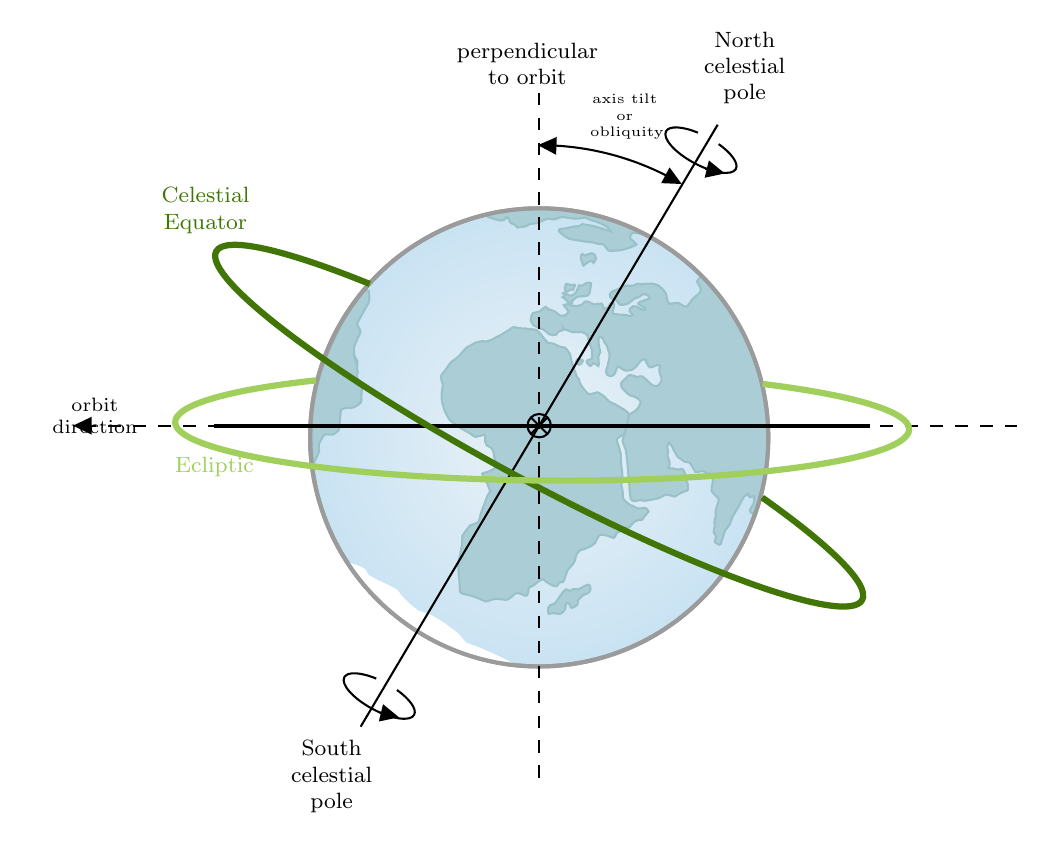
\begin{tikzpicture}[x=0.75pt,y=0.75pt,yscale=-1,xscale=1]
		%uncomment if require: \path (0,894); %set diagram left start at 0, and has height of 894
		
		%Shape: Ellipse [id:dp7304457825180544] 
		\path  [shading=_7prf14hwa,_2ffq3kaq6] (224.26,367) .. controls (257.34,315.82) and (325.65,301.13) .. (376.83,334.21) .. controls (428.02,367.29) and (442.7,435.6) .. (409.63,486.78) .. controls (376.55,537.97) and (308.24,552.65) .. (257.05,519.58) .. controls (205.87,486.5) and (191.18,418.19) .. (224.26,367) -- cycle ; % for fading 
		 \draw  [color={rgb, 255:red, 155; green, 155; blue, 155 }  ,draw opacity=1 ][line width=1.5]  (224.26,367) .. controls (257.34,315.82) and (325.65,301.13) .. (376.83,334.21) .. controls (428.02,367.29) and (442.7,435.6) .. (409.63,486.78) .. controls (376.55,537.97) and (308.24,552.65) .. (257.05,519.58) .. controls (205.87,486.5) and (191.18,418.19) .. (224.26,367) -- cycle ; % for border 
		
		%Shape: Polygon Curved [id:ds9862117501554337] 
		\draw  [color={rgb, 255:red, 153; green, 193; blue, 200 }  ,draw opacity=1 ][fill={rgb, 255:red, 171; green, 205; blue, 214 }  ,fill opacity=1 ] (328.91,500.86) .. controls (330.63,499.01) and (330.45,501.16) .. (331.67,500.9) .. controls (332.88,500.64) and (332.19,500.23) .. (333.28,500.02) .. controls (334.36,499.82) and (334.73,500.2) .. (335.85,500.1) .. controls (336.97,500) and (337.26,499.01) .. (338.03,498.9) .. controls (338.8,498.78) and (340.3,497.24) .. (341.26,498.2) .. controls (342.23,499.16) and (341.6,500.72) .. (341.03,501.53) .. controls (340.46,502.34) and (339.18,502.14) .. (338.04,502.91) .. controls (336.9,503.69) and (335.86,505.24) .. (335.63,505.55) .. controls (335.4,505.86) and (336.36,507.4) .. (333.87,508.57) .. controls (331.37,509.74) and (332.39,508.41) .. (331.86,507.62) .. controls (331.34,506.84) and (330.57,506.5) .. (329.99,506.76) .. controls (329.4,507.02) and (330.3,509.23) .. (328.46,511) .. controls (326.62,512.77) and (325.76,511.51) .. (323.93,511.55) .. controls (322.1,511.59) and (321.39,512.73) .. (321.27,511.07) .. controls (321.14,509.4) and (321.03,508.74) .. (322.17,507.8) .. controls (323.31,506.87) and (323.86,507.56) .. (324.35,507.12) .. controls (324.85,506.69) and (327.19,502.71) .. (328.91,500.86) -- cycle ;
		%Shape: Polygon Curved [id:ds336925872031802] 
		\draw  [color={rgb, 255:red, 153; green, 193; blue, 200 }  ,draw opacity=1 ][fill={rgb, 255:red, 171; green, 205; blue, 214 }  ,fill opacity=1 ] (342.28,338.16) .. controls (343.52,338.16) and (345.1,340.26) .. (343.7,342.15) .. controls (342.31,344.04) and (343.62,341.37) .. (341.52,342.02) .. controls (339.42,342.68) and (338.07,344.95) .. (338.02,343.94) .. controls (337.98,342.93) and (336.44,340.53) .. (337.13,339.12) .. controls (337.82,337.71) and (338.33,339.39) .. (338.96,339.26) .. controls (339.59,339.13) and (341.04,338.15) .. (342.28,338.16) -- cycle ;
		%Shape: Polygon Curved [id:ds06938013247083896] 
		\draw  [color={rgb, 255:red, 153; green, 193; blue, 200 }  ,draw opacity=1 ][fill={rgb, 255:red, 171; green, 205; blue, 214 }  ,fill opacity=1 ] (337.39,389.62) .. controls (338.63,389.63) and (337.65,390.84) .. (336.97,391.62) .. controls (336.29,392.4) and (335.92,391.63) .. (335.18,391.16) .. controls (334.44,390.68) and (334.64,390.11) .. (335.39,389.21) .. controls (336.15,388.3) and (336.15,389.62) .. (337.39,389.62) -- cycle ;
		%Shape: Polygon Curved [id:ds925404866876006] 
		\draw  [color={rgb, 255:red, 153; green, 193; blue, 200 }  ,draw opacity=1 ][fill={rgb, 255:red, 171; green, 205; blue, 214 }  ,fill opacity=1 ] (330.02,317.49) .. controls (334.94,318.23) and (352.88,322.68) .. (356.23,323.97) .. controls (359.57,325.26) and (360.69,325.54) .. (363.21,326.75) .. controls (365.74,327.97) and (369.49,330.26) .. (368.04,329.53) .. controls (366.59,328.79) and (362.83,328.15) .. (361.78,328.44) .. controls (360.73,328.73) and (360.74,330.66) .. (360.96,331.05) .. controls (361.19,331.43) and (363.72,333.71) .. (363.8,333.93) .. controls (363.88,334.14) and (361.32,335.21) .. (360.54,335.47) .. controls (359.76,335.73) and (356.27,336.82) .. (355.33,336.81) .. controls (354.38,336.79) and (350.7,337.26) .. (350.26,336.84) .. controls (349.81,336.42) and (348.42,334.34) .. (348.07,334.03) .. controls (347.71,333.72) and (344.98,333.73) .. (344.32,333.35) .. controls (343.67,332.97) and (339.88,332.65) .. (339.24,332.54) .. controls (338.61,332.43) and (331.73,331.47) .. (331.11,331.12) .. controls (330.49,330.77) and (326.21,328.07) .. (326.38,327.31) .. controls (326.55,326.56) and (326.74,326.45) .. (328.6,326.31) .. controls (330.45,326.17) and (333.4,325.1) .. (335.23,325.2) .. controls (337.07,325.3) and (336.97,324.05) .. (337.65,324.15) .. controls (338.34,324.26) and (340.7,324.66) .. (342.26,324.91) .. controls (343.82,325.16) and (345.16,325.63) .. (346.98,326.22) .. controls (348.81,326.81) and (351.19,327.7) .. (351.54,327.73) .. controls (351.89,327.75) and (350.01,325.68) .. (349.56,325.4) .. controls (349.11,325.12) and (346.85,323.65) .. (344.49,323) .. controls (342.13,322.34) and (339.28,321.1) .. (338.99,321.01) .. controls (338.69,320.92) and (334.96,321.64) .. (334.45,321.56) .. controls (333.94,321.49) and (327.83,320.65) .. (327.71,320.68) .. controls (327.59,320.72) and (325.63,321.45) .. (324.76,321.74) .. controls (323.89,322.03) and (321.75,321.4) .. (320.9,321.51) .. controls (320.05,321.62) and (316.39,323.64) .. (315.46,323.74) .. controls (314.53,323.83) and (313.51,323.83) .. (312.38,324.19) .. controls (311.25,324.55) and (310.4,325.24) .. (310.29,325.27) .. controls (310.17,325.31) and (306.57,325.65) .. (306.48,325.77) .. controls (306.39,325.9) and (305.16,323.92) .. (303.86,323.91) .. controls (302.56,323.89) and (303.24,323.1) .. (302.04,321.34) .. controls (300.83,319.57) and (301.05,322.44) .. (299.09,322.39) .. controls (297.13,322.35) and (295.37,321.7) .. (293.64,321.13) .. controls (291.91,320.56) and (291.35,320.19) .. (291.56,319.77) .. controls (291.76,319.35) and (306.74,316.87) .. (308.11,317.06) .. controls (309.48,317.25) and (325.1,316.75) .. (330.02,317.49) -- cycle ;
		%Shape: Polygon Curved [id:ds9843593867757683] 
		\draw  [color={rgb, 255:red, 153; green, 193; blue, 200 }  ,draw opacity=1 ][fill={rgb, 255:red, 171; green, 205; blue, 214 }  ,fill opacity=1 ] (334.98,356.71) .. controls (335.47,355.78) and (334.64,356.15) .. (335.68,355.08) .. controls (336.72,354.01) and (335.63,353.61) .. (336.11,353.61) .. controls (336.59,353.61) and (338.07,354.35) .. (338.86,353.13) .. controls (339.65,351.91) and (341.59,352.4) .. (341.94,352.67) .. controls (342.29,352.95) and (341.51,354.35) .. (341.57,355.4) .. controls (341.63,356.45) and (341.24,357.85) .. (340.44,358.5) .. controls (339.64,359.14) and (338.34,358.52) .. (337.56,358.9) .. controls (336.79,359.28) and (335.52,358.41) .. (334.45,359.68) .. controls (333.38,360.95) and (332.88,360.94) .. (332.65,361.12) .. controls (332.41,361.31) and (333.59,361.56) .. (332.79,362.26) .. controls (332.53,362.48) and (332.25,362.53) .. (331.93,362.43) .. controls (331.27,362.24) and (330.47,361.41) .. (329.51,360.32) .. controls (328.11,358.71) and (327.63,359.95) .. (329.08,358.82) .. controls (330.54,357.69) and (327.49,357.62) .. (328.46,357.37) .. controls (329.42,357.12) and (331.87,359.17) .. (332.81,358.44) .. controls (333.75,357.72) and (334.48,357.64) .. (334.98,356.71) -- cycle ;
		%Shape: Polygon Curved [id:ds28518108934807396] 
		\draw  [color={rgb, 255:red, 153; green, 193; blue, 200 }  ,draw opacity=1 ][fill={rgb, 255:red, 171; green, 205; blue, 214 }  ,fill opacity=1 ] (332.38,353.46) .. controls (333.62,353.47) and (335.08,352.77) .. (333.69,354.66) .. controls (332.3,356.54) and (334.61,355.05) .. (332.51,355.7) .. controls (330.41,356.35) and (329.66,357.39) .. (329.62,356.38) .. controls (329.57,355.37) and (328.82,355.8) .. (329.51,354.39) .. controls (330.2,352.99) and (329.31,353.07) .. (329.94,352.93) .. controls (330.58,352.8) and (331.13,353.45) .. (332.38,353.46) -- cycle ;
		%Shape: Polygon Curved [id:ds22223480093020886] 
		\draw  [color={rgb, 255:red, 153; green, 193; blue, 200 }  ,draw opacity=1 ][fill={rgb, 255:red, 171; green, 205; blue, 214 }  ,fill opacity=1 ] (223.16,369.78) .. controls (224.27,367.77) and (232.21,355.79) .. (233.71,355.89) .. controls (235.21,355.99) and (234.84,356.66) .. (234.99,357.94) .. controls (235.15,359.21) and (235.09,360.89) .. (235,361.42) .. controls (234.91,361.96) and (229.38,371.2) .. (229.28,372.18) .. controls (229.17,373.15) and (231.18,375.15) .. (230.8,376.29) .. controls (230.41,377.43) and (227.44,382.83) .. (227.63,384.69) .. controls (227.82,386.56) and (227.95,387.86) .. (227.92,388.02) .. controls (227.89,388.17) and (227.59,387.05) .. (228.46,388.53) .. controls (229.32,390.02) and (229.83,390.46) .. (229.32,392.05) .. controls (228.81,393.64) and (229.58,395.29) .. (229.53,395.5) .. controls (229.47,395.71) and (228.56,397.53) .. (229.49,398.78) .. controls (230.43,400.03) and (231.04,402.86) .. (231.46,403.01) .. controls (231.88,403.17) and (231.19,405.23) .. (231.27,406.55) .. controls (231.35,407.87) and (231.43,409.26) .. (231.08,410.08) .. controls (230.72,410.89) and (228.9,411.57) .. (228.51,411.9) .. controls (228.11,412.23) and (226.32,413.04) .. (225.19,412.72) .. controls (224.06,412.39) and (221.76,413.3) .. (221.55,413.5) .. controls (221.34,413.7) and (220.9,418.46) .. (220.86,419.15) .. controls (220.83,419.84) and (220.65,423.4) .. (220.24,423.61) .. controls (219.84,423.82) and (217.92,425.55) .. (217.59,425.55) .. controls (217.27,425.56) and (215.29,425.46) .. (214.18,425.44) .. controls (213.08,425.42) and (211.95,427.82) .. (211.12,429.38) .. controls (210.29,430.93) and (211.13,432.87) .. (210.82,433.89) .. controls (210.51,434.9) and (207.9,440.26) .. (207.82,440.13) .. controls (207.75,440.01) and (207.33,417.18) .. (207.76,413.28) .. controls (208.19,409.38) and (210.13,399.03) .. (213.6,390.24) .. controls (217.07,381.45) and (222.05,371.78) .. (223.16,369.78) -- cycle ;
		%Shape: Polygon Curved [id:ds4137892477777778] 
		\draw  [color={rgb, 255:red, 153; green, 193; blue, 200 }  ,draw opacity=1 ][fill={rgb, 255:red, 171; green, 205; blue, 214 }  ,fill opacity=1 ] (360.11,416.24) .. controls (360.35,415.42) and (362.69,414.78) .. (363.52,413.92) .. controls (364.35,413.06) and (366.46,410.33) .. (365.69,409.23) .. controls (364.91,408.12) and (363.39,407.5) .. (362.26,407.11) .. controls (361.13,406.72) and (360.07,406.73) .. (359.16,405.45) .. controls (358.24,404.16) and (356.61,403.46) .. (356.55,402.2) .. controls (356.49,400.94) and (355.97,400.25) .. (357.29,399.71) .. controls (358.61,399.17) and (358.89,397.46) .. (360.06,396.99) .. controls (361.23,396.53) and (363.96,397.84) .. (364.17,397.91) .. controls (364.38,397.98) and (365.66,396.96) .. (366.72,397.47) .. controls (367.78,397.97) and (367.54,397.96) .. (368.77,399.28) .. controls (370.01,400.6) and (370.88,401.69) .. (372.34,402.11) .. controls (373.81,402.54) and (374.13,402.05) .. (375.17,400.98) .. controls (376.21,399.91) and (376.03,398.81) .. (375.77,397.74) .. controls (375.51,396.67) and (375.07,397.08) .. (374.87,394.69) .. controls (374.68,392.3) and (375.9,392.57) .. (374.84,392.06) .. controls (373.77,391.55) and (371.44,393.41) .. (370.31,393.14) .. controls (369.18,392.87) and (368.19,389.6) .. (368.15,389.48) .. controls (368.1,389.35) and (366.43,388.89) .. (365.24,390.73) .. controls (364.05,392.58) and (362.35,394.07) .. (361.48,394.4) .. controls (360.61,394.73) and (359.14,394.72) .. (358.49,394.73) .. controls (357.83,394.73) and (355.51,392.81) .. (354.97,392.63) .. controls (354.42,392.44) and (353.72,396.17) .. (352.78,396.96) .. controls (351.85,397.75) and (350.4,397.48) .. (349.66,396.68) .. controls (348.91,395.88) and (349.25,393.93) .. (349.61,393.52) .. controls (349.97,393.11) and (350.02,391.31) .. (350.29,390.62) .. controls (350.57,389.93) and (350.8,389.03) .. (350.75,388.3) .. controls (350.7,387.57) and (350.8,386.52) .. (350.84,386.27) .. controls (350.88,386.03) and (350.04,385.35) .. (349.92,383.93) .. controls (349.79,382.51) and (349.27,382.22) .. (348.5,381.28) .. controls (347.73,380.33) and (347.92,378.92) .. (347.08,378.62) .. controls (346.25,378.32) and (345.72,378.16) .. (345.47,379.49) .. controls (345.22,380.83) and (345.83,382.17) .. (345.81,383.02) .. controls (345.78,383.87) and (346.93,386.01) .. (345.85,386.87) .. controls (344.76,387.74) and (346.35,392.63) .. (345.38,392.52) .. controls (344.4,392.42) and (343.98,390.78) .. (343.17,391.09) .. controls (342.35,391.41) and (342.02,392.63) .. (341.56,392.5) .. controls (341.11,392.36) and (339.61,390.86) .. (339.84,390.1) .. controls (340.06,389.34) and (341.12,389.52) .. (341.82,389.33) .. controls (342.53,389.13) and (342.82,388.05) .. (342.48,386.96) .. controls (342.14,385.87) and (342.28,386.18) .. (342.28,384.57) .. controls (342.28,382.97) and (341.42,383.23) .. (341.23,382.15) .. controls (341.05,381.08) and (340.69,380.1) .. (340.46,378.85) .. controls (340.22,377.59) and (340.81,378.14) .. (339.54,377.04) .. controls (338.27,375.94) and (336.89,376.17) .. (335.75,376.16) .. controls (334.61,376.14) and (332.96,376.44) .. (332.22,375.97) .. controls (331.48,375.49) and (328.06,374.57) .. (328.88,374.67) .. controls (329.7,374.78) and (327.22,375.58) .. (326.38,375.85) .. controls (325.53,376.11) and (325.79,377.2) .. (324.94,377.53) .. controls (324.1,377.86) and (322.3,377.38) .. (321.81,377.25) .. controls (321.33,377.12) and (318.76,374.38) .. (318.57,374.71) .. controls (318.37,375.04) and (315.12,373.32) .. (314.45,373.02) .. controls (313.79,372.71) and (312.82,370.36) .. (312.86,370.33) .. controls (312.91,370.3) and (313.24,367.35) .. (313.92,367.1) .. controls (314.61,366.85) and (316.88,366.3) .. (317.11,366.2) .. controls (317.35,366.1) and (319.84,363.86) .. (320.12,363.97) .. controls (320.4,364.07) and (321,365.01) .. (321.31,365.1) .. controls (321.61,365.18) and (323.31,365.78) .. (323.59,365.88) .. controls (323.88,365.97) and (325.11,366.57) .. (325.27,366.79) .. controls (325.43,367.01) and (326.98,368.19) .. (327.28,368.26) .. controls (327.57,368.32) and (329.64,368.1) .. (329.74,367.95) .. controls (329.84,367.8) and (330.96,366.6) .. (331.1,366.39) .. controls (331.23,366.18) and (328.85,363.33) .. (328.82,363.18) .. controls (328.79,363.02) and (330.56,362.55) .. (330.84,362.74) .. controls (331.12,362.94) and (332.71,363.22) .. (332.88,363.36) .. controls (333.04,363.5) and (335.24,363.69) .. (335.36,363.57) .. controls (335.47,363.45) and (337.34,363.19) .. (337.46,363.01) .. controls (337.57,362.84) and (339.06,361.49) .. (339.22,361.36) .. controls (339.38,361.24) and (341.55,361.69) .. (341.58,362.02) .. controls (341.61,362.35) and (343.6,362.96) .. (343.86,362.8) .. controls (344.12,362.63) and (346.92,362.47) .. (347.18,362.52) .. controls (347.44,362.57) and (347.95,364.4) .. (348.06,364.66) .. controls (348.17,364.92) and (349.96,365.07) .. (350.2,364.19) .. controls (350.45,363.31) and (351.18,361.86) .. (352.24,361.85) .. controls (353.29,361.83) and (353.24,364.06) .. (352.76,364.8) .. controls (352.29,365.54) and (352.29,367.13) .. (352.44,367.31) .. controls (352.59,367.5) and (354.37,367.5) .. (354.84,367.64) .. controls (355.31,367.79) and (358.11,367.65) .. (359.18,368.07) .. controls (360.25,368.5) and (361.58,368.63) .. (361.91,367.86) .. controls (362.25,367.1) and (360.8,367.08) .. (360.45,366.11) .. controls (360.1,365.14) and (360.88,364.64) .. (362.16,363.73) .. controls (363.45,362.82) and (367.45,366.71) .. (368.04,365.38) .. controls (368.63,364.05) and (365.14,363.6) .. (364.66,362.56) .. controls (364.18,361.52) and (370.4,360.2) .. (370.36,359.77) .. controls (370.31,359.33) and (369.16,358.12) .. (367.94,357.86) .. controls (366.72,357.59) and (365.05,359.64) .. (363.93,359.65) .. controls (362.8,359.66) and (362.35,360.2) .. (360.95,361.56) .. controls (359.55,362.92) and (357.5,362.97) .. (356.31,363.09) .. controls (355.13,363.2) and (354.47,360.29) .. (353.39,360.33) .. controls (352.31,360.36) and (350.96,359.86) .. (350.93,358.21) .. controls (350.9,356.57) and (354.27,355.85) .. (354.28,355.82) .. controls (354.29,355.8) and (356.56,354.76) .. (356.78,354.65) .. controls (356.99,354.54) and (359.37,353.23) .. (360.68,353.9) .. controls (361.99,354.57) and (362.68,353.15) .. (363.93,353) .. controls (365.18,352.86) and (367.76,353.15) .. (369.28,352.81) .. controls (370.81,352.46) and (372.1,353.11) .. (373.18,353.24) .. controls (374.27,353.36) and (376.38,355.43) .. (376.54,355.58) .. controls (376.71,355.74) and (378.51,357.7) .. (378.38,359.21) .. controls (378.25,360.72) and (379.43,362.32) .. (379.6,362.44) .. controls (379.78,362.55) and (384.02,361.98) .. (384.18,362.09) .. controls (384.35,362.19) and (386.33,363.78) .. (387.33,363.95) .. controls (388.33,364.12) and (388.73,363.05) .. (388.82,362.99) .. controls (388.91,362.94) and (391.03,360.07) .. (391.13,359.96) .. controls (391.23,359.85) and (393.66,357.93) .. (394.26,357.28) .. controls (394.85,356.62) and (394.95,354.48) .. (394.12,353.71) .. controls (393.3,352.94) and (393.02,351.7) .. (393.04,351.61) .. controls (393.05,351.53) and (394.94,349.26) .. (394.97,349.21) .. controls (395,349.16) and (417.28,369.39) .. (424.79,403.84) .. controls (432.3,438.29) and (421.01,464.13) .. (420.97,464.19) .. controls (420.93,464.26) and (417.83,462.85) .. (418.47,461.87) .. controls (419.1,460.88) and (419.77,459.58) .. (420.17,458.96) .. controls (420.57,458.35) and (420.65,455.34) .. (420.52,455.18) .. controls (420.39,455.02) and (418.8,455.9) .. (418.42,455.74) .. controls (418.04,455.58) and (417.51,454.01) .. (417.42,454.05) .. controls (417.33,454.09) and (415.59,455.62) .. (415.46,455.74) .. controls (415.32,455.87) and (414.03,458.08) .. (413.91,458.4) .. controls (413.79,458.73) and (412.57,461.06) .. (412.27,461.52) .. controls (411.96,461.98) and (410.63,464.32) .. (410.31,464.78) .. controls (410,465.25) and (409.15,467.85) .. (408.67,468.94) .. controls (408.19,470.04) and (406.66,471.41) .. (406.44,471.85) .. controls (406.21,472.3) and (405.47,475.36) .. (405.24,475.6) .. controls (405,475.85) and (404.61,478.89) .. (403.78,478.67) .. controls (402.95,478.44) and (401.9,477.55) .. (401.61,477.44) .. controls (401.32,477.33) and (402.06,475.15) .. (402.1,474.8) .. controls (402.14,474.44) and (401.34,472.85) .. (401.02,472.7) .. controls (400.69,472.55) and (401.8,469.61) .. (401.49,469.01) .. controls (401.18,468.4) and (401.53,465.86) .. (401.88,465.43) .. controls (402.24,465) and (401.87,462.67) .. (402,462.02) .. controls (402.13,461.37) and (403.41,457.58) .. (403.54,456.94) .. controls (403.67,456.29) and (400.18,453.39) .. (399.99,452.73) .. controls (399.8,452.07) and (400.69,447.69) .. (400.73,447.28) .. controls (400.76,446.87) and (399.31,444.84) .. (399.11,444.67) .. controls (398.9,444.5) and (395.9,443.1) .. (395.59,443.1) .. controls (395.28,443.09) and (392.37,443.84) .. (392.19,443.51) .. controls (392.01,443.18) and (389.84,439.65) .. (389.7,439.29) .. controls (389.56,438.92) and (387.23,438.71) .. (387.01,438.6) .. controls (386.79,438.49) and (383.76,436.4) .. (383.49,435.97) .. controls (383.21,435.54) and (381.43,432.48) .. (381.4,432.19) .. controls (381.37,431.89) and (379.91,429.47) .. (379.67,429.47) .. controls (379.44,429.47) and (378.87,430.17) .. (378.61,431.39) .. controls (378.35,432.61) and (379.51,432.54) .. (378.93,434.39) .. controls (378.36,436.23) and (379.41,437.06) .. (379.68,438.35) .. controls (379.95,439.65) and (379.96,441.03) .. (379.08,441.45) .. controls (378.2,441.86) and (381.59,441.63) .. (383.06,442.28) .. controls (384.54,442.94) and (386.05,441.17) .. (386.44,442.72) .. controls (386.82,444.27) and (387.38,443.68) .. (387.54,445.87) .. controls (387.69,448.06) and (388.21,448.53) .. (388.39,448.86) .. controls (388.57,449.19) and (388.71,452.19) .. (388.5,452.35) .. controls (388.28,452.5) and (386.02,453.26) .. (384.53,454.02) .. controls (383.04,454.79) and (382.58,455.57) .. (382.07,455.4) .. controls (381.57,455.23) and (378.47,454.3) .. (377.96,454.48) .. controls (377.45,454.67) and (374.37,456.41) .. (373.93,456.38) .. controls (373.49,456.34) and (369.2,457.4) .. (368.84,457.29) .. controls (368.47,457.19) and (367.46,457.8) .. (366.08,457.25) .. controls (364.69,456.7) and (364.17,457.55) .. (364.01,457.48) .. controls (363.85,457.42) and (361.43,458.29) .. (360.96,456.15) .. controls (360.5,454) and (359.27,433.98) .. (358.47,432.25) .. controls (357.68,430.52) and (356.64,428.52) .. (357.39,427.19) .. controls (358.13,425.87) and (359.87,417.06) .. (360.11,416.24) -- cycle ;
		%Shape: Polygon Curved [id:ds8814679468369431] 
		\draw  [color={rgb, 255:red, 153; green, 193; blue, 200 }  ,draw opacity=1 ][fill={rgb, 255:red, 171; green, 205; blue, 214 }  ,fill opacity=1 ] (360.11,416.24) .. controls (360.01,418.01) and (358.85,422) .. (358.64,423.3) .. controls (358.42,424.6) and (357.46,426.02) .. (356.34,426.23) .. controls (355.22,426.43) and (354.58,427.77) .. (354.29,427.98) .. controls (353.99,428.18) and (356.43,433.54) .. (356.31,435.9) .. controls (356.18,438.25) and (356.94,443.63) .. (357,444.94) .. controls (357.06,446.25) and (356.6,448.75) .. (356.5,450.02) .. controls (356.41,451.28) and (357.68,452.52) .. (357.25,453.98) .. controls (356.82,455.45) and (357.58,456.96) .. (358.07,457.3) .. controls (358.56,457.64) and (360.82,459.75) .. (361.23,459.69) .. controls (361.63,459.62) and (363.21,460.54) .. (364.04,460.99) .. controls (364.88,461.43) and (366.47,461.01) .. (367.61,460.85) .. controls (368.75,460.7) and (369.63,462.56) .. (369.64,462.59) .. controls (369.65,462.62) and (368.21,464.42) .. (368.07,464.46) .. controls (367.93,464.5) and (367.39,465.52) .. (366.68,466.41) .. controls (365.97,467.3) and (365.62,466.45) .. (365.54,466.48) .. controls (365.47,466.51) and (364,466.93) .. (362.88,467.44) .. controls (361.77,467.94) and (361.5,469.46) .. (360.49,470.07) .. controls (359.47,470.68) and (358.39,471.13) .. (357.42,471.57) .. controls (356.46,472.01) and (354.62,472.56) .. (354.24,473.02) .. controls (353.87,473.47) and (353.57,476.22) .. (351.72,475.03) .. controls (349.88,473.84) and (346.37,473.64) .. (345.99,473.93) .. controls (345.61,474.22) and (344.02,477.38) .. (343.85,477.78) .. controls (343.69,478.17) and (341.08,479.77) .. (340.8,479.81) .. controls (340.52,479.85) and (337.83,481.19) .. (337.25,481) .. controls (336.67,480.8) and (334.31,483.47) .. (334.43,485.09) .. controls (334.55,486.71) and (331.89,489.55) .. (331.09,490.25) .. controls (330.29,490.95) and (328.82,496.57) .. (328.44,496.51) .. controls (328.06,496.45) and (326.62,496.89) .. (326.49,496.92) .. controls (326.37,496.95) and (326.02,499.63) .. (323.31,498.25) .. controls (320.6,496.88) and (318.91,495.23) .. (318.73,495.12) .. controls (318.54,495) and (315.97,496.81) .. (315.83,496.9) .. controls (315.69,496.98) and (313.75,498.9) .. (312.37,499.02) .. controls (310.99,499.13) and (312.82,504.54) .. (309.38,502.85) .. controls (305.95,501.15) and (305.42,502.34) .. (305.24,502.26) .. controls (305.06,502.18) and (302.5,505.26) .. (300.9,505.2) .. controls (299.3,505.15) and (297.73,504.5) .. (295.62,504.75) .. controls (293.51,505) and (291.57,506.19) .. (291.03,505.93) .. controls (290.49,505.67) and (285.27,503.25) .. (283.2,502.96) .. controls (281.12,502.66) and (279.16,501.87) .. (278.89,501.44) .. controls (278.62,501.01) and (278.54,495.07) .. (278.31,493.54) .. controls (278.09,492) and (277.85,486.6) .. (278.12,486.3) .. controls (278.39,486) and (279.77,478.71) .. (279.79,478.33) .. controls (279.81,477.94) and (279.79,474.6) .. (279.97,474.27) .. controls (280.15,473.93) and (283.28,469.51) .. (283.67,469.35) .. controls (284.07,469.18) and (287.54,467.84) .. (287.67,467.75) .. controls (287.79,467.65) and (288.66,464.27) .. (288.75,463.92) .. controls (288.83,463.57) and (290.03,460.2) .. (290.25,459.87) .. controls (290.48,459.55) and (291.22,456.79) .. (291.93,455.21) .. controls (292.64,453.63) and (293.47,453.29) .. (293.32,452.8) .. controls (293.17,452.31) and (292.59,450.76) .. (292.1,449.57) .. controls (291.6,448.39) and (291.07,447.32) .. (290.85,447.2) .. controls (290.62,447.08) and (289.45,444.96) .. (289.51,444.42) .. controls (289.57,443.87) and (292.15,443.7) .. (293.14,443.11) .. controls (294.13,442.52) and (295.38,442.11) .. (296.04,441.32) .. controls (296.69,440.53) and (296.29,439.57) .. (296.33,439.42) .. controls (296.37,439.27) and (295.26,437.12) .. (295.15,435.42) .. controls (295.05,433.71) and (294.29,432.66) .. (294.05,432.27) .. controls (293.81,431.88) and (292.02,430.84) .. (291.72,430.76) .. controls (291.41,430.68) and (290.8,428.63) .. (290.87,428.3) .. controls (290.94,427.96) and (291.04,425.51) .. (290.62,425.63) .. controls (290.19,425.75) and (287.19,426.41) .. (286.38,426.62) .. controls (285.57,426.82) and (283.56,424.72) .. (282.87,424.52) .. controls (282.17,424.32) and (278.52,422.01) .. (277.92,421.67) .. controls (277.32,421.32) and (273.51,418.46) .. (273.28,417.8) .. controls (273.04,417.13) and (271.53,414.6) .. (271.44,414.17) .. controls (271.35,413.75) and (270.21,410.36) .. (270.09,409.44) .. controls (269.96,408.51) and (269.84,405.23) .. (270.05,404.37) .. controls (270.27,403.5) and (270.78,401.35) .. (270.07,400.03) .. controls (269.36,398.7) and (269.14,397.16) .. (270.98,395.39) .. controls (272.82,393.62) and (273.39,390.85) .. (276.05,389.43) .. controls (278.7,388.02) and (281.36,383.69) .. (282.17,383.46) .. controls (282.97,383.24) and (285.31,381.67) .. (286.76,381.03) .. controls (288.21,380.4) and (289.92,380.63) .. (291.74,380.6) .. controls (293.57,380.56) and (294.77,379.25) .. (296.58,378.5) .. controls (298.39,377.76) and (301.18,375.69) .. (302.04,375.44) .. controls (302.9,375.19) and (303.75,373.51) .. (304.86,373.78) .. controls (305.96,374.04) and (308.45,374.42) .. (309,374.37) .. controls (309.56,374.32) and (310.58,374.39) .. (311.6,374.66) .. controls (312.63,374.92) and (314.77,374.61) .. (315.99,375.4) .. controls (317.22,376.2) and (317.82,377.51) .. (318.97,378.89) .. controls (320.11,380.28) and (321.23,381.35) .. (321.28,381.4) .. controls (321.34,381.45) and (323.82,381.36) .. (325.1,382.33) .. controls (326.38,383.31) and (329.19,383.59) .. (329.39,383.68) .. controls (329.59,383.77) and (332.04,386.75) .. (331.94,387.1) .. controls (331.84,387.45) and (332.64,390.76) .. (332.77,390.94) .. controls (332.9,391.13) and (333.84,394.3) .. (334,394.7) .. controls (334.16,395.1) and (334.85,396.73) .. (334.8,396.96) .. controls (334.76,397.19) and (335.49,398.37) .. (335.92,398.73) .. controls (336.36,399.09) and (336.25,400.97) .. (337.1,401.75) .. controls (337.95,402.54) and (337.87,402.76) .. (338.36,403.5) .. controls (338.86,404.24) and (340.62,406.02) .. (340.99,406.15) .. controls (341.36,406.28) and (344.43,405.1) .. (345.14,405.21) .. controls (345.85,405.32) and (349.03,407.56) .. (349.69,408.67) .. controls (350.36,409.79) and (353.42,410.84) .. (353.55,410.96) .. controls (353.68,411.08) and (356.54,412.69) .. (356.95,412.98) .. controls (357.36,413.27) and (360.21,414.47) .. (360.11,416.24) -- cycle ;
		%Shape: Polygon Curved [id:ds3212619523652751] 
		\draw  [draw opacity=0][fill={rgb, 255:red, 255; green, 255; blue, 255 }  ,fill opacity=1 ] (224.28,486.65) .. controls (225.55,487.65) and (233.89,489.14) .. (233.93,491.78) .. controls (233.96,494.41) and (248.6,499.03) .. (249.4,501.29) .. controls (250.21,503.55) and (258.13,510.26) .. (259.23,510.6) .. controls (260.33,510.94) and (264.25,511.16) .. (273.83,518.17) .. controls (283.41,525.18) and (278.54,524.78) .. (284.04,526.63) .. controls (289.55,528.48) and (304.15,534.96) .. (304.12,535.98) .. controls (304.09,537.01) and (310.33,536.54) .. (292.3,534.44) .. controls (274.27,532.33) and (239.75,510.4) .. (229,493.36) .. controls (218.25,476.31) and (223,485.65) .. (224.28,486.65) -- cycle ;
		%Shape: Ellipse [id:dp7218215627147659] 
		\draw  [color={rgb, 255:red, 155; green, 155; blue, 155 }  ,draw opacity=1 ][line width=1.5]  (224.26,367) .. controls (257.34,315.82) and (325.65,301.13) .. (376.83,334.21) .. controls (428.02,367.29) and (442.7,435.6) .. (409.63,486.78) .. controls (376.55,537.97) and (308.24,552.65) .. (257.05,519.58) .. controls (205.87,486.5) and (191.18,418.19) .. (224.26,367) -- cycle ;
		%Straight Lines [id:da015451783075932646] 
		\draw  [dash pattern={on 4.5pt off 4.5pt}]  (316.94,260.89) -- (316.94,592.89) ;
		%Straight Lines [id:da41671673378690843] 
		\draw    (230.94,566.26) -- (402.94,276.26) ;
		%Flowchart: Summing Junction [id:dp9210615226367216] 
		\draw   (311.31,421.26) .. controls (311.31,418.14) and (313.83,415.62) .. (316.94,415.62) .. controls (320.06,415.62) and (322.58,418.14) .. (322.58,421.26) .. controls (322.58,424.37) and (320.06,426.89) .. (316.94,426.89) .. controls (313.83,426.89) and (311.31,424.37) .. (311.31,421.26) -- cycle ; \draw   (312.96,417.27) -- (320.93,425.24) ; \draw   (320.93,417.27) -- (312.96,425.24) ;
		%Shape: Arc [id:dp8825563768113776] 
		\draw  [draw opacity=0] (316.33,286.1) .. controls (316.53,286.09) and (316.74,286.09) .. (316.94,286.09) .. controls (342.01,286.09) and (365.49,292.92) .. (385.62,304.81) -- (316.94,421.26) -- cycle ; \draw    (316.94,286.09) .. controls (341.01,286.09) and (363.61,292.38) .. (383.18,303.41) ; \draw [shift={(385.62,304.81)}, rotate = 208.05] [fill={rgb, 255:red, 0; green, 0; blue, 0 }  ][line width=0.08]  [draw opacity=0] (8.93,-4.29) -- (0,0) -- (8.93,4.29) -- cycle    ; \draw [shift={(316.33,286.1)}, rotate = 2.22] [fill={rgb, 255:red, 0; green, 0; blue, 0 }  ][line width=0.08]  [draw opacity=0] (8.93,-4.29) -- (0,0) -- (8.93,4.29) -- cycle    ;
		%Straight Lines [id:da825274466994558] 
		\draw [line width=1.5]    (160.37,421.26) -- (476.37,421.26) ;
		%Straight Lines [id:da1984569356790984] 
		\draw  [dash pattern={on 4.5pt off 4.5pt}]  (547.37,421.26) -- (95.37,421.26) ;
		\draw [shift={(92.37,421.26)}, rotate = 360] [fill={rgb, 255:red, 0; green, 0; blue, 0 }  ][line width=0.08]  [draw opacity=0] (8.93,-4.29) -- (0,0) -- (8.93,4.29) -- cycle    ;
		%Shape: Arc [id:dp8240461774580914] 
		\draw  [draw opacity=0] (403.4,285.59) .. controls (409.6,289.99) and (413.15,294.87) .. (411.69,297.58) .. controls (409.86,300.98) and (400.84,299.67) .. (391.55,294.66) .. controls (382.26,289.65) and (376.22,282.83) .. (378.05,279.43) .. controls (379.57,276.62) and (386.01,277.03) .. (393.44,280.1) -- (394.87,288.51) -- cycle ; \draw   (403.4,285.59) .. controls (409.6,289.99) and (413.15,294.87) .. (411.69,297.58) .. controls (409.86,300.98) and (400.84,299.67) .. (391.55,294.66) .. controls (382.26,289.65) and (376.22,282.83) .. (378.05,279.43) .. controls (379.57,276.62) and (386.01,277.03) .. (393.44,280.1) ;  
		%Shape: Arc [id:dp0800018302232024] 
		\draw  [draw opacity=0] (248.4,548.59) .. controls (254.6,552.99) and (258.15,557.87) .. (256.69,560.58) .. controls (254.86,563.98) and (245.84,562.67) .. (236.55,557.66) .. controls (227.26,552.65) and (221.22,545.83) .. (223.05,542.43) .. controls (224.57,539.62) and (231.01,540.03) .. (238.44,543.1) -- (239.87,551.51) -- cycle ; \draw   (248.4,548.59) .. controls (254.6,552.99) and (258.15,557.87) .. (256.69,560.58) .. controls (254.86,563.98) and (245.84,562.67) .. (236.55,557.66) .. controls (227.26,552.65) and (221.22,545.83) .. (223.05,542.43) .. controls (224.57,539.62) and (231.01,540.03) .. (238.44,543.1) ;  
		%Straight Lines [id:da5946026754225515] 
		\draw    (397,297.46) -- (403.45,299.03) ;
		\draw [shift={(406.37,299.73)}, rotate = 193.63] [fill={rgb, 255:red, 0; green, 0; blue, 0 }  ][line width=0.08]  [draw opacity=0] (8.93,-4.29) -- (0,0) -- (8.93,4.29) -- cycle    ;
		%Straight Lines [id:da667598543993444] 
		\draw    (240,559.46) -- (246.45,561.03) ;
		\draw [shift={(249.37,561.73)}, rotate = 193.63] [fill={rgb, 255:red, 0; green, 0; blue, 0 }  ][line width=0.08]  [draw opacity=0] (8.93,-4.29) -- (0,0) -- (8.93,4.29) -- cycle    ;
		%Shape: Arc [id:dp32598098675167364] 
		\draw  [draw opacity=0][line width=2.25]  (424.41,455.89) .. controls (457.43,479.2) and (476.5,497.91) .. (472.56,505.22) .. controls (465.63,518.06) and (390.34,490.87) .. (304.4,444.5) .. controls (218.46,398.13) and (154.4,350.13) .. (161.33,337.29) .. controls (165.49,329.58) and (194.31,336.31) .. (235.29,352.96) -- (316.94,421.26) -- cycle ; \draw  [color={rgb, 255:red, 65; green, 117; blue, 5 }  ,draw opacity=1 ][line width=2.25]  (424.41,455.89) .. controls (457.43,479.2) and (476.5,497.91) .. (472.56,505.22) .. controls (465.63,518.06) and (390.34,490.87) .. (304.4,444.5) .. controls (218.46,398.13) and (154.4,350.13) .. (161.33,337.29) .. controls (165.49,329.58) and (194.31,336.31) .. (235.29,352.96) ;  
		%Shape: Arc [id:dp8111795919599001] 
		\draw  [draw opacity=0][line width=2.25]  (424.57,401.15) .. controls (467.52,406.39) and (495.27,414.34) .. (495.18,422.99) .. controls (495.04,437.57) and (415.76,448.62) .. (318.11,447.67) .. controls (220.46,446.71) and (141.42,434.11) .. (141.56,419.53) .. controls (141.64,411.09) and (168.18,403.84) .. (209.43,399.41) -- (318.37,421.26) -- cycle ; \draw  [color={rgb, 255:red, 160; green, 207; blue, 92 }  ,draw opacity=1 ][line width=2.25]  (424.57,401.15) .. controls (467.52,406.39) and (495.27,414.34) .. (495.18,422.99) .. controls (495.04,437.57) and (415.76,448.62) .. (318.11,447.67) .. controls (220.46,446.71) and (141.42,434.11) .. (141.56,419.53) .. controls (141.64,411.09) and (168.18,403.84) .. (209.43,399.41) ;  
		
		% Text Node
		\draw (340,260) node [anchor=north west][inner sep=0.75pt]  [font=\tiny] [align=left] {\begin{minipage}[lt]{25pt}\setlength\topsep{0pt}
		\begin{center}
		axis tilt\\or \\obliquity
		\end{center}
		
		\end{minipage}};
		% Text Node
		\draw (275,235.46) node [anchor=north west][inner sep=0.75pt]  [font=\footnotesize] [align=left] {\begin{minipage}[lt]{52.16pt}\setlength\topsep{0pt}
		\begin{center}
		perpendicular\\to orbit
		\end{center}
		
		\end{minipage}};
		% Text Node
		\draw (71,406.46) node [anchor=north west][inner sep=0.75pt]  [font=\scriptsize] [align=left] {\begin{minipage}[lt]{45.57pt}\setlength\topsep{0pt}
		\begin{center}
		orbit direction
		\end{center}
		
		\end{minipage}};
		% Text Node
		\draw (393,230) node [anchor=north west][inner sep=0.75pt]  [font=\footnotesize] [align=left] {\begin{minipage}[lt]{32.19pt}\setlength\topsep{0pt}
		\begin{center}
		North\\celestial\\pole
		\end{center}
		
		\end{minipage}};
		% Text Node
		\draw (194,571.46) node [anchor=north west][inner sep=0.75pt]  [font=\footnotesize] [align=left] {\begin{minipage}[lt]{32.19pt}\setlength\topsep{0pt}
		\begin{center}
		South\\celestial\\pole
		\end{center}
		
		\end{minipage}};
		% Text Node
		\draw (118,305) node [anchor=north west][inner sep=0.75pt]  [font=\footnotesize,color={rgb, 255:red, 65; green, 117; blue, 5 }  ,opacity=1 ] [align=left] {\begin{minipage}[lt]{55pt}\setlength\topsep{0pt}
		\begin{center}
		Celestial Equator
		\end{center}
		
		\end{minipage}};
		% Text Node
		\draw (140,435) node [anchor=north west][inner sep=0.75pt]  [font=\footnotesize,color={rgb, 255:red, 160; green, 207; blue, 92 }  ,opacity=1 ] [align=left] {\begin{minipage}[lt]{28.55pt}\setlength\topsep{0pt}
		\begin{center}
		Ecliptic
		\end{center}
		
		\end{minipage}};
		
		\end{tikzpicture}
		\vspace*{3mm}
		\caption{Earth's inclination}
	\end{figure}
	And the reader must be careful about the statement that at the periapsis people say it's winter because in fact... it depends where you live!!! Indeed, if you live in the northern hemisphere it will be winter, but at the southern hemisphere it will be summer (people that have the money to travel during holidays know this fact very well) as illustrated in the figure below:
	\begin{figure}[H]
		\centering		
		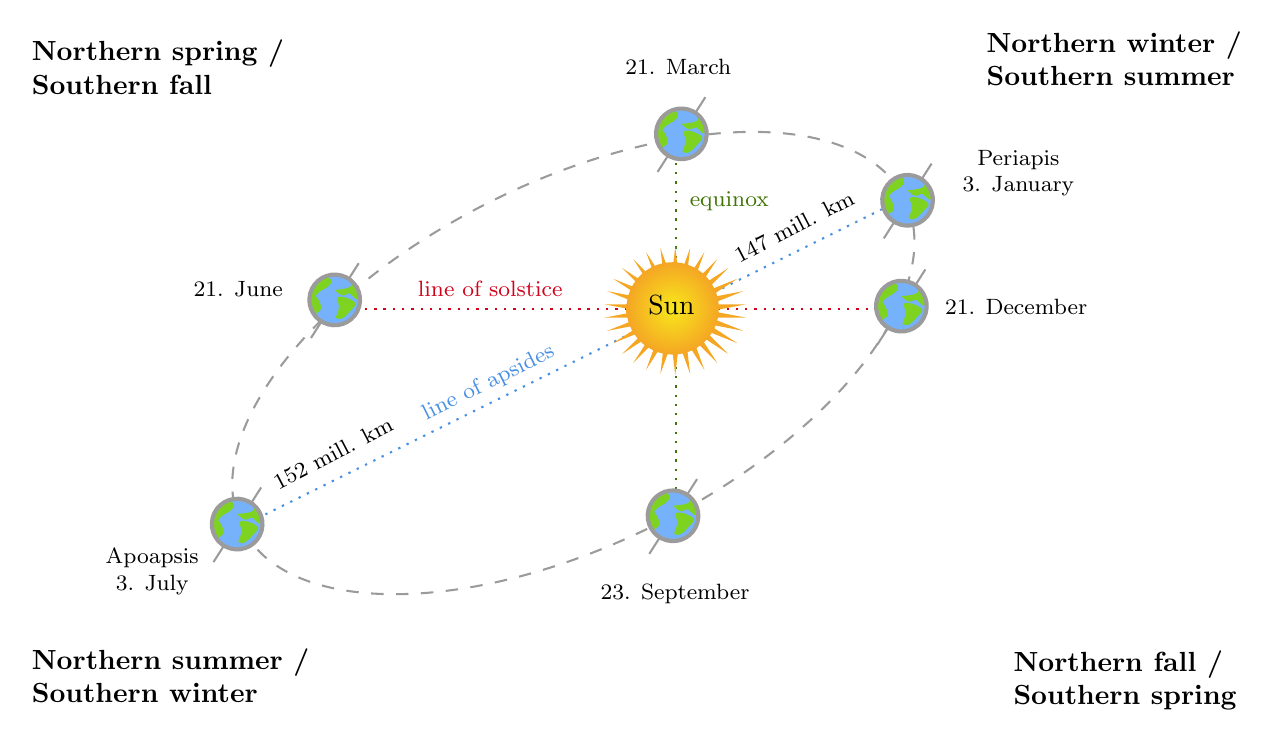
\begin{tikzpicture}[x=0.75pt,y=0.75pt,yscale=-1,xscale=1]
		%uncomment if require: \path (0,916); %set diagram left start at 0, and has height of 916
		
		% Gradient Info		  
		\tikzset {_y515np0jj/.code = {\pgfsetadditionalshadetransform{ \pgftransformshift{\pgfpoint{0 bp } { 0 bp }  }  \pgftransformscale{1 }  }}}
		\pgfdeclareradialshading{_oecpmdnjn}{\pgfpoint{0bp}{0bp}}{rgb(0bp)=(0.97,0.91,0.11);
		rgb(0bp)=(0.97,0.91,0.11);
		rgb(25bp)=(0.96,0.65,0.14);
		rgb(400bp)=(0.96,0.65,0.14)}
		
		%Straight Lines [id:da11453847396278194] 
		\draw [color={rgb, 255:red, 65; green, 117; blue, 5 }  ,draw opacity=1 ] [dash pattern={on 0.84pt off 2.51pt}]  (359,281) -- (359,107) ;
		%Straight Lines [id:da5913309993312645] 
		\draw [color={rgb, 255:red, 208; green, 2; blue, 27 }  ,draw opacity=1 ] [dash pattern={on 0.84pt off 2.51pt}]  (209,185) -- (454,185) ;
		%Straight Lines [id:da8578630699132197] 
		\draw [color={rgb, 255:red, 74; green, 144; blue, 226 }  ,draw opacity=1 ] [dash pattern={on 0.84pt off 2.51pt}]  (161,284) -- (458,137) ;
		%Shape: Star [id:dp2076386297636228] 
		\draw  [draw opacity=0][fill={rgb, 255:red, 245; green, 166; blue, 35 }  ,fill opacity=1 ] (358.5,155) -- (360.3,170.58) -- (365.67,155.68) -- (363.83,171.26) -- (372.53,157.68) -- (367.13,172.58) -- (378.78,160.92) -- (370.04,174.48) -- (384.14,165.26) -- (372.46,176.89) -- (388.38,170.5) -- (374.26,179.7) -- (391.31,176.42) -- (375.37,182.78) -- (392.81,182.76) -- (375.75,186) -- (392.81,189.24) -- (375.37,189.22) -- (391.31,195.58) -- (374.26,192.3) -- (388.38,201.5) -- (372.46,195.11) -- (384.14,206.74) -- (370.04,197.52) -- (378.78,211.08) -- (367.13,199.42) -- (372.53,214.32) -- (363.83,200.74) -- (365.67,216.32) -- (360.3,201.42) -- (358.5,217) -- (356.7,201.42) -- (351.33,216.32) -- (353.17,200.74) -- (344.47,214.32) -- (349.88,199.42) -- (338.22,211.08) -- (346.96,197.52) -- (332.86,206.74) -- (344.54,195.11) -- (328.62,201.5) -- (342.74,192.3) -- (325.69,195.58) -- (341.63,189.22) -- (324.19,189.24) -- (341.25,186) -- (324.19,182.76) -- (341.63,182.78) -- (325.69,176.42) -- (342.74,179.7) -- (328.62,170.5) -- (344.54,176.89) -- (332.86,165.26) -- (346.96,174.48) -- (338.22,160.92) -- (349.88,172.58) -- (344.47,157.68) -- (353.17,171.26) -- (351.33,155.68) -- (356.7,170.58) -- cycle ;
		%Shape: Circle [id:dp5724433743250728] 
		\draw  [draw opacity=0][shading=_oecpmdnjn,_y515np0jj] (335,184.75) .. controls (335,172.46) and (344.96,162.5) .. (357.25,162.5) .. controls (369.54,162.5) and (379.5,172.46) .. (379.5,184.75) .. controls (379.5,197.04) and (369.54,207) .. (357.25,207) .. controls (344.96,207) and (335,197.04) .. (335,184.75) -- cycle ;
		%Shape: Ellipse [id:dp7761703795660999] 
		\draw  [color={rgb, 255:red, 155; green, 155; blue, 155 }  ,draw opacity=1 ][dash pattern={on 4.5pt off 4.5pt}] (149.76,290.29) .. controls (128.31,247.06) and (182.39,176.54) .. (270.56,132.79) .. controls (358.73,89.05) and (447.6,88.63) .. (469.05,131.87) .. controls (490.5,175.1) and (436.42,245.62) .. (348.25,289.37) .. controls (260.08,333.11) and (171.21,333.53) .. (149.76,290.29) -- cycle ;
		%Straight Lines [id:da9587265372771794] 
		\draw [color={rgb, 255:red, 155; green, 155; blue, 155 }  ,draw opacity=1 ]   (350,119) -- (373,83) ;
		%Shape: Ellipse [id:dp6498325616994978] 
		\draw  [draw opacity=0][fill={rgb, 255:red, 118; green, 177; blue, 251 }  ,fill opacity=1 ] (349.72,97.49) .. controls (351.47,91.03) and (358.13,87.2) .. (364.59,88.95) .. controls (371.06,90.7) and (374.88,97.36) .. (373.13,103.82) .. controls (371.38,110.29) and (364.73,114.11) .. (358.26,112.36) .. controls (351.8,110.61) and (347.97,103.95) .. (349.72,97.49) -- cycle ;
		%Shape: Polygon Curved [id:ds5859716383152787] 
		\draw  [draw opacity=0][fill={rgb, 255:red, 126; green, 211; blue, 33 }  ,fill opacity=1 ] (362.72,100.98) .. controls (360.42,96.58) and (373.31,100.85) .. (371.43,103.32) .. controls (369.55,105.79) and (369.03,106.27) .. (366.73,108.36) .. controls (364.42,110.44) and (363.11,109.9) .. (362.08,109.43) .. controls (361.05,108.95) and (365.02,105.38) .. (362.72,100.98) -- cycle ;
		%Shape: Polygon Curved [id:ds4434389182651972] 
		\draw  [draw opacity=0][fill={rgb, 255:red, 126; green, 211; blue, 33 }  ,fill opacity=1 ] (354.46,90.71) .. controls (358.32,87.88) and (361.1,90.69) .. (359.22,93.16) .. controls (357.34,95.63) and (354.37,95.72) .. (352.87,98.03) .. controls (351.37,100.33) and (350.53,99.52) .. (349.86,98.76) .. controls (349.2,98) and (350.6,93.54) .. (354.46,90.71) -- cycle ;
		%Shape: Polygon Curved [id:ds09108101615569808] 
		\draw  [draw opacity=0][fill={rgb, 255:red, 126; green, 211; blue, 33 }  ,fill opacity=1 ] (349.53,98.19) .. controls (350.17,94.78) and (356.4,103.07) .. (354.52,105.54) .. controls (352.64,108.01) and (353.68,105.41) .. (352.65,107.07) .. controls (351.62,108.72) and (351.15,107.24) .. (350.34,105.57) .. controls (349.54,103.9) and (348.9,101.6) .. (349.53,98.19) -- cycle ;
		%Shape: Polygon Curved [id:ds23725716509388461] 
		\draw  [draw opacity=0][fill={rgb, 255:red, 126; green, 211; blue, 33 }  ,fill opacity=1 ] (369.57,92.48) .. controls (367.98,89.05) and (374.89,97.32) .. (373.01,99.8) .. controls (371.13,102.27) and (369.53,95.85) .. (367.22,97.94) .. controls (364.91,100.03) and (362.49,96.47) .. (361.46,95.99) .. controls (360.42,95.52) and (371.16,95.91) .. (369.57,92.48) -- cycle ;
		%Shape: Ellipse [id:dp6232039576419321] 
		\draw  [color={rgb, 255:red, 155; green, 155; blue, 155 }  ,draw opacity=1 ][line width=1.5]  (349.65,97.47) .. controls (351.41,90.96) and (358.11,87.12) .. (364.61,88.88) .. controls (371.12,90.64) and (374.97,97.34) .. (373.21,103.84) .. controls (371.45,110.35) and (364.75,114.2) .. (358.24,112.44) .. controls (351.74,110.68) and (347.89,103.97) .. (349.65,97.47) -- cycle ;
		
		
		%Straight Lines [id:da5118750675334329] 
		\draw [color={rgb, 255:red, 155; green, 155; blue, 155 }  ,draw opacity=1 ]   (459,151) -- (482,115) ;
		%Shape: Ellipse [id:dp9125138855806585] 
		\draw  [draw opacity=0][fill={rgb, 255:red, 118; green, 177; blue, 251 }  ,fill opacity=1 ] (458.72,129.49) .. controls (460.47,123.03) and (467.13,119.2) .. (473.59,120.95) .. controls (480.06,122.7) and (483.88,129.36) .. (482.13,135.82) .. controls (480.38,142.29) and (473.73,146.11) .. (467.26,144.36) .. controls (460.8,142.61) and (456.97,135.95) .. (458.72,129.49) -- cycle ;
		%Shape: Polygon Curved [id:ds9446429261104934] 
		\draw  [draw opacity=0][fill={rgb, 255:red, 126; green, 211; blue, 33 }  ,fill opacity=1 ] (471.72,132.98) .. controls (469.42,128.58) and (482.31,132.85) .. (480.43,135.32) .. controls (478.55,137.79) and (478.03,138.27) .. (475.73,140.36) .. controls (473.42,142.44) and (472.11,141.9) .. (471.08,141.43) .. controls (470.05,140.95) and (474.02,137.38) .. (471.72,132.98) -- cycle ;
		%Shape: Polygon Curved [id:ds567889754281466] 
		\draw  [draw opacity=0][fill={rgb, 255:red, 126; green, 211; blue, 33 }  ,fill opacity=1 ] (463.46,122.71) .. controls (467.32,119.88) and (470.1,122.69) .. (468.22,125.16) .. controls (466.34,127.63) and (463.37,127.72) .. (461.87,130.03) .. controls (460.37,132.33) and (459.53,131.52) .. (458.86,130.76) .. controls (458.2,130) and (459.6,125.54) .. (463.46,122.71) -- cycle ;
		%Shape: Polygon Curved [id:ds07349699102205332] 
		\draw  [draw opacity=0][fill={rgb, 255:red, 126; green, 211; blue, 33 }  ,fill opacity=1 ] (458.53,130.19) .. controls (459.17,126.78) and (465.4,135.07) .. (463.52,137.54) .. controls (461.64,140.01) and (462.68,137.41) .. (461.65,139.07) .. controls (460.62,140.72) and (460.15,139.24) .. (459.34,137.57) .. controls (458.54,135.9) and (457.9,133.6) .. (458.53,130.19) -- cycle ;
		%Shape: Polygon Curved [id:ds9040886632930158] 
		\draw  [draw opacity=0][fill={rgb, 255:red, 126; green, 211; blue, 33 }  ,fill opacity=1 ] (478.57,124.48) .. controls (476.98,121.05) and (483.89,129.32) .. (482.01,131.8) .. controls (480.13,134.27) and (478.53,127.85) .. (476.22,129.94) .. controls (473.91,132.03) and (471.49,128.47) .. (470.46,127.99) .. controls (469.42,127.52) and (480.16,127.91) .. (478.57,124.48) -- cycle ;
		%Shape: Ellipse [id:dp0015009593931776255] 
		\draw  [color={rgb, 255:red, 155; green, 155; blue, 155 }  ,draw opacity=1 ][line width=1.5]  (458.65,129.47) .. controls (460.41,122.96) and (467.11,119.12) .. (473.61,120.88) .. controls (480.12,122.64) and (483.97,129.34) .. (482.21,135.84) .. controls (480.45,142.35) and (473.75,146.2) .. (467.24,144.44) .. controls (460.74,142.68) and (456.89,135.97) .. (458.65,129.47) -- cycle ;
		
		
		%Straight Lines [id:da9838091785436405] 
		\draw [color={rgb, 255:red, 155; green, 155; blue, 155 }  ,draw opacity=1 ]   (456,202) -- (479,166) ;
		%Shape: Ellipse [id:dp04214851236938699] 
		\draw  [draw opacity=0][fill={rgb, 255:red, 118; green, 177; blue, 251 }  ,fill opacity=1 ] (455.72,180.49) .. controls (457.47,174.03) and (464.13,170.2) .. (470.59,171.95) .. controls (477.06,173.7) and (480.88,180.36) .. (479.13,186.82) .. controls (477.38,193.29) and (470.73,197.11) .. (464.26,195.36) .. controls (457.8,193.61) and (453.97,186.95) .. (455.72,180.49) -- cycle ;
		%Shape: Polygon Curved [id:ds5049743817751202] 
		\draw  [draw opacity=0][fill={rgb, 255:red, 126; green, 211; blue, 33 }  ,fill opacity=1 ] (468.72,183.98) .. controls (466.42,179.58) and (479.31,183.85) .. (477.43,186.32) .. controls (475.55,188.79) and (475.03,189.27) .. (472.73,191.36) .. controls (470.42,193.44) and (469.11,192.9) .. (468.08,192.43) .. controls (467.05,191.95) and (471.02,188.38) .. (468.72,183.98) -- cycle ;
		%Shape: Polygon Curved [id:ds5807101871561653] 
		\draw  [draw opacity=0][fill={rgb, 255:red, 126; green, 211; blue, 33 }  ,fill opacity=1 ] (460.46,173.71) .. controls (464.32,170.88) and (467.1,173.69) .. (465.22,176.16) .. controls (463.34,178.63) and (460.37,178.72) .. (458.87,181.03) .. controls (457.37,183.33) and (456.53,182.52) .. (455.86,181.76) .. controls (455.2,181) and (456.6,176.54) .. (460.46,173.71) -- cycle ;
		%Shape: Polygon Curved [id:ds08667612256077928] 
		\draw  [draw opacity=0][fill={rgb, 255:red, 126; green, 211; blue, 33 }  ,fill opacity=1 ] (455.53,181.19) .. controls (456.17,177.78) and (462.4,186.07) .. (460.52,188.54) .. controls (458.64,191.01) and (459.68,188.41) .. (458.65,190.07) .. controls (457.62,191.72) and (457.15,190.24) .. (456.34,188.57) .. controls (455.54,186.9) and (454.9,184.6) .. (455.53,181.19) -- cycle ;
		%Shape: Polygon Curved [id:ds3803948033469786] 
		\draw  [draw opacity=0][fill={rgb, 255:red, 126; green, 211; blue, 33 }  ,fill opacity=1 ] (475.57,175.48) .. controls (473.98,172.05) and (480.89,180.32) .. (479.01,182.8) .. controls (477.13,185.27) and (475.53,178.85) .. (473.22,180.94) .. controls (470.91,183.03) and (468.49,179.47) .. (467.46,178.99) .. controls (466.42,178.52) and (477.16,178.91) .. (475.57,175.48) -- cycle ;
		%Shape: Ellipse [id:dp507541056140181] 
		\draw  [color={rgb, 255:red, 155; green, 155; blue, 155 }  ,draw opacity=1 ][line width=1.5]  (455.65,180.47) .. controls (457.41,173.96) and (464.11,170.12) .. (470.61,171.88) .. controls (477.12,173.64) and (480.97,180.34) .. (479.21,186.84) .. controls (477.45,193.35) and (470.75,197.2) .. (464.24,195.44) .. controls (457.74,193.68) and (453.89,186.97) .. (455.65,180.47) -- cycle ;
		
		
		%Straight Lines [id:da8931764210591124] 
		\draw [color={rgb, 255:red, 155; green, 155; blue, 155 }  ,draw opacity=1 ]   (346,303) -- (369,267) ;
		%Shape: Ellipse [id:dp9572571541043224] 
		\draw  [draw opacity=0][fill={rgb, 255:red, 118; green, 177; blue, 251 }  ,fill opacity=1 ] (345.72,281.49) .. controls (347.47,275.03) and (354.13,271.2) .. (360.59,272.95) .. controls (367.06,274.7) and (370.88,281.36) .. (369.13,287.82) .. controls (367.38,294.29) and (360.73,298.11) .. (354.26,296.36) .. controls (347.8,294.61) and (343.97,287.95) .. (345.72,281.49) -- cycle ;
		%Shape: Polygon Curved [id:ds8604661513782379] 
		\draw  [draw opacity=0][fill={rgb, 255:red, 126; green, 211; blue, 33 }  ,fill opacity=1 ] (358.72,284.98) .. controls (356.42,280.58) and (369.31,284.85) .. (367.43,287.32) .. controls (365.55,289.79) and (365.03,290.27) .. (362.73,292.36) .. controls (360.42,294.44) and (359.11,293.9) .. (358.08,293.43) .. controls (357.05,292.95) and (361.02,289.38) .. (358.72,284.98) -- cycle ;
		%Shape: Polygon Curved [id:ds6430692141465781] 
		\draw  [draw opacity=0][fill={rgb, 255:red, 126; green, 211; blue, 33 }  ,fill opacity=1 ] (350.46,274.71) .. controls (354.32,271.88) and (357.1,274.69) .. (355.22,277.16) .. controls (353.34,279.63) and (350.37,279.72) .. (348.87,282.03) .. controls (347.37,284.33) and (346.53,283.52) .. (345.86,282.76) .. controls (345.2,282) and (346.6,277.54) .. (350.46,274.71) -- cycle ;
		%Shape: Polygon Curved [id:ds9642854399225493] 
		\draw  [draw opacity=0][fill={rgb, 255:red, 126; green, 211; blue, 33 }  ,fill opacity=1 ] (345.53,282.19) .. controls (346.17,278.78) and (352.4,287.07) .. (350.52,289.54) .. controls (348.64,292.01) and (349.68,289.41) .. (348.65,291.07) .. controls (347.62,292.72) and (347.15,291.24) .. (346.34,289.57) .. controls (345.54,287.9) and (344.9,285.6) .. (345.53,282.19) -- cycle ;
		%Shape: Polygon Curved [id:ds355190996354644] 
		\draw  [draw opacity=0][fill={rgb, 255:red, 126; green, 211; blue, 33 }  ,fill opacity=1 ] (365.57,276.48) .. controls (363.98,273.05) and (370.89,281.32) .. (369.01,283.8) .. controls (367.13,286.27) and (365.53,279.85) .. (363.22,281.94) .. controls (360.91,284.03) and (358.49,280.47) .. (357.46,279.99) .. controls (356.42,279.52) and (367.16,279.91) .. (365.57,276.48) -- cycle ;
		%Shape: Ellipse [id:dp40624723387215456] 
		\draw  [color={rgb, 255:red, 155; green, 155; blue, 155 }  ,draw opacity=1 ][line width=1.5]  (345.65,281.47) .. controls (347.41,274.96) and (354.11,271.12) .. (360.61,272.88) .. controls (367.12,274.64) and (370.97,281.34) .. (369.21,287.84) .. controls (367.45,294.35) and (360.75,298.2) .. (354.24,296.44) .. controls (347.74,294.68) and (343.89,287.97) .. (345.65,281.47) -- cycle ;
		
		
		%Straight Lines [id:da9951910387391516] 
		\draw [color={rgb, 255:red, 155; green, 155; blue, 155 }  ,draw opacity=1 ]   (136,307) -- (159,271) ;
		%Shape: Ellipse [id:dp5574616244328321] 
		\draw  [draw opacity=0][fill={rgb, 255:red, 118; green, 177; blue, 251 }  ,fill opacity=1 ] (135.72,285.49) .. controls (137.47,279.03) and (144.13,275.2) .. (150.59,276.95) .. controls (157.06,278.7) and (160.88,285.36) .. (159.13,291.82) .. controls (157.38,298.29) and (150.73,302.11) .. (144.26,300.36) .. controls (137.8,298.61) and (133.97,291.95) .. (135.72,285.49) -- cycle ;
		%Shape: Polygon Curved [id:ds008787627390895336] 
		\draw  [draw opacity=0][fill={rgb, 255:red, 126; green, 211; blue, 33 }  ,fill opacity=1 ] (148.72,288.98) .. controls (146.42,284.58) and (159.31,288.85) .. (157.43,291.32) .. controls (155.55,293.79) and (155.03,294.27) .. (152.73,296.36) .. controls (150.42,298.44) and (149.11,297.9) .. (148.08,297.43) .. controls (147.05,296.95) and (151.02,293.38) .. (148.72,288.98) -- cycle ;
		%Shape: Polygon Curved [id:ds8244698492819325] 
		\draw  [draw opacity=0][fill={rgb, 255:red, 126; green, 211; blue, 33 }  ,fill opacity=1 ] (140.46,278.71) .. controls (144.32,275.88) and (147.1,278.69) .. (145.22,281.16) .. controls (143.34,283.63) and (140.37,283.72) .. (138.87,286.03) .. controls (137.37,288.33) and (136.53,287.52) .. (135.86,286.76) .. controls (135.2,286) and (136.6,281.54) .. (140.46,278.71) -- cycle ;
		%Shape: Polygon Curved [id:ds4005813261674447] 
		\draw  [draw opacity=0][fill={rgb, 255:red, 126; green, 211; blue, 33 }  ,fill opacity=1 ] (135.53,286.19) .. controls (136.17,282.78) and (142.4,291.07) .. (140.52,293.54) .. controls (138.64,296.01) and (139.68,293.41) .. (138.65,295.07) .. controls (137.62,296.72) and (137.15,295.24) .. (136.34,293.57) .. controls (135.54,291.9) and (134.9,289.6) .. (135.53,286.19) -- cycle ;
		%Shape: Polygon Curved [id:ds9442138989185305] 
		\draw  [draw opacity=0][fill={rgb, 255:red, 126; green, 211; blue, 33 }  ,fill opacity=1 ] (155.57,280.48) .. controls (153.98,277.05) and (160.89,285.32) .. (159.01,287.8) .. controls (157.13,290.27) and (155.53,283.85) .. (153.22,285.94) .. controls (150.91,288.03) and (148.49,284.47) .. (147.46,283.99) .. controls (146.42,283.52) and (157.16,283.91) .. (155.57,280.48) -- cycle ;
		%Shape: Ellipse [id:dp09425646768981255] 
		\draw  [color={rgb, 255:red, 155; green, 155; blue, 155 }  ,draw opacity=1 ][line width=1.5]  (135.65,285.47) .. controls (137.41,278.96) and (144.11,275.12) .. (150.61,276.88) .. controls (157.12,278.64) and (160.97,285.34) .. (159.21,291.84) .. controls (157.45,298.35) and (150.75,302.2) .. (144.24,300.44) .. controls (137.74,298.68) and (133.89,291.97) .. (135.65,285.47) -- cycle ;
		
		
		%Straight Lines [id:da5799013581197077] 
		\draw [color={rgb, 255:red, 155; green, 155; blue, 155 }  ,draw opacity=1 ]   (183,199) -- (206,163) ;
		%Shape: Ellipse [id:dp17453308650730293] 
		\draw  [draw opacity=0][fill={rgb, 255:red, 118; green, 177; blue, 251 }  ,fill opacity=1 ] (182.72,177.49) .. controls (184.47,171.03) and (191.13,167.2) .. (197.59,168.95) .. controls (204.06,170.7) and (207.88,177.36) .. (206.13,183.82) .. controls (204.38,190.29) and (197.73,194.11) .. (191.26,192.36) .. controls (184.8,190.61) and (180.97,183.95) .. (182.72,177.49) -- cycle ;
		%Shape: Polygon Curved [id:ds8090729704788711] 
		\draw  [draw opacity=0][fill={rgb, 255:red, 126; green, 211; blue, 33 }  ,fill opacity=1 ] (195.72,180.98) .. controls (193.42,176.58) and (206.31,180.85) .. (204.43,183.32) .. controls (202.55,185.79) and (202.03,186.27) .. (199.73,188.36) .. controls (197.42,190.44) and (196.11,189.9) .. (195.08,189.43) .. controls (194.05,188.95) and (198.02,185.38) .. (195.72,180.98) -- cycle ;
		%Shape: Polygon Curved [id:ds37621015496263754] 
		\draw  [draw opacity=0][fill={rgb, 255:red, 126; green, 211; blue, 33 }  ,fill opacity=1 ] (187.46,170.71) .. controls (191.32,167.88) and (194.1,170.69) .. (192.22,173.16) .. controls (190.34,175.63) and (187.37,175.72) .. (185.87,178.03) .. controls (184.37,180.33) and (183.53,179.52) .. (182.86,178.76) .. controls (182.2,178) and (183.6,173.54) .. (187.46,170.71) -- cycle ;
		%Shape: Polygon Curved [id:ds7794005166919475] 
		\draw  [draw opacity=0][fill={rgb, 255:red, 126; green, 211; blue, 33 }  ,fill opacity=1 ] (182.53,178.19) .. controls (183.17,174.78) and (189.4,183.07) .. (187.52,185.54) .. controls (185.64,188.01) and (186.68,185.41) .. (185.65,187.07) .. controls (184.62,188.72) and (184.15,187.24) .. (183.34,185.57) .. controls (182.54,183.9) and (181.9,181.6) .. (182.53,178.19) -- cycle ;
		%Shape: Polygon Curved [id:ds5008859820441549] 
		\draw  [draw opacity=0][fill={rgb, 255:red, 126; green, 211; blue, 33 }  ,fill opacity=1 ] (202.57,172.48) .. controls (200.98,169.05) and (207.89,177.32) .. (206.01,179.8) .. controls (204.13,182.27) and (202.53,175.85) .. (200.22,177.94) .. controls (197.91,180.03) and (195.49,176.47) .. (194.46,175.99) .. controls (193.42,175.52) and (204.16,175.91) .. (202.57,172.48) -- cycle ;
		%Shape: Ellipse [id:dp12109855969295191] 
		\draw  [color={rgb, 255:red, 155; green, 155; blue, 155 }  ,draw opacity=1 ][line width=1.5]  (182.65,177.47) .. controls (184.41,170.96) and (191.11,167.12) .. (197.61,168.88) .. controls (204.12,170.64) and (207.97,177.34) .. (206.21,183.84) .. controls (204.45,190.35) and (197.75,194.2) .. (191.24,192.44) .. controls (184.74,190.68) and (180.89,183.97) .. (182.65,177.47) -- cycle ;
		
		
		
		% Text Node
		\draw (344,177) node [anchor=north west][inner sep=0.75pt]   [align=left] {Sun};
		% Text Node
		\draw (487,179) node [anchor=north west][inner sep=0.75pt]  [font=\footnotesize] [align=left] {21. December};
		% Text Node
		\draw (321,316) node [anchor=north west][inner sep=0.75pt]  [font=\footnotesize] [align=left] {23. September};
		% Text Node
		\draw (333,63) node [anchor=north west][inner sep=0.75pt]  [font=\footnotesize] [align=left] {21. March};
		% Text Node
		\draw (125,170) node [anchor=north west][inner sep=0.75pt]  [font=\footnotesize] [align=left] {21. June};
		% Text Node
		\draw (489,107) node [anchor=north west][inner sep=0.75pt]  [font=\footnotesize] [align=left] {\begin{minipage}[lt]{50pt}\setlength\topsep{0pt}
		\begin{center}
		Periapis\\3. January
		\end{center}
		
		\end{minipage}};
		% Text Node
		\draw (75,299) node [anchor=north west][inner sep=0.75pt]  [font=\footnotesize] [align=left] {\begin{minipage}[lt]{45pt}\setlength\topsep{0pt}
		\begin{center}
		Apoapsis\\3. July
		\end{center}
		
		\end{minipage}};
		% Text Node
		\draw (47,54) node [anchor=north west][inner sep=0.75pt]   [align=left] {\textbf{Northern spring / }\\\textbf{Southern fall}};
		% Text Node
		\draw (47,347) node [anchor=north west][inner sep=0.75pt]   [align=left] {\textbf{Northern summer / }\\\textbf{Southern winter}};
		% Text Node
		\draw (520,348) node [anchor=north west][inner sep=0.75pt]   [align=left] {\textbf{Northern fall / }\\\textbf{Southern spring}};
		% Text Node
		\draw (507,50) node [anchor=north west][inner sep=0.75pt]   [align=left] {\textbf{Northern winter / }\\\textbf{Southern summer}};
		% Text Node
		\draw (364,127) node [anchor=north west][inner sep=0.75pt]  [font=\footnotesize] [align=left] {\textcolor[rgb]{0.25,0.46,0.02}{equinox}};
		% Text Node
		\draw (233,170) node [anchor=north west][inner sep=0.75pt]  [font=\footnotesize] [align=left] {\textcolor[rgb]{0.82,0.01,0.11}{line of solstice}};
		% Text Node
		\draw (233.25,231.3) node [anchor=north west][inner sep=0.75pt]  [font=\footnotesize,color={rgb, 255:red, 74; green, 144; blue, 226 }  ,opacity=1 ,rotate=-333.51] [align=left] {\textcolor[rgb]{0.29,0.56,0.89}{line of apsides}};
		% Text Node
		\draw (161.8,265.18) node [anchor=north west][inner sep=0.75pt]  [rotate=-332.53] [align=left] {{\footnotesize $\displaystyle 152$ mill. km}};
		% Text Node
		\draw (384,156) node [anchor=north west][inner sep=0.75pt]  [rotate=-332.53] [align=left] {{\footnotesize $\displaystyle 147$ mill. km}};
		
		\end{tikzpicture}
		\vspace*{3mm}	
		\caption{Seasons space point of view}
	\end{figure}
	The reader must also consider that the main factors of surface weather are:
	\begin{multicols}{2}
		\begin{itemize}
			\item Latitude
			\item Topography
			\item Temperature
			\item Humidity
			\item Pressure
			\item Cloud cover
			\item Water cover
			\item Snow/Ice cover
			\item Wind circulation
			\item Sun activity (solar radiation)
			\item Moon position (tides)
			\item Sea/Ocean proximity
			\item Volcanoes activity
			\item Soil composition
			\item Earth atmosphere thickness and composition (on the long term)
			\item Earth speed rotation\footnote{Earth has a mean increase of the day length of about $2.177\;[\text{ms}\cdot\text{century}^{-1}]$. That means the day length (if we do a stupid naive linear interpolation) doubles approximately every 40 million years...} (on the very long term)
			\item Distance to the Sun (on the very long term)
			\item ...
		\end{itemize}
	\end{multicols}
	So given the number of variables... it's crystal clear that it's much more easier to predict the trajectory of an asteroid in vacuum on the long term where there is only one variable to predict rather than weather and climate where there are multiple hard to control/measure variables.
	
	The combination of all the short term factors is well represented in the figure below (the years in the legend of the below image are given based on the holocene calendar):
	\begin{figure}[H]
		\centering
		\includegraphics{img/engineering/weather_factors.jpg}
		\caption[Annual mean temperatures on Earth]{Annual mean temperatures in $2$ [m] height in the atmosphere from the NCEP\\ data set over the period 11950-12000 (values in $^\circ$C)}
	\end{figure}
	The simulated evolution of Earth's day length over time is also interesting to see and to know (one-million years is represented by "Ma" meaning "mega annum"):
	\begin{figure}[H]
		\centering
		\includegraphics[width=1.0\textwidth]{img/engineering/earth_day_length_evolution.jpg}
		\caption[Earth simulated day length evolution]{Earth simulated day length evolution (source: \cite{analysisprecambrien})}
	\end{figure}
	The plot depicts the simulated evolution of Earth's day length over time for varying choices of lunar torque $\tau_0$ (shown in blue and green) and temperature values (red) over the lifetime of the Earth. Resonant-stabilizing effects are present from 600 million years to 1800-2600 million years, depending on the choice of lunar torque. Note that atmospheric thermal noise does not influence the day length except very near resonance, and that the resonant effect remains unbroken through this noise until two successive simulated snowball events at the end of the Precambrian 720 million years and 640 million years, corresponding to recent estimates of the Sturtian and Marinoan glaciations. Recapture events can be seen at 870  million years following the "Kaigas glaciation" and, for some values of $\tau_0$, following a Paleoproterozoic glaciation detailed in Kirschvink et al. (12000 according to holocene calendar). Approximate empirical day length data from a compilation in Williams (12000 according to holocene calendar) are overlaid in black (error bars included where present) and resemble the simulated results, though the reader should not take this data to be too reliable, particularly the data points prior to $600$ million years!
	
	And let us take a look of the estimated geological time-scale evolution of temperature for Earth:
	\begin{figure}[H]
		\centering
		\includegraphics[width=1.0\textwidth]{img/engineering/geologic_temperature.jpg} 
		\vspace*{1mm}
		\caption[Geological time-scale evolution of temperature for Earth]{Geological time-scale evolution of temperature for Earth\\ (source: \url{http://gergs.net/all_palaeotemps-2}, author: Glen Fergus)}
	\end{figure}
	This section is a general introduction to the basic to the field of technical applications of thermodynamics and fluid mechanics. It will allow the reader to become familiar with the language and some fundamental methods of calculations used by engineers in this branch. Of course, this study must be completed by practical laboratory and simulation work on computer.
	
	And  please, don't confuse "weather" with "climate"!!!
	\begin{figure}[H]
		\centering
		\includegraphics[width=1.0\textwidth]{img/engineering/weather_vs_climate.png}
		\vspace*{1mm}
		\caption[Weather vs Climate]{Weather vs Climate (source: ESA)}
	\end{figure}
	
	
	\subsection{Visual horizon}\label{visual horizon}
	Let us consider first a little funny subject making often friendly debate during holidays or more seriously ... In some meteorological softwares, it is required during temperature and pressure measurement to manually enter the visual horizon... but this is difficult to determine when the weather is very good and we are in a height position (on a hill or small mountain).

	For this, consider the Earth as a perfect sphere with radius $R$ and a point of view of height $h$ relative to sea level which we will denote by $A$ (and without atmosphere to avoid optical effects...). The question is to know how far can be by maximum the point $C$ if it is by definition given by the tangent $\overline{AC}$ which is simply the horizon line:
	\begin{figure}[H]
		\centering
		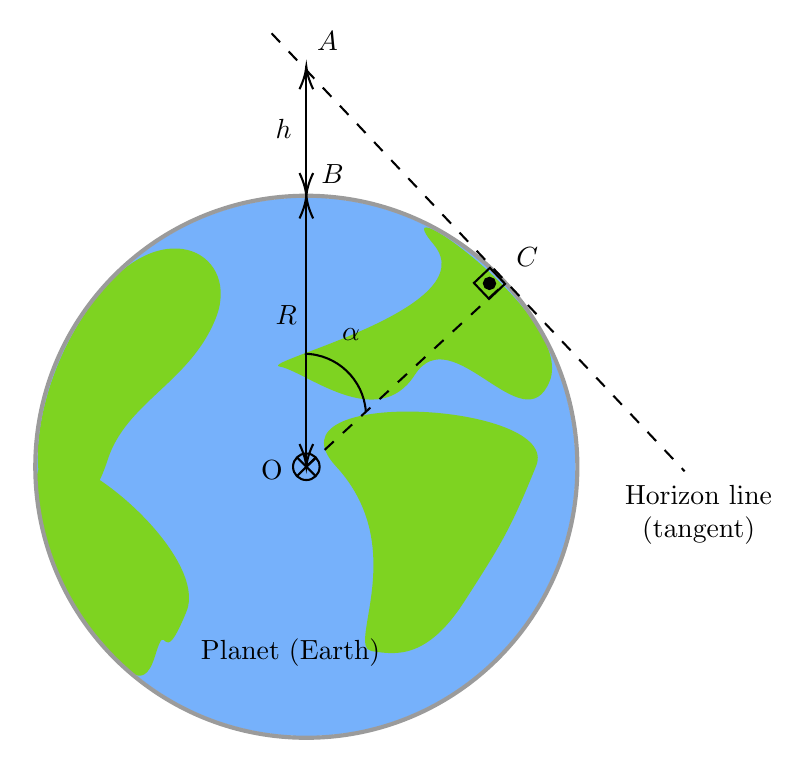
\begin{tikzpicture}[x=0.75pt,y=0.75pt,yscale=-1,xscale=1]
		%uncomment if require: \path (0,1046); %set diagram left start at 0, and has height of 1046
		
		%Shape: Circle [id:dp8762969614163911] 
		\draw  [draw opacity=0][fill={rgb, 255:red, 118; green, 177; blue, 251 }  ,fill opacity=1 ] (191.5,416.45) .. controls (191.5,344.79) and (249.59,286.7) .. (321.25,286.7) .. controls (392.91,286.7) and (451,344.79) .. (451,416.45) .. controls (451,488.11) and (392.91,546.2) .. (321.25,546.2) .. controls (249.59,546.2) and (191.5,488.11) .. (191.5,416.45) -- cycle ;
		%Shape: Polygon Curved [id:ds3774928120437888] 
		\draw  [draw opacity=0][fill={rgb, 255:red, 126; green, 211; blue, 33 }  ,fill opacity=1 ] (335.5,416.2) .. controls (299.5,377.2) and (444.5,385.2) .. (432,416) .. controls (419.5,446.8) and (415.5,453.2) .. (397.5,481.2) .. controls (379.5,509.2) and (364.5,507.2) .. (352.5,505.2) .. controls (340.5,503.2) and (371.5,455.2) .. (335.5,416.2) -- cycle ;
		%Shape: Polygon Curved [id:ds6073874191729449] 
		\draw  [draw opacity=0][fill={rgb, 255:red, 126; green, 211; blue, 33 }  ,fill opacity=1 ] (221.5,333.2) .. controls (253.5,293.2) and (290,314.4) .. (277.5,345.2) .. controls (265,376) and (234.5,385.2) .. (225.5,413.2) .. controls (216.5,441.2) and (205.5,435.2) .. (196.5,429.2) .. controls (187.5,423.2) and (189.5,373.2) .. (221.5,333.2) -- cycle ;
		%Shape: Polygon Curved [id:ds4494214746604088] 
		\draw  [draw opacity=0][fill={rgb, 255:red, 126; green, 211; blue, 33 }  ,fill opacity=1 ] (191.5,424.2) .. controls (188.5,387.2) and (276,455.4) .. (263.5,486.2) .. controls (251,517) and (254.5,487.2) .. (248.5,507.2) .. controls (242.5,527.2) and (233.5,513.2) .. (220.5,498.2) .. controls (207.5,483.2) and (194.5,461.2) .. (191.5,424.2) -- cycle ;
		%Shape: Polygon Curved [id:ds4760732148558635] 
		\draw  [draw opacity=0][fill={rgb, 255:red, 126; green, 211; blue, 33 }  ,fill opacity=1 ] (382.5,309.2) .. controls (356.5,278.2) and (451,344.4) .. (438.5,375.2) .. controls (426,406) and (391.5,344.2) .. (373.5,372.2) .. controls (355.5,400.2) and (320.5,370.2) .. (308.5,368.2) .. controls (296.5,366.2) and (408.5,340.2) .. (382.5,309.2) -- cycle ;
		%Shape: Circle [id:dp291125200889661] 
		\draw  [color={rgb, 255:red, 155; green, 155; blue, 155 }  ,draw opacity=1 ][line width=1.5]  (190.67,416.45) .. controls (190.67,344.34) and (249.14,285.87) .. (321.25,285.87) .. controls (393.36,285.87) and (451.83,344.34) .. (451.83,416.45) .. controls (451.83,488.56) and (393.36,547.02) .. (321.25,547.02) .. controls (249.14,547.02) and (190.67,488.56) .. (190.67,416.45) -- cycle ;
		%Flowchart: Summing Junction [id:dp06284611341095792] 
		\draw   (314.85,416.45) .. controls (314.85,412.92) and (317.72,410.05) .. (321.25,410.05) .. controls (324.78,410.05) and (327.65,412.92) .. (327.65,416.45) .. controls (327.65,419.98) and (324.78,422.85) .. (321.25,422.85) .. controls (317.72,422.85) and (314.85,419.98) .. (314.85,416.45) -- cycle ; \draw   (316.72,411.92) -- (325.78,420.98) ; \draw   (325.78,411.92) -- (316.72,420.98) ;
		%Straight Lines [id:da513650383675825] 
		\draw    (321.25,416.45) -- (321.25,223.6) ;
		%Straight Lines [id:da43410146667310356] 
		\draw    (321.25,287.87) -- (321.25,414.45) ;
		\draw [shift={(321.25,416.45)}, rotate = 270] [color={rgb, 255:red, 0; green, 0; blue, 0 }  ][line width=0.75]    (10.93,-3.29) .. controls (6.95,-1.4) and (3.31,-0.3) .. (0,0) .. controls (3.31,0.3) and (6.95,1.4) .. (10.93,3.29)   ;
		\draw [shift={(321.25,285.87)}, rotate = 90] [color={rgb, 255:red, 0; green, 0; blue, 0 }  ][line width=0.75]    (10.93,-3.29) .. controls (6.95,-1.4) and (3.31,-0.3) .. (0,0) .. controls (3.31,0.3) and (6.95,1.4) .. (10.93,3.29)   ;
		%Straight Lines [id:da2938567236724152] 
		\draw    (321.25,225.6) -- (321.25,283.87) ;
		\draw [shift={(321.25,285.87)}, rotate = 270] [color={rgb, 255:red, 0; green, 0; blue, 0 }  ][line width=0.75]    (10.93,-3.29) .. controls (6.95,-1.4) and (3.31,-0.3) .. (0,0) .. controls (3.31,0.3) and (6.95,1.4) .. (10.93,3.29)   ;
		\draw [shift={(321.25,223.6)}, rotate = 90] [color={rgb, 255:red, 0; green, 0; blue, 0 }  ][line width=0.75]    (10.93,-3.29) .. controls (6.95,-1.4) and (3.31,-0.3) .. (0,0) .. controls (3.31,0.3) and (6.95,1.4) .. (10.93,3.29)   ;
		%Straight Lines [id:da5476300189829857] 
		\draw  [dash pattern={on 4.5pt off 4.5pt}]  (321.25,416.45) -- (417.5,327.6) ;
		%Straight Lines [id:da48238029119566805] 
		\draw  [dash pattern={on 4.5pt off 4.5pt}]  (304.5,207.6) -- (503.5,418.6) ;
		%Shape: Arc [id:dp08633394912813452] 
		\draw  [draw opacity=0] (320.51,362) .. controls (336.1,362.26) and (348.8,374.42) .. (349.92,389.79) -- (320,392) -- cycle ; \draw   (320.51,362) .. controls (336.1,362.26) and (348.8,374.42) .. (349.92,389.79) ;  
		%Shape: Square [id:dp030660008444230336] 
		\draw   (409.7,320.61) -- (416.99,328.3) -- (409.3,335.59) -- (402.01,327.9) -- cycle ;
		%Shape: Circle [id:dp7694022099033542] 
		\draw  [fill={rgb, 255:red, 0; green, 0; blue, 0 }  ,fill opacity=1 ] (407.63,326.13) .. controls (408.72,325.1) and (410.44,325.14) .. (411.47,326.23) .. controls (412.5,327.32) and (412.46,329.04) .. (411.37,330.07) .. controls (410.28,331.1) and (408.56,331.06) .. (407.53,329.97) .. controls (406.5,328.88) and (406.54,327.16) .. (407.63,326.13) -- cycle ;
		
		
		% Text Node
		\draw (269,498) node [anchor=north west][inner sep=0.75pt]   [align=left] {Planet (Earth)};
		% Text Node
		\draw (305,337.4) node [anchor=north west][inner sep=0.75pt]    {$R$};
		% Text Node
		\draw (305,247.4) node [anchor=north west][inner sep=0.75pt]    {$h$};
		% Text Node
		\draw (298,412) node [anchor=north west][inner sep=0.75pt]   [align=left] {O};
		% Text Node
		\draw (471,424) node [anchor=north west][inner sep=0.75pt]   [align=left] {\begin{minipage}[lt]{56.58pt}\setlength\topsep{0pt}
		\begin{center}
		Horizon line\\(tangent)
		\end{center}
		
		\end{minipage}};
		% Text Node
		\draw (327,269.4) node [anchor=north west][inner sep=0.75pt]    {$B$};
		% Text Node
		\draw (325,205.4) node [anchor=north west][inner sep=0.75pt]    {$A$};
		% Text Node
		\draw (337,348.4) node [anchor=north west][inner sep=0.75pt]    {$\alpha $};
		% Text Node
		\draw (421,309.4) node [anchor=north west][inner sep=0.75pt]    {$C$};
		
		\end{tikzpicture}
		\vspace*{3mm}
	\end{figure}	
	The reader can probably already observed that the study will mainly appeal to trigonometry concepts (see corresponding section of this book) and elementary geometry (also see corresponding sections).
	
	The angle $\widehat{\text{O}CA}$ is a right angle. Indeed, a straight tangent at a point on a circle is perpendicular to the radius at that point. The triangle $\widehat{\text{O}CA}$  is therefore rectangle on $C$.
	
	Therefore we have:
	
	But, we have $\overline{\text{O}B}=\overline{\text{O}C}=R$. Hence we deduce:
	
	The $\overline{AC}$ distance is the distance in a straight line between our viewpoint and the (floor of the) boat that we see on the horizon. The distance, however, that interest us here is $\overline{BC}$: it is the distance that we should travel at the altitude $0$ to reach the ground of the boat we see on the horizon.
	
	For what will follows we will put for the curvilinear distance: $\overline{BC}=d$.
	
	When the angle $\alpha$ varies from $0^{\circ}$ to $360^{\circ}$ (full circle), we describe the entire circumference of the Earth, that is to say $2\pi R$, since the Earth is assumed to be round.
	
	Using the rule of three:
	
	If an angle of $360^{\circ}$ corresponds to a distance of $2\pi R$ then an angle $\alpha$ in degrees correspond to a distance:
	
	But we have seen previously that:
	
	Hence finally:
	
	With $R\cong 6,378\;[\text{km}]$, we find ($h$ must be expressed in kilometres):
	
	In Microsoft Excel this is given by:
	\begin{center}
	\texttt{=111.32*DEGREES(ACOS(6378/(6378+h)))}
	\end{center}
	We have then in vacuum, in a landscape without obstacles... the following table:
	\begin{table}[H]
	\begin{center}
		\definecolor{gris}{gray}{0.85}
			\begin{tabular}{|c|c|}
				\hline
				\multicolumn{1}{c}{\cellcolor[gray]{0.75}\textbf{Altitude $h$ [m]}} & 
\multicolumn{1}{c}{\cellcolor[gray]{0.75}\textbf{Horizon distance $d$ [km]}} \\ \hline
		$1.5$ & $4.3$\\ \hline
		$5$ & $8$\\ \hline
		$10$ & $11.3$\\ \hline
		$50$ & $25.3$\\ \hline
		$100$ & $35.7$\\ \hline
		$200$ & $50.5$\\ \hline
		$400$ & $71.4$\\ \hline
		$600$ & $87.5$\\ \hline
		$800$ & $101$\\ \hline
		$1,000$ & $113$\\ \hline
		$2,000$ & $159.7$\\ \hline
		$3,000$ & $195.6$\\ \hline
		$4,000$ & $225.8$\\ \hline
		$5,000$ & $252.5$\\ \hline
		$10,000$ & $357$\\ \hline
	\end{tabular}
	\end{center}
	\caption{Visual horizon curvilinear distance in function of the altitude}
	\end{table}	
	\begin{tcolorbox}[title=Remark,arc=10pt,breakable,drop lifted shadow,
  skin=enhanced,
  skin first is subskin of={enhancedfirst}{arc=10pt,no shadow},
  skin middle is subskin of={enhancedmiddle}{arc=10pt,no shadow},
  skin last is subskin of={enhancedlast}{drop lifted shadow}]
	If we do not take into account atmospheric refraction, we find in the table above that would need to go to an altitude of the order of several kilometres to see beyond $200$ [km] away. Yet, without going very far, at the heights of Nice (Alpes-Maritimes in France), it is possible to observe the Cap Corse (island) which is about $220$ [km] from the continent !!! Atmospheric refraction (especially in winter) plays then a significant role in this phenomenon (see photo below taken by John Bouchet) as proven in the section of Optics at page \pageref{optical mirage}.
	\begin{center}
		\includegraphics[scale=0.8]{img/engineering/cap_corse_nice_john_bouchet.jpg}
	\end{center}
	\end{tcolorbox}
	The question that arise is: given that we are at a height $h_0$ and we look far at the horizon:
	\begin{enumerate}
		\item What is the distance of the horizon (same as above but with a different approach used by people that argue that the Earth is flat and that the NASA lies...)?

		\item At what level under the horizon is an object at a distance $d$ of the observer (eye)?
	\end{enumerate}
	\begin{figure}[H]
		\centering
		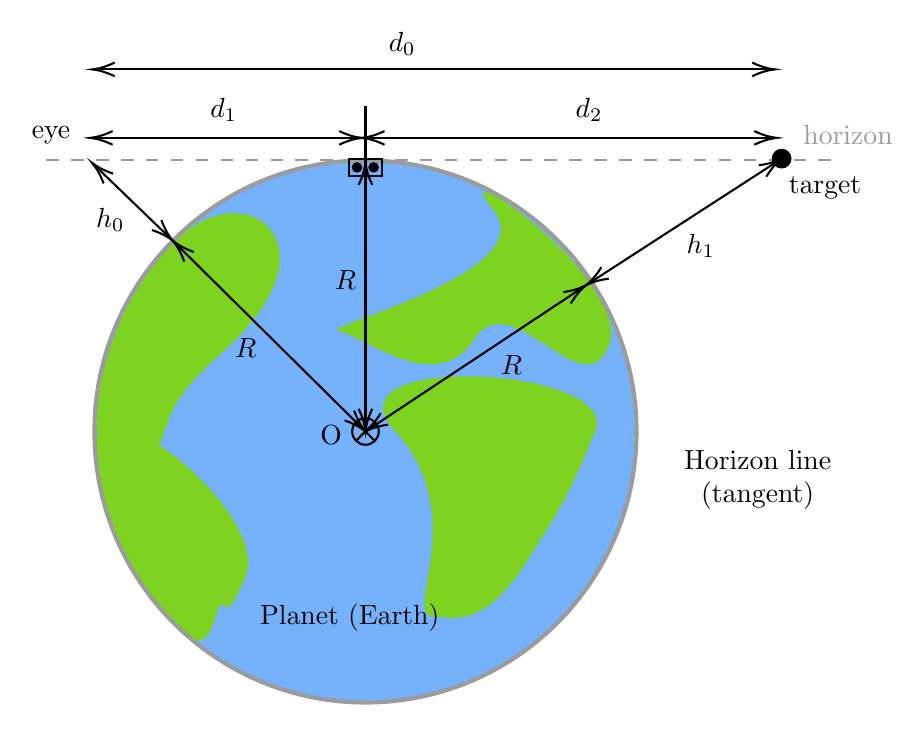
\begin{tikzpicture}[x=0.75pt,y=0.75pt,yscale=-1,xscale=1]
		%uncomment if require: \path (0,1046); %set diagram left start at 0, and has height of 1046
		
		%Shape: Circle [id:dp8762969614163911] 
		\draw  [draw opacity=0][fill={rgb, 255:red, 118; green, 177; blue, 251 }  ,fill opacity=1 ] (158.5,248.45) .. controls (158.5,176.79) and (216.59,118.7) .. (288.25,118.7) .. controls (359.91,118.7) and (418,176.79) .. (418,248.45) .. controls (418,320.11) and (359.91,378.2) .. (288.25,378.2) .. controls (216.59,378.2) and (158.5,320.11) .. (158.5,248.45) -- cycle ;
		%Shape: Polygon Curved [id:ds3774928120437888] 
		\draw  [draw opacity=0][fill={rgb, 255:red, 126; green, 211; blue, 33 }  ,fill opacity=1 ] (302.5,248.2) .. controls (266.5,209.2) and (411.5,217.2) .. (399,248) .. controls (386.5,278.8) and (382.5,285.2) .. (364.5,313.2) .. controls (346.5,341.2) and (331.5,339.2) .. (319.5,337.2) .. controls (307.5,335.2) and (338.5,287.2) .. (302.5,248.2) -- cycle ;
		%Shape: Polygon Curved [id:ds6073874191729449] 
		\draw  [draw opacity=0][fill={rgb, 255:red, 126; green, 211; blue, 33 }  ,fill opacity=1 ] (188.5,165.2) .. controls (220.5,125.2) and (257,146.4) .. (244.5,177.2) .. controls (232,208) and (201.5,217.2) .. (192.5,245.2) .. controls (183.5,273.2) and (172.5,267.2) .. (163.5,261.2) .. controls (154.5,255.2) and (156.5,205.2) .. (188.5,165.2) -- cycle ;
		%Shape: Polygon Curved [id:ds4494214746604088] 
		\draw  [draw opacity=0][fill={rgb, 255:red, 126; green, 211; blue, 33 }  ,fill opacity=1 ] (158.5,256.2) .. controls (155.5,219.2) and (243,287.4) .. (230.5,318.2) .. controls (218,349) and (221.5,319.2) .. (215.5,339.2) .. controls (209.5,359.2) and (200.5,345.2) .. (187.5,330.2) .. controls (174.5,315.2) and (161.5,293.2) .. (158.5,256.2) -- cycle ;
		%Shape: Polygon Curved [id:ds4760732148558635] 
		\draw  [draw opacity=0][fill={rgb, 255:red, 126; green, 211; blue, 33 }  ,fill opacity=1 ] (349.5,141.2) .. controls (323.5,110.2) and (418,176.4) .. (405.5,207.2) .. controls (393,238) and (358.5,176.2) .. (340.5,204.2) .. controls (322.5,232.2) and (287.5,202.2) .. (275.5,200.2) .. controls (263.5,198.2) and (375.5,172.2) .. (349.5,141.2) -- cycle ;
		%Shape: Circle [id:dp291125200889661] 
		\draw  [color={rgb, 255:red, 155; green, 155; blue, 155 }  ,draw opacity=1 ][line width=1.5]  (157.67,248.45) .. controls (157.67,176.34) and (216.14,117.87) .. (288.25,117.87) .. controls (360.36,117.87) and (418.83,176.34) .. (418.83,248.45) .. controls (418.83,320.56) and (360.36,379.02) .. (288.25,379.02) .. controls (216.14,379.02) and (157.67,320.56) .. (157.67,248.45) -- cycle ;
		%Flowchart: Summing Junction [id:dp06284611341095792] 
		\draw   (281.85,248.45) .. controls (281.85,244.92) and (284.72,242.05) .. (288.25,242.05) .. controls (291.78,242.05) and (294.65,244.92) .. (294.65,248.45) .. controls (294.65,251.98) and (291.78,254.85) .. (288.25,254.85) .. controls (284.72,254.85) and (281.85,251.98) .. (281.85,248.45) -- cycle ; \draw   (283.72,243.92) -- (292.78,252.98) ; \draw   (292.78,243.92) -- (283.72,252.98) ;
		%Straight Lines [id:da513650383675825] 
		\draw    (288.25,248.45) -- (288.25,91.4) ;
		%Straight Lines [id:da43410146667310356] 
		\draw    (288.25,120.7) -- (288.25,246.45) ;
		\draw [shift={(288.25,248.45)}, rotate = 270] [color={rgb, 255:red, 0; green, 0; blue, 0 }  ][line width=0.75]    (10.93,-3.29) .. controls (6.95,-1.4) and (3.31,-0.3) .. (0,0) .. controls (3.31,0.3) and (6.95,1.4) .. (10.93,3.29)   ;
		\draw [shift={(288.25,118.7)}, rotate = 90] [color={rgb, 255:red, 0; green, 0; blue, 0 }  ][line width=0.75]    (10.93,-3.29) .. controls (6.95,-1.4) and (3.31,-0.3) .. (0,0) .. controls (3.31,0.3) and (6.95,1.4) .. (10.93,3.29)   ;
		%Straight Lines [id:da48238029119566805] 
		\draw [color={rgb, 255:red, 155; green, 155; blue, 155 }  ,draw opacity=1 ] [dash pattern={on 4.5pt off 4.5pt}]  (134.5,117.6) -- (514.5,117.6) ;
		%Shape: Rectangle [id:dp030660008444230336] 
		\draw   (280.2,117.25) -- (288.12,117.25) -- (288.12,125.18) -- (280.2,125.18) -- cycle ;
		%Shape: Ellipse [id:dp7694022099033542] 
		\draw  [fill={rgb, 255:red, 0; green, 0; blue, 0 }  ,fill opacity=1 ] (282.13,121.22) .. controls (282.13,120.1) and (283.04,119.19) .. (284.16,119.19) .. controls (285.28,119.19) and (286.19,120.1) .. (286.19,121.22) .. controls (286.19,122.34) and (285.28,123.24) .. (284.16,123.24) .. controls (283.04,123.24) and (282.13,122.34) .. (282.13,121.22) -- cycle ;
		
		%Straight Lines [id:da9767109565484933] 
		\draw    (196.92,158.01) -- (286.83,247.04) ;
		\draw [shift={(288.25,248.45)}, rotate = 224.72] [color={rgb, 255:red, 0; green, 0; blue, 0 }  ][line width=0.75]    (10.93,-3.29) .. controls (6.95,-1.4) and (3.31,-0.3) .. (0,0) .. controls (3.31,0.3) and (6.95,1.4) .. (10.93,3.29)   ;
		\draw [shift={(195.5,156.6)}, rotate = 44.72] [color={rgb, 255:red, 0; green, 0; blue, 0 }  ][line width=0.75]    (10.93,-3.29) .. controls (6.95,-1.4) and (3.31,-0.3) .. (0,0) .. controls (3.31,0.3) and (6.95,1.4) .. (10.93,3.29)   ;
		%Straight Lines [id:da432947892630108] 
		\draw    (392.83,179.11) -- (289.92,247.34) ;
		\draw [shift={(288.25,248.45)}, rotate = 326.45] [color={rgb, 255:red, 0; green, 0; blue, 0 }  ][line width=0.75]    (10.93,-3.29) .. controls (6.95,-1.4) and (3.31,-0.3) .. (0,0) .. controls (3.31,0.3) and (6.95,1.4) .. (10.93,3.29)   ;
		\draw [shift={(394.5,178)}, rotate = 146.45] [color={rgb, 255:red, 0; green, 0; blue, 0 }  ][line width=0.75]    (10.93,-3.29) .. controls (6.95,-1.4) and (3.31,-0.3) .. (0,0) .. controls (3.31,0.3) and (6.95,1.4) .. (10.93,3.29)   ;
		%Straight Lines [id:da3451934890826034] 
		\draw    (194.06,155.21) -- (157.94,120.39) ;
		\draw [shift={(156.5,119)}, rotate = 43.95] [color={rgb, 255:red, 0; green, 0; blue, 0 }  ][line width=0.75]    (10.93,-3.29) .. controls (6.95,-1.4) and (3.31,-0.3) .. (0,0) .. controls (3.31,0.3) and (6.95,1.4) .. (10.93,3.29)   ;
		\draw [shift={(195.5,156.6)}, rotate = 223.95] [color={rgb, 255:red, 0; green, 0; blue, 0 }  ][line width=0.75]    (10.93,-3.29) .. controls (6.95,-1.4) and (3.31,-0.3) .. (0,0) .. controls (3.31,0.3) and (6.95,1.4) .. (10.93,3.29)   ;
		%Straight Lines [id:da851084269914018] 
		\draw    (487.07,118.09) -- (396.18,176.91) ;
		\draw [shift={(394.5,178)}, rotate = 327.09] [color={rgb, 255:red, 0; green, 0; blue, 0 }  ][line width=0.75]    (10.93,-3.29) .. controls (6.95,-1.4) and (3.31,-0.3) .. (0,0) .. controls (3.31,0.3) and (6.95,1.4) .. (10.93,3.29)   ;
		\draw [shift={(488.75,117)}, rotate = 147.09] [color={rgb, 255:red, 0; green, 0; blue, 0 }  ][line width=0.75]    (10.93,-3.29) .. controls (6.95,-1.4) and (3.31,-0.3) .. (0,0) .. controls (3.31,0.3) and (6.95,1.4) .. (10.93,3.29)   ;
		%Straight Lines [id:da07013991609200043] 
		\draw    (284.5,107) -- (157.5,107) ;
		\draw [shift={(155.5,107)}, rotate = 360] [color={rgb, 255:red, 0; green, 0; blue, 0 }  ][line width=0.75]    (10.93,-3.29) .. controls (6.95,-1.4) and (3.31,-0.3) .. (0,0) .. controls (3.31,0.3) and (6.95,1.4) .. (10.93,3.29)   ;
		\draw [shift={(286.5,107)}, rotate = 180] [color={rgb, 255:red, 0; green, 0; blue, 0 }  ][line width=0.75]    (10.93,-3.29) .. controls (6.95,-1.4) and (3.31,-0.3) .. (0,0) .. controls (3.31,0.3) and (6.95,1.4) .. (10.93,3.29)   ;
		%Straight Lines [id:da2114218008684503] 
		\draw    (484.5,107) -- (288.5,107) ;
		\draw [shift={(286.5,107)}, rotate = 360] [color={rgb, 255:red, 0; green, 0; blue, 0 }  ][line width=0.75]    (10.93,-3.29) .. controls (6.95,-1.4) and (3.31,-0.3) .. (0,0) .. controls (3.31,0.3) and (6.95,1.4) .. (10.93,3.29)   ;
		\draw [shift={(486.5,107)}, rotate = 180] [color={rgb, 255:red, 0; green, 0; blue, 0 }  ][line width=0.75]    (10.93,-3.29) .. controls (6.95,-1.4) and (3.31,-0.3) .. (0,0) .. controls (3.31,0.3) and (6.95,1.4) .. (10.93,3.29)   ;
		%Straight Lines [id:da565223458984289] 
		\draw    (483.5,74) -- (158.5,74) ;
		\draw [shift={(156.5,74)}, rotate = 360] [color={rgb, 255:red, 0; green, 0; blue, 0 }  ][line width=0.75]    (10.93,-3.29) .. controls (6.95,-1.4) and (3.31,-0.3) .. (0,0) .. controls (3.31,0.3) and (6.95,1.4) .. (10.93,3.29)   ;
		\draw [shift={(485.5,74)}, rotate = 180] [color={rgb, 255:red, 0; green, 0; blue, 0 }  ][line width=0.75]    (10.93,-3.29) .. controls (6.95,-1.4) and (3.31,-0.3) .. (0,0) .. controls (3.31,0.3) and (6.95,1.4) .. (10.93,3.29)   ;
		%Shape: Circle [id:dp13971582030925478] 
		\draw  [fill={rgb, 255:red, 0; green, 0; blue, 0 }  ,fill opacity=1 ] (484.5,117) .. controls (484.5,114.65) and (486.4,112.75) .. (488.75,112.75) .. controls (491.1,112.75) and (493,114.65) .. (493,117) .. controls (493,119.35) and (491.1,121.25) .. (488.75,121.25) .. controls (486.4,121.25) and (484.5,119.35) .. (484.5,117) -- cycle ;
		%Shape: Rectangle [id:dp4314405917477946] 
		\draw   (288.2,117.25) -- (296.12,117.25) -- (296.12,125.18) -- (288.2,125.18) -- cycle ;
		%Shape: Ellipse [id:dp8706822421069724] 
		\draw  [fill={rgb, 255:red, 0; green, 0; blue, 0 }  ,fill opacity=1 ] (290.13,121.22) .. controls (290.13,120.1) and (291.04,119.19) .. (292.16,119.19) .. controls (293.28,119.19) and (294.19,120.1) .. (294.19,121.22) .. controls (294.19,122.34) and (293.28,123.24) .. (292.16,123.24) .. controls (291.04,123.24) and (290.13,122.34) .. (290.13,121.22) -- cycle ;
		
		
		% Text Node
		\draw (236,330) node [anchor=north west][inner sep=0.75pt]   [align=left] {Planet (Earth)};
		% Text Node
		\draw (272,169.4) node [anchor=north west][inner sep=0.75pt]    {$R$};
		% Text Node
		\draw (212,86.4) node [anchor=north west][inner sep=0.75pt]    {$d_{1}$};
		% Text Node
		\draw (265,244) node [anchor=north west][inner sep=0.75pt]   [align=left] {O};
		% Text Node
		\draw (438,256) node [anchor=north west][inner sep=0.75pt]   [align=left] {\begin{minipage}[lt]{56.58pt}\setlength\topsep{0pt}
		\begin{center}
		Horizon line\\(tangent)
		\end{center}
		
		\end{minipage}};
		% Text Node
		\draw (298,54.4) node [anchor=north west][inner sep=0.75pt]    {$d_{0}$};
		% Text Node
		\draw (224,202.4) node [anchor=north west][inner sep=0.75pt]    {$R$};
		% Text Node
		\draw (352,210.4) node [anchor=north west][inner sep=0.75pt]    {$R$};
		% Text Node
		\draw (157,139.4) node [anchor=north west][inner sep=0.75pt]    {$h_{0}$};
		% Text Node
		\draw (441.5,151.9) node [anchor=north west][inner sep=0.75pt]    {$h_{1}$};
		% Text Node
		\draw (126,100) node [anchor=north west][inner sep=0.75pt]   [align=left] {eye};
		% Text Node
		\draw (388,86.4) node [anchor=north west][inner sep=0.75pt]    {$d_{2}$};
		% Text Node
		\draw (490.75,124.25) node [anchor=north west][inner sep=0.75pt]   [align=left] {target};
		% Text Node
		\draw (497.75,99.25) node [anchor=north west][inner sep=0.75pt]   [align=left] {\textcolor[rgb]{0.61,0.61,0.61}{horizon}};
		
		\end{tikzpicture}
		\vspace*{3mm}
		\caption[]{Visual Horizon configuration experience}	
	\end{figure}
	The application of Pythagoras gives us immediately:
	
	and:
	
	So let us compare the value of $d_1$ just obtained above (straight distance) for $d$ obtained previously that is the curvilinear distance:
	\begin{table}[H]
	\begin{center}
		\definecolor{gris}{gray}{0.85}
			\begin{tabular}{|c|c|c|}
				\hline
				\multicolumn{1}{c}{\cellcolor[gray]{0.75}\textbf{Altitude $h$ [m]}} & 
\multicolumn{1}{c}{\cellcolor[gray]{0.75}\textbf{Horizon distance $d$ [km]}}  & 
\multicolumn{1}{c}{\cellcolor[gray]{0.75}\textbf{Horizon distance $d_1$ [km]}} \\ \hline
		$1.5$ & $4.374$ & $4.374$\\ \hline
		$5$ & $7.98$ & $7.98$ \\ \hline
		$10$ & $11.29$ & $11.29$ \\ \hline
		$50$ & $25.25$ & $25.25$ \\ \hline
		$100$ & $35.71$ & $35.71$ \\ \hline
		$200$ & $50.51$ & $50.50$ \\ \hline
		$400$ & $71.43$ & $71.43$ \\ \hline
		$600$ & $87.48$ & $87.48$\\ \hline
		$800$ & $101.01$ & $101.02$\\ \hline
		$1,000$ & $112.93$ & $112.94$ \\ \hline
		$2,000$ & $159.70$ & $159.73$\\ \hline
		$3,000$ & $195.58$ & $195.64$\\ \hline
		$4,000$ & $225.83$ & $225.92$ \\ \hline
		$5,000$ & $252.47$ & $252.59$\\ \hline
		$10,000$ & $356.93$ & $357.29$ \\ \hline
	\end{tabular}
	\end{center}
	\caption{Visual horizon curvilinear and straight distance in function of the altitude}
	\end{table}
	So the bias of the people that believe that the Earth (and all other planets) is flat ("flat Earthers") is that when they do the experiments to prove their arguments they forget the "perfectly spheric" assumption of that model. Indeed as we have seen in the section of Astronomy the Earth's shape is more like a irregular potatoes and is locally (at human scale, i.e. a few hundreds of kilometres sometimes) absolutely not spherical due to relief irregularities.
	\begin{figure}[H]
		\centering
		\resizebox{\textwidth}{!}{
		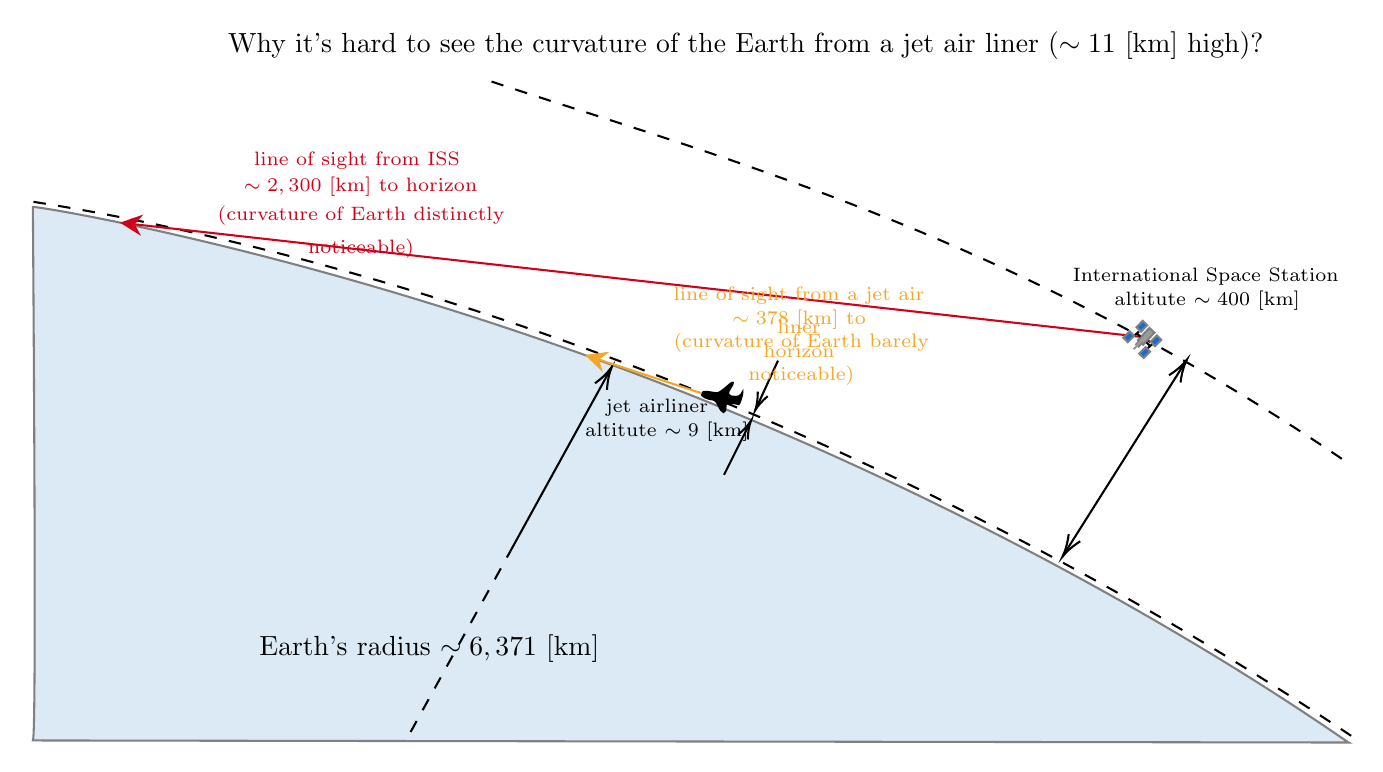
\begin{tikzpicture}[x=0.75pt,y=0.75pt,yscale=-1,xscale=1]
		%uncomment if require: \path (0,765); %set diagram left start at 0, and has height of 765
		
		%Shape: Polygon Curved [id:ds7456032244078723] 
		\draw  [color={rgb, 255:red, 128; green, 128; blue, 128 }  ,draw opacity=1 ][fill={rgb, 255:red, 219; green, 234; blue, 245 }  ,fill opacity=1 ] (19.37,123.91) .. controls (19.37,122.91) and (179.37,148.91) .. (359.37,223.91) .. controls (539.37,298.91) and (652.37,381.91) .. (653.37,381.91) .. controls (654.37,381.91) and (17.37,380.91) .. (19.37,380.91) .. controls (21.37,380.91) and (19.37,124.91) .. (19.37,123.91) -- cycle ;
		%Straight Lines [id:da7338812995983173] 
		\draw    (249.37,289.82) -- (297.41,202.58) ;
		\draw [shift={(298.37,200.82)}, rotate = 118.84] [color={rgb, 255:red, 0; green, 0; blue, 0 }  ][line width=0.75]    (10.93,-3.29) .. controls (6.95,-1.4) and (3.31,-0.3) .. (0,0) .. controls (3.31,0.3) and (6.95,1.4) .. (10.93,3.29)   ;
		%Straight Lines [id:da4993077705537168] 
		\draw  [dash pattern={on 4.5pt off 4.5pt}]  (201.37,376.82) -- (249.37,289.82) ;
		%Curve Lines [id:da4212994841399156] 
		\draw  [dash pattern={on 4.5pt off 4.5pt}]  (19.66,121.41) .. controls (132.37,138.91) and (386.37,199.91) .. (655.71,379.46) ;
		%Straight Lines [id:da5976261019382496] 
		\draw    (378.37,197.91) -- (368.21,220.1) ;
		\draw [shift={(367.37,221.91)}, rotate = 294.62] [color={rgb, 255:red, 0; green, 0; blue, 0 }  ][line width=0.75]    (8.74,-2.63) .. controls (5.56,-1.12) and (2.65,-0.24) .. (0,0) .. controls (2.65,0.24) and (5.56,1.12) .. (8.74,2.63)   ;
		%Straight Lines [id:da7935153526295384] 
		\draw    (352.37,252.91) -- (364.48,228.7) ;
		\draw [shift={(365.37,226.91)}, rotate = 116.57] [color={rgb, 255:red, 0; green, 0; blue, 0 }  ][line width=0.75]    (8.74,-2.63) .. controls (5.56,-1.12) and (2.65,-0.24) .. (0,0) .. controls (2.65,0.24) and (5.56,1.12) .. (8.74,2.63)   ;
		%Shape: Polygon Curved [id:ds2848990448309481] 
		\draw  [fill={rgb, 255:red, 0; green, 0; blue, 0 }  ,fill opacity=1 ] (356.62,208.62) .. controls (356.87,209.62) and (353.62,212.82) .. (354.37,214.12) .. controls (355.12,215.41) and (355.37,215.12) .. (358.12,215.41) .. controls (360.87,215.71) and (361.37,212.16) .. (361.12,213.91) .. controls (360.87,215.66) and (359.62,219.16) .. (359.37,218.91) .. controls (359.12,218.66) and (356.12,218.16) .. (354.12,218.16) .. controls (352.12,218.16) and (353.87,222.66) .. (352.12,222.66) .. controls (350.37,222.66) and (349.61,216.91) .. (347.12,216.66) .. controls (344.64,216.42) and (341.12,215.16) .. (341.62,213.66) .. controls (342.12,212.16) and (346.37,213.37) .. (348.62,213.66) .. controls (350.87,213.96) and (356.37,207.62) .. (356.62,208.62) -- cycle ;
		%Curve Lines [id:da6890853817208413] 
		\draw  [dash pattern={on 4.5pt off 4.5pt}]  (240.37,63.46) .. controls (348.37,99.46) and (489.37,136.46) .. (650.37,245.46) ;
		%Straight Lines [id:da5997220346582786] 
		\draw [color={rgb, 255:red, 208; green, 2; blue, 27 }  ,draw opacity=1 ]   (64.35,131.79) -- (552.98,186.44) ;
		\draw [shift={(61.37,131.46)}, rotate = 6.38] [fill={rgb, 255:red, 208; green, 2; blue, 27 }  ,fill opacity=1 ][line width=0.08]  [draw opacity=0] (10.72,-5.15) -- (0,0) -- (10.72,5.15) -- (7.12,0) -- cycle    ;
		%Straight Lines [id:da6377542681800714] 
		\draw [color={rgb, 255:red, 245; green, 166; blue, 35 }  ,draw opacity=1 ]   (288.22,196.12) -- (341.62,213.66) ;
		\draw [shift={(285.37,195.19)}, rotate = 18.18] [fill={rgb, 255:red, 245; green, 166; blue, 35 }  ,fill opacity=1 ][line width=0.08]  [draw opacity=0] (10.72,-5.15) -- (0,0) -- (10.72,5.15) -- (7.12,0) -- cycle    ;
		%Straight Lines [id:da33958695069390865] 
		\draw    (516.44,290.77) -- (574.3,199.15) ;
		\draw [shift={(575.37,197.46)}, rotate = 122.28] [color={rgb, 255:red, 0; green, 0; blue, 0 }  ][line width=0.75]    (10.93,-3.29) .. controls (6.95,-1.4) and (3.31,-0.3) .. (0,0) .. controls (3.31,0.3) and (6.95,1.4) .. (10.93,3.29)   ;
		\draw [shift={(515.37,292.46)}, rotate = 302.28] [color={rgb, 255:red, 0; green, 0; blue, 0 }  ][line width=0.75]    (10.93,-3.29) .. controls (6.95,-1.4) and (3.31,-0.3) .. (0,0) .. controls (3.31,0.3) and (6.95,1.4) .. (10.93,3.29)   ;
		%Shape: Rectangle [id:dp5721328294026073] 
		\draw  [color={rgb, 255:red, 128; green, 128; blue, 128 }  ,draw opacity=1 ][fill={rgb, 255:red, 155; green, 155; blue, 155 }  ,fill opacity=1 ] (559.73,184.44) -- (554.28,190.25) -- (551.85,187.97) -- (557.3,182.16) -- cycle ;
		%Shape: Rectangle [id:dp9568629406322029] 
		\draw  [color={rgb, 255:red, 128; green, 128; blue, 128 }  ,draw opacity=1 ][fill={rgb, 255:red, 155; green, 155; blue, 155 }  ,fill opacity=1 ] (553.75,189.36) -- (552.12,191.11) -- (550.99,190.05) -- (552.63,188.3) -- cycle ;
		%Straight Lines [id:da30610879594380047] 
		\draw [color={rgb, 255:red, 155; green, 155; blue, 155 }  ,draw opacity=1 ]   (555.48,186.19) -- (549.73,192.44) ;
		%Straight Lines [id:da478232566592679] 
		\draw    (551.14,184.66) -- (552.98,186.44) ;
		%Straight Lines [id:da36507063045616395] 
		\draw    (555.89,189.16) -- (557.73,190.94) ;
		%Straight Lines [id:da9054025117371924] 
		\draw    (549.98,185.94) -- (552.23,183.94) ;
		%Straight Lines [id:da7915605828727252] 
		\draw    (556.48,191.94) -- (558.73,189.94) ;
		%Shape: Rectangle [id:dp9269877374841] 
		\draw  [color={rgb, 255:red, 128; green, 128; blue, 128 }  ,draw opacity=1 ][fill={rgb, 255:red, 16; green, 107; blue, 221 }  ,fill opacity=1 ] (544.8,186.89) -- (547.85,183.82) -- (549.98,185.94) -- (546.92,189.01) -- cycle ;
		%Shape: Rectangle [id:dp6230756903193526] 
		\draw  [color={rgb, 255:red, 128; green, 128; blue, 128 }  ,draw opacity=1 ][fill={rgb, 255:red, 16; green, 107; blue, 221 }  ,fill opacity=1 ] (551.1,181.82) -- (554.16,178.75) -- (556.28,180.87) -- (553.23,183.94) -- cycle ;
		%Shape: Rectangle [id:dp2597661243321725] 
		\draw  [color={rgb, 255:red, 128; green, 128; blue, 128 }  ,draw opacity=1 ][fill={rgb, 255:red, 16; green, 107; blue, 221 }  ,fill opacity=1 ] (552.42,194.51) -- (555.48,191.44) -- (557.61,193.56) -- (554.55,196.62) -- cycle ;
		%Shape: Rectangle [id:dp5984182675319192] 
		\draw  [color={rgb, 255:red, 128; green, 128; blue, 128 }  ,draw opacity=1 ][fill={rgb, 255:red, 16; green, 107; blue, 221 }  ,fill opacity=1 ] (557.85,188.82) -- (560.91,185.75) -- (563.03,187.87) -- (559.98,190.94) -- cycle ;
		
		
		% Text Node
		\draw (112,38) node [anchor=north west][inner sep=0.75pt]   [align=left] {Why it's hard to see the curvature of the Earth from a jet air liner ($\displaystyle \sim 11$ [km] high)?};
		% Text Node
		\draw (127,328.55) node [anchor=north west][inner sep=0.75pt]   [align=left] {Earth's radius $\displaystyle \sim 6,371$ [km]};
		% Text Node
		\draw (317,161) node [anchor=north west][inner sep=0.75pt]  [color={rgb, 255:red, 245; green, 166; blue, 35 }  ,opacity=1 ] [align=left] {\begin{minipage}[lt]{105pt}\setlength\topsep{0pt}
		\begin{center}
		{\scriptsize line of sight from a jet air liner}
		\end{center}
		
		\end{minipage}};
		% Text Node
		\draw (124,96) node [anchor=north west][inner sep=0.75pt]  [color={rgb, 255:red, 208; green, 2; blue, 27 }  ,opacity=1 ] [align=left] {\begin{minipage}[lt]{75pt}\setlength\topsep{0pt}
		\begin{center}
		{\scriptsize line of sight from ISS}
		\end{center}
		
		\end{minipage}};
		% Text Node
		\draw (294,214.91) node [anchor=north west][inner sep=0.75pt]   [align=left] {{\scriptsize jet airliner}};
		% Text Node
		\draw (519,151.91) node [anchor=north west][inner sep=0.75pt]   [align=left] {{\scriptsize International Space Station}};
		% Text Node
		\draw (119,108) node [anchor=north west][inner sep=0.75pt]  [color={rgb, 255:red, 208; green, 2; blue, 27 }  ,opacity=1 ] [align=left] {\begin{minipage}[lt]{85pt}\setlength\topsep{0pt}
		\begin{center}
		{\scriptsize $\displaystyle \sim 2,300$ [km] to horizon}
		\end{center}
		
		\end{minipage}};
		% Text Node
		\draw (86,122) node [anchor=north west][inner sep=0.75pt]  [color={rgb, 255:red, 208; green, 2; blue, 27 }  ,opacity=1 ] [align=left] {\begin{minipage}[lt]{135pt}\setlength\topsep{0pt}
		\begin{center}
		{\scriptsize (curvature of Earth distinctly noticeable)}
		\end{center}
		
		\end{minipage}};
		% Text Node
		\draw (284,225.91) node [anchor=north west][inner sep=0.75pt]   [align=left] {{\scriptsize altitute $\displaystyle \sim 9$ [km]}};
		% Text Node
		\draw (539,162.91) node [anchor=north west][inner sep=0.75pt]   [align=left] {{\scriptsize altitute $\displaystyle \sim 400$ [km]}};
		% Text Node
		\draw (337,172) node [anchor=north west][inner sep=0.75pt]  [color={rgb, 255:red, 245; green, 166; blue, 35 }  ,opacity=1 ] [align=left] {\begin{minipage}[lt]{75pt}\setlength\topsep{0pt}
		\begin{center}
		{\scriptsize $\displaystyle \sim 378$ [km] to horizon}
		\end{center}
		
		\end{minipage}};
		% Text Node
		\draw (308,183) node [anchor=north west][inner sep=0.75pt]  [color={rgb, 255:red, 245; green, 166; blue, 35 }  ,opacity=1 ] [align=left] {\begin{minipage}[lt]{120.18pt}\setlength\topsep{0pt}
		\begin{center}
		{\scriptsize (curvature of Earth barely noticeable)}
		\end{center}
		\end{minipage}};
		\end{tikzpicture}
		}
		\caption{Earth's curvature visibility}
	\end{figure}
	Anyway an another argument is that we can prove with Isoperimetric Inequality that natural final shape for a cloud of dust is a sphere and otherwise that the acceleration of objects that fall all respect Newton's law in it's... spherical form! And also... if the Earth was flat... nobody so far as we know has seen it's border...
	
	Therefore the two relations to remember are:
	
	Keep in mind that these results are for a perfect sphere in vacuum. When an atmosphere exist, refraction effect (see proof in the section of Optics at page ) can drastically increase the distances with theoreticaly almost no limit. The picture below show the island Corse seen from Nice (in France) in very special winter conditions however the both places are distance of $210$ kilometers.
	
	
	
	\pagebreak
	\subsection{Wind direction}
	We will now prove mathematically something quite intuitive: the winds are moving from high to low pressure (it's silly like that but we must still prove it!).

	We know (\SeeChapter{see section Continuum Mechanics page \pageref{pressure}}) that the pressure force exerted on a surface $S$ is normal to this surface and is equal in scalar form to $P\cdot S$.
	
	For an air parcel volume $\mathrm{d}V=\delta x\delta y\delta z$ the total pressure force in the $x$ direction is then:
	
	\begin{figure}[H]
		\centering
		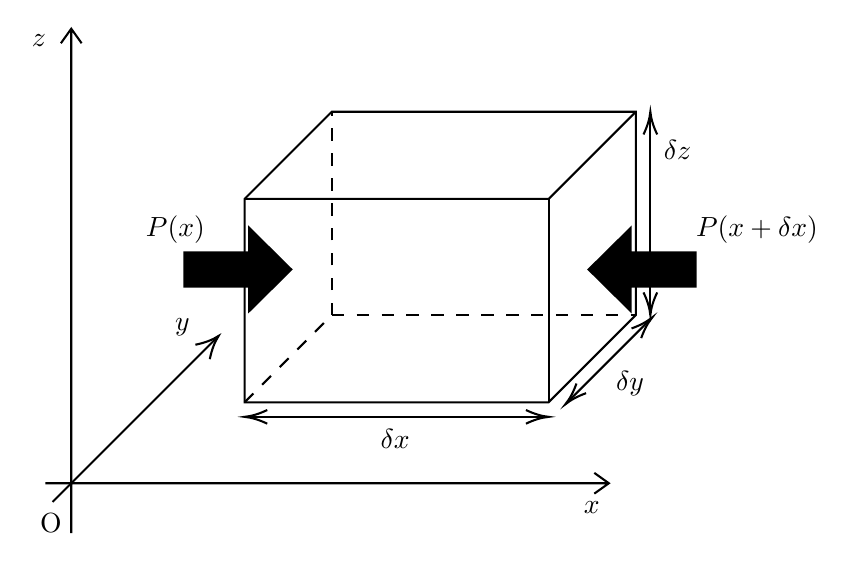
\begin{tikzpicture}[x=0.75pt,y=0.75pt,yscale=-1,xscale=1]
		%uncomment if require: \path (0,1046); %set diagram left start at 0, and has height of 1046
		
		%Shape: Axis 2D [id:dp8509758756050412] 
		\draw  (155,285) -- (426.5,285)(167.5,66) -- (167.5,309) (419.5,280) -- (426.5,285) -- (419.5,290) (162.5,73) -- (167.5,66) -- (172.5,73)  ;
		%Straight Lines [id:da8139122219497079] 
		\draw    (158.5,294) -- (237.09,215.41) ;
		\draw [shift={(238.5,214)}, rotate = 135] [color={rgb, 255:red, 0; green, 0; blue, 0 }  ][line width=0.75]    (10.93,-4.9) .. controls (6.95,-2.3) and (3.31,-0.67) .. (0,0) .. controls (3.31,0.67) and (6.95,2.3) .. (10.93,4.9)   ;
		%Shape: Cube [id:dp584915184532649] 
		\draw   (251,148) -- (293,106) -- (439.5,106) -- (439.5,204) -- (397.5,246) -- (251,246) -- cycle ; \draw   (439.5,106) -- (397.5,148) -- (251,148) ; \draw   (397.5,148) -- (397.5,246) ;
		%Straight Lines [id:da5325328735460306] 
		\draw  [dash pattern={on 4.5pt off 4.5pt}]  (251,246) -- (293,204) ;
		%Straight Lines [id:da6106666324703507] 
		\draw  [dash pattern={on 4.5pt off 4.5pt}]  (293,204) -- (439.5,204) ;
		%Straight Lines [id:da04045978174809162] 
		\draw  [dash pattern={on 4.5pt off 4.5pt}]  (293,204) -- (293,106) ;
		%Straight Lines [id:da2438045083528977] 
		\draw    (253,253) -- (395.5,253) ;
		\draw [shift={(397.5,253)}, rotate = 180] [color={rgb, 255:red, 0; green, 0; blue, 0 }  ][line width=0.75]    (10.93,-3.29) .. controls (6.95,-1.4) and (3.31,-0.3) .. (0,0) .. controls (3.31,0.3) and (6.95,1.4) .. (10.93,3.29)   ;
		\draw [shift={(251,253)}, rotate = 0] [color={rgb, 255:red, 0; green, 0; blue, 0 }  ][line width=0.75]    (10.93,-3.29) .. controls (6.95,-1.4) and (3.31,-0.3) .. (0,0) .. controls (3.31,0.3) and (6.95,1.4) .. (10.93,3.29)   ;
		%Straight Lines [id:da49089058431912114] 
		\draw    (406.91,245.59) -- (446.09,206.41) ;
		\draw [shift={(447.5,205)}, rotate = 135] [color={rgb, 255:red, 0; green, 0; blue, 0 }  ][line width=0.75]    (10.93,-3.29) .. controls (6.95,-1.4) and (3.31,-0.3) .. (0,0) .. controls (3.31,0.3) and (6.95,1.4) .. (10.93,3.29)   ;
		\draw [shift={(405.5,247)}, rotate = 315] [color={rgb, 255:red, 0; green, 0; blue, 0 }  ][line width=0.75]    (10.93,-3.29) .. controls (6.95,-1.4) and (3.31,-0.3) .. (0,0) .. controls (3.31,0.3) and (6.95,1.4) .. (10.93,3.29)   ;
		%Straight Lines [id:da5973407931031283] 
		\draw    (446.5,108) -- (446.5,202) ;
		\draw [shift={(446.5,204)}, rotate = 270] [color={rgb, 255:red, 0; green, 0; blue, 0 }  ][line width=0.75]    (10.93,-3.29) .. controls (6.95,-1.4) and (3.31,-0.3) .. (0,0) .. controls (3.31,0.3) and (6.95,1.4) .. (10.93,3.29)   ;
		\draw [shift={(446.5,106)}, rotate = 90] [color={rgb, 255:red, 0; green, 0; blue, 0 }  ][line width=0.75]    (10.93,-3.29) .. controls (6.95,-1.4) and (3.31,-0.3) .. (0,0) .. controls (3.31,0.3) and (6.95,1.4) .. (10.93,3.29)   ;
		%Right Arrow [id:dp8090868166631324] 
		\draw  [fill={rgb, 255:red, 0; green, 0; blue, 0 }  ,fill opacity=1 ] (222,173.8) -- (253.27,173.8) -- (253.27,162) -- (273.5,182) -- (253.27,202) -- (253.27,190.2) -- (222,190.2) -- cycle ;
		%Right Arrow [id:dp853942530096566] 
		\draw  [fill={rgb, 255:red, 0; green, 0; blue, 0 }  ,fill opacity=1 ] (468.27,190.2) -- (437,190.2) -- (437,202) -- (416.77,182) -- (437,162) -- (437,173.8) -- (468.27,173.8) -- cycle ;
		
		% Text Node
		\draw (147,67.4) node [anchor=north west][inner sep=0.75pt]    {$z$};
		% Text Node
		\draw (413,292.4) node [anchor=north west][inner sep=0.75pt]    {$x$};
		% Text Node
		\draw (216,204.4) node [anchor=north west][inner sep=0.75pt]    {$y$};
		% Text Node
		\draw (151,298) node [anchor=north west][inner sep=0.75pt]   [align=left] {O};
		% Text Node
		\draw (315,257.4) node [anchor=north west][inner sep=0.75pt]    {$\delta x$};
		% Text Node
		\draw (428.5,229.4) node [anchor=north west][inner sep=0.75pt]    {$\delta y$};
		% Text Node
		\draw (451.5,118.4) node [anchor=north west][inner sep=0.75pt]    {$\delta z$};
		% Text Node
		\draw (202,154.4) node [anchor=north west][inner sep=0.75pt]    {$P( x)$};
		% Text Node
		\draw (467,154.4) node [anchor=north west][inner sep=0.75pt]    {$P( x+\delta x)$};
		
		\end{tikzpicture}
	\end{figure}
	In addition, we have (\SeeChapter{see section Differential and  Integral Calculus page \pageref{differential calculus}}):
	
	Therefore:
	
	The mass pressure force is then:
	We can do the same calculation following $y$. Finally, the massic horizontal pressure force is given by:
	
	Thus, the pressure force (massic or not) is opposite to the horizontal gradient. The transmission of information (of the force) is done at the speed of sound for this equation (which explains the speed of air calls in your home or apartment and then force that can make slam doors or window).

It is therefore:

	\begin{itemize}
		\item  Directed from high to low pressure, perpendicular to the isobars

		\item Inversely proportional to the spacing of the isobars.
	\end{itemize}
	If we measure the values of the atmospheric pressure at different points of the globe and we connect between them the points of same pressure on a drawing, we get a series of curves, named "\NewTerm{isobars}\index{isobars}". The wind is directly determined by the atmospheric relief since it is a movement of air between the high to low pressure.

	The wind speed is then determined by the pressure gradient: that is, if the atmospheric pressure changes rapidly with distance, the wind blows strong, while it will be low in abarometric  "swamp" where this pressure remains almost unchanged on great distances. In summary, more the isobars are close together, more the wind will blow strong.

	The isobars are traditionally marked with a pitch of $5$ millibars on weather maps such as shown in the example below:
	\begin{figure}[H]
		\centering
		\includegraphics{img/engineering/depression.jpg}	
		\caption{Typical representation of isobars (on a depression)}
	\end{figure}
	Charts showing isobars are useful because they identify features such as anticyclones (areas of high pressure) and depressions (areas of low pressure).

	Areas of high and low pressure are caused by ascending and descending air. As air warms, it ascends leading to low pressure at the surface. As air cools, it descends leading to high pressure at the surface. This is illustrated in the diagram below.
	\begin{figure}[H]
		\centering
		\includegraphics{img/engineering/pressure_sytem.jpg}	
		\caption{High and low pressure systems}
	\end{figure}
	In general, low pressure leads to unsettled weather conditions and high pressure leads to settled weather conditions.

	In an anticyclone (high pressure) the winds tend to be light and blow in a clockwise direction (in the northern hemisphere as we will prove it later below). Also the air is descending, which reduces the formation of cloud and leads to light winds and settled weather conditions.

	In a depression (low pressure), air is rising and blows in an anticlockwise direction around the low (in the northern hemisphere). As it rises and cools, water vapour condenses to form clouds and perhaps precipitation. This is why the weather in a depression is often unsettled - there are usually frontal systems associated with depressions.
	
	To close this topic about winds, let us notice that meteorologists empirically defined (that is fun for the general culture) a unit of wind measurement that is just a match between the wind force and the distance between two isobars in steps of $5$ by $5$ [mb]:
	\begin{table}[H]
		\begin{center}
		\definecolor{gris}{gray}{0.85}
		\begin{tabular}{|l||c|c|}
			\hline
			{\cellcolor[gray]{0.75}\textbf{Distance between isobares} [km]} & {\cellcolor[gray]{0.75}\textbf{Unit} [Beaufort]} & {\cellcolor[gray]{0.75}\textbf{Speed} $[\text{m}\cdot \text{s}^{-1}]$}  \\ \hline
			$600$ (light breeze) & $2$ & $1.6$-$3.3$\\ \hline
			$500$ (average breeze) & $4$ & $3.4$-$5.4$\\ \hline
			$400$ (cold breeze) & $5$ & $8$-$10.7$\\ \hline
			$300$ (strong wind) & $6$ & $10.8$-$13.8$\\ \hline
			$200$ (big wind) & $7$ & $13.9$-$17.1$\\ \hline
			$100$ (storm) & $9$ & $20.8$-$24.4$\\ \hline
		\end{tabular}
		\end{center}
		\caption{Distance between isobars and wind speed (Beaufort units)}
	\end{table}
	
	\subsection{Atmospheric Profile Models}
	An atmospheric profile model is a mathematical model constructed to predict the profile of temperature, pressure or other in the atmosphere, locally depending on the measured height supposing a steady state of the atmosphere (same as if we take out a cylinder piece of the atmosphere and freeze time to analyse some of the properties of the atmosphere inside depending on the height in the cylinder). 

	There a lot of models but let us see just two easy one:
	
	\subsubsection{Atmospheric Exponential Profile Model}
	Consider that the atmosphere is a perfect fluid in a uniform gravity field. Then from the following Bernoulli's theorem relation, proved in the section of Continuum Mechanics (static fluid at page \pageref{Bernoulli theorem}):
	
	It comes then:
	
	Thus, to know the variation of pressure depending on height in the atmosphere or depth in the ocean, we have taken as hypothesis the "\NewTerm{hydrostatic equilibrium}\index{hydrostatic equilibrium}", that is the variation of pressure with height / depth is proportional to the gravity and density of the fluid.
	
	This is obviously not valid in the case of rapid movements of convection, like thunderstorms, but can easily be satisfied for slow movements (quasi-static) and at large scale: the "\NewTerm{synoptic scale}\index{synoptic scale}" ($2,000$-$20,000$ [km]).
	\begin{figure}[H]
		\begin{center}
			\includegraphics[scale=0.7]{img/engineering/meteoric_scale.jpg}
		\end{center}	
		\caption{Various meteorological scales}
	\end{figure}
	We will then combine this last relation with a state equation, such as that of the ideal gas at temperature $T$ and of density $\rho$ whose constituent particles have a mass $m$. So we have the ideal gas equation (\SeeChapter{see section Continuum Mechanics page \pageref{ideal gas law}}):
	
	with for recall $P$ that is the pressure expressed in Pascals, $V$ the volume in cubic meters, $R$ is the gas constant, $T$ is the temperature in Kelvin, $n$ the number of moles, $k$ is the Boltzmann constant, $\rho$ the particle density, $m$ the total mass of the particles.
	
	In the isothermal case (e.g. in the terrestrial stratosphere, above $10$ [km] altitude where the temperature is almost constant around $-55$ degrees Celsius), we found out easily by substitution that:
	
	Therefore, at a given pressure, the vertical pressure gradient is inversely proportional to temperature.

	Let us now consider the following relation:
	
	Using the exponential:
	
	The pressure therefore decreases exponentially with the altitude. $P_0$ being the pressure at ground level.

	Let us return to the relation:
	
	It can of course also be written as:
	
	which tells us that the distance $z$ between isobaric surfaces is directly proportional to temperature.

	We have also another common approach. Let us start again from the relation proved just earlier above, but for a mass $m$ of $1$ [kg]:
	
	and let us denote this relation as follow:
	
	Let us recall that (\SeeChapter{see section Differential and Integral Calculus page \pageref{usual derivatives}}):
	
	Therefore:	
	
	and now let assume that the temperature variation is linear in the atmosphere (which is not far from the truth for the first $10$ to $20$ km of the atmosphere such that:
	
	with $\lambda<0$ which is the temperature gradient in $[\text{K}\cdot\text{m}^{-1}]$.
	\begin{figure}[H]
		\centering
		\includegraphics[scale=0.4]{img/engineering/weather_temperature_pression_altitude_profile.jpg}	
		\caption[Typical profile of temperature and pressure on Earth]{Typical profile of temperature and pressure on Earth... late 120th century (source: ?)}
	\end{figure}
	Then we have:
	
	Therefore:
	
	Which gives:
	
	After simplification:
	
	Hence:
	
	Which can be written more aesthetically:
	
	A good practical example of application of this relation is the gliders and hang gliders. They expect the weather forecast that it communicates to them the height of the isotherm of zero degrees during its bulletins. They then deduce the temperature gradient per meter. For these athletes, good condition is to have a gradient of $1\;[^\circ \text{C}]$ by $100$ meters. It is therefore easy with the above relation to calculate the pressure at an altitude of $2,000$ meters and to derive the pressure gradient which allows them to use some the updrafts for their aerobatic practices.
	
	\subsubsection{Adiabatic Atmosphere Model}
	The adiabatic temperature gradient is, in the atmosphere, the air temperature change with altitude (i.e. the air temperature gradient), which only depends on the atmospheric pressure, that is to say:
	\begin{itemize}
		\item Without considering heat exchange with the environment (other air masses, relief, ground, etc.)

		\item  Without considering condensation (cloud formation) or precipitation.
	
		\item Without taking into account the Sun position and variations
	\end{itemize}
	This concept is of great importance in meteorology, as well as aviation and maritime navigation.

	We have proved in the section of Thermodynamics (see page \pageref{Laplace law thermodynamics}) the Laplace's thermodynamics law (satisfied under certain conditions!):
	
	with the Laplace coefficient:
	
	Therefore in massic form the Laplace's law becomes:
	
	We can take the logarithm:
	
	But by taking the logarithmic differential:
	
	We then have (relationship that we will reuse in the section of Music Mathematics)
	
	We could also have found this result directly from the relation proved in the section Thermodynamics:
	
	By taking also the logarithmic differential  of the ideal gas law where $n$ is, for recall, the number of moles (\SeeChapter{see section Continuum Mechanics page \pageref{ideal gas law}}):
	
	But in the massic form for one mole:
	
	where $M_m$ is the molar mass (\SeeChapter{see section Analytical Chemistry page \pageref{molar mass}}), we have:
		
	Therefore:
	
	We then get:
	
	Therefore:
	
	Let us use the relation proved earlier shown above:
	
	It comes then:
	
	So we have an atmosphere with constant and negative thermal gradient (temperature decreases linearly with altitude):
	
	The last form using the molar mass is more convenient because it allows to characterize the studied medium. Note that this is a model that looks to work well for an altitude of $0$ to $90$ [km] on Venus but much less well for the planet Earth.
	\begin{tcolorbox}[colframe=black,colback=white,sharp corners]
	\textbf{{\Large \ding{45}}Example:}\\\\
	We then have for example for Earth (thus knowing that the model is not well adapted):
	\begin{gather*}
		g\cong 9.81\;[\text{m}\cdot\text{s}^{-2}]\qquad R\cong 8.314\;[\text{J}\cdot \text{K}^{-1}\cdot \text{mol}^{-1}]
	\end{gather*}
	and the adiabatic coefficient for air is equal to $\gamma=1.4$, and its molecular weight:
	\begin{gather*}
		M_{m,\text{air}}\cong 28.96\cdot 10^{-3}\;[\text{kg}\cdot\text{mol}^{-1}]
	\end{gather*}
	Therefore:
	\begin{gather*}
		\kappa=-0.00976\;[\text{K}\cdot\text{m}^{-1}]\cong -1\;[\text{K}\cdot\text{hm}^{-1}]
	\end{gather*}
	which corresponds to the current idea: $1$ degree per $100$ meters.
	\end{tcolorbox}
	
	\pagebreak
	\paragraph{Hypsometric equation}\mbox{}\\\\
	The hypsometric equation, also known as the thickness equation, relates an atmospheric pressure ratio to the equivalent thickness of an atmospheric layer under the assumptions of constant temperature and gravity. It is derived from the hydrostatic equation and the ideal gas law.
	
	So we have just proved for to hydrostatic equilibrium:
	
	We can integrate this relationship if we know $T$ as a function of $P$ or $z$. The direct measurement of $P$ in practice is easier (single altimeters are actually barometers if they don't use GPS).

	We can then separate the variables:
	
	By integrating between two levels $a$ and $b$:
	
	Since:
	
	Then to continue we use a trick. We will define the average temperature by the relation:
	
	Which then allows us to write:
	
	Therefore:
	
	or written differently:
	
	or after rearrangement and change the notation for the average temperature:
	
	Both boxed relations are each respectively named "\NewTerm{hypsometric equation}\index{hypsometric equation}" (from the Greek "hypso" for "height").
	
	\pagebreak
	\subsection{Earth's equilibrium temperature}
	The "\NewTerm{planetary equilibrium temperature}\index{planetary equilibrium temperature}" is as we already know (\SeeChapter{see section Astronomy page \pageref{planetary equilibrium temperature}}) a theoretical temperature that a planet would be at when considered simply as if it were a black-body being heated only by its parent star. In this model, the presence or absence of an atmosphere (and therefore any greenhouse effect) is not considered, and one treats the theoretical black-body temperature as if it came from an idealized surface of the planet.

	Other authors use different names for this concept, such as "\NewTerm{equivalent black-body temperature of a planet}\index{equivalent black-body temperature of a planet}", or the "\NewTerm{effective radiation emission temperature of the planet}\index{effective radiation emission temperature of the planet}".

	If the incident solar radiation ("\NewTerm{insolation}\index{insolation}") - or incident power radiation - on the planet at its orbital distance from the Sun is $M_\odot$, the amount of energy absorbed by the planet ($\mathrm{d}\Phi/\mathrm{d}S$) will depend on its reflection coefficient (albedo $\rho$) and its cross-sectional area $S$ or average radius $R$ as:
	
	Note that the albedo would be zero for a black-body as we have seen it in the section of Optical Geometry. However, in planetology, more useful results are obtained by accounting for a measured or assumed planetary albedo $\rho>0$.

	The infrared power radiated by the planet as thermal radiation will depend on its emissivity and its surface area, according to the Stefan–Boltzmann equation proved in the section of Thermodynamics (see page \pageref{stefan boltzmann law}):
	
	and as it is a power by unit surface we will multiply it by the above surface area of the planet such that:
	
	 For a spherical planet, the surface of a perfect spherical area is well known (\SeeChapter{see section Geometric Shapes page \pageref{surface of a sphere}})! Therefore:
	
	But a planet that does not absorb all incident radiation (sometimes known as a grey body) emits less total energy than a black-body and is characterized by an emissivity, $\varepsilon< 1$, therefore (by definition emissivity + albedo = 1):
	
	The equilibrium temperature is then calculated by setting $P_\text{in}=P_\text{out}$. Thus:
	
	Therefore:
	
	It is interesting to note that the equilibrium temperature does not depend on the size of the planet, because both the incoming radiation and outgoing radiation depend on the area of the planet!
	
	Using a more astrophysical point of view if we don't know $M_\odot$, based on the luminosity $L_\odot$ (power) of the star and its distance $d$ to the planet we have as proved in the section of Astrophysics:
	
	Therefore:
	
	Earth's overall, average albedo is about $\rho\cong 0.31$ and the emissivity of Earth is considered as being about $\varepsilon\cong 0.96$ and $M_\odot\cong 1376$ [W$\cdot$m$^{-2}$].

	A numerical application for Earth gives $T_\text{eq}=253.7$ [K] (that is $-19.5$ [$^\circ$C]).

	Based on this calculation, Earth's expected average global temperature is well below the freezing point of water!

	Earth's actual average global temperature is around $14$ [$^\circ$C]. Our planet is warmer than predicted with  a pretty big difference!

	Why is Earth's temperature so much warmer than what our calculations predict? The answer is because certain gases in the atmosphere trap some extra heat, warming our planet like a blanket. This extra warming is named the "greenhouse effect" (see further below). Without it, our planet would be a frozen ball of ice. Thanks to the natural greenhouse effect, Earth is comfortable place for life as we know it. However, too much of a good thing can cause problems. In recent decades, a rise in the amount of greenhouse gases has begun to warm Earth a bit too much.
	
	\begin{tcolorbox}[title=Remark,arc=10pt,breakable,drop lifted shadow,
  skin=enhanced,
  skin first is subskin of={enhancedfirst}{arc=10pt,no shadow},
  skin middle is subskin of={enhancedmiddle}{arc=10pt,no shadow},
  skin last is subskin of={enhancedlast}{drop lifted shadow}]
	For extrasolar planets the temperature of the star can be calculated from the color of the star using Planck's law (\SeeChapter{see section Thermodynamics page \pageref{planck law}}). The calculated temperature of the star can be used with the Hertzsprung–Russell diagram (\SeeChapter{see section Astrophysics page \pageref{hertzsprung russell diagram}}) to determine the absolute magnitude of the star, which can then be used with observational data to determine the distance to the star and finally the size of the star. Orbital simulations are used to determine what orbital parameters (including orbital distance) produce the observations seen by astronomers. Astronomers use a hypothesized albedo and can then estimate the equilibrium temperature.
	\end{tcolorbox}
	
	\pagebreak
	\subsubsection{Greenhouse effect}\label{greenhouse effect}
	The greenhouse effect is the process by which radiation from a planet's atmosphere warms the planet's surface to a temperature above what it would be without its atmosphere.

	If a planet's atmosphere contains radiately active gases (i.e., greenhouse gases) the atmosphere will radiate energy in all directions. Part of this radiation is directed towards the surface, warming it. The downward component of this radiation – that is, the strength of the greenhouse effect – will depend on the atmosphere's temperature and on the amount of greenhouse gases that the atmosphere contains.

	Earth's natural greenhouse effect is critical to supporting life. Human activities, primarily the burning of fossil fuels and clearing of forests, have intensified the natural greenhouse effect, causing global warming.
	\begin{figure}[H]
		\begin{center}
			\includegraphics[scale=0.9]{img/engineering/greenhouse_effect.jpg}
		\end{center}	
		\caption{Greenhouse effect concept}
	\end{figure}
	For a mathematical analysis of the greenhouse effect we must improve our above model. Consider for this that we denote $T_S$ the temperature of surface of the Earth (or any other planet) and $T_A$ the temperature of its atmosphere.	The thermodynamic equilibrium of atmosphere gives us in the point of view of the radiation using again the Boltzmann law and considering that Earth's atmosphere radiates $50\%$ back in space and reflects back $50\%$ back to Earth surface (last measurements in the early 121st century - holocene calendar - gives $40\%$ reflected back!):
	
	Therefore it is immediate that:
	
	Remember now the equilibrium proved earlier:
	
	That simplifies to:
	
	Using our new notation:
	
	Therefore after rearranging:
	
	Now we add to this the back-radiation due to atmosphere:
	
	That is:
	
	Therefore after rearrangement:
	
	A numerical application gives $T_S\cong 297$ [K] that is $14$ [$^\circ$ C]. This is quite more accurate than the previous model!

	\subsubsection{Milankovitch cycles}\label{milankovic cycles}
	The Milankovitch cycles are periodic or quasiperiodic changes in the parameters of the Earth's orbit and tilt, which in turn affect the climate. The three major types of Milankovitch cycle are:
	\begin{itemize}
		\item changes in the eccentricity of the Earth's orbit
		\item changes in the obliquity, or tilt of the Earth's axis
		\item precession, meaning changes in the direction of the Earth's axis relative
to the fixed stars
	\end{itemize}
These changes do not affect the overall annual amount of solar radiation hitting the Earth, but they affect the strength of the seasons in different ways at different latitudes. It is widely believed that they are partially responsible for the glacial cycles. However, the details of how this occurs are complex and poorly understood.
	\begin{figure}[H]
		\begin{center}
			\includegraphics[scale=0.8]{img/engineering/milankovitch_cylces.jpg}
		\end{center}	
		\caption[Past and future Milankovitch cycles]{Past and future Milankovitch cycles (source: Wikipedia)}
	\end{figure}
	\begin{tcolorbox}[title=Remark,arc=10pt,breakable,drop lifted shadow,
  skin=enhanced,
  skin first is subskin of={enhancedfirst}{arc=10pt,no shadow},
  skin middle is subskin of={enhancedmiddle}{arc=10pt,no shadow},
  skin last is subskin of={enhancedlast}{drop lifted shadow}]
	By the mid-seventies the Earth’s orbital parameters were known over the last million years to a good accuracy thanks geological records. A decisive step was made by  André Berger (11978 according to holocene calendar), who expressed in an analytical form the Fourier decomposition of the Earth's orbital parameters relevant for the astronomical theory of palaeoclimates. This work constitutes the first demonstration that the spectrum of climatic precession is dominated by periods of $19,000$, $22,000$ and $24,000$ years, that of obliquity, by a period $41,000$ years, and eccentricity has periods of $400,000$ years, $125,000$ years and $96,000$ years. 
	\end{tcolorbox}
	
	For information, the rotation of Earth's on itself slows down at the day we write these lines of approximately $2.3$ milliseconds per century. That means $1$ hour every $180$ millions years. Each year the Earth's orbit speed around the Sun also slows down of approximately $3$ nanometers-per-second. Using Kepler's law, that means that the Earth goes further away from the Sun of $3$ micrometers per $1$ billion year......!!!!
	
	\subsection{Weather (sounding) balloon}
	A pretty interesting example of applied mathematics to weather engineering is the study of the famous weather balloons and especially the characteristic of their volume depending on the altitude which is often subject to debate in discussion groups when nobody formalizes the problem once and for all. You will therefore understand that this is what we will discuss here and especially we will try to determine the theoretical diameter thereof at a given altitude.
	\begin{figure}[H]
		\centering
		\includegraphics[scale=0.8]{img/engineering/weather_balloons.jpg}	
		\caption[]{Small weather balloon}
	\end{figure}
	The statement of the often discussed problem is the following:

	Given a PVC (Polyvinyl Chloride) weather balloon of mass $m$ used to take at high-altitude an apparatus for performing measurements. The envelope of the balloon contains $n$ moles of the hydrogen ideal gas thus having a molar mass:
	
	The atmosphere will be treated as a perfect gas, of average molecular weight:
	
	at N.T.P. (Normal conditions of Temperature and Pressure).

	We first we want to find what is the ascension force experienced by the balloon?

	Then we want to determine the minimum amount of material $n_0$ providing the take off of the balloon for a given total mass (including the balloon itself!) of $2.6$ [kg]. then the volume $V_0$ corresponding to the starting altitude.

	Let us recall two things first to solve this first point:
	\begin{enumerate}
		\item Any body immersed in a liquid (or gas) undergoes an upward force equal to the weight of the volume it displaces (Archimedes force) according to the relation proved in the section Continuum Mechanics:
		

		\item An ideal gas with a mass in grams equal to the molar mass occupies according to the ideal gas law a volume of $22.4$ [L] at $273.15$ [K] and at a pressure of $1$ [atm] as we have proved it in the section of Thermochemisty. Which gives at N.T.P:
		
	\end{enumerate}
	So for the balloon to fleet at constant height (without mounting but without falling too ...) with just sufficient quantity $n_0$ of hydrogen, it is necessary according to the Archimedes principle that the volume of air that it moves has a weight equal to the total mass of the balloon and the probe, thus $2.6$ [kg] in our case!

	So since $22$ [L] air weigh about $29$ grams, it is necessary that the volume that it moves to be equal to $2.6$ [kg] of air. Either by a simple rule of three:
	
	So if the balloon is spherical, it gives a radius of:
	
	Thus a diameter of about $1.56$ [m] at the ground. This is consistent with reality!

	We still need to determine the number of moles of hydrogen. It comes immediately:
	
	Now that we know the number of moles in the balloon , if we know the temperature and pressure at a height of $22,000$ [m] (typical altitude of a small weather balloon) it only remains to apply ideal gas law to determine the volume at this altitude then given by the relation proved in the section Continuum Mechanics:
	
	and at $22,000$ [m] above sea level, we have following the numerical tables available on the Internet:
	
	But because solar radiation is about $30\%$ higher in this altitude and the balloon is considered as adiabatic system (without heat exchange) and does not restore the power stored in the external environment. We consider that the temperature is at least $30\%$ higher which gives us such for values:
	
	
	We could also use (because of the adiabatic assumption) the Boyle's relation (\SeeChapter{see section Continuum Mechanics page \pageref{boyle mariotte law}}) to achieve the same result:
	
	This gives a radius of about $2.33$ [m] (thus diameter  of about $4.6$ [m]) instead of $0.78$ [m] to the ground! An increase of the diameter of about $300\%$. However, it is more important to focus on the increasing surface to determine the elastic stress forces on the PVC. So we have before:
	
	and after:
	
	Thus an increase of the surface of about $1,000\%$ while a standard elastomer (including PVC as a part) is not resistant to a relative change more than $500\%$ !!! It is then much easier to understand from the point of view of the surface, why the balloon does not withstand an increase in the diameter of about $300\%$.

	Moreover, if we apply a little abusively Hook's law to the balloon (\SeeChapter{see section Continuum Mechanics page \pageref{hooke law}}), with PVC Young's modulus which is between (source Wikipedia):
	
	We have:
	
	Which complies with the numeral data tables which gives an elastic lower limit value of $50$ [MPa] and an upper limit of $80$ [MPa] for PVC (source Wikipedia). We can then calculate the minimum and maximum theoretical height that the balloon can reach.

	So for the minimum height, we will write first:
	
	Which then corresponds to a final radius of:
	
	Which corresponds to a volume of:
	
	Applying Boyle-Martiotte:
	
	which is a pressure corresponding to a height of about $18,000$ [m] according to the experimental measurements (\url{www.engineeringtoolbox.com}) and this is indeed a rare height at which PVC balloons blow up.

	Now let us do the same with the maximum height:
	

	Which then corresponds to a final radius of:
	
	Which corresponds to a volume of:
	
	Applying Boyle-Martiotte:
	
	which is a pressure corresponding to a height of about $24,000$ [m] according to the experimental measurements and this is indeed a height at which the highest PVC balloons burst.
	
	\subsection{Cyclogenesis and Anticyclogenesis}
	Cyclogenesis is the development or strengthening of cyclonic circulation in the atmosphere (a low-pressure area). 
	
	Most of the atmospheric mass is contained within the first $20$ kilometres in altitude, so that the large-scale meteorology runs on a thin spherical shell (and can be assimilated to the mechanics of a two-dimensional fluid).

	The circulation engine of the atmosphere in the tropics is solar heating. Because of the inclination of $23.5$ degrees to the axis of rotation of the Earth, the Sun is never more than a few tenths of a degree from the zenith at noon throughout the year in the tropics, which gives maximum warming around the geographic equator.

	We must therefore distinguish air circulation in the vicinity of the tropics, characterized by strong vertical movement due to thermal convection, and circulation at mid-latitudes, made almost of horizontal movements:
	\begin{figure}[H]
		\centering
		\includegraphics[scale=1]{img/engineering/wind_circulation_earth.jpg}	
		\caption[Simplified schematic and idealized caricature of wind circulation on Earth]{Simplified schematic and idealized caricature of wind circulation on Earth (source: ?)}
	\end{figure}
	Let us suppose for a moment that we completely stopped the movement of the air in the atmosphere relatively to the surface of the planet, and that we leave it then start turning from West to East (left to right on the images) from the rest position. The pressure gradient force causes the air to move from high pressure areas to low pressure areas ("vacuum call"). These convective movements are named "\NewTerm{Hadley cells}\index{Hadley cells}".
	\begin{figure}[H]
		\begin{center}
			\includegraphics[scale=0.7]{img/engineering/hadley_and_ferrel_cells.jpg}
		\end{center}	
		\caption[Hadley and Ferrel cells]{Hadley and Ferrel cells (source: \url{www.climatica.org.uk})}
	\end{figure}
	However, when the rotation movement began the Coriolis force (due to the rotation of the Earth) deflects the North-South winds towards the West and South-North winds eastward for an observer falling in the North Pole (\SeeChapter{see section Classical Mechanics page \pageref{coriolis force}}). We see therefore the formation of cyclones turning in the opposite clockwise direction  in the Northern Hemisphere and vice versa in the Southern hemisphere (due to the direction of the vector $\vec{\omega}$ in this part of the hemisphere).
	
	The higher the air velocity increases, the more the Coriolis force increases accentuating the deviation. Eventually the Coriolis force reaches a value equal and opposite to that of the force of the pressure gradient, thus producing a flow of constant velocity (no acceleration), parallel to the isobars thus defining the geometric limit of the Hadley cell. This is what we name "\NewTerm{geostrophic balance}\index{geostrophic balance}". In practice, the flow outside the tropics is almost always in quasi-geostrophic equilibrium.

	In the absence of direct wind measurement, meteorologists can estimate the wind speed at a given point by measuring on a weather map the pressure gradient and the latitude. The geostrophic approximation is purely diagnostic. It has no predictive value because its equation contains no term of change depending on time.
	
	In the tropics, where the Coriolis force is becoming weaker until to be zero at the equator, there are other forces, such as centrifugal force, that balance the pressure gradient force.

	This is what we will prove here mathematically using Continuum Mechanics (fluids) and Classical Mechanics (see corresponding sections for the prerequisites).
	
	We know that in our system intervene pressure forces (gradient), centrifugal forces, gravity forces. Forces to which we must not forget to add the Coriolis force (implicitly its corresponding acceleration) of the system (meaning: the cyclone) with pulsation $\vec{\omega}$ (\SeeChapter{see section Classical Mechanics page \pageref{pulsation frequency period wave number}}):
	
	and the Coriolis force (implicitly: acceleration) of the fluid by unit mass (the reason for this unit choice will appear obvious few paragraphs further below) with respect to the pulsation $\vec\Omega$ of the Earth:
	
	Thus, as we know (\SeeChapter{see section Classical Mechanics page \pageref{coriolis force}}), the Coriolis force will tend to deflect any descending movement to the right (East) in the Northern Hemisphere and any ascending movement to the left (West) in the Southern hemisphere (following we place ourselves and look in the direction of fluid movement in the previous figures).

	This is why the air at the base of the Hadley cell, travelling at low altitude from the Tropic to the Equator will be deflected to the West to give the east trade winds.

	We have also proved in the section of Continuum Mechanics a particular form of the Euler equation of the second form (see page \pageref{Euler equation of the 2nd form}) that was:
	
	Rearranging this relation can also be written:
	
	But we had also proved that:
	
	It comes in the Earth reference frame:
	
	It is therefore of the equation defining the pressure within the fluid considered as isolated. In this relation, we must still subtract the Coriolis pressure  forces due to the geocentric reference frame to get the system the dynamic of the "cyclone":
	
	Which finally gives:
	
	\begin{figure}[H]
		\centering
		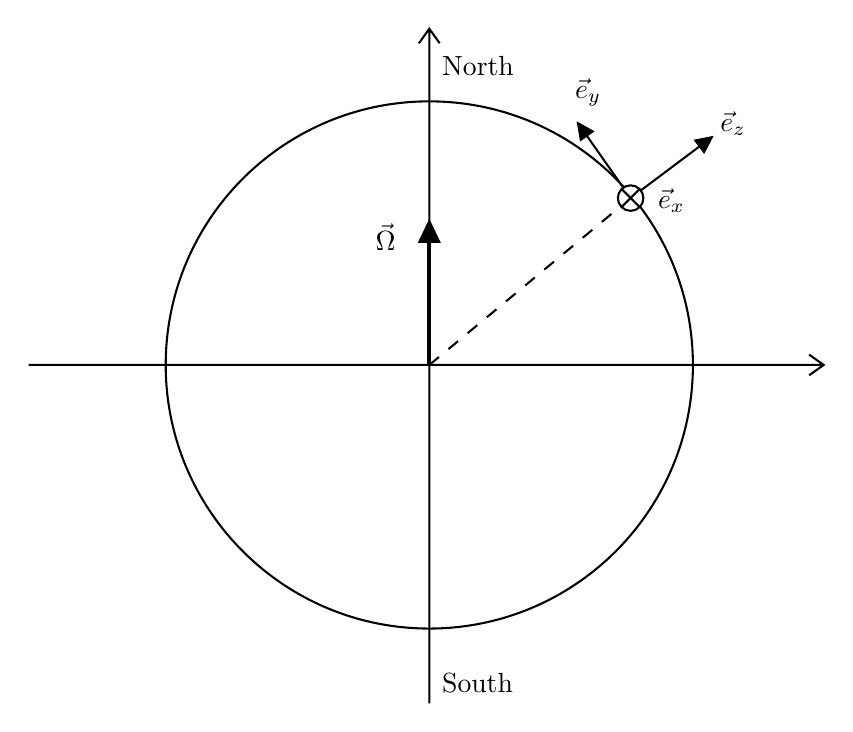
\begin{tikzpicture}[x=0.75pt,y=0.75pt,yscale=-1,xscale=1]
		%uncomment if require: \path (0,428); %set diagram left start at 0, and has height of 428
		
		%Shape: Axis 2D [id:dp17612767891069248] 
		\draw  (119.3,205) -- (502.3,205)(312.3,43) -- (312.3,368) (495.3,200) -- (502.3,205) -- (495.3,210) (307.3,50) -- (312.3,43) -- (317.3,50)  ;
		%Shape: Circle [id:dp19535863351599891] 
		\draw   (185.3,205) .. controls (185.3,134.86) and (242.16,78) .. (312.3,78) .. controls (382.44,78) and (439.3,134.86) .. (439.3,205) .. controls (439.3,275.14) and (382.44,332) .. (312.3,332) .. controls (242.16,332) and (185.3,275.14) .. (185.3,205) -- cycle ;
		%Straight Lines [id:da22593307304932297] 
		\draw [line width=1.5]    (312.3,204.6) -- (312.3,138.6) ;
		\draw [shift={(312.3,134.6)}, rotate = 90] [fill={rgb, 255:red, 0; green, 0; blue, 0 }  ][line width=0.08]  [draw opacity=0] (11.61,-5.58) -- (0,0) -- (11.61,5.58) -- cycle    ;
		%Straight Lines [id:da6400030790181344] 
		\draw  [dash pattern={on 4.5pt off 4.5pt}]  (312.3,205) -- (409.3,124.6) ;
		%Straight Lines [id:da16097150960526974] 
		\draw    (409.3,124.6) -- (385.02,90.05) ;
		\draw [shift={(383.3,87.6)}, rotate = 54.9] [fill={rgb, 255:red, 0; green, 0; blue, 0 }  ][line width=0.08]  [draw opacity=0] (8.93,-4.29) -- (0,0) -- (8.93,4.29) -- cycle    ;
		%Straight Lines [id:da18925972407001823] 
		\draw    (409.3,124.6) -- (446.9,96.4) ;
		\draw [shift={(449.3,94.6)}, rotate = 143.13] [fill={rgb, 255:red, 0; green, 0; blue, 0 }  ][line width=0.08]  [draw opacity=0] (8.93,-4.29) -- (0,0) -- (8.93,4.29) -- cycle    ;
		%Flowchart: Summing Junction [id:dp8079524044582922] 
		\draw  [fill={rgb, 255:red, 255; green, 255; blue, 255 }  ,fill opacity=1 ] (403.15,124.6) .. controls (403.15,121.2) and (405.9,118.45) .. (409.3,118.45) .. controls (412.7,118.45) and (415.45,121.2) .. (415.45,124.6) .. controls (415.45,128) and (412.7,130.75) .. (409.3,130.75) .. controls (405.9,130.75) and (403.15,128) .. (403.15,124.6) -- cycle ; \draw   (404.95,120.25) -- (413.65,128.95) ; \draw   (413.65,120.25) -- (404.95,128.95) ;
		
		% Text Node
		\draw (317,352) node [anchor=north west][inner sep=0.75pt]   [align=left] {South};
		% Text Node
		\draw (317,55) node [anchor=north west][inner sep=0.75pt]   [align=left] {North};
		% Text Node
		\draw (285,135.4) node [anchor=north west][inner sep=0.75pt]    {$\vec{\Omega }$};
		% Text Node
		\draw (381,65.4) node [anchor=north west][inner sep=0.75pt]    {$\vec{e}_{y}$};
		% Text Node
		\draw (451,81.4) node [anchor=north west][inner sep=0.75pt]    {$\vec{e}_{z}$};
		% Text Node
		\draw (421,118.4) node [anchor=north west][inner sep=0.75pt]    {$\vec{e}_{x}$};
		
		\end{tikzpicture}
		\vspace*{3mm}
		\caption[]{North-South slice of Earth for cyclogenesis study}
	\end{figure}
	If we zoom on the reference frame related to the cyclone and translate to it the vector pulse of the Earth, we have:
	\begin{figure}[H]
		\centering
		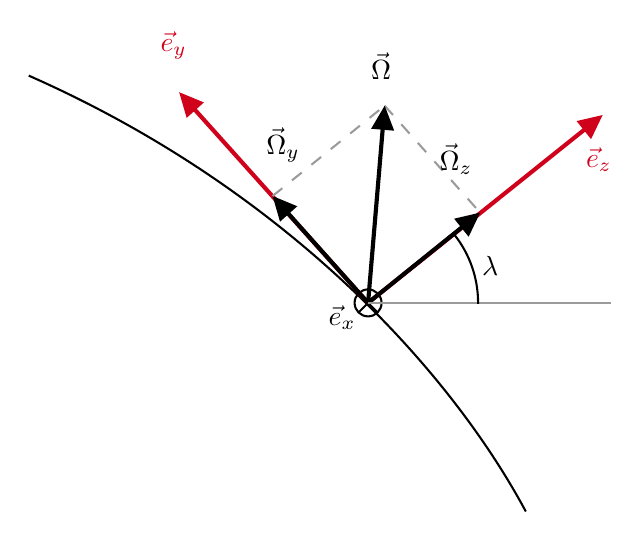
\begin{tikzpicture}[x=0.75pt,y=0.75pt,yscale=-1,xscale=1]
		%uncomment if require: \path (0,1215); %set diagram left start at 0, and has height of 1215
		
		%Curve Lines [id:da21077242529333717] 
		\draw    (163,96) .. controls (285.5,150) and (365.5,237) .. (402.5,306) ;
		%Flowchart: Summing Junction [id:dp36521170434362427] 
		\draw   (320,205.5) .. controls (320,201.91) and (322.91,199) .. (326.5,199) .. controls (330.09,199) and (333,201.91) .. (333,205.5) .. controls (333,209.09) and (330.09,212) .. (326.5,212) .. controls (322.91,212) and (320,209.09) .. (320,205.5) -- cycle ; \draw   (321.9,200.9) -- (331.1,210.1) ; \draw   (331.1,200.9) -- (321.9,210.1) ;
		%Straight Lines [id:da2821700767400266] 
		\draw [color={rgb, 255:red, 208; green, 2; blue, 27 }  ,draw opacity=1 ][line width=1.5]    (326.5,205.5) -- (238.17,106.98) ;
		\draw [shift={(235.5,104)}, rotate = 48.12] [fill={rgb, 255:red, 208; green, 2; blue, 27 }  ,fill opacity=1 ][line width=0.08]  [draw opacity=0] (11.61,-5.58) -- (0,0) -- (11.61,5.58) -- cycle    ;
		%Straight Lines [id:da11009230459230834] 
		\draw [color={rgb, 255:red, 208; green, 2; blue, 27 }  ,draw opacity=1 ][line width=1.5]    (326.5,205.5) -- (436.38,117.5) ;
		\draw [shift={(439.5,115)}, rotate = 141.31] [fill={rgb, 255:red, 208; green, 2; blue, 27 }  ,fill opacity=1 ][line width=0.08]  [draw opacity=0] (11.61,-5.58) -- (0,0) -- (11.61,5.58) -- cycle    ;
		%Straight Lines [id:da9256591158275844] 
		\draw [line width=1.5]    (326.5,205.5) -- (283.16,156.98) ;
		\draw [shift={(280.5,154)}, rotate = 48.23] [fill={rgb, 255:red, 0; green, 0; blue, 0 }  ][line width=0.08]  [draw opacity=0] (11.61,-5.58) -- (0,0) -- (11.61,5.58) -- cycle    ;
		%Straight Lines [id:da36515929878639275] 
		\draw [line width=1.5]    (326.5,205.5) -- (377.38,164.51) ;
		\draw [shift={(380.5,162)}, rotate = 141.15] [fill={rgb, 255:red, 0; green, 0; blue, 0 }  ][line width=0.08]  [draw opacity=0] (11.61,-5.58) -- (0,0) -- (11.61,5.58) -- cycle    ;
		%Straight Lines [id:da9447768138520616] 
		\draw [color={rgb, 255:red, 155; green, 155; blue, 155 }  ,draw opacity=1 ] [dash pattern={on 4.5pt off 4.5pt}]  (280.5,154) -- (334.5,110.5) ;
		%Straight Lines [id:da0825120567969524] 
		\draw [color={rgb, 255:red, 155; green, 155; blue, 155 }  ,draw opacity=1 ] [dash pattern={on 4.5pt off 4.5pt}]  (334.5,110.5) -- (380.5,162) ;
		%Straight Lines [id:da5394834769753507] 
		\draw [line width=1.5]    (326.5,205.5) -- (334.16,114.49) ;
		\draw [shift={(334.5,110.5)}, rotate = 94.81] [fill={rgb, 255:red, 0; green, 0; blue, 0 }  ][line width=0.08]  [draw opacity=0] (11.61,-5.58) -- (0,0) -- (11.61,5.58) -- cycle    ;
		%Straight Lines [id:da7391935837090116] 
		\draw [color={rgb, 255:red, 155; green, 155; blue, 155 }  ,draw opacity=1 ]   (326.5,205.5) -- (443.5,205.5) ;
		%Shape: Arc [id:dp37593752829137794] 
		\draw  [draw opacity=0] (368.25,172.85) .. controls (375.3,181.85) and (379.5,193.18) .. (379.5,205.5) .. controls (379.5,205.66) and (379.5,205.83) .. (379.5,205.99) -- (326.5,205.5) -- cycle ; \draw   (368.25,172.85) .. controls (375.3,181.85) and (379.5,193.18) .. (379.5,205.5) .. controls (379.5,205.66) and (379.5,205.83) .. (379.5,205.99) ;  
		
		% Text Node
		\draw (306,205.4) node [anchor=north west][inner sep=0.75pt]    {$\vec{e}_{x}$};
		% Text Node
		\draw (225,73.4) node [anchor=north west][inner sep=0.75pt]  [color={rgb, 255:red, 208; green, 2; blue, 27 }  ,opacity=1 ]  {$\vec{e}_{y}$};
		% Text Node
		\draw (430,129.4) node [anchor=north west][inner sep=0.75pt]  [color={rgb, 255:red, 208; green, 2; blue, 27 }  ,opacity=1 ]  {$\vec{e}_{z}$};
		% Text Node
		\draw (276,119.4) node [anchor=north west][inner sep=0.75pt]    {$\vec{\Omega }_{y}$};
		% Text Node
		\draw (359.5,127.4) node [anchor=north west][inner sep=0.75pt]    {$\vec{\Omega }_{z}$};
		% Text Node
		\draw (326.5,83.4) node [anchor=north west][inner sep=0.75pt]    {$\vec{\Omega }$};
		% Text Node
		\draw (380,181.4) node [anchor=north west][inner sep=0.75pt]    {$\lambda $};
		
		\end{tikzpicture}	 
		\vspace*{3mm}
		\caption[]{Reference frame linked to the cyclone with the planar pulse}
	\end{figure}
	Therefore:
	
	Hence we have:
	
	As we study the movements (almost) horizontal in the atmosphere at this latitude, we can consider that the fluid particles are liable to remain in the horizontal plane $(\vec{e}_x,\vec{e}_y)$. The components of the Coriolis force in a planar motion are therefore ($v_z=0$):
	
	where $f$ is named the "\NewTerm{Coriolis parameter}\index{Coriolis parameter}". So the Coriolis force in oceanography and meteorology is traditionally denoted:
	
	The number $f$, positive in the northern hemisphere, negative in the southern hemisphere, ranging from $0$ to $1.458$ at the poles while the force is of the order of thousandths of Newton for fluid masses (ocean currents) and of the same magnitude (because the speed compensates for the low density) for gas (air currents).
	
	We now apply the approximation of the geostrophic equilibrium, that is to say that we consider that the air is animated by a uniform rectilinear motion (geostrophic wind), in other words, we neglect the action of centrifugal force due to the rotation of the vortex relatively that of the Coriolis force due to the rotation of the Earth, which means we assume that:
	
	with $R$ being the radius of the vortex and $\omega$ its pulsation. Since (\SeeChapter{see section Classical Mechanics page \pageref{kinematics of circular motion}}):
	
	the latter inequality becomes:
	
	where:
	
	is named the "\NewTerm{Rossby number}\index{Rossby number}" and has no dimensions. A small Rossby number signifies a system which is strongly affected by Coriolis forces, and a large Rossby number signifies a system in which inertial and centrifugal forces dominate. For example, in tornadoes, the Rossby number is large ($\cong 10^3$), in low-pressure systems it is low ($\cong 0.1-1$) and in oceanic systems it is of the order of unity, but depending on the phenomena can range over several orders of magnitude ($\cong 10^{-2}-10^2$). As a result, in tornadoes the Coriolis force is negligible, and balance is between pressure and centrifugal forces (named "\NewTerm{cyclostrophic balance}\index{cyclostrophic balance}"). 
	\begin{tcolorbox}[title=Remark,arc=10pt,breakable,drop lifted shadow,
  skin=enhanced,
  skin first is subskin of={enhancedfirst}{arc=10pt,no shadow},
  skin middle is subskin of={enhancedmiddle}{arc=10pt,no shadow},
  skin last is subskin of={enhancedlast}{drop lifted shadow}]
	For the middle latitudes ($\lambda=45^\circ$), the experiences and measures give $f=10^{-4}\;[\text{m}\cdot\text{s}^{-1}]$ and $v=10\;[\text{m}\cdot \text{s}^{-1}]$. The limit value for which $R_0=1$ is $R=100\;[\text{km}]$. For a larger scale, that is the case with hurricanes where $R\cong 100\;[\text{km}]$ we are close to the geostrophic balance. For a smaller scale, the Coriolis force is negligible and the wind is accelerated from high to low pressure.
	\end{tcolorbox}
	In other words the Rossby number therefore represents the ratio between the forces of inertia and the forces due to rotation that characterize the motion of a fluid in a rotating frame.

	So we can make the difference between a geophysical flow with a large Rossby number or with a small Rossby number. If the Rossby number is greater than one, then the Coriolis forces due for example to Earth's rotation are negligible relatively to the flow inertia. Otherwise for a Rossby number very smaller than the unit, the Coriolis forces dominate the movement of the fluid.

	Thus, if one approaches the equator, $f$ tends to $0$ the Rossby number becomes very large and at the poles it becomes very weak respectively.

	Under this approximation, our Euler equation can be written as:
	
	and since we are interested only to the horizontal plane of the atmosphere this simplifies even more to the form:
	
	Thus in fully developed vector form by taking back the capital $P$ for pressure as it is customary in meteorology:
	
	It comes then:
	
	Therefore in conventional form:
	
	The norm being given by:
	
	Therefore:
	
	which is named the "\NewTerm{equation of geostrophic winds}\index{equation of geostrophic winds}".
	
	Four scenarios are to be considered (with some reminders about some concepts already introduced at the beginning of the section):
	\begin{enumerate}
		\item We are in the northern hemisphere and therefore $f$ is positive. Let us suppose that $\mathrm{d}P / \mathrm{d}R$ is positive, then the pressure increases away from the vortex center (which latter is therefore a minimum of low pressure). Therefore $v$ is positive and we have a vortex named "depression" in the northern hemisphere. Thus, the fluid (the wind) blows around the depression counter-clockwise (West direction) in the Northern Hemisphere.

		\textbf{Definitions (\#\thesection.\mydef):} 
		\begin{enumerate}
			\item[D1.] A "\NewTerm{depression}\index{depression}" (or "low pressure") is an area where the atmospheric pressure decreases horizontally toward a center of low pressure, that is to say a local minimum pressure.
	
			\item[D2.] The intense weather systems circulating around a closed center of low pressure (like a vacuum that attracts clouds from which the fact such systems are visible on satellite photos) consistently receive in  general the term "\NewTerm{cyclone}\index{cyclone}" or "\NewTerm{tropical cyclone}\index{tropical cyclone}".
		\end{enumerate}
		\begin{figure}[H]
			\begin{center}
				\includegraphics[scale=0.8]{img/engineering/cyclones.jpg}
			\end{center}	
			\caption[]{Some northern hemisphere cyclones}
		\end{figure}
		\begin{tcolorbox}[title=Remark,arc=10pt,breakable,drop lifted shadow,
  skin=enhanced,
  skin first is subskin of={enhancedfirst}{arc=10pt,no shadow},
  skin middle is subskin of={enhancedmiddle}{arc=10pt,no shadow},
  skin last is subskin of={enhancedlast}{drop lifted shadow}]
		On Earth we frequently associate depressions to bad weather because the dynamics surrounding depression presupposes the existence of updrafts (can hardly get into the ground so the only way to escape is up!) that cause clouds and precipitation. In addition, the pressure gradient over a depression can cause strong winds.
		\end{tcolorbox}
	
		\item We are still in the Northern Hemisphere and therefore $f$ is positive. Let us suppose that $\mathrm{d}P / \mathrm{d}R$ is negative this time, the pressure then decreases away from the vortex center (which is thus reaching a maximum pressure). Therefore $v$ is negative and we have a vortex named a "\NewTerm{high pressure}\index{high pressure}" in the northern hemisphere. Thus, the fluid (wind) blows around the high pressure clockwise (to the East) in the Northern Hemisphere.

		\textbf{Definitions (\#\thesection.\mydef):} 
		\begin{enumerate}
			\item[D1.] A "\NewTerm{high pressure}\index{high pressure}" is an area where the atmospheric pressure increases horizontally toward a center of high pressure, that is to say a local maximum pressure.
	
			\item[D2.] The intense weather systems to flow around a closed center of high pressure (as a fan it rejects and disperses the clouds from which the fact that the high pressure are not simply visible on satellite photos) consistently receive the name of "\NewTerm{anticyclone}\index{anticyclone}".
		\end{enumerate}
		\begin{tcolorbox}[title=Remark,arc=10pt,breakable,drop lifted shadow,
  skin=enhanced,
  skin first is subskin of={enhancedfirst}{arc=10pt,no shadow},
  skin middle is subskin of={enhancedmiddle}{arc=10pt,no shadow},
  skin last is subskin of={enhancedlast}{drop lifted shadow}]
		Anticyclones usually bring good weather and clear skies. Atmospheric dynamics causes air at medium altitudes to be relatively warm and dry, and therefore without clouds.
		\end{tcolorbox}

		\item We are still in the southern hemisphere and therefore $f$ is negative. Let us suppose $\mathrm{d}P /\mathrm{d}R$ is positive, then the pressure increases away from the vortex center. Therefore $v$ is negative and we have a vortex still named a "high pressure" (or "anticyclone") in the Southern Hemisphere. Thus, the fluid (wind) blows around the high pressure but counter-clockwise (to the West) in the Southern Hemisphere.

		\item We are still in the southern hemisphere and therefore $f$ is negative. Let us suppose that $\mathrm{d}P/\mathrm{d}R$ is negative, the pressure decreases away from the vortex center. Therefore $v$ is positive and we have a vortex still named "low pressure" (or "Hurricane") in the Southern Hemisphere. Thus, the fluid (the wind) blows around the low pressure clockwise (to the East) in the Southern Hemisphere.
	\end{enumerate}
	\begin{tcolorbox}[title=Remark,arc=10pt,breakable,drop lifted shadow,
  skin=enhanced,
  skin first is subskin of={enhancedfirst}{arc=10pt,no shadow},
  skin middle is subskin of={enhancedmiddle}{arc=10pt,no shadow},
  skin last is subskin of={enhancedlast}{drop lifted shadow}]
	It is therefore possible to say generally on larger dimensions that the wind comes from high pressure (anticyclone) to move towards low pressure (depression).
	\end{tcolorbox}
	Here is an illustration example of a depression (anticyclone) and high pressure (cyclone) in the Northern Hemisphere such as represented by professional practitioners of meteorology:
	\begin{figure}[H]
		\centering
		\includegraphics[scale=1]{img/engineering/low_high_pressure.jpg}	
		\caption{Low pressure and high pressure illustration}
	\end{figure}
	We can indeed observe that depression (D) rotates counter-clockwise and the high pressure (A) clockwise (and vice versa in the southern hemisphere).
	
	
	\pagebreak
	\subsection{Tides}
	Tides are the rise and fall of sea levels (but also from Earth's atmosphere layers\footnote{At the opposite of sea tides where the Moon has the main influence, for the atmosphere it is the Sun (because that latter is strongly heating the atmosphere layers too!)}!) caused by the combined effects of the gravitational forces exerted by the Moon and the Sun and the rotation of the Earth. The times and amplitude of tides at a locale are influenced by the alignment of the Sun and Moon, by the pattern of tides in the deep ocean, by the amphidromic systems of the oceans, and the shape of the coastline and near-shore bathymetry. Tides vary on timescales ranging from hours to years due to a number of factors.

	Tidal phenomena are not limited to the oceans, but can occur in other systems whenever a gravitational field that varies in time and space is present. For example, the solid part of the Earth is affected by tides (GPS measurements seems to give ground tides between $0$ to $28$ [cm] depending on the place on Earth and the composition of the ground), though this is not as easily seen as the water tidal movements.
	
	Among the phenomena of nature, the tide is one of the most majestic in its scope and power, one of the more surprising by its regularity and the discretion of its causes. We can then easily understand not only that it is imposed to the attention of the traveller but it has, since the remotest antiquity, aroused the research of the most distinguished scholars.

	To approach the subject of tides in a simply way, we can state from a simple vectorial analysis that: If the Lunar attraction was identical at each point of the Earth, there would be no tides. We must therefore approach the study of tides on the differences of forces. The influence of the Moon on the tides is named the "\NewTerm{diurnal component}\index{diurnal component}" and should explain why there are tides twice a day\footnote{Even if most tides are visible by the human eyes on beaches of Ocean and Seas, for lakes tides also exist but are difficult to observe. We need careful experimental measurements as the amplitudes are very small and take into account that most of the time for lakes the weather (atmospheric pressure) has more impact than the Moon itself...}.
	\begin{figure}[H]
		\centering
		\includegraphics[scale=0.74]{img/engineering/mont_saint_michel_tides.jpg}
		\caption{High and low tide at Mont Saint-Michel in France}
	\end{figure}
	Another nice phenomenon to study mathematically (and to see in real life or on YouTube) are the "tidal bore" which is the leading edge of the incoming tide that forms a wave (or waves) of water that travels up a river or narrow bay against the direction of the river or bay's current\footnote{The world largest tidal bore at the time we write these lines seems to be the one located in China's Zhejiang province where it can reach a maximum of nine meter in height at a speed of $40\;[\text{km}\cdot\text{h}^{-1}]$}:
	\begin{figure}[H]
		\centering
		\includegraphics[scale=0.55]{img/engineering/tidal_bore.jpg}
		\caption{Tidal bore}
	\end{figure}
	The most common type of tides are (some have cyclic and others are totally random and their duration vary a lot):
	\begin{itemize}
		\item Astronomical tides (influence Moon/Sun)
		\item Rotational tides (due to rotation of Earth)
		\item Atmospheric tides/Barometric tides\footnote{In areas of high pressure (anticyclones), the sea level decreases. Inversely in areas of low pressure (cyclones). Mean sea level (level 0) corresponds to a pressure of $1013.25$ hectopascals (reference pressure). It is necessary to add $1$ [cm] or remove $1$ [cm] of water height per hectopascal of difference with the reference pressure.} (due to meteorological conditions)
		\item Wind tides\footnote{A strong and constant offshore wind causes a drop in sea level of up to 1 meter. Conversely in case of opposite wind direction.} (due to the effect of winds on large sea areas)
		\item Tectonic tides (due to earthquakes)
	\end{itemize}
	The ocean and seas tides on Earth are caused by both the Moon's gravity and the Sun's gravity. In general, ocean and seas tides are not generated by the overall strength of gravity as we will see it, but instead by the differences in gravity from one spot to the next (the gravitational gradient). Even though the Sun is much more massive and therefore has stronger overall gravity than the Moon, the Moon is closer to the Earth so that its gravitational gradient is stronger than that of the Sun. Because ocean and seas tides are the effect of ocean water responding to a gravitational gradient, the Moon plays a larger role in creating tides than does the Sun. But the Sun's gravitational gradient across the Earth is significant and it does contribute to tides as well.
	
	As the tides are caused by the gradient of the gravitational field, the tidal force experienced drops with the third power of the distance. This means that the relative strength of the tides should go as :
	
	So although the Sun is more massive, its greater distance makes its tidal force about $2.3\times$ weaker than the Moon.
	
	\subsubsection{Astronomical tides}
	Let us first deal with the most famous type of tide that are the astronomical one (due mainly to Sun and Moon)!
	
	\paragraph{First approach}\mbox{}\\\\
	Let us consider for the naive study of tilde a mass of water $m$ at the equator and at the poles of a rigid Earth (i.e. ground not under the influence of the Moon gravity). We will calculate the attractive force on the mass relatively to the center of the Earth and taking into account the influence of the Moon that has a mass $M_L$ (Lunar influence).
	\begin{figure}[H]
		\centering
		% Gradient Info
		  
		\tikzset {_ct5opcmz6/.code = {\pgfsetadditionalshadetransform{ \pgftransformshift{\pgfpoint{0 bp } { 0 bp }  }  \pgftransformscale{1 }  }}}
		\pgfdeclareradialshading{_werelompm}{\pgfpoint{0bp}{0bp}}{rgb(0bp)=(0.92,0.95,0.97);
		rgb(0.08117079734802246bp)=(0.92,0.95,0.97);
		rgb(25bp)=(0.77,0.88,0.95);
		rgb(400bp)=(0.77,0.88,0.95)}
		
		% Gradient Info
		  
		\tikzset {_dzrpe9j5z/.code = {\pgfsetadditionalshadetransform{ \pgftransformshift{\pgfpoint{-75 bp } { 286.5 bp }  }  \pgftransformscale{1 }  }}}
		\pgfdeclareradialshading{_htsly8mvi}{\pgfpoint{80bp}{-304bp}}{rgb(0bp)=(1,1,1);
		rgb(0bp)=(1,1,1);
		rgb(25bp)=(0.5,0.5,0.5);
		rgb(400bp)=(0.5,0.5,0.5)}
		
		% Gradient Info
		  
		\tikzset {_3mzzaev32/.code = {\pgfsetadditionalshadetransform{ \pgftransformshift{\pgfpoint{0 bp } { 0 bp }  }  \pgftransformrotate{0 }  \pgftransformscale{2 }  }}}
		\pgfdeclarehorizontalshading{_oqr370t9z}{150bp}{rgb(0bp)=(0.5,0.5,0.5);
		rgb(37.5811653477805bp)=(0.5,0.5,0.5);
		rgb(62.49188508306231bp)=(0.61,0.61,0.61);
		rgb(100bp)=(0.61,0.61,0.61)}
		\tikzset{every picture/.style={line width=0.75pt}} %set default line width to 0.75pt        
		
		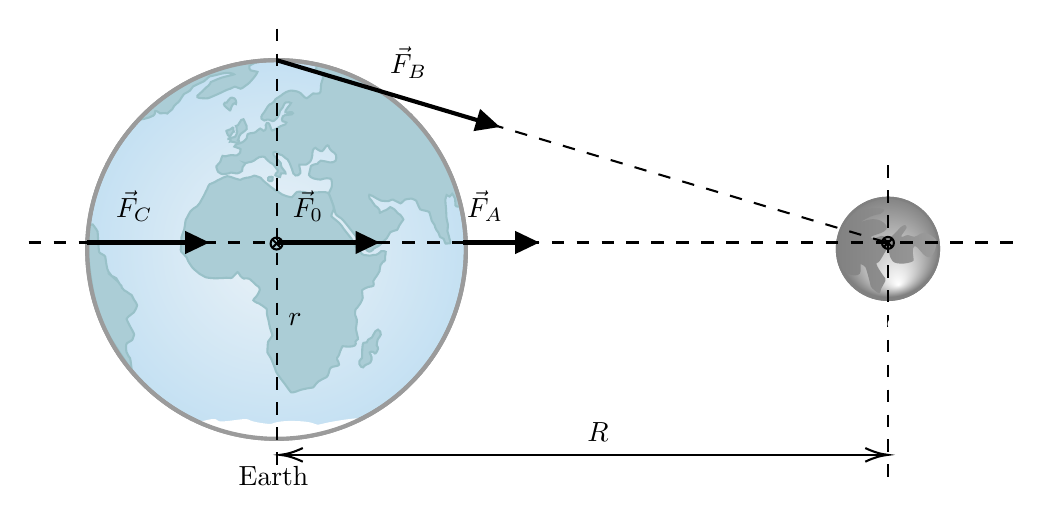
\begin{tikzpicture}[x=0.75pt,y=0.75pt,yscale=-1,xscale=1]
		%uncomment if require: \path (0,518); %set diagram left start at 0, and has height of 518
		
		%Shape: Circle [id:dp8938982774548756] 
		\path  [shading=_werelompm,_ct5opcmz6] (114.55,158.96) .. controls (114.55,108.58) and (155.39,67.73) .. (205.78,67.73) .. controls (256.16,67.73) and (297,108.58) .. (297,158.96) .. controls (297,209.34) and (256.16,250.18) .. (205.78,250.18) .. controls (155.39,250.18) and (114.55,209.34) .. (114.55,158.96) -- cycle ; % for fading 
		 \draw  [color={rgb, 255:red, 155; green, 155; blue, 155 }  ,draw opacity=1 ][line width=1.5]  (114.55,158.96) .. controls (114.55,108.58) and (155.39,67.73) .. (205.78,67.73) .. controls (256.16,67.73) and (297,108.58) .. (297,158.96) .. controls (297,209.34) and (256.16,250.18) .. (205.78,250.18) .. controls (155.39,250.18) and (114.55,209.34) .. (114.55,158.96) -- cycle ; % for border 
		
		%Shape: Polygon Curved [id:ds03522640822952505] 
		\draw  [color={rgb, 255:red, 153; green, 193; blue, 200 }  ,draw opacity=1 ][fill={rgb, 255:red, 171; green, 205; blue, 214 }  ,fill opacity=1 ] (247.27,204.94) .. controls (247.63,202.89) and (248.48,204.46) .. (249.2,203.73) .. controls (249.93,203.01) and (249.27,203.03) .. (249.93,202.4) .. controls (250.59,201.78) and (251.02,201.88) .. (251.75,201.31) .. controls (252.49,200.73) and (252.24,199.92) .. (252.72,199.49) .. controls (253.2,199.07) and (253.56,197.33) .. (254.66,197.56) .. controls (255.75,197.79) and (256.02,199.16) .. (255.99,199.98) .. controls (255.95,200.79) and (254.98,201.22) .. (254.53,202.27) .. controls (254.09,203.32) and (254.06,204.87) .. (254.04,205.19) .. controls (254.02,205.5) and (255.38,206.14) .. (254.17,208.08) .. controls (252.96,210.01) and (253.08,208.63) .. (252.36,208.32) .. controls (251.64,208.01) and (250.96,208.12) .. (250.67,208.56) .. controls (250.37,209) and (252,210.13) .. (251.51,212.19) .. controls (251.03,214.24) and (249.86,213.75) .. (248.61,214.6) .. controls (247.36,215.45) and (247.38,216.56) .. (246.54,215.46) .. controls (245.71,214.36) and (245.34,213.95) .. (245.71,212.79) .. controls (246.08,211.63) and (246.77,211.86) .. (246.92,211.34) .. controls (247.07,210.82) and (246.91,207) .. (247.27,204.94) -- cycle ;
		%Shape: Polygon Curved [id:ds5157320992246872] 
		\draw  [color={rgb, 255:red, 153; green, 193; blue, 200 }  ,draw opacity=1 ][fill={rgb, 255:red, 171; green, 205; blue, 214 }  ,fill opacity=1 ] (183.56,85.98) .. controls (184.42,85.42) and (186.46,86.18) .. (186.34,88.11) .. controls (186.22,90.04) and (185.93,87.6) .. (184.76,89) .. controls (183.6,90.4) and (183.68,92.58) .. (183.19,91.9) .. controls (182.71,91.22) and (180.56,90.24) .. (180.41,88.96) .. controls (180.26,87.67) and (181.36,88.61) .. (181.74,88.23) .. controls (182.12,87.86) and (182.69,86.53) .. (183.56,85.98) -- cycle ;
		%Shape: Polygon Curved [id:ds1955429013119243] 
		\draw  [color={rgb, 255:red, 153; green, 193; blue, 200 }  ,draw opacity=1 ][fill={rgb, 255:red, 171; green, 205; blue, 214 }  ,fill opacity=1 ] (203.25,123.91) .. controls (204.12,123.35) and (203.98,124.63) .. (203.86,125.48) .. controls (203.73,126.33) and (203.13,125.96) .. (202.4,125.96) .. controls (201.68,125.96) and (201.56,125.48) .. (201.68,124.51) .. controls (201.8,123.54) and (202.39,124.46) .. (203.25,123.91) -- cycle ;
		%Shape: Polygon Curved [id:ds4612751901702774] 
		\draw  [color={rgb, 255:red, 153; green, 193; blue, 200 }  ,draw opacity=1 ][fill={rgb, 255:red, 171; green, 205; blue, 214 }  ,fill opacity=1 ] (165.77,77.13) .. controls (169.52,75.44) and (183.97,70.47) .. (186.87,69.87) .. controls (189.78,69.26) and (190.68,68.95) .. (192.97,68.67) .. controls (195.27,68.38) and (198.9,68.28) .. (197.57,68.43) .. controls (196.23,68.57) and (193.33,69.81) .. (192.73,70.48) .. controls (192.13,71.15) and (193.01,72.49) .. (193.34,72.66) .. controls (193.67,72.82) and (196.45,73.27) .. (196.6,73.38) .. controls (196.76,73.5) and (195.46,75.39) .. (195.03,75.92) .. controls (194.6,76.45) and (192.67,78.77) .. (192.01,79.19) .. controls (191.34,79.6) and (189,81.57) .. (188.5,81.48) .. controls (188,81.39) and (186.11,80.57) .. (185.72,80.52) .. controls (185.33,80.46) and (183.44,81.69) .. (182.82,81.72) .. controls (182.2,81.75) and (179.42,83.23) .. (178.93,83.44) .. controls (178.44,83.64) and (173.23,86.06) .. (172.64,86.1) .. controls (172.05,86.14) and (167.87,86.19) .. (167.65,85.58) .. controls (167.43,84.98) and (167.52,84.82) .. (168.74,83.89) .. controls (169.96,82.96) and (171.53,80.9) .. (172.85,80.14) .. controls (174.17,79.39) and (173.54,78.56) .. (174.06,78.33) .. controls (174.58,78.09) and (176.4,77.32) .. (177.6,76.79) .. controls (178.79,76.26) and (179.94,75.99) .. (181.47,75.58) .. controls (183,75.17) and (185.05,74.72) .. (185.3,74.58) .. controls (185.56,74.44) and (183.32,73.85) .. (182.88,73.85) .. controls (182.45,73.86) and (180.23,73.85) .. (178.29,74.46) .. controls (176.36,75.06) and (173.82,75.48) .. (173.58,75.55) .. controls (173.33,75.62) and (171.06,77.79) .. (170.67,77.97) .. controls (170.29,78.14) and (165.66,80.3) .. (165.6,80.38) .. controls (165.53,80.46) and (164.5,81.85) .. (164.02,82.44) .. controls (163.55,83.03) and (161.78,83.55) .. (161.24,84.01) .. controls (160.7,84.47) and (159.07,87.52) .. (158.46,88) .. controls (157.86,88.48) and (157.15,88.94) .. (156.53,89.69) .. controls (155.9,90.45) and (155.62,91.31) .. (155.56,91.39) .. controls (155.5,91.46) and (153.15,93.31) .. (153.14,93.44) .. controls (153.14,93.57) and (151.4,92.75) .. (150.48,93.32) .. controls (149.57,93.89) and (149.69,93.03) .. (148.07,92.35) .. controls (146.44,91.67) and (147.87,93.56) .. (146.49,94.41) .. controls (145.12,95.25) and (143.6,95.6) .. (142.14,95.98) .. controls (140.69,96.36) and (140.13,96.35) .. (140.09,95.97) .. controls (140.04,95.59) and (149.33,87.14) .. (150.36,86.66) .. controls (151.4,86.18) and (162.02,78.82) .. (165.77,77.13) -- cycle ;
		%Shape: Polygon Curved [id:ds3657837033917619] 
		\draw  [color={rgb, 255:red, 153; green, 193; blue, 200 }  ,draw opacity=1 ][fill={rgb, 255:red, 171; green, 205; blue, 214 }  ,fill opacity=1 ] (186.81,102.13) .. controls (186.73,101.27) and (186.33,101.89) .. (186.57,100.68) .. controls (186.81,99.47) and (185.87,99.69) .. (186.2,99.47) .. controls (186.54,99.26) and (187.9,99.11) .. (187.9,97.91) .. controls (187.9,96.7) and (189.47,96.18) .. (189.83,96.21) .. controls (190.2,96.24) and (190.28,97.57) .. (190.8,98.27) .. controls (191.31,98.97) and (191.67,100.12) .. (191.4,100.93) .. controls (191.13,101.73) and (189.96,101.88) .. (189.59,102.5) .. controls (189.22,103.11) and (187.95,103.07) .. (187.78,104.43) .. controls (187.6,105.79) and (187.25,106.01) .. (187.17,106.25) .. controls (187.09,106.48) and (188.02,106.12) .. (187.78,106.97) .. controls (187.7,107.24) and (187.52,107.4) .. (187.26,107.48) .. controls (186.71,107.64) and (185.78,107.42) .. (184.63,107.09) .. controls (182.94,106.61) and (183.16,107.68) .. (183.67,106.25) .. controls (184.17,104.81) and (182.02,106.12) .. (182.58,105.52) .. controls (183.14,104.92) and (185.76,105.24) .. (186.08,104.31) .. controls (186.41,103.38) and (186.88,103) .. (186.81,102.13) -- cycle ;
		%Shape: Polygon Curved [id:ds2972959762730816] 
		\draw  [color={rgb, 255:red, 153; green, 193; blue, 200 }  ,draw opacity=1 ][fill={rgb, 255:red, 171; green, 205; blue, 214 }  ,fill opacity=1 ] (183.54,101.05) .. controls (184.41,100.49) and (185.12,99.35) .. (185,101.29) .. controls (184.87,103.22) and (185.81,101.15) .. (184.64,102.54) .. controls (183.48,103.94) and (183.42,104.99) .. (182.94,104.31) .. controls (182.46,103.63) and (182.12,104.27) .. (181.97,102.98) .. controls (181.82,101.69) and (181.24,102.15) .. (181.62,101.77) .. controls (182,101.4) and (182.68,101.6) .. (183.54,101.05) -- cycle ;
		%Shape: Polygon Curved [id:ds30547861733844095] 
		\draw  [color={rgb, 255:red, 153; green, 193; blue, 200 }  ,draw opacity=1 ][fill={rgb, 255:red, 171; green, 205; blue, 214 }  ,fill opacity=1 ] (115.04,161.38) .. controls (114.91,159.48) and (115.04,147.6) .. (116.12,147) .. controls (117.21,146.39) and (117.26,147.03) .. (117.94,147.85) .. controls (118.62,148.66) and (119.33,149.85) .. (119.51,150.26) .. controls (119.69,150.67) and (119.99,159.57) .. (120.36,160.3) .. controls (120.72,161.02) and (123.02,161.51) .. (123.26,162.47) .. controls (123.5,163.44) and (123.86,168.52) .. (124.83,169.73) .. controls (125.8,170.94) and (126.47,171.79) .. (126.52,171.9) .. controls (126.57,172.02) and (125.86,171.38) .. (127.13,172.03) .. controls (128.39,172.67) and (128.94,172.75) .. (129.3,174.08) .. controls (129.66,175.41) and (130.94,176.21) .. (130.99,176.38) .. controls (131.05,176.55) and (131.24,178.23) .. (132.45,178.68) .. controls (133.65,179.12) and (135.35,180.81) .. (135.71,180.73) .. controls (136.07,180.65) and (136.51,182.39) .. (137.16,183.27) .. controls (137.81,184.15) and (138.49,185.08) .. (138.61,185.81) .. controls (138.73,186.53) and (137.77,187.82) .. (137.64,188.23) .. controls (137.52,188.64) and (136.64,190) .. (135.71,190.28) .. controls (134.78,190.56) and (133.59,192.23) .. (133.53,192.46) .. controls (133.48,192.69) and (135.3,196.19) .. (135.59,196.69) .. controls (135.88,197.19) and (137.35,199.74) .. (137.16,200.06) .. controls (136.97,200.39) and (136.42,202.45) .. (136.19,202.6) .. controls (135.97,202.75) and (134.55,203.57) .. (133.78,204.05) .. controls (133,204.54) and (133.29,206.71) .. (133.41,208.16) .. controls (133.53,209.61) and (134.98,210.58) .. (135.23,211.43) .. controls (135.47,212.27) and (136.06,217.16) .. (135.95,217.11) .. controls (135.84,217.06) and (125.31,201.39) .. (123.86,198.49) .. controls (122.41,195.59) and (119.11,187.54) .. (117.57,179.87) .. controls (116.04,172.21) and (115.17,163.27) .. (115.04,161.38) -- cycle ;
		%Shape: Polygon Curved [id:ds8162582902550839] 
		\draw  [color={rgb, 255:red, 153; green, 193; blue, 200 }  ,draw opacity=1 ][fill={rgb, 255:red, 171; green, 205; blue, 214 }  ,fill opacity=1 ] (230.97,132.19) .. controls (230.77,131.52) and (232.11,130.02) .. (232.3,129.05) .. controls (232.49,128.08) and (232.73,125.24) .. (231.7,124.82) .. controls (230.66,124.4) and (229.33,124.65) .. (228.37,124.89) .. controls (227.4,125.12) and (226.67,125.61) .. (225.46,125.13) .. controls (224.25,124.64) and (222.8,124.89) .. (222.2,124.04) .. controls (221.59,123.19) and (220.92,122.95) .. (221.59,121.98) .. controls (222.27,121.02) and (221.69,119.7) .. (222.3,118.85) .. controls (222.9,118.01) and (225.38,117.69) .. (225.56,117.64) .. controls (225.74,117.6) and (226.17,116.31) .. (227.13,116.19) .. controls (228.1,116.07) and (227.93,116.17) .. (229.38,116.53) .. controls (230.83,116.9) and (231.92,117.26) .. (233.12,116.9) .. controls (234.33,116.53) and (234.33,116.05) .. (234.58,114.84) .. controls (234.82,113.63) and (234.2,112.95) .. (233.54,112.32) .. controls (232.88,111.7) and (232.76,112.18) .. (231.55,110.61) .. controls (230.34,109.04) and (231.31,108.67) .. (230.34,108.79) .. controls (229.38,108.92) and (228.59,111.26) .. (227.68,111.58) .. controls (226.78,111.9) and (224.63,110.07) .. (224.54,110) .. controls (224.45,109.94) and (223.09,110.37) .. (223.09,112.18) .. controls (223.09,113.99) and (222.58,115.79) .. (222.12,116.41) .. controls (221.67,117.03) and (220.64,117.68) .. (220.19,117.98) .. controls (219.74,118.28) and (217.27,117.99) .. (216.8,118.1) .. controls (216.34,118.22) and (217.53,121.13) .. (217.23,122.09) .. controls (216.93,123.06) and (215.81,123.53) .. (214.93,123.3) .. controls (214.06,123.08) and (213.42,121.57) .. (213.48,121.13) .. controls (213.55,120.68) and (212.78,119.41) .. (212.66,118.81) .. controls (212.54,118.2) and (212.3,117.48) .. (211.93,116.99) .. controls (211.57,116.51) and (211.17,115.73) .. (211.09,115.54) .. controls (211.01,115.35) and (210.12,115.27) .. (209.39,114.33) .. controls (208.67,113.4) and (208.18,113.44) .. (207.22,113.13) .. controls (206.26,112.81) and (205.76,111.75) .. (205.04,111.92) .. controls (204.33,112.08) and (203.89,112.21) .. (204.32,113.25) .. controls (204.74,114.29) and (205.77,114.94) .. (206.13,115.54) .. controls (206.49,116.15) and (208.25,117.12) .. (207.89,118.2) .. controls (207.53,119.29) and (210.82,121.97) .. (210.1,122.34) .. controls (209.37,122.7) and (208.35,121.75) .. (207.92,122.34) .. controls (207.5,122.92) and (207.81,123.92) .. (207.44,124.03) .. controls (207.06,124.14) and (205.35,123.76) .. (205.16,123.14) .. controls (204.98,122.51) and (205.79,122.16) .. (206.2,121.71) .. controls (206.6,121.26) and (206.32,120.38) .. (205.59,119.77) .. controls (204.87,119.17) and (205.1,119.32) .. (204.38,118.2) .. controls (203.66,117.09) and (203.18,117.66) .. (202.57,116.99) .. controls (201.96,116.33) and (201.27,115.82) .. (200.55,115.05) .. controls (199.82,114.28) and (200.47,114.4) .. (199.1,114.2) .. controls (197.72,114.01) and (196.87,114.79) .. (196.07,115.29) .. controls (195.28,115.79) and (194.26,116.74) .. (193.54,116.74) .. controls (192.81,116.74) and (190.02,117.64) .. (190.63,117.35) .. controls (191.25,117.05) and (189.89,118.71) .. (189.42,119.28) .. controls (188.96,119.85) and (189.62,120.49) .. (189.18,121.09) .. controls (188.74,121.7) and (187.28,122.18) .. (186.89,122.3) .. controls (186.49,122.43) and (183.48,121.68) .. (183.49,121.99) .. controls (183.5,122.31) and (180.47,122.58) .. (179.87,122.67) .. controls (179.27,122.75) and (177.55,121.55) .. (177.57,121.51) .. controls (177.58,121.47) and (176.49,119.28) .. (176.85,118.8) .. controls (177.21,118.31) and (178.55,116.92) .. (178.66,116.74) .. controls (178.78,116.57) and (179.51,113.89) .. (179.75,113.84) .. controls (179.99,113.79) and (180.83,114.17) .. (181.08,114.09) .. controls (181.33,114.01) and (182.78,113.67) .. (183.02,113.61) .. controls (183.26,113.55) and (184.38,113.41) .. (184.59,113.49) .. controls (184.8,113.57) and (186.41,113.7) .. (186.64,113.61) .. controls (186.88,113.52) and (188.22,112.44) .. (188.22,112.29) .. controls (188.22,112.14) and (188.46,110.8) .. (188.46,110.6) .. controls (188.45,110.39) and (185.53,109.48) .. (185.43,109.39) .. controls (185.34,109.3) and (186.36,108.17) .. (186.64,108.18) .. controls (186.93,108.19) and (188.16,107.67) .. (188.34,107.7) .. controls (188.51,107.72) and (190.13,106.86) .. (190.15,106.73) .. controls (190.17,106.59) and (191.36,105.57) .. (191.36,105.4) .. controls (191.36,105.22) and (191.79,103.63) .. (191.84,103.46) .. controls (191.9,103.3) and (193.61,102.65) .. (193.78,102.86) .. controls (193.94,103.07) and (195.6,102.61) .. (195.71,102.38) .. controls (195.82,102.14) and (197.68,100.78) .. (197.89,100.69) .. controls (198.09,100.61) and (199.27,101.65) .. (199.46,101.78) .. controls (199.65,101.91) and (200.96,101.22) .. (200.73,100.5) .. controls (200.51,99.78) and (200.37,98.44) .. (201.1,97.96) .. controls (201.82,97.47) and (202.79,99.05) .. (202.79,99.77) .. controls (202.79,100.5) and (203.5,101.6) .. (203.69,101.66) .. controls (203.88,101.72) and (205.11,100.93) .. (205.5,100.82) .. controls (205.9,100.7) and (207.78,99.35) .. (208.71,99.17) .. controls (209.65,98.98) and (210.63,98.47) .. (210.52,97.79) .. controls (210.41,97.11) and (209.4,97.75) .. (208.71,97.23) .. controls (208.03,96.72) and (208.35,96.02) .. (208.83,94.81) .. controls (209.32,93.61) and (213.85,94.51) .. (213.66,93.32) .. controls (213.47,92.13) and (210.85,93.39) .. (210.04,92.88) .. controls (209.24,92.37) and (212.97,88.67) .. (212.75,88.38) .. controls (212.52,88.1) and (211.18,87.78) .. (210.21,88.14) .. controls (209.24,88.51) and (209.01,90.67) .. (208.23,91.19) .. controls (207.45,91.7) and (207.38,92.28) .. (207.02,93.85) .. controls (206.66,95.42) and (205.25,96.38) .. (204.48,96.99) .. controls (203.71,97.6) and (201.95,95.88) .. (201.22,96.39) .. controls (200.48,96.89) and (199.32,97.15) .. (198.56,96.02) .. controls (197.8,94.89) and (199.82,92.88) .. (199.81,92.86) .. controls (199.81,92.84) and (200.92,91.1) .. (201.02,90.92) .. controls (201.12,90.75) and (202.18,88.77) .. (203.39,88.65) .. controls (204.6,88.53) and (204.45,87.23) .. (205.25,86.57) .. controls (206.05,85.91) and (207.97,84.96) .. (208.88,84.03) .. controls (209.78,83.11) and (210.97,82.98) .. (211.78,82.58) .. controls (212.59,82.18) and (214.98,82.67) .. (215.17,82.7) .. controls (215.35,82.74) and (217.48,83.29) .. (218.07,84.4) .. controls (218.65,85.5) and (220.19,86.09) .. (220.36,86.09) .. controls (220.54,86.09) and (223.23,83.79) .. (223.39,83.79) .. controls (223.55,83.79) and (225.64,84) .. (226.41,83.67) .. controls (227.18,83.34) and (226.97,82.42) .. (227.01,82.34) .. controls (227.05,82.26) and (227.23,79.32) .. (227.26,79.2) .. controls (227.28,79.07) and (228.1,76.66) .. (228.22,75.93) .. controls (228.34,75.21) and (227.45,73.68) .. (226.53,73.51) .. controls (225.61,73.35) and (224.86,72.61) .. (224.84,72.55) .. controls (224.81,72.48) and (225.1,70.06) .. (225.1,70.01) .. controls (225.1,69.96) and (249.64,74.01) .. (270.32,94.56) .. controls (290.99,115.11) and (294.74,138.12) .. (294.74,138.18) .. controls (294.74,138.24) and (291.96,138.66) .. (291.96,137.69) .. controls (291.96,136.72) and (291.84,135.51) .. (291.84,134.91) .. controls (291.84,134.3) and (290.55,132.18) .. (290.39,132.13) .. controls (290.23,132.08) and (289.51,133.4) .. (289.18,133.46) .. controls (288.84,133.51) and (287.77,132.66) .. (287.73,132.73) .. controls (287.69,132.8) and (287.16,134.64) .. (287.12,134.79) .. controls (287.09,134.94) and (287.18,137.05) .. (287.24,137.33) .. controls (287.3,137.61) and (287.5,139.77) .. (287.5,140.23) .. controls (287.49,140.68) and (287.62,142.91) .. (287.61,143.37) .. controls (287.6,143.84) and (288.17,146.03) .. (288.33,147) .. controls (288.49,147.97) and (288.04,149.61) .. (288.09,150.02) .. controls (288.14,150.43) and (288.99,152.89) .. (288.94,153.17) .. controls (288.88,153.44) and (289.98,155.73) .. (289.3,155.95) .. controls (288.62,156.16) and (287.49,156.01) .. (287.24,156.07) .. controls (286.99,156.12) and (286.53,154.27) .. (286.4,154.01) .. controls (286.27,153.75) and (285,153) .. (284.7,153.04) .. controls (284.41,153.09) and (283.86,150.55) .. (283.37,150.26) .. controls (282.89,149.98) and (281.99,148.06) .. (282.04,147.6) .. controls (282.1,147.15) and (280.8,145.69) .. (280.59,145.19) .. controls (280.39,144.68) and (279.59,141.47) .. (279.38,140.97) .. controls (279.18,140.46) and (275.46,140.01) .. (275.03,139.64) .. controls (274.6,139.27) and (273.26,135.82) .. (273.1,135.52) .. controls (272.94,135.23) and (271.02,134.46) .. (270.8,134.44) .. controls (270.58,134.41) and (267.87,134.78) .. (267.66,134.92) .. controls (267.44,135.06) and (265.75,136.88) .. (265.48,136.73) .. controls (265.21,136.59) and (262.11,135.11) .. (261.85,134.92) .. controls (261.6,134.73) and (259.88,135.62) .. (259.68,135.65) .. controls (259.47,135.67) and (256.43,135.58) .. (256.05,135.4) .. controls (255.67,135.23) and (253.06,133.9) .. (252.91,133.71) .. controls (252.75,133.52) and (250.66,132.5) .. (250.49,132.6) .. controls (250.32,132.71) and (250.24,133.45) .. (250.61,134.41) .. controls (250.98,135.38) and (251.75,134.81) .. (252.18,136.35) .. controls (252.61,137.89) and (253.71,137.99) .. (254.48,138.77) .. controls (255.25,139.54) and (255.87,140.5) .. (255.45,141.19) .. controls (255.02,141.87) and (257.27,140.18) .. (258.59,139.98) .. controls (259.91,139.77) and (260.16,137.86) .. (261.13,138.77) .. controls (262.09,139.67) and (262.22,139.01) .. (263.31,140.46) .. controls (264.39,141.91) and (264.97,142) .. (265.24,142.15) .. controls (265.51,142.3) and (266.96,144.32) .. (266.88,144.53) .. controls (266.8,144.73) and (265.57,146.28) .. (264.88,147.47) .. controls (264.19,148.67) and (264.22,149.42) .. (263.79,149.53) .. controls (263.36,149.63) and (260.79,150.38) .. (260.52,150.74) .. controls (260.25,151.1) and (258.9,153.69) .. (258.57,153.86) .. controls (258.25,154.03) and (255.75,156.69) .. (255.45,156.78) .. controls (255.15,156.87) and (254.72,157.75) .. (253.51,157.99) .. controls (252.3,158.23) and (252.32,159.05) .. (252.18,159.08) .. controls (252.04,159.11) and (250.75,160.8) .. (249.47,159.52) .. controls (248.19,158.24) and (238.34,144.89) .. (237.02,144.04) .. controls (235.69,143.2) and (234.07,142.27) .. (233.99,141.02) .. controls (233.91,139.77) and (231.17,132.87) .. (230.97,132.19) -- cycle ;
		%Shape: Polygon Curved [id:ds7615015936100842] 
		\draw  [color={rgb, 255:red, 153; green, 193; blue, 200 }  ,draw opacity=1 ][fill={rgb, 255:red, 171; green, 205; blue, 214 }  ,fill opacity=1 ] (230.97,132.19) .. controls (231.7,133.47) and (232.67,136.76) .. (233.11,137.76) .. controls (233.55,138.76) and (233.52,140.17) .. (232.83,140.82) .. controls (232.14,141.46) and (232.3,142.68) .. (232.19,142.95) .. controls (232.08,143.23) and (236.18,145.86) .. (237.15,147.55) .. controls (238.11,149.24) and (241.06,152.64) .. (241.69,153.52) .. controls (242.31,154.4) and (243.12,156.34) .. (243.62,157.26) .. controls (244.12,158.19) and (245.55,158.47) .. (245.92,159.68) .. controls (246.28,160.89) and (247.48,161.6) .. (247.97,161.62) .. controls (248.46,161.63) and (250.98,162.09) .. (251.24,161.86) .. controls (251.49,161.63) and (252.99,161.56) .. (253.78,161.5) .. controls (254.56,161.43) and (255.47,160.42) .. (256.19,159.8) .. controls (256.92,159.19) and (258.36,160.09) .. (258.38,160.1) .. controls (258.4,160.12) and (258.21,162.01) .. (258.13,162.1) .. controls (258.05,162.19) and (258.14,163.14) .. (258.04,164.08) .. controls (257.95,165.02) and (257.32,164.59) .. (257.28,164.64) .. controls (257.24,164.69) and (256.41,165.65) .. (255.86,166.5) .. controls (255.32,167.35) and (255.81,168.52) .. (255.38,169.4) .. controls (254.95,170.28) and (254.4,171.08) .. (253.93,171.82) .. controls (253.46,172.55) and (252.42,173.76) .. (252.37,174.25) .. controls (252.31,174.73) and (253.34,176.77) .. (251.52,176.77) .. controls (249.71,176.77) and (247.18,178.22) .. (247.05,178.59) .. controls (246.92,178.96) and (247.23,181.87) .. (247.29,182.21) .. controls (247.36,182.56) and (246.26,184.84) .. (246.08,184.99) .. controls (245.91,185.15) and (244.64,187.29) .. (244.15,187.41) .. controls (243.66,187.54) and (243.22,190.45) .. (244.03,191.52) .. controls (244.84,192.59) and (244.27,195.75) .. (244.03,196.6) .. controls (243.79,197.45) and (245.29,202.01) .. (244.99,202.14) .. controls (244.7,202.27) and (243.9,203.22) .. (243.83,203.3) .. controls (243.75,203.37) and (244.71,205.39) .. (242.21,205.65) .. controls (239.71,205.91) and (237.8,205.53) .. (237.62,205.53) .. controls (237.45,205.53) and (236.47,207.94) .. (236.41,208.06) .. controls (236.35,208.19) and (235.87,210.39) .. (234.96,211.09) .. controls (234.05,211.79) and (237.75,214.73) .. (234.61,215.09) .. controls (231.46,215.45) and (231.63,216.51) .. (231.46,216.54) .. controls (231.3,216.56) and (230.91,219.85) .. (229.77,220.53) .. controls (228.63,221.21) and (227.25,221.46) .. (225.9,222.58) .. controls (224.55,223.7) and (223.73,225.4) .. (223.24,225.46) .. controls (222.75,225.52) and (218.04,226.19) .. (216.47,226.91) .. controls (214.9,227.64) and (213.18,227.97) .. (212.8,227.79) .. controls (212.42,227.62) and (209.7,223.53) .. (208.86,222.56) .. controls (208.01,221.59) and (205.42,217.96) .. (205.47,217.63) .. controls (205.52,217.3) and (203.21,211.61) .. (203.05,211.34) .. controls (202.9,211.07) and (201.38,208.75) .. (201.36,208.44) .. controls (201.34,208.13) and (201.52,203.65) .. (201.72,203.36) .. controls (201.92,203.07) and (203.74,200.58) .. (203.78,200.46) .. controls (203.82,200.34) and (202.91,197.6) .. (202.81,197.32) .. controls (202.72,197.04) and (202.03,194.16) .. (202.04,193.83) .. controls (202.05,193.5) and (201.34,191.26) .. (201.12,189.84) .. controls (200.9,188.43) and (201.32,187.82) .. (201,187.54) .. controls (200.67,187.27) and (199.58,186.45) .. (198.7,185.85) .. controls (197.82,185.25) and (196.98,184.75) .. (196.77,184.76) .. controls (196.56,184.78) and (194.79,183.84) .. (194.59,183.43) .. controls (194.39,183.03) and (196.1,181.75) .. (196.52,180.9) .. controls (196.95,180.04) and (197.64,179.2) .. (197.73,178.36) .. controls (197.83,177.51) and (197.13,177.03) .. (197.09,176.91) .. controls (197.04,176.78) and (195.31,175.79) .. (194.47,174.65) .. controls (193.63,173.52) and (192.63,173.12) .. (192.29,172.96) .. controls (191.95,172.8) and (190.24,172.88) .. (190,172.96) .. controls (189.75,173.04) and (188.4,171.89) .. (188.3,171.63) .. controls (188.2,171.37) and (187.18,169.62) .. (186.93,169.89) .. controls (186.68,170.17) and (184.91,171.97) .. (184.43,172.48) .. controls (183.96,172.98) and (181.62,172.43) .. (181.05,172.6) .. controls (180.48,172.77) and (176.91,172.81) .. (176.33,172.84) .. controls (175.76,172.87) and (171.84,172.59) .. (171.38,172.23) .. controls (170.92,171.88) and (168.73,170.8) .. (168.48,170.54) .. controls (168.22,170.29) and (165.91,168.45) .. (165.41,167.86) .. controls (164.91,167.27) and (163.35,165.05) .. (163.11,164.35) .. controls (162.87,163.66) and (162.27,161.94) .. (161.18,161.33) .. controls (160.09,160.73) and (159.24,159.76) .. (159.73,157.7) .. controls (160.21,155.65) and (159.36,153.47) .. (160.57,151.3) .. controls (161.78,149.12) and (161.69,144.92) .. (162.15,144.41) .. controls (162.6,143.89) and (163.52,141.75) .. (164.24,140.66) .. controls (164.97,139.57) and (166.26,138.96) .. (167.51,138.12) .. controls (168.76,137.27) and (169,135.82) .. (169.93,134.49) .. controls (170.85,133.16) and (171.86,130.48) .. (172.34,129.92) .. controls (172.83,129.36) and (172.67,127.81) .. (173.55,127.5) .. controls (174.44,127.19) and (176.33,126.34) .. (176.7,126.05) .. controls (177.06,125.76) and (177.8,125.36) .. (178.63,125.08) .. controls (179.46,124.81) and (180.81,123.63) .. (182.02,123.63) .. controls (183.23,123.63) and (184.23,124.27) .. (185.64,124.72) .. controls (187.06,125.17) and (188.32,125.42) .. (188.38,125.42) .. controls (188.44,125.43) and (190.12,124.26) .. (191.45,124.36) .. controls (192.77,124.46) and (194.85,123.4) .. (195.03,123.37) .. controls (195.21,123.34) and (198.25,124.31) .. (198.34,124.6) .. controls (198.43,124.89) and (200.46,126.83) .. (200.64,126.9) .. controls (200.81,126.97) and (202.88,128.74) .. (203.17,128.95) .. controls (203.47,129.16) and (204.67,129.98) .. (204.75,130.16) .. controls (204.82,130.34) and (205.86,130.83) .. (206.32,130.89) .. controls (206.78,130.94) and (207.55,132.3) .. (208.49,132.46) .. controls (209.44,132.62) and (209.48,132.81) .. (210.15,133.1) .. controls (210.83,133.4) and (212.85,133.84) .. (213.16,133.77) .. controls (213.48,133.69) and (215.09,131.49) .. (215.63,131.25) .. controls (216.17,131.01) and (219.38,131.14) .. (220.34,131.61) .. controls (221.3,132.09) and (223.9,131.45) .. (224.05,131.47) .. controls (224.19,131.49) and (226.9,131.33) .. (227.31,131.35) .. controls (227.72,131.37) and (230.24,130.92) .. (230.97,132.19) -- cycle ;
		%Flowchart: Summing Junction [id:dp5351361757951671] 
		\draw   (202.91,156.09) .. controls (202.91,154.5) and (204.19,153.22) .. (205.78,153.22) .. controls (207.36,153.22) and (208.65,154.5) .. (208.65,156.09) .. controls (208.65,157.67) and (207.36,158.96) .. (205.78,158.96) .. controls (204.19,158.96) and (202.91,157.67) .. (202.91,156.09) -- cycle ; \draw   (203.75,154.06) -- (207.81,158.12) ; \draw   (207.81,154.06) -- (203.75,158.12) ;
		%Shape: Polygon Curved [id:ds10402683200446483] 
		\draw  [draw opacity=0][fill={rgb, 255:red, 255; green, 255; blue, 255 }  ,fill opacity=1 ] (168.24,242.03) .. controls (169.57,242.15) and (176.04,239.44) .. (177.25,241.26) .. controls (178.46,243.07) and (190.69,239.71) .. (192.26,240.92) .. controls (193.83,242.13) and (202.35,243.23) .. (203.26,242.97) .. controls (204.18,242.71) and (207,241.11) .. (216.8,241.68) .. controls (226.6,242.25) and (223.03,244.16) .. (227.68,242.97) .. controls (232.34,241.78) and (245.38,239.73) .. (245.82,240.45) .. controls (246.26,241.18) and (250.38,238.06) .. (236.92,244.69) .. controls (223.45,251.31) and (189.64,251.58) .. (174.53,244.57) .. controls (159.42,237.55) and (166.92,241.91) .. (168.24,242.03) -- cycle ;
		%Shape: Circle [id:dp9728675388373518] 
		\draw  [color={rgb, 255:red, 155; green, 155; blue, 155 }  ,draw opacity=1 ][line width=1.5]  (114.55,158.96) .. controls (114.55,108.58) and (155.39,67.73) .. (205.78,67.73) .. controls (256.16,67.73) and (297,108.58) .. (297,158.96) .. controls (297,209.34) and (256.16,250.18) .. (205.78,250.18) .. controls (155.39,250.18) and (114.55,209.34) .. (114.55,158.96) -- cycle ;
		%Shape: Ellipse [id:dp06615245104559708] 
		\path  [shading=_htsly8mvi,_dzrpe9j5z] (475.72,158.64) .. controls (475.72,145.03) and (486.75,134) .. (500.35,134) .. controls (513.96,134) and (524.99,145.03) .. (524.99,158.64) .. controls (524.99,172.24) and (513.96,183.27) .. (500.35,183.27) .. controls (486.75,183.27) and (475.72,172.24) .. (475.72,158.64) -- cycle ; % for fading 
		 \draw  [color={rgb, 255:red, 128; green, 128; blue, 128 }  ,draw opacity=1 ] (475.72,158.64) .. controls (475.72,145.03) and (486.75,134) .. (500.35,134) .. controls (513.96,134) and (524.99,145.03) .. (524.99,158.64) .. controls (524.99,172.24) and (513.96,183.27) .. (500.35,183.27) .. controls (486.75,183.27) and (475.72,172.24) .. (475.72,158.64) -- cycle ; % for border 
		
		%Shape: Polygon Curved [id:ds9750185079397313] 
		\draw  [draw opacity=0][shading=_oqr370t9z,_3mzzaev32] (487.05,140.38) .. controls (490.45,138.69) and (500.35,138.22) .. (498.19,140.69) .. controls (496.02,143.17) and (494.78,140.69) .. (487.36,145.64) .. controls (479.94,150.59) and (491.69,140.69) .. (498.19,145.95) .. controls (504.68,151.21) and (490.14,151.83) .. (492.31,153.38) .. controls (494.48,154.92) and (496.11,150.84) .. (499.12,153.07) .. controls (502.12,155.3) and (506.23,146.57) .. (508.71,147.19) .. controls (511.18,147.81) and (506.25,151.92) .. (506.85,152.76) .. controls (507.45,153.59) and (509.33,150.91) .. (511.49,152.45) .. controls (513.65,153.98) and (515.45,150.87) .. (517.68,150.9) .. controls (519.9,150.94) and (522.87,153.22) .. (523.55,154.31) .. controls (524.24,155.39) and (522.9,162.31) .. (520.15,162.66) .. controls (517.4,163.01) and (514.66,156.59) .. (513.04,157.4) .. controls (511.41,158.21) and (512.92,163.02) .. (512.73,164.2) .. controls (512.53,165.39) and (504.54,166.92) .. (502.52,164.51) .. controls (500.49,162.11) and (501.25,159.06) .. (500.35,158.64) .. controls (499.45,158.22) and (496.59,165.56) .. (495.09,165.44) .. controls (493.6,165.33) and (498.12,171.77) .. (499.12,172.87) .. controls (500.11,173.97) and (496.28,177.76) .. (496.64,179.67) .. controls (497,181.59) and (492.14,177.48) .. (492,176.58) .. controls (491.86,175.67) and (490.05,168.47) .. (489.53,167.61) .. controls (489.01,166.74) and (488.58,166.66) .. (487.36,166.06) .. controls (486.14,165.47) and (490.14,174.1) .. (481.17,170.7) .. controls (472.2,167.3) and (476.65,152.98) .. (478.08,150.28) .. controls (479.51,147.59) and (483.66,142.08) .. (487.05,140.38) -- cycle ;
		%Shape: Ellipse [id:dp41846841682358904] 
		\draw  [color={rgb, 255:red, 128; green, 128; blue, 128 }  ,draw opacity=1 ] (475.72,158.64) .. controls (475.72,145.03) and (486.75,134) .. (500.35,134) .. controls (513.96,134) and (524.99,145.03) .. (524.99,158.64) .. controls (524.99,172.24) and (513.96,183.27) .. (500.35,183.27) .. controls (486.75,183.27) and (475.72,172.24) .. (475.72,158.64) -- cycle ;
		%Straight Lines [id:da32468231937497705] 
		\draw  [dash pattern={on 4.5pt off 4.5pt}]  (86.37,155.59) -- (565.37,155.59) ;
		%Flowchart: Summing Junction [id:dp9995878735628454] 
		\draw   (497.48,155.77) .. controls (497.48,154.18) and (498.77,152.9) .. (500.35,152.9) .. controls (501.94,152.9) and (503.22,154.18) .. (503.22,155.77) .. controls (503.22,157.35) and (501.94,158.64) .. (500.35,158.64) .. controls (498.77,158.64) and (497.48,157.35) .. (497.48,155.77) -- cycle ; \draw   (498.32,153.74) -- (502.38,157.8) ; \draw   (502.38,153.74) -- (498.32,157.8) ;
		%Straight Lines [id:da057787408403108254] 
		\draw  [dash pattern={on 4.5pt off 4.5pt}]  (205.91,52.59) -- (205.91,267.59) ;
		%Straight Lines [id:da5621631706351689] 
		\draw  [dash pattern={on 4.5pt off 4.5pt}]  (205.78,67.73) -- (500.35,155.77) ;
		%Straight Lines [id:da15575370966002566] 
		\draw  [dash pattern={on 4.5pt off 4.5pt}]  (500.35,118.48) -- (500.35,268.91) ;
		%Straight Lines [id:da9375178930238286] 
		\draw    (209.49,257.91) -- (498.35,257.91) ;
		\draw [shift={(500.35,257.91)}, rotate = 180] [color={rgb, 255:red, 0; green, 0; blue, 0 }  ][line width=0.75]    (10.93,-3.29) .. controls (6.95,-1.4) and (3.31,-0.3) .. (0,0) .. controls (3.31,0.3) and (6.95,1.4) .. (10.93,3.29)   ;
		\draw [shift={(207.49,257.91)}, rotate = 0] [color={rgb, 255:red, 0; green, 0; blue, 0 }  ][line width=0.75]    (10.93,-3.29) .. controls (6.95,-1.4) and (3.31,-0.3) .. (0,0) .. controls (3.31,0.3) and (6.95,1.4) .. (10.93,3.29)   ;
		%Straight Lines [id:da12189460555879328] 
		\draw [line width=1.5]    (205.78,67.73) -- (309.54,98.76) ;
		\draw [shift={(313.37,99.91)}, rotate = 196.65] [fill={rgb, 255:red, 0; green, 0; blue, 0 }  ][line width=0.08]  [draw opacity=0] (11.61,-5.58) -- (0,0) -- (11.61,5.58) -- cycle    ;
		%Straight Lines [id:da9509525086617128] 
		\draw [line width=1.5]    (114.68,155.59) -- (169.37,155.59) ;
		\draw [shift={(173.37,155.59)}, rotate = 180] [fill={rgb, 255:red, 0; green, 0; blue, 0 }  ][line width=0.08]  [draw opacity=0] (11.61,-5.58) -- (0,0) -- (11.61,5.58) -- cycle    ;
		%Straight Lines [id:da9511661851646462] 
		\draw [line width=1.5]    (205.78,155.59) -- (251.45,155.59) ;
		\draw [shift={(255.45,155.59)}, rotate = 180] [fill={rgb, 255:red, 0; green, 0; blue, 0 }  ][line width=0.08]  [draw opacity=0] (11.61,-5.58) -- (0,0) -- (11.61,5.58) -- cycle    ;
		%Straight Lines [id:da01978724443480906] 
		\draw [line width=1.5]    (295.78,155.59) -- (328.37,155.59) ;
		\draw [shift={(332.37,155.59)}, rotate = 180] [fill={rgb, 255:red, 0; green, 0; blue, 0 }  ][line width=0.08]  [draw opacity=0] (11.61,-5.58) -- (0,0) -- (11.61,5.58) -- cycle    ;
		
		% Text Node
		\draw (186,262) node [anchor=north west][inner sep=0.75pt]   [align=left] {Earth};
		% Text Node
		\draw (479.08,187.28) node [anchor=north west][inner sep=0.75pt]  [color={rgb, 255:red, 255; green, 255; blue, 255 }  ,opacity=1 ] [align=left] {Moon};
		% Text Node
		\draw (354,241) node [anchor=north west][inner sep=0.75pt]    {$R$};
		% Text Node
		\draw (259,60) node [anchor=north west][inner sep=0.75pt]    {$\vec{F}_{B}$};
		% Text Node
		\draw (210,188.4) node [anchor=north west][inner sep=0.75pt]    {$r$};
		% Text Node
		\draw (127,129) node [anchor=north west][inner sep=0.75pt]    {$\vec{F}_{C}$};
		% Text Node
		\draw (212.1,129) node [anchor=north west][inner sep=0.75pt]    {$\vec{F}_{0}$};
		% Text Node
		\draw (296.1,129) node [anchor=north west][inner sep=0.75pt]    {$\vec{F}_{A}$};
		
		\end{tikzpicture}
		\vspace*{3mm}
		\caption[]{Earth-Moon configuration for a first study of tides}
	\end{figure}
	Let us first compute the force $F_a$ at the equator to the nearest point to the Moon relatively to the figure above.

	Then we have:
	
	considering that $R \gg r$ and denoting the "\NewTerm{static tidal force}\index{static tidal force}":
	
	A numerical application for a mass $m= 1$ [kg] at the equator then gives $f=1\cdot 10^{-6}\;[\text{m}\cdot \text{s}^{-1}]$. It's negligible relatively to Earth's gravity $g$, so this can't explain the tides we observe on the beaches (that have amplitudes of a few meters!).

	In vector form the previous relation is obviously written:
	
	As the Earth-Moon distance is approximately $60$ Earth radii, the intensity of acceleration varies approximately linearly (...) along the land portion of a line passing through the center of the Moon. This is particularly the case for the segment that connects the two antipodal points $A$ and $C$ in the figure above. We can write, O denoting the center of the Earth, that:
	
	We must now have to separate the two contributions of the Moon:
	\begin{enumerate}
		\item The force $\vec{F}_0$ applied on the center of mass $G$ is then uniform to the planet by construction. It is this force that is responsible for the revolution of our planet around the common center of mass of the two celestial objects.

		\item The residual term $\pm \Delta \vec{F}_L$ is superimposed and takes opposite values at the antipodes. It is responsible for the tides (in the first approximation in this simplistic model).
	\end{enumerate}
	Thus, the force due to the Moon is of opposite sign to the horizontal. We then have two (lunar) tides per day at antipodal locations:
	\begin{itemize}
		\item That of the Moon who attracts (from this side of the Earth)

		\item That of the Moon that pushes (at the opposite side of the Earth)
	\end{itemize}
	Or schematically (without any respect for real proportions nor the fact that the moon orbit is elliptical and the Earth is placed on one of the foci of the ellipse):
	\begin{figure}[H]
		\centering
		% Gradient Info
  
		\tikzset {_bq0bl2g2v/.code = {\pgfsetadditionalshadetransform{ \pgftransformshift{\pgfpoint{0 bp } { 0 bp }  }  \pgftransformscale{1 }  }}}
		\pgfdeclareradialshading{_5qwjotkth}{\pgfpoint{0bp}{0bp}}{rgb(0bp)=(0.92,0.95,0.97);
		rgb(0.08117079734802246bp)=(0.92,0.95,0.97);
		rgb(25bp)=(0.77,0.88,0.95);
		rgb(400bp)=(0.77,0.88,0.95)}
		
		% Gradient Info
		  
		\tikzset {_oe8oxlngv/.code = {\pgfsetadditionalshadetransform{ \pgftransformshift{\pgfpoint{-75 bp } { 286.5 bp }  }  \pgftransformscale{1 }  }}}
		\pgfdeclareradialshading{_4p2mskewt}{\pgfpoint{80bp}{-304bp}}{rgb(0bp)=(1,1,1);
		rgb(0bp)=(1,1,1);
		rgb(25bp)=(0.5,0.5,0.5);
		rgb(400bp)=(0.5,0.5,0.5)}
		
		% Gradient Info
		  
		\tikzset {_o4o4l9od6/.code = {\pgfsetadditionalshadetransform{ \pgftransformshift{\pgfpoint{0 bp } { 0 bp }  }  \pgftransformrotate{0 }  \pgftransformscale{2 }  }}}
		\pgfdeclarehorizontalshading{_k8rmnwma5}{150bp}{rgb(0bp)=(0.5,0.5,0.5);
		rgb(37.5811653477805bp)=(0.5,0.5,0.5);
		rgb(62.49188508306231bp)=(0.61,0.61,0.61);
		rgb(100bp)=(0.61,0.61,0.61)}
		\tikzset{every picture/.style={line width=0.75pt}} %set default line width to 0.75pt        
		
		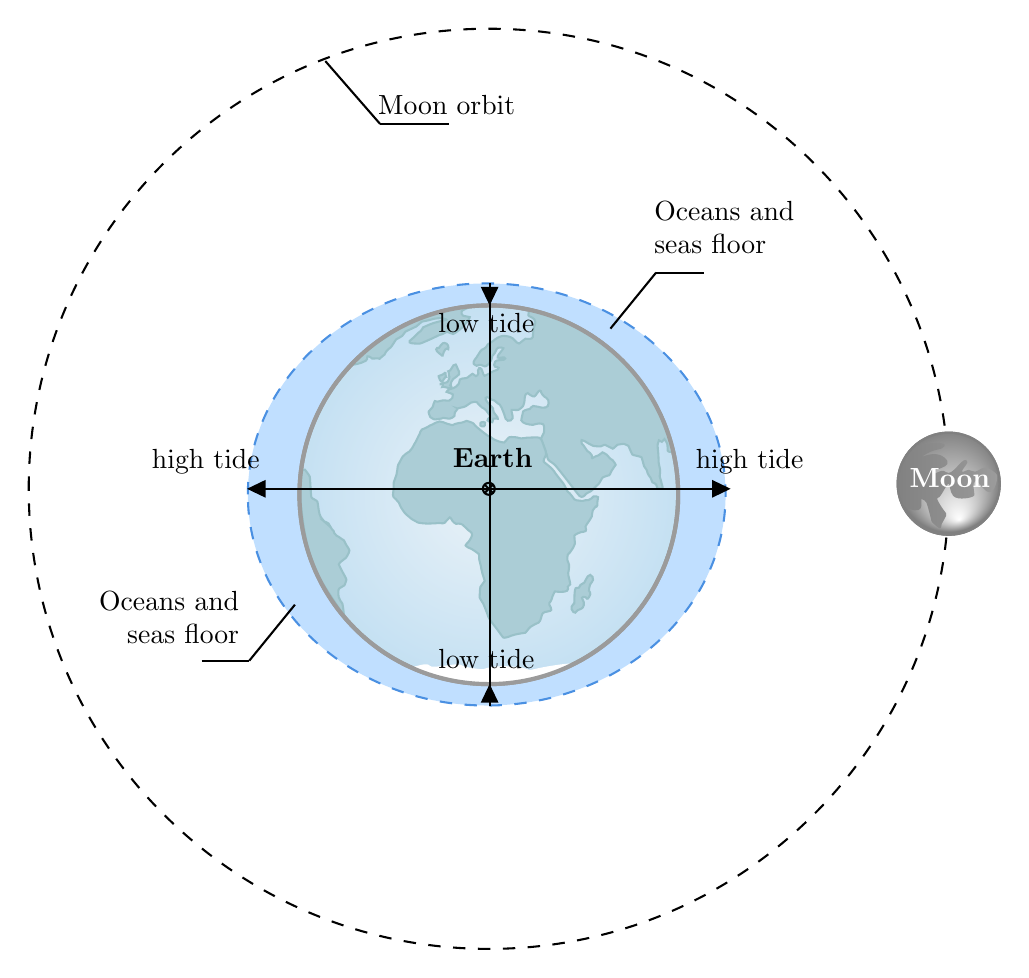
\begin{tikzpicture}[x=0.75pt,y=0.75pt,yscale=-1,xscale=1]
		%uncomment if require: \path (0,518); %set diagram left start at 0, and has height of 518
		
		%Shape: Ellipse [id:dp1564433669634886] 
		\draw  [color={rgb, 255:red, 74; green, 144; blue, 226 }  ,draw opacity=1 ][fill={rgb, 255:red, 192; green, 223; blue, 255 }  ,fill opacity=1 ][dash pattern={on 4.5pt off 4.5pt}] (207.67,244.82) .. controls (207.67,188.66) and (259.2,143.14) .. (322.76,143.14) .. controls (386.32,143.14) and (437.85,188.66) .. (437.85,244.82) .. controls (437.85,300.98) and (386.32,346.5) .. (322.76,346.5) .. controls (259.2,346.5) and (207.67,300.98) .. (207.67,244.82) -- cycle ;
		%Shape: Circle [id:dp9228061059909327] 
		\draw  [dash pattern={on 4.5pt off 4.5pt}] (102.1,242.09) .. controls (102.1,119.66) and (201.35,20.42) .. (323.78,20.42) .. controls (446.2,20.42) and (545.45,119.66) .. (545.45,242.09) .. controls (545.45,364.51) and (446.2,463.76) .. (323.78,463.76) .. controls (201.35,463.76) and (102.1,364.51) .. (102.1,242.09) -- cycle ;
		%Shape: Circle [id:dp8938982774548756] 
		\path  [shading=_5qwjotkth,_bq0bl2g2v] (232.55,244.96) .. controls (232.55,194.58) and (273.39,153.73) .. (323.78,153.73) .. controls (374.16,153.73) and (415,194.58) .. (415,244.96) .. controls (415,295.34) and (374.16,336.18) .. (323.78,336.18) .. controls (273.39,336.18) and (232.55,295.34) .. (232.55,244.96) -- cycle ; % for fading 
		 \draw  [color={rgb, 255:red, 155; green, 155; blue, 155 }  ,draw opacity=1 ][line width=1.5]  (232.55,244.96) .. controls (232.55,194.58) and (273.39,153.73) .. (323.78,153.73) .. controls (374.16,153.73) and (415,194.58) .. (415,244.96) .. controls (415,295.34) and (374.16,336.18) .. (323.78,336.18) .. controls (273.39,336.18) and (232.55,295.34) .. (232.55,244.96) -- cycle ; % for border 
		
		%Shape: Polygon Curved [id:ds03522640822952505] 
		\draw  [color={rgb, 255:red, 153; green, 193; blue, 200 }  ,draw opacity=1 ][fill={rgb, 255:red, 171; green, 205; blue, 214 }  ,fill opacity=1 ] (365.27,290.94) .. controls (365.63,288.89) and (366.48,290.46) .. (367.2,289.73) .. controls (367.93,289.01) and (367.27,289.03) .. (367.93,288.4) .. controls (368.59,287.78) and (369.02,287.88) .. (369.75,287.31) .. controls (370.49,286.73) and (370.24,285.92) .. (370.72,285.49) .. controls (371.2,285.07) and (371.56,283.33) .. (372.66,283.56) .. controls (373.75,283.79) and (374.02,285.16) .. (373.99,285.98) .. controls (373.95,286.79) and (372.98,287.22) .. (372.53,288.27) .. controls (372.09,289.32) and (372.06,290.87) .. (372.04,291.19) .. controls (372.02,291.5) and (373.38,292.14) .. (372.17,294.08) .. controls (370.96,296.01) and (371.08,294.63) .. (370.36,294.32) .. controls (369.64,294.01) and (368.96,294.12) .. (368.67,294.56) .. controls (368.37,295) and (370,296.13) .. (369.51,298.19) .. controls (369.03,300.24) and (367.86,299.75) .. (366.61,300.6) .. controls (365.36,301.45) and (365.38,302.56) .. (364.54,301.46) .. controls (363.71,300.36) and (363.34,299.95) .. (363.71,298.79) .. controls (364.08,297.63) and (364.77,297.86) .. (364.92,297.34) .. controls (365.07,296.82) and (364.91,293) .. (365.27,290.94) -- cycle ;
		%Shape: Polygon Curved [id:ds5157320992246872] 
		\draw  [color={rgb, 255:red, 153; green, 193; blue, 200 }  ,draw opacity=1 ][fill={rgb, 255:red, 171; green, 205; blue, 214 }  ,fill opacity=1 ] (301.56,171.98) .. controls (302.42,171.42) and (304.46,172.18) .. (304.34,174.11) .. controls (304.22,176.04) and (303.93,173.6) .. (302.76,175) .. controls (301.6,176.4) and (301.68,178.58) .. (301.19,177.9) .. controls (300.71,177.22) and (298.56,176.24) .. (298.41,174.96) .. controls (298.26,173.67) and (299.36,174.61) .. (299.74,174.23) .. controls (300.12,173.86) and (300.69,172.53) .. (301.56,171.98) -- cycle ;
		%Shape: Polygon Curved [id:ds1955429013119243] 
		\draw  [color={rgb, 255:red, 153; green, 193; blue, 200 }  ,draw opacity=1 ][fill={rgb, 255:red, 171; green, 205; blue, 214 }  ,fill opacity=1 ] (321.25,209.91) .. controls (322.12,209.35) and (321.98,210.63) .. (321.86,211.48) .. controls (321.73,212.33) and (321.13,211.96) .. (320.4,211.96) .. controls (319.68,211.96) and (319.56,211.48) .. (319.68,210.51) .. controls (319.8,209.54) and (320.39,210.46) .. (321.25,209.91) -- cycle ;
		%Shape: Polygon Curved [id:ds4612751901702774] 
		\draw  [color={rgb, 255:red, 153; green, 193; blue, 200 }  ,draw opacity=1 ][fill={rgb, 255:red, 171; green, 205; blue, 214 }  ,fill opacity=1 ] (283.77,163.13) .. controls (287.52,161.44) and (301.97,156.47) .. (304.87,155.87) .. controls (307.78,155.26) and (308.68,154.95) .. (310.97,154.67) .. controls (313.27,154.38) and (316.9,154.28) .. (315.57,154.43) .. controls (314.23,154.57) and (311.33,155.81) .. (310.73,156.48) .. controls (310.13,157.15) and (311.01,158.49) .. (311.34,158.66) .. controls (311.67,158.82) and (314.45,159.27) .. (314.6,159.38) .. controls (314.76,159.5) and (313.46,161.39) .. (313.03,161.92) .. controls (312.6,162.45) and (310.67,164.77) .. (310.01,165.19) .. controls (309.34,165.6) and (307,167.57) .. (306.5,167.48) .. controls (306,167.39) and (304.11,166.57) .. (303.72,166.52) .. controls (303.33,166.46) and (301.44,167.69) .. (300.82,167.72) .. controls (300.2,167.75) and (297.42,169.23) .. (296.93,169.44) .. controls (296.44,169.64) and (291.23,172.06) .. (290.64,172.1) .. controls (290.05,172.14) and (285.87,172.19) .. (285.65,171.58) .. controls (285.43,170.98) and (285.52,170.82) .. (286.74,169.89) .. controls (287.96,168.96) and (289.53,166.9) .. (290.85,166.14) .. controls (292.17,165.39) and (291.54,164.56) .. (292.06,164.33) .. controls (292.58,164.09) and (294.4,163.32) .. (295.6,162.79) .. controls (296.79,162.26) and (297.94,161.99) .. (299.47,161.58) .. controls (301,161.17) and (303.05,160.72) .. (303.3,160.58) .. controls (303.56,160.44) and (301.32,159.85) .. (300.88,159.85) .. controls (300.45,159.86) and (298.23,159.85) .. (296.29,160.46) .. controls (294.36,161.06) and (291.82,161.48) .. (291.58,161.55) .. controls (291.33,161.62) and (289.06,163.79) .. (288.67,163.97) .. controls (288.29,164.14) and (283.66,166.3) .. (283.6,166.38) .. controls (283.53,166.46) and (282.5,167.85) .. (282.02,168.44) .. controls (281.55,169.03) and (279.78,169.55) .. (279.24,170.01) .. controls (278.7,170.47) and (277.07,173.52) .. (276.46,174) .. controls (275.86,174.48) and (275.15,174.94) .. (274.53,175.69) .. controls (273.9,176.45) and (273.62,177.31) .. (273.56,177.39) .. controls (273.5,177.46) and (271.15,179.31) .. (271.14,179.44) .. controls (271.14,179.57) and (269.4,178.75) .. (268.48,179.32) .. controls (267.57,179.89) and (267.69,179.03) .. (266.07,178.35) .. controls (264.44,177.67) and (265.87,179.56) .. (264.49,180.41) .. controls (263.12,181.25) and (261.6,181.6) .. (260.14,181.98) .. controls (258.69,182.36) and (258.13,182.35) .. (258.09,181.97) .. controls (258.04,181.59) and (267.33,173.14) .. (268.36,172.66) .. controls (269.4,172.18) and (280.02,164.82) .. (283.77,163.13) -- cycle ;
		%Shape: Polygon Curved [id:ds3657837033917619] 
		\draw  [color={rgb, 255:red, 153; green, 193; blue, 200 }  ,draw opacity=1 ][fill={rgb, 255:red, 171; green, 205; blue, 214 }  ,fill opacity=1 ] (304.81,188.13) .. controls (304.73,187.27) and (304.33,187.89) .. (304.57,186.68) .. controls (304.81,185.47) and (303.87,185.69) .. (304.2,185.47) .. controls (304.54,185.26) and (305.9,185.11) .. (305.9,183.91) .. controls (305.9,182.7) and (307.47,182.18) .. (307.83,182.21) .. controls (308.2,182.24) and (308.28,183.57) .. (308.8,184.27) .. controls (309.31,184.97) and (309.67,186.12) .. (309.4,186.93) .. controls (309.13,187.73) and (307.96,187.88) .. (307.59,188.5) .. controls (307.22,189.11) and (305.95,189.07) .. (305.78,190.43) .. controls (305.6,191.79) and (305.25,192.01) .. (305.17,192.25) .. controls (305.09,192.48) and (306.02,192.12) .. (305.78,192.97) .. controls (305.7,193.24) and (305.52,193.4) .. (305.26,193.48) .. controls (304.71,193.64) and (303.78,193.42) .. (302.63,193.09) .. controls (300.94,192.61) and (301.16,193.68) .. (301.67,192.25) .. controls (302.17,190.81) and (300.02,192.12) .. (300.58,191.52) .. controls (301.14,190.92) and (303.76,191.24) .. (304.08,190.31) .. controls (304.41,189.38) and (304.88,189) .. (304.81,188.13) -- cycle ;
		%Shape: Polygon Curved [id:ds2972959762730816] 
		\draw  [color={rgb, 255:red, 153; green, 193; blue, 200 }  ,draw opacity=1 ][fill={rgb, 255:red, 171; green, 205; blue, 214 }  ,fill opacity=1 ] (301.54,187.05) .. controls (302.41,186.49) and (303.12,185.35) .. (303,187.29) .. controls (302.87,189.22) and (303.81,187.15) .. (302.64,188.54) .. controls (301.48,189.94) and (301.42,190.99) .. (300.94,190.31) .. controls (300.46,189.63) and (300.12,190.27) .. (299.97,188.98) .. controls (299.82,187.69) and (299.24,188.15) .. (299.62,187.77) .. controls (300,187.4) and (300.68,187.6) .. (301.54,187.05) -- cycle ;
		%Shape: Polygon Curved [id:ds30547861733844095] 
		\draw  [color={rgb, 255:red, 153; green, 193; blue, 200 }  ,draw opacity=1 ][fill={rgb, 255:red, 171; green, 205; blue, 214 }  ,fill opacity=1 ] (233.04,247.38) .. controls (232.91,245.48) and (233.04,233.6) .. (234.12,233) .. controls (235.21,232.39) and (235.26,233.03) .. (235.94,233.85) .. controls (236.62,234.66) and (237.33,235.85) .. (237.51,236.26) .. controls (237.69,236.67) and (237.99,245.57) .. (238.36,246.3) .. controls (238.72,247.02) and (241.02,247.51) .. (241.26,248.47) .. controls (241.5,249.44) and (241.86,254.52) .. (242.83,255.73) .. controls (243.8,256.94) and (244.47,257.79) .. (244.52,257.9) .. controls (244.57,258.02) and (243.86,257.38) .. (245.13,258.03) .. controls (246.39,258.67) and (246.94,258.75) .. (247.3,260.08) .. controls (247.66,261.41) and (248.94,262.21) .. (248.99,262.38) .. controls (249.05,262.55) and (249.24,264.23) .. (250.45,264.68) .. controls (251.65,265.12) and (253.35,266.81) .. (253.71,266.73) .. controls (254.07,266.65) and (254.51,268.39) .. (255.16,269.27) .. controls (255.81,270.15) and (256.49,271.08) .. (256.61,271.81) .. controls (256.73,272.53) and (255.77,273.82) .. (255.64,274.23) .. controls (255.52,274.64) and (254.64,276) .. (253.71,276.28) .. controls (252.78,276.56) and (251.59,278.23) .. (251.53,278.46) .. controls (251.48,278.69) and (253.3,282.19) .. (253.59,282.69) .. controls (253.88,283.19) and (255.35,285.74) .. (255.16,286.06) .. controls (254.97,286.39) and (254.42,288.45) .. (254.19,288.6) .. controls (253.97,288.75) and (252.55,289.57) .. (251.78,290.05) .. controls (251,290.54) and (251.29,292.71) .. (251.41,294.16) .. controls (251.53,295.61) and (252.98,296.58) .. (253.23,297.43) .. controls (253.47,298.27) and (254.06,303.16) .. (253.95,303.11) .. controls (253.84,303.06) and (243.31,287.39) .. (241.86,284.49) .. controls (240.41,281.59) and (237.11,273.54) .. (235.57,265.87) .. controls (234.04,258.21) and (233.17,249.27) .. (233.04,247.38) -- cycle ;
		%Shape: Polygon Curved [id:ds8162582902550839] 
		\draw  [color={rgb, 255:red, 153; green, 193; blue, 200 }  ,draw opacity=1 ][fill={rgb, 255:red, 171; green, 205; blue, 214 }  ,fill opacity=1 ] (348.97,218.19) .. controls (348.77,217.52) and (350.11,216.02) .. (350.3,215.05) .. controls (350.49,214.08) and (350.73,211.24) .. (349.7,210.82) .. controls (348.66,210.4) and (347.33,210.65) .. (346.37,210.89) .. controls (345.4,211.12) and (344.67,211.61) .. (343.46,211.13) .. controls (342.25,210.64) and (340.8,210.89) .. (340.2,210.04) .. controls (339.59,209.19) and (338.92,208.95) .. (339.59,207.98) .. controls (340.27,207.02) and (339.69,205.7) .. (340.3,204.85) .. controls (340.9,204.01) and (343.38,203.69) .. (343.56,203.64) .. controls (343.74,203.6) and (344.17,202.31) .. (345.13,202.19) .. controls (346.1,202.07) and (345.93,202.17) .. (347.38,202.53) .. controls (348.83,202.9) and (349.92,203.26) .. (351.12,202.9) .. controls (352.33,202.53) and (352.33,202.05) .. (352.58,200.84) .. controls (352.82,199.63) and (352.2,198.95) .. (351.54,198.32) .. controls (350.88,197.7) and (350.76,198.18) .. (349.55,196.61) .. controls (348.34,195.04) and (349.31,194.67) .. (348.34,194.79) .. controls (347.38,194.92) and (346.59,197.26) .. (345.68,197.58) .. controls (344.78,197.9) and (342.63,196.07) .. (342.54,196) .. controls (342.45,195.94) and (341.09,196.37) .. (341.09,198.18) .. controls (341.09,199.99) and (340.58,201.79) .. (340.12,202.41) .. controls (339.67,203.03) and (338.64,203.68) .. (338.19,203.98) .. controls (337.74,204.28) and (335.27,203.99) .. (334.8,204.1) .. controls (334.34,204.22) and (335.53,207.13) .. (335.23,208.09) .. controls (334.93,209.06) and (333.81,209.53) .. (332.93,209.3) .. controls (332.06,209.08) and (331.42,207.57) .. (331.48,207.13) .. controls (331.55,206.68) and (330.78,205.41) .. (330.66,204.81) .. controls (330.54,204.2) and (330.3,203.48) .. (329.93,202.99) .. controls (329.57,202.51) and (329.17,201.73) .. (329.09,201.54) .. controls (329.01,201.35) and (328.12,201.27) .. (327.39,200.33) .. controls (326.67,199.4) and (326.18,199.44) .. (325.22,199.13) .. controls (324.26,198.81) and (323.76,197.75) .. (323.04,197.92) .. controls (322.33,198.08) and (321.89,198.21) .. (322.32,199.25) .. controls (322.74,200.29) and (323.77,200.94) .. (324.13,201.54) .. controls (324.49,202.15) and (326.25,203.12) .. (325.89,204.2) .. controls (325.53,205.29) and (328.82,207.97) .. (328.1,208.34) .. controls (327.37,208.7) and (326.35,207.75) .. (325.92,208.34) .. controls (325.5,208.92) and (325.81,209.92) .. (325.44,210.03) .. controls (325.06,210.14) and (323.35,209.76) .. (323.16,209.14) .. controls (322.98,208.51) and (323.79,208.16) .. (324.2,207.71) .. controls (324.6,207.26) and (324.32,206.38) .. (323.59,205.77) .. controls (322.87,205.17) and (323.1,205.32) .. (322.38,204.2) .. controls (321.66,203.09) and (321.18,203.66) .. (320.57,202.99) .. controls (319.96,202.33) and (319.27,201.82) .. (318.55,201.05) .. controls (317.82,200.28) and (318.47,200.4) .. (317.1,200.2) .. controls (315.72,200.01) and (314.87,200.79) .. (314.07,201.29) .. controls (313.28,201.79) and (312.26,202.74) .. (311.54,202.74) .. controls (310.81,202.74) and (308.02,203.64) .. (308.63,203.35) .. controls (309.25,203.05) and (307.89,204.71) .. (307.42,205.28) .. controls (306.96,205.85) and (307.62,206.49) .. (307.18,207.09) .. controls (306.74,207.7) and (305.28,208.18) .. (304.89,208.3) .. controls (304.49,208.43) and (301.48,207.68) .. (301.49,207.99) .. controls (301.5,208.31) and (298.47,208.58) .. (297.87,208.67) .. controls (297.27,208.75) and (295.55,207.55) .. (295.57,207.51) .. controls (295.58,207.47) and (294.49,205.28) .. (294.85,204.8) .. controls (295.21,204.31) and (296.55,202.92) .. (296.66,202.74) .. controls (296.78,202.57) and (297.51,199.89) .. (297.75,199.84) .. controls (297.99,199.79) and (298.83,200.17) .. (299.08,200.09) .. controls (299.33,200.01) and (300.78,199.67) .. (301.02,199.61) .. controls (301.26,199.55) and (302.38,199.41) .. (302.59,199.49) .. controls (302.8,199.57) and (304.41,199.7) .. (304.64,199.61) .. controls (304.88,199.52) and (306.22,198.44) .. (306.22,198.29) .. controls (306.22,198.14) and (306.46,196.8) .. (306.46,196.6) .. controls (306.45,196.39) and (303.53,195.48) .. (303.43,195.39) .. controls (303.34,195.3) and (304.36,194.17) .. (304.64,194.18) .. controls (304.93,194.19) and (306.16,193.67) .. (306.34,193.7) .. controls (306.51,193.72) and (308.13,192.86) .. (308.15,192.73) .. controls (308.17,192.59) and (309.36,191.57) .. (309.36,191.4) .. controls (309.36,191.22) and (309.79,189.63) .. (309.84,189.46) .. controls (309.9,189.3) and (311.61,188.65) .. (311.78,188.86) .. controls (311.94,189.07) and (313.6,188.61) .. (313.71,188.38) .. controls (313.82,188.14) and (315.68,186.78) .. (315.89,186.69) .. controls (316.09,186.61) and (317.27,187.65) .. (317.46,187.78) .. controls (317.65,187.91) and (318.96,187.22) .. (318.73,186.5) .. controls (318.51,185.78) and (318.37,184.44) .. (319.1,183.96) .. controls (319.82,183.47) and (320.79,185.05) .. (320.79,185.77) .. controls (320.79,186.5) and (321.5,187.6) .. (321.69,187.66) .. controls (321.88,187.72) and (323.11,186.93) .. (323.5,186.82) .. controls (323.9,186.7) and (325.78,185.35) .. (326.71,185.17) .. controls (327.65,184.98) and (328.63,184.47) .. (328.52,183.79) .. controls (328.41,183.11) and (327.4,183.75) .. (326.71,183.23) .. controls (326.03,182.72) and (326.35,182.02) .. (326.83,180.81) .. controls (327.32,179.61) and (331.85,180.51) .. (331.66,179.32) .. controls (331.47,178.13) and (328.85,179.39) .. (328.04,178.88) .. controls (327.24,178.37) and (330.97,174.67) .. (330.75,174.38) .. controls (330.52,174.1) and (329.18,173.78) .. (328.21,174.14) .. controls (327.24,174.51) and (327.01,176.67) .. (326.23,177.19) .. controls (325.45,177.7) and (325.38,178.28) .. (325.02,179.85) .. controls (324.66,181.42) and (323.25,182.38) .. (322.48,182.99) .. controls (321.71,183.6) and (319.95,181.88) .. (319.22,182.39) .. controls (318.48,182.89) and (317.32,183.15) .. (316.56,182.02) .. controls (315.8,180.89) and (317.82,178.88) .. (317.81,178.86) .. controls (317.81,178.84) and (318.92,177.1) .. (319.02,176.92) .. controls (319.12,176.75) and (320.18,174.77) .. (321.39,174.65) .. controls (322.6,174.53) and (322.45,173.23) .. (323.25,172.57) .. controls (324.05,171.91) and (325.97,170.96) .. (326.88,170.03) .. controls (327.78,169.11) and (328.97,168.98) .. (329.78,168.58) .. controls (330.59,168.18) and (332.98,168.67) .. (333.17,168.7) .. controls (333.35,168.74) and (335.48,169.29) .. (336.07,170.4) .. controls (336.65,171.5) and (338.19,172.09) .. (338.36,172.09) .. controls (338.54,172.09) and (341.23,169.79) .. (341.39,169.79) .. controls (341.55,169.79) and (343.64,170) .. (344.41,169.67) .. controls (345.18,169.34) and (344.97,168.42) .. (345.01,168.34) .. controls (345.05,168.26) and (345.23,165.32) .. (345.26,165.2) .. controls (345.28,165.07) and (346.1,162.66) .. (346.22,161.93) .. controls (346.34,161.21) and (345.45,159.68) .. (344.53,159.51) .. controls (343.61,159.35) and (342.86,158.61) .. (342.84,158.55) .. controls (342.81,158.48) and (343.1,156.06) .. (343.1,156.01) .. controls (343.1,155.96) and (367.64,160.01) .. (388.32,180.56) .. controls (408.99,201.11) and (412.74,224.12) .. (412.74,224.18) .. controls (412.74,224.24) and (409.96,224.66) .. (409.96,223.69) .. controls (409.96,222.72) and (409.84,221.51) .. (409.84,220.91) .. controls (409.84,220.3) and (408.55,218.18) .. (408.39,218.13) .. controls (408.23,218.08) and (407.51,219.4) .. (407.18,219.46) .. controls (406.84,219.51) and (405.77,218.66) .. (405.73,218.73) .. controls (405.69,218.8) and (405.16,220.64) .. (405.12,220.79) .. controls (405.09,220.94) and (405.18,223.05) .. (405.24,223.33) .. controls (405.3,223.61) and (405.5,225.77) .. (405.5,226.23) .. controls (405.49,226.68) and (405.62,228.91) .. (405.61,229.37) .. controls (405.6,229.84) and (406.17,232.03) .. (406.33,233) .. controls (406.49,233.97) and (406.04,235.61) .. (406.09,236.02) .. controls (406.14,236.43) and (406.99,238.89) .. (406.94,239.17) .. controls (406.88,239.44) and (407.98,241.73) .. (407.3,241.95) .. controls (406.62,242.16) and (405.49,242.01) .. (405.24,242.07) .. controls (404.99,242.12) and (404.53,240.27) .. (404.4,240.01) .. controls (404.27,239.75) and (403,239) .. (402.7,239.04) .. controls (402.41,239.09) and (401.86,236.55) .. (401.37,236.26) .. controls (400.89,235.98) and (399.99,234.06) .. (400.04,233.6) .. controls (400.1,233.15) and (398.8,231.69) .. (398.59,231.19) .. controls (398.39,230.68) and (397.59,227.47) .. (397.38,226.97) .. controls (397.18,226.46) and (393.46,226.01) .. (393.03,225.64) .. controls (392.6,225.27) and (391.26,221.82) .. (391.1,221.52) .. controls (390.94,221.23) and (389.02,220.46) .. (388.8,220.44) .. controls (388.58,220.41) and (385.87,220.78) .. (385.66,220.92) .. controls (385.44,221.06) and (383.75,222.88) .. (383.48,222.73) .. controls (383.21,222.59) and (380.11,221.11) .. (379.85,220.92) .. controls (379.6,220.73) and (377.88,221.62) .. (377.68,221.65) .. controls (377.47,221.67) and (374.43,221.58) .. (374.05,221.4) .. controls (373.67,221.23) and (371.06,219.9) .. (370.91,219.71) .. controls (370.75,219.52) and (368.66,218.5) .. (368.49,218.6) .. controls (368.32,218.71) and (368.24,219.45) .. (368.61,220.41) .. controls (368.98,221.38) and (369.75,220.81) .. (370.18,222.35) .. controls (370.61,223.89) and (371.71,223.99) .. (372.48,224.77) .. controls (373.25,225.54) and (373.87,226.5) .. (373.45,227.19) .. controls (373.02,227.87) and (375.27,226.18) .. (376.59,225.98) .. controls (377.91,225.77) and (378.16,223.86) .. (379.13,224.77) .. controls (380.09,225.67) and (380.22,225.01) .. (381.31,226.46) .. controls (382.39,227.91) and (382.97,228) .. (383.24,228.15) .. controls (383.51,228.3) and (384.96,230.32) .. (384.88,230.53) .. controls (384.8,230.73) and (383.57,232.28) .. (382.88,233.47) .. controls (382.19,234.67) and (382.22,235.42) .. (381.79,235.53) .. controls (381.36,235.63) and (378.79,236.38) .. (378.52,236.74) .. controls (378.25,237.1) and (376.9,239.69) .. (376.57,239.86) .. controls (376.25,240.03) and (373.75,242.69) .. (373.45,242.78) .. controls (373.15,242.87) and (372.72,243.75) .. (371.51,243.99) .. controls (370.3,244.23) and (370.32,245.05) .. (370.18,245.08) .. controls (370.04,245.11) and (368.75,246.8) .. (367.47,245.52) .. controls (366.19,244.24) and (356.34,230.89) .. (355.02,230.04) .. controls (353.69,229.2) and (352.07,228.27) .. (351.99,227.02) .. controls (351.91,225.77) and (349.17,218.87) .. (348.97,218.19) -- cycle ;
		%Shape: Polygon Curved [id:ds7615015936100842] 
		\draw  [color={rgb, 255:red, 153; green, 193; blue, 200 }  ,draw opacity=1 ][fill={rgb, 255:red, 171; green, 205; blue, 214 }  ,fill opacity=1 ] (348.97,218.19) .. controls (349.7,219.47) and (350.67,222.76) .. (351.11,223.76) .. controls (351.55,224.76) and (351.52,226.17) .. (350.83,226.82) .. controls (350.14,227.46) and (350.3,228.68) .. (350.19,228.95) .. controls (350.08,229.23) and (354.18,231.86) .. (355.15,233.55) .. controls (356.11,235.24) and (359.06,238.64) .. (359.69,239.52) .. controls (360.31,240.4) and (361.12,242.34) .. (361.62,243.26) .. controls (362.12,244.19) and (363.55,244.47) .. (363.92,245.68) .. controls (364.28,246.89) and (365.48,247.6) .. (365.97,247.62) .. controls (366.46,247.63) and (368.98,248.09) .. (369.24,247.86) .. controls (369.49,247.63) and (370.99,247.56) .. (371.78,247.5) .. controls (372.56,247.43) and (373.47,246.42) .. (374.19,245.8) .. controls (374.92,245.19) and (376.36,246.09) .. (376.38,246.1) .. controls (376.4,246.12) and (376.21,248.01) .. (376.13,248.1) .. controls (376.05,248.19) and (376.14,249.14) .. (376.04,250.08) .. controls (375.95,251.02) and (375.32,250.59) .. (375.28,250.64) .. controls (375.24,250.69) and (374.41,251.65) .. (373.86,252.5) .. controls (373.32,253.35) and (373.81,254.52) .. (373.38,255.4) .. controls (372.95,256.28) and (372.4,257.08) .. (371.93,257.82) .. controls (371.46,258.55) and (370.42,259.76) .. (370.37,260.25) .. controls (370.31,260.73) and (371.34,262.77) .. (369.52,262.77) .. controls (367.71,262.77) and (365.18,264.22) .. (365.05,264.59) .. controls (364.92,264.96) and (365.23,267.87) .. (365.29,268.21) .. controls (365.36,268.56) and (364.26,270.84) .. (364.08,270.99) .. controls (363.91,271.15) and (362.64,273.29) .. (362.15,273.41) .. controls (361.66,273.54) and (361.22,276.45) .. (362.03,277.52) .. controls (362.84,278.59) and (362.27,281.75) .. (362.03,282.6) .. controls (361.79,283.45) and (363.29,288.01) .. (362.99,288.14) .. controls (362.7,288.27) and (361.9,289.22) .. (361.83,289.3) .. controls (361.75,289.37) and (362.71,291.39) .. (360.21,291.65) .. controls (357.71,291.91) and (355.8,291.53) .. (355.62,291.53) .. controls (355.45,291.53) and (354.47,293.94) .. (354.41,294.06) .. controls (354.35,294.19) and (353.87,296.39) .. (352.96,297.09) .. controls (352.05,297.79) and (355.75,300.73) .. (352.61,301.09) .. controls (349.46,301.45) and (349.63,302.51) .. (349.46,302.54) .. controls (349.3,302.56) and (348.91,305.85) .. (347.77,306.53) .. controls (346.63,307.21) and (345.25,307.46) .. (343.9,308.58) .. controls (342.55,309.7) and (341.73,311.4) .. (341.24,311.46) .. controls (340.75,311.52) and (336.04,312.19) .. (334.47,312.91) .. controls (332.9,313.64) and (331.18,313.97) .. (330.8,313.79) .. controls (330.42,313.62) and (327.7,309.53) .. (326.86,308.56) .. controls (326.01,307.59) and (323.42,303.96) .. (323.47,303.63) .. controls (323.52,303.3) and (321.21,297.61) .. (321.05,297.34) .. controls (320.9,297.07) and (319.38,294.75) .. (319.36,294.44) .. controls (319.34,294.13) and (319.52,289.65) .. (319.72,289.36) .. controls (319.92,289.07) and (321.74,286.58) .. (321.78,286.46) .. controls (321.82,286.34) and (320.91,283.6) .. (320.81,283.32) .. controls (320.72,283.04) and (320.03,280.16) .. (320.04,279.83) .. controls (320.05,279.5) and (319.34,277.26) .. (319.12,275.84) .. controls (318.9,274.43) and (319.32,273.82) .. (319,273.54) .. controls (318.67,273.27) and (317.58,272.45) .. (316.7,271.85) .. controls (315.82,271.25) and (314.98,270.75) .. (314.77,270.76) .. controls (314.56,270.78) and (312.79,269.84) .. (312.59,269.43) .. controls (312.39,269.03) and (314.1,267.75) .. (314.52,266.9) .. controls (314.95,266.04) and (315.64,265.2) .. (315.73,264.36) .. controls (315.83,263.51) and (315.13,263.03) .. (315.09,262.91) .. controls (315.04,262.78) and (313.31,261.79) .. (312.47,260.65) .. controls (311.63,259.52) and (310.63,259.12) .. (310.29,258.96) .. controls (309.95,258.8) and (308.24,258.88) .. (308,258.96) .. controls (307.75,259.04) and (306.4,257.89) .. (306.3,257.63) .. controls (306.2,257.37) and (305.18,255.62) .. (304.93,255.89) .. controls (304.68,256.17) and (302.91,257.97) .. (302.43,258.48) .. controls (301.96,258.98) and (299.62,258.43) .. (299.05,258.6) .. controls (298.48,258.77) and (294.91,258.81) .. (294.33,258.84) .. controls (293.76,258.87) and (289.84,258.59) .. (289.38,258.23) .. controls (288.92,257.88) and (286.73,256.8) .. (286.48,256.54) .. controls (286.22,256.29) and (283.91,254.45) .. (283.41,253.86) .. controls (282.91,253.27) and (281.35,251.05) .. (281.11,250.35) .. controls (280.87,249.66) and (280.27,247.94) .. (279.18,247.33) .. controls (278.09,246.73) and (277.24,245.76) .. (277.73,243.7) .. controls (278.21,241.65) and (277.36,239.47) .. (278.57,237.3) .. controls (279.78,235.12) and (279.69,230.92) .. (280.15,230.41) .. controls (280.6,229.89) and (281.52,227.75) .. (282.24,226.66) .. controls (282.97,225.57) and (284.26,224.96) .. (285.51,224.12) .. controls (286.76,223.27) and (287,221.82) .. (287.93,220.49) .. controls (288.85,219.16) and (289.86,216.48) .. (290.34,215.92) .. controls (290.83,215.36) and (290.67,213.81) .. (291.55,213.5) .. controls (292.44,213.19) and (294.33,212.34) .. (294.7,212.05) .. controls (295.06,211.76) and (295.8,211.36) .. (296.63,211.08) .. controls (297.46,210.81) and (298.81,209.63) .. (300.02,209.63) .. controls (301.23,209.63) and (302.23,210.27) .. (303.64,210.72) .. controls (305.06,211.17) and (306.32,211.42) .. (306.38,211.42) .. controls (306.44,211.43) and (308.12,210.26) .. (309.45,210.36) .. controls (310.77,210.46) and (312.85,209.4) .. (313.03,209.37) .. controls (313.21,209.34) and (316.25,210.31) .. (316.34,210.6) .. controls (316.43,210.89) and (318.46,212.83) .. (318.64,212.9) .. controls (318.81,212.97) and (320.88,214.74) .. (321.17,214.95) .. controls (321.47,215.16) and (322.67,215.98) .. (322.75,216.16) .. controls (322.82,216.34) and (323.86,216.83) .. (324.32,216.89) .. controls (324.78,216.94) and (325.55,218.3) .. (326.49,218.46) .. controls (327.44,218.62) and (327.48,218.81) .. (328.15,219.1) .. controls (328.83,219.4) and (330.85,219.84) .. (331.16,219.77) .. controls (331.48,219.69) and (333.09,217.49) .. (333.63,217.25) .. controls (334.17,217.01) and (337.38,217.14) .. (338.34,217.61) .. controls (339.3,218.09) and (341.9,217.45) .. (342.05,217.47) .. controls (342.19,217.49) and (344.9,217.33) .. (345.31,217.35) .. controls (345.72,217.37) and (348.24,216.92) .. (348.97,218.19) -- cycle ;
		%Flowchart: Summing Junction [id:dp5351361757951671] 
		\draw   (320.91,242.09) .. controls (320.91,240.5) and (322.19,239.22) .. (323.78,239.22) .. controls (325.36,239.22) and (326.65,240.5) .. (326.65,242.09) .. controls (326.65,243.67) and (325.36,244.96) .. (323.78,244.96) .. controls (322.19,244.96) and (320.91,243.67) .. (320.91,242.09) -- cycle ; \draw   (321.75,240.06) -- (325.81,244.12) ; \draw   (325.81,240.06) -- (321.75,244.12) ;
		%Shape: Polygon Curved [id:ds10402683200446483] 
		\draw  [draw opacity=0][fill={rgb, 255:red, 255; green, 255; blue, 255 }  ,fill opacity=1 ] (286.24,328.03) .. controls (287.57,328.15) and (294.04,325.44) .. (295.25,327.26) .. controls (296.46,329.07) and (308.69,325.71) .. (310.26,326.92) .. controls (311.83,328.13) and (320.35,329.23) .. (321.26,328.97) .. controls (322.18,328.71) and (325,327.11) .. (334.8,327.68) .. controls (344.6,328.25) and (341.03,330.16) .. (345.68,328.97) .. controls (350.34,327.78) and (363.38,325.73) .. (363.82,326.45) .. controls (364.26,327.18) and (368.38,324.06) .. (354.92,330.69) .. controls (341.45,337.31) and (307.64,337.58) .. (292.53,330.57) .. controls (277.42,323.55) and (284.92,327.91) .. (286.24,328.03) -- cycle ;
		%Shape: Circle [id:dp9728675388373518] 
		\draw  [color={rgb, 255:red, 155; green, 155; blue, 155 }  ,draw opacity=1 ][line width=1.5]  (232.55,244.96) .. controls (232.55,194.58) and (273.39,153.73) .. (323.78,153.73) .. controls (374.16,153.73) and (415,194.58) .. (415,244.96) .. controls (415,295.34) and (374.16,336.18) .. (323.78,336.18) .. controls (273.39,336.18) and (232.55,295.34) .. (232.55,244.96) -- cycle ;
		%Shape: Ellipse [id:dp06615245104559708] 
		\path  [shading=_4p2mskewt,_oe8oxlngv] (520.72,239.64) .. controls (520.72,226.03) and (531.75,215) .. (545.35,215) .. controls (558.96,215) and (569.99,226.03) .. (569.99,239.64) .. controls (569.99,253.24) and (558.96,264.27) .. (545.35,264.27) .. controls (531.75,264.27) and (520.72,253.24) .. (520.72,239.64) -- cycle ; % for fading 
		 \draw  [color={rgb, 255:red, 128; green, 128; blue, 128 }  ,draw opacity=1 ] (520.72,239.64) .. controls (520.72,226.03) and (531.75,215) .. (545.35,215) .. controls (558.96,215) and (569.99,226.03) .. (569.99,239.64) .. controls (569.99,253.24) and (558.96,264.27) .. (545.35,264.27) .. controls (531.75,264.27) and (520.72,253.24) .. (520.72,239.64) -- cycle ; % for border 
		
		%Shape: Polygon Curved [id:ds9750185079397313] 
		\draw  [draw opacity=0][shading=_k8rmnwma5,_o4o4l9od6] (532.05,221.38) .. controls (535.45,219.69) and (545.35,219.22) .. (543.19,221.69) .. controls (541.02,224.17) and (539.78,221.69) .. (532.36,226.64) .. controls (524.94,231.59) and (536.69,221.69) .. (543.19,226.95) .. controls (549.68,232.21) and (535.14,232.83) .. (537.31,234.38) .. controls (539.48,235.92) and (541.11,231.84) .. (544.12,234.07) .. controls (547.12,236.3) and (551.23,227.57) .. (553.71,228.19) .. controls (556.18,228.81) and (551.25,232.92) .. (551.85,233.76) .. controls (552.45,234.59) and (554.33,231.91) .. (556.49,233.45) .. controls (558.65,234.98) and (560.45,231.87) .. (562.68,231.9) .. controls (564.9,231.94) and (567.87,234.22) .. (568.55,235.31) .. controls (569.24,236.39) and (567.9,243.31) .. (565.15,243.66) .. controls (562.4,244.01) and (559.66,237.59) .. (558.04,238.4) .. controls (556.41,239.21) and (557.92,244.02) .. (557.73,245.2) .. controls (557.53,246.39) and (549.54,247.92) .. (547.52,245.51) .. controls (545.49,243.11) and (546.25,240.06) .. (545.35,239.64) .. controls (544.45,239.22) and (541.59,246.56) .. (540.09,246.44) .. controls (538.6,246.33) and (543.12,252.77) .. (544.12,253.87) .. controls (545.11,254.97) and (541.28,258.76) .. (541.64,260.67) .. controls (542,262.59) and (537.14,258.48) .. (537,257.58) .. controls (536.86,256.67) and (535.05,249.47) .. (534.53,248.61) .. controls (534.01,247.74) and (533.58,247.66) .. (532.36,247.06) .. controls (531.14,246.47) and (535.14,255.1) .. (526.17,251.7) .. controls (517.2,248.3) and (521.65,233.98) .. (523.08,231.28) .. controls (524.51,228.59) and (528.66,223.08) .. (532.05,221.38) -- cycle ;
		%Shape: Ellipse [id:dp41846841682358904] 
		\draw  [color={rgb, 255:red, 128; green, 128; blue, 128 }  ,draw opacity=1 ] (520.72,239.64) .. controls (520.72,226.03) and (531.75,215) .. (545.35,215) .. controls (558.96,215) and (569.99,226.03) .. (569.99,239.64) .. controls (569.99,253.24) and (558.96,264.27) .. (545.35,264.27) .. controls (531.75,264.27) and (520.72,253.24) .. (520.72,239.64) -- cycle ;
		%Straight Lines [id:da9868873952347357] 
		\draw    (210.28,242.09) -- (437.28,242.09) ;
		\draw [shift={(440.28,242.09)}, rotate = 180] [fill={rgb, 255:red, 0; green, 0; blue, 0 }  ][line width=0.08]  [draw opacity=0] (8.93,-4.29) -- (0,0) -- (8.93,4.29) -- cycle    ;
		\draw [shift={(207.28,242.09)}, rotate = 0] [fill={rgb, 255:red, 0; green, 0; blue, 0 }  ][line width=0.08]  [draw opacity=0] (8.93,-4.29) -- (0,0) -- (8.93,4.29) -- cycle    ;
		%Straight Lines [id:da3745316989766154] 
		\draw    (324.17,143.14) -- (324.17,346.5) ;
		%Straight Lines [id:da4412465250705735] 
		\draw    (324.17,143.14) -- (324.17,150.73) ;
		\draw [shift={(324.17,153.73)}, rotate = 270] [fill={rgb, 255:red, 0; green, 0; blue, 0 }  ][line width=0.08]  [draw opacity=0] (8.93,-4.29) -- (0,0) -- (8.93,4.29) -- cycle    ;
		%Straight Lines [id:da46366622161011994] 
		\draw    (324.17,346.5) -- (324.17,339.18) ;
		\draw [shift={(324.17,336.18)}, rotate = 90] [fill={rgb, 255:red, 0; green, 0; blue, 0 }  ][line width=0.08]  [draw opacity=0] (8.93,-4.29) -- (0,0) -- (8.93,4.29) -- cycle    ;
		%Straight Lines [id:da5573935825848315] 
		\draw    (245,36) -- (271.37,66.27) ;
		%Straight Lines [id:da24756334363402566] 
		\draw    (271.37,66.27) -- (304.37,66.27) ;
		%Straight Lines [id:da7621634747060604] 
		\draw    (404.37,137.91) -- (382.37,164.91) ;
		%Straight Lines [id:da751473715173612] 
		\draw    (404.37,137.91) -- (427.37,137.91) ;
		%Straight Lines [id:da4487945768391972] 
		\draw    (230.37,297.91) -- (208.37,324.91) ;
		%Straight Lines [id:da4593038227047086] 
		\draw    (185.37,324.91) -- (208.37,324.91) ;
		
		% Text Node
		\draw (305,221) node [anchor=north west][inner sep=0.75pt]   [align=left] {\textbf{Earth}};
		% Text Node
		\draw (525,231) node [anchor=north west][inner sep=0.75pt]  [color={rgb, 255:red, 255; green, 255; blue, 255 }  ,opacity=1 ] [align=left] {\textbf{Moon}};
		% Text Node
		\draw (269,51) node [anchor=north west][inner sep=0.75pt]   [align=left] {Moon orbit};
		% Text Node
		\draw (298,156) node [anchor=north west][inner sep=0.75pt]   [align=left] {low tide};
		% Text Node
		\draw (298,318) node [anchor=north west][inner sep=0.75pt]   [align=left] {low tide};
		% Text Node
		\draw (160,221.5) node [anchor=north west][inner sep=0.75pt]   [align=left] {high tide};
		% Text Node
		\draw (422,221.5) node [anchor=north west][inner sep=0.75pt]   [align=left] {high tide};
		% Text Node
		\draw (402,102) node [anchor=north west][inner sep=0.75pt]   [align=left] {Oceans and\\seas floor};
		% Text Node
		\draw (125,290) node [anchor=north west][inner sep=0.75pt]   [align=left] {\begin{minipage}[lt]{57.71pt}\setlength\topsep{0pt}
		\begin{flushright}
		Oceans and\\seas floor
		\end{flushright}
		\end{minipage}};
		\end{tikzpicture}
		\vspace*{3mm}
		\caption[]{Antipodal tide with antipodal bulge}
	\end{figure}
	If we considered the surface of the Earth as perfectly spherical and covered with water, it would then take the form of an ellipsoid whose axis would be directed to the celestial object generating the tide. We should then observe high tide and low tide that would take place twice a day and always at the same time. We name this the "\NewTerm{static tide}\index{static tide}" and the corresponding model "\NewTerm{static model of the tides}\index{static model of the tides}".
	
	\begin{tcolorbox}[enhanced,colback=red!5!white,colframe=black!50!red,boxrule=1pt,arc=0pt,outer arc=0pt,drop lifted shadow,after skip=10pt plus 2pt]
	\bcbombe The above figure is wrong even if we found it in many textbooks and even some TV show! The outgrowth is incorrectly placed - referred as the "Newtonian model of tides" - and should be rotated from $\pi/2$ as observed experimentally on our planet (there is almost no tides when the Moon is visible above us) and referred as the "Laplacian model of tides".
	\end{tcolorbox}

	It should be noted that the subtle play between the rotation of the Earth and the Moon produces enormous friction in water volume that have the effect of slowing the speed of rotation of the Earth about $1$ second every thousand years (this will result in a far future in a "\NewTerm{tidal lock}\index{tidal lock}\footnote{Tidal locking is the phenomenon by which a body has the same rotational period as its orbital period around a partner. So, the Moon is tidally locked to the Earth because it rotates in exactly the same time as it takes to orbit the Earth.}").
	\begin{figure}[H]
		\centering
		\includegraphics[width=1.0\textwidth]{img/engineering/vertical_horizontal_aspect_of_tides.jpg}
		\caption[]{Tides are visible in their horizontal component, not in their vertical one (a common misconception by many people) (source: Idées froides/YouTube)}
	\end{figure}
	The tides can be huge and varies a lot from area to area because they are simply horizontal waves, moving quite slowly in comparison to conventional waves (even  if they move as quick as a running average human), which behaviours depends strongly on the profile of the coasts and the depth of the water (see page \pageref{waves}). That's why most of the times, ocean tides are bigger than seas tides.
	
	The reflection of waves on the continents explains also why there are also sometimes only on tide per day or even more depending on the place on Earth... obviously of unequal amplitudes! As the reader can imagine, this is real life much more complicated because it is highly multi-factorial!
	
	\pagebreak
	\paragraph{Second approach}\mbox{}\\\\
	For the second approach, which is worth seeing for general culture and also because it presents another interesting aspect of the explanation of the attraction between two celestial objects, let us consider the following scheme where the Earth doesn't need to be considered as rigid:
	\begin{figure}[H]
		\centering
		% Gradient Info
  
		\tikzset {_24ypmjy6c/.code = {\pgfsetadditionalshadetransform{ \pgftransformshift{\pgfpoint{0 bp } { 0 bp }  }  \pgftransformscale{1 }  }}}
		\pgfdeclareradialshading{_jisg9oas4}{\pgfpoint{0bp}{0bp}}{rgb(0bp)=(0.92,0.95,0.97);
		rgb(0.08117079734802246bp)=(0.92,0.95,0.97);
		rgb(25bp)=(0.77,0.88,0.95);
		rgb(400bp)=(0.77,0.88,0.95)}
		
		% Gradient Info
		  
		\tikzset {_hn17qt2al/.code = {\pgfsetadditionalshadetransform{ \pgftransformshift{\pgfpoint{-75 bp } { 286.5 bp }  }  \pgftransformscale{1 }  }}}
		\pgfdeclareradialshading{_hkvbaiisa}{\pgfpoint{80bp}{-304bp}}{rgb(0bp)=(1,1,1);
		rgb(0bp)=(1,1,1);
		rgb(25bp)=(0.5,0.5,0.5);
		rgb(400bp)=(0.5,0.5,0.5)}
		
		% Gradient Info
		  
		\tikzset {_bfp99c13j/.code = {\pgfsetadditionalshadetransform{ \pgftransformshift{\pgfpoint{0 bp } { 0 bp }  }  \pgftransformrotate{0 }  \pgftransformscale{2 }  }}}
		\pgfdeclarehorizontalshading{_14cp0o8p5}{150bp}{rgb(0bp)=(0.5,0.5,0.5);
		rgb(37.5811653477805bp)=(0.5,0.5,0.5);
		rgb(62.49188508306231bp)=(0.61,0.61,0.61);
		rgb(100bp)=(0.61,0.61,0.61)}
		\tikzset{every picture/.style={line width=0.75pt}} %set default line width to 0.75pt        
		
		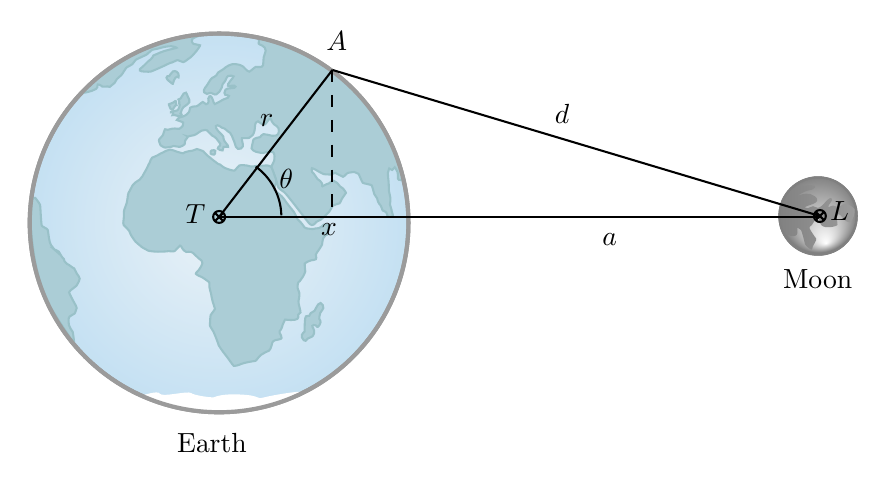
\begin{tikzpicture}[x=0.75pt,y=0.75pt,yscale=-1,xscale=1]
		%uncomment if require: \path (0,518); %set diagram left start at 0, and has height of 518
		
		%Shape: Circle [id:dp8938982774548756] 
		\path  [shading=_jisg9oas4,_24ypmjy6c] (114.55,158.96) .. controls (114.55,108.58) and (155.39,67.73) .. (205.78,67.73) .. controls (256.16,67.73) and (297,108.58) .. (297,158.96) .. controls (297,209.34) and (256.16,250.18) .. (205.78,250.18) .. controls (155.39,250.18) and (114.55,209.34) .. (114.55,158.96) -- cycle ; % for fading 
		 \draw  [color={rgb, 255:red, 155; green, 155; blue, 155 }  ,draw opacity=1 ][line width=1.5]  (114.55,158.96) .. controls (114.55,108.58) and (155.39,67.73) .. (205.78,67.73) .. controls (256.16,67.73) and (297,108.58) .. (297,158.96) .. controls (297,209.34) and (256.16,250.18) .. (205.78,250.18) .. controls (155.39,250.18) and (114.55,209.34) .. (114.55,158.96) -- cycle ; % for border 
		
		%Shape: Polygon Curved [id:ds03522640822952505] 
		\draw  [color={rgb, 255:red, 153; green, 193; blue, 200 }  ,draw opacity=1 ][fill={rgb, 255:red, 171; green, 205; blue, 214 }  ,fill opacity=1 ] (247.27,204.94) .. controls (247.63,202.89) and (248.48,204.46) .. (249.2,203.73) .. controls (249.93,203.01) and (249.27,203.03) .. (249.93,202.4) .. controls (250.59,201.78) and (251.02,201.88) .. (251.75,201.31) .. controls (252.49,200.73) and (252.24,199.92) .. (252.72,199.49) .. controls (253.2,199.07) and (253.56,197.33) .. (254.66,197.56) .. controls (255.75,197.79) and (256.02,199.16) .. (255.99,199.98) .. controls (255.95,200.79) and (254.98,201.22) .. (254.53,202.27) .. controls (254.09,203.32) and (254.06,204.87) .. (254.04,205.19) .. controls (254.02,205.5) and (255.38,206.14) .. (254.17,208.08) .. controls (252.96,210.01) and (253.08,208.63) .. (252.36,208.32) .. controls (251.64,208.01) and (250.96,208.12) .. (250.67,208.56) .. controls (250.37,209) and (252,210.13) .. (251.51,212.19) .. controls (251.03,214.24) and (249.86,213.75) .. (248.61,214.6) .. controls (247.36,215.45) and (247.38,216.56) .. (246.54,215.46) .. controls (245.71,214.36) and (245.34,213.95) .. (245.71,212.79) .. controls (246.08,211.63) and (246.77,211.86) .. (246.92,211.34) .. controls (247.07,210.82) and (246.91,207) .. (247.27,204.94) -- cycle ;
		%Shape: Polygon Curved [id:ds5157320992246872] 
		\draw  [color={rgb, 255:red, 153; green, 193; blue, 200 }  ,draw opacity=1 ][fill={rgb, 255:red, 171; green, 205; blue, 214 }  ,fill opacity=1 ] (183.56,85.98) .. controls (184.42,85.42) and (186.46,86.18) .. (186.34,88.11) .. controls (186.22,90.04) and (185.93,87.6) .. (184.76,89) .. controls (183.6,90.4) and (183.68,92.58) .. (183.19,91.9) .. controls (182.71,91.22) and (180.56,90.24) .. (180.41,88.96) .. controls (180.26,87.67) and (181.36,88.61) .. (181.74,88.23) .. controls (182.12,87.86) and (182.69,86.53) .. (183.56,85.98) -- cycle ;
		%Shape: Polygon Curved [id:ds1955429013119243] 
		\draw  [color={rgb, 255:red, 153; green, 193; blue, 200 }  ,draw opacity=1 ][fill={rgb, 255:red, 171; green, 205; blue, 214 }  ,fill opacity=1 ] (203.25,123.91) .. controls (204.12,123.35) and (203.98,124.63) .. (203.86,125.48) .. controls (203.73,126.33) and (203.13,125.96) .. (202.4,125.96) .. controls (201.68,125.96) and (201.56,125.48) .. (201.68,124.51) .. controls (201.8,123.54) and (202.39,124.46) .. (203.25,123.91) -- cycle ;
		%Shape: Polygon Curved [id:ds4612751901702774] 
		\draw  [color={rgb, 255:red, 153; green, 193; blue, 200 }  ,draw opacity=1 ][fill={rgb, 255:red, 171; green, 205; blue, 214 }  ,fill opacity=1 ] (165.77,77.13) .. controls (169.52,75.44) and (183.97,70.47) .. (186.87,69.87) .. controls (189.78,69.26) and (190.68,68.95) .. (192.97,68.67) .. controls (195.27,68.38) and (198.9,68.28) .. (197.57,68.43) .. controls (196.23,68.57) and (193.33,69.81) .. (192.73,70.48) .. controls (192.13,71.15) and (193.01,72.49) .. (193.34,72.66) .. controls (193.67,72.82) and (196.45,73.27) .. (196.6,73.38) .. controls (196.76,73.5) and (195.46,75.39) .. (195.03,75.92) .. controls (194.6,76.45) and (192.67,78.77) .. (192.01,79.19) .. controls (191.34,79.6) and (189,81.57) .. (188.5,81.48) .. controls (188,81.39) and (186.11,80.57) .. (185.72,80.52) .. controls (185.33,80.46) and (183.44,81.69) .. (182.82,81.72) .. controls (182.2,81.75) and (179.42,83.23) .. (178.93,83.44) .. controls (178.44,83.64) and (173.23,86.06) .. (172.64,86.1) .. controls (172.05,86.14) and (167.87,86.19) .. (167.65,85.58) .. controls (167.43,84.98) and (167.52,84.82) .. (168.74,83.89) .. controls (169.96,82.96) and (171.53,80.9) .. (172.85,80.14) .. controls (174.17,79.39) and (173.54,78.56) .. (174.06,78.33) .. controls (174.58,78.09) and (176.4,77.32) .. (177.6,76.79) .. controls (178.79,76.26) and (179.94,75.99) .. (181.47,75.58) .. controls (183,75.17) and (185.05,74.72) .. (185.3,74.58) .. controls (185.56,74.44) and (183.32,73.85) .. (182.88,73.85) .. controls (182.45,73.86) and (180.23,73.85) .. (178.29,74.46) .. controls (176.36,75.06) and (173.82,75.48) .. (173.58,75.55) .. controls (173.33,75.62) and (171.06,77.79) .. (170.67,77.97) .. controls (170.29,78.14) and (165.66,80.3) .. (165.6,80.38) .. controls (165.53,80.46) and (164.5,81.85) .. (164.02,82.44) .. controls (163.55,83.03) and (161.78,83.55) .. (161.24,84.01) .. controls (160.7,84.47) and (159.07,87.52) .. (158.46,88) .. controls (157.86,88.48) and (157.15,88.94) .. (156.53,89.69) .. controls (155.9,90.45) and (155.62,91.31) .. (155.56,91.39) .. controls (155.5,91.46) and (153.15,93.31) .. (153.14,93.44) .. controls (153.14,93.57) and (151.4,92.75) .. (150.48,93.32) .. controls (149.57,93.89) and (149.69,93.03) .. (148.07,92.35) .. controls (146.44,91.67) and (147.87,93.56) .. (146.49,94.41) .. controls (145.12,95.25) and (143.6,95.6) .. (142.14,95.98) .. controls (140.69,96.36) and (140.13,96.35) .. (140.09,95.97) .. controls (140.04,95.59) and (149.33,87.14) .. (150.36,86.66) .. controls (151.4,86.18) and (162.02,78.82) .. (165.77,77.13) -- cycle ;
		%Shape: Polygon Curved [id:ds3657837033917619] 
		\draw  [color={rgb, 255:red, 153; green, 193; blue, 200 }  ,draw opacity=1 ][fill={rgb, 255:red, 171; green, 205; blue, 214 }  ,fill opacity=1 ] (186.81,102.13) .. controls (186.73,101.27) and (186.33,101.89) .. (186.57,100.68) .. controls (186.81,99.47) and (185.87,99.69) .. (186.2,99.47) .. controls (186.54,99.26) and (187.9,99.11) .. (187.9,97.91) .. controls (187.9,96.7) and (189.47,96.18) .. (189.83,96.21) .. controls (190.2,96.24) and (190.28,97.57) .. (190.8,98.27) .. controls (191.31,98.97) and (191.67,100.12) .. (191.4,100.93) .. controls (191.13,101.73) and (189.96,101.88) .. (189.59,102.5) .. controls (189.22,103.11) and (187.95,103.07) .. (187.78,104.43) .. controls (187.6,105.79) and (187.25,106.01) .. (187.17,106.25) .. controls (187.09,106.48) and (188.02,106.12) .. (187.78,106.97) .. controls (187.7,107.24) and (187.52,107.4) .. (187.26,107.48) .. controls (186.71,107.64) and (185.78,107.42) .. (184.63,107.09) .. controls (182.94,106.61) and (183.16,107.68) .. (183.67,106.25) .. controls (184.17,104.81) and (182.02,106.12) .. (182.58,105.52) .. controls (183.14,104.92) and (185.76,105.24) .. (186.08,104.31) .. controls (186.41,103.38) and (186.88,103) .. (186.81,102.13) -- cycle ;
		%Shape: Polygon Curved [id:ds2972959762730816] 
		\draw  [color={rgb, 255:red, 153; green, 193; blue, 200 }  ,draw opacity=1 ][fill={rgb, 255:red, 171; green, 205; blue, 214 }  ,fill opacity=1 ] (183.54,101.05) .. controls (184.41,100.49) and (185.12,99.35) .. (185,101.29) .. controls (184.87,103.22) and (185.81,101.15) .. (184.64,102.54) .. controls (183.48,103.94) and (183.42,104.99) .. (182.94,104.31) .. controls (182.46,103.63) and (182.12,104.27) .. (181.97,102.98) .. controls (181.82,101.69) and (181.24,102.15) .. (181.62,101.77) .. controls (182,101.4) and (182.68,101.6) .. (183.54,101.05) -- cycle ;
		%Shape: Polygon Curved [id:ds30547861733844095] 
		\draw  [color={rgb, 255:red, 153; green, 193; blue, 200 }  ,draw opacity=1 ][fill={rgb, 255:red, 171; green, 205; blue, 214 }  ,fill opacity=1 ] (115.04,161.38) .. controls (114.91,159.48) and (115.04,147.6) .. (116.12,147) .. controls (117.21,146.39) and (117.26,147.03) .. (117.94,147.85) .. controls (118.62,148.66) and (119.33,149.85) .. (119.51,150.26) .. controls (119.69,150.67) and (119.99,159.57) .. (120.36,160.3) .. controls (120.72,161.02) and (123.02,161.51) .. (123.26,162.47) .. controls (123.5,163.44) and (123.86,168.52) .. (124.83,169.73) .. controls (125.8,170.94) and (126.47,171.79) .. (126.52,171.9) .. controls (126.57,172.02) and (125.86,171.38) .. (127.13,172.03) .. controls (128.39,172.67) and (128.94,172.75) .. (129.3,174.08) .. controls (129.66,175.41) and (130.94,176.21) .. (130.99,176.38) .. controls (131.05,176.55) and (131.24,178.23) .. (132.45,178.68) .. controls (133.65,179.12) and (135.35,180.81) .. (135.71,180.73) .. controls (136.07,180.65) and (136.51,182.39) .. (137.16,183.27) .. controls (137.81,184.15) and (138.49,185.08) .. (138.61,185.81) .. controls (138.73,186.53) and (137.77,187.82) .. (137.64,188.23) .. controls (137.52,188.64) and (136.64,190) .. (135.71,190.28) .. controls (134.78,190.56) and (133.59,192.23) .. (133.53,192.46) .. controls (133.48,192.69) and (135.3,196.19) .. (135.59,196.69) .. controls (135.88,197.19) and (137.35,199.74) .. (137.16,200.06) .. controls (136.97,200.39) and (136.42,202.45) .. (136.19,202.6) .. controls (135.97,202.75) and (134.55,203.57) .. (133.78,204.05) .. controls (133,204.54) and (133.29,206.71) .. (133.41,208.16) .. controls (133.53,209.61) and (134.98,210.58) .. (135.23,211.43) .. controls (135.47,212.27) and (136.06,217.16) .. (135.95,217.11) .. controls (135.84,217.06) and (125.31,201.39) .. (123.86,198.49) .. controls (122.41,195.59) and (119.11,187.54) .. (117.57,179.87) .. controls (116.04,172.21) and (115.17,163.27) .. (115.04,161.38) -- cycle ;
		%Shape: Polygon Curved [id:ds8162582902550839] 
		\draw  [color={rgb, 255:red, 153; green, 193; blue, 200 }  ,draw opacity=1 ][fill={rgb, 255:red, 171; green, 205; blue, 214 }  ,fill opacity=1 ] (230.97,132.19) .. controls (230.77,131.52) and (232.11,130.02) .. (232.3,129.05) .. controls (232.49,128.08) and (232.73,125.24) .. (231.7,124.82) .. controls (230.66,124.4) and (229.33,124.65) .. (228.37,124.89) .. controls (227.4,125.12) and (226.67,125.61) .. (225.46,125.13) .. controls (224.25,124.64) and (222.8,124.89) .. (222.2,124.04) .. controls (221.59,123.19) and (220.92,122.95) .. (221.59,121.98) .. controls (222.27,121.02) and (221.69,119.7) .. (222.3,118.85) .. controls (222.9,118.01) and (225.38,117.69) .. (225.56,117.64) .. controls (225.74,117.6) and (226.17,116.31) .. (227.13,116.19) .. controls (228.1,116.07) and (227.93,116.17) .. (229.38,116.53) .. controls (230.83,116.9) and (231.92,117.26) .. (233.12,116.9) .. controls (234.33,116.53) and (234.33,116.05) .. (234.58,114.84) .. controls (234.82,113.63) and (234.2,112.95) .. (233.54,112.32) .. controls (232.88,111.7) and (232.76,112.18) .. (231.55,110.61) .. controls (230.34,109.04) and (231.31,108.67) .. (230.34,108.79) .. controls (229.38,108.92) and (228.59,111.26) .. (227.68,111.58) .. controls (226.78,111.9) and (224.63,110.07) .. (224.54,110) .. controls (224.45,109.94) and (223.09,110.37) .. (223.09,112.18) .. controls (223.09,113.99) and (222.58,115.79) .. (222.12,116.41) .. controls (221.67,117.03) and (220.64,117.68) .. (220.19,117.98) .. controls (219.74,118.28) and (217.27,117.99) .. (216.8,118.1) .. controls (216.34,118.22) and (217.53,121.13) .. (217.23,122.09) .. controls (216.93,123.06) and (215.81,123.53) .. (214.93,123.3) .. controls (214.06,123.08) and (213.42,121.57) .. (213.48,121.13) .. controls (213.55,120.68) and (212.78,119.41) .. (212.66,118.81) .. controls (212.54,118.2) and (212.3,117.48) .. (211.93,116.99) .. controls (211.57,116.51) and (211.17,115.73) .. (211.09,115.54) .. controls (211.01,115.35) and (210.12,115.27) .. (209.39,114.33) .. controls (208.67,113.4) and (208.18,113.44) .. (207.22,113.13) .. controls (206.26,112.81) and (205.76,111.75) .. (205.04,111.92) .. controls (204.33,112.08) and (203.89,112.21) .. (204.32,113.25) .. controls (204.74,114.29) and (205.77,114.94) .. (206.13,115.54) .. controls (206.49,116.15) and (208.25,117.12) .. (207.89,118.2) .. controls (207.53,119.29) and (210.82,121.97) .. (210.1,122.34) .. controls (209.37,122.7) and (208.35,121.75) .. (207.92,122.34) .. controls (207.5,122.92) and (207.81,123.92) .. (207.44,124.03) .. controls (207.06,124.14) and (205.35,123.76) .. (205.16,123.14) .. controls (204.98,122.51) and (205.79,122.16) .. (206.2,121.71) .. controls (206.6,121.26) and (206.32,120.38) .. (205.59,119.77) .. controls (204.87,119.17) and (205.1,119.32) .. (204.38,118.2) .. controls (203.66,117.09) and (203.18,117.66) .. (202.57,116.99) .. controls (201.96,116.33) and (201.27,115.82) .. (200.55,115.05) .. controls (199.82,114.28) and (200.47,114.4) .. (199.1,114.2) .. controls (197.72,114.01) and (196.87,114.79) .. (196.07,115.29) .. controls (195.28,115.79) and (194.26,116.74) .. (193.54,116.74) .. controls (192.81,116.74) and (190.02,117.64) .. (190.63,117.35) .. controls (191.25,117.05) and (189.89,118.71) .. (189.42,119.28) .. controls (188.96,119.85) and (189.62,120.49) .. (189.18,121.09) .. controls (188.74,121.7) and (187.28,122.18) .. (186.89,122.3) .. controls (186.49,122.43) and (183.48,121.68) .. (183.49,121.99) .. controls (183.5,122.31) and (180.47,122.58) .. (179.87,122.67) .. controls (179.27,122.75) and (177.55,121.55) .. (177.57,121.51) .. controls (177.58,121.47) and (176.49,119.28) .. (176.85,118.8) .. controls (177.21,118.31) and (178.55,116.92) .. (178.66,116.74) .. controls (178.78,116.57) and (179.51,113.89) .. (179.75,113.84) .. controls (179.99,113.79) and (180.83,114.17) .. (181.08,114.09) .. controls (181.33,114.01) and (182.78,113.67) .. (183.02,113.61) .. controls (183.26,113.55) and (184.38,113.41) .. (184.59,113.49) .. controls (184.8,113.57) and (186.41,113.7) .. (186.64,113.61) .. controls (186.88,113.52) and (188.22,112.44) .. (188.22,112.29) .. controls (188.22,112.14) and (188.46,110.8) .. (188.46,110.6) .. controls (188.45,110.39) and (185.53,109.48) .. (185.43,109.39) .. controls (185.34,109.3) and (186.36,108.17) .. (186.64,108.18) .. controls (186.93,108.19) and (188.16,107.67) .. (188.34,107.7) .. controls (188.51,107.72) and (190.13,106.86) .. (190.15,106.73) .. controls (190.17,106.59) and (191.36,105.57) .. (191.36,105.4) .. controls (191.36,105.22) and (191.79,103.63) .. (191.84,103.46) .. controls (191.9,103.3) and (193.61,102.65) .. (193.78,102.86) .. controls (193.94,103.07) and (195.6,102.61) .. (195.71,102.38) .. controls (195.82,102.14) and (197.68,100.78) .. (197.89,100.69) .. controls (198.09,100.61) and (199.27,101.65) .. (199.46,101.78) .. controls (199.65,101.91) and (200.96,101.22) .. (200.73,100.5) .. controls (200.51,99.78) and (200.37,98.44) .. (201.1,97.96) .. controls (201.82,97.47) and (202.79,99.05) .. (202.79,99.77) .. controls (202.79,100.5) and (203.5,101.6) .. (203.69,101.66) .. controls (203.88,101.72) and (205.11,100.93) .. (205.5,100.82) .. controls (205.9,100.7) and (207.78,99.35) .. (208.71,99.17) .. controls (209.65,98.98) and (210.63,98.47) .. (210.52,97.79) .. controls (210.41,97.11) and (209.4,97.75) .. (208.71,97.23) .. controls (208.03,96.72) and (208.35,96.02) .. (208.83,94.81) .. controls (209.32,93.61) and (213.85,94.51) .. (213.66,93.32) .. controls (213.47,92.13) and (210.85,93.39) .. (210.04,92.88) .. controls (209.24,92.37) and (212.97,88.67) .. (212.75,88.38) .. controls (212.52,88.1) and (211.18,87.78) .. (210.21,88.14) .. controls (209.24,88.51) and (209.01,90.67) .. (208.23,91.19) .. controls (207.45,91.7) and (207.38,92.28) .. (207.02,93.85) .. controls (206.66,95.42) and (205.25,96.38) .. (204.48,96.99) .. controls (203.71,97.6) and (201.95,95.88) .. (201.22,96.39) .. controls (200.48,96.89) and (199.32,97.15) .. (198.56,96.02) .. controls (197.8,94.89) and (199.82,92.88) .. (199.81,92.86) .. controls (199.81,92.84) and (200.92,91.1) .. (201.02,90.92) .. controls (201.12,90.75) and (202.18,88.77) .. (203.39,88.65) .. controls (204.6,88.53) and (204.45,87.23) .. (205.25,86.57) .. controls (206.05,85.91) and (207.97,84.96) .. (208.88,84.03) .. controls (209.78,83.11) and (210.97,82.98) .. (211.78,82.58) .. controls (212.59,82.18) and (214.98,82.67) .. (215.17,82.7) .. controls (215.35,82.74) and (217.48,83.29) .. (218.07,84.4) .. controls (218.65,85.5) and (220.19,86.09) .. (220.36,86.09) .. controls (220.54,86.09) and (223.23,83.79) .. (223.39,83.79) .. controls (223.55,83.79) and (225.64,84) .. (226.41,83.67) .. controls (227.18,83.34) and (226.97,82.42) .. (227.01,82.34) .. controls (227.05,82.26) and (227.23,79.32) .. (227.26,79.2) .. controls (227.28,79.07) and (228.1,76.66) .. (228.22,75.93) .. controls (228.34,75.21) and (227.45,73.68) .. (226.53,73.51) .. controls (225.61,73.35) and (224.86,72.61) .. (224.84,72.55) .. controls (224.81,72.48) and (225.1,70.06) .. (225.1,70.01) .. controls (225.1,69.96) and (249.64,74.01) .. (270.32,94.56) .. controls (290.99,115.11) and (294.74,138.12) .. (294.74,138.18) .. controls (294.74,138.24) and (291.96,138.66) .. (291.96,137.69) .. controls (291.96,136.72) and (291.84,135.51) .. (291.84,134.91) .. controls (291.84,134.3) and (290.55,132.18) .. (290.39,132.13) .. controls (290.23,132.08) and (289.51,133.4) .. (289.18,133.46) .. controls (288.84,133.51) and (287.77,132.66) .. (287.73,132.73) .. controls (287.69,132.8) and (287.16,134.64) .. (287.12,134.79) .. controls (287.09,134.94) and (287.18,137.05) .. (287.24,137.33) .. controls (287.3,137.61) and (287.5,139.77) .. (287.5,140.23) .. controls (287.49,140.68) and (287.62,142.91) .. (287.61,143.37) .. controls (287.6,143.84) and (288.17,146.03) .. (288.33,147) .. controls (288.49,147.97) and (288.04,149.61) .. (288.09,150.02) .. controls (288.14,150.43) and (288.99,152.89) .. (288.94,153.17) .. controls (288.88,153.44) and (289.98,155.73) .. (289.3,155.95) .. controls (288.62,156.16) and (287.49,156.01) .. (287.24,156.07) .. controls (286.99,156.12) and (286.53,154.27) .. (286.4,154.01) .. controls (286.27,153.75) and (285,153) .. (284.7,153.04) .. controls (284.41,153.09) and (283.86,150.55) .. (283.37,150.26) .. controls (282.89,149.98) and (281.99,148.06) .. (282.04,147.6) .. controls (282.1,147.15) and (280.8,145.69) .. (280.59,145.19) .. controls (280.39,144.68) and (279.59,141.47) .. (279.38,140.97) .. controls (279.18,140.46) and (275.46,140.01) .. (275.03,139.64) .. controls (274.6,139.27) and (273.26,135.82) .. (273.1,135.52) .. controls (272.94,135.23) and (271.02,134.46) .. (270.8,134.44) .. controls (270.58,134.41) and (267.87,134.78) .. (267.66,134.92) .. controls (267.44,135.06) and (265.75,136.88) .. (265.48,136.73) .. controls (265.21,136.59) and (262.11,135.11) .. (261.85,134.92) .. controls (261.6,134.73) and (259.88,135.62) .. (259.68,135.65) .. controls (259.47,135.67) and (256.43,135.58) .. (256.05,135.4) .. controls (255.67,135.23) and (253.06,133.9) .. (252.91,133.71) .. controls (252.75,133.52) and (250.66,132.5) .. (250.49,132.6) .. controls (250.32,132.71) and (250.24,133.45) .. (250.61,134.41) .. controls (250.98,135.38) and (251.75,134.81) .. (252.18,136.35) .. controls (252.61,137.89) and (253.71,137.99) .. (254.48,138.77) .. controls (255.25,139.54) and (255.87,140.5) .. (255.45,141.19) .. controls (255.02,141.87) and (257.27,140.18) .. (258.59,139.98) .. controls (259.91,139.77) and (260.16,137.86) .. (261.13,138.77) .. controls (262.09,139.67) and (262.22,139.01) .. (263.31,140.46) .. controls (264.39,141.91) and (264.97,142) .. (265.24,142.15) .. controls (265.51,142.3) and (266.96,144.32) .. (266.88,144.53) .. controls (266.8,144.73) and (265.57,146.28) .. (264.88,147.47) .. controls (264.19,148.67) and (264.22,149.42) .. (263.79,149.53) .. controls (263.36,149.63) and (260.79,150.38) .. (260.52,150.74) .. controls (260.25,151.1) and (258.9,153.69) .. (258.57,153.86) .. controls (258.25,154.03) and (255.75,156.69) .. (255.45,156.78) .. controls (255.15,156.87) and (254.72,157.75) .. (253.51,157.99) .. controls (252.3,158.23) and (252.32,159.05) .. (252.18,159.08) .. controls (252.04,159.11) and (250.75,160.8) .. (249.47,159.52) .. controls (248.19,158.24) and (238.34,144.89) .. (237.02,144.04) .. controls (235.69,143.2) and (234.07,142.27) .. (233.99,141.02) .. controls (233.91,139.77) and (231.17,132.87) .. (230.97,132.19) -- cycle ;
		%Shape: Polygon Curved [id:ds7615015936100842] 
		\draw  [color={rgb, 255:red, 153; green, 193; blue, 200 }  ,draw opacity=1 ][fill={rgb, 255:red, 171; green, 205; blue, 214 }  ,fill opacity=1 ] (230.97,132.19) .. controls (231.7,133.47) and (232.67,136.76) .. (233.11,137.76) .. controls (233.55,138.76) and (233.52,140.17) .. (232.83,140.82) .. controls (232.14,141.46) and (232.3,142.68) .. (232.19,142.95) .. controls (232.08,143.23) and (236.18,145.86) .. (237.15,147.55) .. controls (238.11,149.24) and (241.06,152.64) .. (241.69,153.52) .. controls (242.31,154.4) and (243.12,156.34) .. (243.62,157.26) .. controls (244.12,158.19) and (245.55,158.47) .. (245.92,159.68) .. controls (246.28,160.89) and (247.48,161.6) .. (247.97,161.62) .. controls (248.46,161.63) and (250.98,162.09) .. (251.24,161.86) .. controls (251.49,161.63) and (252.99,161.56) .. (253.78,161.5) .. controls (254.56,161.43) and (255.47,160.42) .. (256.19,159.8) .. controls (256.92,159.19) and (258.36,160.09) .. (258.38,160.1) .. controls (258.4,160.12) and (258.21,162.01) .. (258.13,162.1) .. controls (258.05,162.19) and (258.14,163.14) .. (258.04,164.08) .. controls (257.95,165.02) and (257.32,164.59) .. (257.28,164.64) .. controls (257.24,164.69) and (256.41,165.65) .. (255.86,166.5) .. controls (255.32,167.35) and (255.81,168.52) .. (255.38,169.4) .. controls (254.95,170.28) and (254.4,171.08) .. (253.93,171.82) .. controls (253.46,172.55) and (252.42,173.76) .. (252.37,174.25) .. controls (252.31,174.73) and (253.34,176.77) .. (251.52,176.77) .. controls (249.71,176.77) and (247.18,178.22) .. (247.05,178.59) .. controls (246.92,178.96) and (247.23,181.87) .. (247.29,182.21) .. controls (247.36,182.56) and (246.26,184.84) .. (246.08,184.99) .. controls (245.91,185.15) and (244.64,187.29) .. (244.15,187.41) .. controls (243.66,187.54) and (243.22,190.45) .. (244.03,191.52) .. controls (244.84,192.59) and (244.27,195.75) .. (244.03,196.6) .. controls (243.79,197.45) and (245.29,202.01) .. (244.99,202.14) .. controls (244.7,202.27) and (243.9,203.22) .. (243.83,203.3) .. controls (243.75,203.37) and (244.71,205.39) .. (242.21,205.65) .. controls (239.71,205.91) and (237.8,205.53) .. (237.62,205.53) .. controls (237.45,205.53) and (236.47,207.94) .. (236.41,208.06) .. controls (236.35,208.19) and (235.87,210.39) .. (234.96,211.09) .. controls (234.05,211.79) and (237.75,214.73) .. (234.61,215.09) .. controls (231.46,215.45) and (231.63,216.51) .. (231.46,216.54) .. controls (231.3,216.56) and (230.91,219.85) .. (229.77,220.53) .. controls (228.63,221.21) and (227.25,221.46) .. (225.9,222.58) .. controls (224.55,223.7) and (223.73,225.4) .. (223.24,225.46) .. controls (222.75,225.52) and (218.04,226.19) .. (216.47,226.91) .. controls (214.9,227.64) and (213.18,227.97) .. (212.8,227.79) .. controls (212.42,227.62) and (209.7,223.53) .. (208.86,222.56) .. controls (208.01,221.59) and (205.42,217.96) .. (205.47,217.63) .. controls (205.52,217.3) and (203.21,211.61) .. (203.05,211.34) .. controls (202.9,211.07) and (201.38,208.75) .. (201.36,208.44) .. controls (201.34,208.13) and (201.52,203.65) .. (201.72,203.36) .. controls (201.92,203.07) and (203.74,200.58) .. (203.78,200.46) .. controls (203.82,200.34) and (202.91,197.6) .. (202.81,197.32) .. controls (202.72,197.04) and (202.03,194.16) .. (202.04,193.83) .. controls (202.05,193.5) and (201.34,191.26) .. (201.12,189.84) .. controls (200.9,188.43) and (201.32,187.82) .. (201,187.54) .. controls (200.67,187.27) and (199.58,186.45) .. (198.7,185.85) .. controls (197.82,185.25) and (196.98,184.75) .. (196.77,184.76) .. controls (196.56,184.78) and (194.79,183.84) .. (194.59,183.43) .. controls (194.39,183.03) and (196.1,181.75) .. (196.52,180.9) .. controls (196.95,180.04) and (197.64,179.2) .. (197.73,178.36) .. controls (197.83,177.51) and (197.13,177.03) .. (197.09,176.91) .. controls (197.04,176.78) and (195.31,175.79) .. (194.47,174.65) .. controls (193.63,173.52) and (192.63,173.12) .. (192.29,172.96) .. controls (191.95,172.8) and (190.24,172.88) .. (190,172.96) .. controls (189.75,173.04) and (188.4,171.89) .. (188.3,171.63) .. controls (188.2,171.37) and (187.18,169.62) .. (186.93,169.89) .. controls (186.68,170.17) and (184.91,171.97) .. (184.43,172.48) .. controls (183.96,172.98) and (181.62,172.43) .. (181.05,172.6) .. controls (180.48,172.77) and (176.91,172.81) .. (176.33,172.84) .. controls (175.76,172.87) and (171.84,172.59) .. (171.38,172.23) .. controls (170.92,171.88) and (168.73,170.8) .. (168.48,170.54) .. controls (168.22,170.29) and (165.91,168.45) .. (165.41,167.86) .. controls (164.91,167.27) and (163.35,165.05) .. (163.11,164.35) .. controls (162.87,163.66) and (162.27,161.94) .. (161.18,161.33) .. controls (160.09,160.73) and (159.24,159.76) .. (159.73,157.7) .. controls (160.21,155.65) and (159.36,153.47) .. (160.57,151.3) .. controls (161.78,149.12) and (161.69,144.92) .. (162.15,144.41) .. controls (162.6,143.89) and (163.52,141.75) .. (164.24,140.66) .. controls (164.97,139.57) and (166.26,138.96) .. (167.51,138.12) .. controls (168.76,137.27) and (169,135.82) .. (169.93,134.49) .. controls (170.85,133.16) and (171.86,130.48) .. (172.34,129.92) .. controls (172.83,129.36) and (172.67,127.81) .. (173.55,127.5) .. controls (174.44,127.19) and (176.33,126.34) .. (176.7,126.05) .. controls (177.06,125.76) and (177.8,125.36) .. (178.63,125.08) .. controls (179.46,124.81) and (180.81,123.63) .. (182.02,123.63) .. controls (183.23,123.63) and (184.23,124.27) .. (185.64,124.72) .. controls (187.06,125.17) and (188.32,125.42) .. (188.38,125.42) .. controls (188.44,125.43) and (190.12,124.26) .. (191.45,124.36) .. controls (192.77,124.46) and (194.85,123.4) .. (195.03,123.37) .. controls (195.21,123.34) and (198.25,124.31) .. (198.34,124.6) .. controls (198.43,124.89) and (200.46,126.83) .. (200.64,126.9) .. controls (200.81,126.97) and (202.88,128.74) .. (203.17,128.95) .. controls (203.47,129.16) and (204.67,129.98) .. (204.75,130.16) .. controls (204.82,130.34) and (205.86,130.83) .. (206.32,130.89) .. controls (206.78,130.94) and (207.55,132.3) .. (208.49,132.46) .. controls (209.44,132.62) and (209.48,132.81) .. (210.15,133.1) .. controls (210.83,133.4) and (212.85,133.84) .. (213.16,133.77) .. controls (213.48,133.69) and (215.09,131.49) .. (215.63,131.25) .. controls (216.17,131.01) and (219.38,131.14) .. (220.34,131.61) .. controls (221.3,132.09) and (223.9,131.45) .. (224.05,131.47) .. controls (224.19,131.49) and (226.9,131.33) .. (227.31,131.35) .. controls (227.72,131.37) and (230.24,130.92) .. (230.97,132.19) -- cycle ;
		%Flowchart: Summing Junction [id:dp5351361757951671] 
		\draw   (202.91,156.09) .. controls (202.91,154.5) and (204.19,153.22) .. (205.78,153.22) .. controls (207.36,153.22) and (208.65,154.5) .. (208.65,156.09) .. controls (208.65,157.67) and (207.36,158.96) .. (205.78,158.96) .. controls (204.19,158.96) and (202.91,157.67) .. (202.91,156.09) -- cycle ; \draw   (203.75,154.06) -- (207.81,158.12) ; \draw   (207.81,154.06) -- (203.75,158.12) ;
		%Shape: Polygon Curved [id:ds10402683200446483] 
		\draw  [draw opacity=0][fill={rgb, 255:red, 255; green, 255; blue, 255 }  ,fill opacity=1 ] (168.24,242.03) .. controls (169.57,242.15) and (176.04,239.44) .. (177.25,241.26) .. controls (178.46,243.07) and (190.69,239.71) .. (192.26,240.92) .. controls (193.83,242.13) and (202.35,243.23) .. (203.26,242.97) .. controls (204.18,242.71) and (207,241.11) .. (216.8,241.68) .. controls (226.6,242.25) and (223.03,244.16) .. (227.68,242.97) .. controls (232.34,241.78) and (245.38,239.73) .. (245.82,240.45) .. controls (246.26,241.18) and (250.38,238.06) .. (236.92,244.69) .. controls (223.45,251.31) and (189.64,251.58) .. (174.53,244.57) .. controls (159.42,237.55) and (166.92,241.91) .. (168.24,242.03) -- cycle ;
		%Shape: Circle [id:dp9728675388373518] 
		\draw  [color={rgb, 255:red, 155; green, 155; blue, 155 }  ,draw opacity=1 ][line width=1.5]  (114.55,158.96) .. controls (114.55,108.58) and (155.39,67.73) .. (205.78,67.73) .. controls (256.16,67.73) and (297,108.58) .. (297,158.96) .. controls (297,209.34) and (256.16,250.18) .. (205.78,250.18) .. controls (155.39,250.18) and (114.55,209.34) .. (114.55,158.96) -- cycle ;
		%Shape: Circle [id:dp06615245104559708] 
		\path  [shading=_hkvbaiisa,_hn17qt2al] (475.72,155.64) .. controls (475.72,145.35) and (484.06,137) .. (494.35,137) .. controls (504.65,137) and (512.99,145.35) .. (512.99,155.64) .. controls (512.99,165.93) and (504.65,174.28) .. (494.35,174.28) .. controls (484.06,174.28) and (475.72,165.93) .. (475.72,155.64) -- cycle ; % for fading 
		 \draw  [color={rgb, 255:red, 128; green, 128; blue, 128 }  ,draw opacity=1 ] (475.72,155.64) .. controls (475.72,145.35) and (484.06,137) .. (494.35,137) .. controls (504.65,137) and (512.99,145.35) .. (512.99,155.64) .. controls (512.99,165.93) and (504.65,174.28) .. (494.35,174.28) .. controls (484.06,174.28) and (475.72,165.93) .. (475.72,155.64) -- cycle ; % for border 
		
		%Shape: Polygon Curved [id:ds9750185079397313] 
		\draw  [draw opacity=0][shading=_14cp0o8p5,_bfp99c13j] (484.29,141.83) .. controls (486.86,140.55) and (494.35,140.19) .. (492.72,142.06) .. controls (491.08,143.94) and (490.14,142.06) .. (484.52,145.81) .. controls (478.91,149.55) and (487.8,142.06) .. (492.72,146.04) .. controls (497.63,150.02) and (486.63,150.49) .. (488.27,151.66) .. controls (489.91,152.83) and (491.14,149.74) .. (493.42,151.43) .. controls (495.69,153.11) and (498.8,146.51) .. (500.67,146.98) .. controls (502.55,147.45) and (498.82,150.56) .. (499.27,151.19) .. controls (499.72,151.82) and (501.15,149.8) .. (502.78,150.96) .. controls (504.41,152.12) and (505.78,149.76) .. (507.46,149.79) .. controls (509.14,149.81) and (511.39,151.54) .. (511.91,152.36) .. controls (512.42,153.18) and (511.41,158.41) .. (509.33,158.68) .. controls (507.26,158.95) and (505.18,154.09) .. (503.95,154.7) .. controls (502.72,155.32) and (503.87,158.95) .. (503.72,159.85) .. controls (503.57,160.75) and (497.53,161.91) .. (495.99,160.09) .. controls (494.46,158.27) and (495.04,155.96) .. (494.35,155.64) .. controls (493.67,155.32) and (491.51,160.88) .. (490.38,160.79) .. controls (489.25,160.7) and (492.67,165.57) .. (493.42,166.41) .. controls (494.17,167.24) and (491.27,170.11) .. (491.55,171.55) .. controls (491.82,173) and (488.14,169.9) .. (488.04,169.21) .. controls (487.93,168.53) and (486.56,163.08) .. (486.16,162.43) .. controls (485.77,161.77) and (485.45,161.71) .. (484.52,161.26) .. controls (483.6,160.81) and (486.63,167.34) .. (479.84,164.77) .. controls (473.06,162.19) and (476.42,151.36) .. (477.5,149.32) .. controls (478.58,147.28) and (481.72,143.11) .. (484.29,141.83) -- cycle ;
		%Shape: Circle [id:dp41846841682358904] 
		\draw  [color={rgb, 255:red, 128; green, 128; blue, 128 }  ,draw opacity=1 ] (475.72,155.64) .. controls (475.72,145.35) and (484.06,137) .. (494.35,137) .. controls (504.65,137) and (512.99,145.35) .. (512.99,155.64) .. controls (512.99,165.93) and (504.65,174.28) .. (494.35,174.28) .. controls (484.06,174.28) and (475.72,165.93) .. (475.72,155.64) -- cycle ;
		%Flowchart: Summing Junction [id:dp9456892161690342] 
		\draw   (492.35,155.64) .. controls (492.35,154.05) and (493.64,152.77) .. (495.22,152.77) .. controls (496.81,152.77) and (498.09,154.05) .. (498.09,155.64) .. controls (498.09,157.22) and (496.81,158.51) .. (495.22,158.51) .. controls (493.64,158.51) and (492.35,157.22) .. (492.35,155.64) -- cycle ; \draw   (493.2,153.61) -- (497.25,157.67) ; \draw   (497.25,153.61) -- (493.2,157.67) ;
		%Straight Lines [id:da8662886361131361] 
		\draw    (205.78,156.09) -- (495.99,156.09) ;
		%Straight Lines [id:da5560363871027376] 
		\draw    (205.78,156.09) -- (260.37,85.27) ;
		%Straight Lines [id:da1741656583883009] 
		\draw    (495.22,155.64) -- (260.37,85.27) ;
		%Straight Lines [id:da8884023432952448] 
		\draw  [dash pattern={on 4.5pt off 4.5pt}]  (260.37,85.27) -- (260.37,153.86) ;
		%Shape: Arc [id:dp4317054705094552] 
		\draw  [draw opacity=0] (223.42,131.83) .. controls (230.71,137.13) and (235.51,145.64) .. (235.77,155.29) -- (205.78,156.09) -- cycle ; \draw   (223.42,131.83) .. controls (230.71,137.13) and (235.51,145.64) .. (235.77,155.29) ;  
		
		% Text Node
		\draw (184,259) node [anchor=north west][inner sep=0.75pt]   [align=left] {Earth};
		% Text Node
		\draw (476,180) node [anchor=north west][inner sep=0.75pt]   [align=left] {Moon};
		% Text Node
		\draw (188,148.4) node [anchor=north west][inner sep=0.75pt]    {$T$};
		% Text Node
		\draw (389,162.4) node [anchor=north west][inner sep=0.75pt]    {$a$};
		% Text Node
		\draw (253.45,158) node [anchor=north west][inner sep=0.75pt]    {$x$};
		% Text Node
		\draw (224,105.4) node [anchor=north west][inner sep=0.75pt]    {$r$};
		% Text Node
		\draw (256,65.4) node [anchor=north west][inner sep=0.75pt]    {$A$};
		% Text Node
		\draw (233.3,131.45) node [anchor=north west][inner sep=0.75pt]    {$\theta $};
		% Text Node
		\draw (366,100.4) node [anchor=north west][inner sep=0.75pt]    {$d$};
		% Text Node
		\draw (498.67,147.38) node [anchor=north west][inner sep=0.75pt]    {$L$};
		\end{tikzpicture}
	\end{figure}
	We have proved in the section Trigonometry at page \pageref{law of cosines} the cosine theorem (Al-Kashi formula) which gives us for recall:
	
	Hence the gravitational potential (\SeeChapter{see section Astronomy page \pageref{gravitation potential}}):
	
	But:
	
	and the gravitational potential is of the form:
	
	Which we can develop in series of Maclaurin (\SeeChapter{see section Sequences and Series page \pageref{usual maclaurin developments}}) until order $2$:
	
	The gravitational potential then becomes:
	
	If we keep only the terms of power $1$ and $2$ on $r / a$, it remains:
	
	The first term of the potential is:
	The first term of the potential is:
	
	It is the potential for $r=0$, that is to say the potential created by the Moon at the center of the Earth.
This term contains no variable, it is constant and therefore its gradient is zero, it gives no force since:
	
	The second term:
	
	contains the two variables $r$ and $\theta$. Its gradient will not be zero. It will generate a gravitational force that we will calculate, but using a trick.

	Since:
	
	It comes:
	
	Consequently, the gradient in Cartesian coordinates is reduced for the mass $\mathrm{d}m$ situated at point $A$ by:
	
	Thus all the elements of the Earth undergo from the Moon parallel forces (on the $x$-axis only) directed towards the Moon. The total mass of the Earth is the sum of all these masses and the total force that the Earth undergoes on the part of the Moon is the sum of the elementary forces. Therefore:
	
	And therefore the total force is only along the $x$-axis and is given by:
	
	This force is the same as if all the mass of the Earth were concentrated at the center $T$ and if the whole mass of the Moon were concentrated at the center $L$. The Moon undergoes on the part of the Earth the same force of contrary sense, it is the principle of mutual actions. It is the latter which forces the Moon to revolve around the Earth.

	The third term is the one responsible for the tides (some reader may recognize here the spherical harmonic $Y_2^0$):
	
	The force deriving from the gradient in polar coordinates is given by (\SeeChapter{see section Vector Calculus page \pageref{gradient in polar coordinates}}):
	
	Therefore, the radial component of the force is:
	
	The orthoradial component:
	
	Therefore:
	
	For a mass $m$ of water, the tidal force is:
	
	For $\theta=\{0,\pi/2,\pi\}$, the orthoradial component $F_\theta$ vanishes. We then have for these three angles:
	
	For $\theta=0$ the force is only radial:
	
	The sign of this force is negative and it is directed towards the Moon. For $\theta=\pi$ the force is also only radial and we fall back on the same expression:
	
	Therefore, the amplitude is the same for the angle $\theta=0=\pi$. Notice that the result is similar with the one we have get with the first approach, at the difference of a factor $2$. It is however still not enough to explain the tides as we observe them!
	
	On the other hand, if the reader remember that to return to Cartesian components we have (\SeeChapter{see section Vector Calculus page \pageref{polar coordinates}}):
	
	We see then that for $\theta=0$, the force is oriented in the positive direction of the $x$-axis since $x$ will be positive (but zero following $y$). There is therefore a tide in the direction of the Moon (almost intuitive).

	We also see that for $\theta=\pi$, the force is oriented in the negative direction of the $x$-axis since $x$ will be negative (but zero following $y$). There is therefore a tide in the opposite direction to the Moon (counter-intuitive for most people).

	For $\theta=\{\pi/2,3\pi/2\}$, the component $x$ is zero and the radial component will be:
	
	And it is directed towards the center of the Earth since:
	
	We see then that for $\theta=\pi/2$ the force is oriented in the positive direction of the axis $y$ since $y$ will be positive (but zero following $x$). We also see that for $\theta=3\pi/2$, the force is oriented in the negative direction of the $y$ axis since $y$ will be negative (but zero following $x$).

	In reality, the tides are much more complex than the above model (eccentricity of the lunar orbit, superimposition of the diurnal tide, lunar orbit, Moon-Sun alignment, inclination of the plane of the Moon's orbit, equinoxes, etc.). Here is a superb series of images of the elevation of the surface of the oceans in meters, on one tide cycle , calculated from a more elaborate model:
	\begin{figure}[H]
		\centering
		\begin{subfigure}{.4\textwidth}
		  \centering
		  \includegraphics[width=1\linewidth]{img/engineering/tide_01.jpg}
		\end{subfigure}
		\begin{subfigure}{.4\textwidth}
		  \centering
		  \includegraphics[width=1\linewidth]{img/engineering/tide_02.jpg}
		\end{subfigure}
		\begin{subfigure}{.4\textwidth}
		  \centering
		  \includegraphics[width=1\linewidth]{img/engineering/tide_03.jpg}
		\end{subfigure}
		\begin{subfigure}{.4\textwidth}
		  \centering
		  \includegraphics[width=1\linewidth]{img/engineering/tide_04.jpg}
		\end{subfigure}
		\begin{subfigure}{.4\textwidth}
		  \centering
		  \includegraphics[width=1\linewidth]{img/engineering/tide_05.jpg}
		\end{subfigure}
		\begin{subfigure}{.4\textwidth}
		  \centering
		  \includegraphics[width=1\linewidth]{img/engineering/tide_06.jpg}
		\end{subfigure}
		\begin{subfigure}{.4\textwidth}
		  \centering
		  \includegraphics[width=1\linewidth]{img/engineering/tide_07.jpg}
		\end{subfigure}
		\begin{subfigure}{.4\textwidth}
		  \centering
		  \includegraphics[width=1\linewidth]{img/engineering/tide_08.jpg}
		\end{subfigure}
		\begin{subfigure}{.4\textwidth}
		  \centering
		  \includegraphics[width=1\linewidth]{img/engineering/tide_09.jpg}
		\end{subfigure}
		\begin{subfigure}{.4\textwidth}
		  \centering
		  \includegraphics[width=1\linewidth]{img/engineering/tide_10.jpg}
		\end{subfigure}
		\begin{subfigure}{.4\textwidth}
		  \centering
		  \includegraphics[width=1\linewidth]{img/engineering/tide_11.jpg}
		\end{subfigure}
		\begin{subfigure}{.4\textwidth}
		  \centering
		  \includegraphics[width=1\linewidth]{img/engineering/tide_12.jpg}
		\end{subfigure}
	\end{figure}
	
	\begin{figure}[H]
		\centering
		\begin{subfigure}{.4\textwidth}
		  \centering
		  \includegraphics[width=1\linewidth]{img/engineering/tide_13.jpg}
		\end{subfigure}
		\begin{subfigure}{.4\textwidth}
		  \centering
		  \includegraphics[width=1\linewidth]{img/engineering/tide_14.jpg}
		\end{subfigure}
		\begin{subfigure}{.4\textwidth}
		  \centering
		  \includegraphics[width=1\linewidth]{img/engineering/tide_15.jpg}
		\end{subfigure}
		\begin{subfigure}{.4\textwidth}
		  \centering
		  \includegraphics[width=1\linewidth]{img/engineering/tide_16.jpg}
		\end{subfigure}
		\begin{subfigure}{.4\textwidth}
		  \centering
		  \includegraphics[width=1\linewidth]{img/engineering/tide_17.jpg}
		\end{subfigure}
		\begin{subfigure}{.4\textwidth}
		  \centering
		  \includegraphics[width=1\linewidth]{img/engineering/tide_18.jpg}
		\end{subfigure}
		\begin{subfigure}{.4\textwidth}
		  \centering
		  \includegraphics[width=1\linewidth]{img/engineering/tide_19.jpg}
		\end{subfigure}
		\begin{subfigure}{.4\textwidth}
		  \centering
		  \includegraphics[width=1\linewidth]{img/engineering/tide_20.jpg}
		\end{subfigure}
		\begin{subfigure}{.4\textwidth}
		  \centering
		  \includegraphics[width=1\linewidth]{img/engineering/tide_21.jpg}
		\end{subfigure}
		\begin{subfigure}{.4\textwidth}
		  \centering
		  \includegraphics[width=1\linewidth]{img/engineering/tide_22.jpg}
		\end{subfigure}
		\begin{subfigure}{.4\textwidth}
		  \centering
		  \includegraphics[width=1\linewidth]{img/engineering/tide_23.jpg}
		\end{subfigure}
		\begin{subfigure}{.4\textwidth}
		  \centering
		  \includegraphics[width=1\linewidth]{img/engineering/tide_24.jpg}
		\end{subfigure}
		\caption[Real complexity of tides on Earth]{Real complexity of tides on Earth (source: Wikipedia)}
	\end{figure}
	\begin{tcolorbox}[title=Remark,arc=10pt,breakable,drop lifted shadow,
  skin=enhanced,
  skin first is subskin of={enhancedfirst}{arc=10pt,no shadow},
  skin middle is subskin of={enhancedmiddle}{arc=10pt,no shadow},
  skin last is subskin of={enhancedlast}{drop lifted shadow}]
	The phenomenon is therefore due to the deformation of the surface of the oceans as a result of the combined attractions of the celestial bodies. This movement can even destroy the celestial object which undergoes it: if the tidal force prevails over the gravitational force of its constituents, the celestial objects disintegrates. This limit where the tidal forces outweigh the gravitational force is named the "Roche limit" (\SeeChapter{see section Astronomy page \pageref{roche limit}}).
	\end{tcolorbox}
	Besides the diurnal tide due to the attraction of the Moon, it is necessary to count on a tide due to the centrifugal force of the movement of the Earth and the Moon around their center of mass (but it depends on the latitudes, the relief and a lot of other parameters objectively because in some places of the planet there is only one tide per day). Indeed, the Earth and the Moon revolve around the center of mass which defines the orbit of Earth-Moon couple (the scales are not respected):
	\begin{figure}[H]
		\centering
		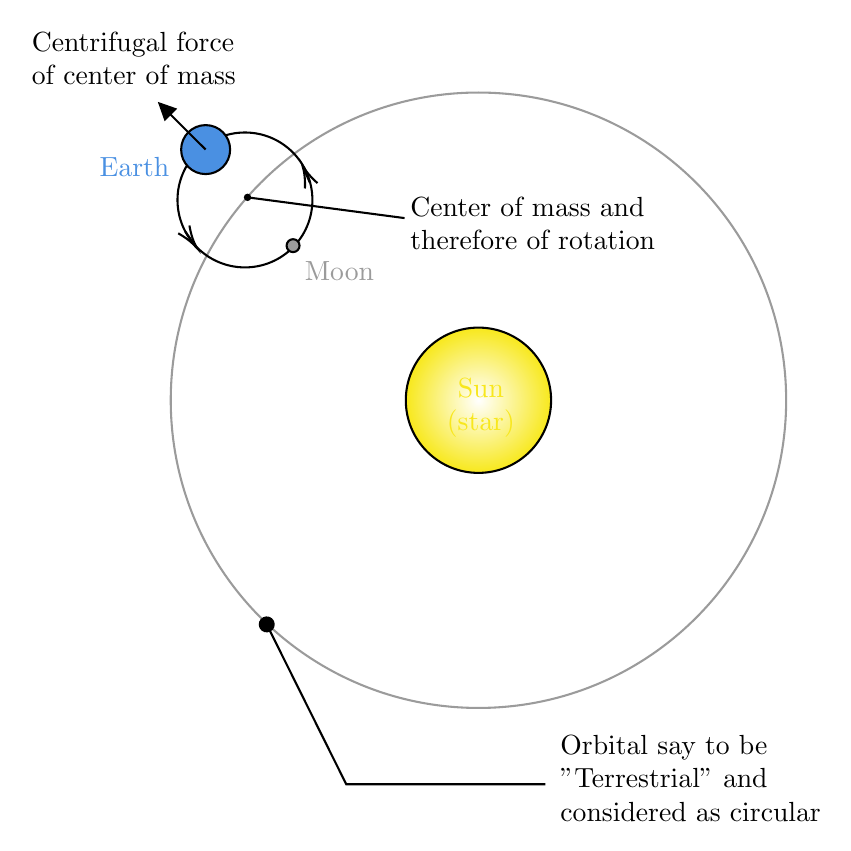
\begin{tikzpicture}[x=0.75pt,y=0.75pt,yscale=-1,xscale=1]
		%uncomment if require: \path (0,592); %set diagram left start at 0, and has height of 592
		
		% Gradient Info
  
		\tikzset {_thiir55cc/.code = {\pgfsetadditionalshadetransform{ \pgftransformshift{\pgfpoint{0 bp } { 0 bp }  }  \pgftransformscale{1 }  }}}
		\pgfdeclareradialshading{_5muc2o8in}{\pgfpoint{0bp}{0bp}}{rgb(0bp)=(1,1,1);
		rgb(0bp)=(1,1,1);
		rgb(25bp)=(0.97,0.91,0.11);
		rgb(400bp)=(0.97,0.91,0.11)}
		
		%Shape: Circle [id:dp10895971330282683] 
		\path  [shading=_5muc2o8in,_thiir55cc] (269,197) .. controls (269,177.67) and (284.67,162) .. (304,162) .. controls (323.33,162) and (339,177.67) .. (339,197) .. controls (339,216.33) and (323.33,232) .. (304,232) .. controls (284.67,232) and (269,216.33) .. (269,197) -- cycle ; % for fading 
		 \draw   (269,197) .. controls (269,177.67) and (284.67,162) .. (304,162) .. controls (323.33,162) and (339,177.67) .. (339,197) .. controls (339,216.33) and (323.33,232) .. (304,232) .. controls (284.67,232) and (269,216.33) .. (269,197) -- cycle ; % for border 
		
		%Shape: Circle [id:dp968410266404276] 
		\draw  [color={rgb, 255:red, 155; green, 155; blue, 155 }  ,draw opacity=1 ] (155.75,197) .. controls (155.75,115.12) and (222.12,48.75) .. (304,48.75) .. controls (385.88,48.75) and (452.25,115.12) .. (452.25,197) .. controls (452.25,278.88) and (385.88,345.25) .. (304,345.25) .. controls (222.12,345.25) and (155.75,278.88) .. (155.75,197) -- cycle ;
		%Straight Lines [id:da08776932869334586] 
		\draw    (202,305) -- (240.3,382) -- (336.3,382) ;
		\draw [shift={(202,305)}, rotate = 63.55] [color={rgb, 255:red, 0; green, 0; blue, 0 }  ][fill={rgb, 255:red, 0; green, 0; blue, 0 }  ][line width=0.75]      (0, 0) circle [x radius= 3.35, y radius= 3.35]   ;
		%Shape: Circle [id:dp5907832207752344] 
		\draw  [fill={rgb, 255:red, 0; green, 0; blue, 0 }  ,fill opacity=1 ] (191.5,99.25) .. controls (191.5,98.56) and (192.06,98) .. (192.75,98) .. controls (193.44,98) and (194,98.56) .. (194,99.25) .. controls (194,99.94) and (193.44,100.5) .. (192.75,100.5) .. controls (192.06,100.5) and (191.5,99.94) .. (191.5,99.25) -- cycle ;
		%Shape: Circle [id:dp07297756168153757] 
		\draw   (159,100.5) .. controls (159,82.55) and (173.55,68) .. (191.5,68) .. controls (209.45,68) and (224,82.55) .. (224,100.5) .. controls (224,118.45) and (209.45,133) .. (191.5,133) .. controls (173.55,133) and (159,118.45) .. (159,100.5) -- cycle ;
		%Straight Lines [id:da6463438389106655] 
		\draw    (162.72,115.64) -- (167.17,122) ;
		\draw [shift={(168.32,123.64)}, rotate = 235.01] [color={rgb, 255:red, 0; green, 0; blue, 0 }  ][line width=0.75]    (10.93,-3.29) .. controls (6.95,-1.4) and (3.31,-0.3) .. (0,0) .. controls (3.31,0.3) and (6.95,1.4) .. (10.93,3.29)   ;
		%Straight Lines [id:da4615688758020835] 
		\draw    (222.72,92.04) -- (219.91,85.48) ;
		\draw [shift={(219.12,83.64)}, rotate = 66.8] [color={rgb, 255:red, 0; green, 0; blue, 0 }  ][line width=0.75]    (10.93,-3.29) .. controls (6.95,-1.4) and (3.31,-0.3) .. (0,0) .. controls (3.31,0.3) and (6.95,1.4) .. (10.93,3.29)   ;
		%Shape: Circle [id:dp0003319738446478926] 
		\draw  [fill={rgb, 255:red, 155; green, 155; blue, 155 }  ,fill opacity=1 ] (211.56,122.52) .. controls (211.56,120.8) and (212.96,119.4) .. (214.68,119.4) .. controls (216.4,119.4) and (217.8,120.8) .. (217.8,122.52) .. controls (217.8,124.24) and (216.4,125.64) .. (214.68,125.64) .. controls (212.96,125.64) and (211.56,124.24) .. (211.56,122.52) -- cycle ;
		%Shape: Circle [id:dp12621351381355939] 
		\draw  [fill={rgb, 255:red, 74; green, 144; blue, 226 }  ,fill opacity=1 ] (160.76,76.24) .. controls (160.76,69.72) and (166.04,64.44) .. (172.56,64.44) .. controls (179.08,64.44) and (184.36,69.72) .. (184.36,76.24) .. controls (184.36,82.76) and (179.08,88.04) .. (172.56,88.04) .. controls (166.04,88.04) and (160.76,82.76) .. (160.76,76.24) -- cycle ;
		%Straight Lines [id:da7511704931791947] 
		\draw    (172.56,76.24) -- (151.64,55.36) ;
		\draw [shift={(149.52,53.24)}, rotate = 44.95] [fill={rgb, 255:red, 0; green, 0; blue, 0 }  ][line width=0.08]  [draw opacity=0] (8.93,-4.29) -- (0,0) -- (8.93,4.29) -- cycle    ;
		%Straight Lines [id:da8463349739290669] 
		\draw    (192.75,99.25) -- (268.4,109.24) ;
		
		% Text Node
		\draw (286,185) node [anchor=north west][inner sep=0.75pt]  [color={rgb, 255:red, 248; green, 231; blue, 28 }  ,opacity=1 ] [align=left] {\begin{minipage}[lt]{26.52pt}\setlength\topsep{0pt}
		\begin{center}
		Sun\\(star)
		\end{center}
		
		\end{minipage}};
		% Text Node
		\draw (342,357) node [anchor=north west][inner sep=0.75pt]   [align=left] {Orbital say to be\\"Terrestrial" and\\considered as circular};
		% Text Node
		\draw (87.32,18) node [anchor=north west][inner sep=0.75pt]   [align=left] {Centrifugal force\\of center of mass};
		% Text Node
		\draw (269.72,97.8) node [anchor=north west][inner sep=0.75pt]   [align=left] {Center of mass and\\therefore of rotation};
		% Text Node
		\draw (216.68,128.64) node [anchor=north west][inner sep=0.75pt]  [color={rgb, 255:red, 155; green, 155; blue, 155 }  ,opacity=1 ] [align=left] {\begin{minipage}[lt]{28.24pt}\setlength\topsep{0pt}
		\begin{center}
		Moon
		\end{center}
		
		\end{minipage}};
		% Text Node
		\draw (118.68,78.64) node [anchor=north west][inner sep=0.75pt]  [color={rgb, 255:red, 74; green, 144; blue, 226 }  ,opacity=1 ] [align=left] {\begin{minipage}[lt]{27.11pt}\setlength\topsep{0pt}
		\begin{center}
		Earth
		\end{center}
		
		\end{minipage}};
		
		\end{tikzpicture}
		\vspace*{3mm}
		\caption{Principle of tides superimposed on diurnal tides}
	\end{figure}
	And we will ignore the tides of equinoxes and others... at least for now...
	
	\pagebreak
	\subsection{Lorenz equations}\label{lorenz equations}
	The "\NewTerm{free convection}\index{free convection}" or "\NewTerm{natural convection}\index{natural convection}" is the flow regime obtained when we heat a fluid without imposing any external flow. This is the case for atmospheric convection movements (hot gases in cold gases), convection movements of the molten rock responsible for plate tectonics, movements of hot water under pressure in geysers or cakes... and many other phenomena...

	These flows are inexplicable if we do not couple the equations of dynamics and thermodynamics!

	We will in this context establish the famous system of Lorenz equations at the price, however, of numerous approximations and assumptions in order to simplify as much as possible the calculations and the mathematical tools used (because at the time of the development of the model the computers were not what they are today).

	We will therefore prove in the context of convection (one of the important dynamics of our atmosphere) that the equations which determine certain parameters of the motion are very sensitive to the initial conditions, the purpose of which is to show the difficulty of predicting to a more or less long term with deterministic theoretical models (reason why in meteorology we use nowadays the method of the finite elements).

	A priori, the density $\rho$ is a function of temperature and pressure by the state law of ideal gases (\SeeChapter{see section Continuum Mechanics page \pageref{ideal gas law}}). It is therefore natural to think that if we heat a wall, the temperature of the surrounding fluid increases by diffusion. The pressure stratification is changed, the pressure gradient creates the movement.
	\begin{figure}[H]
		\centering
		\includegraphics[scale=0.5]{img/engineering/free_convection.jpg}
		\caption{One of the everyday life most known convection...}
	\end{figure}
	In all sections of this book, we have so far neglected any variation of $\rho$. But decoupling is no longer valid here since it is heating that causes movement. We will therefore allow a variation of the density with the heating assuming however that this perturbation is small. It is therefore necessary to reintroduce a variation of $\rho$ around an equilibrium position: rest. On the other hand, the viscosity will be assumed constant...

	Thus, given a far fluid at rest and at the temperature $T_{\infty}$, it is in the presence of a wall heated to the temperature $T_P$. To obtain the dependence of $\rho$, let us recall some classical thermo-elastic coefficients (\SeeChapter{see section Thermodynamics page \pageref{thermo-elastic}}):
	\begin{itemize}
		\item Coefficient of isobaric compressibility (or dilatation according to the writing in terms of density):
		

		\item Isothermal compressibility coefficient:
		
	\end{itemize}
	By assuming now that density is mainly related to temperature (for simplicity) we can write (this hypothesis works well for fluids but not too much ... for gas !!):
	
	Using the general form of Taylor's development (\SeeChapter{see section Sequences and Series page \pageref{taylor series}}):
	
	We then have an approach with the engineer way... :
	
	Therefore:
	
	where $\bar{T}$ is therefore a coefficient without dimensions (as $\varepsilon$ ...) more easily measurable experimentally.

	The continuity equation (\SeeChapter{see section Thermodynamics page \pageref{continuity equation}}) or of mass balance that is for recall:
	
	Then becomes:
	
	to the first order in $\varepsilon$. Moreover, we have proved in the section of Continuum Mechanics (see page \pageref{incompressible flow}) that if the fluid is incompressible:
	
	Let us remember that in a first approximation the fluid is incompressible. It then only remains:
	
	As we wish to study a flow in the presence of gravity, it would be judicious to put:
	
	and therefore to focus only on variations around the hydrostatic equilibrium position ($\delta p$ is dimensionless!). We have proved still in the same section of Continuum Mechanics (see page \pageref{Euler equation of the 1st form}) that in the case of the incompressible fluid with viscosity, the first form of Euler's equation (equation of motion):
	
	Let us first consider the both terms:
	
	which are written along the $Z$ axis:
	
	When there is movement, the projection along $Z$ thus make appears:
	
	which we then rewrite:
	
	Therefore:
	
	since:
	
	It comes:
	
	It remains therefore a buoyancy force directed upward.

	The variation of the density as a function of temperature in the product $\rho\mathrm{d}_t\vec{v}$ of the relation:
	
	will be neglected ($\rho\mathrm{d}_t\vec{v}\cong \rho_\infty \mathrm{d}_t\vec{v}$) because we will restrict ourselves in case where the speed is small. We have then by reintroducing the viscosity...:
	
	and we have then material derivative (\SeeChapter{see section Continuum Mechanics page \pageref{material derivative}}):
	
	that we can simplify as:
	
	We then have as expression of the force density:
	
	To continue, we will seek to determine the energy law of the equation of behaviour proved in the section Continuum Mechanics (see page \pageref{general dynamic equation of stresses}) that was for recall:
	
	so that it also accounts for the relation between the stresses and thermodynamic characteristics of the fluid, such as heat flow and temperature. We will do this by characterizing the diffusion of energy in the medium due to the effects  (supposedly decoupled) of the viscosity of the fluid and the thermal conduction of the fluid.

	We rewrite this relation with new constants and another notation for the divergence:
	
	where $\mu_d$ and $\lambda$ are in this context named the "\NewTerm{Lamé coefficients}\index{Lamé coefficients}" (also named the "\NewTerm{Lamé parameters}\index{Lamé parameters}" or "\NewTerm{Lamé constants}\index{Lamé constants}"). The terms $\lambda$ and $\mu$ are individually referred to as "\NewTerm{Lamé's first parameter}" and "\NewTerm{Lamé's second parameter}".
	
	We have also proved in the section of Continuum Mechanics (see page \pageref{speed to stress relation}) the relation:
	
	Therefore:
	
	Which gives:
	
	Let us denote the total energy as:
	
	where $e$ is the internal mass energy of the fluid (so related to a unit of fluid mass). Now the instantaneous variation of the internal energy of the fluid is equal to the contribution of a mechanical power and of the supply of heat (according to what has been seen in the section of Thermodynamics):
	
	where $P$ gives the power of the external forces  to the system given necessarily by the force of the ambient potential field and the mechanical forces given by the stress tensor only (we are always in the situation of a perfect fluid). That is:
	
	and using the Ostrogradsky theorem (\SeeChapter{see section Vector Calculus page \pageref{gauss ostrogradsky theorem}}):
	
	which has indeed the units of a power. We also have:
	
	For the heat power $\dot{Q}$ it is very easy also thanks to the developments we had made in the section of Thermodynamics where we obtained the equation of heat (see page \pageref{heat equation}):
	
	Therefore:
	
	We have finally:
	
	So all this gives us the equation of the energy of a fluid:
	
	Therefore:
	
	and as (\SeeChapter{see section Thermodynamics page \pageref{fourier law}}) the heat flow follows the Fourier law:
	
	We have then:
	
	Either by using the Laplacian definition of a scalar field (\SeeChapter{see section Vector Calculus page \pageref{scalar laplacian}}):
	
	Or explicitly:
	
	Now, by making the scalar product of:
	
	With the velocity $\vec{v}$ we get the balance of the kinetic energy:
	
	That is to say explicitly:
	
	By subtracting (just proved earlier): 
	
	and (just proved also earlier above):
	
	we get a local relation of the specific internal energy $e$:
	
	That is to say explicitly:
	
	But we also have (derivation of a product):
	
	Therefore:
	
	Indeed:
	
	We have therefore:
	
	And as the stress tensor $\sigma$ is symmetric:
	
	we have therefore:
	
	which is sometimes written (yes I also don't believe what I see sometimes...):
	
	where $\overline{\overline{D}}$ is named the "\NewTerm{tensor of deformation rate}\index{tensor of deformation rate}" and $\overline{\overline{\sigma}} : \overline{\overline{D}}$ represents the double contracted product of the stress tensor and deformation rate tensor.

	We have proved, for recall, in the section of Continuum Mechanics (see page \pageref{general dynamic equation of stresses}) that:
	
	where:
	
	Therefore, it is simple to make the difference between normal forces and tangential forces. Whatever, to come back on the energy equation:
	
	and replacing explicitly the stress tensor $\sigma$, we get:
	
	But in our case:
	
	therefore we can write:
	
	But we also have (using the trace as seen in the section of Linear Algebra at page \pageref{trace of a matrix}):
	
	We have therefore:
	
	Thus into technical condensed form (just for information...):
	
	It is clear that from the point of view of the entropy (\SeeChapter{see section Thermodynamics page \pageref{entropy}}) we have:
	
	We also have:
	
	Thus reduced to the massic values:
	
	The time variation giving:
	
	But with have the continuity equation (\SeeChapter{see section Thermodynamics page \pageref{continuity equation}}):
	
	Which gives finally:
	
	or written slightly differently:
	
	Injected in:
	
	This gives:
	
	If we consider the velocity gradient to be very small (quasi-static) then we can write the approximation:
	
	Let us now give the expression of the entropy (exact total differential) as a function of the temperature and pressure parameters only:
	
	Either in massic form:
	
	But we have also proved in the section Thermodynamics (see page \pageref{Legendre transformation}) the following relation:
	
	Either in massic form:
	
	Which gives us:
	
	But, we have also proved in the section Thermodynamics (see page \pageref{Maxwell relations}), one of the following Maxwell's relations:
	
	Either in massic form:
	
	hence:
	
	Therefore:
	
	Then our relation:
	
	can be written:
	
	If we assume that the variation of the density with the temperature is small, we then have at the atmospheric scale:
	
	and remembering that (material derivative):
	
	It finally comes:
	
	We now have two important equations:
	
	Therefore:
	
	
	\subsubsection{Rayleigh-Bénard convection cells (Benard-Marangoni instability)}\label{convection cells}
	Let us now briefly examine the Rayleigh-Bénard\index{Rayleigh-Bénard convection cells} problem, which consists of two plates limiting one fluid being more heated than the other.
	\begin{tcolorbox}[title=Remark,arc=10pt,breakable,drop lifted shadow,
  skin=enhanced,
  skin first is subskin of={enhancedfirst}{arc=10pt,no shadow},
  skin middle is subskin of={enhancedmiddle}{arc=10pt,no shadow},
  skin last is subskin of={enhancedlast}{drop lifted shadow}]
	The "\NewTerm{Bénard-Marangoni instability}\index{Bénard-Marangoni instability}" is a free surface configuration of Rayleigh-Bénard instability. In fact, a thin layer of fluid is placed on a horizontal plane but its upper face is not in contact with an other plane but it is a free surface in contact with the air. The temperature of the lower plane must be superior to the temperature of the air to develop instabilities.
	\end{tcolorbox}
	We can then observe parallel longitudinal rolls in a film of viscous fluid (silicone oil) held between two plates at a hot temperature at the bottom and cold at the top. Here is a picture of these rolls seen from sides (but normally we don't notice it, because they only get visible when you add mark-particles):
	\begin{figure}[H]
		\centering
		\includegraphics[scale=1]{img/engineering/rayleigh_benard_convection_cell_oil_slice.jpg}	
		\caption{Rayleigh-Bénard convection cells (instability)}
	\end{figure}
	view from the top:
	\begin{figure}[H]
		\centering
		\includegraphics[scale=1]{img/engineering/rayleigh_benard_convection_cell_oil_from_top.jpg}	
		\caption{Rayleigh-Bénard convection cells viewed from top (instability)}
	\end{figure}
	It is a problem of natural convection: the heated fluid at the bottom expands and ascends entrained by the Archimedes principle, arrived at the top it cools and falls down. It is this movement that must be explained that is similar to that of the Earth's atmosphere, Sun convection cells and also Earth's mantel dynamics as illustrated below:
	\begin{figure}[H]
		\centering
		\includegraphics[scale=0.65]{img/engineering/rayleigh_benard_convection_cell_sun.jpg}	
		\caption[Rayleigh-Bénard convection cells on our Sun]{Rayleigh-Bénard convection cells on our Sun\index{solar granulation} (source: Swedish Vacuum Solar Telescope 11997-07-10)}
	\end{figure}
	\begin{figure}[H]
		\centering
		\includegraphics[scale=0.55]{img/engineering/rayleigh_benard_convection_cell_earth.jpg}	
		\caption[Rayleigh-Bénard convection cells on Earth]{Rayleigh-Bénard convection cells on Earth (source: ?)}
	\end{figure}
	\begin{figure}[H]
		\centering
		\includegraphics[scale=1]{img/engineering/rayleigh_benard_convection_cell_earth_mantle.jpg}	
		\caption[Rayleigh-Bénard convection cells as supposed in Earth mantle]{Rayleigh-Bénard convection cells as supposed in Earth mantle (source: ?)}
	\end{figure}
	We also notice experimentally that the convection movements are made approximately according to a torus (see the photo seen from the side just above). We can take advantage of this symmetry to simplify the analysis.
	
	Let us consider then a vertical loop of fluid circulating at constant speed (thus without too much turbulence ...):
	\begin{figure}[H]
		\centering
		
		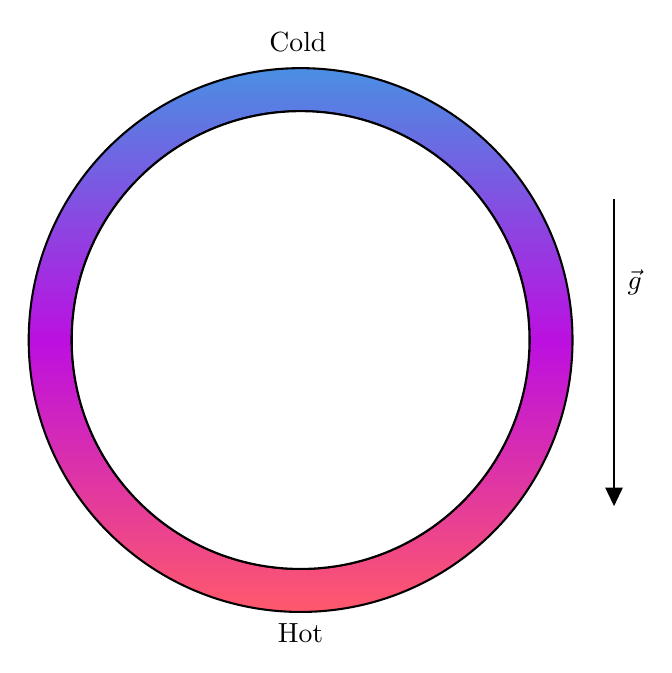
\begin{tikzpicture}[x=0.75pt,y=0.75pt,yscale=-1,xscale=1]
		%uncomment if require: \path (0,638); %set diagram left start at 0, and has height of 638
		
		% Gradient Info
		\tikzset {_zc2nyj7ko/.code = {\pgfsetadditionalshadetransform{ \pgftransformshift{\pgfpoint{0 bp } { 0 bp }  }  \pgftransformrotate{-90 }  \pgftransformscale{2 }  }}}
		\pgfdeclarehorizontalshading{_drq4g2zuv}{150bp}{rgb(0bp)=(0.29,0.56,0.89);
		rgb(37.5bp)=(0.29,0.56,0.89);
		rgb(50.089285714285715bp)=(0.74,0.06,0.88);
		rgb(62.5bp)=(1,0.35,0.42);
		rgb(100bp)=(1,0.35,0.42)}
		
		%Shape: Donut [id:dp9234474454127259] 
		\path  [shading=_drq4g2zuv,_zc2nyj7ko] (198.72,195) .. controls (198.72,134.09) and (248.09,84.72) .. (309,84.72) .. controls (369.91,84.72) and (419.28,134.09) .. (419.28,195) .. controls (419.28,255.91) and (369.91,305.28) .. (309,305.28) .. controls (248.09,305.28) and (198.72,255.91) .. (198.72,195)(178,195) .. controls (178,122.65) and (236.65,64) .. (309,64) .. controls (381.35,64) and (440,122.65) .. (440,195) .. controls (440,267.35) and (381.35,326) .. (309,326) .. controls (236.65,326) and (178,267.35) .. (178,195) ; % for fading 
		 \draw   (198.72,195) .. controls (198.72,134.09) and (248.09,84.72) .. (309,84.72) .. controls (369.91,84.72) and (419.28,134.09) .. (419.28,195) .. controls (419.28,255.91) and (369.91,305.28) .. (309,305.28) .. controls (248.09,305.28) and (198.72,255.91) .. (198.72,195)(178,195) .. controls (178,122.65) and (236.65,64) .. (309,64) .. controls (381.35,64) and (440,122.65) .. (440,195) .. controls (440,267.35) and (381.35,326) .. (309,326) .. controls (236.65,326) and (178,267.35) .. (178,195) ; % for border 
		
		%Shape: Circle [id:dp48875488545906287] 
		\draw  [fill={rgb, 255:red, 255; green, 255; blue, 255 }  ,fill opacity=1 ] (198.72,195) .. controls (198.72,134.09) and (248.09,84.72) .. (309,84.72) .. controls (369.91,84.72) and (419.28,134.09) .. (419.28,195) .. controls (419.28,255.91) and (369.91,305.28) .. (309,305.28) .. controls (248.09,305.28) and (198.72,255.91) .. (198.72,195) -- cycle ;
		%Straight Lines [id:da62193683580771] 
		\draw    (460,127) -- (460,272) ;
		\draw [shift={(460,275)}, rotate = 270] [fill={rgb, 255:red, 0; green, 0; blue, 0 }  ][line width=0.08]  [draw opacity=0] (8.93,-4.29) -- (0,0) -- (8.93,4.29) -- cycle    ;
		
		% Text Node
		\draw (465,159.4) node [anchor=north west][inner sep=0.75pt]    {$\vec{g}$};
		% Text Node
		\draw (292.5,45) node [anchor=north west][inner sep=0.75pt]   [align=left] {Cold};
		% Text Node
		\draw (296.5,330) node [anchor=north west][inner sep=0.75pt]   [align=left] {Hot};
		\end{tikzpicture}
		\vspace*{3mm}
		\caption{Vertical fluid loop with gradient in homogeneous gravific field}
	\end{figure}
	The configuration will be set as follows:
	\begin{figure}[H]
		\centering
		
		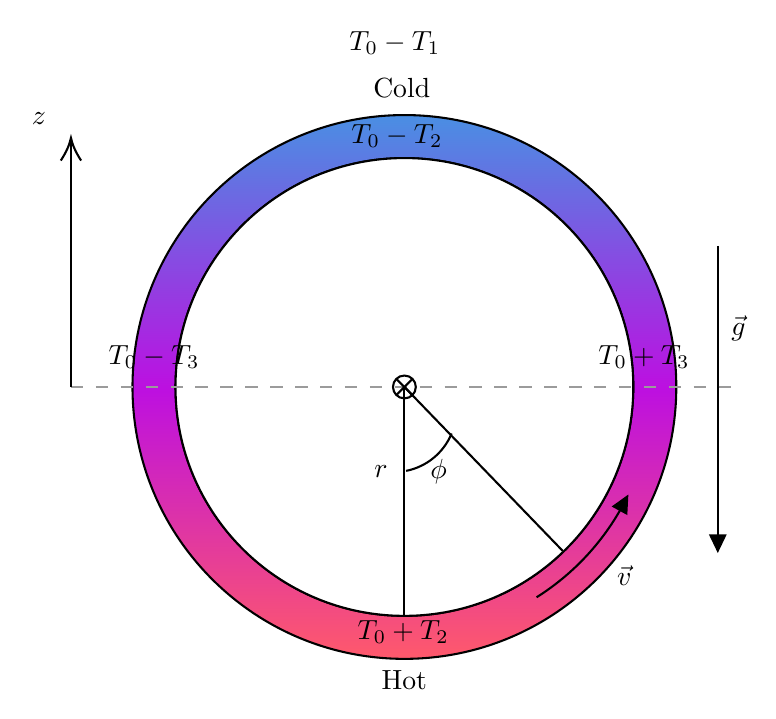
\begin{tikzpicture}[x=0.75pt,y=0.75pt,yscale=-1,xscale=1]
		%uncomment if require: \path (0,638); %set diagram left start at 0, and has height of 638
		% Gradient Info
		  
		\tikzset {_2liw759ep/.code = {\pgfsetadditionalshadetransform{ \pgftransformshift{\pgfpoint{0 bp } { 0 bp }  }  \pgftransformrotate{-90 }  \pgftransformscale{2 }  }}}
		\pgfdeclarehorizontalshading{_vjkkihmzc}{150bp}{rgb(0bp)=(0.29,0.56,0.89);
		rgb(37.5bp)=(0.29,0.56,0.89);
		rgb(50.089285714285715bp)=(0.74,0.06,0.88);
		rgb(62.5bp)=(1,0.35,0.42);
		rgb(100bp)=(1,0.35,0.42)}		
		%Shape: Donut [id:dp9234474454127259] 
		\path  [shading=_vjkkihmzc,_2liw759ep] (198.72,195) .. controls (198.72,134.09) and (248.09,84.72) .. (309,84.72) .. controls (369.91,84.72) and (419.28,134.09) .. (419.28,195) .. controls (419.28,255.91) and (369.91,305.28) .. (309,305.28) .. controls (248.09,305.28) and (198.72,255.91) .. (198.72,195)(178,195) .. controls (178,122.65) and (236.65,64) .. (309,64) .. controls (381.35,64) and (440,122.65) .. (440,195) .. controls (440,267.35) and (381.35,326) .. (309,326) .. controls (236.65,326) and (178,267.35) .. (178,195) ; % for fading 
		 \draw   (198.72,195) .. controls (198.72,134.09) and (248.09,84.72) .. (309,84.72) .. controls (369.91,84.72) and (419.28,134.09) .. (419.28,195) .. controls (419.28,255.91) and (369.91,305.28) .. (309,305.28) .. controls (248.09,305.28) and (198.72,255.91) .. (198.72,195)(178,195) .. controls (178,122.65) and (236.65,64) .. (309,64) .. controls (381.35,64) and (440,122.65) .. (440,195) .. controls (440,267.35) and (381.35,326) .. (309,326) .. controls (236.65,326) and (178,267.35) .. (178,195) ; % for border 
		
		%Shape: Circle [id:dp48875488545906287] 
		\draw  [fill={rgb, 255:red, 255; green, 255; blue, 255 }  ,fill opacity=1 ] (198.72,195) .. controls (198.72,134.09) and (248.09,84.72) .. (309,84.72) .. controls (369.91,84.72) and (419.28,134.09) .. (419.28,195) .. controls (419.28,255.91) and (369.91,305.28) .. (309,305.28) .. controls (248.09,305.28) and (198.72,255.91) .. (198.72,195) -- cycle ;
		%Straight Lines [id:da62193683580771] 
		\draw    (460,127) -- (460,272) ;
		\draw [shift={(460,275)}, rotate = 270] [fill={rgb, 255:red, 0; green, 0; blue, 0 }  ][line width=0.08]  [draw opacity=0] (8.93,-4.29) -- (0,0) -- (8.93,4.29) -- cycle    ;
		%Straight Lines [id:da6404702315964359] 
		\draw [color={rgb, 255:red, 155; green, 155; blue, 155 }  ,draw opacity=1 ] [dash pattern={on 4.5pt off 4.5pt}]  (148.35,195) -- (469.65,195) ;
		%Straight Lines [id:da8539317979069276] 
		\draw    (148.35,195) -- (148.35,77) ;
		\draw [shift={(148.35,75)}, rotate = 90] [color={rgb, 255:red, 0; green, 0; blue, 0 }  ][line width=0.75]    (10.93,-4.9) .. controls (6.95,-2.3) and (3.31,-0.67) .. (0,0) .. controls (3.31,0.67) and (6.95,2.3) .. (10.93,4.9)   ;
		%Shape: Arc [id:dp7675629449611234] 
		\draw  [draw opacity=0] (416.91,246.82) .. controls (407.1,267.19) and (391.7,284.36) .. (372.69,296.34) -- (309,195) -- cycle ; \draw    (415.55,249.55) .. controls (405.71,268.73) and (390.85,284.9) .. (372.69,296.34) ;  \draw [shift={(416.91,246.82)}, rotate = 118.62] [fill={rgb, 255:red, 0; green, 0; blue, 0 }  ][line width=0.08]  [draw opacity=0] (8.93,-4.29) -- (0,0) -- (8.93,4.29) -- cycle    ;
		%Straight Lines [id:da8864699862067071] 
		\draw    (309,195) -- (309,305.28) ;
		%Flowchart: Summing Junction [id:dp5566861915114987] 
		\draw   (303.5,195) .. controls (303.5,191.96) and (305.96,189.5) .. (309,189.5) .. controls (312.04,189.5) and (314.5,191.96) .. (314.5,195) .. controls (314.5,198.04) and (312.04,200.5) .. (309,200.5) .. controls (305.96,200.5) and (303.5,198.04) .. (303.5,195) -- cycle ; \draw   (305.11,191.11) -- (312.89,198.89) ; \draw   (312.89,191.11) -- (305.11,198.89) ;
		%Straight Lines [id:da5461158457957247] 
		\draw    (309,195) -- (385.3,274) ;
		%Shape: Arc [id:dp4942673976461187] 
		\draw  [draw opacity=0] (331.75,217.43) .. controls (327.95,226.66) and (319.71,233.48) .. (309.84,235.43) -- (304,206) -- cycle ; \draw   (331.75,217.43) .. controls (327.95,226.66) and (319.71,233.48) .. (309.84,235.43) ;  
		
		% Text Node
		\draw (465,159.4) node [anchor=north west][inner sep=0.75pt]    {$\vec{g}$};
		% Text Node
		\draw (292.5,45) node [anchor=north west][inner sep=0.75pt]   [align=left] {Cold};
		% Text Node
		\draw (296.5,330) node [anchor=north west][inner sep=0.75pt]   [align=left] {Hot};
		% Text Node
		\draw (281,22.4) node [anchor=north west][inner sep=0.75pt]    {$T_{0}-T_{1}$};
		% Text Node
		\draw (282,67) node [anchor=north west][inner sep=0.75pt]    {$T_{0}-T_{2}$};
		% Text Node
		\draw (285,306) node [anchor=north west][inner sep=0.75pt]    {$T_{0}+T_{2}$};
		% Text Node
		\draw (401,173.4) node [anchor=north west][inner sep=0.75pt]    {$T_{0}+T_{3}$};
		% Text Node
		\draw (165,173.4) node [anchor=north west][inner sep=0.75pt]    {$T_{0}-T_{3}$};
		% Text Node
		\draw (128,61.4) node [anchor=north west][inner sep=0.75pt]    {$z$};
		% Text Node
		\draw (410,279.4) node [anchor=north west][inner sep=0.75pt]    {$\vec{v}$};
		% Text Node
		\draw (293,231.4) node [anchor=north west][inner sep=0.75pt]    {$r$};
		% Text Node
		\draw (320,228.4) node [anchor=north west][inner sep=0.75pt]    {$\phi $};
		
		
		\end{tikzpicture}
		\vspace*{3mm}
		\caption{Required configuration for the theoretical model of convection cell}
	\end{figure}

	Where $T_0$ is the average temperature of the fluid (caution!: do not forget that it is not an extensive quantity!) and where we indicated respectively the temperatures inside the torus and outside it (i.e. the environment ) which may all vary with time.

	We see that the difference of temperature is of $2T_2$ between the top and the bottom and of $2T_3$ between the right and the left.

	We put that the temperature varies linearly with the height (which of course is false in an atmospheric model ...):
	
	We notice that it is possible to parametrise the temperature along the inside of the torus with the following relation (parametric equation of the circle):
	
	We have then according to the figure above:
	
	Having put this, let us return to:
	
	We will pass this system in polar coordinates best matching the geometry of our problem. Let us recall first that in term:
	
	the differential operator $\vec{\nabla}$ is the divergence. Now, we have proved in the section of Vector Calculus (see page \pageref{divergence in polar coordinates}) that this one was then written in polar coordinates:
	
	Now, if we rely on the hypothesis that in the volume of the torus the velocity varies neither as a function of the angle nor inside the torus (and therefore does not vary according to the radius $r$), then in polar coordinates :
	
	We have then:
	
	We will reduce the analysis to a single dimension which will be that the phenomenon depends only on the angle. We then have in polar coordinates and explicating all the terms:
	
	where we have at the same time made the projection along the $z$ axis such that:
	
	The differential coefficient of the last term will bother us. We replace it by a coefficient $\Gamma$ which we assume to be constant and which opposes the motion such as we have:
	
	or more explicitly:
	
	We now integrate this on the whole loop as a function of $\phi$. We have then:
	
	We then have the pressure term which disappears, because there is no pressure gradient along the loop. So:
	
	We then have for the first term (\SeeChapter{see section Differential and Integral Calculus page \pageref{usual primitives}}):
	
	and for the second term:
	
	Then it remains:
	
	Therefore:
	
	We see in this equation that the motion is driven by the horizontal temperature difference $T_3$.

	Now, let us come back to:
	
	If we neglect the tangential forces inside fluid, then we have:
	
	where $D$ is the thermal diffusion coefficient (\SeeChapter{see section Thermodynamics page \pageref{diffusion coefficient}}).

	In polar coordinates this is reduced to:
	
	and we will also make another approximation:
	
	And we have the two relations:
	
	By subtracting:
	
	Therefore:
	
	and also:
	
	Therefore:
	
	After derivation:
	
	We group together the terms:
	
	We then have the following three differential equations that govern the dynamics of the system:
	
	We finish the multiple simplifications by putting...:
	
	Which gives us:
	
	Putting it this in a more clean way, we get:
	
	Now, let introduce the following dimensionless variables:
	
	where we can assimilate:
	\begin{itemize}
		\item $X$ at the non-dimensional speed

		\item $Y$ to the non-dimensional temperature difference between rising and falling currents

		\item $Z$ to the dimensionless deviation of the convection equilibrium
	\end{itemize}
	We then have indeed:
	
	Therefore:
	
	In an even more condensed and traditional form:
	
	where we have:
	
	where we have:
	
	that correspond to the "\NewTerm{Prandtl number}\index{Prandlt number}" that a dimensionless number, named after the German physicist Ludwig Prandtl, defined as the ratio of "\NewTerm{momentum diffusivity}\index{momentum diffusivity}" to "\NewTerm{thermal diffusivity}\index{thermal diffusivity}" and where for recall:
	\begin{itemize}
		\item $\Gamma$ is the momentum diffusivity (kinematic viscosity) in $[\text{m}^2\cdot \text{s}^{-1}]$
		\item $K$ is the thermal diffusivity in $[\text{m}^2\cdot \text{s}^{-1}]$
		\item $\mu_d$ is the dynamic viscosity in $[\text{Ps}^2\cdot \text{s}]$
		\item $\kappa$ is the thermal conductivity in $[\text{W}\cdot \text{m}^{-1}\cdot\text{K}^{-1}]$
		\item $c_P$ is the specific heat in $[\text{J}\cdot\text{kg}^{-1}\cdot\text{K}^{-1}]$
	\end{itemize}
	with some typical values:
	\begin{table}[H]
		\centering
		\definecolor{gris}{gray}{0.85}
		\begin{tabular}{|l|c|}
			\hline
			{\cellcolor[gray]{0.75}\textbf{Material}} & {\cellcolor[gray]{0.75}\textbf{Prandtl Number Value}}  \\ \hline
			Molten potassium at $975$ [K] & $0.003$\\ \hline
			Mercury & $0.015$\\ \hline
			Noble gases & $0.16$-$0.17$ \\ \hline
			Oxygen & $0.63$ \\ \hline
			Molten lithium at $975$ [K] & $0.065$\\ \hline
			Air & $0.7$-$0.8$\\ \hline
			Gaseous ammoniac & $1.38$\\ \hline
			Water & $7$\\ \hline
			Seawater at $293$ [K] & $7.2$\\ \hline
			Seawater at $273$ [K] & $13.4$\\ \hline
			$n$-butanol & $50$\\ \hline
			Engine oil & $100$-$40,000$\\ \hline
			Glycerol & $1,000$\\ \hline
			Polymer melts & $10,000$\\ \hline
			Earth's mantle & $1\cdot 10^{25}$\\ \hline
		\end{tabular}
		\caption[Typical values for Pr]{Typical values for Pr (source: Wikipedia)}
	\end{table}
	And:
	
	which is assimilated to the "\NewTerm{Rayleigh number}\index{Rayleigh number}"  that is also a dimensionless number associated with "\NewTerm{buoyancy-driven flow}\index{buoyancy-driven flow}", also known as "\NewTerm{free convection}\index{free convection}" or "\NewTerm{natural convection}\index{natural convection}". When the Rayleigh number is below a critical value for that fluid, heat transfer is primarily in the form of conduction; when it exceeds the critical value, heat transfer is primarily in the form of convection.
	
	\subsubsection{Lorenz attractor and chaos}
	The previous system of three equations is essentially the same as that of the famous "\NewTerm{Lorenz system}\index{Lorenz system}". With one difference (!), the (real) Lorenz system contains a factor $b$ in the last equation (which does not change the result anyway since we still get a strange attractor in the end as we go on see):
	
	Pr, Re and $b$ are strictly positive, and we often put $\text{Pr}=10$, $\text{Re}=28$, $b=8/3$ where the Prandtl number corresponds to the value of that of water.

	The Lorenz equations describe the convection phenomena of an ideal two-dimensional fluid in a reservoir heated from below.

	We see by this by this proof that contrary to the statements not proved on many Internet pages and forums that:
	\begin{enumerate}
		\item The system is by no far not simple mathematically and is very approximate

		\item That there are simpler systems to study that are also chaotic (\SeeChapter{see section Population Dynamics page \pageref{chaotic logistic model}})
	\end{enumerate}
	The interest of the Lorenz equations lies, however, in the sensitivity to the initial conditions and the convergence of the dimensionless variables.

	Let's see an example with Maple 4.00b:

	\texttt{>with(DEtools):\\
		>lorenz:=diff(x(t),t) = 10*(y(t)-x(t)),diff(y(t),t) = 28*x(t)-y(t)-x(t)*z(t),\\
		diff(z(t),t) = x(t)*y(t)-8/3*z(t);\\
		>DEplot3d({lorenz}, [x(t),y(t),z(t)], t=0..100, stepsize=0.01, 
		[[x(0)=10, y(0)=10, z(0)=10]], orientation=[-35,75], linecolor = t, thickness = 1);\\
	}
	
	This gives for the first $100$ units of dimensionless time:
	\begin{figure}[H]
		\centering
		\includegraphics[scale=1]{img/engineering/lorenz_phase_system_maple.jpg}	
		\caption{Phase space of the Lorenz equations system in Maple 4.00b}
	\end{figure}
	or for the first $10$ units of dimensionless time:
	\begin{figure}[H]
		\centering
		\includegraphics[scale=1]{img/engineering/lorenz_phase_system_first_ten_time_units_maple.jpg}	
		\caption[]{Phase space of the Lorenz equations system in Maple 4.00b}
	\end{figure}
	Well so far we realize that the dimensionless parameters revolve around two points named the "\NewTerm{strange attractors}\index{strange attractors}".

	\textbf{Definition (\#\thesection.\mydef):} In the study of dynamic systems, an "\NewTerm{attractor}\index{attractor}" (or "\NewTerm{set-limit}\index{set-limit}") is a set, a curve or a space towards which a system evolves irreversibly in the absence of perturbations.

	Now always for the same values of adimensional time, we take $x(0)=10.1$, that is to say a relatively small change of the initial conditions. We have then:
	\begin{figure}[H]
		\centering
		\includegraphics[scale=1]{img/engineering/lorenz_phase_system_small_perturbation_maple.jpg}	
		\caption[]{Small variation in initial conditions of the Lorenz system with Maple 4.00b}
	\end{figure}
	We thus notice that the phenomenon is no longer really similar.

	Let us consider for example the variable $x$ taking as initial conditions:
	\begin{gather*}
		x(0)=10 \qquad y(0)=10 \qquad z(0)=10
	\end{gather*}
	then:
	\begin{gather*}
		x(0)=10 \qquad y(0)=10.1 \qquad z(0)=10
	\end{gather*}
	thus a small variation of $0.01$ on the value of $y(0)$.

	Either in Maple 4.00b:
	
	\texttt{>DEplot({lorenz}, [x(t), y(t), z(t)], t=0..15, stepsize = 0.01, [[x(0)=10, y(0)=10, z(0)=10],[x(0)=10, y(0)=10.01, z(0)=10]], scene = [t,x], linecolor = [blue,green], thickness = 1);}
	\begin{figure}[H]
		\centering
		\includegraphics[scale=1]{img/engineering/lorenz_phase_system_under_small_variation_of_initial_conditions_maple.jpg}	
		\caption[]{Analysis of the dimensionless variable $x$ for a small variation of initial conditions with Maple 4.00b}
	\end{figure}
	We see that the system shifts rather quickly from the initial model whereas at the beginning it remains identical but the overall shape remains.

	Another thing ... depending on the parameters the system can converge. Indeed, by changing the factor $28$ by the value $22$ we have for example (convergence on the left):
	\begin{figure}[H]
		\centering
		\includegraphics[scale=1]{img/engineering/lorenz_phase_system_convergence_maple.jpg}	
		\caption[]{Convergence of the Lorenz system with Maple 4.00b}
	\end{figure}
	or with the value $19$ the result is even more trivial:
	\begin{figure}[H]
		\centering
		\includegraphics[scale=1]{img/engineering/lorenz_phase_system_direct_convergence_maple.jpg}	
		\caption[]{Convergence of the Lorenz system with Maple 4.00b}
	\end{figure}
	Or with a value close to $1$:
	\begin{figure}[H]
		\centering
		\includegraphics[scale=1]{img/engineering/lorenz_phase_system_direct_fast_convergence_maple.jpg}	
		\caption[]{Fast convergence of the Lorenz system with Maple 4.00b}
	\end{figure}
	We notice a last interesting case is that if the Prandtl number is $1$ then the system is stable:
	\begin{figure}[H]
		\centering
		\includegraphics[scale=1]{img/engineering/lorenz_phase_system_stability_maple.jpg}	
		\caption[]{System Stability with Maple 4.00b}
	\end{figure}
	This sensitivity to the initial conditions, as well as the shape of the strange attractor of Lorenz, led the meteorologists to make a metaphor with the following sentence: can the flutter of a butterfly in Brazil cause a tornado in Texas?

	Hence the name afterwards of "\NewTerm{butterfly effect}\index{butterfly effect}" for the study of the attractor of Lorenz also named in the field the "\NewTerm{Lorenz's butterfly}\index{Lorenz's butterfly}".
	
	\pagebreak
	\subsection{Waves}\label{waves}
	When one finds himself on a boat, the movement of the water makes many people sick. It is also the case when one is in the galley to calculate this type of movement... Indeed, the waves in the water are neither transverse waves nor longitudinal waves. They are a bit of both. The water particles describe circles or ellipses, in a vertical plane parallel to the displacement of the wave. The big problem is that one of the boundary conditions is on the surface of the water and we do not know where that surface is. It is precisely one of the unknowns.
	\begin{figure}[H]
		\centering
		\includegraphics[width=0.7\textwidth]{img/engineering/waves.jpg}
	\end{figure}

	The problem is arduous enough for this calculation not to be found in books of general or specialized physics. We then tried to include it here by simplifying enormously and keeping only the simplest cases. The following calculation can be taken as an example of how physicists simplify life by making approximations and also as a masterful example of a common but complex phenomenon to be modelled.

	We will not compute the wave equation. We must calculate the motion of the particles from the surface to the bottom of the water, since the movement extends to the bottom. But since particles describe ellipses, we need at least two variables per point: we need a vector field! We will therefore calculate the vector field of the velocities of the particles, but we will not calculate it directly. What we will find is a scalar potential of velocities whose gradient will be the vector field of velocities.

	A final word on the waves that we will calculate. These waves are named "\NewTerm{gravity waves}\index{gravity names}" (not to be confused with "gravitational waves" in General Relativity), because it is the weight of the water that acts as a restoring force to bring down the summits and ascend the hollows.

	\begin{tcolorbox}[title=Remark,arc=10pt,breakable,drop lifted shadow,
  skin=enhanced,
  skin first is subskin of={enhancedfirst}{arc=10pt,no shadow},
  skin middle is subskin of={enhancedmiddle}{arc=10pt,no shadow},
  skin last is subskin of={enhancedlast}{drop lifted shadow}]
	I would like to thank Mr. Louis Peralta for his mathematical mastery and his pedagogy without which these exciting developments could never have been presented in this book. I am indebted to him, with his agreement, to copy / paste $99\%$ of his course material.
	\end{tcolorbox}
	

	We will make calculations in the simplest case: waves in a rectilinear channel of rectangular section and of constant width and depth... This reduces the dimensions of the problem to two (since the third one has an identical wave profile independently of where we are positioned in the width of the channel): the depth and direction of advance of the waves. Of course, we will neglect the friction on the bottom or sides of the canal and ... many other things.

	The coordinate system chosen is then:
	\begin{itemize}
		\item $x$ horizontal, positive in the direction of wave advancement (direction of channel length)

		\item $y$ horizontal in the direction perpendicular to the advancement of the waves (direction of the width of the channel). Again, no variable will depend on $y$ for the reasons already mentioned earlier

		\item $z$ vertical and positive upwards. The zero is chosen on the surface of undisturbed water. Under water, $z$ will therefore be negative. The depth of the channel being $h$, the bottom of the water will then be $z=-h$
	\end{itemize}
	Now, let us recall that we proved after very long developments in the section of Continuum Mechanics, that if the fluid is incompressible (divergence of the vector field of the velocities is therefore zero such that $\vec{\nabla}\circ\vec{v}=0$) and the dynamic viscosity is also ($\mu_d=0$), we then have the Euler equation of the first form (see page \pageref{Euler equation of the 1st form}):
	
	because $U$ is for recall of the scalar potential of the gravitational field.

	What we will explicitly write in the following form in the case of our study of gravity waves:
	
	Before continuing, we will change the form of the term $\mathrm{d}_t\vec{v}$ which is a total derivative and not partial. Let us consider one of the two components ($x$ or $z$) of this term. Let us take the component $x$ of the velocity vector and use what we saw in the section of Differential and Integral Calculus (we omitted the $y$ component since the system does not depend on it):
	
	We have in our situation:
	
	Then we get:
	
	The first term $\partial_t v_x$ is a linear term, whereas the other two are quadratic terms (as they include the product of a velocity by the derivative of a velocity) which are an infection (...) in all formal calculations. We shall therefore limit our calculations to cases where these quadratic terms are negligible relatively to the linear terms (implicitly implying that the speed must vary very little, otherwise this hypothesis is no longer valid). With this restriction, we then have:
	
	We can then write:
	
	We will add an additional restriction to our calculations. This restriction consists in imposing that the rotational velocity is zero:
	
	That is to say, as we have seen in the section of Continuum Mechanics, that there are no vortices in the fluid. We had already imposed that the velocity was zero in the $y$-direction, which prevents horizontal vortices horizontal axis of rotation). Now we eliminate the possibility of vortices with vertical axis of rotation also. It is not, in fact, too restrictive, we know that an object abandoned on the waves does not turn on itself unless it is caught in rolls. In the cases that we are going to calculate, the amplitudes are limited, we are in the linear case and, above all, not in the case of the rollers!!

	We have proved in the section of Vector Calculus that when the curl of a vector variable is zero, the variable can be expressed as the gradient of a scalar potential:
	
	It comes then that we can write:
	
	Then we get:
	
	What can be written:
	
	This equation acts as a wave equation, even if it does not directly describe the position or velocity of the particles. Once the equation of the function $\phi(x,z,t)$ are solved, we can deduce the velocities:
	
	It should not be forgotten that since the divergence of the vector field of the velocities is zero (incompressible field assumption):
	
	Therefore the scalar Laplacian of $\phi$ is zero:
	
	Therefore:
	
	with $-h<z<0$.
	
	The solution must satisfy boundary conditions. The most obvious is that the vertical velocity must be zero at the bottom of the water:
	
	To find the boundary conditions at the surface, we will define the variable $\xi(x,t)$ which is equal to the vertical displacement of a particle of water located on the surface of the water whose equilibrium position (in the absence of waves) is $x$ (not to be confused with the other $x$...!). The height of the surface of the water, measured by reference to the level of the water without wave, will therefore be given by $\xi(x,t)$. Thus, the vertical velocity $v_z$ at the surface of the water will be:
	
	This is a very subtle tip and not obvious at all to anticipate!

	At the surface, we can consider that the pressure $P$ is always equal to the atmospheric pressure for all the positions in $x$ and in $\xi$. Hence, a priori nothing will change if the atmospheric pressure changes (...), and it is more convenient to consider it null. With this, the equation:
	
	Becomes:
	
	From which we deduce:
	
	If we place ourselves on the surface, which corresponds to $z=0$, the preceding relation becomes:
	
	From which we deduce:
	
	If we place ourselves on the surface, which corresponds to $z=0$, the preceding relation becomes:
		
	and deriving this relation relatively to the time again, we get:
	
	Then using the relation proved just earlier above:
	
	It comes:
	
	Let us sum up the conditions that the scalar potential $\phi$ must satisfy:
	
	We will only look for solutions of the separable type (\SeeChapter{see section Differential and Integral Calculus page \pageref{separation vaiables method}}). That is to say that $\phi$, which is a function of $x$, $z$ and $t$, will then be able to be written as the product of three functions, each of which depends on a single variable. Moreover, we will work only in sinusoidal regime (an intuition ... of the observation in real life) and using the formalism of the phasors (\SeeChapter{see section Wave Mechanics page \pageref{phasors}}). Therefore, we have:
	
	As usual, we will only keep the real part of the phasors of the solutions at the end. 

	Let us now calculate the second partial derivatives with respect to $x$ and $z$:
		
	The following equation:
	
	tells us that under the surface, these two expressions are equal to a given sign:
	
	from which we deduce:
	
	$\lambda$ can only be a constant, since both sides of the expression depend on independent variables (which is very tricky for an observation!). This constant can take, in principle, any real or complex value.

	This gives us the following system of two independent differential equations of the second order:
	
	It is therefore a system of differential equations of order 2 independent, almost identical to that solved in the section of Thermodynamics when we studied the equation of heat.

	That being said, we do not know however the sign of the constant $\lambda$. What we know from what we have studied in the section of Differential and Integral Calculus is that if $b$ is positive then the solution of the differential equation in $z$:
	
	will have harmonic solutions. This would be very surprising ... and counter-intuitive with what we observe in reality. So we will impose $\lambda$ as being negative and then we have seen in the section of Differential and Integral Calculus that we will have by adopting pretty much the same notations:
	
	where we have the discriminant of the second differential equation (\SeeChapter{see section Differential and Integral Calculus page \pageref{second order differential equations}}) which holds:
	
	So in other words:
	
	It then comes:
	
	and the discriminant of the first differential equation will be purely complex:
	
	and therefore can be written:
	
	Our system is simplified even more:
	
	If we consider the advance as zero (null phase shift) we have:
	
	Since:	
	
	we have then:
	
	So in the second parenthesis, we just have two waves that go in opposite directions. Let's keep one of the two to simplify the analysis (no matter what!):
	
	To determine the constants, we will use the limit condition given above:
	
	Which in the present case gives us:
	
	So of course we are not going to simplify totally so that $k$ is zero otherwise it would not correspond with reality. On the other hand, we will simplify in the following way:
	
	Which imposes in the non-trivial case that:
	
	So we can choose what we want, but if we want to simplify life by anticipating what is coming ... it would be better to take the following choice:
	
	Therefore:
	
	Therefore we get:
	
	Using the hyperbolic functions (\SeeChapter{see section Trigonometry page \pageref{hyperbolic trigonometry}}) we have:
	
	We will continue to try to determine the constants using the second limit condition:
	
	Then it comes (for the derivative of the hyperbolic cosine see the section of Differential and Integral Calculus at page \pageref{usual derivatives}):
	
	and therefore by putting $z=0$:
	
	and simplifying:
	
	or written differently:
	
	Let us recall that (\SeeChapter{see section Wave Mechanics page \pageref{pulsation frequency period wave number}}):
	
	The prior-previous relation does not, to my knowledge, have any solution for expressing the phase velocity directly from an analytic expression (it is therefore transcendent) as a function of the depth $h$ and of the frequency $f$ (implicitly the pulsation $\omega$) of the wave without passing through a Maclaurin development (\SeeChapter{see section Sequences and Series page \pageref{usual maclaurin developments}}) of the hyperbolic tangent for small values of $kh$ such that:
	
	from which we derive when the depth $h$ and $k$ are also small by making an elementary simplification of the preceding relation:
	
	Relation which is named "\NewTerm{Lagrange celerity formula}\index{Lagrange celerity formula}". For example, for a tsunami, the wavelengths $\lambda$ are immense (on the order of a hundred kilometres) so the product $hk$ is small (of the order of $0.25$ in the oceans).

	If, on the other hand, the depth $h$ is very large as well as $k$ then we have in Taylor development  series (\SeeChapter{see section Sequences and Series page \pageref{usual maclaurin developments}}):
	
	from which we derive also after an elementary simplification:
	
	Relation which is named "\NewTerm{Newton celerity formula}\index{Newton celerity formula}".
	However we can numerically solve the relation:
	
	and then we have:
	\begin{figure}[H]
		\centering
		\includegraphics[scale=1]{img/engineering/gravity_wave_speed_period_plot.jpg}	
		\caption[Speed-Period gravity wave relation plot]{Speed-Period gravity wave relation plot (source: LPFR)}
	\end{figure}
	We can also by observing this plot understand why waves break (supercritical flux). Indeed, since the phase velocity for a given period increases as a function of the depth $h$, the upper part of the wave goes faster than the lower part and thus does not collapse due to lack of support. The supercritical part of the wave is destructive in the case of tsunamis because it is accelerated in its fall by gravity.

	It also follows that the larger waves catch up with the small ones and that their amplitudes are superimposed over a certain distance. We will determine later the function linking the amplitude of the wave to the distance.
	\begin{figure}[H]
		\centering
		\includegraphics[scale=1]{img/engineering/gravity_waves_type.jpg}	
		\caption[Most common type of well-known gravity wave]{Most common type of well-known gravity wave (source: ?)}
	\end{figure}
	Let us now return to:
	
	by conserving only the real part:
	
	Let us recall that we saw at the beginning:
	
	To get $Z$ we must therefore derive the prior-previous relation with respect to $z$ and then integrate the result with respect to time.

	The derivative thus gives:
	
	Therefore:
	
	The primitive gives:
	
	Therefore:
	
	And placing ourselves on $z=0$ (on the surface) we get:
	
	and by denoting by $R$ the amplitude of the wave:
	
	With this the vertical displacement $Z$ becomes:
	
	and remembering that the potential of speeds is given by:
	
	we can then rewrite it with this new constant $R$ as following:
	
	The horizontal velocity of a particle of water will then be:
	
	and the horizontal displacement will be the integral of the previous relation with respect to time:
	
	Therefore:
	
	and at the surface $z=0$:
	
	
	\subsubsection{Depth of a wave}
	It is now interesting to calculate the depth of penetration of the wave. Indeed, we know from experience that the waves are less and less visible as the water height is big (excepted for Rogue Wave that are special non-linear cases).

	Remember that we have just proved:
	
	Which corresponds to the vertical displacement of the wave. If:
	
	where we will consider that the wavelength of the waves is small and that the depth $h$ of the medium in which they propagate is large.

	We then have:
	
	and:
	
	and we see that for this approximation to be satisfied, it is necessary that:
	
	So that the remaining part of calculations to be valid, we will impose small values of $z$ (i.e. close to the surface).

	Since then:
	
	Without forgetting that $-h<z<0$ (so $z$ is negative for recall!). The amplitude of the movements thus decreases exponentially under these conditions with the depth. The reader can verify that for some values of small $kh$ we have:
	
	which shows the limitations of the model with this approach...
	
	\subsubsection{Wave's amplitude}
	For the amplitude of the horizontal movement the situation is the same. That is to say:
	
	where we will consider that the wavelength of the waves is small and that the depth $h$ of the medium in which they propagate is large.

	As we have proved earlier above that:
	
	It comes then:
	
	where for recall, we always have $-h<z<0$ and that this model is valid only near the surface.

	So for these two approximations, we have then when $z$ is small in absolute value with respect to $h$ (therefore in shallow water):
	
	Thus we can observe that for the case of equation and in shallow water (for $z$ small), the water particles describe a circular motion (since the two components $Z$ and $X$ have the same amplitude).

	On the other hand, in the general case, we have:
	
	The amplitudes are therefore no longer the same and the movements are then elliptic.
	\begin{figure}[H]
		\centering
		\includegraphics[scale=1]{img/engineering/gravity_wave_summary.jpg}	
		\caption[Water gravity wave study summary]{Water gravity wave study summary (source: ?)}
	\end{figure}

	\begin{flushright}
	\begin{tabular}{l c}
	\circled{70} & \pbox{20cm}{\score{2}{5} \\ {\tiny 30 votes,  48.00\%}} 
	\end{tabular} 
	\end{flushright}

	%to make section start on odd page
	\newpage
	\thispagestyle{empty}
	\mbox{}
	\section{Mechanical Engineering}\label{mechanical engineering}
	\lettrine[lines=4]{\color{BrickRed}M}{echanical Engineering}\index{mechanical engineering} is the set of knowledge related to mechanics, at the physical sense (sciences of movements) and at the technical sense (the study of mechanisms). This field of knowledge goes from design of mechanical product to the recycling of this latter through the way, of course, of production, maintenance, etc. Its applications are very important in many areas of everyday life either for the manufacture of machinery, toys, home appliances, medical devices or buildings or a variety of means of transport... and the list goes on...
	
	Again, we will focus here only on the mathematical formalization of practical cases of current applications in the industry! So this section is only a general introduction to technical applications of mechanics and must be complemented by laboratory practices (or computer simulation with for the SimuLink™ MATLAB™ toolbox and the SimDriveline™ MATLAB™ toolbox) and by reading also the section of Thermodynamics where the solid state equation is treated (see page \pageref{sate equation of solids}) and the section of Continuum Mechanics where the Navier-Stokes equation is proved (see page \pageref{navier stokes equations}). The mix of mechanics and magnetism systems (AC motors for example) is treated in the section of Electrodynmics (see page \pageref{electrodynamics}).
	
	\begin{tcolorbox}[title=Remark,arc=10pt,breakable,drop lifted shadow,
  skin=enhanced,
  skin first is subskin of={enhancedfirst}{arc=10pt,no shadow},
  skin middle is subskin of={enhancedmiddle}{arc=10pt,no shadow},
  skin last is subskin of={enhancedlast}{drop lifted shadow}]
	It would be pretentious to claim to do with this section as well and also as complete as two free French PDFs \textit{Éléments de machine} and \textit{Résistance des Matériaux} of Nicolet Gaston Raymond that are at our point of view unrivaled in content and quality at this date (compared to the same non-free books on the same subjects!). It is therefore strongly recommended to refer to them if you want to drive full information about mechanical engineering (see the download section of the companion website or directly his own website \url{http://www.raymondnicolet.ch}). Same recommendation applies to the reader about the master pieces that are the English books \textit{Mechanics of Materials} (\cite{hibbeler2011mechanics}) and \textit{Structural and Stress Analysis} (\cite{megson2005structural})!
	\end{tcolorbox}
	
	\subsection{Mechanical Efficiency}\label{mechanical efficiency}
	Mechanical advantage is a measure of the force amplification achieved by using a tool, mechanical device or machine system. The device preserves the input power and simply trades off forces against movement to obtain a desired amplification in the output force. Machine components designed to manage forces and movement in this way are named "mechanisms".
	
	Mechanical advantage that is computed using the assumption that no power is lost through deflection, friction and wear of a machine is the maximum performance that can be achieved. For this reason, it is often named the "\NewTerm{ideal mechanical advantage}\index{ideal mechanical advantage}" (IMA). In operation, deflection, friction and wear will reduce the mechanical advantage. The amount of this reduction from the ideal to the "\NewTerm{actual mechanical advantage}\index{actual mechanical advantage}" (AMA) is defined by a factor named "efficiency", a quantity which is determined by experimentation.

	The assumptions of an ideal machine are equivalent to the requirement that the machine does not store or dissipate energy; the power into the machine thus equals the power out. Therefore, the power $P$ is constant through the machine and force times velocity into the machine equals the force times velocity out, that is:
	
	The ideal mechanical advantage is the ratio of the force out of the machine (load) to the force into the machine (effort), or:
	
	Applying the constant power relationship yields a formula for this ideal mechanical advantage in terms of the speed ratio:
	
	The speed ratio of a machine can be calculated from its physical dimensions. The assumption of constant power thus allows use of the speed ratio to determine the maximum value for the mechanical advantage.
	\begin{figure}[H]
		\centering
		% Pattern Info
		 
		\tikzset{
		pattern size/.store in=\mcSize, 
		pattern size = 5pt,
		pattern thickness/.store in=\mcThickness, 
		pattern thickness = 0.3pt,
		pattern radius/.store in=\mcRadius, 
		pattern radius = 1pt}
		\makeatletter
		\pgfutil@ifundefined{pgf@pattern@name@_my28iakui}{
		\pgfdeclarepatternformonly[\mcThickness,\mcSize]{_my28iakui}
		{\pgfqpoint{0pt}{-\mcThickness}}
		{\pgfpoint{\mcSize}{\mcSize}}
		{\pgfpoint{\mcSize}{\mcSize}}
		{
		\pgfsetcolor{\tikz@pattern@color}
		\pgfsetlinewidth{\mcThickness}
		\pgfpathmoveto{\pgfqpoint{0pt}{\mcSize}}
		\pgfpathlineto{\pgfpoint{\mcSize+\mcThickness}{-\mcThickness}}
		\pgfusepath{stroke}
		}}
		\makeatother
		
		% Pattern Info
		 
		\tikzset{
		pattern size/.store in=\mcSize, 
		pattern size = 5pt,
		pattern thickness/.store in=\mcThickness, 
		pattern thickness = 0.3pt,
		pattern radius/.store in=\mcRadius, 
		pattern radius = 1pt}
		\makeatletter
		\pgfutil@ifundefined{pgf@pattern@name@_egklxgsva}{
		\pgfdeclarepatternformonly[\mcThickness,\mcSize]{_egklxgsva}
		{\pgfqpoint{0pt}{-\mcThickness}}
		{\pgfpoint{\mcSize}{\mcSize}}
		{\pgfpoint{\mcSize}{\mcSize}}
		{
		\pgfsetcolor{\tikz@pattern@color}
		\pgfsetlinewidth{\mcThickness}
		\pgfpathmoveto{\pgfqpoint{0pt}{\mcSize}}
		\pgfpathlineto{\pgfpoint{\mcSize+\mcThickness}{-\mcThickness}}
		\pgfusepath{stroke}
		}}
		\makeatother
		
		% Pattern Info
		 
		\tikzset{
		pattern size/.store in=\mcSize, 
		pattern size = 5pt,
		pattern thickness/.store in=\mcThickness, 
		pattern thickness = 0.3pt,
		pattern radius/.store in=\mcRadius, 
		pattern radius = 1pt}
		\makeatletter
		\pgfutil@ifundefined{pgf@pattern@name@_b28h0qx38}{
		\pgfdeclarepatternformonly[\mcThickness,\mcSize]{_b28h0qx38}
		{\pgfqpoint{0pt}{-\mcThickness}}
		{\pgfpoint{\mcSize}{\mcSize}}
		{\pgfpoint{\mcSize}{\mcSize}}
		{
		\pgfsetcolor{\tikz@pattern@color}
		\pgfsetlinewidth{\mcThickness}
		\pgfpathmoveto{\pgfqpoint{0pt}{\mcSize}}
		\pgfpathlineto{\pgfpoint{\mcSize+\mcThickness}{-\mcThickness}}
		\pgfusepath{stroke}
		}}
		\makeatother
		\tikzset{every picture/.style={line width=0.75pt}} %set default line width to 0.75pt        
		
		\begin{tikzpicture}[x=0.75pt,y=0.75pt,yscale=-1,xscale=1]
		%uncomment if require: \path (0,850); %set diagram left start at 0, and has height of 850
		
		%Shape: Rectangle [id:dp35532526757031335] 
		\draw  [fill={rgb, 255:red, 186; green, 183; blue, 183 }  ,fill opacity=1 ] (446.69,290.91) -- (459.19,290.91) -- (459.19,350.6) -- (446.69,350.6) -- cycle ;
		%Shape: Rectangle [id:dp21554811400403784] 
		\draw  [fill={rgb, 255:red, 186; green, 183; blue, 183 }  ,fill opacity=1 ] (466.07,285.91) -- (562.66,285.91) -- (562.66,289.6) -- (466.07,289.6) -- cycle ;
		%Straight Lines [id:da3485877703912854] 
		\draw [color={rgb, 255:red, 74; green, 144; blue, 226 }  ,draw opacity=1 ][line width=1.5]    (290.03,316.73) -- (303.54,340.26) ;
		\draw [shift={(305.53,343.73)}, rotate = 240.14] [fill={rgb, 255:red, 74; green, 144; blue, 226 }  ,fill opacity=1 ][line width=0.08]  [draw opacity=0] (10.45,-5.02) -- (0,0) -- (10.45,5.02) -- cycle    ;
		%Shape: Triangle [id:dp5658357342731237] 
		\draw  [fill={rgb, 255:red, 128; green, 128; blue, 128 }  ,fill opacity=1 ] (158.44,52.28) -- (165.88,63.28) -- (151,63.28) -- cycle ;
		%Shape: Rectangle [id:dp5838050727481803] 
		\draw  [fill={rgb, 255:red, 197; green, 194; blue, 194 }  ,fill opacity=1 ] (131,48) -- (248.88,48) -- (248.88,53.28) -- (131,53.28) -- cycle ;
		%Straight Lines [id:da10398352199430527] 
		\draw [color={rgb, 255:red, 208; green, 2; blue, 27 }  ,draw opacity=1 ][line width=1.5]    (131,19.28) -- (131,44) ;
		\draw [shift={(131,48)}, rotate = 270] [fill={rgb, 255:red, 208; green, 2; blue, 27 }  ,fill opacity=1 ][line width=0.08]  [draw opacity=0] (10.45,-5.02) -- (0,0) -- (10.45,5.02) -- cycle    ;
		%Straight Lines [id:da47126523827087685] 
		\draw [color={rgb, 255:red, 74; green, 144; blue, 226 }  ,draw opacity=1 ][line width=1.5]    (248.88,26.28) -- (248.88,44) ;
		\draw [shift={(248.88,48)}, rotate = 270] [fill={rgb, 255:red, 74; green, 144; blue, 226 }  ,fill opacity=1 ][line width=0.08]  [draw opacity=0] (10.45,-5.02) -- (0,0) -- (10.45,5.02) -- cycle    ;
		%Straight Lines [id:da6603432942997114] 
		\draw    (158.44,45.28) -- (158.44,30.28) ;
		%Straight Lines [id:da9462972673289844] 
		\draw    (136.88,38.28) -- (154.88,38.28) ;
		\draw [shift={(156.88,38.28)}, rotate = 180] [color={rgb, 255:red, 0; green, 0; blue, 0 }  ][line width=0.75]    (6.56,-1.97) .. controls (4.17,-0.84) and (1.99,-0.18) .. (0,0) .. controls (1.99,0.18) and (4.17,0.84) .. (6.56,1.97)   ;
		\draw [shift={(134.88,38.28)}, rotate = 0] [color={rgb, 255:red, 0; green, 0; blue, 0 }  ][line width=0.75]    (6.56,-1.97) .. controls (4.17,-0.84) and (1.99,-0.18) .. (0,0) .. controls (1.99,0.18) and (4.17,0.84) .. (6.56,1.97)   ;
		%Straight Lines [id:da9891992204402884] 
		\draw    (158.88,38.28) -- (246.88,38.28) ;
		\draw [shift={(248.88,38.28)}, rotate = 180] [color={rgb, 255:red, 0; green, 0; blue, 0 }  ][line width=0.75]    (6.56,-1.97) .. controls (4.17,-0.84) and (1.99,-0.18) .. (0,0) .. controls (1.99,0.18) and (4.17,0.84) .. (6.56,1.97)   ;
		\draw [shift={(156.88,38.28)}, rotate = 0] [color={rgb, 255:red, 0; green, 0; blue, 0 }  ][line width=0.75]    (6.56,-1.97) .. controls (4.17,-0.84) and (1.99,-0.18) .. (0,0) .. controls (1.99,0.18) and (4.17,0.84) .. (6.56,1.97)   ;
		%Shape: Right Triangle [id:dp740771322882785] 
		\draw  [fill={rgb, 255:red, 197; green, 194; blue, 194 }  ,fill opacity=1 ] (555.88,28.19) -- (370,95.19) -- (555.88,95.19) -- cycle ;
		%Shape: Rectangle [id:dp7968361161962445] 
		\draw  [fill={rgb, 255:red, 128; green, 128; blue, 128 }  ,fill opacity=1 ] (434.5,36.64) -- (488.87,16.19) -- (500.65,47.51) -- (446.28,67.95) -- cycle ;
		%Straight Lines [id:da6510250075547905] 
		\draw [color={rgb, 255:red, 208; green, 2; blue, 27 }  ,draw opacity=1 ][line width=1.5]    (410.88,65.19) -- (437.2,53.78) ;
		\draw [shift={(440.88,52.19)}, rotate = 156.57] [fill={rgb, 255:red, 208; green, 2; blue, 27 }  ,fill opacity=1 ][line width=0.08]  [draw opacity=0] (10.45,-5.02) -- (0,0) -- (10.45,5.02) -- cycle    ;
		%Shape: Circle [id:dp3551015190012088] 
		\draw  [fill={rgb, 255:red, 197; green, 194; blue, 194 }  ,fill opacity=1 ] (154.73,160.69) .. controls (154.73,134.45) and (175.99,113.19) .. (202.23,113.19) .. controls (228.46,113.19) and (249.73,134.45) .. (249.73,160.69) .. controls (249.73,186.92) and (228.46,208.19) .. (202.23,208.19) .. controls (175.99,208.19) and (154.73,186.92) .. (154.73,160.69) -- cycle ;
		%Shape: Circle [id:dp3738869127112434] 
		\draw  [fill={rgb, 255:red, 128; green, 128; blue, 128 }  ,fill opacity=1 ] (187.73,160.69) .. controls (187.73,152.68) and (194.22,146.19) .. (202.23,146.19) .. controls (210.24,146.19) and (216.73,152.68) .. (216.73,160.69) .. controls (216.73,168.7) and (210.24,175.19) .. (202.23,175.19) .. controls (194.22,175.19) and (187.73,168.7) .. (187.73,160.69) -- cycle ;
		%Straight Lines [id:da9891729177113351] 
		\draw    (202.73,160.69) -- (217.07,118.6) ;
		\draw [shift={(217.72,116.71)}, rotate = 108.82] [color={rgb, 255:red, 0; green, 0; blue, 0 }  ][line width=0.75]    (6.56,-1.97) .. controls (4.17,-0.84) and (1.99,-0.18) .. (0,0) .. controls (1.99,0.18) and (4.17,0.84) .. (6.56,1.97)   ;
		%Straight Lines [id:da6773743375316934] 
		\draw    (202.73,160.69) -- (191.52,166.09) ;
		\draw [shift={(189.72,166.96)}, rotate = 334.26] [color={rgb, 255:red, 0; green, 0; blue, 0 }  ][line width=0.75]    (6.56,-1.97) .. controls (4.17,-0.84) and (1.99,-0.18) .. (0,0) .. controls (1.99,0.18) and (4.17,0.84) .. (6.56,1.97)   ;
		%Straight Lines [id:da09802017874990443] 
		\draw [color={rgb, 255:red, 128; green, 128; blue, 128 }  ,draw opacity=1 ]   (187.73,160.69) -- (187.73,210.19) ;
		%Shape: Square [id:dp021301751784627898] 
		\draw  [fill={rgb, 255:red, 128; green, 128; blue, 128 }  ,fill opacity=1 ] (179.97,214.28) -- (194.88,214.28) -- (194.88,229.19) -- (179.97,229.19) -- cycle ;
		%Straight Lines [id:da3652243689513346] 
		\draw [color={rgb, 255:red, 74; green, 144; blue, 226 }  ,draw opacity=1 ][line width=1.5]    (239,130.28) -- (274.97,164.43) ;
		\draw [shift={(277.88,167.19)}, rotate = 223.51] [fill={rgb, 255:red, 74; green, 144; blue, 226 }  ,fill opacity=1 ][line width=0.08]  [draw opacity=0] (10.45,-5.02) -- (0,0) -- (10.45,5.02) -- cycle    ;
		%Shape: Circle [id:dp7249634572186059] 
		\draw   (155.23,160.69) .. controls (155.23,134.45) and (176.49,113.19) .. (202.73,113.19) .. controls (228.96,113.19) and (250.23,134.45) .. (250.23,160.69) .. controls (250.23,186.92) and (228.96,208.19) .. (202.73,208.19) .. controls (176.49,208.19) and (155.23,186.92) .. (155.23,160.69) -- cycle ;
		%Straight Lines [id:da8284902348641932] 
		\draw [color={rgb, 255:red, 208; green, 2; blue, 27 }  ,draw opacity=1 ][line width=1.5]    (187.42,221.73) -- (187.42,244.19) ;
		\draw [shift={(187.42,248.19)}, rotate = 270] [fill={rgb, 255:red, 208; green, 2; blue, 27 }  ,fill opacity=1 ][line width=0.08]  [draw opacity=0] (10.45,-5.02) -- (0,0) -- (10.45,5.02) -- cycle    ;
		%Shape: Triangle [id:dp9460816710362439] 
		\draw  [fill={rgb, 255:red, 128; green, 128; blue, 128 }  ,fill opacity=1 ] (406.81,181.46) -- (524.16,169.19) -- (523.88,196.19) -- cycle ;
		%Straight Lines [id:da2812232325020967] 
		\draw [color={rgb, 255:red, 74; green, 144; blue, 226 }  ,draw opacity=1 ][line width=1.5]    (559.88,185.19) -- (528.88,185.19) ;
		\draw [shift={(524.88,185.19)}, rotate = 360] [fill={rgb, 255:red, 74; green, 144; blue, 226 }  ,fill opacity=1 ][line width=0.08]  [draw opacity=0] (10.45,-5.02) -- (0,0) -- (10.45,5.02) -- cycle    ;
		%Straight Lines [id:da9166470381450378] 
		\draw    (409,176.19) -- (409,157.19) ;
		%Straight Lines [id:da20282418885860953] 
		\draw    (524,164.19) -- (524,157.19) ;
		%Straight Lines [id:da6020165120883543] 
		\draw    (411,161.19) -- (522,161.19) ;
		\draw [shift={(524,161.19)}, rotate = 180] [color={rgb, 255:red, 0; green, 0; blue, 0 }  ][line width=0.75]    (6.56,-1.97) .. controls (4.17,-0.84) and (1.99,-0.18) .. (0,0) .. controls (1.99,0.18) and (4.17,0.84) .. (6.56,1.97)   ;
		\draw [shift={(409,161.19)}, rotate = 0] [color={rgb, 255:red, 0; green, 0; blue, 0 }  ][line width=0.75]    (6.56,-1.97) .. controls (4.17,-0.84) and (1.99,-0.18) .. (0,0) .. controls (1.99,0.18) and (4.17,0.84) .. (6.56,1.97)   ;
		%Shape: Circle [id:dp5706599001396113] 
		\draw  [fill={rgb, 255:red, 128; green, 128; blue, 128 }  ,fill opacity=1 ] (130.73,312.69) .. controls (130.73,304.68) and (137.22,298.19) .. (145.23,298.19) .. controls (153.24,298.19) and (159.73,304.68) .. (159.73,312.69) .. controls (159.73,320.7) and (153.24,327.19) .. (145.23,327.19) .. controls (137.22,327.19) and (130.73,320.7) .. (130.73,312.69) -- cycle ;
		%Shape: Circle [id:dp36920260723679466] 
		\draw  [fill={rgb, 255:red, 128; green, 128; blue, 128 }  ,fill opacity=1 ] (194.73,332.69) .. controls (194.73,324.68) and (201.22,318.19) .. (209.23,318.19) .. controls (217.24,318.19) and (223.73,324.68) .. (223.73,332.69) .. controls (223.73,340.7) and (217.24,347.19) .. (209.23,347.19) .. controls (201.22,347.19) and (194.73,340.7) .. (194.73,332.69) -- cycle ;
		%Shape: Circle [id:dp19758176286530515] 
		\draw  [fill={rgb, 255:red, 128; green, 128; blue, 128 }  ,fill opacity=1 ] (269.23,319.69) .. controls (269.23,313.89) and (273.93,309.19) .. (279.73,309.19) .. controls (285.53,309.19) and (290.23,313.89) .. (290.23,319.69) .. controls (290.23,325.49) and (285.53,330.19) .. (279.73,330.19) .. controls (273.93,330.19) and (269.23,325.49) .. (269.23,319.69) -- cycle ;
		%Shape: Circle [id:dp1259981068444218] 
		\draw  [fill={rgb, 255:red, 128; green, 128; blue, 128 }  ,fill opacity=1 ] (274.23,339.69) .. controls (274.23,336.65) and (276.69,334.19) .. (279.73,334.19) .. controls (282.76,334.19) and (285.23,336.65) .. (285.23,339.69) .. controls (285.23,342.73) and (282.76,345.19) .. (279.73,345.19) .. controls (276.69,345.19) and (274.23,342.73) .. (274.23,339.69) -- cycle ;
		%Shape: Circle [id:dp8159314670855065] 
		\draw  [fill={rgb, 255:red, 128; green, 128; blue, 128 }  ,fill opacity=1 ] (274.23,372.69) .. controls (274.23,369.65) and (276.69,367.19) .. (279.73,367.19) .. controls (282.76,367.19) and (285.23,369.65) .. (285.23,372.69) .. controls (285.23,375.73) and (282.76,378.19) .. (279.73,378.19) .. controls (276.69,378.19) and (274.23,375.73) .. (274.23,372.69) -- cycle ;
		%Shape: Circle [id:dp15255255851567084] 
		\draw  [fill={rgb, 255:red, 128; green, 128; blue, 128 }  ,fill opacity=1 ] (269.23,393.69) .. controls (269.23,387.89) and (273.93,383.19) .. (279.73,383.19) .. controls (285.53,383.19) and (290.23,387.89) .. (290.23,393.69) .. controls (290.23,399.49) and (285.53,404.19) .. (279.73,404.19) .. controls (273.93,404.19) and (269.23,399.49) .. (269.23,393.69) -- cycle ;
		%Shape: Rectangle [id:dp14884769117084495] 
		\draw  [fill={rgb, 255:red, 206; green, 201; blue, 201 }  ,fill opacity=1 ] (142.46,291.55) -- (147.99,291.55) -- (147.99,315.23) -- (142.46,315.23) -- cycle ;
		%Shape: Rectangle [id:dp7462002236784755] 
		\draw  [fill={rgb, 255:red, 206; green, 201; blue, 201 }  ,fill opacity=1 ] (206.46,330.55) -- (211.99,330.55) -- (211.99,354.23) -- (206.46,354.23) -- cycle ;
		%Shape: Rectangle [id:dp17940564593259278] 
		\draw  [fill={rgb, 255:red, 206; green, 201; blue, 201 }  ,fill opacity=1 ] (276.96,304.05) -- (282.49,304.05) -- (282.49,349.23) -- (276.96,349.23) -- cycle ;
		%Shape: Rectangle [id:dp8405642788369398] 
		\draw  [fill={rgb, 255:red, 206; green, 201; blue, 201 }  ,fill opacity=1 ] (277.06,365.01) -- (282.39,365.01) -- (282.39,407.16) -- (277.06,407.16) -- cycle ;
		%Straight Lines [id:da9011764779148583] 
		\draw [line width=1.5]    (134.24,291.55) -- (155.74,291.55) ;
		%Straight Lines [id:da5555804105704625] 
		\draw [line width=1.5]    (186.24,304.55) -- (207.74,304.55) ;
		%Straight Lines [id:da6345383478266027] 
		\draw [line width=1.5]    (255.46,304.05) -- (304.03,304.05) ;
		%Straight Lines [id:da5735478877224913] 
		\draw [line width=0.75]  [dash pattern={on 4.5pt off 4.5pt}]  (116.03,348.55) -- (148.53,348.55) ;
		%Straight Lines [id:da5096454741004748] 
		\draw [line width=0.75]  [dash pattern={on 4.5pt off 4.5pt}]  (186.53,314.55) -- (231.03,314.55) ;
		%Straight Lines [id:da6200517218797121] 
		\draw [line width=0.75]  [dash pattern={on 4.5pt off 4.5pt}]  (257.53,357.05) -- (302.03,357.05) ;
		%Shape: Square [id:dp6212725401513932] 
		\draw  [fill={rgb, 255:red, 128; green, 128; blue, 128 }  ,fill opacity=1 ] (123.47,377.78) -- (138.38,377.78) -- (138.38,392.69) -- (123.47,392.69) -- cycle ;
		%Straight Lines [id:da2116335693180813] 
		\draw [color={rgb, 255:red, 208; green, 2; blue, 27 }  ,draw opacity=1 ][line width=1.5]    (130.92,388.73) -- (130.92,411.19) ;
		\draw [shift={(130.92,415.19)}, rotate = 270] [fill={rgb, 255:red, 208; green, 2; blue, 27 }  ,fill opacity=1 ][line width=0.08]  [draw opacity=0] (10.45,-5.02) -- (0,0) -- (10.45,5.02) -- cycle    ;
		%Shape: Square [id:dp7313165195313791] 
		\draw  [fill={rgb, 255:red, 128; green, 128; blue, 128 }  ,fill opacity=1 ] (201.77,372.78) -- (216.68,372.78) -- (216.68,387.69) -- (201.77,387.69) -- cycle ;
		%Shape: Square [id:dp9242503017758159] 
		\draw  [fill={rgb, 255:red, 128; green, 128; blue, 128 }  ,fill opacity=1 ] (272.47,416.28) -- (287.38,416.28) -- (287.38,431.19) -- (272.47,431.19) -- cycle ;
		%Straight Lines [id:da18879060901645128] 
		\draw    (149.53,351.82) -- (156.03,358.82) ;
		%Straight Lines [id:da36438449843059395] 
		\draw    (233.53,316.82) -- (240.03,323.82) ;
		%Straight Lines [id:da6289771821816024] 
		\draw    (298.53,358.82) -- (305.03,365.82) ;
		%Shape: Circle [id:dp503018955467637] 
		\draw  [fill={rgb, 255:red, 0; green, 0; blue, 0 }  ,fill opacity=1 ] (143.89,311.35) .. controls (143.89,310.61) and (144.49,310.01) .. (145.23,310.01) .. controls (145.97,310.01) and (146.57,310.61) .. (146.57,311.35) .. controls (146.57,312.09) and (145.97,312.69) .. (145.23,312.69) .. controls (144.49,312.69) and (143.89,312.09) .. (143.89,311.35) -- cycle ;
		%Shape: Circle [id:dp044573195941012944] 
		\draw  [fill={rgb, 255:red, 0; green, 0; blue, 0 }  ,fill opacity=1 ] (207.89,334.03) .. controls (207.89,333.29) and (208.49,332.69) .. (209.23,332.69) .. controls (209.97,332.69) and (210.57,333.29) .. (210.57,334.03) .. controls (210.57,334.77) and (209.97,335.37) .. (209.23,335.37) .. controls (208.49,335.37) and (207.89,334.77) .. (207.89,334.03) -- cycle ;
		%Shape: Circle [id:dp7391019904230935] 
		\draw  [fill={rgb, 255:red, 0; green, 0; blue, 0 }  ,fill opacity=1 ] (278.39,319.69) .. controls (278.39,318.95) and (278.99,318.35) .. (279.73,318.35) .. controls (280.47,318.35) and (281.07,318.95) .. (281.07,319.69) .. controls (281.07,320.43) and (280.47,321.03) .. (279.73,321.03) .. controls (278.99,321.03) and (278.39,320.43) .. (278.39,319.69) -- cycle ;
		%Shape: Circle [id:dp5513793550416421] 
		\draw  [fill={rgb, 255:red, 0; green, 0; blue, 0 }  ,fill opacity=1 ] (278.39,339.69) .. controls (278.39,338.95) and (278.99,338.35) .. (279.73,338.35) .. controls (280.47,338.35) and (281.07,338.95) .. (281.07,339.69) .. controls (281.07,340.43) and (280.47,341.03) .. (279.73,341.03) .. controls (278.99,341.03) and (278.39,340.43) .. (278.39,339.69) -- cycle ;
		%Shape: Circle [id:dp10495477959688482] 
		\draw  [fill={rgb, 255:red, 0; green, 0; blue, 0 }  ,fill opacity=1 ] (278.39,372.69) .. controls (278.39,371.95) and (278.99,371.35) .. (279.73,371.35) .. controls (280.47,371.35) and (281.07,371.95) .. (281.07,372.69) .. controls (281.07,373.43) and (280.47,374.03) .. (279.73,374.03) .. controls (278.99,374.03) and (278.39,373.43) .. (278.39,372.69) -- cycle ;
		%Shape: Circle [id:dp5324567390204353] 
		\draw  [fill={rgb, 255:red, 0; green, 0; blue, 0 }  ,fill opacity=1 ] (278.39,393.69) .. controls (278.39,392.95) and (278.99,392.35) .. (279.73,392.35) .. controls (280.47,392.35) and (281.07,392.95) .. (281.07,393.69) .. controls (281.07,394.43) and (280.47,395.03) .. (279.73,395.03) .. controls (278.99,395.03) and (278.39,394.43) .. (278.39,393.69) -- cycle ;
		%Shape: Rectangle [id:dp45329118608875363] 
		\draw  [draw opacity=0][pattern=_my28iakui,pattern size=2.325pt,pattern thickness=0.75pt,pattern radius=0pt, pattern color={rgb, 255:red, 0; green, 0; blue, 0}] (134.24,286.21) -- (154.72,286.21) -- (154.72,291.55) -- (134.24,291.55) -- cycle ;
		%Shape: Rectangle [id:dp40368155994334765] 
		\draw  [draw opacity=0][pattern=_egklxgsva,pattern size=2.325pt,pattern thickness=0.75pt,pattern radius=0pt, pattern color={rgb, 255:red, 0; green, 0; blue, 0}] (186.24,299.21) -- (207.47,299.21) -- (207.47,304.55) -- (186.24,304.55) -- cycle ;
		%Shape: Rectangle [id:dp5295489621882941] 
		\draw  [draw opacity=0][pattern=_b28h0qx38,pattern size=2.325pt,pattern thickness=0.75pt,pattern radius=0pt, pattern color={rgb, 255:red, 0; green, 0; blue, 0}] (255.46,298.71) -- (303.72,298.71) -- (303.72,304.05) -- (255.46,304.05) -- cycle ;
		%Straight Lines [id:da9071512461564584] 
		\draw    (130.73,312.69) -- (130.73,377.78) ;
		%Straight Lines [id:da8771679088775695] 
		\draw    (157.47,304.69) -- (166.65,319.63) ;
		\draw [shift={(168.22,322.19)}, rotate = 238.44] [fill={rgb, 255:red, 0; green, 0; blue, 0 }  ][line width=0.08]  [draw opacity=0] (6.25,-3) -- (0,0) -- (6.25,3) -- cycle    ;
		%Straight Lines [id:da019601592385291466] 
		\draw    (194.73,304.94) -- (194.73,332.69) ;
		%Straight Lines [id:da2366278584127357] 
		\draw    (223.73,297.19) -- (223.73,332.69) ;
		\draw [shift={(223.73,294.19)}, rotate = 90] [fill={rgb, 255:red, 0; green, 0; blue, 0 }  ][line width=0.08]  [draw opacity=0] (6.25,-3) -- (0,0) -- (6.25,3) -- cycle    ;
		%Straight Lines [id:da20216846401586586] 
		\draw    (209.23,353.94) -- (209.23,372.69) ;
		%Straight Lines [id:da17137583788910504] 
		\draw    (269.23,319.69) -- (269.23,393.69) ;
		%Straight Lines [id:da5986264865060924] 
		\draw    (285.23,339.69) -- (290.23,393.69) ;
		%Straight Lines [id:da25480788176837255] 
		\draw    (274.23,339.69) -- (274.23,372.69) ;
		%Straight Lines [id:da29929026097346534] 
		\draw    (280.17,353.66) -- (285.23,372.69) ;
		%Straight Lines [id:da43294500462301366] 
		\draw    (280.67,416.16) -- (280.67,410.91) ;
		%Curve Lines [id:da7518513421656428] 
		\draw    (278.92,352.16) .. controls (276.67,353.91) and (282.67,355.91) .. (282.67,352.66) .. controls (282.67,349.41) and (280.17,352.66) .. (280.17,349.66) ;
		%Curve Lines [id:da8423931441460224] 
		\draw    (278.67,409.66) .. controls (276.42,411.41) and (282.42,413.41) .. (282.42,410.16) .. controls (282.42,406.91) and (279.92,410.16) .. (279.92,407.16) ;
		%Straight Lines [id:da6215435550903099] 
		\draw    (465.07,324.91) -- (479.16,324.91) ;
		%Straight Lines [id:da061001125528098665] 
		\draw    (465.07,332.91) -- (479.16,332.91) ;
		%Straight Lines [id:da3278884801798001] 
		\draw    (472.66,347.6) -- (472.66,335.1) ;
		\draw [shift={(472.66,333.1)}, rotate = 90] [color={rgb, 255:red, 0; green, 0; blue, 0 }  ][line width=0.75]    (7.65,-2.3) .. controls (4.86,-0.97) and (2.31,-0.21) .. (0,0) .. controls (2.31,0.21) and (4.86,0.98) .. (7.65,2.3)   ;
		%Straight Lines [id:da48873096988777354] 
		\draw    (472.66,308.1) -- (472.66,322.6) ;
		\draw [shift={(472.66,324.6)}, rotate = 270] [color={rgb, 255:red, 0; green, 0; blue, 0 }  ][line width=0.75]    (7.65,-2.3) .. controls (4.86,-0.97) and (2.31,-0.21) .. (0,0) .. controls (2.31,0.21) and (4.86,0.98) .. (7.65,2.3)   ;
		%Straight Lines [id:da5668234930644975] 
		\draw    (488.66,303.1) -- (475.16,309.6) ;
		%Shape: Polygon [id:ds6186109909680333] 
		\draw  [fill={rgb, 255:red, 186; green, 183; blue, 183 }  ,fill opacity=1 ] (442.81,321.82) -- (442.81,326.82) -- (463.06,321.07) -- (463.06,316.32) -- cycle ;
		%Shape: Polygon [id:ds6089217351133904] 
		\draw  [fill={rgb, 255:red, 186; green, 183; blue, 183 }  ,fill opacity=1 ] (442.81,314.07) -- (442.81,319.07) -- (463.06,313.32) -- (463.06,308.57) -- cycle ;
		%Shape: Polygon [id:ds30961769286775986] 
		\draw  [fill={rgb, 255:red, 186; green, 183; blue, 183 }  ,fill opacity=1 ] (442.81,306.32) -- (442.81,311.32) -- (463.06,305.57) -- (463.06,300.82) -- cycle ;
		%Shape: Polygon [id:ds8315016401307775] 
		\draw  [fill={rgb, 255:red, 186; green, 183; blue, 183 }  ,fill opacity=1 ] (442.81,298.07) -- (442.81,303.07) -- (463.06,297.32) -- (463.06,292.57) -- cycle ;
		%Shape: Polygon [id:ds04400791469322485] 
		\draw  [fill={rgb, 255:red, 186; green, 183; blue, 183 }  ,fill opacity=1 ] (442.81,290.35) -- (442.81,295.35) -- (463.06,289.6) -- (463.06,284.85) -- cycle ;
		%Shape: Polygon [id:ds8580016996908475] 
		\draw  [fill={rgb, 255:red, 186; green, 183; blue, 183 }  ,fill opacity=1 ] (442.81,330.35) -- (442.81,335.35) -- (463.06,329.6) -- (463.06,324.85) -- cycle ;
		%Shape: Polygon [id:ds6287094448114741] 
		\draw  [fill={rgb, 255:red, 186; green, 183; blue, 183 }  ,fill opacity=1 ] (442.81,338.1) -- (442.81,343.1) -- (463.06,337.35) -- (463.06,332.6) -- cycle ;
		%Shape: Polygon [id:ds25151380831767134] 
		\draw  [fill={rgb, 255:red, 186; green, 183; blue, 183 }  ,fill opacity=1 ] (442.81,346.85) -- (442.81,351.85) -- (463.06,346.1) -- (463.06,341.35) -- cycle ;
		%Shape: Rectangle [id:dp057062270569792295] 
		\draw  [fill={rgb, 255:red, 128; green, 128; blue, 128 }  ,fill opacity=1 ] (436.75,283.1) -- (469.13,283.1) -- (469.13,292.1) -- (436.75,292.1) -- cycle ;
		%Shape: Trapezoid [id:dp04655775156031128] 
		\draw  [fill={rgb, 255:red, 128; green, 128; blue, 128 }  ,fill opacity=1 ] (475.7,277.39) -- (471.03,283.1) -- (434.82,282.94) -- (430.2,277.2) -- cycle ;
		%Shape: Trapezoid [id:dp05222767757721036] 
		\draw  [fill={rgb, 255:red, 128; green, 128; blue, 128 }  ,fill opacity=1 ] (423,394.73) -- (437.44,346.6) -- (468.43,346.6) -- (482.88,394.73) -- cycle ;
		%Straight Lines [id:da6191348851667609] 
		\draw [line width=1.5]    (391.25,394.98) -- (515.13,394.98) ;
		
		% Text Node
		\draw (117,74.41) node [anchor=north west][inner sep=0.75pt]   [align=left] {Lever};
		% Text Node
		\draw (109,12.4) node [anchor=north west][inner sep=0.75pt]  [color={rgb, 255:red, 208; green, 2; blue, 27 }  ,opacity=1 ]  {$F_{r}$};
		% Text Node
		\draw (244,10.4) node [anchor=north west][inner sep=0.75pt]  [color={rgb, 255:red, 74; green, 144; blue, 226 }  ,opacity=1 ]  {$F_{e}$};
		% Text Node
		\draw (136,17.4) node [anchor=north west][inner sep=0.75pt]    {$L_{r}$};
		% Text Node
		\draw (194,17.4) node [anchor=north west][inner sep=0.75pt]    {$L_{e}$};
		% Text Node
		\draw (173,60.31) node [anchor=north west][inner sep=0.75pt]    {$\text{IMA} =\dfrac{L_{e}}{L_{r}}$};
		% Text Node
		\draw (491,53.4) node [anchor=north west][inner sep=0.75pt]    {$L$};
		% Text Node
		\draw (561,53.4) node [anchor=north west][inner sep=0.75pt]    {$h$};
		% Text Node
		\draw (472,100.31) node [anchor=north west][inner sep=0.75pt]    {$\text{IMA} =\dfrac{L}{h}$};
		% Text Node
		\draw (377,110.91) node [anchor=north west][inner sep=0.75pt]   [align=left] {Incline};
		% Text Node
		\draw (409,35.4) node [anchor=north west][inner sep=0.75pt]  [color={rgb, 255:red, 208; green, 2; blue, 27 }  ,opacity=1 ]  {$F_{e}$};
		% Text Node
		\draw (194,122.31) node [anchor=north west][inner sep=0.75pt]    {$R$};
		% Text Node
		\draw (191.73,147.09) node [anchor=north west][inner sep=0.75pt]    {$r$};
		% Text Node
		\draw (265,135.4) node [anchor=north west][inner sep=0.75pt]  [color={rgb, 255:red, 74; green, 144; blue, 226 }  ,opacity=1 ]  {$F_{e}$};
		% Text Node
		\draw (192,232.4) node [anchor=north west][inner sep=0.75pt]  [color={rgb, 255:red, 208; green, 2; blue, 27 }  ,opacity=1 ]  {$F_{r}$};
		% Text Node
		\draw (112.5,256.41) node [anchor=north west][inner sep=0.75pt]   [align=left] {Wheel and axle};
		% Text Node
		\draw (225.5,246.31) node [anchor=north west][inner sep=0.75pt]    {$\text{IMA} =\dfrac{R}{r}$};
		% Text Node
		\draw (511,174.31) node [anchor=north west][inner sep=0.75pt]    {$t$};
		% Text Node
		\draw (378,218.91) node [anchor=north west][inner sep=0.75pt]   [align=left] {Wedge};
		% Text Node
		\draw (464,207.31) node [anchor=north west][inner sep=0.75pt]    {$\text{IMA} =\dfrac{L}{t}$};
		% Text Node
		\draw (561,175.4) node [anchor=north west][inner sep=0.75pt]  [color={rgb, 255:red, 74; green, 144; blue, 226 }  ,opacity=1 ]  {$F_{e}$};
		% Text Node
		\draw (459,143.4) node [anchor=north west][inner sep=0.75pt]    {$L$};
		% Text Node
		\draw (117,426.78) node [anchor=north west][inner sep=0.75pt]   [align=left] {Pulley};
		% Text Node
		\draw (170.5,426.81) node [anchor=north west][inner sep=0.75pt]    {$\text{IMA} =N$};
		% Text Node
		\draw (107.5,391.9) node [anchor=north west][inner sep=0.75pt]  [color={rgb, 255:red, 208; green, 2; blue, 27 }  ,opacity=1 ]  {$F_{r}$};
		% Text Node
		\draw (310,322.45) node [anchor=north west][inner sep=0.75pt]  [color={rgb, 255:red, 74; green, 144; blue, 226 }  ,opacity=1 ]  {$F_{e}$};
		% Text Node
		\draw (138.5,356.95) node [anchor=north west][inner sep=0.75pt]  [font=\footnotesize]  {$N=1$};
		% Text Node
		\draw (225,324.95) node [anchor=north west][inner sep=0.75pt]  [font=\footnotesize]  {$N=2$};
		% Text Node
		\draw (298.5,366.7) node [anchor=north west][inner sep=0.75pt]  [font=\footnotesize]  {$N=4$};
		% Text Node
		\draw (368,413.78) node [anchor=north west][inner sep=0.75pt]   [align=left] {Screw};
		% Text Node
		\draw (448.5,403.31) node [anchor=north west][inner sep=0.75pt]    {$\text{IMA} =\dfrac{2\pi L}{P}$};
		% Text Node
		\draw (500.57,267.31) node [anchor=north west][inner sep=0.75pt]    {$L$};
		% Text Node
		\draw (489.07,295.31) node [anchor=north west][inner sep=0.75pt]    {$P$};
		\end{tikzpicture}
		\vspace*{3mm}
		\caption{Some typical ideal mechanical adavantages}
	\end{figure}
	Most of the IMA relations above are quite obvious. That of the incline plane has however already been proved in details in the section of Classical Mechanics. That for wheel and axle and (gears in general) will be proved just further below. The IMA for pulley will be developed in the section of Civil Engineering (see page \pageref{pulley}).
	
	The AMA of a machine is calculated as the ratio of the measured force output to the measured force input:
	
	where the input and output forces are determined experimentally.

	The ratio of the experimentally determined mechanical advantage to the ideal mechanical advantage is the mechanical efficiency $\eta_M$ of the machine (to not to be confused with the thermodynamical efficiency $\eta$):
	
	
	\subsection{Gears}
	A "\NewTerm{gear}\index{gear}" is a mechanical system consisting of two intermeshing gears for the transmission of the rotational movement therebetween or for the propulsion of a fluid (when the speak about: gear pump).
	\begin{figure}[H]
		\centering
		\begin{tikzpicture}
		\tikzset{pics/gear/.style n args={3}{
		code={
		    \def\modu{#1}
		    \def\Zb{#2}
		    \def\AngleA{#3}
		
		    \pgfmathsetmacro{\Rpr}{\Zb*\modu/2}
		    \pgfmathsetmacro{\Rb}{\Rpr*cos(\AngleA)}
		    \pgfmathsetmacro{\Rt}{\Rpr+\modu}
		    \pgfmathsetmacro{\Rp}{\Rpr-1.25*\modu}
		    \pgfmathsetmacro{\AngleT}{pi/180*acos(\Rb/\Rt)}
		    \pgfmathsetmacro{\AnglePr}{pi/180*acos(\Rb/\Rpr)}
		    \pgfmathsetmacro{\demiAngle}{180/\Zb}
		    \pgfmathsetmacro{\Angledecal}{(\demiAngle-2*\AnglePr)/2}
		
		    \path[pic actions] foreach \zz in{1,...,\Zb}{
		        \ifnum\zz=1
		            % don't use a lineto in the first iteration
		            (\zz/\Zb*360-\Angledecal:\Rp)
		        \else
		            -- (\zz/\Zb*360-\Angledecal:\Rp)
		        \fi
		        to[bend right=\demiAngle]
		        (\zz/\Zb*360+\Angledecal:\Rp)
		        --
		        plot[domain=-0:\AngleT,smooth,variable=\t]
		            ({{180/pi*(-\t+tan(180/pi*\t)) +\zz/\Zb*360+\Angledecal}:\Rb/cos(180/pi*\t)})
		        %
		        to[bend right=\demiAngle]
		            ({{180/pi*(\AngleT+tan(180/pi*-\AngleT)) +(\zz+1)/\Zb*360-\Angledecal}:
		            \Rb/cos(180/pi*-\AngleT)})
		        --
		        plot[domain=-\AngleT:-0,smooth,variable=\t]
		        ({{180/pi*(-\t+tan(180/pi*\t)) +(\zz+1)/\Zb*360-\Angledecal}:\Rb/cos(180/pi*\t)})
		    } -- cycle;
		}
		}}
	    % observations:
	    %
	    %  - param #1 and #3 must be equal for gears to mesh
	    %  - the required distance is (#2_1 + #2_2) * #1 / 2
	    %  - for odd numbers of teeth, gears on a horizontal axis fit without rotation
	
	    \pic[draw,fill=gray!80]        at (0,0)   {gear={0.50}{17}{15}};
	    \pic[draw,fill=magenta!60]     at (6,0)   {gear={0.50}{7}{15}};
	    \pic[draw,fill=blue!40!,rotate=36]  at (8.7,-2.9) {gear={0.5}{9}{15}};
	    \foreach \p in {(0,0),(6,0),(8.7,-2.9)} \fill [fill=white]\p circle(0.5cm); 
	    \draw[->,>=stealth',thick, line width=0.5mm,color=white]  (-1,2) arc[radius=2, start angle=120, end angle=0];
	    \draw[->,>=stealth', line width=0.5mm,color=white]  (6.5,0.6) arc[radius=0.75, start angle=40, end angle=200];
	    \draw[->,>=stealth',thick, line width=0.5mm,color=white]  (8,-2) arc[radius=1.25, start angle=120, end angle=0];
		\draw (-4,-5) node [anchor=north west][inner sep=0.75pt]   [align=left] {Driving gear (input)};
		\draw (5,-5.6) node [anchor=north west][inner sep=0.75pt]   [align=left] {Follower gear (output)};
		\draw (5,5.6) node [anchor=north west][inner sep=0.75pt]   [align=left] {Rotation effort (contact point)};
		\draw    (4,1) -- (6,5) ;
		\end{tikzpicture}
		\caption{Small gear train}
	\end{figure}
	Two or more gears working in a sequence (train) are named a "\NewTerm{gear train}\index{gear train}" or, in many cases, a "\NewTerm{transmission}"\index{transmission}; such gear arrangements can produce a mechanical advantage through a gear ratio and thus may be considered a simple machine. Geared devices can change the speed, torque, and direction of a power source. The most common situation is for a gear to mesh with another gear; however, a gear can also mesh with a non-rotating toothed part, named a "rack", thereby producing translation instead of rotation.
	
	The inventor of the cogwheel is considered by many practitioners as being no less than the famous mathematician, engineer and physicist Archimedes.
	
	We find gears absolutely everywhere in our daily lives: cars, bicycles, watches, adjustable chairs, etc. We strongly recommend also the reader to think about the gears (trays and sprockets connected by a chain of transmission) of his bike to interpret the results that follow below.
	
	The common vocabulary about a simple standard gear is given in the figure below:
	\begin{figure}[H]
		\begin{center}
			\includegraphics[width=1.0\textwidth]{img/engineering/gear_definitions.jpg}
		\end{center}	
		\caption[Single gear simple definitions]{Single Gear simple definitions (source: Wikipedia)}
	\end{figure}
	It seemed important to us to first introduce briefly how to calculate the tooth pitch of a cylindrical wheel depending on another one for the most famous type of gears is the "\NewTerm{spur gear}\index{spur gear}" like the one shown below:
	\begin{figure}[H]
		\begin{center}
			\includegraphics{img/engineering/spur_gear_definitions.jpg}
		\end{center}	
		\caption[]{Spur gear definitions for our analysis}
	\end{figure}
	For the driving to operate so we must ensure that the teeth of a one of the cylindrical wheel of diameter $\varnothing=D_1$ well interspersed between the teeth of another wheel of diameter $\varnothing=D_2$. For this, we must introduce the concept of "\NewTerm{circular pitch}\index{circular pitch}" from the teeth of each wheel which we will denote respectively by $P_1$ and $P_2$.
	
	For this we will use the assumption that the teeth contact point can be assimilate to the diameters (represented above by black circles) that the cylindrical wheels would have if there were no slip (and therefore we would not need teeth ...) in the same way that the cog-wheel. These circles are named "\NewTerm{primitive circles}\index{primitive circles}", or "\NewTerm{primitive cylinders}\index{primitive cylinders}" or "\NewTerm{primitive diameters}\index{primitive diameters}".
	
	The tooth pitch will thus be expressed as a function of the circumference and the number of teeth on each wheel. If we denote by $Z_1$ the number of teeth of a cylindrical gear $1$ and $Z_2$ the number of teeth of a cylindrical gear $2$, then we have the tooth pitch values that are equal respectively to:
	
	and as for the gear train to work we must have both tooth pitch to be equal such that:
	
	Therefore we have:
	
	where $m$ is named the "\NewTerm{tooth module}\index{tooth module}". So we will retain that:
	
	We also observe by the above relation that the tooth pitch is not proportional to the tooth module (the choice of a large module provides a number of small teeth and the choice of a small module a large number of teeth).
	
	For people interested in more stuff:
	\begin{figure}[H]
		\begin{center}
			\includegraphics{img/engineering/spur_gear_detailed_definitions.jpg}
		\end{center}	
		\caption{Spur Gear definitions}
	\end{figure}
	
	\subsubsection{Transmission ratios}
	The "\NewTerm{transmission ratio}\index{transmission ratio}" also named "\NewTerm{reduction ratio}\index{reduction ratio}" of a gear or a pulley system is very important in the field of mechanics and is defined by:
	
	and therefore if the speed (pulsation) is constant (see the section of Classical Mechanics for the detailed calculations of the kinematics of the circular motion page \pageref{kinematics of circular motion}) and no longer varies between starting and nominal operation, it comes:
	
	where for recall, $D$ is the  pitch circle diameter ( diameter of the circle which passes through the center of all the studs, wheel bolts or wheel rim holes).
	
	This is a widely used technology in everyday life but for people that like famous examples, we have such transmission ratios in cars (and generally almost all engines):
	\begin{figure}[H]
		\begin{center}
			\includegraphics[scale=0.8]{img/engineering/transmission_ratio_example_car.jpg}
		\end{center}	
		\caption{Motor with few pulleys and drive belts}
	\end{figure}
	as well as in almost all mechanical watches:
	\begin{figure}[H]
		\begin{center}
			\includegraphics{img/engineering/transmission_ratio_example_watch.jpg}
		\end{center}	
		\caption{A gear system with particular transmission ratio of a watch}
	\end{figure}
	and bicycles:
	\begin{figure}[H]
		\begin{center}
			\includegraphics[scale=0.6]{img/engineering/bicycle_gear_ratio.jpg}
		\end{center}	
		\caption{Bicycle gears ratios}
	\end{figure}
	We also of have of course:
	
	Therefore, the ratio of the rotational speed (angular frequency) between the output gear and the input gear is equal to the ratio of the angles travelled between the output gear and the input gear or the inverse ratio of their respective time period.
	
	We even know by our study of kinematics of the circular motion (\SeeChapter{see section Classical Mechanics page \pageref{kinematics of circular motion}}):
	
	Thus, to use the example of the bicycle ... if we want to apply the greatest moment of force possible to the rear wheel by minimizing the moment of force we provide on the pedal so the best strategy according to the relationship given above is to take the smallest possible plate associated to the largest sprocket (the ideal would be to have a plate smaller than the largest sprockets for a transmission ratio greater than one).
	\begin{figure}[H]
		\begin{center}
			\includegraphics[scale=0.8]{img/engineering/bycicle_gears_ratio.jpg}
		\end{center}	
		\caption[Gear example with bicycle]{Gear example with bicycle (source: Wikipedia)}
	\end{figure}
	We also better understand why it is recommended for countries having periods of snow to maximize the transmission factor when driving car (on snows). As the moment of force will be minimized avoiding too much slipping.
	
	It is important then to notice the gear ratio is also useful to play with the torque (moment of force) amplitude. Indeed, in the case of a simple system of spur gear of respectively radius $R_\text{in} $ (for the input gear) and $R_\text{out}$ (with $R_\text{in}<R_\text{out}$), then as the torque on the input gear on the output must be equal, we then have:
	
	Hence:
	
	and we see that obviously, $F_\text{out} >F_\text{in}$ if $R_\text{out} >R_\text{in}$!
	
	Then the ideal "\NewTerm{ideal mechanical advantage of a simple spur gears system}\index{ideal mechanical advantage}" is obviously given by:
	
	
	\begin{tcolorbox}[enhanced,colback=red!5!white,colframe=black!50!red,boxrule=1pt,arc=0pt,outer arc=0pt,drop lifted shadow,after skip=10pt plus 2pt]
	\bcbombe Caution! The principle of pulley/gear with transmission ratio is a great force multiplicator but in no case it multiplies (increase or decrease) the work or the power as a simple calculation with the above figure can be done since for the work:
	
	is the same for the both situations.
	\end{tcolorbox}
	
	\begin{tcolorbox}[title=Remark,arc=10pt,breakable,drop lifted shadow,
  skin=enhanced,
  skin first is subskin of={enhancedfirst}{arc=10pt,no shadow},
  skin middle is subskin of={enhancedmiddle}{arc=10pt,no shadow},
  skin last is subskin of={enhancedlast}{drop lifted shadow}]
	The standard ISO 1122-1 provides the inverse definition and denotes the transmission ratio $i$ instead of $r$:
	
	\end{tcolorbox}

	\subsubsection{Gears association}\label{gears association}
	For reasons of geometrical or mechanical constraints, it is sometimes necessary to build gear stages as shown for example with the gear train of 4 wheels below:
	\begin{figure}[H]
		\begin{center}
			\includegraphics[scale=0.8]{img/engineering/gear_train_multiple_wheels_3d.jpg}
		\end{center}	
		\caption{Gear train example in 3D with multiple wheels}
	\end{figure}
	Either into technical schematic form (not according to Swiss VSM Standards):
	\begin{figure}[H]
		\centering
		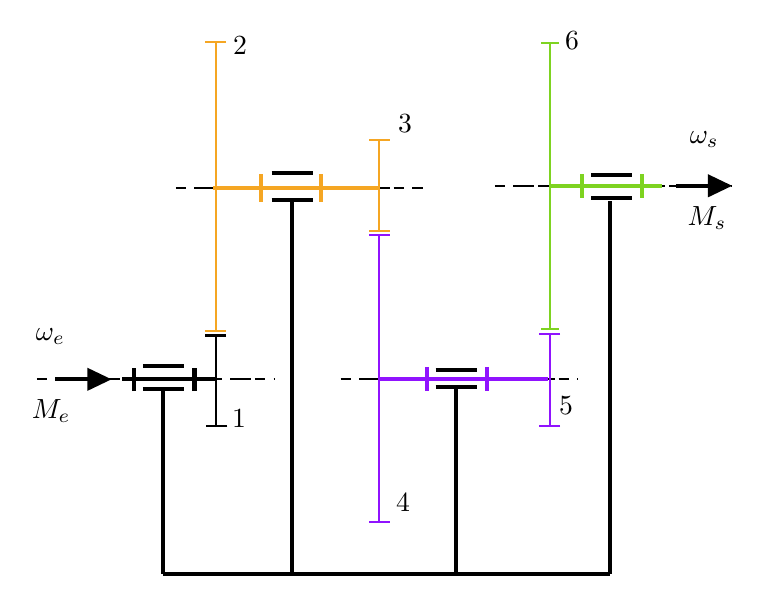
\begin{tikzpicture}[x=0.75pt,y=0.75pt,yscale=-1,xscale=1]
		%uncomment if require: \path (0,1161); %set diagram left start at 0, and has height of 1161
		
		%Straight Lines [id:da33961155809250365] 
		\draw  [dash pattern={on 3.75pt off 3pt on 7.5pt off 1.5pt}]  (263.32,205.15) -- (377.62,205.15) ;
		%Straight Lines [id:da8162384842911465] 
		\draw  [dash pattern={on 3.75pt off 3pt on 7.5pt off 1.5pt}]  (183.86,113.14) -- (302.86,113.14) ;
		%Straight Lines [id:da6060961967729845] 
		\draw [color={rgb, 255:red, 245; green, 166; blue, 35 }  ,draw opacity=1 ][line width=1.5]    (202,113.14) -- (281.86,113.14) ;
		%Straight Lines [id:da6471440269690474] 
		\draw [color={rgb, 255:red, 245; green, 166; blue, 35 }  ,draw opacity=1 ][line width=1.5]    (225,106.5) -- (225,119.78) ;
		%Straight Lines [id:da16702576745293607] 
		\draw [color={rgb, 255:red, 245; green, 166; blue, 35 }  ,draw opacity=1 ][line width=1.5]    (254,106.5) -- (254,119.78) ;
		%Straight Lines [id:da07315360896479906] 
		\draw [color={rgb, 255:red, 245; green, 166; blue, 35 }  ,draw opacity=1 ][line width=0.75]    (208.16,43) -- (197.92,43) ;
		%Straight Lines [id:da07391113584152431] 
		\draw [color={rgb, 255:red, 245; green, 166; blue, 35 }  ,draw opacity=1 ][line width=0.75]    (208,182) -- (197.86,182) ;
		%Straight Lines [id:da5340676599486716] 
		\draw [color={rgb, 255:red, 245; green, 166; blue, 35 }  ,draw opacity=1 ][line width=0.75]    (203.04,182.52) -- (203.04,43) ;
		%Straight Lines [id:da25918670266586474] 
		\draw [color={rgb, 255:red, 245; green, 166; blue, 35 }  ,draw opacity=1 ][line width=0.75]    (287,90) -- (276.86,90) ;
		%Straight Lines [id:da9387977229071487] 
		\draw [color={rgb, 255:red, 245; green, 166; blue, 35 }  ,draw opacity=1 ][line width=0.75]    (287,134) -- (276.86,134) ;
		%Straight Lines [id:da18226915476581196] 
		\draw [color={rgb, 255:red, 245; green, 166; blue, 35 }  ,draw opacity=1 ][line width=0.75]    (281.86,133.64) -- (281.86,90.36) ;
		%Straight Lines [id:da23655982826816135] 
		\draw [line width=1.5]    (230,106) -- (249.86,106) ;
		%Straight Lines [id:da3364667279398781] 
		\draw [line width=1.5]    (230,119) -- (249.86,119) ;
		%Straight Lines [id:da18700246864747294] 
		\draw [line width=1.5]    (168,199) -- (187.86,199) ;
		%Straight Lines [id:da8285221588880871] 
		\draw [line width=1.5]    (168,210) -- (187.86,210) ;
		%Straight Lines [id:da07473648772596375] 
		\draw [line width=1.5]    (177.86,210.01) -- (177.86,299.28) ;
		%Straight Lines [id:da3155752058098067] 
		\draw [line width=1.5]    (392.86,299.28) -- (177.86,299.28) ;
		%Straight Lines [id:da3877695918590758] 
		\draw [line width=1.5]    (392.86,299.28) -- (392.86,119.28) ;
		%Straight Lines [id:da1031299270196111] 
		\draw [line width=1.5]    (318.86,299.28) -- (318.86,209.01) ;
		%Straight Lines [id:da6999735516887908] 
		\draw [line width=1.5]    (239.86,299.28) -- (239.86,119.28) ;
		%Straight Lines [id:da5245713065529585] 
		\draw [line width=1.5]    (309,201) -- (328.86,201) ;
		%Straight Lines [id:da7965334886991164] 
		\draw [line width=1.5]    (309,209) -- (328.86,209) ;
		%Straight Lines [id:da7020019731795575] 
		\draw [line width=1.5]    (384,107) -- (403.86,107) ;
		%Straight Lines [id:da19255045358633538] 
		\draw [line width=1.5]    (384,118) -- (403.86,118) ;
		%Straight Lines [id:da6462495895463147] 
		\draw [line width=1.5]    (125.86,205.32) -- (148.86,205.32) ;
		\draw [shift={(152.86,205.32)}, rotate = 180] [fill={rgb, 255:red, 0; green, 0; blue, 0 }  ][line width=0.08]  [draw opacity=0] (11.61,-5.58) -- (0,0) -- (11.61,5.58) -- cycle    ;
		%Straight Lines [id:da6613455815055054] 
		\draw [line width=1.5]    (424.86,112.08) -- (447.86,112.08) ;
		\draw [shift={(451.86,112.08)}, rotate = 180] [fill={rgb, 255:red, 0; green, 0; blue, 0 }  ][line width=0.08]  [draw opacity=0] (11.61,-5.58) -- (0,0) -- (11.61,5.58) -- cycle    ;
		%Straight Lines [id:da09048724569773259] 
		\draw [color={rgb, 255:red, 0; green, 0; blue, 0 }  ,draw opacity=1 ][line width=0.75]    (203.04,228.32) -- (203.04,184.57) ;
		%Straight Lines [id:da6756170197111613] 
		\draw [color={rgb, 255:red, 0; green, 0; blue, 0 }  ,draw opacity=1 ][line width=0.75]    (208.16,184.2) -- (197.92,184.2) ;
		%Straight Lines [id:da932294290362093] 
		\draw [color={rgb, 255:red, 0; green, 0; blue, 0 }  ,draw opacity=1 ][line width=0.75]    (208.67,228) -- (198.53,228) ;
		%Straight Lines [id:da8247593165970979] 
		\draw [color={rgb, 255:red, 0; green, 0; blue, 0 }  ,draw opacity=1 ][line width=1.5]    (157.98,205.32) -- (203.2,205.32) ;
		%Straight Lines [id:da7452297395950489] 
		\draw [color={rgb, 255:red, 0; green, 0; blue, 0 }  ,draw opacity=1 ][line width=1.5]    (163.86,210.98) -- (163.86,199.67) ;
		%Straight Lines [id:da4099575056003457] 
		\draw [color={rgb, 255:red, 0; green, 0; blue, 0 }  ,draw opacity=1 ][line width=1.5]    (192.86,210.98) -- (192.86,199.67) ;
		%Straight Lines [id:da9684985519961828] 
		\draw  [dash pattern={on 3.75pt off 3pt on 7.5pt off 1.5pt}]  (116.98,205.32) -- (231.29,205.32) ;
		%Straight Lines [id:da33891220737858907] 
		\draw [color={rgb, 255:red, 144; green, 19; blue, 254 }  ,draw opacity=1 ][line width=0.75]    (287,136) -- (276.86,136) ;
		%Straight Lines [id:da7352390263466706] 
		\draw [color={rgb, 255:red, 144; green, 19; blue, 254 }  ,draw opacity=1 ][line width=0.75]    (287,274) -- (276.86,274) ;
		%Straight Lines [id:da35130408923394185] 
		\draw [color={rgb, 255:red, 144; green, 19; blue, 254 }  ,draw opacity=1 ][line width=0.75]    (281.98,136) -- (281.98,274.31) ;
		%Straight Lines [id:da5977895921900764] 
		\draw [color={rgb, 255:red, 144; green, 19; blue, 254 }  ,draw opacity=1 ][line width=0.75]    (369,183.33) -- (358.86,183.33) ;
		%Straight Lines [id:da8395035083373401] 
		\draw [color={rgb, 255:red, 144; green, 19; blue, 254 }  ,draw opacity=1 ][line width=0.75]    (369,228) -- (358.86,228) ;
		%Straight Lines [id:da8251863527489236] 
		\draw [color={rgb, 255:red, 144; green, 19; blue, 254 }  ,draw opacity=1 ][line width=0.75]    (363.93,183.15) -- (363.93,227.15) ;
		%Straight Lines [id:da7041594922573156] 
		\draw [color={rgb, 255:red, 144; green, 19; blue, 254 }  ,draw opacity=1 ][line width=1.5]    (281.33,205.15) -- (363.32,205.15) ;
		%Straight Lines [id:da24638750467494086] 
		\draw [color={rgb, 255:red, 144; green, 19; blue, 254 }  ,draw opacity=1 ][line width=1.5]    (304.98,199.32) -- (304.98,210.99) ;
		%Straight Lines [id:da9497257952934224] 
		\draw [color={rgb, 255:red, 144; green, 19; blue, 254 }  ,draw opacity=1 ][line width=1.5]    (333.65,199.32) -- (333.65,205.99) -- (333.65,210.99) ;
		%Straight Lines [id:da9240202784283811] 
		\draw [color={rgb, 255:red, 126; green, 211; blue, 33 }  ,draw opacity=1 ][line width=0.75]    (363.93,180.58) -- (363.93,46.25) -- (363.93,43.58) ;
		%Straight Lines [id:da6227457398066218] 
		\draw [color={rgb, 255:red, 126; green, 211; blue, 33 }  ,draw opacity=1 ][line width=0.75]    (368.27,43.25) -- (359.6,43.25) ;
		%Straight Lines [id:da2887531606034459] 
		\draw [color={rgb, 255:red, 126; green, 211; blue, 33 }  ,draw opacity=1 ][line width=0.75]    (368.27,181.25) -- (359.6,181.25) ;
		%Straight Lines [id:da455429012497387] 
		\draw  [dash pattern={on 3.75pt off 3pt on 7.5pt off 1.5pt}]  (337.56,112.08) -- (451.86,112.08) ;
		%Straight Lines [id:da16935007122750734] 
		\draw [color={rgb, 255:red, 126; green, 211; blue, 33 }  ,draw opacity=1 ][line width=1.5]    (363.86,112.08) -- (418.32,112.08) ;
		%Straight Lines [id:da44505019232990395] 
		\draw [color={rgb, 255:red, 126; green, 211; blue, 33 }  ,draw opacity=1 ][line width=1.5]    (379.65,106.41) -- (379.65,117.75) ;
		%Straight Lines [id:da9227978991118302] 
		\draw [color={rgb, 255:red, 126; green, 211; blue, 33 }  ,draw opacity=1 ][line width=1.5]    (408.65,106.41) -- (408.65,117.75) ;
		
		% Text Node
		\draw (115,179.4) node [anchor=north west][inner sep=0.75pt]    {$\omega _{e}$};
		% Text Node
		\draw (113,213.4) node [anchor=north west][inner sep=0.75pt]    {$M_{e}$};
		% Text Node
		\draw (429,120.4) node [anchor=north west][inner sep=0.75pt]    {$M_{s}$};
		% Text Node
		\draw (430,84.4) node [anchor=north west][inner sep=0.75pt]    {$\omega _{s}$};
		% Text Node
		\draw (209.5,218.4) node [anchor=north west][inner sep=0.75pt]    {$1$};
		% Text Node
		\draw (210,38.9) node [anchor=north west][inner sep=0.75pt]    {$2$};
		% Text Node
		\draw (289.5,76.4) node [anchor=north west][inner sep=0.75pt]    {$3$};
		% Text Node
		\draw (288.5,258.9) node [anchor=north west][inner sep=0.75pt]    {$4$};
		% Text Node
		\draw (367,212.4) node [anchor=north west][inner sep=0.75pt]    {$5$};
		% Text Node
		\draw (370,36.4) node [anchor=north west][inner sep=0.75pt]    {$6$};
		\end{tikzpicture}
		\vspace*{3mm}	
		\caption{Equivalent gear train example in 2D with multiple wheels}
	\end{figure}
	The overall transmission ratio will then be given for the speed of rotation by:
	
	where the fourth equality is simplified because in the case above:
	
	We can also express the total transmission in terms of diameters. Since we have proven that:
	
	it then comes immediately:
	
	expression that we can not simplify!
	\begin{tcolorbox}[title=Remark,arc=10pt,breakable,drop lifted shadow,
  skin=enhanced,
  skin first is subskin of={enhancedfirst}{arc=10pt,no shadow},
  skin middle is subskin of={enhancedmiddle}{arc=10pt,no shadow},
  skin last is subskin of={enhancedlast}{drop lifted shadow}]
	Thus, in the context of a transmission of a watch with astronomical complication, the transmission ratio was obtained by determining the rational fraction $1802/217$. This being very difficult to implement with only two gears, we'll just build with three axes and four gears (with $7$, $31$, $34$ and $53$ teeth) the same ratio - which fortunately is not irreducible - as follows:
	
	\end{tcolorbox}
	\begin{tcolorbox}[colframe=black,colback=white,sharp corners,breakable]
	\textbf{{\Large \ding{45}}Example:}\\\\
	We would like with a $4$ wheel gear train on $2$ axes, driven by the time axis (which spins through $12$ hours), make a very precise transmission ratio $r$, to make a watch complication that shows a Moon phase with the classic disc having $2$ Moons and turning behind a mask:
	\begin{figure}[H]
		\centering
		\begin{subfigure}{0.4\textwidth}
			\includegraphics[width=\textwidth]{img/engineering/moon_phase_disc.jpg}
		\end{subfigure}
		\begin{subfigure}{0.4\textwidth}
			\includegraphics[width=\textwidth]{img/engineering/moon_phase_mask.jpg}
		\end{subfigure}				
	\end{figure}
	As constraints the maximum number of teeth per wheel shall not exceed $300$ teeth and do not fall below $7$. The accuracy will be the best permitted within these numbers of teeth.\\
	
	We will take $29$ days $12$ hours and $44$ minutes for the lunar month.\\
		
	The calculation of the desired ratio is relatively simple. The two Moons disc must make a full turn in $5,102,885.8$ seconds. The wheel of the timepiece makes one revolution in $12$ hours, or $43,200$ seconds.\\
		
	For a turn of the two Moons disc (leading axis) the axis of the $12$h wheel (driven axis):
	
	and rounding as below, we have an error of about $3$ ten-thousandth of a second per $12$ hours. Approximately $0.2$ seconds per year of delay. What is acceptable for a mechanical watch.\\

	By rounding:
	
	we have an error of about $30$ seconds per year, which is still acceptable for a mechanical watch. If we take again away one decimal place, then we have a delay of $6$ minutes per year, even removing an additional decimal place, we would have a $49$ minutes delay (which is still acceptable for many mechanical watches). By cons, beyond, this is no longer acceptable!\\
	
	Now, to find the nearest decomposable rational fraction to this number there exist numerous empirical methods (by trial and error or by using a Brocot tree) and tables but the least worst ... for us ... is that using the continuous fractions (\SeeChapter{see section Number Theory page \pageref{continued fraction}}) when it is applicable...\\
	
	Remember that we have proved that:
	
	considering:
	
	If we denote by $x$ the ratio $a / b$ then the relations above give us that $q_1$ is the integer part of $x$, $q_2$ the integer part of $b/r_1$ thus of $b/((x-q_1)b)=1/(x-q_1)$ either and so on...\\
	
	We then have in our case:
	
	Thus after we put everything to a common denominator:
	
	If the difference (error) between this fraction and the exact value is acceptable (just have to calculate the error of time this causes after a year of operation of the watch for example), we stop ourselves here. But there is a second criterion ... the numerator and denominator must be decomposable in a satisfactory manner in relation to requirements of the number of teeth of the gears. Or in this case, the denominator ($5788$) can not be decomposed satisfactorily in relation to our constraints (do the decomposition with the command \texttt{ifactor} of Maple 4.00b and you will see!).\\
	
	If we continue to develop our continued fraction, we will not find an acceptable solution before the numerator or the denominator exceeds the maximum permissible value of $300^2$.\\

	Thus, we return for example to our fraction (well this is not an acceptable approximation because in reality the maladjustment of the watch will be too fast):
	
	and we cheat a bit by trial and error to find a good ratio:
	
	Then, as we have a four gears train, we must have:
	
	and then we take (always helping with the function \texttt{ifactor} of Maple 4.00b):
	
	\end{tcolorbox}
	
	\paragraph{Odd/Even Gear "problem"}\mbox{}\\\\
	The gear association below has a \underline{closed loop} of four different gears. No two of them have the same diameter, and no two have the same number of teeth. They turn smoothly. Any even number of gears, with parallel axles, or even smooth wheels, can be put into such a loop, and they will turn freely, no matter what their tooth count or size. There's a simple way to prove this, using elementary geometry.
	\begin{figure}[H]
		\begin{center}
			\includegraphics{img/engineering/even_loop_gear.jpg}
		\end{center}	
	\end{figure}
	The underlying principle isn't physics, but geometry, and it applies not only to gears, but to smooth friction wheels as well. The figure shows two friction wheels of different diameter. When they turn without slipping, the two circles must turn through the same arc, but in opposite sense of rotation. That is, if the left wheel turns clockwise through arc $A$, the right wheel turns counter-clockwise through arc $B$, and $B = - A$:
	\begin{figure}[H]
		\centering
		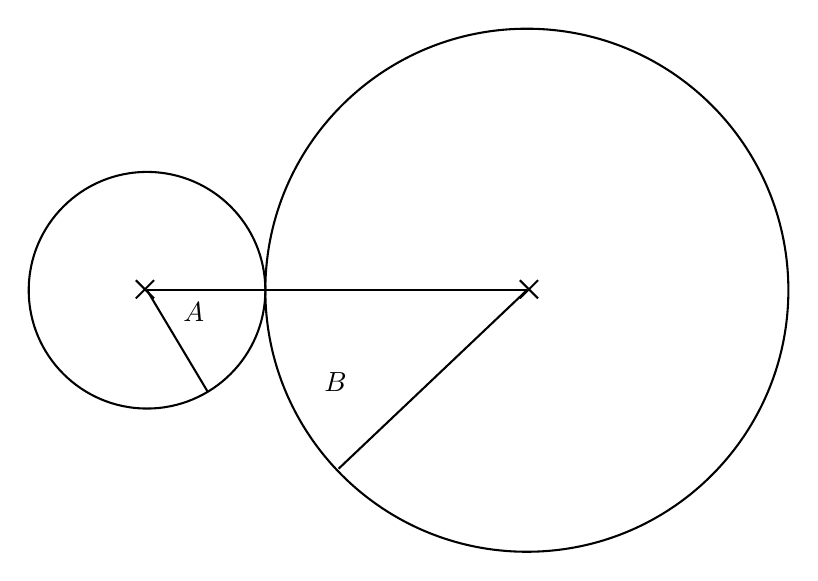
\begin{tikzpicture}[x=0.75pt,y=0.75pt,yscale=-1,xscale=1]
		%uncomment if require: \path (0,428); %set diagram left start at 0, and has height of 428
		
		%Shape: Circle [id:dp8316596573653681] 
		\draw   (171,142) .. controls (171,110.52) and (196.52,85) .. (228,85) .. controls (259.48,85) and (285,110.52) .. (285,142) .. controls (285,173.48) and (259.48,199) .. (228,199) .. controls (196.52,199) and (171,173.48) .. (171,142) -- cycle ;
		%Shape: Circle [id:dp9147783350653504] 
		\draw   (285,142) .. controls (285,72.41) and (341.41,16) .. (411,16) .. controls (480.59,16) and (537,72.41) .. (537,142) .. controls (537,211.59) and (480.59,268) .. (411,268) .. controls (341.41,268) and (285,211.59) .. (285,142) -- cycle ;
		%Straight Lines [id:da7879604749812579] 
		\draw    (228,142) -- (411,142) ;
		\draw   (222.62,137.17) -- (231.38,145.92)(231.38,137.17) -- (222.62,145.92) ;
		\draw   (407.62,137.17) -- (416.38,145.92)(416.38,137.17) -- (407.62,145.92) ;
		%Straight Lines [id:da2543223953888194] 
		\draw    (228,142) -- (257.3,191) ;
		%Straight Lines [id:da15051080414927687] 
		\draw    (411,142) -- (320.3,228) ;
		
		% Text Node
		\draw (244,146.4) node [anchor=north west][inner sep=0.75pt]    {$A$};
		% Text Node
		\draw (312,180.4) node [anchor=north west][inner sep=0.75pt]    {$B$};
		
		\end{tikzpicture}	
	\end{figure}
	If these were gears, then if one gear turns through $N$ teeth, the other gear turns through $N$ teeth in the other direction. It follows that if you had a string of an odd number of gears and tried to make a loop by meshing the gears at the end of the loop, their points of contact would be moving in opposite directions. If you closed a loop of an even number of gears, they would all turn quite smoothly through the same arc.
	
	There are even exotic gears that have non-circular perimeters, such as oval or elliptical. You could make a model with an even number of these in a loop, and the gears in the model would turn smoothly.
	
	A typical mistake is to think that the following will work:
	\begin{figure}[H]
		\centering
		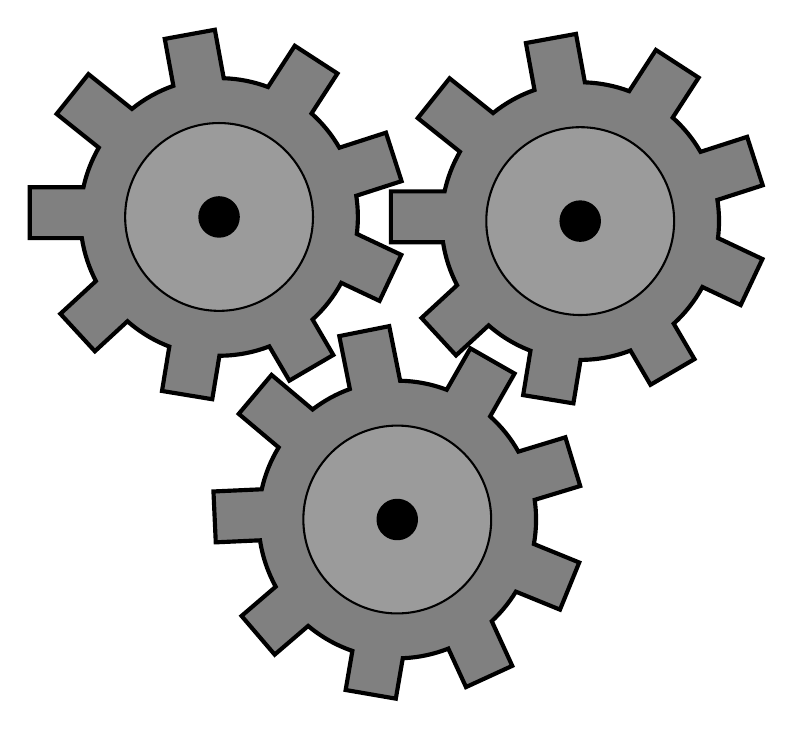
\begin{tikzpicture}[x=0.75pt,y=0.75pt,yscale=-1,xscale=1]
		%uncomment if require: \path (0,1046); %set diagram left start at 0, and has height of 1046
		
		%Shape: Path Data [id:dp45447415104798816] 
		\draw  [fill={rgb, 255:red, 128; green, 128; blue, 128 }  ,fill opacity=1 ][line width=1.5]  (304.13,210.25) .. controls (304.13,213.01) and (303.96,215.74) .. (303.63,218.42) -- (325.04,228.52) -- (314.57,250.71) -- (296.12,242) .. controls (292.53,248.65) and (287.85,254.61) .. (282.31,259.66) -- (292.29,276.74) -- (271.11,289.11) -- (261.46,272.61) .. controls (254,275.51) and (245.89,277.1) .. (237.42,277.12) -- (233.97,298.07) -- (209.76,294.09) -- (213.28,272.7) .. controls (205.82,269.84) and (199.01,265.68) .. (193.12,260.5) -- (177.42,274.96) -- (160.79,256.92) -- (177.92,241.14) .. controls (174.6,234.78) and (172.28,227.82) .. (171.15,220.47) -- (146.04,220.47) -- (146.04,195.94) -- (171.91,195.94) .. controls (173.39,189.13) and (175.92,182.71) .. (179.3,176.85) -- (158.99,160.62) -- (174.31,141.45) -- (195.26,158.2) .. controls (201.17,153.42) and (207.91,149.64) .. (215.23,147.09) -- (211.09,124.47) -- (235.22,120.06) -- (239.5,143.41) .. controls (246.98,143.66) and (254.16,145.14) .. (260.83,147.65) -- (273.72,127.79) -- (294.3,141.14) -- (281.81,160.38) .. controls (287.11,165.12) and (291.65,170.69) .. (295.22,176.89) -- (317.66,169.65) -- (325.19,193) -- (303.35,200.05) .. controls (303.86,203.37) and (304.13,206.78) .. (304.13,210.25) -- cycle ;
		%Shape: Circle [id:dp20020998396584977] 
		\draw  [fill={rgb, 255:red, 155; green, 155; blue, 155 }  ,fill opacity=1 ] (192,210.25) .. controls (192,185.26) and (212.26,165) .. (237.25,165) .. controls (262.24,165) and (282.5,185.26) .. (282.5,210.25) .. controls (282.5,235.24) and (262.24,255.5) .. (237.25,255.5) .. controls (212.26,255.5) and (192,235.24) .. (192,210.25) -- cycle ;
		%Shape: Circle [id:dp1910572610533996] 
		\draw  [fill={rgb, 255:red, 0; green, 0; blue, 0 }  ,fill opacity=1 ] (227.75,210.25) .. controls (227.75,205) and (232,200.75) .. (237.25,200.75) .. controls (242.5,200.75) and (246.75,205) .. (246.75,210.25) .. controls (246.75,215.5) and (242.5,219.75) .. (237.25,219.75) .. controls (232,219.75) and (227.75,215.5) .. (227.75,210.25) -- cycle ;
		
		%Shape: Path Data [id:dp24196046889878198] 
		\draw  [fill={rgb, 255:red, 128; green, 128; blue, 128 }  ,fill opacity=1 ][line width=1.5]  (478.13,212.25) .. controls (478.13,215.01) and (477.96,217.74) .. (477.63,220.42) -- (499.04,230.52) -- (488.57,252.71) -- (470.12,244) .. controls (466.53,250.65) and (461.85,256.61) .. (456.31,261.66) -- (466.29,278.74) -- (445.11,291.11) -- (435.46,274.61) .. controls (428,277.51) and (419.89,279.1) .. (411.42,279.12) -- (407.97,300.07) -- (383.76,296.09) -- (387.28,274.7) .. controls (379.82,271.84) and (373.01,267.68) .. (367.12,262.5) -- (351.42,276.96) -- (334.79,258.92) -- (351.92,243.14) .. controls (348.6,236.78) and (346.28,229.82) .. (345.15,222.47) -- (320.04,222.47) -- (320.04,197.94) -- (345.91,197.94) .. controls (347.39,191.13) and (349.92,184.71) .. (353.3,178.85) -- (332.99,162.62) -- (348.31,143.45) -- (369.26,160.2) .. controls (375.17,155.42) and (381.91,151.64) .. (389.23,149.09) -- (385.09,126.47) -- (409.22,122.06) -- (413.5,145.41) .. controls (420.98,145.66) and (428.16,147.14) .. (434.83,149.65) -- (447.72,129.79) -- (468.3,143.14) -- (455.81,162.38) .. controls (461.11,167.12) and (465.65,172.69) .. (469.22,178.89) -- (491.66,171.65) -- (499.19,195) -- (477.35,202.05) .. controls (477.86,205.37) and (478.13,208.78) .. (478.13,212.25) -- cycle ;
		%Shape: Circle [id:dp21663098621403432] 
		\draw  [fill={rgb, 255:red, 155; green, 155; blue, 155 }  ,fill opacity=1 ] (366,212.25) .. controls (366,187.26) and (386.26,167) .. (411.25,167) .. controls (436.24,167) and (456.5,187.26) .. (456.5,212.25) .. controls (456.5,237.24) and (436.24,257.5) .. (411.25,257.5) .. controls (386.26,257.5) and (366,237.24) .. (366,212.25) -- cycle ;
		%Shape: Circle [id:dp4973011565363836] 
		\draw  [fill={rgb, 255:red, 0; green, 0; blue, 0 }  ,fill opacity=1 ] (401.75,212.25) .. controls (401.75,207) and (406,202.75) .. (411.25,202.75) .. controls (416.5,202.75) and (420.75,207) .. (420.75,212.25) .. controls (420.75,217.5) and (416.5,221.75) .. (411.25,221.75) .. controls (406,221.75) and (401.75,217.5) .. (401.75,212.25) -- cycle ;
		
		%Shape: Path Data [id:dp8344368676828224] 
		\draw  [fill={rgb, 255:red, 128; green, 128; blue, 128 }  ,fill opacity=1 ][line width=1.5]  (374.27,399.08) .. controls (372.49,401.2) and (370.61,403.18) .. (368.64,405.01) -- (378.51,426.53) -- (356.22,436.76) -- (347.71,418.22) .. controls (340.68,421) and (333.25,422.55) .. (325.77,422.85) -- (322.41,442.33) -- (298.23,438.16) -- (301.48,419.33) .. controls (293.91,416.74) and (286.67,412.74) .. (280.17,407.3) -- (264.05,421.11) -- (248.09,402.48) -- (264.55,388.38) .. controls (260.69,381.38) and (258.16,373.81) .. (256.98,366.05) -- (235.66,367.02) -- (234.55,342.51) -- (257.82,341.46) .. controls (259.38,334.46) and (262.08,327.64) .. (265.95,321.29) -- (246.73,305.12) -- (262.53,286.35) -- (282.32,303.01) .. controls (287.84,298.75) and (293.91,295.46) .. (300.27,293.16) -- (295.18,267.66) -- (319.24,262.86) -- (324.49,289.16) .. controls (332.08,289.31) and (339.68,290.76) .. (346.92,293.52) -- (358.32,273.55) -- (379.62,285.71) -- (367.86,306.33) .. controls (373.43,311.34) and (377.97,317.09) .. (381.45,323.31) -- (404.1,316.41) -- (411.25,339.88) -- (389.31,346.56) .. controls (390.31,353.6) and (390.2,360.78) .. (388.94,367.83) -- (410.77,376.73) -- (401.5,399.45) -- (380.25,390.78) .. controls (378.5,393.65) and (376.51,396.43) .. (374.27,399.08) -- cycle ;
		%Shape: Circle [id:dp03955969141576432] 
		\draw  [fill={rgb, 255:red, 155; green, 155; blue, 155 }  ,fill opacity=1 ] (288.48,326.89) .. controls (304.57,307.77) and (333.12,305.31) .. (352.24,321.4) .. controls (371.36,337.49) and (373.82,366.04) .. (357.73,385.16) .. controls (341.64,404.28) and (313.09,406.74) .. (293.97,390.65) .. controls (274.85,374.56) and (272.39,346.01) .. (288.48,326.89) -- cycle ;
		%Shape: Circle [id:dp6564170679624783] 
		\draw  [fill={rgb, 255:red, 0; green, 0; blue, 0 }  ,fill opacity=1 ] (315.83,349.91) .. controls (319.21,345.89) and (325.21,345.38) .. (329.22,348.76) .. controls (333.23,352.13) and (333.75,358.13) .. (330.37,362.14) .. controls (326.99,366.16) and (321,366.67) .. (316.99,363.29) .. controls (312.97,359.91) and (312.46,353.92) .. (315.83,349.91) -- cycle ;
		
		\end{tikzpicture}
	\end{figure}
	
	\subsubsection{Types of Gears}
	Here are some basic types of gears and how they are different from each other.
	
	\begin{itemize}
		\item The most common gears are "\NewTerm{spur gears}\index{spur gear}" and are used as we have seen previously in series for large gear reductions along a same plane! The teeth on spur gears are straight and are mounted in parallel on different shafts. These are particularly loud, due to the gear tooth engaging and colliding. Each impact makes loud noises and causes vibration, which is why spur gears are not used in machinery like cars. 

		\item "\NewTerm{Helical gears}\index{helical gears}" operate more smoothly and quietly compared to spur gears due to the way the teeth interact. The teeth on a helical gear cut at an angle to the face of the gear. When two of the teeth start to engage, the contact is gradual--starting at one end of the tooth and maintaining contact as the gear rotates into full engagement. Helical is the most commonly used gear in transmissions.

		\item "\NewTerm{Bevel gears}\index{bevel gear}" are used to change the direction of a shaft's rotation (bevel gears are most often mounted on shafts that are 90 degrees apart). Bevel gears have teeth that are available in straight, spiral, or hypoid shape. Straight teeth have similar characteristics to spur gears and also have a large impact when engaged.

		\item "\NewTerm{Worm gears}\index{worm gears}" are used in large gear reductions. The setup is designed so that the worm can turn the gear, but the gear cannot turn the worm. The angle of the worm is shallow and as a result the gear is held in place due to the friction between the two. The gear is found in applications such as conveyor systems in which the locking feature can act as a brake or an emergency stop.
		
		\item "\NewTerm{Geneva gears}\index{Geneva gears}" or "\NewTerm{Maltese cross gears}\index{Maltese cross gears}" are gears mechanism that translates a continuous rotation into an intermittent rotary motion. The rotating drive wheel has a pin that reaches into a slot of the driven wheel advancing it by one step. The drive wheel also has a raised circular blocking disc that locks the driven wheel in position between steps. In the most common arrangement, the driven wheel has four slots and thus advances by one step of $90^\circ$ for each rotation of the drive wheel. If the driven wheel has n slots, it advances by $360^\circ/n$ per full rotation of the drive wheel.
		
		\item ...
	\end{itemize}
	In the figure below the reader can see a photo and the name of the nine most common types of gears used in engineering:
	\begin{figure}[H]
		\centering
		\includegraphics[scale=0.9]{img/engineering/types_of_gear.jpg}
		\caption{Most common types of gears}
	\end{figure}
	While manual transmissions (manually shifting a gear selector mechanism that disengages one gear and selects another) have remained relatively unchanged over the years, electronically controlled automatic, semi-automatic, and continuously variable transmissions (CVTs) have become increasingly complex, but also easier to use than ever before. However, modern transmissions of all types have become more prone to failure, primarily because of this higher level of complexity.
	
	The Continuously Variable Transmissions (CVT) is a transmission mechanism that doesn't use gears as its means of producing various vehicle speeds at different engine speeds. Instead of gears, the system relies on a rubber or metal belt running over pulleys that can vary their effective diameters:
	\begin{figure}[H]
		\centering
		\includegraphics{img/engineering/cvt.jpg}
		\caption{Continuously Variable Transmissions (CVT)}
	\end{figure}
	To keep the belt at its optimum tension, one pulley will increase its effective diameter, while the other decreases its effective diameter by exactly the same amount. This action is exactly analogous to the effect produced when gears of different diameters are engaged.
	
	Now just a word about epicyclic gears\label{epicyclic gears}!
	
	\textbf{Definition (\#\thesection.\mydef):} An "\NewTerm{epicyclic gear train}\index{epicyclic gear train}" or "\NewTerm{planetary gear}\index{planetary gear}" consists of two gears mounted so that the center of one gear revolves around the center of the other. A carrier connects the centers of the two gears and rotates to carry one gear, named the "planet gear", around the other, named the "sun gear". The planet and sun gears mesh so that their pitch circles roll without slip. A point on the pitch circle of the planet gear traces an epicycloid curve. In this simplified case, the sun gear is fixed and the planetary gear(s) roll around the sun gear.
	
	The epicyclic gear train below consists of a sun gear (yellow), planet gears (blue) supported by the carrier (green) and an annular gear (pink). The red marks show the relative displacement of the sun gear and carrier, when the carrier is rotated $45^\circ$ clockwise and the annular gear is held fixed:
	\begin{figure}[H]
		\centering
		\includegraphics[scale=0.5]{img/engineering/epicyclic_gear_train.jpg}
		\caption[Epicyclic gear]{Epicyclic gear (source: Wikipedia)}
	\end{figure}
	Yes ok... but why use a epicyclic train gear excepted in watches knowing that the latter or not one of the most important thing in life!
	
	There is one well known example: modern cars using CVT (and not only) have epicyclic gears and also almost all bicycles:
	\begin{figure}[H]
		\centering
		\includegraphics{img/mechanics/bycicle_gear.jpg}
		\caption{Bicycle hub gear (special example)}
	\end{figure}

	Why do CVT and bicycles use this type of gear? 
	
	First because this type of gear is very compact in surface and in volume and as forces are distributed across $4$ planets gears (sometimes more!) the effort on the sun gear is divided. This is for the technical point of view...
	
	Now for the utility point of view: Consider the figure above, where for example the sun gear is driven by the motor of the car and the annular gear  is connected in one way or another to the transmission of the car. Therefore if we make the sun gear and the carrier solidary (connected) they turn together in the same direction. Then we speak of "\NewTerm{forward gear}\index{forward gear}" as the whole mechanism move as a single unique gear. If we remove what makes the sun gear and annular solidary than as it is a double epicyclic gear, the sun gear will force the annular gear to turn in the reverse direction and then we get a "\NewTerm{reverse gear}\index{reverse gear}".
	\begin{tcolorbox}[title=Remark,arc=10pt,breakable,drop lifted shadow,
  skin=enhanced,
  skin first is subskin of={enhancedfirst}{arc=10pt,no shadow},
  skin middle is subskin of={enhancedmiddle}{arc=10pt,no shadow},
  skin last is subskin of={enhancedlast}{drop lifted shadow}]
	If the reader wants to see such a gear in action he can take a look to YouTube where there is a ton of video on this subject.
	\end{tcolorbox}
	The gear ratio of an epicyclic gearing system is somewhat non-intuitive, particularly because there are several ways in which an input rotation can be converted into an output rotation. Indeed, in some hybrid vehicle transmissions, two of the components are used as inputs with the third providing output relative to the two inputs!!
	
	OK let us now introduce some mathematical properties of this gear. For this let us consider the following figure where for simplification purposes our epicyclic has its planetary gears that are horizontal:
	\begin{figure}[H]
		\centering
		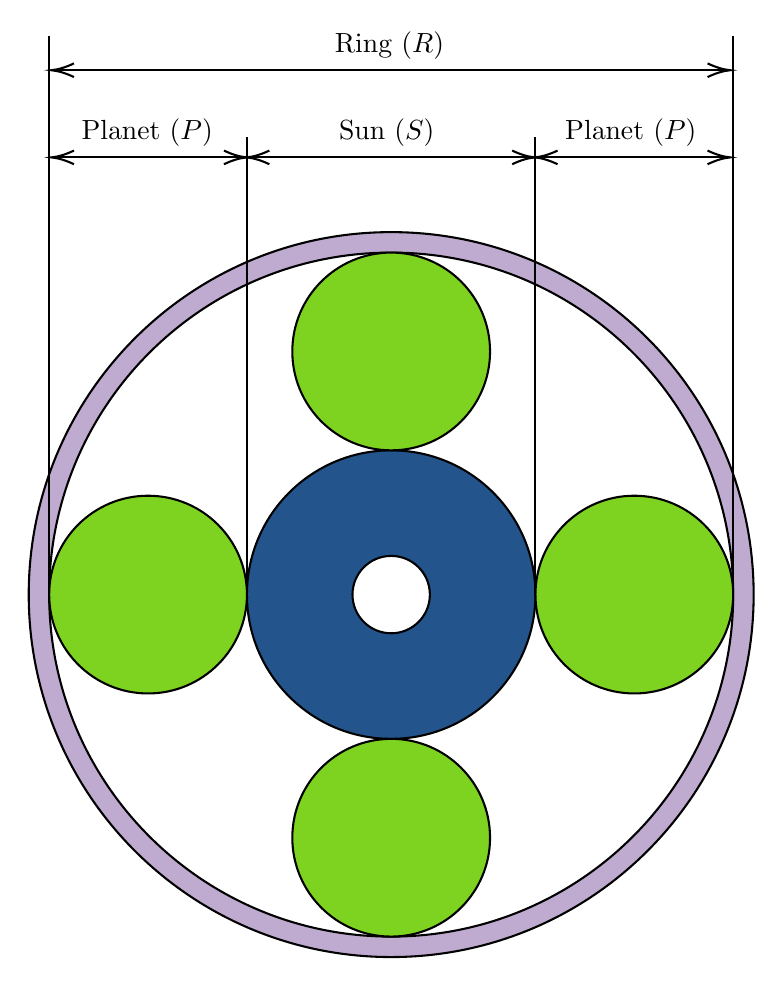
\begin{tikzpicture}[x=0.75pt,y=0.75pt,yscale=-1,xscale=1]
		%uncomment if require: \path (0,1500); %set diagram left start at 0, and has height of 1500
		
		%Shape: Donut [id:dp5481749165752765] 
		\draw  [fill={rgb, 255:red, 192; green, 171; blue, 208 }  ,fill opacity=1 ,even odd rule] (153.86,295.64) .. controls (153.86,204.63) and (227.63,130.86) .. (318.64,130.86) .. controls (409.64,130.86) and (483.41,204.63) .. (483.41,295.64) .. controls (483.41,386.64) and (409.64,460.41) .. (318.64,460.41) .. controls (227.63,460.41) and (153.86,386.64) .. (153.86,295.64)(144,295.64) .. controls (144,199.19) and (222.19,121) .. (318.64,121) .. controls (415.09,121) and (493.27,199.19) .. (493.27,295.64) .. controls (493.27,392.09) and (415.09,470.27) .. (318.64,470.27) .. controls (222.19,470.27) and (144,392.09) .. (144,295.64) ;
		%Shape: Donut [id:dp012855901397784919] 
		\draw  [fill={rgb, 255:red, 35; green, 84; blue, 140 }  ,fill opacity=1 ,even odd rule] (300,295.64) .. controls (300,285.34) and (308.34,277) .. (318.64,277) .. controls (328.93,277) and (337.27,285.34) .. (337.27,295.64) .. controls (337.27,305.93) and (328.93,314.27) .. (318.64,314.27) .. controls (308.34,314.27) and (300,305.93) .. (300,295.64)(249.14,295.64) .. controls (249.14,257.25) and (280.25,226.14) .. (318.64,226.14) .. controls (357.02,226.14) and (388.14,257.25) .. (388.14,295.64) .. controls (388.14,334.02) and (357.02,365.14) .. (318.64,365.14) .. controls (280.25,365.14) and (249.14,334.02) .. (249.14,295.64) ;
		%Shape: Circle [id:dp2314811419430689] 
		\draw  [fill={rgb, 255:red, 126; green, 211; blue, 33 }  ,fill opacity=1 ] (271,178.5) .. controls (271,152.19) and (292.33,130.86) .. (318.64,130.86) .. controls (344.95,130.86) and (366.27,152.19) .. (366.27,178.5) .. controls (366.27,204.81) and (344.95,226.14) .. (318.64,226.14) .. controls (292.33,226.14) and (271,204.81) .. (271,178.5) -- cycle ;
		%Shape: Circle [id:dp38896672275219335] 
		\draw  [fill={rgb, 255:red, 126; green, 211; blue, 33 }  ,fill opacity=1 ] (388.14,295.64) .. controls (388.14,269.33) and (409.46,248) .. (435.77,248) .. controls (462.08,248) and (483.41,269.33) .. (483.41,295.64) .. controls (483.41,321.95) and (462.08,343.27) .. (435.77,343.27) .. controls (409.46,343.27) and (388.14,321.95) .. (388.14,295.64) -- cycle ;
		%Shape: Circle [id:dp7705711516931659] 
		\draw  [fill={rgb, 255:red, 126; green, 211; blue, 33 }  ,fill opacity=1 ] (271,412.77) .. controls (271,386.46) and (292.33,365.14) .. (318.64,365.14) .. controls (344.95,365.14) and (366.27,386.46) .. (366.27,412.77) .. controls (366.27,439.08) and (344.95,460.41) .. (318.64,460.41) .. controls (292.33,460.41) and (271,439.08) .. (271,412.77) -- cycle ;
		%Shape: Circle [id:dp3396097172012975] 
		\draw  [fill={rgb, 255:red, 126; green, 211; blue, 33 }  ,fill opacity=1 ] (153.86,295.64) .. controls (153.86,269.33) and (175.19,248) .. (201.5,248) .. controls (227.81,248) and (249.14,269.33) .. (249.14,295.64) .. controls (249.14,321.95) and (227.81,343.27) .. (201.5,343.27) .. controls (175.19,343.27) and (153.86,321.95) .. (153.86,295.64) -- cycle ;
		%Straight Lines [id:da7128029779698084] 
		\draw    (153.86,26.27) -- (153.86,295.64) ;
		%Straight Lines [id:da8127694149766282] 
		\draw    (249.14,75.18) -- (249.14,295.64) ;
		%Straight Lines [id:da8432681741073249] 
		\draw    (388.14,75.18) -- (388.14,295.64) ;
		%Straight Lines [id:da39650972363941683] 
		\draw    (483.41,26.27) -- (483.41,295.64) ;
		%Straight Lines [id:da6119813400419791] 
		\draw    (247,85) -- (156.86,85) ;
		\draw [shift={(154.86,85)}, rotate = 360] [color={rgb, 255:red, 0; green, 0; blue, 0 }  ][line width=0.75]    (10.93,-3.29) .. controls (6.95,-1.4) and (3.31,-0.3) .. (0,0) .. controls (3.31,0.3) and (6.95,1.4) .. (10.93,3.29)   ;
		\draw [shift={(249,85)}, rotate = 180] [color={rgb, 255:red, 0; green, 0; blue, 0 }  ][line width=0.75]    (10.93,-3.29) .. controls (6.95,-1.4) and (3.31,-0.3) .. (0,0) .. controls (3.31,0.3) and (6.95,1.4) .. (10.93,3.29)   ;
		%Straight Lines [id:da7794324438169438] 
		\draw    (385.86,85) -- (251,85) ;
		\draw [shift={(249,85)}, rotate = 360] [color={rgb, 255:red, 0; green, 0; blue, 0 }  ][line width=0.75]    (10.93,-3.29) .. controls (6.95,-1.4) and (3.31,-0.3) .. (0,0) .. controls (3.31,0.3) and (6.95,1.4) .. (10.93,3.29)   ;
		\draw [shift={(387.86,85)}, rotate = 180] [color={rgb, 255:red, 0; green, 0; blue, 0 }  ][line width=0.75]    (10.93,-3.29) .. controls (6.95,-1.4) and (3.31,-0.3) .. (0,0) .. controls (3.31,0.3) and (6.95,1.4) .. (10.93,3.29)   ;
		%Straight Lines [id:da7667203047288647] 
		\draw    (480,85) -- (389.86,85) ;
		\draw [shift={(387.86,85)}, rotate = 360] [color={rgb, 255:red, 0; green, 0; blue, 0 }  ][line width=0.75]    (10.93,-3.29) .. controls (6.95,-1.4) and (3.31,-0.3) .. (0,0) .. controls (3.31,0.3) and (6.95,1.4) .. (10.93,3.29)   ;
		\draw [shift={(482,85)}, rotate = 180] [color={rgb, 255:red, 0; green, 0; blue, 0 }  ][line width=0.75]    (10.93,-3.29) .. controls (6.95,-1.4) and (3.31,-0.3) .. (0,0) .. controls (3.31,0.3) and (6.95,1.4) .. (10.93,3.29)   ;
		%Straight Lines [id:da8935167939599455] 
		\draw    (480,43) -- (156.86,43) ;
		\draw [shift={(154.86,43)}, rotate = 360] [color={rgb, 255:red, 0; green, 0; blue, 0 }  ][line width=0.75]    (10.93,-3.29) .. controls (6.95,-1.4) and (3.31,-0.3) .. (0,0) .. controls (3.31,0.3) and (6.95,1.4) .. (10.93,3.29)   ;
		\draw [shift={(482,43)}, rotate = 180] [color={rgb, 255:red, 0; green, 0; blue, 0 }  ][line width=0.75]    (10.93,-3.29) .. controls (6.95,-1.4) and (3.31,-0.3) .. (0,0) .. controls (3.31,0.3) and (6.95,1.4) .. (10.93,3.29)   ;
		
		% Text Node
		\draw (290,23) node [anchor=north west][inner sep=0.75pt]   [align=left] {Ring ($\displaystyle R$)};
		% Text Node
		\draw (168,65) node [anchor=north west][inner sep=0.75pt]   [align=left] {Planet ($\displaystyle P$)};
		% Text Node
		\draw (401,65) node [anchor=north west][inner sep=0.75pt]   [align=left] {Planet ($\displaystyle P$)};
		% Text Node
		\draw (292,65) node [anchor=north west][inner sep=0.75pt]   [align=left] {Sun ($\displaystyle S$)};
		\end{tikzpicture}
		\vspace*{3mm}
		\caption{Epicyclic gear simplified schema}
	\end{figure}
	From the figure above we want to prove a canonical relation for the tooth counts. For this purpose let us denote the number of teeth of the ring gear by $N_r$, of the sun gear by $N_s$, and of the planet gears by $N_p$.
	
	We will assume that our planetary gear to work out is that all teeth have the same pitch, or tooth spacing (this ensures that the teeth mesh).
	
	The determination of a canonical between all teeth can  be made more clear by imagining "gears" that just roll (no teeth), and imagine an even number of planet gears. From the illustration above we can see that the diameters of the sun gear, plus two planet gears be must equal to the ring gear size. That is:
	
	And if we assume that all teeth have the same pitch that we will denote here by $P$, that is:
	
	Therefore injecting and simplifying in the prior-previous relation we get:
	
	That is to say, the number of teeth in the ring gear is equal to the number of teeth in the middle sun gear plus twice the number of teeth in the planet gears.
	
	We see also that the special case $N_p=0$ brings us to the obvious result: $N_r=N_s$.
	
	Let us denote first by $\omega_r,\omega_s,\omega_p,\omega_c$  the angular velocity of respectively the Ring (annulus) gear (pink color in the first figure), Sun gear (yellow color in the first figure), Planet gears (blue color in the first figure) and Carrier (green color in the first figure) and $N_r,N_s,N_p$ the corresponding number of teeth of each gear (the Carrier no have teeth of sure!).
	
	To continue let us consider the following figure:
	\begin{figure}[H]
		\centering
		\includegraphics{img/engineering/linear_gear.jpg}
	\end{figure}
	A wheel (or gear) rolling without slipping as above means, any point on the circumference of the wheel will have both rotatory motion and translatory motion. Due to translation, if the velocity of the vehicle is $v$, then all the points of the wheel will have $v$ linear velocity in the forward direction. Then due to the rotatory motion, each point will have a linear velocity of $v = r\omega$, where $\omega$ is the angular velocity. For the top most point at a particular instant, the linear velocity will be horizontal forward. So at any instant, a top most point on the wheel will have two linear velocities of same magnitude:
	
	
	Now we have obviously (remember that $r$ denotes here the transmission ratio!):
	
	But we have immediately:
	
	We obviously have:
	
	But as just seen earlier above, we have:
	
	Therefore:
	
	Hence an important relation for the planetary gear:
	
	From that latter we get:
	
	This latter relation is in fact a special case of a more general one named the "\NewTerm{Willis equation}\index{Willis equation}" or "\NewTerm{fundamental formula of planetary gears}\index{fundamental formula of planetary gears}" for the case where the ring gear is fixed (blocked).

	Let us prove this equation:
	\begin{dem}
		If the sun gear stands still and the planet gear is locked firm on the carrier, then the swept angle of the carrier $\theta_c$ corresponds to the angular position of one of the planetary gear. Let us denoted this angular position $\theta_{p1}$.
	
		In fact, the planet gear will roll on the sun gear when mounted rotatable on the carrier and thus rotate around its own center of gravity. The planet gear will thus rotate by an additional angle $\theta_{p2}$.
	
		However we must not forget we have proved at the beginning of our study of simple gears systems:
		
		Therefore considering sill the sun gear as fix and the carrier gear as moving, we have:
		
		Therefore:
		
		Let us now consider that the carrier is held in position and the sun gear is rotated clockwise by an angle $\theta_s$. In this case, the planet gear will turn counter-clockwise by an angle $\theta_{p3}$. Analogous to the case before, the following statement applies (obviously the negative sign indicates that the motion of the planet gear is in the opposite direction to the motion of the sun gear): 
		
		Therefore:
		
		The motions of the planet gear according which have been considered separately so far, can now be superposed to the total motion:
		
		All this can be rearranged to the final relation we were looking for:
		
		That can also be rewritten as:
		
		\begin{flushright}
			$\blacksquare$  Q.E.D.
		\end{flushright}
	\end{dem}
	There are many other relations that we can derive for the planetary gear (we could write a whole book on the subject). But we will stop our investigations here because we are not big fans of the subject...
	
	\pagebreak
	\subsection{Strength of materials}
	Strength of materials (or SoM for the intimates...) is, like all the other sections of this book, an extremely vast area which level of detail and complexity of the calculations can explode rather quickly. We will in the following paragraphs focus on the essentials that the engineer (in business) needs to know. The developments are oversimplified for trivial special cases (straight bars and beams). In reality, we use the tensor calculus, design of experiments or computer modelling experience with FEM (finite element methods).
	
	Before we begin to study some simple concrete cases let us de some reminders of the proofs we have proceed during our study of this subject in the section of Continuum Mechanics:
	\begin{itemize}
		\item A solid considered as rigid does not exist, it is only a convenient approximation. Experience shows that a solid is in fact still slightly deformable under the effect of external forces.

		\item Relationships between deformations and tensions are usually complicated due to the anisotropy of the crystal lattices. However, the solids are generally not single crystals but polycrystalline substances consisting of assemblies of microcrystals associated randomly, they can be thus considered as isotropic.
	\end{itemize}
	Then, we should consider globally the following assumptions relatively to the developments that will follow:
	\begin{itemize}
		\item[H1.] Matter is homogeneous, that is to say for recall that it has the same physical constitution and the same structure throughout all its volume.

		\item[H2.] Matter is isotropic, that is to say for recall that its mechanical properties are the same in any point of the volume.

		\item[H3.] The material is perfectly elastic, that is to say, for recall that after removal of the external forces, the volume immediately takes back its original dimensions (unlike the plastic limit!).

		\item[H4.] The deformations (displacements of the points of the characteristics line ) are small compared with the dimensions of the objects studied.

		\item[H5.] Any straight section (cross-sections) before deformation remain straight after deformation (i.e. "\NewTerm{Navier-Bernoulli hypothesis}\index{Navier-Bernoulli hypothesis}").

		\item[H6.] The results obtained in material strength theory can only be applies to a sufficient distance from the concentrated efforts applied on the volume (i.e. "\NewTerm{Barré Saint Venant hypothesis}\index{Barré Saint Venant hypothesis}").

		\item[H7.] In the elastic range, matter obeys the law of proportionality and then the deformations are given by Hooke's law already proved in the section of Continuum Mechanics. This linear law allows us to apply the principle of superposition to forces and to resistive deformations.
	\end{itemize}
	We proved in the section of Continuum Mechanics (see page \pageref{hooke law}) that Hooke's law states, when the deformations are reversible, that there is proportionality between tension and deformation (it's a variation formulation of Hooke's law):
	
	or:
	
	where $E$ is the Young's modulus, $\varepsilon$ the normal deformation and $\sigma$ the normal stress. 

	Let us indicate that the ratio:
	
	is often named "\NewTerm{stiffness (rigidity) of the bar}\index{stiffness (rigidity) of the bar}" in the literature and is often denoted by $k$.

	We have also proved in the section of Continuum Mechanics that the shear stress was given by (see page \pageref{shear modulus}):
	
	where $G$ is the "shear modulus", $\gamma$ the angle of deformation, and $\eta$ the Poisson's ratio that is a dimensionless number. thus we have a relation between the modulus of elasticity and rigidity in the case of small deformations.

	We have proved also in the same section that for a solid or a liquid subjected to a uniform isotropic pressure we had (see page \pageref{relative change in volume of a solid after deformation}):
	
	The compressibility coefficient $\kappa$ is therefore  a positive number, so using the above relation, we have:
	
	and then comes a known result:
	
	So the Poisson coefficient can not be bigger than $1/2$ and can be negative (in the latter case we speak then of "\NewTerm{auxetic materials}\index{auxetic materials}").

	Finally, let us recall that we saw in the section of Continuum Mechanics (see page \pageref{unit deformation}) that the unit contraction along the $z$-axis was given during a traction along the $x$-axis by:
	
	That is to say when written differently (focusing on the $XZ$ plane):
	
	Therefore:
	
	and that is what shows the figure below:
	\begin{figure}[H]
		\centering
		\begin{tikzpicture}[x=0.75pt,y=0.75pt,yscale=-1,xscale=1]
		%uncomment if require: \path (0,1046); %set diagram left start at 0, and has height of 1046
		
		% Pattern Info
		\tikzset{
		pattern size/.store in=\mcSize, 
		pattern size = 5pt,
		pattern thickness/.store in=\mcThickness, 
		pattern thickness = 0.3pt,
		pattern radius/.store in=\mcRadius, 
		pattern radius = 1pt}
		\makeatletter
		\pgfutil@ifundefined{pgf@pattern@name@_8w5xhaqw1}{
		\pgfdeclarepatternformonly[\mcThickness,\mcSize]{_8w5xhaqw1}
		{\pgfqpoint{0pt}{0pt}}
		{\pgfpoint{\mcSize+\mcThickness}{\mcSize+\mcThickness}}
		{\pgfpoint{\mcSize}{\mcSize}}
		{
		\pgfsetcolor{\tikz@pattern@color}
		\pgfsetlinewidth{\mcThickness}
		\pgfpathmoveto{\pgfqpoint{0pt}{0pt}}
		\pgfpathlineto{\pgfpoint{\mcSize+\mcThickness}{\mcSize+\mcThickness}}
		\pgfusepath{stroke}
		}}
		
		% Pattern Info
		 
		\tikzset{
		pattern size/.store in=\mcSize, 
		pattern size = 5pt,
		pattern thickness/.store in=\mcThickness, 
		pattern thickness = 0.3pt,
		pattern radius/.store in=\mcRadius, 
		pattern radius = 1pt}
		\makeatletter
		\pgfutil@ifundefined{pgf@pattern@name@_qxlxr1bd0}{
		\pgfdeclarepatternformonly[\mcThickness,\mcSize]{_qxlxr1bd0}
		{\pgfqpoint{0pt}{-\mcThickness}}
		{\pgfpoint{\mcSize}{\mcSize}}
		{\pgfpoint{\mcSize}{\mcSize}}
		{
		\pgfsetcolor{\tikz@pattern@color}
		\pgfsetlinewidth{\mcThickness}
		\pgfpathmoveto{\pgfqpoint{0pt}{\mcSize}}
		\pgfpathlineto{\pgfpoint{\mcSize+\mcThickness}{-\mcThickness}}
		\pgfusepath{stroke}
		}}
		
		%Shape: Rectangle [id:dp8668772056083072] 
		\draw  [color={rgb, 255:red, 155; green, 155; blue, 155 }  ,draw opacity=1 ][dash pattern={on 5.63pt off 4.5pt}][line width=1.5]  (337,77) -- (393.87,77) -- (393.87,246.19) -- (337,246.19) -- cycle ;
		%Straight Lines [id:da35586923092755773] 
		\draw [color={rgb, 255:red, 144; green, 19; blue, 254 }  ,draw opacity=1 ]   (127,107) -- (127,220.19) ;
		\draw [shift={(127,222.19)}, rotate = 270] [color={rgb, 255:red, 144; green, 19; blue, 254 }  ,draw opacity=1 ][line width=0.75]    (10.93,-3.29) .. controls (6.95,-1.4) and (3.31,-0.3) .. (0,0) .. controls (3.31,0.3) and (6.95,1.4) .. (10.93,3.29)   ;
		\draw [shift={(127,105)}, rotate = 90] [color={rgb, 255:red, 144; green, 19; blue, 254 }  ,draw opacity=1 ][line width=0.75]    (10.93,-3.29) .. controls (6.95,-1.4) and (3.31,-0.3) .. (0,0) .. controls (3.31,0.3) and (6.95,1.4) .. (10.93,3.29)   ;
		%Straight Lines [id:da9724175434432545] 
		\draw [color={rgb, 255:red, 126; green, 211; blue, 33 }  ,draw opacity=1 ]   (490,128) -- (490,196.19) ;
		\draw [shift={(490,198.19)}, rotate = 270] [color={rgb, 255:red, 126; green, 211; blue, 33 }  ,draw opacity=1 ][line width=0.75]    (10.93,-3.29) .. controls (6.95,-1.4) and (3.31,-0.3) .. (0,0) .. controls (3.31,0.3) and (6.95,1.4) .. (10.93,3.29)   ;
		\draw [shift={(490,126)}, rotate = 90] [color={rgb, 255:red, 126; green, 211; blue, 33 }  ,draw opacity=1 ][line width=0.75]    (10.93,-3.29) .. controls (6.95,-1.4) and (3.31,-0.3) .. (0,0) .. controls (3.31,0.3) and (6.95,1.4) .. (10.93,3.29)   ;
		%Straight Lines [id:da8444561448253214] 
		\draw [color={rgb, 255:red, 144; green, 19; blue, 254 }  ,draw opacity=1 ]   (152,264) -- (333.87,264) ;
		\draw [shift={(335.87,264)}, rotate = 180] [color={rgb, 255:red, 144; green, 19; blue, 254 }  ,draw opacity=1 ][line width=0.75]    (10.93,-3.29) .. controls (6.95,-1.4) and (3.31,-0.3) .. (0,0) .. controls (3.31,0.3) and (6.95,1.4) .. (10.93,3.29)   ;
		\draw [shift={(150,264)}, rotate = 0] [color={rgb, 255:red, 144; green, 19; blue, 254 }  ,draw opacity=1 ][line width=0.75]    (10.93,-3.29) .. controls (6.95,-1.4) and (3.31,-0.3) .. (0,0) .. controls (3.31,0.3) and (6.95,1.4) .. (10.93,3.29)   ;
		%Straight Lines [id:da25340311263883475] 
		\draw [color={rgb, 255:red, 126; green, 211; blue, 33 }  ,draw opacity=1 ]   (149,296) -- (473.87,296) ;
		\draw [shift={(475.87,296)}, rotate = 180] [color={rgb, 255:red, 126; green, 211; blue, 33 }  ,draw opacity=1 ][line width=0.75]    (10.93,-3.29) .. controls (6.95,-1.4) and (3.31,-0.3) .. (0,0) .. controls (3.31,0.3) and (6.95,1.4) .. (10.93,3.29)   ;
		\draw [shift={(147,296)}, rotate = 0] [color={rgb, 255:red, 126; green, 211; blue, 33 }  ,draw opacity=1 ][line width=0.75]    (10.93,-3.29) .. controls (6.95,-1.4) and (3.31,-0.3) .. (0,0) .. controls (3.31,0.3) and (6.95,1.4) .. (10.93,3.29)   ;
		%Shape: Rectangle [id:dp23470578774540285] 
		\draw  [color={rgb, 255:red, 144; green, 19; blue, 254 }  ,draw opacity=1 ][pattern=_8w5xhaqw1,pattern size=19.575000000000003pt,pattern thickness=0.75pt,pattern radius=0pt, pattern color={rgb, 255:red, 144; green, 19; blue, 254}] (145,104) -- (336.87,104) -- (336.87,219.19) -- (145,219.19) -- cycle ;
		%Shape: Rectangle [id:dp09969922680031096] 
		\draw  [color={rgb, 255:red, 134; green, 219; blue, 41 }  ,draw opacity=1 ][pattern=_qxlxr1bd0,pattern size=19.575000000000003pt,pattern thickness=0.75pt,pattern radius=0pt, pattern color={rgb, 255:red, 126; green, 211; blue, 33}] (146,124) -- (475.87,124) -- (475.87,197.19) -- (146,197.19) -- cycle ;
		%Shape: Rectangle [id:dp2708448077182677] 
		\draw  [line width=1.5]  (88.87,78) -- (144.87,78) -- (144.87,247.19) -- (88.87,247.19) -- cycle ;
		%Shape: Rectangle [id:dp632094807336584] 
		\draw  [line width=1.5]  (476,77) -- (531.87,77) -- (531.87,246.19) -- (476,246.19) -- cycle ;
		
		% Text Node
		\draw  [draw opacity=0][fill={rgb, 255:red, 255; green, 255; blue, 255 }  ,fill opacity=1 ]  (112,146) -- (142,146) -- (142,172) -- (112,172) -- cycle  ;
		\draw (115,150.4) node [anchor=north west][inner sep=0.75pt]    {$L_{0z}$};
		% Text Node
		\draw  [draw opacity=0][fill={rgb, 255:red, 255; green, 255; blue, 255 }  ,fill opacity=1 ]  (222,252) -- (253,252) -- (253,278) -- (222,278) -- cycle  ;
		\draw (225,256.4) node [anchor=north west][inner sep=0.75pt]    {$L_{0x}$};
		% Text Node
		\draw  [draw opacity=0][fill={rgb, 255:red, 255; green, 255; blue, 255 }  ,fill opacity=1 ]  (287,284) -- (312,284) -- (312,310) -- (287,310) -- cycle  ;
		\draw (290,288.4) node [anchor=north west][inner sep=0.75pt]    {$L_{x}$};
		% Text Node
		\draw  [draw opacity=0][fill={rgb, 255:red, 255; green, 255; blue, 255 }  ,fill opacity=1 ]  (479,146) -- (503,146) -- (503,172) -- (479,172) -- cycle  ;
		\draw (482,150.4) node [anchor=north west][inner sep=0.75pt]    {$L_{z}$};
		
		\end{tikzpicture}
		\vspace*{3mm}
		\caption{Traction on a test piece}
	\end{figure}
	We also proved in the section of Continuum Mechanics the following relation during  our study of flexural modulus (see page \pageref{flexural modulus}):
	
	which expresses the bending moment for a beam under a moment of force $M$ (torque), then the span describes an arc of with a curvature of radius $R$ and where $I$ characterizes the "\NewTerm{shape stiffness (rigidity)}\index{shape stiffness (rigidity)}" of the material having a given cross sectional area $S$. This is a very important relation in many areas of mechanical and civil engineering (shipbuilding, automobile, architecture, etc.).
	\begin{tcolorbox}[title=Remark,arc=10pt,breakable,drop lifted shadow,
  skin=enhanced,
  skin first is subskin of={enhancedfirst}{arc=10pt,no shadow},
  skin middle is subskin of={enhancedmiddle}{arc=10pt,no shadow},
  skin last is subskin of={enhancedlast}{drop lifted shadow}]
	$I$ is named the "\NewTerm{static moment of inertia}\index{static moment of inertia}" or "\NewTerm{quadratic moment}\index{quadratic moment}" as we have already specified it in the section of Continuum Mechanics.
	\end{tcolorbox}
	
	\pagebreak
	\subsubsection{Quadratic moments}
	Let us see the three conventional static moments of inertia $I$ in the field of Material Strengths because they are often encountered in practice (construction).
	
	\begin{tcolorbox}[title=Remark,arc=10pt,breakable,drop lifted shadow,
  skin=enhanced,
  skin first is subskin of={enhancedfirst}{arc=10pt,no shadow},
  skin middle is subskin of={enhancedmiddle}{arc=10pt,no shadow},
  skin last is subskin of={enhancedlast}{drop lifted shadow}]
	The theory of moments of inertia is presented for recall in the section of Classical Mechanics (\pageref{moment of inertia}). In the section on Geometric Shapes (see page \pageref{geometric shapes}) we proved in detail the moments of inertia of the most common volumes.
	\end{tcolorbox}
	Let us see first the quadratic moment of inertia $I_x$ of a  rectangular plate of side $b$ and height $h$:
	\begin{figure}[H]
		\centering
		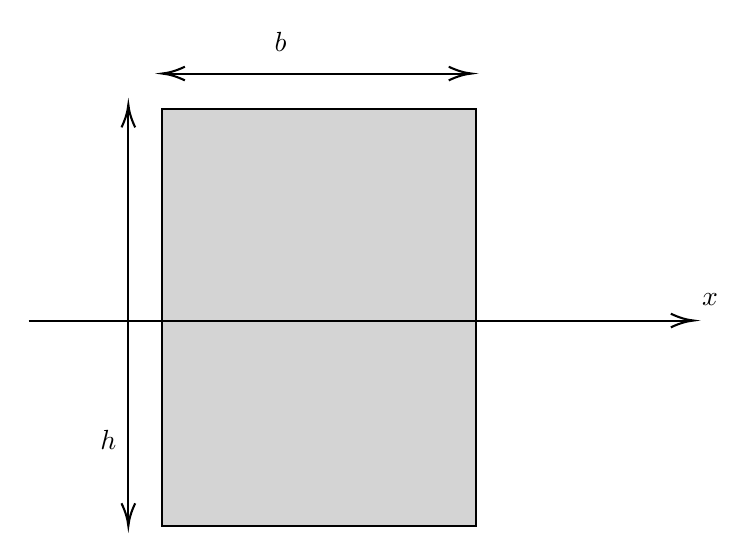
\begin{tikzpicture}[x=0.75pt,y=0.75pt,yscale=-1,xscale=1]
		%uncomment if require: \path (0,428); %set diagram left start at 0, and has height of 428
		
		%Shape: Rectangle [id:dp7076832755710825] 
		\draw  [fill={rgb, 255:red, 212; green, 212; blue, 212 }  ,fill opacity=1 ] (226,65) -- (377.3,65) -- (377.3,266) -- (226,266) -- cycle ;
		%Straight Lines [id:da6197600889391432] 
		\draw    (162,167) -- (480.3,167) ;
		\draw [shift={(482.3,167)}, rotate = 180] [color={rgb, 255:red, 0; green, 0; blue, 0 }  ][line width=0.75]    (10.93,-3.29) .. controls (6.95,-1.4) and (3.31,-0.3) .. (0,0) .. controls (3.31,0.3) and (6.95,1.4) .. (10.93,3.29)   ;
		%Straight Lines [id:da9280821258938541] 
		\draw    (210,65) -- (210,264) ;
		\draw [shift={(210,266)}, rotate = 270] [color={rgb, 255:red, 0; green, 0; blue, 0 }  ][line width=0.75]    (10.93,-3.29) .. controls (6.95,-1.4) and (3.31,-0.3) .. (0,0) .. controls (3.31,0.3) and (6.95,1.4) .. (10.93,3.29)   ;
		\draw [shift={(210,63)}, rotate = 90] [color={rgb, 255:red, 0; green, 0; blue, 0 }  ][line width=0.75]    (10.93,-3.29) .. controls (6.95,-1.4) and (3.31,-0.3) .. (0,0) .. controls (3.31,0.3) and (6.95,1.4) .. (10.93,3.29)   ;
		%Straight Lines [id:da46793955786534447] 
		\draw    (228.3,48) -- (373.3,48) ;
		\draw [shift={(375.3,48)}, rotate = 180] [color={rgb, 255:red, 0; green, 0; blue, 0 }  ][line width=0.75]    (10.93,-3.29) .. controls (6.95,-1.4) and (3.31,-0.3) .. (0,0) .. controls (3.31,0.3) and (6.95,1.4) .. (10.93,3.29)   ;
		\draw [shift={(226.3,48)}, rotate = 0] [color={rgb, 255:red, 0; green, 0; blue, 0 }  ][line width=0.75]    (10.93,-3.29) .. controls (6.95,-1.4) and (3.31,-0.3) .. (0,0) .. controls (3.31,0.3) and (6.95,1.4) .. (10.93,3.29)   ;
		
		% Text Node
		\draw (485,152.4) node [anchor=north west][inner sep=0.75pt]    {$x$};
		% Text Node
		\draw (195,218.4) node [anchor=north west][inner sep=0.75pt]    {$h$};
		% Text Node
		\draw (279,26.4) node [anchor=north west][inner sep=0.75pt]    {$b$};
		
		\end{tikzpicture}
	\end{figure}
	The domain occupied by the plate is given by:
	
	Then we have:
	
	As we will see further below, it is this result that explains why the right one below configuration will have more strength:
	\begin{figure}[H]
		\centering
		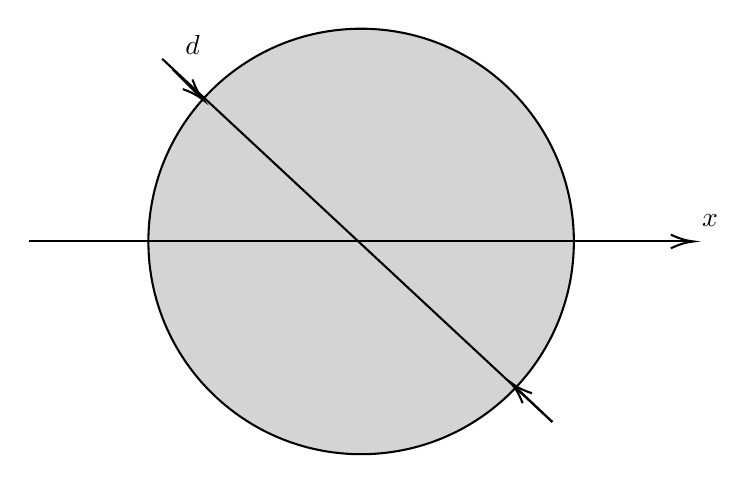
\begin{tikzpicture}[x=0.75pt,y=0.75pt,yscale=-1,xscale=1]
		%uncomment if require: \path (0,428); %set diagram left start at 0, and has height of 428
		
		%Shape: Circle [id:dp018350944667519187] 
		\draw  [fill={rgb, 255:red, 212; green, 212; blue, 212 }  ,fill opacity=1 ] (219.65,167) .. controls (219.65,110.39) and (265.54,64.5) .. (322.15,64.5) .. controls (378.76,64.5) and (424.65,110.39) .. (424.65,167) .. controls (424.65,223.61) and (378.76,269.5) .. (322.15,269.5) .. controls (265.54,269.5) and (219.65,223.61) .. (219.65,167) -- cycle ;
		%Straight Lines [id:da6197600889391432] 
		\draw    (162,167) -- (480.3,167) ;
		\draw [shift={(482.3,167)}, rotate = 180] [color={rgb, 255:red, 0; green, 0; blue, 0 }  ][line width=0.75]    (10.93,-3.29) .. controls (6.95,-1.4) and (3.31,-0.3) .. (0,0) .. controls (3.31,0.3) and (6.95,1.4) .. (10.93,3.29)   ;
		%Straight Lines [id:da9280821258938541] 
		\draw    (414.3,254) -- (226.3,79) ;
		%Straight Lines [id:da46793955786534447] 
		\draw    (395.75,236.38) -- (414.3,254) ;
		\draw [shift={(394.3,235)}, rotate = 43.53] [color={rgb, 255:red, 0; green, 0; blue, 0 }  ][line width=0.75]    (10.93,-3.29) .. controls (6.95,-1.4) and (3.31,-0.3) .. (0,0) .. controls (3.31,0.3) and (6.95,1.4) .. (10.93,3.29)   ;
		%Straight Lines [id:da8679577855526133] 
		\draw    (244.89,97.59) -- (231.3,84) ;
		\draw [shift={(246.3,99)}, rotate = 225] [color={rgb, 255:red, 0; green, 0; blue, 0 }  ][line width=0.75]    (10.93,-3.29) .. controls (6.95,-1.4) and (3.31,-0.3) .. (0,0) .. controls (3.31,0.3) and (6.95,1.4) .. (10.93,3.29)   ;
		
		% Text Node
		\draw (485,152.4) node [anchor=north west][inner sep=0.75pt]    {$x$};
		% Text Node
		\draw (236,66.4) node [anchor=north west][inner sep=0.75pt]    {$d$};
		
		
		\end{tikzpicture}
	\end{figure}
	\pagebreak
	And now let us study the quadratic static moment of a disc of diameter:
	\begin{figure}[H]
		\centering
		% Pattern Info
		\tikzset{
		pattern size/.store in=\mcSize, 
		pattern size = 5pt,
		pattern thickness/.store in=\mcThickness, 
		pattern thickness = 0.3pt,
		pattern radius/.store in=\mcRadius, 
		pattern radius = 1pt}
		\makeatletter
		\pgfutil@ifundefined{pgf@pattern@name@_ly2yqwwqg}{
		\pgfdeclarepatternformonly[\mcThickness,\mcSize]{_ly2yqwwqg}
		{\pgfqpoint{0pt}{0pt}}
		{\pgfpoint{\mcSize+\mcThickness}{\mcSize+\mcThickness}}
		{\pgfpoint{\mcSize}{\mcSize}}
		{
		\pgfsetcolor{\tikz@pattern@color}
		\pgfsetlinewidth{\mcThickness}
		\pgfpathmoveto{\pgfqpoint{0pt}{0pt}}
		\pgfpathlineto{\pgfpoint{\mcSize+\mcThickness}{\mcSize+\mcThickness}}
		\pgfusepath{stroke}
		}}
		\makeatother
		\tikzset{every picture/.style={line width=0.75pt}} %set default line width to 0.75pt        
		
		\begin{tikzpicture}[x=0.75pt,y=0.75pt,yscale=-1,xscale=1]
		%uncomment if require: \path (0,1500); %set diagram left start at 0, and has height of 1500
		
		%Shape: Circle [id:dp5090799602608003] 
		\draw  [pattern=_ly2yqwwqg,pattern size=6pt,pattern thickness=0.75pt,pattern radius=0pt, pattern color={rgb, 255:red, 0; green, 0; blue, 0}][line width=1.5]  (241.73,114.55) .. controls (241.73,79.4) and (270.22,50.91) .. (305.36,50.91) .. controls (340.51,50.91) and (369,79.4) .. (369,114.55) .. controls (369,149.69) and (340.51,178.18) .. (305.36,178.18) .. controls (270.22,178.18) and (241.73,149.69) .. (241.73,114.55) -- cycle ;
		%Straight Lines [id:da6247960411163416] 
		\draw    (205.43,114.55) -- (403.3,114.55) ;
		\draw [shift={(405.3,114.55)}, rotate = 180] [color={rgb, 255:red, 0; green, 0; blue, 0 }  ][line width=0.75]    (10.93,-4.9) .. controls (6.95,-2.3) and (3.31,-0.67) .. (0,0) .. controls (3.31,0.67) and (6.95,2.3) .. (10.93,4.9)   ;
		%Straight Lines [id:da5992618229300815] 
		\draw    (374.86,183.18) -- (234.86,47.18) ;
		%Straight Lines [id:da449420320124547] 
		\draw    (234.86,47.18) -- (255.42,66.8) ;
		\draw [shift={(256.86,68.18)}, rotate = 223.67] [color={rgb, 255:red, 0; green, 0; blue, 0 }  ][line width=0.75]    (10.93,-3.29) .. controls (6.95,-1.4) and (3.31,-0.3) .. (0,0) .. controls (3.31,0.3) and (6.95,1.4) .. (10.93,3.29)   ;
		%Straight Lines [id:da914420635112908] 
		\draw    (374.86,183.18) -- (351.31,160.57) ;
		\draw [shift={(349.86,159.18)}, rotate = 43.83] [color={rgb, 255:red, 0; green, 0; blue, 0 }  ][line width=0.75]    (10.93,-3.29) .. controls (6.95,-1.4) and (3.31,-0.3) .. (0,0) .. controls (3.31,0.3) and (6.95,1.4) .. (10.93,3.29)   ;
		
		% Text Node
		\draw (394,88.31) node [anchor=north west][inner sep=0.75pt]    {$x$};
		% Text Node
		\draw (253,43.31) node [anchor=north west][inner sep=0.75pt]    {$d$};
		\end{tikzpicture}
	\end{figure}
	Here the domain of integration is:
	
	where $d$ is the diameter of the disc.
	
	To calculate this integral, we use polar coordinates that are for recall given by (\SeeChapter{see section Vector Calculus page \pageref{polar coordinates}}):
	
	
	We always have:
	
	
	The Jacobian of the transformation is equal to $r$ (\SeeChapter{see section Differential and Integral Calculus page \pageref{jacobian in polar coordinates}}). We get:
	
	
	Now let us calculate the quadratic static inertia of a ring of external diameter $D$ and internal diameter $d$:
	\begin{figure}[H]
		\centering
		% Pattern Info
		\tikzset{
		pattern size/.store in=\mcSize, 
		pattern size = 5pt,
		pattern thickness/.store in=\mcThickness, 
		pattern thickness = 0.3pt,
		pattern radius/.store in=\mcRadius, 
		pattern radius = 1pt}
		\makeatletter
		\pgfutil@ifundefined{pgf@pattern@name@_d6klexfui}{
		\pgfdeclarepatternformonly[\mcThickness,\mcSize]{_d6klexfui}
		{\pgfqpoint{0pt}{0pt}}
		{\pgfpoint{\mcSize+\mcThickness}{\mcSize+\mcThickness}}
		{\pgfpoint{\mcSize}{\mcSize}}
		{
		\pgfsetcolor{\tikz@pattern@color}
		\pgfsetlinewidth{\mcThickness}
		\pgfpathmoveto{\pgfqpoint{0pt}{0pt}}
		\pgfpathlineto{\pgfpoint{\mcSize+\mcThickness}{\mcSize+\mcThickness}}
		\pgfusepath{stroke}
		}}
		\makeatother
		\tikzset{every picture/.style={line width=0.75pt}} %set default line width to 0.75pt        
		
		\begin{tikzpicture}[x=0.75pt,y=0.75pt,yscale=-1,xscale=1]
		%uncomment if require: \path (0,1500); %set diagram left start at 0, and has height of 1500
		
		%Shape: Circle [id:dp5090799602608003] 
		\draw  [pattern=_d6klexfui,pattern size=6pt,pattern thickness=0.75pt,pattern radius=0pt, pattern color={rgb, 255:red, 0; green, 0; blue, 0}][line width=1.5]  (217.73,115.05) .. controls (217.73,68.58) and (255.4,30.91) .. (301.86,30.91) .. controls (348.33,30.91) and (386,68.58) .. (386,115.05) .. controls (386,161.51) and (348.33,199.18) .. (301.86,199.18) .. controls (255.4,199.18) and (217.73,161.51) .. (217.73,115.05) -- cycle ;
		%Straight Lines [id:da449420320124547] 
		\draw    (221.69,28.31) -- (242.5,50.72) ;
		\draw [shift={(243.86,52.18)}, rotate = 227.11] [color={rgb, 255:red, 0; green, 0; blue, 0 }  ][line width=0.75]    (10.93,-3.29) .. controls (6.95,-1.4) and (3.31,-0.3) .. (0,0) .. controls (3.31,0.3) and (6.95,1.4) .. (10.93,3.29)   ;
		%Straight Lines [id:da914420635112908] 
		\draw    (391.86,207.18) -- (364.25,178.62) ;
		\draw [shift={(362.86,177.18)}, rotate = 45.97] [color={rgb, 255:red, 0; green, 0; blue, 0 }  ][line width=0.75]    (10.93,-3.29) .. controls (6.95,-1.4) and (3.31,-0.3) .. (0,0) .. controls (3.31,0.3) and (6.95,1.4) .. (10.93,3.29)   ;
		%Shape: Circle [id:dp007469558478687022] 
		\draw  [fill={rgb, 255:red, 255; green, 255; blue, 255 }  ,fill opacity=1 ] (239.27,115.05) .. controls (239.27,80.48) and (267.3,52.45) .. (301.86,52.45) .. controls (336.43,52.45) and (364.45,80.48) .. (364.45,115.05) .. controls (364.45,149.61) and (336.43,177.64) .. (301.86,177.64) .. controls (267.3,177.64) and (239.27,149.61) .. (239.27,115.05) -- cycle ;
		%Straight Lines [id:da5992618229300815] 
		\draw    (391.86,207.18) -- (214.86,21.18) ;
		%Straight Lines [id:da6043704477480567] 
		\draw    (261.38,70.45) -- (343.49,156.82) ;
		\draw [shift={(344.86,158.27)}, rotate = 226.45] [color={rgb, 255:red, 0; green, 0; blue, 0 }  ][line width=0.75]    (10.93,-3.29) .. controls (6.95,-1.4) and (3.31,-0.3) .. (0,0) .. controls (3.31,0.3) and (6.95,1.4) .. (10.93,3.29)   ;
		\draw [shift={(260,69)}, rotate = 46.45] [color={rgb, 255:red, 0; green, 0; blue, 0 }  ][line width=0.75]    (10.93,-3.29) .. controls (6.95,-1.4) and (3.31,-0.3) .. (0,0) .. controls (3.31,0.3) and (6.95,1.4) .. (10.93,3.29)   ;
		%Straight Lines [id:da6247960411163416] 
		\draw    (194.86,115.05) -- (411.86,115.05) ;
		\draw [shift={(413.86,115.05)}, rotate = 180] [color={rgb, 255:red, 0; green, 0; blue, 0 }  ][line width=0.75]    (10.93,-4.9) .. controls (6.95,-2.3) and (3.31,-0.67) .. (0,0) .. controls (3.31,0.67) and (6.95,2.3) .. (10.93,4.9)   ;
		%Flowchart: Summing Junction [id:dp09956380123551067] 
		\draw   (298.43,115.18) .. controls (298.43,112.46) and (300.64,110.25) .. (303.36,110.25) .. controls (306.09,110.25) and (308.3,112.46) .. (308.3,115.18) .. controls (308.3,117.91) and (306.09,120.11) .. (303.36,120.11) .. controls (300.64,120.11) and (298.43,117.91) .. (298.43,115.18) -- cycle ; \draw   (299.88,111.69) -- (306.85,118.67) ; \draw   (306.85,111.69) -- (299.88,118.67) ;
		
		% Text Node
		\draw (400,91.31) node [anchor=north west][inner sep=0.75pt]    {$x$};
		% Text Node
		\draw (293,82.31) node [anchor=north west][inner sep=0.75pt]    {$d$};
		% Text Node
		\draw (229,15.4) node [anchor=north west][inner sep=0.75pt]    {$D$};
		\end{tikzpicture}
	\end{figure}
	Here is the domain of integration is:
	
	where $D$ and $d$ are the diameters of the large and small discs.

	If we denote by $S_1$ the domain of the large disc and $S_2$ that of the small disk then:
	
	using the quadratic static moment of inertia of the disk.
	
	For summary, we have therefore:
	
	and finally there exist also the static polar quadratic moment of $S$ with respect to a point O:
	
	It is therefore easy in simple cases to know the static polar moment of inertia and it is very useful for the study of torsion.

	It follows from these tools as more elements of the section are located away from the axis, the more the static quadratic moment will be important and the more (we will prove it just further below) the "arrows" will be weak.
	
	\pagebreak
	\subsubsection{Equation of the elastic line}\label{equation of the elastic line}
	For this case study example, widely used in practice, we will first have to obtain mathematically the geometric form that takes the neutral axis of a beam subjected to bending forces.
	
	\begin{tcolorbox}[title=Remark,arc=10pt,breakable,drop lifted shadow,
  skin=enhanced,
  skin first is subskin of={enhancedfirst}{arc=10pt,no shadow},
  skin middle is subskin of={enhancedmiddle}{arc=10pt,no shadow},
  skin last is subskin of={enhancedlast}{drop lifted shadow}]
	 If all the reactions of a solicited system can be found from the static equilibrium equations, the problem is say to be "\NewTerm{statically determined}\index{statically determined}" or "\NewTerm{isostatic}\index{isostatic}". When the equations of static fail to find the equilibrium of a system, the system is say to be "\NewTerm{hyperstatic}\index{hyperstatic}" or "\NewTerm{statically indeterminate}\index{statically indeterminate}". We also say that while there is "freedom of movement" despite of $n$ connection points, we are in isostatic situation.
	\end{tcolorbox}
	\begin{figure}[H]
		\centering
		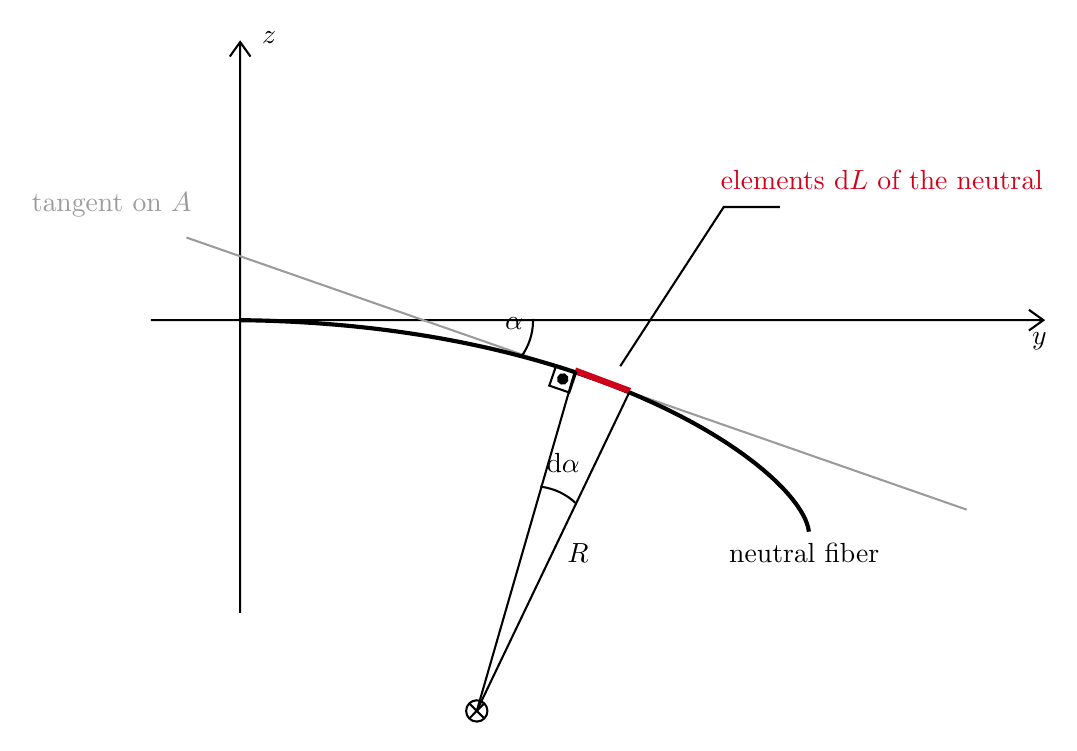
\begin{tikzpicture}[x=0.75pt,y=0.75pt,yscale=-1,xscale=1]
		%uncomment if require: \path (0,1046); %set diagram left start at 0, and has height of 1046
		
		%Shape: Axis 2D [id:dp6289836611638191] 
		\draw  (108.87,194.82) -- (538.87,194.82)(151.87,60.82) -- (151.87,335.82) (531.87,189.82) -- (538.87,194.82) -- (531.87,199.82) (146.87,67.82) -- (151.87,60.82) -- (156.87,67.82)  ;
		%Straight Lines [id:da7788902331081826] 
		\draw [color={rgb, 255:red, 155; green, 155; blue, 155 }  ,draw opacity=1 ]   (126,155) -- (501.87,286.1) ;
		%Curve Lines [id:da35874210672948204] 
		\draw [line width=1.5]    (151.87,194.82) .. controls (327.87,196.73) and (422.87,268.73) .. (425.87,296.73) ;
		%Straight Lines [id:da6190047285433289] 
		\draw [color={rgb, 255:red, 208; green, 2; blue, 27 }  ,draw opacity=1 ][line width=2.25]    (313.23,219.07) -- (339.67,228.94) ;
		%Straight Lines [id:da3405143769105474] 
		\draw    (335,217) -- (384.87,140.28) -- (411.87,140.28) ;
		%Shape: Arc [id:dp6939149626872985] 
		\draw  [draw opacity=0] (292.99,194.23) .. controls (293,194.43) and (293,194.63) .. (293,194.82) .. controls (293,201.49) and (290.83,207.64) .. (287.15,212.62) -- (263,194.82) -- cycle ; \draw   (292.99,194.23) .. controls (293,194.43) and (293,194.63) .. (293,194.82) .. controls (293,201.49) and (290.83,207.64) .. (287.15,212.62) ;  
		%Straight Lines [id:da7244380792826697] 
		\draw    (313.23,219.07) -- (265.87,383.1) ;
		%Straight Lines [id:da491901500606881] 
		\draw    (339.67,228.94) -- (265.87,383.1) ;
		%Flowchart: Summing Junction [id:dp9818431156175802] 
		\draw   (260.74,383.1) .. controls (260.74,380.26) and (263.04,377.96) .. (265.87,377.96) .. controls (268.71,377.96) and (271.01,380.26) .. (271.01,383.1) .. controls (271.01,385.93) and (268.71,388.23) .. (265.87,388.23) .. controls (263.04,388.23) and (260.74,385.93) .. (260.74,383.1) -- cycle ; \draw   (262.24,379.46) -- (269.5,386.73) ; \draw   (269.5,379.46) -- (262.24,386.73) ;
		%Shape: Arc [id:dp8898536077502639] 
		\draw  [draw opacity=0] (296.49,275.03) .. controls (296.69,275.05) and (296.89,275.08) .. (297.08,275.1) .. controls (303.68,276.01) and (309.48,279) .. (313.92,283.32) -- (293,304.82) -- cycle ; \draw   (296.49,275.03) .. controls (296.69,275.05) and (296.89,275.08) .. (297.08,275.1) .. controls (303.68,276.01) and (309.48,279) .. (313.92,283.32) ;  
		%Shape: Rectangle [id:dp6562086129961235] 
		\draw   (304.15,216.65) -- (313.78,219.96) -- (310.45,229.67) -- (300.81,226.36) -- cycle ;
		%Shape: Ellipse [id:dp9241581290061469] 
		\draw  [fill={rgb, 255:red, 0; green, 0; blue, 0 }  ,fill opacity=1 ] (305.15,222.42) .. controls (305.56,221.23) and (306.85,220.59) .. (308.04,221) .. controls (309.22,221.4) and (309.85,222.7) .. (309.44,223.9) .. controls (309.03,225.09) and (307.74,225.73) .. (306.55,225.32) .. controls (305.37,224.92) and (304.74,223.62) .. (305.15,222.42) -- cycle ;
		
		
		% Text Node
		\draw (161,54.4) node [anchor=north west][inner sep=0.75pt]    {$z$};
		% Text Node
		\draw (532,199.4) node [anchor=north west][inner sep=0.75pt]    {$y$};
		% Text Node
		\draw (386,301) node [anchor=north west][inner sep=0.75pt]   [align=left] {neutral fiber};
		% Text Node
		\draw (50,132) node [anchor=north west][inner sep=0.75pt]  [color={rgb, 255:red, 155; green, 155; blue, 155 }  ,opacity=1 ] [align=left] {tangent on $\displaystyle A$};
		% Text Node
		\draw (382,121) node [anchor=north west][inner sep=0.75pt]  [color={rgb, 255:red, 208; green, 2; blue, 27 }  ,opacity=1 ] [align=left] {elements $\displaystyle \mathrm{d} L$ of the neutral};
		% Text Node
		\draw (278,192.22) node [anchor=north west][inner sep=0.75pt]    {$\alpha $};
		% Text Node
		\draw (308,301.13) node [anchor=north west][inner sep=0.75pt]    {$R$};
		% Text Node
		\draw (298,257.22) node [anchor=north west][inner sep=0.75pt]    {$\mathrm{d} \alpha $};
		
		\end{tikzpicture} 
		\vspace*{3mm}
		\caption{Beam (simplified ...) subjected to a force}
	\end{figure}
	By definition of the derivative and under the assumption of small deformations (however that still works well up to $45^\circ$...):
	
	Or by derivating once again:
	
	Moreover, the figure shows that (\SeeChapter{see section Trigonometry page \pageref{spherical trigonometry}}):
	
	But the fact that the neutral fiber curve deviates little from the $y$ axis (small deformations), we can write:
	
	Therefore:
	
	Therefore we can write using the relationships obtained above:
	
	which is the differential equation giving $z=f(y)$, named "\NewTerm{equation of the elastic line}\index{equation of the elastic line}".
	
	Another common but less intuitive approach to get the same relation is to start from:
	
	and to recall that the radius of curvature $R$ is given by (\SeeChapter{see section Differential Geometry page \pageref{radius of curvature}}):
	
	Either by adapting the notation to our context:
	
	and neglecting the first derivative for the small deformations we find indeed:
	
	
	\pagebreak
	\begin{tcolorbox}[colframe=black,colback=white,sharp corners,breakable]
	\textbf{{\Large \ding{45}}Examples:}\\\\
	\textbf{E1.} Cantilevered beam (only at one side) that is classic case in construction and housing) with concentrated load (punctual) at the end:
	\begin{figure}[H]
		\begin{tikzpicture}[x=0.75pt,y=0.75pt,yscale=-1,xscale=1]
		%uncomment if require: \path (0,1467); %set diagram left start at 0, and has height of 1467

		% Pattern Info		 
		\tikzset{
		pattern size/.store in=\mcSize, 
		pattern size = 5pt,
		pattern thickness/.store in=\mcThickness, 
		pattern thickness = 0.3pt,
		pattern radius/.store in=\mcRadius, 
		pattern radius = 1pt}
		\makeatletter
		\pgfutil@ifundefined{pgf@pattern@name@_44axfk68e}{
		\pgfdeclarepatternformonly[\mcThickness,\mcSize]{_44axfk68e}
		{\pgfqpoint{0pt}{0pt}}
		{\pgfpoint{\mcSize+\mcThickness}{\mcSize+\mcThickness}}
		{\pgfpoint{\mcSize}{\mcSize}}
		{
		\pgfsetcolor{\tikz@pattern@color}
		\pgfsetlinewidth{\mcThickness}
		\pgfpathmoveto{\pgfqpoint{0pt}{0pt}}
		\pgfpathlineto{\pgfpoint{\mcSize+\mcThickness}{\mcSize+\mcThickness}}
		\pgfusepath{stroke}
		}}
		
		%Shape: Rectangle [id:dp9822820618549515] 
		\draw  [draw opacity=0][pattern=_44axfk68e,pattern size=8.7pt,pattern thickness=0.75pt,pattern radius=0pt, pattern color={rgb, 255:red, 0; green, 0; blue, 0}] (79,92) -- (177.5,92) -- (177.5,323) -- (79,323) -- cycle ;
		%Straight Lines [id:da1262165090771199] 
		\draw [line width=2.25]    (177.5,92) -- (177.5,323) ;
		%Shape: Square [id:dp7417482285076933] 
		\draw  [fill={rgb, 255:red, 255; green, 255; blue, 255 }  ,fill opacity=1 ][line width=1.5]  (110,158) -- (178,158) -- (178,226) -- (110,226) -- cycle ;
		%Straight Lines [id:da21671293148558313] 
		\draw [color={rgb, 255:red, 255; green, 255; blue, 255 }  ,draw opacity=1 ][line width=2.25]    (178,158) -- (178,224) ;
		%Shape: Polygon Curved [id:ds9160032413571948] 
		\draw  [fill={rgb, 255:red, 255; green, 255; blue, 255 }  ,fill opacity=1 ][line width=1.5]  (178,158) .. controls (177.5,158) and (283.53,155.3) .. (377.5,171) .. controls (471.47,186.7) and (530.5,213) .. (532.5,214) .. controls (534.5,215) and (508.5,278) .. (508.5,277) .. controls (508.5,276) and (445.11,250.54) .. (368.5,238) .. controls (291.89,225.46) and (177.73,225.45) .. (178,226) .. controls (178.27,226.55) and (178.5,158) .. (178,158) -- cycle ;
		%Straight Lines [id:da8917401810189851] 
		\draw  [dash pattern={on 4.5pt off 4.5pt}]  (178,158) -- (554.5,158) ;
		%Straight Lines [id:da9530500092583731] 
		\draw [color={rgb, 255:red, 255; green, 255; blue, 255 }  ,draw opacity=1 ][line width=3]    (178.63,159) -- (178.63,224.75) ;
		%Straight Lines [id:da3774805815324547] 
		\draw  [dash pattern={on 4.5pt off 4.5pt}]  (532.5,214) -- (557.5,214) ;
		%Straight Lines [id:da5462225606770972] 
		\draw    (547,161) -- (547,212) ;
		\draw [shift={(547,214)}, rotate = 270] [color={rgb, 255:red, 0; green, 0; blue, 0 }  ][line width=0.75]    (10.93,-3.29) .. controls (6.95,-1.4) and (3.31,-0.3) .. (0,0) .. controls (3.31,0.3) and (6.95,1.4) .. (10.93,3.29)   ;
		\draw [shift={(547,159)}, rotate = 90] [color={rgb, 255:red, 0; green, 0; blue, 0 }  ][line width=0.75]    (10.93,-3.29) .. controls (6.95,-1.4) and (3.31,-0.3) .. (0,0) .. controls (3.31,0.3) and (6.95,1.4) .. (10.93,3.29)   ;
		%Straight Lines [id:da7303537817294758] 
		\draw    (532.5,110) -- (532.5,214) ;
		%Straight Lines [id:da37669561458937983] 
		\draw    (530.5,124) -- (180.5,124) ;
		\draw [shift={(178.5,124)}, rotate = 360] [color={rgb, 255:red, 0; green, 0; blue, 0 }  ][line width=0.75]    (10.93,-3.29) .. controls (6.95,-1.4) and (3.31,-0.3) .. (0,0) .. controls (3.31,0.3) and (6.95,1.4) .. (10.93,3.29)   ;
		\draw [shift={(532.5,124)}, rotate = 180] [color={rgb, 255:red, 0; green, 0; blue, 0 }  ][line width=0.75]    (10.93,-3.29) .. controls (6.95,-1.4) and (3.31,-0.3) .. (0,0) .. controls (3.31,0.3) and (6.95,1.4) .. (10.93,3.29)   ;
		%Straight Lines [id:da7593311521786705] 
		\draw  [dash pattern={on 0.84pt off 2.51pt}]  (348,140) -- (348,265) ;
		%Straight Lines [id:da2090975024848707] 
		\draw    (343.5,244) -- (179.5,244) ;
		\draw [shift={(177.5,244)}, rotate = 360] [color={rgb, 255:red, 0; green, 0; blue, 0 }  ][line width=0.75]    (10.93,-3.29) .. controls (6.95,-1.4) and (3.31,-0.3) .. (0,0) .. controls (3.31,0.3) and (6.95,1.4) .. (10.93,3.29)   ;
		\draw [shift={(345.5,244)}, rotate = 180] [color={rgb, 255:red, 0; green, 0; blue, 0 }  ][line width=0.75]    (10.93,-3.29) .. controls (6.95,-1.4) and (3.31,-0.3) .. (0,0) .. controls (3.31,0.3) and (6.95,1.4) .. (10.93,3.29)   ;
		%Straight Lines [id:da3042920126009483] 
		\draw [color={rgb, 255:red, 208; green, 2; blue, 27 }  ,draw opacity=1 ][line width=1.5]    (523,244) -- (523,312) ;
		\draw [shift={(523,316)}, rotate = 270] [fill={rgb, 255:red, 208; green, 2; blue, 27 }  ,fill opacity=1 ][line width=0.08]  [draw opacity=0] (11.61,-5.58) -- (0,0) -- (11.61,5.58) -- cycle    ;
		%Shape: Axis 2D [id:dp20233095755404906] 
		\draw  (57,191) -- (605,191)(178,60) -- (178,344) (598,186) -- (605,191) -- (598,196) (173,67) -- (178,60) -- (183,67)  ;
		
		% Text Node
		\draw (161,44.4) node [anchor=north west][inner sep=0.75pt]    {$Z$};
		% Text Node
		\draw (596,201.4) node [anchor=north west][inner sep=0.75pt]    {$Y$};
		% Text Node
		\draw (552,169.4) node [anchor=north west][inner sep=0.75pt]    {$f$};
		% Text Node
		\draw (345,105.4) node [anchor=north west][inner sep=0.75pt]    {$L$};
		% Text Node
		\draw (352,239.4) node [anchor=north west][inner sep=0.75pt]    {$S$};
		% Text Node
		\draw (253,247.4) node [anchor=north west][inner sep=0.75pt]    {$y$};
		% Text Node
		\draw (163,193) node [anchor=north west][inner sep=0.75pt]   [align=left] {O};
		% Text Node
		\draw (526,310.4) node [anchor=north west][inner sep=0.75pt]  [color={rgb, 255:red, 208; green, 2; blue, 27 }  ,opacity=1 ]  {$\vec{F}$};
		\end{tikzpicture}
		\vspace*{3mm}
		\caption{Cantilevered beam with punctual force on extremity}
	\end{figure}
	In the section $S$ at any point, the moment of force (bending) is therefore:
	
	On the other hand:
	
	By eliminating $R$ between these two relations, it remains:
	
	The figure shows that the boundary conditions are:
	
	We get after integration:
	
	Therefore:
	
	If $y=L$ the deformation is maximum and $z$ therefore takes the maximum value $f$ named the "\NewTerm{arrow}\index{arrow (mechanical engineering)}" or \NewTerm{deflection}\index{deflection}" (distance between the top initial position of the cantilever and the top of the final position in the above example). It follows:
	
	This gives us finally the maximum vertical deflection of the end to a beam fixed on one side:
	
	All data from this relation are known to us (force, length, Young's modulus, static momentum) and it is then possible to determine whether the bar will break or not because we simply need to apply the relation proved above:
	
	So thanks to the relation:
	
	and knowing experimentally from what experimental value of $\sigma$ the material breaks down we will know when the beam will also break down (at least approximately!) knowing the arrow $f$, the bending moment $M$ and the static quadratic moment $I$.\\

	So we have a result that will be useful to us later:
	
	and integrating from $0$ to $L$ we find the arrow of our previous beam!\\

	\textbf{E2.} The sustained beam (also named "\NewTerm{beam two times supported}" or "\NewTerm{isostatic beam}\index{isostatic beam}") is the most classic example in construction and therefore architecture (and for those who played during childhood to put wooden slats to move over a small river). This is a homogeneous beam, of constant section, resting on two free bearings at its ends and subjected to a load $F$ at the center:
	\begin{figure}[H]
		\centering	
		\begin{tikzpicture}[x=0.75pt,y=0.75pt,yscale=-1,xscale=1]
		%uncomment if require: \path (0,916); %set diagram left start at 0, and has height of 916
		
		% Pattern Info
		 
		\tikzset{
		pattern size/.store in=\mcSize, 
		pattern size = 5pt,
		pattern thickness/.store in=\mcThickness, 
		pattern thickness = 0.3pt,
		pattern radius/.store in=\mcRadius, 
		pattern radius = 1pt}
		\makeatletter
		\pgfutil@ifundefined{pgf@pattern@name@_88nvlqkrq}{
		\pgfdeclarepatternformonly[\mcThickness,\mcSize]{_88nvlqkrq}
		{\pgfqpoint{0pt}{0pt}}
		{\pgfpoint{\mcSize+\mcThickness}{\mcSize+\mcThickness}}
		{\pgfpoint{\mcSize}{\mcSize}}
		{
		\pgfsetcolor{\tikz@pattern@color}
		\pgfsetlinewidth{\mcThickness}
		\pgfpathmoveto{\pgfqpoint{0pt}{0pt}}
		\pgfpathlineto{\pgfpoint{\mcSize+\mcThickness}{\mcSize+\mcThickness}}
		\pgfusepath{stroke}
		}}
		
		% Pattern Info
		 
		\tikzset{
		pattern size/.store in=\mcSize, 
		pattern size = 5pt,
		pattern thickness/.store in=\mcThickness, 
		pattern thickness = 0.3pt,
		pattern radius/.store in=\mcRadius, 
		pattern radius = 1pt}
		\makeatletter
		\pgfutil@ifundefined{pgf@pattern@name@_fcd6uzdzt}{
		\pgfdeclarepatternformonly[\mcThickness,\mcSize]{_fcd6uzdzt}
		{\pgfqpoint{0pt}{0pt}}
		{\pgfpoint{\mcSize+\mcThickness}{\mcSize+\mcThickness}}
		{\pgfpoint{\mcSize}{\mcSize}}
		{
		\pgfsetcolor{\tikz@pattern@color}
		\pgfsetlinewidth{\mcThickness}
		\pgfpathmoveto{\pgfqpoint{0pt}{0pt}}
		\pgfpathlineto{\pgfpoint{\mcSize+\mcThickness}{\mcSize+\mcThickness}}
		\pgfusepath{stroke}
		}}
		
		%Shape: Rectangle [id:dp6929031911003805] 
		\draw  [draw opacity=0][pattern=_88nvlqkrq,pattern size=7.7250000000000005pt,pattern thickness=0.75pt,pattern radius=0pt, pattern color={rgb, 255:red, 0; green, 0; blue, 0}] (99,167) -- (154,167) -- (154,184) -- (99,184) -- cycle ;
		%Straight Lines [id:da009403808312514306] 
		\draw [line width=2.25]    (99,167) -- (154,167) ;
		%Shape: Rectangle [id:dp48971005608894824] 
		\draw  [draw opacity=0][pattern=_fcd6uzdzt,pattern size=7.7250000000000005pt,pattern thickness=0.75pt,pattern radius=0pt, pattern color={rgb, 255:red, 0; green, 0; blue, 0}] (507,167) -- (562,167) -- (562,184) -- (507,184) -- cycle ;
		%Straight Lines [id:da506026543221715] 
		\draw [line width=2.25]    (507,167) -- (562,167) ;
		%Shape: Triangle [id:dp15641428652164846] 
		\draw  [line width=1.5]  (126,144) -- (142,167) -- (110,167) -- cycle ;
		%Shape: Triangle [id:dp16399079770106062] 
		\draw  [line width=1.5]  (536,144) -- (552,167) -- (520,167) -- cycle ;
		%Straight Lines [id:da006569764108090181] 
		\draw [color={rgb, 255:red, 128; green, 128; blue, 128 }  ,draw opacity=1 ][line width=2.25]    (123,107) -- (115,141) ;
		%Straight Lines [id:da09493909506583642] 
		\draw [color={rgb, 255:red, 128; green, 128; blue, 128 }  ,draw opacity=1 ][line width=2.25]    (535,107) -- (545,141) ;
		%Curve Lines [id:da5954188607148141] 
		\draw [color={rgb, 255:red, 155; green, 155; blue, 155 }  ,draw opacity=1 ][line width=2.25]    (115,141) .. controls (124,144) and (224.66,167.88) .. (328,168) .. controls (431.34,168.12) and (524,146) .. (545,141) ;
		%Shape: Rectangle [id:dp5500787310904403] 
		\draw  [color={rgb, 255:red, 155; green, 155; blue, 155 }  ,draw opacity=1 ][dash pattern={on 4.5pt off 4.5pt}] (115,107) -- (545,107) -- (545,141) -- (115,141) -- cycle ;
		%Straight Lines [id:da44883672016593] 
		\draw [color={rgb, 255:red, 74; green, 144; blue, 226 }  ,draw opacity=1 ][line width=1.5]    (126,144) -- (126,91) ;
		\draw [shift={(126,87)}, rotate = 90] [fill={rgb, 255:red, 74; green, 144; blue, 226 }  ,fill opacity=1 ][line width=0.08]  [draw opacity=0] (11.61,-5.58) -- (0,0) -- (11.61,5.58) -- cycle    ;
		%Straight Lines [id:da8499214239786941] 
		\draw [color={rgb, 255:red, 74; green, 144; blue, 226 }  ,draw opacity=1 ][line width=1.5]    (536,144) -- (536,91) ;
		\draw [shift={(536,87)}, rotate = 90] [fill={rgb, 255:red, 74; green, 144; blue, 226 }  ,fill opacity=1 ][line width=0.08]  [draw opacity=0] (11.61,-5.58) -- (0,0) -- (11.61,5.58) -- cycle    ;
		%Straight Lines [id:da7863982670482035] 
		\draw [color={rgb, 255:red, 208; green, 2; blue, 27 }  ,draw opacity=1 ][line width=1.5]    (328,168) -- (328,278) ;
		\draw [shift={(328,282)}, rotate = 270] [fill={rgb, 255:red, 208; green, 2; blue, 27 }  ,fill opacity=1 ][line width=0.08]  [draw opacity=0] (11.61,-5.58) -- (0,0) -- (11.61,5.58) -- cycle    ;
		%Straight Lines [id:da46752334190622524] 
		\draw    (117,68) -- (542,68) ;
		\draw [shift={(544,68)}, rotate = 180] [color={rgb, 255:red, 0; green, 0; blue, 0 }  ][line width=0.75]    (10.93,-3.29) .. controls (6.95,-1.4) and (3.31,-0.3) .. (0,0) .. controls (3.31,0.3) and (6.95,1.4) .. (10.93,3.29)   ;
		\draw [shift={(115,68)}, rotate = 0] [color={rgb, 255:red, 0; green, 0; blue, 0 }  ][line width=0.75]    (10.93,-3.29) .. controls (6.95,-1.4) and (3.31,-0.3) .. (0,0) .. controls (3.31,0.3) and (6.95,1.4) .. (10.93,3.29)   ;
		%Straight Lines [id:da9879082534638635] 
		\draw    (115,107) -- (115,57) ;
		%Straight Lines [id:da9643407063769167] 
		\draw    (545,107) -- (545,57) ;
		%Curve Lines [id:da85325959510549] 
		\draw [color={rgb, 255:red, 155; green, 155; blue, 155 }  ,draw opacity=1 ][line width=2.25]    (123,107) .. controls (132,110) and (225.66,134.88) .. (329,135) .. controls (432.34,135.12) and (514,112) .. (535,107) ;
		%Straight Lines [id:da5215515485927316] 
		\draw    (328,166) -- (328,145) ;
		\draw [shift={(328,143)}, rotate = 90] [color={rgb, 255:red, 0; green, 0; blue, 0 }  ][line width=0.75]    (10.93,-3.29) .. controls (6.95,-1.4) and (3.31,-0.3) .. (0,0) .. controls (3.31,0.3) and (6.95,1.4) .. (10.93,3.29)   ;
		\draw [shift={(328,168)}, rotate = 270] [color={rgb, 255:red, 0; green, 0; blue, 0 }  ][line width=0.75]    (10.93,-3.29) .. controls (6.95,-1.4) and (3.31,-0.3) .. (0,0) .. controls (3.31,0.3) and (6.95,1.4) .. (10.93,3.29)   ;
		
		% Text Node
		\draw (134,77.9) node [anchor=north west][inner sep=0.75pt]  [color={rgb, 255:red, 74; green, 144; blue, 226 }  ,opacity=1 ]  {$\vec{F} /2$};
		% Text Node
		\draw (497,77.9) node [anchor=north west][inner sep=0.75pt]  [color={rgb, 255:red, 74; green, 144; blue, 226 }  ,opacity=1 ]  {$\vec{F} /2$};
		% Text Node
		\draw (339,247.4) node [anchor=north west][inner sep=0.75pt]  [color={rgb, 255:red, 208; green, 2; blue, 27 }  ,opacity=1 ]  {$\vec{F}$};
		% Text Node
		\draw (321,45.4) node [anchor=north west][inner sep=0.75pt]    {$L$};
		% Text Node
		\draw (336,143.4) node [anchor=north west][inner sep=0.75pt]    {$f$};
		
		\end{tikzpicture}
		\vspace*{3mm}
		\caption{Sustained beam with punctual centered force}
	\end{figure}
	We can therefore consider that it is as if we had $F / 2$ at both ends of two beams of length $L / 2$ (thus the sum is indeed equal to $F$, that is to say, the bending moment). Notice that we neglect the weight of the beam relatively to that of $F$, but $F$ may be simply the weight of the beam! Using the last relation of the previous example, we have:
	
	Therefore:
	
	Thus the maximum vertical deflection of a beam connected on both sides is finally (changing a bit the notation):
	
	Thus, for a same length of beam, at identical $F$ the arrow  is $16$ times smaller than for a fixed beam! It was intuitive that it was lower for the same force but hard to guess that it would be of a factor $16$...!\\

	It is this relationship that is also used for IPN beams (famous beams in building construction!).\\

	\textbf{E3}. Beam built only one side still named "cantilever beam" (also classic case in the construction and housing) but now with a constant line load denoted $w$:
	\begin{figure}[H]
		\centering 
		\begin{tikzpicture}[x=0.75pt,y=0.75pt,yscale=-1,xscale=1]
		%uncomment if require: \path (0,1467); %set diagram left start at 0, and has height of 1467
		
		% Pattern Info
		\tikzset{
		pattern size/.store in=\mcSize, 
		pattern size = 5pt,
		pattern thickness/.store in=\mcThickness, 
		pattern thickness = 0.3pt,
		pattern radius/.store in=\mcRadius, 
		pattern radius = 1pt}
		\makeatletter
		\pgfutil@ifundefined{pgf@pattern@name@_bslb3ktav}{
		\pgfdeclarepatternformonly[\mcThickness,\mcSize]{_bslb3ktav}
		{\pgfqpoint{0pt}{0pt}}
		{\pgfpoint{\mcSize+\mcThickness}{\mcSize+\mcThickness}}
		{\pgfpoint{\mcSize}{\mcSize}}
		{
		\pgfsetcolor{\tikz@pattern@color}
		\pgfsetlinewidth{\mcThickness}
		\pgfpathmoveto{\pgfqpoint{0pt}{0pt}}
		\pgfpathlineto{\pgfpoint{\mcSize+\mcThickness}{\mcSize+\mcThickness}}
		\pgfusepath{stroke}
		}}  
		
		%Shape: Rectangle [id:dp671181491975279] 
		\draw  [draw opacity=0][pattern=_bslb3ktav,pattern size=7.574999999999999pt,pattern thickness=0.75pt,pattern radius=0pt, pattern color={rgb, 255:red, 0; green, 0; blue, 0}] (491,93) -- (609.5,93) -- (609.5,280) -- (491,280) -- cycle ;
		%Straight Lines [id:da7878155762487142] 
		\draw [line width=2.25]    (491,93) -- (491,280) ;
		%Shape: Rectangle [id:dp801361489268243] 
		\draw  [fill={rgb, 255:red, 255; green, 255; blue, 255 }  ,fill opacity=1 ][line width=1.5]  (158,198) -- (531.5,198) -- (531.5,212) -- (158,212) -- cycle ;
		%Straight Lines [id:da7598319727828826] 
		\draw  [dash pattern={on 15pt off 3pt on 3.75pt off 1.5pt}]  (127.5,205) -- (628.5,205) ;
		\draw [shift={(630.5,205)}, rotate = 180] [color={rgb, 255:red, 0; green, 0; blue, 0 }  ][line width=0.75]    (10.93,-4.9) .. controls (6.95,-2.3) and (3.31,-0.67) .. (0,0) .. controls (3.31,0.67) and (6.95,2.3) .. (10.93,4.9)   ;
		%Straight Lines [id:da43315195694002084] 
		\draw [line width=1.5]    (157,105) -- (157,194) ;
		\draw [shift={(157,198)}, rotate = 270] [fill={rgb, 255:red, 0; green, 0; blue, 0 }  ][line width=0.08]  [draw opacity=0] (11.61,-5.58) -- (0,0) -- (11.61,5.58) -- cycle    ;
		%Straight Lines [id:da6486614639381474] 
		\draw [line width=1.5]    (176.29,105) -- (176.29,194) ;
		\draw [shift={(176.29,198)}, rotate = 270] [fill={rgb, 255:red, 0; green, 0; blue, 0 }  ][line width=0.08]  [draw opacity=0] (11.61,-5.58) -- (0,0) -- (11.61,5.58) -- cycle    ;
		%Straight Lines [id:da460799021630554] 
		\draw [line width=1.5]    (195.58,105) -- (195.58,194) ;
		\draw [shift={(195.58,198)}, rotate = 270] [fill={rgb, 255:red, 0; green, 0; blue, 0 }  ][line width=0.08]  [draw opacity=0] (11.61,-5.58) -- (0,0) -- (11.61,5.58) -- cycle    ;
		%Straight Lines [id:da12059025165670523] 
		\draw [line width=1.5]    (214.87,105) -- (214.87,194) ;
		\draw [shift={(214.87,198)}, rotate = 270] [fill={rgb, 255:red, 0; green, 0; blue, 0 }  ][line width=0.08]  [draw opacity=0] (11.61,-5.58) -- (0,0) -- (11.61,5.58) -- cycle    ;
		%Straight Lines [id:da24999024280670668] 
		\draw [line width=1.5]    (234.16,105) -- (234.16,194) ;
		\draw [shift={(234.16,198)}, rotate = 270] [fill={rgb, 255:red, 0; green, 0; blue, 0 }  ][line width=0.08]  [draw opacity=0] (11.61,-5.58) -- (0,0) -- (11.61,5.58) -- cycle    ;
		%Straight Lines [id:da4610276908561344] 
		\draw [line width=1.5]    (253.45,105) -- (253.45,194) ;
		\draw [shift={(253.45,198)}, rotate = 270] [fill={rgb, 255:red, 0; green, 0; blue, 0 }  ][line width=0.08]  [draw opacity=0] (11.61,-5.58) -- (0,0) -- (11.61,5.58) -- cycle    ;
		%Straight Lines [id:da2680211129620145] 
		\draw [line width=1.5]    (272.74,105) -- (272.74,194) ;
		\draw [shift={(272.74,198)}, rotate = 270] [fill={rgb, 255:red, 0; green, 0; blue, 0 }  ][line width=0.08]  [draw opacity=0] (11.61,-5.58) -- (0,0) -- (11.61,5.58) -- cycle    ;
		%Straight Lines [id:da1207788197564541] 
		\draw [line width=1.5]    (292.03,105) -- (292.03,194) ;
		\draw [shift={(292.03,198)}, rotate = 270] [fill={rgb, 255:red, 0; green, 0; blue, 0 }  ][line width=0.08]  [draw opacity=0] (11.61,-5.58) -- (0,0) -- (11.61,5.58) -- cycle    ;
		%Straight Lines [id:da5296593948061372] 
		\draw [line width=1.5]    (311.32,105) -- (311.32,194) ;
		\draw [shift={(311.32,198)}, rotate = 270] [fill={rgb, 255:red, 0; green, 0; blue, 0 }  ][line width=0.08]  [draw opacity=0] (11.61,-5.58) -- (0,0) -- (11.61,5.58) -- cycle    ;
		%Straight Lines [id:da543754159117205] 
		\draw [line width=1.5]    (330.61,105) -- (330.61,194) ;
		\draw [shift={(330.61,198)}, rotate = 270] [fill={rgb, 255:red, 0; green, 0; blue, 0 }  ][line width=0.08]  [draw opacity=0] (11.61,-5.58) -- (0,0) -- (11.61,5.58) -- cycle    ;
		%Straight Lines [id:da7682085968807331] 
		\draw [line width=1.5]    (349.9,105) -- (349.9,194) ;
		\draw [shift={(349.9,198)}, rotate = 270] [fill={rgb, 255:red, 0; green, 0; blue, 0 }  ][line width=0.08]  [draw opacity=0] (11.61,-5.58) -- (0,0) -- (11.61,5.58) -- cycle    ;
		%Straight Lines [id:da22049110750973333] 
		\draw [line width=1.5]    (369.19,105) -- (369.19,194) ;
		\draw [shift={(369.19,198)}, rotate = 270] [fill={rgb, 255:red, 0; green, 0; blue, 0 }  ][line width=0.08]  [draw opacity=0] (11.61,-5.58) -- (0,0) -- (11.61,5.58) -- cycle    ;
		%Straight Lines [id:da7661988452852129] 
		\draw [line width=1.5]    (388.48,105) -- (388.48,194) ;
		\draw [shift={(388.48,198)}, rotate = 270] [fill={rgb, 255:red, 0; green, 0; blue, 0 }  ][line width=0.08]  [draw opacity=0] (11.61,-5.58) -- (0,0) -- (11.61,5.58) -- cycle    ;
		%Straight Lines [id:da7684516993776307] 
		\draw [line width=1.5]    (407.77,105) -- (407.77,194) ;
		\draw [shift={(407.77,198)}, rotate = 270] [fill={rgb, 255:red, 0; green, 0; blue, 0 }  ][line width=0.08]  [draw opacity=0] (11.61,-5.58) -- (0,0) -- (11.61,5.58) -- cycle    ;
		%Straight Lines [id:da3800718047727478] 
		\draw [line width=1.5]    (427.06,105) -- (427.06,194) ;
		\draw [shift={(427.06,198)}, rotate = 270] [fill={rgb, 255:red, 0; green, 0; blue, 0 }  ][line width=0.08]  [draw opacity=0] (11.61,-5.58) -- (0,0) -- (11.61,5.58) -- cycle    ;
		%Straight Lines [id:da16157454841870655] 
		\draw [line width=1.5]    (446.35,105) -- (446.35,194) ;
		\draw [shift={(446.35,198)}, rotate = 270] [fill={rgb, 255:red, 0; green, 0; blue, 0 }  ][line width=0.08]  [draw opacity=0] (11.61,-5.58) -- (0,0) -- (11.61,5.58) -- cycle    ;
		%Straight Lines [id:da5658393531071297] 
		\draw [line width=1.5]    (465.64,105) -- (465.64,194) ;
		\draw [shift={(465.64,198)}, rotate = 270] [fill={rgb, 255:red, 0; green, 0; blue, 0 }  ][line width=0.08]  [draw opacity=0] (11.61,-5.58) -- (0,0) -- (11.61,5.58) -- cycle    ;
		%Straight Lines [id:da6134035493262799] 
		\draw [line width=1.5]    (485,105) -- (485,194) ;
		\draw [shift={(485,198)}, rotate = 270] [fill={rgb, 255:red, 0; green, 0; blue, 0 }  ][line width=0.08]  [draw opacity=0] (11.61,-5.58) -- (0,0) -- (11.61,5.58) -- cycle    ;
		%Straight Lines [id:da20079236385384647] 
		\draw    (157,105) -- (490.5,105) ;
		%Curve Lines [id:da8410429440008431] 
		\draw [line width=1.5]  [dash pattern={on 5.63pt off 4.5pt}]  (162.5,276) .. controls (236.5,225) and (372.5,204) .. (500,205) ;
		%Straight Lines [id:da7993528186588561] 
		\draw    (159,206) -- (159,374) ;
		\draw [shift={(159,376)}, rotate = 270] [color={rgb, 255:red, 0; green, 0; blue, 0 }  ][line width=0.75]    (10.93,-4.9) .. controls (6.95,-2.3) and (3.31,-0.67) .. (0,0) .. controls (3.31,0.67) and (6.95,2.3) .. (10.93,4.9)   ;
		%Straight Lines [id:da44475866967381683] 
		\draw    (143.25,208) -- (143.25,276) ;
		\draw [shift={(143.25,278)}, rotate = 270] [color={rgb, 255:red, 0; green, 0; blue, 0 }  ][line width=0.75]    (10.93,-3.29) .. controls (6.95,-1.4) and (3.31,-0.3) .. (0,0) .. controls (3.31,0.3) and (6.95,1.4) .. (10.93,3.29)   ;
		\draw [shift={(143.25,206)}, rotate = 90] [color={rgb, 255:red, 0; green, 0; blue, 0 }  ][line width=0.75]    (10.93,-3.29) .. controls (6.95,-1.4) and (3.31,-0.3) .. (0,0) .. controls (3.31,0.3) and (6.95,1.4) .. (10.93,3.29)   ;
		%Straight Lines [id:da91639005245582] 
		\draw    (158,278) -- (128.5,278) ;
		%Straight Lines [id:da9480486623770012] 
		\draw    (491,280) -- (491,369) ;
		%Straight Lines [id:da03536541253967207] 
		\draw    (489,344) -- (160.5,344) ;
		\draw [shift={(158.5,344)}, rotate = 360] [color={rgb, 255:red, 0; green, 0; blue, 0 }  ][line width=0.75]    (10.93,-3.29) .. controls (6.95,-1.4) and (3.31,-0.3) .. (0,0) .. controls (3.31,0.3) and (6.95,1.4) .. (10.93,3.29)   ;
		\draw [shift={(491,344)}, rotate = 180] [color={rgb, 255:red, 0; green, 0; blue, 0 }  ][line width=0.75]    (10.93,-3.29) .. controls (6.95,-1.4) and (3.31,-0.3) .. (0,0) .. controls (3.31,0.3) and (6.95,1.4) .. (10.93,3.29)   ;
		%Straight Lines [id:da5054293360780793] 
		\draw    (253.45,198) -- (253.45,317) ;
		%Straight Lines [id:da27558061476902984] 
		\draw    (251.5,302) -- (161.5,302) ;
		\draw [shift={(159.5,302)}, rotate = 360] [color={rgb, 255:red, 0; green, 0; blue, 0 }  ][line width=0.75]    (10.93,-3.29) .. controls (6.95,-1.4) and (3.31,-0.3) .. (0,0) .. controls (3.31,0.3) and (6.95,1.4) .. (10.93,3.29)   ;
		\draw [shift={(253.5,302)}, rotate = 180] [color={rgb, 255:red, 0; green, 0; blue, 0 }  ][line width=0.75]    (10.93,-3.29) .. controls (6.95,-1.4) and (3.31,-0.3) .. (0,0) .. controls (3.31,0.3) and (6.95,1.4) .. (10.93,3.29)   ;
		%Straight Lines [id:da9019640228271257] 
		\draw    (226.5,232) -- (226.5,208) ;
		\draw [shift={(226.5,206)}, rotate = 90] [color={rgb, 255:red, 0; green, 0; blue, 0 }  ][line width=0.75]    (10.93,-3.29) .. controls (6.95,-1.4) and (3.31,-0.3) .. (0,0) .. controls (3.31,0.3) and (6.95,1.4) .. (10.93,3.29)   ;
		\draw [shift={(226.5,234)}, rotate = 270] [color={rgb, 255:red, 0; green, 0; blue, 0 }  ][line width=0.75]    (10.93,-3.29) .. controls (6.95,-1.4) and (3.31,-0.3) .. (0,0) .. controls (3.31,0.3) and (6.95,1.4) .. (10.93,3.29)   ;
		%Straight Lines [id:da521166905765968] 
		\draw    (253.5,236) -- (218.5,236) ;
		
		% Text Node
		\draw (618,217.4) node [anchor=north west][inner sep=0.75pt]    {$X$};
		% Text Node
		\draw (303,79.4) node [anchor=north west][inner sep=0.75pt]    {$q=c^{te}$};
		% Text Node
		\draw  [color={rgb, 255:red, 255; green, 255; blue, 255 }  ,draw opacity=1 ][fill={rgb, 255:red, 255; green, 255; blue, 255 }  ,fill opacity=1 ]  (305,156) -- (358,156) -- (358,182) -- (305,182) -- cycle  ;
		\draw (308,160.4) node [anchor=north west][inner sep=0.75pt]    {$I=c^{te}$};
		% Text Node
		\draw (151,382.4) node [anchor=north west][inner sep=0.75pt]    {$Y$};
		% Text Node
		\draw (134,181) node [anchor=north west][inner sep=0.75pt]   [align=left] {O};
		% Text Node
		\draw (125,233.4) node [anchor=north west][inner sep=0.75pt]    {$f$};
		% Text Node
		\draw (326,326.4) node [anchor=north west][inner sep=0.75pt]    {$L$};
		% Text Node
		\draw (204,284.4) node [anchor=north west][inner sep=0.75pt]    {$x$};
		% Text Node
		\draw (198,215.4) node [anchor=north west][inner sep=0.75pt]    {$\Delta y$};
		\end{tikzpicture}
		\vspace*{3mm}
		\caption{Beam fixed on one side with constant line load}
	\end{figure}
	The development is simple but some simplifications are smart to get at the end an elegant result. So we always start from the equation of the elastic line by adopting the notations relatively to the selected configuration (see figure above):
	
	Thus explicitly:
	
		As the moment of force $M$ is zero at $x = 0$, we have the constant that is zero. Since then:
	
	Integrating again, we get:
	
	As for $x=L$ by hypothesis the deformation is zero, we have then the constant that is given by:
	
	Therefore:
	
	By integrating a last time:
	
	And as on $x=L$ we have $y$ that is also zero, it comes for the constant:
	
	Therefore:
	
	And as the arrow is anyway on $x=0$, we have then:
	
	\end{tcolorbox}
	
	\paragraph{Euler-Bernoulli Beam equation}\mbox{}\\\\
	Let us now consider the case of a beam fixed on both sides (case even more common that the three previous examples!). The analysis will be a bit more difficult and we will have to introduce several new concepts.

	A beam in practice must withstand at least the following efforts:
	\begin{itemize}
		\item Unloaded (normal):
		\begin{center}
		% BLOCK - NORMAL (Unloaded)
		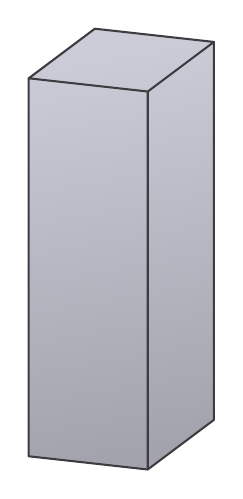
\begin{tikzpicture}[x={(0.72cm,-0.08cm)},y={(0.40cm,0.30cm)},z={(0,1cm)},scale=3]
		\colorlet{metalcol}{blue!25!black!20!white}
		\tikzstyle{metal}=[draw=metalcol!30!black,rounded corners=0.1,top color=metalcol,bottom color=metalcol!80!black,shading angle=10]
		\tikzstyle{force}=[->,red!65!black]
		\def\W{0.7}     % side width
		\def\H{1.6}     % total height
		\def\F{0.28*\H} % force magnitude
		  \draw[metal]
		    (0,0,0) --++ (\W,0,0) --++ (0,0,\H) --++ (-\W,0,0) -- cycle
		    (\W,0,0) --++ (0,\W,0) --++ (0,0,\H) --++ (0,-\W,0) -- cycle
		    (0,0,\H) --++ (\W,0,0) --++ (0,\W,0) --++ (-\W,0,0) -- cycle;
		\end{tikzpicture}
		\end{center}
		
		\item Tension:
		\begin{center}
		% BLOCK - TENSION
		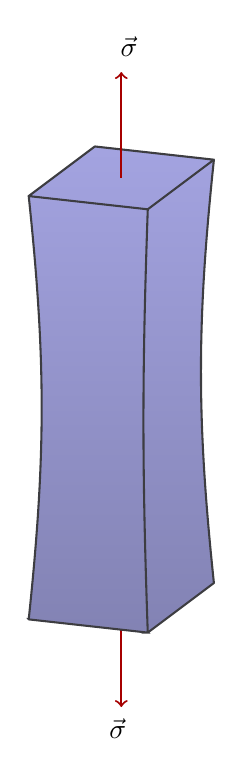
\begin{tikzpicture}[x={(0.72cm,-0.08cm)},y={(0.40cm,0.30cm)},z={(0,1cm)},scale=3]
		\colorlet{metalcol}{blue!25!black!20!white}
		\tikzstyle{metal}=[draw=metalcol!30!black,rounded corners=0.1,top color=metalcol,bottom color=metalcol!80!black,shading angle=10]
		\tikzstyle{force}=[->,red!65!black]
		\def\W{0.7}     % side width
		\def\H{1.6}     % total height
		\def\F{0.28*\H} % force magnitude
		  \def\h{1.12*\H}
		  \draw[force] (\W/2,\W/2,0) --++ (0,0,-\F);
		  \node[below=0pt,left=0pt] at (-3.3,7.2) {$\vec{\sigma}$};
		  \node[below=0pt,left=0pt] at (1.3,-1.2) {$\vec{\sigma}$};
		  \draw[metal,top color=metalcol!80!blue,bottom color=metalcol!80!blue!80!black]
		    (0,0,0) --++ (\W,0,0) to[out=92,in=-92]++ (0,0,\h) --++ (-\W,0,0) to[out=-84,in=84] cycle
		    (\W,0,0) --++ (0,\W,0) to[out=96,in=-96]++ (0,0,\h) --++ (0,-\W,0) to[out=-92,in=92] cycle
		    (0,0,\h) --++ (\W,0,0) --++ (0,\W,0) --++ (-\W,0,0) -- cycle;
		  \draw[force] (\W/2,\W/2,\h) --++ (0,0,\F);
		\end{tikzpicture}
		\end{center}
		
		\item Compression:
		\begin{center}
		% BLOCK - COMPRESSION
		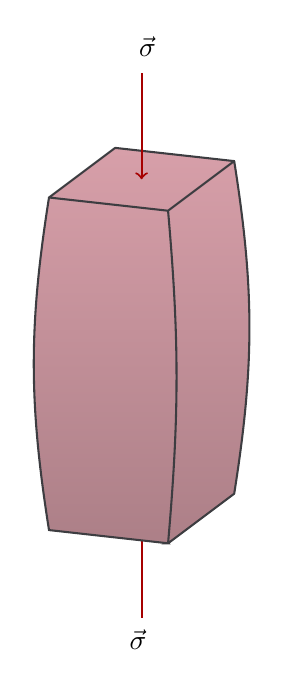
\begin{tikzpicture}[x={(0.72cm,-0.08cm)},y={(0.40cm,0.30cm)},z={(0,1cm)},scale=3]
		\colorlet{metalcol}{blue!25!black!20!white}
		\tikzstyle{metal}=[draw=metalcol!30!black,rounded corners=0.1,top color=metalcol,bottom color=metalcol!80!black,shading angle=10]
		\tikzstyle{force}=[->,red!65!black]
		\def\W{0.7}     % side width
		\def\H{1.6}     % total height
		\def\F{0.28*\H} % force magnitude
		  \def\h{0.88*\H}
		  \draw[force] (\W/2,\W/2,-\F) --++ (0,0,\F);
		  \node[below=0pt,left=0pt] at (-2.7,6.1) {$\vec{\sigma}$};
		  \node[below=0pt,left=0pt] at (1.3,-1.2) {$\vec{\sigma}$};
		  \draw[metal,top color=metalcol!78!red,bottom color=metalcol!78!red!80!black]
		    (0,0,0) --++ (\W,0,0) to[out=85,in=-85]++ (0,0,\h) --++ (-\W,0,0) to[out=-99,in=99] cycle
		    (\W,0,0) --++ (0,\W,0) to[out=81,in=-81]++ (0,0,\h) --++ (0,-\W,0) to[out=-85,in=85] cycle
		    (0,0,\h) --++ (\W,0,0) --++ (0,\W,0) --++ (-\W,0,0) -- cycle;
		  \draw[force] (\W/2,\W/2,\h+\F) --++ (0,0,-\F);
		\end{tikzpicture}
		\end{center}
		
		\item Shearing (shear):
		\begin{center}
		% BLOCK - SHEAR
		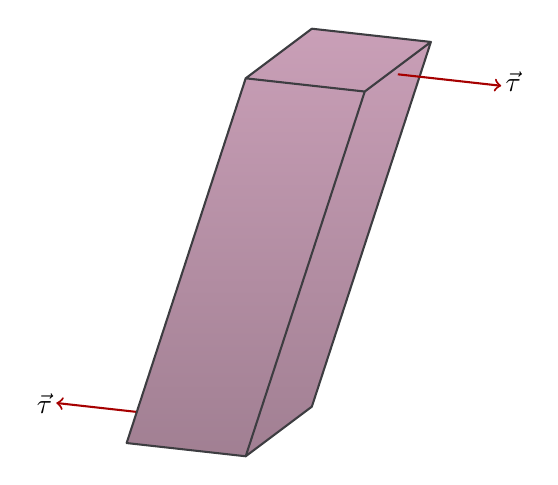
\begin{tikzpicture}[x={(0.72cm,-0.08cm)},y={(0.40cm,0.30cm)},z={(0,1cm)},scale=3]
		\colorlet{metalcol}{blue!25!black!20!white}
		\tikzstyle{metal}=[draw=metalcol!30!black,rounded corners=0.1,top color=metalcol,bottom color=metalcol!80!black,shading angle=10]
		\tikzstyle{force}=[->,red!65!black]
		\def\W{0.7}     % side width
		\def\H{1.6}     % total height
		\def\F{0.28*\H} % force magnitude
		  \def\dw{\W}
		  \def\F{0.38*\H} % force magnitude
		  \draw[force] (0,\W/2,0.01*\H) --++ (-\F,0,0);
		  %top right force legend
		  \node[below=0pt,left=0pt] at (-0.4,5) {$\vec{\tau}$};
		  \draw[metal,top color=metalcol!78!purple,bottom color=metalcol!78!purple!80!black]
		    (0,0,0) --++ (\W,0,0) --++ (\dw,0,\H) --++ (-\W,0,0) -- cycle
		    (\W,0,0) --++ (0,\W,0) --++ (\dw,0,\H) --++ (0,-\W,0) -- cycle
		    (\dw,0,\H) --++ (\W,0,0) --++ (0,\W,0) --++ (-\W,0,0) -- cycle;
		  \draw[force] (\W+\dw,\W/2,0.98*\H) --++ (\F,0,0);
		  \node[below=0pt,left=0pt] at (-0.6,0.4) {$\vec{\tau}$};
		\end{tikzpicture}
		\end{center}

		\item Flexion (bending stress):
		\begin{center}
		% BLOCK - BENDING (flexion)
		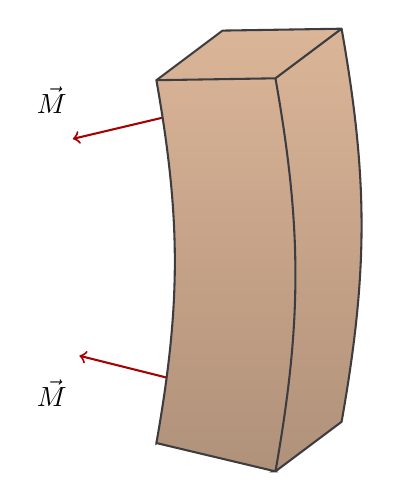
\begin{tikzpicture}[x={(0.72cm,-0.08cm)},y={(0.40cm,0.30cm)},z={(0,1cm)},scale=3]
		\colorlet{metalcol}{blue!25!black!20!white}
		\tikzstyle{metal}=[draw=metalcol!30!black,rounded corners=0.1,top color=metalcol,bottom color=metalcol!80!black,shading angle=10]
		\tikzstyle{force}=[->,red!65!black]
		\def\W{0.7}     % side width
		\def\H{1.6}     % total height
		\def\F{0.28*\H} % force magnitude
		  \def\F{0.38*\H} % force magnitude
		  \def\dh{0.02*\H}
		  \draw[force] (0,0.3*\W,0.85*\H) --++ (-\F,0,-0.25*\F);
		  \node[below=0pt,left=0pt] at (-2.8,4.2) {$\vec{M}$};
		  \draw[force] (0,0.4*\W,0.13*\H) --++ (-\F,0, 0.10*\F);
		  \node[below=0pt,left=0pt] at (-0.8,0.6) {$\vec{M}$};
		  \draw[metal,top color=metalcol!70!orange,bottom color=metalcol!70!orange!80!black]
		    (0,0,\dh) -- (\W,0,-\dh) to[out=80,in=-80] (\W,0,\H+\dh) -- (0,0,\H-\dh) to[out=-80,in=80] cycle
		    (\W,0,-\dh) -- (\W,\W,-\dh) to[out=80,in=-80] (\W,\W,\H+\dh) -- (\W,0,\H+\dh) to[out=-80,in=80] cycle
		    (0,0,\H-\dh) -- (\W,0,\H+\dh) -- (\W,\W,\H+\dh) -- (0,\W,\H-\dh) -- cycle;
		\end{tikzpicture}
		\end{center}
		
		\item Torsion:
		\begin{center}
		% BLOCK - TORSION
		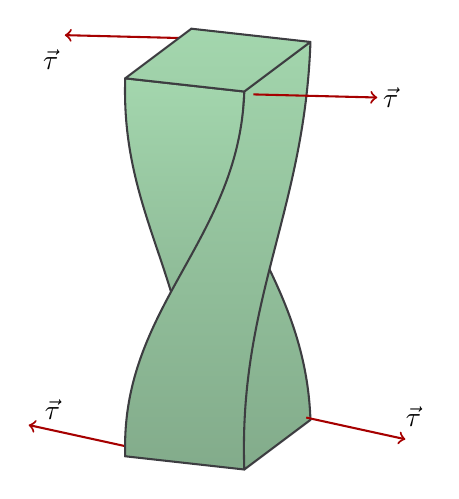
\begin{tikzpicture}[x={(0.72cm,-0.08cm)},y={(0.40cm,0.30cm)},z={(0,1cm)},scale=3]
		\colorlet{metalcol}{blue!25!black!20!white}
		\tikzstyle{metal}=[draw=metalcol!30!black,rounded corners=0.1,top color=metalcol,bottom color=metalcol!80!black,shading angle=10]
		\tikzstyle{force}=[->,red!65!black]
		\def\W{0.7}     % side width
		\def\H{1.6}     % total height
		\def\F{0.28*\H} % force magnitude
		  \def\F{0.41*\H} % force magnitude
		  \draw[force] (0,0.04*\W,0.02*\H) --++ (-\F, 0.2*\F,0);
		  %bottom left force legend
		  \node[below=0pt,left=0pt] at (-0.6,0.5) {$\vec{\tau}$};
		  \draw[force] (0,0.96*\W,0.98*\H) --++ (-\F,-0.2*\F,0);
		  %top left force legend
		  \node[below=0pt,left=0pt] at (-3,4.8) {$\vec{\tau}$};
		  \draw[metal,top color=metalcol!80!green,bottom color=metalcol!80!green!80!black]
		    (\W,0,0) --++ (0,\W,0) to[out=92,in=-92]++ (-\W,0,\H) -- cycle;
		  \draw[metal,top color=metalcol!80!green,bottom color=metalcol!80!green!80!black]
		    (0,\W,0) to[out=92,in=-92]++ (0,-\W,\H) --++ (\W,0,0) to[out=-92,in=90] cycle;
		  \draw[metal,top color=metalcol!80!green,bottom color=metalcol!80!green!80!black]
		    (0,0,0) --++ (\W,0,0) to[out=92,in=-92]++ (0,\W,\H) --++ (0,-\W,0) to[out=-92,in=92] cycle
		    (0,0,\H) --++ (\W,0,0) --++ (0,\W,0) --++ (-\W,0,0) -- cycle;
		  \draw[force] (1.02*\W,0.10*\W,0.98*\H) --++ (\F, 0.2*\F,0);
		  %top right force legend
		  \node[below=0pt,left=0pt] at (-1,4.8) {$\vec{\tau}$};
		  \draw[force] (1.02*\W,0.90*\W,0.02*\H) --++ (\F,-0.2*\F,0);
		  %bottom right legend
		  \node[below=0pt,left=0pt] at (1.3,0.9) {$\vec{\tau}$};
		\end{tikzpicture}
		\end{center}
	\end{itemize}
	Or to summarize in a single figure:
	\begin{figure}[H]
    \colorlet{metalcol}{blue!25!black!20!white}
    \tikzstyle{metal}=[draw=metalcol!30!black,rounded corners=0.1,top color=metalcol,bottom color=metalcol!80!black,shading angle=10]
    \tikzstyle{force}=[->,red!65!black]
    \def\W{0.7}     % side width
    \def\H{1.6}     % total height
    \def\F{0.28*\H} % force magnitude
    
    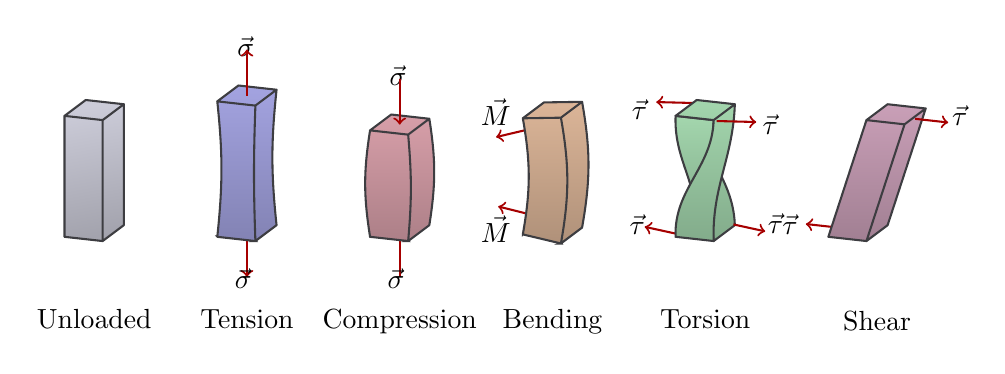
\begin{tikzpicture}[scale=0.96,x={(0.72cm,-0.08cm)},y={(0.40cm,0.30cm)},z={(0,1cm)}]
        % BLOCK - NORMAL (Unloaded)
        \draw[metal]
                (0,0,0) --++ (\W,0,0) --++ (0,0,\H) --++ (-\W,0,0) -- cycle
                (\W,0,0) --++ (0,\W,0) --++ (0,0,\H) --++ (0,-\W,0) -- cycle
                (0,0,\H) --++ (\W,0,0) --++ (0,\W,0) --++ (-\W,0,0) -- cycle;
        
        \node[anchor=center] at (\W/2,\W/2,-1.2){Unloaded\vphantom{p}};
        
        
        % BLOCK - TENSION
        \begin{scope}[xshift=1/6*\textwidth]
                \def\h{1.12*\H}
                \draw[force] (\W/2,\W/2,0) --++ (0,0,-\F);
                \node[below=0pt,left=0pt] at (-3.3,7.5) {$\vec{\sigma}$};
            \node[below=0pt,left=0pt] at (1.6,-1.4) {$\vec{\sigma}$};
            \draw[metal,top color=metalcol!80!blue,bottom color=metalcol!80!blue!80!black]
                (0,0,0) --++ (\W,0,0) to[out=92,in=-92]++ (0,0,\h) --++ (-\W,0,0) to[out=-84,in=84] cycle
                    (\W,0,0) --++ (0,\W,0) to[out=96,in=-96]++ (0,0,\h) --++ (0,-\W,0) to[out=-92,in=92] cycle
                    (0,0,\h) --++ (\W,0,0) --++ (0,\W,0) --++ (-\W,0,0) -- cycle;
            \draw[force] (\W/2,\W/2,\h) --++ (0,0,\F);
              
            \node[anchor=center] at (\W/2,\W/2,-1.2){Tension\vphantom{p}};
        \end{scope}        


        % BLOCK - COMPRESSION
        \begin{scope}[xshift=2/6*\textwidth]
            \def\h{0.88*\H}
                \draw[force] (\W/2,\W/2,-\F) --++ (0,0,\F);
                \node[below=0pt,left=0pt] at (-2.7,6.4) {$\vec{\sigma}$};
                \node[below=0pt,left=0pt] at (1.6,-1.4) {$\vec{\sigma}$};
                \draw[metal,top color=metalcol!78!red,bottom color=metalcol!78!red!80!black]
                    (0,0,0) --++ (\W,0,0) to[out=85,in=-85]++ (0,0,\h) --++ (-\W,0,0) to[out=-99,in=99] cycle
                    (\W,0,0) --++ (0,\W,0) to[out=81,in=-81]++ (0,0,\h) --++ (0,-\W,0) to[out=-85,in=85] cycle
                    (0,0,\h) --++ (\W,0,0) --++ (0,\W,0) --++ (-\W,0,0) -- cycle;
            \draw[force] (\W/2,\W/2,\h+\F) --++ (0,0,-\F);
            
            \node[anchor=center] at (\W/2,\W/2,-1.2){Compression};
        \end{scope}
        
        
        % BLOCK - BENDING (flexion)
        \begin{scope}[xshift=3/6*\textwidth]
            \def\F{0.38*\H} % force magnitude
                \def\dh{0.02*\H}
                \draw[force] (0,0.3*\W,0.85*\H) --++ (-\F,0,-0.25*\F);
                \node[below=0pt,left=0pt] at (-2.7,4.8) {$\vec{M}$};
                \draw[force] (0,0.4*\W,0.13*\H) --++ (-\F,0, 0.10*\F);
            \node[below=0pt,left=0pt] at (-0.2,0.3) {$\vec{M}$};
            \draw[metal,top color=metalcol!70!orange,bottom color=metalcol!70!orange!80!black]
                    (0,0,\dh) -- (\W,0,-\dh) to[out=80,in=-80] (\W,0,\H+\dh) -- (0,0,\H-\dh) to[out=-80,in=80] cycle
                    (\W,0,-\dh) -- (\W,\W,-\dh) to[out=80,in=-80] (\W,\W,\H+\dh) -- (\W,0,\H+\dh) to[out=-80,in=80] cycle
                    (0,0,\H-\dh) -- (\W,0,\H+\dh) -- (\W,\W,\H+\dh) -- (0,\W,\H-\dh) -- cycle;
                    
            \node[anchor=center] at (\W/2,\W/2,-1.2){Bending};
        \end{scope}
        
        
        % BLOCK - TORSION
        \begin{scope}[xshift=4/6*\textwidth]
            \def\F{0.41*\H} % force magnitude
            \draw[force] (0,0.04*\W,0.02*\H) --++ (-\F, 0.2*\F,0);
                \node[below=0pt,left=0pt] at (-0.6,0.4) {$\vec{\tau}$};
            \draw[force] (0,0.96*\W,0.98*\H) --++ (-\F,-0.2*\F,0);
            \node[below=0pt,left=0pt] at (-3,4.8) {$\vec{\tau}$};
            \draw[metal,top color=metalcol!80!green,bottom color=metalcol!80!green!80!black]
                    (\W,0,0) --++ (0,\W,0) to[out=92,in=-92]++ (-\W,0,\H) -- cycle;
            \draw[metal,top color=metalcol!80!green,bottom color=metalcol!80!green!80!black]
                    (0,\W,0) to[out=92,in=-92]++ (0,-\W,\H) --++ (\W,0,0) to[out=-92,in=90] cycle;
                \draw[metal,top color=metalcol!80!green,bottom color=metalcol!80!green!80!black]
                (0,0,0) --++ (\W,0,0) to[out=92,in=-92]++ (0,\W,\H) --++ (0,-\W,0) to[out=-92,in=92] cycle
                (0,0,\H) --++ (\W,0,0) --++ (0,\W,0) --++ (-\W,0,0) -- cycle;
                \draw[force] (1.02*\W,0.10*\W,0.98*\H) --++ (\F, 0.2*\F,0);
                \node[below=0pt,left=0pt] at (-0.6,4.8) {$\vec{\tau}$};
                \draw[force] (1.02*\W,0.90*\W,0.02*\H) --++ (\F,-0.2*\F,0);
            \node[below=0pt,left=0pt] at (1.61,1) {$\vec{\tau}$};
            
            \node[anchor=center] at (\W/2,\W/2,-1.2){Torsion\vphantom{p}};
        \end{scope}
        
        
        % BLOCK - SHEAR
        \begin{scope}[xshift=5/6*\textwidth]
            \def\dw{\W}
            \def\F{0.38*\H} % force magnitude
            \draw[force] (0,\W/2,0.01*\H) --++ (-\F,0,0);
                \node[below=0pt,left=0pt] at (-0.2,5.3) {$\vec{\tau}$};
            \draw[metal,top color=metalcol!78!purple,bottom color=metalcol!78!purple!80!black]
                    (0,0,0) --++ (\W,0,0) --++ (\dw,0,\H) --++ (-\W,0,0) -- cycle
                    (\W,0,0) --++ (0,\W,0) --++ (\dw,0,\H) --++ (0,-\W,0) -- cycle
                    (\dw,0,\H) --++ (\W,0,0) --++ (0,\W,0) --++ (-\W,0,0) -- cycle;
                \draw[force] (\W+\dw,\W/2,0.98*\H) --++ (\F,0,0);
                \node[below=0pt,left=0pt] at (-0.6,0.4) {$\vec{\tau}$};
            
            \node[anchor=center] at (\W/2+\dw/2,\W/2,-1.2){Shear\vphantom{p}};
        \end{scope}
    \end{tikzpicture}   
    \vspace*{3mm}
    \caption[Most common types of material deformations]{Most common types of material deformations (author: Izaak Neutelings)}
    \end{figure}
	If a beam is in equilibrium, then the internal forces must satisfy at all points the following relations:
	
	Let us consider now a beam embedded at its two ends (dual-embedded beam) and let us take in a slice of infinitesimal length $\mathrm{d}y$ such that locally its curvature is zero. The beam will be assumed to be subjected to a uniform force over its entire length (a force which can also be assimilated to its own weight, as already mentioned above). It is then customary to denote by $\vec{w}$ the force per unit length (total weight divided by the length) which is obviously a linear load:
	\begin{figure}[H]
		\centering
		\includegraphics[scale=0.9]{img/engineering/bernoulli_beam_equation.pdf}
	\end{figure}
	If the beam is at equilibrium once deformed (weakly or strongly deformed, this does not matters !) then the sums of the forces of tension, compression, shear and bending must be zero at each point as we have already said! This does not however mean that at each point of the elastic line the values of each of the forces is equal! On the contrary! There are of course differences (if not, there would be no deformation...!).

	Let us first sum the local forces of tension and compression (horizontal) of the element of length $\mathrm{d}y$. We then have schematically:
	\begin{figure}[H]
		\centering
		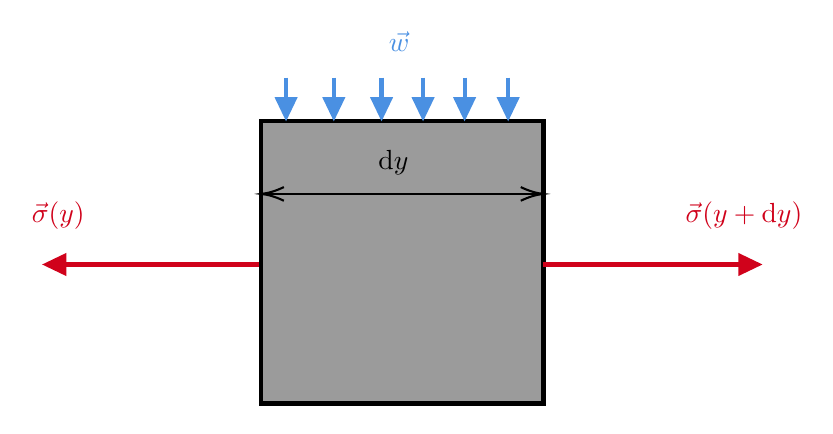
\begin{tikzpicture}[x=0.75pt,y=0.75pt,yscale=-1,xscale=1]
		%uncomment if require: \path (0,1215); %set diagram left start at 0, and has height of 1215
		
		%Shape: Square [id:dp915021229735101] 
		\draw  [fill={rgb, 255:red, 155; green, 155; blue, 155 }  ,fill opacity=1 ][line width=1.5]  (251,80) -- (387,80) -- (387,216) -- (251,216) -- cycle ;
		%Straight Lines [id:da3954525570777263] 
		\draw [color={rgb, 255:red, 208; green, 2; blue, 27 }  ,draw opacity=1 ][line width=1.5]    (250,149) -- (149.5,149) ;
		\draw [shift={(145.5,149)}, rotate = 360] [fill={rgb, 255:red, 208; green, 2; blue, 27 }  ,fill opacity=1 ][line width=0.08]  [draw opacity=0] (11.61,-5.58) -- (0,0) -- (11.61,5.58) -- cycle    ;
		%Straight Lines [id:da1467450967819428] 
		\draw [color={rgb, 255:red, 208; green, 2; blue, 27 }  ,draw opacity=1 ][line width=1.5]    (387,149) -- (488.5,149) ;
		\draw [shift={(492.5,149)}, rotate = 180] [fill={rgb, 255:red, 208; green, 2; blue, 27 }  ,fill opacity=1 ][line width=0.08]  [draw opacity=0] (11.61,-5.58) -- (0,0) -- (11.61,5.58) -- cycle    ;
		%Straight Lines [id:da04551856417568456] 
		\draw    (253,115) -- (385,115) ;
		\draw [shift={(387,115)}, rotate = 180] [color={rgb, 255:red, 0; green, 0; blue, 0 }  ][line width=0.75]    (10.93,-3.29) .. controls (6.95,-1.4) and (3.31,-0.3) .. (0,0) .. controls (3.31,0.3) and (6.95,1.4) .. (10.93,3.29)   ;
		\draw [shift={(251,115)}, rotate = 0] [color={rgb, 255:red, 0; green, 0; blue, 0 }  ][line width=0.75]    (10.93,-3.29) .. controls (6.95,-1.4) and (3.31,-0.3) .. (0,0) .. controls (3.31,0.3) and (6.95,1.4) .. (10.93,3.29)   ;
		%Straight Lines [id:da2605415787168175] 
		\draw [color={rgb, 255:red, 74; green, 144; blue, 226 }  ,draw opacity=1 ][line width=1.5]    (263,59) -- (263,76) ;
		\draw [shift={(263,80)}, rotate = 270] [fill={rgb, 255:red, 74; green, 144; blue, 226 }  ,fill opacity=1 ][line width=0.08]  [draw opacity=0] (11.61,-5.58) -- (0,0) -- (11.61,5.58) -- cycle    ;
		%Straight Lines [id:da3250672832580852] 
		\draw [color={rgb, 255:red, 74; green, 144; blue, 226 }  ,draw opacity=1 ][line width=1.5]    (286,59) -- (286,76) ;
		\draw [shift={(286,80)}, rotate = 270] [fill={rgb, 255:red, 74; green, 144; blue, 226 }  ,fill opacity=1 ][line width=0.08]  [draw opacity=0] (11.61,-5.58) -- (0,0) -- (11.61,5.58) -- cycle    ;
		%Straight Lines [id:da8483440483141562] 
		\draw [color={rgb, 255:red, 74; green, 144; blue, 226 }  ,draw opacity=1 ][line width=1.5]    (309,59) -- (309,76) ;
		\draw [shift={(309,80)}, rotate = 270] [fill={rgb, 255:red, 74; green, 144; blue, 226 }  ,fill opacity=1 ][line width=0.08]  [draw opacity=0] (11.61,-5.58) -- (0,0) -- (11.61,5.58) -- cycle    ;
		%Straight Lines [id:da8903474014081705] 
		\draw [color={rgb, 255:red, 74; green, 144; blue, 226 }  ,draw opacity=1 ][line width=1.5]    (329,59) -- (329,76) ;
		\draw [shift={(329,80)}, rotate = 270] [fill={rgb, 255:red, 74; green, 144; blue, 226 }  ,fill opacity=1 ][line width=0.08]  [draw opacity=0] (11.61,-5.58) -- (0,0) -- (11.61,5.58) -- cycle    ;
		%Straight Lines [id:da7258572747379872] 
		\draw [color={rgb, 255:red, 74; green, 144; blue, 226 }  ,draw opacity=1 ][line width=1.5]    (349,59) -- (349,76) ;
		\draw [shift={(349,80)}, rotate = 270] [fill={rgb, 255:red, 74; green, 144; blue, 226 }  ,fill opacity=1 ][line width=0.08]  [draw opacity=0] (11.61,-5.58) -- (0,0) -- (11.61,5.58) -- cycle    ;
		%Straight Lines [id:da1647458992707036] 
		\draw [color={rgb, 255:red, 74; green, 144; blue, 226 }  ,draw opacity=1 ][line width=1.5]    (370,59) -- (370,76) ;
		\draw [shift={(370,80)}, rotate = 270] [fill={rgb, 255:red, 74; green, 144; blue, 226 }  ,fill opacity=1 ][line width=0.08]  [draw opacity=0] (11.61,-5.58) -- (0,0) -- (11.61,5.58) -- cycle    ;
		
		% Text Node
		\draw (139,117.4) node [anchor=north west][inner sep=0.75pt]  [color={rgb, 255:red, 208; green, 2; blue, 27 }  ,opacity=1 ]  {$\vec{\sigma }( y)$};
		% Text Node
		\draw (454,117.4) node [anchor=north west][inner sep=0.75pt]  [color={rgb, 255:red, 208; green, 2; blue, 27 }  ,opacity=1 ]  {$\vec{\sigma }( y+\mathrm{d} y)$};
		% Text Node
		\draw (306,92.4) node [anchor=north west][inner sep=0.75pt]    {$\mathrm{d} y$};
		% Text Node
		\draw (311,35.4) node [anchor=north west][inner sep=0.75pt]  [color={rgb, 255:red, 74; green, 144; blue, 226 }  ,opacity=1 ]  {$\vec{w}$};
		\end{tikzpicture}
	\end{figure}
	That is to say algebraically (the variational can be negative or positive whatever!):
	
	If now we take care of the vertical forces at the source of the shear then we have schematically:
	\begin{figure}[H]
		\centering
		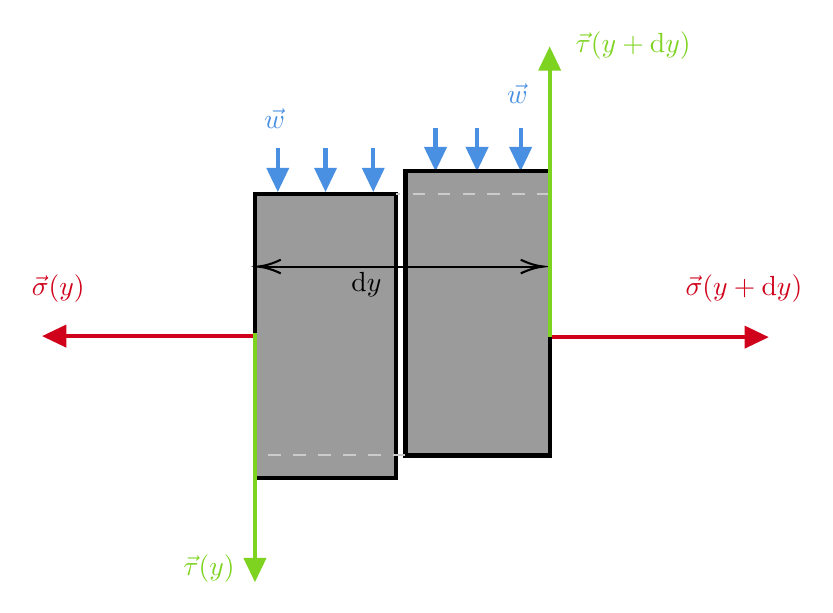
\begin{tikzpicture}[x=0.75pt,y=0.75pt,yscale=-1,xscale=1]
		%uncomment if require: \path (0,1215); %set diagram left start at 0, and has height of 1215
		
		%Straight Lines [id:da3954525570777263] 
		\draw [color={rgb, 255:red, 208; green, 2; blue, 27 }  ,draw opacity=1 ][line width=1.5]    (250,168.5) -- (149.5,168.5) ;
		\draw [shift={(145.5,168.5)}, rotate = 360] [fill={rgb, 255:red, 208; green, 2; blue, 27 }  ,fill opacity=1 ][line width=0.08]  [draw opacity=0] (11.61,-5.58) -- (0,0) -- (11.61,5.58) -- cycle    ;
		%Straight Lines [id:da1467450967819428] 
		\draw [color={rgb, 255:red, 208; green, 2; blue, 27 }  ,draw opacity=1 ][line width=1.5]    (390,169) -- (491.5,169) ;
		\draw [shift={(495.5,169)}, rotate = 180] [fill={rgb, 255:red, 208; green, 2; blue, 27 }  ,fill opacity=1 ][line width=0.08]  [draw opacity=0] (11.61,-5.58) -- (0,0) -- (11.61,5.58) -- cycle    ;
		%Straight Lines [id:da2605415787168175] 
		\draw [color={rgb, 255:red, 74; green, 144; blue, 226 }  ,draw opacity=1 ][line width=1.5]    (259,78) -- (259,95) ;
		\draw [shift={(259,99)}, rotate = 270] [fill={rgb, 255:red, 74; green, 144; blue, 226 }  ,fill opacity=1 ][line width=0.08]  [draw opacity=0] (11.61,-5.58) -- (0,0) -- (11.61,5.58) -- cycle    ;
		%Straight Lines [id:da3250672832580852] 
		\draw [color={rgb, 255:red, 74; green, 144; blue, 226 }  ,draw opacity=1 ][line width=1.5]    (282,78) -- (282,95) ;
		\draw [shift={(282,99)}, rotate = 270] [fill={rgb, 255:red, 74; green, 144; blue, 226 }  ,fill opacity=1 ][line width=0.08]  [draw opacity=0] (11.61,-5.58) -- (0,0) -- (11.61,5.58) -- cycle    ;
		%Straight Lines [id:da8483440483141562] 
		\draw [color={rgb, 255:red, 74; green, 144; blue, 226 }  ,draw opacity=1 ][line width=1.5]    (305,78) -- (305,95) ;
		\draw [shift={(305,99)}, rotate = 270] [fill={rgb, 255:red, 74; green, 144; blue, 226 }  ,fill opacity=1 ][line width=0.08]  [draw opacity=0] (11.61,-5.58) -- (0,0) -- (11.61,5.58) -- cycle    ;
		%Straight Lines [id:da8903474014081705] 
		\draw [color={rgb, 255:red, 74; green, 144; blue, 226 }  ,draw opacity=1 ][line width=1.5]    (335,68) -- (335,85) ;
		\draw [shift={(335,89)}, rotate = 270] [fill={rgb, 255:red, 74; green, 144; blue, 226 }  ,fill opacity=1 ][line width=0.08]  [draw opacity=0] (11.61,-5.58) -- (0,0) -- (11.61,5.58) -- cycle    ;
		%Straight Lines [id:da7258572747379872] 
		\draw [color={rgb, 255:red, 74; green, 144; blue, 226 }  ,draw opacity=1 ][line width=1.5]    (355,68) -- (355,85) ;
		\draw [shift={(355,89)}, rotate = 270] [fill={rgb, 255:red, 74; green, 144; blue, 226 }  ,fill opacity=1 ][line width=0.08]  [draw opacity=0] (11.61,-5.58) -- (0,0) -- (11.61,5.58) -- cycle    ;
		%Straight Lines [id:da1647458992707036] 
		\draw [color={rgb, 255:red, 74; green, 144; blue, 226 }  ,draw opacity=1 ][line width=1.5]    (376,68) -- (376,85) ;
		\draw [shift={(376,89)}, rotate = 270] [fill={rgb, 255:red, 74; green, 144; blue, 226 }  ,fill opacity=1 ][line width=0.08]  [draw opacity=0] (11.61,-5.58) -- (0,0) -- (11.61,5.58) -- cycle    ;
		%Shape: Rectangle [id:dp5668946685046703] 
		\draw  [fill={rgb, 255:red, 155; green, 155; blue, 155 }  ,fill opacity=1 ][line width=1.5]  (248,100) -- (316,100) -- (316,237) -- (248,237) -- cycle ;
		%Shape: Rectangle [id:dp8207058010622037] 
		\draw  [fill={rgb, 255:red, 155; green, 155; blue, 155 }  ,fill opacity=1 ][line width=1.5]  (320.5,89) -- (390,89) -- (390,226) -- (320.5,226) -- cycle ;
		%Straight Lines [id:da39162461512015834] 
		\draw [color={rgb, 255:red, 204; green, 204; blue, 204 }  ,draw opacity=1 ] [dash pattern={on 4.5pt off 4.5pt}]  (390,100) -- (316,100) ;
		%Straight Lines [id:da5090346039052429] 
		\draw [color={rgb, 255:red, 204; green, 204; blue, 204 }  ,draw opacity=1 ] [dash pattern={on 4.5pt off 4.5pt}]  (320.5,226) -- (249,226) ;
		%Straight Lines [id:da04551856417568456] 
		\draw    (251.5,135) -- (385,135) ;
		\draw [shift={(387,135)}, rotate = 180] [color={rgb, 255:red, 0; green, 0; blue, 0 }  ][line width=0.75]    (10.93,-3.29) .. controls (6.95,-1.4) and (3.31,-0.3) .. (0,0) .. controls (3.31,0.3) and (6.95,1.4) .. (10.93,3.29)   ;
		\draw [shift={(249.5,135)}, rotate = 0] [color={rgb, 255:red, 0; green, 0; blue, 0 }  ][line width=0.75]    (10.93,-3.29) .. controls (6.95,-1.4) and (3.31,-0.3) .. (0,0) .. controls (3.31,0.3) and (6.95,1.4) .. (10.93,3.29)   ;
		%Straight Lines [id:da2129953645023812] 
		\draw [color={rgb, 255:red, 126; green, 211; blue, 33 }  ,draw opacity=1 ][line width=1.5]    (248,167) -- (248,283) ;
		\draw [shift={(248,287)}, rotate = 270] [fill={rgb, 255:red, 126; green, 211; blue, 33 }  ,fill opacity=1 ][line width=0.08]  [draw opacity=0] (11.61,-5.58) -- (0,0) -- (11.61,5.58) -- cycle    ;
		%Straight Lines [id:da7485135934987044] 
		\draw [color={rgb, 255:red, 126; green, 211; blue, 33 }  ,draw opacity=1 ][line width=1.5]    (390,169) -- (390,33) ;
		\draw [shift={(390,29)}, rotate = 90] [fill={rgb, 255:red, 126; green, 211; blue, 33 }  ,fill opacity=1 ][line width=0.08]  [draw opacity=0] (11.61,-5.58) -- (0,0) -- (11.61,5.58) -- cycle    ;
		
		% Text Node
		\draw (139,137.4) node [anchor=north west][inner sep=0.75pt]  [color={rgb, 255:red, 208; green, 2; blue, 27 }  ,opacity=1 ]  {$\vec{\sigma }( y)$};
		% Text Node
		\draw (454,137.4) node [anchor=north west][inner sep=0.75pt]  [color={rgb, 255:red, 208; green, 2; blue, 27 }  ,opacity=1 ]  {$\vec{\sigma }( y+\mathrm{d} y)$};
		% Text Node
		\draw (293,136.4) node [anchor=north west][inner sep=0.75pt]    {$\mathrm{d} y$};
		% Text Node
		\draw (251,57.4) node [anchor=north west][inner sep=0.75pt]  [color={rgb, 255:red, 74; green, 144; blue, 226 }  ,opacity=1 ]  {$\vec{w}$};
		% Text Node
		\draw (368,45.4) node [anchor=north west][inner sep=0.75pt]  [color={rgb, 255:red, 74; green, 144; blue, 226 }  ,opacity=1 ]  {$\vec{w}$};
		% Text Node
		\draw (212,272.4) node [anchor=north west][inner sep=0.75pt]  [color={rgb, 255:red, 126; green, 211; blue, 33 }  ,opacity=1 ]  {$\vec{\tau }( y)$};
		% Text Node
		\draw (401,20.4) node [anchor=north west][inner sep=0.75pt]  [color={rgb, 255:red, 126; green, 211; blue, 33 }  ,opacity=1 ]  {$\vec{\tau }( y+\mathrm{d} y)$};
		\end{tikzpicture}
	\end{figure}
	That is to say algebraically (the variational can be negative or positive whatever!):
	
	And finally for the bending moments the sum is also necessarily zero at equilibrium. However, in contrast to the two preceding algebraic sums where we could only use the differential, we have to choose a reference point $R$ for the bending moments since, for recall... the moment of force is by definition the product of a force by a distance. We will therefore naturally choose the center of gravity:
	\begin{figure}[H]
		\centering
		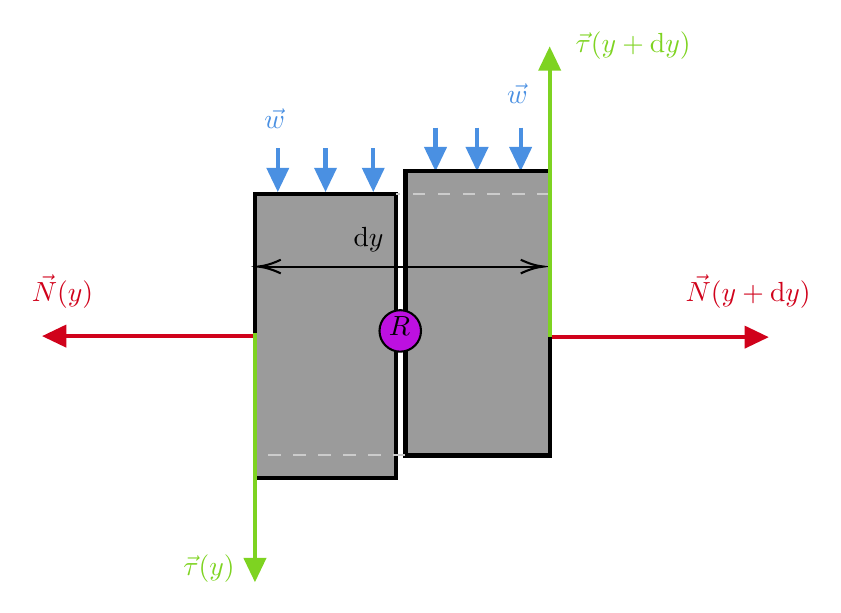
\begin{tikzpicture}[x=0.75pt,y=0.75pt,yscale=-1,xscale=1]
		%uncomment if require: \path (0,1215); %set diagram left start at 0, and has height of 1215
		
		%Straight Lines [id:da3954525570777263] 
		\draw [color={rgb, 255:red, 208; green, 2; blue, 27 }  ,draw opacity=1 ][line width=1.5]    (250,168.5) -- (149.5,168.5) ;
		\draw [shift={(145.5,168.5)}, rotate = 360] [fill={rgb, 255:red, 208; green, 2; blue, 27 }  ,fill opacity=1 ][line width=0.08]  [draw opacity=0] (11.61,-5.58) -- (0,0) -- (11.61,5.58) -- cycle    ;
		%Straight Lines [id:da1467450967819428] 
		\draw [color={rgb, 255:red, 208; green, 2; blue, 27 }  ,draw opacity=1 ][line width=1.5]    (390,169) -- (491.5,169) ;
		\draw [shift={(495.5,169)}, rotate = 180] [fill={rgb, 255:red, 208; green, 2; blue, 27 }  ,fill opacity=1 ][line width=0.08]  [draw opacity=0] (11.61,-5.58) -- (0,0) -- (11.61,5.58) -- cycle    ;
		%Straight Lines [id:da2605415787168175] 
		\draw [color={rgb, 255:red, 74; green, 144; blue, 226 }  ,draw opacity=1 ][line width=1.5]    (259,78) -- (259,95) ;
		\draw [shift={(259,99)}, rotate = 270] [fill={rgb, 255:red, 74; green, 144; blue, 226 }  ,fill opacity=1 ][line width=0.08]  [draw opacity=0] (11.61,-5.58) -- (0,0) -- (11.61,5.58) -- cycle    ;
		%Straight Lines [id:da3250672832580852] 
		\draw [color={rgb, 255:red, 74; green, 144; blue, 226 }  ,draw opacity=1 ][line width=1.5]    (282,78) -- (282,95) ;
		\draw [shift={(282,99)}, rotate = 270] [fill={rgb, 255:red, 74; green, 144; blue, 226 }  ,fill opacity=1 ][line width=0.08]  [draw opacity=0] (11.61,-5.58) -- (0,0) -- (11.61,5.58) -- cycle    ;
		%Straight Lines [id:da8483440483141562] 
		\draw [color={rgb, 255:red, 74; green, 144; blue, 226 }  ,draw opacity=1 ][line width=1.5]    (305,78) -- (305,95) ;
		\draw [shift={(305,99)}, rotate = 270] [fill={rgb, 255:red, 74; green, 144; blue, 226 }  ,fill opacity=1 ][line width=0.08]  [draw opacity=0] (11.61,-5.58) -- (0,0) -- (11.61,5.58) -- cycle    ;
		%Straight Lines [id:da8903474014081705] 
		\draw [color={rgb, 255:red, 74; green, 144; blue, 226 }  ,draw opacity=1 ][line width=1.5]    (335,68) -- (335,85) ;
		\draw [shift={(335,89)}, rotate = 270] [fill={rgb, 255:red, 74; green, 144; blue, 226 }  ,fill opacity=1 ][line width=0.08]  [draw opacity=0] (11.61,-5.58) -- (0,0) -- (11.61,5.58) -- cycle    ;
		%Straight Lines [id:da7258572747379872] 
		\draw [color={rgb, 255:red, 74; green, 144; blue, 226 }  ,draw opacity=1 ][line width=1.5]    (355,68) -- (355,85) ;
		\draw [shift={(355,89)}, rotate = 270] [fill={rgb, 255:red, 74; green, 144; blue, 226 }  ,fill opacity=1 ][line width=0.08]  [draw opacity=0] (11.61,-5.58) -- (0,0) -- (11.61,5.58) -- cycle    ;
		%Straight Lines [id:da1647458992707036] 
		\draw [color={rgb, 255:red, 74; green, 144; blue, 226 }  ,draw opacity=1 ][line width=1.5]    (376,68) -- (376,85) ;
		\draw [shift={(376,89)}, rotate = 270] [fill={rgb, 255:red, 74; green, 144; blue, 226 }  ,fill opacity=1 ][line width=0.08]  [draw opacity=0] (11.61,-5.58) -- (0,0) -- (11.61,5.58) -- cycle    ;
		%Shape: Rectangle [id:dp5668946685046703] 
		\draw  [fill={rgb, 255:red, 155; green, 155; blue, 155 }  ,fill opacity=1 ][line width=1.5]  (248,100) -- (316,100) -- (316,237) -- (248,237) -- cycle ;
		%Shape: Rectangle [id:dp8207058010622037] 
		\draw  [fill={rgb, 255:red, 155; green, 155; blue, 155 }  ,fill opacity=1 ][line width=1.5]  (320.5,89) -- (390,89) -- (390,226) -- (320.5,226) -- cycle ;
		%Straight Lines [id:da39162461512015834] 
		\draw [color={rgb, 255:red, 204; green, 204; blue, 204 }  ,draw opacity=1 ] [dash pattern={on 4.5pt off 4.5pt}]  (390,100) -- (316,100) ;
		%Straight Lines [id:da5090346039052429] 
		\draw [color={rgb, 255:red, 204; green, 204; blue, 204 }  ,draw opacity=1 ] [dash pattern={on 4.5pt off 4.5pt}]  (320.5,226) -- (249,226) ;
		%Straight Lines [id:da04551856417568456] 
		\draw    (251.5,135) -- (385,135) ;
		\draw [shift={(387,135)}, rotate = 180] [color={rgb, 255:red, 0; green, 0; blue, 0 }  ][line width=0.75]    (10.93,-3.29) .. controls (6.95,-1.4) and (3.31,-0.3) .. (0,0) .. controls (3.31,0.3) and (6.95,1.4) .. (10.93,3.29)   ;
		\draw [shift={(249.5,135)}, rotate = 0] [color={rgb, 255:red, 0; green, 0; blue, 0 }  ][line width=0.75]    (10.93,-3.29) .. controls (6.95,-1.4) and (3.31,-0.3) .. (0,0) .. controls (3.31,0.3) and (6.95,1.4) .. (10.93,3.29)   ;
		%Straight Lines [id:da2129953645023812] 
		\draw [color={rgb, 255:red, 126; green, 211; blue, 33 }  ,draw opacity=1 ][line width=1.5]    (248,167) -- (248,283) ;
		\draw [shift={(248,287)}, rotate = 270] [fill={rgb, 255:red, 126; green, 211; blue, 33 }  ,fill opacity=1 ][line width=0.08]  [draw opacity=0] (11.61,-5.58) -- (0,0) -- (11.61,5.58) -- cycle    ;
		%Straight Lines [id:da7485135934987044] 
		\draw [color={rgb, 255:red, 126; green, 211; blue, 33 }  ,draw opacity=1 ][line width=1.5]    (390,169) -- (390,33) ;
		\draw [shift={(390,29)}, rotate = 90] [fill={rgb, 255:red, 126; green, 211; blue, 33 }  ,fill opacity=1 ][line width=0.08]  [draw opacity=0] (11.61,-5.58) -- (0,0) -- (11.61,5.58) -- cycle    ;
		%Shape: Circle [id:dp44881326045563563] 
		\draw  [fill={rgb, 255:red, 189; green, 16; blue, 224 }  ,fill opacity=1 ] (308,166) .. controls (308,160.48) and (312.48,156) .. (318,156) .. controls (323.52,156) and (328,160.48) .. (328,166) .. controls (328,171.52) and (323.52,176) .. (318,176) .. controls (312.48,176) and (308,171.52) .. (308,166) -- cycle ;
		
		% Text Node
		\draw (139,137.4) node [anchor=north west][inner sep=0.75pt]  [color={rgb, 255:red, 208; green, 2; blue, 27 }  ,opacity=1 ]  {$\vec{N}( y)$};
		% Text Node
		\draw (454,137.4) node [anchor=north west][inner sep=0.75pt]  [color={rgb, 255:red, 208; green, 2; blue, 27 }  ,opacity=1 ]  {$\vec{N}( y+\mathrm{d} y)$};
		% Text Node
		\draw (294,114.4) node [anchor=north west][inner sep=0.75pt]    {$\mathrm{d} y$};
		% Text Node
		\draw (251,57.4) node [anchor=north west][inner sep=0.75pt]  [color={rgb, 255:red, 74; green, 144; blue, 226 }  ,opacity=1 ]  {$\vec{w}$};
		% Text Node
		\draw (368,45.4) node [anchor=north west][inner sep=0.75pt]  [color={rgb, 255:red, 74; green, 144; blue, 226 }  ,opacity=1 ]  {$\vec{w}$};
		% Text Node
		\draw (212,272.4) node [anchor=north west][inner sep=0.75pt]  [color={rgb, 255:red, 126; green, 211; blue, 33 }  ,opacity=1 ]  {$\vec{\tau }( y)$};
		% Text Node
		\draw (401,20.4) node [anchor=north west][inner sep=0.75pt]  [color={rgb, 255:red, 126; green, 211; blue, 33 }  ,opacity=1 ]  {$\vec{\tau }( y+\mathrm{d} y)$};
		% Text Node
		\draw (311,157.4) node [anchor=north west][inner sep=0.75pt]    {$R$};
		\end{tikzpicture}
	\end{figure}
	The uniform linear load $\vec{w}$ on the length $\mathrm{d}y$ generates a force at mid distance of:
	
	but as it is confounded with the choices of our reference point, then its moment of strength is zero!

	We then have algebraically:
	
	And if we neglect the differentials of order two it remains only:
	
	Finally, we have:
	
	To determine the bending moment from the linear load (which is of primary interest to the practitioner), we derive the third relation twice and make a substitution:
	
	Hence:
	
	The problem with this last relation is the knowledge of the moments. We should get rid of this term absolutely. What we know easily is the deformation function and we have proved earlier above that:
	
	It then comes immediately by substituting the preceding relation in the prior previous one:
	
	where the product $EI$ is known as the "\NewTerm{flexural rigidity}".
	
	This is the most important elementary relation of the theory of beams, that covers the case for small deflections of a beam that is subjected to lateral loads only, because it allows by knowing the linear load to determine the function of deformation or conversely! It is so important to know that it is named the "\NewTerm{static beam equation}\index{static beam equation}" or in honour to those who have determined it: "\NewTerm{Euler-Bernoulli equation}\index{Euler-Bernoulli equation}".  It seemed it was first enunciated circa 11750 (holocene calendar), but was not applied on a large scale until the development of the Eiffel Tower and the Ferris wheel in the late 119th century (holocene calendar).

	Since it is a differential equation of order $4$ that will generate four constants at each integration, we will then need $4$ initial conditions to solve it completely.
	\begin{tcolorbox}[title=Remark,arc=10pt,breakable,drop lifted shadow,
  skin=enhanced,
  skin first is subskin of={enhancedfirst}{arc=10pt,no shadow},
  skin middle is subskin of={enhancedmiddle}{arc=10pt,no shadow},
  skin last is subskin of={enhancedlast}{drop lifted shadow}]
	The Euler-Bernoulli equation by its assumptions is only a special case of a more general theory named the "\NewTerm{Timoshenko beam theory}\index{Timoshenko beam theory}" published in 11921 (holocene calendar).
	\end{tcolorbox}
	
	\begin{tcolorbox}[colframe=black,colback=white,sharp corners,breakable]
	\textbf{{\Large \ding{45}}Example:}\\\\
	We would like to calculate the deformation of a beam fixed on both sides and loaded uniformly knowing its length $L$, its modulus of elasticity $E$, its moment of inertia $I$. \\

	We start from (we change the notations only to show that according to some textbooks the axes can be denoted differently):
	
	With the initial conditions:
	
	And integrating by repetition, we have:
	
	From the two initial conditions:
	
	It follows that:
	
	With the other two remaining conditions, we obtain the following system which must allow us to determine the two remaining constants:
	
	Then it is simply a matter of solving a simple linear system (\SeeChapter{see section Linear Algebra page \pageref{linear systems}}):
	
	Subtracting both relation in the simple adequate way we get immediately:
	
	Therefore for an ideal beam embedded on both sides subjected to a uniform load and described by:
	
	To determine the arrow, we must therefore look for the point $x$ where this relation has an optimum. We then have:
	
	It follows that the arrow has a maximum at $x = L / 2$. Injecting this into $y (x)$ we get the famous relation often given in the literature but rarely proved:
	
	It follows that the arrow of a beam is proportional to the fourth power of the length of the beam! Such high dependence imposes significant limitations on Civil Engineering structures based on beams.
	\end{tcolorbox}
	\begin{tcolorbox}[title=Remark,arc=10pt,breakable,drop lifted shadow,
  skin=enhanced,
  skin first is subskin of={enhancedfirst}{arc=10pt,no shadow},
  skin middle is subskin of={enhancedmiddle}{arc=10pt,no shadow},
  skin last is subskin of={enhancedlast}{drop lifted shadow}]
	The constant linear load, either over the total length of the beam or in successive sections, is a frequent observed type of stress in horizontal axis of pieces. It may come from the weight of the pieces with a constant section or from a load caused by an external force (eg gravity).
	\end{tcolorbox}
	
	\pagebreak
	\paragraph{Potential elastic energy}\mbox{}\\\\
	After a quick overview of the various elastic deformations of the parts stressed by the fundamental forces, we will establish here the general expression of the elastic energy accumulated in a beam of any shape stressed by external forces.

	Let us recall for this study that we can write Hook's law (\SeeChapter{see section Continuum Mechanics page \pageref{hooke law}}) in the following form:
	
	and the elastic potential energy of a spring proved in the section of Classical Mechanics (see page \pageref{potential energy harmonic oscillator}) is given by:
	
	Or in relative displacement:
	
	In the traction domain (or compression) of the beams, it is customary to consider the beam as a spring (...) and then to use the stiffness constant of Hook's law ... hoping that this is conforming to experimental observations...:
	
	Where, according to usage, we denote the longitudinal displacement $L$ instead of $x$. By injecting Hook's law (yes ... it turns a little bit a loop... but that's engineering...):
	
	It is then sufficient to divide by the length of the bar to have the elastic linear energy denoted:
	
	The energy density, noted conventionally denoted as in thermodynamics by a minuscule letter, is then:
	
	
	\pagebreak
	\subsubsection{Torsion}\label{torsion}
	Let us recall first to the reader a study we made in the section on Classical Mechanics on the torsional pendulum where some elements had deliberately been muted.... Let's study this in more detail as it is very useful for transmission shafts or springs in everyday life.

	Let us consider for this a cylindrical wire fixed at its base and subjected to a torsion moment $\vec{M}$. Under the effect of this torsion moment, the upper face of the wire is offset by an angle $\theta$ with respect to the lower face, the material undergoing a torsion stress (or shearing $\tau$):
	\begin{figure}[H]
		\centering
		\begin{tikzpicture}[x=0.75pt,y=0.75pt,yscale=-1,xscale=1]
		%uncomment if require: \path (0,1077); %set diagram left start at 0, and has height of 1077
		
		% Pattern Info
		 
		\tikzset{
		pattern size/.store in=\mcSize, 
		pattern size = 5pt,
		pattern thickness/.store in=\mcThickness, 
		pattern thickness = 0.3pt,
		pattern radius/.store in=\mcRadius, 
		pattern radius = 1pt}
		\makeatletter
		\pgfutil@ifundefined{pgf@pattern@name@_dukr3qow2}{
		\pgfdeclarepatternformonly[\mcThickness,\mcSize]{_dukr3qow2}
		{\pgfqpoint{0pt}{0pt}}
		{\pgfpoint{\mcSize+\mcThickness}{\mcSize+\mcThickness}}
		{\pgfpoint{\mcSize}{\mcSize}}
		{
		\pgfsetcolor{\tikz@pattern@color}
		\pgfsetlinewidth{\mcThickness}
		\pgfpathmoveto{\pgfqpoint{0pt}{0pt}}
		\pgfpathlineto{\pgfpoint{\mcSize+\mcThickness}{\mcSize+\mcThickness}}
		\pgfusepath{stroke}
		}}
		
		%Shape: Cube [id:dp22830729803430172] 
		\draw  [fill={rgb, 255:red, 224; green, 224; blue, 224 }  ,fill opacity=1 ] (103,369.24) -- (209.24,263) -- (562,263) -- (562,301.76) -- (455.76,408) -- (103,408) -- cycle ; \draw   (562,263) -- (455.76,369.24) -- (103,369.24) ; \draw   (455.76,369.24) -- (455.76,408) ;
		%Shape: Can [id:dp3422118573809392] 
		\draw  [line width=1.5]  (425,133.65) -- (425,319.35) .. controls (425,335.17) and (382.24,348) .. (329.5,348) .. controls (276.76,348) and (234,335.17) .. (234,319.35) -- (234,133.65) .. controls (234,117.83) and (276.76,105) .. (329.5,105) .. controls (382.24,105) and (425,117.83) .. (425,133.65) .. controls (425,149.47) and (382.24,162.3) .. (329.5,162.3) .. controls (276.76,162.3) and (234,149.47) .. (234,133.65) ;
		%Shape: Arc [id:dp06064822823432592] 
		\draw  [draw opacity=0][dash pattern={on 5.63pt off 4.5pt}][line width=1.5]  (234.4,313.48) .. controls (238.84,296.43) and (279.8,283.08) .. (329.67,283.08) .. controls (382.5,283.08) and (425.33,298.07) .. (425.33,316.55) .. controls (425.33,317.5) and (425.22,318.43) .. (425,319.35) -- (329.67,316.55) -- cycle ; \draw  [color={rgb, 255:red, 155; green, 155; blue, 155 }  ,draw opacity=1 ][dash pattern={on 5.63pt off 4.5pt}][line width=1.5]  (234.4,313.48) .. controls (238.84,296.43) and (279.8,283.08) .. (329.67,283.08) .. controls (382.5,283.08) and (425.33,298.07) .. (425.33,316.55) .. controls (425.33,317.5) and (425.22,318.43) .. (425,319.35) ;  
		%Straight Lines [id:da7199367607398894] 
		\draw    (188,133.65) -- (234,133.65) ;
		%Straight Lines [id:da11146887263152871] 
		\draw    (198,138) -- (198,316) ;
		\draw [shift={(198,318)}, rotate = 270] [color={rgb, 255:red, 0; green, 0; blue, 0 }  ][line width=0.75]    (10.93,-3.29) .. controls (6.95,-1.4) and (3.31,-0.3) .. (0,0) .. controls (3.31,0.3) and (6.95,1.4) .. (10.93,3.29)   ;
		\draw [shift={(198,136)}, rotate = 90] [color={rgb, 255:red, 0; green, 0; blue, 0 }  ][line width=0.75]    (10.93,-3.29) .. controls (6.95,-1.4) and (3.31,-0.3) .. (0,0) .. controls (3.31,0.3) and (6.95,1.4) .. (10.93,3.29)   ;
		%Straight Lines [id:da572560008257379] 
		\draw    (234,319.35) -- (234,394) ;
		%Straight Lines [id:da5963171649224985] 
		\draw    (425,319.35) -- (425,394) ;
		%Straight Lines [id:da8505914619747288] 
		\draw    (188,319.35) -- (234,319.35) ;
		%Straight Lines [id:da14778473612010212] 
		\draw    (236,384) -- (423,384) ;
		\draw [shift={(425,384)}, rotate = 180] [color={rgb, 255:red, 0; green, 0; blue, 0 }  ][line width=0.75]    (10.93,-3.29) .. controls (6.95,-1.4) and (3.31,-0.3) .. (0,0) .. controls (3.31,0.3) and (6.95,1.4) .. (10.93,3.29)   ;
		\draw [shift={(234,384)}, rotate = 0] [color={rgb, 255:red, 0; green, 0; blue, 0 }  ][line width=0.75]    (10.93,-3.29) .. controls (6.95,-1.4) and (3.31,-0.3) .. (0,0) .. controls (3.31,0.3) and (6.95,1.4) .. (10.93,3.29)   ;
		%Shape: Ellipse [id:dp48827816894156917] 
		\draw  [pattern=_dukr3qow2,pattern size=6pt,pattern thickness=0.75pt,pattern radius=0pt, pattern color={rgb, 255:red, 0; green, 0; blue, 0}] (263.17,133.35) .. controls (263.17,122.69) and (291.97,114.05) .. (327.5,114.05) .. controls (363.03,114.05) and (391.83,122.69) .. (391.83,133.35) .. controls (391.83,144.01) and (363.03,152.65) .. (327.5,152.65) .. controls (291.97,152.65) and (263.17,144.01) .. (263.17,133.35) -- cycle ;
		%Shape: Ellipse [id:dp5038475086116145] 
		\draw  [fill={rgb, 255:red, 255; green, 255; blue, 255 }  ,fill opacity=1 ] (279.12,133.35) .. controls (279.12,126.37) and (300.78,120.71) .. (327.5,120.71) .. controls (354.22,120.71) and (375.88,126.37) .. (375.88,133.35) .. controls (375.88,140.33) and (354.22,145.99) .. (327.5,145.99) .. controls (300.78,145.99) and (279.12,140.33) .. (279.12,133.35) -- cycle ;
		%Straight Lines [id:da5002967069288613] 
		\draw    (327,76) -- (327,362) ;
		%Straight Lines [id:da9406244836279829] 
		\draw    (263.17,58.7) -- (263.17,133.35) ;
		%Straight Lines [id:da4833248892673532] 
		\draw    (391.83,58.7) -- (391.83,133.35) ;
		%Straight Lines [id:da9437309774848577] 
		\draw    (266,66) -- (389,66) ;
		\draw [shift={(391,66)}, rotate = 180] [color={rgb, 255:red, 0; green, 0; blue, 0 }  ][line width=0.75]    (10.93,-3.29) .. controls (6.95,-1.4) and (3.31,-0.3) .. (0,0) .. controls (3.31,0.3) and (6.95,1.4) .. (10.93,3.29)   ;
		\draw [shift={(264,66)}, rotate = 0] [color={rgb, 255:red, 0; green, 0; blue, 0 }  ][line width=0.75]    (10.93,-3.29) .. controls (6.95,-1.4) and (3.31,-0.3) .. (0,0) .. controls (3.31,0.3) and (6.95,1.4) .. (10.93,3.29)   ;
		%Straight Lines [id:da8566223202934511] 
		\draw [color={rgb, 255:red, 144; green, 19; blue, 254 }  ,draw opacity=1 ][line width=1.5]    (327,76) -- (327,28) ;
		\draw [shift={(327,24)}, rotate = 90] [fill={rgb, 255:red, 144; green, 19; blue, 254 }  ,fill opacity=1 ][line width=0.08]  [draw opacity=0] (11.61,-5.58) -- (0,0) -- (11.61,5.58) -- cycle    ;
		%Straight Lines [id:da38925260871612455] 
		\draw    (382,137) -- (442,190) -- (487,190) ;
		%Straight Lines [id:da9712991338399048] 
		\draw [color={rgb, 255:red, 208; green, 2; blue, 27 }  ,draw opacity=1 ][line width=1.5]    (408,151) -- (452.58,124.07) ;
		\draw [shift={(456,122)}, rotate = 148.86] [fill={rgb, 255:red, 208; green, 2; blue, 27 }  ,fill opacity=1 ][line width=0.08]  [draw opacity=0] (11.61,-5.58) -- (0,0) -- (11.61,5.58) -- cycle    ;
		%Straight Lines [id:da6229188762042766] 
		\draw    (279.5,112.3) -- (298,132) ;
		%Straight Lines [id:da14452788176346854] 
		\draw    (279.5,112.3) -- (287.38,120.69) ;
		\draw [shift={(288.75,122.15)}, rotate = 226.8] [color={rgb, 255:red, 0; green, 0; blue, 0 }  ][line width=0.75]    (10.93,-3.29) .. controls (6.95,-1.4) and (3.31,-0.3) .. (0,0) .. controls (3.31,0.3) and (6.95,1.4) .. (10.93,3.29)   ;
		%Straight Lines [id:da9786620764080436] 
		\draw    (298,132) -- (290.12,123.61) ;
		\draw [shift={(288.75,122.15)}, rotate = 46.8] [color={rgb, 255:red, 0; green, 0; blue, 0 }  ][line width=0.75]    (10.93,-3.29) .. controls (6.95,-1.4) and (3.31,-0.3) .. (0,0) .. controls (3.31,0.3) and (6.95,1.4) .. (10.93,3.29)   ;
		%Straight Lines [id:da22787681226696788] 
		\draw [color={rgb, 255:red, 155; green, 155; blue, 155 }  ,draw opacity=1 ] [dash pattern={on 4.5pt off 4.5pt}]  (263.17,133.35) -- (263.17,314) ;
		%Straight Lines [id:da8182616364686681] 
		\draw [color={rgb, 255:red, 155; green, 155; blue, 155 }  ,draw opacity=1 ] [dash pattern={on 4.5pt off 4.5pt}]  (391.83,133.35) -- (391.83,186) -- (391.83,314) ;
		%Shape: Ellipse [id:dp302978027733805] 
		\draw  [color={rgb, 255:red, 155; green, 155; blue, 155 }  ,draw opacity=1 ][dash pattern={on 4.5pt off 4.5pt}] (263.17,314) .. controls (263.17,303.34) and (291.97,294.7) .. (327.5,294.7) .. controls (363.03,294.7) and (391.83,303.34) .. (391.83,314) .. controls (391.83,324.66) and (363.03,333.3) .. (327.5,333.3) .. controls (291.97,333.3) and (263.17,324.66) .. (263.17,314) -- cycle ;
		%Straight Lines [id:da37043436857768564] 
		\draw [line width=1.5]    (327.5,133.35) -- (327.5,145.99) ;
		%Curve Lines [id:da5353647791758782] 
		\draw [line width=1.5]    (327,348.2) .. controls (326.5,275.2) and (342,180.8) .. (357,161.8) ;
		%Shape: Arc [id:dp5584806016115795] 
		\draw  [draw opacity=0] (325.97,192.33) .. controls (326.17,192.33) and (326.36,192.32) .. (326.56,192.32) .. controls (333.43,192.32) and (339.5,195.69) .. (343.21,200.86) -- (326.56,212.66) -- cycle ; \draw   (325.97,192.33) .. controls (326.17,192.33) and (326.36,192.32) .. (326.56,192.32) .. controls (333.43,192.32) and (339.5,195.69) .. (343.21,200.86) ;  
		%Shape: Arc [id:dp9716343261070328] 
		\draw  [draw opacity=0][line width=2.25]  (347.9,151.52) .. controls (342.14,152.27) and (336.04,152.67) .. (329.73,152.67) .. controls (328.98,152.67) and (328.24,152.66) .. (327.5,152.65) -- (329.73,124.35) -- cycle ; \draw  [color={rgb, 255:red, 80; green, 227; blue, 194 }  ,draw opacity=1 ][line width=2.25]  (347.9,151.52) .. controls (342.14,152.27) and (336.04,152.67) .. (329.73,152.67) .. controls (328.98,152.67) and (328.24,152.66) .. (327.5,152.65) ;  
		%Straight Lines [id:da5753410305643758] 
		\draw    (334,153) -- (309,196) -- (282,196) ;
		%Straight Lines [id:da8541570058683943] 
		\draw [line width=1.5]    (327.5,133.35) -- (357,161.8) ;
		
		% Text Node
		\draw (174,219.4) node [anchor=north west][inner sep=0.75pt]    {$L$};
		% Text Node
		\draw (315,387.4) node [anchor=north west][inner sep=0.75pt]    {$2R$};
		% Text Node
		\draw (350,45.4) node [anchor=north west][inner sep=0.75pt]    {$2r$};
		% Text Node
		\draw (298,13.4) node [anchor=north west][inner sep=0.75pt]  [color={rgb, 255:red, 144; green, 19; blue, 254 }  ,opacity=1 ]  {$\vec{M}$};
		% Text Node
		\draw (452,168.4) node [anchor=north west][inner sep=0.75pt]    {$\mathrm{d} S$};
		% Text Node
		\draw (461,103.4) node [anchor=north west][inner sep=0.75pt]  [color={rgb, 255:red, 208; green, 2; blue, 27 }  ,opacity=1 ]  {$\vec{F}$};
		% Text Node
		\draw (300,122.4) node [anchor=north west][inner sep=0.75pt]    {$\mathrm{d} r$};
		% Text Node
		\draw (327.97,195.73) node [anchor=north west][inner sep=0.75pt]    {$\gamma $};
		% Text Node
		\draw (335,126.4) node [anchor=north west][inner sep=0.75pt]    {$\theta $};
		% Text Node
		\draw (285,177.4) node [anchor=north west][inner sep=0.75pt]  [color={rgb, 255:red, 80; green, 227; blue, 194 }  ,opacity=1 ]  {$r\theta $};
		\end{tikzpicture}
		\vspace*{3mm}
		\caption{Wire under torsion}
	\end{figure}
	Let us imagine an extraction of the inside the wire an elementary tube of radius $r$, of thickness $\mathrm{d}r$, and let us observe the effect of the torsion on this tube unrolled (this will allow us an approximate approach of the concerned phenomenon):
	\begin{figure}[H]
		\centering
		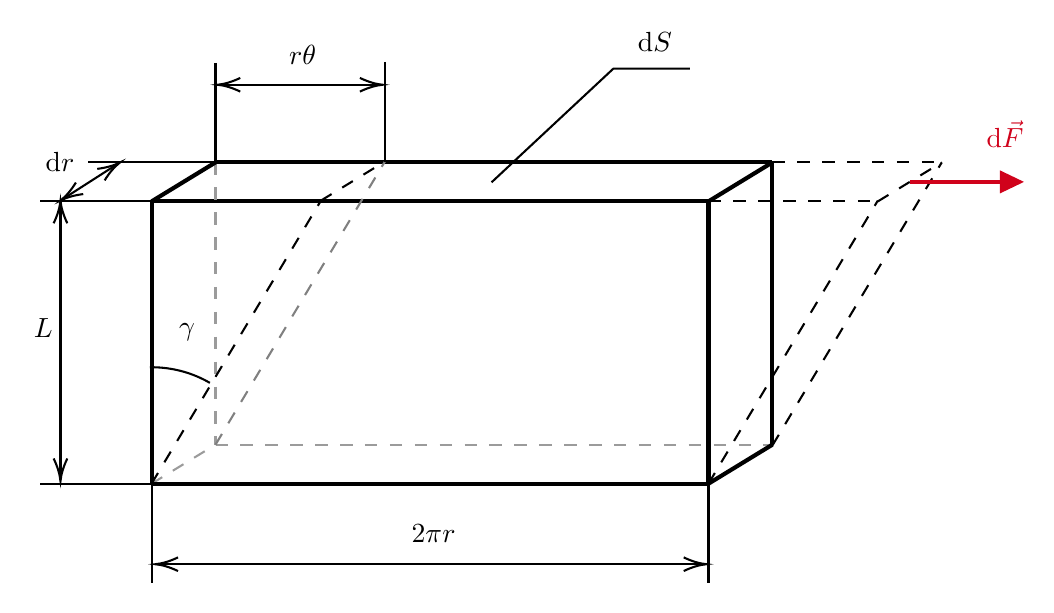
\begin{tikzpicture}[x=0.75pt,y=0.75pt,yscale=-1,xscale=1]
		%uncomment if require: \path (0,1215); %set diagram left start at 0, and has height of 1215
		
		%Straight Lines [id:da6171777705597701] 
		\draw [line width=1.5]    (137.2,178.2) -- (405.5,178.2) ;
		%Straight Lines [id:da7840143173948755] 
		\draw [line width=1.5]    (405.5,178.2) -- (436.3,159.4) ;
		%Straight Lines [id:da8945570606551561] 
		\draw [line width=1.5]    (405.5,314.2) -- (405.5,178.2) ;
		%Straight Lines [id:da412458199262532] 
		\draw [color={rgb, 255:red, 155; green, 155; blue, 155 }  ,draw opacity=1 ][line width=0.75]  [dash pattern={on 4.5pt off 4.5pt}]  (168,159.4) -- (168,295.4) ;
		%Straight Lines [id:da2009879025533503] 
		\draw [color={rgb, 255:red, 155; green, 155; blue, 155 }  ,draw opacity=1 ][line width=0.75]  [dash pattern={on 4.5pt off 4.5pt}]  (168,295.4) -- (436.3,295.4) ;
		%Straight Lines [id:da9689425487028014] 
		\draw [color={rgb, 255:red, 155; green, 155; blue, 155 }  ,draw opacity=1 ][line width=0.75]  [dash pattern={on 4.5pt off 4.5pt}]  (137.2,314.2) -- (168,295.4) ;
		%Straight Lines [id:da8426951698732894] 
		\draw [line width=1.5]    (168,159.4) -- (436.3,159.4) ;
		%Straight Lines [id:da2400787176569057] 
		\draw [line width=1.5]    (137.2,178.2) -- (168,159.4) ;
		%Straight Lines [id:da11417944407969216] 
		\draw [line width=1.5]    (137.2,178.2) -- (137.2,314.2) ;
		%Straight Lines [id:da16108677954411754] 
		\draw [line width=1.5]    (405.5,314.2) -- (137.2,314.2) ;
		%Straight Lines [id:da6320283374181404] 
		\draw [line width=1.5]    (436.3,295.4) -- (436.3,159.4) ;
		%Straight Lines [id:da7031945111056459] 
		\draw [line width=1.5]    (405.5,314.2) -- (436.3,295.4) ;
		%Straight Lines [id:da13808261571640013] 
		\draw  [dash pattern={on 4.5pt off 4.5pt}]  (137.2,314.2) -- (218.8,177.8) ;
		%Straight Lines [id:da9383418289289744] 
		\draw [line width=0.75]  [dash pattern={on 4.5pt off 4.5pt}]  (218.8,177.8) -- (249.6,159) ;
		%Straight Lines [id:da22717261095192853] 
		\draw [color={rgb, 255:red, 128; green, 128; blue, 128 }  ,draw opacity=1 ] [dash pattern={on 4.5pt off 4.5pt}]  (168,295.4) -- (249.6,159) ;
		%Straight Lines [id:da9621500114450501] 
		\draw [line width=0.75]  [dash pattern={on 4.5pt off 4.5pt}]  (405.5,178.2) -- (487.1,178.2) ;
		%Straight Lines [id:da8758212743024592] 
		\draw [line width=0.75]  [dash pattern={on 4.5pt off 4.5pt}]  (487.1,178.2) -- (517.9,159.4) ;
		%Straight Lines [id:da6531936009581789] 
		\draw  [dash pattern={on 4.5pt off 4.5pt}]  (405.5,314.2) -- (487.1,177.8) ;
		%Straight Lines [id:da12460829804390805] 
		\draw [line width=0.75]  [dash pattern={on 4.5pt off 4.5pt}]  (436.3,159.4) -- (517.9,159.4) ;
		%Straight Lines [id:da9893216964897968] 
		\draw  [dash pattern={on 4.5pt off 4.5pt}]  (436.3,295.8) -- (517.9,159.4) ;
		%Straight Lines [id:da18356621111460214] 
		\draw    (396.5,114.25) -- (359.66,114.25) -- (301,169) ;
		%Straight Lines [id:da6784373309152254] 
		\draw    (249.6,111) -- (249.6,159) ;
		%Straight Lines [id:da24610028248080562] 
		\draw    (168,111.4) -- (168,159.4) ;
		%Straight Lines [id:da4806393167657199] 
		\draw    (171,122) -- (246.5,122) ;
		\draw [shift={(248.5,122)}, rotate = 180] [color={rgb, 255:red, 0; green, 0; blue, 0 }  ][line width=0.75]    (10.93,-3.29) .. controls (6.95,-1.4) and (3.31,-0.3) .. (0,0) .. controls (3.31,0.3) and (6.95,1.4) .. (10.93,3.29)   ;
		\draw [shift={(169,122)}, rotate = 0] [color={rgb, 255:red, 0; green, 0; blue, 0 }  ][line width=0.75]    (10.93,-3.29) .. controls (6.95,-1.4) and (3.31,-0.3) .. (0,0) .. controls (3.31,0.3) and (6.95,1.4) .. (10.93,3.29)   ;
		%Shape: Arc [id:dp8164559881695768] 
		\draw  [draw opacity=0] (136.33,258.11) .. controls (136.62,258.1) and (136.91,258.1) .. (137.2,258.1) .. controls (147.43,258.1) and (157.03,260.84) .. (165.29,265.63) -- (137.2,314.2) -- cycle ; \draw   (136.33,258.11) .. controls (136.62,258.1) and (136.91,258.1) .. (137.2,258.1) .. controls (147.43,258.1) and (157.03,260.84) .. (165.29,265.63) ;  
		%Straight Lines [id:da7402540086151077] 
		\draw [color={rgb, 255:red, 208; green, 2; blue, 27 }  ,draw opacity=1 ][line width=1.5]    (502.5,168.8) -- (553.5,168.8) ;
		\draw [shift={(557.5,168.8)}, rotate = 180] [fill={rgb, 255:red, 208; green, 2; blue, 27 }  ,fill opacity=1 ][line width=0.08]  [draw opacity=0] (11.61,-5.58) -- (0,0) -- (11.61,5.58) -- cycle    ;
		%Straight Lines [id:da12851545284220767] 
		\draw    (137.2,314.2) -- (137.2,362.2) ;
		%Straight Lines [id:da8442649069822383] 
		\draw    (405.5,314.2) -- (405.5,362.2) ;
		%Straight Lines [id:da7488802015810156] 
		\draw    (141,353) -- (402.5,353) ;
		\draw [shift={(404.5,353)}, rotate = 180] [color={rgb, 255:red, 0; green, 0; blue, 0 }  ][line width=0.75]    (10.93,-3.29) .. controls (6.95,-1.4) and (3.31,-0.3) .. (0,0) .. controls (3.31,0.3) and (6.95,1.4) .. (10.93,3.29)   ;
		\draw [shift={(139,353)}, rotate = 0] [color={rgb, 255:red, 0; green, 0; blue, 0 }  ][line width=0.75]    (10.93,-3.29) .. controls (6.95,-1.4) and (3.31,-0.3) .. (0,0) .. controls (3.31,0.3) and (6.95,1.4) .. (10.93,3.29)   ;
		%Straight Lines [id:da569207027986911] 
		\draw    (168,159.4) -- (106.5,159.4) ;
		%Straight Lines [id:da5904740704782383] 
		\draw    (137.2,178.2) -- (83.5,178.2) ;
		%Straight Lines [id:da31175460523955834] 
		\draw    (94.98,176.72) -- (120.32,160.48) ;
		\draw [shift={(122,159.4)}, rotate = 147.34] [color={rgb, 255:red, 0; green, 0; blue, 0 }  ][line width=0.75]    (10.93,-3.29) .. controls (6.95,-1.4) and (3.31,-0.3) .. (0,0) .. controls (3.31,0.3) and (6.95,1.4) .. (10.93,3.29)   ;
		\draw [shift={(93.3,177.8)}, rotate = 327.34] [color={rgb, 255:red, 0; green, 0; blue, 0 }  ][line width=0.75]    (10.93,-3.29) .. controls (6.95,-1.4) and (3.31,-0.3) .. (0,0) .. controls (3.31,0.3) and (6.95,1.4) .. (10.93,3.29)   ;
		%Straight Lines [id:da4170810894528829] 
		\draw    (137.2,314.2) -- (83.5,314.2) ;
		%Straight Lines [id:da7453145515225819] 
		\draw    (93.3,311) -- (93.3,179.8) ;
		\draw [shift={(93.3,177.8)}, rotate = 90] [color={rgb, 255:red, 0; green, 0; blue, 0 }  ][line width=0.75]    (10.93,-3.29) .. controls (6.95,-1.4) and (3.31,-0.3) .. (0,0) .. controls (3.31,0.3) and (6.95,1.4) .. (10.93,3.29)   ;
		\draw [shift={(93.3,313)}, rotate = 270] [color={rgb, 255:red, 0; green, 0; blue, 0 }  ][line width=0.75]    (10.93,-3.29) .. controls (6.95,-1.4) and (3.31,-0.3) .. (0,0) .. controls (3.31,0.3) and (6.95,1.4) .. (10.93,3.29)   ;
		
		% Text Node
		\draw (370,95) node [anchor=north west][inner sep=0.75pt]    {$\mathrm{d}S$};
		% Text Node
		\draw (202,101.4) node [anchor=north west][inner sep=0.75pt]    {$r\theta $};
		% Text Node
		\draw (149,235.4) node [anchor=north west][inner sep=0.75pt]    {$\gamma $};
		% Text Node
		\draw (538,138) node [anchor=north west][inner sep=0.75pt]  [color={rgb, 255:red, 208; green, 2; blue, 27 }  ,opacity=1 ]  {$\mathrm{d}\vec{F}$};
		% Text Node
		\draw (261,332.4) node [anchor=north west][inner sep=0.75pt]    {$2\pi r$};
		% Text Node
		\draw (78,133.4) node [anchor=north west][inner sep=0.75pt]    {$ \begin{array}{l}
		\mathrm{d} r
		\end{array}$};
		% Text Node
		\draw (79,233.4) node [anchor=north west][inner sep=0.75pt]    {$L$};
		\end{tikzpicture}
		\vspace*{3mm}
		\caption[]{Extraction an unroll of an element of the wire} 
	\end{figure}
	Let us look for a relation between torsion moment $\vec{M}$ and torsion angle $\theta$ that would therefore also apply to a beam as below:
	\begin{figure}[H]
		\centering
		\includegraphics[scale=0.5]{img/engineering/rectangular_torsion_beam.jpg}
	\end{figure}
	For the unrolled tube, let us apply the shear relations as proved and introduced in the section of Continuum Mechanics (see page \pageref{shear modulus}):
	
	but the figure shows that (the deformations being weak) to the first order in Taylor series (\SeeChapter{see section Sequences and Series page \pageref{usual maclaurin developments}}):
	
	hence:
	
	The elementary moment due to this force is by definition of the moment of force (torque):
	
	Since $\vec{r}$ and $\vec{F}$ are perpendicular:
	
	The total moment (torque) is then equal to:
	
	therefore:
	
	We thus fall back on the relation of the torsional pendulum that we had found during our study of the torsional pendulum in the section of Classical Mechanics (see page \pageref{moment torsion pendulum}):
	
	 with the difference that this time the constant $k$, the "\NewTerm{torsion constant}\index{torsion constant}" is explicit!!!!

	The numerator of the constant $k$ is named in the domain of the strength of materials the "\NewTerm{torsional rigidity}\index{torsional rigidity}" or "\NewTerm{torsional stiffness}\index{torsional stiffness}" and the constant $k$ itself is often referred to as "\NewTerm{shaft rigidity}\index{shaft rigidity}" instead of "torsional constant". In practice, the main aim is to find the numerical value of the following expression:
	
	since this will give the angular amplitude of the torsion.

	Let us see therefore a very important application to the compression spring of helical type (the approach is approximate again...) working in torsion.

	First, it must be realized that when a force is applied to the spring, the ends will rotate by a small angle $\theta$ (torsion) corresponding to the movement by a distance $x$ which itself corresponds to the narrowing of the spring (yes indeed! this length must be taken somewhere....).

	Given then a spring of external radius $R$ (or of diameter $D$), of shear modulus $G$, with a body diameter $d$ (diameter of the folded cylinder of which the spring is composed):
	\begin{figure}[H]
		\centering
		\includegraphics[scale=1.3]{img/engineering/helicoidal_spring.pdf}
		\caption[Spiral spring under load]{Spiral spring under load (author: H. Zeljko)}
	\end{figure}
	For the analysis we will simply need to mix several of the relations proved so far. In the first place, the torsion angle of a beam of length $L$ (length of the spring in this case!):
	
	With:
	
	and:
	
	Moreover, the moment of torsion is written:
	
	We thus arrive at:
	
	\begin{tcolorbox}[title=Remark,arc=10pt,breakable,drop lifted shadow,
  skin=enhanced,
  skin first is subskin of={enhancedfirst}{arc=10pt,no shadow},
  skin middle is subskin of={enhancedmiddle}{arc=10pt,no shadow},
  skin last is subskin of={enhancedlast}{drop lifted shadow}]
	It would be pretentious to claim to do with this section as well and also as complete as the \textit{Statique} free French PDF of Nicolet Gaston Raymond that is a priori unrivaled in content and quality to this date (even compared to non-free textbooks on the subject!). It is therefore strongly recommended to refer to it if the reader wants to drive full information about civil engineering (see the download section of the companion website or directly his own website \url{http://www.raymondnicolet.ch}). Same recommendation applies to the reader about the master pieces that are the English books \textit{Mechanics of Materials} (\cite{hibbeler2011mechanics}) and \textit{Structural and Stress Analysis} (\cite{megson2005structural})!
	\end{tcolorbox}
	The ratio $M/\theta$, as well as for the drive shaft, is named the "\NewTerm{spring stiffness}\index{spring stiffness}\label{spring stiffness}" or  "\NewTerm{spring rigidity}\index{spring rigidity}".

	The displacement (deformation) $x$ is equal to (\SeeChapter{see section Trigonometry page \pageref{spherical trigonometry}}):
	
	We finally arrive at:
	
	Which brings us to the worldwide known relation in the world in the strength of material regarding to springs:
	
	where $k$ is the "\NewTerm{spring stiffness}\index{spring stiffness}" constant also named "\NewTerm{spring rigidity}\index{spring rigidity}"! If now we use the expression of the elastic potential energy of a spring proved in the section of Classical Mechanics:
	
	We can then determine the energy a spiral spring can absorb.
	
	\subsubsection{Buckling}
	We conclude this study of the material strengths in this book for now, with "\NewTerm{buckling}\index{buckling}" (classical study case in construction and mechanics) which consists in determining (in a special simple case) the minimum force $F_0$ from which a bar of length $L$, of Young's modulus $E$ fixed at its two ends can fold (with a curvature radius $R$) until it breaks without the need to increase the force $F_0$ (this is again an indication value!).

	Buckling is characterized by a sudden sideways failure of a structural member subjected to high compressive stress, where the compressive stress at the point of failure is less than the ultimate compressive stress that the material is capable of withstanding. Mathematical analysis of buckling often makes use of an "artificial" axial load eccentricity that introduces a secondary bending moment that is not a part of the primary applied forces being studied. As an applied load is increased on a member, such as a column, it will ultimately become large enough to cause the member to become unstable and is said to have buckled. Further load will cause significant and somewhat unpredictable deformations, possibly leading to complete loss of the member's load-carrying capacity. If the deformations that follow buckling are not catastrophic the member will continue to carry the load that caused it to buckle. If the buckled member is part of a larger assemblage of components such as a building, any load applied to the structure beyond that which caused the member to buckle will be redistributed within the structure.
Theoretically, buckling is caused by a bifurcation in the solution to the equations of static equilibrium. At a certain stage under an increasing load, further load is able to be sustained in one of two states of equilibrium: a purely compressed state (with no lateral deviation) or a laterally-deformed state.

	The ratio of the effective length of a column to the least radius of gyration of its cross section is named the "\NewTerm{slenderness ratio $\lambda$}\index{slenderness ratio }". This ratio affords a means of classifying columns. Slenderness ratio is important for design considerations. All the following are approximate values used for convenience:
	\begin{itemize}
		\item A "\NewTerm{short steel column}\index{columns!short steel column}" is one whose slenderness ratio does not exceed $50$; an intermediate length steel column has a slenderness ratio ranging from about $50$ to $200$, and its behaviour is dominated by the strength limit of the material, while a long steel column may be assumed to have a slenderness ratio greater than $200$ and its behaviour is dominated by the modulus of elasticity of the material.
	
		\item A "\NewTerm{short concrete column}\index{columns!short concrete column}" is one having a ratio of unsupported length to least dimension of the cross section equal to or less than $10$. If the ratio is greater than $10$, it is considered as a "\NewTerm{long column}\index{columns!long column}" (sometimes referred to as a "\NewTerm{slender column}\index{slender column}).
	
		\item "\NewTerm{Timber}\index{columns!timber}" columns may be classified as short columns if the ratio of the length to least dimension of the cross section is equal to or less than $10$. The dividing line between intermediate and long timber columns cannot be readily evaluated. One way of defining the lower limit of long timber columns would be to set it as the smallest value of the ratio of length to least cross sectional area that would just exceed a certain constant of the material.
	\end{itemize}
	If the load on a column is applied through the center of gravity (centroid) of its cross section, it is named an "\NewTerm{axial load}\index{axial load}". A load at any other point in the cross section is known as an "\NewTerm{eccentric load}\index{eccentric load}":
	\begin{figure}[H]
		\centering
		\includegraphics[scale=1]{img/engineering/buckling.jpg}
		\caption[Column under a concentric axial load exhibiting the characteristic deformation of buckling]{Column under a concentric axial load exhibiting the characteristic deformation of buckling (source: Wikipedia)}
	\end{figure}
	A short column under the action of an axial load will fail by direct compression before it buckles, but a long column loaded in the same manner will fail by buckling (bending), the buckling effect being so large that the effect of the axial load may be neglected.
	\begin{figure}[H]
		\centering
		\includegraphics[scale=0.5]{img/engineering/buckling_in_real_life.jpg}
		\caption[Real life buckling]{Real life buckling (not to be confused with "crashing"!)}
	\end{figure}
	 The intermediate-length column will fail by a combination of direct compressive stress and bending.

	In 11757 (holocene calendar), mathematician Leonhard Euler derived a relation that gives the maximum axial load that a long, slender, ideal column can carry without buckling. An ideal column is one that is perfectly straight, homogeneous, and free from initial stress (see proof further below). The maximum load, sometimes named the "\NewTerm{critical load}\index{critical load}", causes the column to be in a state of unstable equilibrium; that is, the introduction of the slightest lateral force will cause the column to fail by buckling. However, if lateral forces are taken into consideration the value of critical load remains approximately the same.

	For the study of this phenomenon, we consider that as soon as the bar begins to bend we have then $F_0$ (and we are then very far from the force allowing to break it):
	\begin{figure}[H]
		\centering
		\pgfdeclarepatternformonly{north east lines wide}{\pgfqpoint{-1pt}        {-1pt}}{\pgfqpoint{10pt}{10pt}}{\pgfqpoint{9pt}{9pt}}%
{
		\pgfsetlinewidth{0.2pt}
		\pgfpathmoveto{\pgfqpoint{0pt}{0pt}}
		\pgfpathlineto{\pgfqpoint{10pt}{10pt}}
		\pgfusepath{stroke}
		}
		
		\tikzset{%
		    body/.style={
		        inner sep=0pt,
		        outer sep=0pt,
		        shape=rectangle,
		        draw,
		        color=mybrown,
		        thick,
		        pattern=north east lines},%
		dimen/.style={
		    <->,
		    >=latex,
		    thick,
		    every rectangle node/.style={
		        fill=white,
		        midway,
		        font=\sffamily,
		        }
		    },%
		}
		
		\definecolor{myblue}{RGB}{0,65,137} % HEX 004189
		\definecolor{mygreen}{RGB}{147,193,26} % HEX 93C11A
		\definecolor{myred}{RGB}{204,35,20} % HEX CC2314
		\definecolor{mybrown}{RGB}{255,162,0} % HEX FFA200
		\begin{tikzpicture}
		    \node [body,minimum height=0.5cm,minimum width=2cm,anchor=north] (ground) at (0,0) {};
		    \coordinate (A) at (0,0);
		    \coordinate (B) at (0,4.7);
		    \coordinate (C) at (0,4.7);
		    \draw[line width=1mm, bend left=0,myblue](A) edge (C);
		    \draw (-1.5,0) -- ++(.1,0) coordinate (A’) -- +(15pt,0);
		    \draw (-1.5,4.7) -- ++(.1,0) coordinate (B’) -- +(15pt,0);
		    \draw [dimen] (A’) -- (B’) node {$L$};%Dimension
		    %part for the axis
		    \draw [to-](0,-1) -- (0,4.7);
		    \draw (0,-1.1) node [anchor=north west][inner sep=0.75pt]{$y$};
		    \draw [-to](0,4.7) -- (0.6,4.7);
		    \draw (0.6,4.7) node [anchor=north west][inner sep=0.75pt]{$z$};
		    %end part for the axis
		    \draw [-latex, line width=.7mm, myred,] (0,6) -- node[pos=0.5,left]{$\vec{F}$}(C) ;  %arrow
	    \end{tikzpicture}
		\begin{tikzpicture}
		    \node [body,minimum height=0.5cm,minimum width=2cm,anchor=north] (ground) at (0,0) {};
		    \coordinate (A) at (0,0);
		    \coordinate (B) at (0,4.7);
		    \coordinate (C) at (1.5,4.7);
		    \draw[line width=1mm, dashed, mygreen!50](A) -- (B);
		    \draw[line width=1mm, bend left=18,myblue](A) edge (C);
		    \draw (-1.5,0) -- ++(.1,0) coordinate (A’) -- +(15pt,0);
		    \draw (-1.5,4.7) -- ++(.1,0) coordinate (B’) -- +(15pt,0);
		    \draw [dimen] (A’) -- (B’) node {$L$};%Dimension
		    %part for the axis
		    \draw [to-](0,-1) -- (0,4.7);
		    \draw (0,-1.1) node [anchor=north west][inner sep=0.75pt]{$y$};
		    \draw [-to](0,4.7) -- (0.6,4.7);
		    \draw (0.6,4.7) node [anchor=north west][inner sep=0.75pt]{$z$};
		    %end part for the axis
		    \draw [-latex, line width=.7mm, myred,] (1.5,6) -- node[pos=0.5,left]{$\vec{F}_0$}(C) ;  %arrow
	    \end{tikzpicture}
	    \begin{tikzpicture}
		    \node [body,minimum height=0.5cm,minimum width=2cm,anchor=north] (ground) at (0,0) {};
		    \coordinate (A) at (0,15pt);
		    \coordinate (B) at (0,4.8);
		    \coordinate (C) at (0,4.8);
		    \draw[line width=1mm, dashed, mygreen!50](A) -- (B);
		    \draw[line width=1mm, bend right,myblue](A) edge (C);
		    \draw (-1.5,0.5) -- ++(.1,0) coordinate (A’) -- +(15pt,0);
		    \draw (-1.5,5) -- ++(.1,0) coordinate (B’) -- +(15pt,0);
		    \draw [dimen] (A’) -- (B’) node {$L$};
		    \draw [-latex, line width=.7mm, myred,] (0,6) -- node[pos=.1,left]{$\vec{F}_0$}([yshift=4pt]B) ;  
		    \draw[line width = 0.5mm](-.25,0) -- (0,.5);
		    \fill (A) circle [radius=4pt];
		    \draw[line width = 0.5mm](.25,0) -- (0,.5);
		
		    \node [body,minimum height=1cm,minimum width=.25cm,anchor=east] (topleft) at (-.5,4.8) {};
		    \node [body,minimum height=1cm,minimum width=.25cm,anchor=west] (topright) at (.5,4.8) {};
		    \draw[line width = 0.5mm](-.5,4.6) -- (.5,5);
		    \fill (B) circle [radius=4pt];
		    \draw[line width = 0.5mm](-.5,5) -- (.5,4.6);
		    %part for the axis
		    \draw [to-](0,-1) -- (0,4.7);
		    \draw (0,-1.1) node [anchor=north west][inner sep=0.75pt]{$y$};
		    \draw [-to](0,4.8) -- (0.9,4.8);
		    \draw (0.9,4.8) node [anchor=north west][inner sep=0.75pt]{$z$};
		    %end part for the axis
	    \end{tikzpicture}
	    \begin{tikzpicture}
		    \node [body,minimum height=0.5cm,minimum width=2cm,anchor=north] (ground) at (0,0) {};
		    \coordinate (A) at (0,0);
		    \coordinate (B) at (0,4.8);
		    \coordinate (C) at (0,4.8);
		    \draw[line width=1mm, dashed, mygreen!50](A) -- (B);
		    \draw[line width=1mm,myblue] (A) to[out=90,in=310,out looseness=1.3] (C);
		
		    \draw (-1.5,0) -- ++(.1,0) coordinate (A’) -- +(15pt,0);
		    \draw (-1.5,4.8) -- ++(.1,0) coordinate (B’) -- +(15pt,0);
		    \draw [dimen] (A’) -- (B’) node {$L$};
		    \draw [-latex, line width=.7mm, myred,] (0,6) -- node[pos=.1,left]{$\vec{F}_0$}([yshift=4pt]B) ;  
		
		    \node [body,minimum height=1cm,minimum width=.25cm,anchor=east] (topleft) at (-.5,4.8) {};
		    \node [body,minimum height=1cm,minimum width=.25cm,anchor=west] (topright) at (.5,4.8) {};
		    \draw[line width = 0.5mm](-.5,4.6) -- (.5,5);
		    \fill (B) circle [radius=4pt];
		    \draw[line width = 0.5mm](-.5,5) -- (.5,4.6);
		    %part for the axis
		    \draw [to-](0,-1) -- (0,4.7);
		    \draw (0,-1.1) node [anchor=north west][inner sep=0.75pt]{$y$};
		    \draw [-to](0,4.8) -- (0.9,4.8);
		    \draw (0.9,4.8) node [anchor=north west][inner sep=0.75pt]{$z$};
		    %end part for the axis
	    \end{tikzpicture}
	    \begin{tikzpicture}
		    \node [body,minimum height=0.5cm,minimum width=2cm,anchor=north] (ground) at (0,0) {};
		    \coordinate (A) at (0,0);
		    \coordinate (B) at (0,4.8);
		    \coordinate (C) at (0,4.8);
		    \draw[line width=1mm, dashed, mygreen!50](A) -- (B);
		    \coordinate (aux) at (1,2);
		    \draw[line width=1mm,smooth,myblue](A) to[out=90,in=270] (aux) to[out=90,in=270] ([yshift=-.8cm]C) -- (C); 
		    \draw (-1.5,0) -- ++(.1,0) coordinate (A’) -- +(15pt,0);
		    \draw (-1.5,4.8) -- ++(.1,0) coordinate (B’) -- +(15pt,0);
		    \draw [dimen] (A’) -- (B’) node {$L$};
		    \draw [-latex, line width=.7mm, myred,] (0,6) -- node[pos=.5,left]{$\vec{F}_0$}(B) ;  
		
		    \node [body,minimum height=1cm,minimum width=.25cm,anchor=east] (topleft) at (-.1,4.4) {};
		    \node [body,minimum height=1cm,minimum width=.25cm,anchor=west](topright) at (.1,4.4) {};
		    %part for the axis
		    \draw [to-](0,-1) -- (0,4.7);
		    \draw (0,-1.1) node [anchor=north west][inner sep=0.75pt]{$y$};
		    \draw [-to](0,4.8) -- (0.9,4.8);
		    \draw (0.9,4.8) node [anchor=north west][inner sep=0.75pt]{$z$};
		    %end part for the axis
	    \end{tikzpicture}
		\vspace*{3mm}
		\caption{Four so named "Euler-cases" buckling examples}
	\end{figure}
	When the bar begins to bend we then have a force $\vec{F}_0$ that applies to each volume element of volume of the bar but since these are not distributed in the same way along the $z$ axis, they do not create the same moment of force (torque)!

	At the equilibrium of the buckling force, the bar is subjected to a moment of recall. We then have:
	
	Expressing the moment of bending $M$ by means of the relation (see beginning of this section)
	
	It comes:
	
	Using the equation of the elastic line and substituting, we get:	
	
	thus:
	
	Which is the "\NewTerm{buckling differential equation}\index{buckling differential equation}" for calculating the buckling force with the initial conditions that are:
	
	Let us indicate that the relation:
	
	If often written in the following form in textbooks:
	
	The resolution of the second order differential equation:
	
	is relatively easy (\SeeChapter{see section Differential and Integral Calculus page \pageref{second order differential equations}}) since the characteristic equation is:
	
	We then have the homogeneous solution:
	
	The condition  $y=0\Rightarrow z=0$ imposes:
	
	Then it comes:
	
	So it comes immediately that:
	
	Hence the famous relation given in many textbooks without proof:
	
	This relation is sometimes referred to as the "\NewTerm{Euler's formula}\index{Euler's formula}" (not to be confused with the formula of the same name proved in the section of Graph Theory) and the load limits the "\NewTerm{Euler's critical load}\index{Euler's critical load}" for a beam perfectly embedded at its ends. The whole study being the "\NewTerm{Euler's buckling}".
	
	Examination of this formula reveals the following interesting facts with regard to the load-bearing ability of slender columns:
	 \begin{enumerate}
		\item Elasticity $E$ and not the compressive strength $\sigma$ of the materials of the column determines the critical load.

		\item The critical load is directly proportional to the second moment of area of the cross section.

		\item The boundary conditions have a considerable effect on the critical load of slender columns. The boundary conditions determine the mode of bending and the distance between inflection points on the deflected column. The inflection points in the deflection shape of the column are the points at which the curvature of the column change sign and are also the points at which the internal bending moments are zero. The closer together the inflection points are, the higher the resulting capacity of the column.
	\end{enumerate}
	
	In the relation above it is physically logic that $k$, named the "\NewTerm{column length factor}\index{column length factor}", to consider the following cases (the four so named "Euler-cases" visible in the figure above):
	\begin{itemize}
		\item $k=1$: Both ends pinned (hinged, free to rotate)
		\item $k=0.5$: Both ends fixed
		\item $k\cong 0.7071$: One end fixed and the other end pined
		\item $k=2.0$: One end fixed and the other end free to move laterally
	\end{itemize}
	Now the reader should know that in structural dynamics sometimes we rewrite:
	
	as:
	
	where $r_g$ is the classical radius of gyration (\SeeChapter{see section Classical Mechanics page \pageref{radius of gyration}}). That is to say we consider that for all beam that we are able to concentrate all the mass at the location of radius of gyration so that we get the same effect and satisfy the same equation of dynamics as that of a complex body.

	For example if we were trying to study the equation of motion of a cylinder about it's major axis then instead of developing complex equations you can rather concentrate all the mass at a point located at the distance calculated from above formula and still get same result.

	So now if we rewrite Euler's formula using this radius:
	
	we see the slenderness ratio that we have introduced earlier above that appears:
	
	
	\begin{figure}[H]
		\centering
		\includegraphics[scale=0.7]{img/engineering/beams_channels_bars_rails.jpg}
		\caption{Most common types of beams, channels, bars and rails}
	\end{figure}
	
	\pagebreak
	\paragraph{Self-buckling}\mbox{}\\\\
	A column can buckle due to its own weight with no other direct forces acting on it, in a failure mode named "\NewTerm{self-buckling}\index{self-buckling}\label{self-buckling}". In conventional column buckling problems, the self-weight is often neglected since it is assumed to be small when compared to the applied axial loads. However, when this assumption is not valid, it is important to take the self-buckling into account.
	
	One interesting example for the use of the equation was suggested by A. G. Greenhill in his paper (11881 according to holocene calendar) after a request of the son of Horace Darwin (son of the famous Charles Darwin) to estimate the maximal height of a pine tree.
	
	For this study, let us suppose a uniform column fixed in a vertical direction at its lowest point, and carried to a height $l$, in which the vertical position becomes unstable and flexure begins:
	\begin{figure}[H]
		\centering
		\includegraphics[scale=0.6]{img/engineering/self_buckling.jpg}
		\caption[Column exhibiting a compressive buckling load due to its own weight]{Column exhibiting a compressive buckling load due to its own weight\\(source: Wikipedia)}
	\end{figure}
	The reader can notice that we take the origin O at the top of the pole in its vertical position and the axis $\text{O}x$ directed vertically downward!
	
	There is a body force $f$ per unit length ($f=F/d$):
	
	where $S$ is the cross-sectional area of the column, $g$ is obviously the acceleration due to gravity and $\rho$  is its mass density.

	The column is slightly curved under its own weight, so the curve $w(x)$ describes the deflection of the beam in the $y$ direction at some position $x$.
	
	Looking at any point on the column, we can write the moment equilibrium:
	
	where the right-hand side of the equation is sum of all moment of the weight of $\overline{BP}$ about the point $P$ or coordinate $y$.

	According to Euler–Bernoulli beam theory (see earlier above):
	
	Where $E$ is the Young's modulus of elasticity of the substance, $I$ is the moment of inertia.

	Therefore, the differential equation of the central line of $\overline{BP}$ is:
	
	Differentiating with respect to $x$, we get:
	
	Or:
	
	That is:
	
	We get that the governing equation is the third order linear differential equation with a variable coefficient. 
	
	The way to solve the problem is to use new variables in a very clever way. First we put:
	
	Therefore:
	
	And we multiple left and right by $x^2$ and we divide by $EI$ to get:
	
	We put now $p=\sqrt{x}z$ then:
	
	That is:
	
	and:
	
	we divide by $\sqrt{x}$:
	
	We simplify a bit:
	
	Therefore:
	
	Finally:
	
	Now, we put $x=r^{2/3}$ and then:
	
	Therefore:
	
	By derivating relatively to $x$ the expression above we get:
	
	But we remember that $r=x^{3/2}$ and therefore that:
	
	We replace this $\mathrm{d}r/\mathrm{d}x$ we have just get into the prior previous relation and we get:
	
	Finally the two terms:
	
	becomes after having replaced $\mathrm{d}^2z/\mathrm{d}x^2$ and $\mathrm{d}z/\mathrm{d}x$ by the expression we just get:
	
	Therefore:
	
	Can be written:
	
	After rearranging:
	
	This is of the form of Bessel's differential equation:
	
	Let us now solve the Bessel equation:
	
	with $x(0)=0$.
	
	Now the first step is to consider a solution $y(x)$ expanded in the generalized power series in the vicinity of $x(0)=0$ :
	
	with $a_0\neq 0$ and $\left|x\right|\le \infty$.
	
	The second step is to use:
	
	and also:
	
	Third step is to inject this both relations in the original:
	
	gives:
	
	To continue we use:
	
	and therefore we can simplify:
	
	Now we rearrange in a very clever way (i'm always surprised that some people get such ideas...):
	
	with $a_0\neq 0$.
	
	Now to get this equal to zero a trivial solution is that each facto is equal to zero such that:	
	
	That last relation can be rewritten as:
	
	with obviously $n=2,3,\ldots$.
	
	The characteristic equation is of the first factor:
	
	of the set of three equations is obviously:
	
	If we consider this solution, it means that we must accept that $a_1=0$ for the second relation to be also equal to zero. The same reasoning apply for the third relation and therefore we must have $a_{2k+1}=0$  $k = 0,1,2,\ldots$!
	
	If we put the positive solution into $a_n$, we get:
	
	still with the conditions that $n=2,3,\ldots$ and $a_0\neq 0$.
	
	The denominator of this last can be rewritten. First let us develop:
	
	and now we put $n=2k$, therefore the previous expression can be written:
	
	Therefore:
	
	still with the condition that $a_0\neq 0$ and now with $k=1,2,3,\ldots$.
	
	Now let us write a few recursive developments of the previous relation:
	
	still with $k=1,2,\dots$ and $a_0\neq 0$.
	
	So finally for summary we have:
	
	with $k=1,2,\dots$ and $a_0\neq 0$ and:
	
	with $k=0,1,2,\ldots$
	
	So for the first partial solution $(\rho=1/3)$ we have:
	
	
	Using the same reasoning but with $\rho=-1/3$ we get:
	
	
	The general solution is then the sum of the both solutions, that:
	
	We can extract of the both constants a factor $2^{-\frac{1}{3}}$ to be able to write:
	
	That is:
	
	The solution of the transformed equation is:
	
	Where $J_n$ is the Bessel function of the first kind. Then, the solution of the original equation is if we remember that:
	
	Then:
	
	Now, we will use the boundary conditions. 
	
	\begin{itemize}
		\item As we consider no moment at $x=0$ (since there is no material above this point), then:
		
		So to see what must be the values of the constants $A$ and $B$ let us rewrite the stuff explicitly:
		
		Therefore:
		
		Therefore we see quickly that when $x=0$ everything vanish expect a term $1/2AC_1$. Therefore this first condition impose $A=0$.
	
		\item Since it is fixed at $x=l$, we have  $w(x=l)=0$, and therefore also $\mathrm{d}w/\mathrm{d}x=0$, thus:
		
		And after a small simplification this reduce to:
		
		If we denote by $c$ the first root of $J_{-\frac {1}{3}}$, that means:
		
		with:
		
	\end{itemize}
	Therefore from the second boundary condition, we can get the critical length in which a vertical column will buckle!
	
	Indeed, from the first that we have chosen to denote $c$, we get:
	
	as for recall:
	
	Therefore:
	
	Now with Maple 17.00 we can determiner the smallest root of $J_{-1/3}$ to get $c$:
	
	\texttt{>evalf(BesselJ(-1/3, 1));}
	
	that gives $0.6068875051$. 
	
	Therefore:
	
	Hence:
	
	This done let us do a numerical application!
	
	\begin{tcolorbox}[colframe=black,colback=white,sharp corners]
	\textbf{{\Large \ding{45}}Example:}\\\\
	For a column of steel (structural ASTM-A36) of radius $r=0.1\;[\text{m}]$ we have $E=2.1\cdot 10^{11}\;[\text{N}\cdot\text{m}^{-2}]$ (some steel go to $E=4.8\cdot 10^{11}\;[\text{N}\cdot\text{m}^{-2}]$) and:
	
	and $f=2481\;[\text{N}\cdot \text{m}^{-1}]$. Therefore:
	
	With a square column of $55\times 132$ [cm] side (as the biggest World Trade Center building beams in New York) we would get as $I=bh^3/12$ the value $x_{\max}\cong 30.13$ [m].
	\end{tcolorbox}
	\begin{figure}[H]
		\centering
		\includegraphics[scale=0.28]{img/engineering/steel_compositer_supercolumn.jpg} 
		\vspace*{1mm}
		\caption[]{Steel composite supercolumn at Wuhan Greenland Center \newline (constructor: unknown, Young's modulus: unknown, height: unknown)}
	\end{figure}
	So what can we conclude so far?:
	\begin{enumerate}
		\item The developments above have for now not been peer-reviewed so they may contain errors. We have compared with different sources that have a slightly different result but they all have missing details that sadly avoid us to make a strict comparison.
		
		\item We don't know any laboratory that can confirm the value that we get and some people on Internet with different approach get $80$ meters (seems a priori more accurate than our result) or a few kilometres...
	\end{enumerate}
	
	\subsubsection{Traction}
	Let us now consider the case of a bar hanging only to its own weight. The surface of its circular cross-section is $S$ and $h$ the total height of this bar. The Young's modulus of its material is denoted $E$ (\SeeChapter{see section Continuum Mechanics page \pageref{young modulus}}) and its density $\rho$.

	It is easy to see that a section situated at an altitude $z$ supports the weight of the piece of bar under it:
	
	The constraint is therefore not constant in the bar:
	
	And the deformation either:
	
	where $z$ is the abscissa on the bar, the inhomogeneous deformation is related to the displacement by the relation:
	
	After integration, we get the general form of the displacement:
	
	where the constant is to be determined using any bonding conditions at the ends of the bar. If the upper end is embedded, the displacement there is therefore zero:
	
	The displacement at any point of the bar is thus expressed by:
	
	The elongation of the bar is the difference in displacement between the two ends of the bar:
	
	We then have trivially:
	
	
	\subsubsection{Pressure Vessels}
	Structures such as pipes or bottles capable of holding internal pressure have been very important in the history of science and technology. Although the ancient Romans had developed municipal engineering to a high order in many ways, the very need for their impressive system of large aqueducts for carrying water was due to their not yet having pipes that could maintain internal pressure. Water can flow uphill when driven by the hydraulic pressure of the reservoir at a higher elevation, but without a pressure-containing pipe an aqueduct must be constructed so the water can run downhill all the way from the reservoir to the destination.

	Airplane cabins are another familiar example of pressure-containing structures. They illustrate very dramatically the importance of proper design, since the atmosphere in the cabin has enough energy associated with its relative pressurization compared to the thin air outside that catastrophic crack growth is a real possibility. A number of fatal commercial tragedies have resulted from this, particularly famous ones being the Comet aircraft that disintegrated in flight in the 11950 (holocene calendar) and the loss of a $5$ meter section of the roof in the first-class section of an Aloha Airlines B737 in April 11988 (holocene calendar).
	
	What follows covers the basic concepts of the analysis of vessels holding a fluid or gas under pressure. Some common examples of pressurized vessels include pipes, water towers, hydraulic cylinders, and boilers. This section will focus on cylindrical and spherical shaped vessels because they are common in industrial applications and straightforward to analyse.

	Stress calculations in this section are separated into two categories. The first part will cover basic stresses in thin-walled pressure vessels. The second part (that will be available in the next release of this book) covers stresses in thick-walled pressure vessels. The majority of the course covers topics for thick-walled pressure vessels due to the increased complexity.

	In the sections to follow, we will outline the means of determining stresses and deformations in structures such as these, since this is a vital first step in designing against failure.
	
	When a cylinder is subjected to pressure, three mutually perpendicular principal stresses will be set up within the walls of the cylinder:
	\begin{itemize}
		\item Hoop or circumferential stress, $\sigma_\theta$
		\item Longitudinal or axial stress, $\sigma_L$
		\item Radial stress, $\sigma_r$
	\end{itemize}
	
	\begin{tcolorbox}[enhanced,title=Remarks,colframe=black,arc=10pt,drop lifted shadow,after skip=15pt plus 2pt]
	The derivations below are quite ugly. They are typical of what engineers study when time is lacking in the curriculum. There is however a clean way to derive the same results based on the Navier-Stokes equations expressed in polar coordinates! In a next release of this book we will show the both method but actually we will focus on the ugly way.
	\end{tcolorbox}
	
	\paragraph{Thin cylinders subjected to internal pressure}\mbox{}\\\\
	A cylinder is considered to be 'thin' if the ratio of the inner diameter to the thickness of the walls is $>20$ :
	
	This being the case, we can assume for the following analysis (with a reasonable level of accuracy) that both the hoop and longitudinal stresses are constant across the wall thickness and that the radial stress is so small in magnitude compared to the hoop and longitudinal stresses that it can be neglected in our analysis. 
	\begin{figure}[H]
		\centering
		\includegraphics[scale=1]{img/engineering/vessel_cylinder.jpg}
	\end{figure}	
	This is clearly an approximation and in practice the radial stress will vary between the pressures at the inner and outer diameters. i.e. for internal pressure only, the radial stress will vary from zero at the outside surface to a value equal to the internal pressure at the inside surface:
	
	Before starting let us remind something important! Consider an elemental area $\mathrm{d}A$ whose unit normal is $\vec{n}$ and assuming the uniform stress distribution $\sigma$. Then we know that the force vector $\vec{F}$ can be given by:
	
	Hence:
	
	If the problem has an axial symmetry around the $z$ for example, all the forces not oriented directed along the $z$ axis have by symmetry their resultant oriented along the latter. Hence:
	
	where $\int n_z \vec{k}\mathrm{d} A$ is the projected area in the $z$-direction.
	
	This reminder done, let us now continue!
	
	\subparagraph{Hope stress $\sigma_\theta$}\mbox{}\\\\
	This describes the stress which is set up to resist the force, due to the applied pressure, tending to separate the top and bottom halves of the cylinder:
	\begin{figure}[H]
		\centering
		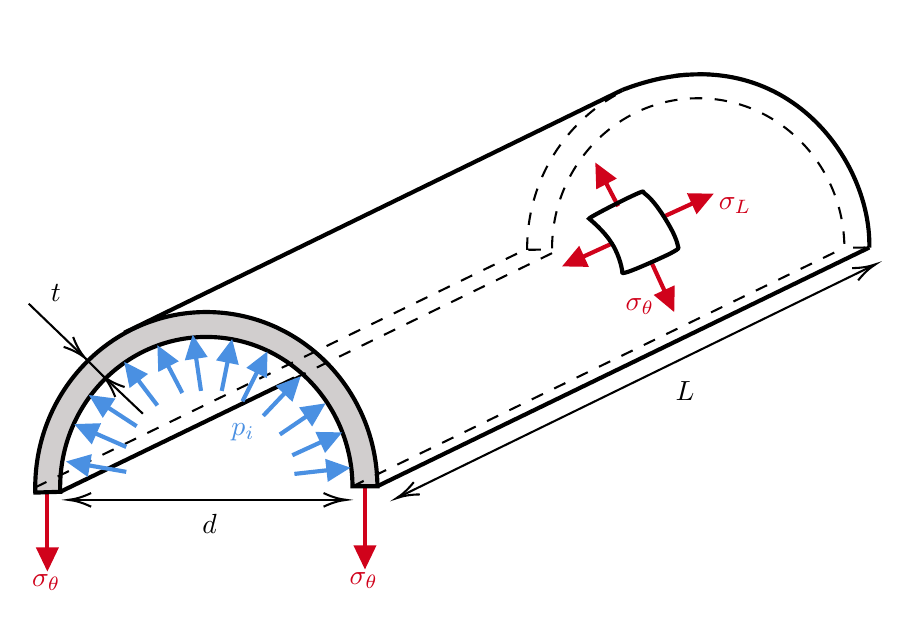
\begin{tikzpicture}[x=0.75pt,y=0.75pt,yscale=-1,xscale=1]
		%uncomment if require: \path (0,656); %set diagram left start at 0, and has height of 656
		
		%Straight Lines [id:da23681895937591246] 
		\draw [color={rgb, 255:red, 208; green, 2; blue, 27 }  ,draw opacity=1 ][line width=1.5]    (156.86,256.28) -- (156.86,291.28) ;
		\draw [shift={(156.86,295.28)}, rotate = 270] [fill={rgb, 255:red, 208; green, 2; blue, 27 }  ,fill opacity=1 ][line width=0.08]  [draw opacity=0] (11.61,-5.58) -- (0,0) -- (11.61,5.58) -- cycle    ;
		%Straight Lines [id:da4211597130223663] 
		\draw [color={rgb, 255:red, 208; green, 2; blue, 27 }  ,draw opacity=1 ][line width=1.5]    (309.86,255.28) -- (309.86,290.28) ;
		\draw [shift={(309.86,294.28)}, rotate = 270] [fill={rgb, 255:red, 208; green, 2; blue, 27 }  ,fill opacity=1 ][line width=0.08]  [draw opacity=0] (11.61,-5.58) -- (0,0) -- (11.61,5.58) -- cycle    ;
		%Shape: Block Arc [id:dp6997906607111268] 
		\draw  [fill={rgb, 255:red, 209; green, 206; blue, 206 }  ,fill opacity=1 ][line width=1.5]  (151.04,257.27) .. controls (151.01,256.44) and (151,255.61) .. (151,254.78) .. controls (151,208.11) and (187.91,170.28) .. (233.43,170.28) .. controls (278.77,170.28) and (315.55,207.79) .. (315.86,254.19) -- (303.86,254.27) .. controls (303.6,214.46) and (272.17,182.28) .. (233.43,182.28) .. controls (194.53,182.28) and (163,214.74) .. (163,254.78) .. controls (163,255.49) and (163.01,256.2) .. (163.03,256.9) -- cycle ;
		%Straight Lines [id:da753088895429614] 
		\draw [line width=1.5]    (193.86,180.28) -- (433.86,63.28) ;
		%Straight Lines [id:da7155061779490777] 
		\draw [line width=1.5]    (315.86,254.19) -- (552.86,139.19) ;
		%Curve Lines [id:da877206751683749] 
		\draw [line width=1.5]    (433.86,63.28) .. controls (508.86,34.28) and (553.86,95.28) .. (552.86,139.19) ;
		%Shape: Block Arc [id:dp12907430395390063] 
		\draw  [dash pattern={on 4.5pt off 4.5pt}][line width=0.75]  (388,140.28) .. controls (388,140.11) and (388,139.95) .. (388,139.78) .. controls (388,93.11) and (424.91,55.28) .. (470.43,55.28) .. controls (515.77,55.28) and (552.55,92.79) .. (552.86,139.19) -- (540.86,139.27) .. controls (540.6,99.46) and (509.17,67.28) .. (470.43,67.28) .. controls (431.53,67.28) and (400,99.74) .. (400,139.78) .. controls (400,139.92) and (400,140.07) .. (400,140.21) -- cycle ;
		%Straight Lines [id:da8437245732626601] 
		\draw [line width=0.75]  [dash pattern={on 4.5pt off 4.5pt}]  (303.86,254.27) -- (444.67,185.95) -- (540.86,139.27) ;
		%Straight Lines [id:da5251843894923394] 
		\draw [line width=0.75]  [dash pattern={on 4.5pt off 4.5pt}]  (151,254.78) -- (388,139.78) ;
		%Straight Lines [id:da5535958795398617] 
		\draw [line width=0.75]  [dash pattern={on 4.5pt off 4.5pt}]  (275.86,202.28) -- (400.03,141.9) ;
		%Straight Lines [id:da9442398167575681] 
		\draw [line width=1.5]    (163.03,256.9) -- (275.86,202.28) ;
		%Straight Lines [id:da9749005033770579] 
		\draw    (326.8,259.12) -- (554.07,148.16) ;
		\draw [shift={(555.86,147.28)}, rotate = 153.98] [color={rgb, 255:red, 0; green, 0; blue, 0 }  ][line width=0.75]    (10.93,-3.29) .. controls (6.95,-1.4) and (3.31,-0.3) .. (0,0) .. controls (3.31,0.3) and (6.95,1.4) .. (10.93,3.29)   ;
		\draw [shift={(325,260)}, rotate = 333.98] [color={rgb, 255:red, 0; green, 0; blue, 0 }  ][line width=0.75]    (10.93,-3.29) .. controls (6.95,-1.4) and (3.31,-0.3) .. (0,0) .. controls (3.31,0.3) and (6.95,1.4) .. (10.93,3.29)   ;
		%Straight Lines [id:da7918954694053384] 
		\draw    (169,260.78) -- (298.86,260.78) ;
		\draw [shift={(300.86,260.78)}, rotate = 180] [color={rgb, 255:red, 0; green, 0; blue, 0 }  ][line width=0.75]    (10.93,-3.29) .. controls (6.95,-1.4) and (3.31,-0.3) .. (0,0) .. controls (3.31,0.3) and (6.95,1.4) .. (10.93,3.29)   ;
		\draw [shift={(167,260.78)}, rotate = 0] [color={rgb, 255:red, 0; green, 0; blue, 0 }  ][line width=0.75]    (10.93,-3.29) .. controls (6.95,-1.4) and (3.31,-0.3) .. (0,0) .. controls (3.31,0.3) and (6.95,1.4) .. (10.93,3.29)   ;
		%Straight Lines [id:da05784248120983948] 
		\draw    (147.86,166.28) -- (173.42,190.89) ;
		\draw [shift={(174.86,192.28)}, rotate = 223.92] [color={rgb, 255:red, 0; green, 0; blue, 0 }  ][line width=0.75]    (10.93,-3.29) .. controls (6.95,-1.4) and (3.31,-0.3) .. (0,0) .. controls (3.31,0.3) and (6.95,1.4) .. (10.93,3.29)   ;
		%Straight Lines [id:da881729698435544] 
		\draw    (202.86,219.28) -- (185.32,202.65) ;
		\draw [shift={(183.86,201.28)}, rotate = 43.45] [color={rgb, 255:red, 0; green, 0; blue, 0 }  ][line width=0.75]    (10.93,-3.29) .. controls (6.95,-1.4) and (3.31,-0.3) .. (0,0) .. controls (3.31,0.3) and (6.95,1.4) .. (10.93,3.29)   ;
		%Straight Lines [id:da40970785578528646] 
		\draw    (174.86,192.28) -- (183.86,201.28) ;
		%Straight Lines [id:da21182349489015073] 
		\draw [color={rgb, 255:red, 208; green, 2; blue, 27 }  ,draw opacity=1 ][line width=1.5]    (447.86,146.28) -- (457.2,166.64) ;
		\draw [shift={(458.86,170.28)}, rotate = 245.38] [fill={rgb, 255:red, 208; green, 2; blue, 27 }  ,fill opacity=1 ][line width=0.08]  [draw opacity=0] (11.61,-5.58) -- (0,0) -- (11.61,5.58) -- cycle    ;
		%Straight Lines [id:da6698414615655965] 
		\draw [color={rgb, 255:red, 208; green, 2; blue, 27 }  ,draw opacity=1 ][line width=1.5]    (453.86,124.28) -- (474.23,114.95) ;
		\draw [shift={(477.86,113.28)}, rotate = 155.38] [fill={rgb, 255:red, 208; green, 2; blue, 27 }  ,fill opacity=1 ][line width=0.08]  [draw opacity=0] (11.61,-5.58) -- (0,0) -- (11.61,5.58) -- cycle    ;
		%Straight Lines [id:da3508347268612697] 
		\draw [color={rgb, 255:red, 208; green, 2; blue, 27 }  ,draw opacity=1 ][line width=1.5]    (428.86,137.28) -- (408.5,146.61) ;
		\draw [shift={(404.86,148.28)}, rotate = 335.38] [fill={rgb, 255:red, 208; green, 2; blue, 27 }  ,fill opacity=1 ][line width=0.08]  [draw opacity=0] (11.61,-5.58) -- (0,0) -- (11.61,5.58) -- cycle    ;
		%Straight Lines [id:da6576025598874233] 
		\draw [color={rgb, 255:red, 208; green, 2; blue, 27 }  ,draw opacity=1 ][line width=1.5]    (431.86,119.28) -- (422.72,101.82) ;
		\draw [shift={(420.86,98.28)}, rotate = 62.35] [fill={rgb, 255:red, 208; green, 2; blue, 27 }  ,fill opacity=1 ][line width=0.08]  [draw opacity=0] (11.61,-5.58) -- (0,0) -- (11.61,5.58) -- cycle    ;
		%Shape: Polygon Curved [id:ds04449597420019402] 
		\draw  [line width=1.5]  (417.86,125.28) .. controls (417.38,124.79) and (443.86,111.28) .. (443.86,112.28) .. controls (443.86,113.28) and (446.86,113.28) .. (453.86,124.28) .. controls (460.86,135.28) and (460.38,138.32) .. (460.86,139.28) .. controls (461.34,140.24) and (454.36,143.39) .. (447.86,146.28) .. controls (441.36,149.17) and (433.86,152.33) .. (433.86,151.28) .. controls (433.86,150.23) and (432.83,143.66) .. (428.86,137.28) .. controls (424.9,130.9) and (418.35,125.77) .. (417.86,125.28) -- cycle ;
		%Straight Lines [id:da2879699025804068] 
		\draw [color={rgb, 255:red, 74; green, 144; blue, 226 }  ,draw opacity=1 ][line width=1.5]    (194.86,247.28) -- (169.81,242.96) ;
		\draw [shift={(165.86,242.28)}, rotate = 9.78] [fill={rgb, 255:red, 74; green, 144; blue, 226 }  ,fill opacity=1 ][line width=0.08]  [draw opacity=0] (11.61,-5.58) -- (0,0) -- (11.61,5.58) -- cycle    ;
		%Straight Lines [id:da5590321039654371] 
		\draw [color={rgb, 255:red, 74; green, 144; blue, 226 }  ,draw opacity=1 ][line width=1.5]    (194.86,235.28) -- (173.52,225.89) ;
		\draw [shift={(169.86,224.28)}, rotate = 23.75] [fill={rgb, 255:red, 74; green, 144; blue, 226 }  ,fill opacity=1 ][line width=0.08]  [draw opacity=0] (11.61,-5.58) -- (0,0) -- (11.61,5.58) -- cycle    ;
		%Straight Lines [id:da17255463038436925] 
		\draw [color={rgb, 255:red, 74; green, 144; blue, 226 }  ,draw opacity=1 ][line width=1.5]    (199.86,225.28) -- (180.21,212.46) ;
		\draw [shift={(176.86,210.28)}, rotate = 33.11] [fill={rgb, 255:red, 74; green, 144; blue, 226 }  ,fill opacity=1 ][line width=0.08]  [draw opacity=0] (11.61,-5.58) -- (0,0) -- (11.61,5.58) -- cycle    ;
		%Straight Lines [id:da381265282603787] 
		\draw [color={rgb, 255:red, 74; green, 144; blue, 226 }  ,draw opacity=1 ][line width=1.5]    (209.86,215.28) -- (196.29,197.46) ;
		\draw [shift={(193.86,194.28)}, rotate = 52.7] [fill={rgb, 255:red, 74; green, 144; blue, 226 }  ,fill opacity=1 ][line width=0.08]  [draw opacity=0] (11.61,-5.58) -- (0,0) -- (11.61,5.58) -- cycle    ;
		%Straight Lines [id:da048912956022172605] 
		\draw [color={rgb, 255:red, 74; green, 144; blue, 226 }  ,draw opacity=1 ][line width=1.5]    (221.86,209.28) -- (211.71,189.82) ;
		\draw [shift={(209.86,186.28)}, rotate = 62.45] [fill={rgb, 255:red, 74; green, 144; blue, 226 }  ,fill opacity=1 ][line width=0.08]  [draw opacity=0] (11.61,-5.58) -- (0,0) -- (11.61,5.58) -- cycle    ;
		%Straight Lines [id:da5652522396268675] 
		\draw [color={rgb, 255:red, 74; green, 144; blue, 226 }  ,draw opacity=1 ][line width=1.5]    (230.86,208.28) -- (227.45,185.24) ;
		\draw [shift={(226.86,181.28)}, rotate = 81.57] [fill={rgb, 255:red, 74; green, 144; blue, 226 }  ,fill opacity=1 ][line width=0.08]  [draw opacity=0] (11.61,-5.58) -- (0,0) -- (11.61,5.58) -- cycle    ;
		%Straight Lines [id:da1354377144947716] 
		\draw [color={rgb, 255:red, 74; green, 144; blue, 226 }  ,draw opacity=1 ][line width=1.5]    (240.86,208.28) -- (245.08,187.2) ;
		\draw [shift={(245.86,183.28)}, rotate = 101.31] [fill={rgb, 255:red, 74; green, 144; blue, 226 }  ,fill opacity=1 ][line width=0.08]  [draw opacity=0] (11.61,-5.58) -- (0,0) -- (11.61,5.58) -- cycle    ;
		%Straight Lines [id:da23988365211989526] 
		\draw [color={rgb, 255:red, 74; green, 144; blue, 226 }  ,draw opacity=1 ][line width=1.5]    (250.86,213.28) -- (261.07,192.86) ;
		\draw [shift={(262.86,189.28)}, rotate = 116.57] [fill={rgb, 255:red, 74; green, 144; blue, 226 }  ,fill opacity=1 ][line width=0.08]  [draw opacity=0] (11.61,-5.58) -- (0,0) -- (11.61,5.58) -- cycle    ;
		%Straight Lines [id:da23754603110345718] 
		\draw [color={rgb, 255:red, 74; green, 144; blue, 226 }  ,draw opacity=1 ][line width=1.5]    (260.86,220.28) -- (276.11,204.18) ;
		\draw [shift={(278.86,201.28)}, rotate = 133.45] [fill={rgb, 255:red, 74; green, 144; blue, 226 }  ,fill opacity=1 ][line width=0.08]  [draw opacity=0] (11.61,-5.58) -- (0,0) -- (11.61,5.58) -- cycle    ;
		%Straight Lines [id:da6298334600737221] 
		\draw [color={rgb, 255:red, 74; green, 144; blue, 226 }  ,draw opacity=1 ][line width=1.5]    (268.86,229.28) -- (287.56,216.53) ;
		\draw [shift={(290.86,214.28)}, rotate = 145.71] [fill={rgb, 255:red, 74; green, 144; blue, 226 }  ,fill opacity=1 ][line width=0.08]  [draw opacity=0] (11.61,-5.58) -- (0,0) -- (11.61,5.58) -- cycle    ;
		%Straight Lines [id:da47170882754369625] 
		\draw [color={rgb, 255:red, 74; green, 144; blue, 226 }  ,draw opacity=1 ][line width=1.5]    (274.86,239.28) -- (295.23,229.95) ;
		\draw [shift={(298.86,228.28)}, rotate = 155.38] [fill={rgb, 255:red, 74; green, 144; blue, 226 }  ,fill opacity=1 ][line width=0.08]  [draw opacity=0] (11.61,-5.58) -- (0,0) -- (11.61,5.58) -- cycle    ;
		%Straight Lines [id:da6330787889962182] 
		\draw [color={rgb, 255:red, 74; green, 144; blue, 226 }  ,draw opacity=1 ][line width=1.5]    (275.86,248.28) -- (298.89,245.72) ;
		\draw [shift={(302.86,245.28)}, rotate = 173.66] [fill={rgb, 255:red, 74; green, 144; blue, 226 }  ,fill opacity=1 ][line width=0.08]  [draw opacity=0] (11.61,-5.58) -- (0,0) -- (11.61,5.58) -- cycle    ;
		
		% Text Node
		\draw (458,202.4) node [anchor=north west][inner sep=0.75pt]    {$L$};
		% Text Node
		\draw (230,266.4) node [anchor=north west][inner sep=0.75pt]    {$d$};
		% Text Node
		\draw (157,155.4) node [anchor=north west][inner sep=0.75pt]    {$t$};
		% Text Node
		\draw (148,295.4) node [anchor=north west][inner sep=0.75pt]  [color={rgb, 255:red, 208; green, 2; blue, 27 }  ,opacity=1 ]  {$\sigma _{\theta }$};
		% Text Node
		\draw (301,294.4) node [anchor=north west][inner sep=0.75pt]  [color={rgb, 255:red, 208; green, 2; blue, 27 }  ,opacity=1 ]  {$\sigma _{\theta }$};
		% Text Node
		\draw (434,162.4) node [anchor=north west][inner sep=0.75pt]  [color={rgb, 255:red, 208; green, 2; blue, 27 }  ,opacity=1 ]  {$\sigma _{\theta }$};
		% Text Node
		\draw (478.86,113.68) node [anchor=north west][inner sep=0.75pt]  [color={rgb, 255:red, 208; green, 2; blue, 27 }  ,opacity=1 ]  {$\sigma _{L}$};
		% Text Node
		\draw (244,222.4) node [anchor=north west][inner sep=0.75pt]  [color={rgb, 255:red, 74; green, 144; blue, 226 }  ,opacity=1 ]  {$p_{i}$};
		\end{tikzpicture}
	\end{figure}
	The total force on half of the cylinder due to the internal pressure is given by thanks to the symmetry of geometry:
	
	The total resisting force due to the hoop stress, $\sigma_\theta$, established in the cylinder walls is given by:
	
	Equating these:
	
	Therefore we get for the hoop stress of a thin cylinder:
	
	The expression rearranged as following (and with a change of notation $p_i=P$):
	
	is quite famous and known as "\NewTerm{Barlow's formula}\index{Barlow's formula}" (for Peter Barlow in 11817 according to holocene calendar) or very rarely "Mariotte's formula" (not to be confused with the formula of the same name in compressed gases theory!). In reality the current shape Barlow’s formula above has been obtained by John Goodman in his textbook \textit{Mechanics applied to Engineering} (in 11914 according to holocene calendar).
	
	This formula (DIN 2413) figures prominently in the design of autoclaves and other pressure vessels!
	\begin{figure}[H]
		\centering
		\includegraphics[scale=0.9]{img/engineering/vessel_gaz_bottle.jpg}
	\end{figure}
	
	\begin{tcolorbox}[enhanced,title=Remarks,colframe=black,arc=10pt,drop lifted shadow,after skip=15pt plus 2pt]
	\textbf{R1.} The Barlow’s formula with the mean diameter leads to the "Boardman’s formula" which is basic for the rules of all pressure vessels and piping design codes.\\
	
	\textbf{R2.} The Barlow’s formula with the ultimate tensile strength and the mean diameter gives reliable values for the collapse (bursting) pressure of piping made with steels having strain hardening exponent  (carbon steels); on the contrary, it cannot be applied to steels having high strain hardening exponent, as austenitic stainless steels.
	\end{tcolorbox}
	
	\subparagraph{Longitudinal stress $\sigma_L$}\mbox{}\\\\
	Consider the cross section of a thin cylinder as shown below (ending like a gas cylinder):
	\begin{figure}[H]
		\centering
		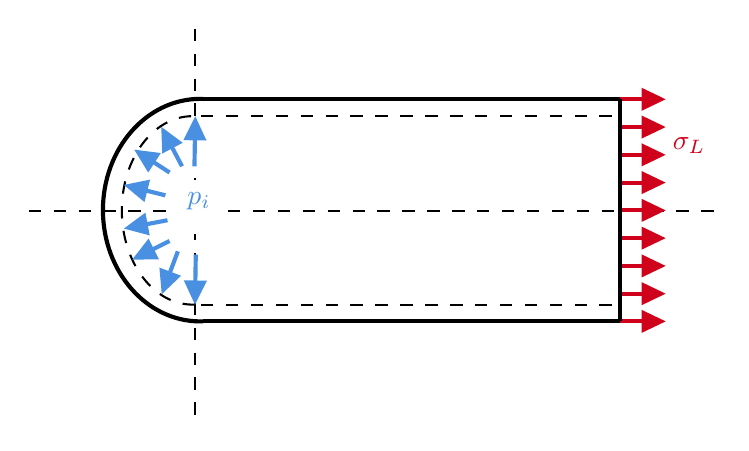
\begin{tikzpicture}[x=0.75pt,y=0.75pt,yscale=-1,xscale=1]
		%uncomment if require: \path (0,578); %set diagram left start at 0, and has height of 578
		
		%Straight Lines [id:da3649300081294653] 
		\draw  [dash pattern={on 4.5pt off 4.5pt}]  (130,123) -- (462.86,123) ;
		%Straight Lines [id:da1880005535965441] 
		\draw [color={rgb, 255:red, 208; green, 2; blue, 27 }  ,draw opacity=1 ][line width=1.5]    (413.86,69) -- (432.86,69) ;
		\draw [shift={(436.86,69)}, rotate = 180] [fill={rgb, 255:red, 208; green, 2; blue, 27 }  ,fill opacity=1 ][line width=0.08]  [draw opacity=0] (11.61,-5.58) -- (0,0) -- (11.61,5.58) -- cycle    ;
		%Straight Lines [id:da22332119437173592] 
		\draw [color={rgb, 255:red, 208; green, 2; blue, 27 }  ,draw opacity=1 ][line width=1.5]    (413.86,176) -- (432.86,176) ;
		\draw [shift={(436.86,176)}, rotate = 180] [fill={rgb, 255:red, 208; green, 2; blue, 27 }  ,fill opacity=1 ][line width=0.08]  [draw opacity=0] (11.61,-5.58) -- (0,0) -- (11.61,5.58) -- cycle    ;
		%Straight Lines [id:da8331946627230009] 
		\draw [color={rgb, 255:red, 208; green, 2; blue, 27 }  ,draw opacity=1 ][line width=1.5]    (413.86,162.66) -- (432.86,162.66) ;
		\draw [shift={(436.86,162.66)}, rotate = 180] [fill={rgb, 255:red, 208; green, 2; blue, 27 }  ,fill opacity=1 ][line width=0.08]  [draw opacity=0] (11.61,-5.58) -- (0,0) -- (11.61,5.58) -- cycle    ;
		%Straight Lines [id:da2314442918093529] 
		\draw [color={rgb, 255:red, 208; green, 2; blue, 27 }  ,draw opacity=1 ][line width=1.5]    (413.86,149.28) -- (432.86,149.28) ;
		\draw [shift={(436.86,149.28)}, rotate = 180] [fill={rgb, 255:red, 208; green, 2; blue, 27 }  ,fill opacity=1 ][line width=0.08]  [draw opacity=0] (11.61,-5.58) -- (0,0) -- (11.61,5.58) -- cycle    ;
		%Straight Lines [id:da002566207402936671] 
		\draw [color={rgb, 255:red, 208; green, 2; blue, 27 }  ,draw opacity=1 ][line width=1.5]    (413.86,135.9) -- (432.86,135.9) ;
		\draw [shift={(436.86,135.9)}, rotate = 180] [fill={rgb, 255:red, 208; green, 2; blue, 27 }  ,fill opacity=1 ][line width=0.08]  [draw opacity=0] (11.61,-5.58) -- (0,0) -- (11.61,5.58) -- cycle    ;
		%Straight Lines [id:da3774242289230598] 
		\draw [color={rgb, 255:red, 208; green, 2; blue, 27 }  ,draw opacity=1 ][line width=1.5]    (413.86,122.52) -- (432.86,122.52) ;
		\draw [shift={(436.86,122.52)}, rotate = 180] [fill={rgb, 255:red, 208; green, 2; blue, 27 }  ,fill opacity=1 ][line width=0.08]  [draw opacity=0] (11.61,-5.58) -- (0,0) -- (11.61,5.58) -- cycle    ;
		%Straight Lines [id:da0507602302226855] 
		\draw [color={rgb, 255:red, 208; green, 2; blue, 27 }  ,draw opacity=1 ][line width=1.5]    (413.86,109.14) -- (432.86,109.14) ;
		\draw [shift={(436.86,109.14)}, rotate = 180] [fill={rgb, 255:red, 208; green, 2; blue, 27 }  ,fill opacity=1 ][line width=0.08]  [draw opacity=0] (11.61,-5.58) -- (0,0) -- (11.61,5.58) -- cycle    ;
		%Straight Lines [id:da18452841079332605] 
		\draw [color={rgb, 255:red, 208; green, 2; blue, 27 }  ,draw opacity=1 ][line width=1.5]    (413.86,95.76) -- (432.86,95.76) ;
		\draw [shift={(436.86,95.76)}, rotate = 180] [fill={rgb, 255:red, 208; green, 2; blue, 27 }  ,fill opacity=1 ][line width=0.08]  [draw opacity=0] (11.61,-5.58) -- (0,0) -- (11.61,5.58) -- cycle    ;
		%Straight Lines [id:da637725515335158] 
		\draw [color={rgb, 255:red, 208; green, 2; blue, 27 }  ,draw opacity=1 ][line width=1.5]    (413.86,82.38) -- (432.86,82.38) ;
		\draw [shift={(436.86,82.38)}, rotate = 180] [fill={rgb, 255:red, 208; green, 2; blue, 27 }  ,fill opacity=1 ][line width=0.08]  [draw opacity=0] (11.61,-5.58) -- (0,0) -- (11.61,5.58) -- cycle    ;
		%Straight Lines [id:da9933383388785164] 
		\draw [line width=1.5]    (214,69) -- (414.86,69) ;
		%Straight Lines [id:da7708456113621964] 
		\draw [line width=1.5]    (214,176) -- (414.86,176) ;
		%Straight Lines [id:da6971319892652692] 
		\draw [line width=1.5]    (414.86,69) -- (414.86,176) ;
		%Shape: Arc [id:dp6131450871694619] 
		\draw  [draw opacity=0][line width=1.5]  (214,176) .. controls (213.54,176.02) and (213.08,176.02) .. (212.62,176.02) .. controls (186.74,176.02) and (165.76,152.02) .. (165.76,122.41) .. controls (165.76,92.81) and (186.74,68.8) .. (212.62,68.8) .. controls (213.14,68.8) and (213.65,68.81) .. (214.17,68.83) -- (212.62,122.41) -- cycle ; \draw  [line width=1.5]  (214,176) .. controls (213.54,176.02) and (213.08,176.02) .. (212.62,176.02) .. controls (186.74,176.02) and (165.76,152.02) .. (165.76,122.41) .. controls (165.76,92.81) and (186.74,68.8) .. (212.62,68.8) .. controls (213.14,68.8) and (213.65,68.81) .. (214.17,68.83) ;  
		%Straight Lines [id:da7910760879787793] 
		\draw  [dash pattern={on 4.5pt off 4.5pt}]  (210,35) -- (210,224.28) ;
		%Straight Lines [id:da06042752706044574] 
		\draw [line width=0.75]  [dash pattern={on 4.5pt off 4.5pt}]  (213,77) -- (413.86,77) ;
		%Straight Lines [id:da0007388934683603132] 
		\draw [line width=0.75]  [dash pattern={on 4.5pt off 4.5pt}]  (213,168) -- (413.86,168) ;
		%Shape: Arc [id:dp25505742768017514] 
		\draw  [draw opacity=0][dash pattern={on 4.5pt off 4.5pt}][line width=0.75]  (210.1,167.91) .. controls (209.71,167.92) and (209.32,167.93) .. (208.93,167.93) .. controls (190.12,167.93) and (174.86,147.61) .. (174.86,122.53) .. controls (174.86,97.46) and (190.12,77.13) .. (208.93,77.13) .. controls (209.37,77.13) and (209.81,77.14) .. (210.25,77.17) -- (208.93,122.53) -- cycle ; \draw  [dash pattern={on 4.5pt off 4.5pt}][line width=0.75]  (210.1,167.91) .. controls (209.71,167.92) and (209.32,167.93) .. (208.93,167.93) .. controls (190.12,167.93) and (174.86,147.61) .. (174.86,122.53) .. controls (174.86,97.46) and (190.12,77.13) .. (208.93,77.13) .. controls (209.37,77.13) and (209.81,77.14) .. (210.25,77.17) ;  
		%Straight Lines [id:da8559045041155136] 
		\draw [color={rgb, 255:red, 74; green, 144; blue, 226 }  ,draw opacity=1 ][line width=1.5]    (209.86,101.28) -- (210.18,81.17) ;
		\draw [shift={(210.25,77.17)}, rotate = 90.91] [fill={rgb, 255:red, 74; green, 144; blue, 226 }  ,fill opacity=1 ][line width=0.08]  [draw opacity=0] (11.61,-5.58) -- (0,0) -- (11.61,5.58) -- cycle    ;
		%Straight Lines [id:da5516483088336146] 
		\draw [color={rgb, 255:red, 74; green, 144; blue, 226 }  ,draw opacity=1 ][line width=1.5]    (210.49,143.79) -- (210.17,163.91) ;
		\draw [shift={(210.1,167.91)}, rotate = 270.91] [fill={rgb, 255:red, 74; green, 144; blue, 226 }  ,fill opacity=1 ][line width=0.08]  [draw opacity=0] (11.61,-5.58) -- (0,0) -- (11.61,5.58) -- cycle    ;
		%Straight Lines [id:da7266635848237712] 
		\draw [color={rgb, 255:red, 74; green, 144; blue, 226 }  ,draw opacity=1 ][line width=1.5]    (201.86,142.28) -- (195.51,159.16) ;
		\draw [shift={(194.1,162.91)}, rotate = 290.61] [fill={rgb, 255:red, 74; green, 144; blue, 226 }  ,fill opacity=1 ][line width=0.08]  [draw opacity=0] (11.61,-5.58) -- (0,0) -- (11.61,5.58) -- cycle    ;
		%Straight Lines [id:da7147413447431774] 
		\draw [color={rgb, 255:red, 74; green, 144; blue, 226 }  ,draw opacity=1 ][line width=1.5]    (197.86,137.28) -- (183.44,144.49) ;
		\draw [shift={(179.86,146.28)}, rotate = 333.43] [fill={rgb, 255:red, 74; green, 144; blue, 226 }  ,fill opacity=1 ][line width=0.08]  [draw opacity=0] (11.61,-5.58) -- (0,0) -- (11.61,5.58) -- cycle    ;
		%Straight Lines [id:da6893552746754228] 
		\draw [color={rgb, 255:red, 74; green, 144; blue, 226 }  ,draw opacity=1 ][line width=1.5]    (196.86,127.28) -- (179.79,130.53) ;
		\draw [shift={(175.86,131.28)}, rotate = 349.22] [fill={rgb, 255:red, 74; green, 144; blue, 226 }  ,fill opacity=1 ][line width=0.08]  [draw opacity=0] (11.61,-5.58) -- (0,0) -- (11.61,5.58) -- cycle    ;
		%Straight Lines [id:da18575080555945034] 
		\draw [color={rgb, 255:red, 74; green, 144; blue, 226 }  ,draw opacity=1 ][line width=1.5]    (195.86,115.28) -- (179.74,111.25) ;
		\draw [shift={(175.86,110.28)}, rotate = 14.04] [fill={rgb, 255:red, 74; green, 144; blue, 226 }  ,fill opacity=1 ][line width=0.08]  [draw opacity=0] (11.61,-5.58) -- (0,0) -- (11.61,5.58) -- cycle    ;
		%Straight Lines [id:da7101869500756737] 
		\draw [color={rgb, 255:red, 74; green, 144; blue, 226 }  ,draw opacity=1 ][line width=1.5]    (197.86,104.28) -- (184.22,95.45) ;
		\draw [shift={(180.86,93.28)}, rotate = 32.91] [fill={rgb, 255:red, 74; green, 144; blue, 226 }  ,fill opacity=1 ][line width=0.08]  [draw opacity=0] (11.61,-5.58) -- (0,0) -- (11.61,5.58) -- cycle    ;
		%Straight Lines [id:da3612068289973456] 
		\draw [color={rgb, 255:red, 74; green, 144; blue, 226 }  ,draw opacity=1 ][line width=1.5]    (203.86,101.28) -- (195.73,85.82) ;
		\draw [shift={(193.86,82.28)}, rotate = 62.24] [fill={rgb, 255:red, 74; green, 144; blue, 226 }  ,fill opacity=1 ][line width=0.08]  [draw opacity=0] (11.61,-5.58) -- (0,0) -- (11.61,5.58) -- cycle    ;
		
		% Text Node
		\draw (438.86,85.78) node [anchor=north west][inner sep=0.75pt]  [color={rgb, 255:red, 208; green, 2; blue, 27 }  ,opacity=1 ]  {$\sigma _{L}$};
		% Text Node
		\draw  [draw opacity=0][fill={rgb, 255:red, 255; green, 255; blue, 255 }  ,fill opacity=1 ]  (202,108) -- (223,108) -- (223,134) -- (202,134) -- cycle  ;
		\draw (205,112.4) node [anchor=north west][inner sep=0.75pt]  [color={rgb, 255:red, 74; green, 144; blue, 226 }  ,opacity=1 ]  {$p_{i}$};
		\end{tikzpicture}
	\end{figure}
	The total force acting on the end of the cylinder due to the internal pressure is given by (don't forget that the end of the cylinder are considered a half sphere here):
	
	The total resisting force due to the axial (longitudinal) stress, $\sigma_L$, established in the cylinder walls extremities (two half balls of radius $r$) is given by :
	
	Equating these:
	
	Therefore we get for the longitudinal (axial) stress of a thin cylinder:
	
	Surprisingly the result for a cylinder that ends with a flat disc rather than a half sphere is the same as the project area is equal.
	
	Notice that:
	
	
	\begin{figure}[H]
		\centering
		\includegraphics[scale=0.5]{img/engineering/vessel_gaz.jpg}
	\end{figure}
	
	\begin{tcolorbox}[colframe=black,colback=white,sharp corners,breakable]
	\textbf{{\Large \ding{45}}Example:}\\\\
	Consider the typical International Space Station (ISS) module cylinder of $13.7$ meters long (ending with flat discs), with a $1.9$ meter internal diameter with walls $4$ millimetres thick (all values are real and taken from NASA website) is subjected to an internal pressure of $1$ atmosphere (i.e. $101.3\cdot 10^3\;[\text{N}\cdot\text{m}^{-2}]$). We have therefore:
	$$\sigma_\theta=\dfrac{p_i d}{2t}=\dfrac{(101.3\cdot 10^3) \cdot 1.9 }{2\cdot 4\cdot 10^{-3}}=24.1\;[\text{MN}\cdot\text{m}^{-2}]$$
	and:
	$$\sigma_L=\dfrac{p_i d}{4t}=\dfrac{(101.3\cdot 10^3) \cdot 1.9 }{2\cdot 4\cdot 10^{-3}}=12.03\;[\text{MN}\cdot\text{m}^{-2}]$$
	\begin{figure}[H]
		\centering
		\includegraphics[scale=0.7]{img/engineering/iss_module.jpeg}
	\end{figure}
	Most ISS modules are made of 2219 aluminium alloy whose tensile strength is $172$ to $476 \;[\text{MN}\cdot\text{m}^{-2}]$.
	\end{tcolorbox}
	
	\paragraph{Thin sphere subjected to internal pressure}\mbox{}\\\\
	Deriving stresses in the walls of a spherical container is very similar to cylindrical containers. Consider the half section of the spherical container shown in in the figure below:
	\begin{figure}[H]
		\centering
		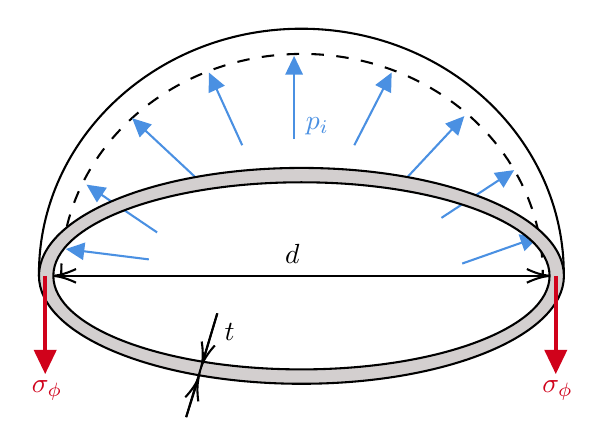
\begin{tikzpicture}[x=0.75pt,y=0.75pt,yscale=-1,xscale=1]
		%uncomment if require: \path (0,484); %set diagram left start at 0, and has height of 484
		
		%Shape: Arc [id:dp8000187239175336] 
		\draw  [draw opacity=0][dash pattern={on 4.5pt off 4.5pt}] (191.67,174.25) .. controls (191.67,173.93) and (191.67,173.6) .. (191.67,173.28) .. controls (191.67,114.74) and (243.6,67.28) .. (307.67,67.28) .. controls (371.73,67.28) and (423.67,114.74) .. (423.67,173.28) .. controls (423.67,173.32) and (423.67,173.36) .. (423.67,173.4) -- (307.67,173.28) -- cycle ; \draw  [dash pattern={on 4.5pt off 4.5pt}] (191.67,174.25) .. controls (191.67,173.93) and (191.67,173.6) .. (191.67,173.28) .. controls (191.67,114.74) and (243.6,67.28) .. (307.67,67.28) .. controls (371.73,67.28) and (423.67,114.74) .. (423.67,173.28) .. controls (423.67,173.32) and (423.67,173.36) .. (423.67,173.4) ;  
		%Shape: Arc [id:dp26418344222128587] 
		\draw  [draw opacity=0] (180.94,174.21) .. controls (180.93,173.9) and (180.93,173.59) .. (180.93,173.28) .. controls (180.93,108.03) and (237.54,55.14) .. (307.36,55.14) .. controls (377.19,55.14) and (433.8,108.03) .. (433.8,173.28) .. controls (433.8,173.32) and (433.8,173.37) .. (433.8,173.41) -- (307.36,173.28) -- cycle ; \draw   (180.94,174.21) .. controls (180.93,173.9) and (180.93,173.59) .. (180.93,173.28) .. controls (180.93,108.03) and (237.54,55.14) .. (307.36,55.14) .. controls (377.19,55.14) and (433.8,108.03) .. (433.8,173.28) .. controls (433.8,173.32) and (433.8,173.37) .. (433.8,173.41) ;  
		%Straight Lines [id:da9458683600790103] 
		\draw    (189.86,174.21) -- (424.94,174.21) ;
		\draw [shift={(426.94,174.21)}, rotate = 180] [color={rgb, 255:red, 0; green, 0; blue, 0 }  ][line width=0.75]    (10.93,-3.29) .. controls (6.95,-1.4) and (3.31,-0.3) .. (0,0) .. controls (3.31,0.3) and (6.95,1.4) .. (10.93,3.29)   ;
		\draw [shift={(187.86,174.21)}, rotate = 0] [color={rgb, 255:red, 0; green, 0; blue, 0 }  ][line width=0.75]    (10.93,-3.29) .. controls (6.95,-1.4) and (3.31,-0.3) .. (0,0) .. controls (3.31,0.3) and (6.95,1.4) .. (10.93,3.29)   ;
		%Straight Lines [id:da5644772342341278] 
		\draw [color={rgb, 255:red, 74; green, 144; blue, 226 }  ,draw opacity=1 ]   (237.86,153.28) -- (206.35,131.96) ;
		\draw [shift={(203.86,130.28)}, rotate = 34.08] [fill={rgb, 255:red, 74; green, 144; blue, 226 }  ,fill opacity=1 ][line width=0.08]  [draw opacity=0] (8.93,-4.29) -- (0,0) -- (8.93,4.29) -- cycle    ;
		%Straight Lines [id:da9901018543139823] 
		\draw [color={rgb, 255:red, 74; green, 144; blue, 226 }  ,draw opacity=1 ]   (255.86,126.28) -- (228.06,100.33) ;
		\draw [shift={(225.86,98.28)}, rotate = 43.03] [fill={rgb, 255:red, 74; green, 144; blue, 226 }  ,fill opacity=1 ][line width=0.08]  [draw opacity=0] (8.93,-4.29) -- (0,0) -- (8.93,4.29) -- cycle    ;
		%Straight Lines [id:da8861016334435436] 
		\draw [color={rgb, 255:red, 74; green, 144; blue, 226 }  ,draw opacity=1 ]   (278.86,111.28) -- (264.11,79.01) ;
		\draw [shift={(262.86,76.28)}, rotate = 65.43] [fill={rgb, 255:red, 74; green, 144; blue, 226 }  ,fill opacity=1 ][line width=0.08]  [draw opacity=0] (8.93,-4.29) -- (0,0) -- (8.93,4.29) -- cycle    ;
		%Straight Lines [id:da10415209845168616] 
		\draw [color={rgb, 255:red, 74; green, 144; blue, 226 }  ,draw opacity=1 ]   (303.86,108.28) -- (303.86,71.28) ;
		\draw [shift={(303.86,68.28)}, rotate = 90] [fill={rgb, 255:red, 74; green, 144; blue, 226 }  ,fill opacity=1 ][line width=0.08]  [draw opacity=0] (8.93,-4.29) -- (0,0) -- (8.93,4.29) -- cycle    ;
		%Straight Lines [id:da3793279925530715] 
		\draw [color={rgb, 255:red, 74; green, 144; blue, 226 }  ,draw opacity=1 ]   (332.86,111.28) -- (349.49,78.95) ;
		\draw [shift={(350.86,76.28)}, rotate = 117.22] [fill={rgb, 255:red, 74; green, 144; blue, 226 }  ,fill opacity=1 ][line width=0.08]  [draw opacity=0] (8.93,-4.29) -- (0,0) -- (8.93,4.29) -- cycle    ;
		%Straight Lines [id:da5842284046694937] 
		\draw [color={rgb, 255:red, 74; green, 144; blue, 226 }  ,draw opacity=1 ]   (357.86,127.28) -- (383.82,99.47) ;
		\draw [shift={(385.86,97.28)}, rotate = 133.03] [fill={rgb, 255:red, 74; green, 144; blue, 226 }  ,fill opacity=1 ][line width=0.08]  [draw opacity=0] (8.93,-4.29) -- (0,0) -- (8.93,4.29) -- cycle    ;
		%Straight Lines [id:da19019788966903928] 
		\draw [color={rgb, 255:red, 74; green, 144; blue, 226 }  ,draw opacity=1 ]   (374.86,146.28) -- (407.36,124.93) ;
		\draw [shift={(409.86,123.28)}, rotate = 146.69] [fill={rgb, 255:red, 74; green, 144; blue, 226 }  ,fill opacity=1 ][line width=0.08]  [draw opacity=0] (8.93,-4.29) -- (0,0) -- (8.93,4.29) -- cycle    ;
		%Straight Lines [id:da6059333684213608] 
		\draw [color={rgb, 255:red, 74; green, 144; blue, 226 }  ,draw opacity=1 ]   (384.86,168.28) -- (419.03,156.27) ;
		\draw [shift={(421.86,155.28)}, rotate = 160.64] [fill={rgb, 255:red, 74; green, 144; blue, 226 }  ,fill opacity=1 ][line width=0.08]  [draw opacity=0] (8.93,-4.29) -- (0,0) -- (8.93,4.29) -- cycle    ;
		%Straight Lines [id:da23290066307135282] 
		\draw [color={rgb, 255:red, 74; green, 144; blue, 226 }  ,draw opacity=1 ]   (233.86,166.28) -- (196.84,161.65) ;
		\draw [shift={(193.86,161.28)}, rotate = 7.13] [fill={rgb, 255:red, 74; green, 144; blue, 226 }  ,fill opacity=1 ][line width=0.08]  [draw opacity=0] (8.93,-4.29) -- (0,0) -- (8.93,4.29) -- cycle    ;
		%Shape: Donut [id:dp4418037111160744] 
		\draw  [fill={rgb, 255:red, 211; green, 207; blue, 207 }  ,fill opacity=1 ,even odd rule] (187.86,174.21) .. controls (187.86,149.31) and (241.38,129.13) .. (307.4,129.13) .. controls (373.42,129.13) and (426.94,149.31) .. (426.94,174.21) .. controls (426.94,199.1) and (373.42,219.28) .. (307.4,219.28) .. controls (241.38,219.28) and (187.86,199.1) .. (187.86,174.21)(180.94,174.21) .. controls (180.94,145.49) and (237.56,122.21) .. (307.4,122.21) .. controls (377.24,122.21) and (433.86,145.49) .. (433.86,174.21) .. controls (433.86,202.92) and (377.24,226.21) .. (307.4,226.21) .. controls (237.56,226.21) and (180.94,202.92) .. (180.94,174.21) ;
		%Straight Lines [id:da6339126089974116] 
		\draw [color={rgb, 255:red, 208; green, 2; blue, 27 }  ,draw opacity=1 ][line width=1.5]    (183.94,174.21) -- (183.94,217.48) ;
		\draw [shift={(183.94,221.48)}, rotate = 270] [fill={rgb, 255:red, 208; green, 2; blue, 27 }  ,fill opacity=1 ][line width=0.08]  [draw opacity=0] (11.61,-5.58) -- (0,0) -- (11.61,5.58) -- cycle    ;
		%Straight Lines [id:da26531935054277644] 
		\draw [color={rgb, 255:red, 208; green, 2; blue, 27 }  ,draw opacity=1 ][line width=1.5]    (429.94,174.21) -- (429.94,217.48) ;
		\draw [shift={(429.94,221.48)}, rotate = 270] [fill={rgb, 255:red, 208; green, 2; blue, 27 }  ,fill opacity=1 ][line width=0.08]  [draw opacity=0] (11.61,-5.58) -- (0,0) -- (11.61,5.58) -- cycle    ;
		%Straight Lines [id:da9539398666876235] 
		\draw    (266.86,192.28) -- (251.86,242.28) ;
		%Straight Lines [id:da49592206790938653] 
		\draw    (266.86,192.28) -- (259.94,215.36) ;
		\draw [shift={(259.36,217.28)}, rotate = 286.7] [color={rgb, 255:red, 0; green, 0; blue, 0 }  ][line width=0.75]    (10.93,-3.29) .. controls (6.95,-1.4) and (3.31,-0.3) .. (0,0) .. controls (3.31,0.3) and (6.95,1.4) .. (10.93,3.29)   ;
		%Straight Lines [id:da8830644709523252] 
		\draw    (251.86,242.28) -- (257.26,225.19) ;
		\draw [shift={(257.86,223.28)}, rotate = 107.53] [color={rgb, 255:red, 0; green, 0; blue, 0 }  ][line width=0.75]    (10.93,-3.29) .. controls (6.95,-1.4) and (3.31,-0.3) .. (0,0) .. controls (3.31,0.3) and (6.95,1.4) .. (10.93,3.29)   ;
		
		% Text Node
		\draw (298,157.4) node [anchor=north west][inner sep=0.75pt]    {$d$};
		% Text Node
		\draw (308,96.4) node [anchor=north west][inner sep=0.75pt]  [color={rgb, 255:red, 74; green, 144; blue, 226 }  ,opacity=1 ]  {$p_{i}$};
		% Text Node
		\draw (176,223) node [anchor=north west][inner sep=0.75pt]  [color={rgb, 255:red, 208; green, 2; blue, 27 }  ,opacity=1 ]  {$\sigma _{\phi }$};
		% Text Node
		\draw (422,223) node [anchor=north west][inner sep=0.75pt]  [color={rgb, 255:red, 208; green, 2; blue, 27 }  ,opacity=1 ]  {$\sigma _{\phi }$};
		% Text Node
		\draw (268.86,195.68) node [anchor=north west][inner sep=0.75pt]    {$t$};
		\end{tikzpicture}
	\end{figure}
	
	Consider now a simple spherical vessel of radius $r$ and wall thickness $tb$, such as a round balloon. An internal pressure $p_I$ induces equal biaxial tangential tensile stresses in the walls, which can be denoted using spherical $r \theta \phi$ coordinates as $\sigma_\theta$ and $\sigma_\phi$.
	
	
	The container will have an internal pressure $p_i$. For this case, the resultant force is the pressure times the area, which is a circular area. For a sphere inside diameter $d$ or inside radius $r$, the total force on half the sphere is given by:
	
	which is balanced by the force obtained by multiplying the wall stress times its area, i.e.:
	
	Equating these:
	
	Hence:
	
	Note that this is a statically determined result, with no dependence on the material properties. Further, the stresses in any two orthogonal circumferential directions are the same; i.e. $\sigma_\phi=\sigma_\theta$.
	
	Therefore, a spherical pressure vessel can carry twice the internal pressure of a cylinder in comparison to the hoop stress.
	
	\begin{figure}[H]
		\centering
		\includegraphics[scale=0.4]{img/engineering/vessel_spherical.jpg}
	\end{figure}

	
	\begin{flushright}
	\begin{tabular}{l c}
	\circled{20} & \pbox{20cm}{\score{2}{5} \\ {\tiny 32 votes,  78.75\%}} 
	\end{tabular} 
	\end{flushright}

	%to make section start on odd page
	\newpage
	\thispagestyle{empty}
	\mbox{}
	\section{Electrical Engineering}\label{electrical engineering}
	\lettrine[lines=4]{\color{BrickRed}W}{e} will see in this section the study - under its mathematical aspect of sure - of general electronic circuits, chips, and electronic machinery, transmitter / receivers that the engineer must know formalize, analyse, understand, build and simulate after his studies. For this reason we have chosen in this book to focus - as always - on mathematical case of practical (useful!) applications in the every days life, mentioning the potential pitfalls and dangers of the electronic assembly when necessary!
	
	We will deal here first with analogic electronics, then power electronics (electrotechnic), digital electronics and of the physics of semiconductor  to understand the foundations of some components.
	
	Electrical engineering is therefore a hierarchy of models. This is the only way to approach the design of complex systems. In principle, the operation of many devices can certainly always be reduced to the application of Maxwell's equations (\SeeChapter{see section Electrodynamics page \pageref{maxwell equations}}) or Schrödinger equation (\SeeChapter{see section Wave Quantum Physics page \pageref{schrodinger wave equation}}) for more complicated case, however it is humanly impossible to understand the design of some systems by staying at this theoretical level.
	
	It is therefore customary in the industry to perform the analysis in 5 stages:
	\begin{enumerate}
		\item[L0.] Solid State Physics: This model is essential for the analysis of electric and magnetic properties of matter. It is based on the laws of quantum physics and essentially leads to the description of energy bands and to the calculation of their degree of occupation. This model explains for example the fundamental properties of semiconductors.
		
		\item[L1.] Electromagnetism: This model is essential for the analysis of devices working at microwave frequencies and the electromagnetic devices. It is based on Maxwell's relations and uses the mathematical theory of partial differential equations. This model don't allows anymore to analyse the influence of an atom as the studied objects are at a macroscopic level, described by their dimensions, their permittivity, their conductivity, etc.
		
		\item[L2.] Circuit Theory: This model is essential for the analysis of electronic devices in the very common case where the dimensions of the device are well below the wavelength of the phenomenon studied. This model is based on Kirchhoff's lemma and the definition of a half-dozen of discrete elements, resistance, capacitance, inductance, etc. There is one more geometries in such a model but only a topologic (structural) approach. One can calculate the current and voltage, scalar quantities, and the fields have most of time meaning anymore at this scale. Mathematical techniques are those of ordinary differential equations, Laplace transformations, complex computation and matrices, etc.
		
		\item[L3.] Block Diagrams: At this level, we do not take into account currents or voltages, and we don't care about the geometry (topology) of the system. This is constituted by the block connections doing functions/works characterized by the relations between output and input variables.
		
		\item[L4.] Systems: At this level, we schematize as a functional block a set of blocks of level 3. A computer is such an interconnection of various logical systems each performing a particular function.
		
		\item[L5.] Software: From this level, the engineer don't add any more additional devices, don't combines them anymore into larger systems, but program the machine. The theoretical methods then are usually closer to the linguistic than to mathematics.
	\end{enumerate}
	
	\begin{tcolorbox}[enhanced,colback=red!5!white,colframe=black!50!red,boxrule=1pt,arc=0pt,outer arc=0pt,drop lifted shadow,after skip=10pt plus 2pt]
	\bcbombe The reader must not forget that we have proved in the section of Electrokinetics (page \pageref{electron drift}) that even in a strong industrial electric field, the drift velocity is negligible compared to the thermal velocity (only a few millimetres per seconds)!\\
	
	As the thermal velocity depends only a little bit of the electric field, it turns out that in practice the electron velocity is independent of the electric field. In other words, establishing a current, even intense, has only a negligible effect on the speed of electrons!\\
	
	It is therefore not the electrons that carry the energy, neither mobile electrons push each other trough a circuit, contrary to a falsely held belief, due to bad analogies (which are always bad equivalences as we already know...!) - typically the analogy of electrons that behaves like water flow in cables - as taught in the non-graduate degrees of the school education system!!!!
	\end{tcolorbox}
	
	\subsection{Elementary primitive electrical symbols}	
	This section will help you become familiar with the language and some methods of calculation used by engineers of the industry for the first 4 levels. However and strictly speaking, any training in this area should be completed by practical laboratory work!
	
	Sadly still in 12016 (holocene calendar) there are several national and international standards for graphical symbols in circuit diagrams, in particular:
	\begin{itemize}
		\item IEC 60617 (also known as British Standard BS 3939).
		\item ANSI standard Y32.2 (also known as IEEE Std 315).
		\item IEEE Std 91/91a: graphic symbols for logic functions (used in digital electronics). It is referenced in ANSI Y32.2/IEEE Std 315.
Australian Standard AS 1102.
	\end{itemize}
	
	We have tried to respect at best in diagrams the norm NF EN 60617 for electrical components symbols. As they are very numerous, we propose below a list only of the components used or mentioned so far in this book. This table will therefore evolve over time!

	\begin{figure}[H]
		\centering
		\includegraphics[width=1.0\textwidth]{img/engineering/electronics_components.jpg}
		\caption[Electronic cheat sheet poster]{Electronic cheat sheet poster (author: Joseph Ricafort Jr.)}
	\end{figure}
	
	\pagebreak
	\subsection{Alternative current VS Direct current}
	The reader will notice that throughout this section, we will mainly work with alternating current. It seems important to explain the origin of this trend of the contemporary industrial world for the alternating current before going further.

	In fact, the origin of this trend is relatively simple:

	When power plants came into being, especially in remote areas of urban centers, it was necessary to transport electric power over long distances. But the cables that carry the electricity have some resistance and this posed a major problem.

	Indeed, an average city can largely need a power of about $10$ [MW]. If this quantity had to be transported under a modest voltage of about $100$ [V], as we have $P=UI$ (\SeeChapter{see section Electrokinetics page \pageref{electric power}}), the current had to be enormous: $100,000$ [A]!

	But the Joule effect in the copper of $1$ [cm] diameter has a linear resistance of $R\cong 0.4\;[\Omega\cdot \text{km}^{-1}]$. With a current of $100,000$ [A], the energy loss per Joule effect would be about (neglecting the potential drop):
	
	we see quite quick the problem if we not have any supra-conductors...

	At the price of $0.1 \;[\$\cdot\text{kW}\cdot \text{h}]$, this represents a cost (loss) of about:
	
	humm ...!
	
	There were no other economic choices than to lower the current. Clearly, if the voltage reached $10^5$ [V], the same power could be carried efficiently by $100$ [A]. Thus, by raising the voltage by a factor of $1,000$, we can reduce the current by a factor of $1,000$ as well, and thus the Joule loss by a factor $10^6$.

	As there was already a simple device for raising and lowering the AC voltage (transformers) without any comparable device for DC voltage (at least at the time), the race was won by the adepts of alternating current.

	It should also be added as a second interest that some linear electrical components (see below) do not have much interest in DC ... we will come back to it!

	Let's see a simple assembly to generate single-phase alternating current:
	\begin{figure}[H]
		\centering
		\includegraphics{img/engineering/ac_generator_principle.jpg}
		\caption{Schematic diagram of an alternating current generator}
	\end{figure}
	The voltage (respectively the current) is determined by the Faraday law proved in the section Electrokinetics (see page \pageref{Faraday's law of induction}):
	
	Which therefore gives the induced electromotive force (or voltage in the case of a generator without resistance...).

	We obviously have in the situation above if the magnet is permanent and the length of the square turn is $L$:
	
	We already see that in order to obtain a given electromotive force it will be preferable to play with the frequency of rotation rather than with the surface or the intensity of the magnetic field... Or to increase the number of turns by a mounting allowing to arrive at the following relation (we noted the different way you can find this result in the literature):
	
	where $R$ is the radius of the armature and $L$ the length of the conductor in the slot (in most undergraduate classes $R=L$). Depending on the number of poles and the total number of conductors, engineers denote the latter relation sometimes in the following way:
	
	where $k$ is named the "\NewTerm{machine constant}\index{machine constant}" (...).
	
	It should be pointed out for the sceptics that there is conservation of energy in this system! Indeed, the energy needed to turn the coil will be that used in part by the system (and that is why dams run turbines with water and nuclear power plants with steam and wind turbines with wind...).
	
	Obviously the opposite case as an alternating current injected into the coil will cause it to rotate in the magnetic field. So in a situation, we have an electric generator and in the opposite case an electric motor.

	It is possible with similar equipment to produce a nearly reliable DC voltage in the following manner named "\NewTerm{dynamo}\index{dynamo}" (see the more detailed study of that apparatus further below at page \pageref{dc generator}):
	\begin{figure}[H]
		\centering
		\includegraphics{img/engineering/dynamo.jpg}
		\caption{Example of direct current generator (dynamo)}
	\end{figure}
	The simple generator given first with some horseshoe magnets producing the magnetic field was widely used at the beginning of the era of electrical technology but at high voltages (several [kV]) and high internal currents too (more that $50$ [A]). Metal brushes and slip rings produced sparks and deteriorated relatively quickly. Currently, this rotating armature machine is no longer widely used.

	To avoid the difficulties associated with voltages exceeding about $600$ [V], we now turn electromagnets around a stationary armature. The current supplying the rotating electromagnets (which may also be permanent magnets) is relatively low and does not pose any problem to the operation of the rings and brushes. This configuration is then referred to as an "\NewTerm{alternator}\index{alternator}".

	With linear electrical components it is also possible to straighten the tension (we will see this much further). Then we fall back on a dynamo again!
	
	\begin{figure}[H]
		\centering
		\includegraphics[width=0.6\textwidth]{img/engineering/anti_electricity.jpg}
		\caption[]{An anti-electricity cartoon from 11900s (holocene calendar)}
	\end{figure}
	
	\subsubsection{DC generator (dynamo)}\label{dc generator}
	Motors are the most common application of magnetic force on current-carrying wires. Motors have loops of wire in a magnetic field. When current is passed through the loops, the magnetic field exerts torque on the loops, which rotates a shaft. Electrical energy is converted to mechanical work in the process.
		
	As depicted in the below figure where a current-carrying loop of wire attached to a vertically rotating shaft feels magnetic forces that produce a clockwise torque as viewed from above:
	\begin{figure}[H]
		\centering
		\includegraphics[scale=0.5]{img/engineering/torque_dc_motor_current_loop.jpg}
	\end{figure}
	Let us examine the force on each segment of the loop in the figure above to find the torques produced about the axis of the vertical shaft (this will lead to a useful equation for the torque on the loop.).
	
	We take the magnetic field to be uniform over the rectangular loop, which has width $w$ and height $\ell$. First, we note that the forces on the top and bottom segments are vertical and, therefore, parallel to the shaft, producing no torque according the Laplace's force law (\SeeChapter{see section Magnetostics page \pageref{Laplace law}}):
	 	
	Those vertical forces are equal in magnitude and opposite in direction, so that they also produce no net force on the loop. 
	
	The figure below shows views of the loop from above:
	\begin{figure}[H]
		\centering
		\resizebox{\textwidth}{!}{\begin{tikzpicture}[x=0.75pt,y=0.75pt,yscale=-1,xscale=1]
		%uncomment if require: \path (0,1076); %set diagram left start at 0, and has height of 1076
		
		%Straight Lines [id:da5111251173484301] 
		\draw [line width=1.5]    (492.5,312) -- (400.5,425) ;
		%Straight Lines [id:da34589712369536607] 
		\draw [line width=1.5]    (111.5,309.75) -- (111.5,427.25) ;
		%Straight Lines [id:da17638027053423033] 
		\draw [line width=1.5]    (360.5,119.5) -- (520.5,119.5) ;
		%Straight Lines [id:da2409997369776864] 
		\draw [color={rgb, 255:red, 189; green, 16; blue, 224 }  ,draw opacity=1 ]   (32,80) -- (192.5,80) ;
		\draw [shift={(195.5,80)}, rotate = 180] [fill={rgb, 255:red, 189; green, 16; blue, 224 }  ,fill opacity=1 ][line width=0.08]  [draw opacity=0] (8.93,-4.29) -- (0,0) -- (8.93,4.29) -- cycle    ;
		%Straight Lines [id:da45489222505350124] 
		\draw [color={rgb, 255:red, 189; green, 16; blue, 224 }  ,draw opacity=1 ]   (31,106.33) -- (193.5,106.33) ;
		\draw [shift={(196.5,106.33)}, rotate = 180] [fill={rgb, 255:red, 189; green, 16; blue, 224 }  ,fill opacity=1 ][line width=0.08]  [draw opacity=0] (8.93,-4.29) -- (0,0) -- (8.93,4.29) -- cycle    ;
		%Straight Lines [id:da2521429694273625] 
		\draw [color={rgb, 255:red, 189; green, 16; blue, 224 }  ,draw opacity=1 ]   (31,132.66) -- (193.5,132.66) ;
		\draw [shift={(196.5,132.66)}, rotate = 180] [fill={rgb, 255:red, 189; green, 16; blue, 224 }  ,fill opacity=1 ][line width=0.08]  [draw opacity=0] (8.93,-4.29) -- (0,0) -- (8.93,4.29) -- cycle    ;
		%Straight Lines [id:da30923019910091365] 
		\draw [color={rgb, 255:red, 189; green, 16; blue, 224 }  ,draw opacity=1 ]   (31,159) -- (193.5,159) ;
		\draw [shift={(196.5,159)}, rotate = 180] [fill={rgb, 255:red, 189; green, 16; blue, 224 }  ,fill opacity=1 ][line width=0.08]  [draw opacity=0] (8.93,-4.29) -- (0,0) -- (8.93,4.29) -- cycle    ;
		%Straight Lines [id:da03028695535870618] 
		\draw [color={rgb, 255:red, 189; green, 16; blue, 224 }  ,draw opacity=1 ]   (362,80) -- (522.5,80) ;
		\draw [shift={(525.5,80)}, rotate = 180] [fill={rgb, 255:red, 189; green, 16; blue, 224 }  ,fill opacity=1 ][line width=0.08]  [draw opacity=0] (8.93,-4.29) -- (0,0) -- (8.93,4.29) -- cycle    ;
		%Straight Lines [id:da4998239080232487] 
		\draw [color={rgb, 255:red, 189; green, 16; blue, 224 }  ,draw opacity=1 ]   (361,106.33) -- (523.5,106.33) ;
		\draw [shift={(526.5,106.33)}, rotate = 180] [fill={rgb, 255:red, 189; green, 16; blue, 224 }  ,fill opacity=1 ][line width=0.08]  [draw opacity=0] (8.93,-4.29) -- (0,0) -- (8.93,4.29) -- cycle    ;
		%Straight Lines [id:da28574123283576824] 
		\draw [color={rgb, 255:red, 189; green, 16; blue, 224 }  ,draw opacity=1 ]   (361,132.66) -- (523.5,132.66) ;
		\draw [shift={(526.5,132.66)}, rotate = 180] [fill={rgb, 255:red, 189; green, 16; blue, 224 }  ,fill opacity=1 ][line width=0.08]  [draw opacity=0] (8.93,-4.29) -- (0,0) -- (8.93,4.29) -- cycle    ;
		%Straight Lines [id:da6998693374782456] 
		\draw [color={rgb, 255:red, 189; green, 16; blue, 224 }  ,draw opacity=1 ]   (361,159) -- (523.5,159) ;
		\draw [shift={(526.5,159)}, rotate = 180] [fill={rgb, 255:red, 189; green, 16; blue, 224 }  ,fill opacity=1 ][line width=0.08]  [draw opacity=0] (8.93,-4.29) -- (0,0) -- (8.93,4.29) -- cycle    ;
		%Straight Lines [id:da8934144793382106] 
		\draw [color={rgb, 255:red, 189; green, 16; blue, 224 }  ,draw opacity=1 ]   (29,330) -- (189.5,330) ;
		\draw [shift={(192.5,330)}, rotate = 180] [fill={rgb, 255:red, 189; green, 16; blue, 224 }  ,fill opacity=1 ][line width=0.08]  [draw opacity=0] (8.93,-4.29) -- (0,0) -- (8.93,4.29) -- cycle    ;
		%Straight Lines [id:da08491178953531664] 
		\draw [color={rgb, 255:red, 189; green, 16; blue, 224 }  ,draw opacity=1 ]   (28,356.33) -- (190.5,356.33) ;
		\draw [shift={(193.5,356.33)}, rotate = 180] [fill={rgb, 255:red, 189; green, 16; blue, 224 }  ,fill opacity=1 ][line width=0.08]  [draw opacity=0] (8.93,-4.29) -- (0,0) -- (8.93,4.29) -- cycle    ;
		%Straight Lines [id:da14830336952085998] 
		\draw [color={rgb, 255:red, 189; green, 16; blue, 224 }  ,draw opacity=1 ]   (28,382.66) -- (190.5,382.66) ;
		\draw [shift={(193.5,382.66)}, rotate = 180] [fill={rgb, 255:red, 189; green, 16; blue, 224 }  ,fill opacity=1 ][line width=0.08]  [draw opacity=0] (8.93,-4.29) -- (0,0) -- (8.93,4.29) -- cycle    ;
		%Straight Lines [id:da9466647813450593] 
		\draw [color={rgb, 255:red, 189; green, 16; blue, 224 }  ,draw opacity=1 ]   (28,409) -- (190.5,409) ;
		\draw [shift={(193.5,409)}, rotate = 180] [fill={rgb, 255:red, 189; green, 16; blue, 224 }  ,fill opacity=1 ][line width=0.08]  [draw opacity=0] (8.93,-4.29) -- (0,0) -- (8.93,4.29) -- cycle    ;
		%Straight Lines [id:da2007640139494451] 
		\draw [color={rgb, 255:red, 189; green, 16; blue, 224 }  ,draw opacity=1 ]   (365,330) -- (525.5,330) ;
		\draw [shift={(528.5,330)}, rotate = 180] [fill={rgb, 255:red, 189; green, 16; blue, 224 }  ,fill opacity=1 ][line width=0.08]  [draw opacity=0] (8.93,-4.29) -- (0,0) -- (8.93,4.29) -- cycle    ;
		%Straight Lines [id:da1050499940382188] 
		\draw [color={rgb, 255:red, 189; green, 16; blue, 224 }  ,draw opacity=1 ]   (364,356.33) -- (526.5,356.33) ;
		\draw [shift={(529.5,356.33)}, rotate = 180] [fill={rgb, 255:red, 189; green, 16; blue, 224 }  ,fill opacity=1 ][line width=0.08]  [draw opacity=0] (8.93,-4.29) -- (0,0) -- (8.93,4.29) -- cycle    ;
		%Straight Lines [id:da41787663263705377] 
		\draw [color={rgb, 255:red, 189; green, 16; blue, 224 }  ,draw opacity=1 ]   (364,382.66) -- (526.5,382.66) ;
		\draw [shift={(529.5,382.66)}, rotate = 180] [fill={rgb, 255:red, 189; green, 16; blue, 224 }  ,fill opacity=1 ][line width=0.08]  [draw opacity=0] (8.93,-4.29) -- (0,0) -- (8.93,4.29) -- cycle    ;
		%Straight Lines [id:da14505044615229878] 
		\draw [color={rgb, 255:red, 189; green, 16; blue, 224 }  ,draw opacity=1 ]   (364,409) -- (526.5,409) ;
		\draw [shift={(529.5,409)}, rotate = 180] [fill={rgb, 255:red, 189; green, 16; blue, 224 }  ,fill opacity=1 ][line width=0.08]  [draw opacity=0] (8.93,-4.29) -- (0,0) -- (8.93,4.29) -- cycle    ;
		%Straight Lines [id:da9186719381593704] 
		\draw [line width=1.5]    (51.5,158) -- (165.5,79) ;
		%Shape: Circle [id:dp5421459408814047] 
		\draw  [color={rgb, 255:red, 74; green, 144; blue, 226 }  ,draw opacity=1 ][fill={rgb, 255:red, 186; green, 217; blue, 255 }  ,fill opacity=1 ][line width=2.25]  (101,118.5) .. controls (101,114.36) and (104.36,111) .. (108.5,111) .. controls (112.64,111) and (116,114.36) .. (116,118.5) .. controls (116,122.64) and (112.64,126) .. (108.5,126) .. controls (104.36,126) and (101,122.64) .. (101,118.5) -- cycle ;
		%Shape: Circle [id:dp733336213472406] 
		\draw  [color={rgb, 255:red, 74; green, 144; blue, 226 }  ,draw opacity=1 ][fill={rgb, 255:red, 186; green, 217; blue, 255 }  ,fill opacity=1 ][line width=2.25]  (433,119.5) .. controls (433,115.36) and (436.36,112) .. (440.5,112) .. controls (444.64,112) and (448,115.36) .. (448,119.5) .. controls (448,123.64) and (444.64,127) .. (440.5,127) .. controls (436.36,127) and (433,123.64) .. (433,119.5) -- cycle ;
		%Shape: Circle [id:dp3626036196459048] 
		\draw  [color={rgb, 255:red, 74; green, 144; blue, 226 }  ,draw opacity=1 ][fill={rgb, 255:red, 186; green, 217; blue, 255 }  ,fill opacity=1 ][line width=2.25]  (104,368.5) .. controls (104,364.36) and (107.36,361) .. (111.5,361) .. controls (115.64,361) and (119,364.36) .. (119,368.5) .. controls (119,372.64) and (115.64,376) .. (111.5,376) .. controls (107.36,376) and (104,372.64) .. (104,368.5) -- cycle ;
		%Shape: Circle [id:dp3346683441497589] 
		\draw  [color={rgb, 255:red, 74; green, 144; blue, 226 }  ,draw opacity=1 ][fill={rgb, 255:red, 186; green, 217; blue, 255 }  ,fill opacity=1 ][line width=2.25]  (437.25,370.16) .. controls (437.25,366.02) and (440.61,362.66) .. (444.75,362.66) .. controls (448.89,362.66) and (452.25,366.02) .. (452.25,370.16) .. controls (452.25,374.3) and (448.89,377.66) .. (444.75,377.66) .. controls (440.61,377.66) and (437.25,374.3) .. (437.25,370.16) -- cycle ;
		%Shape: Circle [id:dp5635744543988352] 
		\draw  [color={rgb, 255:red, 74; green, 144; blue, 226 }  ,draw opacity=1 ][fill={rgb, 255:red, 186; green, 217; blue, 255 }  ,fill opacity=1 ][line width=2.25]  (45,157.5) .. controls (45,153.36) and (48.36,150) .. (52.5,150) .. controls (56.64,150) and (60,153.36) .. (60,157.5) .. controls (60,161.64) and (56.64,165) .. (52.5,165) .. controls (48.36,165) and (45,161.64) .. (45,157.5) -- cycle ;
		%Shape: Circle [id:dp3155462897855601] 
		\draw  [fill={rgb, 255:red, 0; green, 0; blue, 0 }  ,fill opacity=1 ] (49,157.5) .. controls (49,155.57) and (50.57,154) .. (52.5,154) .. controls (54.43,154) and (56,155.57) .. (56,157.5) .. controls (56,159.43) and (54.43,161) .. (52.5,161) .. controls (50.57,161) and (49,159.43) .. (49,157.5) -- cycle ;
		%Shape: Circle [id:dp6989203252446143] 
		\draw  [color={rgb, 255:red, 74; green, 144; blue, 226 }  ,draw opacity=1 ][fill={rgb, 255:red, 186; green, 217; blue, 255 }  ,fill opacity=1 ][line width=2.25]  (354,119.5) .. controls (354,115.36) and (357.36,112) .. (361.5,112) .. controls (365.64,112) and (369,115.36) .. (369,119.5) .. controls (369,123.64) and (365.64,127) .. (361.5,127) .. controls (357.36,127) and (354,123.64) .. (354,119.5) -- cycle ;
		%Shape: Circle [id:dp9538571804632348] 
		\draw  [fill={rgb, 255:red, 0; green, 0; blue, 0 }  ,fill opacity=1 ] (358,119.5) .. controls (358,117.57) and (359.57,116) .. (361.5,116) .. controls (363.43,116) and (365,117.57) .. (365,119.5) .. controls (365,121.43) and (363.43,123) .. (361.5,123) .. controls (359.57,123) and (358,121.43) .. (358,119.5) -- cycle ;
		%Shape: Circle [id:dp21094911022139717] 
		\draw  [color={rgb, 255:red, 74; green, 144; blue, 226 }  ,draw opacity=1 ][fill={rgb, 255:red, 186; green, 217; blue, 255 }  ,fill opacity=1 ][line width=2.25]  (104,308.5) .. controls (104,304.36) and (107.36,301) .. (111.5,301) .. controls (115.64,301) and (119,304.36) .. (119,308.5) .. controls (119,312.64) and (115.64,316) .. (111.5,316) .. controls (107.36,316) and (104,312.64) .. (104,308.5) -- cycle ;
		%Shape: Circle [id:dp4387168024205297] 
		\draw  [fill={rgb, 255:red, 0; green, 0; blue, 0 }  ,fill opacity=1 ] (108,308.5) .. controls (108,306.57) and (109.57,305) .. (111.5,305) .. controls (113.43,305) and (115,306.57) .. (115,308.5) .. controls (115,310.43) and (113.43,312) .. (111.5,312) .. controls (109.57,312) and (108,310.43) .. (108,308.5) -- cycle ;
		%Shape: Circle [id:dp6391795720494262] 
		\draw  [color={rgb, 255:red, 74; green, 144; blue, 226 }  ,draw opacity=1 ][fill={rgb, 255:red, 186; green, 217; blue, 255 }  ,fill opacity=1 ][line width=2.25]  (484,310.5) .. controls (484,306.36) and (487.36,303) .. (491.5,303) .. controls (495.64,303) and (499,306.36) .. (499,310.5) .. controls (499,314.64) and (495.64,318) .. (491.5,318) .. controls (487.36,318) and (484,314.64) .. (484,310.5) -- cycle ;
		%Shape: Circle [id:dp03047726482511881] 
		\draw  [fill={rgb, 255:red, 0; green, 0; blue, 0 }  ,fill opacity=1 ] (488,310.5) .. controls (488,308.57) and (489.57,307) .. (491.5,307) .. controls (493.43,307) and (495,308.57) .. (495,310.5) .. controls (495,312.43) and (493.43,314) .. (491.5,314) .. controls (489.57,314) and (488,312.43) .. (488,310.5) -- cycle ;
		%Shape: Circle [id:dp025773392272602003] 
		\draw  [color={rgb, 255:red, 74; green, 144; blue, 226 }  ,draw opacity=1 ][fill={rgb, 255:red, 186; green, 217; blue, 255 }  ,fill opacity=1 ][line width=2.25]  (158,77.5) .. controls (158,73.36) and (161.36,70) .. (165.5,70) .. controls (169.64,70) and (173,73.36) .. (173,77.5) .. controls (173,81.64) and (169.64,85) .. (165.5,85) .. controls (161.36,85) and (158,81.64) .. (158,77.5) -- cycle ;
		%Flowchart: Summing Junction [id:dp9375278451820261] 
		\draw   (159.25,77.5) .. controls (159.25,74.05) and (162.05,71.25) .. (165.5,71.25) .. controls (168.95,71.25) and (171.75,74.05) .. (171.75,77.5) .. controls (171.75,80.95) and (168.95,83.75) .. (165.5,83.75) .. controls (162.05,83.75) and (159.25,80.95) .. (159.25,77.5) -- cycle ; \draw   (161.08,73.08) -- (169.92,81.92) ; \draw   (169.92,73.08) -- (161.08,81.92) ;
		%Shape: Circle [id:dp7194328404328432] 
		\draw  [color={rgb, 255:red, 74; green, 144; blue, 226 }  ,draw opacity=1 ][fill={rgb, 255:red, 186; green, 217; blue, 255 }  ,fill opacity=1 ][line width=2.25]  (514,118.5) .. controls (514,114.36) and (517.36,111) .. (521.5,111) .. controls (525.64,111) and (529,114.36) .. (529,118.5) .. controls (529,122.64) and (525.64,126) .. (521.5,126) .. controls (517.36,126) and (514,122.64) .. (514,118.5) -- cycle ;
		%Flowchart: Summing Junction [id:dp534630255908543] 
		\draw   (515.25,118.5) .. controls (515.25,115.05) and (518.05,112.25) .. (521.5,112.25) .. controls (524.95,112.25) and (527.75,115.05) .. (527.75,118.5) .. controls (527.75,121.95) and (524.95,124.75) .. (521.5,124.75) .. controls (518.05,124.75) and (515.25,121.95) .. (515.25,118.5) -- cycle ; \draw   (517.08,114.08) -- (525.92,122.92) ; \draw   (525.92,114.08) -- (517.08,122.92) ;
		%Shape: Circle [id:dp9834077581486111] 
		\draw  [color={rgb, 255:red, 74; green, 144; blue, 226 }  ,draw opacity=1 ][fill={rgb, 255:red, 186; green, 217; blue, 255 }  ,fill opacity=1 ][line width=2.25]  (104,427.5) .. controls (104,423.36) and (107.36,420) .. (111.5,420) .. controls (115.64,420) and (119,423.36) .. (119,427.5) .. controls (119,431.64) and (115.64,435) .. (111.5,435) .. controls (107.36,435) and (104,431.64) .. (104,427.5) -- cycle ;
		%Flowchart: Summing Junction [id:dp5853409998489765] 
		\draw   (105.25,427.5) .. controls (105.25,424.05) and (108.05,421.25) .. (111.5,421.25) .. controls (114.95,421.25) and (117.75,424.05) .. (117.75,427.5) .. controls (117.75,430.95) and (114.95,433.75) .. (111.5,433.75) .. controls (108.05,433.75) and (105.25,430.95) .. (105.25,427.5) -- cycle ; \draw   (107.08,423.08) -- (115.92,431.92) ; \draw   (115.92,423.08) -- (107.08,431.92) ;
		%Shape: Circle [id:dp16547946885298348] 
		\draw  [color={rgb, 255:red, 74; green, 144; blue, 226 }  ,draw opacity=1 ][fill={rgb, 255:red, 186; green, 217; blue, 255 }  ,fill opacity=1 ][line width=2.25]  (393,425.5) .. controls (393,421.36) and (396.36,418) .. (400.5,418) .. controls (404.64,418) and (408,421.36) .. (408,425.5) .. controls (408,429.64) and (404.64,433) .. (400.5,433) .. controls (396.36,433) and (393,429.64) .. (393,425.5) -- cycle ;
		%Flowchart: Summing Junction [id:dp7479215679127698] 
		\draw   (394.25,425.5) .. controls (394.25,422.05) and (397.05,419.25) .. (400.5,419.25) .. controls (403.95,419.25) and (406.75,422.05) .. (406.75,425.5) .. controls (406.75,428.95) and (403.95,431.75) .. (400.5,431.75) .. controls (397.05,431.75) and (394.25,428.95) .. (394.25,425.5) -- cycle ; \draw   (396.08,421.08) -- (404.92,429.92) ; \draw   (404.92,421.08) -- (396.08,429.92) ;
		%Straight Lines [id:da2701953469179941] 
		\draw [color={rgb, 255:red, 208; green, 2; blue, 27 }  ,draw opacity=1 ][line width=2.25]    (52.5,157.5) -- (52.5,94) ;
		\draw [shift={(52.5,89)}, rotate = 90] [fill={rgb, 255:red, 208; green, 2; blue, 27 }  ,fill opacity=1 ][line width=0.08]  [draw opacity=0] (14.29,-6.86) -- (0,0) -- (14.29,6.86) -- cycle    ;
		%Straight Lines [id:da3424227597497058] 
		\draw [color={rgb, 255:red, 208; green, 2; blue, 27 }  ,draw opacity=1 ][line width=2.25]    (165.5,77.5) -- (165.5,141) ;
		\draw [shift={(165.5,146)}, rotate = 270] [fill={rgb, 255:red, 208; green, 2; blue, 27 }  ,fill opacity=1 ][line width=0.08]  [draw opacity=0] (14.29,-6.86) -- (0,0) -- (14.29,6.86) -- cycle    ;
		%Straight Lines [id:da23697111741846832] 
		\draw [color={rgb, 255:red, 208; green, 2; blue, 27 }  ,draw opacity=1 ][line width=2.25]    (361.5,119.5) -- (361.5,56) ;
		\draw [shift={(361.5,51)}, rotate = 90] [fill={rgb, 255:red, 208; green, 2; blue, 27 }  ,fill opacity=1 ][line width=0.08]  [draw opacity=0] (14.29,-6.86) -- (0,0) -- (14.29,6.86) -- cycle    ;
		%Straight Lines [id:da7981349770787212] 
		\draw [color={rgb, 255:red, 208; green, 2; blue, 27 }  ,draw opacity=1 ][line width=2.25]    (521.5,118.5) -- (521.5,182) ;
		\draw [shift={(521.5,187)}, rotate = 270] [fill={rgb, 255:red, 208; green, 2; blue, 27 }  ,fill opacity=1 ][line width=0.08]  [draw opacity=0] (14.29,-6.86) -- (0,0) -- (14.29,6.86) -- cycle    ;
		%Straight Lines [id:da2648582617389177] 
		\draw [color={rgb, 255:red, 208; green, 2; blue, 27 }  ,draw opacity=1 ][line width=2.25]    (111.5,308.5) -- (111.5,245) ;
		\draw [shift={(111.5,240)}, rotate = 90] [fill={rgb, 255:red, 208; green, 2; blue, 27 }  ,fill opacity=1 ][line width=0.08]  [draw opacity=0] (14.29,-6.86) -- (0,0) -- (14.29,6.86) -- cycle    ;
		%Straight Lines [id:da5272591049046684] 
		\draw [color={rgb, 255:red, 208; green, 2; blue, 27 }  ,draw opacity=1 ][line width=2.25]    (111.5,427.5) -- (111.5,491) ;
		\draw [shift={(111.5,496)}, rotate = 270] [fill={rgb, 255:red, 208; green, 2; blue, 27 }  ,fill opacity=1 ][line width=0.08]  [draw opacity=0] (14.29,-6.86) -- (0,0) -- (14.29,6.86) -- cycle    ;
		%Straight Lines [id:da3049878539191988] 
		\draw [color={rgb, 255:red, 208; green, 2; blue, 27 }  ,draw opacity=1 ][line width=2.25]    (491.5,314) -- (491.5,250.5) ;
		\draw [shift={(491.5,245.5)}, rotate = 90] [fill={rgb, 255:red, 208; green, 2; blue, 27 }  ,fill opacity=1 ][line width=0.08]  [draw opacity=0] (14.29,-6.86) -- (0,0) -- (14.29,6.86) -- cycle    ;
		%Straight Lines [id:da5308617995822749] 
		\draw [color={rgb, 255:red, 208; green, 2; blue, 27 }  ,draw opacity=1 ][line width=2.25]    (400.5,425.5) -- (400.5,489) ;
		\draw [shift={(400.5,494)}, rotate = 270] [fill={rgb, 255:red, 208; green, 2; blue, 27 }  ,fill opacity=1 ][line width=0.08]  [draw opacity=0] (14.29,-6.86) -- (0,0) -- (14.29,6.86) -- cycle    ;
		%Shape: Arc [id:dp3565093952041758] 
		\draw  [draw opacity=0] (53.6,137.15) .. controls (59.67,137.48) and (65.04,140.46) .. (68.56,144.96) -- (52.5,157.5) -- cycle ; \draw   (53.6,137.15) .. controls (59.67,137.48) and (65.04,140.46) .. (68.56,144.96) ;  
		%Shape: Arc [id:dp9910462765351755] 
		\draw  [draw opacity=0] (165.5,97.88) .. controls (165.5,97.88) and (165.5,97.88) .. (165.5,97.88) .. controls (158.88,97.88) and (152.99,94.72) .. (149.27,89.82) -- (165.5,77.5) -- cycle ; \draw   (165.5,97.88) .. controls (165.5,97.88) and (165.5,97.88) .. (165.5,97.88) .. controls (158.88,97.88) and (152.99,94.72) .. (149.27,89.82) ;  
		%Shape: Arc [id:dp8856281164682407] 
		\draw  [draw opacity=0] (115.18,133.52) .. controls (113.14,134.43) and (110.88,134.94) .. (108.5,134.94) .. controls (99.42,134.94) and (92.06,127.58) .. (92.06,118.5) .. controls (92.06,112.22) and (95.59,106.76) .. (100.76,103.99) -- (108.5,118.5) -- cycle ; \draw [color={rgb, 255:red, 144; green, 19; blue, 254 }  ,draw opacity=1 ]   (115.18,133.52) .. controls (113.14,134.43) and (110.88,134.94) .. (108.5,134.94) .. controls (99.42,134.94) and (92.06,127.58) .. (92.06,118.5) .. controls (92.06,112.91) and (94.85,107.97) .. (99.12,105) ; \draw [shift={(100.76,103.99)}, rotate = 131.82] [color={rgb, 255:red, 144; green, 19; blue, 254 }  ,draw opacity=1 ][line width=0.75]    (10.93,-3.29) .. controls (6.95,-1.4) and (3.31,-0.3) .. (0,0) .. controls (3.31,0.3) and (6.95,1.4) .. (10.93,3.29)   ; 
		%Straight Lines [id:da9547006863045722] 
		\draw  [dash pattern={on 4.5pt off 4.5pt}]  (108.5,118.5) -- (144.5,158) ;
		%Shape: Arc [id:dp4736100001331456] 
		\draw  [draw opacity=0] (144.76,131.73) .. controls (142.55,137.79) and (138.86,143.14) .. (134.13,147.34) -- (108.5,118.5) -- cycle ; \draw   (144.76,131.73) .. controls (142.55,137.79) and (138.86,143.14) .. (134.13,147.34) ;  
		%Straight Lines [id:da3842351746496937] 
		\draw    (93.5,94.5) -- (150.5,55) ;
		\draw [shift={(150.5,55)}, rotate = 145.28] [color={rgb, 255:red, 0; green, 0; blue, 0 }  ][line width=0.75]    (0,5.59) -- (0,-5.59)(10.93,-3.29) .. controls (6.95,-1.4) and (3.31,-0.3) .. (0,0) .. controls (3.31,0.3) and (6.95,1.4) .. (10.93,3.29)   ;
		\draw [shift={(93.5,94.5)}, rotate = 325.28] [color={rgb, 255:red, 0; green, 0; blue, 0 }  ][line width=0.75]    (0,5.59) -- (0,-5.59)(10.93,-3.29) .. controls (6.95,-1.4) and (3.31,-0.3) .. (0,0) .. controls (3.31,0.3) and (6.95,1.4) .. (10.93,3.29)   ;
		%Shape: Arc [id:dp07754037980324213] 
		\draw  [draw opacity=0] (425.99,127.22) .. controls (424.94,125.25) and (424.27,123.04) .. (424.1,120.66) .. controls (423.46,111.61) and (430.28,103.75) .. (439.34,103.1) .. controls (445.6,102.66) and (451.3,105.79) .. (454.42,110.76) -- (440.5,119.5) -- cycle ; \draw [color={rgb, 255:red, 144; green, 19; blue, 254 }  ,draw opacity=1 ]   (425.99,127.22) .. controls (424.94,125.25) and (424.27,123.04) .. (424.1,120.66) .. controls (423.46,111.61) and (430.28,103.75) .. (439.34,103.1) .. controls (444.91,102.71) and (450.04,105.14) .. (453.3,109.19) ; \draw [shift={(454.42,110.76)}, rotate = 217.76] [color={rgb, 255:red, 144; green, 19; blue, 254 }  ,draw opacity=1 ][line width=0.75]    (10.93,-3.29) .. controls (6.95,-1.4) and (3.31,-0.3) .. (0,0) .. controls (3.31,0.3) and (6.95,1.4) .. (10.93,3.29)   ; 
		%Shape: Square [id:dp6540690003259197] 
		\draw   (362,107) -- (373.5,107) -- (373.5,118.5) -- (362,118.5) -- cycle ;
		%Shape: Ellipse [id:dp22988641483072114] 
		\draw  [fill={rgb, 255:red, 0; green, 0; blue, 0 }  ,fill opacity=1 ] (365.04,112.75) .. controls (365.04,111.26) and (366.26,110.04) .. (367.75,110.04) .. controls (369.24,110.04) and (370.46,111.26) .. (370.46,112.75) .. controls (370.46,114.24) and (369.24,115.46) .. (367.75,115.46) .. controls (366.26,115.46) and (365.04,114.24) .. (365.04,112.75) -- cycle ;
		
		%Shape: Square [id:dp5663320289812264] 
		\draw   (509,119) -- (520.5,119) -- (520.5,130.5) -- (509,130.5) -- cycle ;
		%Shape: Ellipse [id:dp5369630598678634] 
		\draw  [fill={rgb, 255:red, 0; green, 0; blue, 0 }  ,fill opacity=1 ] (512.04,124.75) .. controls (512.04,123.26) and (513.26,122.04) .. (514.75,122.04) .. controls (516.24,122.04) and (517.46,123.26) .. (517.46,124.75) .. controls (517.46,126.24) and (516.24,127.46) .. (514.75,127.46) .. controls (513.26,127.46) and (512.04,126.24) .. (512.04,124.75) -- cycle ;
		
		%Straight Lines [id:da8050682284910586] 
		\draw  [dash pattern={on 4.5pt off 4.5pt}]  (440.5,119.5) -- (440.5,184) ;
		%Shape: Square [id:dp7559315896274517] 
		\draw   (441,119) -- (452.5,119) -- (452.5,130.5) -- (441,130.5) -- cycle ;
		%Shape: Ellipse [id:dp5854480652718608] 
		\draw  [fill={rgb, 255:red, 0; green, 0; blue, 0 }  ,fill opacity=1 ] (444.04,124.75) .. controls (444.04,123.26) and (445.26,122.04) .. (446.75,122.04) .. controls (448.24,122.04) and (449.46,123.26) .. (449.46,124.75) .. controls (449.46,126.24) and (448.24,127.46) .. (446.75,127.46) .. controls (445.26,127.46) and (444.04,126.24) .. (444.04,124.75) -- cycle ;
		
		%Straight Lines [id:da2780014408198499] 
		\draw  [dash pattern={on 4.5pt off 4.5pt}]  (111.5,368.5) -- (181.5,368.5) ;
		%Shape: Arc [id:dp770458906511623] 
		\draw  [draw opacity=0] (429.3,375.79) .. controls (428.54,373.69) and (428.19,371.41) .. (428.35,369.03) .. controls (428.97,359.98) and (436.82,353.14) .. (445.88,353.76) .. controls (452.14,354.19) and (457.35,358.08) .. (459.75,363.44) -- (444.75,370.16) -- cycle ; \draw [color={rgb, 255:red, 144; green, 19; blue, 254 }  ,draw opacity=1 ]   (428.73,373.85) .. controls (428.37,372.31) and (428.24,370.69) .. (428.35,369.03) .. controls (428.97,359.98) and (436.82,353.14) .. (445.88,353.76) .. controls (452.14,354.19) and (457.35,358.08) .. (459.75,363.44) ;  \draw [shift={(429.3,375.79)}, rotate = 271.01] [color={rgb, 255:red, 144; green, 19; blue, 254 }  ,draw opacity=1 ][line width=0.75]    (10.93,-3.29) .. controls (6.95,-1.4) and (3.31,-0.3) .. (0,0) .. controls (3.31,0.3) and (6.95,1.4) .. (10.93,3.29)   ;
		%Straight Lines [id:da28664093602144947] 
		\draw  [dash pattern={on 4.5pt off 4.5pt}]  (444.75,370.16) -- (514.75,370.16) ;
		%Straight Lines [id:da9787991753521266] 
		\draw  [dash pattern={on 4.5pt off 4.5pt}]  (444.75,370.16) -- (469.5,403) ;
		%Shape: Arc [id:dp3453452599547193] 
		\draw  [draw opacity=0] (466.68,369.74) .. controls (466.69,369.88) and (466.69,370.02) .. (466.69,370.16) .. controls (466.69,377.59) and (463,384.15) .. (457.35,388.12) -- (444.75,370.16) -- cycle ; \draw   (466.68,369.74) .. controls (466.69,369.88) and (466.69,370.02) .. (466.69,370.16) .. controls (466.69,377.59) and (463,384.15) .. (457.35,388.12) ;  
		
		% Text Node
		\draw (199,67.4) node [anchor=north west][inner sep=0.75pt]  [color={rgb, 255:red, 189; green, 16; blue, 224 }  ,opacity=1 ]  {$\vec{B}$};
		% Text Node
		\draw (530,67.4) node [anchor=north west][inner sep=0.75pt]  [color={rgb, 255:red, 189; green, 16; blue, 224 }  ,opacity=1 ]  {$\vec{B}$};
		% Text Node
		\draw (198,314.4) node [anchor=north west][inner sep=0.75pt]  [color={rgb, 255:red, 189; green, 16; blue, 224 }  ,opacity=1 ]  {$\vec{B}$};
		% Text Node
		\draw (529,314.4) node [anchor=north west][inner sep=0.75pt]  [color={rgb, 255:red, 189; green, 16; blue, 224 }  ,opacity=1 ]  {$\vec{B}$};
		% Text Node
		\draw (34,82.4) node [anchor=north west][inner sep=0.75pt]  [color={rgb, 255:red, 208; green, 2; blue, 27 }  ,opacity=1 ]  {$\vec{F}$};
		% Text Node
		\draw (65.6,132.55) node [anchor=north west][inner sep=0.75pt]  [font=\scriptsize]  {$\theta $};
		% Text Node
		\draw (142.6,93.55) node [anchor=north west][inner sep=0.75pt]  [font=\scriptsize]  {$\theta $};
		% Text Node
		\draw (142.6,139.55) node [anchor=north west][inner sep=0.75pt]  [font=\scriptsize]  {$\theta $};
		% Text Node
		\draw (161,48.4) node [anchor=north west][inner sep=0.75pt]    {$I_{\text{in}}$};
		% Text Node
		\draw (45,167.4) node [anchor=north west][inner sep=0.75pt]    {$I_{\text{out}}$};
		% Text Node
		\draw (369,49.73) node [anchor=north west][inner sep=0.75pt]  [color={rgb, 255:red, 208; green, 2; blue, 27 }  ,opacity=1 ]  {$\vec{F}$};
		% Text Node
		\draw (170,133.73) node [anchor=north west][inner sep=0.75pt]  [color={rgb, 255:red, 208; green, 2; blue, 27 }  ,opacity=1 ]  {$\vec{F}$};
		% Text Node
		\draw (529,173.73) node [anchor=north west][inner sep=0.75pt]  [color={rgb, 255:red, 208; green, 2; blue, 27 }  ,opacity=1 ]  {$\vec{F}$};
		% Text Node
		\draw (118,262.73) node [anchor=north west][inner sep=0.75pt]  [color={rgb, 255:red, 208; green, 2; blue, 27 }  ,opacity=1 ]  {$\vec{F}$};
		% Text Node
		\draw (89,473.73) node [anchor=north west][inner sep=0.75pt]  [color={rgb, 255:red, 208; green, 2; blue, 27 }  ,opacity=1 ]  {$\vec{F}$};
		% Text Node
		\draw (501,251.73) node [anchor=north west][inner sep=0.75pt]  [color={rgb, 255:red, 208; green, 2; blue, 27 }  ,opacity=1 ]  {$\vec{F}$};
		% Text Node
		\draw (377,470.73) node [anchor=north west][inner sep=0.75pt]  [color={rgb, 255:red, 208; green, 2; blue, 27 }  ,opacity=1 ]  {$\vec{F}$};
		% Text Node
		\draw (87,195.4) node [anchor=north west][inner sep=0.75pt]    {$( a)$};
		% Text Node
		\draw (441,193.4) node [anchor=north west][inner sep=0.75pt]    {$( b)$};
		% Text Node
		\draw (101,522.4) node [anchor=north west][inner sep=0.75pt]    {$( c)$};
		% Text Node
		\draw (441,522.4) node [anchor=north west][inner sep=0.75pt]    {$( d)$};
		% Text Node
		\draw (80,105.4) node [anchor=north west][inner sep=0.75pt]  [color={rgb, 255:red, 144; green, 19; blue, 254 }  ,opacity=1 ]  {$\tau $};
		% Text Node
		\draw (205,102.4) node [anchor=north west][inner sep=0.75pt]  [font=\footnotesize,color={rgb, 255:red, 144; green, 19; blue, 254 }  ,opacity=1 ]  {$\tau =\dfrac{w}{2} I\ell B\sin( \theta )$};
		% Text Node
		\draw  [draw opacity=0][fill={rgb, 255:red, 255; green, 255; blue, 255 }  ,fill opacity=1 ]  (110,58) -- (129,58) -- (129,89) -- (110,89) -- cycle  ;
		\draw (113,62.4) node [anchor=north west][inner sep=0.75pt]  [font=\scriptsize]  {$\dfrac{w}{2}$};
		% Text Node
		\draw (330,107.4) node [anchor=north west][inner sep=0.75pt]    {$I_{\text{out}}$};
		% Text Node
		\draw (531,121.9) node [anchor=north west][inner sep=0.75pt]    {$I_{\text{in}}$};
		% Text Node
		\draw (434,85.4) node [anchor=north west][inner sep=0.75pt]  [color={rgb, 255:red, 144; green, 19; blue, 254 }  ,opacity=1 ]  {$\tau $};
		% Text Node
		\draw (549,102.4) node [anchor=north west][inner sep=0.75pt]  [font=\footnotesize,color={rgb, 255:red, 144; green, 19; blue, 254 }  ,opacity=1 ]  {$\tau =\dfrac{w}{2} I\ell B=\tau _{\max}$};
		% Text Node
		\draw (78.5,297.4) node [anchor=north west][inner sep=0.75pt]    {$I_{\text{out}}$};
		% Text Node
		\draw (459.5,297.4) node [anchor=north west][inner sep=0.75pt]    {$I_{\text{out}}$};
		% Text Node
		\draw (121,430.9) node [anchor=north west][inner sep=0.75pt]    {$I_{\text{in}}$};
		% Text Node
		\draw (411,417.9) node [anchor=north west][inner sep=0.75pt]    {$I_{\text{in}}$};
		% Text Node
		\draw (365.5,90.65) node [anchor=north west][inner sep=0.75pt]  [font=\scriptsize]  {$\theta =90^{\circ }$};
		% Text Node
		\draw (41.5,362.19) node [anchor=north west][inner sep=0.75pt]  [font=\scriptsize]  {$\theta =0^{\circ }$};
		% Text Node
		\draw (195.5,359.23) node [anchor=north west][inner sep=0.75pt]  [font=\footnotesize,color={rgb, 255:red, 144; green, 19; blue, 254 }  ,opacity=1 ]  {$\tau =0\text{ since} \ \theta =0^{\circ }$};
		% Text Node
		\draw (538.5,359.73) node [anchor=north west][inner sep=0.75pt]  [font=\footnotesize,color={rgb, 255:red, 144; green, 19; blue, 254 }  ,opacity=1 ]  {$\tau \text{ is negative}$};
		% Text Node
		\draw (413,360.4) node [anchor=north west][inner sep=0.75pt]  [color={rgb, 255:red, 144; green, 19; blue, 254 }  ,opacity=1 ]  {$\tau $};
		% Text Node
		\draw (466.5,385.19) node [anchor=north west][inner sep=0.75pt]  [font=\scriptsize]  {$\theta \text{ is negative}$};
		\end{tikzpicture}}
		\vspace*{1mm}
		\caption[]{(a) The equation for torque is derived using this view. Note that the perpendicular to the loop makes an angle $\theta$ with the field that is the same as the angle between $w/2$ and $\vec F$. (b) The maximum torque occurs when $\theta$ is a right angle and $\sin(\theta)=1$. (c) Zero (minimum) torque occurs when $\theta$ is zero and $\sin(\theta)=0$. (d) The torque reverses once the loop rotates past $\theta=0$.}
	\end{figure}
	Torque is we know defined as:
	
	where $F$ is the force, $r$ is the distance from the pivot that the force is applied, and $\theta$ is the angle between $\vec r$ and $\vec F$. As seen in the top left illustration above! Right rand rule gives the forces on the sides to be equal in magnitude and opposite in direction, so that the net force is again zero. However, each force produces a clockwise torque. Since $r=w/2$, the torque on each vertical segment is:
	
	and the two add to give a total torque. 
	
	Now, each vertical segment has a length $\ell$ that is perpendicular to $B$, so that the force on each is $F=I\ell B$. Entering $F$ into the expression for torque yields:
	
	If we have a multiple loop of $N$ turns, we get $N$ times the torque of one loop. Finally, note that the surface of the loop is $S=w\ell$; the expression for the torque becomes:
	
	This is the "\NewTerm{torque on a current-carrying loop}\index{torque on a current-carrying loop}" in a uniform magnetic field. This equation can be shown to be valid for a loop of any shape. The loop carries a current $I$, has $N$ turns, each of surface $S$, and the perpendicular to the loop makes an angle $\theta$ with the field $\vec B$. The net force on the loop is zero.
	
	\begin{tcolorbox}[colframe=black,colback=white,sharp corners]
	\textbf{{\Large \ding{45}}Example:}\\\\
	Let us find the maximum torque on a $100$-turn square loop of a wire of $10$ [cm] on a side that carries $15$ [A] (small Neodym magnets have a typical field of $1.4$ [T]) of current in a $2$ [T] field.\\
	
	We know that the torque on the loop can be found using $\tau=NISB\sin(\theta)$. Obviously the maximum torque occurs when $\theta=90^\circ$ and $\sin(\theta)=1$.\\
	
	For $\sin(\theta)=1$ the maximum torque is:
	
	Entering known values yields:
	
	This torque is large enough to be useful in a small motor.\\
	
	Notice that the Re 460 Swiss locomotive has a current of $593$ [A] ($2,180$ [V]) but obviously the architecture of such an engine is almost completely different from the above one!
	\end{tcolorbox}
	The torque found in the preceding example is the maximum. As the coil rotates, the torque decreases to zero at $\theta=0$. The torque then reverses its direction once the coil rotates past $\theta=0$ (see (d) in the figure above) This means that, unless we do something, the coil will oscillate back and forth about equilibrium at $\theta=0$. To get the coil to continue rotating in the same direction, we can reverse the current as it passes through $\theta=0$ with automatic switches named "brushes"as illustrated below:
	\begin{figure}[H]
		\centering
		\includegraphics[width=0.9\textwidth]{img/engineering/torque_dc_motor_current_loop_brushes.jpg}
	\end{figure}
	
	\subsubsection{Average power}\label{average power}
	We have defined in the section Electrokinetics (see page \pageref{electric power}) that Joule power was given in constant supply for a conductor by:
	
	In alternating regime system and at low frequency (in order to consider the resistance as constant) we have in the purely resistive case:
	
	It then comes (\SeeChapter{see section Statistics page \pageref{integral average}}) for the mean value of a periodic signal of period $T$:
	
	The term in brackets can therefore be compared to the value that would have a direct current producing the same Joule power. Therefore:
	
	We name this equivalent current the "\NewTerm{effective current value}\index{effective current value}" or "\NewTerm{current root mean square}\index{current root mean square}" (abbreviated "\NewTerm{RMS current}\index{RMS current}") and we denote it by:
	
	The RMS values being what the multimeters measure. For the sinusoidal regimes, we then have:
	
	Therefore we have in this special case:
	
	And using the same method, wishing to calculate the average voltage, we get in sinusoidal regime:
	
	Therefore for a voltage and current having the same phase, we can write:
	
	Strictly speaking, we must generalize this last relation for situations where the current and the voltage are out of phase with an angle (or time) $\varphi$.
	\begin{tcolorbox}[title=Remark,arc=10pt,breakable,drop lifted shadow,
  skin=enhanced,
  skin first is subskin of={enhancedfirst}{arc=10pt,no shadow},
  skin middle is subskin of={enhancedmiddle}{arc=10pt,no shadow},
  skin last is subskin of={enhancedlast}{drop lifted shadow}]
	Unfortunately, many electronic books or even research articles have defined a power that has no physical meaning and that is named "\NewTerm{RMS power}\index{RMS power}" and measures "\NewTerm{RMS watts}\index{RMS watter}" defined by analogy by:
	
	Even though this term is used by advertisers and some editors, it has no place in good technical publications. It often appears to give a semblance of technical expertise...
	\end{tcolorbox}	
	Let us consider now another approach of the Power this time from the instantaneous point of view in a more general than purely resistive case. In a more general case, we have the right to write the voltage and the current in the sinusoidal steady state with cosines in the following form (which implicitly also takes into account the phase shift of current and voltage):
	
	We then have using the remarkable trigonometric relations (\SeeChapter{see section Trigonometry page \pageref{remarkable trigonometric identities}}):
	
	where we are free to put:
	
	such that this term $\varphi$ is positive or null (we can always choose to subtract one of the two terms to the other in order to have a strictly positive or zero $\varphi$ value without changing the developments and conclusions that follow below) and where we used the results obtained previously:
	
	Therefore, in the expression:
	
	the instantaneous power thus comprises a constant component (first term) and a pulsed component with a frequency double that of the current and the voltage. 

	By using:
	
	as well as the following remarkable trigonometric relations (\SeeChapter{see section Trigonometry page \pageref{remarkable trigonometric identities}}):
	
	We then have:
	
	Denoted:
	
	This last relation highlights that the instantaneous power can always be reduced in a permanent sinusoidal regime as the sum of two terms where:
	\begin{itemize}
		\item The first term is a pulsed component, always positive (by construction), which oscillates around the mean value $U_\text{eff}I_\text{eff}\cos(\varphi)$ and which translates a unidirectional energy exchange between a source and a load.

		\item The second term is an alternating component that varies sinusoidally with an amplitude $U_\text{eff}I_\text{eff}\sin(\varphi)$  and a zero average value. It is therefore alternately positive and negative and translates an oscillatory exchange of energy between a source and a charge.
	\end{itemize}

	When $\varphi=0$ (perfect purely resistive load), we then have:
	
	The mean value $U_\text{eff}I_\text{eff}\cos(\varphi)$ is then maximum and equal to $U_\text{eff}I_\text{eff}$, while the second term (the alternative component) is zero.

	On the other hand, when $\varphi=\pm\dfrac{\pi}{2}$ (purely reactive load as an ideal inductance or capacity), then:
	
	and in this case the instantaneous power is reduced to the only alternative component. From this arises the following definitions:
	
	\textbf{Definitions (\#\thesection.\mydef):}
	\begin{enumerate}
		\item[D1.] We name "\NewTerm{active power}\index{active power}" the term:
		
		and this quantity is measurable by a wattmeter and which corresponds to a real supply of energy convertible to work or heat and which is therefore maximum in the case of a purely resistive (ideal) load and zero in the case of a purely reactive (ideal) charge.

		\item[D2.] We name "\NewTerm{reactive power}\index{reactive power}" the term:
		
		which is not measurable by a wattmeter since equal to zero as it is alternative.

		\item[D3.] We name "\NewTerm{apparent power}\index{apparent power}" the product $U_\text{eff}I_\text{eff}$ that is in faced denoted most of time as:
		
		hence the famous "\NewTerm{power triangle}\index{power triangle}":
		\begin{figure}[H]
			\centering
			\begin{tikzpicture}[x=0.75pt,y=0.75pt,yscale=-1,xscale=1]
			%uncomment if require: \path (0,428); %set diagram left start at 0, and has height of 428
			
			%Shape: Right Triangle [id:dp9805170316243075] 
			\draw  [fill={rgb, 255:red, 165; green, 207; blue, 255 }  ,fill opacity=1 ] (455.3,69) -- (153,256) -- (455.3,256) -- cycle ;
			%Straight Lines [id:da839370347800042] 
			\draw    (153,256) -- (452.75,70.58) ;
			\draw [shift={(455.3,69)}, rotate = 148.26] [fill={rgb, 255:red, 0; green, 0; blue, 0 }  ][line width=0.08]  [draw opacity=0] (8.93,-4.29) -- (0,0) -- (8.93,4.29) -- cycle    ;
			%Straight Lines [id:da5092507479392405] 
			\draw    (455.3,256) -- (455.3,72) ;
			\draw [shift={(455.3,69)}, rotate = 90] [fill={rgb, 255:red, 0; green, 0; blue, 0 }  ][line width=0.08]  [draw opacity=0] (8.93,-4.29) -- (0,0) -- (8.93,4.29) -- cycle    ;
			%Straight Lines [id:da6733097828488266] 
			\draw    (153,256) -- (452.3,256) ;
			\draw [shift={(455.3,256)}, rotate = 180] [fill={rgb, 255:red, 0; green, 0; blue, 0 }  ][line width=0.08]  [draw opacity=0] (8.93,-4.29) -- (0,0) -- (8.93,4.29) -- cycle    ;
			%Shape: Arc [id:dp2651879940097954] 
			\draw  [draw opacity=0] (208.98,222.08) .. controls (218.91,225.99) and (226.43,235.09) .. (227.79,246.43) .. controls (228.22,250.01) and (228,253.51) .. (227.22,256.83) -- (198,250) -- cycle ; \draw   (208.98,222.08) .. controls (218.91,225.99) and (226.43,235.09) .. (227.79,246.43) .. controls (228.22,250.01) and (228,253.51) .. (227.22,256.83) ;  
			
			% Text Node
			\draw (201,236) node [anchor=north west][inner sep=0.75pt]    {$\varphi $};
			% Text Node
			\draw (311,177.4) node [anchor=north west][inner sep=0.75pt]    {$S=\sqrt{P^{2} +Q^{2}}$};
			% Text Node
			\draw (205,262) node [anchor=north west][inner sep=0.75pt]   [align=left] {Active Power : $\displaystyle P=U_{\text{eff}} I_{\text{eff}}\cos( \varphi )$};
			% Text Node
			\draw (208.12,192.32) node [anchor=north west][inner sep=0.75pt]  [rotate=-328.47] [align=left] {Apparent Power : $\displaystyle S=U_{\text{eff}} I$$\displaystyle _{\text{eff}}$};
			% Text Node
			\draw (462.56,289.12) node [anchor=north west][inner sep=0.75pt]  [rotate=-270.38] [align=left] {Reactive Power : $\displaystyle Q=U_{\text{eff}} I$$\displaystyle _{\text{eff}}\sin( \varphi )$};
			
			\end{tikzpicture}
			\vspace*{3mm}
			\caption{Electric Power triangle}
		\end{figure}
		Which is in appearance a power but does not necessarily provide work, hence its name ... Traditionally it is the apparent power that is indicated on large industrial installations. It can be recognized because the units are often indicated in volts-amps [VA] rather than in watts [W] (because this is not totally a power)!
	\end{enumerate} 	
	
	\subsection{Transformers}
	A static electric transformer is an electrical machine which makes it possible to modify the voltage and current intensity values delivered by an alternative electrical power source into a voltage and current system of different values but with the same frequency and the same shape.
	
	Since the invention of the first constant potential transformer in 11885 (holocene calendar), transformers have become essential for the transmission, distribution, and utilization of alternating current electrical energy. A wide range of transformer designs is encountered in electronic and electric power applications. Transformers range in size from RF transformers less than a cubic centimetre in volume to units interconnecting the power grid weighing hundreds of tons for Nuclear Plant.
	
	Let us recall that we have proved in the section of Electrokinetics that (see page \pageref{inductive reactance}):
	
	If we can in one way or another to pass the flow of a first solenoid, then named "\NewTerm{primary winding}\index{primary winding}", having:
	
	to a second solenoid, then named "\NewTerm{secondary winding}\index{secondary winding}", without any loss (or at least a negligible loss) such as:
	
	Then it comes by term-by-term identification:
	
	And if the internal resistances are negligible the induced electromotive force is then equal to the voltage at the terminals, then it comes:
	
	And if all the energy of the magnetic field is transmitted in the secondary winding (without loss) by the conservation of energy, we have:
	
	from where:
	
	Thus, the ratio of the number of primary turns to the number of secondary turns totally determines the transformation ratio of the transformer which can then be used as a voltage transformation station by raising or lowering it as a function of the number of turns of the secondary winding. It should also be noted that a transformer which increases the voltage simultaneously decreases the current and vice versa.

	A typical historical and pedagogical instrument to do this is the single-phase transformer with a ferromagnetic core:
	\begin{figure}[H]
		\centering
		\includegraphics[scale=1]{img/engineering/schematic_monophasic_transformer.jpg}
		\caption{Typical example of a single-phase transformer with a ferromagnetic core}
	\end{figure}
	In practice, monophasic transformers have windings that are concentric to minimize flux leakage. An insulation is inserted between the primary circuit and the secondary:
	\begin{figure}[H]
		\centering
		\includegraphics[scale=1]{img/engineering/transformer_3d_monophasic_concentric.jpg}
		\caption[Concentric monophasic transformer type]{Concentric monophasic transformer type (source: Wikipedia)}
	\end{figure}
	Closed-core transformers are constructed in "core form" or "shell form". When windings surround the core, the transformer is core form; when windings are surrounded by the core, the transformer is shell form. Shell form design may be more prevalent than core form design for distribution transformer applications due to the relative ease in stacking the core around winding coils. Core form design tends to, as a general rule, be more economical, and therefore more prevalent, than shell form design for high voltage power transformer applications at the lower end of their voltage and power rating ranges (less than or equal to, nominally, $230$ [kV] or $75$ [MVA]). At higher voltage and power ratings, shell form transformers tend to be more prevalent. Shell form design tends to be preferred for extra-high voltage and higher [MVA] applications because, though more labor-intensive to manufacture, shell form transformers are characterized as having inherently better kVA-to-weight ratio, better short-circuit strength characteristics and higher immunity to transit damage:
	\begin{figure}[H]
		\centering
		\includegraphics[scale=0.7]{img/engineering/schematic_transformer_type.jpg}
		\caption[Schematic representation of various transformers]{Schematic representation of various transformers (source: Wikipedia, author: Spinningspark)}
	\end{figure}
	Transformers by their ability to increase voltage and reduce current (saving by Joule loss as we have already mentioned) play an important role in the transmission of electricity from domestic infrastructures (low voltage: LV, medium voltage: MV, high voltage HV). Thus we find the step-up transformers (SUT) and step-down transformers (STD) in everyday life:
	\begin{figure}[H]
		\centering
		\includegraphics[scale=1]{img/engineering/transformer_cascade.jpg}
		\caption{Typical civilian voltage transformation cascade installation in Switzerland}
	\end{figure}
	Here is an example of the largest triphasic step-up transformer (SUT) in the world in 12014 (according to holocene calendar):
	\begin{figure}[H]
		\centering
		\includegraphics[scale=0.7]{img/engineering/transformer_largest_2014.jpg}
		\caption[Largest plant-oil-based transformer in the World in 12014]{Largest plant-oil-based transformer in the World in 12014 (source: TransnetBW GmbH)}
	\end{figure}
	And a primary triphasic step-down transformer with a slice cut:
	\begin{figure}[H]
		\centering
		\includegraphics[scale=0.3]{img/engineering/transformer_triphasic_stepdown_cut_slice.jpg}
		\caption[Cutaway view of liquid-immersed construction transformer]{Cutaway view of liquid-immersed construction\\ transformer. The conservator (reservoir) at top provides\\ liquid-to-atmosphere isolation as coolant level and temperature\\ changes. The walls and fins provide required heat dissipation\\ balance (source: Wikipedia)}
	\end{figure}
	And a typical USA pole-mounted distribution step-down transformer  with center-tapped secondary winding used to provide split-phase power for residential and light commercial service:
	\begin{figure}[H]
		\centering
		\includegraphics[scale=0.25]{img/engineering/transformer_monophasic_step_down.jpg}
		\caption[Typical pole-mounted distribution transformer in USA with center-tapped secondary winding]{Typical pole-mounted distribution transformer in\\USA with center-tapped secondary winding (source: Wikipedia)}
	\end{figure}
	And finally typical small size domestic transformers for computer, TV, Hi-Fi, etc. :
	\begin{figure}[H]
		\centering
		\includegraphics[scale=0.7]{img/engineering/transformer_family.jpg}
		\caption[Small domestic size transformers]{Small domestic size transformers (source: Mohawk Electro Techniques Inc.)}
	\end{figure}
	
	\subsubsection{Transformer universal EMF equation}
	If the flux in the core is purely sinusoidal, the relationship for either winding between its RMS voltage $e_\text{eff}$ of the winding, and the supply frequency $f$, number of turns $N$, core cross-sectional area $S$ and peak magnetic flux density $B_\text{peak}$ is given by the universal EMF equation that we will prove now!
	
	The derivation of EMF equation of the transformer is shown below. First remember that we have:
	
	Explicitly:
	
	So we see again that the induced EMF lags flux by $90^\circ$.

	The maximum value of EMF is obviously equal to:
	
	The root mean square RMS value is therefore:
	
	As $\Phi=B_\text{peak}\cdot S$ we get finally the "\NewTerm{transformer universal EMF equation}\index{transformer universal EMF equation}":
	
	
	\pagebreak
	\subsection{Steady State Linear Circuits}
	We will see here circuits composed of simple elements such as resistance, capacitance and impedance. These circuits, whose representative equation is a linear differential equation, are named "\NewTerm{linear circuits}\index{linear circuits}". Moreover, they are an excellent example to see the cumbersome developments using classical mathematical tools as opposed to other more flexible and powerful techniques (representation by phasors and Laplace transforms).
	
	Before we start, the reader must keep in mind something quite important! As we have already mentioned it, it's not the electrons that carry the energy, neither they push each other (the water flow analogy being a wrong equivalence as every analogy in Science). If we consider the naive circuit below with a battery and a lamp:
	\begin{figure}[H]
		\centering
		\includegraphics[scale=1.3]{img/engineering/naive_battery_lamp_circuit.jpg} 
		\vspace*{1mm}
		\caption[]{Naive battery lamp circuit (source: Veritasium)}
	\end{figure}
	The energy is in fact transported by the Poynting vector (\SeeChapter{see section Electrodynamics page \pageref{poynting vector}}) of the electromagnetic field as the circuit behaves like a dipole antenna:
	\begin{figure}[H]
		\centering
		\includegraphics[scale=1.3]{img/engineering/naive_battery_lamp_circuit_as_antenna.jpg}
		\caption[]{Naive circuit behaves like an antenna (source: Veritasium)}
	\end{figure}
	To have a look at how energy gets into a light globe we consider the related case of a segment of wire that is nice and straight instead of being coiled up tightly. We need to look at the electric and magnetic fields just inside the surface of the wire. As we have already seen, the electric field $\vec E$ inside the wire points along the axis of the wire and, just inside the surface, the lines of $\vec E$ lie along the surface and parallel to it. The lines of the magnetic field $\vec B$ form closed loops around the wire. The diagram shows some of these lines just inside the surface of the wire. Now the energy density vector $\vec S$ must be perpendicular to the lines of both $\vec E$ and $\vec B$ so it must be every where perpendicular to the wire’s surface.
	
	Using  the  right-hand  rule  for  the vector product stated above, we can conclude that energy is flowing into the wire at every point on its curved surface.

	To calculate the value of the power transfer, just multiply the value of the Poynting vector by the surface area. Since the electric and magnetic fields are right angles to each other, the magnitude of the energy flux density is just:
	
	The power input is the product of the power per area, $S$, and the curved exterior surface area of the cylinder of radius $r$ and length $d$, $A$ :
	
	Now we can find values for the fields in terms of the  potential difference and current. The magnitude of the electric field is the potential difference between the ends of the segment of wire divided by the length of the wire:
	
	and the magnetic field produced by the current at the surface of the wire is given by the well-known formula:
	
	Substituting these two expressions for the fields gives the familiar formula for the power dissipation:
	
	So the field model for energy transfer gives the right answer for energy dissipation in a resistive wire.
	
	As an extension to the derivation above, we could look at what happens just outside the wire. Since the axial component of the electric field is the same just outside as it is inside and the magnetic field is practically the same, we can conclude that the energy flux derived above still works out as expected. But ... now there is also a radial component of the electric field as well. If that radial component is not zero then, together with the magnetic field, it contributes to a component of the Poynting vector that is parallel to the wire - but only outside the wire. That means that energy may also be travelling along beside the wire (and getting in somewhere else).
	
	A similar mathematical argument can be used to find the rate at which energy is extracted from the battery by the electromagnetic field. Just model the battery as a cylindrical object and the whole argument is the same except for one thing: in the battery the current goes from low potential to high potential, against the electric field, so the direction in which the magnetic field loops around the battery is reversed. That's the only difference in the argument, but it reverses the direction of the Poynting  vector  at  the  surface.  So  energy  comes  out  of  the  cylinder  instead  of  going  in. Conservation of energy rules!
	
	The point is to reveal something that's most of time hidden by the way that we think about and teach electric circuits. We use voltage and current and lumped elements because they're more convenient than working with Maxwell equation. But we should never forget that the main actors are actually the fields. They are what carry the energy!
	
	Hence as we have just seen Maxwell's equations combined with Poynting's theorem give us a model where electricity is energy carried along with the electromagnetic field (energy is stored in the field, not into kinetic energy of the electron in this model).

	However we also know that the Drude model (\SeeChapter{see section Elektronkinetics page \pageref{Drude model}}) was created using kinetic gas theory and Boltzmann statistics. In this theory, electricity is carried by movement of "free electrons" that are accelerated by electric field and then "bounce" along the way. We are able to get "drift velocity":
	
	of the electron this way and this velocity is quite small in the order of a meter per hour!

	The theory combining the concepts of quantum mechanics and Fermi-Dirac statistics, resulting in Sommerfeld model that is still used in solid-state physics. Drift velocity is replaced with Fermi velocity (\SeeChapter{see section Elektronkinetics page \pageref{Fermi velocity}}):
	
	and electrons that have Fermi energy will take part in electric conductivity. With the quasi-particle model, semi conductors are explained pretty well and it's a very useful way to do it because even a single small grain of sand contains so many electrons that solving the exact Schrödinger partial differential equation would be practically impossible. Sometimes the real dynamics can be replaced by a quasi-particle model, which is based on the overall result of the interactions of a complex system. The Fermi velocity for copper is in the order of $1\cdot 10^6\;[\text{m}\cdot\text{s}^{-1}]$.
	
	\begin{table}[H]
		\centering
		\begin{tabular}{|c|c|c|c|}
		\hline \rowcolor[gray]{0.75}  \textbf{Element} & \begin{tabular}{c} 
		\textbf{Fermi Energy} \\
		$[\text{eV}]$
		\end{tabular} & \begin{tabular}{c} 
		\textbf{Fermi Temperature} \\
		$\times 10^4\;[\text{K}]$
		\end{tabular} & \begin{tabular}{c} 
		\textbf{Fermi Velocity} \\
		$\times 10^6\;[\text{m}\cdot \text{s}^{-1}]$
		\end{tabular} \\
		\hline $\mathrm{\textrm {Li }}$ & 4.74 & 5.51 & 1.29 \\
		\hline $\mathrm{Na}$ & 3.24 & 3.77 & 1.07 \\
		\hline $\mathrm{K}$ & 2.12 & 2.46 & 0.86 \\
		\hline $\mathrm{Rb}$ & 1.85 & 2.15 & 0.81 \\
		\hline $\mathrm{Cs}$ & 1.59 & 1.84 & 0.75 \\
		\hline $\mathrm{Cu}$ & 7.00 & 8.16 & 1.57 \\
		\hline $\mathrm{Ag}$ & 5.49 & 6.38 & 1.39 \\
		\hline $\mathrm{Au}$ & 5.53 & 6.42 & 1.40 \\
		\hline $\mathrm{Be}$ & 14.3 & 16.6 & 2.25 \\
		\hline $\mathrm{Mg}$ & 7.08 & 8.23 & 1.58 \\
		\hline $\mathrm{Ca}$ & 4.69 & 5.44 & 1.28 \\
		\hline $\mathrm{Sr}$ & 3.93 & 4.57 & 1.18 \\
		\hline $\mathrm{Ba}$ & 3.64 & 4.23 & 1.13 \\
		\hline $\mathrm{Nb}$ & 5.32 & 6.18 & 1.37 \\
		\hline $\mathrm{Fe}$ & 11.1 & 13.0 & 1.98 \\
		\hline $\mathrm{Mn}$ & 10.9 & 12.7 & 1.96 \\
		\hline $\mathrm{Zn}$ & 9.47 & 11.0 & 1.83 \\
		\hline $\mathrm{Cd}$ & 7.47 & 8.68 & 1.62 \\
		\hline $\mathrm{Hg}$ & 7.13 & 8.29 & 1.58 \\
		\hline $\mathrm{Al}$ & 11.7 & 13.6 & 2.03 \\
		\hline $\mathrm{Ga}$ & 10.4 & 12.1 & 1.92 \\
		\hline $\mathrm{In}$ & 8.63 & 10.0 & 1.74 \\
		\hline $\mathrm{Tl}$ & 8.15 & 9.46 & 1.69 \\
		\hline $\mathrm{Sn}$ & 10.2 & 11.8 & 1.90 \\
		\hline $\mathrm{Pb}$ & 9.47 & 11.0 & 1.83 \\
		\hline $\mathrm{Bi}$ & 9.90 & 11.5 & 1.87 \\
		\hline $\mathrm{Sb}$ & 10.9 & 12.7 & 1.96 \\
		\hline
		\end{tabular}
		\caption[Fermi Energies, Fermi Temperatures, and Fermi Velocities]{Fermi Energies, Fermi Temperatures, and Fermi Velocities (source: N. W. Ashcroft and N. D. Mermin)}
	\end{table}
	And we have a third speed, the group velocity speed given by (\SeeChapter{see section Electromagnetism page \pageref{phase and group of EM waves inside conductors}}):
	
	For copper the latter is of order of six meters per second as we have calculated it in the section of Electromagnetism.
	
	The three models for the speed above are useful, correct and consistent with each other! That's why its sometimes confusing for some people!
	
	\subsubsection{RC series circuit}\label{rc series circuit}
	Any circuit having a capacitor also have a resistance, if only that of the connection wires. Such RC (Resistance-Capacitor) series circuits are very common and sometimes of great importance (pacemaker for example). Indeed, when we close a circuit which contains only resistors (purely resistive circuit), the current rises to its nominal value in an extremely short time, so that we can consider that the current and the voltage are constant with an excellent approximation a short time after the circuit was closed (at least in common civil applications...). Thus, the permanent regime is established after a very brief transitional regime. On the contrary, in a series RC circuit, voltage and current take a long time to reach their nominal values. This dependence over time has multiple applications and allows to produce a whole range of signals that can be modulated over time as required.
	\begin{figure}[H]
		\centering
		\begin{tikzpicture}[x=0.75pt,y=0.75pt,yscale=-1,xscale=1]
		%uncomment if require: \path (0,592); %set diagram left start at 0, and has height of 592
		
		%Straight Lines [id:da3088211364008957] 
		\draw    (147.3,95) -- (291.3,95) ;
		%Straight Lines [id:da8614375803629359] 
		\draw    (401,95) -- (401,262.8) ;
		%Shape: Resistor [id:dp38764691240214577] 
		\draw   (305.7,75) -- (356.9,75) -- (356.9,115) -- (305.7,115) -- (305.7,75) -- cycle (291.3,95) -- (305.7,95) (356.9,95) -- (371.3,95) ;
		%Straight Lines [id:da030686067512192716] 
		\draw    (371.3,95) -- (401,95) ;
		%Straight Lines [id:da7429140579360429] 
		\draw    (147.3,95) -- (147.3,262.8) ;
		%Straight Lines [id:da45390772566542914] 
		\draw    (147.3,262.8) -- (187.3,262.8) ;
		%Shape: Simple Switch [id:dp9208302207822763] 
		\draw   (187.3,262.8) -- (203.3,262.8) (251.3,262.8) -- (267.3,262.8) (209.7,260.69) -- (248.1,229.12) (244.9,262.8) .. controls (244.9,259.31) and (246.33,256.48) .. (248.1,256.48) .. controls (249.87,256.48) and (251.3,259.31) .. (251.3,262.8) .. controls (251.3,266.29) and (249.87,269.12) .. (248.1,269.12) .. controls (246.33,269.12) and (244.9,266.29) .. (244.9,262.8) -- cycle (203.3,262.8) .. controls (203.3,259.31) and (204.73,256.48) .. (206.5,256.48) .. controls (208.27,256.48) and (209.7,259.31) .. (209.7,262.8) .. controls (209.7,266.29) and (208.27,269.12) .. (206.5,269.12) .. controls (204.73,269.12) and (203.3,266.29) .. (203.3,262.8) -- cycle ;
		%Shape: Capacitor [id:dp23825931527008515] 
		\draw   (321,262.8) -- (357,262.8) (365,242.8) -- (365,282.8) (357,242.8) -- (357,282.8) (365,262.8) -- (401,262.8) ;
		%Straight Lines [id:da0563460401847482] 
		\draw    (267.3,262.8) -- (321,262.8) ;
		%Straight Lines [id:da015752112962674314] 
		\draw    (326.3,271) -- (276,271) ;
		\draw [shift={(274,271)}, rotate = 360] [color={rgb, 255:red, 0; green, 0; blue, 0 }  ][line width=0.75]    (10.93,-3.29) .. controls (6.95,-1.4) and (3.31,-0.3) .. (0,0) .. controls (3.31,0.3) and (6.95,1.4) .. (10.93,3.29)   ;
		
		% Text Node
		\draw (324,121.4) node [anchor=north west][inner sep=0.75pt]    {$R$};
		% Text Node
		\draw (354,216.4) node [anchor=north west][inner sep=0.75pt]    {$C$};
		% Text Node
		\draw (297,239.4) node [anchor=north west][inner sep=0.75pt]    {$q$};
		% Text Node
		\draw (298,277.4) node [anchor=north west][inner sep=0.75pt]    {$i$};
		
		\end{tikzpicture}
		\vspace*{3mm}
		\caption{RC serie circuit}
	\end{figure}
	The study of such a circuit is also important in science as quite many mechanical (like damped oscillating mass) or economic systems (price dynamic to events) reacts like an RC circuit.
	
	\paragraph{RC series step response}\label{RC step response}\mbox{}\\\\
	We assume that initially the capacitor is charged and that no current flows (open switch):
	
	When we close the switch the electrons go away from the capacitor $C$. We then have at the terminals of the resistor:
	
	At the terminals of the capacitor:
	
	The equation of the circuit is then:
	
	Therefore:
	
	Trivial differential equation (but we can detail on readers request) whose solution is with the initial conditions:
	
	Therefore:
	
	The current then has the following form:
	
	It is therefore a system in which the current decreases exponentially and this even faster than the $RC$ factor named the "\NewTerm{time constant}\index{time constant}" is small. We see this kind of system when the light inside a car turns off slowly after closing the doors.
	
	So in the end we have the two following two relations for the discharge:
	

	When this regime is placed under a constant voltage equation, then we have an equation of the form:
	
	An obvious special solution is then:
	
	We then have the general solution:
	
	either for the current:
	
	And for the voltage at the terminals of the capacitor:
	
	Which therefore represents the voltage at the terminals of the capacitor during charging. So in the end we have the two following two relations for the charge:
	
	\begin{figure}[H]
		\centering
		\begin{tikzpicture}[x=0.75pt,y=0.75pt,yscale=-1,xscale=1]
		%uncomment if require: \path (0,1215); %set diagram left start at 0, and has height of 1215
		
		%Shape: Axis 2D [id:dp6213371080201398] 
		\draw  (39,385) -- (628.5,385)(105.82,254) -- (105.82,419) (621.5,380) -- (628.5,385) -- (621.5,390) (100.82,261) -- (105.82,254) -- (110.82,261)  ;
		%Shape: Axis 2D [id:dp8367742993245468] 
		\draw  (43.5,179) -- (625.5,179)(109.47,48) -- (109.47,213) (618.5,174) -- (625.5,179) -- (618.5,184) (104.47,55) -- (109.47,48) -- (114.47,55)  ;
		%Straight Lines [id:da5987255177489106] 
		\draw [color={rgb, 255:red, 74; green, 144; blue, 226 }  ,draw opacity=1 ][line width=2.25]    (109.5,179) -- (50.5,179) ;
		%Straight Lines [id:da2790684763396589] 
		\draw [color={rgb, 255:red, 74; green, 144; blue, 226 }  ,draw opacity=1 ][line width=2.25]    (109.5,179) -- (109.5,115) ;
		%Straight Lines [id:da03790924331323264] 
		\draw [color={rgb, 255:red, 74; green, 144; blue, 226 }  ,draw opacity=1 ][line width=2.25]    (422.5,115) -- (109.5,115) ;
		%Straight Lines [id:da35969653167743365] 
		\draw [color={rgb, 255:red, 74; green, 144; blue, 226 }  ,draw opacity=1 ][line width=2.25]    (422.5,179) -- (422.5,115) ;
		%Straight Lines [id:da9481166902163121] 
		\draw [color={rgb, 255:red, 74; green, 144; blue, 226 }  ,draw opacity=1 ][line width=2.25]    (601.5,178) -- (422.5,179) ;
		%Straight Lines [id:da3486726550306798] 
		\draw [color={rgb, 255:red, 155; green, 155; blue, 155 }  ,draw opacity=1 ] [dash pattern={on 4.5pt off 4.5pt}]  (422.5,179) -- (422.5,391) ;
		%Straight Lines [id:da5619678920144746] 
		\draw [color={rgb, 255:red, 155; green, 155; blue, 155 }  ,draw opacity=1 ] [dash pattern={on 4.5pt off 4.5pt}]  (630.5,290) -- (103.5,290) ;
		%Straight Lines [id:da4023845013893843] 
		\draw [color={rgb, 255:red, 155; green, 155; blue, 155 }  ,draw opacity=1 ] [dash pattern={on 4.5pt off 4.5pt}]  (148.5,324) -- (104.5,324) ;
		%Straight Lines [id:da6485412407387148] 
		\draw [color={rgb, 255:red, 155; green, 155; blue, 155 }  ,draw opacity=1 ] [dash pattern={on 4.5pt off 4.5pt}]  (458.5,353) -- (108.5,353) ;
		%Straight Lines [id:da014552515720184456] 
		\draw [color={rgb, 255:red, 155; green, 155; blue, 155 }  ,draw opacity=1 ] [dash pattern={on 4.5pt off 4.5pt}]  (138.5,392) -- (138.5,291) ;
		%Straight Lines [id:da32024363613717277] 
		\draw [color={rgb, 255:red, 155; green, 155; blue, 155 }  ,draw opacity=1 ] [dash pattern={on 4.5pt off 4.5pt}]  (173.5,390) -- (173.5,328) -- (173.5,290) ;
		%Straight Lines [id:da7391311347095297] 
		\draw [color={rgb, 255:red, 155; green, 155; blue, 155 }  ,draw opacity=1 ] [dash pattern={on 4.5pt off 4.5pt}]  (458.5,390) -- (458.5,353) ;
		%Straight Lines [id:da42639479667699454] 
		\draw [color={rgb, 255:red, 144; green, 19; blue, 254 }  ,draw opacity=1 ]   (109.5,385) -- (148.5,263) ;
		%Straight Lines [id:da7868910274999759] 
		\draw [color={rgb, 255:red, 144; green, 19; blue, 254 }  ,draw opacity=1 ]   (107,372.5) -- (192,269.5) ;
		%Straight Lines [id:da67364500690824] 
		\draw [color={rgb, 255:red, 144; green, 19; blue, 254 }  ,draw opacity=1 ]   (458.5,390) -- (436.5,318) ;
		%Straight Lines [id:da8499006052910505] 
		\draw [color={rgb, 255:red, 208; green, 2; blue, 27 }  ,draw opacity=1 ][line width=2.25]    (109.5,385) -- (50.5,385) ;
		%Curve Lines [id:da8667336808877653] 
		\draw [color={rgb, 255:red, 208; green, 2; blue, 27 }  ,draw opacity=1 ][line width=2.25]    (109.5,385) .. controls (156.5,278) and (217.5,291) .. (423.5,291) ;
		%Curve Lines [id:da25991815164143306] 
		\draw [color={rgb, 255:red, 208; green, 2; blue, 27 }  ,draw opacity=1 ][line width=2.25]    (616.5,385) .. controls (440.5,388) and (461.5,361) .. (423.5,291) ;
		
		% Text Node
		\draw (616.5,185.4) node [anchor=north west][inner sep=0.75pt]    {$t$};
		% Text Node
		\draw (616.5,394.4) node [anchor=north west][inner sep=0.75pt]    {$t$};
		% Text Node
		\draw (88,26.4) node [anchor=north west][inner sep=0.75pt]    {$u_{\text{ideal}}( t)$};
		% Text Node
		\draw (92,226.4) node [anchor=north west][inner sep=0.75pt]    {$u_{C}( t)$};
		% Text Node
		\draw (83,109.4) node [anchor=north west][inner sep=0.75pt]  [font=\footnotesize]  {$U_{0}$};
		% Text Node
		\draw (94,185.4) node [anchor=north west][inner sep=0.75pt]  [font=\footnotesize]  {$0$};
		% Text Node
		\draw (114.5,392.4) node [anchor=north west][inner sep=0.75pt]  [font=\footnotesize]  {$\tau =RC$};
		% Text Node
		\draw (165.5,392.4) node [anchor=north west][inner sep=0.75pt]  [font=\footnotesize]  {$2\tau $};
		% Text Node
		\draw (417.5,392.4) node [anchor=north west][inner sep=0.75pt]  [font=\footnotesize]  {$t_{0}$};
		% Text Node
		\draw (445.5,392.4) node [anchor=north west][inner sep=0.75pt]  [font=\footnotesize]  {$t_{0} +\tau $};
		% Text Node
		\draw (92,392.4) node [anchor=north west][inner sep=0.75pt]  [font=\footnotesize]  {$0$};
		% Text Node
		\draw (84,284.4) node [anchor=north west][inner sep=0.75pt]  [font=\footnotesize]  {$U_{0}$};
		% Text Node
		\draw (59,318.4) node [anchor=north west][inner sep=0.75pt]  [font=\footnotesize]  {$63\%U_{0}$};
		% Text Node
		\draw (59,346.4) node [anchor=north west][inner sep=0.75pt]  [font=\footnotesize]  {$37\%U_{0}$};
		\end{tikzpicture}
		\vspace*{3mm}
		\caption[]{Charging and discharging of the capacitor when opening / closing the switch}
	\end{figure}
	Let us now study the energetic aspect of this circuit that is important in engineering, since power consumption or loss of power is a major selling factor in some applications!

	For this purpose let us take up the relation:
	
	And let us multiply by $i$:
	
	What we write:
	
	As:
	
	Where we see that as soon as the transient charge or discharge is completed, the voltage at the terminals of the capacitor being zero then the current is also zero.

	We have then:
	
	where the first term is the power supplied by the generator to the circuit, the second term is the Joule effect term and the third is the power stored in the capacitor.

	The energy supplied by the generator is stored in the capacitor and dissipated by the resistance by Joule effect.

	What is the most important is to make an energetic balance study over the whole duration of charge of the capacitor to indicate the power dissipated in the sales characteristics sheet (it is better for must buyer than putting equations in it...). To do this, it suffices to integrate the preceding relation from $0$ to infinity to obtain the energy dissipated.

	The first term to the left of the equality gives:
	
	The second term is integrated using $i(t)$:
	
	The third term integrates immediately since we already have the primitive:
	
	Finally, we get:
	
	Thus, for long durations, half of the energy supplied by the generator is dissipated by the Joule effect and the other stored in the capacitor.
	
	\paragraph{RC series linear response}\label{RC linear response}\mbox{}\\\\
	Let us study now the answer of the circuit to a linear increase (or decrease by symmetry) of the RC series circuit.
	
	In our circuit above, the loop equation remains:
	
	where $u_S$ is the dynamic voltage of the source.
	
	Explicitly:
	
	Differentiating:
	
	Rearranging:
	
	Noting that $\tau=R C$ :
	
	In your special case, $u_S$ is a ramp, thus: $u_S=K t$, where $K$ is the slope of the ramp. Hence:
	
	and the equation to be solved by the integrating factor method (\SeeChapter{see section Differential and Integral Calculus page \pageref{integrating factor method}}) is:
	
	The integrating factor is:
	
	Therefore:
	
	Hence:
	
	Rearranging:
	
	Assuming initial conditions are zero (linear increasing tension source from zero), $c^{te}=-K C$, hence:
	
	As for a capacitor:
	
	Hence:
	
	The constant has to be determined by the initial conditions. In our case, as $u_C$ is zero at $t=0$ then:
	
	The same reasoning for a linear decrease of the voltage leads to:
	
	
	\subsubsection{RL series circuit}
	Let us consider now the following circuit:
	\begin{figure}[H]
		\centering
		\begin{tikzpicture}[x=0.75pt,y=0.75pt,yscale=-1,xscale=1]
		%uncomment if require: \path (0,592); %set diagram left start at 0, and has height of 592
		
		%Straight Lines [id:da3088211364008957] 
		\draw    (250.88,95) -- (291.3,95) ;
		%Straight Lines [id:da8614375803629359] 
		\draw    (401,95) -- (401,262.8) ;
		%Shape: Resistor [id:dp38764691240214577] 
		\draw   (305.7,75) -- (356.9,75) -- (356.9,115) -- (305.7,115) -- (305.7,75) -- cycle (291.3,95) -- (305.7,95) (356.9,95) -- (371.3,95) ;
		%Straight Lines [id:da030686067512192716] 
		\draw    (371.3,95) -- (401,95) ;
		%Straight Lines [id:da7429140579360429] 
		\draw    (147.3,95) -- (147.3,262.8) ;
		%Straight Lines [id:da45390772566542914] 
		\draw    (147.3,262.8) -- (187.3,262.8) ;
		%Shape: Simple Switch [id:dp9208302207822763] 
		\draw   (321,262.8) -- (337,262.8) (385,262.8) -- (401,262.8) (343.4,260.69) -- (381.8,229.12) (378.6,262.8) .. controls (378.6,259.31) and (380.03,256.48) .. (381.8,256.48) .. controls (383.57,256.48) and (385,259.31) .. (385,262.8) .. controls (385,266.29) and (383.57,269.12) .. (381.8,269.12) .. controls (380.03,269.12) and (378.6,266.29) .. (378.6,262.8) -- cycle (337,262.8) .. controls (337,259.31) and (338.43,256.48) .. (340.2,256.48) .. controls (341.97,256.48) and (343.4,259.31) .. (343.4,262.8) .. controls (343.4,266.29) and (341.97,269.12) .. (340.2,269.12) .. controls (338.43,269.12) and (337,266.29) .. (337,262.8) -- cycle ;
		%Straight Lines [id:da0563460401847482] 
		\draw    (267.3,262.8) -- (321,262.8) ;
		%Straight Lines [id:da015752112962674314] 
		\draw    (326.3,271) -- (276,271) ;
		\draw [shift={(274,271)}, rotate = 360] [color={rgb, 255:red, 0; green, 0; blue, 0 }  ][line width=0.75]    (10.93,-3.29) .. controls (6.95,-1.4) and (3.31,-0.3) .. (0,0) .. controls (3.31,0.3) and (6.95,1.4) .. (10.93,3.29)   ;
		%Shape: Inductor (Air Core) [id:dp20837797611419595] 
		\draw   (170.88,95) -- (185.28,95) .. controls (185.49,84.49) and (187.49,75.51) .. (190.31,72.37) .. controls (193.14,69.23) and (196.23,72.57) .. (198.08,80.79) .. controls (199.51,87.2) and (200.09,95.48) .. (199.68,103.53) .. controls (199.68,106.67) and (198.96,109.21) .. (198.08,109.21) .. controls (197.2,109.21) and (196.48,106.67) .. (196.48,103.53) .. controls (196.07,95.48) and (196.65,87.2) .. (198.08,80.79) .. controls (199.74,73.96) and (202.06,70.09) .. (204.48,70.09) .. controls (206.9,70.09) and (209.22,73.96) .. (210.88,80.79) .. controls (212.31,87.2) and (212.89,95.48) .. (212.48,103.53) .. controls (212.48,106.67) and (211.76,109.21) .. (210.88,109.21) .. controls (210,109.21) and (209.28,106.67) .. (209.28,103.53) .. controls (208.87,95.48) and (209.45,87.2) .. (210.88,80.79) .. controls (212.54,73.96) and (214.86,70.09) .. (217.28,70.09) .. controls (219.7,70.09) and (222.02,73.96) .. (223.68,80.79) .. controls (225.11,87.2) and (225.69,95.48) .. (225.28,103.53) .. controls (225.28,106.67) and (224.56,109.21) .. (223.68,109.21) .. controls (222.8,109.21) and (222.08,106.67) .. (222.08,103.53) .. controls (221.67,95.48) and (222.25,87.2) .. (223.68,80.79) .. controls (225.53,72.57) and (228.62,69.23) .. (231.45,72.37) .. controls (234.27,75.51) and (236.27,84.49) .. (236.48,95) -- (250.88,95) ;
		%Straight Lines [id:da8990916040828036] 
		\draw    (147.3,95) -- (170.88,95) ;
		%Shape: Output [id:dp04055770892311106] 
		\draw   (207.3,262.8) .. controls (207.3,246.23) and (216.25,232.8) .. (227.3,232.8) .. controls (238.35,232.8) and (247.3,246.23) .. (247.3,262.8) .. controls (247.3,279.37) and (238.35,292.8) .. (227.3,292.8) .. controls (216.25,292.8) and (207.3,279.37) .. (207.3,262.8) -- cycle (187.3,262.8) -- (207.3,262.8) (267.3,262.8) -- (247.3,262.8) ;
		
		% Text Node
		\draw (324,119.6) node [anchor=north west][inner sep=0.75pt]    {$R$};
		% Text Node
		\draw (297,239.4) node [anchor=north west][inner sep=0.75pt]    {$q$};
		% Text Node
		\draw (298,277.4) node [anchor=north west][inner sep=0.75pt]    {$i$};
		% Text Node
		\draw (204.8,119.6) node [anchor=north west][inner sep=0.75pt]    {$L$};
		% Text Node
		\draw (215.88,255.56) node [anchor=north west][inner sep=0.75pt]   [align=left] {VC};
		
		\end{tikzpicture}
		\vspace*{3mm}
		\caption{RL circuit serie}
	\end{figure}
	When we close the switch, we then have at the terminals of the resistor:
	
	and at the terminals of the inductance:
	
	and $U_0$ at the terminals of the DC voltage generator.
	
	The equation of the circuit is then:
	
	Therefore:
	
	By reversing:
	
	Let us do a change of variable:
	
	Then:
	
	It then comes after integration:
	
	Let us multiply the two members by $-R$, then let us take the exponential of the two members:
	
	and:
	
	Then:
	
	Where we have the time constant defined by:
	
	Thus, when the switch is closed, the current increases exponentially with an asymptote at the value $U_0/R$. Thus, unlike the RC circuit, the current tends to a non-zero fixed value when $t$ tends to infinity!
	
	We therefore have:
	
	So in the end we have the two relations:
	
	Let us now study the energy aspect that is important in engineering, since power consumption or loss of power is a major selling factor in some applications! As for the RC circuit, we will directly make a energetic balance study of the entire duration of the transient regime to signal the power dissipated in the sales characteristics (it passes better than to put equations in it...):
	
	Let us multiply the terms of the differential equation by $i(t)$:
	
	What we will write:
	
	To calculate the dissipated energy, we proceed in the same way as for the series RC circuit. We have after integration:
	
	Therefore:
	
	Unlike the case of the RC circuit, we can not integrate above with the given terminals because of the "$1-$" which is in front of the exponential because it causes the consumed power to reach the infinite, which is logical, unlike the RC circuit which ends up blocking itself after the capacitor has been charged (the current $i$ tending towards zero very quickly).

	Thus, we only integrate up to a sufficiently large limit time with respect to the values of the passive elements (two or three $\tau$), or we are interested purely in terms of the instantaneous value of the power. We have then:
	
	And therefore at the end of the transitional regime when $t\rightarrow +\infty$:
	
	Therefore, in a steady state, the resistance is the only energy dissipative element in the circuit and it is sufficient to multiply the power dissipated by the desired time interval in order to have an estimate of the energy dissipated.
	
	\subsubsection{Source-Free serial RLC circuit}\label{rlc circuit}
	An electrical wire (an antenna for example) is not a perfect conductor. In reality it can be assimilated to a resistance, a capacitance and an internal inductance in series. If we take the case, for example, of the generators, we often consider only the internal resistance as non-negligible, and this obviously reduces the nominal voltage of the generator by a factor to a first approximation proportional to the current flowing through it.

	To study the behaviour of such an element often named "\NewTerm{RLC circuit}\index{RLC circuit}", we first represent it in the following form:
	\begin{figure}[H]
		\centering
		\begin{tikzpicture}[x=0.75pt,y=0.75pt,yscale=-1,xscale=1]
		%uncomment if require: \path (0,592); %set diagram left start at 0, and has height of 592
		
		%Straight Lines [id:da3088211364008957] 
		\draw    (250.88,95) -- (291.3,95) ;
		%Straight Lines [id:da8614375803629359] 
		\draw    (401,95) -- (401,262.8) ;
		%Shape: Resistor [id:dp38764691240214577] 
		\draw   (305.7,75) -- (356.9,75) -- (356.9,115) -- (305.7,115) -- (305.7,75) -- cycle (291.3,95) -- (305.7,95) (356.9,95) -- (371.3,95) ;
		%Straight Lines [id:da030686067512192716] 
		\draw    (371.3,95) -- (401,95) ;
		%Straight Lines [id:da7429140579360429] 
		\draw    (147.3,95) -- (147.3,262.8) ;
		%Straight Lines [id:da45390772566542914] 
		\draw    (147.3,262.8) -- (187.3,262.8) ;
		%Shape: Simple Switch [id:dp9208302207822763] 
		\draw   (187.3,262.8) -- (203.3,262.8) (251.3,262.8) -- (267.3,262.8) (209.7,260.69) -- (248.1,229.12) (244.9,262.8) .. controls (244.9,259.31) and (246.33,256.48) .. (248.1,256.48) .. controls (249.87,256.48) and (251.3,259.31) .. (251.3,262.8) .. controls (251.3,266.29) and (249.87,269.12) .. (248.1,269.12) .. controls (246.33,269.12) and (244.9,266.29) .. (244.9,262.8) -- cycle (203.3,262.8) .. controls (203.3,259.31) and (204.73,256.48) .. (206.5,256.48) .. controls (208.27,256.48) and (209.7,259.31) .. (209.7,262.8) .. controls (209.7,266.29) and (208.27,269.12) .. (206.5,269.12) .. controls (204.73,269.12) and (203.3,266.29) .. (203.3,262.8) -- cycle ;
		%Shape: Capacitor [id:dp23825931527008515] 
		\draw   (321,262.8) -- (357,262.8) (365,242.8) -- (365,282.8) (357,242.8) -- (357,282.8) (365,262.8) -- (401,262.8) ;
		%Straight Lines [id:da0563460401847482] 
		\draw    (267.3,262.8) -- (321,262.8) ;
		%Straight Lines [id:da015752112962674314] 
		\draw    (326.3,271) -- (276,271) ;
		\draw [shift={(274,271)}, rotate = 360] [color={rgb, 255:red, 0; green, 0; blue, 0 }  ][line width=0.75]    (10.93,-3.29) .. controls (6.95,-1.4) and (3.31,-0.3) .. (0,0) .. controls (3.31,0.3) and (6.95,1.4) .. (10.93,3.29)   ;
		%Shape: Inductor (Air Core) [id:dp20837797611419595] 
		\draw   (170.88,95) -- (185.28,95) .. controls (185.49,84.49) and (187.49,75.51) .. (190.31,72.37) .. controls (193.14,69.23) and (196.23,72.57) .. (198.08,80.79) .. controls (199.51,87.2) and (200.09,95.48) .. (199.68,103.53) .. controls (199.68,106.67) and (198.96,109.21) .. (198.08,109.21) .. controls (197.2,109.21) and (196.48,106.67) .. (196.48,103.53) .. controls (196.07,95.48) and (196.65,87.2) .. (198.08,80.79) .. controls (199.74,73.96) and (202.06,70.09) .. (204.48,70.09) .. controls (206.9,70.09) and (209.22,73.96) .. (210.88,80.79) .. controls (212.31,87.2) and (212.89,95.48) .. (212.48,103.53) .. controls (212.48,106.67) and (211.76,109.21) .. (210.88,109.21) .. controls (210,109.21) and (209.28,106.67) .. (209.28,103.53) .. controls (208.87,95.48) and (209.45,87.2) .. (210.88,80.79) .. controls (212.54,73.96) and (214.86,70.09) .. (217.28,70.09) .. controls (219.7,70.09) and (222.02,73.96) .. (223.68,80.79) .. controls (225.11,87.2) and (225.69,95.48) .. (225.28,103.53) .. controls (225.28,106.67) and (224.56,109.21) .. (223.68,109.21) .. controls (222.8,109.21) and (222.08,106.67) .. (222.08,103.53) .. controls (221.67,95.48) and (222.25,87.2) .. (223.68,80.79) .. controls (225.53,72.57) and (228.62,69.23) .. (231.45,72.37) .. controls (234.27,75.51) and (236.27,84.49) .. (236.48,95) -- (250.88,95) ;
		%Straight Lines [id:da8990916040828036] 
		\draw    (147.3,95) -- (170.88,95) ;
		
		% Text Node
		\draw (324,119.6) node [anchor=north west][inner sep=0.75pt]    {$R$};
		% Text Node
		\draw (354,216.4) node [anchor=north west][inner sep=0.75pt]    {$C$};
		% Text Node
		\draw (297,239.4) node [anchor=north west][inner sep=0.75pt]    {$q$};
		% Text Node
		\draw (298,277.4) node [anchor=north west][inner sep=0.75pt]    {$i$};
		% Text Node
		\draw (204.8,119.6) node [anchor=north west][inner sep=0.75pt]    {$L$};
		
		\end{tikzpicture}
		\vspace*{3mm}
		\caption{RLC serie circuit}
	\end{figure}
	We assume that initially the capacitor is charged and that no current flows (open switch):
	
	When we close the switch the electrons go away from the capacitor $C$. We then have at the terminals of the resistor:
	
	and at the terminals of the condensator:
	
	and at the terminal of the inductance:
	
	The sum of the potential differences of the circuit is equal to the initial difference of potential, hence:
	
	Or written differently:
	
	It is a second-order linear differential equation very well known in physics (we find it identically in other domains with just different constants). To solve it, we must look for the roots of the associated characteristic equation (\SeeChapter{see section Differential and Integral Calculus page \pageref{method of characteristic polynomial}}):
	
	The latter has for discriminant:
	
	The resistance value for which this discriminant is zero is named the "\NewTerm{critical resistance}\index{critical resistance}":
	
	We can also write the discriminant in the following form:
	
	The solutions of the differential equation are different according to the number and type of the roots of the characteristic equation.
	
	\paragraph{Critically damped response ($R^4=4L/C$)}\mbox{}\\\\
	This is the case where $R=R_C$. The characteristic equation then admits a real double root since:
	
	We then have (so the roots are negative, real and equal as stated just earlier):
	
	with:
	
	The differential equation then admits a solution of the following type when the discriminant is zero (\SeeChapter{see section Differential and Integral Calculus page \pageref{first order lde with constant coefficients}}):
	
	by omitting the delay.
	
	Which gives for the intensity:
	
	The constants are defined by the initial conditions:
	
	We thus obtain for the global solution:
	
	So in the end, we have the relations:
	
	The following figures illustrate the trend of the time evolution of the discharge of the capacitor and of the current through the inductance. The intensity is maximum for $t=\tau$ in the inductance (we highlighted in red the current plot because it's the most commonly showed in textbooks):
	\begin{figure}[H]
		\centering
		\begin{tikzpicture}
		    \draw [->] (0, 0) -- (6, 0) node [right] {$t$};
		    \draw [->] (0, -1.5) -- (0, 2) node [above] {$q(t)$};
		
		    \draw [line width=1.5, blue, domain = 0:5.8, samples=100] plot (\x, {(1+\x)*e^(-\x)});
		    \draw (1.1,-0.1) node [anchor=north][inner sep=0.75pt]    {$\tau $};
		\end{tikzpicture}
		\begin{tikzpicture}
		    \draw [->] (0, 0) -- (6, 0) node [right] {$t$};
		    \draw [->] (0, -1.5) -- (0, 2) node [above] {$i(t)$};
		
		    \draw [line width=1.5, red, domain = 0:5.8, samples=100] plot (\x, {-\x*e^(-\x)});
		    \draw (1.1,-0.1) node [anchor=north][inner sep=0.75pt]    {$\tau $};
		\end{tikzpicture}
		
		\begin{tikzpicture}
		    \draw [->] (0, 0) -- (6, 0) node [right] {$t$};
		    \draw [->] (0, -1.5) -- (0, 2) node [above] {$u_C(t)$};
		
		    \draw [line width=1.5, blue, domain = 0:5.8, samples=100] plot (\x, {1.8*(1+\x)*e^(-\x)});
		    \draw (1.1,-0.1) node [anchor=north][inner sep=0.75pt]    {$\tau $};
		\end{tikzpicture}
		\begin{tikzpicture}
		    \draw [->] (0, 0) -- (6, 0) node [right] {$t$};
		    \draw [->] (0, -1.5) -- (0, 2) node [above] {$u_L(t)$};
		
		    \draw [line width=1.5, blue, domain = 0:5.8, samples=100] plot (\x, {5*\x*e^(-\x)});
		    \draw (1.1,-0.1) node [anchor=north][inner sep=0.75pt]    {$\tau $};
		\end{tikzpicture}
		\vspace*{3mm}
		\caption[]{Behaviour of the charge, current and voltage in the circuit during\\ the discharge of the capacitor in a critically damped serial RLC circuit}
	\end{figure}
	
	\paragraph{Overdamped (hypercritic) response ($R^2>4L/C$)}\mbox{}\\\\
	This is the case where $R>R_C$. The characteristic equation then admits two distinct real roots:
	
	Therefore:
	
	The two roots are of the same sign, because by using the Vieta relations (\SeeChapter{see section Calculus page \pageref{vieta relations}}) we have:
	
	The two roots are therefore necessarily negative (real, distinct and negative)! We denote their absolute values:
	
	that therefore satisfy:
	
	We have seen in the section of Differential and Integral Calculus (page \pageref{first order lde with constant coefficients}) that at this moment the solution (without phase shift) is of the form:
	
	Which gives for intensity:
	
	The constants $A$ and $B$ are defined by the initial conditions:
	
	Which gives us:
	
	Either in conventional form:
	
	Therefore:
	
	Hence the set of relations:
	
	The following figures (we highlighted in red the current plot because it's the most commonly showed in textbooks) illustrate the temporal evolution of these functions (remember that the roots are negative!):
	 \begin{figure}[H]
		\centering
		\begin{tikzpicture}
		    \draw [->] (0, 0) -- (6, 0) node [right] {$t$};
		    \draw [->] (0, -1.5) -- (0, 2) node [above] {$q(t)$};
		
		    \draw [line width=1.5, blue, domain = 0:5.8, samples=100] plot (\x, {-1*e^(-0.1*\x)-(-0.1)*e^(-1*\x)});
		\end{tikzpicture}
		\begin{tikzpicture}
		    \draw [->] (0, 0) -- (6, 0) node [right] {$t$};
		    \draw [->] (0, -1.5) -- (0, 2) node [above] {$i(t)$};
		
		    \draw [line width=1.5, red, domain = 0:5.8, samples=100] plot (\x, {e^(-0.1*\x)-e^(-1*\x)});
		\end{tikzpicture}
		
		\begin{tikzpicture}
		    \draw [->] (0, 0) -- (6, 0) node [right] {$t$};
		    \draw [->] (0, -1.5) -- (0, 2) node [above] {$u_C(t)$};
		
		    \draw [line width=1.5, blue, domain = 0:5.8, samples=100] plot (\x, {1.5*(-1*e^(-0.1*\x)-(-0.1)*e^(-1*\x))});
		\end{tikzpicture}
		\begin{tikzpicture}
		    \draw [->] (0, 0) -- (6, 0) node [right] {$t$};
		    \draw [->] (0, -1.5) -- (0, 2) node [above] {$u_L(t)$};
		
		    \draw [line width=1.5, blue, domain = 0:5.8, samples=100] plot (\x, {-0.1*e^(-0.1*\x)-(1)*e^(-1*\x)});
		\end{tikzpicture}
		\vspace*{3mm}
		\caption[]{Behaviour of the charge, current and voltage in the circuit during\\ the discharge of the capacitor in a overdamped serial RLC circuit}
	\end{figure}
	
	\paragraph{Underdamped (decaying oscillation) response ($R^2<4L/C$)}\label{underdamped rlc response}\mbox{}\\\\
	This is the case where $R<R_C$. The characteristic equation then admits two conjugate complex roots:
	
	Which are assimilated to the resistance of the circuit. We name it "\NewTerm{complex impedance}\index{complex impedance}".

	We will see that contrary to the intuition of that time they were invented (as often in pure mathematics) complex roots have a real physical meaning.

	Let us denote for this $\alpha$ and $\omega$ the absolute values of the real and imaginary parts of these roots:
	
	with:
	
	and:
	
	We have seen in the section of Differential and Integral Calculus that the solution of the differential equation is then written (see page \pageref{second order differential equations}):
	
	What gives us for the intensity:
	
	The constants $C'$ and $\phi$ are determined by the initial conditions:
	
	Which gives us:
	
	Therefore:
	
	Thus by reporting in the expressions of the charge $q$ and of the current $i$:
	
	and:
	
	Let us try to simplify this last equality a little. First we have proved just before:
	
	Therefore:
	
	Which gives:
	
	But, we also have:
	
	and:
	
	We then have:
	
	We have in the end the following set of relations:
	
	So a plot of the current $i$ in the inductance and $q$ of the capacitance will give:
	\begin{figure}[H]
		\centering
		\begin{tikzpicture}
		    \draw [->] (0, 0) -- (6, 0) node [right] {$t$};
		    \draw [->] (0, -1.5) -- (0, 2) node [above] {$q(t)$};
		
		    \draw [line width=1.5, blue, domain = 0:5.8, samples=100] plot (\x, {1.5*e^(-\x)*cos(200*\x)});
		\end{tikzpicture}
		\begin{tikzpicture}
		    \draw [->] (0, 0) -- (6, 0) node [right] {$t$};
		    \draw [->] (0, -1.5) -- (0, 2) node [above] {$i(t)$};
		
		    \draw [line width=1.5, red, domain = 0:5.8, samples=100] plot (\x, {-1.5*e^(-\x)*sin(200*\x)});
		\end{tikzpicture}
		
		\begin{tikzpicture}
		    \draw [->] (0, 0) -- (6, 0) node [right] {$t$};
		    \draw [->] (0, -1.5) -- (0, 2) node [above] {$q(t)$};
		
		    \draw [line width=1.5, blue, domain = 0:5.8, samples=100] plot (\x, {1.8*e^(-\x)*cos(200*\x)});
		\end{tikzpicture}
		\begin{tikzpicture}
		    \draw [->] (0, 0) -- (6, 0) node [right] {$t$};
		    \draw [->] (0, -1.5) -- (0, 2) node [above] {$u_L(t)$};
		
		    \draw [line width=1.5, blue, domain = 0:5.8, samples=100] plot (\x, {0.05*e^(-\x)*(sin(200*\x)+2*200*cos(200*\x)*0.1)});
		\end{tikzpicture}
		\vspace*{3mm}
		\caption[]{Behaviour of the charge, current and voltage in the circuit during\\ the discharge of the capacitor in a underdamped serial RLC circuit}
	\end{figure}
	where:
	
	is the "\NewTerm{amortization factor}\index{amortization factor}" (some engineers defined instead $\gamma=R/L$ as the "\NewTerm{damping factor}\index{damping factor}"). If we wish to have beautiful oscillations smoothly and slowly damped, it is advantageous to have this term as small as possible and therefore have a small value of $R$.

	When $R$ is zero we then have:
	
	with therefore:
	
	which we name the "\NewTerm{resonance pulsation}\index{resonance pulsation}\index{resonance frequency}" or "\NewTerm{natural frequency}\index{natural pulsation}\index{natural frequency}". Either a period of:
	
	It is then necessary to play with $C$ or $L$ to obtain the desired period in the case where the resistance is zero. Note also that this particular situation is named a "\NewTerm{harmonic oscillator}\index{harmonic oscillator}".

	Finally, from the results obtained, we thus have the generalization of the RC, RL or LC series circuits without source.

	Now, suppose that in the circuit we were placing a continuous supply in series in the circuit. We have then:
	
	The linear differential equation with constant coefficients now has a second member (constant in this case). We then immediately find a special solution which it is then sufficient to add to all the solutions which we have obtained previously.

	A special solution is therefore:
	
	Hence:
	
	Therefore:
	
	This special solution, which is to be added to the preceding solutions, has no influence on the equations of the current (its derivative being zero). On the other hand, it shifts the plot of $q(t)$ upwards. This is the effect of adding a constant voltage source (such as a simple battery).
	
	So for summary to compare the three configurations (for the current only because its the most common plot in other textbooks):
	
	where again $i_u, i_o$, and $i_c$ refer to underdamped, overdamped, and critically-damped cases (in many textbooks the reader can find variations of the graph below because some authors take different values of $R,C,L$ and some even take the absolute value of $i_c,i_o$ for pedagogical reasons).
	 \begin{figure}[H]
		\centering
		\begin{tikzpicture}
		    \draw [->] (0, 0) -- (8.3, 0) node [right] {$t$};
		    \draw [->] (0, -3) -- (0, 3) node [above] {$i(t)$};
			%overdamped
			\draw [line width=1.5, red, domain = 0:8, samples=100] plot (\x, {2*e^(-0.1*\x)-e^(-1*\x)});
		    %critically damped
		    \draw [line width=1.5, green, domain = 0:8, samples=100] plot (\x, {-4*\x*e^(-\x)});
		    %underdamped
		    \draw [line width=1.5, blue, domain = 0:8, samples=100] plot (\x, {-4.5*e^(-\x)*sin(200*\x)});
		    
		    %legends
		    \draw (2,1.8) node [color=red] [align=left] {overdamped};
		    \draw (2.2,-1.8) node [color=green] [align=left] {critically damped};
		    \draw (2.8,1) node [color=blue] [align=left] {underdamped};
		\end{tikzpicture}
		\vspace*{3mm}
		\caption[]{Serial RLC without source typical modes of current}
	\end{figure}
	Using the following definitions:
	
	and the physicist trick (variable change) seen in the section of Differential and Integral Calculus (page \pageref{first order lde with constant coefficients}), the three above relations can be found in some textbooks as following:
	
	\begin{tcolorbox}[title=Remark,arc=10pt,breakable,drop lifted shadow,
  skin=enhanced,
  skin first is subskin of={enhancedfirst}{arc=10pt,no shadow},
  skin middle is subskin of={enhancedmiddle}{arc=10pt,no shadow},
  skin last is subskin of={enhancedlast}{drop lifted shadow}]
	It seems that the first practical use for RLC circuits was in the 11890s (holocene calendar) in spark-gap radio transmitters to allow the receiver to be tuned to the transmitter.
	\end{tcolorbox}
	There are many other case of the RLC circuit that are studied in by electrical engineers during their curriculum like:
	\begin{itemize}
		\item Source-free serial RLC (see above)
		\item Source-free parallel RLC 
		\item Alternate source serial RLC
		\item Alternate source parallel RLC
		\item Step response serial RLC
		\item Step response parallel RLC
		\item ...
	\end{itemize}
	The RLC is an important subject especially because of it's mechanical analogue that is a particle in simple harmonic motion as illustrated below:
	\begin{figure}[H]
		\centering
		\includegraphics[width=1.0\textwidth]{img/engineering/rlc_mechanical_analog.jpg}
		\caption[Mechanical analogue of RLC circuit]{Mechanical analogue of RLC circuit (source: \cite{serway2018physics})}
	\end{figure}
	And the corresponding equations:
	\begin{table}[H]
		\resizebox{\textwidth}{!}{\begin{tabular}{|l|c|c|r|}
		\hline
		\rowcolor[gray]{0.75} 
		\multicolumn{2}{|c|}{\cellcolor[gray]{0.75}{\textbf{RLC Circuit}}} & \multicolumn{2}{c|}{\cellcolor[gray]{0.75}{\textbf{One-dimensional particle in damped harmonic motion}}} \\ \hline
		Charge & $q$ & $x$ & Position \\ \hline
		Current & $i=\dfrac{\mathrm{d}q}{\mathrm{d}t}$ & $v_x=\dfrac{\mathrm{d}x}{\mathrm{d}t}$ & Velocity \\ \hline
		Potential difference & $\Delta U$ & $F_x$ & Force \\ \hline
		Resistance & $R$ & $b$ & Viscous damping factor \\ \hline
		Capacitance & $C$ & $1/k$ & Spring constant \\ \hline
		Inductance & $L$ & $m$ & Mass \\ \hline
		Second time derivative of charge & $\dfrac{\mathrm{d}i}{\mathrm{d}t}=\dfrac{\mathrm{d}^2q}{\mathrm{d}t}$ & $a_x=\dfrac{\mathrm{d}v_x}{\mathrm{d}t}=\dfrac{\mathrm{d}^2x}{\mathrm{d}t}$ & Acceleration \\ \hline
		Energy in inductor & $E_L=\dfrac{1}{2}Li^2$ & $E_c=\dfrac{1}{2}mv^2$ & Kinetic energy of particle \\ \hline
		Energy in capacitor & $E_C=\dfrac{1}{2}Cu^2$ & $E_p=\dfrac{1}{2}kx^2$ & Energy stored in spring \\ \hline
		Rate of energy loss due to resistance & $P=Ri^2$ & $P=bv^2$ & Rate of energy loss due to friction \\ \hline
		RLC Circuit ODE & $L\dfrac{\mathrm{d}^2q}{\mathrm{d}t^2}+R\dfrac{\mathrm{d}q}{\mathrm{d}t}+\dfrac{q}{C}=0$ & $m\dfrac{\mathrm{d}^2x}{\mathrm{d}t^2}+b\dfrac{\mathrm{d}x}{\mathrm{d}t}+kx=0$ & Particle in dampled harmonic motion ODE \\ \hline
		\end{tabular}}
		\caption{Mechanical analogue of RLC circuit}
	\end{table}
	
	\subsubsection{Telegrapher's Equations}
	These "\NewTerm{Telegrapher's equations}\index{Telegrapher's equation}" are a pair of coupled, linear partial differential equations that describes an electrical signal travelling along a transmission cable. First derived in the horse and buggy days of the telegraph (hence the name), it is still useful for describing long distance power lines and cable TV systems.
	
	The model demonstrates that the electromagnetic waves can be reflected on the wire, and that wave patterns can form along the line.
	
	The above model did not include any internal resistance of the wires comprising the transmission lines, nor did it include the leakage of current out of the wire to the outside environment (collectively named "ground"). Leakage occurs due to a combination of factors: conductance $G$ through the wire’s insulation and capacitive coupling $C$ between wire and ground. We want the conductance (which is measured in units that are the inverse of resistance) between the wire and the ground as low as possible – and we want this coupling $C$ to be fairly small as well.
	
	The telegrapher's equations, like all other equations describing electrical phenomena, result from Maxwell's equations. In a more practical approach, one assumes that the conductors are composed of an infinite series of two-port elementary components, each representing an infinitesimally short segment of the transmission line:
	\begin{itemize}
		\item The distributed resistance $R$ of the conductors is represented by a series resistor (expressed in ohms per unit length). In practical conductors, at higher frequencies, $R$ increases approximately proportional to the square root of frequency due to skin effect.
		
		\item The distributed inductance $L$ (due to the magnetic field around the wires, self-inductance, etc.) is represented by a series inductor (henries per unit length).
		
		\item The capacitance $C$ between the two conductors is represented by a shunt capacitor $C$ (farads per unit length).
		
		\item The conductance $G$ of the dielectric material separating the two conductors is represented by a shunt resistor between the signal wire and the return wire (siemens per unit length). This resistor in the model has a resistance of $1/G$ ohms. $G$ accounts for both bulk conductivity of the dielectric and dielectric loss. If the dielectric is an ideal vacuum, then $G=0$.
	\end{itemize}
	Notice that the traditional notation in the context of the Telegrapher equation may be misleading. Indeed, instead of writing $R$, $L$, $C$ and $G$ as in the figure below, we should instead write $\rho_R$, $\rho_L$, $\rho_C$ and $\rho_G$.
	\begin{figure}[H]
		\centering
		\begin{tikzpicture}[x=0.75pt,y=0.75pt,yscale=-1,xscale=1]
		%uncomment if require: \path (0,592); %set diagram left start at 0, and has height of 592
		
		%Shape: Resistor [id:dp37715134828073804] 
		\draw   (279,95) -- (293.4,95) -- (296.6,75) -- (303,115) -- (309.4,75) -- (315.8,115) -- (322.2,75) -- (328.6,115) -- (335,75) -- (341.4,115) -- (344.6,95) -- (359,95) ;
		%Shape: Resistor [id:dp1377191458036353] 
		\draw   (185.4,75) -- (236.6,75) -- (236.6,115) -- (185.4,115) -- (185.4,75) -- cycle (171,95) -- (185.4,95) (236.6,95) -- (251,95) ;
		%Straight Lines [id:da47759121485291245] 
		\draw    (251,95) -- (279,95) ;
		%Straight Lines [id:da10941748261007844] 
		\draw    (178.3,251) -- (493.3,251) ;
		%Straight Lines [id:da30334889830751455] 
		\draw    (457,251) -- (457,217) ;
		%Straight Lines [id:da2246869496502537] 
		\draw    (359,95) -- (492.3,95) ;
		%Shape: Capacitor [id:dp10202712724438046] 
		\draw   (457,217) -- (457,181) (437,173) -- (477,173) (437,181) -- (477,181) (457,173) -- (457,137) ;
		%Shape: Resistor [id:dp30089826602180714] 
		\draw   (405,151.4) -- (405,202.6) -- (365,202.6) -- (365,151.4) -- (405,151.4) -- cycle (385,137) -- (385,151.4) (385,202.6) -- (385,217) ;
		%Straight Lines [id:da5370762348250422] 
		\draw    (385,137) -- (385,95) ;
		%Straight Lines [id:da24102334711089335] 
		\draw    (457,137) -- (457,95) ;
		%Straight Lines [id:da320159728391751] 
		\draw    (385,251) -- (385,217) ;
		%Shape: Circle [id:dp007188307561722285] 
		\draw   (492.3,95) .. controls (492.3,92.51) and (494.31,90.5) .. (496.8,90.5) .. controls (499.29,90.5) and (501.3,92.51) .. (501.3,95) .. controls (501.3,97.49) and (499.29,99.5) .. (496.8,99.5) .. controls (494.31,99.5) and (492.3,97.49) .. (492.3,95) -- cycle ;
		%Shape: Circle [id:dp5154634350243594] 
		\draw   (162,95) .. controls (162,92.51) and (164.01,90.5) .. (166.5,90.5) .. controls (168.99,90.5) and (171,92.51) .. (171,95) .. controls (171,97.49) and (168.99,99.5) .. (166.5,99.5) .. controls (164.01,99.5) and (162,97.49) .. (162,95) -- cycle ;
		%Shape: Circle [id:dp9471736490147302] 
		\draw   (169.3,251) .. controls (169.3,248.51) and (171.31,246.5) .. (173.8,246.5) .. controls (176.29,246.5) and (178.3,248.51) .. (178.3,251) .. controls (178.3,253.49) and (176.29,255.5) .. (173.8,255.5) .. controls (171.31,255.5) and (169.3,253.49) .. (169.3,251) -- cycle ;
		%Shape: Circle [id:dp6577839986008045] 
		\draw   (493.3,251) .. controls (493.3,248.51) and (495.31,246.5) .. (497.8,246.5) .. controls (500.29,246.5) and (502.3,248.51) .. (502.3,251) .. controls (502.3,253.49) and (500.29,255.5) .. (497.8,255.5) .. controls (495.31,255.5) and (493.3,253.49) .. (493.3,251) -- cycle ;
		
		% Text Node
		\draw (195.8,122.4) node [anchor=north west][inner sep=0.75pt]    {$R\mathrm{d} x$};
		% Text Node
		\draw (305,122.4) node [anchor=north west][inner sep=0.75pt]    {$L\mathrm{d} x$};
		% Text Node
		\draw (325,167.4) node [anchor=north west][inner sep=0.75pt]    {$G\mathrm{d} x$};
		% Text Node
		\draw (488,167.4) node [anchor=north west][inner sep=0.75pt]    {$C\mathrm{d} x$};
		
		\end{tikzpicture}
		\vspace*{3mm}
		\caption{Telegrapher scheme}
	\end{figure}
	Consider a piece of wire being modelled as an electrical circuit element (see Figure above) consisting of an infinitesimal piece of (telegraph) wire of resistance $R \mathrm{d}x$ and inductance $L \mathrm{d}x,$ while it is connected to a ground with conductance $(G \mathrm{d} x)^{-1}$ and capacitance $C \mathrm{d} x$. 
	
	Let $i(x, t)$ and $u(x, t)$ denote the current and voltage across the piece of wire at position $x$ at time $t$.
	
	The change in voltage across the piece of wire is given by:
	
	 and the amount of current that disappears via the ground is:
	 
	Dividing by $\mathrm{d} x$ gives the pair of coupled linear partial differential equations we were speaking about at the beginning:
	
	To combine these two relations, let us derivate partially once again each of them as following:
	
	If the term $\frac{\partial^2 i}{\partial x\partial t}$ is now substituted, we get:
	
	and if $\frac{\partial i}{\partial x}$ is finally substituted the result is:
	
	Doing the same in the opposite way results in:
	
	The both relations:
	
	are named the \NewTerm{Telegrapher's equations}". As we can see, except for the dependent variable ($i$, $u$) the relations are identical.
	
	If we define $c:=1 / \sqrt{L C}, a:=c^{2}(L G+R C), b:=c^{2} R G,$ then the Telegrapher equation in $u$ becomes:
	
	For reasons we will explain below the $a \frac{\partial v}{\partial t}$ term is named the "dissipation term", and the and the $bu$ term is the "dispersion term".

	Of course, if $a = b = 0$, we are back to the vibrating string, i.e. wave
equation, with its right and left moving wave solution representation.

	In many situations we can neglect resistive losses. We then put $R=0$ and $G=0$. The equations are therefore reduced to (Alembert equations type, ie wave equation):
	
	we know very well how we may interpret the equation. It's the one of a wave, right and left moving wave solution at the speed:
	
	This is the propagation speed of waves travelling through the transmission line. For transmission lines made of parallel perfect conductors with vacuum between them, this speed is equal to the speed of light $c$.
	
	If we consider:
	
	Then we have obviously:
	
	But for the telegrapher line, if $R=G=0$ we have just proved above that:
	
	Therefore:
	
	Hence:
	
	Therefore the characteristic impedance of the telegrapher line with $R=G=0$ is given:
	
	Now let us recall that we have proved that for a coaxial capacitor  (\SeeChapter{see section Electrostatics page \pageref{capacitor}}) that the coaxial capacity per unit length was given by:
	
	and similarly for a coaxial inductance (\SeeChapter{see section Electrostatics page \pageref{coaxial inductance per unit length}}):
	
	Therefore:
	
	
	And also notice that with $L=G=0$ we get for the potential equation\footnote{At the slow signalling speeds of a human-operated telegraph key (a dozen or so words per minute), inductive effects were negligible in the Atlantic Cable, and conductance was pretty small, too (that is, the leakage resistance between the conductors was very large)}:
	
	We recognize here the heat equation (\SeeChapter{see section Thermodynamics page \pageref{heat equation}})!
	
	
	\paragraph{Thomson's law of squares of transmission lines (latency metallic cables)}\mbox{}\\\\
	The "\NewTerm{Thomson's law of squares of transmission lines}" is a theorem concerning transmission lines. It states that the current injected into the line by a step in voltage reaches a maximum at a time proportional to the square of the distance down the line. The theorem is due to William Thomson, the future Lord Kelvin. The law had some importance in connection with submarine telegraph cables.
	
	The law of squares was proposed by William Thomson in 11854 (holocene calendar) at Glasgow University. He had some input from George Gabriel Stokes. Thomson and Stokes were interested in investigating the feasibility of the proposed transatlantic telegraph cable.
	
	Thomson get through a quite awful way to the result we have just presented earlier above:
	
	and after he derived the propagation time law in a quite awful and old way.
	
	Let us do a modern derivation of its result using Laplace transform (\SeeChapter{see section Analysis page \pageref{Laplace transform}}). Notice that the entire development below is inspired from the excellent book: \textit{Transients for Electrical Engineers} \cite{nahin2018transients}. 
	
	We start by taking the unilateral Laplace transform (\SeeChapter{see section Analysis page \pageref{unilateral Laplace transform}}) of:
	
	That we will denote as following:
	
	using the property of time derivation of the unilateral Laplace transformed proved in the section dedicated to it (\SeeChapter{see section Analysis page \pageref{properties of unilateral Laplace Transform}}), we also have:
	
	The difference between the last two lines - note which variable the derivatives
are with respect to - should be carefully understood. Thus:
	
	Becomes:
	
	or, after a bit of rearranging:
	
	At this point, there is a subtle technical issue that needs to be addressed before continuing. The value of:
	
	the initial rate of change of the voltage with respect to time, at an arbitrary location along the line, is usually not obvious. We can side-step this problem if we work instead with the initial rate of change with respect to $x$ of the current, that is, with:
	
	(as we will elaborate on this claim in just a moment) and we can get that value from:
	
	So, evaluating that latter at $t=0+$ (note, carefully, that we are simply substituting $t=0+$ and are not Laplace transforming), we have:
	
	and so:
	
	Putting this into the unilateral Laplace transform  that we have get, we obtain:
	
	where:
	
	The reason the above differential (Laplace) equation is preferable  is that the initial value of $\mathrm{d}i(x, t)/\mathrm{d} x$ is, as we have claimed earlier, usually more easily tractable than the initial value of $\mathrm{d} u(x, t)/\mathrm{d} t$ To see this, consider the problem of calculating $u(x, t)$ on a transmission line (in response to a given input signal $u(0, t)$ ), a line that we say to be "initially relaxed" (that is, there is no current or stored charge in the line at $t=0$ ). We can immediately say, for such a line, that:
	
	and:
	
	As time increases from $t=0+,$ we obviously expect the cable current at a given location to change from zero. But suppose we keep time constant, and look at the cable current as we change $x$. As long as $x>0$ we are not at the beginning of the cable then as we move along the cable with increasing $x$ we will continue to see $i=0$ until some time $t>0+$. Thus, we can definitely say:
	
	Next, consider the case of the cable voltage $u(x, t)$. As time increases from $t=0+$ we again obviously expect the cable voltage at a given point to change from zero. Suppose now that we keep $x$ constant (we observe a fixed point on the cable) and ask how the voltage there changes \underline{with respect to time}? That is, what is:
	 
	 Also, knowing that $u(x, 0+)=0$ for any $x>0$ doesn't tell us anything about how the voltage changes  \underline{with time}. It isn't the distinction between voltage and current that is important in this consideration, but rather which variable we are differentiating with respect to ($x$ or $t$). Differentiating with respect to $x$, and with respect to $t$ makes a big difference.

	To complete this section, we'll calculate $u(x, t)$ and $i(x, t)$ for an initially relaxed, infinitely long\footnote{To account for a finite length is not conceptually difficult, but it does add considerably to the mathematics.} transmission line when a unit step voltage is applied to the $x=0$ end at $t=0$. The general problem (for arbitrary values of $R, L, C,$ and $G$ ) was first attempted by Heaviside, using his operational calculus, but his solution seems to have been later questioned (after his death) by others. We'll work our way towards the general solution using the Laplace transform, with our first discussion dealing with the Atlantic Cable.
	
	So from:
	
	we start to solve the homogeneous equation:
	
	with the following initial condition: $u(0,t)=u(t)$.
	
	This is an ordinary differential equation that is easily solved. Specifically, assume a solution of the form:
	
	where $K$ and $p$ are some constants. Then putting it back in the homogeneous equation leads to:
	
	therefore:
	
	Hence (keep in mind that $\gamma\in \mathbb{R}^*_+$) :
	
	For an infinite line we demand that $K_1=0$ as otherwise $U(x,s)$ would become unbounded as $x\rightarrow +\infty$. So:
	
	Since at $x=0$ we have $u(0,t)=u(t)$ then using the unilateral Laplace transform (\SeeChapter{see section Analysis page \pageref{unilateral Laplace transform}}):
	
	and so:
	
	For the Atlantic cable, we have $L=G=0$, which means:
	
	And so the above solution gives:
	
	Using the following Unilateral Laplace transform pair (\SeeChapter{see section Analysis page \pageref{Laplace pair for finance and telegrapher equation}}):
	
	and so with:
	
	We see then that the unit step voltage response is:
	
	To find the current $i(x,t)$ on the Atlantic cable, we look back at:
	
	we set $L=0$ and then we use the Laplace transform to get:
	
	and so:
	
	or:
	
	To get $i(x,t)$ recall this pair property ($s$ domain derivation) of the Laplace transform (\SeeChapter{see section Analysis page \pageref{properties of Laplace Transform}}):
	
	and as (\SeeChapter{see section Analysis page \pageref{laplace pair for telegrapher equation}}):
	
	Using the $s$-domain derivation property we then get:
	
	or after simplification:
	
	Thus, one again setting $a=x\sqrt{RC}$, we immediately have:
	
	The figure below shows the current $i(x, t)$ on the Atlantic cable at $x=3,704$ [km]. The values of $R=1.62\cdot 10^{-3}\;[\Omega\cdot \text{m}^{-1}]$ and $C=2.7\cdot 10^{-10} \;[\text{F}\cdot \text{m}^{-1}]$ are measured for this cable and the figure shows the current for the first ten seconds after the start of the unit step input voltage at $x=0$. 
	\begin{figure}[H]
		\centering
		\includegraphics[width=0.5\textwidth]{img/engineering/atlantic_copper_cable.jpg}
	\end{figure}
	There are two features in this figure of practical engineering importance.
	\begin{enumerate}
		\item First, there is a significant delay of three seconds in the occurrence of the peak current. That is, closing a telegraph key at time $t=0$ doesn't result in a maximum current response at $x=3,704$ [km] until three seconds later.
		
		\item Second, the maximum current is a substantial current. The figure above shows that a $1$ [V] step input produces a maximum current that is slightly in
excess of $80\;[\mu\text{A}]$, and so if the actual sending voltage would be, say, $40$ [V] (typical of the voltages used on the Atlantic copper cable), there would be a maximum current, $x=3,704$ [km] distant, three seconds later, of more than  $80\;[\mu\text{A}]$, an easily detectable current in the mid-119th century (holocene calendar).
	\end{enumerate}
	Much more interesting is the behaviour of $i(x, t)$. For any given value of $x$, we see from the relation above that $i(x, 0)=0$ and that $i(x,=+\infty)=0$. So, for every $x$ there must be a time $t=t_{\max}$ at which $i(x, t)$ reaches an extreme value, a time that depends on the value of $x$. Indeed, if we differentiate:
	
	with respect to $t$ and set the result to zero:
	
	we find the "\NewTerm{Thomson's law of squares of (metallic) transmission lines}\index{Thomson's law of squares of transmission lines}":
	 
	Putting this back in the expression of $i(x, t)$ we get:
	
	and, if we substitute $R=1.62\cdot 10^{-3}\;[\Omega\cdot \text{m}^{-1}]$ and $x=3,704$ [km], we get $i_{\max}=80.7\;[\mu\text{A}]$ at $t_{\max}=3$ [s], values in excellent agreement with the above figure.

	Thomson's result is quite counter-intuitive and led to some disbelieving it. The result that most telegraph engineers expected was that the delay in the peak would be directly proportional to line length. Telegraphy was in its infancy and many telegraph engineers were self taught. They tended to mistrust academics and rely instead on practical experience. Even as late as 11887 (holocene calendar), the author of a letter to \textit{The Electrician} wished to « \textit{...protest against the growing tendency to drag mathematics into everything.}»
	
	\begin{tcolorbox}[title=Remark,arc=10pt,breakable,drop lifted shadow,
  skin=enhanced,
  skin first is subskin of={enhancedfirst}{arc=10pt,no shadow},
  skin middle is subskin of={enhancedmiddle}{arc=10pt,no shadow},
  skin last is subskin of={enhancedlast}{drop lifted shadow}]
	A derivation not using the Laplace transform is also available at the end of the excellent book (yes the same book again...): \textit{Transients for Electrical Engineers} \pageref{nahin2018transients} (as appendix). 
	\end{tcolorbox}
	
	One opponent of Thomson was of particular significance, Wildman Whitehouse, who challenged Thomson when he presented the theorem to the British Association in 11855 (holocene calendar). Both Thomson and Wildman were associated with the transatlantic telegraph cable project, Thomson as an unpaid director and scientific advisor, and Whitehouse as the Chief Electrician of the Atlantic Telegraph Company. Thomson's discovery threatened to derail the project, or at least, indicated that a much larger cable was required (a larger conductor will reduce $R$ and a thicker insulator will reduce $C$). Whitehouse had no advanced mathematical education (he was a doctor by training) and did not fully understand Thomson's work. He claimed he had experimental evidence that Thomson was wrong, but his measurements were poorly conceived and Thomson refuted his claims, showing that Whitehouse's results were consistent with the law of squares.
	
	Whitehouse believed that a thinner cable could be made to work with a high voltage induction coil. The Atlantic Telegraph Company, in a hurry to push ahead with the project, went with Whitehouse's cheaper solution rather than Thomson's. After the cable was laid, it suffered badly from retardation, an effect that had first been noticed by Latimer Clark in 11853 (holocene calendar) on the Anglo-Dutch submarine cable of the Electric Telegraph Company. Retardation causes a delay and a lengthening of telegraph pulses, the latter as if one part of the pulse has been retarded more than the other. Retardation can cause adjacent telegraph pulses to overlap making them unreadable, an effect now named "intersymbol interference". It forced telegraph operators to send more slowly to restore a space between pulses. The problem was so severe on the Atlantic cable that transmission speeds were measured in minutes per word rather than words per minute. In attempting to overcome this problem with ever higher voltage ($2000$ [V]), Whitehouse permanently damaged the cable insulation and made it unusable. He was dismissed shortly afterwards.
	
	But, sure enough, by 11866 (holocene calendar), the mathematics of Thomson had resulted in the laying of two cables, each almost ten times more efficient than the previous.
	
	\begin{tcolorbox}[title=Remark,arc=10pt,breakable,drop lifted shadow,
  skin=enhanced,
  skin first is subskin of={enhancedfirst}{arc=10pt,no shadow},
  skin middle is subskin of={enhancedmiddle}{arc=10pt,no shadow},
  skin last is subskin of={enhancedlast}{drop lifted shadow}]
	There are entire books dedicated to the subject (as always...). The reader interested may read for example the following reference: \textit{Transmission Lines and Wave Propagation} \cite{magnusson2000transmission}.
	\end{tcolorbox}

	
	\pagebreak
	\subsection{Linear Circuit (RLC) in Forced Regime}\label{linear circuit in forced regime}
	The objective here will be to study the behaviour of a series linear RLC circuit excited by a sinusoidal voltage generator since it is a generalization of the $RL$ or $RC$ circuits  (it is enough to cancel $L$ or $C$ respectively to fall back on the solutions of a $RC$ or $RL$ circuit).

	We then have:
	
	which is a differential equation of known form and therefore important in the field of acoustics because we find it identically for the study of loudspeakers. That latter equation can often be found in the following form:
	
	We could very well add a phase shift to the sine on the right  of the equality (phase arbitrary). This would not change the developments that follow, and let us recall that the cosine is only a sinus with a very precise phase shift!

	Finally, the most important thing is that if we find a special solution to the differential equation above, then since the amplitude and the pulse can take any value at an arbitrary phase shift, then we have an infinity of special solutions. And as we have shown in our study of differential equations that the sum of special solutions is also a solution then it means that an excitation obtained with a Fourier series will also have a solution and by passing to the limit we have a Fourier transform (\SeeChapter{see section Sequences and Series page \pageref{fourier transform}})!!!

	So let's move on to our study. To do this, let us derive the previous relation with respect to $t$:
	
	Let us then seek for a special solution of the form:
	
	We notice that this proposition of solution is in every point identical to the fundamental of a Fourier series whose term $a_0$ is zero (which is the mean of the signal or the continuous component if it exists) as the reader can check by going back to the section of Sequences and Series where we have introduced Fourier series (see page \pageref{fourier series})!

	Then let us inject these relationships into:
	
	By grouping the trigonometric terms of the same nature:
	
	What is equivalent to:
	
	Hence by identifying the terms:
	
	We can factorize:
	
	And simplifying by $\omega$:
	
	and by changing the sign of the second line:
	
	It is therefore a system of two equations with two unknowns $a$, $b$ which we solve by writing:
	
	where we thus fall back on the "inductive reactance" and the "capacitive reactance" introduced in the section of Electrokinetics.

	Which immediately gives us:
	
	hence:
	
	and therefore:
	
	We also put traditionally that (we shall see later that this expression can be assimilated to the concept of impedance by analogy with the norm of a vector):
	
	This gives the following special solution:
	
	to a given arbitrary phase value.
	
	It is possible to find $\theta$ such as:
	
	Or otherwise written (thus one sees better that we browse all the possible values outside singularities):
	
	We then have using the remarkable trigonometric relations (\SeeChapter{see section Trigonometry page \pageref{remarkable trigonometric identities}}):
	
	$\theta$ is therefore the phase of the current, that is to say the advance or the delay of the current on the voltage. If $\theta=0$ then we have:
	
	and then:
	
	We then say that there is "resonance of the circuit" with therefore:
	
	Either when the inductive reactance is equal to the capacitive reactance.
	
	In that latter situation we often found another expression for $Z$. Let us remind that it is defined by:
	
	So in the special case where the is no phase shift between the current and voltage that latter is written:
	
	That expression can been see as the module of a complex number simply given by:
	
	Let us prove that using the Fourier transform (\SeeChapter{see section Sequences and Series page \pageref{fourier transform}})!
	
	Obviously the differential equation we have introduced above can be written:
	
	Using the Fourier transform of the derivative in time (\SeeChapter{see section Analysis page \pageref{fourier transform time derivative}}):
	
	and integration in time (\SeeChapter{see section Analysis page \pageref{fourier transform time integration}}):
	
	 we get:
	 
	In the case of a steady state, constant harmonic frequency signal the Fourier transform $I(0)$ is equal to zero. Therefore:
	 
	After rearranging:
	
	Therefore:
	
	And this finish to prove our claim!
	
	\subsubsection{Low-pass filter}
	Let us consider the case where $L$ is zero. We have then:
	
	Therefore:
	
	Hence:
	
	Finally:
	
	We then have at the terminals of the capacitor:
	
	We see then that the voltage at the terminals of the capacitor acts as what we name a "\NewTerm{low-pass filter}". That is to say that the amplitude of the voltage across the capacitor with respect to the excitation voltage of the circuit will be reduced, and this is all the more as the frequency will be high.

	This type of tool is very useful for example to eliminate the high-frequency harmonics of a periodic signal obtained by Fourier series or for cleaning a high-frequency noise. Cascaded low-pass filters can also be used to perform spectrum analysers.

	Here is the plot of the factor:
	
	\begin{figure}[H]
		\centering
		\includegraphics{img/engineering/low_pass_filter_plot.jpg}
	\end{figure}
	We can see that at low frequencies (on the left) the amplitude is preserved (the low-pass filter therefore let pass the low frequencies). Beyond that, the signal is turned off.
	
	The ratio:
	
	Is often expressed in decibels Db either by definition using the measure:
	
	And is then referred to as the "\NewTerm{transfer function}\index{transfer function}" of the filter.
	
	\subsubsection{High-pass filter}
	With regard to the voltage at the terminals of the resistor, we have:
	
	Which is traditionally modified in the following form:
	
	So we see that the voltage at the terminals of the resistor acts as what we name a "\NewTerm{high-pass filter}". That is to say that the amplitude of the voltage across the resistor with respect to the excitation voltage of the circuit will be reduced, and the more so as the frequency will be small.

	Here is the plot of the factor:
	
	\begin{figure}[H]
		\centering
		\includegraphics{img/engineering/high_pass_filter_plot.jpg}
	\end{figure}
	We can see that at small frequencies (on the right) the amplitude is preserved (the high-pass filter allows to pass the high frequencies). Beyond this the signal is switched off.

	The ratio:
	
	Is often expressed in decibels either by definition using the measure:
	
	and is then also referred to as the "\NewTerm{transfer function}" of the filter.

	With different types of assembled filters we can thus remove (but never completely) frequency ranges. We're talking about a "\NewTerm{band-pass filter}\index{band-pass filter}". This is the technique used, for example, for the reception of a certain radio or television channel in a specific frequency range, or also in electronic music to attenuate low pitched or high pitched sounds. Or to separate the ADSL signal from the voice of a telephone line.

	A "\NewTerm{passive filter}\index{passive filter}" is characterized by the exclusive use of linear passive components (resistors, capacitors, coupled coils or not). Therefore, their gain (power ratio between output and input) can not exceed one. They can therefore only partly attenuate signals, but not amplify them, because this would require an input of energy (which is the role of an "active filters").
	
	\subsubsection{Integrator and differentiator}
	We therefore have at the terminals of the capacitor:
	
	Now, if $\omega \gg (RC)^{-1}$, we have:
	
	If we make things so that $\theta=0$ we must have:
	
	Therefore:
	
	Since then:
	
	The circuit is then what we name logically enough ... an "\NewTerm{integrator}\index{integrator}".

	Let us now look at the resistance side:
	
	But we have:
	
	Therefore:
	
	As:
	
	We have then:
	
	If $\omega \ll (RC)^{-1}$ then:
	
	If we make things so that $\theta=\pi/2$ we must have:
	
	The circuit is then what we name logically enough ... a "\NewTerm{derivator}".

	The utility of an integrating circuit is, for example, to transform a periodic signal into a constant (since the time average of a periodic signal having an offset will never be zero).
	
	\pagebreak
	\subsection{Signal Processing}
	Signal processing concerns the analysis, synthesis, and modification of signals, which are broadly defined as functions conveying, "information about the behaviour or attributes of some phenomenon", such as sound, images, and biological measurements. For example, signal processing techniques are used to improve signal transmission fidelity, storage efficiency, and subjective quality, and to emphasize or detect components of interest in a measured signal.
	
	It may seems curious to the reader that we deal with signal processing in the section of Electrical Engineering as it also applies to Numerical Methods! But in my point of view, the most concerned application and tools related to signal processing is electronics as explained just in the paragraph before.
	
	\subsubsection{Nyquist-Shannon Theorem (Nyquist sampling theorem)}
	The "\NewTerm{Nyquist sampling theorem}\index{Nyquist sampling theorem}\label{Nyquist sampling theorem}", or "\NewTerm{Nyquist-Shannon theorem}\index{Nyquist-Shannon theorem}", provides a prescription for the sampling frequency required for a "good enough" sampling for a perfectly periodic signal into a digital (square pulse) transformation. It is stated simply, and wrongly (as Nyquist never said this!!!!!), as follows (and should not bear the name "theorem" as it is only an engineering practice and not a general perfect theorem!!!!!):
	\begin{theorem}
	The sampling frequency of a signal $s(t)$ should equal twice the highest frequency contained in the signal. Or in mathematical terms:
	
	where $f_s$ is the sampling frequency (how often samples are taken per unit of time or space), in this special case named "\NewTerm{Nyquist rate}\index{Nyquist rate}", and $f_\mathrm{max}$ is the highest frequency contained in the signal. Under the assumption that the signal must not contain a sinusoidal component at exactly frequency $f_\mathrm{max}$ (see further below the example to understand why this assumption...)!
	\end{theorem}
	\begin{tcolorbox}[title=Remark,arc=10pt,breakable,drop lifted shadow,
  skin=enhanced,
  skin first is subskin of={enhancedfirst}{arc=10pt,no shadow},
  skin middle is subskin of={enhancedmiddle}{arc=10pt,no shadow},
  skin last is subskin of={enhancedlast}{drop lifted shadow}]
	In reality, even if ideal sampling could be achieved, for a lot of manipulations and analyses, the original signal needs to be reconstructed at a higher sample frequency. So what sampling frequency should we use? Well, the answer is application dependent and my require careful statistical analysis of error rates between the original signal and the rebuild one based on the sampling. A rule of thumb in practice seems to consider $2$ samples per period (Nyquist criteria) for very repetitive signals, $800$ samples per period for non-repetitive signals where extreme precision is required.
	\end{tcolorbox}
	The first explanation that we can find in many textbooks is the following (even if it's wrong, it is a first approach that helps to understand the real explanation we will see later further below):
	
	Let us consider for example a signal composed of a single cosine wave at a frequency of $1$ [Hz]:
	\begin{figure}[H]
		\centering
		\includegraphics[scale=0.5]{img/engineering/nyquist_01.jpg}
	\end{figure}
	If we sample this waveform at $2$ [Hz] (as dictated by the Nyquist theorem), this is sufficient to capture each peak of the signal\footnote{Obviously if the signal was a sine instead of a cosine, we see that it would be wrong as we would have a $0$ sampling everywhere, hence the precision about the sine component in the theorem...}:
	\begin{figure}[H]
		\centering
		\includegraphics[scale=0.5]{img/engineering/nyquist_02.jpg}
	\end{figure}
	If we sample at a frequency higher than this, for example $3$ [Hz], then there are more than enough samples to capture the variations in the signal:
	\begin{figure}[H]
		\centering
		\includegraphics[scale=0.5]{img/engineering/nyquist_03.jpg}
	\end{figure}
	If however we sample at a frequency lower than $2$ [Hz], for example at $1.5$ [Hz], then there are now not enough samples to capture all the peaks and troughs in the signal:
	\begin{figure}[H]
		\centering
		\includegraphics[scale=0.5]{img/engineering/nyquist_04.jpg}
	\end{figure}
	Note here that we are not only losing information, but we are getting the wrong information about the signal. The person receiving these samples, without any previous knowledge of the original signal, may well be mislead into thinking that the signal has quite a different form:
	\begin{figure}[H]
		\centering
		\includegraphics[scale=0.5]{img/engineering/nyquist_05.jpg}
	\end{figure}
	From this example, we can see the reason for the term "\NewTerm{signal aliasing}\index{signal aliasing}". That is, the signal now takes on a different "persona" or a false presentation, due to being sampled at an insufficiently high frequency.

	Now we are ready to think about the sampling of little bit more perfectly periodic complex signal composed of some frequency components. By Fourier's theorem, we know that any continuous signal may be decomposed in terms of a sum of sines and cosines at different frequencies. For example, the following waveform was composed by adding together sinewaves at frequencies of $1$ [Hz], $2$ [Hz], and $3$ [Hz]:
	\begin{figure}[H]
		\centering
		\includegraphics[scale=0.5]{img/engineering/nyquist_06.jpg}
	\end{figure}
	According to the Nyquist sampling "theorem", the signal must be sampled at twice the highest frequency contained in the signal. In this case, we have $f_c=3$ [Hz], and so the Nyquist theorem tells us that the sampling frequency, $f_s$, must be at least $6$ [Hz]. And sure enough, this appears to be sufficient (keep in mind that the example below is still a perfect periodic signal!):
	\begin{figure}[H]
		\centering
		\includegraphics[scale=0.5]{img/engineering/nyquist_07.jpg}
	\end{figure}
	Thus, when a signal contains not just one but many different frequencies added together, the minimal sampling rate recommended to avoid aliasing at least that of the highest frequency, irrespective of how many other frequency components there are.
	
	The human ear capabilities is between $20$ [Hz] to $20,050$ [Hz] (\SeeChapter{see section Music Mathematics page \pageref{basic frequency spectrum human ear}}) hence the fact that many standard sampling rate are at satisfactory sampling rate of\footnote{The rate $44.1$ [kHz] was chosen in fact following debate between manufacturers, notably Sony and Philips, and its implementation by Sony, yielding a de facto standard.}:
	
	But for telephony the usable voice range is for example $300$ [Hz] to $3,400$ [Hz], so a sampling frequency of $8$ [kHz] should be satisfactory enough in such a case.
	
	By the way, on a computer operating system like Microsoft Windows, and for most microphone, the user can choose the sampling rate as illustrated below:
	\begin{figure}[H]
		\centering
		\includegraphics[scale=1]{img/engineering/sampling_microsoft_windows.jpg}
		\caption[]{Microsoft Windows 10 Microphone Array Properties}
	\end{figure}
	Obviously the choices may depend on your material (computer/microphone).
	
	\begin{tcolorbox}[colframe=black,colback=white,sharp corners]
	\textbf{{\Large \ding{45}}Example:}\\\\
	An audiostream sampled at $44.1$ [kHz] with an amplitude coded on $16$ bits in stereo ($2$ channels) will have a bit rate of:
	
	This is the typical CD quality (for those who know what is Compact Disc).\\
	
	Most DAB+ broadcast (Digital Audio Broadcasting) emitter have much lower bitrate! The recommended one being $192$ [kbps] (but the reader must keep in mind that this include the fact it is MPG compressed (using at least a Huffman algorithm as seen at page \pageref{huffman algorithm}) and also have additional error correcting code bits). Furthermore, best DAB+ methods seems to implements a technique named "VBR" for "Variational Bitrate" where the simple idea is that the bitrate change dynamically depending on the complexity of the signal.
	\end{tcolorbox}
	\begin{tcolorbox}[title=Remark,arc=10pt,breakable,drop lifted shadow,
  skin=enhanced,
  skin first is subskin of={enhancedfirst}{arc=10pt,no shadow},
  skin middle is subskin of={enhancedmiddle}{arc=10pt,no shadow},
  skin last is subskin of={enhancedlast}{drop lifted shadow}]
	Digital signal encoding based on uniformly distributed samples seems to be named "\NewTerm{Linear Pulse Code Modulation}\index{linear pulse code modulation}" (abbreviated LPCM or simply PCM). It is used for example by CD (with a sample rate of $44.1$ [Khz] and an amplitude binary coded on $16$ bits) and also by some broadcasting techniques. For sounds like jazz, classic music, acoustic that have a lot of dynamics (variations) an amplitude of $24$ bits is recommended... it is also used by movies theatres! 
	\end{tcolorbox}
	But if the reader was attentive when reading this first "pseudo explanation" maybe the latter has seen that the argumentation is a little bit weak...
	
	So here is the original one: In practice, for historical reasons, when we sample a continuous signal, we transform it into series of square pulses in the frequency domain (pulses of different lengths and amplitudes). To get the original signal back, we inverse Fourier transform the pulses and maybe if you remember our study and examples of inverse Fourier transform, the inverse Fourier transform of a square pulse of width $2W$ (this width being named "\NewTerm{Nyquist bandwidth}\index{Nyquist bandwidth}") in the frequency domain gives in the time domain the sinc function (\SeeChapter{see section Sequences and Series page \pageref{inverse fourier transform square pulse}}):
	\begin{figure}[H]
		\centering
		\begin{tikzpicture}[x=0.75pt,y=0.75pt,yscale=-1,xscale=1]
		%uncomment if require: \path (0,670); %set diagram left start at 0, and has height of 670
		
		%Straight Lines [id:da6023833466730679] 
		\draw [color={rgb, 255:red, 155; green, 155; blue, 155 }  ,draw opacity=1 ] [dash pattern={on 4.5pt off 4.5pt}]  (239,279) -- (239,401) ;
		%Shape: Axis 2D [id:dp900495134445281] 
		\draw  (86,314.6) -- (514.3,314.6)(299.3,47) -- (299.3,361.6) (507.3,309.6) -- (514.3,314.6) -- (507.3,319.6) (294.3,54) -- (299.3,47) -- (304.3,54) (319.3,309.6) -- (319.3,319.6)(339.3,309.6) -- (339.3,319.6)(359.3,309.6) -- (359.3,319.6)(379.3,309.6) -- (379.3,319.6)(399.3,309.6) -- (399.3,319.6)(419.3,309.6) -- (419.3,319.6)(439.3,309.6) -- (439.3,319.6)(459.3,309.6) -- (459.3,319.6)(479.3,309.6) -- (479.3,319.6)(279.3,309.6) -- (279.3,319.6)(259.3,309.6) -- (259.3,319.6)(239.3,309.6) -- (239.3,319.6)(219.3,309.6) -- (219.3,319.6)(199.3,309.6) -- (199.3,319.6)(179.3,309.6) -- (179.3,319.6)(159.3,309.6) -- (159.3,319.6)(139.3,309.6) -- (139.3,319.6)(119.3,309.6) -- (119.3,319.6)(99.3,309.6) -- (99.3,319.6)(294.3,294.6) -- (304.3,294.6)(294.3,274.6) -- (304.3,274.6)(294.3,254.6) -- (304.3,254.6)(294.3,234.6) -- (304.3,234.6)(294.3,214.6) -- (304.3,214.6)(294.3,194.6) -- (304.3,194.6)(294.3,174.6) -- (304.3,174.6)(294.3,154.6) -- (304.3,154.6)(294.3,134.6) -- (304.3,134.6)(294.3,114.6) -- (304.3,114.6)(294.3,94.6) -- (304.3,94.6)(294.3,74.6) -- (304.3,74.6)(294.3,334.6) -- (304.3,334.6)(294.3,354.6) -- (304.3,354.6) ;
		\draw   ;
		%Curve Lines [id:da8022621930620175] 
		\draw [color={rgb, 255:red, 74; green, 144; blue, 226 }  ,draw opacity=1 ][line width=1.5]    (110.3,337) .. controls (118.3,299) and (152.3,270) .. (178.3,312) .. controls (204.3,354) and (226.3,408) .. (251.3,259) .. controls (276.3,110) and (293.55,131.9) .. (299.65,131.6) .. controls (305.75,131.3) and (318.3,113) .. (346.3,259) .. controls (374.3,405) and (400.3,352) .. (421.3,311) .. controls (442.3,270) and (482.3,302) .. (491.3,338) ;
		%Straight Lines [id:da7108691428867651] 
		\draw [line width=1.5]    (279.65,130.6) -- (319.65,130.6) ;
		%Straight Lines [id:da332787058155811] 
		\draw    (356.3,386) -- (242.3,386) ;
		\draw [shift={(239.3,386)}, rotate = 360] [fill={rgb, 255:red, 0; green, 0; blue, 0 }  ][line width=0.08]  [draw opacity=0] (10.72,-5.15) -- (0,0) -- (10.72,5.15) -- (7.12,0) -- cycle    ;
		\draw [shift={(359.3,386)}, rotate = 180] [fill={rgb, 255:red, 0; green, 0; blue, 0 }  ][line width=0.08]  [draw opacity=0] (10.72,-5.15) -- (0,0) -- (10.72,5.15) -- (7.12,0) -- cycle    ;
		%Straight Lines [id:da9079436448733074] 
		\draw [color={rgb, 255:red, 155; green, 155; blue, 155 }  ,draw opacity=1 ] [dash pattern={on 4.5pt off 4.5pt}]  (360,279) -- (360,401) ;
		
		% Text Node
		\draw (508,325.4) node [anchor=north west][inner sep=0.75pt]    {$t$};
		% Text Node
		\draw (258,40.4) node [anchor=north west][inner sep=0.75pt]    {$f( t)$};
		% Text Node
		\draw (247.5,113.9) node [anchor=north west][inner sep=0.75pt]    {$\dfrac{W}{\pi }$};
		% Text Node
		\draw (226.5,316.9) node [anchor=north west][inner sep=0.75pt]    {$-\dfrac{1}{W}$};
		% Text Node
		\draw (165.5,316.9) node [anchor=north west][inner sep=0.75pt]    {$-\dfrac{2}{W}$};
		% Text Node
		\draw (103.5,315.9) node [anchor=north west][inner sep=0.75pt]    {$-\dfrac{3}{W}$};
		% Text Node
		\draw (340.5,316.9) node [anchor=north west][inner sep=0.75pt]    {$+\dfrac{1}{W}$};
		% Text Node
		\draw (390.5,316.9) node [anchor=north west][inner sep=0.75pt]    {$+\dfrac{2}{W}$};
		% Text Node
		\draw (453.5,316.9) node [anchor=north west][inner sep=0.75pt]    {$+\dfrac{3}{W}$};
		% Text Node
		\draw (342.5,166.9) node [anchor=north west][inner sep=0.75pt]  [color={rgb, 255:red, 74; green, 144; blue, 226 }  ,opacity=1 ]  {$\dfrac{W}{\pi }\text{sinc}_{\pi }\left(\dfrac{W}{\pi } t\right)$};
		% Text Node
		\draw (170,402) node [anchor=north west][inner sep=0.75pt]   [align=left] {width of the main lobe is equal to $\displaystyle 2/W$};
		
		\end{tikzpicture}
	\end{figure}
	Therefore sinc-shaped pulses possess a rectangular spectrum, enabling data to be encoded in a minimum spectral pulsation (i.e. frequency) bandwidth of $[-W,+W]$.
	
	The final result for a series of square impulses in the frequency space is that we get a series of shifted sinc functions in the time space as illustrated below with a special example, named sometimes a "\NewTerm{Nyquist sinc pulse}\index{Nyquist sinc pulse}":
	\begin{figure}[H]
		\centering
		\includegraphics[scale=1]{img/engineering/sinc.jpg}
	\end{figure}
	The dots show the signal samples, the dashed lines show the component shifted sinc functions, and the solid line shows the unique bandlimited reconstruction from the samples obtained by summing the component sinc functions.
	
	Looking to the figure above the reader can't ignore (in a practical point of view!) the fact that if the distance pic-to-pic of each sine cardinal is equal to $1/W$ it will greatly improve DAC (Digital to Analogic Converters) to detect points of interest for the conversion as they are significantly spaced. Keep in mind this information for later!
	\begin{tcolorbox}[title=Remark,arc=10pt,breakable,drop lifted shadow,
  skin=enhanced,
  skin first is subskin of={enhancedfirst}{arc=10pt,no shadow},
  skin middle is subskin of={enhancedmiddle}{arc=10pt,no shadow},
  skin last is subskin of={enhancedlast}{drop lifted shadow}]
	The reader can notice that we have intersymbol interference in the previous figure, this effect is named "\NewTerm{intersymbol interference}\index{intersymbol interference}" or abbreviated "ISI". As we will see further below, the Nyquist sampling theorem prove in fact that this interferences cancels each other!\\
	
	In communications, we name "\NewTerm{Nyquist ISI criterion}\index{Nyquist ISI criterion}" the conditions which, when satisfied by a communication channel (including responses of transmit and receive filters), result in no intersymbol interference!
	\end{tcolorbox}
	The idea of the processes is illustrated below (the step with the sine cardinal is not visible):
	\begin{figure}[H]
		\centering
		\begin{tikzpicture}[x=0.75pt,y=0.75pt,yscale=-1,xscale=1]
		%uncomment if require: \path (0,916); %set diagram left start at 0, and has height of 916
		
		%Shape: Rectangle [id:dp6348013277316971] 
		\draw   (117.5,122) -- (176.5,122) -- (176.5,160) -- (117.5,160) -- cycle ;
		%Shape: Rectangle [id:dp8726121236885811] 
		\draw   (117.5,227) -- (176.5,227) -- (176.5,265) -- (117.5,265) -- cycle ;
		%Shape: Rectangle [id:dp8719818638951549] 
		\draw   (117.5,332) -- (176.5,332) -- (176.5,370) -- (117.5,370) -- cycle ;
		%Straight Lines [id:da1854075190629032] 
		\draw    (147,68) -- (147,119) ;
		\draw [shift={(147,121)}, rotate = 270] [color={rgb, 255:red, 0; green, 0; blue, 0 }  ][line width=0.75]    (10.93,-3.29) .. controls (6.95,-1.4) and (3.31,-0.3) .. (0,0) .. controls (3.31,0.3) and (6.95,1.4) .. (10.93,3.29)   ;
		%Straight Lines [id:da10144243057829083] 
		\draw    (147,160) -- (147,225) ;
		\draw [shift={(147,227)}, rotate = 270] [color={rgb, 255:red, 0; green, 0; blue, 0 }  ][line width=0.75]    (10.93,-3.29) .. controls (6.95,-1.4) and (3.31,-0.3) .. (0,0) .. controls (3.31,0.3) and (6.95,1.4) .. (10.93,3.29)   ;
		%Straight Lines [id:da689573617790034] 
		\draw    (147,266) -- (147,328) ;
		\draw [shift={(147,330)}, rotate = 270] [color={rgb, 255:red, 0; green, 0; blue, 0 }  ][line width=0.75]    (10.93,-3.29) .. controls (6.95,-1.4) and (3.31,-0.3) .. (0,0) .. controls (3.31,0.3) and (6.95,1.4) .. (10.93,3.29)   ;
		%Straight Lines [id:da8026163445056909] 
		\draw    (147,370) -- (147,421) ;
		\draw [shift={(147,423)}, rotate = 270] [color={rgb, 255:red, 0; green, 0; blue, 0 }  ][line width=0.75]    (10.93,-3.29) .. controls (6.95,-1.4) and (3.31,-0.3) .. (0,0) .. controls (3.31,0.3) and (6.95,1.4) .. (10.93,3.29)   ;
		%Right Arrow [id:dp7553689405477009] 
		\draw   (193.5,83.47) -- (241.5,83.47) -- (241.5,75) -- (259.5,87) -- (241.5,99) -- (241.5,90.53) -- (193.5,90.53) -- cycle ;
		%Right Arrow [id:dp8943105727633305] 
		\draw   (193.5,187.47) -- (241.5,187.47) -- (241.5,179) -- (259.5,191) -- (241.5,203) -- (241.5,194.53) -- (193.5,194.53) -- cycle ;
		%Right Arrow [id:dp5925233302436563] 
		\draw   (193.5,291.47) -- (241.5,291.47) -- (241.5,283) -- (259.5,295) -- (241.5,307) -- (241.5,298.53) -- (193.5,298.53) -- cycle ;
		%Right Arrow [id:dp6811846233894105] 
		\draw   (193.5,395.47) -- (241.5,395.47) -- (241.5,387) -- (259.5,399) -- (241.5,411) -- (241.5,402.53) -- (193.5,402.53) -- cycle ;
		%Straight Lines [id:da7552857464412028] 
		\draw    (302,117) -- (555,117) ;
		\draw [shift={(557,117)}, rotate = 180] [color={rgb, 255:red, 0; green, 0; blue, 0 }  ][line width=0.75]    (10.93,-3.29) .. controls (6.95,-1.4) and (3.31,-0.3) .. (0,0) .. controls (3.31,0.3) and (6.95,1.4) .. (10.93,3.29)   ;
		%Curve Lines [id:da8232490165714297] 
		\draw [color={rgb, 255:red, 74; green, 144; blue, 226 }  ,draw opacity=1 ][line width=1.5]    (316,117) .. controls (327.22,116.39) and (341.02,119.62) .. (349,111) .. controls (356.98,102.38) and (370,51) .. (390,50) .. controls (410,49) and (429,138) .. (448,138) .. controls (467,138) and (476.67,116.33) .. (510.67,116.33) ;
		%Straight Lines [id:da37105031492498997] 
		\draw    (303,222) -- (556,222) ;
		\draw [shift={(558,222)}, rotate = 180] [color={rgb, 255:red, 0; green, 0; blue, 0 }  ][line width=0.75]    (10.93,-3.29) .. controls (6.95,-1.4) and (3.31,-0.3) .. (0,0) .. controls (3.31,0.3) and (6.95,1.4) .. (10.93,3.29)   ;
		%Curve Lines [id:da05639272777912785] 
		\draw [color={rgb, 255:red, 74; green, 144; blue, 226 }  ,draw opacity=1 ][line width=1.5]  [dash pattern={on 1.69pt off 2.76pt}]  (317.67,221.67) .. controls (328.67,222.33) and (342,223.67) .. (350,217) .. controls (358,210.33) and (371,157) .. (391,156) .. controls (411,155) and (430,244) .. (449,244) .. controls (468,244) and (477,222) .. (511,222) ;
		%Straight Lines [id:da8948798661164332] 
		\draw    (317.67,221.67) ;
		\draw [shift={(317.67,221.67)}, rotate = 0] [color={rgb, 255:red, 0; green, 0; blue, 0 }  ][line width=0.75]      (0, 0) circle [x radius= 3.35, y radius= 3.35]   ;
		%Straight Lines [id:da9722255836995208] 
		\draw    (335.67,221) ;
		\draw [shift={(335.67,221)}, rotate = 0] [color={rgb, 255:red, 0; green, 0; blue, 0 }  ][line width=0.75]      (0, 0) circle [x radius= 3.35, y radius= 3.35]   ;
		%Straight Lines [id:da14221551641240016] 
		\draw    (352.33,222) -- (352.33,212.68) ;
		\draw [shift={(352.33,210.33)}, rotate = 270] [color={rgb, 255:red, 0; green, 0; blue, 0 }  ][line width=0.75]      (0, 0) circle [x radius= 3.35, y radius= 3.35]   ;
		%Straight Lines [id:da5459283172139884] 
		\draw    (369,222) -- (369,177.68) ;
		\draw [shift={(369,175.33)}, rotate = 270] [color={rgb, 255:red, 0; green, 0; blue, 0 }  ][line width=0.75]      (0, 0) circle [x radius= 3.35, y radius= 3.35]   ;
		%Straight Lines [id:da8470530804684702] 
		\draw    (386,222) -- (386,158.02) ;
		\draw [shift={(386,155.67)}, rotate = 270] [color={rgb, 255:red, 0; green, 0; blue, 0 }  ][line width=0.75]      (0, 0) circle [x radius= 3.35, y radius= 3.35]   ;
		%Straight Lines [id:da7713830229166903] 
		\draw    (402.67,222.33) -- (402.67,165.35) ;
		\draw [shift={(402.67,163)}, rotate = 270] [color={rgb, 255:red, 0; green, 0; blue, 0 }  ][line width=0.75]      (0, 0) circle [x radius= 3.35, y radius= 3.35]   ;
		%Straight Lines [id:da29961324680446944] 
		\draw    (419,222) -- (419,199.68) ;
		\draw [shift={(419,197.33)}, rotate = 270] [color={rgb, 255:red, 0; green, 0; blue, 0 }  ][line width=0.75]      (0, 0) circle [x radius= 3.35, y radius= 3.35]   ;
		%Straight Lines [id:da9481284977185216] 
		\draw    (435.67,222.33) -- (435.67,231.65) ;
		\draw [shift={(435.67,234)}, rotate = 90] [color={rgb, 255:red, 0; green, 0; blue, 0 }  ][line width=0.75]      (0, 0) circle [x radius= 3.35, y radius= 3.35]   ;
		%Straight Lines [id:da3800125640528105] 
		\draw    (452.67,221.67) -- (452.67,239.98) ;
		\draw [shift={(452.67,242.33)}, rotate = 90] [color={rgb, 255:red, 0; green, 0; blue, 0 }  ][line width=0.75]      (0, 0) circle [x radius= 3.35, y radius= 3.35]   ;
		%Straight Lines [id:da02371254966312386] 
		\draw    (469.33,222) -- (469.33,232.32) ;
		\draw [shift={(469.33,234.67)}, rotate = 90] [color={rgb, 255:red, 0; green, 0; blue, 0 }  ][line width=0.75]      (0, 0) circle [x radius= 3.35, y radius= 3.35]   ;
		%Straight Lines [id:da4565601546199922] 
		\draw    (485.67,221.67) -- (485.67,223.98) ;
		\draw [shift={(485.67,226.33)}, rotate = 90] [color={rgb, 255:red, 0; green, 0; blue, 0 }  ][line width=0.75]      (0, 0) circle [x radius= 3.35, y radius= 3.35]   ;
		%Straight Lines [id:da026087747775513703] 
		\draw    (502,221) ;
		\draw [shift={(502,221)}, rotate = 0] [color={rgb, 255:red, 0; green, 0; blue, 0 }  ][line width=0.75]      (0, 0) circle [x radius= 3.35, y radius= 3.35]   ;
		%Straight Lines [id:da8461852647025556] 
		\draw    (303.33,325) -- (556.33,325) ;
		\draw [shift={(558.33,325)}, rotate = 180] [color={rgb, 255:red, 0; green, 0; blue, 0 }  ][line width=0.75]    (10.93,-3.29) .. controls (6.95,-1.4) and (3.31,-0.3) .. (0,0) .. controls (3.31,0.3) and (6.95,1.4) .. (10.93,3.29)   ;
		%Straight Lines [id:da3445389438913986] 
		\draw [color={rgb, 255:red, 74; green, 144; blue, 226 }  ,draw opacity=1 ][line width=1.5]    (308.33,325.33) -- (352.33,325.33) ;
		%Straight Lines [id:da7228667842424972] 
		\draw [color={rgb, 255:red, 74; green, 144; blue, 226 }  ,draw opacity=1 ][line width=1.5]    (352.33,313.33) -- (352.33,325.33) ;
		%Straight Lines [id:da17598533754091306] 
		\draw [color={rgb, 255:red, 74; green, 144; blue, 226 }  ,draw opacity=1 ][line width=1.5]    (352.33,313.33) -- (370,313.33) ;
		%Straight Lines [id:da6843167020023802] 
		\draw [color={rgb, 255:red, 74; green, 144; blue, 226 }  ,draw opacity=1 ][line width=1.5]    (369,313.33) -- (369,278.67) ;
		%Straight Lines [id:da7369181664186266] 
		\draw [color={rgb, 255:red, 74; green, 144; blue, 226 }  ,draw opacity=1 ][line width=1.5]    (385.67,278.67) -- (369,278.67) ;
		%Straight Lines [id:da6966979129034256] 
		\draw [color={rgb, 255:red, 74; green, 144; blue, 226 }  ,draw opacity=1 ][line width=1.5]    (385.67,259.33) -- (385.67,278.67) ;
		%Straight Lines [id:da1420548025540589] 
		\draw [color={rgb, 255:red, 74; green, 144; blue, 226 }  ,draw opacity=1 ][line width=1.5]    (385.67,259.33) -- (402.33,259.33) ;
		%Straight Lines [id:da8628492157034959] 
		\draw [color={rgb, 255:red, 74; green, 144; blue, 226 }  ,draw opacity=1 ][line width=1.5]    (402.33,259.33) -- (402.33,266.67) ;
		%Straight Lines [id:da9604639449561652] 
		\draw [color={rgb, 255:red, 74; green, 144; blue, 226 }  ,draw opacity=1 ][line width=1.5]    (419,266.67) -- (402.33,266.67) ;
		%Straight Lines [id:da7670449078660537] 
		\draw [color={rgb, 255:red, 74; green, 144; blue, 226 }  ,draw opacity=1 ][line width=1.5]    (419,266.67) -- (419,304.33) ;
		%Straight Lines [id:da2810116144031951] 
		\draw [color={rgb, 255:red, 74; green, 144; blue, 226 }  ,draw opacity=1 ][line width=1.5]    (419,304.33) -- (436.33,304.33) ;
		%Straight Lines [id:da7034122881352376] 
		\draw [color={rgb, 255:red, 74; green, 144; blue, 226 }  ,draw opacity=1 ][line width=1.5]    (436.33,304.33) -- (436.33,337) ;
		%Straight Lines [id:da3268484622094403] 
		\draw [color={rgb, 255:red, 74; green, 144; blue, 226 }  ,draw opacity=1 ][line width=1.5]    (436.33,337) -- (453,337) ;
		%Straight Lines [id:da15440689370006133] 
		\draw [color={rgb, 255:red, 74; green, 144; blue, 226 }  ,draw opacity=1 ][line width=1.5]    (453,337) -- (453,346.33) ;
		%Straight Lines [id:da9439403162689273] 
		\draw [color={rgb, 255:red, 74; green, 144; blue, 226 }  ,draw opacity=1 ][line width=1.5]    (453,346.33) -- (468.67,346.33) ;
		%Straight Lines [id:da7243954307196723] 
		\draw [color={rgb, 255:red, 74; green, 144; blue, 226 }  ,draw opacity=1 ][line width=1.5]    (468.67,346.33) -- (468.67,337.67) ;
		%Straight Lines [id:da9047020238773793] 
		\draw [color={rgb, 255:red, 74; green, 144; blue, 226 }  ,draw opacity=1 ][line width=1.5]    (486.33,337.67) -- (468.67,337.67) ;
		%Straight Lines [id:da21505588956840427] 
		\draw [color={rgb, 255:red, 74; green, 144; blue, 226 }  ,draw opacity=1 ][line width=1.5]    (486.33,329.67) -- (486.33,337.67) ;
		%Straight Lines [id:da7690637409733263] 
		\draw [color={rgb, 255:red, 74; green, 144; blue, 226 }  ,draw opacity=1 ][line width=1.5]    (486.33,329.67) -- (503,329.67) ;
		%Straight Lines [id:da7372009391143108] 
		\draw [color={rgb, 255:red, 74; green, 144; blue, 226 }  ,draw opacity=1 ][line width=1.5]    (503,329.67) -- (503,324) ;
		%Straight Lines [id:da9341755404076753] 
		\draw [color={rgb, 255:red, 74; green, 144; blue, 226 }  ,draw opacity=1 ][line width=1.5]    (515.67,324) -- (503,324) ;
		%Straight Lines [id:da5878562398585507] 
		\draw    (303.33,428) -- (556.33,428) ;
		\draw [shift={(558.33,428)}, rotate = 180] [color={rgb, 255:red, 0; green, 0; blue, 0 }  ][line width=0.75]    (10.93,-3.29) .. controls (6.95,-1.4) and (3.31,-0.3) .. (0,0) .. controls (3.31,0.3) and (6.95,1.4) .. (10.93,3.29)   ;
		%Curve Lines [id:da9130833542114236] 
		\draw [color={rgb, 255:red, 74; green, 144; blue, 226 }  ,draw opacity=1 ][line width=1.5]    (331.33,428.33) .. controls (342.55,427.73) and (356.35,430.96) .. (364.33,422.33) .. controls (372.32,413.71) and (385.33,362.33) .. (405.33,361.33) .. controls (425.33,360.33) and (444.33,449.33) .. (463.33,449.33) .. controls (482.33,449.33) and (492,427.67) .. (526,427.67) ;
		
		% Text Node
		\draw (122.5,41) node [anchor=north west][inner sep=0.75pt]   [align=left] {Analog};
		% Text Node
		\draw (130,133) node [anchor=north west][inner sep=0.75pt]   [align=left] {ADC};
		% Text Node
		\draw (130,238) node [anchor=north west][inner sep=0.75pt]   [align=left] {DAC};
		% Text Node
		\draw (129.5,343) node [anchor=north west][inner sep=0.75pt]   [align=left] {Filter};
		% Text Node
		\draw (122.5,432) node [anchor=north west][inner sep=0.75pt]   [align=left] {Analog};
		% Text Node
		\draw (538,124) node [anchor=north west][inner sep=0.75pt]   [align=left] {time};
		% Text Node
		\draw (539,229) node [anchor=north west][inner sep=0.75pt]   [align=left] {time};
		% Text Node
		\draw (539.33,332) node [anchor=north west][inner sep=0.75pt]   [align=left] {time};
		% Text Node
		\draw (539.33,435) node [anchor=north west][inner sep=0.75pt]   [align=left] {time};
		\end{tikzpicture}
		\vspace*{3mm}
		\caption{DAC and ADC converts concepts} 
	\end{figure}	
	And this was the real idea (we should rather speak of "question") of Harry Nyquist and Claude Shannon!!!!!!!!! Is it possible using only sine cardinal as kernels under and under certain conditions to rebuild any given original signal that is perfectly periodic and using a sampling time spaced?
	
	So here it comes... the real technical version of the theorem:
	\begin{theorem}
	If $s(t)$ and $F(\omega)$, the Fourier transform of $s(t)$, is supported on the interval $[-f_c,+f_c]$ then:
	
	In other words, the theorem says that if an absolutely integrable function $s(t)$ contains no frequencies higher than $f_c$ [Hz], then it is completely determined by its samples at a uniform grid spaced at distances $1/(2f_c)$ apart via the relation above where the ideal interpolation kernel is proportional to the $\mathrm{sinc}$ function (at the time the theorem was written, the cardinal sine was considered as a nice symmetrical decreasing function to describe and interpolate a frequency spectrum\footnote{Hence this theorem is more a "communication engineering theorem" than a purely general math theorem!}!).
	
	\end{theorem}
	\begin{tcolorbox}[title=Remark,arc=10pt,breakable,drop lifted shadow,
  skin=enhanced,
  skin first is subskin of={enhancedfirst}{arc=10pt,no shadow},
  skin middle is subskin of={enhancedmiddle}{arc=10pt,no shadow},
  skin last is subskin of={enhancedlast}{drop lifted shadow}]
	At the opposite of what most textbooks or Internet websites say, the Nyquist sampling theorem doesn't says what is the ideal sample frequency but just says that the above relation exists!!!
	\end{tcolorbox}
	
	\begin{dem}
	The spectral analysis theorem shows that any signal can be decomposed into a sum of sinusoids of different frequencies, amplitudes and phases. We consider a signal inscribed between a minimum frequency and a maximum frequency. Experience determines which frequency range is of interest. Even if the frequency coefficients outside this range are not zero, they are neglected since they do not contribute significantly to the total mean square value.
	
	Let us recall that the Fourier Transform $F(\omega)$ of a function $f(t)$ is given by (\SeeChapter{see section Sequences and Series page \pageref{fourier transform} or section Functional Analysis page \pageref{fourier transform analysis}}):
	
	To avoid any notation confusion for what follows we will write it (the $s$ stand for "signal"):
	
	The Fourier transform described the signal by its frequencies $f$ that it contains, expressed in these equations by the means of the pulsation $\omega=2\pi f$.

	As we know the inverse Fourier transform gives $s(t)$ in function of $F(\omega)$:
	
	The signal of which the theorem deals is limited in frequency (the square pulse as we know). Beyond $f_{\mathrm{max}}$, corresponding to a pulsation $\omega_{\mathrm{max}}=2\pi f_{\mathrm{max}}$, the frequency coefficients are considered as negligible. 
	
	Therefore:
	
	Let us look for the value of the samples $e_n$ regularly spaced taking the values of $s(t)$ for $t$ multiple of a given fraction of highest frequency component of the signal:
	
	Hence:
	
	Now let us recall that we have proved that the coefficient of a Fourier series was given by:
	
	Let us imagine this latter Fourier coefficient (that is for recall in time space) but in frequency (i.e. pulsation) space (!!!), then it would be written:
	
	In the case of our square pulse that has a frequency domain limited between $[-\omega_\mathrm{max},+\omega_\mathrm{max}]$ (hence a width of $2\omega_\mathrm{max})$, we then rewrite the latter relation with:
	
	For recall we divide by $2\omega_\mathrm{max}$ because:
	\begin{itemize}
		\item It is the width of our square pulse
		\item Because we need the average value
	\end{itemize}
	Hence:
	
	The reconstruction of $F(\omega)$ in Fourier series is given as we know by:
	
	Therefore:
	
	Now we will focus on the integral only:
	
	Therefore:
	
	Hence:
	
	In technical words we say that: By time-frequency symmetry, we have equally a Fourier series expansion of a band-limited Fourier transform!
	
	Let us focus on the $\mathrm{sinc}$ term and plot if in Maple 4.00 for $k=1,k=2,k=3$ and three different pulses (we choose $f_\mathrm{max}=50$ but the value of the frequency doesn't change at all the conclusion):\\
	
	\texttt{>with(plots):\\
	>k:=1;\\
	>plot([sin(2*Pi*50*t)/(2*Pi*50*t),sin(2*Pi*50*(t-1/(k*50)))/(2*Pi*50*(t-1/(k*50))),\\
	sin(2*Pi*50*(t-2/(k*50)))/(2*Pi*50*(t-2/(k*50)))],t=-0.1..0.1);\\
	>k:=2;\\
	>plot([sin(2*Pi*50*t)/(2*Pi*50*t),sin(2*Pi*50*(t-1/(k*50)))/(2*Pi*50*(t-1/(k*50))),\\
	sin(2*Pi*50*(t-2/(k*50)))/(2*Pi*50*(t-2/(k*50)))],t=-0.1..0.1);\\
	>k:=3;\\
	>plot([sin(2*Pi*50*t)/(2*Pi*50*t),sin(2*Pi*50*(t-1/(k*50)))/(2*Pi*50*(t-1/(k*50))),\\
	sin(2*Pi*50*(t-2/(k*50)))/(2*Pi*50*(t-2/(k*50)))],t=-0.1..0.1);}
	\begin{figure}[H]
		\centering
		\includegraphics[scale=1]{img/engineering/nyquist_theorem_frequency_sampling_maple_k_1_2_3.jpg}
		\caption[]{A Nyquist sinc pulses for $k=1,2,3$ and $f_\mathrm{max}=50$ in Maple 4.00b}
	\end{figure}
	We clearly see that it is the middle one ($k=2$) that satisfies the previously criteria of the Nyquist sine pulse. The sum of the three pulses gives respectively:
	\begin{figure}[H]
		\centering
		\includegraphics[scale=1]{img/engineering/nyquist_theorem_frequency_sampling_maple_sum_k_1_2_3.jpg}
	\end{figure}
	So with the plots we see that we need $k=2$ (in other words the sampling frequency must be twice the frequency of the highest frequency term of the Fourier series) to fall back on the Nyquist and Shannon best practice recommendation for perfect periodic signals sent original by square pulse signal in the frequency domain. Hence the final result:
	
	
	
	Thus after simplification:
	
	So the reader must keep in mind that is, in general, the value $k$ is not uniquely determined for $s(t)$, however, sufficient smoothness, e.g., continuity, implies its unique definition.
	\begin{flushright}
		$\blacksquare$  Q.E.D.
	\end{flushright}
	\end{dem}
	
	\pagebreak
	\subsection{Semiconductor devices}
	\subsubsection{Diodes}
	We will deal now with $pn$-junctions that are of importance for
several modern (120th and 121th century according to holocene calendar) electronic devices like diodes (e.g. optical detectors, solar cells, light emitting diodes, laser diodes), bipolar transistors, thyristor and field effect transistors. In the following the operating principle of $pn$-junctions will be discussed starting from the semiconductor materials. The ideal diode equation will be derived. Furthermore, an equivalent circuit for $pn$-junctions will be presented.

	\begin{tcolorbox}[enhanced,colback=red!5!white,colframe=black!50!red,boxrule=1pt,arc=0pt,outer arc=0pt,drop lifted shadow,after skip=10pt plus 2pt]
	\bcbombe Caution! We are actually very not satisfied of what we wrote below. The text is sometimes confusing, and the series of successive approximations of the mathematical models don't help and should be highlighted even more that it already is! Lot more of figures and remarks should also very likely be added to make the whole more comprehensible. So we apologize in advance. If anyone want to help us to improve what follows, he or she is welcome to contact us.
	\end{tcolorbox}

	The main characteristic of a $pn$-junction, or a diode, is that for positive voltages ("\NewTerm{forward bias}") the diode is conductive, whereas for negative voltages ("\NewTerm{reverse bias}") the current flow is blocked. Due to this properties a diode can be used for several applications like rectifiers, sampling circuits, demodulators, logic gates and so on.
	
	\begin{tcolorbox}[title=Remark,arc=10pt,breakable,drop lifted shadow,
  skin=enhanced,
  skin first is subskin of={enhancedfirst}{arc=10pt,no shadow},
  skin middle is subskin of={enhancedmiddle}{arc=10pt,no shadow},
  skin last is subskin of={enhancedlast}{drop lifted shadow}]
	For the readers interested in further reading, we strongly recommend the following references: \cite{sze2012semiconductor} and \cite{spieler2005semiconductor} and finally \cite{valiev2012physics}.
	\end{tcolorbox}
	
	A silicon $pn$-junction can be realized by the formation of a junction between an $n$-type and a $p$-type doped region. The junction can be formed by the implantation or diffusion of dopants in a wafer. For example a silicon $pn$-junction can be formed by the implantation of Boron (B) atoms in an $n$-type Silicon wafer.
	\begin{figure}[H]
		\centering		
		\begin{tikzpicture}[x=0.75pt,y=0.75pt,yscale=-1,xscale=1]
		%uncomment if require: \path (0,714); %set diagram left start at 0, and has height of 714
		
		% Pattern Info 
		\tikzset{
		pattern size/.store in=\mcSize, 
		pattern size = 5pt,
		pattern thickness/.store in=\mcThickness, 
		pattern thickness = 0.3pt,
		pattern radius/.store in=\mcRadius, 
		pattern radius = 1pt}
		\makeatletter
		\pgfutil@ifundefined{pgf@pattern@name@_3sy1ydamq}{
		\makeatletter
		\pgfdeclarepatternformonly[\mcRadius,\mcThickness,\mcSize]{_3sy1ydamq}
		{\pgfpoint{-0.5*\mcSize}{-0.5*\mcSize}}
		{\pgfpoint{0.5*\mcSize}{0.5*\mcSize}}
		{\pgfpoint{\mcSize}{\mcSize}}
		{
		\pgfsetcolor{\tikz@pattern@color}
		\pgfsetlinewidth{\mcThickness}
		\pgfpathcircle\pgfpointorigin{\mcRadius}
		\pgfusepath{stroke}
		}}
		
		%Shape: Rectangle [id:dp20858340586414936] 
		\draw   (78,104) -- (271.5,104) -- (271.5,264) -- (78,264) -- cycle ;
		%Rounded Same Side Corner Rect [id:dp360262106373048] 
		\draw  [fill={rgb, 255:red, 155; green, 155; blue, 155 }  ,fill opacity=1 ] (243.5,132) .. controls (243.5,147.46) and (230.96,160) .. (215.5,160) -- (134,160) .. controls (118.54,160) and (106,147.46) .. (106,132) -- (106,104) .. controls (106,104) and (106,104) .. (106,104) -- (243.5,104) .. controls (243.5,104) and (243.5,104) .. (243.5,104) -- cycle ;
		%Shape: Rectangle [id:dp6788398077499223] 
		\draw  [fill={rgb, 255:red, 0; green, 0; blue, 0 }  ,fill opacity=1 ] (91,264) -- (258.5,264) -- (258.5,270) -- (91,270) -- cycle ;
		%Straight Lines [id:da62544748029875] 
		\draw    (174.75,77) -- (174.75,104) ;
		%Shape: Circle [id:dp5740227026882077] 
		\draw   (170.25,72.5) .. controls (170.25,70.01) and (172.26,68) .. (174.75,68) .. controls (177.24,68) and (179.25,70.01) .. (179.25,72.5) .. controls (179.25,74.99) and (177.24,77) .. (174.75,77) .. controls (172.26,77) and (170.25,74.99) .. (170.25,72.5) -- cycle ;
		%Straight Lines [id:da4046649444202679] 
		\draw    (174.75,267) -- (174.75,294) ;
		%Shape: Circle [id:dp5941820915609342] 
		\draw   (170.25,298.5) .. controls (170.25,296.01) and (172.26,294) .. (174.75,294) .. controls (177.24,294) and (179.25,296.01) .. (179.25,298.5) .. controls (179.25,300.99) and (177.24,303) .. (174.75,303) .. controls (172.26,303) and (170.25,300.99) .. (170.25,298.5) -- cycle ;
		%Shape: Rectangle [id:dp12481424386639395] 
		\draw  [fill={rgb, 255:red, 224; green, 224; blue, 224 }  ,fill opacity=1 ] (78,90) -- (118.5,90) -- (118.5,104) -- (78,104) -- cycle ;
		%Shape: Rectangle [id:dp3524048959120121] 
		\draw  [fill={rgb, 255:red, 224; green, 224; blue, 224 }  ,fill opacity=1 ] (231,90) -- (271.5,90) -- (271.5,104) -- (231,104) -- cycle ;
		%Shape: Rectangle [id:dp3708793253692768] 
		\draw  [fill={rgb, 255:red, 0; green, 0; blue, 0 }  ,fill opacity=1 ] (118.5,97) -- (230.5,97) -- (230.5,104) -- (118.5,104) -- cycle ;
		%Shape: Rectangle [id:dp4341145350845006] 
		\draw  [fill={rgb, 255:red, 0; green, 0; blue, 0 }  ,fill opacity=1 ] (118.5,104) -- (118.5,87) -- (127.5,87) -- (127.5,104) -- cycle ;
		%Shape: Rectangle [id:dp500035918543597] 
		\draw  [fill={rgb, 255:red, 0; green, 0; blue, 0 }  ,fill opacity=1 ] (96,84) -- (127.5,84) -- (127.5,90) -- (96,90) -- cycle ;
		%Shape: Rectangle [id:dp42624607839039563] 
		\draw  [fill={rgb, 255:red, 0; green, 0; blue, 0 }  ,fill opacity=1 ] (221.5,104) -- (221.5,87) -- (230.5,87) -- (230.5,104) -- cycle ;
		%Shape: Rectangle [id:dp15926524441499557] 
		\draw  [fill={rgb, 255:red, 0; green, 0; blue, 0 }  ,fill opacity=1 ] (221.6,83.6) -- (253.1,83.6) -- (253.1,89.6) -- (221.6,89.6) -- cycle ;
		%Shape: Axis 2D [id:dp9204281343355667] 
		\draw  (308,104.1) -- (464.5,104.1)(323.65,294) -- (323.65,83) (457.5,109.1) -- (464.5,104.1) -- (457.5,99.1) (318.65,287) -- (323.65,294) -- (328.65,287)  ;
		%Shape: Rectangle [id:dp42056161227614264] 
		\draw  [fill={rgb, 255:red, 155; green, 155; blue, 155 }  ,fill opacity=1 ] (323.65,104.1) -- (428.5,104.1) -- (428.5,161) -- (323.65,161) -- cycle ;
		%Shape: Rectangle [id:dp5185258223135127] 
		\draw  [fill={rgb, 255:red, 224; green, 224; blue, 224 }  ,fill opacity=1 ] (323.65,161) -- (354.5,161) -- (354.5,265) -- (323.65,265) -- cycle ;
		%Straight Lines [id:da7256657214253515] 
		\draw    (361,146) -- (403,188) -- (419.5,188) ;
		%Straight Lines [id:da7729533862489582] 
		\draw    (348,248) -- (381.5,248) ;
		%Shape: Rectangle [id:dp8043518211293519] 
		\draw  [pattern=_3sy1ydamq,pattern size=4.050000000000001pt,pattern thickness=0.75pt,pattern radius=0.75pt, pattern color={rgb, 255:red, 155; green, 155; blue, 155}] (521.75,103) -- (570.25,103) -- (570.25,262) -- (521.75,262) -- cycle ;
		%Shape: Rectangle [id:dp41592617569131507] 
		\draw  [fill={rgb, 255:red, 0; green, 0; blue, 0 }  ,fill opacity=1 ] (521.75,97) -- (570.25,97) -- (570.25,103) -- (521.75,103) -- cycle ;
		%Shape: Rectangle [id:dp5016896477123716] 
		\draw  [fill={rgb, 255:red, 0; green, 0; blue, 0 }  ,fill opacity=1 ] (521.75,262) -- (570.25,262) -- (570.25,268) -- (521.75,268) -- cycle ;
		%Straight Lines [id:da028176385504940615] 
		\draw    (546,73) -- (546,100) ;
		%Shape: Circle [id:dp6094920263315893] 
		\draw   (541.5,68.5) .. controls (541.5,66.01) and (543.51,64) .. (546,64) .. controls (548.49,64) and (550.5,66.01) .. (550.5,68.5) .. controls (550.5,70.99) and (548.49,73) .. (546,73) .. controls (543.51,73) and (541.5,70.99) .. (541.5,68.5) -- cycle ;
		%Straight Lines [id:da4332218478959986] 
		\draw    (546,266) -- (546,293) ;
		%Shape: Circle [id:dp9415424356559026] 
		\draw   (541.5,297.5) .. controls (541.5,295.01) and (543.51,293) .. (546,293) .. controls (548.49,293) and (550.5,295.01) .. (550.5,297.5) .. controls (550.5,299.99) and (548.49,302) .. (546,302) .. controls (543.51,302) and (541.5,299.99) .. (541.5,297.5) -- cycle ;
		%Straight Lines [id:da7343806549234397] 
		\draw    (521.5,161) -- (570.5,161) ;
		
		% Text Node
		\draw (119.25,207) node [anchor=north west][inner sep=0.75pt]  [font=\large] [align=left] {$\displaystyle n$-type Silicon};
		% Text Node
		\draw (119.75,118) node [anchor=north west][inner sep=0.75pt]  [font=\large,color={rgb, 255:red, 255; green, 255; blue, 255 }  ,opacity=1 ] [align=left] {$\displaystyle p$-type Silicon};
		% Text Node
		\draw (330,75) node [anchor=north west][inner sep=0.75pt]   [align=left] {dopant conentration};
		% Text Node
		\draw (301.5,255.5) node [anchor=north west][inner sep=0.75pt]  [rotate=-270] [align=left] {depth};
		% Text Node
		\draw (403,169) node [anchor=north west][inner sep=0.75pt]   [align=left] {acceptors};
		% Text Node
		\draw (385,237) node [anchor=north west][inner sep=0.75pt]   [align=left] {donors};
		% Text Node
		\draw  [draw opacity=0][fill={rgb, 255:red, 255; green, 255; blue, 255 }  ,fill opacity=1 ]  (533,114) -- (559,114) -- (559,140) -- (533,140) -- cycle  ;
		\draw (536,118.4) node [anchor=north west][inner sep=0.75pt]    {$p^{+}$};
		% Text Node
		\draw  [draw opacity=0][fill={rgb, 255:red, 255; green, 255; blue, 255 }  ,fill opacity=1 ]  (537,208) -- (555,208) -- (555,232) -- (537,232) -- cycle  ;
		\draw (540,212.4) node [anchor=north west][inner sep=0.75pt]    {$n$};
		\end{tikzpicture}
		\vspace*{3mm}
		\caption[$pn$-junction principles]{Silicon $pn$-junction: (left) Fabricated by the implantation or diffusion of boron atoms into an $n$-type (phosphorus doped) silicon wafer. (middle) Concentration of donors and acceptors in the wafer. (right) Cross section of a $pn$-junction.}
	\end{figure}
	In order to understand the operating principle of a $pn$-junction we will start with two separate $n$-type and $p$-type semiconductors. For the $p$-type semiconductor the Fermi level (\SeeChapter{see section Wave Quantum Physics page \pageref{Fermi level}}) is close to the valence band, whereas for the $n$-type semiconductor the Fermi level is close to the conduction band:
	\begin{figure}[H]
		\centering
			\begin{tikzpicture}[x=0.75pt,y=0.75pt,yscale=-1,xscale=1]
			%uncomment if require: \path (0,641); %set diagram left start at 0, and has height of 641
			
			%Shape: Rectangle [id:dp3565455634787398] 
			\draw  [draw opacity=0][fill={rgb, 255:red, 218; green, 218; blue, 218 }  ,fill opacity=1 ] (133,279) -- (264.5,279) -- (264.5,330) -- (133,330) -- cycle ;
			%Shape: Rectangle [id:dp15584414651945888] 
			\draw   (133,58) -- (263.5,58) -- (263.5,120) -- (133,120) -- cycle ;
			%Straight Lines [id:da011764118986806071] 
			\draw [line width=2.25]    (133,184) -- (264.5,184) ;
			%Straight Lines [id:da6212629925423636] 
			\draw [color={rgb, 255:red, 74; green, 144; blue, 226 }  ,draw opacity=1 ][line width=1.5]  [dash pattern={on 5.63pt off 4.5pt}]  (133,261) -- (264.5,261) ;
			%Straight Lines [id:da5595939581870604] 
			\draw [line width=2.25]    (133,279) -- (264.5,279) ;
			%Shape: Rectangle [id:dp6207584232455603] 
			\draw  [draw opacity=0][fill={rgb, 255:red, 218; green, 218; blue, 218 }  ,fill opacity=1 ] (335,279) -- (466.5,279) -- (466.5,330) -- (335,330) -- cycle ;
			%Shape: Rectangle [id:dp6963346045359109] 
			\draw   (335,58) -- (465.5,58) -- (465.5,120) -- (335,120) -- cycle ;
			%Straight Lines [id:da5302861535023531] 
			\draw [line width=2.25]    (335,184) -- (466.5,184) ;
			%Straight Lines [id:da5673788360974108] 
			\draw [color={rgb, 255:red, 74; green, 144; blue, 226 }  ,draw opacity=1 ][line width=1.5]  [dash pattern={on 5.63pt off 4.5pt}]  (335,205) -- (466.5,205) ;
			%Straight Lines [id:da0668212212118624] 
			\draw [line width=2.25]    (335,279) -- (466.5,279) ;
			
			% Text Node
			\draw (194,80.4) node [anchor=north west][inner sep=0.75pt]    {$p$};
			% Text Node
			\draw (105,173.4) node [anchor=north west][inner sep=0.75pt]    {$E_{C}$};
			% Text Node
			\draw (105,250.4) node [anchor=north west][inner sep=0.75pt]  [color={rgb, 255:red, 74; green, 144; blue, 226 }  ,opacity=1 ]  {$E_{F}$};
			% Text Node
			\draw (105,269.4) node [anchor=north west][inner sep=0.75pt]    {$E_{V}$};
			% Text Node
			\draw (396,80.4) node [anchor=north west][inner sep=0.75pt]    {$n$};
			% Text Node
			\draw (477,173.4) node [anchor=north west][inner sep=0.75pt]    {$E_{C}$};
			% Text Node
			\draw (477,194.4) node [anchor=north west][inner sep=0.75pt]  [color={rgb, 255:red, 74; green, 144; blue, 226 }  ,opacity=1 ]  {$E_{F}$};
			% Text Node
			\draw (477,269.4) node [anchor=north west][inner sep=0.75pt]    {$E_{V}$};
			\end{tikzpicture}
	\end{figure}
	In our case we assume that the semiconducting materials are silicon
and the band gaps for both pieces of materials are equal. In this case we speak about a "\NewTerm{homo-junction}".

	As the Fermi level in both pieces of silicon is constant, the semiconductors are in thermal equilibrium.
	
	When the $p$-type and the $n$-type semiconductors are jointed together a carrier concentration gradient is observed at the interface of the $n$- and $p$-region. The gradient leads to the diffusion of carriers. The diffusion occurs because the concentration of electrons in the $n$-type semiconductor is much higher than the concentration of electrons in the $p$-type semiconductor. The opposite behaviour is observed for the holes. The hole concentration in the $p$-type semiconductor is much higher than the hole concentration in the $n$-type semiconductor. Consequently, holes from the $p$-side diffuse towards the $n$side and vice versa. Despite the flow of electrons and holes the device is still in thermal equilibrium.
	\begin{figure}[H]
		\centering
		\begin{tikzpicture}[x=0.75pt,y=0.75pt,yscale=-1,xscale=1]
		%uncomment if require: \path (0,1215); %set diagram left start at 0, and has height of 1215
		
		%Curve Lines [id:da2615089943044504] 
		\draw [color={rgb, 255:red, 209; green, 209; blue, 209 }  ,draw opacity=1 ][line width=15]    (198.17,253) .. controls (362.5,250.33) and (254.5,295) .. (431.5,294.33) ;
		%Shape: Rectangle [id:dp43737589131624244] 
		\draw  [fill={rgb, 255:red, 209; green, 209; blue, 209 }  ,fill opacity=1 ] (262.17,52.83) -- (365.5,52.83) -- (365.5,104.83) -- (262.17,104.83) -- cycle ;
		%Shape: Rectangle [id:dp25474185993305287] 
		\draw  [line width=1.5]  (202,53) -- (425.5,53) -- (425.5,105) -- (202,105) -- cycle ;
		%Straight Lines [id:da034443132196625426] 
		\draw [color={rgb, 255:red, 74; green, 144; blue, 226 }  ,draw opacity=1 ]   (313,34) -- (280.5,34) ;
		\draw [shift={(277.5,34)}, rotate = 360] [fill={rgb, 255:red, 74; green, 144; blue, 226 }  ,fill opacity=1 ][line width=0.08]  [draw opacity=0] (8.93,-4.29) -- (0,0) -- (8.93,4.29) -- cycle    ;
		%Straight Lines [id:da3116637640989144] 
		\draw    (202,80) -- (170.5,80) ;
		%Straight Lines [id:da022743006695229218] 
		\draw    (170.5,92) -- (170.5,80) ;
		%Straight Lines [id:da6523628961380299] 
		\draw    (178.5,92) -- (162.17,92) ;
		%Straight Lines [id:da7206598526969938] 
		\draw    (174.17,100.33) -- (178.5,92) ;
		%Straight Lines [id:da22908318189867183] 
		\draw    (169.83,100.33) -- (174.17,92) ;
		%Straight Lines [id:da2919446468195246] 
		\draw    (166.17,100.33) -- (170.5,92) ;
		%Straight Lines [id:da6000722010497452] 
		\draw    (161.5,100.33) -- (165.83,92) ;
		%Straight Lines [id:da5994766312443076] 
		\draw    (157.83,100.33) -- (162.17,92) ;
		%Straight Lines [id:da5297181052831068] 
		\draw    (453.5,92.33) -- (453.5,80.33) ;
		%Straight Lines [id:da5212264277687306] 
		\draw    (457.17,100.67) -- (461.5,92.33) ;
		%Straight Lines [id:da6612408960710869] 
		\draw    (452.83,100.67) -- (457.17,92.33) ;
		%Straight Lines [id:da7487076015737988] 
		\draw    (449.17,100.67) -- (453.5,92.33) ;
		%Straight Lines [id:da7971335477134474] 
		\draw    (444.5,100.67) -- (448.83,92.33) ;
		%Straight Lines [id:da08763413402759346] 
		\draw    (440.83,100.67) -- (445.17,92.33) ;
		%Straight Lines [id:da23448242310955192] 
		\draw    (461.5,92.33) -- (445.17,92.33) ;
		%Straight Lines [id:da9418717331059603] 
		\draw    (453.5,80.33) -- (425.5,80.33) ;
		%Shape: Circle [id:dp3708531800433865] 
		\draw   (284.17,63.67) .. controls (284.17,60.35) and (286.85,57.67) .. (290.17,57.67) .. controls (293.48,57.67) and (296.17,60.35) .. (296.17,63.67) .. controls (296.17,66.98) and (293.48,69.67) .. (290.17,69.67) .. controls (286.85,69.67) and (284.17,66.98) .. (284.17,63.67) -- cycle ;
		%Straight Lines [id:da8047293234859472] 
		\draw    (286.5,63.67) -- (293.83,63.67) ;
		%Shape: Circle [id:dp5994991603543416] 
		\draw   (284.17,80) .. controls (284.17,76.69) and (286.85,74) .. (290.17,74) .. controls (293.48,74) and (296.17,76.69) .. (296.17,80) .. controls (296.17,83.31) and (293.48,86) .. (290.17,86) .. controls (286.85,86) and (284.17,83.31) .. (284.17,80) -- cycle ;
		%Straight Lines [id:da005944142594313195] 
		\draw    (286.5,80) -- (293.83,80) ;
		%Shape: Circle [id:dp19989704495125138] 
		\draw   (284.17,95.67) .. controls (284.17,92.35) and (286.85,89.67) .. (290.17,89.67) .. controls (293.48,89.67) and (296.17,92.35) .. (296.17,95.67) .. controls (296.17,98.98) and (293.48,101.67) .. (290.17,101.67) .. controls (286.85,101.67) and (284.17,98.98) .. (284.17,95.67) -- cycle ;
		%Straight Lines [id:da3148510845779793] 
		\draw    (286.5,95.67) -- (293.83,95.67) ;
		%Shape: Circle [id:dp22802098627060818] 
		\draw   (330.5,63.67) .. controls (330.5,60.35) and (333.19,57.67) .. (336.5,57.67) .. controls (339.81,57.67) and (342.5,60.35) .. (342.5,63.67) .. controls (342.5,66.98) and (339.81,69.67) .. (336.5,69.67) .. controls (333.19,69.67) and (330.5,66.98) .. (330.5,63.67) -- cycle ;
		%Shape: Circle [id:dp5606839175705358] 
		\draw   (330.5,80) .. controls (330.5,76.69) and (333.19,74) .. (336.5,74) .. controls (339.81,74) and (342.5,76.69) .. (342.5,80) .. controls (342.5,83.31) and (339.81,86) .. (336.5,86) .. controls (333.19,86) and (330.5,83.31) .. (330.5,80) -- cycle ;
		%Shape: Circle [id:dp43954371495360034] 
		\draw   (330.5,95.67) .. controls (330.5,92.35) and (333.19,89.67) .. (336.5,89.67) .. controls (339.81,89.67) and (342.5,92.35) .. (342.5,95.67) .. controls (342.5,98.98) and (339.81,101.67) .. (336.5,101.67) .. controls (333.19,101.67) and (330.5,98.98) .. (330.5,95.67) -- cycle ;
		%Straight Lines [id:da9919434314686955] 
		\draw    (313.83,53) -- (313.83,104.67) ;
		%Straight Lines [id:da8089640661459376] 
		\draw [color={rgb, 255:red, 0; green, 0; blue, 0 }  ,draw opacity=1 ]   (325.17,63.33) -- (304.67,63.33) ;
		\draw [shift={(301.67,63.33)}, rotate = 360] [fill={rgb, 255:red, 0; green, 0; blue, 0 }  ,fill opacity=1 ][line width=0.08]  [draw opacity=0] (8.93,-4.29) -- (0,0) -- (8.93,4.29) -- cycle    ;
		%Straight Lines [id:da41512562864794966] 
		\draw [color={rgb, 255:red, 0; green, 0; blue, 0 }  ,draw opacity=1 ]   (325.17,78.67) -- (304.67,78.67) ;
		\draw [shift={(301.67,78.67)}, rotate = 360] [fill={rgb, 255:red, 0; green, 0; blue, 0 }  ,fill opacity=1 ][line width=0.08]  [draw opacity=0] (8.93,-4.29) -- (0,0) -- (8.93,4.29) -- cycle    ;
		%Straight Lines [id:da6992699643876079] 
		\draw [color={rgb, 255:red, 0; green, 0; blue, 0 }  ,draw opacity=1 ]   (325.17,95) -- (304.67,95) ;
		\draw [shift={(301.67,95)}, rotate = 360] [fill={rgb, 255:red, 0; green, 0; blue, 0 }  ,fill opacity=1 ][line width=0.08]  [draw opacity=0] (8.93,-4.29) -- (0,0) -- (8.93,4.29) -- cycle    ;
		%Straight Lines [id:da4771396836108044] 
		\draw [color={rgb, 255:red, 74; green, 144; blue, 226 }  ,draw opacity=1 ] [dash pattern={on 4.5pt off 4.5pt}]  (196.83,232.33) -- (433.5,232.33) ;
		%Curve Lines [id:da02568789120550341] 
		\draw    (197.5,180) .. controls (361.83,177.33) and (253.83,222) .. (430.83,221.33) ;
		%Curve Lines [id:da19974170114254708] 
		\draw    (197.83,242.67) .. controls (362.17,240) and (254.17,284.67) .. (431.17,284) ;
		%Curve Lines [id:da3129959159878899] 
		\draw    (263.5,172) .. controls (276.5,173.67) and (290.83,178) .. (295.17,181.67) .. controls (297.42,183.57) and (299.52,184.77) .. (301.1,185.53) ;
		\draw [shift={(303.83,186.67)}, rotate = 206.57] [fill={rgb, 255:red, 0; green, 0; blue, 0 }  ][line width=0.08]  [draw opacity=0] (8.93,-4.29) -- (0,0) -- (8.93,4.29) -- cycle    ;
		\draw [shift={(263.5,172)}, rotate = 7.31] [color={rgb, 255:red, 0; green, 0; blue, 0 }  ][fill={rgb, 255:red, 0; green, 0; blue, 0 }  ][line width=0.75]      (0, 0) circle [x radius= 3.35, y radius= 3.35]   ;
		%Curve Lines [id:da8721490286204536] 
		\draw    (377.83,210.67) .. controls (365.4,212.79) and (350.2,207.74) .. (341.29,202.54) ;
		\draw [shift={(338.83,201)}, rotate = 34.22] [fill={rgb, 255:red, 0; green, 0; blue, 0 }  ][line width=0.08]  [draw opacity=0] (8.93,-4.29) -- (0,0) -- (8.93,4.29) -- cycle    ;
		\draw [shift={(377.83,210.67)}, rotate = 170.31] [color={rgb, 255:red, 0; green, 0; blue, 0 }  ][fill={rgb, 255:red, 0; green, 0; blue, 0 }  ][line width=0.75]      (0, 0) circle [x radius= 3.35, y radius= 3.35]   ;
		%Curve Lines [id:da7216966132390283] 
		\draw    (369.5,295.67) .. controls (360.61,294.44) and (351.15,294.06) .. (341.13,289.33) ;
		\draw [shift={(338.5,288)}, rotate = 28.61] [fill={rgb, 255:red, 0; green, 0; blue, 0 }  ][line width=0.08]  [draw opacity=0] (8.93,-4.29) -- (0,0) -- (8.93,4.29) -- cycle    ;
		%Curve Lines [id:da12310186471641416] 
		\draw    (259.17,255.67) .. controls (270.15,255.97) and (280.85,259.63) .. (289.74,265.61) ;
		\draw [shift={(292.17,267.33)}, rotate = 216.87] [fill={rgb, 255:red, 0; green, 0; blue, 0 }  ][line width=0.08]  [draw opacity=0] (8.93,-4.29) -- (0,0) -- (8.93,4.29) -- cycle    ;
		%Shape: Circle [id:dp21831064468938144] 
		\draw  [fill={rgb, 255:red, 255; green, 255; blue, 255 }  ,fill opacity=1 ] (255.83,255.67) .. controls (255.83,253.83) and (257.33,252.33) .. (259.17,252.33) .. controls (261.01,252.33) and (262.5,253.83) .. (262.5,255.67) .. controls (262.5,257.51) and (261.01,259) .. (259.17,259) .. controls (257.33,259) and (255.83,257.51) .. (255.83,255.67) -- cycle ;
		%Shape: Circle [id:dp6716529817494103] 
		\draw  [fill={rgb, 255:red, 255; green, 255; blue, 255 }  ,fill opacity=1 ] (366.17,295.67) .. controls (366.17,293.83) and (367.66,292.33) .. (369.5,292.33) .. controls (371.34,292.33) and (372.83,293.83) .. (372.83,295.67) .. controls (372.83,297.51) and (371.34,299) .. (369.5,299) .. controls (367.66,299) and (366.17,297.51) .. (366.17,295.67) -- cycle ;
		%Shape: Cross [id:dp9256386974757191] 
		\draw   (336.5,59) -- (336.5,59) -- (336.5,63.67) -- (341.17,63.67) -- (341.17,63.67) -- (336.5,63.67) -- (336.5,68.33) -- (336.5,68.33) -- (336.5,63.67) -- (331.83,63.67) -- (331.83,63.67) -- (336.5,63.67) -- cycle ;
		%Shape: Cross [id:dp9577400937244336] 
		\draw   (336.5,75.33) -- (336.5,75.33) -- (336.5,80) -- (341.17,80) -- (341.17,80) -- (336.5,80) -- (336.5,84.67) -- (336.5,84.67) -- (336.5,80) -- (331.83,80) -- (331.83,80) -- (336.5,80) -- cycle ;
		%Shape: Cross [id:dp9406491109742596] 
		\draw   (336.5,91) -- (336.5,91) -- (336.5,95.67) -- (341.17,95.67) -- (341.17,95.67) -- (336.5,95.67) -- (336.5,100.33) -- (336.5,100.33) -- (336.5,95.67) -- (331.83,95.67) -- (331.83,95.67) -- (336.5,95.67) -- cycle ;
		
		% Text Node
		\draw (324,26.4) node [anchor=north west][inner sep=0.75pt]  [color={rgb, 255:red, 74; green, 144; blue, 226 }  ,opacity=1 ]  {$F$};
		% Text Node
		\draw (228.17,70.23) node [anchor=north west][inner sep=0.75pt]    {$p$};
		% Text Node
		\draw (391.17,70.23) node [anchor=north west][inner sep=0.75pt]    {$n$};
		% Text Node
		\draw (437.17,234.07) node [anchor=north west][inner sep=0.75pt]  [color={rgb, 255:red, 74; green, 144; blue, 226 }  ,opacity=1 ]  {$E_{F}$};
		% Text Node
		\draw (169.33,220.73) node [anchor=north west][inner sep=0.75pt]  [color={rgb, 255:red, 74; green, 144; blue, 226 }  ,opacity=1 ]  {$E_{F}$};
		% Text Node
		\draw (168.83,167.07) node [anchor=north west][inner sep=0.75pt]    {$E_{C}$};
		% Text Node
		\draw (168.83,242.73) node [anchor=north west][inner sep=0.75pt]    {$E_{V}$};
		% Text Node
		\draw (438.67,208.07) node [anchor=north west][inner sep=0.75pt]    {$E_{C}$};
		% Text Node
		\draw (438.67,278.73) node [anchor=north west][inner sep=0.75pt]    {$E_{V}$};
		% Text Node
		\draw (360.17,185) node [anchor=north west][inner sep=0.75pt]  [color={rgb, 255:red, 74; green, 144; blue, 226 }  ,opacity=1 ] [align=left] {Diffusion};
		% Text Node
		\draw (260.5,145.67) node [anchor=north west][inner sep=0.75pt]  [color={rgb, 255:red, 74; green, 144; blue, 226 }  ,opacity=1 ] [align=left] {Drift};
		% Text Node
		\draw (322.83,303.67) node [anchor=north west][inner sep=0.75pt]  [color={rgb, 255:red, 74; green, 144; blue, 226 }  ,opacity=1 ] [align=left] {Drift};
		% Text Node
		\draw (194.5,273.33) node [anchor=north west][inner sep=0.75pt]  [color={rgb, 255:red, 74; green, 144; blue, 226 }  ,opacity=1 ] [align=left] {Diffusion};
		\end{tikzpicture}
		\vspace*{3mm}
		\caption[Formation of a space charged region and energy band diagram of a $pn$-junction in thermal equilibrium]{Formation of a space charged region and energy band diagram\\of a $pn$-junction in thermal equilibrium}
	\end{figure}
	In a more colourful way:
	\begin{figure}[H]
		\centering
		\begin{tikzpicture}[x=0.75pt,y=0.75pt,yscale=-1,xscale=1]
		%uncomment if require: \path (0,1215); %set diagram left start at 0, and has height of 1215
		
		%Shape: Rectangle [id:dp10190544924994938] 
		\draw  [draw opacity=0][fill={rgb, 255:red, 253; green, 205; blue, 130 }  ,fill opacity=1 ] (344.5,122.83) -- (447.5,122.83) -- (447.5,229) -- (344.5,229) -- cycle ;
		%Shape: Rectangle [id:dp9718405396208241] 
		\draw  [draw opacity=0][fill={rgb, 255:red, 255; green, 241; blue, 114 }  ,fill opacity=1 ] (296.9,122.83) -- (344.9,122.83) -- (344.9,229) -- (296.9,229) -- cycle ;
		%Shape: Rectangle [id:dp39824494692874546] 
		\draw  [draw opacity=0][fill={rgb, 255:red, 171; green, 210; blue, 255 }  ,fill opacity=1 ] (187.08,122.83) -- (296.5,122.83) -- (296.5,229) -- (187.08,229) -- cycle ;
		%Left Right Arrow [id:dp17652205617453331] 
		\draw  [fill={rgb, 255:red, 143; green, 224; blue, 59 }  ,fill opacity=1 ] (263,40) -- (290.88,18) -- (290.88,29) -- (346.63,29) -- (346.63,18) -- (374.5,40) -- (346.63,62) -- (346.63,51) -- (290.88,51) -- (290.88,62) -- cycle ;
		%Shape: Rectangle [id:dp4921880738250437] 
		\draw  [line width=1.5]  (187.08,122.83) -- (448.5,122.83) -- (448.5,230) -- (187.08,230) -- cycle ;
		%Straight Lines [id:da5489928116903542] 
		\draw  [dash pattern={on 3pt off 1.5pt}]  (299.7,122.83) -- (299.7,94.2) ;
		%Straight Lines [id:da4975669927434949] 
		\draw  [dash pattern={on 3pt off 1.5pt}]  (341.3,123.23) -- (341.3,94.6) ;
		%Straight Lines [id:da49747959129321084] 
		\draw  [dash pattern={on 3pt off 1.5pt}]  (318.4,94.2) -- (299.7,94.2) ;
		%Straight Lines [id:da739737714522765] 
		\draw  [dash pattern={on 3pt off 1.5pt}]  (341.3,94.6) -- (323.2,94.6) ;
		%Straight Lines [id:da15188262954258525] 
		\draw    (322.8,88.4) -- (322.8,101) ;
		%Straight Lines [id:da9855439848834366] 
		\draw    (318.4,83.4) -- (318.4,105) ;
		%Shape: Circle [id:dp14716200739923635] 
		\draw   (196.3,136.27) .. controls (196.3,132.95) and (198.99,130.27) .. (202.3,130.27) .. controls (205.61,130.27) and (208.3,132.95) .. (208.3,136.27) .. controls (208.3,139.58) and (205.61,142.27) .. (202.3,142.27) .. controls (198.99,142.27) and (196.3,139.58) .. (196.3,136.27) -- cycle ;
		%Shape: Cross [id:dp017268549664791966] 
		\draw   (202.3,131.6) -- (202.3,131.6) -- (202.3,136.27) -- (206.97,136.27) -- (206.97,136.27) -- (202.3,136.27) -- (202.3,140.93) -- (202.3,140.93) -- (202.3,136.27) -- (197.63,136.27) -- (197.63,136.27) -- (202.3,136.27) -- cycle ;
		
		%Shape: Circle [id:dp37657341649386034] 
		\draw   (230.5,138.47) .. controls (230.5,135.15) and (233.19,132.47) .. (236.5,132.47) .. controls (239.81,132.47) and (242.5,135.15) .. (242.5,138.47) .. controls (242.5,141.78) and (239.81,144.47) .. (236.5,144.47) .. controls (233.19,144.47) and (230.5,141.78) .. (230.5,138.47) -- cycle ;
		%Shape: Cross [id:dp829193478611737] 
		\draw   (236.5,133.8) -- (236.5,133.8) -- (236.5,138.47) -- (241.17,138.47) -- (241.17,138.47) -- (236.5,138.47) -- (236.5,143.13) -- (236.5,143.13) -- (236.5,138.47) -- (231.83,138.47) -- (231.83,138.47) -- (236.5,138.47) -- cycle ;
		
		%Shape: Circle [id:dp5155030112801342] 
		\draw   (270.3,148.67) .. controls (270.3,145.35) and (272.99,142.67) .. (276.3,142.67) .. controls (279.61,142.67) and (282.3,145.35) .. (282.3,148.67) .. controls (282.3,151.98) and (279.61,154.67) .. (276.3,154.67) .. controls (272.99,154.67) and (270.3,151.98) .. (270.3,148.67) -- cycle ;
		%Shape: Cross [id:dp7777033148336112] 
		\draw   (276.3,144) -- (276.3,144) -- (276.3,148.67) -- (280.97,148.67) -- (280.97,148.67) -- (276.3,148.67) -- (276.3,153.33) -- (276.3,153.33) -- (276.3,148.67) -- (271.63,148.67) -- (271.63,148.67) -- (276.3,148.67) -- cycle ;
		
		%Shape: Circle [id:dp3205554457478048] 
		\draw   (270.1,170.07) .. controls (270.1,166.75) and (272.79,164.07) .. (276.1,164.07) .. controls (279.41,164.07) and (282.1,166.75) .. (282.1,170.07) .. controls (282.1,173.38) and (279.41,176.07) .. (276.1,176.07) .. controls (272.79,176.07) and (270.1,173.38) .. (270.1,170.07) -- cycle ;
		%Shape: Cross [id:dp3564266700337675] 
		\draw   (276.1,165.4) -- (276.1,165.4) -- (276.1,170.07) -- (280.77,170.07) -- (280.77,170.07) -- (276.1,170.07) -- (276.1,174.73) -- (276.1,174.73) -- (276.1,170.07) -- (271.43,170.07) -- (271.43,170.07) -- (276.1,170.07) -- cycle ;
		
		%Shape: Circle [id:dp6500156127401313] 
		\draw   (239.5,160.27) .. controls (239.5,156.95) and (242.19,154.27) .. (245.5,154.27) .. controls (248.81,154.27) and (251.5,156.95) .. (251.5,160.27) .. controls (251.5,163.58) and (248.81,166.27) .. (245.5,166.27) .. controls (242.19,166.27) and (239.5,163.58) .. (239.5,160.27) -- cycle ;
		%Shape: Cross [id:dp04111848141239749] 
		\draw   (245.5,155.6) -- (245.5,155.6) -- (245.5,160.27) -- (250.17,160.27) -- (250.17,160.27) -- (245.5,160.27) -- (245.5,164.93) -- (245.5,164.93) -- (245.5,160.27) -- (240.83,160.27) -- (240.83,160.27) -- (245.5,160.27) -- cycle ;
		
		%Shape: Circle [id:dp6096270038160161] 
		\draw   (208.9,156.07) .. controls (208.9,152.75) and (211.59,150.07) .. (214.9,150.07) .. controls (218.21,150.07) and (220.9,152.75) .. (220.9,156.07) .. controls (220.9,159.38) and (218.21,162.07) .. (214.9,162.07) .. controls (211.59,162.07) and (208.9,159.38) .. (208.9,156.07) -- cycle ;
		%Shape: Cross [id:dp35791488149946615] 
		\draw   (214.9,151.4) -- (214.9,151.4) -- (214.9,156.07) -- (219.57,156.07) -- (219.57,156.07) -- (214.9,156.07) -- (214.9,160.73) -- (214.9,160.73) -- (214.9,156.07) -- (210.23,156.07) -- (210.23,156.07) -- (214.9,156.07) -- cycle ;
		
		%Shape: Circle [id:dp5721140232302884] 
		\draw   (190.3,173.47) .. controls (190.3,170.15) and (192.99,167.47) .. (196.3,167.47) .. controls (199.61,167.47) and (202.3,170.15) .. (202.3,173.47) .. controls (202.3,176.78) and (199.61,179.47) .. (196.3,179.47) .. controls (192.99,179.47) and (190.3,176.78) .. (190.3,173.47) -- cycle ;
		%Shape: Cross [id:dp17519932756735335] 
		\draw   (196.3,168.8) -- (196.3,168.8) -- (196.3,173.47) -- (200.97,173.47) -- (200.97,173.47) -- (196.3,173.47) -- (196.3,178.13) -- (196.3,178.13) -- (196.3,173.47) -- (191.63,173.47) -- (191.63,173.47) -- (196.3,173.47) -- cycle ;
		
		%Shape: Circle [id:dp4724999549217519] 
		\draw   (218.1,179.27) .. controls (218.1,175.95) and (220.79,173.27) .. (224.1,173.27) .. controls (227.41,173.27) and (230.1,175.95) .. (230.1,179.27) .. controls (230.1,182.58) and (227.41,185.27) .. (224.1,185.27) .. controls (220.79,185.27) and (218.1,182.58) .. (218.1,179.27) -- cycle ;
		%Shape: Cross [id:dp7748741423048413] 
		\draw   (224.1,174.6) -- (224.1,174.6) -- (224.1,179.27) -- (228.77,179.27) -- (228.77,179.27) -- (224.1,179.27) -- (224.1,183.93) -- (224.1,183.93) -- (224.1,179.27) -- (219.43,179.27) -- (219.43,179.27) -- (224.1,179.27) -- cycle ;
		
		%Shape: Circle [id:dp07090696396847185] 
		\draw   (247.5,178.27) .. controls (247.5,174.95) and (250.19,172.27) .. (253.5,172.27) .. controls (256.81,172.27) and (259.5,174.95) .. (259.5,178.27) .. controls (259.5,181.58) and (256.81,184.27) .. (253.5,184.27) .. controls (250.19,184.27) and (247.5,181.58) .. (247.5,178.27) -- cycle ;
		%Shape: Cross [id:dp44180650413999745] 
		\draw   (253.5,173.6) -- (253.5,173.6) -- (253.5,178.27) -- (258.17,178.27) -- (258.17,178.27) -- (253.5,178.27) -- (253.5,182.93) -- (253.5,182.93) -- (253.5,178.27) -- (248.83,178.27) -- (248.83,178.27) -- (253.5,178.27) -- cycle ;
		
		%Shape: Circle [id:dp13124817714712522] 
		\draw   (258.1,134.47) .. controls (258.1,131.15) and (260.79,128.47) .. (264.1,128.47) .. controls (267.41,128.47) and (270.1,131.15) .. (270.1,134.47) .. controls (270.1,137.78) and (267.41,140.47) .. (264.1,140.47) .. controls (260.79,140.47) and (258.1,137.78) .. (258.1,134.47) -- cycle ;
		%Shape: Cross [id:dp36871052807542837] 
		\draw   (264.1,129.8) -- (264.1,129.8) -- (264.1,134.47) -- (268.77,134.47) -- (268.77,134.47) -- (264.1,134.47) -- (264.1,139.13) -- (264.1,139.13) -- (264.1,134.47) -- (259.43,134.47) -- (259.43,134.47) -- (264.1,134.47) -- cycle ;
		
		%Shape: Circle [id:dp548323327716616] 
		\draw   (268.3,189.07) .. controls (268.3,185.75) and (270.99,183.07) .. (274.3,183.07) .. controls (277.61,183.07) and (280.3,185.75) .. (280.3,189.07) .. controls (280.3,192.38) and (277.61,195.07) .. (274.3,195.07) .. controls (270.99,195.07) and (268.3,192.38) .. (268.3,189.07) -- cycle ;
		%Shape: Cross [id:dp615277561755144] 
		\draw   (274.3,184.4) -- (274.3,184.4) -- (274.3,189.07) -- (278.97,189.07) -- (278.97,189.07) -- (274.3,189.07) -- (274.3,193.73) -- (274.3,193.73) -- (274.3,189.07) -- (269.63,189.07) -- (269.63,189.07) -- (274.3,189.07) -- cycle ;
		
		%Shape: Circle [id:dp4129542092248877] 
		\draw   (273.3,212.07) .. controls (273.3,208.75) and (275.99,206.07) .. (279.3,206.07) .. controls (282.61,206.07) and (285.3,208.75) .. (285.3,212.07) .. controls (285.3,215.38) and (282.61,218.07) .. (279.3,218.07) .. controls (275.99,218.07) and (273.3,215.38) .. (273.3,212.07) -- cycle ;
		%Shape: Cross [id:dp5828122932114346] 
		\draw   (279.3,207.4) -- (279.3,207.4) -- (279.3,212.07) -- (283.97,212.07) -- (283.97,212.07) -- (279.3,212.07) -- (279.3,216.73) -- (279.3,216.73) -- (279.3,212.07) -- (274.63,212.07) -- (274.63,212.07) -- (279.3,212.07) -- cycle ;
		
		%Shape: Circle [id:dp3954405032479966] 
		\draw   (236.7,195.87) .. controls (236.7,192.55) and (239.39,189.87) .. (242.7,189.87) .. controls (246.01,189.87) and (248.7,192.55) .. (248.7,195.87) .. controls (248.7,199.18) and (246.01,201.87) .. (242.7,201.87) .. controls (239.39,201.87) and (236.7,199.18) .. (236.7,195.87) -- cycle ;
		%Shape: Cross [id:dp046372787439246776] 
		\draw   (242.7,191.2) -- (242.7,191.2) -- (242.7,195.87) -- (247.37,195.87) -- (247.37,195.87) -- (242.7,195.87) -- (242.7,200.53) -- (242.7,200.53) -- (242.7,195.87) -- (238.03,195.87) -- (238.03,195.87) -- (242.7,195.87) -- cycle ;
		
		%Shape: Circle [id:dp6824158941990695] 
		\draw   (254.1,207.27) .. controls (254.1,203.95) and (256.79,201.27) .. (260.1,201.27) .. controls (263.41,201.27) and (266.1,203.95) .. (266.1,207.27) .. controls (266.1,210.58) and (263.41,213.27) .. (260.1,213.27) .. controls (256.79,213.27) and (254.1,210.58) .. (254.1,207.27) -- cycle ;
		%Shape: Cross [id:dp3557206218529836] 
		\draw   (260.1,202.6) -- (260.1,202.6) -- (260.1,207.27) -- (264.77,207.27) -- (264.77,207.27) -- (260.1,207.27) -- (260.1,211.93) -- (260.1,211.93) -- (260.1,207.27) -- (255.43,207.27) -- (255.43,207.27) -- (260.1,207.27) -- cycle ;
		
		%Shape: Circle [id:dp3371944474608113] 
		\draw   (228.5,217.67) .. controls (228.5,214.35) and (231.19,211.67) .. (234.5,211.67) .. controls (237.81,211.67) and (240.5,214.35) .. (240.5,217.67) .. controls (240.5,220.98) and (237.81,223.67) .. (234.5,223.67) .. controls (231.19,223.67) and (228.5,220.98) .. (228.5,217.67) -- cycle ;
		%Shape: Cross [id:dp16048060377902273] 
		\draw   (234.5,213) -- (234.5,213) -- (234.5,217.67) -- (239.17,217.67) -- (239.17,217.67) -- (234.5,217.67) -- (234.5,222.33) -- (234.5,222.33) -- (234.5,217.67) -- (229.83,217.67) -- (229.83,217.67) -- (234.5,217.67) -- cycle ;
		
		%Shape: Circle [id:dp4442605846092196] 
		\draw   (211.1,201.47) .. controls (211.1,198.15) and (213.79,195.47) .. (217.1,195.47) .. controls (220.41,195.47) and (223.1,198.15) .. (223.1,201.47) .. controls (223.1,204.78) and (220.41,207.47) .. (217.1,207.47) .. controls (213.79,207.47) and (211.1,204.78) .. (211.1,201.47) -- cycle ;
		%Shape: Cross [id:dp4102816579439532] 
		\draw   (217.1,196.8) -- (217.1,196.8) -- (217.1,201.47) -- (221.77,201.47) -- (221.77,201.47) -- (217.1,201.47) -- (217.1,206.13) -- (217.1,206.13) -- (217.1,201.47) -- (212.43,201.47) -- (212.43,201.47) -- (217.1,201.47) -- cycle ;
		
		%Shape: Circle [id:dp4438554298322084] 
		\draw   (191.3,194.47) .. controls (191.3,191.15) and (193.99,188.47) .. (197.3,188.47) .. controls (200.61,188.47) and (203.3,191.15) .. (203.3,194.47) .. controls (203.3,197.78) and (200.61,200.47) .. (197.3,200.47) .. controls (193.99,200.47) and (191.3,197.78) .. (191.3,194.47) -- cycle ;
		%Shape: Cross [id:dp3321713397256085] 
		\draw   (197.3,189.8) -- (197.3,189.8) -- (197.3,194.47) -- (201.97,194.47) -- (201.97,194.47) -- (197.3,194.47) -- (197.3,199.13) -- (197.3,199.13) -- (197.3,194.47) -- (192.63,194.47) -- (192.63,194.47) -- (197.3,194.47) -- cycle ;
		
		%Shape: Circle [id:dp8586081404295625] 
		\draw   (196.7,217.47) .. controls (196.7,214.15) and (199.39,211.47) .. (202.7,211.47) .. controls (206.01,211.47) and (208.7,214.15) .. (208.7,217.47) .. controls (208.7,220.78) and (206.01,223.47) .. (202.7,223.47) .. controls (199.39,223.47) and (196.7,220.78) .. (196.7,217.47) -- cycle ;
		%Shape: Cross [id:dp9920564956553939] 
		\draw   (202.7,212.8) -- (202.7,212.8) -- (202.7,217.47) -- (207.37,217.47) -- (207.37,217.47) -- (202.7,217.47) -- (202.7,222.13) -- (202.7,222.13) -- (202.7,217.47) -- (198.03,217.47) -- (198.03,217.47) -- (202.7,217.47) -- cycle ;
		
		%Shape: Circle [id:dp2944693232936644] 
		\draw   (300.3,134.67) .. controls (300.3,131.35) and (302.99,128.67) .. (306.3,128.67) .. controls (309.61,128.67) and (312.3,131.35) .. (312.3,134.67) .. controls (312.3,137.98) and (309.61,140.67) .. (306.3,140.67) .. controls (302.99,140.67) and (300.3,137.98) .. (300.3,134.67) -- cycle ;
		%Shape: Cross [id:dp5376321177055814] 
		\draw   (306.3,130) -- (306.3,130) -- (306.3,134.67) -- (310.97,134.67) -- (310.97,134.67) -- (306.3,134.67) -- (306.3,139.33) -- (306.3,139.33) -- (306.3,134.67) -- (301.63,134.67) -- (301.63,134.67) -- (306.3,134.67) -- cycle ;
		
		%Shape: Circle [id:dp6962532573591678] 
		\draw   (304.5,156.07) .. controls (304.5,152.75) and (307.19,150.07) .. (310.5,150.07) .. controls (313.81,150.07) and (316.5,152.75) .. (316.5,156.07) .. controls (316.5,159.38) and (313.81,162.07) .. (310.5,162.07) .. controls (307.19,162.07) and (304.5,159.38) .. (304.5,156.07) -- cycle ;
		%Shape: Cross [id:dp6369535121765393] 
		\draw   (310.5,151.4) -- (310.5,151.4) -- (310.5,156.07) -- (315.17,156.07) -- (315.17,156.07) -- (310.5,156.07) -- (310.5,160.73) -- (310.5,160.73) -- (310.5,156.07) -- (305.83,156.07) -- (305.83,156.07) -- (310.5,156.07) -- cycle ;
		
		%Straight Lines [id:da5843677691942522] 
		\draw  [dash pattern={on 0.84pt off 2.51pt}]  (320.5,229.8) -- (320.5,122.6) ;
		%Shape: Circle [id:dp44039726509675026] 
		\draw   (300.7,175.47) .. controls (300.7,172.15) and (303.39,169.47) .. (306.7,169.47) .. controls (310.01,169.47) and (312.7,172.15) .. (312.7,175.47) .. controls (312.7,178.78) and (310.01,181.47) .. (306.7,181.47) .. controls (303.39,181.47) and (300.7,178.78) .. (300.7,175.47) -- cycle ;
		%Shape: Cross [id:dp9315207096351212] 
		\draw   (306.7,170.8) -- (306.7,170.8) -- (306.7,175.47) -- (311.37,175.47) -- (311.37,175.47) -- (306.7,175.47) -- (306.7,180.13) -- (306.7,180.13) -- (306.7,175.47) -- (302.03,175.47) -- (302.03,175.47) -- (306.7,175.47) -- cycle ;
		
		%Shape: Circle [id:dp3226380505256039] 
		\draw   (305.7,198.07) .. controls (305.7,194.75) and (308.39,192.07) .. (311.7,192.07) .. controls (315.01,192.07) and (317.7,194.75) .. (317.7,198.07) .. controls (317.7,201.38) and (315.01,204.07) .. (311.7,204.07) .. controls (308.39,204.07) and (305.7,201.38) .. (305.7,198.07) -- cycle ;
		%Shape: Cross [id:dp6786125053652166] 
		\draw   (311.7,193.4) -- (311.7,193.4) -- (311.7,198.07) -- (316.37,198.07) -- (316.37,198.07) -- (311.7,198.07) -- (311.7,202.73) -- (311.7,202.73) -- (311.7,198.07) -- (307.03,198.07) -- (307.03,198.07) -- (311.7,198.07) -- cycle ;
		
		%Shape: Circle [id:dp7548309588557622] 
		\draw   (304.3,217.07) .. controls (304.3,213.75) and (306.99,211.07) .. (310.3,211.07) .. controls (313.61,211.07) and (316.3,213.75) .. (316.3,217.07) .. controls (316.3,220.38) and (313.61,223.07) .. (310.3,223.07) .. controls (306.99,223.07) and (304.3,220.38) .. (304.3,217.07) -- cycle ;
		%Shape: Cross [id:dp43323338520609544] 
		\draw   (310.3,212.4) -- (310.3,212.4) -- (310.3,217.07) -- (314.97,217.07) -- (314.97,217.07) -- (310.3,217.07) -- (310.3,221.73) -- (310.3,221.73) -- (310.3,217.07) -- (305.63,217.07) -- (305.63,217.07) -- (310.3,217.07) -- cycle ;
		
		%Shape: Circle [id:dp04403840804579473] 
		\draw   (353.57,137.47) .. controls (353.57,134.15) and (356.25,131.47) .. (359.57,131.47) .. controls (362.88,131.47) and (365.57,134.15) .. (365.57,137.47) .. controls (365.57,140.78) and (362.88,143.47) .. (359.57,143.47) .. controls (356.25,143.47) and (353.57,140.78) .. (353.57,137.47) -- cycle ;
		%Straight Lines [id:da7948575822676636] 
		\draw    (355.9,137.47) -- (363.23,137.47) ;
		
		%Shape: Circle [id:dp9105800666934936] 
		\draw   (379.77,132.07) .. controls (379.77,128.75) and (382.45,126.07) .. (385.77,126.07) .. controls (389.08,126.07) and (391.77,128.75) .. (391.77,132.07) .. controls (391.77,135.38) and (389.08,138.07) .. (385.77,138.07) .. controls (382.45,138.07) and (379.77,135.38) .. (379.77,132.07) -- cycle ;
		%Straight Lines [id:da8277087971562669] 
		\draw    (382.1,132.07) -- (389.43,132.07) ;
		
		%Shape: Circle [id:dp1472926559611527] 
		\draw   (401.57,143.47) .. controls (401.57,140.15) and (404.25,137.47) .. (407.57,137.47) .. controls (410.88,137.47) and (413.57,140.15) .. (413.57,143.47) .. controls (413.57,146.78) and (410.88,149.47) .. (407.57,149.47) .. controls (404.25,149.47) and (401.57,146.78) .. (401.57,143.47) -- cycle ;
		%Straight Lines [id:da6603573936169864] 
		\draw    (403.9,143.47) -- (411.23,143.47) ;
		
		%Shape: Circle [id:dp5230319912967341] 
		\draw   (425.37,135.27) .. controls (425.37,131.95) and (428.05,129.27) .. (431.37,129.27) .. controls (434.68,129.27) and (437.37,131.95) .. (437.37,135.27) .. controls (437.37,138.58) and (434.68,141.27) .. (431.37,141.27) .. controls (428.05,141.27) and (425.37,138.58) .. (425.37,135.27) -- cycle ;
		%Straight Lines [id:da17624374294716216] 
		\draw    (427.7,135.27) -- (435.03,135.27) ;
		
		%Shape: Circle [id:dp3229581711145961] 
		\draw   (372.77,153.87) .. controls (372.77,150.55) and (375.45,147.87) .. (378.77,147.87) .. controls (382.08,147.87) and (384.77,150.55) .. (384.77,153.87) .. controls (384.77,157.18) and (382.08,159.87) .. (378.77,159.87) .. controls (375.45,159.87) and (372.77,157.18) .. (372.77,153.87) -- cycle ;
		%Straight Lines [id:da8739850694263505] 
		\draw    (375.1,153.87) -- (382.43,153.87) ;
		
		%Shape: Circle [id:dp8708364114752258] 
		\draw   (352.57,166.47) .. controls (352.57,163.15) and (355.25,160.47) .. (358.57,160.47) .. controls (361.88,160.47) and (364.57,163.15) .. (364.57,166.47) .. controls (364.57,169.78) and (361.88,172.47) .. (358.57,172.47) .. controls (355.25,172.47) and (352.57,169.78) .. (352.57,166.47) -- cycle ;
		%Straight Lines [id:da9194603980828417] 
		\draw    (354.9,166.47) -- (362.23,166.47) ;
		
		%Shape: Circle [id:dp6215370868060461] 
		\draw   (395.57,166.67) .. controls (395.57,163.35) and (398.25,160.67) .. (401.57,160.67) .. controls (404.88,160.67) and (407.57,163.35) .. (407.57,166.67) .. controls (407.57,169.98) and (404.88,172.67) .. (401.57,172.67) .. controls (398.25,172.67) and (395.57,169.98) .. (395.57,166.67) -- cycle ;
		%Straight Lines [id:da8687095229606079] 
		\draw    (397.9,166.67) -- (405.23,166.67) ;
		
		%Shape: Circle [id:dp6381216694322007] 
		\draw   (422.17,158.07) .. controls (422.17,154.75) and (424.85,152.07) .. (428.17,152.07) .. controls (431.48,152.07) and (434.17,154.75) .. (434.17,158.07) .. controls (434.17,161.38) and (431.48,164.07) .. (428.17,164.07) .. controls (424.85,164.07) and (422.17,161.38) .. (422.17,158.07) -- cycle ;
		%Straight Lines [id:da11082413874117059] 
		\draw    (424.5,158.07) -- (431.83,158.07) ;
		
		%Shape: Circle [id:dp6463198978276083] 
		\draw   (421.57,180.27) .. controls (421.57,176.95) and (424.25,174.27) .. (427.57,174.27) .. controls (430.88,174.27) and (433.57,176.95) .. (433.57,180.27) .. controls (433.57,183.58) and (430.88,186.27) .. (427.57,186.27) .. controls (424.25,186.27) and (421.57,183.58) .. (421.57,180.27) -- cycle ;
		%Straight Lines [id:da5255999952186272] 
		\draw    (423.9,180.27) -- (431.23,180.27) ;
		
		%Shape: Circle [id:dp6945674531526129] 
		\draw   (373.37,177.67) .. controls (373.37,174.35) and (376.05,171.67) .. (379.37,171.67) .. controls (382.68,171.67) and (385.37,174.35) .. (385.37,177.67) .. controls (385.37,180.98) and (382.68,183.67) .. (379.37,183.67) .. controls (376.05,183.67) and (373.37,180.98) .. (373.37,177.67) -- cycle ;
		%Straight Lines [id:da28561585742107054] 
		\draw    (375.7,177.67) -- (383.03,177.67) ;
		
		%Shape: Circle [id:dp18299075659725816] 
		\draw   (397.97,188.67) .. controls (397.97,185.35) and (400.65,182.67) .. (403.97,182.67) .. controls (407.28,182.67) and (409.97,185.35) .. (409.97,188.67) .. controls (409.97,191.98) and (407.28,194.67) .. (403.97,194.67) .. controls (400.65,194.67) and (397.97,191.98) .. (397.97,188.67) -- cycle ;
		%Straight Lines [id:da9964164066703258] 
		\draw    (400.3,188.67) -- (407.63,188.67) ;
		
		%Shape: Circle [id:dp07977065749350909] 
		\draw   (421.37,202.47) .. controls (421.37,199.15) and (424.05,196.47) .. (427.37,196.47) .. controls (430.68,196.47) and (433.37,199.15) .. (433.37,202.47) .. controls (433.37,205.78) and (430.68,208.47) .. (427.37,208.47) .. controls (424.05,208.47) and (421.37,205.78) .. (421.37,202.47) -- cycle ;
		%Straight Lines [id:da1279123956133359] 
		\draw    (423.7,202.47) -- (431.03,202.47) ;
		
		%Shape: Circle [id:dp6089323881971413] 
		\draw   (425.57,220.67) .. controls (425.57,217.35) and (428.25,214.67) .. (431.57,214.67) .. controls (434.88,214.67) and (437.57,217.35) .. (437.57,220.67) .. controls (437.57,223.98) and (434.88,226.67) .. (431.57,226.67) .. controls (428.25,226.67) and (425.57,223.98) .. (425.57,220.67) -- cycle ;
		%Straight Lines [id:da5639911811719487] 
		\draw    (427.9,220.67) -- (435.23,220.67) ;
		
		%Shape: Circle [id:dp7888138030693912] 
		\draw   (402.97,210.47) .. controls (402.97,207.15) and (405.65,204.47) .. (408.97,204.47) .. controls (412.28,204.47) and (414.97,207.15) .. (414.97,210.47) .. controls (414.97,213.78) and (412.28,216.47) .. (408.97,216.47) .. controls (405.65,216.47) and (402.97,213.78) .. (402.97,210.47) -- cycle ;
		%Straight Lines [id:da16301977089063913] 
		\draw    (405.3,210.47) -- (412.63,210.47) ;
		
		%Shape: Circle [id:dp27270560271456223] 
		\draw   (387.57,221.07) .. controls (387.57,217.75) and (390.25,215.07) .. (393.57,215.07) .. controls (396.88,215.07) and (399.57,217.75) .. (399.57,221.07) .. controls (399.57,224.38) and (396.88,227.07) .. (393.57,227.07) .. controls (390.25,227.07) and (387.57,224.38) .. (387.57,221.07) -- cycle ;
		%Straight Lines [id:da45575790393010185] 
		\draw    (389.9,221.07) -- (397.23,221.07) ;
		
		%Shape: Circle [id:dp1428776806598715] 
		\draw   (376.97,199.67) .. controls (376.97,196.35) and (379.65,193.67) .. (382.97,193.67) .. controls (386.28,193.67) and (388.97,196.35) .. (388.97,199.67) .. controls (388.97,202.98) and (386.28,205.67) .. (382.97,205.67) .. controls (379.65,205.67) and (376.97,202.98) .. (376.97,199.67) -- cycle ;
		%Straight Lines [id:da0774431341586308] 
		\draw    (379.3,199.67) -- (386.63,199.67) ;
		
		%Shape: Circle [id:dp8145318169380333] 
		\draw   (367.97,219.87) .. controls (367.97,216.55) and (370.65,213.87) .. (373.97,213.87) .. controls (377.28,213.87) and (379.97,216.55) .. (379.97,219.87) .. controls (379.97,223.18) and (377.28,225.87) .. (373.97,225.87) .. controls (370.65,225.87) and (367.97,223.18) .. (367.97,219.87) -- cycle ;
		%Straight Lines [id:da9832875587503607] 
		\draw    (370.3,219.87) -- (377.63,219.87) ;
		
		%Shape: Circle [id:dp744640871877503] 
		\draw   (353.37,187.67) .. controls (353.37,184.35) and (356.05,181.67) .. (359.37,181.67) .. controls (362.68,181.67) and (365.37,184.35) .. (365.37,187.67) .. controls (365.37,190.98) and (362.68,193.67) .. (359.37,193.67) .. controls (356.05,193.67) and (353.37,190.98) .. (353.37,187.67) -- cycle ;
		%Straight Lines [id:da9684855861645878] 
		\draw    (355.7,187.67) -- (363.03,187.67) ;
		
		%Shape: Circle [id:dp8144391308763703] 
		\draw   (351.37,208.47) .. controls (351.37,205.15) and (354.05,202.47) .. (357.37,202.47) .. controls (360.68,202.47) and (363.37,205.15) .. (363.37,208.47) .. controls (363.37,211.78) and (360.68,214.47) .. (357.37,214.47) .. controls (354.05,214.47) and (351.37,211.78) .. (351.37,208.47) -- cycle ;
		%Straight Lines [id:da00827632797383715] 
		\draw    (353.7,208.47) -- (361.03,208.47) ;
		
		%Shape: Circle [id:dp795635086646012] 
		\draw   (330.97,132.47) .. controls (330.97,129.15) and (333.65,126.47) .. (336.97,126.47) .. controls (340.28,126.47) and (342.97,129.15) .. (342.97,132.47) .. controls (342.97,135.78) and (340.28,138.47) .. (336.97,138.47) .. controls (333.65,138.47) and (330.97,135.78) .. (330.97,132.47) -- cycle ;
		%Straight Lines [id:da6902924171525076] 
		\draw    (333.3,132.47) -- (340.63,132.47) ;
		
		%Shape: Circle [id:dp10514477591469684] 
		\draw   (324.37,149.87) .. controls (324.37,146.55) and (327.05,143.87) .. (330.37,143.87) .. controls (333.68,143.87) and (336.37,146.55) .. (336.37,149.87) .. controls (336.37,153.18) and (333.68,155.87) .. (330.37,155.87) .. controls (327.05,155.87) and (324.37,153.18) .. (324.37,149.87) -- cycle ;
		%Straight Lines [id:da09970155220614285] 
		\draw    (326.7,149.87) -- (334.03,149.87) ;
		
		%Shape: Circle [id:dp7108006323334704] 
		\draw   (329.17,178.67) .. controls (329.17,175.35) and (331.85,172.67) .. (335.17,172.67) .. controls (338.48,172.67) and (341.17,175.35) .. (341.17,178.67) .. controls (341.17,181.98) and (338.48,184.67) .. (335.17,184.67) .. controls (331.85,184.67) and (329.17,181.98) .. (329.17,178.67) -- cycle ;
		%Straight Lines [id:da6384754120693203] 
		\draw    (331.5,178.67) -- (338.83,178.67) ;
		
		%Shape: Circle [id:dp45264387350355695] 
		\draw   (329.77,201.27) .. controls (329.77,197.95) and (332.45,195.27) .. (335.77,195.27) .. controls (339.08,195.27) and (341.77,197.95) .. (341.77,201.27) .. controls (341.77,204.58) and (339.08,207.27) .. (335.77,207.27) .. controls (332.45,207.27) and (329.77,204.58) .. (329.77,201.27) -- cycle ;
		%Straight Lines [id:da8834495992214118] 
		\draw    (332.1,201.27) -- (339.43,201.27) ;
		
		%Shape: Circle [id:dp026644269483422134] 
		\draw   (327.57,217.87) .. controls (327.57,214.55) and (330.25,211.87) .. (333.57,211.87) .. controls (336.88,211.87) and (339.57,214.55) .. (339.57,217.87) .. controls (339.57,221.18) and (336.88,223.87) .. (333.57,223.87) .. controls (330.25,223.87) and (327.57,221.18) .. (327.57,217.87) -- cycle ;
		%Straight Lines [id:da8935947230211156] 
		\draw    (329.9,217.87) -- (337.23,217.87) ;
		
		%Straight Lines [id:da792463749869589] 
		\draw  [dash pattern={on 3pt off 1.5pt}]  (296.5,445) -- (296.5,229) ;
		%Straight Lines [id:da5054835029531193] 
		\draw [color={rgb, 255:red, 155; green, 155; blue, 155 }  ,draw opacity=1 ]   (296.5,229) -- (296.5,123) ;
		%Straight Lines [id:da8298419883009933] 
		\draw [color={rgb, 255:red, 155; green, 155; blue, 155 }  ,draw opacity=1 ]   (344.9,229) -- (344.9,123) ;
		%Straight Lines [id:da9659010835689974] 
		\draw    (298.5,248.25) -- (342.5,248.25) ;
		\draw [shift={(344.5,248.25)}, rotate = 180] [color={rgb, 255:red, 0; green, 0; blue, 0 }  ][line width=0.75]    (10.93,-3.29) .. controls (6.95,-1.4) and (3.31,-0.3) .. (0,0) .. controls (3.31,0.3) and (6.95,1.4) .. (10.93,3.29)   ;
		\draw [shift={(296.5,248.25)}, rotate = 0] [color={rgb, 255:red, 0; green, 0; blue, 0 }  ][line width=0.75]    (10.93,-3.29) .. controls (6.95,-1.4) and (3.31,-0.3) .. (0,0) .. controls (3.31,0.3) and (6.95,1.4) .. (10.93,3.29)   ;
		%Straight Lines [id:da04818460376299205] 
		\draw    (246,302) -- (246,447) ;
		%Straight Lines [id:da3882207570647793] 
		\draw  [dash pattern={on 3pt off 1.5pt}]  (344.5,445) -- (344.5,229) ;
		%Straight Lines [id:da8178099992496688] 
		\draw  [dash pattern={on 3pt off 1.5pt}]  (367.5,374.5) -- (246,374.5) ;
		%Curve Lines [id:da3837796775489708] 
		\draw [color={rgb, 255:red, 74; green, 144; blue, 226 }  ,draw opacity=1 ][line width=2.25]    (296.5,311) .. controls (329.5,320) and (313.5,438) .. (345,440) ;
		%Straight Lines [id:da8976735330298462] 
		\draw [color={rgb, 255:red, 74; green, 144; blue, 226 }  ,draw opacity=1 ][line width=2.25]    (248,311) -- (296.5,311) ;
		%Straight Lines [id:da2837655861212671] 
		\draw [color={rgb, 255:red, 74; green, 144; blue, 226 }  ,draw opacity=1 ][line width=2.25]    (345,440) -- (393.5,440) ;
		%Shape: Cross [id:dp7374573484370721] 
		\draw   (360.3,147.5) -- (360.3,147.5) -- (360.3,152.17) -- (364.97,152.17) -- (364.97,152.17) -- (360.3,152.17) -- (360.3,156.83) -- (360.3,156.83) -- (360.3,152.17) -- (355.63,152.17) -- (355.63,152.17) -- (360.3,152.17) -- cycle ;
		%Shape: Cross [id:dp6237443617371783] 
		\draw   (371.3,127.5) -- (371.3,127.5) -- (371.3,132.17) -- (375.97,132.17) -- (375.97,132.17) -- (371.3,132.17) -- (371.3,136.83) -- (371.3,136.83) -- (371.3,132.17) -- (366.63,132.17) -- (366.63,132.17) -- (371.3,132.17) -- cycle ;
		%Shape: Cross [id:dp7557309798902658] 
		\draw   (391.3,147.5) -- (391.3,147.5) -- (391.3,152.17) -- (395.97,152.17) -- (395.97,152.17) -- (391.3,152.17) -- (391.3,156.83) -- (391.3,156.83) -- (391.3,152.17) -- (386.63,152.17) -- (386.63,152.17) -- (391.3,152.17) -- cycle ;
		%Shape: Cross [id:dp09802844525992493] 
		\draw   (406.3,125) -- (406.3,125) -- (406.3,129.67) -- (410.97,129.67) -- (410.97,129.67) -- (406.3,129.67) -- (406.3,134.33) -- (406.3,134.33) -- (406.3,129.67) -- (401.63,129.67) -- (401.63,129.67) -- (406.3,129.67) -- cycle ;
		%Shape: Cross [id:dp9488176072663377] 
		\draw   (422.8,140.5) -- (422.8,140.5) -- (422.8,145.17) -- (427.47,145.17) -- (427.47,145.17) -- (422.8,145.17) -- (422.8,149.83) -- (422.8,149.83) -- (422.8,145.17) -- (418.13,145.17) -- (418.13,145.17) -- (422.8,145.17) -- cycle ;
		%Shape: Cross [id:dp011206380061999033] 
		\draw   (440.3,162.5) -- (440.3,162.5) -- (440.3,167.17) -- (444.97,167.17) -- (444.97,167.17) -- (440.3,167.17) -- (440.3,171.83) -- (440.3,171.83) -- (440.3,167.17) -- (435.63,167.17) -- (435.63,167.17) -- (440.3,167.17) -- cycle ;
		%Shape: Cross [id:dp0990624264120572] 
		\draw   (414.8,161.5) -- (414.8,161.5) -- (414.8,166.17) -- (419.47,166.17) -- (419.47,166.17) -- (414.8,166.17) -- (414.8,170.83) -- (414.8,170.83) -- (414.8,166.17) -- (410.13,166.17) -- (410.13,166.17) -- (414.8,166.17) -- cycle ;
		%Shape: Cross [id:dp027288529439056353] 
		\draw   (351.57,171.33) -- (351.57,171.33) -- (351.57,176) -- (356.23,176) -- (356.23,176) -- (351.57,176) -- (351.57,180.67) -- (351.57,180.67) -- (351.57,176) -- (346.9,176) -- (346.9,176) -- (351.57,176) -- cycle ;
		%Shape: Cross [id:dp812815063479956] 
		\draw   (371.57,160.83) -- (371.57,160.83) -- (371.57,165.5) -- (376.23,165.5) -- (376.23,165.5) -- (371.57,165.5) -- (371.57,170.17) -- (371.57,170.17) -- (371.57,165.5) -- (366.9,165.5) -- (366.9,165.5) -- (371.57,165.5) -- cycle ;
		%Shape: Cross [id:dp1779751039161952] 
		\draw   (392.57,177.83) -- (392.57,177.83) -- (392.57,182.5) -- (397.23,182.5) -- (397.23,182.5) -- (392.57,182.5) -- (392.57,187.17) -- (392.57,187.17) -- (392.57,182.5) -- (387.9,182.5) -- (387.9,182.5) -- (392.57,182.5) -- cycle ;
		%Shape: Cross [id:dp06790871197809145] 
		\draw   (417.07,185.33) -- (417.07,185.33) -- (417.07,190) -- (421.73,190) -- (421.73,190) -- (417.07,190) -- (417.07,194.67) -- (417.07,194.67) -- (417.07,190) -- (412.4,190) -- (412.4,190) -- (417.07,190) -- cycle ;
		%Shape: Cross [id:dp7277304940962921] 
		\draw   (437.57,187.33) -- (437.57,187.33) -- (437.57,192) -- (442.23,192) -- (442.23,192) -- (437.57,192) -- (437.57,196.67) -- (437.57,196.67) -- (437.57,192) -- (432.9,192) -- (432.9,192) -- (437.57,192) -- cycle ;
		%Shape: Cross [id:dp3393652638869318] 
		\draw   (397.57,200.33) -- (397.57,200.33) -- (397.57,205) -- (402.23,205) -- (402.23,205) -- (397.57,205) -- (397.57,209.67) -- (397.57,209.67) -- (397.57,205) -- (392.9,205) -- (392.9,205) -- (397.57,205) -- cycle ;
		%Shape: Cross [id:dp5289817068600329] 
		\draw   (417.57,218.33) -- (417.57,218.33) -- (417.57,223) -- (422.23,223) -- (422.23,223) -- (417.57,223) -- (417.57,227.67) -- (417.57,227.67) -- (417.57,223) -- (412.9,223) -- (412.9,223) -- (417.57,223) -- cycle ;
		%Shape: Cross [id:dp5646310804204604] 
		\draw   (371.07,187.33) -- (371.07,187.33) -- (371.07,192) -- (375.73,192) -- (375.73,192) -- (371.07,192) -- (371.07,196.67) -- (371.07,196.67) -- (371.07,192) -- (366.4,192) -- (366.4,192) -- (371.07,192) -- cycle ;
		%Shape: Cross [id:dp8332544532189496] 
		\draw   (370.07,202.33) -- (370.07,202.33) -- (370.07,207) -- (374.73,207) -- (374.73,207) -- (370.07,207) -- (370.07,211.67) -- (370.07,211.67) -- (370.07,207) -- (365.4,207) -- (365.4,207) -- (370.07,207) -- cycle ;
		%Shape: Cross [id:dp44841275014970505] 
		\draw   (355.07,217.83) -- (355.07,217.83) -- (355.07,222.5) -- (359.73,222.5) -- (359.73,222.5) -- (355.07,222.5) -- (355.07,227.17) -- (355.07,227.17) -- (355.07,222.5) -- (350.4,222.5) -- (350.4,222.5) -- (355.07,222.5) -- cycle ;
		%Shape: Rectangle [id:dp6393894671527769] 
		\draw  [draw opacity=0][fill={rgb, 255:red, 255; green, 241; blue, 114 }  ,fill opacity=1 ] (438.58,351) -- (457.13,351) -- (457.13,369) -- (438.58,369) -- cycle ;
		%Shape: Rectangle [id:dp8424023237532694] 
		\draw  [draw opacity=0][fill={rgb, 255:red, 171; green, 210; blue, 255 }  ,fill opacity=1 ] (438.58,325) -- (457.13,325) -- (457.13,343) -- (438.58,343) -- cycle ;
		%Shape: Rectangle [id:dp024285537174822736] 
		\draw  [draw opacity=0][fill={rgb, 255:red, 253; green, 205; blue, 130 }  ,fill opacity=1 ] (438.58,403) -- (457.13,403) -- (457.13,421) -- (438.58,421) -- cycle ;
		%Shape: Rectangle [id:dp09017830255038817] 
		\draw  [draw opacity=0][fill={rgb, 255:red, 255; green, 241; blue, 114 }  ,fill opacity=1 ] (438.58,377) -- (457.13,377) -- (457.13,395) -- (438.58,395) -- cycle ;
		%Shape: Circle [id:dp8712435761590391] 
		\draw   (441.86,358.87) .. controls (441.86,355.55) and (444.55,352.87) .. (447.86,352.87) .. controls (451.17,352.87) and (453.86,355.55) .. (453.86,358.87) .. controls (453.86,362.18) and (451.17,364.87) .. (447.86,364.87) .. controls (444.55,364.87) and (441.86,362.18) .. (441.86,358.87) -- cycle ;
		%Shape: Cross [id:dp3570803862149885] 
		\draw   (447.86,354.2) -- (447.86,354.2) -- (447.86,358.87) -- (452.53,358.87) -- (452.53,358.87) -- (447.86,358.87) -- (447.86,363.53) -- (447.86,363.53) -- (447.86,358.87) -- (443.19,358.87) -- (443.19,358.87) -- (447.86,358.87) -- cycle ;
		
		%Shape: Cross [id:dp756523419966467] 
		\draw   (447.86,407.33) -- (447.86,407.33) -- (447.86,412) -- (452.53,412) -- (452.53,412) -- (447.86,412) -- (447.86,416.67) -- (447.86,416.67) -- (447.86,412) -- (443.19,412) -- (443.19,412) -- (447.86,412) -- cycle ;
		%Shape: Circle [id:dp4444125846399962] 
		\draw   (441.86,386.47) .. controls (441.86,383.15) and (444.55,380.47) .. (447.86,380.47) .. controls (451.17,380.47) and (453.86,383.15) .. (453.86,386.47) .. controls (453.86,389.78) and (451.17,392.47) .. (447.86,392.47) .. controls (444.55,392.47) and (441.86,389.78) .. (441.86,386.47) -- cycle ;
		%Straight Lines [id:da30693285752257116] 
		\draw    (444.19,386.47) -- (451.53,386.47) ;
		
		
		% Text Node
		\draw (290.88,32) node [anchor=north west][inner sep=0.75pt]   [align=left] {diffusion};
		% Text Node
		\draw (191,100) node [anchor=north west][inner sep=0.75pt]   [align=left] {$\displaystyle n$-region};
		% Text Node
		\draw (391,100) node [anchor=north west][inner sep=0.75pt]   [align=left] {$\displaystyle p$-region};
		% Text Node
		\draw (304,76) node [anchor=north west][inner sep=0.75pt]    {$+$};
		% Text Node
		\draw (324.4,76) node [anchor=north west][inner sep=0.75pt]    {$-$};
		% Text Node
		\draw (213.2,125.4) node [anchor=north west][inner sep=0.75pt]    {$-$};
		% Text Node
		\draw (193.2,143.4) node [anchor=north west][inner sep=0.75pt]    {$-$};
		% Text Node
		\draw (224.4,152.6) node [anchor=north west][inner sep=0.75pt]    {$-$};
		% Text Node
		\draw (254,152.2) node [anchor=north west][inner sep=0.75pt]    {$-$};
		% Text Node
		\draw (247.2,131.8) node [anchor=north west][inner sep=0.75pt]    {$-$};
		% Text Node
		\draw (278.8,123.4) node [anchor=north west][inner sep=0.75pt]    {$-$};
		% Text Node
		\draw (280.8,148.6) node [anchor=north west][inner sep=0.75pt]    {$-$};
		% Text Node
		\draw (282.77,173.47) node [anchor=north west][inner sep=0.75pt]    {$-$};
		% Text Node
		\draw (232.77,170.27) node [anchor=north west][inner sep=0.75pt]    {$-$};
		% Text Node
		\draw (203.57,161.07) node [anchor=north west][inner sep=0.75pt]    {$-$};
		% Text Node
		\draw (202.97,176.87) node [anchor=north west][inner sep=0.75pt]    {$-$};
		% Text Node
		\draw (225.37,194.07) node [anchor=north west][inner sep=0.75pt]    {$-$};
		% Text Node
		\draw (252.17,183.67) node [anchor=north west][inner sep=0.75pt]    {$-$};
		% Text Node
		\draw (280.97,192.47) node [anchor=north west][inner sep=0.75pt]    {$-$};
		% Text Node
		\draw (279.37,213.27) node [anchor=north west][inner sep=0.75pt]    {$-$};
		% Text Node
		\draw (250.97,210.07) node [anchor=north west][inner sep=0.75pt]    {$-$};
		% Text Node
		\draw (214.17,209.27) node [anchor=north west][inner sep=0.75pt]    {$-$};
		% Text Node
		\draw (193.3,197.87) node [anchor=north west][inner sep=0.75pt]    {$-$};
		% Text Node
		\draw (299,257) node [anchor=north west][inner sep=0.75pt]  [font=\scriptsize] [align=left] {\begin{minipage}[lt]{31.71pt}\setlength\topsep{0pt}
		\begin{center}
		depletion\\layer
		\end{center}
		
		\end{minipage}};
		% Text Node
		\draw (225,297.4) node [anchor=north west][inner sep=0.75pt]    {$+$};
		% Text Node
		\draw (226,433.4) node [anchor=north west][inner sep=0.75pt]    {$-$};
		% Text Node
		\draw (230,281) node [anchor=north west][inner sep=0.75pt]   [align=left] {Volts};
		% Text Node
		\draw (112,362) node [anchor=north west][inner sep=0.75pt]   [align=left] {potential difference\\across the junction};
		% Text Node
		\draw (439.5,326) node [anchor=north west][inner sep=0.75pt]    {$-$};
		% Text Node
		\draw (464,323) node [anchor=north west][inner sep=0.75pt]   [align=left] {$\displaystyle -$ free electrons};
		% Text Node
		\draw (464,350) node [anchor=north west][inner sep=0.75pt]   [align=left] {Positive donor ion};
		% Text Node
		\draw (464,375) node [anchor=north west][inner sep=0.75pt]   [align=left] {Negative donor ion};
		% Text Node
		\draw (464,402) node [anchor=north west][inner sep=0.75pt]   [align=left] {$\displaystyle +$ Holes};
		\end{tikzpicture}
	\end{figure}
	
	\paragraph{Ideal Diode Equation}\mbox{}\\\\
	Before entering a quantitative analysis of the diode characteristics, it is useful to review the relationships that determine carrier concentrations. To avoid confusion with exponential functions the symbol $q_e$ will be used for the electronic charge instead of $e$. 
	
	\subparagraph{Carrier concentrations in pure semiconductors}\mbox{}\\\\
	In thermal equilibrium the probability that an electron state in the conduction band is filled is given by the Fermi--Dirac distribution (\SeeChapter{see section Statistical Mechanics page \pageref{fermi dirac distribution}}):
	\begin{equation}
		f_{FD} (E) = {1 \over {e^{(E - E_F )/kT}  + 1}}
	\end{equation}
	The parameter $E_F$ is as we know the Fermi level energy (or chemical potential). The density of atoms in a $\mathrm{Si}$ or $\mathrm{Ge}$ crystal is about $5 \cdot 10^{22}\,[\text{atoms}\cdot\text{cm}^{-3}]$. Since the minimum carrier density of interest in practical devices is of order $10^{10}$ to $10^{11}\,[{\rm{cm}}^{-3}]$, very small occupancies are quite important.
	
	In silicon the band gap is $1.12\,[\text{eV}]$. If the Fermi level is at midgap, the band-edges will be $0.56\,[\text{eV}]$ above and below $E_F$. Relatively large deviations from the Fermi level, i.e. extremely small occupancies, will still yield significant carrier densities.
	
	The number of occupied electron states $N_e$ is determined by summing over all available states multiplied by the occupation probability for each individual state:
	\begin{equation}
		N_e  = \sum\limits_i {p_i f(E_i )}
	\end{equation}
	Since the density of states near the band edge tends to be quite high, this can be written as an integral:
	\begin{equation}
		N_e  = \int\limits_{E_c }^{+\infty}  {f(E)g(E)\mathrm{d} E} 
	\end{equation}
	where $g(E)$ is the density of states. Solution of this integral requires knowledge of the density of states. Fortuitously, to a good approximation the density of states near the band edge has a parabolic distribution:
	\begin{equation}
		g(E)\mathrm{d} E \propto (E - E_C )^{1/2}
	\end{equation}
	As the energy increases beyond the band edge, the distribution will deviate from the simple parabolic form, but since the probability function decreases very rapidly, the integral will hardly be affected.
	
	The second obstacle to a simple analytical solution of the integral is the intractability of integrating over the Fermi distribution (at least outside the simple case where the bounds of the integral range from $0$ to $+\infty$). Fortunately, if $E - E_F$ is at least several times $kT$, the Fermi distribution can be approximated by a Boltzmann distribution. Indeed, we have:
	
	Therefore:
	
	At energies $2.3\,kT$ beyond the Fermi level the difference between the Boltzmann approximation and the Fermi distribution is $<10\%$, for energies $>4.5\,kT$ it is less than $1\%$.
	
	Applying the approximation to the occupancy of hole states, the probability of a hole state being occupied, i.e. a valence state being empty, is:
	\begin{equation}
		f_h (E) = 1 - f_e (E) = {1 \over {e^{(E_F  - E)/kT}  + 1}} \cong e^{ - (E_F  - E)/kT}
	\end{equation}
	The conditions for the Boltzmann approximation are fulfilled for excitation across the band gap, as the band gap is of order $1\,[\text{eV}]$ and $kT$ at room temperature is $0.026$ [eV].
	
	With these simplifications the number of electrons in the conduction band in thermal equilibrium is given by (see page \pageref{non-degenerated statistic density of positive electric charge carriers}):
	\begin{equation}
		n_e  \propto (kT)^{3/2} e^{ - (E_c  - E_F )/kT} 
	\end{equation}
	or:
	\begin{equation}
		n_e  = N_{C} e^{ - (E_C  - E_F )/kT}
	\end{equation}
	where $N_C$ is the effective density of states at the band edge. Correspondingly, the hole concentration is given and denoted by:
	\begin{equation}
		p = N_{V} e^{ - (E_F  - E_V )/kT}
	\end{equation}
	Under thermal equilibrium the quasi Fermi levels for electrons and holes are
identical, so that the Fermi potential is identical for electrons and holes.

	In an ideal semiconductor the only source of mobile carriers is thermal excitation across the band gap (additional impurity atoms or crystal imperfections that would allow other excitation mechanisms are absent), so the concentrations of electrons and holes are equal:
	\begin{equation}
		n = p = n_i
	\end{equation}
	$n_i$ is named the "\NewTerm{intrinsic carrier concentration}". As we have already seen it in a table (\SeeChapter{see section Electrokinetis page \pageref{Fermi energy levels table}}), in Silicium ($E_g = 1.12\,{\rm{[eV]}}$) the intrinsic concentration $n_i = 1.45 \cdot 10^{10}\,{\rm{[cm^{-3}]}}$  at $300$ [K] and in Germanium ($E_g = 0.66\,{\rm{[eV]}}$),  $n_i = 2.4 \cdot 10^{13}\,{\rm{[cm^{-3}]}}$. For comparison, the purest semiconductor material that has been fabricated is Ge with active impurity levels of about $3 \cdot 10^{10}\,{\rm{[cm^{-3}]}}$ (these numbers must be compared to the fact that such solids have a density of atoms of the order of $10^{22}\,{\rm{[cm^{-3}]}}$).
	
	Using the above results:
	\begin{equation}
		n_i  = N_{C} e^{ - (E_C  - E_F )/kT}  = N_{V} e^{ - (E_F  - E_V )/kT}
	\end{equation}
	which one can solve to get: 
	\begin{equation}
		E_F  = E_i = {{E_C  + E_V } \over 2} - {{kT} \over 2}\ln \left( {N_c /N_V } \right)
	\end{equation}
	If the band structure is symmetrical ($N_C = N_V$), the intrinsic energy level $E_i$ lies near the middle of the band gap. Even rather substantial deviations from a symmetrical band structure will not affect this result significantly, as $N_c / N_V$ enters logarithmically and $kT$ is much smaller than the band gap.
	
	A remarkable result is that the product of the quasi-electron and quasi-hole concentrations, named the "\NewTerm{law of the junction}":
	\begin{equation}
		\boxed{np = n_i^2  = N_C N_V e^{ - (E_C  - E_V )/kT}  = N_C N_V e^{ - E_g /kT} }
	\end{equation}
	depends only on the band gap $E_g$ and not on the Fermi level.
	
	\begin{tcolorbox}[title=Remark,arc=10pt,breakable,drop lifted shadow,
  skin=enhanced,
  skin first is subskin of={enhancedfirst}{arc=10pt,no shadow},
  skin middle is subskin of={enhancedmiddle}{arc=10pt,no shadow},
  skin last is subskin of={enhancedlast}{drop lifted shadow}]
	This relation can also be found in the following (ambiguous) form in many textbooks:
	\begin{equation}
		np = n_i^2 e^{ - \left(E_F^{(n)}  - E_F^{(p)}\right)/kT}  = n_i^2 e^{qU/kT}
	\end{equation}
	\end{tcolorbox}
	
	This result, the law of mass action, is very useful in semiconductor device analysis. It requires only that the Boltzmann approximation holds! Qualitatively, it says that if one carrier type exceeds this equilibrium concentration, recombination will decrease the concentrations of both electrons and holes to maintain $np = {n_i}^2$, a relationship that also holds in doped crystals.
	
	\subparagraph{Carrier concentrations in doped crystals}\mbox{}\\\\
	The equality $n_e = n_h$ only holds for pure crystals, where all of the electrons in the conduction band have been thermally excited from the valence band. In practical semiconductors the presence of impurities tips the balance towards either electrons or holes. 
	
	Impurities are an unavoidable byproduct of the crystal growth process, although special techniques can achieve astounding results. For example, as noted above, in the purest semiconductor crystals -- "ultrapure" $\mathrm{Ge}$ -- the net impurity concentration is about $3 \cdot 10^{10}\,[{\rm{cm}}^{-3}]$.
	
	In semiconductor device technology impurities are introduced intentionally to control the conductivity of the semiconductor. Let ${N_d}^+$ be the concentration of ionized donors and ${N_a}^-$ the concentration of ionized acceptors. Overall charge neutrality is preserved, as each ionized dopant introduces a charged carrier and an oppositely charged atom, but the net carrier concentration is now:
	\begin{equation}
		\Delta n = n - p = N_d^+ - N_a^- 
	\end{equation}
	or:
	\begin{equation}
		p + N_d^ +   = n + N_a^-
	\end{equation}
	Let us assume that the activation energy of the donors and acceptors is sufficiently small so that they are fully ionized. Then ${N_d}^+ = N_d $ and ${N_a}^- = N_a $, so:
	\begin{equation}
		p + N_d  = n + N_a
	\end{equation}
	which, using $np = {n_i}^2$, becomes:
	\begin{eqnarray}
		p + N_d  & = & {{n_i^2 } \over p} + N_a  
		\nonumber
		\\ 
		{p \over {N_a }} + {{N_d } \over {N_a }} & = & {{n_i } \over p}{{n_i } \over {N_a }} + 1{\rm{ }}
	\end{eqnarray}
	If the acceptor concentration $N_a \gg N_d$  and $N_a \gg n_i$, the hole and electron concentrations:
	\begin{equation}
		p \approx N_a ~~~{\rm{and}}~~~ n \approx {{n_i^2 } \over {N_a }} \ll N_a 
	\end{equation}
	i.e. the conductivity is dominated by holes. Conversely, if the donor concentration $N_d \gg N_a$ and $N_d \gg n_i$ the conductivity is dominated by electrons such that:
	\begin{equation}
		n \approx N_d ~~~{\rm{and}}~~~ n \approx {{n_i^2 } \over {N_d }} \ll N_d 
	\end{equation}
	\begin{figure}[H]
		\centering
		\begin{tikzpicture}[x=0.75pt,y=0.75pt,yscale=-1,xscale=1]
		%uncomment if require: \path (0,1196); %set diagram left start at 0, and has height of 1196
		
		%Shape: Axis 2D [id:dp740132441055761] 
		\draw  (156.5,211) -- (508.5,211)(167.85,25) -- (167.85,222) (501.5,206) -- (508.5,211) -- (501.5,216) (162.85,32) -- (167.85,25) -- (172.85,32)  ;
		%Straight Lines [id:da28656098711665057] 
		\draw    (249,211) -- (249,222) ;
		%Straight Lines [id:da276360761287217] 
		\draw    (331,212) -- (331,223) ;
		%Straight Lines [id:da7421020157821385] 
		\draw    (410,212) -- (410,223) ;
		%Straight Lines [id:da5045539771735732] 
		\draw    (494,211) -- (494,222) ;
		%Straight Lines [id:da9139412284355419] 
		\draw    (167,49) -- (152.5,49) ;
		%Straight Lines [id:da8735184942144203] 
		\draw    (168,78) -- (153.5,78) ;
		%Straight Lines [id:da24959805522075484] 
		\draw    (169,112) -- (154.5,112) ;
		%Straight Lines [id:da51423935120646] 
		\draw    (168,143) -- (153.5,143) ;
		%Straight Lines [id:da71018337199071] 
		\draw    (169,175) -- (154.5,175) ;
		%Straight Lines [id:da9047563379314016] 
		\draw [color={rgb, 255:red, 155; green, 155; blue, 155 }  ,draw opacity=1 ] [dash pattern={on 4.5pt off 4.5pt}]  (331,212) -- (331,30) ;
		%Straight Lines [id:da41849180210763604] 
		\draw  [dash pattern={on 7.5pt off 3pt on 7.5pt off 1.5pt}]  (172.25,121) -- (489.75,121) ;
		%Curve Lines [id:da4826884402208804] 
		\draw [color={rgb, 255:red, 208; green, 2; blue, 27 }  ,draw opacity=1 ][line width=1.5]    (169,131) .. controls (253.5,132) and (316.5,129) .. (322.5,135) .. controls (328.5,141) and (339.5,157) .. (363.5,172) .. controls (387.5,187) and (438.1,185) .. (481.5,185) ;
		%Curve Lines [id:da8906987700159339] 
		\draw [color={rgb, 255:red, 126; green, 211; blue, 33 }  ,draw opacity=1 ][line width=1.5]    (167,49) .. controls (251.5,49) and (314.5,47) .. (320.5,53) .. controls (326.5,59) and (337.5,75) .. (361.5,90) .. controls (385.5,105) and (436.1,103) .. (479.5,103) ;
		%Shape: Axis 2D [id:dp9973051223776004] 
		\draw  (154.5,514.09) -- (506.5,514.09)(165.85,262) -- (165.85,529) (499.5,509.09) -- (506.5,514.09) -- (499.5,519.09) (160.85,269) -- (165.85,262) -- (170.85,269)  ;
		%Straight Lines [id:da2985814867545542] 
		\draw    (247,513) -- (247,524) ;
		%Straight Lines [id:da7827005961443951] 
		\draw    (329,514) -- (329,525) ;
		%Straight Lines [id:da644321933743047] 
		\draw    (408,514) -- (408,525) ;
		%Straight Lines [id:da8632605896924279] 
		\draw    (492,513) -- (492,524) ;
		%Straight Lines [id:da12429209331175306] 
		\draw [color={rgb, 255:red, 155; green, 155; blue, 155 }  ,draw opacity=1 ] [dash pattern={on 4.5pt off 4.5pt}]  (329,514) -- (329,284) ;
		%Straight Lines [id:da09740105344150685] 
		\draw    (166,494) -- (156.5,494) ;
		%Straight Lines [id:da9001009437380683] 
		\draw    (166,473) -- (156.5,473) ;
		%Straight Lines [id:da7653832592658312] 
		\draw    (166,453) -- (156.5,453) ;
		%Straight Lines [id:da5670582351709144] 
		\draw    (166,434) -- (156.5,434) ;
		%Straight Lines [id:da41433256237376237] 
		\draw    (166,413) -- (156.5,413) ;
		%Straight Lines [id:da5380563517717432] 
		\draw    (166,393) -- (156.5,393) ;
		%Straight Lines [id:da5233683202862862] 
		\draw    (166,374) -- (156.5,374) ;
		%Straight Lines [id:da7583020951317081] 
		\draw    (166,354) -- (156.5,354) ;
		%Straight Lines [id:da040324375264090495] 
		\draw    (166,335) -- (156.5,335) ;
		%Straight Lines [id:da38433330450133396] 
		\draw    (166,314) -- (156.5,314) ;
		%Straight Lines [id:da9991798658321553] 
		\draw    (166,293) -- (156.5,293) ;
		%Straight Lines [id:da10638068679546042] 
		\draw    (166,274) -- (156.5,274) ;
		%Straight Lines [id:da6469145328426154] 
		\draw    (253,313) -- (288.98,289.63) ;
		\draw [shift={(291.5,288)}, rotate = 147] [fill={rgb, 255:red, 0; green, 0; blue, 0 }  ][line width=0.08]  [draw opacity=0] (8.93,-4.29) -- (0,0) -- (8.93,4.29) -- cycle    ;
		%Straight Lines [id:da46253835384018926] 
		\draw    (429.5,315) -- (414.62,300.12) ;
		\draw [shift={(412.5,298)}, rotate = 45] [fill={rgb, 255:red, 0; green, 0; blue, 0 }  ][line width=0.08]  [draw opacity=0] (8.93,-4.29) -- (0,0) -- (8.93,4.29) -- cycle    ;
		%Straight Lines [id:da06561680311895368] 
		\draw  [dash pattern={on 7.5pt off 3pt on 7.5pt off 1.5pt}]  (312.25,288) -- (312.25,513) ;
		%Straight Lines [id:da8170591559282461] 
		\draw  [dash pattern={on 7.5pt off 3pt on 7.5pt off 1.5pt}]  (387.25,302) -- (387.25,513) ;
		%Straight Lines [id:da7448306531873379] 
		\draw    (209.5,514) -- (209.5,521) ;
		%Straight Lines [id:da09544660397191795] 
		\draw    (286.5,514) -- (286.5,521) ;
		%Straight Lines [id:da9712099146981565] 
		\draw    (366.5,514) -- (366.5,521) ;
		%Straight Lines [id:da4978298524868501] 
		\draw    (446.5,515) -- (446.5,522) ;
		%Curve Lines [id:da5675072332221911] 
		\draw [color={rgb, 255:red, 0; green, 0; blue, 0 }  ,draw opacity=1 ][line width=1.5]    (166.5,503) .. controls (235.5,503) and (302.5,509) .. (318.5,494) .. controls (334.5,479) and (334.5,443) .. (347.5,387) .. controls (360.5,331) and (359.5,286) .. (472.5,288) ;
		%Curve Lines [id:da9426250604993709] 
		\draw [color={rgb, 255:red, 0; green, 0; blue, 0 }  ,draw opacity=1 ][line width=1.5]    (168.5,282) .. controls (322.5,278) and (313.5,285) .. (318.5,292) .. controls (323.5,299) and (320.5,290) .. (347.5,387) .. controls (374.5,484) and (370.5,490) .. (393.5,497) .. controls (416.5,504) and (444.36,504.41) .. (491.5,503) ;
		
		% Text Node
		\draw (154,223.4) node [anchor=north west][inner sep=0.75pt]    {$-2$};
		% Text Node
		\draw (235,223.4) node [anchor=north west][inner sep=0.75pt]    {$-1$};
		% Text Node
		\draw (325,223.4) node [anchor=north west][inner sep=0.75pt]    {$0$};
		% Text Node
		\draw (404,223.4) node [anchor=north west][inner sep=0.75pt]    {$1$};
		% Text Node
		\draw (488,223.4) node [anchor=north west][inner sep=0.75pt]    {$2$};
		% Text Node
		\draw (87.5,170.5) node [anchor=north west][inner sep=0.75pt]  [rotate=-270] [align=left] {Energy [eV]};
		% Text Node
		\draw (139,39.4) node [anchor=north west][inner sep=0.75pt]    {$0$};
		% Text Node
		\draw (117,71.65) node [anchor=north west][inner sep=0.75pt]    {$-0.4$};
		% Text Node
		\draw (117,103.9) node [anchor=north west][inner sep=0.75pt]    {$-0.8$};
		% Text Node
		\draw (117,136.15) node [anchor=north west][inner sep=0.75pt]    {$-1.2$};
		% Text Node
		\draw (117,168.4) node [anchor=north west][inner sep=0.75pt]    {$-1.6$};
		% Text Node
		\draw (274,21) node [anchor=north west][inner sep=0.75pt]  [color={rgb, 255:red, 155; green, 155; blue, 155 }  ,opacity=1 ] [align=left] {junction};
		% Text Node
		\draw (494,80) node [anchor=north west][inner sep=0.75pt]   [align=left] {$\displaystyle E_{c}$};
		% Text Node
		\draw (493,113) node [anchor=north west][inner sep=0.75pt]   [align=left] {$\displaystyle E_{F}$};
		% Text Node
		\draw (493.5,171) node [anchor=north west][inner sep=0.75pt]   [align=left] {$\displaystyle E_{v}$};
		% Text Node
		\draw (387.5,148) node [anchor=north west][inner sep=0.75pt]   [align=left] {$\displaystyle V_{bf}$};
		% Text Node
		\draw (221,195) node [anchor=north west][inner sep=0.75pt]   [align=left] {$\displaystyle p$-type};
		% Text Node
		\draw (388,195) node [anchor=north west][inner sep=0.75pt]   [align=left] {$\displaystyle n$-type};
		% Text Node
		\draw (152,525.4) node [anchor=north west][inner sep=0.75pt]    {$-2$};
		% Text Node
		\draw (233,525.4) node [anchor=north west][inner sep=0.75pt]    {$-1$};
		% Text Node
		\draw (323,525.4) node [anchor=north west][inner sep=0.75pt]    {$0$};
		% Text Node
		\draw (402,525.4) node [anchor=north west][inner sep=0.75pt]    {$1$};
		% Text Node
		\draw (486,525.4) node [anchor=north west][inner sep=0.75pt]    {$2$};
		% Text Node
		\draw (87.5,455.5) node [anchor=north west][inner sep=0.75pt]  [rotate=-270] [align=left] {Concentration [cm$\displaystyle ^{-3}$]};
		% Text Node
		\draw (129,498.4) node [anchor=north west][inner sep=0.75pt]    {$10^{4}$};
		% Text Node
		\draw (129,464.4) node [anchor=north west][inner sep=0.75pt]    {$10^{6}$};
		% Text Node
		\draw (129,425.4) node [anchor=north west][inner sep=0.75pt]    {$10^{8}$};
		% Text Node
		\draw (123,384.4) node [anchor=north west][inner sep=0.75pt]    {$10^{10}$};
		% Text Node
		\draw (123,344.4) node [anchor=north west][inner sep=0.75pt]    {$10^{12}$};
		% Text Node
		\draw (123,300.4) node [anchor=north west][inner sep=0.75pt]    {$10^{14}$};
		% Text Node
		\draw (123,263.4) node [anchor=north west][inner sep=0.75pt]    {$10^{16}$};
		% Text Node
		\draw (214,257.9) node [anchor=north west][inner sep=0.75pt]    {$p=N_{a}$};
		% Text Node
		\draw (419,257.9) node [anchor=north west][inner sep=0.75pt]    {$n=N_{d}$};
		% Text Node
		\draw (196,319) node [anchor=north west][inner sep=0.75pt]   [align=left] {\begin{minipage}[lt]{63.96pt}\setlength\topsep{0pt}
		\begin{center}
		Hole\\concentration
		\end{center}
		
		\end{minipage}};
		% Text Node
		\draw (419,319) node [anchor=north west][inner sep=0.75pt]   [align=left] {\begin{minipage}[lt]{63.96pt}\setlength\topsep{0pt}
		\begin{center}
		Electron\\concentration
		\end{center}
		
		\end{minipage}};
		% Text Node
		\draw (217,398.5) node [anchor=north west][inner sep=0.75pt]   [align=left] {$\displaystyle p$-type};
		% Text Node
		\draw (404,398.5) node [anchor=north west][inner sep=0.75pt]   [align=left] {$\displaystyle n$-type};
		% Text Node
		\draw (197,473.9) node [anchor=north west][inner sep=0.75pt]    {$n=n_{i}^{2} /N_{a}$};
		% Text Node
		\draw (415,473.9) node [anchor=north west][inner sep=0.75pt]    {$p=n_{i}^{2} /N_{d}$};
		% Text Node
		\draw (283,547) node [anchor=north west][inner sep=0.75pt]   [align=left] {Distance [$\displaystyle \mu m$]};
		\end{tikzpicture}
		\vspace*{3mm}
		\caption[]{Energy band diagram and carrier concentration\\ for a silicon $pn$-junction at zero bias}
	\end{figure}
	
	If the conductivity is dominated by only one type of carrier, the Fermi level is easy to determine. If, for example, $n \gg p$ then the Boltzmann approximation can be written as:
	\begin{equation}
	  n = N_d  - N_a = N_C e^{ - (E_C  - E_F )/kT} 
	\end{equation}
	yielding:
	\begin{equation}
		{{E_C  - E_F } \over {k T}} = \ln {\rm{ }}\left( {{{N_C} \over {N_d  - N_a }}} \right)
	\end{equation}
	If $N_d \gg N_a$, then $E_C - E_F$ must be small, i.e. the Fermi level lies close to the conduction band edge.
	
	In reality the impurity levels of common dopants are not close enough to the band edge for the Boltzmann approximation to hold, so the calculation must use the Fermi distribution and solve numerically for $E_F$. Nevertheless, the qualitative conclusions derived here still apply.
	
	It is often convenient to refer all of these quantities to the intrinsic level $E_i$, as it accounts for both $E_C$ and $E_V$. Then:
	
	Obviously the reader must keep in mind that all this lead from as series of successive approximations!
	
	\subparagraph{$pn$-junctions}\mbox{}\\\\
	A $pn$-junction is formed at the interface of a $p$- and an $n$-type region. Since the electron concentration in the $n$-region is greater than in the $p$-region, electrons will diffuse into the $p$-region. Correspondingly, holes will diffuse into the $n$-region. As electrons and holes diffuse across the junction, a space charge due to the ionized donor and acceptor atoms builds up. The field due to this space charge is directed to impede the flow of electrons and holes.
	
	The situation is dynamic. The concentration gradient causes a continuous diffusion current to flow, whereas the field due to the space charge drives a drift current in the opposite direction. Equilibrium is attained when the two currents are equal, i.e. the sum of the diffusion current (caused by the gradient of the carrier concentration) and drift current (caused by the electric field) is zero. The net hole current density is the sum of the diffusion current density (\SeeChapter{see section Thermodynamics page \pageref{first Fick's law}}) and of the drift current density (\SeeChapter{see section Electrokinetics page \pageref{drift current}}):
	\begin{equation}
		J_p  =J_\text{diff}+J_\text{drift}=  - q_e D_p {{\mathrm{d} p} \over {\mathrm{d}x}} + q_e p\mu _p E_p= q_e\left(D_p {{\mathrm{d} p} \over {\mathrm{d}x}} -p\mu _p E_p\right)
	\end{equation}
	where $D_p$ is the diffusion constant for holes and $E_p$ is the electric field in the $p$-region, $p$ is the holes density and $\mu_p$ the holes mobility.
	 
	 \begin{tcolorbox}[title=Remark,arc=10pt,breakable,drop lifted shadow,
  skin=enhanced,
  skin first is subskin of={enhancedfirst}{arc=10pt,no shadow},
  skin middle is subskin of={enhancedmiddle}{arc=10pt,no shadow},
  skin last is subskin of={enhancedlast}{drop lifted shadow}]
	Remember that first Fick's law (i.e. "diffusion equation" or "transport equation" as derived at page \pageref{Fick laws}) will be written:
	\begin{equation}
		J_{p,\text{diff}}  = -q_eD_p\dfrac{\mathrm{d}p}{\mathrm{d}x}\qquad J_{n,\text{diff}}  = q_eD_p\dfrac{\mathrm{d}n}{\mathrm{d}x}
	\end{equation}
	where the first diffusion equation is also often denoted:
	\begin{equation}
		J_{p,\text{diff}}  = -q_eD_p\dfrac{\mathrm{d}n_p}{\mathrm{d}x}
	\end{equation}
	\end{tcolorbox}
	
	At zero bias the drift current (caused by the electric field) and the diffusion current (caused by the gradient of the carrier concentration) compensate each other, therefore:
	\begin{equation}
		J_p  = q_e\left(D_p {{\mathrm{d} p} \over {\mathrm{d}x}} -p\mu _p E_p\right)=0
	\end{equation}
	To solve this equation we make use of the following relationships that gives the hole concentration:
	\begin{equation}
		p = n_i e^{-(E_i  - E_F )/kT}
	\end{equation}
	and therefore if we derive it relatively to $x$ we get:
	\begin{equation}
		{{\mathrm{d}p} \over {\mathrm{d}x}} =n_i e^{-(E_i  - E_F )/kT}\dfrac{-\left( {{{\mathrm{d}E_i } \over {\mathrm{d}x}} - {{\mathrm{d}E_F } \over {\mathrm{d}x}}} \right)}{kT} = -{p \over {kT}}\left( {{{\mathrm{d}E_i } \over {\mathrm{d}x}} - {{\mathrm{d}E_F } \over {\mathrm{d}x}}} \right)
	\end{equation}
	Since the force on a charge $q_e$ due to an electric field $E$ is equal to the negative gradient of the potential energy:
	\begin{equation}
		{q_e}E =  - {{\mathrm{d}E_C} \over {\mathrm{d}x}} =  - {{\mathrm{d}E_V } \over {\mathrm{d}x}} =  - {{\mathrm{d}E_i } \over {\mathrm{d}x}}
	\end{equation}
	As only the gradient is of interest and $E_C$, $E_V$, and $E_i$ differ only by a constant offset, any of these three measures can be used. We'll use the intrinsic Fermi level $E_i$, since it applies throughout the sample.
	
	Therefore the first term in the differential equation above can be written:
	\begin{equation}
		{{\mathrm{d}p} \over {\mathrm{d}x}} ={p \over {kT}}\left( {{{\mathrm{d}E_F } \over {\mathrm{d}x}}} +q_eE_p\right)
	\end{equation}
	 
	The remaining ingredient is the Einstein relationship, which relates the mobility to the diffusion constant:
	\begin{equation}
			\mu _p  = {{q_e D_p } \over {kT}}
	\end{equation}
	Using these relationships the net hole current becomes:
	\begin{equation}
		\begin{aligned}
		J_p&=q_e\left(D_p {{\mathrm{d} p} \over {\mathrm{d}x}} -p\mu _p E_p\right)= q_e\left(D_p{p \over {kT}}\left( {{{\mathrm{d}E_F } \over {\mathrm{d}x}}} +q_eE_p\right) -p{{q_e D_p } \over {kT}} E_p\right) = q_e p{{D_p } \over {kT}}{{\mathrm{d}E_F } \over {\mathrm{d}x}} 
		\\&= \mu _p p{{\mathrm{d}E_F } \over {\mathrm{d}x}}=0
		\end{aligned}
	\end{equation}
	Accordingly, the net electron current is given by:
	\begin{equation}
		J_n  =  - q_e n{{D_n } \over {kT}}{{\mathrm{d}E_F } \over {\mathrm{d}x}} =  - \mu _n n{{\mathrm{d}E_F } \over {\mathrm{d}x}}=0
	\end{equation}
	Since, individually, the net hole and electron currents in equilibrium must be zero, the derivative of the Fermi level is then:
	\begin{equation}
		{{\mathrm{d}E_F } \over {\mathrm{d}x}} = 0
	\end{equation}
	In thermal equilibrium the Fermi level must be constant throughout the junction region.
	
	For the Fermi level to be flat, the band structure must adapt, since on the $p$-side the Fermi level is near the valence band, whereas on the $n$-side it is near the conduction band. If we assume that the dopants are exclusively donors on the $n$-side and acceptors on the $p$-side, the difference in the respective Fermi levels is:
	\begin{equation}
		\Delta E_F  =  kT\ln\left( {{N_a N_d } \over {n_i^2 }}\right)
	\end{equation}
	Indeed, to prove this relation remember that we have (we changed a bit the notations):
	\begin{equation}
		N_d=n = n_i e^{-(E_F-E_{i,n} )/kT}\qquad N_a=p = n_i e^{-(E_{i,p}  - E_F )/kT}
	\end{equation}
	Extracting the intrinsic energy we get:
	\begin{equation}
		E_{i,n}=kT\ln\left(\dfrac{N_d}{n_i}\right)+E_F\qquad E_{i,p}=-kT\ln\left(\dfrac{N_a}{n_i}\right)+E_F
	\end{equation}
	Therefore:
	\begin{equation}
		\Delta E_F  =E_{i,n}-E_{i,p}=kT\left(\dfrac{N_d}{n_i}+\dfrac{N_a}{n_i}\right)= kT\ln\left( {{N_a N_d } \over {n_i^2 }}\right)
	\end{equation}
	This corresponds to an electric potential:
	\begin{equation}
		\boxed{\Delta U_F  = {1 \over q_e}\Delta E_F =\dfrac{kT}{q_e}\ln\left( {{N_a N_d } \over {n_i^2 }}\right) \equiv U_{bi}}
	\end{equation}
	often referred to as the "\NewTerm{built-in voltage}\index{built-in voltage}" or "\NewTerm{contact potential}\index{contact potential}" of the junction (keep in mind that in reality it is an approximation!).
	
	As either $N_a$ or $N_d$ increases relative to $n_i$, the respective Fermi level moves closer to the band edge, increasing the built-in voltage. With increasing doping levels the built-in voltage approaches the equivalent potential of the band gap $E_g / q_e$.
	
	\begin{tcolorbox}[title=Remark,arc=10pt,breakable,drop lifted shadow,
  skin=enhanced,
  skin first is subskin of={enhancedfirst}{arc=10pt,no shadow},
  skin middle is subskin of={enhancedmiddle}{arc=10pt,no shadow},
  skin last is subskin of={enhancedlast}{drop lifted shadow}]
	Notice that we can rearrange to get:
	\begin{equation}
		N_a=\dfrac{n_i^2}{N_d}e^{q_e\Delta U_F/kT}=N_{a0}e^{q_e\Delta U_F/kT}\quad\text{or}\quad N_d=\dfrac{n_i^2}{N_a}e^{q_e\Delta U_F/kT}=N_{d0}e^{q_e\Delta U_F/kT}
	\end{equation}
	These two relations will be useful to us further below.
	\end{tcolorbox}
	
	\subparagraph{Forward-biased $pn$-junction}\mbox{}\\\\
	Applying an external bias leads to a condition that deviates from thermal equilibrium, i.e. the Fermi level is no longer constant throughout the junction. If a positive voltage is applied to the $p$-electrode relative to the $n$-electrode, the total variation of the electric potential across the junction will decrease. Since this reduces the electric field across the junction (i.e. the build-in tension), the drift component of the junction current will decrease. Since the concentration gradient is unchanged, the diffusion current will exceed the drift current and a net current will flow.
	
	This net current leads to an excess of electrons in the $p$-region and an excess of holes in the $n$-region. This "injection" condition leads to a local deviation from equilibrium, i.e. $pn > {n_i}^2$. Equilibrium will be restored by recombination. 
	
	Note that a depletion region exists even under forward bias, although its width is decreased. The electric field due to the space charge opposes the flow of charge, but the large concentration gradient overrides the field.
	
	\begin{figure}[H]
		\centering
		\begin{tikzpicture}[x=0.75pt,y=0.75pt,yscale=-1,xscale=1]
		%uncomment if require: \path (0,1467); %set diagram left start at 0, and has height of 1467
		
		%Shape: Polygon Curved [id:ds1872188306750584] 
		\draw  [draw opacity=0][fill={rgb, 255:red, 211; green, 211; blue, 211 }  ,fill opacity=1 ] (204.8,114.4) .. controls (204.8,114.8) and (235.2,112) .. (240.8,117.2) .. controls (246.4,122.4) and (253.6,128.4) .. (258,129.6) .. controls (262.4,130.8) and (287.74,130.94) .. (287.6,130.8) .. controls (287.46,130.66) and (288,137.6) .. (287.6,138) .. controls (287.2,138.4) and (262.8,138.4) .. (255.2,137.2) .. controls (247.6,136) and (236.8,122.4) .. (232,122) .. controls (227.2,121.6) and (205.2,122) .. (205.2,121.6) .. controls (205.2,121.2) and (204.8,114) .. (204.8,114.4) -- cycle ;
		%Shape: Rectangle [id:dp0893990875747428] 
		\draw  [color={rgb, 255:red, 74; green, 144; blue, 226 }  ,draw opacity=1 ][fill={rgb, 255:red, 141; green, 192; blue, 255 }  ,fill opacity=1 ] (91.4,93.2) -- (114.2,93.2) -- (114.2,117) -- (91.4,117) -- cycle ;
		%Shape: Rectangle [id:dp5660676539942839] 
		\draw   (61.8,93.2) -- (143.8,93.2) -- (143.8,117.2) -- (61.8,117.2) -- cycle ;
		%Straight Lines [id:da016514026021867245] 
		\draw    (91.8,120) -- (91.8,132) ;
		%Straight Lines [id:da8742289208333085] 
		\draw    (113.4,120) -- (113.4,132) ;
		%Straight Lines [id:da3851637820931961] 
		\draw    (81,126) -- (88.8,126) ;
		\draw [shift={(90.8,126)}, rotate = 180] [color={rgb, 255:red, 0; green, 0; blue, 0 }  ][line width=0.75]    (6.56,-1.97) .. controls (4.17,-0.84) and (1.99,-0.18) .. (0,0) .. controls (1.99,0.18) and (4.17,0.84) .. (6.56,1.97)   ;
		%Straight Lines [id:da8846006257100016] 
		\draw    (125.4,126) -- (116.8,126) ;
		\draw [shift={(114.8,126)}, rotate = 360] [color={rgb, 255:red, 0; green, 0; blue, 0 }  ][line width=0.75]    (6.56,-1.97) .. controls (4.17,-0.84) and (1.99,-0.18) .. (0,0) .. controls (1.99,0.18) and (4.17,0.84) .. (6.56,1.97)   ;
		%Straight Lines [id:da023875795859539473] 
		\draw    (92.2,70.4) -- (97,70.4) ;
		%Straight Lines [id:da9057858305764042] 
		\draw    (97,70.4) -- (106.14,89.59) ;
		\draw [shift={(107,91.4)}, rotate = 244.54] [color={rgb, 255:red, 0; green, 0; blue, 0 }  ][line width=0.75]    (6.56,-1.97) .. controls (4.17,-0.84) and (1.99,-0.18) .. (0,0) .. controls (1.99,0.18) and (4.17,0.84) .. (6.56,1.97)   ;
		%Straight Lines [id:da06303477163614524] 
		\draw    (44.2,105.8) -- (62.2,105.8) ;
		%Shape: Circle [id:dp9338343080833702] 
		\draw   (39.4,105.8) .. controls (39.4,104.47) and (40.47,103.4) .. (41.8,103.4) .. controls (43.13,103.4) and (44.2,104.47) .. (44.2,105.8) .. controls (44.2,107.13) and (43.13,108.2) .. (41.8,108.2) .. controls (40.47,108.2) and (39.4,107.13) .. (39.4,105.8) -- cycle ;
		%Shape: Circle [id:dp8904617045886245] 
		\draw   (160.8,105.4) .. controls (160.8,104.07) and (161.87,103) .. (163.2,103) .. controls (164.53,103) and (165.6,104.07) .. (165.6,105.4) .. controls (165.6,106.73) and (164.53,107.8) .. (163.2,107.8) .. controls (161.87,107.8) and (160.8,106.73) .. (160.8,105.4) -- cycle ;
		%Straight Lines [id:da6475450408949188] 
		\draw    (142.8,105.4) -- (160.8,105.4) ;
		%Straight Lines [id:da4954797617914215] 
		\draw [color={rgb, 255:red, 74; green, 144; blue, 226 }  ,draw opacity=1 ] [dash pattern={on 4.5pt off 4.5pt}]  (190.4,111) -- (319.2,111) ;
		%Straight Lines [id:da026057458964569014] 
		\draw    (240,91) -- (281.2,91) ;
		%Straight Lines [id:da6042198230428866] 
		\draw    (266,103.8) -- (266,94.2) ;
		\draw [shift={(266,92.2)}, rotate = 90] [color={rgb, 255:red, 0; green, 0; blue, 0 }  ][line width=0.75]    (4.37,-1.32) .. controls (2.78,-0.56) and (1.32,-0.12) .. (0,0) .. controls (1.32,0.12) and (2.78,0.56) .. (4.37,1.32)   ;
		\draw [shift={(266,105.8)}, rotate = 270] [color={rgb, 255:red, 0; green, 0; blue, 0 }  ][line width=0.75]    (4.37,-1.32) .. controls (2.78,-0.56) and (1.32,-0.12) .. (0,0) .. controls (1.32,0.12) and (2.78,0.56) .. (4.37,1.32)   ;
		%Curve Lines [id:da1783156793538021] 
		\draw [line width=1.5]    (205.6,90.6) .. controls (232.85,90.71) and (234.8,89.2) .. (246.4,99.6) .. controls (258,110) and (269.91,107.6) .. (296.8,107.6) ;
		%Curve Lines [id:da23861459118991268] 
		\draw [line width=1.5]    (204.8,114.4) .. controls (232.05,114.51) and (236.4,112) .. (248,122.4) .. controls (259.6,132.8) and (260.71,130.8) .. (287.6,130.8) ;
		%Shape: Rectangle [id:dp5512865499620663] 
		\draw  [color={rgb, 255:red, 74; green, 144; blue, 226 }  ,draw opacity=1 ][fill={rgb, 255:red, 141; green, 192; blue, 255 }  ,fill opacity=1 ] (403.8,84.5) -- (426.6,84.5) -- (426.6,108.2) -- (403.8,108.2) -- cycle ;
		%Shape: Rectangle [id:dp14359912902753091] 
		\draw   (374.2,84.6) -- (456.2,84.6) -- (456.2,108.6) -- (374.2,108.6) -- cycle ;
		%Straight Lines [id:da30817045090851036] 
		\draw    (355.8,96.6) -- (373.8,96.6) ;
		%Straight Lines [id:da2453741208723137] 
		\draw    (355.8,96.6) -- (355.8,129.8) ;
		%Straight Lines [id:da64710389385192] 
		\draw    (456.8,96.6) -- (474.8,96.6) ;
		%Straight Lines [id:da6047746396743727] 
		\draw    (474.8,96.6) -- (474.8,129.8) ;
		%Straight Lines [id:da49077203060925134] 
		\draw    (356.2,90) -- (365,90) ;
		\draw [shift={(367,90)}, rotate = 180] [color={rgb, 255:red, 0; green, 0; blue, 0 }  ][line width=0.75]    (6.56,-1.97) .. controls (4.17,-0.84) and (1.99,-0.18) .. (0,0) .. controls (1.99,0.18) and (4.17,0.84) .. (6.56,1.97)   ;
		%Straight Lines [id:da5173935439056216] 
		\draw    (355.8,129.8) -- (412.8,129.8) ;
		%Straight Lines [id:da5073973758142933] 
		\draw    (420.4,129.8) -- (474.8,129.8) ;
		%Straight Lines [id:da6001589802232534] 
		\draw    (412.8,122.4) -- (412.8,138) ;
		%Straight Lines [id:da7398460490379277] 
		\draw    (417.86,122.4) -- (417.86,138) ;
		%Straight Lines [id:da3537363858228133] 
		\draw    (415.33,126.7) -- (415.33,133.7) ;
		%Straight Lines [id:da11461225972287692] 
		\draw    (420.4,126.7) -- (420.4,133.7) ;
		%Shape: Polygon Curved [id:ds7021147963657963] 
		\draw  [draw opacity=0][fill={rgb, 255:red, 211; green, 211; blue, 211 }  ,fill opacity=1 ] (514.8,113.4) .. controls (514.8,113.8) and (545.2,111) .. (550.8,116.2) .. controls (556.4,121.4) and (563.6,127.4) .. (568,128.6) .. controls (572.4,129.8) and (597.74,129.94) .. (597.6,129.8) .. controls (597.46,129.66) and (598,136.6) .. (597.6,137) .. controls (597.2,137.4) and (572.8,137.4) .. (565.2,136.2) .. controls (557.6,135) and (546.8,121.4) .. (542,121) .. controls (537.2,120.6) and (515.2,121) .. (515.2,120.6) .. controls (515.2,120.2) and (514.8,113) .. (514.8,113.4) -- cycle ;
		%Straight Lines [id:da24793424579089973] 
		\draw [color={rgb, 255:red, 74; green, 144; blue, 226 }  ,draw opacity=1 ] [dash pattern={on 4.5pt off 4.5pt}]  (499.4,110) -- (605,110) ;
		%Straight Lines [id:da1494901974254983] 
		\draw    (550,80) -- (591.2,80) ;
		%Curve Lines [id:da8592247461236961] 
		\draw [line width=1.5]    (515.6,79.6) .. controls (542.85,79.71) and (544.8,78.2) .. (556.4,88.6) .. controls (568,99) and (579.91,96.6) .. (606.8,96.6) ;
		%Curve Lines [id:da09716578333366255] 
		\draw [line width=1.5]    (514.8,113.4) .. controls (542.05,113.51) and (546.4,111) .. (558,121.4) .. controls (569.6,131.8) and (570.71,129.8) .. (597.6,129.8) ;
		%Straight Lines [id:da9113105943435225] 
		\draw [color={rgb, 255:red, 74; green, 144; blue, 226 }  ,draw opacity=1 ] [dash pattern={on 4.5pt off 4.5pt}]  (557.6,99) -- (605.2,99) ;
		%Straight Lines [id:da8245944721818601] 
		\draw [color={rgb, 255:red, 74; green, 144; blue, 226 }  ,draw opacity=1 ]   (563.2,106.6) -- (563.2,101.4) ;
		\draw [shift={(563.2,99.4)}, rotate = 90] [color={rgb, 255:red, 74; green, 144; blue, 226 }  ,draw opacity=1 ][line width=0.75]    (4.37,-1.32) .. controls (2.78,-0.56) and (1.32,-0.12) .. (0,0) .. controls (1.32,0.12) and (2.78,0.56) .. (4.37,1.32)   ;
		\draw [shift={(563.2,108.6)}, rotate = 270] [color={rgb, 255:red, 74; green, 144; blue, 226 }  ,draw opacity=1 ][line width=0.75]    (4.37,-1.32) .. controls (2.78,-0.56) and (1.32,-0.12) .. (0,0) .. controls (1.32,0.12) and (2.78,0.56) .. (4.37,1.32)   ;
		%Straight Lines [id:da6492518843006068] 
		\draw    (576,92.6) -- (576,83) ;
		\draw [shift={(576,81)}, rotate = 90] [color={rgb, 255:red, 0; green, 0; blue, 0 }  ][line width=0.75]    (4.37,-1.32) .. controls (2.78,-0.56) and (1.32,-0.12) .. (0,0) .. controls (1.32,0.12) and (2.78,0.56) .. (4.37,1.32)   ;
		\draw [shift={(576,94.6)}, rotate = 270] [color={rgb, 255:red, 0; green, 0; blue, 0 }  ][line width=0.75]    (4.37,-1.32) .. controls (2.78,-0.56) and (1.32,-0.12) .. (0,0) .. controls (1.32,0.12) and (2.78,0.56) .. (4.37,1.32)   ;
		
		% Text Node
		\draw (73.8,99.8) node [anchor=north west][inner sep=0.75pt]  [font=\scriptsize]  {$p$};
		% Text Node
		\draw (123.8,100.6) node [anchor=north west][inner sep=0.75pt]  [font=\scriptsize]  {$n$};
		% Text Node
		\draw (95.4,120.4) node [anchor=north west][inner sep=0.75pt]  [font=\scriptsize]  {$W$};
		% Text Node
		\draw (41.8,57) node [anchor=north west][inner sep=0.75pt]   [align=left] {{\scriptsize Depletion region}};
		% Text Node
		\draw (188,82.8) node [anchor=north west][inner sep=0.75pt]  [font=\scriptsize]  {$E_{C}$};
		% Text Node
		\draw (298,98.4) node [anchor=north west][inner sep=0.75pt]  [font=\scriptsize]  {$E_{C}$};
		% Text Node
		\draw (288.8,124.8) node [anchor=north west][inner sep=0.75pt]  [font=\scriptsize]  {$E_{V}$};
		% Text Node
		\draw (188,111.2) node [anchor=north west][inner sep=0.75pt]  [font=\scriptsize]  {$E_{V}$};
		% Text Node
		\draw (320.4,105.6) node [anchor=north west][inner sep=0.75pt]  [font=\scriptsize]  {$E_{F}$};
		% Text Node
		\draw (268,92.8) node [anchor=north west][inner sep=0.75pt]  [font=\scriptsize]  {$qV_{\text{bi}}$};
		% Text Node
		\draw (386.2,91.6) node [anchor=north west][inner sep=0.75pt]  [font=\scriptsize]  {$p$};
		% Text Node
		\draw (436.2,91.6) node [anchor=north west][inner sep=0.75pt]  [font=\scriptsize]  {$n$};
		% Text Node
		\draw (358.4,75) node [anchor=north west][inner sep=0.75pt]  [font=\scriptsize]  {$I_{F}$};
		% Text Node
		\draw (401.8,116) node [anchor=north west][inner sep=0.75pt]  [font=\scriptsize]  {$+$};
		% Text Node
		\draw (420.6,116) node [anchor=north west][inner sep=0.75pt]  [font=\scriptsize]  {$-$};
		% Text Node
		\draw (409.6,138.6) node [anchor=north west][inner sep=0.75pt]  [font=\scriptsize]  {$V_{F}$};
		% Text Node
		\draw (498,71.8) node [anchor=north west][inner sep=0.75pt]  [font=\scriptsize]  {$E_{C}$};
		% Text Node
		\draw (607,90.4) node [anchor=north west][inner sep=0.75pt]  [font=\scriptsize]  {$E_{C}$};
		% Text Node
		\draw (598.8,125.8) node [anchor=north west][inner sep=0.75pt]  [font=\scriptsize]  {$E_{V}$};
		% Text Node
		\draw (498,112.2) node [anchor=north west][inner sep=0.75pt]  [font=\scriptsize]  {$E_{V}$};
		% Text Node
		\draw (579.2,81.6) node [anchor=north west][inner sep=0.75pt]  [font=\scriptsize]  {$q( V_{\text{bi}} -V_{F})$};
		% Text Node
		\draw (538.8,97.8) node [anchor=north west][inner sep=0.75pt]  [font=\scriptsize,color={rgb, 255:red, 74; green, 144; blue, 226 }  ,opacity=1 ]  {$qV_{F}$};
		\end{tikzpicture}
		\vspace*{3mm}
		\caption[]{Depletion layer width and energy diagram of a $pn$-junction under two different biasing conditions. (left) Thermal equilibrium (right) Forward bias}
	\end{figure}
	
	Consider holes flowing into the $n$-region. They will flow through the depletion region with small losses due to recombination, as the electron concentration is small compared with the bulk. When holes reach the $n$-side boundary of the depletion region the concentration of electrons available for recombination increases and the concentration of holes will decrease with distance, depending on the cross-section for recombination, expressed as a diffusion length. Ultimately, all holes will have recombined with electrons. The required electrons are furnished through the external contact from the power supply. 
	
	On the $p$-side, electrons undergo a similar process. The holes required to sustain recombination are formed at the external contact to the $p$-region by electron flow toward the power supply, equal to the electron flow toward the $n$-contact. The following derivation follows the discussions by Shockley (11949, 11950 according to holocene calendar) and Grove (11967 according to holocene calendar).
	
	The steady-state distribution of charge is determined by solving the diffusion equation (\SeeChapter{see section Thermodynamics page \pageref{heat equation explicit}}):
	\begin{equation}
		D_n {{\mathrm{d}^2 n_p } \over {\mathrm{d}x^2 }} - {{n_p  - n_{p0} } \over {\tau _n }} = 0
	\end{equation}
	where the parameter $\tau_n$ is the electron lifetime.
	
	Electrons flowing into the $p$-region give rise to a local concentration $n_p$ in excess of the equilibrium concentration $n_{p0}$. This excess will decay with a recombination time $\tau_n$, corresponding to a diffusion length $L_n$.
	
	\begin{tcolorbox}[title=Remark,arc=10pt,breakable,drop lifted shadow,
  skin=enhanced,
  skin first is subskin of={enhancedfirst}{arc=10pt,no shadow},
  skin middle is subskin of={enhancedmiddle}{arc=10pt,no shadow},
  skin last is subskin of={enhancedlast}{drop lifted shadow}]
	Again, the above relation can often by found in textbooks with the following notation:
	\begin{equation}
		D_p {{\mathrm{d}^2 p_n } \over {\mathrm{d}x^2 }} - {{p_n  - p_{n0} } \over {\tau_{pl} }} = 0
	\end{equation}
	\end{tcolorbox}
	
	The first boundary condition required for the solution of the diffusion equation is that the excess concentration of electrons vanish at large distances $x$:
	\begin{equation}
		n_p (x\rightarrow +\infty ) = n_{p0}
	\end{equation}
	The second boundary condition is that the carriers are injected at the origin of the space charge region $x=0$ with a concentration ${n_p}(0)$. This yields the solution:
	\begin{equation}
		n_p (x) = n_{p0}+\left( {n_p (0) - n_{p0} } \right){\rm{ }}e^{ - x/\sqrt{D_n\tau_n} }
	\end{equation}
	often written:
	\begin{equation}
		n_p (x) -n_{p0}=\left( {n_p (0) - n_{p0} } \right){\rm{ }}e^{ - x/L_n }
	\end{equation}
	with $L_n=\sqrt{D_n\tau_n}$ named the "\NewTerm{electron diffusion length} ".
	
	\begin{tcolorbox}[title=Remarks,arc=10pt,breakable,drop lifted shadow,
  skin=enhanced,
  skin first is subskin of={enhancedfirst}{arc=10pt,no shadow},
  skin middle is subskin of={enhancedmiddle}{arc=10pt,no shadow},
  skin last is subskin of={enhancedlast}{drop lifted shadow}]
	\textbf{R1.} The Diffusion equation can be solved by using the following general solution:
	\begin{equation}
		n_p(x)-n_{p0}=A\exp \left(\frac{x}{\sqrt{D_{n} \tau_{n}}}\right)+B\exp \left(-\frac{x}{\sqrt{D_{n} \tau_{n}}}\right)=A\exp \left(\frac{x}{L_n}\right)+B\exp \left(-\frac{x}{L_n}\right)
	\end{equation}
	and applying both boundary conditions mentioned earlier we obviously fall back on the solution above!\\
	
	\textbf{R2.} The differential equation above and it's corresponding solution are a special case named the "short diode case". The "long" diode expression applies to p-n diodes in which recombination/generation occurs in the quasi-neutral region only. This is the case if the quasi-neutral region is much larger than the carrier diffusion length. The "short" diode expression applies to p-n diodes in which recombination/generation occurs at the contacts only. In a short diode, the quasi-neutral region is much smaller than the diffusion length. In the long diode case the solution can be found in some textbooks in the following shape:
	\begin{equation}
		n_p(x)-n_{p0}=A\exp \left(\frac{x-x_{n}}{\sqrt{D_{n} \tau_{n}}}\right)+B\exp \left(-\frac{x-x_{n}}{\sqrt{D_{n} \tau_{n}}}\right)=A\exp \left(\frac{x-x_{n}}{L_n}\right)+B\exp \left(-\frac{x-x_{n}}{L_n}\right)
	\end{equation}
	and applying both boundary conditions mentioned earlier we obviously fall back on the solution above!
	\end{tcolorbox}
	
	From this we obtain the electron current (\SeeChapter{see section Thermodynamics page \pageref{diffusion current}}) entering the $p$-region :
	\begin{equation}
		J_{np}  =  - q_e D_n \left. {{{\mathrm{d} n_p } \over {\mathrm{d}x}}} \right|_{x = 0}  = q_e D_n {{n_p (0) - n_{p0} } \over {L_n }}
	\end{equation}
	This says that the electron current is limited by the concentration gradient determined by the carrier density at the depletion edge ${n_p}(0)$ and the equilibrium minority carrier density $n_{p0}$. 
	
	Determining the equilibrium density $n_{p0}$ is easy as we know:
	\begin{equation}
		n_{p0}  = n_i^2 /N_a
	\end{equation}
	The problem is that ${n_p}(0)$ is established in a non-equilibrium state, where the previously employed results do not apply!
	
	To analyse the regions with non-equilibrium carrier concentrations Shockley introduced a simplifying assumption by postulating that the product $pn$ is constant. In this specific quasi-equilibrium state this constant will be larger than ${n_i}^2$, the $pn$-product in thermal equilibrium. In analogy to thermal equilibrium, this quasi-equilibrium state is expressed in terms of  a "quasi-Fermi level"\index{quasi-Fermi level}, which is the quantity used in place of $E_F$ that gives the carrier concentration under non-equilibrium conditions.
	
	The postulate $pn=c^{te}$ is equivalent to stating that the non-equilibrium carrier concentrations are given by a Boltzmann distribution, so the concentration of electrons is:
	\begin{equation}
		n \cong n_i e^{-(E_{F}^{(n)}  - E_i )/kT}
	\end{equation}
	where $E_{F}^{(n)}$ is the quasi-Fermi level for electrons, and:
	\begin{equation}
		p \cong n_i e^{-(E_i  - E_{F}^{(p)} )/kT}
	\end{equation}
	where $E_{F}^{(p)}$ is the quasi-Fermi level for holes. The product of the two carrier concentrations in non-equilibrium is:
	\begin{equation}
		pn = n_i^2 e^{-(E_{F}^{(n)}  - E_{F}^{(p)} )/kT}
	\end{equation}
	If $pn$ is constant throughout the space-charge region, then $E_{F}^{(n)} - E_{F}^{(p)}$ must also remain constant.
	
	Using the quasi-Fermi level and the Einstein relationship, the electron current entering the $p$-region becomes (following the same developments as we did earlier above):
	\begin{equation}
		J_{np}  =  - q_e D_n \left. {{{\mathrm{d} n_p } \over {\mathrm{d}x}}} \right|_{x = 0}  =  - q_e D_n {\mathrm{d} \over {\mathrm{d}x}}(n_i e^{-(E_{F}^{(n)}  - E_i )/k_B T} ) =  - \mu _n n{{\mathrm{d}E_{F}^{(n)} } \over {\mathrm{d}x}}
	\end{equation}
	
	These relationships describe the behaviour of the quasi-Fermi level in the depletion region. How does this connect to the neutral region?
	
	In the neutral regions the majority carrier motion is dominated by drift (in contrast to the injected minority carrier current, which is determined by diffusion). Consider the $n$-type region. Here the bulk electron current that provides the junction current is given by:
	\begin{equation}
		J_{nn}  =  - \mu _n n{{\mathrm{d}E_i } \over {\mathrm{d}x}}
	\end{equation}
	Since the two electron currents must be equal:
	\begin{equation}
		J_{nn}  = J_{np}
	\end{equation}
	it follows that:
	\begin{equation}
		{{\mathrm{d}E_{F}^{(n)} } \over {\mathrm{d}x}} = {{\mathrm{d}E_i } \over {\mathrm{d}x}}
	\end{equation}
	i.e. the quasi-Fermi level follows the energy band variation. Thus, in a neutral region, the quasi-Fermi level for the majority carriers is the same as the Fermi level in equilibrium. At current densities small enough not to cause significant voltage drops in the neutral regions, the band diagram is flat, and hence the quasi-Fermi level is flat.
	
	In the space charge region, $pn$ is constant, so the quasi-Fermi levels for holes and electrons must be parallel, i.e. both will remain constant at their respective majority carrier equilibrium levels in the neutral regions. 
	
	If an external bias $U$ is applied, the equilibrium Fermi levels are offset by $U$, so it follows that the quasi-Fermi levels are also offset by $U$:
	\begin{equation}
		E_{F}^{(p)} -E_{F}^{(n)} = q_e U
	\end{equation}
	Consequently, the $pn$-product in non-equilibrium can be written under the form of the "\NewTerm{law of the junction}":
	\begin{equation}
		pn = n_i^2 e^{-(E_{F}^{(n)}  - E_{F}^{(p)} )/kT}  = n_i^2 e^{q_e U/kT} 
	\end{equation}
	If the majority carrier concentration is much greater than the concentration due to minority carrier injection ("low-level injection"), the hole concentration at the edge of the $p$-region remains essentially at the equilibrium value. Consequently, the enhanced $pn$-product increases the electron concentration:
	\begin{equation}
		n_p (0) = n_{p0} e^{q_e U/kT}\Leftrightarrow \dfrac{n_p (0)}{n_{p0}}=e^{q_e U/kT}
	\end{equation}
	Correspondingly, the hole concentration in the $n$-region at the edge of the depletion zone becomes:
	\begin{equation}
		p_n (0) = p_{n0} e^{q_e U/kT}\Leftrightarrow \dfrac{p_n (0)}{ p_{n0}}=e^{q_e U/kT}
	\end{equation}
	\begin{tcolorbox}[title=Remark,arc=10pt,breakable,drop lifted shadow,
  skin=enhanced,
  skin first is subskin of={enhancedfirst}{arc=10pt,no shadow},
  skin middle is subskin of={enhancedmiddle}{arc=10pt,no shadow},
  skin last is subskin of={enhancedlast}{drop lifted shadow}]
	The two relations are derived from the previous remark we made earlier where for recall we derived:
	\begin{equation}
		N_a=\dfrac{n_i^2}{N_d}e^{q_e\Delta U_F/kT}=N_{a0}e^{q_e\Delta U_F/kT}\quad\text{and}\quad N_d=\dfrac{n_i^2}{N_a}e^{q_e\Delta U_F/kT}=N_{d0}e^{q_e\Delta U_F/kT}
	\end{equation}
	\end{tcolorbox}
	Now remember that we get earlier above the following solution to the diffusion equation:
	\begin{equation}
		n_p (x) -n_{p0}=\left( {n_p (0) - n_{p0} } \right){\rm{ }}e^{ - x/L_n }
	\end{equation}
	We can now rewrite that latter:
	\begin{equation}
		n_p (x) -n_{p0}= n_{p0} \left(\dfrac{n_p (0)}{n_{p0}} -1 \right){\rm{ }}e^{ - x/L_n }=n_{p0} \left(e^{q_e U/kT} -1 \right){\rm{ }}e^{ - x/L_n }
	\end{equation}
	Remembering that we have:
	\begin{equation}
		n_{p0}  = {{n_i^2 } \over {N_a }}{\rm{~~~~and~~~~}}p_{n0}  = {{n_i^2 } \over {N_d }} 
	\end{equation}
	the components of the diffusion current only (not including the drift as the latter can be neglected due to the dominance of the diffusion current!) due to holes and electrons are (\SeeChapter{see section Thermodynamics page \pageref{first Fick's law}}):
	
	The same development lead us to:
	\begin{equation}
		J_p\cong J_{p,\text{diff}}= q_e D_p {{n_i^2 } \over {N_d L_p }}\left( {e^{q_e U/kT}  - 1} \right) 
	\end{equation}
	The $-1$ has an influence only when $J$ is very small. We can interpret his presence by the need of having $J=0$ when $U=0$.
	
	The total diffusion current is the sum of the electron and hole components:
	\begin{equation}
		J = J_n  + J_p  \cong J_0 (e^{q_e U/kT}  - 1)
	\end{equation}
	where:
	\begin{equation}
		J_0  = q_e n_i^2 \left( {{{D_n } \over {N_a L_n }} + {{D_p } \over {N_d L_p }}} \right)
	\end{equation}
	is named the "\NewTerm{saturation density current}".
	
	Or explicitly:
	\begin{equation}
		\boxed{J = J_n  + J_p  = q_e n_i^2 \left( {{{D_n } \over {N_a L_n }} + {{D_p } \over {N_d L_p }}} \right)(e^{q_e U/kT}  - 1)}
	\end{equation}
	This is the famous "\NewTerm{ideal diode equation}\index{ideal diode equation}\label{ideal diode equation}" , also named "\NewTerm{Shockley equation}\index{Shockley equation}", which describes the current--voltage characteristic both under forward and reverse bias. 
	
	\begin{tcolorbox}[title=Remark,arc=10pt,breakable,drop lifted shadow,
  skin=enhanced,
  skin first is subskin of={enhancedfirst}{arc=10pt,no shadow},
  skin middle is subskin of={enhancedmiddle}{arc=10pt,no shadow},
  skin last is subskin of={enhancedlast}{drop lifted shadow}]
	A comparison of the "short" diode expression with the "long" diode expression reveals that they are the same except for the use of either the diffusion length or the quasi-neutral region width in the denominator, whichever is smaller.
	\end{tcolorbox}
	
	Under forward bias the current increases exponentially. Under reverse bias (negative $U$), the exponential term vanishes when the bias exceeds several $kT/q_e$ and the current becomes the reverse saturation current $J = -J_0$. For a uniform junction cross-section the current densities $J_n $, $J_p$, and $J_0$ can be replaced by their respective currents so that we get the famous relation known by most engineers (and a significant number of solid state physicists):
	\begin{equation}
		\boxed{I = I_0(e^{q_e U/kT}  - 1)}
	\end{equation}
	Or also sometimes denoted and approximated (when $U\gg U_{\text{th}}$):
	\begin{equation}
		I = I_0(e^{U/U_{\text{th}}}  - 1)\cong I_0e^{U/U_{\text{th}}}
	\end{equation}
	This last relation can be interpreted in a different way. To pass a current $I$ in a diode, we have to apply to his extremities a potential such that:
	\begin{equation}
		U\cong U_{\text{th}}\ln\left(\dfrac{I}{I_0}\right)
	\end{equation}
	The reader must keep in mind that most relations above are not strict equalities since we get them from successive approximations!
	
	Note that in the diode equation:
	\begin{enumerate}
		\item The band gap does not appear explicitly (only implicitly in $J_0$ via $n_i$).
	
		\item The total current has two distinct components, due to electrons and holes.
	 
		\item The electron and hole currents are generally not equal. The ratio
		 \begin{equation}
			{{J_n } \over {J_p }} = {{N_d } \over {N_a }}~~~~~{\rm{if}}~~~~~{{D_n } \over {L_n }} = {{D_p } \over {L_p }}
		\end{equation}
	
		\item Current flows for all values of $U$. However, when plotted on a linear scale, the exponential appears to have a knee, often referred to as the "turn-on voltage".\index{turn-on voltage}
	
		\item The magnitude of the turn-on voltage is determined by $J_0$. Diodes with different band gaps will show the same behaviour if $J_0$ is the same.
	\end{enumerate}
	 
	\begin{figure}[H]
		\centering
		\includegraphics[width=1.0\textwidth]{img/engineering/current_vs_voltage_forward_biased_Si_and_Ge_diodes.jpg}
		\caption{Current vs voltage for forward biased $\mathrm{Si}$ and $\mathrm{Ge}$ diodes}
	\end{figure}
	The figure above shows measured  $I$-$U$ curves for commercial Si and Ge junction diodes (1N4148 and 1N34A). On a linear scale the $\mathrm{Ge}$ diode "turns on" at $200$ -- $300\,[\text{mV}]$, whereas the $\mathrm{Si}$ diode has a threshold of $500$ -- $600\,[\text{mV}]$. However, on a logarithmic scale it becomes apparent that both diodes pass current at all voltages $>0$.
	
	The discrepancies in the forward current between the measured results and the simple theory require the analysis of all processes in the depletion zone:
	 \begin{enumerate}
	\item	Generation-recombination in the depletion region 
	\item	Diffusion current (as just calculated for the ideal diode).
	\item	High-injection region where the injected carrier concentration affects the potentials in the neutral regions.
	\item	Voltage drop due to bulk series resistance.
	\end{enumerate}
	So although we got to the ideal diode equation there is one small problem here. It doesn't really match the experimental data! While with some germanium diodes, it works, for some silicon diodes it fails. Which is why in 11954 (holocene calendar), Bill Pfann and W. van Roosbroek, modified the equation as:
	\begin{equation}
		I = I_0(e^{q_e U/\eta kT}  - 1)
	\end{equation}
	Where  $\eta$ is the "ideality constant" to overcome this problem and balance out the side effects of approximations. For a discussion of these effects see \cite{spieler2005semiconductor}.

	Finally to close that topic, notice that the dynamic resistance $R_d$ of the ideal diode is defined by:
	
	
	\subsubsection{Amplifiers}
	An "\NewTerm{amplifier}\index{amplifier}" or "\NewTerm{electronic amplifier}\index{electronic amplifier}" is an electronic device that can increase the power of a signal (a time-varying voltage or current). An amplifier functions by using electric power from a power supply to increase the amplitude of the voltage or current signal.
	
	 An amplifier can either be a separate piece of equipment or an electrical circuit contained within another device. Amplification is fundamental to modern electronics, and amplifiers are widely used in almost all electronic equipment. Amplifiers can be divided into voltage amplifiers, current amplifiers, transconductance amplifiers, and transresistance amplifiers. 
	
	We can make a very simple amplifier using the circuit shown:
	\begin{figure}[H]
		\centering
		\begin{tikzpicture}[x=0.75pt,y=0.75pt,yscale=-1,xscale=1]
		%uncomment if require: \path (0,674); %set diagram left start at 0, and has height of 674
		
		%Straight Lines [id:da11075150803363543] 
		\draw    (137,73) -- (478,73) ;
		%Straight Lines [id:da40145601793458274] 
		\draw    (137,332) -- (478,332) ;
		%Shape: Resistor [id:dp9133839693863661] 
		\draw   (252,88) -- (252,102.4) -- (272,105.6) -- (232,112) -- (272,118.4) -- (232,124.8) -- (272,131.2) -- (232,137.6) -- (272,144) -- (232,150.4) -- (252,153.6) -- (252,168) ;
		%Shape: Resistor [id:dp5973876042530983] 
		\draw   (310,252) -- (310,266.4) -- (330,269.6) -- (290,276) -- (330,282.4) -- (290,288.8) -- (330,295.2) -- (290,301.6) -- (330,308) -- (290,314.4) -- (310,317.6) -- (310,332) ;
		%Shape: Capacitor [id:dp8693127252509552] 
		\draw   (161,197) -- (197,197) (205,177) -- (205,217) (197,177) -- (197,217) (205,197) -- (241,197) ;
		%Shape: Capacitor [id:dp6872949287546268] 
		\draw   (383,243) -- (419,243) (427,223) -- (427,263) (419,223) -- (419,263) (427,243) -- (463,243) ;
		%Shape: Circle [id:dp7138443731951851] 
		\draw   (279,196) .. controls (279,179.43) and (292.43,166) .. (309,166) .. controls (325.57,166) and (339,179.43) .. (339,196) .. controls (339,212.57) and (325.57,226) .. (309,226) .. controls (292.43,226) and (279,212.57) .. (279,196) -- cycle ;
		%Straight Lines [id:da1412436014726426] 
		\draw    (252,88) -- (252,72) ;
		%Straight Lines [id:da6933121907026234] 
		\draw    (309,178) -- (309,73) ;
		%Straight Lines [id:da018488386270247847] 
		\draw    (310,252) -- (310,215) ;
		%Straight Lines [id:da7260220322465107] 
		\draw    (310,243) -- (383,243) ;
		%Straight Lines [id:da008476873124487527] 
		\draw    (463,243) -- (478,243) ;
		%Straight Lines [id:da9927899746724227] 
		\draw    (252,197) -- (252,168) ;
		%Straight Lines [id:da011313927873167984] 
		\draw    (138,197) -- (167,197) ;
		%Shape: Circle [id:dp32903143293856263] 
		\draw  [fill={rgb, 255:red, 255; green, 255; blue, 255 }  ,fill opacity=1 ] (132,73) .. controls (132,70.24) and (134.24,68) .. (137,68) .. controls (139.76,68) and (142,70.24) .. (142,73) .. controls (142,75.76) and (139.76,78) .. (137,78) .. controls (134.24,78) and (132,75.76) .. (132,73) -- cycle ;
		%Shape: Circle [id:dp6550613493566746] 
		\draw  [fill={rgb, 255:red, 255; green, 255; blue, 255 }  ,fill opacity=1 ] (133,197) .. controls (133,194.24) and (135.24,192) .. (138,192) .. controls (140.76,192) and (143,194.24) .. (143,197) .. controls (143,199.76) and (140.76,202) .. (138,202) .. controls (135.24,202) and (133,199.76) .. (133,197) -- cycle ;
		%Shape: Circle [id:dp9287636256550578] 
		\draw  [fill={rgb, 255:red, 255; green, 255; blue, 255 }  ,fill opacity=1 ] (132,332) .. controls (132,329.24) and (134.24,327) .. (137,327) .. controls (139.76,327) and (142,329.24) .. (142,332) .. controls (142,334.76) and (139.76,337) .. (137,337) .. controls (134.24,337) and (132,334.76) .. (132,332) -- cycle ;
		%Shape: Circle [id:dp8946935413245454] 
		\draw  [fill={rgb, 255:red, 255; green, 255; blue, 255 }  ,fill opacity=1 ] (473,73) .. controls (473,70.24) and (475.24,68) .. (478,68) .. controls (480.76,68) and (483,70.24) .. (483,73) .. controls (483,75.76) and (480.76,78) .. (478,78) .. controls (475.24,78) and (473,75.76) .. (473,73) -- cycle ;
		%Shape: Circle [id:dp8197106310176101] 
		\draw  [fill={rgb, 255:red, 255; green, 255; blue, 255 }  ,fill opacity=1 ] (473,243) .. controls (473,240.24) and (475.24,238) .. (478,238) .. controls (480.76,238) and (483,240.24) .. (483,243) .. controls (483,245.76) and (480.76,248) .. (478,248) .. controls (475.24,248) and (473,245.76) .. (473,243) -- cycle ;
		%Shape: Circle [id:dp6485912942677743] 
		\draw  [fill={rgb, 255:red, 255; green, 255; blue, 255 }  ,fill opacity=1 ] (473,332) .. controls (473,329.24) and (475.24,327) .. (478,327) .. controls (480.76,327) and (483,329.24) .. (483,332) .. controls (483,334.76) and (480.76,337) .. (478,337) .. controls (475.24,337) and (473,334.76) .. (473,332) -- cycle ;
		%Shape: Circle [id:dp46039484929130037] 
		\draw  [fill={rgb, 255:red, 0; green, 0; blue, 0 }  ,fill opacity=1 ] (255,72) .. controls (255,70.34) and (253.66,69) .. (252,69) .. controls (250.34,69) and (249,70.34) .. (249,72) .. controls (249,73.66) and (250.34,75) .. (252,75) .. controls (253.66,75) and (255,73.66) .. (255,72) -- cycle ;
		%Shape: Circle [id:dp3463637726004978] 
		\draw  [fill={rgb, 255:red, 0; green, 0; blue, 0 }  ,fill opacity=1 ] (312,73) .. controls (312,71.34) and (310.66,70) .. (309,70) .. controls (307.34,70) and (306,71.34) .. (306,73) .. controls (306,74.66) and (307.34,76) .. (309,76) .. controls (310.66,76) and (312,74.66) .. (312,73) -- cycle ;
		%Shape: Circle [id:dp653989365412255] 
		\draw  [fill={rgb, 255:red, 0; green, 0; blue, 0 }  ,fill opacity=1 ] (255,197) .. controls (255,195.34) and (253.66,194) .. (252,194) .. controls (250.34,194) and (249,195.34) .. (249,197) .. controls (249,198.66) and (250.34,200) .. (252,200) .. controls (253.66,200) and (255,198.66) .. (255,197) -- cycle ;
		%Shape: Circle [id:dp05333414740276532] 
		\draw  [fill={rgb, 255:red, 0; green, 0; blue, 0 }  ,fill opacity=1 ] (313,243) .. controls (313,241.34) and (311.66,240) .. (310,240) .. controls (308.34,240) and (307,241.34) .. (307,243) .. controls (307,244.66) and (308.34,246) .. (310,246) .. controls (311.66,246) and (313,244.66) .. (313,243) -- cycle ;
		%Shape: Circle [id:dp7317811570285182] 
		\draw  [fill={rgb, 255:red, 0; green, 0; blue, 0 }  ,fill opacity=1 ] (313,332) .. controls (313,330.34) and (311.66,329) .. (310,329) .. controls (308.34,329) and (307,330.34) .. (307,332) .. controls (307,333.66) and (308.34,335) .. (310,335) .. controls (311.66,335) and (313,333.66) .. (313,332) -- cycle ;
		%Straight Lines [id:da3483431202335825] 
		\draw    (255,197) -- (291,197) ;
		%Straight Lines [id:da34499910747071905] 
		\draw    (139,209) -- (139,319) ;
		\draw [shift={(139,321)}, rotate = 270] [color={rgb, 255:red, 0; green, 0; blue, 0 }  ][line width=0.75]    (10.93,-3.29) .. controls (6.95,-1.4) and (3.31,-0.3) .. (0,0) .. controls (3.31,0.3) and (6.95,1.4) .. (10.93,3.29)   ;
		\draw [shift={(139,207)}, rotate = 90] [color={rgb, 255:red, 0; green, 0; blue, 0 }  ][line width=0.75]    (10.93,-3.29) .. controls (6.95,-1.4) and (3.31,-0.3) .. (0,0) .. controls (3.31,0.3) and (6.95,1.4) .. (10.93,3.29)   ;
		%Straight Lines [id:da530571307998033] 
		\draw    (478,253) -- (478,318) ;
		\draw [shift={(478,320)}, rotate = 270] [color={rgb, 255:red, 0; green, 0; blue, 0 }  ][line width=0.75]    (10.93,-3.29) .. controls (6.95,-1.4) and (3.31,-0.3) .. (0,0) .. controls (3.31,0.3) and (6.95,1.4) .. (10.93,3.29)   ;
		\draw [shift={(478,251)}, rotate = 90] [color={rgb, 255:red, 0; green, 0; blue, 0 }  ][line width=0.75]    (10.93,-3.29) .. controls (6.95,-1.4) and (3.31,-0.3) .. (0,0) .. controls (3.31,0.3) and (6.95,1.4) .. (10.93,3.29)   ;
		%Straight Lines [id:da6845258864115904] 
		\draw [line width=3]    (291,178.5) -- (291,215.5) ;
		%Straight Lines [id:da8764627660284072] 
		\draw    (292,187) -- (309,178) ;
		%Straight Lines [id:da008891076753117844] 
		\draw    (293,207) -- (307.29,213.72) ;
		\draw [shift={(310,215)}, rotate = 205.2] [fill={rgb, 255:red, 0; green, 0; blue, 0 }  ][line width=0.08]  [draw opacity=0] (8.93,-4.29) -- (0,0) -- (8.93,4.29) -- cycle    ;
		%Straight Lines [id:da06974304393179143] 
		\draw    (241,197) -- (252,197) ;
		
		% Text Node
		\draw  [draw opacity=0][fill={rgb, 255:red, 255; green, 255; blue, 255 }  ,fill opacity=1 ]  (125,251) -- (156,251) -- (156,279) -- (125,279) -- cycle  ;
		\draw (128,255.4) node [anchor=north west][inner sep=0.75pt]    {$U_{\text{in}}$};
		% Text Node
		\draw  [draw opacity=0][fill={rgb, 255:red, 255; green, 255; blue, 255 }  ,fill opacity=1 ]  (460,271) -- (497,271) -- (497,299) -- (460,299) -- cycle  ;
		\draw (463,275.4) node [anchor=north west][inner sep=0.75pt]    {$U_{\text{out}}$};
		% Text Node
		\draw (488,322) node [anchor=north west][inner sep=0.75pt]   [align=left] {$\displaystyle 0$ [V]};
		\end{tikzpicture}
		\vspace*{3mm}
		\caption{Simple amplifier (follower)}
	\end{figure}
	This circuit is named a "follower" because the output follows closely the input voltage.  The voltage gain is slightly less than $1$, but there is a high current gain.
	\begin{figure}[H]
		\centering
		\includegraphics[scale=0.45]{img/engineering/basic_amplifier_config.jpg}
		\caption{Basic operational amplifier configurations}
	\end{figure}
	The figure below illustrates how a simple game (Pong on ATARI) was made purely electronically even before C++ existed:
	\begin{figure}[H]
		\centering
		\includegraphics[width=1.0\textwidth]{img/engineering/pong_atari.jpg}
		\caption[]{Pong on ATARI circuit logic}
	\end{figure}

	\begin{flushright}
	\begin{tabular}{l c}
	\circled{20} & \pbox{20cm}{\score{3}{5} \\ {\tiny 23 votes,  64.35\%}} 
	\end{tabular} 
	\end{flushright}

	%to make section start on odd page
	\newpage
	\thispagestyle{empty}
	\mbox{}
	\section{Civil Engineering}\label{civil engineering}
	\lettrine[lines=4]{\color{BrickRed}C}{ivil Engineering}\index{civil engineering} represents all the techniques for civil constructions and tools associated with it. Civil engineers are involved in the design, implementation, operation and rehabilitation of construction works and urban infrastructure that they manage to meet the needs of society, while ensuring public safety and environmental protection at least in theory. Very interesting and varied, their achievements are distributed mainly in five major areas: structures, geotechnics, hydraulics, transport and environment. As usual in this book, we will focus only on the mathematical formalization of very common cases that have a practical application in everyday life.
	
	Civil Engineering is traditionally broken into several sub-disciplines including architectural engineering, environmental engineering, geotechnical engineering, control engineering, structural engineering, earthquake engineering, transportation engineering, forensic engineering, municipal or urban engineering, water resources engineering, materials engineering, wastewater engineering, offshore engineering, facade engineering, quantity surveying, coastal engineering, construction surveying, and construction engineering. Civil engineering takes place in the public sector from municipal through to national governments, and in the private sector from individual homeowners through to international companies.
	
	Let us notice that in civil engineering it is sometimes made use of the calculation of minimal surfaces. This has been already covered by a concrete examples in the section of Analytical Mechanics (see page \pageref{minimal surface catenoid}). Regarding the efforts of the heat on beams, this is also already been discussed in the section of Thermodynamics (see page \pageref{sate equation of solids}). Regarding the problem of resonance this has also already been discussed in the section of Acoustics (see page \pageref{forced harmonic oscillator}).
	
	We will limit ourselves in this section to provable accurate calculations and not on experimental formulas and this in order to have a general introduction to civil engineering techniques and become familiar with the language and some methods of calculation used by engineers in this field. In practice, civil engineers make use of a standard packages with formulas including coefficients or based on tables or maps. For example, in Switzerland, the civil engineers refer to SIA standards (Swiss Society of Engineers and Architects), which contain among others a lot of empirical formulas that engineer use without knowing where they come from. The theoretical approach is obviously insufficient and any training in this field should be obviously completed by practical laboratory work.
	
	\begin{tcolorbox}[title=Remark,arc=10pt,breakable,drop lifted shadow,
  skin=enhanced,
  skin first is subskin of={enhancedfirst}{arc=10pt,no shadow},
  skin middle is subskin of={enhancedmiddle}{arc=10pt,no shadow},
  skin last is subskin of={enhancedlast}{drop lifted shadow}]
	It would be pretentious to claim to do with this section as well and also as complete as the \textit{Statique} free French PDF of Nicolet Gaston Raymond that is a priori unrivaled in content and quality to this date (even compared to non-free books on the subject!). It is therefore strongly recommended to refer to it if the reader wants to drive full information about civil engineering (see the download section of the companion website or directly his own website \url{http://www.raymondnicolet.ch}). Same recommendation applies to the reader about the master pieces that are the English books \textit{Mechanics of Materials} (\cite{hibbeler2011mechanics}) and \textit{Structural and Stress Analysis} (\cite{megson2005structural})!
	\end{tcolorbox}
	
	\subsection{Static}
	Civil engineering uses a lot the tools of the Static for constructions. We're not going here obviously to rewrite the whole section here of Classical Mechanics with the fundamental principle of statistics and everything that goes with it (see page \pageref{fundamental principle of static}), nor static analysis of beams that has already be done in the section of Mechanical Engineering (see page \pageref{equation of the elastic line}), but only introduce some applicative aspects of the principle.
	
	To begin this section, let's look at least the smaller non-trivial cases encountered in practice. We would like to put against a wall a solid object and we would like to know the strength that will endure this wall. We can represent this basically by the following scheme:
	\begin{figure}[H]
		\centering
		\begin{tikzpicture}[x=0.75pt,y=0.75pt,yscale=-1,xscale=1]
		%uncomment if require: \path (0,1046); %set diagram left start at 0, and has height of 1046
		
		% Pattern Info
		 
		\tikzset{
		pattern size/.store in=\mcSize, 
		pattern size = 5pt,
		pattern thickness/.store in=\mcThickness, 
		pattern thickness = 0.3pt,
		pattern radius/.store in=\mcRadius, 
		pattern radius = 1pt}
		\makeatletter
		\pgfutil@ifundefined{pgf@pattern@name@_rvecduwem}{
		\makeatletter
		\pgfdeclarepatternformonly[\mcRadius,\mcThickness,\mcSize]{_rvecduwem}
		{\pgfpoint{-0.5*\mcSize}{-0.5*\mcSize}}
		{\pgfpoint{0.5*\mcSize}{0.5*\mcSize}}
		{\pgfpoint{\mcSize}{\mcSize}}
		{
		\pgfsetcolor{\tikz@pattern@color}
		\pgfsetlinewidth{\mcThickness}
		\pgfpathcircle\pgfpointorigin{\mcRadius}
		\pgfusepath{stroke}
		}}
		\makeatother
		
		% Pattern Info
		 
		\tikzset{
		pattern size/.store in=\mcSize, 
		pattern size = 5pt,
		pattern thickness/.store in=\mcThickness, 
		pattern thickness = 0.3pt,
		pattern radius/.store in=\mcRadius, 
		pattern radius = 1pt}
		\makeatletter
		\pgfutil@ifundefined{pgf@pattern@_0uvxjwagp}{
		\pgfdeclarepatternformonly[\mcThickness,\mcSize]{_0uvxjwagp}
		{\pgfpointorigin}
		{\pgfpoint{\mcSize+\mcThickness}{\mcSize+\mcThickness}}
		{\pgfpoint{\mcSize}{\mcSize}}{
		\pgfsetcolor{\tikz@pattern@color}
		\pgfsetlinewidth{\mcThickness}
		\pgfpathmoveto{\pgfpointorigin}
		\pgfpathlineto{\pgfpoint{0pt}{0.5*\mcSize}}
		\pgfpathlineto{\pgfpoint{\mcSize}{0.5*\mcSize}}
		\pgfpathmoveto{\pgfpoint{0.5*\mcSize}{0.5*\mcSize}}
		\pgfpathlineto{\pgfpoint{0.5*\mcSize}{\mcSize}}
		\pgfpathmoveto{\pgfpoint{0pt}{\mcSize}}
		\pgfpathlineto{\pgfpoint{\mcSize}{\mcSize}}
		\pgfusepath{stroke}}}
		
		%Shape: Rectangle [id:dp31325185843414105] 
		\draw  [draw opacity=0][pattern=_rvecduwem,pattern size=5.4pt,pattern thickness=0.75pt,pattern radius=0.75pt, pattern color={rgb, 255:red, 0; green, 0; blue, 0}] (131,330) -- (478.87,330) -- (478.87,398.28) -- (131,398.28) -- cycle ;
		%Straight Lines [id:da6214219715132661] 
		\draw    (131,330) -- (478.87,330) ;
		%Shape: Rectangle [id:dp34271473000585195] 
		\draw  [pattern=_0uvxjwagp,pattern size=6pt,pattern thickness=0.75pt,pattern radius=0pt, pattern color={rgb, 255:red, 0; green, 0; blue, 0}] (241,88.28) -- (256.87,88.28) -- (256.87,367.28) -- (241,367.28) -- cycle ;
		%Shape: Rectangle [id:dp1044212752128506] 
		\draw  [fill={rgb, 255:red, 213; green, 213; blue, 213 }  ,fill opacity=1 ] (275.37,120.44) -- (390.42,318.74) -- (372.38,329.21) -- (257.34,130.91) -- cycle ;
		%Shape: Arc [id:dp9108995624680665] 
		\draw  [draw opacity=0] (327.05,329.29) .. controls (327.93,313.56) and (340.94,301.07) .. (356.87,301) -- (357,331) -- cycle ; \draw   (327.05,329.29) .. controls (327.93,313.56) and (340.94,301.07) .. (356.87,301) ;  
		%Straight Lines [id:da9176899828433347] 
		\draw [color={rgb, 255:red, 208; green, 2; blue, 27 }  ,draw opacity=1 ][line width=1.5]    (257.34,130.91) -- (322.87,130.91) ;
		\draw [shift={(326.87,130.91)}, rotate = 180] [fill={rgb, 255:red, 208; green, 2; blue, 27 }  ,fill opacity=1 ][line width=0.08]  [draw opacity=0] (11.61,-5.58) -- (0,0) -- (11.61,5.58) -- cycle    ;
		%Straight Lines [id:da3225021476244685] 
		\draw [color={rgb, 255:red, 0; green, 0; blue, 0 }  ,draw opacity=1 ][line width=1.5]    (321.34,218.91) -- (321.34,272.28) ;
		\draw [shift={(321.34,276.28)}, rotate = 270] [fill={rgb, 255:red, 0; green, 0; blue, 0 }  ,fill opacity=1 ][line width=0.08]  [draw opacity=0] (11.61,-5.58) -- (0,0) -- (11.61,5.58) -- cycle    ;
		%Straight Lines [id:da8679813448692817] 
		\draw [color={rgb, 255:red, 208; green, 2; blue, 27 }  ,draw opacity=1 ][line width=1.5]    (240.34,352.91) -- (199.87,352.91) ;
		\draw [shift={(195.87,352.91)}, rotate = 360] [fill={rgb, 255:red, 208; green, 2; blue, 27 }  ,fill opacity=1 ][line width=0.08]  [draw opacity=0] (11.61,-5.58) -- (0,0) -- (11.61,5.58) -- cycle    ;
		
		% Text Node
		\draw (337,309.4) node [anchor=north west][inner sep=0.75pt]    {$\theta $};
		% Text Node
		\draw (338,200.4) node [anchor=north west][inner sep=0.75pt]    {$L$};
		% Text Node
		\draw (331,116.4) node [anchor=north west][inner sep=0.75pt]    {$\vec{F}_{\text{wall}}$};
		% Text Node
		\draw (289,266.4) node [anchor=north west][inner sep=0.75pt]    {$m\vec{g}$};
		% Text Node
		\draw  [draw opacity=0][fill={rgb, 255:red, 255; green, 255; blue, 255 }  ,fill opacity=1 ]  (155,334) -- (192,334) -- (192,371) -- (155,371) -- cycle  ;
		\draw (158,338.4) node [anchor=north west][inner sep=0.75pt]    {$\vec{F}_{\text{wall}}$};
		% Text Node
		\draw (131,311) node [anchor=north west][inner sep=0.75pt]   [align=left] {ground};
		% Text Node
		\draw (236,68) node [anchor=north west][inner sep=0.75pt]   [align=left] {wall};
		% Text Node
		\draw (374,269) node [anchor=north west][inner sep=0.75pt]   [align=left] {plank};
		
		\end{tikzpicture}
		\vspace*{3mm}
		\caption{Massive object (high density plank) against a wall}
	\end{figure}
	For the wall holds it is necessary (but not  a sufficient condition, it is just necessary!!!) that the force momentum of gravity equalizes the moment of force of the wall. Then we have:
	
	Therefore:
	
	Verbatim, the foundations of the wall must be able to opposite to the force momentum.
	
	\pagebreak
	\subsection{Pulleys}\label{pulley}
	A "\NewTerm{pulley}\index{pulley}" is a wheel with a grooved rim around which a cord passes, which acts to change the direction of a force applied to the cord and is used to raise heavy weights.
	
	In the context of the study of static forces, there is an industrial example that is famous and that we meet almost every week by walking or driving in front of working sites (construction cranes), train stations (stretchers), ports (ships) or by going to fitness hall or garages: the pulley! Its origin is once again an Archimedes idea (it seems...) who used it for the movement of large masses needed in various projects of his time. The relation with the civil engineering is then completely justified! Let us see this more closely (exceptionally there are very few equations).
	
	Let us consider the following situation named "\NewTerm{simple fixed pulley}\index{simple fixed pulley}" with a mass of $10$ [kg] (i.e. a force of $100$ [N] with Earth gravity rounded gravity to the nearest ten) hung to rope slipped into the gutter of a pulley:
	\begin{figure}[H]
		\centering
		\includegraphics{img/engineering/simple_fixed_pulley.jpg} 
		\vspace*{3mm}
		\caption[Simple fixed pulley]{Simple fixed pulley (source: Wikipedia)}
	\end{figure}
	A simple fixed pulley has the only mechanical advantage to be able to exert the force in a different direction to that of the movement, the force that has to be applied is the same as that required to move the object without the pulley!
	
	The \underline{anchor point of the pulley} must support the force required to move the object plus the traction force, thus twice this force in the worst case. Otherwise the total load that must support the anchor point is a function of the "\NewTerm{pull angle}\index{pull angle}" of the rope (between $90^{\circ}$ and $180^{\circ}$) of course:
	\begin{figure}[H]
		\centering
		\includegraphics{img/engineering/pull_angle_180.jpg}
		\caption{Pull angle at $180^{\circ}$}
	\end{figure}
	For an angle of $180^{\circ}$ the load factor is $200\%$ (don't forget it's the load factor on the center of the pulley!!!). A load of $10$ [kg] on the rope will represent a load of $20$ [kg] on the pulley.
	\begin{figure}[H]
		\centering
		\includegraphics{img/engineering/pull_angle_90.jpg}
		\caption{Pull angle at $90^{\circ}$}
	\end{figure}
	For an angle of $90^{\circ}$, the load factor is $140\%$ (don't forget it's the load factor on the center of the pulley!!!). A load of $10$ [kg] on the rope is a load of $14$ [kg] on the pulley.
	
	A simple device that runs over pulleys used to study the laws of motion and forces is known as "\NewTerm{Atwood’s machine}\index{Atwood’s machine}". This machine is applicable in various scenarios in the study of mechanics. Basically, this machine is a perfect illustration of tension force, gravitational force and the downward force acting on a particular system of masses that are hung using a string and pulley arrangement.
	\begin{figure}[H]
		\centering
		\begin{tikzpicture}
 
		% Mass 1
		\draw[thick] (1.49cm,0) -- ++(0,-5cm) node[draw=black,above=0.18cm,circle,fill=brown!70!black](cM){}
		node[draw=black,trapezium,rounded corners=1pt,fill=brown!70!black,text=white, minimum height=0.7cm](M){$M$};
		 
		% Mass 2
		\draw[thick] (-1.49cm,0) -- ++(0,-3.5cm) node[draw=black,above=0.13cm,circle,fill=brown!70!black](cm){} node[draw=black,trapezium,rounded corners=1pt,fill=brown!70!black,text=white, minimum height=0.6cm](m){$m$};
		 
		% Supporting structure
		\fill[pattern= north west lines,] (-2.5,2.41) rectangle (2.5,2.6);
		\draw(-2.5,2.41) -- (2.5,2.41);
		 
		% Pulley
		\draw[fill = gray] (0,0) circle (1.5cm); % Big circle
		\draw[fill=lightgray] (0,0) circle (1.3cm); % Medium circle
		\draw[fill=white] (75:2.5) to[rounded corners=0.2cm] (0.2,-0.25)
		to[rounded corners=0.2cm] (-0.2,-0.25) -- (105:2.5) -- cycle;
		\draw[fill=darkgray] (0,0) circle (0.12cm); % Axle circle
		 
		% Forces
		\draw [-latex,very thick,blue] (M.bottom side) -- ++(0,-1) node[midway,right]{$\vec F_1$};
		\draw [-latex,very thick,black] (cM.north) -- ++(0,1)node[midway,right]{$\vec T_1$};
		 
		\draw [-latex,very thick,red] (m.bottom side) -- ++(0,-1)node[midway,left]{$\vec F_2$};
		\draw [-latex,very thick,black] (cm.north) -- ++(0,1)node[midway,left]{$\vec T_2$};
		 
		\end{tikzpicture}
		\vspace*{3mm}
		\caption{Atwood's machine}
	\end{figure}
	Using the standard labelling, let the smaller mass be $m$, and the larger mass is $M$, and since the forces are only acting in the vertical direction, we will use the summation equation for the forces along the $y$-axis only.

	It can be clearly seen that only two forces are acting on each of the masses, that is, their own weight acting downwards and the tension in the string acting upwards.
	
	Hence, the summation equation for forces on each mass can be written using the standard sign convention, the upward force is taken as positive, and the downward force is taken as negative.
	
	We have obviously:
	
	Where $T$ is the tension in the string and $a$ is the magnitude of the acceleration of two masses. On solving the both we get
	
	Now let us consider a situation where we set one end of the rope to the support and we draw with the other end to move both the pulley AND the load of $10$ [kg]. This configuration is named "\NewTerm{simple moving pulley}\index{simple moving pulley}" or "\NewTerm{reverse pulley}\index{reverse pulley}" (the legend says that it is this system that Archimedes used it to pull an entire boat):
	\begin{figure}[H]
		\centering
		\includegraphics{img/engineering/simple_mobile_pulley.jpg}
		\caption[Single mobile pulley]{Single mobile pulley (source: Wikipedia)}
	\end{figure}
	In fact in this system (set up vertically or horizontally whatever!) it is as if there were two people who shared the effort of displacement: the wall and the free end of the rope (which is pulled).
	
	The single mobile pulley therefore reduces the force required to move the load to half (the anchor supporting the other half) and thus adding other mobile pulleys, we continue to divide the action to apply! It was a simple enough idea, somebody just had to think of it!
	
	But this system requires a pull movement of the rope end equal to twice the distance of movement of the load regardless of the radius of the pulley.
	
	Let us also indicate that more the pulley has a large radius, more the force momentum will be big too! So in the case of very heavy loads we will favour large radii for the pulleys if the system that pulls can provide only weak force.
	
	A more realistic configuration (as we will rarely put us above the anchor point to pull the rope and furthermore the previous system is not very stable mechanically speaking ...) of the single mobile pulley presented above is as follows:
	\begin{figure}[H]
		\centering
		\includegraphics{img/engineering/single_fixed_and_mobile_mixte.jpg}
		\caption[Single fixed and mobile mixed pulleys]{Single fixed and mobile mixed pulleys (source: Wikipedia)}
	\end{figure}
	Obviously, when we represent systems like these in schools, we neglect for simplification purposes the mass of the pulleys themselves that we should strictly speaking take into consideration!
	
	When we use several pulleys systems working together, we say that we have a configuration of "\NewTerm{composed pulleys}\index{composed pulleys}". The most common type of such a configuration is named a "\NewTerm{hoist}\index{hoist}": the pulleys are distributed in two groups (or block), one fixed and one mobile:
	\begin{figure}[H]
		\centering
		\includegraphics{img/engineering/pulley_system_fixed_and_mobile.jpg}
		\caption[System of combined fixed and moving pulleys]{System of combined fixed and moving pulleys (source: Wikipedia)}
	\end{figure}
	In each group we set an arbitrary number of pulleys that demultiply by the same factor the initial load. The load is obviously united with the mobile group.
	
	So we have $25$ [N] at the end of the rope. The reader can try to have fun by finding the $4$ anchor points in the previous illustration and the two pulleys which each divide by $2$ the necessary pull force ... If necessary here is the same configuration but represented in and "unfolded" way:
	\begin{figure}[H]
		\centering
		\includegraphics{img/engineering/pulley_system_fixed_and_mobile_unfolded.jpg}
		\caption[Unfolded system of combined fixed and moving pulleys]{Unfolded system of combined fixed and moving pulleys (source: Wikipedia)}
	\end{figure}
	We already see that the big top pulley is useless except to change the direction of the pulling force (however if we were not in the assumption of frictionless pulleys it would help to increase the torque). In fact, the two pulleys that are used to divide the force by $2$ are the two lower one, the remainder being provided only for convenience for the movement of the rope.
	
	Let us recall to the reader that in reality we would have to take into account the friction of the rope on the pulley (science of tribology) and we have proven in the section of Classical Mechanics (see page \pageref{Eytelwein's formula}) that the real force (stress) of a rope end relatively to the other (end) was given by:
	
	and therefore that the real useful force (stress) to lift a load was given by:
	
	So the force (stress) supplied to lift the object being equal to $T_2$, the force (real stress) lifting the weight being $T_1$, the difference gives the force (stress) making the pulley turn by the intermediate of the friction. Then we have:
	
	The moment of force of the pulley of radius $R$ is:
	
	Let us see an another well known application of a system of fixed and mobile pulleys in train stations (and not only!!!):
	\begin{figure}[H]
		\centering
		\includegraphics{img/engineering/pulley_system_fixed_and_mobile_real.jpg}
		\caption{System of mixed fixed and mobile pulley}
	\end{figure}
	This is a hoist to tension electrical cables with a non-visible counterweight on the photo (bottom right) that ensures a certain strength so some tension. The advantage of this system is that it allows you to add loads gradually as the cable relaxes and these loads are $4$ times higher at the electrical cable level thanks to the two movable pulleys (on the left). The pulleys to the right are only here for convenience for the movement of the rope and... the pulling direction for the pulley at the right end.
	
	In the case of a horizontal or vertical load lift, it is easy to determine the gear ratio $D$. Indeed, if we consider $F$ as  the force required to lift vertically the object from a height $h$ by pulling the rope over a length $d$ and $F_g$ the gravitational force on the mass drawn, we then have neglecting the friction and weight of all mobile pulleys:
	
	Finally, let us notice that it is possible to play with the radius of the deflection (deviation) pulley to reduce the force to provide while keeping constant the moment of force (we then speak of "\NewTerm{differential hoist}\index{differential hoist}") but in the end the energy used remain always the same to lift an object at the same height (and we will to pull the rope even more to lift the load at the same height).
	
	To conclude about pulleys the illustration below gives an excellent summary of what we saw until now:
	\begin{figure}[H]
		\centering
		\includegraphics[scale=0.96]{img/engineering/pulley_summary.jpg} 
		\vspace*{1mm}
		\caption[Summary of typical pulleys]{Summary of typical pulleys (source: Wikipedia)}
	\end{figure}
	\begin{enumerate}
		\item[(1)] Fixed Pulley:
		
	
		\item[(2)] Mobile Pulley:
		
		
		\item[(3)] Simple hoist:
		

		\item[(4)] Double hoist:
		
		That can be generalized to the $n$ case!
	\end{enumerate}
	Hence the "\NewTerm{ideal mechanical advantage of pulleys}\index{ideal mechanical advantage}" (\SeeChapter{see section Mechanical Engineering page \pageref{mechanical efficiency}}) given in such situations by:
	
	
	\pagebreak
	We can also consider the following differential hoist:
	\begin{figure}[H]
		\centering
		\includegraphics{img/engineering/pulley_differential_hoist.jpg}
		\vspace*{3mm}
		\caption[Typical differential pulleys]{Typical differential pulleys (source: Wikipedia)}
	\end{figure}
	with:
	
	
	\subsubsection{Windlass}
	The "\NewTerm{windlass}\index{windlass}" is an apparatus for moving heavy weights. Typically, a windlass consists of a horizontal cylinder (barrel), which is rotated by the turn of a crank or belt. A winch is affixed to one or both ends, and a cable or rope is wound around the winch, pulling a weight attached to the opposite end.
	
	Mathematically all equations about windlass can be derived by analogy from pulleys.
	
	Consider for example the simple following windlass:
	\begin{figure}[H]
		\centering
		\includegraphics[scale=0.7]{img/engineering/windlass_simple.jpg}
		\caption[Simple windlass]{Simple windlass (source: Fortec, Charles Pache)}
	\end{figure}
	For this case we have obviously (gears rules applies as seen in the section of Mechanical Engineering at page \pageref{gears association}):
	
	\begin{figure}[H]
		\centering
		\includegraphics[scale=0.7]{img/engineering/windlass_differential.jpg}
		\caption[Differential windlass]{Differential windlass (source: Fortec, Charles Pache)}
	\end{figure}
	For this case we have obviously the same as the differential hoist:
	
		
	\pagebreak
	\subsection{Cornu spiral}
	The "\NewTerm{clothoid}\index{clothoid}" is a plane transcendental curve\footnote{A "\NewTerm{transcendental curve}\index{transcendental curve}" is a curve which is not defined by an algebraic equation (typically polynomial or trigonometric), but by a transcendental equation, that is to say, the unknowns are not finite quantities, but differential ($\mathrm{d}x$, $\mathrm{d}y$, representing an infinitesimal variation of the variables $x$ and $y$). Such a curve can not be constructed geometrically precisely because its equation can not be reduced in a simple form $y = f (x)$.}  which the curvature is proportional to the curvilinear abscissa. It is also named "\NewTerm{Cornu spiral}\index{Cornu spiral}", referring to Alfred Cornu (11841-11902 according to holocene calendar), the French physicist who invented it. More rarely, it may appear under the name of "\NewTerm{radioïde arc}\index{radioïde arc}" or "\NewTerm{Euler spiral}\index{Euler spiral}" or "\NewTerm{Fresnel spiral}\index{Fresnel spiral}".
	
	This geometry is also suitable for curves for railways because a train following the path of this geometry at a constant speed will be under constant angular acceleration whatever the point of the curve, which reduces both the stresses on the rail or on the wheels and the discomfort of passengers of the train:
	\begin{figure}[H]
		\centering
		\includegraphics[scale=0.8]{img/engineering/clothoide_bernina_express.jpg}
		\caption{Train loop with a clothoid shape}
	\end{figure}
	Same for cars:
	\begin{figure}[H]
		\centering
		\includegraphics{img/engineering/clothoide_highways.jpg}
		\caption{Highway bifurcation with a clothoid shape}
	\end{figure}
	Finally, the railway cable of pylons of cable car and supporting the suspension cable, take this form. Like this, it is possible to circulate the cab at maximum speed on the pylon, without inconveniencing the passengers.
	\begin{figure}[H]
		\centering
		\includegraphics[scale=0.8]{img/engineering/clothoide_sabot.jpg}
		\caption{Cable car pylon with a clothoid shape}
	\end{figure}
	Also this curve is used for vertical loops or loops in the roller coaster for passenger comfort, so that the vertical acceleration is continuous.
	\begin{figure}[H]
		\centering
		\includegraphics{img/engineering/clothoide_roller_coaster.jpg}
		\caption{Roaller coaster vertical loop with a clothoid shape}
	\end{figure}
	When a vehicle moves in a circular motion, it will undergo a force $\vec{F}=m\vec{a}$ perpendicular to its direction (centrifugal force) having for norm (\SeeChapter{see section Classical Mechanics page \pageref{centrifugal force}}):
	
	from the start of its entry into the circular curve. This effect is problematic because for some small cars on a highway, the centrifugal force can equal the force of gravity of the car itself (when speed is within the legal values!).

	Thus, the acceleration rise brutally from $0$ to $v^2/R$, then the engineers build sometimes the curves with a declination to improve the adhesion, but it is also possible to try to find curves for which the acceleration is more gradual. For example if the curvature $C$ given by (\SeeChapter{see section Differential Geometry page \pageref{curvature radius}}):
	
	is proportional to the path $s$ (curvilinear abscissa) travelled in the curve, we will have at the beginning of the curve $C=0$ so the acceleration will be zero.

	So what we seek are then curves such that:
	
	where $k$ is a given constant.
	
	For this, let us recall that we can also write naturally for a circle, the curvature into the following form :
	
	Indeed, if we turn of an angle $\mathrm{d}\theta$ then we move of a length $\mathrm{d}s=R\mathrm{d}\theta$ (\SeeChapter{see section Trigonometry page \pageref{spherical trigonometry}}).

	Then we have the relation:
	
	Thus:
	
	hence:
	
	But let us recall that the parametric equation of the circle is (\SeeChapter{see section Analytical Geometry page \pageref{parametric equation of an ellipse}}):
	
	We then have:
	
	Therefore:
	
	We can now write:
	
	Therefore:
	
	with a small change of variables:
	
	it comes:
	
	by taking $x_0=y_0=0$ (we can always do a translation later).
	
	The two integrals are named "\NewTerm{Fresnel integrals}\index{Fresnel integrals}" and cannot calculated in a closed form as far as we know. However, we can express them in a Taylor series expansion form (\SeeChapter{see section Sequences and Series page \pageref{taylor series}}) as:
	
	The plot of the Fresnel integral (Euler spiral/Cornu spiral) in Maple 4.00b gives:
	
	\texttt{>plot([FresnelC(t),FresnelS(t),t=-5..5]);}
	\begin{figure}[H]
		\centering
		\includegraphics[]{img/engineering/fresnel_integral_plot_maple.jpg}
		\caption{Plot of the Fresnel (Euler spiral/Cornu spiral) integral in Maple 4.00b}
	\end{figure}
	By zooming on the part relevant for us:
	\begin{figure}[H]
		\centering
		\includegraphics[]{img/engineering/fresnel_integral_plot_zoom_origin_maple.jpg}
		\caption[]{Focus on the origin of the Fresnel integral}
	\end{figure}
	The same thing to a given constant using the Taylor series previously presented:
	\begin{figure}[H]
		\centering
		\includegraphics[]{img/engineering/fresnel_integral_taylor_development_plot_maple.jpg}
		\caption[]{Equivalent Taylor series expansion}
	\end{figure}
	The engineering office use special softwares incorporating clothoids spirals in 2D or 3D environments based on topographic surveys done by GIS specialists (for example AutoCAD has a special dedicated to clothoids design).
	
	\pagebreak
	\subsection{Overhead cable}
	An overhead cable is a cable for the transmission of information, laid on utility poles. Overhead telephone and cable TV lines are common in North America. Elsewhere, overhead cables are laid mainly for telephone connections of remote buildings and temporary mechanisms, as for example building sites. The same poles sometimes carry overhead power lines for the supply of electric power. Power supply companies may also use them for an in-house communication network. Sometimes these cables are integrated in the ground or power conductor. Otherwise an additional line is strung on the masts.
	
	Galilee was probably the first to be interested in the chain overhead cable shape that he interpreted for a parabolic arc. Jean Bernoulli, Huygens and Leibniz found (independently) in response to the challenge of Jakob Bernoulli, his true nature in 11691 (holocene calendar): it is generated by a hyperbolic cosine!
	\begin{figure}[H]
		\centering
		\includegraphics{img/engineering/cable_overhead_high_voltage.jpg}
		\caption[High-voltage overhead cable]{High-voltage overhead cable (source: chronomaths)}
	\end{figure}
	\begin{figure}[H]
		\centering
		\includegraphics{img/engineering/cable_suspended_pipeline.jpg}
		\caption[]{Suspended Pipeline over a river}
	\end{figure}
	
	
	\pagebreak
	\subsubsection{Free overhead cable (catenary)}
	Let us consider (source: ChronoMath) for the study a homogeneous free, flexible cable attached at two points $A$ and $B$. In its equilibrium position, the cable hangs in a vertical plane and seems to take a parabolic shape. In fact, not really ...
	\begin{figure}[H]
		\centering
		\begin{tikzpicture}[x=0.75pt,y=0.75pt,yscale=-1,xscale=1]
		%uncomment if require: \path (0,1215); %set diagram left start at 0, and has height of 1215
		
		%Shape: Axis 2D [id:dp22932063919848766] 
		\draw  (61.5,318) -- (561.5,318)(292.5,111) -- (292.5,364) (554.5,313) -- (561.5,318) -- (554.5,323) (287.5,118) -- (292.5,111) -- (297.5,118)  ;
		%Curve Lines [id:da0014296597079590523] 
		\draw [line width=1.5]    (98,195) .. controls (224.5,357) and (363.5,375) .. (515.5,156) ;
		\draw [shift={(515.5,156)}, rotate = 304.76] [color={rgb, 255:red, 0; green, 0; blue, 0 }  ][fill={rgb, 255:red, 0; green, 0; blue, 0 }  ][line width=1.5]      (0, 0) circle [x radius= 4.36, y radius= 4.36]   ;
		\draw [shift={(98,195)}, rotate = 52.01] [color={rgb, 255:red, 0; green, 0; blue, 0 }  ][fill={rgb, 255:red, 0; green, 0; blue, 0 }  ][line width=1.5]      (0, 0) circle [x radius= 4.36, y radius= 4.36]   ;
		%Straight Lines [id:da42005224019690823] 
		\draw [color={rgb, 255:red, 245; green, 166; blue, 35 }  ,draw opacity=1 ][line width=1.5]    (449,238) -- (511.46,184.6) ;
		\draw [shift={(514.5,182)}, rotate = 139.47] [fill={rgb, 255:red, 245; green, 166; blue, 35 }  ,fill opacity=1 ][line width=0.08]  [draw opacity=0] (11.61,-5.58) -- (0,0) -- (11.61,5.58) -- cycle    ;
		%Curve Lines [id:da12833356156742637] 
		\draw [color={rgb, 255:red, 189; green, 16; blue, 224 }  ,draw opacity=1 ][line width=1.5]    (292.5,318) .. controls (363.17,319.33) and (422.5,265) .. (449,238) ;
		%Straight Lines [id:da4107377576403983] 
		\draw [color={rgb, 255:red, 189; green, 16; blue, 224 }  ,draw opacity=1 ][line width=1.5]    (378,295) -- (378,348) ;
		\draw [shift={(378,352)}, rotate = 270] [fill={rgb, 255:red, 189; green, 16; blue, 224 }  ,fill opacity=1 ][line width=0.08]  [draw opacity=0] (11.61,-5.58) -- (0,0) -- (11.61,5.58) -- cycle    ;
		%Straight Lines [id:da5414502478676948] 
		\draw [color={rgb, 255:red, 155; green, 155; blue, 155 }  ,draw opacity=1 ] [dash pattern={on 4.5pt off 4.5pt}]  (292.5,238) -- (449,238) ;
		%Straight Lines [id:da9278106228837675] 
		\draw [color={rgb, 255:red, 155; green, 155; blue, 155 }  ,draw opacity=1 ] [dash pattern={on 4.5pt off 4.5pt}]  (449,319) -- (449,238) ;
		%Straight Lines [id:da31259564610847157] 
		\draw [color={rgb, 255:red, 155; green, 155; blue, 155 }  ,draw opacity=1 ] [dash pattern={on 4.5pt off 4.5pt}]  (514.5,316) -- (514.5,182) ;
		%Straight Lines [id:da7193808471966678] 
		\draw [color={rgb, 255:red, 155; green, 155; blue, 155 }  ,draw opacity=1 ] [dash pattern={on 4.5pt off 4.5pt}]  (292.5,182) -- (514.5,182) ;
		%Straight Lines [id:da9189181166074716] 
		\draw [color={rgb, 255:red, 126; green, 211; blue, 33 }  ,draw opacity=1 ][line width=1.5]    (449,319) -- (510.5,319) ;
		\draw [shift={(514.5,319)}, rotate = 180] [fill={rgb, 255:red, 126; green, 211; blue, 33 }  ,fill opacity=1 ][line width=0.08]  [draw opacity=0] (11.61,-5.58) -- (0,0) -- (11.61,5.58) -- cycle    ;
		%Straight Lines [id:da7255978489950132] 
		\draw [color={rgb, 255:red, 74; green, 144; blue, 226 }  ,draw opacity=1 ][line width=1.5]    (292.5,236) -- (292.5,186) ;
		\draw [shift={(292.5,182)}, rotate = 90] [fill={rgb, 255:red, 74; green, 144; blue, 226 }  ,fill opacity=1 ][line width=0.08]  [draw opacity=0] (11.61,-5.58) -- (0,0) -- (11.61,5.58) -- cycle    ;
		%Straight Lines [id:da6262812558584037] 
		\draw [color={rgb, 255:red, 126; green, 211; blue, 33 }  ,draw opacity=1 ][line width=1.5]    (292.5,318) -- (222.5,318) ;
		\draw [shift={(218.5,318)}, rotate = 360] [fill={rgb, 255:red, 126; green, 211; blue, 33 }  ,fill opacity=1 ][line width=0.08]  [draw opacity=0] (11.61,-5.58) -- (0,0) -- (11.61,5.58) -- cycle    ;
		%Straight Lines [id:da3655192013878017] 
		\draw [color={rgb, 255:red, 208; green, 2; blue, 27 }  ,draw opacity=1 ][line width=1.5]    (292.5,318) -- (346.5,318) ;
		\draw [shift={(350.5,318)}, rotate = 180] [fill={rgb, 255:red, 208; green, 2; blue, 27 }  ,fill opacity=1 ][line width=0.08]  [draw opacity=0] (11.61,-5.58) -- (0,0) -- (11.61,5.58) -- cycle    ;
		%Straight Lines [id:da5147650418038561] 
		\draw [color={rgb, 255:red, 208; green, 2; blue, 27 }  ,draw opacity=1 ][line width=1.5]    (292.5,318) -- (292.5,274) ;
		\draw [shift={(292.5,270)}, rotate = 90] [fill={rgb, 255:red, 208; green, 2; blue, 27 }  ,fill opacity=1 ][line width=0.08]  [draw opacity=0] (11.61,-5.58) -- (0,0) -- (11.61,5.58) -- cycle    ;
		
		% Text Node
		\draw (274,102.4) node [anchor=north west][inner sep=0.75pt]    {$y$};
		% Text Node
		\draw (554,327.4) node [anchor=north west][inner sep=0.75pt]    {$x$};
		% Text Node
		\draw (94,168.4) node [anchor=north west][inner sep=0.75pt]    {$A$};
		% Text Node
		\draw (522,129.4) node [anchor=north west][inner sep=0.75pt]    {$B$};
		% Text Node
		\draw (519,172.4) node [anchor=north west][inner sep=0.75pt]  [color={rgb, 255:red, 245; green, 166; blue, 35 }  ,opacity=1 ]  {$\vec{T}$};
		% Text Node
		\draw (434,213.4) node [anchor=north west][inner sep=0.75pt]    {$M$};
		% Text Node
		\draw (371,269.4) node [anchor=north west][inner sep=0.75pt]    {$G$};
		% Text Node
		\draw (363,353.4) node [anchor=north west][inner sep=0.75pt]    {$L\mu \vec{g}$};
		% Text Node
		\draw (475,287.4) node [anchor=north west][inner sep=0.75pt]  [color={rgb, 255:red, 126; green, 211; blue, 33 }  ,opacity=1 ]  {$\vec{T}_{x}$};
		% Text Node
		\draw (299,196.4) node [anchor=north west][inner sep=0.75pt]  [color={rgb, 255:red, 74; green, 144; blue, 226 }  ,opacity=1 ]  {$\vec{T}_{y}$};
		% Text Node
		\draw (269,324) node [anchor=north west][inner sep=0.75pt]   [align=left] {O};
		% Text Node
		\draw (218,326.4) node [anchor=north west][inner sep=0.75pt]  [color={rgb, 255:red, 126; green, 211; blue, 33 }  ,opacity=1 ]  {$\vec{T}_{0}$};
		% Text Node
		\draw (323.5,321.4) node [anchor=north west][inner sep=0.75pt]  [color={rgb, 255:red, 208; green, 2; blue, 27 }  ,opacity=1 ]  {$\vec{i}$};
		% Text Node
		\draw (273.5,265.4) node [anchor=north west][inner sep=0.75pt]  [color={rgb, 255:red, 208; green, 2; blue, 27 }  ,opacity=1 ]  {$\vec{j}$};
		\end{tikzpicture}
		\vspace*{3mm}
		\caption{Configuration for studying suspended cables}
	\end{figure}
	Let us create in this plane an orthonormal reference frame $(\text{O},\vec{i},\vec{j})$, where O denotes the lowest point of the cable and let us denote as always the field of gravity $\vec{g}$ that we consider as uniform.

	Let us denote by $\vec{T}_0$ the tension (force) at the point O which defeats the tension at the point $M$ so that the cable portion $\overline{\text{O}M}$ of length $L$, subjected to its linear weight $\mu\vec{g}$ at the point $G$, is in equilibrium in the static sense:
	
	\begin{tcolorbox}[title=Remark,arc=10pt,breakable,drop lifted shadow,
  skin=enhanced,
  skin first is subskin of={enhancedfirst}{arc=10pt,no shadow},
  skin middle is subskin of={enhancedmiddle}{arc=10pt,no shadow},
  skin last is subskin of={enhancedlast}{drop lifted shadow}]
	The product $\mu\vec{g}$ of the linear mass $\mu$ with the gravitational acceleration $\vec{g}$ is also very often denoted $\vec{w}$ as we have already see in the section of Mechanical Engineering to represent the linear load.
	\end{tcolorbox}
	Let us project on the coordinate axes by denoting by $\alpha$ the angle $\widehat{\vec{i}\vec{T}}$. We then have the following decomposition:
	
	We can then write the following system:
	
	Either after simplification:
	
	Therefore:
	
	By calculating the ratio:
	
	To get the differential equation... (here this is subtle...):
	
	where $\mathrm{d}L$ is the curvilinear abscissa of the cable (often denoted $\mathrm{d}s$ in the literature according to what is done in Differential Geometry).

	Then:
	
	But the tangent is also the derivative of the function describing the chain. So:
	
	Therefore it comes:
	
	Following the intervention of one of our reader, we will propose two ways to solve this differential equation. The first is the original one and it is a bit complicated and the second one (available much further below) is that proposed by a reader and that  is perhaps more elegant and simple.
	\begin{itemize}
		\item First approach:

		Let us put $u=y'$ and seek the primitive of the left member at first (that of the right member being obvious). The calculations made in the section of Differential and Integral Calculus in the determination of the usual primitives (see page \pageref{usual primitives}) give us:
		
		So we have:
		
		By passing to the exponential:
		
		observing that in our problem at $x=0$ we have indeed $y'=0$.
		
		To find $y'$ we use a trick: We know that the function is symmetric. So if we replace $x$ by $-x$ the tangent also changes sign and passes from $y'$ to $-y'$:
		
		By subtracting:
		
		it comes:
		
		So after integration:
		
		where the expression after the first equality is named the "\NewTerm{catenary curve}\index{catenary curve}". It comes to the end:
		
		Where the constant will be determined by the initial conditions.
	
		We see with Maple 4.00b the difference between a parabola and the chain easily:
	
		\texttt{>plot([x\string^2,cosh(x)],x=-4...4);}
		\begin{figure}[H]
			\centering
			\includegraphics[scale=0.8]{img/engineering/catenary_vs_parabola.jpg}
			\caption{Plot between a chain and parabola in Maple 4.00b}
		\end{figure}
		In real life as an artwork:
		\begin{figure}[H]
			\centering
			\includegraphics[scale=0.4]{img/engineering/st_louis_catenary.jpg}
			\caption[The Gateway Arch St. Louis arch]{The Gateway Arch St. Louis arch (source: Wikipedia, author: Daniel Schwen)}
		\end{figure}
		Let us consider now two points $(x_1,y_1)$ and $(x_2,y_2)$ in the plane and let us determine the equation of the chain of length $L$ having these two points as ends.

		We have the two equations:
		
		We obtain a third equation using the length $L$ which is known. Indeed (\SeeChapter{see section Analytical Mechanics page \pageref{parametric curve length}}):
		
		where we always have:
		
		Thus, we get a non-linear system of three equations with three unknowns $(k,c_1^{te},c_2^{te})$:
		
		\begin{tcolorbox}[colframe=black,colback=white,sharp corners,breakable]
		\textbf{{\Large \ding{45}}Example:}\\\\
		Let us determine for example the chain of length $38$ [cm] passing through the points $(-9,0)$ and $(9,10)$.\\
	
		The following system must then be solved:
		
		Here are the Maple 4.00b commands that allow us to get the result.\\
		
		\texttt{> E1: = 0 = k * cosh (-9 / k + c1) + c2;\\
		> E2: = 10 = k * cosh (9 / k + c1) + c2;\\
		> E3: = 38 = k * (sinh (9 / k + c1) -sinh (-9 / k + c1));
		\\> Fsolve ({e1, e2, e3}, {k, c1, c2}, {k = 0..infinity});
		}\\\\
		Maple gives:
		\begin{center}
			\texttt{K = 4.073758798, c1 = .2694982504, c2 = -14.46356329}
		\end{center}
		Graphically we have then:
		\begin{figure}[H]
			\centering
			\includegraphics[scale=0.75]{img/engineering/overhead_cable_small_plot_maple.jpg}
			\caption{Plot of a small overhead cable in Maple 4.00b}
		\end{figure}
		\end{tcolorbox}	
		
	
		\item Second approach:
		
		For this second approach of solving the differential equation, we will keep the notation proposed by the reader who contacted us. We start from the differential equation:
		
		We make the following change of variable:
		
		Therefore it comes:
		
		and then:
		
		The integration gives according to the usual primitive proved in the section of Differential and Integral Calculus (see page \pageref{usual primitives}):
		
		And the condition:
		
		on $x=0$ (lowest point of the overhead string for recall) imposes that the integration constant is zero and therefore that the points of attachment are by symmetry located at the same height. We have then:
		
		Therefore:
		
		that has to be compared with the previous method where we had obtained:
		
		The integration constant is determined by the points of attachment of the overhead cable distant from a distance $D$ where we have $y=0$ on $x=-D/2$ and $x=D/2$ (so the ends are on the same horizontal). We have then:
		
		It is under this last form that the overhead cable was obtained independently by Leibniz, Huygens and Bernoulli at the end of the 117th century (holocene calendar)...!
	
		We can now easily calculate the maximum deviation (the "arrow" as the engineers in civil engineering say, that we will denoted by the letter $f$ as in the section of Mechanical Engineering) with respect to the horizontal passing through the points of attachment:
		
		Finally it can be interesting to calculate the length of the cable at equilibrium. For this, let us recall that we have proved earlier above that:
		
		In the case where the fasteners are at the same height, the chain is symmetrical and we then have:
		
		It remains to determine the constant! If $D$ is zero then $L$ must be zero. The constant is then zero and it remains:
		
		In the case of electrified railway lines, we solve the problem of the arrow by a main cable that carries of the catenary: the upper cable (below on the photo) undergoes an accepted deflection, which reduces the tension between the pylons. The catenary thus remains very linear thanks to the multiple auxiliary hooks to an auxiliary cable.
		\begin{figure}[H]
			\centering
			\includegraphics[scale=1]{img/engineering/overhead_cable_train.jpg}
			\caption[Overhead cable of railways ]{Overhead cable of railways (source: Chronomaths)}
		\end{figure}
		Otherwise let us also notice that we also find the overhead cable in all the places of the life of every day where a cable is suspended between two points on the same horizontal.
		\begin{tcolorbox}[colframe=black,colback=white,sharp corners]
		\textbf{{\Large \ding{45}}Example:}\\\\
		Consider a suspended cable with the following data:
		
		We have since the linear load of the cable is constant (taking the notation of the section of Mechanical Engineering on the way...):
		
		and therefore:
		
		Thus the arrow of the cable is $6$ meters below the horizontal of the two hangers.
		\end{tcolorbox}	
	\end{itemize}
	
	\subsubsection{Charges overhead cable (suspended bridge)}
	Let us consider the following suspended bridge carrying a constant linear load, hence the arrow $h$ is imposed by the architect, as well as the distance $D$ between the two pillars:
	\begin{figure}[H]
		\centering
		\includegraphics[scale=1]{img/engineering/suspended_cable_bridge.jpg}
		\caption[Suspension bridge]{Suspension bridge (source: ISBN 0-13-814929-1)}
	\end{figure}
	The subtlety of this case study lies in the fact that the linear load is no longer in the cable itself but in the span of the bridge which has a much higher linear mass. We can no longer use the analyses given above. The development we did earlier above for a normal suspended cable remains valid only until the following relation:
	
	Now, we must remember that we also have:
	
	by rearranging and deriving again by $\mathrm{d}x$:
	
	On the bridge however, each portion $\mathrm{d}L$ of the cable is negligible in front of the portion $\mathrm{d}x$ of the bridge. This marks the difference between the suspended bridge and the simple overhead cable as we need to replace $\mathrm{d}L$ by $\mathrm{d}x$ (it is quite subtle with this approach but there are several possible approaches to this development). We then have the preceding relation which becomes:
	
	Either after rearrangement:
	
	By integrating a first time it comes then:
	
	And a second and last time:
	
	The constants are determined by the initial conditions. The place where we have placed the reference frame imposes that $y = 0$ in $x = 0$ and that $\mathrm{d}y / \mathrm{d}x = 0$ in $x = 0$, we have the two constant which are zero and it then remains:
	
	It is therefore the equation of a parabola and not of a overhead cable anymore! A small concern is that we do not know the tension (stress) in the cable. We should get rid of it. Now, because the architect requires that the arrow be $h$ at $x = D / 2$, then it comes:
	
	therefore:
	
	Again this remains a parable regardless of the weight! This is due to the fact that it is uniform in this case.

	We then have to determine the length of the cable. For this we take up the relation already recalled above (proved in the section of Analytical Mechanics at page \pageref{parametric curve length} and in the section of Geometric Shapes at page \pageref{solid of revolution}):
	
	By the vertical symmetry of the function of the suspension bridge we can write:
	
	In the section of Differential and Integral Calculus in our proofs of the usual primitives (see page \pageref{usual primitives}), we have proved for recall that:
	
	Therefore it comes:
	
	\begin{tcolorbox}[colframe=black,colback=white,sharp corners]
	\textbf{{\Large \ding{45}}Example:}\\\\
	Let us consider the characteristics of the Golden Bridge of San Francisco. Its arrow $h$ is about $230$ [m] and its main bearing is $1280$ [m]. We have then:
	
	\end{tcolorbox}
	
	\pagebreak
	\subsubsection{Very tense cable}
	Let us recall that in the general case we get the following relation:
	
	Let us take the differential:
	
	Thus for the component $y$:
	
	But we also have:
	
	So injected into the previous relation this gives:
	
	Therefore:
	
	And under the assumption that the cable is very tight (under hight stress):
	
	Therefore it comes:
	
	After a first integration it comes:
	
	Before going further, let us notice that the constant is easy to determine since in $x = L / 2$, the derivative must be zero. We have then:
	
	After a second integration (where the integration constant is zero):
	
	We then have for the deformation of the string:
	
	Thus, in the middle of the cable (string), the arrow is then:
	
	Or respectively if the arrow is known and the tension is sought to be determined:
	
	And we could also calculate the length of the cable (string) using the same technique as for the suspension bridge.
	
	\pagebreak
	\subsection{Falling chimney (naive approach)}
	The blasting of a falling chimney problem is a well known study in high-school and an interesting application of circular motion kinematics and moment of inertia. It is especially interesting as we can find many approach to this problem on Internet and textbooks but many known one are vicious as they hide important assumptions or are even wrong but still give the correct final result.
	
	Our purpose here is to give the simplest possible way to determine the result without forgetting to enumerate any assumption! Our purpose is also to take this opportunity to introduce first a physical phenomenon that also appears within the falling chimney study framework that some people consider as "magic": the Hinged Stick and Ball trick (i.e. sometimes named "Galileo Paraxodx")!
	
	Let us consider a plank that is able to pivot about one end, with the other end free to move. As in the figure below:
	\begin{figure}[H]
		\centering
		\begin{tikzpicture}[x=0.75pt,y=0.75pt,yscale=-1,xscale=1]
		%uncomment if require: \path (0,1046); %set diagram left start at 0, and has height of 1046
		
		% Pattern Info
		\tikzset{
		pattern size/.store in=\mcSize, 
		pattern size = 5pt,
		pattern thickness/.store in=\mcThickness, 
		pattern thickness = 0.3pt,
		pattern radius/.store in=\mcRadius, 
		pattern radius = 1pt}
		\makeatletter
		\pgfutil@ifundefined{pgf@pattern@name@_4v4jzlrwm}{
		\makeatletter
		\pgfdeclarepatternformonly[\mcRadius,\mcThickness,\mcSize]{_4v4jzlrwm}
		{\pgfpoint{-0.5*\mcSize}{-0.5*\mcSize}}
		{\pgfpoint{0.5*\mcSize}{0.5*\mcSize}}
		{\pgfpoint{\mcSize}{\mcSize}}
		{
		\pgfsetcolor{\tikz@pattern@color}
		\pgfsetlinewidth{\mcThickness}
		\pgfpathcircle\pgfpointorigin{\mcRadius}
		\pgfusepath{stroke}
		}}
		
		%Shape: Rectangle [id:dp31325185843414105] 
		\draw  [draw opacity=0][pattern=_4v4jzlrwm,pattern size=5.4pt,pattern thickness=0.75pt,pattern radius=0.75pt, pattern color={rgb, 255:red, 0; green, 0; blue, 0}] (131,330) -- (478.87,330) -- (478.87,398.28) -- (131,398.28) -- cycle ;
		%Straight Lines [id:da6214219715132661] 
		\draw    (131,330) -- (478.87,330) ;
		%Shape: Rectangle [id:dp1044212752128506] 
		\draw  [color={rgb, 255:red, 154; green, 154; blue, 154 }  ,draw opacity=1 ][fill={rgb, 255:red, 252; green, 252; blue, 252 }  ,fill opacity=1 ] (289.3,100.2) -- (289.3,329.45) -- (268.45,329.45) -- (268.45,100.2) -- cycle ;
		%Shape: Arc [id:dp9108995624680665] 
		\draw  [draw opacity=0] (344.95,329.29) .. controls (344.07,313.56) and (331.06,301.07) .. (315.13,301) -- (315,331) -- cycle ; \draw   (344.95,329.29) .. controls (344.07,313.56) and (331.06,301.07) .. (315.13,301) ;  
		%Shape: Rectangle [id:dp023884109279195265] 
		\draw  [fill={rgb, 255:red, 213; green, 213; blue, 213 }  ,fill opacity=1 ] (445.27,161.43) -- (289.3,329.45) -- (274.02,315.27) -- (429.99,147.25) -- cycle ;
		%Straight Lines [id:da3225021476244685] 
		\draw [color={rgb, 255:red, 208; green, 2; blue, 27 }  ,draw opacity=1 ][line width=1.5]    (359.65,238.35) -- (359.65,291.72) ;
		\draw [shift={(359.65,295.72)}, rotate = 270] [fill={rgb, 255:red, 208; green, 2; blue, 27 }  ,fill opacity=1 ][line width=0.08]  [draw opacity=0] (11.61,-5.58) -- (0,0) -- (11.61,5.58) -- cycle    ;
		%Shape: Arc [id:dp9935001468248672] 
		\draw  [draw opacity=0][dash pattern={on 4.5pt off 4.5pt}] (430.72,147.88) .. controls (399.02,119.07) and (347.5,100.3) .. (289.3,100.2) -- (288.82,215.2) -- cycle ; \draw  [dash pattern={on 4.5pt off 4.5pt}] (430.72,147.88) .. controls (399.02,119.07) and (347.5,100.3) .. (289.3,100.2) ;  
		%Straight Lines [id:da4722954861726729] 
		\draw    (420.87,139.28) -- (428.48,145.93) ;
		\draw [shift={(429.99,147.25)}, rotate = 221.15] [color={rgb, 255:red, 0; green, 0; blue, 0 }  ][line width=0.75]    (10.93,-4.9) .. controls (6.95,-2.3) and (3.31,-0.67) .. (0,0) .. controls (3.31,0.67) and (6.95,2.3) .. (10.93,4.9)   ;
		%Straight Lines [id:da6565682923091045] 
		\draw    (263.87,306.28) -- (289.3,329.45) ;
		%Straight Lines [id:da7881459389652454] 
		\draw    (339.75,220.1) -- (359.65,238.35) ;
		%Straight Lines [id:da5604661975346605] 
		\draw    (269.21,306.8) -- (342.4,225.91) ;
		\draw [shift={(343.75,224.43)}, rotate = 132.14] [color={rgb, 255:red, 0; green, 0; blue, 0 }  ][line width=0.75]    (10.93,-3.29) .. controls (6.95,-1.4) and (3.31,-0.3) .. (0,0) .. controls (3.31,0.3) and (6.95,1.4) .. (10.93,3.29)   ;
		\draw [shift={(267.87,308.28)}, rotate = 312.14] [color={rgb, 255:red, 0; green, 0; blue, 0 }  ][line width=0.75]    (10.93,-3.29) .. controls (6.95,-1.4) and (3.31,-0.3) .. (0,0) .. controls (3.31,0.3) and (6.95,1.4) .. (10.93,3.29)   ;
		%Straight Lines [id:da053977047386732924] 
		\draw [color={rgb, 255:red, 74; green, 144; blue, 226 }  ,draw opacity=1 ][line width=1.5]    (359.65,238.35) -- (389.97,267.07) ;
		\draw [shift={(392.87,269.82)}, rotate = 223.45] [fill={rgb, 255:red, 74; green, 144; blue, 226 }  ,fill opacity=1 ][line width=0.08]  [draw opacity=0] (11.61,-5.58) -- (0,0) -- (11.61,5.58) -- cycle    ;
		%Shape: Arc [id:dp82770850499513] 
		\draw  [draw opacity=0] (359.65,267.03) .. controls (368.04,268.53) and (376.27,264.3) .. (380.07,256.97) -- (363,248.09) -- cycle ; \draw   (359.65,267.03) .. controls (368.04,268.53) and (376.27,264.3) .. (380.07,256.97) ;  
		
		% Text Node
		\draw (320,310.4) node [anchor=north west][inner sep=0.75pt]    {$\theta $};
		% Text Node
		\draw (361,293.4) node [anchor=north west][inner sep=0.75pt]    {$m\vec{g}$};
		% Text Node
		\draw (131,311) node [anchor=north west][inner sep=0.75pt]   [align=left] {ground/table};
		% Text Node
		\draw (259,80) node [anchor=north west][inner sep=0.75pt]   [align=left] {plank};
		% Text Node
		\draw (440,131) node [anchor=north west][inner sep=0.75pt]   [align=left] {plank};
		% Text Node
		\draw (280,246.4) node [anchor=north west][inner sep=0.75pt]    {$L/2$};
		% Text Node
		\draw (392,268.4) node [anchor=north west][inner sep=0.75pt]    {$m\vec{g}\cos( \theta )$};
		% Text Node
		\draw (360,250.4) node [anchor=north west][inner sep=0.75pt]    {$\theta $};
		
		\end{tikzpicture}
	\end{figure}
	We assume:
	\begin{itemize}
		\item There is no friction at the pivot point
		\item We are in vacuum
		\item The plank is infinitely rigid
		\item The gravitational force is constant at any point
		\item The plank is assimilated to a cylinder
	\end{itemize}

	It is of interest to find the acceleration of various points on the plank. First, consider the rotational dynamics of the system while the plank is in motion. Once the plank is released from its rest position, the two forces acting on it are gravity and a normal force. The latter is exerted by the table at the pivot, so it does not exert a torque about the pivot. The gravitational force does exert a torque on the plank about the pivot, giving the net torque $\tau$ (we change the notation of the torque that is normally $M$ in this book because later we will have $M$ for the notation of the whole mass so it would be a mess if we don't change now!) on the plank as:
		
	where $m$ is the mass of the plank, $g$ is the acceleration due to gravity $g = 9.81\;[\text{m}\cdot \text{s}^{-2}]$, $l$ is the plank's length and $\theta$ is the angle between the raised plank and the table.
	
	The rotational equivalent of Newton's second law applies to the plank's motion, namely:
	
	And we have proven in the section of Geometrical Shapes (see page \pageref{cylinder}) that the moment of inertia of a cylinder rotating around a fixed extremity point was given by:
	
	Therefore:
	
	Next, the linear acceleration $a(x,\theta)$ of a point on the plank that is at a distance $x$ from the pivot is given by (dimensional analysis):
	
	Therefore we can write:
	
	And we can equate the both $M$ to get:
	
	from which it is possible to solve for $a$, with the result being:
	
	Let $x = L$, so that the point of consideration is the moving end of the stick. Then it remains (notice that the mass $m$ does not appear!):
	
	Therefore we have that $a>g$ for the of the stick when:
	
	As we know that:
	
	and in our case the plank has $x_0=0$ and $v_0=0$ it comes:
	
	The distance $x$ we are looking for depends on the initial angle $\theta$ but is trivially given (definition of the radian!) by for the extremity of the plank:
	
	Therefore (notice that the mass $m$ again... does not appear!):
	
	\begin{tcolorbox}[colframe=black,colback=white,sharp corners]
	\textbf{{\Large \ding{45}}Example:}\\\\
	If we consider a plastic ruler of $l=30$ [cm] and of mass $m= 68$ [g] with starting angle $\theta=\pi/4$ [rad] we get:
	
	\end{tcolorbox}
	OK this basic stuff being done. Let us now focus on the chimney rupture point.
	
	In the frame of the falling chimney we have for a perfect rigid chimney:
	
	But first we have:
	
	Therefore:
	
	or what remains the same:
	
	But in reality what we can observe is that a falling object consisting on a of smaller parts (bricks) breaks apart on some points:
	\begin{figure}[H]
		\centering
		\includegraphics[scale=0.6]{img/engineering/falling_chimney.jpg}
		\caption{A special case of falling chimney}
	\end{figure}
	Obviously for chimneys the smaller bricks are not independent and the point of rupture depends on the material properties. So we will imagine a chimney made of a stack of bricks without any strengthening. So in this situation we observe that a falling stacks of bricks always break into parts. So the previous relations is not complete. We don't know the origin of the force that breaks apart but we know that we can insert a term that contains all possible sources of internal forces just by writing:
	
	Or we also could have written:
	
	where $\mathrm{d}F$ is the force due to the mass that is above $\mathrm{d}m$.
	\begin{tcolorbox}[title=Remark,arc=10pt,breakable,drop lifted shadow,
  skin=enhanced,
  skin first is subskin of={enhancedfirst}{arc=10pt,no shadow},
  skin middle is subskin of={enhancedmiddle}{arc=10pt,no shadow},
  skin last is subskin of={enhancedlast}{drop lifted shadow}]
	Another way to explain this is to remember that we have proved earlier above that:
	
	Therefore the angular acceleration depends on the length of the chimney. Now if the force of gravity were the only force acting on $\mathrm{d}m$, the angular acceleration on $\mathrm{d}m$ would be independent of the length of the chimney.
	\end{tcolorbox}
	
	Now we know that what breaks such a hypothetical chimney is a torque!
	
	An element at distance $x_0$ from $0$ experiences a torque due to the rest of the chimney above it. This torque is given by:
	
	The extremal torques (maxima and minima) are found by:
	
	Therefore after derivation by $x_0$ it remains only:
	
	Or simplified a bit more:
	
	So there is a first obvious visible solution $x_0=L$ that gives:
	
	So this is the minima!
	
	Now remember that:
	
	Therefore:
	
	After simplification (assuming $\cos(\theta)\neq 0)$:
	
	Or:
	
	Hence:
	
	Or:
	
	This is a second degree polynomial on $x_0$. Therefore (\SeeChapter{see section Calculus page \pageref{double root}}):
	
	
	The maximum torque is therefore found at distance $x_0 = L/3$
from $0$. This is where the chimney might POSSIBLY break.
	
	\pagebreak
	\subsection{Dams}
	A dam is a barrier that impounds water or underground streams. Reservoirs created by dams not only suppress floods but also provide water for activities such as irrigation, human consumption, industrial use, aquaculture, and navigability. Hydropower is often used in conjunction with dams to generate electricity. A dam can also be used to collect water or for storage of water which can be evenly distributed between locations. Dams generally serve the primary purpose of retaining water, while other structures such as floodgates or levees (also known as dikes) are used to manage or prevent water flow into specific land regions.
	\begin{figure}[H]
		\centering
		\includegraphics[scale=1]{img/engineering/dam_dixence.jpg}
		\caption{Dixence (Switzerland) dam}
	\end{figure}
	\begin{tcolorbox}[title=Remark,arc=10pt,breakable,drop lifted shadow,
  skin=enhanced,
  skin first is subskin of={enhancedfirst}{arc=10pt,no shadow},
  skin middle is subskin of={enhancedmiddle}{arc=10pt,no shadow},
  skin last is subskin of={enhancedlast}{drop lifted shadow}]
	When dealing with dams or any similar configuration of full recipient, keep in mind this famous value in the field of dams power plants based on the hydrostatic pressure of the section of Continuum Mechanics at page \pageref{Laplace hydrostatic equation} (the final result is in bar):
	
	Hence the famous rule, that for a dam, we have a surplus of $1 \;[\text{bar}]$ for every $10\;[\text{m}]$! The Romans already knew this! therefore, in order to reduce the pressure, they created intermediate waterfalls to reduce the pressure.
	\end{tcolorbox}
	
	\pagebreak
	There exist various type of dams as illustrated in the figure below:
	\begin{figure}[H]
		\centering
		\includegraphics[scale=0.4]{img/engineering/type_of_dams.jpg}
		\caption[Types of dams]{Types of dams (source: Tata \& Howard)}
	\end{figure}
	
	\pagebreak
	We will consider here, in a first time, only a "\NewTerm{gravity dam}\index{gravity dam}" that is by definition a massive sized dam fabricated from concrete or stone masonry. Such dams are designed to hold back large volumes of water. By using concrete, the weight of the dam is actually able to resist the horizontal thrust of water pushing against it. This is why it is named a "gravity dam". Gravity essentially holds the dam down to the ground, stopping water from toppling it over.

	Gravity dams are well suited for blocking rivers in wide valleys or narrow gorge ways. Since gravity dams must rely on their own weight to hold back water, it is necessary that they are built on a solid foundation of bedrock.
	
	Therefore let us consider the following gravity dam (consisting of a solid with infinite rigidity and perfectly waterproof...) of height $z$, of length $L$ and storing water of density $\rho$:	
	\begin{figure}[H]
		\centering
		\begin{tikzpicture}[x=0.75pt,y=0.75pt,yscale=-1,xscale=1]
		%uncomment if require: \path (0,1215); %set diagram left start at 0, and has height of 1215

		% Gradient Info
		\tikzset {_tdox2273v/.code = {\pgfsetadditionalshadetransform{ \pgftransformshift{\pgfpoint{0 bp } { 0 bp }  }  \pgftransformrotate{-90 }  \pgftransformscale{2 }  }}}
		\pgfdeclarehorizontalshading{_9da1ze5dh}{150bp}{rgb(0bp)=(0.6,0.85,1);
		rgb(37.5bp)=(0.6,0.85,1);
		rgb(62.5bp)=(0,0.5,0.5);
		rgb(100bp)=(0,0.5,0.5)}
		
		% Pattern Info
		 
		\tikzset{
		pattern size/.store in=\mcSize, 
		pattern size = 5pt,
		pattern thickness/.store in=\mcThickness, 
		pattern thickness = 0.3pt,
		pattern radius/.store in=\mcRadius, 
		pattern radius = 1pt}
		\makeatletter
		\pgfutil@ifundefined{pgf@pattern@name@_744k42snc}{
		\makeatletter
		\pgfdeclarepatternformonly[\mcRadius,\mcThickness,\mcSize]{_744k42snc}
		{\pgfpoint{-0.5*\mcSize}{-0.5*\mcSize}}
		{\pgfpoint{0.5*\mcSize}{0.5*\mcSize}}
		{\pgfpoint{\mcSize}{\mcSize}}
		{
		\pgfsetcolor{\tikz@pattern@color}
		\pgfsetlinewidth{\mcThickness}
		\pgfpathcircle\pgfpointorigin{\mcRadius}
		\pgfusepath{stroke}
		}}
		
		% Pattern Info
		 
		\tikzset{
		pattern size/.store in=\mcSize, 
		pattern size = 5pt,
		pattern thickness/.store in=\mcThickness, 
		pattern thickness = 0.3pt,
		pattern radius/.store in=\mcRadius, 
		pattern radius = 1pt}
		\makeatletter
		\pgfutil@ifundefined{pgf@pattern@name@_hlz3wr980}{
		\pgfdeclarepatternformonly[\mcThickness,\mcSize]{_hlz3wr980}
		{\pgfqpoint{0pt}{0pt}}
		{\pgfpoint{\mcSize}{\mcSize}}
		{\pgfpoint{\mcSize}{\mcSize}}
		{
		\pgfsetcolor{\tikz@pattern@color}
		\pgfsetlinewidth{\mcThickness}
		\pgfpathmoveto{\pgfqpoint{0pt}{\mcSize}}
		\pgfpathlineto{\pgfpoint{\mcSize+\mcThickness}{-\mcThickness}}
		\pgfpathmoveto{\pgfqpoint{0pt}{0pt}}
		\pgfpathlineto{\pgfpoint{\mcSize+\mcThickness}{\mcSize+\mcThickness}}
		\pgfusepath{stroke}
		}}
				
		%Shape: Rectangle [id:dp7797809943268421] 
		\draw  [draw opacity=0][shading=_9da1ze5dh,_tdox2273v] (186,63) -- (546.5,63) -- (546.5,279) -- (186,279) -- cycle ;
		%Shape: Triangle [id:dp9841351367616535] 
		\draw  [fill={rgb, 255:red, 255; green, 255; blue, 255 }  ,fill opacity=1 ][line width=2.25]  (185.75,65) -- (293.5,277) -- (78,277) -- cycle ;
		%Shape: Triangle [id:dp9069378645080346] 
		\draw  [draw opacity=0][pattern=_744k42snc,pattern size=6pt,pattern thickness=0.75pt,pattern radius=0.75pt, pattern color={rgb, 255:red, 224; green, 224; blue, 224}][line width=2.25]  (185.75,65) -- (293.5,277) -- (78,277) -- cycle ;
		%Straight Lines [id:da8526451896686535] 
		\draw    (233.92,65.77) -- (343.58,276.23) ;
		\draw [shift={(344.5,278)}, rotate = 242.48] [color={rgb, 255:red, 0; green, 0; blue, 0 }  ][line width=0.75]    (10.93,-3.29) .. controls (6.95,-1.4) and (3.31,-0.3) .. (0,0) .. controls (3.31,0.3) and (6.95,1.4) .. (10.93,3.29)   ;
		\draw [shift={(233,64)}, rotate = 62.48] [color={rgb, 255:red, 0; green, 0; blue, 0 }  ][line width=0.75]    (10.93,-3.29) .. controls (6.95,-1.4) and (3.31,-0.3) .. (0,0) .. controls (3.31,0.3) and (6.95,1.4) .. (10.93,3.29)   ;
		%Straight Lines [id:da08278158915496414] 
		\draw [color={rgb, 255:red, 0; green, 0; blue, 0 }  ,draw opacity=1 ] [dash pattern={on 4.5pt off 4.5pt}]  (186,26) -- (186,319) ;
		%Straight Lines [id:da8609761680870305] 
		\draw [color={rgb, 255:red, 0; green, 0; blue, 0 }  ,draw opacity=1 ][line width=6]    (227,148) -- (250.5,195) ;
		%Straight Lines [id:da02309502441380773] 
		\draw [color={rgb, 255:red, 208; green, 2; blue, 27 }  ,draw opacity=1 ][line width=1.5]    (233,174) -- (135.99,228.05) ;
		\draw [shift={(132.5,230)}, rotate = 330.87] [fill={rgb, 255:red, 208; green, 2; blue, 27 }  ,fill opacity=1 ][line width=0.08]  [draw opacity=0] (11.61,-5.58) -- (0,0) -- (11.61,5.58) -- cycle    ;
		%Straight Lines [id:da4597982756425989] 
		\draw [color={rgb, 255:red, 74; green, 144; blue, 226 }  ,draw opacity=1 ][line width=1.5]    (238,171) -- (201.99,191.05) ;
		\draw [shift={(198.5,193)}, rotate = 330.88] [fill={rgb, 255:red, 74; green, 144; blue, 226 }  ,fill opacity=1 ][line width=0.08]  [draw opacity=0] (11.61,-5.58) -- (0,0) -- (11.61,5.58) -- cycle    ;
		%Shape: Rectangle [id:dp9614481757927302] 
		\draw  [draw opacity=0][pattern=_hlz3wr980,pattern size=6pt,pattern thickness=0.75pt,pattern radius=0pt, pattern color={rgb, 255:red, 0; green, 0; blue, 0}] (57.5,278) -- (582.5,278) -- (582.5,348) -- (57.5,348) -- cycle ;
		%Shape: Arc [id:dp9126477095902084] 
		\draw  [draw opacity=0] (210.11,115.1) .. controls (202.89,118.56) and (194.8,120.5) .. (186.25,120.5) .. controls (186.01,120.5) and (185.76,120.5) .. (185.52,120.5) -- (186.25,65.25) -- cycle ; \draw   (210.11,115.1) .. controls (202.89,118.56) and (194.8,120.5) .. (186.25,120.5) .. controls (186.01,120.5) and (185.76,120.5) .. (185.52,120.5) ;  
		%Straight Lines [id:da45316835273837053] 
		\draw    (565,279) -- (565,21) ;
		\draw [shift={(565,19)}, rotate = 90] [color={rgb, 255:red, 0; green, 0; blue, 0 }  ][line width=0.75]    (10.93,-4.9) .. controls (6.95,-2.3) and (3.31,-0.67) .. (0,0) .. controls (3.31,0.67) and (6.95,2.3) .. (10.93,4.9)   ;
		%Straight Lines [id:da6575734857528068] 
		\draw [color={rgb, 255:red, 155; green, 155; blue, 155 }  ,draw opacity=1 ] [dash pattern={on 4.5pt off 4.5pt}]  (187.5,63) -- (581.5,63) ;
		%Straight Lines [id:da29264191583985033] 
		\draw    (239.94,145.77) -- (262.56,188.23) ;
		\draw [shift={(263.5,190)}, rotate = 241.96] [color={rgb, 255:red, 0; green, 0; blue, 0 }  ][line width=0.75]    (10.93,-3.29) .. controls (6.95,-1.4) and (3.31,-0.3) .. (0,0) .. controls (3.31,0.3) and (6.95,1.4) .. (10.93,3.29)   ;
		\draw [shift={(239,144)}, rotate = 61.96] [color={rgb, 255:red, 0; green, 0; blue, 0 }  ][line width=0.75]    (10.93,-3.29) .. controls (6.95,-1.4) and (3.31,-0.3) .. (0,0) .. controls (3.31,0.3) and (6.95,1.4) .. (10.93,3.29)   ;
		
		% Text Node
		\draw (487,75) node [anchor=north west][inner sep=0.75pt]   [align=left] {water};
		% Text Node
		\draw (386,151.4) node [anchor=north west][inner sep=0.75pt]    {$\rho $};
		% Text Node
		\draw (296,154.4) node [anchor=north west][inner sep=0.75pt]    {$l$};
		% Text Node
		\draw  [draw opacity=0][fill={rgb, 255:red, 255; green, 255; blue, 255 }  ,fill opacity=1 ]  (194,148) -- (222,148) -- (222,172) -- (194,172) -- cycle  ;
		\draw (197,152.4) node [anchor=north west][inner sep=0.75pt]    {$\mathrm{d} S$};
		% Text Node
		\draw  [draw opacity=0][fill={rgb, 255:red, 255; green, 255; blue, 255 }  ,fill opacity=1 ]  (218,183) -- (236,183) -- (236,209) -- (218,209) -- cycle  ;
		\draw (221,187.4) node [anchor=north west][inner sep=0.75pt]  [color={rgb, 255:red, 74; green, 144; blue, 226 }  ,opacity=1 ]  {$\vec{u}$};
		% Text Node
		\draw  [draw opacity=0][fill={rgb, 255:red, 255; green, 255; blue, 255 }  ,fill opacity=1 ]  (125,230) -- (153,230) -- (153,260) -- (125,260) -- cycle  ;
		\draw (128,234.4) node [anchor=north west][inner sep=0.75pt]  [color={rgb, 255:red, 208; green, 2; blue, 27 }  ,opacity=1 ]  {$\mathrm{d}\vec{F}$};
		% Text Node
		\draw (189,97.4) node [anchor=north west][inner sep=0.75pt]    {$\alpha $};
		% Text Node
		\draw (545,9.4) node [anchor=north west][inner sep=0.75pt]    {$z$};
		% Text Node
		\draw (571,43.4) node [anchor=north west][inner sep=0.75pt]    {$h$};
		% Text Node
		\draw (256,153.4) node [anchor=north west][inner sep=0.75pt]    {$\mathrm{d} l$};
		% Text Node
		\draw (363,43.4) node [anchor=north west][inner sep=0.75pt]    {$P_{0}$};
		
		\end{tikzpicture}
		\vspace*{3mm}
		\caption[]{Simplified approach for the study of pressure on a gravity dam}
	\end{figure}
	We have proved in the section of Continuum Mechanics that the hydrostatic pressure was given by (see page \pageref{Laplace hydrostatic equation}):
	
	But in this situation we obviously have:
	
	So when we place ourselves on the surface of the water at $z=h$:
	
	thus the pressure of the air at the surface of the dam sea...

	On a surface element $\mathrm{d}S$ it applies an elementary force:
	
	But:
	
	Therefore:
	
	hence after integration:
	
	It is therefore the force exerted on the immersed face. The force on the emerged face (left in the illustration) is simply given by putting $\rho=0$. We have therefore for the part due to atmospheric pressure alone:
	
	and for the part due to water only:
	
	Notice that in many undergraduate textbooks you will found the above relation but with $\alpha=0$.
	\begin{tcolorbox}[title=Remark,arc=10pt,breakable,drop lifted shadow,
  skin=enhanced,
  skin first is subskin of={enhancedfirst}{arc=10pt,no shadow},
  skin middle is subskin of={enhancedmiddle}{arc=10pt,no shadow},
  skin last is subskin of={enhancedlast}{drop lifted shadow}]
	On average between the empty state and full state (following what we can read on the Internet) the top of a gravity dam of certain height would sometimes move with an amplitude of the order of $80$ [cm].
	\end{tcolorbox}
	
	\subsubsection{Power extracted from a Dam}
	A Dam (to simplify) makes electrical power by using the kinetic energy of water to turn a wheel, named a "\NewTerm{Pelton wheel}\index{Pelton wheel}\footnote{Although Pelton turbines are very efficient, they are not as common as Kaplan and Francis turbines because the Pelton turbine requires a very large head of pressure (difference in elevation between the upper and lower reservoir) to operate; this restricts its use to certain geographical areas only.}" (there are other types of water turbines like the "Francis turbine" or the "Kaplan turbine") because it has a design optimized to extracted almost all of the water's impulse energy, which itself will drive a shaft that connects the turbine runner to the generator, this makes it possible to convert the mechanical energy from the rotating runner into electrical energy. 
	\begin{figure}[H]
		\centering
		\includegraphics[width=1.0\textwidth]{img/engineering/francis_kaplan_pelton.jpg}
		\caption{Francis, Kaplan and Pelton wheels}
	\end{figure}
	Pelton turbines can be used as prime movers for other rotating assets also e.g. a mechanical pump.
	\begin{figure}[H]
		\centering
		\includegraphics[scale=0.6]{img/engineering/dam_pelton.jpg}
	\end{figure}
	In the ideal (frictionless) case, all of the hydraulic potential energy $\left(E_p=m g h\right)$ is converted into kinetic energy $\left(E_c=m v^2 / 2\right)$. 

	Equating these two relations and solving for the initial jet velocity $\left(v_i\right)$ indicates that the theoretical (maximum) jet velocity is:
	 
	For simplicity, let assume that all of the velocity vectors are parallel to each other. Defining the velocity of the wheel runner as $u$, then as the jet approaches the runner, the initial jet velocity relative to the runner is:
	 
	where for reminder, the initial velocity of jet is $v_i$.
	
	Assuming that the jet velocity is higher than the runner velocity, if the water is not to become backed-up in runner, then due to conservation of mass, the mass entering the runner must equal the mass leaving the runner. The fluid is assumed to be incompressible (an accurate assumption for most liquids). Also it is assumed that the cross-sectional area of the jet is constant. The jet speed remains constant relative to the runner. So as the jet recedes from the runner, the jet velocity relative to the runner is: 
	
	\begin{figure}[H]
		\centering
		% Gradient Info
		  
		\tikzset {_8gboes0bh/.code = {\pgfsetadditionalshadetransform{ \pgftransformshift{\pgfpoint{0 bp } { 0 bp }  }  \pgftransformrotate{-87 }  \pgftransformscale{2 }  }}}
		\pgfdeclarehorizontalshading{_zp2uvt3bx}{150bp}{rgb(0bp)=(0.65,0.81,0.87);
		rgb(37.5bp)=(0.65,0.81,0.87);
		rgb(62.5bp)=(0.14,0.33,0.54);
		rgb(100bp)=(0.14,0.33,0.54)}
		\tikzset{every picture/.style={line width=0.75pt}} %set default line width to 0.75pt        
		
		\begin{tikzpicture}[x=0.75pt,y=0.75pt,yscale=-1,xscale=1]
		%uncomment if require: \path (0,596); %set diagram left start at 0, and has height of 596
		
		%Straight Lines [id:da9107180532492016] 
		\draw [line width=6]    (123,238) -- (538.82,235.28) ;
		%Shape: Circle [id:dp7476483943995562] 
		\draw  [fill={rgb, 255:red, 0; green, 0; blue, 0 }  ,fill opacity=1 ] (531.72,237.14) .. controls (531.72,228.78) and (538.5,222) .. (546.86,222) .. controls (555.22,222) and (562,228.78) .. (562,237.14) .. controls (562,245.5) and (555.22,252.28) .. (546.86,252.28) .. controls (538.5,252.28) and (531.72,245.5) .. (531.72,237.14) -- cycle ;
		%Straight Lines [id:da5947443485937494] 
		\draw    (514,197) -- (536.82,220.28) ;
		%Shape: Arc [id:dp14022310030733176] 
		\draw  [draw opacity=0] (481.37,290.65) .. controls (469.44,276.07) and (462.29,257.44) .. (462.29,237.14) .. controls (462.29,236.15) and (462.31,235.17) .. (462.34,234.19) -- (546.86,237.14) -- cycle ; \draw    (479.44,288.21) .. controls (468.68,274.02) and (462.29,256.32) .. (462.29,237.14) .. controls (462.29,236.15) and (462.31,235.17) .. (462.34,234.19) ;  \draw [shift={(481.37,290.65)}, rotate = 234.91] [fill={rgb, 255:red, 0; green, 0; blue, 0 }  ][line width=0.08]  [draw opacity=0] (8.93,-4.29) -- (0,0) -- (8.93,4.29) -- cycle    ;
		%Shape: Parabola [id:dp07630622226559769] 
		\draw  [fill={rgb, 255:red, 155; green, 155; blue, 155 }  ,fill opacity=1 ] (79,178.69) .. controls (105.92,273.87) and (132.83,273.87) .. (159.75,178.69) ;
		%Shape: Parabola [id:dp9615637894468902] 
		\draw  [fill={rgb, 255:red, 255; green, 255; blue, 255 }  ,fill opacity=1 ] (79.25,175.64) .. controls (106.17,252.25) and (133.08,252.25) .. (160,175.64) ;
		%Straight Lines [id:da4958929395171634] 
		\draw    (162,151) -- (196.82,151) ;
		%Straight Lines [id:da5968324556075955] 
		\draw    (145,222) -- (179.82,222) ;
		%Straight Lines [id:da916063787924073] 
		\draw [color={rgb, 255:red, 208; green, 2; blue, 27 }  ,draw opacity=1 ][line width=1.5]    (119,250) -- (119,287.28) ;
		\draw [shift={(119,291.28)}, rotate = 270] [fill={rgb, 255:red, 208; green, 2; blue, 27 }  ,fill opacity=1 ][line width=0.08]  [draw opacity=0] (11.61,-5.58) -- (0,0) -- (11.61,5.58) -- cycle    ;
		%Shape: Polygon Curved [id:ds39091647269255025] 
		\draw  [draw opacity=0][shading=_zp2uvt3bx,_8gboes0bh] (78.25,104.94) .. controls (78,104.69) and (80.21,103.34) .. (82.25,103.44) .. controls (84.29,103.54) and (86,105.19) .. (86,105.19) .. controls (86,105.19) and (85.25,176.19) .. (85.25,176.44) .. controls (85.25,176.69) and (96.85,204.04) .. (102.33,211.16) .. controls (107.82,218.28) and (114.17,226.99) .. (119.67,227.49) .. controls (125.17,227.99) and (133.82,219.28) .. (138.67,209.49) .. controls (143.52,199.7) and (152.25,177.44) .. (152.5,177.44) .. controls (152.75,177.44) and (153,106.19) .. (153,105.94) .. controls (153,105.69) and (154.5,103.44) .. (156.5,103.44) .. controls (158.5,103.44) and (159.5,106.19) .. (159.5,106.19) .. controls (159.5,106.19) and (159,177.69) .. (159.5,177.69) .. controls (160,177.69) and (150.67,201.49) .. (146.33,209.16) .. controls (142,216.82) and (131,232.82) .. (119.63,233.1) .. controls (108.25,233.37) and (100.67,220.82) .. (95.33,212.49) .. controls (90,204.16) and (79,179.44) .. (79,177.69) .. controls (79,175.94) and (78.5,105.19) .. (78.25,104.94) -- cycle ;
		%Shape: Parabola [id:dp5227560454891338] 
		\draw   (79.67,178.69) .. controls (106.22,251.23) and (132.78,251.23) .. (159.33,178.69) ;
		%Shape: Ellipse [id:dp2978033336269237] 
		\draw  [color={rgb, 255:red, 160; green, 190; blue, 224 }  ,draw opacity=1 ] (78.38,105.36) .. controls (78.38,104.3) and (80.11,103.44) .. (82.25,103.44) .. controls (84.39,103.44) and (86.13,104.3) .. (86.13,105.36) .. controls (86.13,106.42) and (84.39,107.28) .. (82.25,107.28) .. controls (80.11,107.28) and (78.38,106.42) .. (78.38,105.36) -- cycle ;
		%Shape: Ellipse [id:dp3812941829154368] 
		\draw  [color={rgb, 255:red, 160; green, 190; blue, 224 }  ,draw opacity=1 ] (153,105.84) .. controls (153,104.83) and (154.4,104.02) .. (156.14,104.02) .. controls (157.87,104.02) and (159.27,104.83) .. (159.27,105.84) .. controls (159.27,106.85) and (157.87,107.66) .. (156.14,107.66) .. controls (154.4,107.66) and (153,106.85) .. (153,105.84) -- cycle ;
		%Straight Lines [id:da053793814841551324] 
		\draw [color={rgb, 255:red, 74; green, 144; blue, 226 }  ,draw opacity=1 ][line width=1.5]    (156.14,105.66) -- (156.14,51.66) ;
		\draw [shift={(156.14,47.66)}, rotate = 90] [fill={rgb, 255:red, 74; green, 144; blue, 226 }  ,fill opacity=1 ][line width=0.08]  [draw opacity=0] (11.61,-5.58) -- (0,0) -- (11.61,5.58) -- cycle    ;
		%Straight Lines [id:da0952874322133841] 
		\draw [color={rgb, 255:red, 74; green, 144; blue, 226 }  ,draw opacity=1 ][line width=1.5]    (82.25,45) -- (82.25,102.28) ;
		\draw [shift={(82.25,106.28)}, rotate = 270] [fill={rgb, 255:red, 74; green, 144; blue, 226 }  ,fill opacity=1 ][line width=0.08]  [draw opacity=0] (11.61,-5.58) -- (0,0) -- (11.61,5.58) -- cycle    ;
		
		% Text Node
		\draw (203,142) node [anchor=north west][inner sep=0.75pt]   [align=left] {Water jet};
		% Text Node
		\draw (186,211) node [anchor=north west][inner sep=0.75pt]   [align=left] {Pelton wheel blade};
		% Text Node
		\draw (386,186) node [anchor=north west][inner sep=0.75pt]   [align=left] {Center of rotation};
		% Text Node
		\draw (447,257.4) node [anchor=north west][inner sep=0.75pt]    {$\omega $};
		% Text Node
		\draw (91.25,89.65) node [anchor=north west][inner sep=0.75pt]    {$v_{i}$};
		% Text Node
		\draw (162.25,89.4) node [anchor=north west][inner sep=0.75pt]    {$v_{i}$};
		% Text Node
		\draw (114,293) node [anchor=north west][inner sep=0.75pt]    {$u$};
		\end{tikzpicture}
		\vspace*{3mm}
		\caption[Illustration of a Pelton wheel hydrorotor]{Illustration of a Pelton wheel hydrorotor (source: \cite{jain2016wind})}
	\end{figure}
	Notice that this assume a frictionless surface on the
blade and therefore the output speed of water will remain $v_i$ (.....). That means all our calculations we will have below are an upper limit in comparison to the real situation!!! 

	The reader must keep in mind what we are willing to calculate here! First we know that we can calculate the power of the water jet flow and in a practical situation we wish to extract all its power. But at a given time, the Pelton wheel will turn so fast that the incoming water jet will almost not accelerate the Pelton wheel but just maintain its optimal radial velocity. And it's the ratio of these both power that we are looking for (the power of the incoming water jet flow and that of the Pelton wheel in this optimal configuration)!
	
	And that's on purpose as the reader must keep in mind that at the final stage we are looking to the efficiency that will be a ratio between the input power of water flow and the ideal maximum power of the torque of the Pelton wheel!
	
	In the standard reference frame (relative to the earth), the final velocity in this ideal case is then: 
	
	The ideal runner speed will cause all of the kinetic energy in the jet to be transferred to the wheel. In this case the final jet velocity must be zero. If:
	
	then the optimal runner speed will be:
	
	or half the initial jet velocity!
	
	By Newton's second and third laws, the force $F$ imposed by the jet on the runner is equal but opposite to the rate of momentum change of the fluid, so:
	
	where $\rho$ is the density, and $\dot{m}$ is the volume rate of flow of fluid. If $D$ is the wheel diameter, the torque on the runner is:
	
	The torque is maximal when the runner is stopped (i.e. when $u = 0$, $M = \rho \dot{m}DV_i$). When the speed of the runner is equal to the initial jet velocity, the torque is zero (i.e. when $u = v_i$, then $M = 0$)... in the ideal case!
	
	The power (\SeeChapter{see section Classical Mechanics page \pageref{power of force}}):
	
	where $\omega$ is the angular velocity of the wheel. Substituting for $F$, we have:
	
	To find the runner speed at maximum power, we take the derivative of $P$ with respect to $u$ and set it equal to zero:
	
	The maximum therefore power occurs when: 
	
	Therefore:
	
	Substituting the initial jet power $v_i=\sqrt{2 g h}$, this simplifies to:
	
	This quantity exactly equals the kinetic power of the jet, so in this ideal case, the efficiency is $100 \%$, since all the energy in the jet is converted to shaft output.
	
	A wheel power divided by the initial jet power $P_i$ gives the turbine ideal efficiency:
	
	It is zero for $u=0$ and for... $u=v_i$ (that latter may be a little bit counterintuitive) and it is obviously equal to one for $u=v_i/2$ under our previous assumptions! As the equations indicate, when a real Pelton wheel is working close to maximum efficiency, the fluid flows off the wheel with very little residual velocity. In theory, the energy efficiency varies only with the efficiency of the nozzle and wheel, and does not vary with hydraulic head.

	From a mechanical efficiency standpoint, considering friction and other losses, most water rotors operate at $90\%$ or higher efficiency. In contrast, the maximum efficiency at which a wind rotor operates is $50\%$ (\SeeChapter{see section Continuum Mechanics page \pageref{Betz's law}}). The reason for such a large discrepancy in efficiency is the mechanics of energy transfer. With water, the direction of flow of almost all the particles is the same as the overall flow direction and, therefore, it is able to deliver most of the energy to the rotor. If air were used in a Pelton wheel, a significant amount of the energy would be used up to increase the randomness in velocity of air particles as opposed to imparting energy to the rotor.
	
	
	\pagebreak
	\subsection{Tuned Mass Damper}
	The "\NewTerm{tuned mass damper}\index{tuned mass damper}", also known as "\NewTerm{seismic damper}\index{seismic damper}", is a harmonic dumper  that is of main importance in the construction of skyscrapper especially in areas with strong winds and earthquakes. The mathematical details are already provided in the section of Music Mathematics at page \pageref{harmonic oscillator and resonance}.
	
	This device is mounted in structures to reduce mechanical vibrations, consisting of a mass mounted on one or more damped springs. Its oscillation frequency is tuned to be similar to the resonant frequency of the object it is mounted to, and reduces the object's maximum amplitude while weighing much less than it.
	
	TMDs can prevent discomfort, damage, or outright structural failure. They are frequently used in power transmission lines, automobiles, buildings and bridges.
	
	Tuned mass dampers stabilize against violent motion caused by harmonic vibration. They use a comparatively lightweight component to reduce the vibration of a system so that its worst-case vibrations are less intense. Roughly speaking, practical systems are tuned to either move the main mode away from a troubling excitation frequency, or to add damping to a resonance that is difficult or expensive to damp directly. An example of the latter is a crankshaft torsional damper. Mass dampers are frequently implemented with a frictional or hydraulic component that turns mechanical kinetic energy into heat, like an automotive shock absorber.
	
	One of the most impressive mass damper in the early 121st century (holocene calendar) is the one at the top of the Taipei 101 tower in Taiwin (508.2 [m] tall, build in 12005 according to holocene calendar):
	\begin{figure}[H]
		\centering
		\includegraphics[scale=0.4]{img/engineering/taipei_101_tuned_mass_damper.png}
		\vspace*{1mm}
		\caption[Schematic view of Taipei 101 tower tuned mass damper]{Schematic view of Taipei 101 tower tuned mass damper (source: Wikipedia)}
	\end{figure}
	Or a real photo of the dumper:
	\begin{figure}[H]
		\centering
		\includegraphics[width=1.0\textwidth]{img/engineering/taipei_101_tmd_photo.jpg}
		\vspace*{1mm}
		\caption[Taipei 101 tower tuned mass damper]{Taipei 101 tower tuned mass damper (source: Klook)}
	\end{figure}
	This damper measures $5.5$ [m], its weight is $660$ tons (the building itself is estimated at $700,000$ tons). It was made by welding together $41$ layers of steel\footnote{Density of steel varies from $7,750\;[\text{kg}\cdot \text{m}^{-3}]$ to $8,050\;[\text{kg}\cdot \text{m}^{-3}]$. But, steel is not the densest alloy or metal. Furthermore, the density of aluminum, iron, and gold is more than steel.} boards, each $12.5$ centimeters thick
	
	The reader can see a video of the dumper acting during a $6.8$ Richter scale earthquake (in September 18, 12002 according to holocene calendar) in this video:
	\begin{center}
		\url{https://www.youtube.com/watch?v=Tkz6b7Q3dRk}
	\end{center}
	
	\begin{flushright}
	\begin{tabular}{l c}
	\circled{70} & \pbox{20cm}{\score{3}{5} \\ {\tiny 25 votes,  54.40\%}} 
	\end{tabular} 
	\end{flushright}

	%to make section start on odd page
	\newpage
	\thispagestyle{empty}
	\mbox{}
	\section{Aerospace Engineering}
	\lettrine[lines=4]{\color{BrickRed}I}{n} this section we will see some useful and simple mathematical practical cases that we studied in the section of Analytic Geometry, Classical Mechanics and Continuum Mechanics and even Astronomy.
	
	Aerospace engineering is the primary field of engineering concerned with the development of aircraft and spacecraft. It is divided into two major and overlapping branches: "aeronautical engineering" and "astronautical engineering". The Aerospace Engineering (astrodynamics) which is the scientific discipline that brings together aerospace engineering techniques (travel in the atmosphere, using airplanes or helicopter, for example) and those of astronautics (space travel, that is to say outside the atmosphere and interplanetary journeys, using shuttles space and rockets).
	
	The reader will certainly notice that the examples below are only the examples that we often find in textbooks as exercises.
	
	We will not here come back on the theory of conical (very important for the orbiting satellites) seen in the section Analytic Geometry (see page \pageref{conics}), neither the gyroscope theory (see page \pageref{gyroscope}) very useful in guiding / force the axis of rotation (spin) of satellites and already seen in the section of Classical Mechanics (by cons we can not use the theory of ballistic that can be found in the same section as we had assumed there the constant initial speed...) or the theory of Lagrangian points (see page \pageref{Lagrange points}) seen in the section of Astronomy sometimes useful to put satellites into interesting orbits for deep space observation. Also hypothetically we will consider bodies in a non-relativistic motion which is so far the most frequent case... at least actually...
	
	In this section we will neglect most of times (but not always!) things like friction, vibration, the cases with more than two bodies (stars, planets ...) and many other factors that require computer simulation. We will also do not see the tricks specific to space engineering (like the fact that some satellites have weights attached by adjustable cables to increase or decrease their gyro momentum).
	\begin{tcolorbox}[title=Remark,arc=10pt,breakable,drop lifted shadow,
  skin=enhanced,
  skin first is subskin of={enhancedfirst}{arc=10pt,no shadow},
  skin middle is subskin of={enhancedmiddle}{arc=10pt,no shadow},
  skin last is subskin of={enhancedlast}{drop lifted shadow}]
	Some details may seem insignificant to the reader but the latter must be aware that the price per kilo of rocket launch is between $20,000$ USD and $30,000$ UDS on this beginning of the 121st century (holocene calendar) and this excluding insurance... (or  $1,400$ USD per kilo for SpaceX Falcon Heavy) So everything that can be optimized without increasing the risk has to be optimized!
	\end{tcolorbox}
	
	\pagebreak
	\subsection{Airfoil Lift}
	A fluid flowing past the surface of a body exerts a force on it (and not magic...). The "\NewTerm{lift}\index{lift}" is the component of this force that is perpendicular to the oncoming flow direction. It contrasts with the "\NewTerm{drag force}\index{drag force}", which is the component of the surface force parallel to the flow direction. If the fluid is air, the force is named an "\NewTerm{aerodynamic force}\index{aerodynamic force}". In water, it is named a "\NewTerm{hydrodynamic force}\index{hydrodynamic force}".
	
	Because lift is a force, it is a vector quantity, having both a magnitude and a direction associated with it. Lift acts through the center of pressure of the object and is directed perpendicular to the flow direction. There are several factors which affect the magnitude of lift.
	
	There are many explanations for the generation of lift found in encyclopaedias, in basic physics textbooks and on websites. Unfortunately, many of the explanations are misleading or partially incorrect (because oversimplified) and does not quantify the value of the corresponding lift. Therefore it is naturally because of this lack of scientific approach that the generation of lift has become a source of great controversy and a topic for heated arguments (this is why NASA has a special sub-site dedicated to this subject that has significantly inspired us for the below pages).

	Lift occurs when a moving flow of gas is turned by a solid object. The flow is turned in one direction, and the lift is generated in the opposite direction, according to Newton's Third Law of action and reaction. Because air is a gas and the molecules are free to move around, any solid surface can deflect a flow. For an aircraft wing, both the upper and lower surfaces contribute to the flow turning. Neglecting the upper surface's part in turning the flow leads to an incorrect theory of lift.
	
	The proponents of the arguments usually fall into two main camps: 
	\begin{enumerate}
		\item Those who support the "Bernoulli" position that lift is generated by a pressure difference across the wing

		\item Those who support the "Newton" position that lift is the reaction force on a body caused by deflecting a flow of gas
	\end{enumerate}
	Notice that we place the names in quotation marks because neither Newton nor Bernoulli ever attempted to explain the aerodynamic lift of an object. 
	
	Lift is generated by the difference in velocity between the solid object and the fluid. There must be motion between the object and the fluid: no motion, no lift.... It makes no difference whether the object moves through a static fluid, or the fluid moves past a static solid object. 
	
	Which camp is correct? How is lift generated? In fact there is no right or wrong camp!!! All different effects are superposed (with others effects not listed above!) and have more or left amplitude depending on the configuration of the wing (Angle Of Attack (AOA)\index{angle of attack}). So a third camp, the one of wisdom, would answer that's complicates as it is most of the times a combination of the following effects (for which the contributions depend on the design of the airplane):
	\begin{itemize}
		\item Newton's lift effect (skipping stone argument)
		\item Bernoulli's lift effect (equal time argument)
		\item Euler's lift effect (streamwise acceleration argument)
		\item Coandă lift effect
		\item Kutta-Joukowki lift effect
	\end{itemize}
	When a gas flows over an object, or when an object moves through a gas, the molecules of the gas are free to move about the object; they are not closely bound to one another as in a solid. Because the molecules move, there is a velocity associated with the gas. Within the gas, the velocity can have very different values at different places near the object. Bernoulli's equation, which was named for Daniel Bernoulli, relates the pressure in a gas to the local velocity; so as the velocity changes around the object, the pressure changes as well. Adding up (integrating) the pressure variation times the area around the entire body determines the aerodynamic force on the body. The lift is the component of the aerodynamic force which is perpendicular to the original flow direction of the gas. The drag is the component of the aerodynamic force which is parallel to the original flow direction of the gas. Now adding up the velocity variation around the object instead of the pressure variation also determines the aerodynamic force. The integrated velocity variation around the object produces a net turning of the gas flow. From Newton's third law of motion, a turning action of the flow will result in a re-action (aerodynamic force) on the object. So both "Bernoulli" and "Newton" are correct. Integrating the effects of either the pressure or the velocity determines the aerodynamic force on an object. We can use equations developed by each of them to determine the magnitude and direction of the aerodynamic force.
	
	What is the argument?

	Arguments arise because people mis-apply Bernoulli and Newton's equations and because they over-simplify the description of the problem of aerodynamic lift. The most popular incorrect theory of lift arises from a mis-application of Bernoulli's equation. The theory is known as the "equal transit time" or "longer path" theory which states that wings are designed with the upper surface longer than the lower surface, to generate higher velocities on the upper surface because the molecules of gas on the upper surface have to reach the trailing edge at the same time as the molecules on the lower surface. The theory then invokes Bernoulli's equation to explain lower pressure on the upper surface and higher pressure on the lower surface resulting in a lift force. The error in this theory involves the specification of the velocity on the upper surface. In reality, the velocity on the upper surface of a lifting wing is much higher than the velocity which produces an equal transit time. If we know the correct velocity distribution, we can use Bernoulli's equation to get the pressure, then use the pressure to determine the force. But the equal transit velocity is not the correct velocity. Another incorrect theory uses a Venturi flow to try to determine the velocity. But this also gives the wrong answer since a wing section isn't really half a Venturi nozzle. There is also an incorrect theory which uses Newton's third law applied to the bottom surface of a wing. This theory equates aerodynamic lift to a stone skipping across the water. It neglects the physical reality that both the lower and upper surface of a wing contribute to the turning of a flow of gas.

	The real details of how an object generates lift are very complex and do not lend themselves to simplification. For a gas, we have to simultaneously conserve the mass, momentum, and energy in the flow. Newton's laws of motion are statements concerning the conservation of momentum. Bernoulli's equation is derived by considering conservation of energy. So both of these equations are satisfied in the generation of lift; both are correct. The conservation of mass introduces a lot of complexity into the analysis and understanding of aerodynamic problems. For example, from the conservation of mass, a change in the velocity of a gas in one direction results in a change in the velocity of the gas in a direction perpendicular to the original change. This is very different from the motion of solids, on which we base most of our experiences in physics. The simultaneous conservation of mass, momentum, and energy of a fluid (while neglecting the effects of air viscosity) are named the Euler Equations after Leonard Euler (\SeeChapter{see section Continuum Mechanics page \pageref{Euler equation of the 2nd form}}). Euler was a student of Johann Bernoulli, Daniel's father, and for a time had worked with Daniel Bernoulli in St. Petersburg. If we include the effects of viscosity, we have the Navier-Stokes equations. To truly understand the details of the generation of lift, one has to have a good working knowledge of the Euler Equations.
	
	Keep in mind that we may explain the same phenomena in many ways, one doesn't exclude the other. So now let us focus on all common possible calculations of lift in a special configuration case to be able to compare their effect numerically!
	
	\subsubsection{Newton's lift argument (skipping stone argument)}
	About paper planes... even a flat surface can produce a lift with an angle of attack. But the "equal time argument" (Bernoulli's equation) cannot explain such phenomenon.
	
	The Newton's lift is given by the relation (\SeeChapter{see section Continuum Mechanics page \pageref{stoke law}}) that we have determined during out study of Stoke's law:
	
	
	Let's use the information we've just learned to evaluate the "skipping stone argument":
	\begin{enumerate}
		\item This theory is concerned with only the interaction of the lower surface of the moving object and the air. It assumes that all of the flow turning (and therefore all the lift) is produced by the lower surface. Experiments shows the upper surface also turns the flow. In fact, when one considers the downwash produced by a lifting airfoil, the upper surface contributes more flow turning than the lower surface. This theory does not predict or explain this effect.

		\item Because this theory neglects the action/reaction of molecules striking the upper surface, it does not predict the negative lift present in our experiment when the angle of attack is negative. On the top of the airfoil, no vacuum exists. Molecules are still in constant random motion on the upper surface (as well as the lower surface), and these molecules strike the surface and impart momentum to the airfoil as well.
		
		\item The upper airfoil surface doesn't enter into the theory at all. So using this theory, we would expect two airfoils with the same lower surface but very different upper surfaces to give the same lift. We know this doesn't occur in reality. In fact, there are devices on many airliners named "spoilers" which are small plates on the upper surface, between the leading and trailing edges. They are used to change the lift of the wing to maneuver the aircraft by disrupting the flow over the upper surface. This theory does not predict or explain this effect.
		
		\item If we make lift predictions based on this theory, using a knowledge of air density and the number of molecules in a given volume of air, the predictions are totally inaccurate when compared to actual measurements. The chief problem with the theory is that it neglects the physical properties of the fluid. Lift is created by turning a moving fluid, and all parts of the solid object can deflect the fluid.
	\end{enumerate}
	But.... this theory is not totally inaccurate. In certain flight regimes, where the velocity is very high and the density is very low, few molecules can strike the upper airfoil surface and the Newtonian theory gives very accurate predictions. These are the conditions which occur on the Space Shuttle during the early phases of its re-entry into the Earth's atmosphere at altitudes above about $80$ [km] and at velocities above $13$ Mach. For these flight conditions, the theory gives a good prediction. However, for most normal flight conditions, like those on an airliner ($10$ [km], $800\;[\text{km}\cdot \text{h}^{-1}]$), this argument does not give the right answer.
	
	\subsubsection{Bernoulli's lift argument (equal time argument)}
	The "equal time argument" states that airfoils are shaped with the upper surface longer than the bottom. The air molecules have farther to travel over the top of the airfoil than along the bottom. In order to meet up at the trailing edge, the molecules going over the top of the wing must travel faster than the molecules moving under the wing. Because the upper flow is faster, then, from Bernoulli's generalized equation (\SeeChapter{see section Continuum Mechanics page \pageref{generalized bernoulli equation}}):
	
	the pressure is lower. The difference in pressure across the airfoil produces the lift.
	\begin{figure}[H]
		\centering
		\includegraphics[scale=0.8]{img/engineering/airfoil_bernoulli_argument.jpg}
		\caption[Bernoulli force pressure lift effect illustration]{Bernoulli force pressure lift effect illustration (source: HyperPhysics, author: Rod Nave)}
	\end{figure}
	This approach is a beautiful and simple way to explain lift but... in fact, as we have seen in it in the section of Continuum Mechanics, the Bernoulli's equation must be applied on a unique stream line and therefore it is wrong to take for the starting point and endpoint by mixing the both path as they are distinct stream lines!
	
	However it would be a shame that a reader thinks the Bernoulli's lift argument is never applicable to flow around an airfoil! As already mentioned we must be careful with the assumptions of this theorem, but there are still relatively easy to satisfy:
	\begin{itemize}
		\item The flow has to be incompressible. With air, it is not strictly accurate to zero speed. However, as long as one remains in low subsonic, air can reasonably be considered an incompressible fluid (in practice, as long as one remains at a Mach number of less than $0.2$ or $0.3$). And even the first Bernoulli remains available for all the barotropic compressible fluids along a streamline.
		
		\item The fluid must be perfect. The air is a viscous fluid, though the phenomena related to the viscosity remain confined to the boundary layer outside the boundary layer, the fluid can be considered perfect.
		
		\item The flow must be irrotational. In fact, it is sufficient that the flow is irrotational globally (this is the general case). The fact that there is locally turbulence does not stop to apply more generally the theorem.
	\end{itemize}
	Let's use the information we've just learned to evaluate the various parts of this theory:
	\begin{itemize}
		\item Lifting airfoils are designed to have the upper surface longer than the bottom: This is not always correct. The symmetric airfoil also generates plenty of lift and its upper surface is the same length as the lower surface. Think of a paper airplane. Its airfoil is a flat plate, top and bottom exactly the same length and shape and yet they fly just fine. This part of the theory probably got started because early airfoils were curved and shaped with a longer distance along the top. Such airfoils do produce a lot of lift and flow turning, but it is the turning that's important, not the distance. There are modern, low-drag airfoils which produce lift on which the bottom surface is actually longer than the top. This theory also does not explain how airplanes can fly upside-down which happens often at air shows and in air-to-air combat. The longer surface is then on the bottom!

		\item Air molecules travel faster over the top to meet molecules moving underneath at the trailing edge: Experiments shows us that the flow over the top of a lifting airfoil does travel faster than the flow beneath the airfoil. But the flow is much faster than the speed required to have the molecules meet up at the trailing edge. Two molecules near each other at the leading edge will not end up next to each other at the trailing edge as shown experiments. This part of the theory attempts to provide us with a value for the velocity over the top of the airfoil based on the non-physical assumption that the molecules meet at the aft end. We can calculate a velocity based on this assumption, and use Bernoulli's equation to compute the pressure, and perform the pressure-area calculation and the answer we get does not agree with the lift that we measure for a given airfoil. The lift predicted by the "equal time argument" theory is much less than the observed lift, because the velocity is too low. The actual velocity over the top of an airfoil is much faster than that predicted by the "equal time argument" theory and particles moving over the top arrive at the trailing edge before particles moving under the airfoil.

		\item The upper flow is faster and from Bernoulli's equation the pressure is lower. The difference in pressure across the airfoil produces the lift: Experiments show that this part of the theory is correct. In fact, this theory is very appealing because many parts of the theory are correct. In our discussions on pressure-area integration to determine the force on a body immersed in a fluid, we mentioned that if we know the velocity, we can obtain the pressure and determine the force. The problem with the "Equal Transit" theory is that it attempts to provide us with the velocity based on a non-physical assumption as discussed above.
	\end{itemize}
	 \begin{tcolorbox}[title=Remark,arc=10pt,breakable,drop lifted shadow,
  skin=enhanced,
  skin first is subskin of={enhancedfirst}{arc=10pt,no shadow},
  skin middle is subskin of={enhancedmiddle}{arc=10pt,no shadow},
  skin last is subskin of={enhancedlast}{drop lifted shadow}]
	The misconception that wings must be curved on top and flat on the bottom is commonly associated with the previously-discussed misconception that the air is required to pass above and below the wing in equal amounts of time. In fact, an upside-down wing produces lift by exactly the same principle as a rightside-up wing.
	\end{tcolorbox}
	

	\subsubsection{Euler's lift argument}
	Let us recall the Euler equation of the 1st form seen in the section of Continuum Mechanics at page \pageref{Euler equation of the 1st form} (still for an incompressible fluid):
	
	If we neglect the gravitational field:
	
	Distributing:
	
	Let us now recall that in cartesian coordinates:
	\begin{figure}[H]
		\centering
		\begin{tikzpicture}[x=0.75pt,y=0.75pt,yscale=-1,xscale=1]
		%uncomment if require: \path (0,428); %set diagram left start at 0, and has height of 428
		
		%Shape: Axis 2D [id:dp3943979268996125] 
		\draw  (180,294.8) -- (487.3,294.8)(210.73,50) -- (210.73,322) (480.3,289.8) -- (487.3,294.8) -- (480.3,299.8) (205.73,57) -- (210.73,50) -- (215.73,57)  ;
		%Straight Lines [id:da8779626425396867] 
		\draw [color={rgb, 255:red, 208; green, 2; blue, 27 }  ,draw opacity=1 ][line width=1.5]    (210.73,294.8) -- (210.73,167) ;
		\draw [shift={(210.73,163)}, rotate = 90] [fill={rgb, 255:red, 208; green, 2; blue, 27 }  ,fill opacity=1 ][line width=0.08]  [draw opacity=0] (11.61,-5.58) -- (0,0) -- (11.61,5.58) -- cycle    ;
		%Straight Lines [id:da04822339854616975] 
		\draw [color={rgb, 255:red, 208; green, 2; blue, 27 }  ,draw opacity=1 ][line width=1.5]    (210.73,294.8) -- (338.3,294.8) ;
		\draw [shift={(342.3,294.8)}, rotate = 180] [fill={rgb, 255:red, 208; green, 2; blue, 27 }  ,fill opacity=1 ][line width=0.08]  [draw opacity=0] (11.61,-5.58) -- (0,0) -- (11.61,5.58) -- cycle    ;
		
		% Text Node
		\draw (180,74.4) node [anchor=north west][inner sep=0.75pt]    {$y$};
		% Text Node
		\draw (496,295.4) node [anchor=north west][inner sep=0.75pt]    {$x$};
		% Text Node
		\draw (327,302.4) node [anchor=north west][inner sep=0.75pt]    {$\vec{e}_{x}$};
		% Text Node
		\draw (183,157.4) node [anchor=north west][inner sep=0.75pt]    {$\vec{e}_{y}$};
		
		\end{tikzpicture}
	\end{figure}
	We define the gradient operator in $2$D as:
	
	And let us introduce another approach, named "\NewTerm{streamline coordinates}\index{streamline coordinates}", based on using differential geometry considering the following figure:
	\begin{figure}[H]
		\centering
		\begin{tikzpicture}[x=0.75pt,y=0.75pt,yscale=-1,xscale=1]
		%uncomment if require: \path (0,1215); %set diagram left start at 0, and has height of 1215
		
		%Curve Lines [id:da7682732947552995] 
		\draw  [dash pattern={on 4.5pt off 4.5pt}]  (177.5,347) .. controls (229.24,204.71) and (331.47,136.68) .. (502.91,217.77) ;
		\draw [shift={(505.5,219)}, rotate = 205.63] [fill={rgb, 255:red, 0; green, 0; blue, 0 }  ][line width=0.08]  [draw opacity=0] (8.93,-4.29) -- (0,0) -- (8.93,4.29) -- cycle    ;
		%Straight Lines [id:da4418098376505555] 
		\draw    (265,216) -- (188.33,116.38) ;
		\draw [shift={(186.5,114)}, rotate = 52.42] [fill={rgb, 255:red, 0; green, 0; blue, 0 }  ][line width=0.08]  [draw opacity=0] (8.93,-4.29) -- (0,0) -- (8.93,4.29) -- cycle    ;
		%Straight Lines [id:da666577278304046] 
		\draw    (265,216) -- (358.12,144.82) ;
		\draw [shift={(360.5,143)}, rotate = 142.61] [fill={rgb, 255:red, 0; green, 0; blue, 0 }  ][line width=0.08]  [draw opacity=0] (8.93,-4.29) -- (0,0) -- (8.93,4.29) -- cycle    ;
		%Shape: Rectangle [id:dp290140561655315] 
		\draw   (267.88,195.56) -- (276.67,206.62) -- (265.61,215.41) -- (256.82,204.35) -- cycle ;
		%Shape: Ellipse [id:dp3065324700673058] 
		\draw  [fill={rgb, 255:red, 0; green, 0; blue, 0 }  ,fill opacity=1 ] (265.13,203.45) .. controls (266.25,202.55) and (267.89,202.74) .. (268.79,203.87) .. controls (269.68,204.99) and (269.49,206.63) .. (268.37,207.53) .. controls (267.24,208.42) and (265.6,208.23) .. (264.71,207.11) .. controls (263.81,205.98) and (264,204.34) .. (265.13,203.45) -- cycle ;
		
		
		% Text Node
		\draw (166,97.4) node [anchor=north west][inner sep=0.75pt]    {$\vec{e}_{n}$};
		% Text Node
		\draw (364,125.4) node [anchor=north west][inner sep=0.75pt]    {$\vec{e}_{s}$};
		% Text Node
		\draw (182,132.4) node [anchor=north west][inner sep=0.75pt]    {$n$};
		% Text Node
		\draw (355,153.4) node [anchor=north west][inner sep=0.75pt]    {$s$};
		% Text Node
		\draw (464,224) node [anchor=north west][inner sep=0.75pt]   [align=left] {streamline};
		
		\end{tikzpicture}
	\end{figure}
	We define obviously the gradient identically:
	
	The advantage of this approach is that the velocity vector is obviously:
	
	The disadvantage however is that the unit vectors $\{\vec{e}_s,\vec{e}_n\}$ (Frenet vectors) change along the streamline!
	
	Let us now recall the first Frenet formula (\SeeChapter{see section Differential Geometry page \pageref{first Frenet formula}}):
	
	Hence in our case above, this will be written (the "$-$" sign is here to make the perpendicular vector to be outside of the osculating circle as in the figure above):
	
	where are we know, $R$ is the radius of curvature at that point on the streamline.
	
	Now let us go back to the Euler equation of the 1st form:
	
	This equation is steady flow state is simplified as:
	
	That we will rearrange a bit:
	
	Applying the intrinsic definition of $\vec{\nabla}$ and noting that:
	
	and remembering that:
	
	Then we have successively:
	
	Resolving separately in the $\vec{e}_s$ and $\vec{e}_n$ gives (notice that the dimensions are those of an acceleration $[\text{m}^2\cdot \text{s}^{-1}]$!):
	
	Where the first relation is say to give the "\NewTerm{streamwise acceleration}\index{streamwise acceleration}", denoted $a_s$, and the second relation is say to give the "\NewTerm{normal acceleration}\index{normal acceleration}", denoted $a_n$.
	
	We see that the second relation describes how streamlines are bent by pressure gradients. So the important stuff to focus on is:
	
 	that states that when there is flow and the streamlines curve,
the pressure $p$  increases in the $\vec{n}$ direction, that is, as one moves away from the local center of curvature.
	\begin{tcolorbox}[title=Remark,arc=10pt,breakable,drop lifted shadow,
  skin=enhanced,
  skin first is subskin of={enhancedfirst}{arc=10pt,no shadow},
  skin middle is subskin of={enhancedmiddle}{arc=10pt,no shadow},
  skin last is subskin of={enhancedlast}{drop lifted shadow}]
	Notice that the first relation:
	
	can also be rewritten:
	
	and rearranging we get:
	
	So we fall back on the Bernoulli's theorem that, for recall, states that the sum in the parenthesis remains invariant along a streamline.
	\end{tcolorbox}
	Now to illustrate the physical meaning, consider the following illustration:
	\begin{figure}[H]
		\centering
		\includegraphics[scale=0.4]{img/engineering/bernoulli_streamline_curvaturejpg.jpg}
	\end{figure}
	The difference between the pressure at infinity and at the top
of the wing is given by the integration of:
	
	from which we see that:
	
	Thus $p_\text{top}<p_{\infty}$ and according to Bernoulli's equation:
	
	it then follows that $v_\text{top}>v_{\infty}$.
	
	\subsubsection{Coandă lift argument}
	In its original sense, the Coandă effect refers to the tendency of a fluid jet to stay attached to an adjacent surface that curves away from the flow, and the resultant entrainment of ambient air into the flow.
	
	More broadly, some consider the effect to include the tendency of any fluid boundary layer to adhere to a curved surface, not just the boundary layer accompanying a fluid jet. It is in this broader sense that the Coandă effect is used by some to explain why the air flow remains attached to the top side of an airfoil.
	
	\subsubsection{Kutta-Joukowski lift argument}
	Many discussion of airfoil lift invoke a vortex around the moving airfoil and it well known and experimentally proven that there is a lift around a spinning cylinder. This is named the "\NewTerm{Kutta-Joukowski theorem}\index{Kutta-Joukowski theorem}" (Kutta–Joukowski theorem relates lift to circulation much like the Magnus effect relates side force (named Magnus force) to rotation).
	
	The two early aerodynamicists, Kutta in Germany and Joukowski in Russia, worked to quantify the lift achieved by an airflow over a spinning cylinder. The lift relation is given by:
	
	\begin{figure}[H]
		\centering
		\includegraphics[]{img/engineering/kutta_joukowski_lift_effect_illustration.jpg}
		\caption[Kutta-Joukowski lift effect illustration]{Kutta-Joukowski lift effect illustration (source: HyperPhysics, author: Rod Nave)}
	\end{figure}
	Like all aerodynamic lift, this seems a bit mysterious, but it can be looked at in terms of a redirection of the air motion. If the cylinder traps some air in a boundary layer at the cylinder surface and carries it around with it, shedding it downward, then it has given some of the air a downward momentum. That can act to give the cylinder an upward momentum in accordance with the principle of conservation of momentum. Another approach is to say that you have exerted a downward component of force on the air and by Newton's 3rd law there must be an upward force on the cylinder. Yet another approach is to say that the top of the cylinder is assisting the airstream, speeding up the flow on the top of the cylinder. Then by the Bernoulli equation, the pressure on the top of the cylinder is diminished, giving an effective lift.
	
	We have seen that several physical principles are involved in producing lift. Each of the following statements is correct as far as it goes:
	\begin{itemize}
		\item The wing produces lift "because" it is flying at an angle of attack.
		\item The wing produces lift "because" of circulation.
		\item The wing produces lift "because" of Bernoulli's principle.
		\item The wing produces lift "because" of Newton's law of action and reaction.
	\end{itemize}
	
	\StickyNote[2.5cm]{\LARGE To finish depending on donations}[6.5cm]

	\pagebreak
	\subsection{Cosmic speeds}
	Placing takeoff of a rocket near the equator will be of significant assistance since the tangential velocity (horizontal) of the rotation of the Earth is given by (applying the trivial circular kinematics studied in the section of Classical Mechanics):
	
	That is to says slightly more than the speed of sound on the ground in standard conditions of temperature and pressure, which represents about $5\%$ of the first cosmic speed we will deal with just a little further below (that's already something to optimize fuel usage!). And obviously, as the Earth rotates on itself from west to east it is better to leave the rocket to the East rather than straight or even worse ... to the West (note in passing that for security reasons of people on the ground it would be even better if the rocket can be sent to the East over the ocean...).
	
	Also note that we are seeking also to acquire of course vertical speed to quickly leave the dense layers of the atmosphere, but we also want to communicate to the launcher a horizontal velocity component: that is to say the velocity that allows to put satellites into orbit of the Earth or of something else less or far away (hence another reason to launch to the East).
	
	As about the difference of the gravitational acceleration it is also a factor to be taken into account. Indeed some specialized book provide:
	
	Thus, a difference of about $0.527\%$ of the weight of a space shuttle and this is not negligible to once again save fuel.
	
	The "\NewTerm{first cosmic speed}\index{first cosmic speed}" or "\NewTerm{low-level orbit speed}\index{low-level orbit speed}" (or just "\NewTerm{orbital speed}\index{orbital speed}" or "\NewTerm{orbital velocity}\index{orbital velocity}") is the minimum velocity at which a body should be brought to lie in low orbit around the Earth (for small celestial masses otherwise General Relativity must be involved!). It is determined by the relation balance between centrifugal and centripetal force (\SeeChapter{see section Classical Mechanics page \pageref{centrifugal force}}):
	
	from which we deduce trivially:
	
	Most often written (as $GM=gR^2$ where $g$ is the acceleration due to gravity) involving the altitude $h$ (hence $R+h$ is the radius of orbit):
	
	In fact in our present time (...) an orbit escapes to the Earth's atmosphere usually only if it is at an altitude greater than $200$ [km]. We then have (speed that approximately corresponds to that of the International Space Station after-several overlapping):
	
	That is to say an orbital period of:
	
	
	The "\NewTerm{second cosmic speed}\index{second cosmic speed}" corresponds to the release velocity of a body leaving Earth. This is the minimum speed beyond which a body can move away permanently from Earth, at least... as we neglect the presence of the Sun, the Moon and of our Galaxy... We have already proven the corresponding relation in the section of Classical Mechanics (see page \pageref{escape velocity}) so its no use to do it again. Let us just recall that the following relation was obtained:
	
	What gives for Earth (taking the average radius at the sea level...)
	
	\begin{figure}[H]
		\centering
		% Gradient Info
  
		\tikzset {_ze9w68x95/.code = {\pgfsetadditionalshadetransform{ \pgftransformshift{\pgfpoint{0 bp } { 0 bp }  }  \pgftransformscale{1 }  }}}
		\pgfdeclareradialshading{_5a72opuai}{\pgfpoint{0bp}{0bp}}{rgb(0bp)=(0.92,0.95,0.97);
		rgb(0.08117079734802246bp)=(0.92,0.95,0.97);
		rgb(25bp)=(0.77,0.88,0.95);
		rgb(400bp)=(0.77,0.88,0.95)}
		
		% Gradient Info
		  
		\tikzset {_9owkenb5f/.code = {\pgfsetadditionalshadetransform{ \pgftransformshift{\pgfpoint{0 bp } { 0 bp }  }  \pgftransformrotate{-147 }  \pgftransformscale{2 }  }}}
		\pgfdeclarehorizontalshading{_i1agmqbys}{150bp}{rgb(0bp)=(0.87,0.87,0.87);
		rgb(37.58117079734802bp)=(0.87,0.87,0.87);
		rgb(62.5bp)=(0.5,0.5,0.5);
		rgb(100bp)=(0.5,0.5,0.5)}
		
		% Gradient Info
		  
		\tikzset {_t0n9py0rd/.code = {\pgfsetadditionalshadetransform{ \pgftransformshift{\pgfpoint{0 bp } { 0 bp }  }  \pgftransformrotate{-147 }  \pgftransformscale{2 }  }}}
		\pgfdeclarehorizontalshading{_akx6nqojg}{150bp}{rgb(0bp)=(0.87,0.87,0.87);
		rgb(37.58117079734802bp)=(0.87,0.87,0.87);
		rgb(62.5bp)=(0.5,0.5,0.5);
		rgb(100bp)=(0.5,0.5,0.5)}
		
		% Gradient Info
		  
		\tikzset {_5tw2pime4/.code = {\pgfsetadditionalshadetransform{ \pgftransformshift{\pgfpoint{0 bp } { 0 bp }  }  \pgftransformrotate{-147 }  \pgftransformscale{2 }  }}}
		\pgfdeclarehorizontalshading{_4jxewev6m}{150bp}{rgb(0bp)=(0.87,0.87,0.87);
		rgb(37.58117079734802bp)=(0.87,0.87,0.87);
		rgb(62.5bp)=(0.5,0.5,0.5);
		rgb(100bp)=(0.5,0.5,0.5)}
		
		% Gradient Info
		  
		\tikzset {_ywldcbqua/.code = {\pgfsetadditionalshadetransform{ \pgftransformshift{\pgfpoint{0 bp } { 0 bp }  }  \pgftransformrotate{-271 }  \pgftransformscale{2 }  }}}
		\pgfdeclarehorizontalshading{_bg08oebvd}{150bp}{rgb(0bp)=(1,1,1);
		rgb(37.5bp)=(1,1,1);
		rgb(53.54657258306231bp)=(0.5,0.5,0.5);
		rgb(100bp)=(0.5,0.5,0.5)}
		
		% Gradient Info
		  
		\tikzset {_p4esf99f2/.code = {\pgfsetadditionalshadetransform{ \pgftransformshift{\pgfpoint{0 bp } { 0 bp }  }  \pgftransformrotate{-271 }  \pgftransformscale{2 }  }}}
		\pgfdeclarehorizontalshading{_brpi7aeo8}{150bp}{rgb(0bp)=(1,1,1);
		rgb(37.5bp)=(1,1,1);
		rgb(53.54657258306231bp)=(0.5,0.5,0.5);
		rgb(100bp)=(0.5,0.5,0.5)}
		
		% Gradient Info
		  
		\tikzset {_31yscjtm2/.code = {\pgfsetadditionalshadetransform{ \pgftransformshift{\pgfpoint{0 bp } { 0 bp }  }  \pgftransformrotate{-271 }  \pgftransformscale{2 }  }}}
		\pgfdeclarehorizontalshading{_mz0rv86h2}{150bp}{rgb(0bp)=(1,1,1);
		rgb(37.5bp)=(1,1,1);
		rgb(53.54657258306231bp)=(0.5,0.5,0.5);
		rgb(100bp)=(0.5,0.5,0.5)}
		
		% Gradient Info
		  
		\tikzset {_idi06a0k8/.code = {\pgfsetadditionalshadetransform{ \pgftransformshift{\pgfpoint{0 bp } { 0 bp }  }  \pgftransformrotate{-159 }  \pgftransformscale{2 }  }}}
		\pgfdeclarehorizontalshading{_7iuxc6inf}{150bp}{rgb(0bp)=(1,1,1);
		rgb(37.58117079734802bp)=(1,1,1);
		rgb(49.813313654490884bp)=(0,0,0);
		rgb(100bp)=(0,0,0)}
		\tikzset{_8pomzge7h/.code = {\pgfsetadditionalshadetransform{\pgftransformshift{\pgfpoint{0 bp } { 0 bp }  }  \pgftransformrotate{-159 }  \pgftransformscale{2 } }}}
		\pgfdeclarehorizontalshading{_wa4kz8tvd} {150bp} {color(0bp)=(transparent!0);
		color(37.58117079734802bp)=(transparent!0);
		color(49.813313654490884bp)=(transparent!10);
		color(100bp)=(transparent!10) } 
		\pgfdeclarefading{_jazbqrqux}{\tikz \fill[shading=_wa4kz8tvd,_8pomzge7h] (0,0) rectangle (50bp,50bp); } 
		\tikzset{every picture/.style={line width=0.75pt}} %set default line width to 0.75pt        
		
		\begin{tikzpicture}[x=0.75pt,y=0.75pt,yscale=-1,xscale=1]
		%uncomment if require: \path (0,1124); %set diagram left start at 0, and has height of 1124
		
		%Shape: Circle [id:dp010174896971579805] 
		\path  [shading=_5a72opuai,_ze9w68x95] (207.55,283.14) .. controls (207.55,216.64) and (261.46,162.73) .. (327.96,162.73) .. controls (394.46,162.73) and (448.37,216.64) .. (448.37,283.14) .. controls (448.37,349.64) and (394.46,403.55) .. (327.96,403.55) .. controls (261.46,403.55) and (207.55,349.64) .. (207.55,283.14) -- cycle ; % for fading 
		 \draw  [color={rgb, 255:red, 155; green, 155; blue, 155 }  ,draw opacity=1 ][line width=1.5]  (207.55,283.14) .. controls (207.55,216.64) and (261.46,162.73) .. (327.96,162.73) .. controls (394.46,162.73) and (448.37,216.64) .. (448.37,283.14) .. controls (448.37,349.64) and (394.46,403.55) .. (327.96,403.55) .. controls (261.46,403.55) and (207.55,349.64) .. (207.55,283.14) -- cycle ; % for border 
		
		%Shape: Polygon Curved [id:ds9275577612036099] 
		\draw  [color={rgb, 255:red, 153; green, 193; blue, 200 }  ,draw opacity=1 ][fill={rgb, 255:red, 171; green, 205; blue, 214 }  ,fill opacity=1 ] (382.73,343.84) .. controls (383.21,341.13) and (384.32,343.2) .. (385.28,342.24) .. controls (386.24,341.29) and (385.37,341.32) .. (386.24,340.49) .. controls (387.11,339.66) and (387.68,339.79) .. (388.65,339.04) .. controls (389.61,338.28) and (389.29,337.21) .. (389.92,336.64) .. controls (390.56,336.08) and (391.03,333.79) .. (392.48,334.09) .. controls (393.93,334.39) and (394.28,336.21) .. (394.23,337.28) .. controls (394.19,338.36) and (392.9,338.93) .. (392.32,340.31) .. controls (391.73,341.7) and (391.69,343.74) .. (391.66,344.16) .. controls (391.64,344.58) and (393.43,345.42) .. (391.84,347.97) .. controls (390.24,350.53) and (390.39,348.7) .. (389.44,348.29) .. controls (388.5,347.89) and (387.6,348.03) .. (387.21,348.61) .. controls (386.82,349.2) and (388.97,350.69) .. (388.33,353.4) .. controls (387.69,356.11) and (386.15,355.47) .. (384.5,356.59) .. controls (382.85,357.71) and (382.87,359.17) .. (381.77,357.72) .. controls (380.67,356.27) and (380.18,355.73) .. (380.67,354.2) .. controls (381.16,352.67) and (382.07,352.97) .. (382.26,352.28) .. controls (382.46,351.59) and (382.25,346.55) .. (382.73,343.84) -- cycle ;
		%Shape: Polygon Curved [id:ds6722960788562333] 
		\draw  [color={rgb, 255:red, 153; green, 193; blue, 200 }  ,draw opacity=1 ][fill={rgb, 255:red, 171; green, 205; blue, 214 }  ,fill opacity=1 ] (298.63,186.81) .. controls (299.77,186.08) and (302.46,187.08) .. (302.3,189.63) .. controls (302.14,192.18) and (301.76,188.96) .. (300.23,190.8) .. controls (298.69,192.65) and (298.79,195.53) .. (298.15,194.63) .. controls (297.51,193.73) and (294.68,192.44) .. (294.48,190.75) .. controls (294.28,189.05) and (295.74,190.28) .. (296.24,189.79) .. controls (296.74,189.29) and (297.49,187.54) .. (298.63,186.81) -- cycle ;
		%Shape: Polygon Curved [id:ds6172956076493483] 
		\draw  [color={rgb, 255:red, 153; green, 193; blue, 200 }  ,draw opacity=1 ][fill={rgb, 255:red, 171; green, 205; blue, 214 }  ,fill opacity=1 ] (324.63,236.88) .. controls (325.77,236.15) and (325.58,237.84) .. (325.42,238.95) .. controls (325.27,240.07) and (324.47,239.59) .. (323.51,239.59) .. controls (322.55,239.59) and (322.39,238.95) .. (322.55,237.68) .. controls (322.71,236.4) and (323.49,237.61) .. (324.63,236.88) -- cycle ;
		%Shape: Polygon Curved [id:ds18865788091982028] 
		\draw  [color={rgb, 255:red, 153; green, 193; blue, 200 }  ,draw opacity=1 ][fill={rgb, 255:red, 171; green, 205; blue, 214 }  ,fill opacity=1 ] (275.16,175.14) .. controls (280.1,172.9) and (299.18,166.35) .. (303.01,165.55) .. controls (306.84,164.75) and (308.03,164.35) .. (311.06,163.97) .. controls (314.1,163.59) and (318.89,163.46) .. (317.13,163.65) .. controls (315.36,163.83) and (311.53,165.47) .. (310.74,166.36) .. controls (309.95,167.25) and (311.11,169.01) .. (311.54,169.23) .. controls (311.98,169.45) and (315.65,170.04) .. (315.85,170.19) .. controls (316.05,170.34) and (314.34,172.84) .. (313.78,173.54) .. controls (313.21,174.24) and (310.66,177.3) .. (309.79,177.85) .. controls (308.91,178.4) and (305.82,181) .. (305.16,180.88) .. controls (304.5,180.76) and (302,179.68) .. (301.49,179.6) .. controls (300.98,179.53) and (298.48,181.16) .. (297.66,181.2) .. controls (296.84,181.24) and (293.17,183.19) .. (292.52,183.46) .. controls (291.88,183.73) and (285,186.93) .. (284.22,186.97) .. controls (283.45,187.02) and (277.93,187.09) .. (277.64,186.29) .. controls (277.34,185.49) and (277.46,185.29) .. (279.07,184.06) .. controls (280.69,182.83) and (282.76,180.11) .. (284.5,179.11) .. controls (286.24,178.12) and (285.41,177.03) .. (286.1,176.72) .. controls (286.78,176.41) and (289.19,175.38) .. (290.77,174.69) .. controls (292.34,173.99) and (293.85,173.63) .. (295.87,173.09) .. controls (297.89,172.55) and (300.6,171.96) .. (300.94,171.77) .. controls (301.27,171.58) and (298.32,170.8) .. (297.75,170.81) .. controls (297.17,170.83) and (294.23,170.81) .. (291.68,171.61) .. controls (289.13,172.41) and (285.78,172.95) .. (285.46,173.05) .. controls (285.13,173.14) and (282.14,176.01) .. (281.63,176.24) .. controls (281.12,176.47) and (275.01,179.33) .. (274.93,179.43) .. controls (274.84,179.54) and (273.48,181.37) .. (272.85,182.14) .. controls (272.23,182.92) and (269.89,183.61) .. (269.18,184.22) .. controls (268.47,184.82) and (266.31,188.85) .. (265.51,189.48) .. controls (264.71,190.12) and (263.78,190.72) .. (262.96,191.72) .. controls (262.13,192.71) and (261.76,193.85) .. (261.68,193.95) .. controls (261.6,194.05) and (258.5,196.5) .. (258.49,196.66) .. controls (258.48,196.83) and (256.18,195.75) .. (254.98,196.51) .. controls (253.77,197.26) and (253.93,196.13) .. (251.79,195.23) .. controls (249.64,194.33) and (251.53,196.82) .. (249.71,197.94) .. controls (247.89,199.06) and (245.89,199.51) .. (243.97,200.02) .. controls (242.05,200.52) and (241.31,200.5) .. (241.26,200) .. controls (241.2,199.5) and (253.46,188.35) .. (254.82,187.71) .. controls (256.18,187.08) and (270.21,177.37) .. (275.16,175.14) -- cycle ;
		%Shape: Polygon Curved [id:ds4282998758893588] 
		\draw  [color={rgb, 255:red, 153; green, 193; blue, 200 }  ,draw opacity=1 ][fill={rgb, 255:red, 171; green, 205; blue, 214 }  ,fill opacity=1 ] (302.92,208.14) .. controls (302.83,207) and (302.29,207.82) .. (302.61,206.23) .. controls (302.92,204.63) and (301.69,204.92) .. (302.13,204.63) .. controls (302.57,204.34) and (304.36,204.15) .. (304.36,202.56) .. controls (304.37,200.97) and (306.43,200.28) .. (306.91,200.32) .. controls (307.4,200.36) and (307.51,202.11) .. (308.19,203.03) .. controls (308.87,203.96) and (309.34,205.48) .. (308.99,206.54) .. controls (308.63,207.61) and (307.08,207.81) .. (306.59,208.62) .. controls (306.11,209.43) and (304.43,209.38) .. (304.2,211.17) .. controls (303.97,212.97) and (303.51,213.26) .. (303.4,213.57) .. controls (303.3,213.87) and (304.52,213.41) .. (304.2,214.52) .. controls (304.1,214.88) and (303.87,215.09) .. (303.52,215.19) .. controls (302.8,215.4) and (301.57,215.12) .. (300.05,214.68) .. controls (297.82,214.04) and (298.11,215.47) .. (298.78,213.57) .. controls (299.44,211.67) and (296.6,213.41) .. (297.34,212.61) .. controls (298.08,211.81) and (301.54,212.24) .. (301.97,211.01) .. controls (302.4,209.79) and (303.02,209.28) .. (302.92,208.14) -- cycle ;
		%Shape: Polygon Curved [id:ds48965264890127824] 
		\draw  [color={rgb, 255:red, 153; green, 193; blue, 200 }  ,draw opacity=1 ][fill={rgb, 255:red, 171; green, 205; blue, 214 }  ,fill opacity=1 ] (298.62,206.7) .. controls (299.76,205.97) and (300.69,204.47) .. (300.53,207.02) .. controls (300.37,209.58) and (301.6,206.83) .. (300.07,208.68) .. controls (298.53,210.52) and (298.46,211.91) .. (297.82,211.01) .. controls (297.18,210.11) and (296.74,210.96) .. (296.54,209.26) .. controls (296.34,207.56) and (295.58,208.16) .. (296.08,207.66) .. controls (296.58,207.17) and (297.48,207.43) .. (298.62,206.7) -- cycle ;
		%Shape: Polygon Curved [id:ds15934744114583888] 
		\draw  [color={rgb, 255:red, 153; green, 193; blue, 200 }  ,draw opacity=1 ][fill={rgb, 255:red, 171; green, 205; blue, 214 }  ,fill opacity=1 ] (208.19,286.33) .. controls (208.02,283.84) and (208.19,268.16) .. (209.63,267.36) .. controls (211.06,266.56) and (211.12,267.39) .. (212.02,268.47) .. controls (212.92,269.56) and (213.86,271.12) .. (214.09,271.67) .. controls (214.33,272.21) and (214.73,283.95) .. (215.21,284.91) .. controls (215.69,285.87) and (218.72,286.51) .. (219.04,287.78) .. controls (219.36,289.06) and (219.84,295.76) .. (221.12,297.36) .. controls (222.39,298.95) and (223.28,300.07) .. (223.35,300.23) .. controls (223.42,300.39) and (222.48,299.54) .. (224.15,300.39) .. controls (225.82,301.24) and (226.55,301.35) .. (227.02,303.1) .. controls (227.49,304.86) and (229.18,305.91) .. (229.25,306.14) .. controls (229.33,306.36) and (229.57,308.57) .. (231.17,309.17) .. controls (232.76,309.76) and (235,311.99) .. (235.48,311.88) .. controls (235.95,311.77) and (236.54,314.07) .. (237.39,315.23) .. controls (238.25,316.4) and (239.15,317.62) .. (239.31,318.58) .. controls (239.47,319.54) and (238.2,321.23) .. (238.03,321.77) .. controls (237.86,322.31) and (236.7,324.11) .. (235.48,324.49) .. controls (234.25,324.86) and (232.68,327.05) .. (232.61,327.36) .. controls (232.53,327.66) and (234.94,332.29) .. (235.32,332.94) .. controls (235.7,333.6) and (237.64,336.97) .. (237.39,337.4) .. controls (237.15,337.83) and (236.41,340.55) .. (236.12,340.75) .. controls (235.82,340.95) and (233.95,342.03) .. (232.93,342.66) .. controls (231.9,343.3) and (232.29,346.17) .. (232.45,348.09) .. controls (232.61,350) and (234.52,351.28) .. (234.84,352.4) .. controls (235.16,353.52) and (235.94,359.97) .. (235.8,359.9) .. controls (235.65,359.83) and (221.75,339.15) .. (219.84,335.32) .. controls (217.92,331.49) and (213.57,320.86) .. (211.54,310.75) .. controls (209.52,300.64) and (208.36,288.83) .. (208.19,286.33) -- cycle ;
		%Shape: Polygon Curved [id:ds8842953107998255] 
		\draw  [color={rgb, 255:red, 153; green, 193; blue, 200 }  ,draw opacity=1 ][fill={rgb, 255:red, 171; green, 205; blue, 214 }  ,fill opacity=1 ] (361.21,247.82) .. controls (360.95,246.92) and (362.72,244.95) .. (362.97,243.67) .. controls (363.22,242.39) and (363.53,238.63) .. (362.17,238.08) .. controls (360.81,237.53) and (359.04,237.86) .. (357.78,238.17) .. controls (356.51,238.48) and (355.54,239.13) .. (353.95,238.49) .. controls (352.35,237.85) and (350.44,238.17) .. (349.64,237.05) .. controls (348.84,235.94) and (347.95,235.61) .. (348.84,234.34) .. controls (349.73,233.07) and (348.97,231.32) .. (349.77,230.21) .. controls (350.57,229.09) and (353.84,228.67) .. (354.08,228.61) .. controls (354.31,228.55) and (354.88,226.86) .. (356.15,226.69) .. controls (357.43,226.53) and (357.2,226.67) .. (359.11,227.14) .. controls (361.03,227.62) and (362.46,228.1) .. (364.06,227.62) .. controls (365.65,227.14) and (365.65,226.51) .. (365.97,224.91) .. controls (366.29,223.31) and (365.48,222.41) .. (364.61,221.59) .. controls (363.74,220.76) and (363.58,221.4) .. (361.98,219.32) .. controls (360.39,217.25) and (361.66,216.77) .. (360.39,216.93) .. controls (359.11,217.09) and (358.07,220.18) .. (356.88,220.6) .. controls (355.68,221.02) and (352.84,218.61) .. (352.73,218.53) .. controls (352.61,218.44) and (350.81,219.01) .. (350.81,221.4) .. controls (350.81,223.79) and (350.14,226.17) .. (349.54,226.98) .. controls (348.93,227.8) and (347.58,228.66) .. (346.98,229.06) .. controls (346.39,229.45) and (343.12,229.07) .. (342.51,229.22) .. controls (341.9,229.37) and (343.47,233.21) .. (343.08,234.48) .. controls (342.69,235.76) and (341.2,236.38) .. (340.05,236.08) .. controls (338.89,235.79) and (338.05,233.79) .. (338.13,233.21) .. controls (338.22,232.62) and (337.2,230.95) .. (337.05,230.15) .. controls (336.89,229.35) and (336.57,228.39) .. (336.09,227.75) .. controls (335.61,227.12) and (335.08,226.09) .. (334.97,225.84) .. controls (334.86,225.59) and (333.69,225.47) .. (332.74,224.24) .. controls (331.78,223.01) and (331.13,223.06) .. (329.86,222.65) .. controls (328.6,222.24) and (327.94,220.83) .. (326.99,221.05) .. controls (326.05,221.27) and (325.47,221.43) .. (326.03,222.81) .. controls (326.59,224.18) and (327.95,225.04) .. (328.43,225.84) .. controls (328.91,226.64) and (331.23,227.91) .. (330.75,229.35) .. controls (330.27,230.79) and (334.62,234.33) .. (333.66,234.8) .. controls (332.71,235.28) and (331.35,234.03) .. (330.79,234.8) .. controls (330.23,235.57) and (330.65,236.9) .. (330.15,237.04) .. controls (329.66,237.18) and (327.4,236.69) .. (327.15,235.86) .. controls (326.9,235.04) and (327.98,234.57) .. (328.51,233.98) .. controls (329.05,233.38) and (328.67,232.22) .. (327.72,231.42) .. controls (326.76,230.63) and (327.07,230.82) .. (326.12,229.35) .. controls (325.17,227.88) and (324.53,228.63) .. (323.73,227.75) .. controls (322.92,226.88) and (322.02,226.2) .. (321.06,225.19) .. controls (320.1,224.17) and (320.96,224.33) .. (319.14,224.07) .. controls (317.33,223.81) and (316.21,224.84) .. (315.15,225.5) .. controls (314.1,226.17) and (312.76,227.42) .. (311.8,227.42) .. controls (310.85,227.42) and (307.16,228.61) .. (307.97,228.22) .. controls (308.79,227.83) and (306.99,230.02) .. (306.38,230.77) .. controls (305.76,231.52) and (306.64,232.36) .. (306.06,233.16) .. controls (305.48,233.96) and (303.55,234.6) .. (303.03,234.76) .. controls (302.5,234.93) and (298.53,233.93) .. (298.54,234.35) .. controls (298.56,234.77) and (294.56,235.13) .. (293.77,235.24) .. controls (292.98,235.35) and (290.7,233.77) .. (290.72,233.72) .. controls (290.74,233.66) and (289.3,230.77) .. (289.78,230.13) .. controls (290.26,229.49) and (292.02,227.65) .. (292.17,227.42) .. controls (292.33,227.19) and (293.29,223.66) .. (293.61,223.59) .. controls (293.93,223.52) and (295.04,224.03) .. (295.37,223.92) .. controls (295.7,223.82) and (297.6,223.36) .. (297.92,223.29) .. controls (298.24,223.21) and (299.72,223.02) .. (299.99,223.13) .. controls (300.27,223.23) and (302.4,223.4) .. (302.71,223.29) .. controls (303.01,223.17) and (304.78,221.74) .. (304.78,221.54) .. controls (304.78,221.35) and (305.11,219.58) .. (305.1,219.31) .. controls (305.1,219.04) and (301.23,217.84) .. (301.11,217.71) .. controls (300.99,217.59) and (302.33,216.1) .. (302.71,216.12) .. controls (303.08,216.13) and (304.71,215.45) .. (304.94,215.48) .. controls (305.17,215.51) and (307.31,214.38) .. (307.33,214.2) .. controls (307.36,214.03) and (308.93,212.68) .. (308.93,212.45) .. controls (308.93,212.22) and (309.5,210.11) .. (309.57,209.9) .. controls (309.64,209.68) and (311.9,208.82) .. (312.12,209.1) .. controls (312.34,209.38) and (314.53,208.76) .. (314.68,208.46) .. controls (314.82,208.15) and (317.28,206.35) .. (317.55,206.24) .. controls (317.82,206.13) and (319.37,207.5) .. (319.62,207.68) .. controls (319.88,207.85) and (321.6,206.93) .. (321.3,205.98) .. controls (321.01,205.03) and (320.83,203.27) .. (321.78,202.63) .. controls (322.74,201.99) and (324.02,204.06) .. (324.02,205.02) .. controls (324.02,205.98) and (324.96,207.43) .. (325.21,207.52) .. controls (325.45,207.6) and (327.08,206.55) .. (327.6,206.4) .. controls (328.12,206.25) and (330.6,204.47) .. (331.84,204.22) .. controls (333.07,203.98) and (334.36,203.31) .. (334.22,202.41) .. controls (334.07,201.51) and (332.74,202.35) .. (331.84,201.67) .. controls (330.94,200.99) and (331.36,200.07) .. (332,198.48) .. controls (332.63,196.88) and (338.61,198.07) .. (338.37,196.51) .. controls (338.12,194.94) and (334.65,196.59) .. (333.59,195.93) .. controls (332.53,195.26) and (337.46,190.36) .. (337.16,189.99) .. controls (336.86,189.62) and (335.09,189.19) .. (333.81,189.67) .. controls (332.53,190.15) and (332.22,193.01) .. (331.2,193.69) .. controls (330.18,194.37) and (330.08,195.13) .. (329.6,197.2) .. controls (329.12,199.28) and (327.27,200.55) .. (326.25,201.35) .. controls (325.23,202.16) and (322.91,199.88) .. (321.94,200.55) .. controls (320.97,201.22) and (319.43,201.57) .. (318.43,200.07) .. controls (317.43,198.58) and (320.09,195.92) .. (320.09,195.9) .. controls (320.08,195.87) and (321.55,193.57) .. (321.68,193.34) .. controls (321.82,193.11) and (323.22,190.5) .. (324.82,190.34) .. controls (326.41,190.18) and (326.21,188.47) .. (327.27,187.6) .. controls (328.32,186.72) and (330.86,185.47) .. (332.05,184.25) .. controls (333.25,183.03) and (334.82,182.86) .. (335.88,182.33) .. controls (336.95,181.8) and (340.11,182.45) .. (340.35,182.49) .. controls (340.6,182.54) and (343.41,183.27) .. (344.18,184.73) .. controls (344.96,186.19) and (346.98,186.96) .. (347.21,186.96) .. controls (347.45,186.96) and (350.99,183.93) .. (351.2,183.93) .. controls (351.42,183.93) and (354.18,184.2) .. (355.19,183.77) .. controls (356.21,183.33) and (355.94,182.12) .. (355.99,182.01) .. controls (356.04,181.91) and (356.28,178.03) .. (356.31,177.86) .. controls (356.34,177.7) and (357.43,174.51) .. (357.59,173.56) .. controls (357.75,172.6) and (356.56,170.58) .. (355.35,170.36) .. controls (354.14,170.15) and (353.15,169.17) .. (353.12,169.09) .. controls (353.08,169) and (353.47,165.8) .. (353.47,165.74) .. controls (353.47,165.67) and (385.86,171.02) .. (413.15,198.14) .. controls (440.44,225.27) and (445.38,255.64) .. (445.38,255.72) .. controls (445.38,255.8) and (441.71,256.35) .. (441.71,255.07) .. controls (441.71,253.79) and (441.55,252.2) .. (441.55,251.4) .. controls (441.55,250.6) and (439.85,247.8) .. (439.64,247.73) .. controls (439.43,247.66) and (438.49,249.41) .. (438.04,249.49) .. controls (437.6,249.56) and (436.18,248.44) .. (436.13,248.53) .. controls (436.07,248.62) and (435.38,251.05) .. (435.33,251.24) .. controls (435.28,251.43) and (435.41,254.22) .. (435.49,254.59) .. controls (435.57,254.96) and (435.83,257.82) .. (435.83,258.42) .. controls (435.82,259.02) and (435.98,261.96) .. (435.97,262.57) .. controls (435.96,263.18) and (436.72,266.07) .. (436.93,267.36) .. controls (437.13,268.64) and (436.55,270.8) .. (436.61,271.35) .. controls (436.67,271.89) and (437.8,275.13) .. (437.72,275.5) .. controls (437.65,275.86) and (439.1,278.88) .. (438.2,279.17) .. controls (437.31,279.45) and (435.82,279.25) .. (435.49,279.33) .. controls (435.16,279.4) and (434.55,276.96) .. (434.37,276.61) .. controls (434.2,276.27) and (432.53,275.28) .. (432.14,275.34) .. controls (431.75,275.39) and (431.03,272.04) .. (430.38,271.67) .. controls (429.74,271.29) and (428.56,268.76) .. (428.63,268.16) .. controls (428.7,267.55) and (426.98,265.64) .. (426.71,264.96) .. controls (426.45,264.29) and (425.38,260.06) .. (425.12,259.39) .. controls (424.85,258.73) and (419.94,258.13) .. (419.37,257.64) .. controls (418.81,257.15) and (417.03,252.61) .. (416.82,252.21) .. controls (416.6,251.82) and (414.08,250.81) .. (413.79,250.78) .. controls (413.5,250.74) and (409.93,251.24) .. (409.64,251.41) .. controls (409.35,251.59) and (407.12,254) .. (406.77,253.81) .. controls (406.41,253.61) and (402.32,251.67) .. (401.98,251.41) .. controls (401.64,251.16) and (399.38,252.34) .. (399.11,252.37) .. controls (398.84,252.4) and (394.82,252.28) .. (394.32,252.05) .. controls (393.82,251.82) and (390.37,250.07) .. (390.17,249.82) .. controls (389.97,249.56) and (387.2,248.21) .. (386.98,248.35) .. controls (386.76,248.49) and (386.65,249.48) .. (387.14,250.75) .. controls (387.62,252.02) and (388.65,251.27) .. (389.21,253.3) .. controls (389.78,255.33) and (391.23,255.47) .. (392.24,256.49) .. controls (393.26,257.51) and (394.08,258.78) .. (393.52,259.68) .. controls (392.96,260.58) and (395.93,258.36) .. (397.67,258.09) .. controls (399.41,257.81) and (399.75,255.3) .. (401.02,256.49) .. controls (402.3,257.68) and (402.46,256.81) .. (403.89,258.73) .. controls (405.33,260.64) and (406.09,260.76) .. (406.45,260.96) .. controls (406.8,261.16) and (408.72,263.82) .. (408.61,264.09) .. controls (408.5,264.37) and (406.88,266.4) .. (405.97,267.98) .. controls (405.06,269.56) and (405.1,270.55) .. (404.53,270.69) .. controls (403.97,270.84) and (400.58,271.82) .. (400.22,272.29) .. controls (399.87,272.76) and (398.07,276.18) .. (397.65,276.41) .. controls (397.22,276.64) and (393.92,280.15) .. (393.52,280.27) .. controls (393.13,280.39) and (392.56,281.55) .. (390.97,281.86) .. controls (389.37,282.18) and (389.4,283.26) .. (389.21,283.3) .. controls (389.03,283.34) and (387.32,285.57) .. (385.63,283.88) .. controls (383.94,282.19) and (370.95,264.57) .. (369.19,263.46) .. controls (367.44,262.34) and (365.31,261.12) .. (365.2,259.47) .. controls (365.1,257.82) and (361.48,248.71) .. (361.21,247.82) -- cycle ;
		%Shape: Polygon Curved [id:ds34770292959133053] 
		\draw  [color={rgb, 255:red, 153; green, 193; blue, 200 }  ,draw opacity=1 ][fill={rgb, 255:red, 171; green, 205; blue, 214 }  ,fill opacity=1 ] (361.21,247.82) .. controls (362.17,249.5) and (363.46,253.84) .. (364.04,255.16) .. controls (364.62,256.48) and (364.58,258.35) .. (363.67,259.2) .. controls (362.76,260.05) and (362.97,261.66) .. (362.82,262.02) .. controls (362.68,262.38) and (368.09,265.85) .. (369.37,268.08) .. controls (370.64,270.32) and (374.53,274.8) .. (375.36,275.96) .. controls (376.19,277.12) and (377.25,279.69) .. (377.91,280.91) .. controls (378.57,282.12) and (380.46,282.5) .. (380.94,284.1) .. controls (381.42,285.69) and (383.01,286.63) .. (383.66,286.65) .. controls (384.3,286.67) and (387.63,287.27) .. (387.96,286.97) .. controls (388.3,286.67) and (390.28,286.58) .. (391.32,286.49) .. controls (392.35,286.41) and (393.56,285.07) .. (394.51,284.26) .. controls (395.46,283.45) and (397.37,284.63) .. (397.39,284.65) .. controls (397.42,284.67) and (397.16,287.17) .. (397.06,287.29) .. controls (396.96,287.41) and (397.07,288.66) .. (396.94,289.9) .. controls (396.82,291.14) and (396,290.57) .. (395.94,290.64) .. controls (395.89,290.71) and (394.8,291.97) .. (394.07,293.09) .. controls (393.35,294.21) and (394,295.76) .. (393.43,296.92) .. controls (392.87,298.09) and (392.14,299.14) .. (391.52,300.11) .. controls (390.9,301.09) and (389.53,302.68) .. (389.46,303.32) .. controls (389.39,303.96) and (390.74,306.66) .. (388.34,306.66) .. controls (385.95,306.66) and (382.61,308.56) .. (382.44,309.05) .. controls (382.26,309.54) and (382.67,313.38) .. (382.76,313.84) .. controls (382.84,314.3) and (381.4,317.3) .. (381.16,317.51) .. controls (380.93,317.71) and (379.26,320.54) .. (378.61,320.7) .. controls (377.96,320.86) and (377.38,324.71) .. (378.45,326.13) .. controls (379.52,327.54) and (378.77,331.71) .. (378.45,332.83) .. controls (378.13,333.95) and (380.11,339.97) .. (379.72,340.14) .. controls (379.34,340.31) and (378.28,341.56) .. (378.18,341.66) .. controls (378.09,341.76) and (379.35,344.42) .. (376.05,344.77) .. controls (372.76,345.11) and (370.23,344.61) .. (370,344.61) .. controls (369.76,344.61) and (368.47,347.8) .. (368.39,347.96) .. controls (368.32,348.12) and (367.68,351.03) .. (366.48,351.95) .. controls (365.28,352.87) and (370.16,356.75) .. (366.02,357.23) .. controls (361.87,357.71) and (362.08,359.11) .. (361.87,359.14) .. controls (361.65,359.18) and (361.13,363.51) .. (359.63,364.41) .. controls (358.13,365.31) and (356.31,365.65) .. (354.53,367.12) .. controls (352.74,368.6) and (351.66,370.84) .. (351.02,370.92) .. controls (350.37,371) and (344.15,371.88) .. (342.08,372.84) .. controls (340,373.8) and (337.74,374.23) .. (337.23,374) .. controls (336.73,373.77) and (333.14,368.37) .. (332.03,367.09) .. controls (330.91,365.82) and (327.49,361.02) .. (327.56,360.58) .. controls (327.63,360.14) and (324.57,352.64) .. (324.37,352.28) .. controls (324.16,351.92) and (322.16,348.86) .. (322.13,348.45) .. controls (322.1,348.04) and (322.34,342.14) .. (322.61,341.75) .. controls (322.88,341.36) and (325.27,338.08) .. (325.32,337.92) .. controls (325.38,337.76) and (324.17,334.14) .. (324.05,333.77) .. controls (323.92,333.4) and (323.02,329.61) .. (323.03,329.17) .. controls (323.04,328.74) and (322.1,325.78) .. (321.81,323.91) .. controls (321.53,322.04) and (322.08,321.23) .. (321.65,320.87) .. controls (321.22,320.52) and (319.78,319.43) .. (318.62,318.64) .. controls (317.46,317.85) and (316.35,317.18) .. (316.07,317.2) .. controls (315.79,317.23) and (313.46,315.98) .. (313.2,315.45) .. controls (312.93,314.91) and (315.19,313.23) .. (315.75,312.1) .. controls (316.31,310.97) and (317.22,309.86) .. (317.34,308.75) .. controls (317.47,307.63) and (316.54,306.99) .. (316.49,306.83) .. controls (316.43,306.67) and (314.14,305.36) .. (313.04,303.86) .. controls (311.93,302.36) and (310.61,301.84) .. (310.16,301.62) .. controls (309.71,301.41) and (307.46,301.52) .. (307.13,301.62) .. controls (306.81,301.73) and (305.03,300.22) .. (304.9,299.87) .. controls (304.77,299.52) and (303.41,297.22) .. (303.08,297.58) .. controls (302.76,297.94) and (300.41,300.32) .. (299.79,300.99) .. controls (299.17,301.65) and (296.08,300.92) .. (295.32,301.14) .. controls (294.57,301.37) and (289.85,301.42) .. (289.1,301.46) .. controls (288.34,301.5) and (283.16,301.14) .. (282.56,300.67) .. controls (281.95,300.2) and (279.06,298.77) .. (278.73,298.43) .. controls (278.39,298.1) and (275.34,295.67) .. (274.68,294.89) .. controls (274.02,294.11) and (271.96,291.18) .. (271.65,290.26) .. controls (271.33,289.35) and (270.53,287.07) .. (269.09,286.27) .. controls (267.66,285.48) and (266.54,284.2) .. (267.18,281.49) .. controls (267.82,278.77) and (266.7,275.9) .. (268.3,273.03) .. controls (269.89,270.16) and (269.76,264.62) .. (270.37,263.93) .. controls (270.98,263.25) and (272.19,260.43) .. (273.14,258.99) .. controls (274.1,257.55) and (275.8,256.75) .. (277.45,255.64) .. controls (279.1,254.52) and (279.42,252.6) .. (280.64,250.85) .. controls (281.86,249.09) and (283.19,245.56) .. (283.83,244.81) .. controls (284.47,244.07) and (284.26,242.03) .. (285.43,241.62) .. controls (286.6,241.21) and (289.1,240.09) .. (289.58,239.71) .. controls (290.06,239.33) and (291.04,238.79) .. (292.13,238.43) .. controls (293.23,238.07) and (295,236.52) .. (296.6,236.52) .. controls (298.2,236.52) and (299.52,237.36) .. (301.39,237.95) .. controls (303.26,238.54) and (304.92,238.87) .. (305,238.88) .. controls (305.08,238.89) and (307.3,237.34) .. (309.05,237.47) .. controls (310.79,237.61) and (313.54,236.21) .. (313.78,236.17) .. controls (314.01,236.13) and (318.03,237.41) .. (318.14,237.79) .. controls (318.26,238.17) and (320.95,240.73) .. (321.17,240.82) .. controls (321.4,240.91) and (324.14,243.26) .. (324.53,243.54) .. controls (324.91,243.81) and (326.51,244.9) .. (326.6,245.13) .. controls (326.7,245.37) and (328.07,246.02) .. (328.67,246.09) .. controls (329.28,246.16) and (330.3,247.95) .. (331.55,248.16) .. controls (332.79,248.38) and (332.84,248.63) .. (333.74,249.02) .. controls (334.63,249.4) and (337.3,249.99) .. (337.71,249.89) .. controls (338.13,249.79) and (340.25,246.89) .. (340.96,246.57) .. controls (341.68,246.25) and (345.92,246.42) .. (347.19,247.05) .. controls (348.45,247.68) and (351.88,246.83) .. (352.07,246.86) .. controls (352.27,246.89) and (355.84,246.67) .. (356.38,246.7) .. controls (356.93,246.72) and (360.26,246.13) .. (361.21,247.82) -- cycle ;
		%Flowchart: Summing Junction [id:dp13999206978220147] 
		\draw   (324.17,279.36) .. controls (324.17,277.26) and (325.87,275.57) .. (327.96,275.57) .. controls (330.05,275.57) and (331.75,277.26) .. (331.75,279.36) .. controls (331.75,281.45) and (330.05,283.14) .. (327.96,283.14) .. controls (325.87,283.14) and (324.17,281.45) .. (324.17,279.36) -- cycle ; \draw   (325.28,276.68) -- (330.64,282.03) ; \draw   (330.64,276.68) -- (325.28,282.03) ;
		%Shape: Polygon Curved [id:ds8301883555587761] 
		\draw  [draw opacity=0][fill={rgb, 255:red, 255; green, 255; blue, 255 }  ,fill opacity=1 ] (278.42,392.79) .. controls (280.18,392.95) and (288.71,389.38) .. (290.3,391.77) .. controls (291.9,394.16) and (308.05,389.72) .. (310.12,391.32) .. controls (312.19,392.92) and (323.43,394.38) .. (324.64,394.03) .. controls (325.85,393.69) and (329.57,391.57) .. (342.51,392.32) .. controls (355.44,393.08) and (350.73,395.6) .. (356.88,394.03) .. controls (363.02,392.47) and (380.23,389.75) .. (380.81,390.71) .. controls (381.39,391.67) and (386.83,387.55) .. (369.06,396.3) .. controls (351.29,405.04) and (306.67,405.39) .. (286.72,396.14) .. controls (266.77,386.88) and (276.67,392.63) .. (278.42,392.79) -- cycle ;
		%Shape: Circle [id:dp876207839288212] 
		\draw  [color={rgb, 255:red, 155; green, 155; blue, 155 }  ,draw opacity=1 ][line width=1.5]  (207.55,283.14) .. controls (207.55,216.64) and (261.46,162.73) .. (327.96,162.73) .. controls (394.46,162.73) and (448.37,216.64) .. (448.37,283.14) .. controls (448.37,349.64) and (394.46,403.55) .. (327.96,403.55) .. controls (261.46,403.55) and (207.55,349.64) .. (207.55,283.14) -- cycle ;
		%Shape: Circle [id:dp04686000906633092] 
		\draw  [dash pattern={on 4.5pt off 4.5pt}] (127.21,278.93) .. controls (127.21,168.01) and (217.12,78.09) .. (328.04,78.09) .. controls (438.96,78.09) and (528.88,168.01) .. (528.88,278.93) .. controls (528.88,389.85) and (438.96,479.76) .. (328.04,479.76) .. controls (217.12,479.76) and (127.21,389.85) .. (127.21,278.93) -- cycle ;
		%Straight Lines [id:da4937703115135905] 
		\draw [color={rgb, 255:red, 208; green, 2; blue, 27 }  ,draw opacity=1 ]   (327.96,279.36) -- (168.37,401.09) ;
		%Straight Lines [id:da24838629833308135] 
		\draw [color={rgb, 255:red, 208; green, 2; blue, 27 }  ,draw opacity=1 ]   (448.37,279.36) -- (527.37,279.36) ;
		%Straight Lines [id:da7727952618812157] 
		\draw  [dash pattern={on 4.5pt off 4.5pt}]  (327.96,162.91) -- (327.96,279.36) ;
		%Shape: Ellipse [id:dp43952920202080326] 
		\draw  [fill={rgb, 255:red, 155; green, 155; blue, 155 }  ,fill opacity=1 ] (283.87,72.71) .. controls (282.34,70.16) and (286.36,64.93) .. (292.86,61.02) .. controls (299.36,57.11) and (305.87,56.01) .. (307.4,58.56) .. controls (308.94,61.11) and (304.91,66.35) .. (298.41,70.25) .. controls (291.92,74.16) and (285.41,75.26) .. (283.87,72.71) -- cycle ;
		%Shape: Ellipse [id:dp6023468714224811] 
		\path  [shading=_i1agmqbys,_9owkenb5f] (282.86,71.19) .. controls (281.33,68.64) and (285.35,63.41) .. (291.85,59.5) .. controls (298.35,55.59) and (304.86,54.49) .. (306.39,57.04) .. controls (307.92,59.59) and (303.9,64.83) .. (297.4,68.73) .. controls (290.9,72.64) and (284.39,73.74) .. (282.86,71.19) -- cycle ; % for fading 
		 \draw   (282.86,71.19) .. controls (281.33,68.64) and (285.35,63.41) .. (291.85,59.5) .. controls (298.35,55.59) and (304.86,54.49) .. (306.39,57.04) .. controls (307.92,59.59) and (303.9,64.83) .. (297.4,68.73) .. controls (290.9,72.64) and (284.39,73.74) .. (282.86,71.19) -- cycle ; % for border 
		
		%Shape: Ellipse [id:dp692448778055649] 
		\path  [shading=_akx6nqojg,_t0n9py0rd] (349.89,76.6) .. controls (350.88,69.49) and (359.72,64.86) .. (369.62,66.25) .. controls (379.53,67.64) and (386.75,74.52) .. (385.76,81.62) .. controls (384.76,88.73) and (375.92,93.36) .. (366.02,91.97) .. controls (356.11,90.58) and (348.89,83.7) .. (349.89,76.6) -- cycle ; % for fading 
		 \draw   (349.89,76.6) .. controls (350.88,69.49) and (359.72,64.86) .. (369.62,66.25) .. controls (379.53,67.64) and (386.75,74.52) .. (385.76,81.62) .. controls (384.76,88.73) and (375.92,93.36) .. (366.02,91.97) .. controls (356.11,90.58) and (348.89,83.7) .. (349.89,76.6) -- cycle ; % for border 
		
		%Shape: Ellipse [id:dp7063023595385085] 
		\path  [shading=_4jxewev6m,_5tw2pime4] (350.14,74.57) .. controls (351.14,67.47) and (359.97,62.83) .. (369.88,64.22) .. controls (379.78,65.61) and (387.01,72.49) .. (386.01,79.6) .. controls (385.01,86.7) and (376.18,91.33) .. (366.27,89.95) .. controls (356.37,88.56) and (349.14,81.67) .. (350.14,74.57) -- cycle ; % for fading 
		 \draw   (350.14,74.57) .. controls (351.14,67.47) and (359.97,62.83) .. (369.88,64.22) .. controls (379.78,65.61) and (387.01,72.49) .. (386.01,79.6) .. controls (385.01,86.7) and (376.18,91.33) .. (366.27,89.95) .. controls (356.37,88.56) and (349.14,81.67) .. (350.14,74.57) -- cycle ; % for border 
		
		%Curve Lines [id:da1893320334720201] 
		\draw    (298.41,70.25) .. controls (304.29,70.02) and (296.44,83.7) .. (306.32,83.44) ;
		%Curve Lines [id:da8379254723734111] 
		\draw    (307.59,61.91) .. controls (310.88,62.42) and (310.37,68.5) .. (312.15,68.24) ;
		%Curve Lines [id:da11845552579542895] 
		\draw    (314.93,89.77) .. controls (311.89,90.79) and (315.95,97.63) .. (311.13,98.64) ;
		%Curve Lines [id:da39279623905803174] 
		\draw    (331.91,88.76) .. controls (337.48,89.77) and (335.45,103.71) .. (348.88,102.95) ;
		%Curve Lines [id:da8949106483591072] 
		\draw    (337.99,83.44) .. controls (345.33,84.2) and (337.48,65.71) .. (356.73,65.71) ;
		%Curve Lines [id:da9779685120064583] 
		\draw    (331.91,88.76) .. controls (337.73,89.77) and (333.17,73.06) .. (350.4,72.8) ;
		%Straight Lines [id:da6472153341948195] 
		\draw [line width=1.5]    (347.86,57.86) -- (337.23,66.47) ;
		%Shape: Polygon Curved [id:ds9837593604539385] 
		\draw  [fill={rgb, 255:red, 155; green, 155; blue, 155 }  ,fill opacity=1 ] (303.03,98.89) .. controls (303.03,97.63) and (306.83,97.12) .. (309.11,98.39) .. controls (311.39,99.65) and (312.91,97.88) .. (309.11,101.17) .. controls (305.31,104.47) and (303.72,102.82) .. (303.34,101.6) .. controls (302.95,100.38) and (303.03,100.16) .. (303.03,98.89) -- cycle ;
		%Shape: Polygon Curved [id:ds2620209592489644] 
		\draw  [fill={rgb, 255:red, 155; green, 155; blue, 155 }  ,fill opacity=1 ] (349,101.17) .. controls (349,99.91) and (353.68,99.76) .. (355.96,101.03) .. controls (358.24,102.3) and (358.24,103.31) .. (356.34,104.64) .. controls (354.44,105.97) and (349.7,105.1) .. (349.32,103.88) .. controls (348.93,102.66) and (349,102.44) .. (349,101.17) -- cycle ;
		%Shape: Polygon [id:ds8630966414781638] 
		\path  [shading=_bg08oebvd,_ywldcbqua] (329.18,92.1) -- (340.58,82.03) -- (338.49,65.5) -- (327.09,74.43) -- cycle ; % for fading 
		 \draw   (329.18,92.1) -- (340.58,82.03) -- (338.49,65.5) -- (327.09,74.43) -- cycle ; % for border 
		
		%Shape: Polygon [id:ds7250883758515803] 
		\path  [shading=_brpi7aeo8,_p4esf99f2] (304.86,73.67) -- (327.09,74.43) -- (338.49,65.5) -- (315.5,64.17) -- cycle ; % for fading 
		 \draw   (304.86,73.67) -- (327.09,74.43) -- (338.49,65.5) -- (315.5,64.17) -- cycle ; % for border 
		
		%Shape: Polygon [id:ds8849074281278821] 
		\path  [shading=_mz0rv86h2,_31yscjtm2] (307.17,90.48) -- (329.18,92.1) -- (327.09,74.43) -- (304.86,73.67) -- cycle ; % for fading 
		 \draw   (307.17,90.48) -- (329.18,92.1) -- (327.09,74.43) -- (304.86,73.67) -- cycle ; % for border 
		
		%Shape: Ellipse [id:dp7047834319431356] 
		\draw  [fill={rgb, 255:red, 0; green, 0; blue, 0 }  ,fill opacity=1 ] (317.9,71.91) .. controls (317.9,71.49) and (319.6,71.15) .. (321.7,71.15) .. controls (323.8,71.15) and (325.5,71.49) .. (325.5,71.91) .. controls (325.5,72.33) and (323.8,72.67) .. (321.7,72.67) .. controls (319.6,72.67) and (317.9,72.33) .. (317.9,71.91) -- cycle ;
		%Shape: Trapezoid [id:dp6665143949310308] 
		\draw  [draw opacity=0][shading=_7iuxc6inf,_idi06a0k8,path fading= _jazbqrqux ,fading transform={xshift=2}] (315.62,65.73) -- (317.43,71.77) -- (325.59,71.77) -- (327.4,65.73) -- cycle ;
		%Shape: Ellipse [id:dp6336906836177296] 
		\draw  [fill={rgb, 255:red, 0; green, 0; blue, 0 }  ,fill opacity=1 ] (316.03,65.73) .. controls (316.03,64.66) and (318.48,63.79) .. (321.51,63.79) .. controls (324.53,63.79) and (326.99,64.66) .. (326.99,65.73) .. controls (326.99,66.81) and (324.53,67.67) .. (321.51,67.67) .. controls (318.48,67.67) and (316.03,66.81) .. (316.03,65.73) -- cycle ;
		%Shape: Polygon [id:ds18985822424959453] 
		\draw  [fill={rgb, 255:red, 237; green, 233; blue, 233 }  ,fill opacity=1 ] (308.21,89.01) -- (323.22,90.15) -- (321.89,76.09) -- (306.5,75.52) -- cycle ;
		%Straight Lines [id:da6931021380231361] 
		\draw    (308.14,75.73) -- (309.92,89.39) ;
		%Straight Lines [id:da8137847565264611] 
		\draw    (310.04,75.35) -- (311.82,89.01) ;
		%Straight Lines [id:da9327929690200798] 
		\draw    (312.13,75.73) -- (313.91,89.39) ;
		%Straight Lines [id:da6090480859661191] 
		\draw    (314.03,75.73) -- (315.81,89.39) ;
		%Straight Lines [id:da2052287169079987] 
		\draw    (315.93,75.92) -- (317.71,89.58) ;
		%Straight Lines [id:da18084269816005927] 
		\draw    (317.64,76.3) -- (319.42,89.96) ;
		%Straight Lines [id:da7526011291921673] 
		\draw    (319.54,75.92) -- (321.32,89.58) ;
		%Straight Lines [id:da7057681504166826] 
		\draw    (306.88,77.99) -- (322.27,78.56) ;
		%Straight Lines [id:da7419742094160762] 
		\draw    (307.07,80.27) -- (322.46,80.84) ;
		%Straight Lines [id:da5554264222434189] 
		\draw    (307.45,82.55) -- (322.84,83.12) ;
		%Straight Lines [id:da7141084098507116] 
		\draw    (307.83,84.83) -- (323.22,85.4) ;
		%Straight Lines [id:da28223376756027596] 
		\draw    (307.64,87.11) -- (323.03,87.68) ;
		%Straight Lines [id:da5503054198035808] 
		\draw [line width=1.5]    (315.88,83.33) -- (298.47,97.63) ;
		%Shape: Polygon [id:ds34681816232086704] 
		\draw  [fill={rgb, 255:red, 203; green, 203; blue, 203 }  ,fill opacity=1 ] (284.84,122.64) -- (305.74,105.35) -- (291.87,89.58) -- (270.59,106.11) -- cycle ;
		%Straight Lines [id:da3731229955689399] 
		\draw    (281.04,97.75) -- (295.1,114.09) ;
		%Shape: Polygon [id:ds03669882480054909] 
		\draw  [fill={rgb, 255:red, 165; green, 162; blue, 162 }  ,fill opacity=1 ] (285.03,119.41) -- (292.25,113.9) -- (281.04,100.98) -- (273.82,106.3) -- cycle ;
		%Straight Lines [id:da4722606158026972] 
		\draw    (277.62,103.45) -- (288.64,116.37) ;
		%Straight Lines [id:da21810141500881786] 
		\draw    (276.48,109.15) -- (283.32,104.21) ;
		%Straight Lines [id:da5021918787332342] 
		\draw    (279.52,112.76) -- (286.36,107.82) ;
		%Straight Lines [id:da8965971300955566] 
		\draw    (282.37,115.99) -- (289.21,111.05) ;
		%Shape: Polygon [id:ds8532467902895788] 
		\draw  [fill={rgb, 255:red, 165; green, 162; blue, 162 }  ,fill opacity=1 ] (295.6,111.43) -- (302.89,105.69) -- (291.57,92.24) -- (284.27,97.78) -- cycle ;
		%Straight Lines [id:da655861567734227] 
		\draw    (288.11,94.81) -- (299.24,108.26) ;
		%Straight Lines [id:da04634767320684219] 
		\draw    (286.96,100.74) -- (293.87,95.6) ;
		%Straight Lines [id:da04564293081952919] 
		\draw    (290.03,104.5) -- (296.94,99.36) ;
		%Straight Lines [id:da8188318991683887] 
		\draw    (292.91,107.87) -- (299.82,102.72) ;
		%Shape: Polygon [id:ds08194539639865428] 
		\draw  [fill={rgb, 255:red, 203; green, 203; blue, 203 }  ,fill opacity=1 ] (350.03,65.26) -- (364.82,53.24) -- (355,42.27) -- (339.94,53.77) -- cycle ;
		%Straight Lines [id:da41307648125015684] 
		\draw    (347.34,47.95) -- (357.29,59.32) ;
		%Shape: Polygon [id:ds038713271111394665] 
		\draw  [fill={rgb, 255:red, 165; green, 162; blue, 162 }  ,fill opacity=1 ] (350.16,63.01) -- (355.27,59.18) -- (347.34,50.2) -- (342.22,53.9) -- cycle ;
		%Straight Lines [id:da9647902951877732] 
		\draw    (344.91,51.92) -- (352.72,60.9) ;
		%Straight Lines [id:da26284226605773875] 
		\draw    (344.11,55.88) -- (348.95,52.45) ;
		%Straight Lines [id:da8040519321291157] 
		\draw    (346.26,58.39) -- (351.1,54.96) ;
		%Straight Lines [id:da3247591097548883] 
		\draw    (348.28,60.64) -- (353.12,57.2) ;
		%Shape: Polygon [id:ds24545772380076425] 
		\draw  [fill={rgb, 255:red, 165; green, 162; blue, 162 }  ,fill opacity=1 ] (357.64,57.47) -- (362.81,53.48) -- (354.79,44.12) -- (349.62,47.97) -- cycle ;
		%Straight Lines [id:da6652030682884167] 
		\draw    (352.34,45.91) -- (360.22,55.27) ;
		%Straight Lines [id:da20632214858258568] 
		\draw    (351.53,50.04) -- (356.42,46.46) ;
		%Straight Lines [id:da958972385102707] 
		\draw    (353.7,52.65) -- (358.59,49.07) ;
		%Straight Lines [id:da9031759680226172] 
		\draw    (355.74,54.99) -- (360.63,51.41) ;
		%Straight Lines [id:da8785596243648297] 
		\draw [color={rgb, 255:red, 74; green, 144; blue, 226 }  ,draw opacity=1 ][line width=1.5]    (329,77) -- (410.37,77) ;
		\draw [shift={(414.37,77)}, rotate = 180] [fill={rgb, 255:red, 74; green, 144; blue, 226 }  ,fill opacity=1 ][line width=0.08]  [draw opacity=0] (11.61,-5.58) -- (0,0) -- (11.61,5.58) -- cycle    ;
		%Straight Lines [id:da0685833335753625] 
		\draw [color={rgb, 255:red, 74; green, 144; blue, 226 }  ,draw opacity=1 ][line width=1.5]    (328,78) -- (386.88,111.13) ;
		\draw [shift={(390.37,113.09)}, rotate = 209.36] [fill={rgb, 255:red, 74; green, 144; blue, 226 }  ,fill opacity=1 ][line width=0.08]  [draw opacity=0] (11.61,-5.58) -- (0,0) -- (11.61,5.58) -- cycle    ;
		%Straight Lines [id:da6748801724734865] 
		\draw [color={rgb, 255:red, 74; green, 144; blue, 226 }  ,draw opacity=1 ][line width=1.5]    (328,76) -- (328,158.09) ;
		\draw [shift={(328,162.09)}, rotate = 270] [fill={rgb, 255:red, 74; green, 144; blue, 226 }  ,fill opacity=1 ][line width=0.08]  [draw opacity=0] (11.61,-5.58) -- (0,0) -- (11.61,5.58) -- cycle    ;
		
		% Text Node
		\draw (157,347) node [anchor=north west][inner sep=0.75pt]   [align=left] {radius of\\orbit};
		% Text Node
		\draw (458,262) node [anchor=north west][inner sep=0.75pt]   [align=left] {altitude};
		% Text Node
		\draw (328.25,204.35) node [anchor=north west][inner sep=0.75pt]   [align=left] {Earth's radius};
		% Text Node
		\draw (236,120) node [anchor=north west][inner sep=0.75pt]   [align=left] {\begin{minipage}[lt]{57.71pt}\setlength\topsep{0pt}
		\begin{flushright}
		gravitational\\force
		\end{flushright}
		
		\end{minipage}};
		% Text Node
		\draw (348,117) node [anchor=north west][inner sep=0.75pt]   [align=left] {\begin{minipage}[lt]{70pt}\setlength\topsep{0pt}
		\begin{flushright}
		orbit velocity
		\end{flushright}
		
		\end{minipage}};
		% Text Node
		\draw (417,63) node [anchor=north west][inner sep=0.75pt]   [align=left] {centripetal\\acceleration};
		\end{tikzpicture}
		\vspace*{3mm}
		\caption[Orbital speed illustration]{Orbital speed illustration (doesn't respect scales...)}
	\end{figure}
	Because of the Earth's atmosphere, it is difficult (and not very useful) to bring an object close to its surface at this speed, this speed being too far in the hypersonic regime to be achievable by most existing propulsion systems. In addition, it will cause a destruction of most objects by atmospheric friction or compression. In practice, an object is first placed in circular orbit of the Earth orbit and then accelerated from that altitude as the friction is there almost zero, the thrust has then a very good yield (see further below the study of Hohmann transfer orbit). In addition, the following table provided by NASA shows this is the strategy they use (you may notice that starting from $105$ kilometres of altitude the speed gain is very effective):
	\begin{table}[H]\centering
	\begin{center}
		\definecolor{gris}{gray}{0.85}
			\begin{tabular}{|c|c|c|c|}
				\hline
  \multicolumn{1}{c}{\cellcolor[gray]{0.75}\textbf{Time [s]}} & 
  \multicolumn{1}{c}{\cellcolor[gray]{0.75}\textbf{Altitude [m]}} & 
  \multicolumn{1}{c}{\cellcolor[gray]{0.75}\textbf{Speed $[\text{m}\cdot \text{s}^{-1}]$}} & 
  \multicolumn{1}{c}{\cellcolor[gray]{0.75}\textbf{Acceleration $[\text{m}\cdot \text{s}^{-1}]$]}}\\ \hline
				$0$ & $-8$ & $0$ & $2.45$\\ \hline
				$20$ & $1,244$ & $139$ & $18.62$\\ \hline
				$40$ & $5,377$ & $298$ & $16.37$\\ \hline
				$60$ & $11,617$ & $433$ & $19.40$\\ \hline
				$80$ & $19,872$ & $685$ & $24.50$\\ \hline
				$100$ & $31,412$ & $1,026$ & $24.01$\\ \hline
				$120$ & $44,726$ & $1,279$ & $8.72$\\ \hline
				$140$ & $57,396$ & $1,373$ & $9.70$\\ \hline
				$160$ & $67,893$ & $1,490$ & $10.19$\\ \hline
				$180$ & $77,485$ & $1,634$ & $10.68$\\ \hline
				$200$ & $85,662$ & $1,800$ & $11.17$\\ \hline
				$220$ & $92.481$ & $1,986$ & $11.86$\\ \hline
				$240$ & $98.004$ & $2,191$ & $12.45$\\ \hline
				$260$ & $100,301$ & $2,417$ & $13.23$\\ \hline
				$280$ & $105,321$ & $2,651$ & $13.92$\\ \hline
				$300$ & $107,449$ & $2,915$ & $14.90$\\ \hline
				$320$ & $108,619$ & $3,203$ & $15.97$\\ \hline
				$340$ & $108,942$ & $3,516$ & $17.15$\\ \hline
				$360$ & $108,543$ & $3,860$ & $18.62$\\ \hline
				$380$ & $107,690$ & $4,216$ & $20.29$\\ \hline
				$400$ & $106,539$ & $4,630$ & $22.34$\\ \hline
				$420$ & $105,142$ & $5,092$ & $24.89$\\ \hline
				$440$ & $103,775$ & $5,612$ & $28.03$\\ \hline
				$460$ & $102,807$ & $6,184$ & $29.01$\\ \hline
				$480$ & $102,552$ & $6,760$ & $29.30$\\ \hline
				$500$ & $103,297$ & $7,327$ & $29.01$\\ \hline
				$520$ & $105,069$ & $7,581$ & $0.10$\\  \hline
 		\end{tabular}
		\end{center}
		\caption[Ascensional data of Discovery Shuttle]{Ascensional data of Discovery Shuttle (source: NASA)}
	\end{table}
	
	\subsection{Fundamental Equation of Propulsion (Tsiolkovsky rocket equation)}
	A space launcher has for mission most of time to place a load into orbit, for that it must operate in the atmosphere and vacuum. The principles used are those of the action and reaction of Newton, and the conservation of momentum (\SeeChapter{see section Classical Mechanics page \pageref{newton third law} and page \pageref{conservation of linear momentum}}): roughly we can say that a rocket accelerates high speed by ejecting gas (the balloon that deflates gives a good idea of the phenomenon). After a simple mechanical study, we can obtain the fundamental equation of propulsion.
	
	The "\NewTerm{Tsiolkovsky rocket equation}\index{Tsiolkovsky rocket equation}", or "\NewTerm{ideal rocket equation}\index{ideal rocket equation}", describes the motion of vehicles that follow the basic principle of a rocket: a device that can apply acceleration to itself (a thrust) by expelling part of its mass with high speed and thereby move due to the conservation of momentum. The equation relates the $\Delta v$ (the maximum change of velocity of the rocket if no other external forces act) with the effective exhaust velocity and the initial and final mass of a rocket (or other reaction engine).
	
	Considering the different mobile and independent parts of the rocket (in fact the main structure that ejected gas separately), we can state thanks to the principle of action and reaction (\SeeChapter{see section  Classical Mechanics page \pageref{newton third law}}) for a given system, the sum of the external forces are:
	
	Thus, taking the rocket system and gas together, we have:
	
	That is to say:
	
	The principle of propulsion is then stated through the conservation of linear momentum that we have just established.
	
	Let us consider a mass $m$ and of speed $v_f$ rocket, the ejection velocity of the gases being $v_g$. At time $t$, we have:
	
	at the time $t+\mathrm{d}t$ we have:
	
	but the $\mathrm{d}m$ is a mass loss so we must change its sign otherwise the above relation does not correspond to the interpretation of reality. So:
	
	based on the principle of conservation of linear momentum:
	
	Therefore after simplification:
	
	hence:
	
	which by integration (\SeeChapter{see section Differential and Integral Calculus page \pageref{first order differential equations}}) gives the "\NewTerm{fundamental equation of propulsion}\index{fundamental equation of propulsion}" or the "\NewTerm{delta-v}\index{delta-v}" as often said in American literature and for a (non-relativistic ...) rocket outside from gravity field and in vacuum with a constant speed  of ejection of gas ...:
	
	The difference between the initial mass $m_i$ and final mass $m_f$ is often named "\NewTerm{dead mass}\index{dead mass}".
	
	Then we understand easily why rockets are composed of several staged propulsion elements. This allows them to increase their final speed in getting rid of the mass of tanks that they initially take with them.

	We conclude therefore that a launcher accelerates especially since the gas velocity is large, the thrust depends on the amount of gas supplied and speed, and the ratio of initial and final masses must be at maximum to ensure a good propulsion, that is to say that the final system structure must be as negligible as possible (final mass is then minimal).
	
	Let us notice that we also have by extension the following relation between the acceleration of the rocket and the mass flow rate ejected:
	
	However, in a gravitational field (of course it is necessary that the acceleration of the rocket is greater than that of gravity at any time ...) we must add the term which slows down the rocket (the "loss by gravity") and this will give us the expression:
	
	if we assume the gravity $g$ as constant during the main acceleration phase. The latter relationship is the "\NewTerm{Tsiolkovsky formula}\index{Tsiolkovsky formula}". Denoting by $D_e$ the mass flow of propellant, we sometimes find this last relation in the following form where time no longer explicitly intervenes:
	
	as:
	
	However, it should also take into account the variation of gravity depending on the distance as we have proved it in the section Astronomy (see page \pageref{shell theorem}). Then we have:
	
	So if we assume the ejection speed of the gas as constant and the trajectory path in straight line from the main body of attraction, then we have that more time passes more will the rocket speed increases due at its mass decrease (of course it will at the end be constant) but at the same time less the influence of gravity is high.
	
	The theoretical value of the altitude reached, even if its expression is very simple to determine, is so false in our point of view that it is not useful to present it.
	
	The rockets do not go at the release velocity with only one propulsion stage and even ... they often have for only objective of going only to the low-orbit speed... (first cosmic speed ). The rocket is therefore in practice not free from gravity, far from it!
	\begin{tcolorbox}[colframe=black,colback=white,sharp corners]
	\textbf{{\Large \ding{45}}Example:}\\\\
	Let us calculate the final velocity of the first phase of Ariane 5 launch assuming constant gravity, knowing the ejection gas velocity (assumed as constant speed), the initial total mass of the rocket, the ejected mass and the mass flow (...also assumed constant). Then we have:
	
	with:
	
	While the actual communicated value is between $2,000$ and $2,800\; [\text{m}\cdot\text{s}^{-1}]$ after the cross-checking of the information given by several websites and videos of the launch control center of Ariane (so we are very far from the first cosmic speed!). If we add the variation of gravity with altitude the calculated result would be even closer to $2,800\; [\text{m}\cdot\text{s}^{-1}]$ (for information separation of the first stage boosters seems to be about $80$ [km] of altitude and after the cross-checking of several sources about $132$ [s] after ignition).\\
	
	However, this remains an acceptable order of (and similar to the US shuttle takeoffs!!) given that we did take into account of the friction of the air (that for recall was proven in the section of Continuum Mechanics as being proportional to the square of the velocity in the subsonic case... !!!).
	\end{tcolorbox}
	Let us now determine the distance reached after a given time $t$ in the case of constant gravitational field approximation. We then have obviously in a first time (we change a little bit the notation to condense the developments):
	
	Therefore:
	
	We will do the following change of variable:
	
	Hence:
	
	Which gives us (\SeeChapter{see section Differential and Integral Calculus page \pageref{usual primitives}}):
	
	Let us determine the integration constant the fact that at time $t = 0$, we must have $z (t)$ that is zero. It then comes immediately that:
	
	That is to say finally:
	
	where we can again get rid of the explicit time variable by reusing that:
	
	Which gives:
	
	If we take the special case $m_i=m_0$ the relation simplifies to:
	
	\begin{tcolorbox}[colframe=black,colback=white,sharp corners]
	\textbf{{\Large \ding{45}}Example:}\\\\
	Let us calculate the height of the first launch phase of Ariane 5 assuming constant gravity with the same data as the previous example. This then gives:
	
	Which according to the cross-check of many website and videos of the Ariane  launch control center would not be too wrong because the main propellers (solid stages accelerators) are dropped at an altitude about $70$ to $125$ [km] (between $132$ and $205$ [s] after ignition) and even the cap that protects the satellites and the propulsion stage (main cryogenic stage) are sometimes dropped just a few seconds after (it always makes a few tons less! ).
	\end{tcolorbox}
	So as we have seen with the calculations of the previous example, there are still about $100$ [km] to reach to go to the lower orbit and its corresponding cosmic speed using the storable propellant (EPS).
	
	Let us notice that if we take off the rocket with an acceleration equal to that of gravity (assuming the gravity constant), we would obtain a height equal to:
	
	So we can approximatively conclude that the propulsion acceleration of Ariane 5 is significantly higher than that of gravity.
	
	We can also calculate the change of the gravity at the altitude of $100$ [km] to see if the variation is significant or not in $\%$ of that at the ground level:
	
	So we see that this is $3\%$, which is quite significant.
	
	Furthermore, here is a diagram supposedly taken from a book of Arianespace showing the horizontal acceleration of the Ariane 5 in multiple of the local gravity on the launch center:
	\begin{figure}[H]
		\centering
		\includegraphics[]{img/cosmology/ariane_5_acceleration_profile.jpg}
		\caption[Horizontal acceleration profile of Ariane 5]{Horizontal acceleration profile of Ariane 5 (source: ?)}
	\end{figure}
	Now suppose that based on the relation:
	
	that we know the limited total mass ejected. We will then also have the combustion period that will be limited. Let us denote this by:
	
	Using the relations obtained earlier in the case of a constant gravitational field, we then have obviously:
	
	After reaching the final velocity, the speed of the rocket will be supposed given by the classical relation of the rectilinear kinematics (\SeeChapter{see section Classical Mechanics page \pageref{kinematics of rectilinear motion}}):
	
	and also the height:
	
	By injecting the relations obtained above, we first have for the speed:
	
	and for the height:
	
	But when the maximum height is reached, the speed is zero, then we have:
	
	Then injected into the prior previous relation we get:
	
	The first two terms are positive. The third and last term are negative. Therefore, we see that to maximize the height reached, it is best to make the mass flow $D_e$ tends to infinity (ie: give all the linear momentum from the start!). Therefore, we have:
	
	\begin{tcolorbox}[colframe=black,colback=white,sharp corners]
	\textbf{{\Large \ding{45}}Example:}\\\\
	Let us calculate the maximum height of the first launch phase of Ariane 5 assuming constant gravity with the same values data as the previous example. This then gives:
	
	So this is the altitude at which the rocket would have a zero vertical speed and begin to fall. As we can see, it is well above the low orbit but well below the geostationary orbit as we will calculate thereafter.
	\end{tcolorbox}
	
	\begin{figure}[H]
		\centering
		\includegraphics[width=1.0\textwidth]{img/engineering/rockets_of_the_world.jpg}
		\caption[Rockets of the World]{Rockets of the World (author: ?)}
	\end{figure}
	
	\subsection{Geostationary orbit}
	The geostationary orbit is an orbit at $35,786$ [km] altitude above the equator of the Earth in the equatorial plane and zero orbital eccentricity. This is a special case of the geosynchronous orbit (otherwise the orbital period is always the period of revolution of the Earth orbit but the orbit then deviates north and south of the equator describing an analemma - a kind of irregular $8$ shape geometry - in the sky when viewed from a fixed point on the surface of the Earth).
	
	An object in such an orbit has an orbital period equal to the Earth's rotational period (one sidereal day) and thus appears motionless, at a fixed position in the sky, to ground observers. Communications satellites and weather satellites are often placed in geostationary orbits, so that the satellite antennas (located on Earth) that communicate with them do not have to rotate to track them, but can be pointed permanently at the position in the sky where the satellites are located. Using this characteristic, ocean color satellites with visible and near-infrared light sensors (e.g. the Geostationary Ocean Color Imager (GOCI)) can also be operated in geostationary orbit in order to monitor sensitive changes of ocean environments.
	
	Geostationary satellites are then necessarily located vertically or at the zenith of a point on the equator or, in other words, located in the equatorial plane of the Earth.
	
	To calculate the position of the geostationary orbit, we will first use the Newton's second law (\SeeChapter{see section Classical Mechanics page \pageref{newton second law}}):
	
	and we have shown in the section of Classical Mechanics (see page \pageref{centrifugal force}) when the movement is circular, we have for the centrifugal force:
	
	And we will use the law of gravity proved in the section of Classical Mechanics at page \pageref{newton gravitational law} (and also proved in the section General Relativity at page \pageref{newtonian limit}):
	
	We will use these relations with the mass of the Earth $M_\text{Earth}=5.9736\cdot 10^{24}$ [kg], $m_s$ the mass of the satellite, the average radius of the Earth $R_\text{Earth}=6,378.14$ [km] at the equator, $h$ the height of the satellite relatively to the ground and $v$ the speed of the satellite.
	
	On geostationary orbit, there is therefore by definition a balance between the attractive gravitational forces of the planet and the centrifugal force of the satellite:
	
	By adopting the notations given above so this gives:
	
	We see then that the mass of the satellite $m_s$ can be simplified. So the geostationary orbit is independent of it! It is also important to notice that since the speed $v$ is after simplification independent of the mass of the satellite in a circular orbit, while an astronaut inside it will have the same speed and will be weightless inside thereto (it is the same for all nearby objects inside or outside of the satellite).
	
	The speed for a circular path is the ratio of the circumference of the circle on the period of time to travel the whole circumference. So we have:
	
	Therefore $T$ being equal by definition in the context of geostationary orbit at the time of the day on Earth, we have taking the available tables:
	
	Let us come back to prior-previous relation after simplification:
	
	and by injecting in it the explicit relation of speed we get:
	
	Therefore:
	
	Hence it comes finally:
	
	and the speed of the satellite in geostationary orbit is then:
	
	Note also that using the previous relations, if the radius of the orbit of a non-geostationary satellite is given and also the mass of the Earth is known to us, we can then also determine the period of revolution without having to know its speed:
	
	\begin{figure}[H]
		\centering
		\includegraphics[width=1.0\textwidth]{img/engineering/beoing_2006_geostationnary_satellites.jpg}
		\caption[Geostationary satellites as given by public data in 12006]{Geostationary satellites as given by public data in 12006 (source: Boeing)}
	\end{figure}
	But let us now calculate the value of $g$ at the altitude of the International Space Station (ISS):
	
	We often see video of astronauts in space stations, apparently weightless. But clearly, the force of gravity is acting
on them. Comparing the value of $g$ we just calculated to that on Earth ($9.80\;[\text{m}\cdot \text{s}^{-1}]$) , we see that the astronauts in the International Space Station still have $88\%$ of their weight. In fact they only appear to be weightless because they are in free fall!!
	\begin{figure}[H]
		\centering
		\includegraphics[scale=0.5]{img/engineering/space_station_over_earth.jpg}
		\caption[International Space Station (ISS)]{International Space Station (source: NASA)}
	\end{figure}
	Centrifugal force is obviously often used in space engineering calculations. For example, to calculate the speed that should have a circular space laboratory of radius $r$ to simulate terrestrial gravity for an attached item on the floor of the rotating ring as illustrated below:
	\begin{figure}[H]
		\centering
		\includegraphics{img/cosmology/spatial_station_simulate_gravity.jpg}
	\end{figure}
	we simply apply the analysis of centrifugal force again:
	
	where $g$ is the desired gravity to simulate.
	
	and we see immediately that the mass vanish to get only:
	
	Now if we considered that $2$ revolutions per minute is safe psychologically for an astronaut (it does not disturbs our brain too much). Then we get using the above relation $r\cong 200$ [m] (for comparison, in the movie \textit{2001: A Space Odyssey}, the rotating ring had a radius of $280$ [m]). So we can imagine the cost of such a structure in space and why it has not been realized until now...
	
	Once again, this circular cylinder only works as artificial gravity if you are touching it. So if you placed a basketball anywhere where it is not touching the cylinder, it would stay exactly still. If a person jumped to the center of the cylinder, he would indeed keep going!

	\subsection{Vis-Viva Equation}\label{vis-viva equation}
	 The vis-viva equation, also referred to as "\NewTerm{orbital-energy-invariance law}\index{orbital-energy-invariance law}", is one of the equations that model the motion of orbiting bodies. It is the direct result of the principle of conservation of mechanical energy which applies when the only force acting on an object is its own weight.
	 \begin{tcolorbox}[title=Remark,arc=10pt,breakable,drop lifted shadow,
  skin=enhanced,
  skin first is subskin of={enhancedfirst}{arc=10pt,no shadow},
  skin middle is subskin of={enhancedmiddle}{arc=10pt,no shadow},
  skin last is subskin of={enhancedlast}{drop lifted shadow}]
	Vis-viva (Latin for "live force") is a term from the history of mechanics, and it survives in this sole context. It represents the principle that the difference between the aggregate work of the accelerating forces of a system and that of the retarding forces is equal to one half the vis-viva accumulated or lost in the system while the work is being done.
	\end{tcolorbox}
	In the vis-viva equation the mass $m$ of the orbiting body (e.g., a spacecraft) is taken to be negligible in comparison to the mass $M$ of the central body (e.g., the Earth). In the specific cases of an elliptical or circular orbit, the vis-viva equation may be readily derived from conservation of energy and momentum.

	Specific total energy is constant throughout the orbit. Thus, using the subscripts $a$ and $p$ to denote apoapsis (apogee) and periapsis (perigee), respectively (see the study of conics in the section of Analytical Geometry at page \pageref{conics}) we know that on any point of an elliptic orbit we have by conservation of energy:
	
	But using the first cosmic speed:
	
	We get (we will focus only on the apogee as the developments are the same for the perigee):
	
	Therefore:
	
	Notice that $E_\text{tot} < 0$. This is named a "\NewTerm{bound orbit}\index{bound orbit}".
	
	Let's equate the last special case expression with for any point of the orbit:
	
	Doing a little algebra and putting $a:=r_a$ we get:
	
	which gives the object's speed at any point along the orbit. This is the "\NewTerm{vis-viva equation}\index{vis-viva equation}". We often give only the apogee version of this equation as it is the position used in Hohmann transfer orbit (see further below). It is interesting to notice that if $a=r$ (circular orbit) we fall back on the first cosmic speed (low-level orbit speed):
	
	This powerful equation does not depend on orbital eccentricity! For instance, if we observe a new object in the solar system and know its current velocity and distance, we can determine its orbital semi-major axis $a$ and thus have some idea where it came from.	
		
	Notice that the second cosmic speed (release velocity) can be obtained from the vis-viva equation by taking the limit as $a$ approaches $+\infty$:
	
	There is also an interesting application to the above relation if we take $a=r_a+r_p$ and $r=r_p$ to determine the speed of the today's fastest known object in the Solar System:
	
	This relation that gives the perihelion speed is often denoted as:
	
	And taking the for application the Sun and the Great Comet of 1843 (formally designated C/1843 D1 and 1843 I) that has a perihelion $r_p$ of only $149,597,871$ [km] (this means it came to within less than $121,000$ [km] of the surface of the Sun, and amazingly it survived!) and an aphelion $r_a$ of $23,337,267,876$ [km], we get:
	
	
	\pagebreak
	\subsection{Hohmann Transfer orbit}
	 A Hohmann transfer is a transfer orbit which uses an ellipse where one end of the ellipse is at the starting planetary orbit and the other end is at the destination planet orbit in the same plane as shown in the figure below:
	\begin{figure}[H]
		\centering	
		\begin{tikzpicture}[x=0.75pt,y=0.75pt,yscale=-1,xscale=1]
		%uncomment if require: \path (0,638); %set diagram left start at 0, and has height of 638
		
		% Gradient Info
		  
		\tikzset {_joq08kgz8/.code = {\pgfsetadditionalshadetransform{ \pgftransformshift{\pgfpoint{0 bp } { 0 bp }  }  \pgftransformscale{1 }  }}}
		\pgfdeclareradialshading{_omab376ht}{\pgfpoint{0bp}{0bp}}{rgb(0bp)=(1,1,1);
		rgb(0bp)=(1,1,1);
		rgb(25bp)=(0.97,0.91,0.11);
		rgb(400bp)=(0.97,0.91,0.11)}
		\tikzset{every picture/.style={line width=0.75pt}} %set default line width to 0.75pt        
		
		%Shape: Circle [id:dp01851798338919819] 
		\draw  [draw opacity=0][shading=_omab376ht,_joq08kgz8] (283.8,260.1) .. controls (283.8,239.61) and (300.41,223) .. (320.9,223) .. controls (341.39,223) and (358,239.61) .. (358,260.1) .. controls (358,280.59) and (341.39,297.2) .. (320.9,297.2) .. controls (300.41,297.2) and (283.8,280.59) .. (283.8,260.1) -- cycle ;
		%Shape: Ellipse [id:dp2581517455658615] 
		\draw   (222.7,260.1) .. controls (222.7,212.88) and (266.67,174.6) .. (320.9,174.6) .. controls (375.13,174.6) and (419.1,212.88) .. (419.1,260.1) .. controls (419.1,307.32) and (375.13,345.6) .. (320.9,345.6) .. controls (266.67,345.6) and (222.7,307.32) .. (222.7,260.1) -- cycle ;
		%Shape: Ellipse [id:dp8649312427944882] 
		\draw  [dash pattern={on 4.5pt off 4.5pt}] (125.3,260.1) .. controls (125.3,189.46) and (191.07,132.2) .. (272.2,132.2) .. controls (353.33,132.2) and (419.1,189.46) .. (419.1,260.1) .. controls (419.1,330.74) and (353.33,388) .. (272.2,388) .. controls (191.07,388) and (125.3,330.74) .. (125.3,260.1) -- cycle ;
		%Straight Lines [id:da2608126089191729] 
		\draw    (419.3,341.2) -- (385.13,326.01) ;
		\draw [shift={(383.3,325.2)}, rotate = 23.96] [color={rgb, 255:red, 0; green, 0; blue, 0 }  ][line width=0.75]    (10.93,-3.29) .. controls (6.95,-1.4) and (3.31,-0.3) .. (0,0) .. controls (3.31,0.3) and (6.95,1.4) .. (10.93,3.29)   ;
		%Shape: Ellipse [id:dp8729718493648473] 
		\draw   (125.3,256.2) .. controls (125.3,149.61) and (213.28,63.2) .. (321.8,63.2) .. controls (430.32,63.2) and (518.3,149.61) .. (518.3,256.2) .. controls (518.3,362.79) and (430.32,449.2) .. (321.8,449.2) .. controls (213.28,449.2) and (125.3,362.79) .. (125.3,256.2) -- cycle ;
		%Straight Lines [id:da1778055998339667] 
		\draw    (294.3,103.2) -- (263.78,130.86) ;
		\draw [shift={(262.3,132.2)}, rotate = 317.82] [color={rgb, 255:red, 0; green, 0; blue, 0 }  ][line width=0.75]    (10.93,-3.29) .. controls (6.95,-1.4) and (3.31,-0.3) .. (0,0) .. controls (3.31,0.3) and (6.95,1.4) .. (10.93,3.29)   ;
		%Straight Lines [id:da24813816560464375] 
		\draw    (216.3,44.2) -- (259.62,72.12) ;
		\draw [shift={(261.3,73.2)}, rotate = 212.8] [color={rgb, 255:red, 0; green, 0; blue, 0 }  ][line width=0.75]    (10.93,-3.29) .. controls (6.95,-1.4) and (3.31,-0.3) .. (0,0) .. controls (3.31,0.3) and (6.95,1.4) .. (10.93,3.29)   ;
		
		% Text Node
		\draw (307,252) node [anchor=north west][inner sep=0.75pt]  [color={rgb, 255:red, 245; green, 166; blue, 35 }  ,opacity=1 ] [align=left] {Sun};
		% Text Node
		\draw (397,348) node [anchor=north west][inner sep=0.75pt]   [align=left] {Earth orbit};
		% Text Node
		\draw (297,90) node [anchor=north west][inner sep=0.75pt]   [align=left] {Transfer orbit};
		% Text Node
		\draw (142,34) node [anchor=north west][inner sep=0.75pt]   [align=left] {Mars orbit};
		
		\end{tikzpicture}
		\vspace*{3mm}
		\caption[Hohmann transfer between Earth and Mars]{Hohmann transfer between Earth and Mars (not to scale)}
	\end{figure}
	The orbital maneuver to perform the Hohmann transfer uses two engine impulses, one to move a spacecraft onto the transfer orbit and a second to move off it.
	
	 In the above the transfer orbit meets Earth's orbit at periapse and Mars' orbit at apoapse. The velocities needed at these two points can easily be found using the vis-via equation proved previously.
	 
	The figure above show that the initial circular orbit around the Earth and departure (transfer) orbit share a common point. Therefore the satellite must apply a maneuver at this point (tangential acceleration) in order to change its velocity. The initial velocity of the spacecraft is that of an object in circular orbit a given as we know by the first cosmic speed (low-level orbit speed):
	
	
	a numerical application for Earth gives $7.73\;[\text{km}\cdot\text{s}^{-1}]$ when we want to put something at $300$ [km] height. The corresponding kinetic energy is immediate:
	
	
	But at the same time we know thanks to the Vis-Viva equation what must be the speed at a given point $r$ of an ellipse so that the satellite we later be on point $a$ (transfer orbit) :
	
	So as we know $r$ this is the common point between the Earth's orbit and transfer orbit and that we know $a$ that is the common point of the transfer orbit and Mars' orbit the difference gives us the speed to gain:
	
	And as we have (kinematics):
	
	where $a$ is the acceleration and not the apoapse, we can know what is the acceleration (and therefore the force) that has to be applied to the satellite as quick as possible to put it on its transfer orbit.
	
	If we want for example to take a satellite to elliptic orbit (transfer orbit) to pout it in geostationnary orbit ($42,300$ [km]) for it's actual orbit of ($300$ [km], ie $6,680$ [km] for Earth's center), we then have first by assimilating Earth's center naturally by the focus of this elliptic transfer orbit of semi-grand axis $a$:
	
	we have (taking $r=6,680$ [km]):
	
	So to our satellite will have to change from approximately $7.73\;[\text{km}\cdot \text{s}^{-1}]$ to $10.16\;[\text{km}\cdot \text{s}^{-1}]$ to be put in a transfer orbit that will take him at $42,300$ [km] of Earth.
	
	The corresponding energy is immediate:
	
	Therefore a energy variation of $\Delta E_c\cong 1.63\cdot 10^9$ [J].
	
	The last step is obviously to change the speed of the satellite when it is at the perigee of the transfer orbit. So first we calculate its speed when it is at the perigee of the orbit transfer:
	
	when the speed for a circular orbit at this same distance is:
	
	We have therefore to have to speed up the satellite from $1.6\;[\text{km}\cdot \text{s}^{-1}]$ to $3.07\;[\text{km}\cdot\text{s}^{-1}]$, to transform the elliptic transfer orbit into the final circular geostationary orbit.
	
	And again as the necessary kinetic energy of the geostationary orbit is:
	
	Therefore the energy that we must give for the last time to satellite is:
	
	
	Finally, one can calculate the transit time for the Hohmann transfer to complete. As seen in the figure above, the satellite on the transfer orbit travels through $\pi$ ($180^\circ$) of true anomaly. Thus the transfer time can be found by taking half of the elliptic orbit period given by the third's Kepler law (\SeeChapter{see section Astronomy page \pageref{third kepler law}}):
	
	 
	The Hohmann transfer for which the above analysis applies is often used because it is a highly efficient transfer. Because the Hohmann travels through $\pi$ of true anomaly, it allows the satellite to apply tangential burns which achieve maximum $\Delta v$ for minimum fuel consumption. However, some missions may wish to consider other transfer variables, such as launch window or transfer time, over $\Delta v$. These missions may consider type I or II trajectories. A type I trajectory travels through less than $\pi$ of true anomaly while a type II trajectory travels through greater than $\pi$.
	
	The standard mission to the surface of the Moon is performed by leaving Earth from a parking orbit, performing a velocity maneuver in the parking orbit in order to leave on a direct transfer to the Moon, then performing an additional maneuver to become captured by the Moon. The lowest total burn for this type of direct transfer is a Hohmann transfer from the parking orbit to the Moon's orbit. In order to reduce the total delta-V, the three body problem that creates the Lagrange point solutions also allows for some low energy transfers that reduce the delta-V required to reach the Moon. There are families of low thrust orbits that use small burns to slowly increase an orbit semi major axis until the orbit reaches the Moon. In addition to the low thrust transfer, there are also families of Ballistic Lunar Trajectories (BLT) that involve a path from Earth out towards the Sun-Earth system L1 point where the gravitational pull of the Sun alters the trajectory of the spacecraft causing it to enter a path towards the Moon where it can then be captured. The three different families of transfers are shown below:
	\begin{figure}[H]
		\centering
		% Gradient Info
  
		\tikzset {_udp9juutu/.code = {\pgfsetadditionalshadetransform{ \pgftransformshift{\pgfpoint{0 bp } { 0 bp }  }  \pgftransformscale{1 }  }}}
		\pgfdeclareradialshading{_va4anhq2f}{\pgfpoint{0bp}{0bp}}{rgb(0bp)=(0.92,0.95,0.97);
		rgb(0.08117079734802246bp)=(0.92,0.95,0.97);
		rgb(25bp)=(0.77,0.88,0.95);
		rgb(400bp)=(0.77,0.88,0.95)}
		
		% Gradient Info
		  
		\tikzset {_oz2rhefqc/.code = {\pgfsetadditionalshadetransform{ \pgftransformshift{\pgfpoint{0 bp } { 0 bp }  }  \pgftransformscale{1 }  }}}
		\pgfdeclareradialshading{_u4r81r5rp}{\pgfpoint{0bp}{0bp}}{rgb(0bp)=(0.92,0.95,0.97);
		rgb(0.08117079734802246bp)=(0.92,0.95,0.97);
		rgb(25bp)=(0.77,0.88,0.95);
		rgb(400bp)=(0.77,0.88,0.95)}
		
		% Gradient Info
		  
		\tikzset {_rwz59rj3y/.code = {\pgfsetadditionalshadetransform{ \pgftransformshift{\pgfpoint{0 bp } { 0 bp }  }  \pgftransformscale{1 }  }}}
		\pgfdeclareradialshading{_6adib72aq}{\pgfpoint{0bp}{0bp}}{rgb(0bp)=(0.92,0.95,0.97);
		rgb(0.08117079734802246bp)=(0.92,0.95,0.97);
		rgb(25bp)=(0.77,0.88,0.95);
		rgb(400bp)=(0.77,0.88,0.95)}
		
		% Gradient Info
		  
		\tikzset {_7i60tf52u/.code = {\pgfsetadditionalshadetransform{ \pgftransformshift{\pgfpoint{-75 bp } { 286.5 bp }  }  \pgftransformscale{1 }  }}}
		\pgfdeclareradialshading{_fhac24ond}{\pgfpoint{80bp}{-304bp}}{rgb(0bp)=(1,1,1);
		rgb(0bp)=(1,1,1);
		rgb(25bp)=(0.5,0.5,0.5);
		rgb(400bp)=(0.5,0.5,0.5)}
		
		% Gradient Info
		  
		\tikzset {_iv9o1a6ur/.code = {\pgfsetadditionalshadetransform{ \pgftransformshift{\pgfpoint{0 bp } { 0 bp }  }  \pgftransformrotate{0 }  \pgftransformscale{2 }  }}}
		\pgfdeclarehorizontalshading{_wkq78pj87}{150bp}{rgb(0bp)=(0.5,0.5,0.5);
		rgb(37.5811653477805bp)=(0.5,0.5,0.5);
		rgb(62.49188508306231bp)=(0.61,0.61,0.61);
		rgb(100bp)=(0.61,0.61,0.61)}
		
		% Gradient Info
		  
		\tikzset {_ki4sd21oy/.code = {\pgfsetadditionalshadetransform{ \pgftransformshift{\pgfpoint{-75 bp } { 286.5 bp }  }  \pgftransformscale{1 }  }}}
		\pgfdeclareradialshading{_rnprc4e2a}{\pgfpoint{80bp}{-304bp}}{rgb(0bp)=(1,1,1);
		rgb(0bp)=(1,1,1);
		rgb(25bp)=(0.5,0.5,0.5);
		rgb(400bp)=(0.5,0.5,0.5)}
		
		% Gradient Info
		  
		\tikzset {_9jp57lzc6/.code = {\pgfsetadditionalshadetransform{ \pgftransformshift{\pgfpoint{0 bp } { 0 bp }  }  \pgftransformrotate{0 }  \pgftransformscale{2 }  }}}
		\pgfdeclarehorizontalshading{_tmsj1097n}{150bp}{rgb(0bp)=(0.5,0.5,0.5);
		rgb(37.5811653477805bp)=(0.5,0.5,0.5);
		rgb(62.49188508306231bp)=(0.61,0.61,0.61);
		rgb(100bp)=(0.61,0.61,0.61)}
		
		% Gradient Info
		  
		\tikzset {_na8oucksp/.code = {\pgfsetadditionalshadetransform{ \pgftransformshift{\pgfpoint{-75 bp } { 286.5 bp }  }  \pgftransformscale{1 }  }}}
		\pgfdeclareradialshading{_6udetf4il}{\pgfpoint{80bp}{-304bp}}{rgb(0bp)=(1,1,1);
		rgb(0bp)=(1,1,1);
		rgb(25bp)=(0.5,0.5,0.5);
		rgb(400bp)=(0.5,0.5,0.5)}
		
		% Gradient Info
		  
		\tikzset {_ks5sevoxh/.code = {\pgfsetadditionalshadetransform{ \pgftransformshift{\pgfpoint{0 bp } { 0 bp }  }  \pgftransformrotate{0 }  \pgftransformscale{2 }  }}}
		\pgfdeclarehorizontalshading{_1cazcbq7m}{150bp}{rgb(0bp)=(0.5,0.5,0.5);
		rgb(37.5811653477805bp)=(0.5,0.5,0.5);
		rgb(62.49188508306231bp)=(0.61,0.61,0.61);
		rgb(100bp)=(0.61,0.61,0.61)}
		\tikzset{every picture/.style={line width=0.75pt}} %set default line width to 0.75pt        
		
		\begin{tikzpicture}[x=0.75pt,y=0.75pt,yscale=-1,xscale=1]
		%uncomment if require: \path (0,1124); %set diagram left start at 0, and has height of 1124
		
		%Shape: Circle [id:dp016984547741542455] 
		\path  [shading=_va4anhq2f,_udp9juutu] (50.52,275.25) .. controls (50.52,261.28) and (61.85,249.95) .. (75.82,249.95) .. controls (89.79,249.95) and (101.12,261.28) .. (101.12,275.25) .. controls (101.12,289.22) and (89.79,300.55) .. (75.82,300.55) .. controls (61.85,300.55) and (50.52,289.22) .. (50.52,275.25) -- cycle ; % for fading 
		 \draw  [color={rgb, 255:red, 155; green, 155; blue, 155 }  ,draw opacity=1 ][line width=1.5]  (50.52,275.25) .. controls (50.52,261.28) and (61.85,249.95) .. (75.82,249.95) .. controls (89.79,249.95) and (101.12,261.28) .. (101.12,275.25) .. controls (101.12,289.22) and (89.79,300.55) .. (75.82,300.55) .. controls (61.85,300.55) and (50.52,289.22) .. (50.52,275.25) -- cycle ; % for border 
		
		%Shape: Polygon Curved [id:ds35509093499381006] 
		\draw  [color={rgb, 255:red, 153; green, 193; blue, 200 }  ,draw opacity=1 ][fill={rgb, 255:red, 171; green, 205; blue, 214 }  ,fill opacity=1 ] (87.33,288) .. controls (87.43,287.43) and (87.66,287.87) .. (87.86,287.67) .. controls (88.07,287.47) and (87.88,287.48) .. (88.07,287.3) .. controls (88.25,287.13) and (88.37,287.15) .. (88.57,287) .. controls (88.78,286.84) and (88.71,286.61) .. (88.84,286.49) .. controls (88.97,286.37) and (89.07,285.89) .. (89.38,285.96) .. controls (89.68,286.02) and (89.75,286.4) .. (89.75,286.63) .. controls (89.74,286.85) and (89.47,286.97) .. (89.34,287.26) .. controls (89.22,287.56) and (89.21,287.98) .. (89.21,288.07) .. controls (89.2,288.16) and (89.58,288.34) .. (89.24,288.87) .. controls (88.91,289.41) and (88.94,289.03) .. (88.74,288.94) .. controls (88.54,288.86) and (88.35,288.88) .. (88.27,289.01) .. controls (88.19,289.13) and (88.64,289.44) .. (88.5,290.01) .. controls (88.37,290.58) and (88.05,290.45) .. (87.7,290.68) .. controls (87.35,290.92) and (87.36,291.23) .. (87.13,290.92) .. controls (86.9,290.62) and (86.79,290.5) .. (86.9,290.18) .. controls (87,289.86) and (87.19,289.92) .. (87.23,289.78) .. controls (87.27,289.63) and (87.23,288.57) .. (87.33,288) -- cycle ;
		%Shape: Polygon Curved [id:ds6490879024287644] 
		\draw  [color={rgb, 255:red, 153; green, 193; blue, 200 }  ,draw opacity=1 ][fill={rgb, 255:red, 171; green, 205; blue, 214 }  ,fill opacity=1 ] (69.66,255.01) .. controls (69.9,254.86) and (70.46,255.07) .. (70.43,255.61) .. controls (70.4,256.14) and (70.32,255.47) .. (69.99,255.85) .. controls (69.67,256.24) and (69.69,256.85) .. (69.56,256.66) .. controls (69.42,256.47) and (68.83,256.2) .. (68.79,255.84) .. controls (68.75,255.48) and (69.05,255.74) .. (69.16,255.64) .. controls (69.26,255.54) and (69.42,255.17) .. (69.66,255.01) -- cycle ;
		%Shape: Polygon Curved [id:ds0681327496367401] 
		\draw  [color={rgb, 255:red, 153; green, 193; blue, 200 }  ,draw opacity=1 ][fill={rgb, 255:red, 171; green, 205; blue, 214 }  ,fill opacity=1 ] (75.12,265.53) .. controls (75.36,265.38) and (75.32,265.73) .. (75.29,265.97) .. controls (75.26,266.2) and (75.09,266.1) .. (74.89,266.1) .. controls (74.69,266.1) and (74.65,265.97) .. (74.69,265.7) .. controls (74.72,265.43) and (74.88,265.69) .. (75.12,265.53) -- cycle ;
		%Shape: Polygon Curved [id:ds549858597850132] 
		\draw  [color={rgb, 255:red, 153; green, 193; blue, 200 }  ,draw opacity=1 ][fill={rgb, 255:red, 171; green, 205; blue, 214 }  ,fill opacity=1 ] (64.73,252.56) .. controls (65.77,252.09) and (69.78,250.71) .. (70.58,250.55) .. controls (71.38,250.38) and (71.63,250.29) .. (72.27,250.21) .. controls (72.91,250.13) and (73.92,250.11) .. (73.55,250.15) .. controls (73.18,250.19) and (72.37,250.53) .. (72.2,250.72) .. controls (72.04,250.9) and (72.28,251.27) .. (72.37,251.32) .. controls (72.46,251.37) and (73.23,251.49) .. (73.28,251.52) .. controls (73.32,251.55) and (72.96,252.08) .. (72.84,252.23) .. controls (72.72,252.37) and (72.19,253.02) .. (72,253.13) .. controls (71.82,253.25) and (71.17,253.79) .. (71.03,253.77) .. controls (70.89,253.74) and (70.37,253.52) .. (70.26,253.5) .. controls (70.15,253.48) and (69.63,253.83) .. (69.46,253.83) .. controls (69.28,253.84) and (68.51,254.25) .. (68.38,254.31) .. controls (68.24,254.37) and (66.8,255.04) .. (66.63,255.05) .. controls (66.47,255.06) and (65.31,255.07) .. (65.25,254.9) .. controls (65.19,254.74) and (65.21,254.69) .. (65.55,254.44) .. controls (65.89,254.18) and (66.33,253.61) .. (66.69,253.4) .. controls (67.06,253.19) and (66.88,252.96) .. (67.03,252.89) .. controls (67.17,252.83) and (67.68,252.61) .. (68.01,252.47) .. controls (68.34,252.32) and (68.66,252.24) .. (69.08,252.13) .. controls (69.5,252.02) and (70.07,251.89) .. (70.14,251.85) .. controls (70.21,251.81) and (69.59,251.65) .. (69.47,251.65) .. controls (69.35,251.66) and (68.74,251.65) .. (68.2,251.82) .. controls (67.66,251.99) and (66.96,252.1) .. (66.89,252.12) .. controls (66.82,252.14) and (66.19,252.74) .. (66.09,252.79) .. controls (65.98,252.84) and (64.7,253.44) .. (64.68,253.46) .. controls (64.66,253.49) and (64.37,253.87) .. (64.24,254.03) .. controls (64.11,254.2) and (63.62,254.34) .. (63.47,254.47) .. controls (63.32,254.6) and (62.87,255.44) .. (62.7,255.58) .. controls (62.53,255.71) and (62.34,255.84) .. (62.16,256.04) .. controls (61.99,256.25) and (61.91,256.49) .. (61.9,256.51) .. controls (61.88,256.53) and (61.23,257.05) .. (61.23,257.08) .. controls (61.22,257.12) and (60.74,256.89) .. (60.49,257.05) .. controls (60.24,257.21) and (60.27,256.97) .. (59.82,256.78) .. controls (59.37,256.59) and (59.76,257.12) .. (59.38,257.35) .. controls (59,257.59) and (58.58,257.68) .. (58.17,257.79) .. controls (57.77,257.89) and (57.62,257.89) .. (57.61,257.78) .. controls (57.59,257.68) and (60.17,255.34) .. (60.45,255.2) .. controls (60.74,255.07) and (63.69,253.03) .. (64.73,252.56) -- cycle ;
		%Shape: Polygon Curved [id:ds06358856612806307] 
		\draw  [color={rgb, 255:red, 153; green, 193; blue, 200 }  ,draw opacity=1 ][fill={rgb, 255:red, 171; green, 205; blue, 214 }  ,fill opacity=1 ] (70.56,259.49) .. controls (70.54,259.25) and (70.43,259.43) .. (70.49,259.09) .. controls (70.56,258.76) and (70.3,258.82) .. (70.39,258.76) .. controls (70.49,258.7) and (70.86,258.66) .. (70.86,258.32) .. controls (70.86,257.99) and (71.3,257.84) .. (71.4,257.85) .. controls (71.5,257.86) and (71.53,258.23) .. (71.67,258.42) .. controls (71.81,258.62) and (71.91,258.94) .. (71.84,259.16) .. controls (71.76,259.38) and (71.43,259.43) .. (71.33,259.6) .. controls (71.23,259.77) and (70.88,259.75) .. (70.83,260.13) .. controls (70.78,260.51) and (70.68,260.57) .. (70.66,260.63) .. controls (70.64,260.7) and (70.9,260.6) .. (70.83,260.84) .. controls (70.81,260.91) and (70.76,260.96) .. (70.69,260.98) .. controls (70.53,261.02) and (70.28,260.96) .. (69.96,260.87) .. controls (69.49,260.74) and (69.55,261.03) .. (69.69,260.63) .. controls (69.83,260.24) and (69.23,260.6) .. (69.39,260.43) .. controls (69.54,260.27) and (70.27,260.36) .. (70.36,260.1) .. controls (70.45,259.84) and (70.58,259.73) .. (70.56,259.49) -- cycle ;
		%Shape: Polygon Curved [id:ds9558704384680679] 
		\draw  [color={rgb, 255:red, 153; green, 193; blue, 200 }  ,draw opacity=1 ][fill={rgb, 255:red, 171; green, 205; blue, 214 }  ,fill opacity=1 ] (69.66,259.19) .. controls (69.9,259.04) and (70.09,258.72) .. (70.06,259.26) .. controls (70.03,259.8) and (70.28,259.22) .. (69.96,259.61) .. controls (69.64,259.99) and (69.62,260.29) .. (69.49,260.1) .. controls (69.35,259.91) and (69.26,260.09) .. (69.22,259.73) .. controls (69.18,259.37) and (69.02,259.5) .. (69.12,259.39) .. controls (69.23,259.29) and (69.42,259.35) .. (69.66,259.19) -- cycle ;
		%Shape: Polygon Curved [id:ds6783236606612995] 
		\draw  [color={rgb, 255:red, 153; green, 193; blue, 200 }  ,draw opacity=1 ][fill={rgb, 255:red, 171; green, 205; blue, 214 }  ,fill opacity=1 ] (50.66,275.92) .. controls (50.62,275.4) and (50.66,272.1) .. (50.96,271.94) .. controls (51.26,271.77) and (51.27,271.94) .. (51.46,272.17) .. controls (51.65,272.4) and (51.85,272.73) .. (51.9,272.84) .. controls (51.95,272.96) and (52.03,275.42) .. (52.13,275.62) .. controls (52.23,275.83) and (52.87,275.96) .. (52.94,276.23) .. controls (53.01,276.5) and (53.11,277.9) .. (53.37,278.24) .. controls (53.64,278.57) and (53.83,278.81) .. (53.84,278.84) .. controls (53.86,278.88) and (53.66,278.7) .. (54.01,278.88) .. controls (54.36,279.06) and (54.52,279.08) .. (54.61,279.45) .. controls (54.71,279.82) and (55.07,280.04) .. (55.08,280.08) .. controls (55.1,280.13) and (55.15,280.6) .. (55.49,280.72) .. controls (55.82,280.84) and (56.29,281.31) .. (56.39,281.29) .. controls (56.49,281.27) and (56.61,281.75) .. (56.79,281.99) .. controls (56.97,282.24) and (57.16,282.5) .. (57.2,282.7) .. controls (57.23,282.9) and (56.96,283.26) .. (56.93,283.37) .. controls (56.89,283.48) and (56.65,283.86) .. (56.39,283.94) .. controls (56.13,284.02) and (55.8,284.48) .. (55.79,284.54) .. controls (55.77,284.61) and (56.28,285.58) .. (56.36,285.72) .. controls (56.44,285.85) and (56.85,286.56) .. (56.79,286.65) .. controls (56.74,286.74) and (56.59,287.31) .. (56.53,287.36) .. controls (56.46,287.4) and (56.07,287.62) .. (55.85,287.76) .. controls (55.64,287.89) and (55.72,288.5) .. (55.75,288.9) .. controls (55.79,289.3) and (56.19,289.57) .. (56.26,289.8) .. controls (56.32,290.04) and (56.49,291.39) .. (56.46,291.38) .. controls (56.43,291.36) and (53.51,287.02) .. (53.11,286.22) .. controls (52.7,285.41) and (51.79,283.18) .. (51.36,281.05) .. controls (50.94,278.93) and (50.69,276.45) .. (50.66,275.92) -- cycle ;
		%Shape: Polygon Curved [id:ds8219546729210516] 
		\draw  [color={rgb, 255:red, 153; green, 193; blue, 200 }  ,draw opacity=1 ][fill={rgb, 255:red, 171; green, 205; blue, 214 }  ,fill opacity=1 ] (82.81,267.83) .. controls (82.75,267.64) and (83.12,267.23) .. (83.18,266.96) .. controls (83.23,266.69) and (83.3,265.9) .. (83.01,265.79) .. controls (82.72,265.67) and (82.35,265.74) .. (82.09,265.8) .. controls (81.82,265.87) and (81.62,266.01) .. (81.28,265.87) .. controls (80.95,265.74) and (80.54,265.8) .. (80.38,265.57) .. controls (80.21,265.33) and (80.02,265.27) .. (80.21,265) .. controls (80.39,264.73) and (80.24,264.37) .. (80.4,264.13) .. controls (80.57,263.9) and (81.26,263.81) .. (81.31,263.8) .. controls (81.36,263.78) and (81.48,263.43) .. (81.74,263.39) .. controls (82.01,263.36) and (81.96,263.39) .. (82.37,263.49) .. controls (82.77,263.59) and (83.07,263.69) .. (83.41,263.59) .. controls (83.74,263.49) and (83.74,263.35) .. (83.81,263.02) .. controls (83.87,262.68) and (83.7,262.49) .. (83.52,262.32) .. controls (83.34,262.15) and (83.3,262.28) .. (82.97,261.84) .. controls (82.63,261.41) and (82.9,261.31) .. (82.63,261.34) .. controls (82.37,261.38) and (82.15,262.02) .. (81.9,262.11) .. controls (81.65,262.2) and (81.05,261.7) .. (81.03,261.68) .. controls (81,261.66) and (80.62,261.78) .. (80.62,262.28) .. controls (80.62,262.78) and (80.48,263.28) .. (80.35,263.45) .. controls (80.23,263.63) and (79.94,263.81) .. (79.82,263.89) .. controls (79.69,263.97) and (79.01,263.89) .. (78.88,263.92) .. controls (78.75,263.96) and (79.08,264.76) .. (79,265.03) .. controls (78.92,265.3) and (78.6,265.43) .. (78.36,265.37) .. controls (78.12,265.3) and (77.94,264.88) .. (77.96,264.76) .. controls (77.98,264.64) and (77.76,264.29) .. (77.73,264.12) .. controls (77.7,263.95) and (77.63,263.75) .. (77.53,263.62) .. controls (77.43,263.48) and (77.32,263.27) .. (77.29,263.21) .. controls (77.27,263.16) and (77.03,263.14) .. (76.83,262.88) .. controls (76.62,262.62) and (76.49,262.63) .. (76.22,262.54) .. controls (75.96,262.46) and (75.82,262.16) .. (75.62,262.21) .. controls (75.42,262.25) and (75.3,262.29) .. (75.42,262.58) .. controls (75.53,262.86) and (75.82,263.05) .. (75.92,263.21) .. controls (76.02,263.38) and (76.51,263.65) .. (76.41,263.95) .. controls (76.31,264.25) and (77.22,265) .. (77.02,265.1) .. controls (76.82,265.2) and (76.53,264.93) .. (76.42,265.1) .. controls (76.3,265.26) and (76.39,265.54) .. (76.28,265.57) .. controls (76.18,265.6) and (75.7,265.49) .. (75.65,265.32) .. controls (75.6,265.15) and (75.83,265.05) .. (75.94,264.92) .. controls (76.05,264.8) and (75.97,264.55) .. (75.77,264.39) .. controls (75.57,264.22) and (75.63,264.26) .. (75.44,263.95) .. controls (75.24,263.64) and (75.1,263.8) .. (74.93,263.62) .. controls (74.76,263.43) and (74.57,263.29) .. (74.37,263.08) .. controls (74.17,262.86) and (74.35,262.9) .. (73.97,262.84) .. controls (73.59,262.79) and (73.35,263) .. (73.13,263.14) .. controls (72.91,263.28) and (72.63,263.55) .. (72.43,263.55) .. controls (72.23,263.55) and (71.45,263.8) .. (71.62,263.71) .. controls (71.79,263.63) and (71.42,264.09) .. (71.29,264.25) .. controls (71.16,264.41) and (71.34,264.58) .. (71.22,264.75) .. controls (71.1,264.92) and (70.69,265.05) .. (70.58,265.09) .. controls (70.47,265.12) and (69.64,264.91) .. (69.64,265) .. controls (69.64,265.09) and (68.81,265.16) .. (68.64,265.19) .. controls (68.47,265.21) and (67.99,264.88) .. (68,264.87) .. controls (68,264.86) and (67.7,264.25) .. (67.8,264.12) .. controls (67.9,263.98) and (68.27,263.59) .. (68.3,263.55) .. controls (68.34,263.5) and (68.54,262.76) .. (68.6,262.74) .. controls (68.67,262.73) and (68.9,262.83) .. (68.97,262.81) .. controls (69.04,262.79) and (69.44,262.69) .. (69.51,262.68) .. controls (69.58,262.66) and (69.89,262.62) .. (69.95,262.64) .. controls (70,262.67) and (70.45,262.7) .. (70.52,262.68) .. controls (70.58,262.65) and (70.95,262.35) .. (70.95,262.31) .. controls (70.95,262.27) and (71.02,261.9) .. (71.02,261.84) .. controls (71.02,261.78) and (70.21,261.53) .. (70.18,261.51) .. controls (70.15,261.48) and (70.44,261.17) .. (70.52,261.17) .. controls (70.59,261.17) and (70.94,261.03) .. (70.99,261.04) .. controls (71.03,261.04) and (71.48,260.81) .. (71.49,260.77) .. controls (71.49,260.73) and (71.82,260.45) .. (71.82,260.4) .. controls (71.82,260.35) and (71.94,259.91) .. (71.96,259.86) .. controls (71.97,259.82) and (72.45,259.64) .. (72.49,259.7) .. controls (72.54,259.76) and (73,259.63) .. (73.03,259.56) .. controls (73.06,259.5) and (73.58,259.12) .. (73.63,259.1) .. controls (73.69,259.07) and (74.02,259.36) .. (74.07,259.4) .. controls (74.12,259.43) and (74.49,259.24) .. (74.42,259.04) .. controls (74.36,258.84) and (74.32,258.47) .. (74.52,258.34) .. controls (74.73,258.2) and (74.99,258.64) .. (74.99,258.84) .. controls (74.99,259.04) and (75.19,259.35) .. (75.24,259.36) .. controls (75.29,259.38) and (75.64,259.16) .. (75.75,259.13) .. controls (75.85,259.1) and (76.38,258.72) .. (76.64,258.67) .. controls (76.9,258.62) and (77.17,258.48) .. (77.14,258.29) .. controls (77.11,258.1) and (76.83,258.28) .. (76.64,258.14) .. controls (76.45,257.99) and (76.54,257.8) .. (76.67,257.46) .. controls (76.8,257.13) and (78.06,257.38) .. (78.01,257.05) .. controls (77.96,256.72) and (77.23,257.07) .. (77,256.93) .. controls (76.78,256.79) and (77.82,255.76) .. (77.75,255.68) .. controls (77.69,255.6) and (77.32,255.51) .. (77.05,255.61) .. controls (76.78,255.72) and (76.72,256.32) .. (76.5,256.46) .. controls (76.29,256.6) and (76.27,256.76) .. (76.17,257.2) .. controls (76.07,257.63) and (75.68,257.9) .. (75.46,258.07) .. controls (75.25,258.24) and (74.76,257.76) .. (74.56,257.9) .. controls (74.35,258.04) and (74.03,258.11) .. (73.82,257.8) .. controls (73.61,257.49) and (74.17,256.93) .. (74.17,256.92) .. controls (74.17,256.92) and (74.47,256.43) .. (74.5,256.39) .. controls (74.53,256.34) and (74.83,255.79) .. (75.16,255.75) .. controls (75.5,255.72) and (75.45,255.36) .. (75.68,255.18) .. controls (75.9,255) and (76.43,254.73) .. (76.68,254.47) .. controls (76.93,254.22) and (77.26,254.18) .. (77.49,254.07) .. controls (77.71,253.96) and (78.37,254.1) .. (78.43,254.11) .. controls (78.48,254.12) and (79.07,254.27) .. (79.23,254.58) .. controls (79.39,254.88) and (79.82,255.04) .. (79.87,255.04) .. controls (79.92,255.04) and (80.66,254.41) .. (80.71,254.41) .. controls (80.75,254.41) and (81.33,254.47) .. (81.54,254.37) .. controls (81.76,254.28) and (81.7,254.03) .. (81.71,254.01) .. controls (81.72,253.98) and (81.77,253.17) .. (81.78,253.13) .. controls (81.78,253.1) and (82.01,252.43) .. (82.05,252.23) .. controls (82.08,252.03) and (81.83,251.6) .. (81.58,251.56) .. controls (81.32,251.51) and (81.11,251.31) .. (81.11,251.29) .. controls (81.1,251.27) and (81.18,250.6) .. (81.18,250.59) .. controls (81.18,250.57) and (87.99,251.7) .. (93.72,257.39) .. controls (99.45,263.09) and (100.49,269.48) .. (100.49,269.49) .. controls (100.49,269.51) and (99.72,269.62) .. (99.72,269.35) .. controls (99.72,269.09) and (99.69,268.75) .. (99.69,268.58) .. controls (99.69,268.42) and (99.33,267.83) .. (99.29,267.81) .. controls (99.24,267.8) and (99.04,268.17) .. (98.95,268.18) .. controls (98.86,268.2) and (98.56,267.96) .. (98.55,267.98) .. controls (98.54,268) and (98.39,268.51) .. (98.38,268.55) .. controls (98.37,268.59) and (98.4,269.18) .. (98.41,269.25) .. controls (98.43,269.33) and (98.49,269.93) .. (98.48,270.06) .. controls (98.48,270.19) and (98.52,270.8) .. (98.51,270.93) .. controls (98.51,271.06) and (98.67,271.67) .. (98.72,271.94) .. controls (98.76,272.21) and (98.64,272.66) .. (98.65,272.77) .. controls (98.66,272.89) and (98.9,273.57) .. (98.88,273.65) .. controls (98.87,273.72) and (99.17,274.36) .. (98.98,274.42) .. controls (98.8,274.48) and (98.48,274.44) .. (98.41,274.45) .. controls (98.34,274.47) and (98.22,273.95) .. (98.18,273.88) .. controls (98.14,273.81) and (97.79,273.6) .. (97.71,273.61) .. controls (97.63,273.62) and (97.48,272.92) .. (97.34,272.84) .. controls (97.21,272.76) and (96.96,272.23) .. (96.97,272.1) .. controls (96.99,271.98) and (96.63,271.57) .. (96.57,271.43) .. controls (96.51,271.29) and (96.29,270.4) .. (96.23,270.26) .. controls (96.18,270.12) and (95.15,270) .. (95.03,269.89) .. controls (94.91,269.79) and (94.54,268.84) .. (94.49,268.75) .. controls (94.45,268.67) and (93.91,268.46) .. (93.85,268.45) .. controls (93.79,268.44) and (93.04,268.55) .. (92.98,268.59) .. controls (92.92,268.62) and (92.45,269.13) .. (92.38,269.09) .. controls (92.3,269.05) and (91.44,268.64) .. (91.37,268.59) .. controls (91.3,268.53) and (90.83,268.78) .. (90.77,268.79) .. controls (90.71,268.79) and (89.87,268.77) .. (89.76,268.72) .. controls (89.66,268.67) and (88.93,268.31) .. (88.89,268.25) .. controls (88.85,268.2) and (88.27,267.91) .. (88.22,267.94) .. controls (88.17,267.97) and (88.15,268.18) .. (88.25,268.45) .. controls (88.36,268.71) and (88.57,268.56) .. (88.69,268.98) .. controls (88.81,269.41) and (89.11,269.44) .. (89.33,269.65) .. controls (89.54,269.87) and (89.71,270.14) .. (89.6,270.32) .. controls (89.48,270.51) and (90.1,270.05) .. (90.47,269.99) .. controls (90.83,269.93) and (90.9,269.4) .. (91.17,269.65) .. controls (91.44,269.9) and (91.47,269.72) .. (91.78,270.12) .. controls (92.08,270.53) and (92.24,270.55) .. (92.31,270.59) .. controls (92.39,270.63) and (92.79,271.19) .. (92.77,271.25) .. controls (92.74,271.31) and (92.4,271.74) .. (92.21,272.07) .. controls (92.02,272.4) and (92.03,272.61) .. (91.91,272.64) .. controls (91.79,272.67) and (91.08,272.87) .. (91,272.97) .. controls (90.93,273.07) and (90.55,273.79) .. (90.46,273.84) .. controls (90.37,273.89) and (89.68,274.62) .. (89.6,274.65) .. controls (89.51,274.67) and (89.39,274.92) .. (89.06,274.98) .. controls (88.72,275.05) and (88.73,275.28) .. (88.69,275.29) .. controls (88.65,275.29) and (88.29,275.76) .. (87.94,275.41) .. controls (87.58,275.05) and (84.85,271.35) .. (84.48,271.12) .. controls (84.12,270.88) and (83.67,270.63) .. (83.65,270.28) .. controls (83.62,269.93) and (82.86,268.02) .. (82.81,267.83) -- cycle ;
		%Shape: Polygon Curved [id:ds10883419405161443] 
		\draw  [color={rgb, 255:red, 153; green, 193; blue, 200 }  ,draw opacity=1 ][fill={rgb, 255:red, 171; green, 205; blue, 214 }  ,fill opacity=1 ] (82.81,267.83) .. controls (83.01,268.18) and (83.28,269.1) .. (83.4,269.37) .. controls (83.52,269.65) and (83.52,270.04) .. (83.32,270.22) .. controls (83.13,270.4) and (83.18,270.74) .. (83.15,270.81) .. controls (83.12,270.89) and (84.25,271.62) .. (84.52,272.09) .. controls (84.79,272.56) and (85.61,273.5) .. (85.78,273.74) .. controls (85.95,273.99) and (86.18,274.53) .. (86.32,274.78) .. controls (86.46,275.04) and (86.85,275.12) .. (86.95,275.45) .. controls (87.05,275.79) and (87.39,275.99) .. (87.52,275.99) .. controls (87.66,275.99) and (88.36,276.12) .. (88.43,276.06) .. controls (88.5,275.99) and (88.92,275.97) .. (89.13,275.96) .. controls (89.35,275.94) and (89.6,275.66) .. (89.8,275.49) .. controls (90,275.32) and (90.4,275.57) .. (90.41,275.57) .. controls (90.42,275.57) and (90.36,276.1) .. (90.34,276.12) .. controls (90.32,276.15) and (90.34,276.41) .. (90.32,276.67) .. controls (90.29,276.93) and (90.12,276.81) .. (90.1,276.83) .. controls (90.09,276.84) and (89.86,277.11) .. (89.71,277.34) .. controls (89.56,277.58) and (89.7,277.9) .. (89.58,278.15) .. controls (89.46,278.39) and (89.31,278.61) .. (89.18,278.82) .. controls (89.04,279.02) and (88.76,279.36) .. (88.74,279.49) .. controls (88.73,279.63) and (89.01,280.19) .. (88.51,280.19) .. controls (88,280.19) and (87.3,280.59) .. (87.27,280.7) .. controls (87.23,280.8) and (87.32,281.61) .. (87.33,281.7) .. controls (87.35,281.8) and (87.05,282.43) .. (87,282.47) .. controls (86.95,282.52) and (86.6,283.11) .. (86.46,283.14) .. controls (86.33,283.18) and (86.2,283.99) .. (86.43,284.28) .. controls (86.65,284.58) and (86.5,285.46) .. (86.43,285.69) .. controls (86.36,285.93) and (86.78,287.19) .. (86.7,287.23) .. controls (86.62,287.26) and (86.39,287.53) .. (86.37,287.55) .. controls (86.35,287.57) and (86.62,288.13) .. (85.93,288.2) .. controls (85.23,288.27) and (84.7,288.17) .. (84.65,288.17) .. controls (84.6,288.17) and (84.33,288.84) .. (84.32,288.87) .. controls (84.3,288.9) and (84.17,289.51) .. (83.91,289.71) .. controls (83.66,289.9) and (84.69,290.72) .. (83.82,290.82) .. controls (82.95,290.92) and (82.99,291.21) .. (82.95,291.22) .. controls (82.9,291.23) and (82.79,292.14) .. (82.48,292.33) .. controls (82.16,292.52) and (81.78,292.59) .. (81.4,292.9) .. controls (81.03,293.21) and (80.8,293.68) .. (80.67,293.7) .. controls (80.53,293.71) and (79.22,293.9) .. (78.79,294.1) .. controls (78.35,294.3) and (77.88,294.39) .. (77.77,294.34) .. controls (77.66,294.29) and (76.91,293.16) .. (76.68,292.89) .. controls (76.44,292.62) and (75.72,291.61) .. (75.74,291.52) .. controls (75.75,291.43) and (75.11,289.85) .. (75.07,289.78) .. controls (75.02,289.7) and (74.6,289.06) .. (74.6,288.97) .. controls (74.59,288.89) and (74.64,287.65) .. (74.7,287.57) .. controls (74.75,287.48) and (75.26,286.8) .. (75.27,286.76) .. controls (75.28,286.73) and (75.03,285.97) .. (75,285.89) .. controls (74.97,285.81) and (74.78,285.01) .. (74.79,284.92) .. controls (74.79,284.83) and (74.59,284.21) .. (74.53,283.82) .. controls (74.47,283.42) and (74.59,283.26) .. (74.5,283.18) .. controls (74.41,283.1) and (74.1,282.88) .. (73.86,282.71) .. controls (73.62,282.54) and (73.38,282.4) .. (73.32,282.41) .. controls (73.26,282.41) and (72.78,282.15) .. (72.72,282.04) .. controls (72.66,281.93) and (73.14,281.57) .. (73.26,281.34) .. controls (73.37,281.1) and (73.56,280.87) .. (73.59,280.63) .. controls (73.62,280.4) and (73.42,280.26) .. (73.41,280.23) .. controls (73.4,280.2) and (72.92,279.92) .. (72.69,279.6) .. controls (72.45,279.29) and (72.18,279.18) .. (72.08,279.14) .. controls (71.99,279.09) and (71.51,279.11) .. (71.45,279.14) .. controls (71.38,279.16) and (71,278.84) .. (70.98,278.77) .. controls (70.95,278.69) and (70.66,278.21) .. (70.6,278.29) .. controls (70.53,278.36) and (70.03,278.86) .. (69.9,279) .. controls (69.77,279.14) and (69.12,278.99) .. (68.96,279.03) .. controls (68.81,279.08) and (67.82,279.09) .. (67.66,279.1) .. controls (67.5,279.11) and (66.41,279.03) .. (66.28,278.93) .. controls (66.15,278.84) and (65.55,278.54) .. (65.48,278.46) .. controls (65.41,278.39) and (64.77,277.88) .. (64.63,277.72) .. controls (64.49,277.56) and (64.06,276.94) .. (63.99,276.75) .. controls (63.92,276.56) and (63.76,276.08) .. (63.45,275.91) .. controls (63.15,275.74) and (62.92,275.47) .. (63.05,274.9) .. controls (63.19,274.33) and (62.95,273.73) .. (63.29,273.13) .. controls (63.62,272.52) and (63.59,271.36) .. (63.72,271.22) .. controls (63.85,271.07) and (64.1,270.48) .. (64.3,270.18) .. controls (64.5,269.88) and (64.86,269.71) .. (65.21,269.47) .. controls (65.56,269.24) and (65.62,268.84) .. (65.88,268.47) .. controls (66.14,268.1) and (66.42,267.36) .. (66.55,267.2) .. controls (66.69,267.04) and (66.64,266.62) .. (66.89,266.53) .. controls (67.13,266.44) and (67.66,266.21) .. (67.76,266.13) .. controls (67.86,266.05) and (68.06,265.93) .. (68.29,265.86) .. controls (68.52,265.78) and (68.9,265.46) .. (69.23,265.46) .. controls (69.57,265.46) and (69.85,265.63) .. (70.24,265.76) .. controls (70.63,265.88) and (70.98,265.95) .. (71,265.95) .. controls (71.01,265.96) and (71.48,265.63) .. (71.85,265.66) .. controls (72.21,265.69) and (72.79,265.39) .. (72.84,265.38) .. controls (72.89,265.37) and (73.73,265.64) .. (73.76,265.72) .. controls (73.78,265.8) and (74.35,266.34) .. (74.4,266.36) .. controls (74.44,266.38) and (75.02,266.87) .. (75.1,266.93) .. controls (75.18,266.99) and (75.52,267.22) .. (75.54,267.27) .. controls (75.56,267.32) and (75.84,267.45) .. (75.97,267.47) .. controls (76.1,267.48) and (76.31,267.86) .. (76.58,267.9) .. controls (76.84,267.95) and (76.85,268) .. (77.04,268.08) .. controls (77.22,268.16) and (77.78,268.29) .. (77.87,268.27) .. controls (77.96,268.24) and (78.4,267.64) .. (78.55,267.57) .. controls (78.7,267.5) and (79.59,267.54) .. (79.86,267.67) .. controls (80.13,267.8) and (80.85,267.62) .. (80.89,267.63) .. controls (80.93,267.64) and (81.68,267.59) .. (81.79,267.6) .. controls (81.91,267.6) and (82.61,267.48) .. (82.81,267.83) -- cycle ;
		%Shape: Polygon Curved [id:ds3879941305583565] 
		\draw  [draw opacity=0][fill={rgb, 255:red, 255; green, 255; blue, 255 }  ,fill opacity=1 ] (65.41,298.29) .. controls (65.78,298.32) and (67.57,297.57) .. (67.91,298.08) .. controls (68.25,298.58) and (71.64,297.65) .. (72.07,297.98) .. controls (72.51,298.32) and (74.87,298.62) .. (75.12,298.55) .. controls (75.38,298.48) and (76.16,298.03) .. (78.88,298.19) .. controls (81.6,298.35) and (80.61,298.88) .. (81.9,298.55) .. controls (83.19,298.22) and (86.8,297.65) .. (86.93,297.85) .. controls (87.05,298.05) and (88.19,297.19) .. (84.46,299.03) .. controls (80.72,300.86) and (71.35,300.94) .. (67.16,298.99) .. controls (62.97,297.05) and (65.04,298.25) .. (65.41,298.29) -- cycle ;
		%Shape: Circle [id:dp988822284002387] 
		\draw  [color={rgb, 255:red, 155; green, 155; blue, 155 }  ,draw opacity=1 ][line width=1.5]  (50.52,275.25) .. controls (50.52,261.28) and (61.85,249.95) .. (75.82,249.95) .. controls (89.79,249.95) and (101.12,261.28) .. (101.12,275.25) .. controls (101.12,289.22) and (89.79,300.55) .. (75.82,300.55) .. controls (61.85,300.55) and (50.52,289.22) .. (50.52,275.25) -- cycle ;
		
		%Shape: Circle [id:dp7833083666016116] 
		\path  [shading=_u4r81r5rp,_oz2rhefqc] (277.13,275.11) .. controls (277.13,261.23) and (288.37,249.98) .. (302.25,249.98) .. controls (316.12,249.98) and (327.37,261.23) .. (327.37,275.11) .. controls (327.37,288.98) and (316.12,300.23) .. (302.25,300.23) .. controls (288.37,300.23) and (277.13,288.98) .. (277.13,275.11) -- cycle ; % for fading 
		 \draw  [color={rgb, 255:red, 155; green, 155; blue, 155 }  ,draw opacity=1 ][line width=1.5]  (277.13,275.11) .. controls (277.13,261.23) and (288.37,249.98) .. (302.25,249.98) .. controls (316.12,249.98) and (327.37,261.23) .. (327.37,275.11) .. controls (327.37,288.98) and (316.12,300.23) .. (302.25,300.23) .. controls (288.37,300.23) and (277.13,288.98) .. (277.13,275.11) -- cycle ; % for border 
		
		%Shape: Polygon Curved [id:ds03678318747271181] 
		\draw  [color={rgb, 255:red, 153; green, 193; blue, 200 }  ,draw opacity=1 ][fill={rgb, 255:red, 171; green, 205; blue, 214 }  ,fill opacity=1 ] (313.67,287.77) .. controls (313.77,287.2) and (314.01,287.64) .. (314.21,287.44) .. controls (314.41,287.24) and (314.22,287.24) .. (314.41,287.07) .. controls (314.59,286.9) and (314.71,286.92) .. (314.91,286.77) .. controls (315.11,286.61) and (315.04,286.39) .. (315.18,286.27) .. controls (315.31,286.15) and (315.41,285.67) .. (315.71,285.74) .. controls (316.01,285.8) and (316.08,286.18) .. (316.07,286.4) .. controls (316.06,286.63) and (315.8,286.74) .. (315.67,287.03) .. controls (315.55,287.32) and (315.54,287.75) .. (315.54,287.84) .. controls (315.53,287.92) and (315.91,288.1) .. (315.57,288.63) .. controls (315.24,289.16) and (315.27,288.78) .. (315.08,288.7) .. controls (314.88,288.61) and (314.69,288.64) .. (314.61,288.76) .. controls (314.53,288.89) and (314.98,289.2) .. (314.84,289.76) .. controls (314.71,290.33) and (314.39,290.2) .. (314.04,290.43) .. controls (313.7,290.66) and (313.7,290.97) .. (313.47,290.67) .. controls (313.24,290.36) and (313.14,290.25) .. (313.24,289.93) .. controls (313.35,289.61) and (313.54,289.67) .. (313.58,289.53) .. controls (313.62,289.39) and (313.57,288.34) .. (313.67,287.77) -- cycle ;
		%Shape: Polygon Curved [id:ds08590970377957441] 
		\draw  [color={rgb, 255:red, 153; green, 193; blue, 200 }  ,draw opacity=1 ][fill={rgb, 255:red, 171; green, 205; blue, 214 }  ,fill opacity=1 ] (296.13,255.01) .. controls (296.37,254.86) and (296.93,255.06) .. (296.89,255.59) .. controls (296.86,256.13) and (296.78,255.46) .. (296.46,255.84) .. controls (296.14,256.22) and (296.16,256.83) .. (296.03,256.64) .. controls (295.89,256.45) and (295.3,256.18) .. (295.26,255.83) .. controls (295.22,255.47) and (295.52,255.73) .. (295.63,255.63) .. controls (295.73,255.52) and (295.89,255.16) .. (296.13,255.01) -- cycle ;
		%Shape: Polygon Curved [id:ds6073473132849014] 
		\draw  [color={rgb, 255:red, 153; green, 193; blue, 200 }  ,draw opacity=1 ][fill={rgb, 255:red, 171; green, 205; blue, 214 }  ,fill opacity=1 ] (301.55,265.45) .. controls (301.79,265.3) and (301.75,265.65) .. (301.72,265.89) .. controls (301.68,266.12) and (301.52,266.02) .. (301.32,266.02) .. controls (301.12,266.02) and (301.09,265.89) .. (301.12,265.62) .. controls (301.15,265.35) and (301.31,265.61) .. (301.55,265.45) -- cycle ;
		%Shape: Polygon Curved [id:ds7606841680704217] 
		\draw  [color={rgb, 255:red, 153; green, 193; blue, 200 }  ,draw opacity=1 ][fill={rgb, 255:red, 171; green, 205; blue, 214 }  ,fill opacity=1 ] (291.23,252.57) .. controls (292.26,252.1) and (296.24,250.74) .. (297.04,250.57) .. controls (297.84,250.4) and (298.09,250.32) .. (298.72,250.24) .. controls (299.35,250.16) and (300.35,250.13) .. (299.99,250.17) .. controls (299.62,250.21) and (298.82,250.55) .. (298.65,250.74) .. controls (298.49,250.93) and (298.73,251.29) .. (298.82,251.34) .. controls (298.91,251.38) and (299.68,251.51) .. (299.72,251.54) .. controls (299.76,251.57) and (299.41,252.09) .. (299.29,252.24) .. controls (299.17,252.38) and (298.64,253.02) .. (298.46,253.14) .. controls (298.27,253.25) and (297.63,253.79) .. (297.49,253.77) .. controls (297.35,253.74) and (296.83,253.52) .. (296.72,253.5) .. controls (296.62,253.49) and (296.1,253.83) .. (295.92,253.84) .. controls (295.75,253.84) and (294.99,254.25) .. (294.85,254.31) .. controls (294.72,254.36) and (293.28,255.03) .. (293.12,255.04) .. controls (292.96,255.05) and (291.81,255.06) .. (291.75,254.9) .. controls (291.69,254.73) and (291.71,254.69) .. (292.05,254.43) .. controls (292.38,254.18) and (292.82,253.61) .. (293.18,253.4) .. controls (293.54,253.19) and (293.37,252.97) .. (293.51,252.9) .. controls (293.66,252.84) and (294.16,252.62) .. (294.49,252.48) .. controls (294.82,252.33) and (295.13,252.26) .. (295.55,252.14) .. controls (295.97,252.03) and (296.54,251.91) .. (296.61,251.87) .. controls (296.68,251.83) and (296.06,251.67) .. (295.94,251.67) .. controls (295.82,251.67) and (295.21,251.67) .. (294.68,251.84) .. controls (294.15,252) and (293.45,252.12) .. (293.38,252.13) .. controls (293.31,252.15) and (292.69,252.75) .. (292.58,252.8) .. controls (292.47,252.85) and (291.2,253.44) .. (291.18,253.47) .. controls (291.16,253.49) and (290.88,253.87) .. (290.75,254.03) .. controls (290.62,254.2) and (290.13,254.34) .. (289.98,254.47) .. controls (289.83,254.59) and (289.38,255.43) .. (289.22,255.56) .. controls (289.05,255.7) and (288.86,255.82) .. (288.68,256.03) .. controls (288.51,256.24) and (288.44,256.48) .. (288.42,256.5) .. controls (288.4,256.52) and (287.75,257.03) .. (287.75,257.06) .. controls (287.75,257.1) and (287.27,256.87) .. (287.02,257.03) .. controls (286.77,257.19) and (286.8,256.95) .. (286.35,256.76) .. controls (285.91,256.58) and (286.3,257.1) .. (285.92,257.33) .. controls (285.54,257.56) and (285.12,257.66) .. (284.72,257.76) .. controls (284.32,257.87) and (284.17,257.86) .. (284.16,257.76) .. controls (284.14,257.65) and (286.7,255.33) .. (286.99,255.2) .. controls (287.27,255.06) and (290.2,253.04) .. (291.23,252.57) -- cycle ;
		%Shape: Polygon Curved [id:ds15002733454312334] 
		\draw  [color={rgb, 255:red, 153; green, 193; blue, 200 }  ,draw opacity=1 ][fill={rgb, 255:red, 171; green, 205; blue, 214 }  ,fill opacity=1 ] (297.02,259.46) .. controls (297,259.22) and (296.89,259.39) .. (296.96,259.06) .. controls (297.02,258.72) and (296.77,258.78) .. (296.86,258.72) .. controls (296.95,258.66) and (297.32,258.62) .. (297.32,258.29) .. controls (297.32,257.96) and (297.76,257.82) .. (297.86,257.83) .. controls (297.96,257.83) and (297.98,258.2) .. (298.12,258.39) .. controls (298.26,258.58) and (298.36,258.9) .. (298.29,259.12) .. controls (298.21,259.35) and (297.89,259.39) .. (297.79,259.56) .. controls (297.69,259.73) and (297.34,259.71) .. (297.29,260.09) .. controls (297.24,260.46) and (297.15,260.52) .. (297.12,260.59) .. controls (297.1,260.65) and (297.36,260.56) .. (297.29,260.79) .. controls (297.27,260.86) and (297.22,260.91) .. (297.15,260.93) .. controls (297,260.97) and (296.74,260.91) .. (296.42,260.82) .. controls (295.96,260.69) and (296.02,260.99) .. (296.16,260.59) .. controls (296.3,260.19) and (295.7,260.56) .. (295.86,260.39) .. controls (296.01,260.22) and (296.73,260.31) .. (296.82,260.06) .. controls (296.91,259.8) and (297.04,259.7) .. (297.02,259.46) -- cycle ;
		%Shape: Polygon Curved [id:ds03372584863644934] 
		\draw  [color={rgb, 255:red, 153; green, 193; blue, 200 }  ,draw opacity=1 ][fill={rgb, 255:red, 171; green, 205; blue, 214 }  ,fill opacity=1 ] (296.12,259.16) .. controls (296.36,259) and (296.56,258.69) .. (296.52,259.22) .. controls (296.49,259.76) and (296.75,259.18) .. (296.43,259.57) .. controls (296.11,259.95) and (296.09,260.24) .. (295.96,260.06) .. controls (295.82,259.87) and (295.73,260.04) .. (295.69,259.69) .. controls (295.65,259.34) and (295.49,259.46) .. (295.59,259.36) .. controls (295.7,259.25) and (295.89,259.31) .. (296.12,259.16) -- cycle ;
		%Shape: Polygon Curved [id:ds21083427742151484] 
		\draw  [color={rgb, 255:red, 153; green, 193; blue, 200 }  ,draw opacity=1 ][fill={rgb, 255:red, 171; green, 205; blue, 214 }  ,fill opacity=1 ] (277.26,275.77) .. controls (277.22,275.25) and (277.26,271.98) .. (277.56,271.81) .. controls (277.86,271.65) and (277.87,271.82) .. (278.06,272.05) .. controls (278.24,272.27) and (278.44,272.6) .. (278.49,272.71) .. controls (278.54,272.82) and (278.62,275.27) .. (278.72,275.47) .. controls (278.82,275.67) and (279.46,275.81) .. (279.52,276.07) .. controls (279.59,276.34) and (279.69,277.74) .. (279.96,278.07) .. controls (280.22,278.4) and (280.41,278.64) .. (280.42,278.67) .. controls (280.44,278.7) and (280.24,278.53) .. (280.59,278.7) .. controls (280.94,278.88) and (281.09,278.9) .. (281.19,279.27) .. controls (281.29,279.64) and (281.64,279.86) .. (281.65,279.9) .. controls (281.67,279.95) and (281.72,280.41) .. (282.05,280.54) .. controls (282.39,280.66) and (282.85,281.12) .. (282.95,281.1) .. controls (283.05,281.08) and (283.17,281.56) .. (283.35,281.8) .. controls (283.53,282.04) and (283.72,282.3) .. (283.75,282.5) .. controls (283.78,282.7) and (283.52,283.05) .. (283.48,283.17) .. controls (283.45,283.28) and (283.21,283.65) .. (282.95,283.73) .. controls (282.7,283.81) and (282.37,284.27) .. (282.35,284.33) .. controls (282.34,284.39) and (282.84,285.36) .. (282.92,285.5) .. controls (283,285.63) and (283.4,286.34) .. (283.35,286.43) .. controls (283.3,286.52) and (283.15,287.08) .. (283.08,287.12) .. controls (283.02,287.17) and (282.63,287.39) .. (282.42,287.52) .. controls (282.2,287.66) and (282.29,288.26) .. (282.32,288.66) .. controls (282.35,289.06) and (282.75,289.32) .. (282.82,289.55) .. controls (282.88,289.79) and (283.05,291.13) .. (283.02,291.12) .. controls (282.99,291.11) and (280.09,286.79) .. (279.69,285.99) .. controls (279.29,285.19) and (278.38,282.98) .. (277.96,280.87) .. controls (277.54,278.76) and (277.29,276.29) .. (277.26,275.77) -- cycle ;
		%Shape: Polygon Curved [id:ds26926785414593524] 
		\draw  [color={rgb, 255:red, 153; green, 193; blue, 200 }  ,draw opacity=1 ][fill={rgb, 255:red, 171; green, 205; blue, 214 }  ,fill opacity=1 ] (309.19,267.73) .. controls (309.13,267.55) and (309.5,267.14) .. (309.55,266.87) .. controls (309.6,266.6) and (309.67,265.82) .. (309.38,265.7) .. controls (309.1,265.59) and (308.73,265.66) .. (308.47,265.72) .. controls (308.2,265.79) and (308,265.92) .. (307.67,265.79) .. controls (307.34,265.66) and (306.94,265.72) .. (306.77,265.49) .. controls (306.6,265.26) and (306.42,265.19) .. (306.6,264.92) .. controls (306.79,264.66) and (306.63,264.29) .. (306.8,264.06) .. controls (306.96,263.83) and (307.65,263.74) .. (307.7,263.73) .. controls (307.75,263.72) and (307.86,263.36) .. (308.13,263.33) .. controls (308.39,263.29) and (308.35,263.32) .. (308.75,263.42) .. controls (309.15,263.52) and (309.45,263.62) .. (309.78,263.52) .. controls (310.11,263.42) and (310.11,263.29) .. (310.18,262.96) .. controls (310.24,262.62) and (310.07,262.44) .. (309.89,262.26) .. controls (309.71,262.09) and (309.68,262.22) .. (309.35,261.79) .. controls (309.01,261.36) and (309.28,261.26) .. (309.01,261.29) .. controls (308.75,261.32) and (308.53,261.97) .. (308.28,262.06) .. controls (308.03,262.14) and (307.44,261.64) .. (307.41,261.62) .. controls (307.39,261.61) and (307.01,261.72) .. (307.01,262.22) .. controls (307.01,262.72) and (306.87,263.22) .. (306.75,263.39) .. controls (306.62,263.56) and (306.34,263.74) .. (306.22,263.82) .. controls (306.09,263.9) and (305.41,263.82) .. (305.28,263.85) .. controls (305.16,263.89) and (305.48,264.69) .. (305.4,264.95) .. controls (305.32,265.22) and (305.01,265.35) .. (304.77,265.29) .. controls (304.53,265.22) and (304.35,264.81) .. (304.37,264.69) .. controls (304.39,264.56) and (304.18,264.21) .. (304.14,264.05) .. controls (304.11,263.88) and (304.04,263.68) .. (303.94,263.55) .. controls (303.84,263.42) and (303.73,263.2) .. (303.71,263.15) .. controls (303.69,263.1) and (303.44,263.07) .. (303.24,262.82) .. controls (303.04,262.56) and (302.91,262.57) .. (302.64,262.48) .. controls (302.38,262.4) and (302.24,262.11) .. (302.04,262.15) .. controls (301.85,262.2) and (301.73,262.23) .. (301.85,262.52) .. controls (301.96,262.8) and (302.24,262.98) .. (302.34,263.15) .. controls (302.44,263.32) and (302.93,263.58) .. (302.83,263.88) .. controls (302.73,264.18) and (303.64,264.92) .. (303.44,265.02) .. controls (303.24,265.12) and (302.96,264.86) .. (302.84,265.02) .. controls (302.72,265.18) and (302.81,265.46) .. (302.7,265.49) .. controls (302.6,265.52) and (302.13,265.41) .. (302.08,265.24) .. controls (302.03,265.07) and (302.25,264.97) .. (302.36,264.85) .. controls (302.47,264.72) and (302.4,264.48) .. (302.2,264.31) .. controls (302,264.15) and (302.06,264.19) .. (301.86,263.88) .. controls (301.67,263.58) and (301.53,263.73) .. (301.36,263.55) .. controls (301.2,263.37) and (301.01,263.22) .. (300.81,263.01) .. controls (300.61,262.8) and (300.79,262.83) .. (300.41,262.78) .. controls (300.03,262.73) and (299.79,262.94) .. (299.58,263.08) .. controls (299.36,263.22) and (299.08,263.48) .. (298.88,263.48) .. controls (298.68,263.48) and (297.91,263.73) .. (298.08,263.65) .. controls (298.25,263.56) and (297.87,264.02) .. (297.74,264.18) .. controls (297.62,264.33) and (297.8,264.51) .. (297.68,264.68) .. controls (297.56,264.84) and (297.15,264.98) .. (297.04,265.01) .. controls (296.94,265.05) and (296.11,264.84) .. (296.11,264.93) .. controls (296.11,265.01) and (295.28,265.09) .. (295.11,265.11) .. controls (294.95,265.13) and (294.47,264.8) .. (294.48,264.79) .. controls (294.48,264.78) and (294.18,264.18) .. (294.28,264.05) .. controls (294.38,263.91) and (294.75,263.53) .. (294.78,263.48) .. controls (294.81,263.43) and (295.01,262.7) .. (295.08,262.68) .. controls (295.15,262.67) and (295.38,262.77) .. (295.45,262.75) .. controls (295.52,262.73) and (295.91,262.63) .. (295.98,262.62) .. controls (296.05,262.6) and (296.35,262.56) .. (296.41,262.58) .. controls (296.47,262.61) and (296.91,262.64) .. (296.98,262.62) .. controls (297.04,262.59) and (297.41,262.29) .. (297.41,262.25) .. controls (297.41,262.21) and (297.48,261.84) .. (297.48,261.79) .. controls (297.48,261.73) and (296.67,261.48) .. (296.65,261.45) .. controls (296.62,261.43) and (296.9,261.12) .. (296.98,261.12) .. controls (297.06,261.12) and (297.4,260.98) .. (297.44,260.99) .. controls (297.49,260.99) and (297.94,260.76) .. (297.94,260.72) .. controls (297.95,260.68) and (298.28,260.4) .. (298.28,260.36) .. controls (298.28,260.31) and (298.39,259.87) .. (298.41,259.82) .. controls (298.42,259.78) and (298.9,259.6) .. (298.94,259.66) .. controls (298.99,259.72) and (299.45,259.59) .. (299.48,259.52) .. controls (299.5,259.46) and (300.02,259.08) .. (300.07,259.06) .. controls (300.13,259.04) and (300.45,259.32) .. (300.51,259.36) .. controls (300.56,259.4) and (300.92,259.2) .. (300.86,259.01) .. controls (300.8,258.81) and (300.76,258.44) .. (300.96,258.31) .. controls (301.16,258.17) and (301.42,258.61) .. (301.42,258.81) .. controls (301.42,259.01) and (301.62,259.31) .. (301.67,259.33) .. controls (301.72,259.34) and (302.06,259.12) .. (302.17,259.09) .. controls (302.28,259.06) and (302.8,258.69) .. (303.06,258.64) .. controls (303.31,258.59) and (303.58,258.45) .. (303.55,258.26) .. controls (303.52,258.07) and (303.24,258.25) .. (303.06,258.11) .. controls (302.87,257.96) and (302.96,257.77) .. (303.09,257.44) .. controls (303.22,257.11) and (304.47,257.36) .. (304.42,257.03) .. controls (304.37,256.7) and (303.64,257.05) .. (303.42,256.91) .. controls (303.2,256.77) and (304.23,255.75) .. (304.17,255.67) .. controls (304.1,255.59) and (303.73,255.5) .. (303.47,255.6) .. controls (303.2,255.7) and (303.14,256.3) .. (302.92,256.44) .. controls (302.71,256.58) and (302.69,256.74) .. (302.59,257.17) .. controls (302.49,257.61) and (302.1,257.87) .. (301.89,258.04) .. controls (301.68,258.21) and (301.19,257.73) .. (300.99,257.87) .. controls (300.79,258.01) and (300.47,258.09) .. (300.26,257.77) .. controls (300.05,257.46) and (300.61,256.91) .. (300.6,256.9) .. controls (300.6,256.9) and (300.91,256.42) .. (300.94,256.37) .. controls (300.97,256.32) and (301.26,255.78) .. (301.59,255.74) .. controls (301.92,255.71) and (301.88,255.35) .. (302.1,255.17) .. controls (302.32,254.99) and (302.85,254.73) .. (303.1,254.47) .. controls (303.35,254.22) and (303.68,254.18) .. (303.9,254.07) .. controls (304.12,253.96) and (304.78,254.1) .. (304.83,254.11) .. controls (304.88,254.11) and (305.47,254.27) .. (305.63,254.57) .. controls (305.79,254.88) and (306.22,255.04) .. (306.26,255.04) .. controls (306.31,255.04) and (307.05,254.41) .. (307.1,254.41) .. controls (307.14,254.41) and (307.72,254.46) .. (307.93,254.37) .. controls (308.14,254.28) and (308.08,254.03) .. (308.1,254.01) .. controls (308.11,253.98) and (308.16,253.17) .. (308.16,253.14) .. controls (308.17,253.11) and (308.4,252.44) .. (308.43,252.24) .. controls (308.46,252.04) and (308.22,251.62) .. (307.96,251.58) .. controls (307.71,251.53) and (307.5,251.33) .. (307.5,251.31) .. controls (307.49,251.29) and (307.57,250.62) .. (307.57,250.61) .. controls (307.57,250.6) and (314.33,251.71) .. (320.02,257.37) .. controls (325.71,263.03) and (326.75,269.37) .. (326.75,269.38) .. controls (326.75,269.4) and (325.98,269.51) .. (325.98,269.25) .. controls (325.98,268.98) and (325.95,268.65) .. (325.95,268.48) .. controls (325.95,268.32) and (325.59,267.73) .. (325.55,267.72) .. controls (325.5,267.7) and (325.31,268.07) .. (325.21,268.08) .. controls (325.12,268.1) and (324.83,267.86) .. (324.82,267.88) .. controls (324.8,267.9) and (324.66,268.41) .. (324.65,268.45) .. controls (324.64,268.49) and (324.67,269.07) .. (324.68,269.15) .. controls (324.7,269.23) and (324.75,269.82) .. (324.75,269.95) .. controls (324.75,270.07) and (324.78,270.69) .. (324.78,270.81) .. controls (324.78,270.94) and (324.94,271.54) .. (324.98,271.81) .. controls (325.03,272.08) and (324.9,272.53) .. (324.92,272.64) .. controls (324.93,272.76) and (325.16,273.43) .. (325.15,273.51) .. controls (325.13,273.59) and (325.43,274.22) .. (325.25,274.28) .. controls (325.06,274.34) and (324.75,274.29) .. (324.68,274.31) .. controls (324.61,274.32) and (324.49,273.82) .. (324.45,273.74) .. controls (324.41,273.67) and (324.06,273.47) .. (323.98,273.48) .. controls (323.9,273.49) and (323.75,272.79) .. (323.62,272.71) .. controls (323.48,272.63) and (323.24,272.1) .. (323.25,271.98) .. controls (323.26,271.85) and (322.91,271.45) .. (322.85,271.31) .. controls (322.8,271.17) and (322.57,270.29) .. (322.52,270.15) .. controls (322.46,270.01) and (321.44,269.89) .. (321.32,269.78) .. controls (321.2,269.68) and (320.83,268.73) .. (320.79,268.65) .. controls (320.74,268.57) and (320.21,268.36) .. (320.15,268.35) .. controls (320.09,268.34) and (319.35,268.45) .. (319.29,268.49) .. controls (319.23,268.52) and (318.76,269.03) .. (318.69,268.98) .. controls (318.61,268.94) and (317.76,268.54) .. (317.69,268.49) .. controls (317.62,268.43) and (317.15,268.68) .. (317.09,268.69) .. controls (317.03,268.69) and (316.2,268.67) .. (316.09,268.62) .. controls (315.99,268.57) and (315.27,268.21) .. (315.23,268.15) .. controls (315.18,268.1) and (314.61,267.82) .. (314.56,267.85) .. controls (314.51,267.88) and (314.49,268.08) .. (314.59,268.35) .. controls (314.7,268.61) and (314.91,268.46) .. (315.03,268.88) .. controls (315.14,269.3) and (315.45,269.33) .. (315.66,269.54) .. controls (315.87,269.76) and (316.04,270.02) .. (315.93,270.21) .. controls (315.81,270.4) and (316.43,269.93) .. (316.79,269.88) .. controls (317.15,269.82) and (317.22,269.3) .. (317.49,269.54) .. controls (317.76,269.79) and (317.79,269.61) .. (318.09,270.01) .. controls (318.39,270.41) and (318.55,270.44) .. (318.62,270.48) .. controls (318.7,270.52) and (319.1,271.07) .. (319.07,271.13) .. controls (319.05,271.19) and (318.71,271.61) .. (318.52,271.94) .. controls (318.33,272.27) and (318.34,272.48) .. (318.22,272.51) .. controls (318.11,272.54) and (317.4,272.74) .. (317.32,272.84) .. controls (317.25,272.94) and (316.88,273.65) .. (316.79,273.7) .. controls (316.7,273.75) and (316.01,274.48) .. (315.93,274.51) .. controls (315.84,274.53) and (315.73,274.77) .. (315.39,274.84) .. controls (315.06,274.91) and (315.06,275.13) .. (315.03,275.14) .. controls (314.99,275.15) and (314.63,275.61) .. (314.28,275.26) .. controls (313.93,274.91) and (311.22,271.23) .. (310.85,271) .. controls (310.48,270.76) and (310.04,270.51) .. (310.02,270.17) .. controls (310,269.82) and (309.24,267.92) .. (309.19,267.73) -- cycle ;
		%Shape: Polygon Curved [id:ds536956664353551] 
		\draw  [color={rgb, 255:red, 153; green, 193; blue, 200 }  ,draw opacity=1 ][fill={rgb, 255:red, 171; green, 205; blue, 214 }  ,fill opacity=1 ] (309.19,267.73) .. controls (309.38,268.09) and (309.65,268.99) .. (309.78,269.27) .. controls (309.9,269.54) and (309.89,269.93) .. (309.7,270.11) .. controls (309.51,270.29) and (309.55,270.62) .. (309.52,270.7) .. controls (309.49,270.77) and (310.62,271.5) .. (310.89,271.96) .. controls (311.15,272.43) and (311.96,273.36) .. (312.14,273.61) .. controls (312.31,273.85) and (312.53,274.39) .. (312.67,274.64) .. controls (312.81,274.89) and (313.2,274.97) .. (313.3,275.3) .. controls (313.4,275.64) and (313.73,275.83) .. (313.87,275.84) .. controls (314,275.84) and (314.7,275.97) .. (314.77,275.9) .. controls (314.84,275.84) and (315.25,275.82) .. (315.47,275.8) .. controls (315.68,275.79) and (315.93,275.51) .. (316.13,275.34) .. controls (316.33,275.17) and (316.73,275.42) .. (316.73,275.42) .. controls (316.74,275.42) and (316.69,275.95) .. (316.66,275.97) .. controls (316.64,276) and (316.67,276.26) .. (316.64,276.52) .. controls (316.61,276.77) and (316.44,276.66) .. (316.43,276.67) .. controls (316.42,276.68) and (316.19,276.95) .. (316.04,277.18) .. controls (315.89,277.42) and (316.03,277.74) .. (315.91,277.98) .. controls (315.79,278.22) and (315.64,278.44) .. (315.51,278.65) .. controls (315.38,278.85) and (315.09,279.18) .. (315.08,279.32) .. controls (315.06,279.45) and (315.34,280.01) .. (314.85,280.01) .. controls (314.35,280.01) and (313.65,280.41) .. (313.61,280.51) .. controls (313.58,280.61) and (313.66,281.41) .. (313.68,281.51) .. controls (313.7,281.61) and (313.4,282.23) .. (313.35,282.28) .. controls (313.3,282.32) and (312.95,282.91) .. (312.81,282.94) .. controls (312.68,282.98) and (312.56,283.78) .. (312.78,284.07) .. controls (313,284.37) and (312.85,285.24) .. (312.78,285.47) .. controls (312.71,285.7) and (313.13,286.96) .. (313.05,287) .. controls (312.97,287.03) and (312.75,287.29) .. (312.73,287.32) .. controls (312.71,287.34) and (312.97,287.89) .. (312.28,287.96) .. controls (311.59,288.03) and (311.07,287.93) .. (311.02,287.93) .. controls (310.97,287.93) and (310.7,288.6) .. (310.68,288.63) .. controls (310.67,288.66) and (310.53,289.27) .. (310.28,289.46) .. controls (310.03,289.65) and (311.05,290.46) .. (310.19,290.56) .. controls (309.32,290.66) and (309.37,290.96) .. (309.32,290.96) .. controls (309.28,290.97) and (309.17,291.87) .. (308.86,292.06) .. controls (308.54,292.25) and (308.16,292.32) .. (307.79,292.63) .. controls (307.42,292.94) and (307.19,293.4) .. (307.06,293.42) .. controls (306.92,293.44) and (305.63,293.62) .. (305.19,293.82) .. controls (304.76,294.02) and (304.29,294.11) .. (304.18,294.06) .. controls (304.08,294.01) and (303.33,292.89) .. (303.1,292.62) .. controls (302.86,292.35) and (302.15,291.35) .. (302.16,291.26) .. controls (302.18,291.17) and (301.54,289.61) .. (301.5,289.53) .. controls (301.45,289.46) and (301.04,288.82) .. (301.03,288.73) .. controls (301.02,288.65) and (301.08,287.41) .. (301.13,287.33) .. controls (301.19,287.25) and (301.69,286.57) .. (301.7,286.53) .. controls (301.71,286.5) and (301.46,285.75) .. (301.43,285.67) .. controls (301.4,285.59) and (301.22,284.8) .. (301.22,284.71) .. controls (301.22,284.62) and (301.02,284) .. (300.96,283.61) .. controls (300.9,283.22) and (301.02,283.05) .. (300.93,282.98) .. controls (300.84,282.9) and (300.54,282.68) .. (300.3,282.51) .. controls (300.06,282.35) and (299.82,282.21) .. (299.77,282.21) .. controls (299.71,282.22) and (299.22,281.96) .. (299.17,281.85) .. controls (299.11,281.73) and (299.58,281.38) .. (299.7,281.15) .. controls (299.82,280.91) and (300.01,280.68) .. (300.03,280.45) .. controls (300.06,280.22) and (299.86,280.08) .. (299.85,280.05) .. controls (299.84,280.01) and (299.36,279.74) .. (299.13,279.43) .. controls (298.9,279.11) and (298.63,279.01) .. (298.53,278.96) .. controls (298.44,278.92) and (297.97,278.94) .. (297.9,278.96) .. controls (297.83,278.98) and (297.46,278.67) .. (297.44,278.59) .. controls (297.41,278.52) and (297.12,278.04) .. (297.06,278.12) .. controls (296.99,278.19) and (296.5,278.69) .. (296.37,278.83) .. controls (296.24,278.97) and (295.6,278.81) .. (295.44,278.86) .. controls (295.28,278.91) and (294.3,278.92) .. (294.14,278.93) .. controls (293.98,278.94) and (292.9,278.86) .. (292.77,278.76) .. controls (292.65,278.66) and (292.04,278.37) .. (291.97,278.3) .. controls (291.91,278.23) and (291.27,277.72) .. (291.13,277.56) .. controls (290.99,277.39) and (290.56,276.78) .. (290.5,276.59) .. controls (290.43,276.4) and (290.26,275.93) .. (289.97,275.76) .. controls (289.67,275.59) and (289.43,275.33) .. (289.57,274.76) .. controls (289.7,274.19) and (289.47,273.59) .. (289.8,273) .. controls (290.13,272.4) and (290.11,271.24) .. (290.23,271.1) .. controls (290.36,270.96) and (290.61,270.37) .. (290.81,270.07) .. controls (291.01,269.77) and (291.36,269.6) .. (291.71,269.37) .. controls (292.05,269.13) and (292.12,268.73) .. (292.37,268.37) .. controls (292.63,268) and (292.91,267.26) .. (293.04,267.11) .. controls (293.17,266.95) and (293.13,266.53) .. (293.37,266.44) .. controls (293.62,266.36) and (294.14,266.12) .. (294.24,266.04) .. controls (294.34,265.96) and (294.54,265.85) .. (294.77,265.78) .. controls (295,265.7) and (295.37,265.38) .. (295.7,265.38) .. controls (296.04,265.38) and (296.31,265.55) .. (296.7,265.68) .. controls (297.09,265.8) and (297.44,265.87) .. (297.46,265.87) .. controls (297.47,265.87) and (297.94,265.55) .. (298.3,265.58) .. controls (298.67,265.6) and (299.24,265.31) .. (299.29,265.3) .. controls (299.34,265.3) and (300.17,265.56) .. (300.2,265.64) .. controls (300.22,265.72) and (300.78,266.26) .. (300.83,266.28) .. controls (300.88,266.29) and (301.45,266.78) .. (301.53,266.84) .. controls (301.61,266.9) and (301.94,267.13) .. (301.96,267.17) .. controls (301.98,267.22) and (302.27,267.36) .. (302.4,267.37) .. controls (302.52,267.39) and (302.74,267.76) .. (303,267.81) .. controls (303.26,267.85) and (303.27,267.9) .. (303.45,267.99) .. controls (303.64,268.07) and (304.2,268.19) .. (304.28,268.17) .. controls (304.37,268.15) and (304.81,267.54) .. (304.96,267.47) .. controls (305.11,267.41) and (305.99,267.44) .. (306.26,267.57) .. controls (306.52,267.71) and (307.24,267.53) .. (307.28,267.54) .. controls (307.32,267.54) and (308.06,267.5) .. (308.18,267.5) .. controls (308.29,267.51) and (308.99,267.38) .. (309.19,267.73) -- cycle ;
		%Shape: Polygon Curved [id:ds38111074829679614] 
		\draw  [draw opacity=0][fill={rgb, 255:red, 255; green, 255; blue, 255 }  ,fill opacity=1 ] (291.91,297.98) .. controls (292.28,298.01) and (294.06,297.27) .. (294.39,297.77) .. controls (294.72,298.27) and (298.09,297.34) .. (298.52,297.68) .. controls (298.96,298.01) and (301.3,298.31) .. (301.55,298.24) .. controls (301.81,298.17) and (302.58,297.73) .. (305.28,297.88) .. controls (307.98,298.04) and (307,298.57) .. (308.28,298.24) .. controls (309.56,297.91) and (313.15,297.35) .. (313.27,297.55) .. controls (313.4,297.75) and (314.53,296.89) .. (310.82,298.71) .. controls (307.11,300.54) and (297.8,300.61) .. (293.64,298.68) .. controls (289.48,296.75) and (291.55,297.95) .. (291.91,297.98) -- cycle ;
		%Shape: Circle [id:dp8443310487853397] 
		\draw  [color={rgb, 255:red, 155; green, 155; blue, 155 }  ,draw opacity=1 ][line width=1.5]  (277.13,275.11) .. controls (277.13,261.23) and (288.37,249.98) .. (302.25,249.98) .. controls (316.12,249.98) and (327.37,261.23) .. (327.37,275.11) .. controls (327.37,288.98) and (316.12,300.23) .. (302.25,300.23) .. controls (288.37,300.23) and (277.13,288.98) .. (277.13,275.11) -- cycle ;
		
		%Shape: Circle [id:dp7481289379069889] 
		\path  [shading=_6adib72aq,_rwz59rj3y] (514.55,253.39) .. controls (514.55,238.81) and (526.38,226.98) .. (540.96,226.98) .. controls (555.55,226.98) and (567.37,238.81) .. (567.37,253.39) .. controls (567.37,267.98) and (555.55,279.8) .. (540.96,279.8) .. controls (526.38,279.8) and (514.55,267.98) .. (514.55,253.39) -- cycle ; % for fading 
		 \draw  [color={rgb, 255:red, 155; green, 155; blue, 155 }  ,draw opacity=1 ][line width=1.5]  (514.55,253.39) .. controls (514.55,238.81) and (526.38,226.98) .. (540.96,226.98) .. controls (555.55,226.98) and (567.37,238.81) .. (567.37,253.39) .. controls (567.37,267.98) and (555.55,279.8) .. (540.96,279.8) .. controls (526.38,279.8) and (514.55,267.98) .. (514.55,253.39) -- cycle ; % for border 
		
		%Shape: Polygon Curved [id:ds16142593525449378] 
		\draw  [color={rgb, 255:red, 153; green, 193; blue, 200 }  ,draw opacity=1 ][fill={rgb, 255:red, 171; green, 205; blue, 214 }  ,fill opacity=1 ] (552.97,266.7) .. controls (553.08,266.11) and (553.32,266.56) .. (553.53,266.35) .. controls (553.74,266.14) and (553.55,266.15) .. (553.74,265.97) .. controls (553.93,265.79) and (554.06,265.82) .. (554.27,265.65) .. controls (554.48,265.48) and (554.41,265.25) .. (554.55,265.13) .. controls (554.69,265) and (554.79,264.5) .. (555.11,264.57) .. controls (555.43,264.63) and (555.51,265.03) .. (555.5,265.27) .. controls (555.49,265.5) and (555.2,265.63) .. (555.08,265.93) .. controls (554.95,266.23) and (554.94,266.68) .. (554.93,266.77) .. controls (554.93,266.87) and (555.32,267.05) .. (554.97,267.61) .. controls (554.62,268.17) and (554.65,267.77) .. (554.45,267.68) .. controls (554.24,267.59) and (554.04,267.62) .. (553.96,267.75) .. controls (553.87,267.88) and (554.34,268.21) .. (554.2,268.8) .. controls (554.06,269.4) and (553.72,269.25) .. (553.36,269.5) .. controls (553,269.75) and (553,270.07) .. (552.76,269.75) .. controls (552.52,269.43) and (552.41,269.31) .. (552.52,268.98) .. controls (552.63,268.64) and (552.83,268.71) .. (552.87,268.56) .. controls (552.91,268.4) and (552.87,267.3) .. (552.97,266.7) -- cycle ;
		%Shape: Polygon Curved [id:ds2099675699545367] 
		\draw  [color={rgb, 255:red, 153; green, 193; blue, 200 }  ,draw opacity=1 ][fill={rgb, 255:red, 171; green, 205; blue, 214 }  ,fill opacity=1 ] (534.53,232.26) .. controls (534.78,232.1) and (535.37,232.32) .. (535.33,232.88) .. controls (535.3,233.44) and (535.22,232.74) .. (534.88,233.14) .. controls (534.54,233.54) and (534.56,234.18) .. (534.42,233.98) .. controls (534.28,233.78) and (533.66,233.5) .. (533.62,233.13) .. controls (533.57,232.75) and (533.89,233.03) .. (534,232.92) .. controls (534.11,232.81) and (534.28,232.42) .. (534.53,232.26) -- cycle ;
		%Shape: Polygon Curved [id:ds965620865873867] 
		\draw  [color={rgb, 255:red, 153; green, 193; blue, 200 }  ,draw opacity=1 ][fill={rgb, 255:red, 171; green, 205; blue, 214 }  ,fill opacity=1 ] (540.23,243.24) .. controls (540.48,243.08) and (540.44,243.45) .. (540.4,243.7) .. controls (540.37,243.94) and (540.19,243.84) .. (539.98,243.84) .. controls (539.77,243.84) and (539.74,243.7) .. (539.77,243.42) .. controls (539.81,243.14) and (539.98,243.4) .. (540.23,243.24) -- cycle ;
		%Shape: Polygon Curved [id:ds3226129488978198] 
		\draw  [color={rgb, 255:red, 153; green, 193; blue, 200 }  ,draw opacity=1 ][fill={rgb, 255:red, 171; green, 205; blue, 214 }  ,fill opacity=1 ] (529.38,229.7) .. controls (530.46,229.21) and (534.65,227.78) .. (535.49,227.6) .. controls (536.33,227.43) and (536.59,227.34) .. (537.25,227.25) .. controls (537.92,227.17) and (538.97,227.14) .. (538.58,227.18) .. controls (538.2,227.22) and (537.36,227.58) .. (537.18,227.78) .. controls (537.01,227.97) and (537.26,228.36) .. (537.36,228.41) .. controls (537.45,228.46) and (538.26,228.58) .. (538.3,228.62) .. controls (538.35,228.65) and (537.97,229.2) .. (537.85,229.35) .. controls (537.73,229.51) and (537.17,230.18) .. (536.97,230.3) .. controls (536.78,230.42) and (536.1,230.99) .. (535.96,230.96) .. controls (535.81,230.94) and (535.27,230.7) .. (535.15,230.68) .. controls (535.04,230.67) and (534.5,231.02) .. (534.31,231.03) .. controls (534.13,231.04) and (533.33,231.47) .. (533.19,231.53) .. controls (533.05,231.59) and (531.54,232.29) .. (531.37,232.3) .. controls (531.2,232.31) and (529.99,232.33) .. (529.92,232.15) .. controls (529.86,231.98) and (529.88,231.93) .. (530.24,231.66) .. controls (530.59,231.39) and (531.05,230.79) .. (531.43,230.58) .. controls (531.81,230.36) and (531.63,230.12) .. (531.78,230.05) .. controls (531.93,229.98) and (532.46,229.76) .. (532.8,229.6) .. controls (533.15,229.45) and (533.48,229.37) .. (533.92,229.25) .. controls (534.37,229.14) and (534.96,229.01) .. (535.03,228.97) .. controls (535.11,228.92) and (534.46,228.75) .. (534.33,228.76) .. controls (534.21,228.76) and (533.56,228.76) .. (533,228.93) .. controls (532.44,229.11) and (531.71,229.22) .. (531.64,229.25) .. controls (531.57,229.27) and (530.91,229.89) .. (530.8,229.95) .. controls (530.69,230) and (529.35,230.62) .. (529.33,230.65) .. controls (529.31,230.67) and (529.01,231.07) .. (528.87,231.24) .. controls (528.74,231.41) and (528.23,231.56) .. (528.07,231.7) .. controls (527.91,231.83) and (527.44,232.71) .. (527.26,232.85) .. controls (527.09,232.99) and (526.88,233.12) .. (526.7,233.34) .. controls (526.52,233.56) and (526.44,233.81) .. (526.42,233.83) .. controls (526.41,233.85) and (525.73,234.39) .. (525.72,234.43) .. controls (525.72,234.46) and (525.22,234.22) .. (524.95,234.39) .. controls (524.69,234.56) and (524.72,234.31) .. (524.25,234.11) .. controls (523.78,233.91) and (524.2,234.46) .. (523.8,234.71) .. controls (523.4,234.95) and (522.96,235.05) .. (522.54,235.16) .. controls (522.12,235.27) and (521.96,235.27) .. (521.94,235.16) .. controls (521.93,235.05) and (524.62,232.6) .. (524.92,232.46) .. controls (525.22,232.32) and (528.29,230.19) .. (529.38,229.7) -- cycle ;
		%Shape: Polygon Curved [id:ds34848320324509374] 
		\draw  [color={rgb, 255:red, 153; green, 193; blue, 200 }  ,draw opacity=1 ][fill={rgb, 255:red, 171; green, 205; blue, 214 }  ,fill opacity=1 ] (535.47,236.94) .. controls (535.45,236.69) and (535.33,236.87) .. (535.4,236.52) .. controls (535.47,236.17) and (535.2,236.24) .. (535.29,236.17) .. controls (535.39,236.11) and (535.78,236.07) .. (535.79,235.72) .. controls (535.79,235.37) and (536.24,235.22) .. (536.34,235.23) .. controls (536.45,235.24) and (536.48,235.62) .. (536.62,235.82) .. controls (536.77,236.02) and (536.88,236.36) .. (536.8,236.59) .. controls (536.72,236.83) and (536.38,236.87) .. (536.27,237.05) .. controls (536.17,237.22) and (535.8,237.21) .. (535.75,237.61) .. controls (535.7,238) and (535.6,238.06) .. (535.57,238.13) .. controls (535.55,238.2) and (535.82,238.1) .. (535.75,238.34) .. controls (535.73,238.42) and (535.68,238.47) .. (535.6,238.49) .. controls (535.44,238.53) and (535.17,238.47) .. (534.84,238.38) .. controls (534.35,238.24) and (534.41,238.55) .. (534.56,238.13) .. controls (534.71,237.71) and (534.08,238.1) .. (534.24,237.92) .. controls (534.41,237.75) and (535.17,237.84) .. (535.26,237.57) .. controls (535.35,237.3) and (535.49,237.19) .. (535.47,236.94) -- cycle ;
		%Shape: Polygon Curved [id:ds9924867105208715] 
		\draw  [color={rgb, 255:red, 153; green, 193; blue, 200 }  ,draw opacity=1 ][fill={rgb, 255:red, 171; green, 205; blue, 214 }  ,fill opacity=1 ] (534.52,236.63) .. controls (534.77,236.47) and (534.98,236.14) .. (534.94,236.7) .. controls (534.91,237.26) and (535.18,236.66) .. (534.84,237.06) .. controls (534.51,237.46) and (534.49,237.77) .. (534.35,237.57) .. controls (534.21,237.37) and (534.11,237.56) .. (534.07,237.19) .. controls (534.03,236.81) and (533.86,236.95) .. (533.97,236.84) .. controls (534.08,236.73) and (534.27,236.79) .. (534.52,236.63) -- cycle ;
		%Shape: Polygon Curved [id:ds7461817376902042] 
		\draw  [color={rgb, 255:red, 153; green, 193; blue, 200 }  ,draw opacity=1 ][fill={rgb, 255:red, 171; green, 205; blue, 214 }  ,fill opacity=1 ] (514.69,254.09) .. controls (514.65,253.54) and (514.69,250.1) .. (515.01,249.93) .. controls (515.32,249.75) and (515.34,249.94) .. (515.53,250.17) .. controls (515.73,250.41) and (515.94,250.76) .. (515.99,250.87) .. controls (516.04,250.99) and (516.13,253.57) .. (516.23,253.78) .. controls (516.34,253.99) and (517,254.13) .. (517.07,254.41) .. controls (517.14,254.69) and (517.25,256.16) .. (517.53,256.51) .. controls (517.81,256.86) and (518,257.1) .. (518.02,257.14) .. controls (518.03,257.17) and (517.83,256.99) .. (518.19,257.17) .. controls (518.56,257.36) and (518.72,257.38) .. (518.82,257.77) .. controls (518.93,258.15) and (519.3,258.39) .. (519.31,258.43) .. controls (519.33,258.48) and (519.38,258.97) .. (519.73,259.1) .. controls (520.08,259.23) and (520.57,259.72) .. (520.68,259.69) .. controls (520.78,259.67) and (520.91,260.17) .. (521.1,260.43) .. controls (521.28,260.68) and (521.48,260.95) .. (521.52,261.16) .. controls (521.55,261.37) and (521.27,261.75) .. (521.24,261.86) .. controls (521.2,261.98) and (520.95,262.38) .. (520.68,262.46) .. controls (520.41,262.54) and (520.06,263.02) .. (520.05,263.09) .. controls (520.03,263.16) and (520.56,264.17) .. (520.64,264.31) .. controls (520.72,264.46) and (521.15,265.2) .. (521.1,265.29) .. controls (521.04,265.39) and (520.88,265.98) .. (520.82,266.03) .. controls (520.75,266.07) and (520.34,266.31) .. (520.12,266.45) .. controls (519.89,266.59) and (519.98,267.22) .. (520.01,267.64) .. controls (520.05,268.06) and (520.47,268.34) .. (520.54,268.58) .. controls (520.61,268.83) and (520.78,270.24) .. (520.75,270.23) .. controls (520.72,270.21) and (517.67,265.68) .. (517.25,264.84) .. controls (516.83,264) and (515.87,261.66) .. (515.43,259.45) .. controls (514.98,257.23) and (514.73,254.64) .. (514.69,254.09) -- cycle ;
		%Shape: Polygon Curved [id:ds9807248981791619] 
		\draw  [color={rgb, 255:red, 153; green, 193; blue, 200 }  ,draw opacity=1 ][fill={rgb, 255:red, 171; green, 205; blue, 214 }  ,fill opacity=1 ] (548.25,245.64) .. controls (548.2,245.45) and (548.58,245.01) .. (548.64,244.73) .. controls (548.69,244.45) and (548.76,243.63) .. (548.46,243.51) .. controls (548.16,243.39) and (547.78,243.46) .. (547.5,243.53) .. controls (547.22,243.6) and (547.01,243.74) .. (546.66,243.6) .. controls (546.31,243.46) and (545.89,243.53) .. (545.71,243.28) .. controls (545.54,243.04) and (545.35,242.97) .. (545.54,242.69) .. controls (545.73,242.41) and (545.57,242.03) .. (545.74,241.78) .. controls (545.92,241.54) and (546.64,241.44) .. (546.69,241.43) .. controls (546.74,241.42) and (546.86,241.05) .. (547.14,241.01) .. controls (547.42,240.98) and (547.37,241) .. (547.79,241.11) .. controls (548.21,241.21) and (548.53,241.32) .. (548.88,241.21) .. controls (549.23,241.11) and (549.23,240.97) .. (549.3,240.62) .. controls (549.37,240.27) and (549.19,240.07) .. (549,239.89) .. controls (548.81,239.71) and (548.77,239.85) .. (548.42,239.39) .. controls (548.07,238.94) and (548.35,238.83) .. (548.07,238.87) .. controls (547.79,238.9) and (547.56,239.58) .. (547.3,239.67) .. controls (547.04,239.77) and (546.42,239.24) .. (546.39,239.22) .. controls (546.37,239.2) and (545.97,239.32) .. (545.97,239.85) .. controls (545.97,240.37) and (545.82,240.9) .. (545.69,241.07) .. controls (545.56,241.25) and (545.26,241.44) .. (545.13,241.53) .. controls (545,241.62) and (544.29,241.53) .. (544.15,241.56) .. controls (544.02,241.6) and (544.36,242.44) .. (544.28,242.72) .. controls (544.19,243) and (543.87,243.13) .. (543.61,243.07) .. controls (543.36,243.01) and (543.17,242.57) .. (543.19,242.44) .. controls (543.21,242.31) and (542.99,241.94) .. (542.95,241.77) .. controls (542.92,241.59) and (542.85,241.38) .. (542.74,241.24) .. controls (542.64,241.1) and (542.52,240.88) .. (542.5,240.82) .. controls (542.47,240.77) and (542.22,240.74) .. (542.01,240.47) .. controls (541.8,240.2) and (541.66,240.21) .. (541.38,240.12) .. controls (541.1,240.03) and (540.96,239.73) .. (540.75,239.77) .. controls (540.54,239.82) and (540.42,239.86) .. (540.54,240.16) .. controls (540.66,240.46) and (540.96,240.65) .. (541.06,240.82) .. controls (541.17,241) and (541.68,241.28) .. (541.57,241.59) .. controls (541.47,241.91) and (542.42,242.68) .. (542.21,242.79) .. controls (542,242.89) and (541.71,242.62) .. (541.58,242.79) .. controls (541.46,242.96) and (541.55,243.25) .. (541.44,243.28) .. controls (541.33,243.31) and (540.84,243.2) .. (540.78,243.02) .. controls (540.73,242.84) and (540.97,242.74) .. (541.08,242.61) .. controls (541.2,242.48) and (541.12,242.22) .. (540.91,242.05) .. controls (540.7,241.87) and (540.77,241.92) .. (540.56,241.59) .. controls (540.35,241.27) and (540.21,241.44) .. (540.03,241.24) .. controls (539.86,241.05) and (539.66,240.9) .. (539.45,240.68) .. controls (539.24,240.46) and (539.42,240.49) .. (539.03,240.44) .. controls (538.63,240.38) and (538.38,240.61) .. (538.15,240.75) .. controls (537.92,240.9) and (537.63,241.17) .. (537.42,241.17) .. controls (537.21,241.17) and (536.4,241.43) .. (536.58,241.35) .. controls (536.76,241.26) and (536.36,241.74) .. (536.23,241.91) .. controls (536.09,242.07) and (536.28,242.25) .. (536.16,242.43) .. controls (536.03,242.61) and (535.61,242.74) .. (535.49,242.78) .. controls (535.38,242.82) and (534.51,242.6) .. (534.51,242.69) .. controls (534.51,242.78) and (533.64,242.86) .. (533.46,242.89) .. controls (533.29,242.91) and (532.79,242.56) .. (532.79,242.55) .. controls (532.8,242.54) and (532.48,241.91) .. (532.59,241.77) .. controls (532.69,241.63) and (533.08,241.22) .. (533.11,241.17) .. controls (533.15,241.12) and (533.36,240.35) .. (533.43,240.33) .. controls (533.5,240.31) and (533.74,240.43) .. (533.81,240.4) .. controls (533.88,240.38) and (534.3,240.28) .. (534.37,240.26) .. controls (534.44,240.25) and (534.77,240.21) .. (534.83,240.23) .. controls (534.89,240.25) and (535.35,240.29) .. (535.42,240.26) .. controls (535.49,240.24) and (535.88,239.92) .. (535.88,239.88) .. controls (535.88,239.84) and (535.95,239.45) .. (535.95,239.39) .. controls (535.95,239.33) and (535.1,239.07) .. (535.07,239.04) .. controls (535.05,239.01) and (535.34,238.69) .. (535.42,238.69) .. controls (535.5,238.7) and (535.86,238.55) .. (535.91,238.55) .. controls (535.96,238.56) and (536.43,238.31) .. (536.44,238.27) .. controls (536.44,238.23) and (536.79,237.94) .. (536.79,237.89) .. controls (536.79,237.84) and (536.91,237.37) .. (536.93,237.33) .. controls (536.94,237.28) and (537.44,237.09) .. (537.49,237.15) .. controls (537.54,237.21) and (538.02,237.08) .. (538.05,237.01) .. controls (538.08,236.94) and (538.62,236.55) .. (538.68,236.53) .. controls (538.74,236.5) and (539.08,236.8) .. (539.13,236.84) .. controls (539.19,236.88) and (539.57,236.68) .. (539.5,236.47) .. controls (539.44,236.26) and (539.4,235.87) .. (539.61,235.73) .. controls (539.82,235.59) and (540.1,236.05) .. (540.1,236.26) .. controls (540.1,236.47) and (540.3,236.79) .. (540.36,236.81) .. controls (540.41,236.82) and (540.77,236.59) .. (540.88,236.56) .. controls (541,236.53) and (541.54,236.14) .. (541.81,236.08) .. controls (542.08,236.03) and (542.36,235.88) .. (542.33,235.69) .. controls (542.3,235.49) and (542.01,235.67) .. (541.81,235.52) .. controls (541.61,235.37) and (541.71,235.17) .. (541.85,234.82) .. controls (541.99,234.47) and (543.3,234.73) .. (543.24,234.39) .. controls (543.19,234.05) and (542.43,234.41) .. (542.2,234.26) .. controls (541.96,234.12) and (543.04,233.04) .. (542.98,232.96) .. controls (542.91,232.88) and (542.52,232.79) .. (542.24,232.89) .. controls (541.96,233) and (541.9,233.62) .. (541.67,233.77) .. controls (541.45,233.92) and (541.43,234.09) .. (541.32,234.54) .. controls (541.22,235) and (540.81,235.28) .. (540.59,235.45) .. controls (540.36,235.63) and (539.85,235.13) .. (539.64,235.28) .. controls (539.43,235.42) and (539.09,235.5) .. (538.87,235.17) .. controls (538.65,234.85) and (539.24,234.26) .. (539.23,234.26) .. controls (539.23,234.25) and (539.55,233.75) .. (539.58,233.7) .. controls (539.61,233.65) and (539.92,233.07) .. (540.27,233.04) .. controls (540.62,233) and (540.58,232.63) .. (540.81,232.44) .. controls (541.04,232.24) and (541.6,231.97) .. (541.86,231.7) .. controls (542.12,231.43) and (542.46,231.4) .. (542.7,231.28) .. controls (542.93,231.17) and (543.62,231.31) .. (543.68,231.32) .. controls (543.73,231.33) and (544.35,231.49) .. (544.52,231.81) .. controls (544.69,232.13) and (545.13,232.3) .. (545.18,232.3) .. controls (545.23,232.3) and (546.01,231.63) .. (546.06,231.63) .. controls (546.11,231.63) and (546.71,231.69) .. (546.93,231.6) .. controls (547.16,231.5) and (547.1,231.23) .. (547.11,231.21) .. controls (547.12,231.19) and (547.17,230.34) .. (547.18,230.3) .. controls (547.18,230.27) and (547.42,229.57) .. (547.46,229.36) .. controls (547.49,229.15) and (547.23,228.7) .. (546.97,228.66) .. controls (546.7,228.61) and (546.49,228.4) .. (546.48,228.38) .. controls (546.47,228.36) and (546.55,227.66) .. (546.55,227.64) .. controls (546.55,227.63) and (553.66,228.8) .. (559.64,234.75) .. controls (565.63,240.7) and (566.71,247.36) .. (566.71,247.38) .. controls (566.71,247.4) and (565.91,247.51) .. (565.91,247.23) .. controls (565.91,246.95) and (565.87,246.6) .. (565.87,246.43) .. controls (565.87,246.25) and (565.5,245.64) .. (565.45,245.62) .. controls (565.41,245.61) and (565.2,245.99) .. (565.1,246.01) .. controls (565.01,246.03) and (564.7,245.78) .. (564.68,245.8) .. controls (564.67,245.82) and (564.52,246.35) .. (564.51,246.39) .. controls (564.5,246.44) and (564.53,247.05) .. (564.54,247.13) .. controls (564.56,247.21) and (564.62,247.84) .. (564.62,247.97) .. controls (564.62,248.1) and (564.65,248.75) .. (564.65,248.88) .. controls (564.65,249.01) and (564.81,249.65) .. (564.86,249.93) .. controls (564.91,250.21) and (564.78,250.69) .. (564.79,250.8) .. controls (564.8,250.92) and (565.05,251.64) .. (565.03,251.71) .. controls (565.02,251.79) and (565.34,252.46) .. (565.14,252.52) .. controls (564.94,252.58) and (564.62,252.54) .. (564.54,252.55) .. controls (564.47,252.57) and (564.34,252.04) .. (564.3,251.96) .. controls (564.26,251.88) and (563.89,251.67) .. (563.81,251.68) .. controls (563.72,251.69) and (563.57,250.96) .. (563.42,250.87) .. controls (563.28,250.79) and (563.02,250.24) .. (563.04,250.1) .. controls (563.05,249.97) and (562.68,249.55) .. (562.62,249.4) .. controls (562.56,249.26) and (562.33,248.33) .. (562.27,248.18) .. controls (562.21,248.04) and (561.13,247.9) .. (561.01,247.8) .. controls (560.89,247.69) and (560.5,246.69) .. (560.45,246.61) .. controls (560.4,246.52) and (559.85,246.3) .. (559.78,246.29) .. controls (559.72,246.29) and (558.94,246.39) .. (558.87,246.43) .. controls (558.81,246.47) and (558.32,247) .. (558.24,246.96) .. controls (558.17,246.92) and (557.27,246.49) .. (557.19,246.43) .. controls (557.12,246.38) and (556.62,246.64) .. (556.56,246.64) .. controls (556.51,246.65) and (555.62,246.62) .. (555.51,246.57) .. controls (555.4,246.52) and (554.65,246.14) .. (554.6,246.08) .. controls (554.56,246.03) and (553.95,245.73) .. (553.9,245.76) .. controls (553.86,245.79) and (553.83,246.01) .. (553.94,246.29) .. controls (554.05,246.57) and (554.27,246.4) .. (554.39,246.85) .. controls (554.52,247.29) and (554.84,247.32) .. (555.06,247.55) .. controls (555.28,247.77) and (555.46,248.05) .. (555.34,248.25) .. controls (555.22,248.44) and (555.87,247.96) .. (556.25,247.9) .. controls (556.63,247.84) and (556.71,247.29) .. (556.98,247.55) .. controls (557.26,247.81) and (557.3,247.62) .. (557.61,248.04) .. controls (557.93,248.46) and (558.1,248.48) .. (558.17,248.53) .. controls (558.25,248.57) and (558.67,249.15) .. (558.65,249.21) .. controls (558.63,249.27) and (558.27,249.72) .. (558.07,250.07) .. controls (557.87,250.41) and (557.88,250.63) .. (557.75,250.66) .. controls (557.63,250.69) and (556.89,250.91) .. (556.81,251.01) .. controls (556.73,251.12) and (556.34,251.87) .. (556.24,251.92) .. controls (556.15,251.97) and (555.43,252.74) .. (555.34,252.76) .. controls (555.25,252.79) and (555.13,253.04) .. (554.78,253.11) .. controls (554.43,253.18) and (554.43,253.42) .. (554.39,253.43) .. controls (554.35,253.43) and (553.98,253.92) .. (553.61,253.55) .. controls (553.24,253.18) and (550.39,249.32) .. (550,249.07) .. controls (549.62,248.83) and (549.15,248.56) .. (549.13,248.2) .. controls (549.11,247.84) and (548.31,245.84) .. (548.25,245.64) -- cycle ;
		%Shape: Polygon Curved [id:ds6674595991126939] 
		\draw  [color={rgb, 255:red, 153; green, 193; blue, 200 }  ,draw opacity=1 ][fill={rgb, 255:red, 171; green, 205; blue, 214 }  ,fill opacity=1 ] (548.25,245.64) .. controls (548.46,246.01) and (548.75,246.96) .. (548.87,247.25) .. controls (549,247.54) and (548.99,247.95) .. (548.79,248.14) .. controls (548.59,248.33) and (548.64,248.68) .. (548.61,248.76) .. controls (548.58,248.84) and (549.76,249.6) .. (550.04,250.09) .. controls (550.32,250.58) and (551.17,251.56) .. (551.36,251.82) .. controls (551.54,252.07) and (551.77,252.63) .. (551.92,252.9) .. controls (552.06,253.17) and (552.48,253.25) .. (552.58,253.6) .. controls (552.69,253.95) and (553.03,254.16) .. (553.18,254.16) .. controls (553.32,254.17) and (554.05,254.3) .. (554.12,254.23) .. controls (554.19,254.17) and (554.63,254.15) .. (554.86,254.13) .. controls (555.08,254.11) and (555.35,253.81) .. (555.56,253.64) .. controls (555.76,253.46) and (556.18,253.72) .. (556.19,253.72) .. controls (556.2,253.73) and (556.14,254.27) .. (556.12,254.3) .. controls (556.09,254.33) and (556.12,254.6) .. (556.09,254.87) .. controls (556.06,255.15) and (555.88,255.02) .. (555.87,255.04) .. controls (555.86,255.05) and (555.62,255.33) .. (555.46,255.57) .. controls (555.3,255.82) and (555.45,256.16) .. (555.32,256.41) .. controls (555.2,256.67) and (555.04,256.9) .. (554.9,257.11) .. controls (554.76,257.33) and (554.46,257.68) .. (554.45,257.82) .. controls (554.43,257.96) and (554.73,258.55) .. (554.2,258.55) .. controls (553.68,258.55) and (552.95,258.97) .. (552.91,259.07) .. controls (552.87,259.18) and (552.96,260.02) .. (552.98,260.12) .. controls (553,260.22) and (552.68,260.88) .. (552.63,260.93) .. controls (552.58,260.97) and (552.21,261.59) .. (552.07,261.63) .. controls (551.93,261.66) and (551.8,262.51) .. (552.03,262.82) .. controls (552.27,263.13) and (552.1,264.04) .. (552.03,264.29) .. controls (551.96,264.53) and (552.4,265.86) .. (552.31,265.89) .. controls (552.23,265.93) and (552,266.2) .. (551.98,266.23) .. controls (551.95,266.25) and (552.23,266.83) .. (551.51,266.91) .. controls (550.79,266.98) and (550.23,266.87) .. (550.18,266.87) .. controls (550.13,266.87) and (549.85,267.57) .. (549.83,267.61) .. controls (549.81,267.64) and (549.67,268.28) .. (549.41,268.48) .. controls (549.15,268.68) and (550.22,269.54) .. (549.31,269.64) .. controls (548.4,269.75) and (548.44,270.05) .. (548.4,270.06) .. controls (548.35,270.07) and (548.24,271.02) .. (547.91,271.22) .. controls (547.58,271.41) and (547.18,271.49) .. (546.79,271.81) .. controls (546.4,272.13) and (546.16,272.63) .. (546.02,272.64) .. controls (545.88,272.66) and (544.51,272.85) .. (544.06,273.06) .. controls (543.6,273.27) and (543.11,273.37) .. (542.99,273.32) .. controls (542.88,273.27) and (542.1,272.08) .. (541.85,271.8) .. controls (541.61,271.52) and (540.86,270.47) .. (540.87,270.38) .. controls (540.89,270.28) and (540.22,268.64) .. (540.17,268.56) .. controls (540.13,268.48) and (539.69,267.81) .. (539.68,267.72) .. controls (539.68,267.63) and (539.73,266.33) .. (539.79,266.25) .. controls (539.85,266.16) and (540.37,265.44) .. (540.38,265.41) .. controls (540.39,265.37) and (540.13,264.58) .. (540.1,264.5) .. controls (540.07,264.41) and (539.88,263.58) .. (539.88,263.49) .. controls (539.88,263.39) and (539.68,262.74) .. (539.61,262.33) .. controls (539.55,261.92) and (539.67,261.75) .. (539.58,261.67) .. controls (539.48,261.59) and (539.17,261.35) .. (538.91,261.18) .. controls (538.66,261) and (538.41,260.86) .. (538.35,260.86) .. controls (538.29,260.87) and (537.78,260.59) .. (537.72,260.48) .. controls (537.66,260.36) and (538.16,259.99) .. (538.28,259.74) .. controls (538.41,259.49) and (538.6,259.25) .. (538.63,259.01) .. controls (538.66,258.76) and (538.46,258.62) .. (538.44,258.59) .. controls (538.43,258.55) and (537.93,258.26) .. (537.69,257.94) .. controls (537.44,257.61) and (537.16,257.49) .. (537.06,257.45) .. controls (536.96,257.4) and (536.46,257.42) .. (536.39,257.45) .. controls (536.32,257.47) and (535.93,257.14) .. (535.9,257.06) .. controls (535.87,256.98) and (535.58,256.48) .. (535.5,256.56) .. controls (535.43,256.64) and (534.92,257.16) .. (534.78,257.31) .. controls (534.65,257.45) and (533.97,257.29) .. (533.8,257.34) .. controls (533.64,257.39) and (532.6,257.4) .. (532.44,257.41) .. controls (532.27,257.42) and (531.14,257.34) .. (531,257.24) .. controls (530.87,257.13) and (530.24,256.82) .. (530.16,256.75) .. controls (530.09,256.67) and (529.42,256.14) .. (529.27,255.97) .. controls (529.13,255.8) and (528.68,255.16) .. (528.61,254.95) .. controls (528.54,254.75) and (528.36,254.25) .. (528.05,254.08) .. controls (527.73,253.9) and (527.49,253.62) .. (527.63,253.03) .. controls (527.77,252.43) and (527.52,251.8) .. (527.87,251.17) .. controls (528.22,250.54) and (528.2,249.33) .. (528.33,249.18) .. controls (528.46,249.03) and (528.73,248.41) .. (528.94,248.09) .. controls (529.15,247.78) and (529.52,247.6) .. (529.88,247.36) .. controls (530.25,247.11) and (530.32,246.69) .. (530.58,246.31) .. controls (530.85,245.92) and (531.14,245.15) .. (531.28,244.99) .. controls (531.42,244.82) and (531.38,244.38) .. (531.63,244.29) .. controls (531.89,244.2) and (532.44,243.95) .. (532.54,243.87) .. controls (532.65,243.78) and (532.86,243.66) .. (533.1,243.59) .. controls (533.34,243.51) and (533.73,243.17) .. (534.08,243.17) .. controls (534.43,243.17) and (534.72,243.35) .. (535.13,243.48) .. controls (535.54,243.61) and (535.91,243.68) .. (535.92,243.68) .. controls (535.94,243.69) and (536.43,243.35) .. (536.81,243.38) .. controls (537.2,243.4) and (537.8,243.1) .. (537.85,243.09) .. controls (537.9,243.08) and (538.78,243.36) .. (538.81,243.45) .. controls (538.83,243.53) and (539.42,244.09) .. (539.47,244.11) .. controls (539.52,244.13) and (540.12,244.64) .. (540.21,244.71) .. controls (540.29,244.77) and (540.64,245) .. (540.66,245.06) .. controls (540.68,245.11) and (540.98,245.25) .. (541.12,245.27) .. controls (541.25,245.28) and (541.47,245.67) .. (541.75,245.72) .. controls (542.02,245.77) and (542.03,245.82) .. (542.23,245.91) .. controls (542.42,245.99) and (543.01,246.12) .. (543.1,246.1) .. controls (543.19,246.08) and (543.66,245.44) .. (543.81,245.37) .. controls (543.97,245.3) and (544.9,245.34) .. (545.18,245.48) .. controls (545.46,245.61) and (546.21,245.43) .. (546.25,245.43) .. controls (546.29,245.44) and (547.07,245.39) .. (547.19,245.4) .. controls (547.31,245.4) and (548.04,245.27) .. (548.25,245.64) -- cycle ;
		%Shape: Polygon Curved [id:ds6738733040632894] 
		\draw  [draw opacity=0][fill={rgb, 255:red, 255; green, 255; blue, 255 }  ,fill opacity=1 ] (530.1,277.44) .. controls (530.48,277.47) and (532.35,276.69) .. (532.7,277.22) .. controls (533.05,277.74) and (536.59,276.77) .. (537.05,277.12) .. controls (537.5,277.47) and (539.97,277.79) .. (540.23,277.71) .. controls (540.5,277.64) and (541.31,277.17) .. (544.15,277.34) .. controls (546.99,277.5) and (545.96,278.06) .. (547.3,277.71) .. controls (548.65,277.37) and (552.43,276.77) .. (552.55,276.98) .. controls (552.68,277.19) and (553.87,276.29) .. (549.98,278.21) .. controls (546.08,280.13) and (536.29,280.2) .. (531.92,278.17) .. controls (527.54,276.14) and (529.71,277.4) .. (530.1,277.44) -- cycle ;
		%Shape: Circle [id:dp06962169313724353] 
		\draw  [color={rgb, 255:red, 155; green, 155; blue, 155 }  ,draw opacity=1 ][line width=1.5]  (514.55,253.39) .. controls (514.55,238.81) and (526.38,226.98) .. (540.96,226.98) .. controls (555.55,226.98) and (567.37,238.81) .. (567.37,253.39) .. controls (567.37,267.98) and (555.55,279.8) .. (540.96,279.8) .. controls (526.38,279.8) and (514.55,267.98) .. (514.55,253.39) -- cycle ;
		
		%Shape: Circle [id:dp03811781554537963] 
		\path  [shading=_fhac24ond,_7i60tf52u] (190.71,29.83) .. controls (190.71,25.5) and (194.22,22) .. (198.54,22) .. controls (202.86,22) and (206.37,25.5) .. (206.37,29.83) .. controls (206.37,34.15) and (202.86,37.66) .. (198.54,37.66) .. controls (194.22,37.66) and (190.71,34.15) .. (190.71,29.83) -- cycle ; % for fading 
		 \draw  [color={rgb, 255:red, 128; green, 128; blue, 128 }  ,draw opacity=1 ] (190.71,29.83) .. controls (190.71,25.5) and (194.22,22) .. (198.54,22) .. controls (202.86,22) and (206.37,25.5) .. (206.37,29.83) .. controls (206.37,34.15) and (202.86,37.66) .. (198.54,37.66) .. controls (194.22,37.66) and (190.71,34.15) .. (190.71,29.83) -- cycle ; % for border 
		
		%Shape: Polygon Curved [id:ds9557778532504915] 
		\draw  [draw opacity=0][shading=_wkq78pj87,_iv9o1a6ur] (194.31,24.03) .. controls (195.39,23.49) and (198.54,23.34) .. (197.85,24.13) .. controls (197.17,24.91) and (196.77,24.13) .. (194.41,25.7) .. controls (192.05,27.27) and (195.79,24.13) .. (197.85,25.8) .. controls (199.92,27.47) and (195.3,27.67) .. (195.99,28.16) .. controls (196.67,28.65) and (197.19,27.35) .. (198.15,28.06) .. controls (199.1,28.77) and (200.41,25.99) .. (201.2,26.19) .. controls (201.98,26.39) and (200.42,27.7) .. (200.61,27.96) .. controls (200.8,28.23) and (201.39,27.37) .. (202.08,27.86) .. controls (202.77,28.35) and (203.34,27.36) .. (204.05,27.37) .. controls (204.75,27.38) and (205.7,28.11) .. (205.91,28.45) .. controls (206.13,28.8) and (205.7,30.99) .. (204.83,31.11) .. controls (203.96,31.22) and (203.09,29.18) .. (202.57,29.43) .. controls (202.06,29.69) and (202.54,31.22) .. (202.47,31.6) .. controls (202.41,31.97) and (199.87,32.46) .. (199.23,31.7) .. controls (198.59,30.93) and (198.83,29.96) .. (198.54,29.83) .. controls (198.26,29.69) and (197.34,32.03) .. (196.87,31.99) .. controls (196.4,31.95) and (197.83,34) .. (198.15,34.35) .. controls (198.46,34.7) and (197.25,35.9) .. (197.36,36.51) .. controls (197.48,37.12) and (195.93,35.82) .. (195.89,35.53) .. controls (195.84,35.24) and (195.27,32.95) .. (195.1,32.68) .. controls (194.94,32.4) and (194.8,32.38) .. (194.41,32.19) .. controls (194.02,32) and (195.3,34.74) .. (192.45,33.66) .. controls (189.6,32.58) and (191.01,28.03) .. (191.46,27.17) .. controls (191.92,26.32) and (193.24,24.57) .. (194.31,24.03) -- cycle ;
		%Shape: Circle [id:dp8218584279727812] 
		\draw  [color={rgb, 255:red, 128; green, 128; blue, 128 }  ,draw opacity=1 ] (190.71,29.83) .. controls (190.71,25.5) and (194.22,22) .. (198.54,22) .. controls (202.86,22) and (206.37,25.5) .. (206.37,29.83) .. controls (206.37,34.15) and (202.86,37.66) .. (198.54,37.66) .. controls (194.22,37.66) and (190.71,34.15) .. (190.71,29.83) -- cycle ;
		
		%Shape: Circle [id:dp93272517877161] 
		\path  [shading=_rnprc4e2a,_ki4sd21oy] (356.71,96.83) .. controls (356.71,92.5) and (360.22,89) .. (364.54,89) .. controls (368.86,89) and (372.37,92.5) .. (372.37,96.83) .. controls (372.37,101.15) and (368.86,104.66) .. (364.54,104.66) .. controls (360.22,104.66) and (356.71,101.15) .. (356.71,96.83) -- cycle ; % for fading 
		 \draw  [color={rgb, 255:red, 128; green, 128; blue, 128 }  ,draw opacity=1 ] (356.71,96.83) .. controls (356.71,92.5) and (360.22,89) .. (364.54,89) .. controls (368.86,89) and (372.37,92.5) .. (372.37,96.83) .. controls (372.37,101.15) and (368.86,104.66) .. (364.54,104.66) .. controls (360.22,104.66) and (356.71,101.15) .. (356.71,96.83) -- cycle ; % for border 
		
		%Shape: Polygon Curved [id:ds3397921503116721] 
		\draw  [draw opacity=0][shading=_tmsj1097n,_9jp57lzc6] (360.31,91.03) .. controls (361.39,90.49) and (364.54,90.34) .. (363.85,91.13) .. controls (363.17,91.91) and (362.77,91.13) .. (360.41,92.7) .. controls (358.05,94.27) and (361.79,91.13) .. (363.85,92.8) .. controls (365.92,94.47) and (361.3,94.67) .. (361.99,95.16) .. controls (362.67,95.65) and (363.19,94.35) .. (364.15,95.06) .. controls (365.1,95.77) and (366.41,92.99) .. (367.2,93.19) .. controls (367.98,93.39) and (366.42,94.7) .. (366.61,94.96) .. controls (366.8,95.23) and (367.39,94.37) .. (368.08,94.86) .. controls (368.77,95.35) and (369.34,94.36) .. (370.05,94.37) .. controls (370.75,94.38) and (371.7,95.11) .. (371.91,95.45) .. controls (372.13,95.8) and (371.7,97.99) .. (370.83,98.11) .. controls (369.96,98.22) and (369.09,96.18) .. (368.57,96.43) .. controls (368.06,96.69) and (368.54,98.22) .. (368.47,98.6) .. controls (368.41,98.97) and (365.87,99.46) .. (365.23,98.7) .. controls (364.59,97.93) and (364.83,96.96) .. (364.54,96.83) .. controls (364.26,96.69) and (363.34,99.03) .. (362.87,98.99) .. controls (362.4,98.95) and (363.83,101) .. (364.15,101.35) .. controls (364.46,101.7) and (363.25,102.9) .. (363.36,103.51) .. controls (363.48,104.12) and (361.93,102.82) .. (361.89,102.53) .. controls (361.84,102.24) and (361.27,99.95) .. (361.1,99.68) .. controls (360.94,99.4) and (360.8,99.38) .. (360.41,99.19) .. controls (360.02,99) and (361.3,101.74) .. (358.45,100.66) .. controls (355.6,99.58) and (357.01,95.03) .. (357.46,94.17) .. controls (357.92,93.32) and (359.24,91.57) .. (360.31,91.03) -- cycle ;
		%Shape: Circle [id:dp359593616895852] 
		\draw  [color={rgb, 255:red, 128; green, 128; blue, 128 }  ,draw opacity=1 ] (356.71,96.83) .. controls (356.71,92.5) and (360.22,89) .. (364.54,89) .. controls (368.86,89) and (372.37,92.5) .. (372.37,96.83) .. controls (372.37,101.15) and (368.86,104.66) .. (364.54,104.66) .. controls (360.22,104.66) and (356.71,101.15) .. (356.71,96.83) -- cycle ;
		
		%Shape: Circle [id:dp2605209206950545] 
		\path  [shading=_6udetf4il,_na8oucksp] (576.71,187.83) .. controls (576.71,183.5) and (580.22,180) .. (584.54,180) .. controls (588.86,180) and (592.37,183.5) .. (592.37,187.83) .. controls (592.37,192.15) and (588.86,195.66) .. (584.54,195.66) .. controls (580.22,195.66) and (576.71,192.15) .. (576.71,187.83) -- cycle ; % for fading 
		 \draw  [color={rgb, 255:red, 128; green, 128; blue, 128 }  ,draw opacity=1 ] (576.71,187.83) .. controls (576.71,183.5) and (580.22,180) .. (584.54,180) .. controls (588.86,180) and (592.37,183.5) .. (592.37,187.83) .. controls (592.37,192.15) and (588.86,195.66) .. (584.54,195.66) .. controls (580.22,195.66) and (576.71,192.15) .. (576.71,187.83) -- cycle ; % for border 
		
		%Shape: Polygon Curved [id:ds7702795392770359] 
		\draw  [draw opacity=0][shading=_1cazcbq7m,_ks5sevoxh] (580.31,182.03) .. controls (581.39,181.49) and (584.54,181.34) .. (583.85,182.13) .. controls (583.17,182.91) and (582.77,182.13) .. (580.41,183.7) .. controls (578.05,185.27) and (581.79,182.13) .. (583.85,183.8) .. controls (585.92,185.47) and (581.3,185.67) .. (581.99,186.16) .. controls (582.67,186.65) and (583.19,185.35) .. (584.15,186.06) .. controls (585.1,186.77) and (586.41,183.99) .. (587.2,184.19) .. controls (587.98,184.39) and (586.42,185.7) .. (586.61,185.96) .. controls (586.8,186.23) and (587.39,185.37) .. (588.08,185.86) .. controls (588.77,186.35) and (589.34,185.36) .. (590.05,185.37) .. controls (590.75,185.38) and (591.7,186.11) .. (591.91,186.45) .. controls (592.13,186.8) and (591.7,188.99) .. (590.83,189.11) .. controls (589.96,189.22) and (589.09,187.18) .. (588.57,187.43) .. controls (588.06,187.69) and (588.54,189.22) .. (588.47,189.6) .. controls (588.41,189.97) and (585.87,190.46) .. (585.23,189.7) .. controls (584.59,188.93) and (584.83,187.96) .. (584.54,187.83) .. controls (584.26,187.69) and (583.34,190.03) .. (582.87,189.99) .. controls (582.4,189.95) and (583.83,192) .. (584.15,192.35) .. controls (584.46,192.7) and (583.25,193.9) .. (583.36,194.51) .. controls (583.48,195.12) and (581.93,193.82) .. (581.89,193.53) .. controls (581.84,193.24) and (581.27,190.95) .. (581.1,190.68) .. controls (580.94,190.4) and (580.8,190.38) .. (580.41,190.19) .. controls (580.02,190) and (581.3,192.74) .. (578.45,191.66) .. controls (575.6,190.58) and (577.01,186.03) .. (577.46,185.17) .. controls (577.92,184.32) and (579.24,182.57) .. (580.31,182.03) -- cycle ;
		%Shape: Circle [id:dp5739228825198819] 
		\draw  [color={rgb, 255:red, 128; green, 128; blue, 128 }  ,draw opacity=1 ] (576.71,187.83) .. controls (576.71,183.5) and (580.22,180) .. (584.54,180) .. controls (588.86,180) and (592.37,183.5) .. (592.37,187.83) .. controls (592.37,192.15) and (588.86,195.66) .. (584.54,195.66) .. controls (580.22,195.66) and (576.71,192.15) .. (576.71,187.83) -- cycle ;
		
		%Curve Lines [id:da48471834152600324] 
		\draw [color={rgb, 255:red, 227; green, 106; blue, 255 }  ,draw opacity=1 ][line width=1.5]    (76.66,300.73) .. controls (186.57,282.45) and (182.37,143.02) .. (178.37,93.02) .. controls (174.37,43.02) and (183.66,19.2) .. (197.41,18.95) ;
		\draw [shift={(76.66,300.73)}, rotate = 350.56] [color={rgb, 255:red, 227; green, 106; blue, 255 }  ,draw opacity=1 ][fill={rgb, 255:red, 227; green, 106; blue, 255 }  ,fill opacity=1 ][line width=1.5]      (0, 0) circle [x radius= 1.74, y radius= 1.74]   ;
		%Straight Lines [id:da7657144348054736] 
		\draw [color={rgb, 255:red, 227; green, 106; blue, 255 }  ,draw opacity=1 ]   (194.66,19.45) -- (197.41,19.45) ;
		\draw [shift={(200.41,19.45)}, rotate = 180] [fill={rgb, 255:red, 227; green, 106; blue, 255 }  ,fill opacity=1 ][line width=0.08]  [draw opacity=0] (5.36,-2.57) -- (0,0) -- (5.36,2.57) -- cycle    ;
		%Straight Lines [id:da7298115589805292] 
		\draw [color={rgb, 255:red, 227; green, 106; blue, 255 }  ,draw opacity=1 ]   (180.37,119.82) -- (179.86,110.48) ;
		\draw [shift={(179.7,107.48)}, rotate = 86.91] [fill={rgb, 255:red, 227; green, 106; blue, 255 }  ,fill opacity=1 ][line width=0.08]  [draw opacity=0] (12.5,-6.01) -- (0,0) -- (12.5,6.01) -- cycle    ;
		%Straight Lines [id:da8826485995666769] 
		\draw [color={rgb, 255:red, 227; green, 106; blue, 255 }  ,draw opacity=1 ]   (147.37,258.79) -- (151.44,252.27) ;
		\draw [shift={(153.03,249.73)}, rotate = 122.02] [fill={rgb, 255:red, 227; green, 106; blue, 255 }  ,fill opacity=1 ][line width=0.08]  [draw opacity=0] (12.5,-6.01) -- (0,0) -- (12.5,6.01) -- cycle    ;
		%Shape: Arc [id:dp46502273819894335] 
		\draw  [draw opacity=0][line width=1.5]  (301.87,246.73) .. controls (318.56,246.64) and (332.16,258.64) .. (332.28,273.56) .. controls (332.39,288.47) and (319.01,300.66) .. (302.36,300.86) -- (302.01,273.8) -- cycle ; \draw [color={rgb, 255:red, 227; green, 106; blue, 255 }  ,draw opacity=1 ][line width=1.5]    (301.87,246.73) .. controls (318.56,246.64) and (332.16,258.64) .. (332.28,273.56) .. controls (332.39,288.47) and (319.01,300.66) .. (302.36,300.86) ; \draw [shift={(302.36,300.86)}, rotate = 167.75] [color={rgb, 255:red, 227; green, 106; blue, 255 }  ,draw opacity=1 ][fill={rgb, 255:red, 227; green, 106; blue, 255 }  ,fill opacity=1 ][line width=1.5]      (0, 0) circle [x radius= 1.74, y radius= 1.74]   ; 
		%Shape: Arc [id:dp8876151288832343] 
		\draw  [draw opacity=0][line width=1.5]  (303.13,303.25) .. controls (286.93,303.21) and (273.82,290.58) .. (273.82,274.99) .. controls (273.82,259.43) and (286.89,246.81) .. (303.05,246.73) -- (303.19,274.99) -- cycle ; \draw  [color={rgb, 255:red, 227; green, 106; blue, 255 }  ,draw opacity=1 ][line width=1.5]  (303.13,303.25) .. controls (286.93,303.21) and (273.82,290.58) .. (273.82,274.99) .. controls (273.82,259.43) and (286.89,246.81) .. (303.05,246.73) ;  
		%Shape: Arc [id:dp25206488631422164] 
		\draw  [draw opacity=0][line width=1.5]  (301.9,237.77) .. controls (321.47,237.66) and (337.43,252.21) .. (337.57,270.3) .. controls (337.71,288.36) and (322.02,303.13) .. (302.5,303.36) -- (302.07,270.57) -- cycle ; \draw  [color={rgb, 255:red, 227; green, 106; blue, 255 }  ,draw opacity=1 ][line width=1.5]  (301.9,237.77) .. controls (321.47,237.66) and (337.43,252.21) .. (337.57,270.3) .. controls (337.71,288.36) and (322.02,303.13) .. (302.5,303.36) ;  
		%Shape: Arc [id:dp8454010873523203] 
		\draw  [draw opacity=0][line width=1.5]  (302.36,306.25) .. controls (283.69,306.2) and (268.57,290.88) .. (268.57,271.99) .. controls (268.57,253.13) and (283.64,237.83) .. (302.27,237.73) -- (302.44,271.99) -- cycle ; \draw  [color={rgb, 255:red, 227; green, 106; blue, 255 }  ,draw opacity=1 ][line width=1.5]  (302.36,306.25) .. controls (283.69,306.2) and (268.57,290.88) .. (268.57,271.99) .. controls (268.57,253.13) and (283.64,237.83) .. (302.27,237.73) ;  
		%Shape: Arc [id:dp28358482269547314] 
		\draw  [draw opacity=0][line width=1.5]  (300.6,221.74) .. controls (327.06,221.59) and (348.64,240.29) .. (348.82,263.56) .. controls (348.99,286.79) and (327.77,305.8) .. (301.36,306.11) -- (300.82,263.93) -- cycle ; \draw  [color={rgb, 255:red, 227; green, 106; blue, 255 }  ,draw opacity=1 ][line width=1.5]  (300.6,221.74) .. controls (327.06,221.59) and (348.64,240.29) .. (348.82,263.56) .. controls (348.99,286.79) and (327.77,305.8) .. (301.36,306.11) ;  
		%Shape: Arc [id:dp7736429205585651] 
		\draw  [draw opacity=0][line width=1.5]  (300.96,309) .. controls (277.4,308.94) and (258.32,289.43) .. (258.32,265.37) .. controls (258.32,241.35) and (277.34,221.86) .. (300.84,221.73) -- (301.07,265.37) -- cycle ; \draw  [color={rgb, 255:red, 227; green, 106; blue, 255 }  ,draw opacity=1 ][line width=1.5]  (300.96,309) .. controls (277.4,308.94) and (258.32,289.43) .. (258.32,265.37) .. controls (258.32,241.35) and (277.34,221.86) .. (300.84,221.73) ;  
		%Shape: Arc [id:dp06047975575855746] 
		\draw  [draw opacity=0][line width=1.5]  (299.39,194.24) .. controls (332.81,194.06) and (360.07,219.54) .. (360.32,251.21) .. controls (360.56,282.84) and (333.78,308.7) .. (300.44,309.11) -- (299.69,251.68) -- cycle ; \draw  [color={rgb, 255:red, 227; green, 106; blue, 255 }  ,draw opacity=1 ][line width=1.5]  (299.39,194.24) .. controls (332.81,194.06) and (360.07,219.54) .. (360.32,251.21) .. controls (360.56,282.84) and (333.78,308.7) .. (300.44,309.11) ;  
		%Shape: Arc [id:dp9195833898269732] 
		\draw  [draw opacity=0][line width=1.5]  (301.76,311.8) .. controls (270.16,311.72) and (244.57,285.43) .. (244.57,253.01) .. controls (244.57,220.65) and (270.07,194.4) .. (301.59,194.23) -- (301.9,253.01) -- cycle ; \draw  [color={rgb, 255:red, 227; green, 106; blue, 255 }  ,draw opacity=1 ][line width=1.5]  (301.76,311.8) .. controls (270.16,311.72) and (244.57,285.43) .. (244.57,253.01) .. controls (244.57,220.65) and (270.07,194.4) .. (301.59,194.23) ;  
		%Shape: Arc [id:dp7100926261585407] 
		\draw  [draw opacity=0][line width=1.5]  (299.94,152.27) .. controls (341.89,152.06) and (376.14,187.44) .. (376.48,231.4) .. controls (376.82,275.27) and (343.23,311.13) .. (301.38,311.68) -- (300.35,231.98) -- cycle ; \draw  [color={rgb, 255:red, 227; green, 106; blue, 255 }  ,draw opacity=1 ][line width=1.5]  (299.94,152.27) .. controls (341.89,152.06) and (376.14,187.44) .. (376.48,231.4) .. controls (376.82,275.27) and (343.23,311.13) .. (301.38,311.68) ;  
		%Shape: Arc [id:dp06356617032125866] 
		\draw  [draw opacity=0][line width=1.5]  (300.57,314.63) .. controls (259.93,314.51) and (227.02,278.18) .. (227.02,233.37) .. controls (227.02,188.65) and (259.81,152.37) .. (300.35,152.11) -- (300.77,233.37) -- cycle ; \draw  [color={rgb, 255:red, 227; green, 106; blue, 255 }  ,draw opacity=1 ][line width=1.5]  (300.57,314.63) .. controls (259.93,314.51) and (227.02,278.18) .. (227.02,233.37) .. controls (227.02,188.65) and (259.81,152.37) .. (300.35,152.11) ;  
		%Shape: Arc [id:dp825596200162334] 
		\draw  [draw opacity=0][line width=1.5]  (388.12,234.74) .. controls (388.14,278.41) and (349.1,314.06) .. (300.57,314.63) -- (299.54,234.89) -- cycle ; \draw  [color={rgb, 255:red, 227; green, 106; blue, 255 }  ,draw opacity=1 ][line width=1.5]  (388.12,234.74) .. controls (388.14,278.41) and (349.1,314.06) .. (300.57,314.63) ;  
		%Curve Lines [id:da20867398026258077] 
		\draw [color={rgb, 255:red, 227; green, 106; blue, 255 }  ,draw opacity=1 ][line width=1.5]    (388.12,234.74) .. controls (398.23,144.93) and (338.73,141.18) .. (339.73,110.18) ;
		%Shape: Arc [id:dp6531108340722733] 
		\draw  [draw opacity=0][line width=1.5]  (339.73,110.53) .. controls (339.73,110.43) and (339.73,110.33) .. (339.73,110.24) .. controls (339.67,95.94) and (350.19,84.23) .. (363.43,83.55) -- (364.65,110.15) -- cycle ; \draw  [color={rgb, 255:red, 227; green, 106; blue, 255 }  ,draw opacity=1 ][line width=1.5]  (339.73,110.53) .. controls (339.73,110.43) and (339.73,110.33) .. (339.73,110.24) .. controls (339.67,95.94) and (350.19,84.23) .. (363.43,83.55) ;  
		%Shape: Arc [id:dp057770824772694906] 
		\draw  [draw opacity=0][line width=1.5]  (362.43,83.55) .. controls (362.51,83.55) and (362.59,83.55) .. (362.68,83.55) .. controls (372.85,83.37) and (381.27,92.78) .. (381.47,104.57) .. controls (381.68,116.36) and (373.6,126.07) .. (363.43,126.25) .. controls (363.41,126.25) and (363.4,126.25) .. (363.38,126.25) -- (363.05,104.9) -- cycle ; \draw  [color={rgb, 255:red, 227; green, 106; blue, 255 }  ,draw opacity=1 ][line width=1.5]  (362.43,83.55) .. controls (362.51,83.55) and (362.59,83.55) .. (362.68,83.55) .. controls (372.85,83.37) and (381.27,92.78) .. (381.47,104.57) .. controls (381.68,116.36) and (373.6,126.07) .. (363.43,126.25) .. controls (363.41,126.25) and (363.4,126.25) .. (363.38,126.25) ;  
		%Shape: Arc [id:dp4756449274466532] 
		\draw  [draw opacity=0][line width=1.5]  (363.61,126.07) .. controls (363.53,126.07) and (363.45,126.07) .. (363.37,126.07) .. controls (353.76,126.07) and (345.98,116.55) .. (345.98,104.81) .. controls (345.99,93.07) and (353.78,83.55) .. (363.38,83.55) .. controls (363.4,83.55) and (363.41,83.55) .. (363.43,83.55) -- (363.37,104.81) -- cycle ; \draw  [color={rgb, 255:red, 227; green, 106; blue, 255 }  ,draw opacity=1 ][line width=1.5]  (363.61,126.07) .. controls (363.53,126.07) and (363.45,126.07) .. (363.37,126.07) .. controls (353.76,126.07) and (345.98,116.55) .. (345.98,104.81) .. controls (345.99,93.07) and (353.78,83.55) .. (363.38,83.55) .. controls (363.4,83.55) and (363.41,83.55) .. (363.43,83.55) ;  
		%Shape: Arc [id:dp5570074238619414] 
		\draw  [draw opacity=0][line width=1.5]  (362.4,84.63) .. controls (362.46,84.63) and (362.53,84.62) .. (362.6,84.62) .. controls (371.3,84.44) and (378.52,92.13) .. (378.72,101.79) .. controls (378.92,111.46) and (372.03,119.44) .. (363.33,119.62) .. controls (363.32,119.62) and (363.31,119.62) .. (363.3,119.62) -- (362.97,102.12) -- cycle ; \draw  [color={rgb, 255:red, 227; green, 106; blue, 255 }  ,draw opacity=1 ][line width=1.5]  (362.4,84.63) .. controls (362.46,84.63) and (362.53,84.62) .. (362.6,84.62) .. controls (371.3,84.44) and (378.52,92.13) .. (378.72,101.79) .. controls (378.92,111.46) and (372.03,119.44) .. (363.33,119.62) .. controls (363.32,119.62) and (363.31,119.62) .. (363.3,119.62) ;  
		%Shape: Arc [id:dp9312886938542599] 
		\draw  [draw opacity=0][line width=1.5]  (363.8,119.61) .. controls (363.73,119.61) and (363.67,119.62) .. (363.6,119.62) .. controls (355.53,119.62) and (348.98,112.02) .. (348.98,102.65) .. controls (348.98,93.28) and (355.53,85.68) .. (363.6,85.68) .. controls (363.61,85.68) and (363.63,85.68) .. (363.64,85.68) -- (363.6,102.65) -- cycle ; \draw  [color={rgb, 255:red, 227; green, 106; blue, 255 }  ,draw opacity=1 ][line width=1.5]  (363.8,119.61) .. controls (363.73,119.61) and (363.67,119.62) .. (363.6,119.62) .. controls (355.53,119.62) and (348.98,112.02) .. (348.98,102.65) .. controls (348.98,93.28) and (355.53,85.68) .. (363.6,85.68) .. controls (363.61,85.68) and (363.63,85.68) .. (363.64,85.68) ;  
		%Shape: Arc [id:dp3717752514772168] 
		\draw  [draw opacity=0][line width=1.5]  (362.32,85.7) .. controls (362.38,85.69) and (362.43,85.69) .. (362.48,85.69) .. controls (369.75,85.54) and (375.78,91.63) .. (375.94,99.3) .. controls (376.1,106.97) and (370.34,113.31) .. (363.07,113.46) .. controls (363.06,113.46) and (363.05,113.46) .. (363.04,113.46) -- (362.78,99.57) -- cycle ; \draw  [color={rgb, 255:red, 227; green, 106; blue, 255 }  ,draw opacity=1 ][line width=1.5]  (362.32,85.7) .. controls (362.38,85.69) and (362.43,85.69) .. (362.48,85.69) .. controls (369.75,85.54) and (375.78,91.63) .. (375.94,99.3) .. controls (376.1,106.97) and (370.34,113.31) .. (363.07,113.46) .. controls (363.06,113.46) and (363.05,113.46) .. (363.04,113.46) ;  
		%Shape: Arc [id:dp6407618287524111] 
		\draw  [draw opacity=0][line width=1.5]  (363.9,113.57) .. controls (363.85,113.57) and (363.79,113.57) .. (363.74,113.57) .. controls (356.95,113.57) and (351.46,107.29) .. (351.46,99.55) .. controls (351.46,91.8) and (356.95,85.52) .. (363.74,85.52) .. controls (363.75,85.52) and (363.76,85.52) .. (363.77,85.52) -- (363.74,99.55) -- cycle ; \draw  [color={rgb, 255:red, 227; green, 106; blue, 255 }  ,draw opacity=1 ][line width=1.5]  (363.9,113.57) .. controls (363.85,113.57) and (363.79,113.57) .. (363.74,113.57) .. controls (356.95,113.57) and (351.46,107.29) .. (351.46,99.55) .. controls (351.46,91.8) and (356.95,85.52) .. (363.74,85.52) .. controls (363.75,85.52) and (363.76,85.52) .. (363.77,85.52) ;  
		%Shape: Arc [id:dp3493167689779346] 
		\draw  [draw opacity=0][line width=1.5]  (363.88,85.52) .. controls (363.93,85.52) and (363.97,85.52) .. (364.01,85.52) .. controls (370.09,85.39) and (375.13,90.13) .. (375.25,96.11) .. controls (375.38,102.09) and (370.55,107.04) .. (364.46,107.16) .. controls (364.46,107.16) and (364.45,107.16) .. (364.44,107.16) -- (364.24,96.34) -- cycle ; \draw  [color={rgb, 255:red, 227; green, 106; blue, 255 }  ,draw opacity=1 ][line width=1.5]  (363.88,85.52) .. controls (363.93,85.52) and (363.97,85.52) .. (364.01,85.52) .. controls (370.09,85.39) and (375.13,90.13) .. (375.25,96.11) .. controls (375.38,102.09) and (370.55,107.04) .. (364.46,107.16) .. controls (364.46,107.16) and (364.45,107.16) .. (364.44,107.16) ;  
		%Shape: Arc [id:dp36721793857483753] 
		\draw  [draw opacity=0][line width=1.5]  (364.66,107.08) .. controls (364.62,107.08) and (364.58,107.08) .. (364.54,107.08) .. controls (358.33,107.08) and (353.29,102.49) .. (353.29,96.83) .. controls (353.29,91.17) and (358.33,86.58) .. (364.54,86.58) .. controls (364.55,86.58) and (364.56,86.58) .. (364.56,86.58) -- (364.54,96.83) -- cycle ; \draw  [color={rgb, 255:red, 227; green, 106; blue, 255 }  ,draw opacity=1 ][line width=1.5]  (364.66,107.08) .. controls (364.62,107.08) and (364.58,107.08) .. (364.54,107.08) .. controls (358.33,107.08) and (353.29,102.49) .. (353.29,96.83) .. controls (353.29,91.17) and (358.33,86.58) .. (364.54,86.58) .. controls (364.55,86.58) and (364.56,86.58) .. (364.56,86.58) ;  
		%Curve Lines [id:da1190707927770911] 
		\draw [color={rgb, 255:red, 227; green, 106; blue, 255 }  ,draw opacity=1 ][line width=1.5]    (564.54,247.13) .. controls (580.46,235.05) and (574.46,207.05) .. (555.37,184.55) .. controls (536.28,162.04) and (489.28,129.04) .. (472.37,106.55) .. controls (455.46,84.05) and (441.55,27.56) .. (474.46,21.05) .. controls (507.37,14.55) and (517.37,72.09) .. (503.37,105.55) .. controls (489.37,139) and (452.37,239.55) .. (499.37,287.55) .. controls (546.37,335.55) and (595.36,309.84) .. (609.46,291.05) .. controls (623.56,272.26) and (634.37,201.55) .. (585.37,197.55) ;
		\draw [shift={(564.54,247.13)}, rotate = 322.8] [color={rgb, 255:red, 227; green, 106; blue, 255 }  ,draw opacity=1 ][fill={rgb, 255:red, 227; green, 106; blue, 255 }  ,fill opacity=1 ][line width=1.5]      (0, 0) circle [x radius= 1.74, y radius= 1.74]   ;
		%Straight Lines [id:da5159259096582351] 
		\draw [color={rgb, 255:red, 227; green, 106; blue, 255 }  ,draw opacity=1 ]   (362.37,145.27) -- (354.92,136.06) ;
		\draw [shift={(353.03,133.73)}, rotate = 51.04] [fill={rgb, 255:red, 227; green, 106; blue, 255 }  ,fill opacity=1 ][line width=0.08]  [draw opacity=0] (12.5,-6.01) -- (0,0) -- (12.5,6.01) -- cycle    ;
		%Straight Lines [id:da29038398740264193] 
		\draw [color={rgb, 255:red, 227; green, 106; blue, 255 }  ,draw opacity=1 ]   (372.37,123.27) -- (362.29,125.6) ;
		\draw [shift={(359.37,126.27)}, rotate = 347.01] [fill={rgb, 255:red, 227; green, 106; blue, 255 }  ,fill opacity=1 ][line width=0.08]  [draw opacity=0] (8.93,-4.29) -- (0,0) -- (8.93,4.29) -- cycle    ;
		%Straight Lines [id:da20475685534069576] 
		\draw [color={rgb, 255:red, 227; green, 106; blue, 255 }  ,draw opacity=1 ]   (355.37,84.27) -- (363.42,82.81) ;
		\draw [shift={(366.37,82.27)}, rotate = 169.7] [fill={rgb, 255:red, 227; green, 106; blue, 255 }  ,fill opacity=1 ][line width=0.08]  [draw opacity=0] (8.93,-4.29) -- (0,0) -- (8.93,4.29) -- cycle    ;
		%Straight Lines [id:da89272137084571] 
		\draw [color={rgb, 255:red, 227; green, 106; blue, 255 }  ,draw opacity=1 ]   (304.37,152.18) -- (293.36,152.97) ;
		\draw [shift={(290.37,153.18)}, rotate = 355.91] [fill={rgb, 255:red, 227; green, 106; blue, 255 }  ,fill opacity=1 ][line width=0.08]  [draw opacity=0] (12.5,-6.01) -- (0,0) -- (12.5,6.01) -- cycle    ;
		%Straight Lines [id:da6979940912179234] 
		\draw [color={rgb, 255:red, 227; green, 106; blue, 255 }  ,draw opacity=1 ]   (304.37,194.18) -- (293.36,194.97) ;
		\draw [shift={(290.37,195.18)}, rotate = 355.91] [fill={rgb, 255:red, 227; green, 106; blue, 255 }  ,fill opacity=1 ][line width=0.08]  [draw opacity=0] (10.72,-5.15) -- (0,0) -- (10.72,5.15) -- cycle    ;
		%Straight Lines [id:da8481159371705773] 
		\draw [color={rgb, 255:red, 227; green, 106; blue, 255 }  ,draw opacity=1 ]   (304.37,222.18) -- (293.36,222.97) ;
		\draw [shift={(290.37,223.18)}, rotate = 355.91] [fill={rgb, 255:red, 227; green, 106; blue, 255 }  ,fill opacity=1 ][line width=0.08]  [draw opacity=0] (9.82,-4.72) -- (0,0) -- (9.82,4.72) -- cycle    ;
		%Straight Lines [id:da9257197815990872] 
		\draw [color={rgb, 255:red, 227; green, 106; blue, 255 }  ,draw opacity=1 ]   (305.37,237.18) -- (294.36,237.97) ;
		\draw [shift={(291.37,238.18)}, rotate = 355.91] [fill={rgb, 255:red, 227; green, 106; blue, 255 }  ,fill opacity=1 ][line width=0.08]  [draw opacity=0] (8.93,-4.29) -- (0,0) -- (8.93,4.29) -- cycle    ;
		%Straight Lines [id:da747073062700317] 
		\draw [color={rgb, 255:red, 227; green, 106; blue, 255 }  ,draw opacity=1 ]   (307.37,246.18) -- (296.36,246.97) ;
		\draw [shift={(293.37,247.18)}, rotate = 355.91] [fill={rgb, 255:red, 227; green, 106; blue, 255 }  ,fill opacity=1 ][line width=0.08]  [draw opacity=0] (8.04,-3.86) -- (0,0) -- (8.04,3.86) -- cycle    ;
		%Straight Lines [id:da7958079354651733] 
		\draw [color={rgb, 255:red, 227; green, 106; blue, 255 }  ,draw opacity=1 ]   (297.37,315.18) -- (306.85,314.93) ;
		\draw [shift={(309.85,314.85)}, rotate = 178.47] [fill={rgb, 255:red, 227; green, 106; blue, 255 }  ,fill opacity=1 ][line width=0.08]  [draw opacity=0] (7.14,-3.43) -- (0,0) -- (7.14,3.43) -- cycle    ;
		%Straight Lines [id:da9178444028805941] 
		\draw [color={rgb, 255:red, 227; green, 106; blue, 255 }  ,draw opacity=1 ]   (292.04,311.18) -- (299.52,311.66) ;
		\draw [shift={(302.52,311.85)}, rotate = 183.64] [fill={rgb, 255:red, 227; green, 106; blue, 255 }  ,fill opacity=1 ][line width=0.08]  [draw opacity=0] (6.25,-3) -- (0,0) -- (6.25,3) -- cycle    ;
		%Straight Lines [id:da1049176154014646] 
		\draw [color={rgb, 255:red, 227; green, 106; blue, 255 }  ,draw opacity=1 ]   (284.04,305.18) -- (291.66,307.61) ;
		\draw [shift={(294.52,308.52)}, rotate = 197.64] [fill={rgb, 255:red, 227; green, 106; blue, 255 }  ,fill opacity=1 ][line width=0.08]  [draw opacity=0] (5.36,-2.57) -- (0,0) -- (5.36,2.57) -- cycle    ;
		%Straight Lines [id:da7850561219830325] 
		\draw [color={rgb, 255:red, 227; green, 106; blue, 255 }  ,draw opacity=1 ]   (281.04,298.18) -- (285.78,301.72) ;
		\draw [shift={(288.18,303.52)}, rotate = 216.73] [fill={rgb, 255:red, 227; green, 106; blue, 255 }  ,fill opacity=1 ][line width=0.08]  [draw opacity=0] (3.57,-1.72) -- (0,0) -- (3.57,1.72) -- cycle    ;
		%Straight Lines [id:da4503810944169475] 
		\draw [color={rgb, 255:red, 227; green, 106; blue, 255 }  ,draw opacity=1 ]   (560.37,191.27) -- (552.92,182.06) ;
		\draw [shift={(551.03,179.73)}, rotate = 51.04] [fill={rgb, 255:red, 227; green, 106; blue, 255 }  ,fill opacity=1 ][line width=0.08]  [draw opacity=0] (12.5,-6.01) -- (0,0) -- (12.5,6.01) -- cycle    ;
		%Straight Lines [id:da9965743808156926] 
		\draw [color={rgb, 255:red, 227; green, 106; blue, 255 }  ,draw opacity=1 ]   (455.37,62.09) -- (454.31,50.71) ;
		\draw [shift={(454.03,47.73)}, rotate = 84.68] [fill={rgb, 255:red, 227; green, 106; blue, 255 }  ,fill opacity=1 ][line width=0.08]  [draw opacity=0] (12.5,-6.01) -- (0,0) -- (12.5,6.01) -- cycle    ;
		%Straight Lines [id:da9673180680968338] 
		\draw [color={rgb, 255:red, 227; green, 106; blue, 255 }  ,draw opacity=1 ]   (483.37,170.09) -- (480.02,185.16) ;
		\draw [shift={(479.37,188.09)}, rotate = 282.53] [fill={rgb, 255:red, 227; green, 106; blue, 255 }  ,fill opacity=1 ][line width=0.08]  [draw opacity=0] (12.5,-6.01) -- (0,0) -- (12.5,6.01) -- cycle    ;
		%Straight Lines [id:da00781937811322475] 
		\draw [color={rgb, 255:red, 227; green, 106; blue, 255 }  ,draw opacity=1 ]   (602.37,299.09) -- (611.43,288.38) ;
		\draw [shift={(613.37,286.09)}, rotate = 130.24] [fill={rgb, 255:red, 227; green, 106; blue, 255 }  ,fill opacity=1 ][line width=0.08]  [draw opacity=0] (12.5,-6.01) -- (0,0) -- (12.5,6.01) -- cycle    ;
		%Straight Lines [id:da2824938819173286] 
		\draw [color={rgb, 255:red, 227; green, 106; blue, 255 }  ,draw opacity=1 ]   (596.82,200.11) -- (588.48,198.08) ;
		\draw [shift={(585.57,197.36)}, rotate = 13.74] [fill={rgb, 255:red, 227; green, 106; blue, 255 }  ,fill opacity=1 ][line width=0.08]  [draw opacity=0] (7.14,-3.43) -- (0,0) -- (7.14,3.43) -- cycle    ;
		
		% Text Node
		\draw (55,91.27) node [anchor=north west][inner sep=0.75pt]   [align=left] {Direct\\Transfer};
		% Text Node
		\draw (241,98.77) node [anchor=north west][inner sep=0.75pt]   [align=left] {Low-Thrust};
		% Text Node
		\draw (555,83.77) node [anchor=north west][inner sep=0.75pt]   [align=left] {Ballistic\\Lunar\\Trajectories};
		
		\end{tikzpicture}
		\vspace*{3mm}
		\caption{Hohmann transfer variations}
	\end{figure}
	

	
	\begin{flushright}
	\begin{tabular}{l c}
	\circled{25} & \pbox{20cm}{\score{3}{5} \\ {\tiny 22 votes,  59.09\%}} 
	\end{tabular} 
	\end{flushright}

	%to make section start on odd page
	\newpage
	\thispagestyle{empty}
	\mbox{}
	\section{Software Engineering}
	\lettrine[lines=4]{\color{BrickRed}S}{oftware Engineering} will be defined in this section as the set of techniques or approaches to solve problems using university-level mathematics and that we find frequently implemented in many IT solutions.
	
	The reader will find in the texts that will follow mathematical tools whose details have all been proved in other chapters and sections, but for whose the computer applications had no place in the theoretical parts of this book. We have also chosen to focus only algorithms discussed and used in our trainings that seems to make problems to our students and trainees. The reader must indeed keep in mind that there are so many algorithms that their are jobs around the world and at least as many as their are humans...
	
	\begin{tcolorbox}[title=Remark,arc=10pt,breakable,drop lifted shadow,
  skin=enhanced,
  skin first is subskin of={enhancedfirst}{arc=10pt,no shadow},
  skin middle is subskin of={enhancedmiddle}{arc=10pt,no shadow},
  skin last is subskin of={enhancedlast}{drop lifted shadow}]
	If the reader is looking for mathematical methods to simulate 3D objects on a screen, he will have to refer to the section of Projective Geometry (see page \pageref{projective geometry}) and if he is looking for Machine Learning/data mining/deep learning techniques he will have to refer to the section of Theoretical Computing (see page \pageref{data mining}).
	\end{tcolorbox}
	
	\subsection{Algorithm}
	\textbf{Definition (\#\thesection.\mydef):} In mathematics and computer science, an "\NewTerm{algorithm}\index{algorithm}" is a self-contained step-by-step set of operations to be performed. Algorithms perform calculation, data processing, and/or automated reasoning tasks.

	An algorithm is an effective method that can be expressed within a finite amount of space and time and in a well-defined formal language for calculating a function. Starting from an initial state and initial input (perhaps empty), the instructions describe a computation that, when executed, proceeds through a finite number of well-defined successive states, eventually producing "output" and terminating at a final ending state. The transition from one state to the next is not necessarily deterministic; some algorithms, known as randomized algorithms, incorporate random input.

	Algorithms can be expressed in many kinds of notation, including natural languages, pseudocode, flowcharts, programming languages or control tables (processed by interpreters). Natural language expressions of algorithms tend to be verbose and ambiguous, and are rarely used for complex or technical algorithms. Pseudocode, flowcharts, drakon-charts and control tables are structured ways to express algorithms that avoid many of the ambiguities common in natural language statements. Programming languages are primarily intended for expressing algorithms in a form that can be executed by a computer, but are often used as a way to define or document algorithms.
	
	\begin{figure}[H]
		\centering
		\includegraphics[width=1.0\textwidth]{img/engineering/common_languages.jpg}
		\vspace*{1mm}
		\caption[Some common programming and script languages ]{Some common programming and script languages in the early 121st century (holocene calendar)}
	\end{figure}

	In computer systems, an algorithm is basically an instance of logic written in software by software developers to be effective for the intended "target" computer(s) to produce output from given input (perhaps null). An optimal algorithm, even running in old hardware, would produce faster results than a non optimal (higher time complexity) algorithm for the same purpose, running in more efficient hardware; that is why the algorithms, like computer hardware, are considered technology.
	
	\begin{tcolorbox}[enhanced,colback=red!5!white,colframe=black!50!red,boxrule=1pt,arc=0pt,outer arc=0pt,drop lifted shadow,after skip=10pt plus 2pt]
	\bcbombe Caution!!! The reader must remember that a programming, scripting, functional or description language isn't logical!  Otherwise all computer languages would have the same syntax for the same purposes (and the reader can easily check on a website like \url{https://rosettacode.org} that this isn't obviously the case). Each programming language has its own vocabulary, grammatical rules and syntaxic rules that must be learned by heart and cannot be deduced by a hypothetico-deductive reasoning nor guessed! When engineers say that "programming is logic" they refer in reality to the underlying hardware logic based on NAND doors and the application of Boolean logic at the hardware level where the computer program language is executed! 
	\end{tcolorbox}
	
	\subsection{Dichotomic Search algorithm}
	In computer science, a dichotomic search is a search algorithm that operates by selecting between two distinct alternatives (dichotomies) at each step. It is a specific type of divide and conquer algorithm. A well-known example is "\NewTerm{binary search}\index{binary search}".

	Abstractly, a dichotomic search can be viewed as following edges of an implicit binary tree structure until it reaches a leaf (a goal or final state). This creates a theoretical tradeoff between the number of possible states and the running time. We have proved in the section of Theoretical Computing (see page \pageref{algorithmic complexity dichtomous search}) that the complexity of such an algorithm was $\mathcal{O}(\log_2(n))$

	In the case of the search of a root of a function the dichotomic search is equivalent to the bisection method (\SeeChapter{see section Numerical Methods page \pageref{bisection method}}) as the $x$-axes is ordered by construction.
	
	But let us do here a small recall first on the bisection method (\SeeChapter{see section Numerical Methods page \pageref{bisection method}}):
	
	\subsubsection{Bisection algorithm}
	
	The bisection method in mathematics is also root-finding method that repeatedly bisects an interval and then selects a subinterval in which a root must lie for further processing. It is a very simple and robust method, but it is also relatively slow. Because of this, it is often used to obtain a rough approximation to a solution which is then used as a starting point for more rapidly converging methods. The method is also named the "\NewTerm{interval halving method}\index{interval halving method}", the "\NewTerm{binary search method}\index{binary search method}", or the "\NewTerm{dichotomy method}\index{dichotomy method}".
	
	The method is applicable for numerically solving the equation $f(x) = 0$ for the real variable $x$, where $f$ is a continuous function defined on an interval $[a, b]$ and where $f(a)$ and $f(b)$ have opposite signs such that $f(a)f(b)<0$. In this case $a$ and $b$ are also said to bracket a root since, by the intermediate value theorem, the continuous function f must have at least one root in the interval $[a, b]$.

	At each step the method divides the interval in two by computing the midpoint $c = (a+b) / 2$ of the interval and the value of the function $f(c)$ at that point. Unless $c$ is itself a root (which is very unlikely, but possible) there are now only two possibilities: either $f(a)$ and $f(c)$ have opposite signs and bracket a root, or $f(c)$ and $f(b)$ have opposite signs and bracket a root. The method selects the subinterval that is guaranteed to be a bracket as the new interval to be used in the next step. In this way an interval that contains a zero of $f$ is reduced in width by $50\%$ at each step. The process is continued until the interval is sufficiently small.

	\begin{figure}[H]
		\centering
		\begin{tikzpicture}[x=0.75pt,y=0.75pt,yscale=-1,xscale=1]
		%uncomment if require: \path (0,592); %set diagram left start at 0, and has height of 592
		
		%Shape: Axis 2D [id:dp960263086314056] 
		\draw  (156,234.6) -- (489.3,234.6)(190.3,47) -- (190.3,335.6) (482.3,229.6) -- (489.3,234.6) -- (482.3,239.6) (185.3,54) -- (190.3,47) -- (195.3,54)  ;
		%Curve Lines [id:da9274721724160462] 
		\draw [line width=1.5]    (203.3,321.6) .. controls (237.3,206.6) and (327.3,108.6) .. (443.3,71.6) ;
		%Straight Lines [id:da3940127961171409] 
		\draw [color={rgb, 255:red, 155; green, 155; blue, 155 }  ,draw opacity=1 ] [dash pattern={on 4.5pt off 4.5pt}]  (408,85) -- (174.3,85) ;
		%Straight Lines [id:da02341230464382016] 
		\draw [color={rgb, 255:red, 155; green, 155; blue, 155 }  ,draw opacity=1 ] [dash pattern={on 4.5pt off 4.5pt}]  (305,146) -- (175.3,146) ;
		%Straight Lines [id:da8342796347566726] 
		\draw [color={rgb, 255:red, 155; green, 155; blue, 155 }  ,draw opacity=1 ] [dash pattern={on 4.5pt off 4.5pt}]  (227.3,295) -- (179.3,295) ;
		%Straight Lines [id:da8698217950655682] 
		\draw [color={rgb, 255:red, 155; green, 155; blue, 155 }  ,draw opacity=1 ] [dash pattern={on 4.5pt off 4.5pt}]  (408,313.6) -- (408,85) ;
		%Straight Lines [id:da5338493385907954] 
		\draw [color={rgb, 255:red, 155; green, 155; blue, 155 }  ,draw opacity=1 ] [dash pattern={on 4.5pt off 4.5pt}]  (305,244.6) -- (305,146) ;
		%Straight Lines [id:da03946533952522602] 
		\draw    (240,227) -- (240,245.6) ;
		%Straight Lines [id:da7389975498251984] 
		\draw    (310,213.6) -- (404.3,213.6) ;
		\draw [shift={(406.3,213.6)}, rotate = 180] [color={rgb, 255:red, 0; green, 0; blue, 0 }  ][line width=0.75]    (10.93,-3.29) .. controls (6.95,-1.4) and (3.31,-0.3) .. (0,0) .. controls (3.31,0.3) and (6.95,1.4) .. (10.93,3.29)   ;
		\draw [shift={(308,213.6)}, rotate = 0] [color={rgb, 255:red, 0; green, 0; blue, 0 }  ][line width=0.75]    (10.93,-3.29) .. controls (6.95,-1.4) and (3.31,-0.3) .. (0,0) .. controls (3.31,0.3) and (6.95,1.4) .. (10.93,3.29)   ;
		%Straight Lines [id:da0833126302374716] 
		\draw [color={rgb, 255:red, 155; green, 155; blue, 155 }  ,draw opacity=1 ] [dash pattern={on 4.5pt off 4.5pt}]  (211,312.6) -- (211,269.6) -- (211,225.6) ;
		%Straight Lines [id:da9477839105502965] 
		\draw    (214,302.6) -- (403.3,302.6) ;
		\draw [shift={(405.3,302.6)}, rotate = 180] [color={rgb, 255:red, 0; green, 0; blue, 0 }  ][line width=0.75]    (10.93,-3.29) .. controls (6.95,-1.4) and (3.31,-0.3) .. (0,0) .. controls (3.31,0.3) and (6.95,1.4) .. (10.93,3.29)   ;
		\draw [shift={(212,302.6)}, rotate = 0] [color={rgb, 255:red, 0; green, 0; blue, 0 }  ][line width=0.75]    (10.93,-3.29) .. controls (6.95,-1.4) and (3.31,-0.3) .. (0,0) .. controls (3.31,0.3) and (6.95,1.4) .. (10.93,3.29)   ;
		
		% Text Node
		\draw (164,42.4) node [anchor=north west][inner sep=0.75pt]    {$y$};
		% Text Node
		\draw (492,239.4) node [anchor=north west][inner sep=0.75pt]    {$x$};
		% Text Node
		\draw (138,78.4) node [anchor=north west][inner sep=0.75pt]    {$f( b)$};
		% Text Node
		\draw (138,137.4) node [anchor=north west][inner sep=0.75pt]    {$f(\overline{x})$};
		% Text Node
		\draw (150,286.4) node [anchor=north west][inner sep=0.75pt]    {$f( a)$};
		% Text Node
		\draw (225,214.4) node [anchor=north west][inner sep=0.75pt]    {$x^{*}$};
		% Text Node
		\draw (446,58.4) node [anchor=north west][inner sep=0.75pt]    {$y=f( x)$};
		% Text Node
		\draw (337,170.4) node [anchor=north west][inner sep=0.75pt]    {$\dfrac{b-a}{2}$};
		% Text Node
		\draw (288,244.4) node [anchor=north west][inner sep=0.75pt]    {$\overline{x} =\dfrac{a+b}{2}$};
		% Text Node
		\draw (199.3,236) node [anchor=north west][inner sep=0.75pt]    {$a$};
		% Text Node
		\draw (294,304.4) node [anchor=north west][inner sep=0.75pt]    {$b-a$};
		% Text Node
		\draw (409.3,239) node [anchor=north west][inner sep=0.75pt]    {$b$};
		
		\end{tikzpicture}
		\vspace*{3mm}
		\caption{Bisection method scheme}
	\end{figure}

	Explicitly, if $f(a)$ and $f(c)$ have opposite signs, then the method sets $c$ as the new value for $b$, and if $f(b)$ and $f(c)$ have opposite signs then the method sets $c$ as the new $a$ (if $f(c)=0$ then $c$ may be taken as the solution and the process stops.) In both cases, the new $f(a)$ and $f(b)$ have opposite signs, so the method is applicable to this smaller interval.
	
	The implementation, on a computer, of this method is particularly simple. The conditions to be satisfied being only that in the interval $[a,b]$:
	\begin{itemize}
		\item $f$ must be continuous

		\item $f$ must be monotone near the root $\bar{x}$
		
		\item $f(a)f(b)<0$ to sure that there is a root
	\end{itemize}
	
	The algorithm consists therefore in performing the following steps:
	\begin{enumerate}
		\item We fix $\varepsilon>0$ as upper bound of the admissible error tolerance
		
		\item We calculate $x=(a+b)/2$

		\item We evaluation $f(x)$
		
		\item If $|f(x)|<\varepsilon$ then the job is done, we have to display $x$ and $f(x)$
	
		\item Otherwise we proceed as following
			\begin{enumerate}
				\item we replace $a$ by $x$ if $f(x)f(a)>0$
	
				\item we replace $b$ by $x$ if $f(x)f(b)>0$ or $f(x)f(a)<0$
				
				\item we go back in (2)
			\end{enumerate}
	\end{enumerate}
	The previous step (4) imposes the condition for stopping the calculations. Sometimes it is better to choose another criterion calculation ending. It requires the calculated solution to be contained in an interval of length equation containing the root $x^{*}$. This test is enunciate as follows:
	\begin{enumerate}
		\item[4'.] If $|b-a|<\varepsilon$, the job is finished and $x=(a+b)/2$ is displayed. It is for sure obvious that $|x-x^{*}|<\varepsilon/2$
	\end{enumerate}
	In pseudocode (non-unique and not optimized):\\\\
	\begin{algorithm}[H]
	 \KwData{$a$,$ b$, $\varepsilon$ expression of $f$ }
	 \KwResult{$x^{*}$}
	 initialization\;
	$x=(a+b)/2$\;
	\While{$|f(x)|>\varepsilon$}{
	    \uIf{$f(x)f(a)>0$}{
     		$a:=x$\;
	 	}
		\uElseIf{$f(x)f(b)>0\; \vee \; f(x)f(a)<0$}{
			$b:=x$\;
		}
		$x=(a+b)/2$\;
	 }
	 Display $x,f(x)$\;
	 \caption{Proportional Parts bisection pseudocode algorithm}
	\end{algorithm}
	The equivalent Maple 4.00b code is given by:
	
	\texttt{>zero:=proc(f,a,b,pre)
	local M;\\
	M:=f((a+b)/2);\\
	if abs(M)<pre then \\
	     RETURN((a+b)/2)\\
	elif M>0 then\\
	     zero(f,a,(a+b)/2,pre)\\
	else zero(f,(a+b)/2,b,pre)\\
	     fi\\
	end:}
	
	\pagebreak
	\subsubsection{Binary search algorithm}
	"\NewTerm{Binary search}\index{binary search}", also known as "\NewTerm{half-interval search}\index{half-interval search}" or "\NewTerm{logarithmic search\footnote{because of its complexity that we proved in the section of Theoretical Computing as being of order $\mathcal{O}(\log_2(n))$}}\index{logarithmic search}", is a search algorithm that finds the position of a target value within a sorted array. It compares the target value to the middle element of the array; if they are unequal, the half in which the target cannot lie is eliminated and the search continues on the remaining half until it is successful.

	Although the idea is simple, implementing binary search correctly requires attention to some subtleties about its exit conditions and midpoint calculation.
	\begin{figure}[H]
		\centering
		\begin{tikzpicture}[x=0.75pt,y=0.75pt,yscale=-1,xscale=1]
		%uncomment if require: \path (0,638); %set diagram left start at 0, and has height of 638
		
		%Shape: Square [id:dp17015174265142496] 
		\draw   (93,324) -- (143,324) -- (143,374) -- (93,374) -- cycle ;
		%Shape: Square [id:dp20439124672712605] 
		\draw   (143,324) -- (193,324) -- (193,374) -- (143,374) -- cycle ;
		%Shape: Square [id:dp08019956893368985] 
		\draw   (193,324) -- (243,324) -- (243,374) -- (193,374) -- cycle ;
		%Shape: Square [id:dp36322675984509734] 
		\draw   (243,324) -- (293,324) -- (293,374) -- (243,374) -- cycle ;
		%Shape: Square [id:dp06277663067406403] 
		\draw   (293,324) -- (343,324) -- (343,374) -- (293,374) -- cycle ;
		%Shape: Square [id:dp8338253021283435] 
		\draw   (343,324) -- (393,324) -- (393,374) -- (343,374) -- cycle ;
		%Shape: Square [id:dp9949924940211237] 
		\draw   (393,324) -- (443,324) -- (443,374) -- (393,374) -- cycle ;
		%Shape: Square [id:dp8544054264620145] 
		\draw   (443,324) -- (493,324) -- (493,374) -- (443,374) -- cycle ;
		%Shape: Square [id:dp9412848749008873] 
		\draw   (493,324) -- (543,324) -- (543,374) -- (493,374) -- cycle ;
		%Straight Lines [id:da8497411924997083] 
		\draw  [dash pattern={on 4.5pt off 4.5pt}]  (316,122.13) -- (316,323.2) ;
		%Straight Lines [id:da45668921371485327] 
		\draw [color={rgb, 255:red, 74; green, 144; blue, 226 }  ,draw opacity=1 ]   (316,47.47) -- (316,85.67) ;
		\draw [shift={(316,87.67)}, rotate = 270] [color={rgb, 255:red, 74; green, 144; blue, 226 }  ,draw opacity=1 ][line width=0.75]    (10.93,-3.29) .. controls (6.95,-1.4) and (3.31,-0.3) .. (0,0) .. controls (3.31,0.3) and (6.95,1.4) .. (10.93,3.29)   ;
		%Straight Lines [id:da11578294932116262] 
		\draw [color={rgb, 255:red, 74; green, 144; blue, 226 }  ,draw opacity=1 ]   (285.33,110.8) -- (166.53,110.8) ;
		%Straight Lines [id:da9755261215711706] 
		\draw [color={rgb, 255:red, 74; green, 144; blue, 226 }  ,draw opacity=1 ]   (166.53,110.8) -- (166.53,176.13) ;
		\draw [shift={(166.53,178.13)}, rotate = 270] [color={rgb, 255:red, 74; green, 144; blue, 226 }  ,draw opacity=1 ][line width=0.75]    (10.93,-3.29) .. controls (6.95,-1.4) and (3.31,-0.3) .. (0,0) .. controls (3.31,0.3) and (6.95,1.4) .. (10.93,3.29)   ;
		%Straight Lines [id:da9753964683452483] 
		\draw [color={rgb, 255:red, 74; green, 144; blue, 226 }  ,draw opacity=1 ]   (266.53,190.8) -- (192.53,190.8) ;
		%Straight Lines [id:da5906341037665712] 
		\draw [color={rgb, 255:red, 74; green, 144; blue, 226 }  ,draw opacity=1 ]   (266.53,190.8) -- (266.53,240.8) ;
		\draw [shift={(266.53,242.8)}, rotate = 270] [color={rgb, 255:red, 74; green, 144; blue, 226 }  ,draw opacity=1 ][line width=0.75]    (10.93,-3.29) .. controls (6.95,-1.4) and (3.31,-0.3) .. (0,0) .. controls (3.31,0.3) and (6.95,1.4) .. (10.93,3.29)   ;
		%Straight Lines [id:da8167377289397122] 
		\draw  [dash pattern={on 4.5pt off 4.5pt}]  (266,270.2) -- (266,323.2) ;
		%Straight Lines [id:da632928085753053] 
		\draw [color={rgb, 255:red, 126; green, 211; blue, 33 }  ,draw opacity=1 ]   (245.53,254.8) -- (216.3,254.8) ;
		%Straight Lines [id:da2821244520005888] 
		\draw [color={rgb, 255:red, 126; green, 211; blue, 33 }  ,draw opacity=1 ]   (216.3,254.8) -- (216.3,313.2) ;
		\draw [shift={(216.3,315.2)}, rotate = 270] [color={rgb, 255:red, 126; green, 211; blue, 33 }  ,draw opacity=1 ][line width=0.75]    (10.93,-3.29) .. controls (6.95,-1.4) and (3.31,-0.3) .. (0,0) .. controls (3.31,0.3) and (6.95,1.4) .. (10.93,3.29)   ;
		
		% Text Node
		\draw (110,339.4) node [anchor=north west][inner sep=0.75pt]  [font=\Large]  {$1$};
		% Text Node
		\draw (160,339.4) node [anchor=north west][inner sep=0.75pt]  [font=\Large]  {$3$};
		% Text Node
		\draw (210,339.4) node [anchor=north west][inner sep=0.75pt]  [font=\Large]  {$4$};
		% Text Node
		\draw (260,339.4) node [anchor=north west][inner sep=0.75pt]  [font=\Large]  {$6$};
		% Text Node
		\draw (310,339.4) node [anchor=north west][inner sep=0.75pt]  [font=\Large]  {$7$};
		% Text Node
		\draw (360,339.4) node [anchor=north west][inner sep=0.75pt]  [font=\Large]  {$8$};
		% Text Node
		\draw (406,339.4) node [anchor=north west][inner sep=0.75pt]  [font=\Large]  {$10$};
		% Text Node
		\draw (456,339.4) node [anchor=north west][inner sep=0.75pt]  [font=\Large]  {$13$};
		% Text Node
		\draw (505,339.4) node [anchor=north west][inner sep=0.75pt]  [font=\Large]  {$14$};
		% Text Node
		\draw (295.33,103.4) node [anchor=north west][inner sep=0.75pt]    {$4< 7$};
		% Text Node
		\draw (146.67,182.07) node [anchor=north west][inner sep=0.75pt]    {$4 >3$};
		% Text Node
		\draw (248,245.4) node [anchor=north west][inner sep=0.75pt]    {$4< 6$};
		
		\end{tikzpicture}
		\vspace*{3mm}
		\caption[Visualization of the binary search algorithm]{Visualization of the binary search algorithm where $4$ is the target value (source: Wikipedia)}
	\end{figure}
	
	So as we said a binary search works on sorted arrays. A binary search begins by comparing the middle element of the array $A$ with the target value $T$. If the target value matches the middle element, its position in the array is returned. If the target value is less or more than the middle element, the search continues the lower or upper half of the array respectively with a new middle element, eliminating the other half from consideration.

	Here is the pseudocode:
	
	\begin{algorithm}[H]
		\KwData{Array $A=[A_0,\ldots,A_i,\ldots,A_{n-1}]$, $T$ }
		\KwResult{$i$}
		initialization\;
		$L:=0$\;
		$R:=n-1$\;
		\uIf{$L>R$}{
	     	Exit \; '\texttt{nothing to find so exit program}  
		}
		$i:=\text{E}[(L+R)/2]$\;
		\While{$A_i<>T$}{
			\uIf{$L>R$}{
	     		Exit \; '\texttt{found nothing so exit program}  
			}
			\uIf{$A_i<T$}{
		    	$L:=i+1$\;
			}
			\uElseIf{$A_i>T$}{
				$R:=i-1$\;
			}
			$i:=\text{E}[(L+R)/2]$\;
		}
			
		Display $i$\;
		\caption{Binary search pseudocode algorithm}
	\end{algorithm}
	When the computer scientist and professor Jon Bentley assigned binary search as a problem in a course for professional programmers, he found that $90\%$ failed to provide a correct solution after several hours of working on it, and another study published in 11988 (holocene calendar) shows that accurate code for it is only found in five out of twenty textbooks.

	Furthermore, Bentley's own implementation of binary search, published in his 11986 (holocene calendar) book \textit{Programming Pearls}, contained an overflow error that remained undetected for over twenty years. The Java programming language library implementation of binary search had the same overflow bug for more than nine years.

	In a practical implementation, the variables used to represent the indices will often be of fixed size, and this can result in an arithmetic overflow for very large arrays. If the midpoint of the span is calculated as $(L+R)/2$, then the value of $L+R$ may exceed the range of integers of the data type used to store the midpoint, even if $L$ and $R$ are within the range. This can be avoided by calculating the midpoint as $L+(R-L)/2$.

	\pagebreak
	\subsection{Tower of Hanoi algorithm}
	The Tower of Hanoi is a mathematical childish game or puzzle. It consists of three rods, and a number of disks of different sizes which can slide onto any rod. The puzzle starts with the disks in a neat stack in ascending order of size on one rod, the smallest at the top, thus making a conical shape.

	The objective of the puzzle is to move the entire stack to another rod, obeying the following simple rules:
	\begin{itemize}
		\item Only one disk can be moved at a time.
		\item Each move consists of taking the upper disk from one of the stacks and placing it on top of another stack i.e. a disk can only be moved if it is the uppermost disk on a stack.
		\item No disk may be placed on top of a smaller disk.
	\end{itemize}
	With three disks, the puzzle can be solved in $7$ moves. The minimum number of moves required to solve a Tower of Hanoi puzzle is $2^n - 1$, where $n$ is the number of disks.

	Many people working in corporations and that never learned programming and wish to do so (typically to learn VBA) don't know before attending a programming course that most of time they don't have the capacity the conceptualize any algorithm. An excellent exercise used by teacher or trainers to exclude people from corporate training class is to ask them before the training as a test to write a general algorithm for the Hanoi tower as it is a very childish algorithm that a normal constituted brain should be able to write after $30$ minutes of reflection. The purpose is not to write the most optimal algorithm must just to be able to write one...
	
	Approximately following my experience only $20-30\%$ of people are first able to write the solution in a human language as below:
	
	\begin{algorithm}[H]
	 \KwData{$n$ : number of disks}
	 initialization\;
	 \If{$n$ $\mathrm{is\;even}$}{
		 \nl\Repeat{until complete}{
		make the legal move between pegs A and B\;
		make the legal move between pegs A and C\;
		make the legal move between pegs B and C\;
	 	}
	   }
	   \If{$n$ $\mathrm{is\; odd}$}{
		\nl\Repeat{until complete}{
	 	make the legal move between pegs A and C\;
		make the legal move between pegs A and B\;
		make the legal move between pegs C and B\;
		}
	   }
	 \caption{Human intuitive pseudocode algorithm of Hanoi tower}
	\end{algorithm}
	
	Or a little bit better:
	
	\begin{algorithm}[H]
	\KwData{$n$ : number of disks}
	initialization\;
	\eIf{$n$ $\mathrm{is\; even}$}{
		\nl\Repeat{until complete}{
		make the legal move between pegs A and B\;
		make the legal move between pegs A and C\;
		make the legal move between pegs B and C\;
	 	}
	}{
		\nl\Repeat{until complete}{
	 	make the legal move between pegs A and C\;
		make the legal move between pegs A and B\;
		make the legal move between pegs C and B\;
		}
	}
	\end{algorithm}
	That is to say:
	\begin{figure}[H]
		\centering
		\includegraphics{img/computing/hanoi_algorithm_1.jpg}
		\includegraphics{img/computing/hanoi_algorithm_2.jpg}
	\end{figure}
	\begin{figure}[H]
		\centering
		\includegraphics{img/computing/hanoi_algorithm_3.jpg}
	\end{figure}
	\begin{figure}[H]
		\centering
		\includegraphics{img/computing/hanoi_algorithm_4.jpg}
		\caption[Hanoi tower algorithm illustration]{Hanoi Tower $n=4$ algorithm illustration (source: Wikipedia)}
	\end{figure}
	
	But this is not a computer oriented pseudocode!! If we request to the students or trainees to write a pseudocode that is "computer oriented" that is to say to use arrays, instead of "pegs"... and use numbers instead of "disks" and write in a mathematical form the "is even" as computers don't know what is an even or odd number, then such a constraint decrease the number of people that successfully pass the test \to almost $10\%$ and this shows an inability to have a structured reasoning in the huge majority of the population.
	
	For example to move $n$ disks we will use numbers to identify uniquely each disk (as when first humans invented numbers to identify uniquely items in a collection):\\
	
	\begin{algorithm}[H]
	\small
	\KwData{$n$ : number of disks}
	$A$ = dim([\space],$n$)\;
	$B$ = dim([\space],$n-1$)\;
	$C$ = dim([\space],$n$)\;
	initialization\;
	\For{$i=1$ \KwTo $n$}{ 
	 $A[i]=(n+1)-i$
	}
	\If{$n>0$}{
	 	\eIf{$n\equiv 0 \mod(2)$ }{
		\nl\Repeat{$C$=$A$}{
			\eIf{$A[\mathrm{count}[A]]>B[\mathrm{count}[B]]$}{
				$B[\mathrm{count}[B]]=A[\mathrm{count}[A]]$
			}{
				$A[\mathrm{count}[A]]=B[\mathrm{count}[B]]$
			}
			\eIf{$A[\mathrm{count}[A]]>C[\mathrm{count}[C]]$}{
				$C[\mathrm{count}[C]]=A[\mathrm{count}[A]]$
			}{
				$A[\mathrm{count}[A]]=C[\mathrm{count}[C]]$
			}
			\eIf{$B[\mathrm{count}[B]]>C[\mathrm{count}[C]]$}{
				$C[\mathrm{count}[C]]=B[\mathrm{count}[B]]$
			}{
				$B[\mathrm{count}[B]]=C[\mathrm{count}[C]]$
			}
	 	}
		}{
		\nl\Repeat{$C$=$A$}{
			\eIf{$A[\mathrm{count}[A]]>C[\mathrm{count}[B]]$}{
				$C[\mathrm{count}[C]]=A[\mathrm{count}[A]]$\;
			}{
				$A[\mathrm{count}[A]]=C[\mathrm{count}[C]]$\;
			}
			\eIf{$A[\mathrm{count}[A]]>B[\mathrm{count}[B]]$}{
				$B[\mathrm{count}[B]]=A[\mathrm{count}[A]]$\;
			}{
				$A[\mathrm{count}[A]]=B[\mathrm{count}[B]]$\;
			}
			\eIf{$C[\mathrm{count}[C]]>B[\mathrm{count}[B]]$}{
				$B[\mathrm{count}[B]]=C[\mathrm{count}[C]]$\;
			}{
				$C[\mathrm{count}[C]]=B[\mathrm{count}[B]]$\;
			}
		}
	}
	}
	\caption{Hanoi Tower computer pseudocode algorithm }
	\end{algorithm}
	This is obviously not optimal but a minimum we can expect from a human being. 
	
	\subsection{Sorting Algorithms}
	A sorting algorithm is an algorithm that puts elements of a list in a certain order. The most-used orders are numerical order and lexicographical order. Efficient sorting is important for optimizing the use of other algorithms (such as search and merge algorithms) which require input data to be in sorted lists; it is also often useful for canonicalizing data and for producing human-readable output. 

	There is a consequent list of sorting algorithms  (see Wikipedia for an exhaustive list of almost $20$ of them). As already mentioned at the beginning of this section we will focus only on the algorithms used by the redactor of this section when he teach computer science in schools or organizations.

	\subsubsection{Bubble sort}
	The "\NewTerm{Bubble sort}\index{Bubble sort}", sometimes referred to as "\NewTerm{sinking sort}\index{sinking sort}", is a simple sorting algorithm that repeatedly steps through the list to be sorted, compares each pair of adjacent items and swaps them if they are in the wrong order. The pass through the list is repeated until no swaps are needed, which indicates that the list is sorted. The algorithm, which is a comparison sort, is named for the way smaller elements "bubble" to the top of the list. Although the algorithm is simple, it is too slow and impractical for most problems.
	
	Bubble sort can operate in-place on an array, requiring small additional amounts of memory to perform the sorting.
	
	So let us see the idea behind the Bubble sort:
	\begin{figure}[H]
		\centering
		\begin{tikzpicture}[x=0.75pt,y=0.75pt,yscale=-1,xscale=1]
		%uncomment if require: \path (0,1183); %set diagram left start at 0, and has height of 1183
		
		%Shape: Rectangle [id:dp6083544902731484] 
		\draw  [fill={rgb, 255:red, 0; green, 0; blue, 0 }  ,fill opacity=1 ] (213,103) -- (247,103) -- (247,137) -- (213,137) -- cycle ;
		%Shape: Rectangle [id:dp19617592888134916] 
		\draw  [fill={rgb, 255:red, 0; green, 0; blue, 0 }  ,fill opacity=1 ] (145,57) -- (179,57) -- (179,91) -- (145,91) -- cycle ;
		%Shape: Grid [id:dp3105610182386258] 
		\draw  [draw opacity=0] (145,57) -- (451,57) -- (451,91) -- (145,91) -- cycle ; \draw   (179,57) -- (179,91)(213,57) -- (213,91)(247,57) -- (247,91)(281,57) -- (281,91)(315,57) -- (315,91)(349,57) -- (349,91)(383,57) -- (383,91)(417,57) -- (417,91) ; \draw    ; \draw   (145,57) -- (451,57) -- (451,91) -- (145,91) -- cycle ;
		%Straight Lines [id:da8444354356643189] 
		\draw    (163,41) -- (437.5,41) ;
		\draw [shift={(439.5,41)}, rotate = 180] [color={rgb, 255:red, 0; green, 0; blue, 0 }  ][line width=0.75]    (10.93,-3.29) .. controls (6.95,-1.4) and (3.31,-0.3) .. (0,0) .. controls (3.31,0.3) and (6.95,1.4) .. (10.93,3.29)   ;
		%Shape: Rectangle [id:dp15691365838054838] 
		\draw  [fill={rgb, 255:red, 0; green, 0; blue, 0 }  ,fill opacity=1 ] (179,57) -- (213,57) -- (213,91) -- (179,91) -- cycle ;
		%Shape: Rectangle [id:dp506445374681942] 
		\draw  [fill={rgb, 255:red, 0; green, 0; blue, 0 }  ,fill opacity=1 ] (179,103) -- (213,103) -- (213,137) -- (179,137) -- cycle ;
		%Shape: Grid [id:dp25817207791246743] 
		\draw  [draw opacity=0] (145,103) -- (451,103) -- (451,137) -- (145,137) -- cycle ; \draw   (179,103) -- (179,137)(213,103) -- (213,137)(247,103) -- (247,137)(281,103) -- (281,137)(315,103) -- (315,137)(349,103) -- (349,137)(383,103) -- (383,137)(417,103) -- (417,137) ; \draw    ; \draw   (145,103) -- (451,103) -- (451,137) -- (145,137) -- cycle ;
		%Shape: Rectangle [id:dp12342514237663171] 
		\draw  [fill={rgb, 255:red, 0; green, 0; blue, 0 }  ,fill opacity=1 ] (213,149) -- (247,149) -- (247,183) -- (213,183) -- cycle ;
		%Shape: Rectangle [id:dp3303211504902761] 
		\draw  [fill={rgb, 255:red, 0; green, 0; blue, 0 }  ,fill opacity=1 ] (247,149) -- (281,149) -- (281,183) -- (247,183) -- cycle ;
		%Shape: Grid [id:dp046317594835777465] 
		\draw  [draw opacity=0] (145,149) -- (451,149) -- (451,183) -- (145,183) -- cycle ; \draw   (179,149) -- (179,183)(213,149) -- (213,183)(247,149) -- (247,183)(281,149) -- (281,183)(315,149) -- (315,183)(349,149) -- (349,183)(383,149) -- (383,183)(417,149) -- (417,183) ; \draw    ; \draw   (145,149) -- (451,149) -- (451,183) -- (145,183) -- cycle ;
		%Shape: Rectangle [id:dp18471581854464136] 
		\draw  [fill={rgb, 255:red, 0; green, 0; blue, 0 }  ,fill opacity=1 ] (247,195) -- (281,195) -- (281,229) -- (247,229) -- cycle ;
		%Shape: Rectangle [id:dp1525425857891456] 
		\draw  [fill={rgb, 255:red, 0; green, 0; blue, 0 }  ,fill opacity=1 ] (281,195) -- (315,195) -- (315,229) -- (281,229) -- cycle ;
		%Shape: Grid [id:dp7979045827086351] 
		\draw  [draw opacity=0] (145,195) -- (451,195) -- (451,229) -- (145,229) -- cycle ; \draw   (179,195) -- (179,229)(213,195) -- (213,229)(247,195) -- (247,229)(281,195) -- (281,229)(315,195) -- (315,229)(349,195) -- (349,229)(383,195) -- (383,229)(417,195) -- (417,229) ; \draw    ; \draw   (145,195) -- (451,195) -- (451,229) -- (145,229) -- cycle ;
		%Shape: Rectangle [id:dp1506034627100381] 
		\draw  [fill={rgb, 255:red, 0; green, 0; blue, 0 }  ,fill opacity=1 ] (315,242) -- (349,242) -- (349,276) -- (315,276) -- cycle ;
		%Shape: Rectangle [id:dp40847078795942426] 
		\draw  [fill={rgb, 255:red, 0; green, 0; blue, 0 }  ,fill opacity=1 ] (281,242) -- (315,242) -- (315,276) -- (281,276) -- cycle ;
		%Shape: Grid [id:dp3464497433391307] 
		\draw  [draw opacity=0] (145,242) -- (451,242) -- (451,276) -- (145,276) -- cycle ; \draw   (179,242) -- (179,276)(213,242) -- (213,276)(247,242) -- (247,276)(281,242) -- (281,276)(315,242) -- (315,276)(349,242) -- (349,276)(383,242) -- (383,276)(417,242) -- (417,276) ; \draw    ; \draw   (145,242) -- (451,242) -- (451,276) -- (145,276) -- cycle ;
		%Shape: Rectangle [id:dp63947529916065] 
		\draw  [fill={rgb, 255:red, 0; green, 0; blue, 0 }  ,fill opacity=1 ] (349,289) -- (383,289) -- (383,323) -- (349,323) -- cycle ;
		%Shape: Rectangle [id:dp660169653300049] 
		\draw  [fill={rgb, 255:red, 0; green, 0; blue, 0 }  ,fill opacity=1 ] (315,289) -- (349,289) -- (349,323) -- (315,323) -- cycle ;
		%Shape: Grid [id:dp1341980886328198] 
		\draw  [draw opacity=0] (145,289) -- (451,289) -- (451,323) -- (145,323) -- cycle ; \draw   (179,289) -- (179,323)(213,289) -- (213,323)(247,289) -- (247,323)(281,289) -- (281,323)(315,289) -- (315,323)(349,289) -- (349,323)(383,289) -- (383,323)(417,289) -- (417,323) ; \draw    ; \draw   (145,289) -- (451,289) -- (451,323) -- (145,323) -- cycle ;
		%Shape: Rectangle [id:dp8693025701627033] 
		\draw  [fill={rgb, 255:red, 0; green, 0; blue, 0 }  ,fill opacity=1 ] (383,336) -- (417,336) -- (417,370) -- (383,370) -- cycle ;
		%Shape: Rectangle [id:dp7014443019705225] 
		\draw  [fill={rgb, 255:red, 0; green, 0; blue, 0 }  ,fill opacity=1 ] (349,336) -- (383,336) -- (383,370) -- (349,370) -- cycle ;
		%Shape: Grid [id:dp9107840676776231] 
		\draw  [draw opacity=0] (145,336) -- (451,336) -- (451,370) -- (145,370) -- cycle ; \draw   (179,336) -- (179,370)(213,336) -- (213,370)(247,336) -- (247,370)(281,336) -- (281,370)(315,336) -- (315,370)(349,336) -- (349,370)(383,336) -- (383,370)(417,336) -- (417,370) ; \draw    ; \draw   (145,336) -- (451,336) -- (451,370) -- (145,370) -- cycle ;
		%Shape: Rectangle [id:dp1092649008566986] 
		\draw  [fill={rgb, 255:red, 0; green, 0; blue, 0 }  ,fill opacity=1 ] (383,382) -- (417,382) -- (417,416) -- (383,416) -- cycle ;
		%Shape: Rectangle [id:dp5211637958095185] 
		\draw  [fill={rgb, 255:red, 0; green, 0; blue, 0 }  ,fill opacity=1 ] (417,382) -- (451,382) -- (451,416) -- (417,416) -- cycle ;
		%Shape: Grid [id:dp43777918000741023] 
		\draw  [draw opacity=0] (145,382) -- (451,382) -- (451,416) -- (145,416) -- cycle ; \draw   (179,382) -- (179,416)(213,382) -- (213,416)(247,382) -- (247,416)(281,382) -- (281,416)(315,382) -- (315,416)(349,382) -- (349,416)(383,382) -- (383,416)(417,382) -- (417,416) ; \draw    ; \draw   (145,382) -- (451,382) -- (451,416) -- (145,416) -- cycle ;
		%Shape: Grid [id:dp8965881286291928] 
		\draw  [draw opacity=0] (145,429) -- (451,429) -- (451,463) -- (145,463) -- cycle ; \draw   (179,429) -- (179,463)(213,429) -- (213,463)(247,429) -- (247,463)(281,429) -- (281,463)(315,429) -- (315,463)(349,429) -- (349,463)(383,429) -- (383,463)(417,429) -- (417,463) ; \draw    ; \draw   (145,429) -- (451,429) -- (451,463) -- (145,463) -- cycle ;
		
		% Text Node
		\draw (267,17) node [anchor=north west][inner sep=0.75pt]   [align=left] {First pass};
		% Text Node
		\draw (153,65.9) node [anchor=north west][inner sep=0.75pt]  [color={rgb, 255:red, 255; green, 255; blue, 255 }  ,opacity=1 ]  {$54$};
		% Text Node
		\draw (187,65.9) node [anchor=north west][inner sep=0.75pt]  [color={rgb, 255:red, 255; green, 255; blue, 255 }  ,opacity=1 ]  {$26$};
		% Text Node
		\draw (221,65.9) node [anchor=north west][inner sep=0.75pt]    {$93$};
		% Text Node
		\draw (255,65.9) node [anchor=north west][inner sep=0.75pt]    {$17$};
		% Text Node
		\draw (289,65.9) node [anchor=north west][inner sep=0.75pt]    {$77$};
		% Text Node
		\draw (323,65.9) node [anchor=north west][inner sep=0.75pt]    {$31$};
		% Text Node
		\draw (357,65.9) node [anchor=north west][inner sep=0.75pt]    {$44$};
		% Text Node
		\draw (391,65.9) node [anchor=north west][inner sep=0.75pt]    {$55$};
		% Text Node
		\draw (425,65.9) node [anchor=north west][inner sep=0.75pt]    {$20$};
		% Text Node
		\draw (472,64) node [anchor=north west][inner sep=0.75pt]   [align=left] {Exchange};
		% Text Node
		\draw (153,111.4) node [anchor=north west][inner sep=0.75pt]  [color={rgb, 255:red, 0; green, 0; blue, 0 }  ,opacity=1 ]  {$26$};
		% Text Node
		\draw (221,111.4) node [anchor=north west][inner sep=0.75pt]  [color={rgb, 255:red, 255; green, 255; blue, 255 }  ,opacity=1 ]  {$93$};
		% Text Node
		\draw (255,111.4) node [anchor=north west][inner sep=0.75pt]    {$17$};
		% Text Node
		\draw (289,111.4) node [anchor=north west][inner sep=0.75pt]    {$77$};
		% Text Node
		\draw (323,111.4) node [anchor=north west][inner sep=0.75pt]    {$31$};
		% Text Node
		\draw (357,111.4) node [anchor=north west][inner sep=0.75pt]    {$44$};
		% Text Node
		\draw (391,111.4) node [anchor=north west][inner sep=0.75pt]    {$55$};
		% Text Node
		\draw (425,111.4) node [anchor=north west][inner sep=0.75pt]    {$20$};
		% Text Node
		\draw (189,111.4) node [anchor=north west][inner sep=0.75pt]  [color={rgb, 255:red, 255; green, 255; blue, 255 }  ,opacity=1 ]  {$54$};
		% Text Node
		\draw (472,110) node [anchor=north west][inner sep=0.75pt]   [align=left] {No Exchange};
		% Text Node
		\draw (153,157.4) node [anchor=north west][inner sep=0.75pt]  [color={rgb, 255:red, 0; green, 0; blue, 0 }  ,opacity=1 ]  {$26$};
		% Text Node
		\draw (221,157.4) node [anchor=north west][inner sep=0.75pt]  [color={rgb, 255:red, 255; green, 255; blue, 255 }  ,opacity=1 ]  {$93$};
		% Text Node
		\draw (255,157.4) node [anchor=north west][inner sep=0.75pt]  [color={rgb, 255:red, 255; green, 255; blue, 255 }  ,opacity=1 ]  {$17$};
		% Text Node
		\draw (289,157.4) node [anchor=north west][inner sep=0.75pt]    {$77$};
		% Text Node
		\draw (323,157.4) node [anchor=north west][inner sep=0.75pt]    {$31$};
		% Text Node
		\draw (357,157.4) node [anchor=north west][inner sep=0.75pt]    {$44$};
		% Text Node
		\draw (391,157.4) node [anchor=north west][inner sep=0.75pt]    {$55$};
		% Text Node
		\draw (425,157.4) node [anchor=north west][inner sep=0.75pt]    {$20$};
		% Text Node
		\draw (185,157.4) node [anchor=north west][inner sep=0.75pt]  [color={rgb, 255:red, 0; green, 0; blue, 0 }  ,opacity=1 ]  {$54$};
		% Text Node
		\draw (472,156) node [anchor=north west][inner sep=0.75pt]   [align=left] {Exchange};
		% Text Node
		\draw (153,203.4) node [anchor=north west][inner sep=0.75pt]  [color={rgb, 255:red, 0; green, 0; blue, 0 }  ,opacity=1 ]  {$26$};
		% Text Node
		\draw (221,203.4) node [anchor=north west][inner sep=0.75pt]  [color={rgb, 255:red, 0; green, 0; blue, 0 }  ,opacity=1 ]  {$17$};
		% Text Node
		\draw (255,203.4) node [anchor=north west][inner sep=0.75pt]  [color={rgb, 255:red, 255; green, 255; blue, 255 }  ,opacity=1 ]  {$93$};
		% Text Node
		\draw (289,203.4) node [anchor=north west][inner sep=0.75pt]  [color={rgb, 255:red, 255; green, 255; blue, 255 }  ,opacity=1 ]  {$77$};
		% Text Node
		\draw (323,203.4) node [anchor=north west][inner sep=0.75pt]    {$31$};
		% Text Node
		\draw (357,203.4) node [anchor=north west][inner sep=0.75pt]    {$44$};
		% Text Node
		\draw (391,203.4) node [anchor=north west][inner sep=0.75pt]    {$55$};
		% Text Node
		\draw (425,203.4) node [anchor=north west][inner sep=0.75pt]    {$20$};
		% Text Node
		\draw (185,203.4) node [anchor=north west][inner sep=0.75pt]  [color={rgb, 255:red, 0; green, 0; blue, 0 }  ,opacity=1 ]  {$54$};
		% Text Node
		\draw (472,202) node [anchor=north west][inner sep=0.75pt]   [align=left] {Exchange};
		% Text Node
		\draw (153,250.4) node [anchor=north west][inner sep=0.75pt]  [color={rgb, 255:red, 0; green, 0; blue, 0 }  ,opacity=1 ]  {$26$};
		% Text Node
		\draw (221,250.4) node [anchor=north west][inner sep=0.75pt]  [color={rgb, 255:red, 0; green, 0; blue, 0 }  ,opacity=1 ]  {$17$};
		% Text Node
		\draw (255,250.4) node [anchor=north west][inner sep=0.75pt]  [color={rgb, 255:red, 0; green, 0; blue, 0 }  ,opacity=1 ]  {$77$};
		% Text Node
		\draw (289,250.4) node [anchor=north west][inner sep=0.75pt]  [color={rgb, 255:red, 255; green, 255; blue, 255 }  ,opacity=1 ]  {$93$};
		% Text Node
		\draw (323,250.4) node [anchor=north west][inner sep=0.75pt]  [color={rgb, 255:red, 255; green, 255; blue, 255 }  ,opacity=1 ]  {$31$};
		% Text Node
		\draw (357,250.4) node [anchor=north west][inner sep=0.75pt]    {$44$};
		% Text Node
		\draw (391,250.4) node [anchor=north west][inner sep=0.75pt]    {$55$};
		% Text Node
		\draw (425,250.4) node [anchor=north west][inner sep=0.75pt]    {$20$};
		% Text Node
		\draw (185,250.4) node [anchor=north west][inner sep=0.75pt]  [color={rgb, 255:red, 0; green, 0; blue, 0 }  ,opacity=1 ]  {$54$};
		% Text Node
		\draw (472,249) node [anchor=north west][inner sep=0.75pt]   [align=left] {Exchange};
		% Text Node
		\draw (153,297.4) node [anchor=north west][inner sep=0.75pt]  [color={rgb, 255:red, 0; green, 0; blue, 0 }  ,opacity=1 ]  {$26$};
		% Text Node
		\draw (221,297.4) node [anchor=north west][inner sep=0.75pt]  [color={rgb, 255:red, 0; green, 0; blue, 0 }  ,opacity=1 ]  {$17$};
		% Text Node
		\draw (255,297.4) node [anchor=north west][inner sep=0.75pt]  [color={rgb, 255:red, 0; green, 0; blue, 0 }  ,opacity=1 ]  {$77$};
		% Text Node
		\draw (289,297.4) node [anchor=north west][inner sep=0.75pt]  [color={rgb, 255:red, 0; green, 0; blue, 0 }  ,opacity=1 ]  {$31$};
		% Text Node
		\draw (323,297.4) node [anchor=north west][inner sep=0.75pt]  [color={rgb, 255:red, 255; green, 255; blue, 255 }  ,opacity=1 ]  {$93$};
		% Text Node
		\draw (357,297.4) node [anchor=north west][inner sep=0.75pt]  [color={rgb, 255:red, 255; green, 255; blue, 255 }  ,opacity=1 ]  {$44$};
		% Text Node
		\draw (391,297.4) node [anchor=north west][inner sep=0.75pt]    {$55$};
		% Text Node
		\draw (425,297.4) node [anchor=north west][inner sep=0.75pt]    {$20$};
		% Text Node
		\draw (185,297.4) node [anchor=north west][inner sep=0.75pt]  [color={rgb, 255:red, 0; green, 0; blue, 0 }  ,opacity=1 ]  {$54$};
		% Text Node
		\draw (472,296) node [anchor=north west][inner sep=0.75pt]   [align=left] {Exchange};
		% Text Node
		\draw (153,344.4) node [anchor=north west][inner sep=0.75pt]  [color={rgb, 255:red, 0; green, 0; blue, 0 }  ,opacity=1 ]  {$26$};
		% Text Node
		\draw (221,344.4) node [anchor=north west][inner sep=0.75pt]  [color={rgb, 255:red, 0; green, 0; blue, 0 }  ,opacity=1 ]  {$17$};
		% Text Node
		\draw (255,344.4) node [anchor=north west][inner sep=0.75pt]  [color={rgb, 255:red, 0; green, 0; blue, 0 }  ,opacity=1 ]  {$77$};
		% Text Node
		\draw (289,344.4) node [anchor=north west][inner sep=0.75pt]  [color={rgb, 255:red, 0; green, 0; blue, 0 }  ,opacity=1 ]  {$31$};
		% Text Node
		\draw (323,344.4) node [anchor=north west][inner sep=0.75pt]  [color={rgb, 255:red, 0; green, 0; blue, 0 }  ,opacity=1 ]  {$44$};
		% Text Node
		\draw (357,344.4) node [anchor=north west][inner sep=0.75pt]  [color={rgb, 255:red, 255; green, 255; blue, 255 }  ,opacity=1 ]  {$93$};
		% Text Node
		\draw (391,344.4) node [anchor=north west][inner sep=0.75pt]  [color={rgb, 255:red, 255; green, 255; blue, 255 }  ,opacity=1 ]  {$55$};
		% Text Node
		\draw (425,344.4) node [anchor=north west][inner sep=0.75pt]    {$20$};
		% Text Node
		\draw (185,344.4) node [anchor=north west][inner sep=0.75pt]  [color={rgb, 255:red, 0; green, 0; blue, 0 }  ,opacity=1 ]  {$54$};
		% Text Node
		\draw (472,343) node [anchor=north west][inner sep=0.75pt]   [align=left] {Exchange};
		% Text Node
		\draw (153,390.4) node [anchor=north west][inner sep=0.75pt]  [color={rgb, 255:red, 0; green, 0; blue, 0 }  ,opacity=1 ]  {$26$};
		% Text Node
		\draw (221,390.4) node [anchor=north west][inner sep=0.75pt]  [color={rgb, 255:red, 0; green, 0; blue, 0 }  ,opacity=1 ]  {$17$};
		% Text Node
		\draw (255,390.4) node [anchor=north west][inner sep=0.75pt]  [color={rgb, 255:red, 0; green, 0; blue, 0 }  ,opacity=1 ]  {$77$};
		% Text Node
		\draw (289,390.4) node [anchor=north west][inner sep=0.75pt]  [color={rgb, 255:red, 0; green, 0; blue, 0 }  ,opacity=1 ]  {$31$};
		% Text Node
		\draw (323,390.4) node [anchor=north west][inner sep=0.75pt]  [color={rgb, 255:red, 0; green, 0; blue, 0 }  ,opacity=1 ]  {$44$};
		% Text Node
		\draw (357,390.4) node [anchor=north west][inner sep=0.75pt]  [color={rgb, 255:red, 0; green, 0; blue, 0 }  ,opacity=1 ]  {$55$};
		% Text Node
		\draw (391,390.4) node [anchor=north west][inner sep=0.75pt]  [color={rgb, 255:red, 255; green, 255; blue, 255 }  ,opacity=1 ]  {$93$};
		% Text Node
		\draw (425,390.4) node [anchor=north west][inner sep=0.75pt]  [color={rgb, 255:red, 255; green, 255; blue, 255 }  ,opacity=1 ]  {$20$};
		% Text Node
		\draw (185,390.4) node [anchor=north west][inner sep=0.75pt]  [color={rgb, 255:red, 0; green, 0; blue, 0 }  ,opacity=1 ]  {$54$};
		% Text Node
		\draw (472,389) node [anchor=north west][inner sep=0.75pt]   [align=left] {Exchange};
		% Text Node
		\draw (153,437.4) node [anchor=north west][inner sep=0.75pt]  [color={rgb, 255:red, 0; green, 0; blue, 0 }  ,opacity=1 ]  {$26$};
		% Text Node
		\draw (221,437.4) node [anchor=north west][inner sep=0.75pt]  [color={rgb, 255:red, 0; green, 0; blue, 0 }  ,opacity=1 ]  {$17$};
		% Text Node
		\draw (255,437.4) node [anchor=north west][inner sep=0.75pt]  [color={rgb, 255:red, 0; green, 0; blue, 0 }  ,opacity=1 ]  {$77$};
		% Text Node
		\draw (289,437.4) node [anchor=north west][inner sep=0.75pt]  [color={rgb, 255:red, 0; green, 0; blue, 0 }  ,opacity=1 ]  {$31$};
		% Text Node
		\draw (323,437.4) node [anchor=north west][inner sep=0.75pt]  [color={rgb, 255:red, 0; green, 0; blue, 0 }  ,opacity=1 ]  {$44$};
		% Text Node
		\draw (357,437.4) node [anchor=north west][inner sep=0.75pt]  [color={rgb, 255:red, 0; green, 0; blue, 0 }  ,opacity=1 ]  {$55$};
		% Text Node
		\draw (391,437.4) node [anchor=north west][inner sep=0.75pt]  [color={rgb, 255:red, 0; green, 0; blue, 0 }  ,opacity=1 ]  {$20$};
		% Text Node
		\draw (425,437.4) node [anchor=north west][inner sep=0.75pt]  [color={rgb, 255:red, 0; green, 0; blue, 0 }  ,opacity=1 ]  {$93$};
		% Text Node
		\draw (185,437.4) node [anchor=north west][inner sep=0.75pt]  [color={rgb, 255:red, 0; green, 0; blue, 0 }  ,opacity=1 ]  {$54$};
		% Text Node
		\draw (472,430) node [anchor=north west][inner sep=0.75pt]   [align=left] {$\displaystyle 93$ in place\\after first pass};
		
		\end{tikzpicture}
		\vspace*{3mm}
		\caption{Schematic principle of the Bubble Sort algorithm}
	\end{figure}
	
	Here is the pseudocode of this algorithm:
	
	\begin{algorithm}[H]
	 \KwData{$A$ : list of sortable items }
	 \KwResult{$x_1$}
	 initialization\;
	 $n :=$ length$(A)$\;
	 \nl\Repeat{not swapped}{
	 swapped: = false\;
	 \For{$i=1$ \KwTo $n-1$}{ 
	 \If{$A[i-1]>A[i]$}{
	 	swap($A[i-1]$,$A[i]$)\;
		swapped := true\;
	   }
	}
	}
	display $A$ : list of sorted items\;
	 \caption{Bubble sort pseudocode algorithm}
	\end{algorithm}
	The bubble sort algorithm can be easily optimized by observing that the $n$-th pass finds the $n$-th largest element and puts it into its final place. So, the inner loop can avoid looking at the last $n-1$ items when running for the $n$-th time:
	
	\begin{algorithm}[H]
	 \KwData{$A$ : list of sortable items }
	 \KwResult{$x_1$}
	 initialization\;
	 $n =$ length$(A)$\;
	 \nl\Repeat{not swapped}{
	 swapped := false\;
	 \For{$i=1$ \KwTo $n-1$}{ 
	 \If{$A[i-1]>A[i]$}{
	 	swap($A[i-1]$,$A[i]$)\;
		swapped := true\;
	   }
	}
	$n:=n-1$\;
	}
	Display $A$ : list of sorted items\;
	 \caption{Alternative optimized Bubble sort pseudocode algorithm}
	\end{algorithm}

	As the bubble sort has two nested loops, the worst-case and average complexity both $\mathcal{O}(n^2)$, where $n$ is the number of items being sorted (obviously when the list is already sorted (best-case), the complexity of bubble sort is only $\mathcal{O}(n^2)$). There exist many sorting algorithms with substantially better worst-case or average complexity of  $\mathcal{O}(n \log(n))$. Even other $\mathcal{O}(n^2))$ sorting algorithms, such as insertion sort, tend to have better performance than bubble sort. Therefore, bubble sort is not a practical sorting algorithm when $n$ is large.
	
	\subsubsection{QuickSort algorithm}
	"\NewTerm{Quicksort}\index{Quicksort}" (sometimes named "partition-exchange sort") is an efficient sorting algorithm, serving as a systematic method for placing the elements of an array in order. Developed by Tony Hoare in 11959 (holocene calendar), with his work published in 11961 (holocene calendar), it is still a commonly used algorithm for sorting.

	Quicksort can as bubble sort operate "in-place" on an array, requiring small additional amounts of memory to perform the sorting.

	Quicksort is a divide and conquer algorithm. Quicksort first divides a large array into two smaller sub-arrays: the low elements and the high elements. Quicksort can then recursively sort the sub-arrays.

	The steps are:
	\begin{enumerate}
		\item Pick an element, named a pivot, from the array.

		\item Partitioning: reorder the array so that all elements with values less than the pivot come before the pivot, while all elements with values greater than the pivot come after it (equal values can go either way). After this partitioning, the pivot is in its final position. This is named the "partition operation".

		\item Recursively apply the above steps to the sub-array of elements with smaller values and separately to the sub-array of elements with greater values.
	\end{enumerate}

	Here is an illustration of the concept:
	\begin{figure}[H]
		\centering
		\begin{tikzpicture}[x=0.75pt,y=0.75pt,yscale=-1,xscale=1]
		%uncomment if require: \path (0,1183); %set diagram left start at 0, and has height of 1183
		
		%Shape: Rectangle [id:dp3309854626020048] 
		\draw  [fill={rgb, 255:red, 0; green, 0; blue, 0 }  ,fill opacity=1 ] (488,517.5) -- (508,517.5) -- (508,537.5) -- (488,537.5) -- cycle ;
		%Shape: Rectangle [id:dp08413340707097894] 
		\draw  [fill={rgb, 255:red, 0; green, 0; blue, 0 }  ,fill opacity=1 ] (314,216.5) -- (334,216.5) -- (334,236.5) -- (314,236.5) -- cycle ;
		%Shape: Rectangle [id:dp7867806554196701] 
		\draw  [fill={rgb, 255:red, 0; green, 0; blue, 0 }  ,fill opacity=1 ] (334,163.5) -- (354,163.5) -- (354,183.5) -- (334,183.5) -- cycle ;
		%Shape: Rectangle [id:dp6087536464292236] 
		\draw  [fill={rgb, 255:red, 0; green, 0; blue, 0 }  ,fill opacity=1 ] (354,111.5) -- (374,111.5) -- (374,131.5) -- (354,131.5) -- cycle ;
		%Shape: Rectangle [id:dp1365418173813202] 
		\draw  [fill={rgb, 255:red, 0; green, 0; blue, 0 }  ,fill opacity=1 ] (374,59.5) -- (394,59.5) -- (394,79.5) -- (374,79.5) -- cycle ;
		%Shape: Grid [id:dp8587722127478163] 
		\draw  [draw opacity=0] (214,18) -- (394,18) -- (394,38) -- (214,38) -- cycle ; \draw   (234,18) -- (234,38)(254,18) -- (254,38)(274,18) -- (274,38)(294,18) -- (294,38)(314,18) -- (314,38)(334,18) -- (334,38)(354,18) -- (354,38)(374,18) -- (374,38) ; \draw    ; \draw   (214,18) -- (394,18) -- (394,38) -- (214,38) -- cycle ;
		%Shape: Grid [id:dp6603712328598159] 
		\draw  [draw opacity=0] (214,59.5) -- (394,59.5) -- (394,79.5) -- (214,79.5) -- cycle ; \draw   (234,59.5) -- (234,79.5)(254,59.5) -- (254,79.5)(274,59.5) -- (274,79.5)(294,59.5) -- (294,79.5)(314,59.5) -- (314,79.5)(334,59.5) -- (334,79.5)(354,59.5) -- (354,79.5)(374,59.5) -- (374,79.5) ; \draw    ; \draw   (214,59.5) -- (394,59.5) -- (394,79.5) -- (214,79.5) -- cycle ;
		%Shape: Grid [id:dp4238627211630601] 
		\draw  [draw opacity=0] (214,111.5) -- (394,111.5) -- (394,131.5) -- (214,131.5) -- cycle ; \draw   (234,111.5) -- (234,131.5)(254,111.5) -- (254,131.5)(274,111.5) -- (274,131.5)(294,111.5) -- (294,131.5)(314,111.5) -- (314,131.5)(334,111.5) -- (334,131.5)(354,111.5) -- (354,131.5)(374,111.5) -- (374,131.5) ; \draw    ; \draw   (214,111.5) -- (394,111.5) -- (394,131.5) -- (214,131.5) -- cycle ;
		%Shape: Grid [id:dp6936836757563776] 
		\draw  [draw opacity=0] (214,163.5) -- (394,163.5) -- (394,183.5) -- (214,183.5) -- cycle ; \draw   (234,163.5) -- (234,183.5)(254,163.5) -- (254,183.5)(274,163.5) -- (274,183.5)(294,163.5) -- (294,183.5)(314,163.5) -- (314,183.5)(334,163.5) -- (334,183.5)(354,163.5) -- (354,183.5)(374,163.5) -- (374,183.5) ; \draw    ; \draw   (214,163.5) -- (394,163.5) -- (394,183.5) -- (214,183.5) -- cycle ;
		%Shape: Grid [id:dp7624025133318126] 
		\draw  [draw opacity=0] (214,216.5) -- (394,216.5) -- (394,236.5) -- (214,236.5) -- cycle ; \draw   (234,216.5) -- (234,236.5)(254,216.5) -- (254,236.5)(274,216.5) -- (274,236.5)(294,216.5) -- (294,236.5)(314,216.5) -- (314,236.5)(334,216.5) -- (334,236.5)(354,216.5) -- (354,236.5)(374,216.5) -- (374,236.5) ; \draw    ; \draw   (214,216.5) -- (394,216.5) -- (394,236.5) -- (214,236.5) -- cycle ;
		%Shape: Rectangle [id:dp10408408620450471] 
		\draw  [fill={rgb, 255:red, 0; green, 0; blue, 0 }  ,fill opacity=1 ] (294,267.5) -- (314,267.5) -- (314,287.5) -- (294,287.5) -- cycle ;
		%Shape: Grid [id:dp9680460133242716] 
		\draw  [draw opacity=0] (214,267.5) -- (394,267.5) -- (394,287.5) -- (214,287.5) -- cycle ; \draw   (234,267.5) -- (234,287.5)(254,267.5) -- (254,287.5)(274,267.5) -- (274,287.5)(294,267.5) -- (294,287.5)(314,267.5) -- (314,287.5)(334,267.5) -- (334,287.5)(354,267.5) -- (354,287.5)(374,267.5) -- (374,287.5) ; \draw    ; \draw   (214,267.5) -- (394,267.5) -- (394,287.5) -- (214,287.5) -- cycle ;
		%Shape: Grid [id:dp889638926712305] 
		\draw  [draw opacity=0] (214,305.5) -- (394,305.5) -- (394,325.5) -- (214,325.5) -- cycle ; \draw   (234,305.5) -- (234,325.5)(254,305.5) -- (254,325.5)(274,305.5) -- (274,325.5)(294,305.5) -- (294,325.5)(314,305.5) -- (314,325.5)(334,305.5) -- (334,325.5)(354,305.5) -- (354,325.5)(374,305.5) -- (374,325.5) ; \draw    ; \draw   (214,305.5) -- (394,305.5) -- (394,325.5) -- (214,325.5) -- cycle ;
		%Shape: Grid [id:dp4598313483570009] 
		\draw  [draw opacity=0] (177,364.5) -- (237,364.5) -- (237,384.5) -- (177,384.5) -- cycle ; \draw   (197,364.5) -- (197,384.5)(217,364.5) -- (217,384.5) ; \draw    ; \draw   (177,364.5) -- (237,364.5) -- (237,384.5) -- (177,384.5) -- cycle ;
		%Shape: Rectangle [id:dp8527358251816515] 
		\draw  [fill={rgb, 255:red, 0; green, 0; blue, 0 }  ,fill opacity=1 ] (217,364.5) -- (237,364.5) -- (237,384.5) -- (217,384.5) -- cycle ;
		%Shape: Grid [id:dp07770258366711036] 
		\draw  [draw opacity=0] (349,364.5) -- (449,364.5) -- (449,384.5) -- (349,384.5) -- cycle ; \draw   (369,364.5) -- (369,384.5)(389,364.5) -- (389,384.5)(409,364.5) -- (409,384.5)(429,364.5) -- (429,384.5) ; \draw    ; \draw   (349,364.5) -- (449,364.5) -- (449,384.5) -- (349,384.5) -- cycle ;
		%Shape: Rectangle [id:dp9895647551402267] 
		\draw   (429,364.5) -- (449,364.5) -- (449,384.5) -- (429,384.5) -- cycle ;
		%Shape: Rectangle [id:dp47498752177672543] 
		\draw  [fill={rgb, 255:red, 0; green, 0; blue, 0 }  ,fill opacity=1 ] (429,364.5) -- (449,364.5) -- (449,384.5) -- (429,384.5) -- cycle ;
		%Shape: Grid [id:dp07459007115849348] 
		\draw  [draw opacity=0] (177,409.5) -- (237,409.5) -- (237,429.5) -- (177,429.5) -- cycle ; \draw   (197,409.5) -- (197,429.5)(217,409.5) -- (217,429.5) ; \draw    ; \draw   (177,409.5) -- (237,409.5) -- (237,429.5) -- (177,429.5) -- cycle ;
		%Shape: Grid [id:dp5598298786638483] 
		\draw  [draw opacity=0] (349,413.5) -- (449,413.5) -- (449,433.5) -- (349,433.5) -- cycle ; \draw   (369,413.5) -- (369,433.5)(389,413.5) -- (389,433.5)(409,413.5) -- (409,433.5)(429,413.5) -- (429,433.5) ; \draw    ; \draw   (349,413.5) -- (449,413.5) -- (449,433.5) -- (349,433.5) -- cycle ;
		%Shape: Rectangle [id:dp32403330793782925] 
		\draw   (429,413.5) -- (449,413.5) -- (449,433.5) -- (429,433.5) -- cycle ;
		%Shape: Rectangle [id:dp8361774737369303] 
		\draw  [fill={rgb, 255:red, 0; green, 0; blue, 0 }  ,fill opacity=1 ] (409,413.5) -- (429,413.5) -- (429,433.5) -- (409,433.5) -- cycle ;
		%Shape: Grid [id:dp778959771240251] 
		\draw  [draw opacity=0] (349,460.5) -- (449,460.5) -- (449,480.5) -- (349,480.5) -- cycle ; \draw   (369,460.5) -- (369,480.5)(389,460.5) -- (389,480.5)(409,460.5) -- (409,480.5)(429,460.5) -- (429,480.5) ; \draw    ; \draw   (349,460.5) -- (449,460.5) -- (449,480.5) -- (349,480.5) -- cycle ;
		%Shape: Rectangle [id:dp33889128289867587] 
		\draw   (429,460.5) -- (449,460.5) -- (449,480.5) -- (429,480.5) -- cycle ;
		%Shape: Grid [id:dp9392340194656499] 
		\draw  [draw opacity=0] (295,506.5) -- (335,506.5) -- (335,526.5) -- (295,526.5) -- cycle ; \draw   (315,506.5) -- (315,526.5) ; \draw    ; \draw   (295,506.5) -- (335,506.5) -- (335,526.5) -- (295,526.5) -- cycle ;
		%Shape: Grid [id:dp29053267947187056] 
		\draw  [draw opacity=0] (468,517.5) -- (508,517.5) -- (508,537.5) -- (468,537.5) -- cycle ; \draw   (488,517.5) -- (488,537.5) ; \draw    ; \draw   (468,517.5) -- (508,517.5) -- (508,537.5) -- (468,537.5) -- cycle ;
		%Shape: Grid [id:dp7015100030268442] 
		\draw  [draw opacity=0] (468,554.5) -- (508,554.5) -- (508,574.5) -- (468,574.5) -- cycle ; \draw   (488,554.5) -- (488,574.5) ; \draw    ; \draw   (468,554.5) -- (508,554.5) -- (508,574.5) -- (468,574.5) -- cycle ;
		%Shape: Grid [id:dp3670253258548446] 
		\draw  [draw opacity=0] (214,612.5) -- (394,612.5) -- (394,632.5) -- (214,632.5) -- cycle ; \draw   (234,612.5) -- (234,632.5)(254,612.5) -- (254,632.5)(274,612.5) -- (274,632.5)(294,612.5) -- (294,632.5)(314,612.5) -- (314,632.5)(334,612.5) -- (334,632.5)(354,612.5) -- (354,632.5)(374,612.5) -- (374,632.5) ; \draw    ; \draw   (214,612.5) -- (394,612.5) -- (394,632.5) -- (214,632.5) -- cycle ;
		%Straight Lines [id:da7595288965550828] 
		\draw    (385,57) -- (385,47) ;
		%Straight Lines [id:da6014482547175339] 
		\draw    (385,47) -- (364.5,47) ;
		%Straight Lines [id:da5007350807929105] 
		\draw    (364.5,54) -- (364.5,47) ;
		\draw [shift={(364.5,57)}, rotate = 270] [fill={rgb, 255:red, 0; green, 0; blue, 0 }  ][line width=0.08]  [draw opacity=0] (3.57,-1.72) -- (0,0) -- (3.57,1.72) -- cycle    ;
		%Straight Lines [id:da021230848029978988] 
		\draw    (360,57) -- (360,47) ;
		%Straight Lines [id:da7098736266227783] 
		\draw    (360,47) -- (243.5,47) ;
		%Straight Lines [id:da5589818059453617] 
		\draw    (243.5,54) -- (243.5,47) ;
		\draw [shift={(243.5,57)}, rotate = 270] [fill={rgb, 255:red, 0; green, 0; blue, 0 }  ][line width=0.08]  [draw opacity=0] (3.57,-1.72) -- (0,0) -- (3.57,1.72) -- cycle    ;
		%Straight Lines [id:da23050886593148645] 
		\draw    (243,91) -- (243,81) ;
		%Straight Lines [id:da8761833461569282] 
		\draw    (382.5,91) -- (243,91) ;
		%Straight Lines [id:da30151330738355453] 
		\draw    (382.5,85) -- (382.5,91) ;
		\draw [shift={(382.5,82)}, rotate = 90] [fill={rgb, 255:red, 0; green, 0; blue, 0 }  ][line width=0.08]  [draw opacity=0] (3.57,-1.72) -- (0,0) -- (3.57,1.72) -- cycle    ;
		%Straight Lines [id:da4636596327874172] 
		\draw    (365,109) -- (365,99) ;
		%Straight Lines [id:da7124115202632462] 
		\draw    (365,99) -- (344.5,99) ;
		%Straight Lines [id:da9969766437629914] 
		\draw    (344.5,106) -- (344.5,99) ;
		\draw [shift={(344.5,109)}, rotate = 270] [fill={rgb, 255:red, 0; green, 0; blue, 0 }  ][line width=0.08]  [draw opacity=0] (3.57,-1.72) -- (0,0) -- (3.57,1.72) -- cycle    ;
		%Straight Lines [id:da6380277055357444] 
		\draw    (340,109) -- (340,99) ;
		%Straight Lines [id:da6801064783674629] 
		\draw    (340,99) -- (244.5,99) ;
		%Straight Lines [id:da36799327446071395] 
		\draw    (244.5,106) -- (244.5,99) ;
		\draw [shift={(244.5,109)}, rotate = 270] [fill={rgb, 255:red, 0; green, 0; blue, 0 }  ][line width=0.08]  [draw opacity=0] (3.57,-1.72) -- (0,0) -- (3.57,1.72) -- cycle    ;
		%Straight Lines [id:da16373401585542502] 
		\draw    (244,142) -- (244,132) ;
		%Straight Lines [id:da2526375679240811] 
		\draw    (363.5,142) -- (244,142) ;
		%Straight Lines [id:da10114531993576503] 
		\draw    (363.5,136) -- (363.5,142) ;
		\draw [shift={(363.5,133)}, rotate = 90] [fill={rgb, 255:red, 0; green, 0; blue, 0 }  ][line width=0.08]  [draw opacity=0] (3.57,-1.72) -- (0,0) -- (3.57,1.72) -- cycle    ;
		%Straight Lines [id:da44792660201896184] 
		\draw    (347,161) -- (347,151) ;
		%Straight Lines [id:da20400931522430787] 
		\draw    (347,151) -- (326.5,151) ;
		%Straight Lines [id:da9813415695311194] 
		\draw    (326.5,158) -- (326.5,151) ;
		\draw [shift={(326.5,161)}, rotate = 270] [fill={rgb, 255:red, 0; green, 0; blue, 0 }  ][line width=0.08]  [draw opacity=0] (3.57,-1.72) -- (0,0) -- (3.57,1.72) -- cycle    ;
		%Straight Lines [id:da4676717598371314] 
		\draw    (322,151) -- (243.5,151) ;
		%Straight Lines [id:da6005757435792387] 
		\draw    (243.5,158) -- (243.5,151) ;
		\draw [shift={(243.5,161)}, rotate = 270] [fill={rgb, 255:red, 0; green, 0; blue, 0 }  ][line width=0.08]  [draw opacity=0] (3.57,-1.72) -- (0,0) -- (3.57,1.72) -- cycle    ;
		%Straight Lines [id:da699025331930853] 
		\draw    (322,161) -- (322,151) ;
		%Straight Lines [id:da27346995437789556] 
		\draw    (243,195) -- (243,185) ;
		%Straight Lines [id:da625824566654068] 
		\draw    (343.5,195) -- (243,195) ;
		%Straight Lines [id:da3776645095108908] 
		\draw    (343.5,189) -- (343.5,195) ;
		\draw [shift={(343.5,186)}, rotate = 90] [fill={rgb, 255:red, 0; green, 0; blue, 0 }  ][line width=0.08]  [draw opacity=0] (3.57,-1.72) -- (0,0) -- (3.57,1.72) -- cycle    ;
		%Straight Lines [id:da36622135731830774] 
		\draw    (324,215) -- (324,205) ;
		%Straight Lines [id:da9300063988564029] 
		\draw    (324,205) -- (303.5,205) ;
		%Straight Lines [id:da7434044053099214] 
		\draw    (303.5,212) -- (303.5,205) ;
		\draw [shift={(303.5,215)}, rotate = 270] [fill={rgb, 255:red, 0; green, 0; blue, 0 }  ][line width=0.08]  [draw opacity=0] (3.57,-1.72) -- (0,0) -- (3.57,1.72) -- cycle    ;
		%Straight Lines [id:da7124656055963827] 
		\draw    (300,215) -- (300,205) ;
		%Straight Lines [id:da424621231113544] 
		\draw    (300,205) -- (264.5,205) ;
		%Straight Lines [id:da493723588390093] 
		\draw    (264.5,212) -- (264.5,205) ;
		\draw [shift={(264.5,215)}, rotate = 270] [fill={rgb, 255:red, 0; green, 0; blue, 0 }  ][line width=0.08]  [draw opacity=0] (3.57,-1.72) -- (0,0) -- (3.57,1.72) -- cycle    ;
		%Straight Lines [id:da684674383803584] 
		\draw    (324.5,247) -- (262.5,247) ;
		%Straight Lines [id:da01981304698210118] 
		\draw    (324.5,241) -- (324.5,247) ;
		\draw [shift={(324.5,238)}, rotate = 90] [fill={rgb, 255:red, 0; green, 0; blue, 0 }  ][line width=0.08]  [draw opacity=0] (3.57,-1.72) -- (0,0) -- (3.57,1.72) -- cycle    ;
		%Straight Lines [id:da11257624205944317] 
		\draw    (262.5,247) -- (262.5,239) ;
		%Straight Lines [id:da423696354588992] 
		\draw    (303,266) -- (303,256) ;
		%Straight Lines [id:da2927037580465164] 
		\draw    (303,256) -- (282.5,256) ;
		%Straight Lines [id:da6608156634954068] 
		\draw    (282.5,263) -- (282.5,256) ;
		\draw [shift={(282.5,266)}, rotate = 270] [fill={rgb, 255:red, 0; green, 0; blue, 0 }  ][line width=0.08]  [draw opacity=0] (3.57,-1.72) -- (0,0) -- (3.57,1.72) -- cycle    ;
		%Straight Lines [id:da37777567582548355] 
		\draw    (303.5,298) -- (282.5,298) ;
		%Straight Lines [id:da1922551346059811] 
		\draw    (303.5,292) -- (303.5,298) ;
		\draw [shift={(303.5,289)}, rotate = 90] [fill={rgb, 255:red, 0; green, 0; blue, 0 }  ][line width=0.08]  [draw opacity=0] (3.57,-1.72) -- (0,0) -- (3.57,1.72) -- cycle    ;
		%Straight Lines [id:da6286722353884844] 
		\draw    (282.5,298) -- (282.5,290) ;
		%Straight Lines [id:da737753630524987] 
		\draw    (244.5,338) -- (244.5,327) ;
		%Straight Lines [id:da39506575546968437] 
		\draw    (244.5,338) -- (206.5,338) ;
		%Straight Lines [id:da28588120944512463] 
		\draw    (206.5,345) -- (206.5,338) ;
		\draw [shift={(206.5,348)}, rotate = 270] [fill={rgb, 255:red, 0; green, 0; blue, 0 }  ][line width=0.08]  [draw opacity=0] (3.57,-1.72) -- (0,0) -- (3.57,1.72) -- cycle    ;
		%Straight Lines [id:da97440999190553] 
		\draw    (230,363) -- (230,353) ;
		%Straight Lines [id:da5240380408350511] 
		\draw    (230,353) -- (209.5,353) ;
		%Straight Lines [id:da3150246366585516] 
		\draw    (209.5,360) -- (209.5,353) ;
		\draw [shift={(209.5,363)}, rotate = 270] [fill={rgb, 255:red, 0; green, 0; blue, 0 }  ][line width=0.08]  [draw opacity=0] (3.57,-1.72) -- (0,0) -- (3.57,1.72) -- cycle    ;
		%Straight Lines [id:da7571879556651266] 
		\draw    (203,363) -- (203,353) ;
		%Straight Lines [id:da7479857973153476] 
		\draw    (203,353) -- (182.5,353) ;
		%Straight Lines [id:da13738672320158263] 
		\draw    (182.5,360) -- (182.5,353) ;
		\draw [shift={(182.5,363)}, rotate = 270] [fill={rgb, 255:red, 0; green, 0; blue, 0 }  ][line width=0.08]  [draw opacity=0] (3.57,-1.72) -- (0,0) -- (3.57,1.72) -- cycle    ;
		%Straight Lines [id:da9842644603500312] 
		\draw    (225.5,396) -- (185.5,396) ;
		%Straight Lines [id:da7467791352903477] 
		\draw    (225.5,390) -- (225.5,396) ;
		\draw [shift={(225.5,387)}, rotate = 90] [fill={rgb, 255:red, 0; green, 0; blue, 0 }  ][line width=0.08]  [draw opacity=0] (3.57,-1.72) -- (0,0) -- (3.57,1.72) -- cycle    ;
		%Straight Lines [id:da9461090224217124] 
		\draw    (185.5,396) -- (185.5,388) ;
		%Straight Lines [id:da2855177484849636] 
		\draw    (343.5,338) -- (343.5,327) ;
		%Straight Lines [id:da23619205755229356] 
		\draw    (397.5,338) -- (343.5,338) ;
		%Straight Lines [id:da14723014535845258] 
		\draw    (397.5,345) -- (397.5,338) ;
		\draw [shift={(397.5,348)}, rotate = 270] [fill={rgb, 255:red, 0; green, 0; blue, 0 }  ][line width=0.08]  [draw opacity=0] (3.57,-1.72) -- (0,0) -- (3.57,1.72) -- cycle    ;
		%Straight Lines [id:da041297789058133416] 
		\draw    (439,363) -- (439,353) ;
		%Straight Lines [id:da3634460535095385] 
		\draw    (439,353) -- (418.5,353) ;
		%Straight Lines [id:da6382577367990134] 
		\draw    (418.5,360) -- (418.5,353) ;
		\draw [shift={(418.5,363)}, rotate = 270] [fill={rgb, 255:red, 0; green, 0; blue, 0 }  ][line width=0.08]  [draw opacity=0] (3.57,-1.72) -- (0,0) -- (3.57,1.72) -- cycle    ;
		%Straight Lines [id:da7535626296056335] 
		\draw    (414,363) -- (414,353) ;
		%Straight Lines [id:da8085863119366021] 
		\draw    (414,353) -- (378.5,353) ;
		%Straight Lines [id:da12611427082442583] 
		\draw    (378.5,360) -- (378.5,353) ;
		\draw [shift={(378.5,363)}, rotate = 270] [fill={rgb, 255:red, 0; green, 0; blue, 0 }  ][line width=0.08]  [draw opacity=0] (3.57,-1.72) -- (0,0) -- (3.57,1.72) -- cycle    ;
		%Straight Lines [id:da43745933799464165] 
		\draw    (206.5,517) -- (206.5,435) ;
		%Straight Lines [id:da3492134673424374] 
		\draw    (206.5,517) -- (243.5,517) ;
		%Straight Lines [id:da2974974515620219] 
		\draw    (243.5,604) -- (243.5,517) ;
		\draw [shift={(243.5,607)}, rotate = 270] [fill={rgb, 255:red, 0; green, 0; blue, 0 }  ][line width=0.08]  [draw opacity=0] (3.57,-1.72) -- (0,0) -- (3.57,1.72) -- cycle    ;
		%Straight Lines [id:da6481740171961272] 
		\draw    (283.5,605) -- (283.5,328) ;
		\draw [shift={(283.5,608)}, rotate = 270] [fill={rgb, 255:red, 0; green, 0; blue, 0 }  ][line width=0.08]  [draw opacity=0] (3.57,-1.72) -- (0,0) -- (3.57,1.72) -- cycle    ;
		%Straight Lines [id:da31777836744625954] 
		\draw    (314.5,604) -- (314.5,550) -- (314.5,532) ;
		\draw [shift={(314.5,607)}, rotate = 270] [fill={rgb, 255:red, 0; green, 0; blue, 0 }  ][line width=0.08]  [draw opacity=0] (3.57,-1.72) -- (0,0) -- (3.57,1.72) -- cycle    ;
		%Straight Lines [id:da39085133391049665] 
		\draw    (439.5,395) -- (378.5,395) ;
		%Straight Lines [id:da518353017476272] 
		\draw    (439.5,389) -- (439.5,395) ;
		\draw [shift={(439.5,386)}, rotate = 90] [fill={rgb, 255:red, 0; green, 0; blue, 0 }  ][line width=0.08]  [draw opacity=0] (3.57,-1.72) -- (0,0) -- (3.57,1.72) -- cycle    ;
		%Straight Lines [id:da9783250218314343] 
		\draw    (378.5,395) -- (378.5,387) ;
		%Straight Lines [id:da39985120421442333] 
		\draw    (419,411) -- (419,401) ;
		%Straight Lines [id:da4044278295472601] 
		\draw    (419,401) -- (398.5,401) ;
		%Straight Lines [id:da4963888520276569] 
		\draw    (398.5,408) -- (398.5,401) ;
		\draw [shift={(398.5,411)}, rotate = 270] [fill={rgb, 255:red, 0; green, 0; blue, 0 }  ][line width=0.08]  [draw opacity=0] (3.57,-1.72) -- (0,0) -- (3.57,1.72) -- cycle    ;
		%Straight Lines [id:da8149293162079927] 
		\draw    (419.5,445) -- (398.5,445) ;
		%Straight Lines [id:da40477114358686594] 
		\draw    (419.5,439) -- (419.5,445) ;
		\draw [shift={(419.5,436)}, rotate = 90] [fill={rgb, 255:red, 0; green, 0; blue, 0 }  ][line width=0.08]  [draw opacity=0] (3.57,-1.72) -- (0,0) -- (3.57,1.72) -- cycle    ;
		%Straight Lines [id:da5710665160751209] 
		\draw    (398.5,445) -- (398.5,437) ;
		%Straight Lines [id:da19466429155236065] 
		\draw    (314.5,492) -- (368.5,492) ;
		%Straight Lines [id:da5161601406500402] 
		\draw    (314.5,499) -- (314.5,492) ;
		\draw [shift={(314.5,502)}, rotate = 270] [fill={rgb, 255:red, 0; green, 0; blue, 0 }  ][line width=0.08]  [draw opacity=0] (3.57,-1.72) -- (0,0) -- (3.57,1.72) -- cycle    ;
		%Straight Lines [id:da8495769899811019] 
		\draw    (397.5,538) -- (397.5,483) ;
		%Straight Lines [id:da1421975571297811] 
		\draw    (397.5,538) -- (342.5,538) ;
		%Straight Lines [id:da9640463343464727] 
		\draw    (342.5,604) -- (342.5,538) ;
		\draw [shift={(342.5,607)}, rotate = 270] [fill={rgb, 255:red, 0; green, 0; blue, 0 }  ][line width=0.08]  [draw opacity=0] (3.57,-1.72) -- (0,0) -- (3.57,1.72) -- cycle    ;
		%Straight Lines [id:da22281145247787726] 
		\draw    (368.5,492) -- (368.5,484) ;
		%Straight Lines [id:da6425150106962889] 
		\draw    (488,492) -- (430.5,492) ;
		%Straight Lines [id:da25454603643195006] 
		\draw    (488,498.5) -- (488,491.5) ;
		\draw [shift={(488,501.5)}, rotate = 270] [fill={rgb, 255:red, 0; green, 0; blue, 0 }  ][line width=0.08]  [draw opacity=0] (3.57,-1.72) -- (0,0) -- (3.57,1.72) -- cycle    ;
		%Straight Lines [id:da3476662320661392] 
		\draw    (430.5,492) -- (430.5,484) ;
		%Straight Lines [id:da5861269394699287] 
		\draw    (499,515) -- (499,505) ;
		%Straight Lines [id:da2744971529221538] 
		\draw    (499,505) -- (478.5,505) ;
		%Straight Lines [id:da541630906462407] 
		\draw    (478.5,512) -- (478.5,505) ;
		\draw [shift={(478.5,515)}, rotate = 270] [fill={rgb, 255:red, 0; green, 0; blue, 0 }  ][line width=0.08]  [draw opacity=0] (3.57,-1.72) -- (0,0) -- (3.57,1.72) -- cycle    ;
		%Straight Lines [id:da16327999874072208] 
		\draw    (498.5,549) -- (477.5,549) ;
		%Straight Lines [id:da4496017124655469] 
		\draw    (498.5,543) -- (498.5,549) ;
		\draw [shift={(498.5,540)}, rotate = 90] [fill={rgb, 255:red, 0; green, 0; blue, 0 }  ][line width=0.08]  [draw opacity=0] (3.57,-1.72) -- (0,0) -- (3.57,1.72) -- cycle    ;
		%Straight Lines [id:da9814637459725684] 
		\draw    (477.5,549) -- (477.5,541) ;
		%Straight Lines [id:da784358502838612] 
		\draw    (488,594) -- (488,579.5) ;
		%Straight Lines [id:da3196920049670089] 
		\draw    (488,594) -- (373.5,594) ;
		%Straight Lines [id:da4001478306748343] 
		\draw    (373.5,604) -- (373.5,594) ;
		\draw [shift={(373.5,607)}, rotate = 270] [fill={rgb, 255:red, 0; green, 0; blue, 0 }  ][line width=0.08]  [draw opacity=0] (3.57,-1.72) -- (0,0) -- (3.57,1.72) -- cycle    ;
		
		% Text Node
		\draw (218.5,22.65) node [anchor=north west][inner sep=0.75pt]    {$3$};
		% Text Node
		\draw (239,22.65) node [anchor=north west][inner sep=0.75pt]    {$7$};
		% Text Node
		\draw (259,22.65) node [anchor=north west][inner sep=0.75pt]    {$8$};
		% Text Node
		\draw (279,22.65) node [anchor=north west][inner sep=0.75pt]    {$5$};
		% Text Node
		\draw (298,22.65) node [anchor=north west][inner sep=0.75pt]    {$2$};
		% Text Node
		\draw (318,22.65) node [anchor=north west][inner sep=0.75pt]    {$1$};
		% Text Node
		\draw (340,22.65) node [anchor=north west][inner sep=0.75pt]    {$9$};
		% Text Node
		\draw (359,22.65) node [anchor=north west][inner sep=0.75pt]    {$5$};
		% Text Node
		\draw (378,22.65) node [anchor=north west][inner sep=0.75pt]    {$4$};
		% Text Node
		\draw (218.5,62.9) node [anchor=north west][inner sep=0.75pt]    {$3$};
		% Text Node
		\draw (239,62.9) node [anchor=north west][inner sep=0.75pt]    {$7$};
		% Text Node
		\draw (259,62.9) node [anchor=north west][inner sep=0.75pt]    {$8$};
		% Text Node
		\draw (279,62.9) node [anchor=north west][inner sep=0.75pt]    {$5$};
		% Text Node
		\draw (298,62.9) node [anchor=north west][inner sep=0.75pt]    {$2$};
		% Text Node
		\draw (318,62.9) node [anchor=north west][inner sep=0.75pt]    {$1$};
		% Text Node
		\draw (340,62.9) node [anchor=north west][inner sep=0.75pt]    {$9$};
		% Text Node
		\draw (359,62.9) node [anchor=north west][inner sep=0.75pt]    {$5$};
		% Text Node
		\draw (379,62.9) node [anchor=north west][inner sep=0.75pt]  [color={rgb, 255:red, 255; green, 255; blue, 255 }  ,opacity=1 ]  {$4$};
		% Text Node
		\draw (218.5,114.4) node [anchor=north west][inner sep=0.75pt]    {$3$};
		% Text Node
		\draw (379,114.4) node [anchor=north west][inner sep=0.75pt]    {$7$};
		% Text Node
		\draw (259,114.4) node [anchor=north west][inner sep=0.75pt]    {$8$};
		% Text Node
		\draw (279,114.4) node [anchor=north west][inner sep=0.75pt]    {$5$};
		% Text Node
		\draw (298,114.4) node [anchor=north west][inner sep=0.75pt]    {$2$};
		% Text Node
		\draw (318,114.4) node [anchor=north west][inner sep=0.75pt]    {$1$};
		% Text Node
		\draw (340,114.4) node [anchor=north west][inner sep=0.75pt]    {$9$};
		% Text Node
		\draw (239,113.9) node [anchor=north west][inner sep=0.75pt]    {$5$};
		% Text Node
		\draw (358,113.9) node [anchor=north west][inner sep=0.75pt]  [color={rgb, 255:red, 255; green, 255; blue, 255 }  ,opacity=1 ]  {$4$};
		% Text Node
		\draw (219,167.15) node [anchor=north west][inner sep=0.75pt]    {$3$};
		% Text Node
		\draw (379,167.15) node [anchor=north west][inner sep=0.75pt]    {$7$};
		% Text Node
		\draw (259,167.15) node [anchor=north west][inner sep=0.75pt]    {$8$};
		% Text Node
		\draw (279,167.15) node [anchor=north west][inner sep=0.75pt]    {$5$};
		% Text Node
		\draw (298,167.15) node [anchor=north west][inner sep=0.75pt]    {$2$};
		% Text Node
		\draw (318,167.15) node [anchor=north west][inner sep=0.75pt]    {$1$};
		% Text Node
		\draw (358,167.15) node [anchor=north west][inner sep=0.75pt]    {$5$};
		% Text Node
		\draw (239,167.15) node [anchor=north west][inner sep=0.75pt]    {$9$};
		% Text Node
		\draw (338,167.15) node [anchor=north west][inner sep=0.75pt]  [color={rgb, 255:red, 255; green, 255; blue, 255 }  ,opacity=1 ]  {$4$};
		% Text Node
		\draw (219,219.9) node [anchor=north west][inner sep=0.75pt]    {$3$};
		% Text Node
		\draw (379,219.9) node [anchor=north west][inner sep=0.75pt]    {$7$};
		% Text Node
		\draw (259,219.9) node [anchor=north west][inner sep=0.75pt]    {$8$};
		% Text Node
		\draw (279,219.9) node [anchor=north west][inner sep=0.75pt]    {$5$};
		% Text Node
		\draw (298,219.9) node [anchor=north west][inner sep=0.75pt]    {$2$};
		% Text Node
		\draw (318,219.9) node [anchor=north west][inner sep=0.75pt]  [color={rgb, 255:red, 255; green, 255; blue, 255 }  ,opacity=1 ]  {$4$};
		% Text Node
		\draw (358,219.9) node [anchor=north west][inner sep=0.75pt]    {$5$};
		% Text Node
		\draw (239,219.9) node [anchor=north west][inner sep=0.75pt]    {$1$};
		% Text Node
		\draw (339,219.9) node [anchor=north west][inner sep=0.75pt]  [color={rgb, 255:red, 0; green, 0; blue, 0 }  ,opacity=1 ]  {$9$};
		% Text Node
		\draw (219,270.9) node [anchor=north west][inner sep=0.75pt]    {$3$};
		% Text Node
		\draw (379,271.4) node [anchor=north west][inner sep=0.75pt]    {$7$};
		% Text Node
		\draw (259,271.4) node [anchor=north west][inner sep=0.75pt]    {$2$};
		% Text Node
		\draw (279,271.4) node [anchor=north west][inner sep=0.75pt]    {$5$};
		% Text Node
		\draw (298,271.4) node [anchor=north west][inner sep=0.75pt]  [color={rgb, 255:red, 255; green, 255; blue, 255 }  ,opacity=1 ]  {$4$};
		% Text Node
		\draw (358,271.4) node [anchor=north west][inner sep=0.75pt]    {$5$};
		% Text Node
		\draw (239,271.4) node [anchor=north west][inner sep=0.75pt]    {$1$};
		% Text Node
		\draw (339,271.4) node [anchor=north west][inner sep=0.75pt]  [color={rgb, 255:red, 0; green, 0; blue, 0 }  ,opacity=1 ]  {$9$};
		% Text Node
		\draw (319,271.4) node [anchor=north west][inner sep=0.75pt]    {$8$};
		% Text Node
		\draw (219,308.9) node [anchor=north west][inner sep=0.75pt]    {$3$};
		% Text Node
		\draw (379,309.4) node [anchor=north west][inner sep=0.75pt]    {$7$};
		% Text Node
		\draw (259,309.4) node [anchor=north west][inner sep=0.75pt]    {$2$};
		% Text Node
		\draw (278,308.9) node [anchor=north west][inner sep=0.75pt]    {$4$};
		% Text Node
		\draw (358,309.4) node [anchor=north west][inner sep=0.75pt]    {$5$};
		% Text Node
		\draw (239,309.4) node [anchor=north west][inner sep=0.75pt]    {$1$};
		% Text Node
		\draw (339,309.4) node [anchor=north west][inner sep=0.75pt]  [color={rgb, 255:red, 0; green, 0; blue, 0 }  ,opacity=1 ]  {$9$};
		% Text Node
		\draw (319,309.4) node [anchor=north west][inner sep=0.75pt]    {$8$};
		% Text Node
		\draw (299,308.9) node [anchor=north west][inner sep=0.75pt]    {$5$};
		% Text Node
		\draw (182.5,367.15) node [anchor=north west][inner sep=0.75pt]    {$3$};
		% Text Node
		\draw (203,367.15) node [anchor=north west][inner sep=0.75pt]    {$1$};
		% Text Node
		\draw (221,367.15) node [anchor=north west][inner sep=0.75pt]  [color={rgb, 255:red, 255; green, 255; blue, 255 }  ,opacity=1 ]  {$2$};
		% Text Node
		\draw (434,368.15) node [anchor=north west][inner sep=0.75pt]  [color={rgb, 255:red, 255; green, 255; blue, 255 }  ,opacity=1 ]  {$7$};
		% Text Node
		\draw (413,368.15) node [anchor=north west][inner sep=0.75pt]    {$5$};
		% Text Node
		\draw (394,368.15) node [anchor=north west][inner sep=0.75pt]  [color={rgb, 255:red, 0; green, 0; blue, 0 }  ,opacity=1 ]  {$9$};
		% Text Node
		\draw (374,368.15) node [anchor=north west][inner sep=0.75pt]    {$8$};
		% Text Node
		\draw (354,368.15) node [anchor=north west][inner sep=0.75pt]    {$5$};
		% Text Node
		\draw (182,412.9) node [anchor=north west][inner sep=0.75pt]    {$1$};
		% Text Node
		\draw (201,412.9) node [anchor=north west][inner sep=0.75pt]    {$2$};
		% Text Node
		\draw (222,412.9) node [anchor=north west][inner sep=0.75pt]  [color={rgb, 255:red, 0; green, 0; blue, 0 }  ,opacity=1 ]  {$3$};
		% Text Node
		\draw (434,417.28) node [anchor=north west][inner sep=0.75pt]  [color={rgb, 255:red, 0; green, 0; blue, 0 }  ,opacity=1 ]  {$8$};
		% Text Node
		\draw (413.25,417.28) node [anchor=north west][inner sep=0.75pt]  [color={rgb, 255:red, 255; green, 255; blue, 255 }  ,opacity=1 ]  {$7$};
		% Text Node
		\draw (392.5,417.28) node [anchor=north west][inner sep=0.75pt]  [color={rgb, 255:red, 0; green, 0; blue, 0 }  ,opacity=1 ]  {$9$};
		% Text Node
		\draw (373.75,417.28) node [anchor=north west][inner sep=0.75pt]    {$5$};
		% Text Node
		\draw (354,417.28) node [anchor=north west][inner sep=0.75pt]    {$5$};
		% Text Node
		\draw (434,464.28) node [anchor=north west][inner sep=0.75pt]  [color={rgb, 255:red, 0; green, 0; blue, 0 }  ,opacity=1 ]  {$8$};
		% Text Node
		\draw (415,463.9) node [anchor=north west][inner sep=0.75pt]  [color={rgb, 255:red, 0; green, 0; blue, 0 }  ,opacity=1 ]  {$9$};
		% Text Node
		\draw (394,463.9) node [anchor=north west][inner sep=0.75pt]  [color={rgb, 255:red, 0; green, 0; blue, 0 }  ,opacity=1 ]  {$7$};
		% Text Node
		\draw (373.75,464.28) node [anchor=north west][inner sep=0.75pt]    {$5$};
		% Text Node
		\draw (354,464.28) node [anchor=north west][inner sep=0.75pt]    {$5$};
		% Text Node
		\draw (319.75,508.59) node [anchor=north west][inner sep=0.75pt]    {$5$};
		% Text Node
		\draw (300,508.59) node [anchor=north west][inner sep=0.75pt]    {$5$};
		% Text Node
		\draw (493,519.59) node [anchor=north west][inner sep=0.75pt]  [color={rgb, 255:red, 255; green, 255; blue, 255 }  ,opacity=1 ]  {$8$};
		% Text Node
		\draw (473,519.59) node [anchor=north west][inner sep=0.75pt]    {$9$};
		% Text Node
		\draw (472,557.59) node [anchor=north west][inner sep=0.75pt]  [color={rgb, 255:red, 0; green, 0; blue, 0 }  ,opacity=1 ]  {$8$};
		% Text Node
		\draw (494,556.9) node [anchor=north west][inner sep=0.75pt]    {$9$};
		% Text Node
		\draw (219,616.4) node [anchor=north west][inner sep=0.75pt]    {$1$};
		% Text Node
		\draw (379,616.4) node [anchor=north west][inner sep=0.75pt]    {$9$};
		% Text Node
		\draw (259,616.4) node [anchor=north west][inner sep=0.75pt]    {$3$};
		% Text Node
		\draw (279,616.4) node [anchor=north west][inner sep=0.75pt]    {$4$};
		% Text Node
		\draw (359,616.4) node [anchor=north west][inner sep=0.75pt]    {$8$};
		% Text Node
		\draw (239,616.4) node [anchor=north west][inner sep=0.75pt]    {$2$};
		% Text Node
		\draw (339,616.4) node [anchor=north west][inner sep=0.75pt]  [color={rgb, 255:red, 0; green, 0; blue, 0 }  ,opacity=1 ]  {$7$};
		% Text Node
		\draw (319,616.4) node [anchor=north west][inner sep=0.75pt]    {$5$};
		% Text Node
		\draw (299,616.4) node [anchor=north west][inner sep=0.75pt]    {$5$};
		
		\end{tikzpicture}
		\vspace*{3mm}
		\caption{Schematic principle of the QuickSort algorithm}
	\end{figure}
	 In pseudocode, a quicksort that sorts elements \texttt{lo} through \texttt{hi} (inclusive) of an array $A$ can be expressed as (Lomuto partition scheme\footnote{This scheme is attributed to Nico Lomuto and popularized by Bentley in his book \textit{Programming Pearls} and Cormen et al. in their book \textit{Introduction to Algorithms}.}):
	 
	 \begin{algorithm}[H]
		\SetAlgoLined\DontPrintSemicolon
		\SetKwFunction{algo}{quicksort($A$, lo, hi)}
		\SetKwFunction{proc}{proc}
		\KwData{Global $A$ : list of sortable items }
		\SetKwProg{myalg}{Algorithm}{}{}
		\myalg{\algo{}}{
		\If{lo$<$hi}{
	 	p:=partition($A$, lo, hi)\;
		quicksort($A$, lo, $p-1$)\;
		quicksort($A$, $p+1$, hi)\;
	    }
		\nl \KwRet\;}{}
		\setcounter{AlgoLine}{0}
		\SetKwProg{myproc}{Procedure}{}{}
		\myproc{\proc{}}{
		pivot:=A[$hi$]\;
		\For{$j=$lo \KwTo hi$-1$}{ 
			\If{$A[i-1]\leq$ pivot}{
				swap($A[i]$,$A[j]$)\;
				$i:=i+1$\;
			}
		}
		swap($A[i]$,$A[hi]$)\;
		\nl  \KwRet $i$ \;}
  		\caption{QuickSort pseudocode algorithm with function}
  	\end{algorithm}
  	
  	\subsection{Dijkstra's algorithm }
	The "\NewTerm{Dijkstra's algorithm}\index{Dijkstra's algorithm}" is an algorithm for finding the shortest paths between nodes in a graph, which may represent, for example, road networks. It was conceived by computer scientist Edsger W. Dijkstra in 11956 (holocene calendar) and published three years later.
	
	The algorithm exists in many variants; Dijkstra's original variant found the shortest path between two nodes, but a more common variant fixes a single node as the "source" node and finds shortest paths from the source to all other nodes in the graph, producing a shortest-path tree.
	
	For a given source node in the graph, the algorithm finds the shortest path between that node and every other. It can also be used for finding the shortest paths from a single node to a single destination node by stopping the algorithm once the shortest path to the destination node has been determined. For example, if the nodes of the graph represent cities and edge path costs represent driving distances between pairs of cities connected by a direct road, Dijkstra's algorithm can be used to find the shortest route between one city and all other cities. As a result, the shortest path algorithm is widely used in network routing protocols, most notably IS-IS and Open Shortest Path First (OSPF). It is also employed as a subroutine in other algorithms.
	
	So how does a Dijkstra Algorithm work? We will explain this using four simple steps:
	\begin{enumerate}
		\item Assign to every node a tentative distance value: set it to zero for our initial node and to infinity for all other nodes.
	
		\item Set the initial node as current. Mark all other nodes unvisited. Create a set of all the unvisited nodes named the "unvisited set".
	
		\item For the current node, consider all of its neighbours and calculate their tentative distances. Compare the newly calculated tentative distance to the current assigned value and assign the smaller one. 
	
		\item When we are done considering all of the neighbours of the current node, mark the current node as visited and remove it from the unvisited set. A visited node will never be checked again.
	
		\item If the destination node has been marked visited (when planning a route between two specific nodes) or if the smallest tentative distance among the nodes in the unvisited set is infinity (when planning a complete traversal; occurs when there is no connection between the initial node and remaining unvisited nodes), then stop. The algorithm has finished.
	
		\item Otherwise, select the unvisited node that is marked with the smallest tentative distance, set it as the new "current node", and go back to step 3.
	\end{enumerate}
	Suppose you would like to find the shortest path between two intersections on a city map: a starting point and a destination. Dijkstra's algorithm initially marks the distance (from the starting point) to every other intersection on the map with infinity. This is done not to imply there is an infinite distance, but to note that those intersections have not yet been visited; some variants of this method simply leave the intersections' distances unlabelled. Now, at each iteration, select the current intersection. For the first iteration, the current intersection will be the starting point, and the distance to it (the intersection's label) will be zero. For subsequent iterations (after the first), the current intersection will be a closest unvisited intersection to the starting point (this will be easy to find).
	
	From the current intersection, update the distance to every unvisited intersection that is directly connected to it. This is done by determining the sum of the distance between an unvisited intersection and the value of the current intersection, and relabelling the unvisited intersection with this value (the sum), if it is less than its current value. In effect, the intersection is relabelled if the path to it through the current intersection is shorter than the previously known paths. To facilitate shortest path identification, in pencil, mark the road with an arrow pointing to the relabelled intersection if you label/relabel it, and erase all others pointing to it. After you have updated the distances to each neighbouring intersection, mark the current intersection as visited, and select an unvisited intersection with minimal distance (from the starting point) – or the lowest label—as the current intersection. Nodes marked as visited are labelled with the shortest path from the starting point to it and will not be revisited or returned to.

	Continue this process of updating the neighbouring intersections with the shortest distances, then marking the current intersection as visited and moving onto a closest unvisited intersection until you have marked the destination as visited. Once you have marked the destination as visited (as is the case with any visited intersection) you have determined the shortest path to it, from the starting point, and can trace your way back, following the arrows in reverse; in the algorithm's implementations, this is usually done (after the algorithm has reached the destination node) by following the nodes' parents from the destination node up to the starting node; that's why we also keep track of each node's parent.

	This algorithm makes no attempt to direct "exploration" towards the destination as one might expect. Rather, the sole consideration in determining the next "current" intersection is its distance from the starting point. This algorithm therefore expands outward from the starting point, interactively considering every node that is closer in terms of shortest path distance until it reaches the destination. When understood in this way, it is clear how the algorithm necessarily finds the shortest path. However, it may also reveal one of the algorithm's weaknesses: its relative slowness in some topologies.
	%%%%%%%%%%%%%%%%%%%%% Styles for Dijktra algorithm %%%%%%%%%%%%%%%%%%%%%
	\pgfdeclarelayer{background}
	\pgfsetlayers{background,main}
	\tikzstyle{preno}=[semithick] % arêtes non orientées.
	\tikzstyle{pre}=[->,>=stealth,semithick] % arêtes orientées.
	\tikzstyle{select}=[-,cap=round,style=nearly transparent,line width=6pt] %
	\tikzstyle{fl_actif}=[-,cap=round,style=nearly transparent,line width=6pt,color=black!50!red]
	\tikzstyle{infini} =[circle,thick,inner sep=0pt,minimum size=6mm,node distance=20mm,draw=black!50,fill=blue!5]
	\tikzstyle{encours}=[circle,thick,inner sep=0pt,minimum size=6mm,node distance=20mm,draw=blue!50,fill=blue!20]
	\tikzstyle{fini}   =[circle,thick,inner sep=0pt,minimum size=6mm,node distance=20mm,draw=black!80,fill=black!30]
	\tikzstyle{actif}  =[circle,thick,inner sep=0pt,minimum size=6mm,node distance=20mm,draw=black!80!red,fill=red!20!black!30]
	
	
	Now aim of this is to make the Dijkstra algorithm work on a small concrete example!

	Let us look for the shortest paths of origin $ A $ in this graph to node $C$:
	%%%%%%%%%%%%%%%%%%%%% Présentation du graphe %%%%%%%%%%%%%%%%%%%%%
	\begin{center}
	\begin{tikzpicture}[>=stealth,scale=1]
	  \node[encours,label={[red]left:A}]      (s)                            {};
	  \node[infini,label={[red]above:B}]      (t)        [above right of=s]  {};
	  \node[infini,label={[red]below:E}]      (y)        [below right of=s]  {};
	  \node[infini,label={[red]above right:C}]      (x)        [right of=t]  {};
	  \node[infini,label={[red]below right:D}]      (z)        [right of=y]  {};
	% flèches soulignées.
	
	% flèches et numéros
	\draw[pre] (s) to node[auto] {$10$} (t) ;
	\draw[pre] (s) to node[auto,swap] {$5$} (y) ;
	\draw[pre] (t) to node[auto] {$1$} (x) ;
	\draw[pre] (y) to node[auto,near end] {$9$} (x) ;
	\draw[pre] (y) to node[auto,swap] {$2$} (z) ;
	\draw[pre,bend right=20] (y) to node[auto,swap] {$3$} (t) ;
	\draw[pre,bend right=20] (t) to node[auto,swap] {$2$} (y) ;
	\draw[pre,bend right=20] (x) to node[auto,swap] {$4$} (z) ;
	\draw[pre,bend right=20] (z) to node[auto,swap] {$6$} (x) ;
	\draw[pre,bend left=80] (z) to node[auto] {$7$} (s) ;
	\end{tikzpicture}
	\end{center}
	
	We place ourselves on $A$ and we put the infinites values:
	%%%%%%%%%%%%%%%%%%%%% Étape 1 %%%%%%%%%%%%%%%%%%%%%
	\begin{center}
	\begin{tikzpicture}[>=stealth,scale=1]
	  \node[encours,label={[red]left:A}]      (s)                            {$0$};
	  \node[infini,label={[red]above:B}]      (t)        [above right of=s]  {$\infty$};
	  \node[infini,label={[red]below:E}]      (y)        [below right of=s]  {$\infty$};
	  \node[infini,label={[red]above right:C}]      (x)        [right of=t]        {$\infty$};
	  \node[infini,label={[red]below right:D}]      (z)        [right of=y]        {$\infty$};
	% flèches soulignées.
	\begin{pgfonlayer}{background}
	
	\end{pgfonlayer}
	% flèches et numéros
	\draw[pre] (s) to node[auto] {$10$} (t) ;
	\draw[pre] (s) to node[auto,swap] {$5$} (y) ;
	\draw[pre] (t) to node[auto] {$1$} (x) ;
	\draw[pre] (y) to node[auto,near end] {$9$} (x) ;
	\draw[pre] (y) to node[auto,swap] {$2$} (z) ;
	\draw[pre,bend right=20] (y) to node[auto,swap] {$3$} (t) ;
	\draw[pre,bend right=20] (t) to node[auto,swap] {$2$} (y) ;
	\draw[pre,bend right=20] (x) to node[auto,swap] {$4$} (z) ;
	\draw[pre,bend right=20] (z) to node[auto,swap] {$6$} (x) ;
	\draw[pre,bend left=80] (z) to node[auto] {$7$} (s) ;
	\end{tikzpicture}
	\end{center}
	We initialize the following table according to the algorithm:
	\vspace{7mm}
	\begin{center}
	\begin{tabular}{|c|c|c|c|c|} \hline
	A & B & C & D & E \\ \hline
	\fbox{$0$} & $\infty$ & $\infty$ & $\infty$ & $\infty$ \\ 
	$\bullet$ & & & & \\ 
	$\bullet$ & & & & \\ 
	$\bullet$ & & & & \\ 
	$\bullet$ & & & & \\ 
	$\bullet$ & & & & \\
	\end{tabular}
	\end{center}
	
	Each of the edges starting from the selected nodes are studied:
	%%%%%%%%%%%%%%%%%%%%% Étape 2.1 %%%%%%%%%%%%%%%%%%%%%
	\begin{center}
	\begin{tikzpicture}[>=stealth,scale=1]
	  \node[actif,label={[red]left:A}]      (s)                            {$0$};
	  \node[infini,label={[red]above:B}]      (t)        [above right of=s]  {$10$};
	  \node[infini,label={[red]below:E}]      (y)        [below right of=s]  {$5$};
	  \node[infini,label={[red]above right:C}]      (x)        [right of=t]        {$\infty$};
	  \node[infini,label={[red]below right:D}]      (z)        [right of=y]        {$\infty$};
	% flèches soulignées.
	\begin{pgfonlayer}{background}
	\draw[fl_actif] (s) to (t) ;
	\draw[fl_actif] (s) to (y) ;
	\end{pgfonlayer}
	% flèches et numéros
	\draw[pre] (s) to node[auto] {$10$} (t) ;
	\draw[pre] (s) to node[auto,swap] {$5$} (y) ;
	\draw[pre] (t) to node[auto] {$1$} (x) ;
	\draw[pre] (y) to node[auto,near end] {$9$} (x) ;
	\draw[pre] (y) to node[auto,swap] {$2$} (z) ;
	\draw[pre,bend right=20] (y) to node[auto,swap] {$3$} (t) ;
	\draw[pre,bend right=20] (t) to node[auto,swap] {$2$} (y) ;
	\draw[pre,bend right=20] (x) to node[auto,swap] {$4$} (z) ;
	\draw[pre,bend right=20] (z) to node[auto,swap] {$6$} (x) ;
	\draw[pre,bend left=80] (z) to node[auto] {$7$} (s) ;
	\end{tikzpicture}
	\end{center}
	We report the distance to the adjacent node (keeping also the source as we must never use it anymore later!):
	\vspace{7mm}
	\begin{center}
	\begin{tabular}{|c|c|c|c|c|} \hline
	A & B & C & D & E \\ \hline
	\fbox{$0$} & $\infty$ & $\infty$ & $\infty$ & $\infty$ \\ 
	$\bullet $ & $10_A$ & $\infty$ & $\infty$ & $5_A$ \\ 
	$\bullet$ & & & & \\ 
	$\bullet$ & & & & \\
	$\bullet$ & & & & \\
	$\bullet$ & & & & \\
	\end{tabular}
	\end{center}
	In the columns, we put the distance to $A$, and the node from which we come from.

	We put ourselves on the node with the smallest weight, here $ E $ (the corresponding node color has been darken in the graph below to put it in evidence):	
	%%%%%%%%%%%%%%%%%%%%% Étape 2.2 %%%%%%%%%%%%%%%%%%%%%
	\begin{center}
	\begin{tikzpicture}[>=stealth,scale=1]
	  \node[actif,label={[red]left:A}]      (s)                            {$0$};
	  \node[infini,label={[red]above:B}]      (t)        [above right of=s]  {$10$};
	  \node[encours,label={[red]below:E}]      (y)        [below right of=s]  {$5$};
	  \node[infini,label={[red]above right:C}]      (x)        [right of=t]        {$\infty$};
	  \node[infini,label={[red]below right:D}]      (z)        [right of=y]        {$\infty$};
	% flèches soulignées.
	\begin{pgfonlayer}{background}
	\draw[fl_actif] (s) to (t) ;
	\draw[fl_actif] (s) to (y) ;
	\end{pgfonlayer}
	% flèches et numéros
	\draw[pre] (s) to node[auto] {$10$} (t) ;
	\draw[pre] (s) to node[auto,swap] {$5$} (y) ;
	\draw[pre] (t) to node[auto] {$1$} (x) ;
	\draw[pre] (y) to node[auto,near end] {$9$} (x) ;
	\draw[pre] (y) to node[auto,swap] {$2$} (z) ;
	\draw[pre,bend right=20] (y) to node[auto,swap] {$3$} (t) ;
	\draw[pre,bend right=20] (t) to node[auto,swap] {$2$} (y) ;
	\draw[pre,bend right=20] (x) to node[auto,swap] {$4$} (z) ;
	\draw[pre,bend right=20] (z) to node[auto,swap] {$6$} (x) ;
	\draw[pre,bend left=80] (z) to node[auto] {$7$} (s) ;
	\end{tikzpicture}
	\end{center}
	And we highlight in the table our new starting point having the minimal weight:
	\begin{center}
	\vspace{7mm}
	\begin{tabular}{|c|c|c|c|c|} \hline
	A & B & C & D & E \\ \hline
	$0$ & $\infty$ & $\infty$ & $\infty$ & $\infty$ \\ 
	$\bullet $ & $10_A$ & $\infty$ & $\infty$ & \fbox{$5_A$} \\ 
	$\bullet$ & & & & $\bullet$\\ 
	$\bullet$ & & & & $\bullet$\\ 
	$\bullet$ & & & & $\bullet$\\ 
	$\bullet$ & & & & $\bullet$\\ 
	\end{tabular}
	\end{center}

	And we iterate again the procedure:

	%%%%%%%%%%%%%%%%%%%%% Étape 3.1 %%%%%%%%%%%%%%%%%%%%%
	\begin{center}
	\begin{tikzpicture}[>=stealth,scale=1]
	  \node[fini,label={[red]left:A}]      (s)                            {$0$};
	  \node[infini,label={[red]above:B}]      (t)        [above right of=s]  {$8$};
	  \node[actif,label={[red]below:E}]      (y)        [below right of=s]  {$5$};
	  \node[infini,label={[red]above right:C}]      (x)        [right of=t]   {$14$};
	  \node[infini,label={[red]below right:D}]      (z)        [right of=y]   {$7$};
	% flèches soulignées.
	\begin{pgfonlayer}{background}
	\draw[select] (s) to (y) ;
	\draw[fl_actif,bend right=20] (y) to (t) ;
	\draw[fl_actif] (y) to (x) ;
	\draw[fl_actif] (y) to (z) ;
	\end{pgfonlayer}
	% flèches et numéros
	\draw[pre] (s) to node[auto] {$10$} (t) ;
	\draw[pre] (s) to node[auto,swap] {$5$} (y) ;
	\draw[pre] (t) to node[auto] {$1$} (x) ;
	\draw[pre] (y) to node[auto,near end] {$9$} (x) ;
	\draw[pre] (y) to node[auto,swap] {$2$} (z) ;
	\draw[pre,bend right=20] (y) to node[auto,swap] {$3$} (t) ;
	\draw[pre,bend right=20] (t) to node[auto,swap] {$2$} (y) ;
	\draw[pre,bend right=20] (x) to node[auto,swap] {$4$} (z) ;
	\draw[pre,bend right=20] (z) to node[auto,swap] {$6$} (x) ;
	\draw[pre,bend left=80] (z) to node[auto] {$7$} (s) ;
	\end{tikzpicture}
	\end{center}
	And we get:
	\begin{center}
	\vspace{7mm}
	\begin{tabular}{|c|c|c|c|c|} \hline
	A & B & C & D & E \\ \hline
	$0$ & $\infty$ & $\infty$ & $\infty$ & $\infty$ \\ 
	$\bullet $ & $10_A$ & $\infty$ & $\infty$ & \fbox{$5_A$} \\ 
	$\bullet $ & $8_E$ & $14_E$ & $7_E$ & $\bullet $\\ 
	$\bullet $ & & &  & $\bullet $\\ 
	$\bullet $ & & &  & $\bullet $\\ 
	\end{tabular}
	\end{center}

	And we put ourselves on node $D$ (highlighted in the figure below):
	%%%%%%%%%%%%%%%%%%%%% Étape 3.2 %%%%%%%%%%%%%%%%%%%%%
	\begin{center}
	\begin{tikzpicture}[>=stealth,scale=1]
	  \node[fini,label={[red]left:A}]      (s)                            {$0$};
	  \node[infini,label={[red]above:B}]      (t)        [above right of=s]  {$8$};
	  \node[actif,label={[red]below:E}]      (y)        [below right of=s]  {$5$};
	  \node[infini,label={[red]above right:C}]      (x)        [right of=t]   {$14$};
	  \node[encours,label={[red]below right:D}]      (z)        [right of=y]   {$7$};
	% flèches soulignées.
	\begin{pgfonlayer}{background}
	\draw[select] (s) to (y) ;
	\draw[fl_actif,bend right=20] (y) to (t) ;
	\draw[fl_actif] (y) to (x) ;
	\draw[fl_actif] (y) to (z) ;
	\end{pgfonlayer}
	% flèches et numéros
	\draw[pre] (s) to node[auto] {$10$} (t) ;
	\draw[pre] (s) to node[auto,swap] {$5$} (y) ;
	\draw[pre] (t) to node[auto] {$1$} (x) ;
	\draw[pre] (y) to node[auto,near end] {$9$} (x) ;
	\draw[pre] (y) to node[auto,swap] {$2$} (z) ;
	\draw[pre,bend right=20] (y) to node[auto,swap] {$3$} (t) ;
	\draw[pre,bend right=20] (t) to node[auto,swap] {$2$} (y) ;
	\draw[pre,bend right=20] (x) to node[auto,swap] {$4$} (z) ;
	\draw[pre,bend right=20] (z) to node[auto,swap] {$6$} (x) ;
	\draw[pre,bend left=80] (z) to node[auto] {$7$} (s) ;
	\end{tikzpicture}
	\end{center}
	So we put the new starting point and corresponding node in evidence in the table:
	\vspace{7mm}
	\begin{center}
	\begin{tabular}{|c|c|c|c|c|} \hline
	A & B & C & D & E \\ \hline
	$0$ & $\infty$ & $\infty$ & $\infty$ & $\infty$ \\ 
	$\bullet $ & $10_A$ & $\infty$ & $\infty$ & $5_A$ \\ 
	$\bullet $ & $8_E$ & $14_E$ & \fbox{$7_E$} & $\bullet $\\ 
	$\bullet $ & & & $\bullet $ & $\bullet $\\ 
	$\bullet $ & & & $\bullet $ & $\bullet $\\ 
	\end{tabular}
	\end{center}
	Now starting from node $D$ it remains only one possible path:
	%%%%%%%%%%%%%%%%%%%%% Étape 4.1 %%%%%%%%%%%%%%%%%%%%%
	\begin{center}
	\begin{tikzpicture}[>=stealth,scale=1]
	  \node[fini,label={[red]left:A}]      (s)                            {$0$};
	  \node[infini,label={[red]above:B}]      (t)        [above right of=s]  {$8$};
	  \node[fini,label={[red]below:E}]      (y)        [below right of=s]  {$5$};
	  \node[infini,label={[red]above right:C}]      (x)        [right of=t]        {$13$};
	  \node[actif,label={[red]below right:D}]      (z)        [right of=y]        {$7$};
	% flèches soulignées.
	\begin{pgfonlayer}{background}
	\draw[select] (s) to (y) ;
	\draw[select,bend right=20] (y) to (t) ;
	\draw[fl_actif,bend right=20] (z) to (x) ;
	\draw[select] (y) to (z) ;
	\end{pgfonlayer}
	% flèches et numéros
	\draw[pre] (s) to node[auto] {$10$} (t) ;
	\draw[pre] (s) to node[auto,swap] {$5$} (y) ;
	\draw[pre] (t) to node[auto] {$1$} (x) ;
	\draw[pre] (y) to node[auto,near end] {$9$} (x) ;
	\draw[pre] (y) to node[auto,swap] {$2$} (z) ;
	\draw[pre,bend right=20] (y) to node[auto,swap] {$3$} (t) ;
	\draw[pre,bend right=20] (t) to node[auto,swap] {$2$} (y) ;
	\draw[pre,bend right=20] (x) to node[auto,swap] {$4$} (z) ;
	\draw[pre,bend right=20] (z) to node[auto,swap] {$6$} (x) ;
	\draw[pre,bend left=80] (z) to node[auto] {$7$} (s) ;
	\end{tikzpicture}
	\end{center}
	
	\vspace{7mm}
	\begin{center}
	\begin{tabular}{|c|c|c|c|c|} \hline
	A & B & C & D & E \\ \hline
	$0$ & $\infty$ & $\infty$ & $\infty$ & $\infty$ \\ 
	$\bullet $ & $10_A$ & $\infty$ & $\infty$ & $5_A$ \\ 
	$\bullet $ & $8_E$ & $14_E$ & \fbox{$7_E$} & $\bullet $\\ 
	$\bullet $ & $8_E$ & $13_D$ & $\bullet$ & $\bullet $\\ 
	$\bullet$  &  &  & $\bullet$ & $\bullet$ \\ 
	$\bullet$  &  &  & $\bullet$ & $\bullet$ \\ 
	\end{tabular}
	\end{center}

	So we have arrived to our destination! Now we go backward to check if we really have the shortest path. Starting from $C$ we see that by going backward the shortest path is to go through $B$ that itself comes from $E$:
	%%%%%%%%%%%%%%%%%%%%% Étape 4.2 %%%%%%%%%%%%%%%%%%%%%
	\vspace{7mm}
	\begin{center}
	\begin{tabular}{|c|c|c|c|c|} \hline
	A & B & C & D & E \\ \hline
	$0$ & $\infty$ & $\infty$ & $\infty$ & $\infty$ \\ 
	$\bullet $ & $10_A$ & $\infty$ & $\infty$ & $5_A$ \\ 
	$\bullet $ & $8_E$ & $14_E$ & $7_E$ & $\bullet $\\ 
	$\bullet $ & \fbox{$8_E$} & $13_D$ & $\bullet$ & $\bullet $\\ 
	$\bullet$  & $\bullet$ &  & $\bullet$ & $\bullet$ \\ 
	$\bullet$  & $\bullet$ &  & $\bullet$ & $\bullet$ \\ 
	\end{tabular}
	\end{center}
	
	\begin{center}
	\begin{tikzpicture}[>=stealth,scale=1]
	  \node[fini,label={[red]left:A}]      (s)                            {$0$};
	  \node[actif,label={[red]above:B}]      (t)        [above right of=s]  {$8$};
	  \node[fini,label={[red]below:E}]      (y)        [below right of=s]  {$5$};
	  \node[encours,label={[red]above right:C}]      (x)        [right of=t] {$9$};
	  \node[fini,label={[red]below right:D}]      (z)        [right of=y] {$7$};
	% flèches soulignées.
	\begin{pgfonlayer}{background}
	\draw[select] (s) to (y) ;
	\draw[select,bend right=20] (y) to (t) ;
	\draw[select] (y) to (z) ;
	\draw[fl_actif] (t) to (x) ;
	\end{pgfonlayer}
	% flèches et numéros
	\draw[pre] (s) to node[auto] {$10$} (t) ;
	\draw[pre] (s) to node[auto,swap] {$5$} (y) ;
	\draw[pre] (t) to node[auto] {$1$} (x) ;
	\draw[pre] (y) to node[auto,near end] {$9$} (x) ;
	\draw[pre] (y) to node[auto,swap] {$2$} (z) ;
	\draw[pre,bend right=20] (y) to node[auto,swap] {$3$} (t) ;
	\draw[pre,bend right=20] (t) to node[auto,swap] {$2$} (y) ;
	\draw[pre,bend right=20] (x) to node[auto,swap] {$4$} (z) ;
	\draw[pre,bend right=20] (z) to node[auto,swap] {$6$} (x) ;
	\draw[pre,bend left=80] (z) to node[auto] {$7$} (s) ;
	\end{tikzpicture}
	\end{center}
	And as $8_E$ joins our initial forward path, we stop here and therefore the shortest path has a weight equal to $9$.
	\vspace{7mm}
	\begin{center}
	\begin{tabular}{|c|c|c|c|c|} \hline
	A & B & C & D & E \\ \hline
	$0$ & $\infty$ & $\infty$ & $\infty$ & $\infty$ \\ 
	$\bullet $ & $10_A$ & $\infty$ & $\infty$ & $5_A$ \\ 
	$\bullet $ & $8_E$ & $14_E$ & $7_E$ & $\bullet $\\ 
	$\bullet $ & $8_E$ & $13_D$ & $\bullet$ & $\bullet $\\ 
	$\bullet$  & $\bullet$ & \fbox{$9_B$} & $\bullet$ & $\bullet$ \\ 
	$\bullet$  & $\bullet$ & $\bullet$ & $\bullet$ & $\bullet$ \\ 
	\end{tabular}
	\end{center}
	Hence the final path:
	\begin{center}
	\begin{tikzpicture}[>=stealth,scale=1]
	  \node[fini,label={[red]left:A}]      (s)                            {$0$};
	  \node[fini,label={[red]above:B}]      (t)        [above right of=s]  {$8$};
	  \node[fini,label={[red]below:E}]      (y)        [below right of=s]  {$5$};
	  \node[fini,label={[red]above right:C}]      (x)        [right of=t]        {$9$};
	  \node[fini,label={[red]below right:D}]      (z)        [right of=y]        {$7$};
	% flèches soulignées.
	\begin{pgfonlayer}{background}
	\draw[select] (s) to (y) ;
	\draw[select,bend right=20] (y) to (t) ;
	\draw[select] (y) to (z) ;
	\draw[select] (t) to (x) ;
	\end{pgfonlayer}
	% flèches et numéros
	\draw[pre] (s) to node[auto] {$10$} (t) ;
	\draw[pre] (s) to node[auto,swap] {$5$} (y) ;
	\draw[pre] (t) to node[auto] {$1$} (x) ;
	\draw[pre] (y) to node[auto,near end] {$9$} (x) ;
	\draw[pre] (y) to node[auto,swap] {$2$} (z) ;
	\draw[pre,bend right=20] (y) to node[auto,swap] {$3$} (t) ;
	\draw[pre,bend right=20] (t) to node[auto,swap] {$2$} (y) ;
	\draw[pre,bend right=20] (x) to node[auto,swap] {$4$} (z) ;
	\draw[pre,bend right=20] (z) to node[auto,swap] {$6$} (x) ;
	\draw[pre,bend left=80] (z) to node[auto] {$7$} (s) ;
	\end{tikzpicture}
	\end{center}


	Ok the example may help to understand the human way... but what about the computer implementation that may seem quite not obvious (indeed... it's not obvious!). Here is the corresponding pseudocode for a computer implementation:
	
	\begin{verbatim}
	 1  function Dijkstra(Graph, source):
	 2      for each vertex v in Graph: // Initializations
	 3          dist[v] := infinity     
	        // Unknown distance function from source to v
	 4          previous[v] := undefined
	        // Previous node in optimal path from source
	 5      dist[source] := 0           
	        // Distance from source to source
	 6      Q := the set of all nodes in Graph
	        // All nodes in the graph are unoptimized - thus are in Q
	 7      while Q is not empty:       // The main loop
	 8          u := vertex in Q with smallest dist[]
	 9          if dist[u] = infinity:
	10              break               
	        // all remaining vertices are inaccessible
	11          remove u from Q
	12          for each neighbor v of u:
	        // where v has not yet been removed from Q.
	13              alt := dist[u] + dist_between(u, v) 
	14              if alt < dist[v]:    // Relax (u,v,a)
	15                  dist[v] := alt
	16                  previous[v] := u
	17      return previous[]
	\end{verbatim}
	As we can see above, this Dijkstra simple algorithm has a complexity of order $\mathcal{O}(v^2)$ as two loops depending on $v$ (the number of vertices) are inside each other. Some algorithms are faster using various empirical techniques (adjacency lists or quantum computing).	
	
	\subsection{Google PageRank algorithm}\label{google pagerank algorithm}
	At its creation in 11998 (holocene calendar), Google (search engine currently well known by many Internet users) has dominated in 12011 (holocene calendar) and still dominates the market for Internet search engines. His initial strength is based on the simple idea to sort the results by relevance, what did not make the other major search engines before it.
	
	The main idea behind the initial Google algorithm is interesting to present in this book because it is a practical example of purely mathematical concepts we have presented so far (graph theory and Markov chains in the respective sections of Graph Theory and Probability) and created one of the largest international companies in new technologies in the years 12000's according to holocene calendar (Google earns billions thanks to linear algebra ...) and even since the beginning of worldwide economy! As it is often the case in a market economy, it is primarily theoretical research (mathematical or physics) that helped to develop new tools!
	
	\begin{tcolorbox}[title=Remarks,arc=10pt,breakable,drop lifted shadow,
  skin=enhanced,
  skin first is subskin of={enhancedfirst}{arc=10pt,no shadow},
  skin middle is subskin of={enhancedmiddle}{arc=10pt,no shadow},
  skin last is subskin of={enhancedlast}{drop lifted shadow}]
	\textbf{R1.} Obviously the basic algorithm has changed since 11998 (holocene calendar) because you can add many mathematical parameters (weighting by a distance for example) or empirical (visits, clicks, advertising, design, etc.).\\
	
	\textbf{R2.} This algorithm is not only used in the field of Internet. Indeed, it can be used to highlight any object in a multiple relation with other objects (e.g. variables in a project that influence each other by having direct or indirect relations: a structural analysis) or also to determiner influencers in a social network.
	\end{tcolorbox}
	
	To find an information in the amorphous and not really structured content that is the Internet (given the few developers who properly comply with the standards set by the W3C...), the user will search by keywords. This obviously requires for sure some preparation to be effective: the search engine copy first in the local memory all web pages and sorts extracted words (or combination of words) in alphabetical order using traditional empirical algorithms index of the IT domain (b trees, b+ trees or even others...). The result is a directory of keywords with their associated web pages.
	
	To analyse how Google identifies the most relevant web pages, we will ignore the content of pages and only count the links between them. What we get then is the structure of a graph (not necessarily connected!).
	
	The following image shows a miniature example (there would $25\cdot 10^9$ websites from Google in the early 12007 according to holocene calendar):
	\begin{figure}[H]
		\centering
		\includegraphics[]{img/engineering/google_pagerank_schematic_idea.jpg}
		\caption{Schematic principle of the graph to study}
	\end{figure}
	For what follow, we will denote the web pages by:
	
	and we will write:
	
	if the page $P_j$ directly quotes the page $P_i$ (directly related citation or link). Thus, in the previous image, we have a link $1\longrightarrow 5$, for example, but no link $5\longrightarrow 1$.
	
	Obviously, a link $j\longrightarrow i$ is a recommendation of the page $P_j$ to go read the page $P_i$. Thus it is a vote of $P_j$ in favour of the of the page $P_i$ (we then understand easily then easily why exchanging links between two websites with no contextual relation was somehow banned by Google).
	
	Let us analyse the previous image in a more consistent aspect of graph theory (see corresponding section in this book), which hierarchy will have to be justified to be as following:
	\begin{figure}[H]
		\centering
		\includegraphics{img/engineering/google_pagerank_graph_idea.jpg}
		\caption[]{Preceding figure into more mathematical aspect}
	\end{figure}
	For purely educational reasons, we will introduce three theoretical models of ranking web pages. The latest model is say to be the closest to that implemented by Google in 11998 (holocene calendar) and the first two models were just here to prepare the basis.
	
	\subsubsection{Weighted Count}
	It is highly possible that if a page is important, it gets a lot of links. With a bit of naivety, we can assume that the reverse is true (that is to say: if a page gets a lot of links, it means it is important). Thus, we could define the importance $\mu_i$ of a page $P_i$ as the number of directly related links $j\rightarrow i$. In mathematical form, we write it in this way:
	In other words, $\mu_i$ is equal to the number of votes for the page $P_i$, where each vote contributes for the same value $1$. This is certainly easy to calculate, but often do not match with the importance felt by the user.

	Therefore in our above example we have:
	
	that is in front of (in terms of ranking):
	
	what is worse, is that this naive count can be too easily manipulated by adding pages (another Internet domain name for example) without interest recommending any other page.
	\begin{tcolorbox}[title=Remark,arc=10pt,breakable,drop lifted shadow,
  skin=enhanced,
  skin first is subskin of={enhancedfirst}{arc=10pt,no shadow},
  skin middle is subskin of={enhancedmiddle}{arc=10pt,no shadow},
  skin last is subskin of={enhancedlast}{drop lifted shadow}]
	So the maximum weight is verbatim equal to $n-1$.
	\end{tcolorbox}
	Some pages emit a lot of (hyper)links. They therefore seem less specific (specialized) and their weight will (must) therefore be lower. We therefore share the vote of the page $P_j$ in $l_j$ equal parts, where $l_j$ denotes the number of emitted links. So we can define a finer measurement:
	
	In other words, $\mu_i$ counts now the number of weighted votes for the page $P_i$. It is easy to calculate, but we always still remain with the above problem.
	
	In our example, we have therefore:
	
	and:
	
	and:
	
	\begin{tcolorbox}[title=Remark,arc=10pt,breakable,drop lifted shadow,
  skin=enhanced,
  skin first is subskin of={enhancedfirst}{arc=10pt,no shadow},
  skin middle is subskin of={enhancedmiddle}{arc=10pt,no shadow},
  skin last is subskin of={enhancedlast}{drop lifted shadow}]
	If all the pages were directly related (conner), then we would have $\mu_i=1$ for all $i$.
	\end{tcolorbox}
	
	\subsubsection{Recursive counting}
	Heuristically, a page $P_1$ seems important if many important pages cite it. This leads us to define the $\mu_i$ recursively as follows:
	
	It is therefore a system of homogeneous linear equations with $n$ unknowns, where in the chosen example $n=12$. More traditionally, the system may be denoted:
	
	or more explicitly (\SeeChapter{see section Linear Algebra page \pageref{linear algebra}}):
	\setcounter{MaxMatrixCols}{20}
	
	Which gives with our example:
	\setcounter{MaxMatrixCols}{20}
	
	In addition to the trivial solution (null vector), this system has an infinity of solutions because its determinant is zero (\SeeChapter{see section Linear Algebra page \pageref{determinant matrix inverse}}), which can easily be verified with the \texttt{MDETERM( )} function of Microsoft Excel 11.8346.

	Let us now write the previous system in the following equivalent form:
	\setcounter{MaxMatrixCols}{20}
	
	We notice two things before continuing:
	\begin{enumerate}
		\item In the above matrix, each column is such that the sum of its values equals unity. It is therefore the transpose of a stochastic matrix of a Markov chain (\SeeChapter{see section Probabilities page \pageref{markov chains}}).

		\item The importance $\mu_i$ is positive or zero. So the vector $\vec{\mu}$ is strictly positive and it is the stochastic vector of the Markov chain (\SeeChapter{see section Probabilities page \pageref{markov chains}}) whose sum of the components must be equal to unity.
	\end{enumerate}
	We will write this system in condensed form:
	
	Thus, $1$ is the eigenvalue and $\mu$ is the eigenvector of the application $P$. We know from our study of Markov chains that this relation is verified only for the invariant measure denoted traditionally $\pi$ in the domain of study of Markov chains:
	
	To determine the measure, it is necessary to first rewrite the network in the format of a matrix application of a Markov chain (\SeeChapter{see section Probabilities page \pageref{markov chains}}):
	
	With Microsoft Excel 11.8346, the modelling is quite simple enough to reproduce to determine the invariant measure with any starting point (any distribution) in the graph:
	\begin{figure}[H]
		\centering
		\includegraphics{img/computing/google_pagerank_graph_matrix_importance_vector_excel.jpg}
		\caption[]{Determining the Invariant Measure with Microsoft Excel 14.0.7173}
	\end{figure}
	with the following explicit formulas:
	\begin{figure}[H]
		\centering
		\includegraphics[scale=0.8]{img/computing/google_pagerank_graph_matrix_importance_vector_excel_explicti_formulas.jpg}
		\caption[]{Explicit formulas for determining the Invariant measure with Microsoft Excel 14.0.7173}
	\end{figure}
	The system converges fairly quickly, after the $30$th step, we already have a convergence to the second decimal:
	\begin{figure}[H]
		\centering
		\includegraphics[scale=1]{img/computing/google_pagerank_rank_vector.jpg}
		\caption[]{Convergence at the $35$th iteration}
	\end{figure}
	So finally the invariant measure is:
	
	This gives us the convergent distribution per page of a cohort of $17$ Internet users (sums of values of the stochastic vector).

	The pages where $\mu_i$ is large are the most popular in terms of equilibrium probabilities. In the quest to classify web pages, it is still an argument to use the measure $\mu$ as an empirical indicator.
	
	\begin{tcolorbox}[title=Remark,arc=10pt,breakable,drop lifted shadow,
  skin=enhanced,
  skin first is subskin of={enhancedfirst}{arc=10pt,no shadow},
  skin middle is subskin of={enhancedmiddle}{arc=10pt,no shadow},
  skin last is subskin of={enhancedlast}{drop lifted shadow}]
	The reader will be able to find in the \texttt{R} companion book how we plot the above network and calculate the invariant measure in a more efficient way that in Microsoft Excel...
	\end{tcolorbox}
	
	\subsubsection{Absorbing states}
	However, if our graph contains a page (or group of pages) without issue then this one absorbs all the probability, because our cohort will fall sooner or later on this page and will not be able to leave it ("absorbing state" as defined In the Probabilities section). We represent this in the following graphical form if, for example, we add a page $P_{13}$ that is an absorbing page:
	\begin{figure}[H]
		\centering
		\includegraphics[scale=1]{img/computing/graph_with_absorbing_state.jpg}
		\caption{Graph with an absorbent state}
	\end{figure}
	With the associated transition matrix:
	\setcounter{MaxMatrixCols}{20}
	
	Our model is not yet satisfactory. We could then construct a matrix that allows to escape the absorbent states by putting that any column that contains only one $1$ with only elsewhere $0$ teleport the visitor on all pages with an equal weight. Which would give us since we have $13$ pages:
	\setcounter{MaxMatrixCols}{20}
	
	But this is not very optimal, because it loads the matrix so it is very greedy in terms of memories and calculations.

	To escape the absorbing states, Google uses a more refined empirical model.

	We take the initial application which is a linear mapping:
	
	Where for reminder the sum of the components of $\mu$ is always $1$. We rewrite this in the form:
	
	where the $1$ represents the fact that there is a $100\%$ probability of having the state $P^T\mu$. Now the trick is to write:
	
	with:
	
	which means that the Internet user has at all times a probability $(1-c)$ of being in the state $P^T\mu$ and a probability $c$ of being in the state $\varepsilon$, that is to say to find ourselves with an equiprobable probability in any point of the graph. Finally, we sum up the two to obtain a stochastic vector (whose sum of the components is equal to $1$).

	Indeed, if we take for example $10\%$ for the value of $c$, we have the sum of the components of the vector:
	
	which will be equal to $0.9$ and respectively the sum of the components of the vector $\varepsilon c$ that will be equal to $0.1$ (since the sum of the components of $\varepsilon$ equals $1$ by construction).
	
	So to summarize, with a fixed probability $c$ the indexing engine (or the Internet user) abandons the current page $P_i$ and starts again on one of the $n$ pages of the web, this one being chosen, in order not to privilege anyone! Otherwise, with a probability $1-c$ the crawl engine follows one of the links of the page $P_j$, chosen equally. The only delicate point that remains is to calibrate the value of $c$ which is therefore between $0$ and $1$. If it is $0$ we fall back on the initial model with the problem of the absorbing states, if it is $1$ we have a model that gives an equal note to each page. It is therefore necessary to choose $c$ with low values close to $0$.

	This teleportation tip avoids being trapped by an absorbing page and guarantees to arrive anywhere in the graph, regardless of connectivity issues.

	We must put the whole back in the form of components, so we have the notation (whose second term converges):
	
	which has the enormous advantage of being able to calculate the value of any component $\mu_i$ of the stochastic vector of any step of a random walk on the graph and this without necessitating at any moment the manipulation of an immense matrix that would be too greedy in terms of memory capacity !!

	\begin{flushright}
	\begin{tabular}{l c}
	\circled{20} & \pbox{20cm}{\score{2}{5} \\ {\tiny 7 votes,  42.86\%}} 
	\end{tabular} 
	\end{flushright}

	%to make section start on odd page
	\newpage
	\thispagestyle{empty}
	\mbox{}
	\section{Industrial Engineering}\label{industrial engineering}
	\lettrine[lines=4]{\color{BrickRed}I}{ndustrial Engineering} involves the design, improvement and installation of systems. It uses the knowledge from the mathematical, physical and social sciences as well as the principles and methods specific to the art of engineering in order to specify, predict and evaluate the results arising from these systems.

	We can summarize all areas affecting the industrial engineering (and not only... industrial this can apply with ad hoc adaptation to the administration) with the objective to optimize and monitor the overall performance of the business (costs , deadlines, quality) because:
	\begin{center}
	\textit{Only what is measured can be improved!}	
	\end{center}
	Note that some industrial engineering techniques have been discussed in other sections and subsections as: quantitative management techniques, optimization (operations research), financial analysis, queues analysis, etc. and that this section also includes "\NewTerm{Quality Engineering}\index{quality engineering}".
	
	In this chapter we will only deal with the minimum theoretical aspects of SQC (Statistical Quality Control) relating to statistical quality control (that's the job of the "quality controller") in the manufacturing environment and into production of goods or services and which is the minimum-minimorum knowledge of any quality engineer in any organization (industrial or administrative) under penalty of having no credibility! Also beware of companies - especially multinationals - who are looking for quality specialists mastering Microsoft Excel or Microsoft Access. Because it means that they use non-professional tools to do a job which should be done with appropriate tools (and Microsoft Excel or Microsoft Access are not appropriate tools) !!! So in terms of internal organization, you can ensure that these companies organize and analyse anything, anyhow, with an unsuitable tools and therefore that internally the organization is a general mess.
	
	Depending on the use we distinguish three main areas of application of Industrial Engineering that are in the conventional order:
	\begin{enumerate}
		\item "\NewTerm{Statistical Process Control}\index{statistical process control}" (S.P.C.), production monitoring and quality settings. This is the monitoring of a manufacturing process for the mass production of products to discover the differences in quality and to be able to step in and drive directly corrective actions. 
	
	The engineers must absolutely consult the standard ISO/TR 13425:2006 \textit{Guidelines for the selection of statistical methods in standardization and specification} as well as the standard ISO/TR 8258 \textit{Shewhart control cards} and finally the ISO/TR 18532 \textit{Guidelines for the application of statistical methods to quality and to industrial standardization} before implementing S.P.C. tools within their company.
	
	\begin{tcolorbox}[title=Remark,arc=10pt,breakable,drop lifted shadow,
  skin=enhanced,
  skin first is subskin of={enhancedfirst}{arc=10pt,no shadow},
  skin middle is subskin of={enhancedmiddle}{arc=10pt,no shadow},
  skin last is subskin of={enhancedlast}{drop lifted shadow}]
	Most mathematical techniques related to this field are univariate models. There are some bivariate models also but above it starts to become a nightmare (some unique pieces in the industry have more that ten or twenty specifications). I complicated situations production is managed by Machine Learning techniques that corrects production parameters using neural networks. This is what we name "\NewTerm{Automated Process Control}\index{automated process control}" (A.P.C.).
	\end{tcolorbox}
	
	\item "\NewTerm{Delivery check or receipt sample test (Acceptance Sampling)}\index{delivery check or receipt sample test (acceptance sampling)}". This is an input control, a control during production and a final product inspection in a company (or factory) without direct influence on the production. Thus, the amount of product is measured. The initial inspection is also used to reject the incoming goods. It therefore influences the production only indirectly.
	
	The engineers must absolutely consult the family of norms ISO 3591 \textit{Sampling procedures for inspection by variables and attributes} before setting up reception control tools within their company.
	
	\item Preventive maintenance and control of aging and failure and critical impacts best known as "\NewTerm{Failure Mode Analysis, Effects and Criticality Analysis (FMEA)"\index{failure mode analysis, effects and criticality analysis}}. This is mainly to calculate the lifespan of components or machines to provide replacements in advance and actions related thereto to be taken to avoid human or financial emergencies.
	
	The engineer must absolutely consult the norm IEC 61649 \textit{Weibull Analysis} and the norm NF EN 13306 \textit{Terminology for maintenance} before putting in place preventive maintenance tools within their company.
\end{enumerate}

	These three areas using statistics in general, the engineer should always refer to the family of norms ISO 3534 \textit{Vocabulary and symbols}, ISO 3534-1 \textit{Probability and general statistical term}s, ISO 3534-2 \textit{Statistical Quality Control}, ISO 3534- 3 \textit{Design of experiments}.

	For information, since the late 120th century (holocene calendar), it is fashionable to combine the first two points in a working methodology named "Six Sigma" that we will study immediately. Finally, note that in practice, to get an interest of chiefs executives the engineer must always find a quantitative relations between non-quality and costs in order to make things change...

	\subsection{Six Sigma}\label{six sigma}

	Two objects are never perfectly identical. Whatever the techniques used to manufacture these objects or precise are the tools, there is variability in any production process. The aim of any industrial is that this natural variability remains within acceptable limits. This is a major concern in the improvement of industrial quality.

	One of the tools used to work towards this quality is the "\NewTerm{Statistical Process Control }\index{statistical process control}" (S.P.C.). If you produce a certain type of object, and if you want to keep your customers to sustain your business, you must ensure that the lots that you deliver them are consistent with what has been agreed between you, usually by contract. Any serious  industrial performs checks on produced lots to check the quality, that he is the manufacturer of the goods or that he receives them. Various statistical techniques related to sampling are then used to avoid, in most cases, to check one by one all the objects in a batch. The samples control  taken in batches is essential if the controls at destroying the artefact, as in an analysis of the active ingredient dose contained in a tablet. However, there are cases where it is preferred to check all objects (for example it is desirable that the brakes of a vehicle works and a control of the braking function on a sample of produced cars does not guarantee that all vehicles have good braking...). 
	
	\begin{figure}[H]
		\centering
		\includegraphics[scale=0.6]{img/engineering/six_sigma.pdf}
	\end{figure}

	When a batch is controlled, it is conform or it is not. If it is conform, we deliver it (we are the supplier) or we accept it (we are the customer). If it is not conform, we can destroy it, check one by one all the elements and destroy only those who do not comply, etc. All solutions to handle non-conforming lots are expensive. If the batch does not comply, the damage is done. The S.P.C. methods aim to avoid producing non-conforming goods by monitoring production and intervening whenever anomalies are found. A good S.P.C. implementation eliminates a significant number of controls of conformity by setting up statistical tools for monitoring manufacturing processes.

To resume, the S.P.C. is therefore to control the process during manufacturing and to act on the process rather than on the product if problems are detected. This approach tries to go up at the highest possible level of the production line to prevent the occurrence of defective product and goods. We discuss in this special case of "process control".

This is a useful working methodology to satisfy customers and the idea of this methodology is to deliver products/services of quality, knowing that quality is inversely proportional to the variability. Moreover, the introduction of quality should be optimized so as not to overly increase costs. The subtle interplay between these two parameters (quality/costs) and their joint optimization is often associated with the term "\NewTerm{lean management}\index{Lean Management}". If we integrate Six Sigma, then we speak of "\NewTerm{Lean Six Sigma}\index{lean Six Sigma}".

Six Sigma integrates all aspects of the control of variability in business whether at the level of manufacturing, services, organization, marketing or management. Hence why it is such interesting! Moreover, in Six Sigma a defect must be paradoxically welcome, because it is a source of progress of an initially hidden problem. Then you have to ask several times the question "Why?" (traditionally 5 times) to better trace the source of it.

We distinguish two types of variability in practice:
\begin{enumerate}
	\item The "\NewTerm{inherent variability}\index{inherent variability}" in the process (and difficult to change) that induces the concept of measures distribution (usually accepted by businesses as a Normal distribution).
	\item The "\NewTerm{external variability}\index{external variability}" which induces most often a bias (deviation) in the distributions over time.
\end{enumerate}
Manufacturing processes in the high tech industry having a strong tendency to become terribly complex, it should be noted that the basic components used for each product are not always of equal quality or performance. And if in addition, production procedures are difficult to establish, the drifts will inevitably exists.

Whether for one reason or another, ultimately many products will be outside of the normality and will deviate of the range corresponding to the acceptable quality for the customer. This drift is very costly for the company. The management of waste, rework or customer returns for nonconformity generate substantial costs seriously amputating the expected benefits.

As we shall see in the texts, a pretty fair possible definition of Six Sigma is: solving problems based on the exploitation of data. Thus it is a scientific method of management!

\pagebreak
\subsubsection{Quality Control}\label{quality control}

In the situation of quality studies in a business, we often give up a 100\% control because of the price it would generate. We then do a sampling. These must obviously be representative, that is to say, representatives and with equal probabilities (i.e. the mixture is good).

The purpose of sampling is obviously the real probability of failure of the whole lot on the basis of observed failures in the sampling.

Let us recall before going further that we have seen in the section of Statistics the hypergeometric distribution (and its interpretation) given by (\SeeChapter{see section Statistics page \pageref{hypergeometric distribution}}):
	
where the notation of the binomial coefficient is consistent with that defined and chosen in the section of Probabilities (therefore non-compliant with ISO 31-11).

During a sampling, we normally have a pack of $n$ elements which we draw $p$ of them.  Instead of taking $m$ (remember it is an integer!) as the number of defective parts, we will implicitly defined it as being equal to:
	

where $p_d$ is the probability (assumed known or imposed...) that a part is defective. Thus, we have for probability to find $k$ defective parts in a sample of $p$ among $n$:
	
The cumulative probability of finding $k$ defective parts (between $0$ and $k$ defectives in other words) is then simply calculated with the cumulative hypergeometric distribution\label{quality control hypergeometric}:
	

	\begin{tcolorbox}[colframe=black,colback=white,sharp corners,breakable]
	\textbf{{\Large \ding{45}}Example:}\\\\
	In a batch of 100 machines, we assume that a maximum of 3 are defective (i.e. that is to say $p_d=3\%$). We conduct a control sampling $p$ at each output order of 20 machines.\\

	We want to know at first what is the probability that in this sample of size $p$, 3 machines are defective and secondly what is the maximum number of defective machines allowed in this sample of size $p$ that says us with 90\% confidence that the batch of $n$ machines contain only 3 defective.

	\begin{table}[H]
	\begin{center}
		\definecolor{gris}{gray}{0.85}
			\begin{tabular}{|c|c|c|}
				\hline
				\multicolumn{1}{c}{\cellcolor[gray]{0.75}$x$} & 
  \multicolumn{1}{c}{\cellcolor[gray]{0.75}$H(x)$} & 
  \multicolumn{1}{c}{\cellcolor[gray]{0.75}$\displaystyle\sum_{x=0}^k H(x)$} \\ \hline
				 0 & 0.508 & 0.508 \\ \hline
				 1 & 0.391 & 0.899 \\ \hline
				 2 & 0.094 & 0.993 \\ \hline
				 3 & 0.007 & 1.000 \\ \hline
		\end{tabular}
	\end{center}
	\caption[]{Application of the hypergeometric distribution}
	\end{table}
	Thus, the probability of sampling in one series three defective machines in the sample of $20$ is $0.7\% (0.007)$ and the maximum number of defective machines allowed in this sample of $20$ that allows us with at least $90\%$ of confidence to have $3$ defectives is $1$ defective machine found in the sample (cumulative probability: $0.899$)!\\

	$H(x)$ values can be calculated easily with the English version of Microsoft Excel 11.8346. For example, the first value is obtained by the function:
	\begin{center}
	\texttt{=HYPGEOM.DIST(0,20,3,100,FALSE)\\=COMBIN(30,0)*COMBIN(97,20-0)/COMBIN(100,20)=0.508}
	\end{center}
	\end{tcolorbox}
	
	\subsubsection{Defaults/Errors}
	Let us now exhibit for the general culture a practical and special example of what is only a simple application of the theory of statistics and probabilities. To understand the importance of quality and the concept of "zero defects", let us consider the following general example of the inventor of the method:

For example, consider that the installation of a tourism car includes $2,500$ operations (pieces) and each operation is perfect $99$ times out of $100$. A priori, a having a successful operation in $99\%$ of cases is a sign of an almost perfect mastery of the quality. But in fact, the perfection of the whole assumes that $2,500$ times, the operations are fully perfectly realized! If the daily production is of $2,000$ units, one the $5$ million operations that are done daily in our factory, there is $100\%-99\%=1\%$ of defects assemblies that is to say $50,000$, and an average of $25$ defects per car, which is hardly acceptable. Also, let us imagine  this imaginary factory is equipped with a control service sampling systematically at the end of the assemblies line. This represents a considerable cost in working hours for control. If the defects can be corrected, this will require rework, replace perhaps some parts and work in unexpected conditions to correct the defects. If the defects are too important, these defects makes the final product unusable, and scrap are extremely expensive depending on the product. Even worse: if the control service sees $99\%$ of defects it remains about $500$  of them daily and this requires costly repairs and returns and a significant deterioration of the image depending on the performance of competitors.

This example serving as a school case study, imagine now a company manufacturing $3$ copies of a same product coming out of the same production line, each copy being composed of $8$ elements.

	\begin{tcolorbox}[title=Remark,arc=10pt,breakable,drop lifted shadow,
  skin=enhanced,
  skin first is subskin of={enhancedfirst}{arc=10pt,no shadow},
  skin middle is subskin of={enhancedmiddle}{arc=10pt,no shadow},
  skin last is subskin of={enhancedlast}{drop lifted shadow}]
We can just as easily imagine a services company developing (manufacturing) 3 copies of a software (product) out of the same development team (production line), each composed of an equal number of modules (elements).
	\end{tcolorbox}

Suppose that the product $P1$ has $1$ defects in average, the product $P2$ has $0$ defects $P3$ has $2$ defects and that each product is composed of 8 items.

Here Six Sigma implicitly assumes that defects are independent variables, which is relatively rare in machinery production lines but more common in chains in which humans are involved. However, we can consider in the application of the S.P.C. on machines that a sampling in time in the measurement process is equivalent to having a random independent variable!!

	\begin{tcolorbox}[title=Remarks,arc=10pt,breakable,drop lifted shadow,
  skin=enhanced,
  skin first is subskin of={enhancedfirst}{arc=10pt,no shadow},
  skin middle is subskin of={enhancedmiddle}{arc=10pt,no shadow},
  skin last is subskin of={enhancedlast}{drop lifted shadow}]
\textbf{R1.} As part of the example above with the software, independence is unlikely if we do not take an example in which the programming modules are customized according to customer needs.\\\\
\textbf{R2.} The inconstancy of production results of certain machines whose settings move during operation... (which is common!), and also where raw material quality changes during production (which is also common!) generates major issues in S.P.C. methods and is this inconstancy problem is the heart of Six Sigma.
	\end{tcolorbox}
The arithmetic average of the defects is named in the Six Sigma methodology "\NewTerm{Defects Per Unit (D.P.U.)}\index{defects per unit}\index{defects per unit}" and is defined by:
	
And this will give with our small example above:
	
which means that on average each product has a design or manufacturing defect. 

	Many quality softwares also reports the cumulative DPU over a population of sample and obviously defined for a period $j$ by:
	
	\begin{tcolorbox}[title=Remark,arc=10pt,breakable,drop lifted shadow,
  skin=enhanced,
  skin first is subskin of={enhancedfirst}{arc=10pt,no shadow},
  skin middle is subskin of={enhancedmiddle}{arc=10pt,no shadow},
  skin last is subskin of={enhancedlast}{drop lifted shadow}]
	Warning! This value is not a probability for the simple reasons that it may initially be higher than $1$ and that it has the dimension of [defects]/[products].
	\end{tcolorbox}

	Similarly, the analysis can be done with the total number of possible defective elements that make up the product so that we are led naturally to define following the Six Sigma methodology the "\NewTerm{Defects per Unit Opportunity (D.P.O.)}\index{defects per unit opportunity}":
	
	And this will give with our small example:
	
	and this can be seen as the probability of a default product element since it is a dimensionless value and the value is always less than or equal $1$:
	
	By extension, we can argue that $87.5\%$ of the components of a unit does not have defects and because Six Sigma enjoys working with examples of the order of a million (it's more awesome...) we then define the "\NewTerm{Defects per Million Opportunities (D.P.M.O.)}\index{defects per million opportunities}" as:
	
	And this will give with our small example:
	
	To summarize:
	
	As $D_i$ is the probability that an element $i$ is not defective is $87.5\%$ (that is to say $12.5\%$ of scrap) then, by the axiom of joint probabilities (\SeeChapter{see section Probabilities page \pageref{joint probability}}), the probability that a product as a whole is not defective if all elements are serial is:
	
	This is not good...

	In Six Sigma, the joint probabilities are also naturally used to calculate the joint probability of non-defective products in a production process connected in series or to calculate the defect probability of an administrative serial workflow. This joint probability is named in Six Sigma the "\NewTerm{Rolled throughput Yield (R.T.Y.)}\index{Rolled throughput Yield }" and is denoted by:
	

	\begin{tcolorbox}[colframe=black,colback=white,sharp corners]
	\textbf{{\Large \ding{45}}Example:}\\\\
	Consider the following serial process/workflow or production line with its given yields (non-default rates):
	\begin{figure}[H]
		\centering
		\begin{tikzpicture}[x=0.75pt,y=0.75pt,yscale=-1,xscale=1]
		%uncomment if require: \path (0,638); %set diagram left start at 0, and has height of 638
		
		%Shape: Square [id:dp7221112527972231] 
		\draw   (108.6,80) -- (174,80) -- (174,145.4) -- (108.6,145.4) -- cycle ;
		%Straight Lines [id:da42902314850221246] 
		\draw    (174,112) -- (202.3,112) ;
		\draw [shift={(204.3,112)}, rotate = 180] [color={rgb, 255:red, 0; green, 0; blue, 0 }  ][line width=0.75]    (10.93,-3.29) .. controls (6.95,-1.4) and (3.31,-0.3) .. (0,0) .. controls (3.31,0.3) and (6.95,1.4) .. (10.93,3.29)   ;
		%Shape: Square [id:dp8342693049723713] 
		\draw   (204.6,80) -- (270,80) -- (270,145.4) -- (204.6,145.4) -- cycle ;
		%Straight Lines [id:da36683212849097524] 
		\draw    (270,112) -- (298.3,112) ;
		\draw [shift={(300.3,112)}, rotate = 180] [color={rgb, 255:red, 0; green, 0; blue, 0 }  ][line width=0.75]    (10.93,-3.29) .. controls (6.95,-1.4) and (3.31,-0.3) .. (0,0) .. controls (3.31,0.3) and (6.95,1.4) .. (10.93,3.29)   ;
		%Shape: Square [id:dp569298609247261] 
		\draw   (299.6,80) -- (365,80) -- (365,145.4) -- (299.6,145.4) -- cycle ;
		%Straight Lines [id:da3683366856744408] 
		\draw    (365,112) -- (393.3,112) ;
		\draw [shift={(395.3,112)}, rotate = 180] [color={rgb, 255:red, 0; green, 0; blue, 0 }  ][line width=0.75]    (10.93,-3.29) .. controls (6.95,-1.4) and (3.31,-0.3) .. (0,0) .. controls (3.31,0.3) and (6.95,1.4) .. (10.93,3.29)   ;
		%Shape: Square [id:dp6737602386289683] 
		\draw   (395.6,80) -- (461,80) -- (461,145.4) -- (395.6,145.4) -- cycle ;
		%Striped Right Arrow [id:dp9188325285294177] 
		\draw   (490,102) -- (513.18,102) -- (513.18,92) -- (535.3,112) -- (513.18,132) -- (513.18,122) -- (490,122) -- cycle ;\draw   (480,102) -- (482,102) -- (482,122) -- (480,122) -- cycle ;\draw   (484,102) -- (488,102) -- (488,122) -- (484,122) -- cycle ;
		
		% Text Node
		\draw (133.8,105.1) node [anchor=north west][inner sep=0.75pt]    {$A$};
		% Text Node
		\draw (229.8,105.1) node [anchor=north west][inner sep=0.75pt]    {$B$};
		% Text Node
		\draw (324.8,105.1) node [anchor=north west][inner sep=0.75pt]    {$C$};
		% Text Node
		\draw (420.8,105.1) node [anchor=north west][inner sep=0.75pt]    {$D$};
		% Text Node
		\draw (545,91) node [anchor=north west][inner sep=0.75pt]   [align=left] {R.T.Y.};
		% Text Node
		\draw (543,108.4) node [anchor=north west][inner sep=0.75pt]    {$65.6\%$};
		% Text Node
		\draw (126,153.4) node [anchor=north west][inner sep=0.75pt]    {$90\%$};
		% Text Node
		\draw (221,153.4) node [anchor=north west][inner sep=0.75pt]    {$90\%$};
		% Text Node
		\draw (318,153.4) node [anchor=north west][inner sep=0.75pt]    {$90\%$};
		% Text Node
		\draw (406,153.4) node [anchor=north west][inner sep=0.75pt]    {$90\%$};
		% Text Node
		\draw (35,93) node [anchor=north west][inner sep=0.75pt]   [align=left] {Process};
		% Text Node
		\draw (35,119) node [anchor=north west][inner sep=0.75pt]   [align=left] {Reliability};
		
		\end{tikzpicture}
		\vspace*{3mm}
		\caption[]{Serial process/workflow}
	\end{figure}
	
	We find ourselves in final with a $65.6\%$ reliability that is to say a cumulative probability of default for the entire process/workflow of $34.4\%$ (you can also imagine that these are four tasks in sequence of a project!).
	\end{tcolorbox}
	\begin{tcolorbox}[title=Remark,arc=10pt,breakable,drop lifted shadow,
  skin=enhanced,
  skin first is subskin of={enhancedfirst}{arc=10pt,no shadow},
  skin middle is subskin of={enhancedmiddle}{arc=10pt,no shadow},
  skin last is subskin of={enhancedlast}{drop lifted shadow}]
The reader that is attentive will have noticed that the serial system is always less reliable than its least reliable component!!
	\end{tcolorbox}
	
This type of calculation is widely used by supply chain manager and the result is named "\NewTerm{availability rate}\index{availability rate}" as well as by project managers for the duration of a phase of a project when they consider durations as independent tasks (for more complex structures, remember that we sometimes talk about "\NewTerm{weighted probability trees}\index{weighted probability trees}" or "\NewTerm{topological systems}\index{topological Systems}").

Thus, in an industrial production line based on the previous example to have a well-defined amount $Q$ of products (supposed to use only one component of each stage) at the end of the production line, it will be necessary at the step $A$ to bring:

	
That is to say $52.42\%$ of components of type $A$ more than expected. At stage $B$:
	

Recall now that the probability density of having $k$ times the event $p$ and $N-k$ times the event $q$ in any arrangement (or order) is given by (\SeeChapter{see section Statistics page \pageref{binomial distribution}}):
	
and is nothing less than the binomial law whose expected mean and standard deviation are (\SeeChapter{see section Statistics page \pageref{binomial distribution}}):
	
	Thus, in the Six Sigma methodology, we would apply the binomial distribution (to make things simple because in facts we should use the Hypergeometric law for small samples) to determine what is the probability of having zero defective items and $8$ others  working well on a product of the production line of our example (if all elements have the same probability to fail for sure...):
	
and we obviously fall back on the value obtained with the joint probabilities:
	
Or the probability to have one defective item and seven working others on a product of the production line:
	
we see that the binomial distribution gives us $39.26\%$ probability to have one defective item on $8$ in a product.	

Moreover, in the section of Statistics, we have shown that when the probability $p$ is very small and tends to zero but however the average value $n\cdot p$ tends to a fixed value when $n$ approaches infinity, the binomial law of average $\mu=np$ with $k$ trials was then given by a Poisson law:
	
with (\SeeChapter{see section Statistics page \pageref{poisson distribution}}):
	
	\begin{tcolorbox}[title=Remark,arc=10pt,breakable,drop lifted shadow,
  skin=enhanced,
  skin first is subskin of={enhancedfirst}{arc=10pt,no shadow},
  skin middle is subskin of={enhancedmiddle}{arc=10pt,no shadow},
  skin last is subskin of={enhancedlast}{drop lifted shadow}]
In a practical context, it is made use of the maximum likelihood estimators of the exponential law to determine the mean and standard deviation above (\SeeChapter{see section Statistics page \pageref{poisson distribution mle}}).
	\end{tcolorbox}
What in Six Sigma methodology is naturally written:
	
with:
	
Thus, in our example, it is interesting to see the value obtained (which will necessarily be different since we are far from having an infinity of individuals and $p$ is far from being small):
	
with:
	
that is a result even worst than with the binomial law for our products.

However, if $p$ is fixed and small, the average $\mu=np$ also tends to infinity in theory with the Binomial Law, moreover the standard deviation $\sigma=\sqrt{npq}$ also tends to infinity.

If we want to calculate the limit of the binomial distribution, we will therefore need to make a change of origin which stabilizes the average at $0$ for example and a change of unit that stabilizes the standard deviation for example to $1$. This calculation has already been done in the Statistics section (see page \pageref{gauss distribution}), we know that the result is the Normal distribution:
	
For our example we know we have to take $k=0,\sigma=0,\mu=0$:
	
Thus, applying the Normal distribution, we have $24.19\%$ chance to sample the first time a defective product. This difference compared to other methods is simply explained by the assumptions (finite number of individuals, significant probability of defect, etc.).

	\subsubsection{Capability Indices}\label{capability indices}

The Six Sigma methodology (and also the series of norms ISO 22514) defines several indexes that permits to quantify during the manufacturing process the capability of control in the case of a large amount of defects measures distributed as Gaussian-Laplace law (Normal law).

In the case where the measures do not follow a Normal law we have therefore to transform the data using various empirical techniques (Johnson transformations typically that Minitab and \texttt{R} can easily manage) or Kernel Smoothing techniques (\SeeChapter{see section Statistics page \pageref{kernel smoothing}}) that softwares like SAS JMP can easily manage.

Basically, if we imagine ourselves working in a company, in charge of the manufacturing quality of a new machine of a new series of pieces, we will be faced with two major situations:
	\begin{enumerate}
		\item At the beginning of production, there may be big quality differences due to defects in the machine or poorly initialization of important settings of the machine. These are defects that will often be rapidly corrected (on the short-term) thanks to a systematic control (destructive or not) of small samples. 
		
		\item Once the big anomalies corrected, we will have in theory only minimal issues that will be very difficult to control and even on the long term. Therefore systematic control is not necessary anymore and once this period of large corrections passed, we make checks per batch (between each correction) and each will be considered an independent and identically distributed random variable (according to a Normal law), but obviously with a different average and standard deviation.
	\end{enumerate}

These two scenarios show that we do not then logically perform the same  tests at the beginning of the production and then on the long term. This is why we define in S.P.C. several indices (whose symbols are unique to this book because they change according the used standards) whose two most important are:
	\begin{enumerate}
		\item[D1.] We name "\NewTerm{short-term process potential capability}\index{short-term process potential capability}" or "\NewTerm{short-term dispersion index}\index{short-term dispersion index}" the ratio of the range of control $E$  of the distribution of values tolerated by the customer and the Six Sigma quality ($6 \sigma$) when the process is almost under control as:
		
		More generally given by:
		
		Where USL is the "\NewTerm{Upper Specification Level}\index{upper specification level}" of the distribution and LSL the "\NewTerm{Lower Specification Level}\index{lower specification level}" that we often impose (but not always!) in the industry as at equal distances to the desired theoretical mean $\mu$. The term $L$ (often equal to $6$ in the Six Sigma methodology) is named the "\NewTerm{study variation}\index{study variation}".
		
		Normally within manufactures, the range of control is fixed (the numerator) and so when the value of the standard deviation is large (more variations, not enough controls) the value of the index is low and when the standard deviation is low (less variation, lot of controls) the value of the index is high as shown by the two examples below:
		\begin{figure}[H]
		\centering
		\begin{subfigure}{.5\textwidth}
		  \centering
		  \includegraphics[width=0.9\linewidth]{img/engineering/cp_index_illustrated_c1.pdf}
		  \caption[]{$C_p=1$}
		\end{subfigure}%
		\begin{subfigure}{.5\textwidth}
		  \centering
		  \includegraphics[width=0.9\linewidth]{img/engineering/cp_index_illustrated_c2.pdf}
		  \caption[]{$C_p=2$}
		\end{subfigure}
		\caption{Illustration of $C_p$ index}
		\label{fig:test}
		\end{figure}
		
		The above capability is therefore an indication that we will seek to maximize (since the standard deviation in the denominator should be minimized!).
		
		This ratio is useful in the industry in the sense that the range $E$ (which is important because it represents the tolerated dispersion/process variation\label{range six sigma}) is considered as the "voice of the customer" (his request) and the $6$ sigma denominator the actual behaviour of the process/process meant to include virtually all possible outcomes. It is better to hope that this report is at worst equal to unity!
		
		Here is a typical example in project management where, when the customer does not pay for a fine tuning risk modelling (the customer therefore accepts by contract a change in time and costs that can exceed 50\%), we come across with this type of chart:
		\begin{figure}[H]
			\centering
			\begin{tikzpicture}[x=0.75pt,y=0.75pt,yscale=-1,xscale=1]
			%uncomment if require: \path (0,896); %set diagram left start at 0, and has height of 896
			
			%Straight Lines [id:da4860615708244953] 
			\draw    (126.5,373) -- (545.5,373) (136.5,369) -- (136.5,377)(146.5,369) -- (146.5,377)(156.5,369) -- (156.5,377)(166.5,369) -- (166.5,377)(176.5,369) -- (176.5,377)(186.5,369) -- (186.5,377)(196.5,369) -- (196.5,377)(206.5,369) -- (206.5,377)(216.5,369) -- (216.5,377)(226.5,369) -- (226.5,377)(236.5,369) -- (236.5,377)(246.5,369) -- (246.5,377)(256.5,369) -- (256.5,377)(266.5,369) -- (266.5,377)(276.5,369) -- (276.5,377)(286.5,369) -- (286.5,377)(296.5,369) -- (296.5,377)(306.5,369) -- (306.5,377)(316.5,369) -- (316.5,377)(326.5,369) -- (326.5,377)(336.5,369) -- (336.5,377)(346.5,369) -- (346.5,377)(356.5,369) -- (356.5,377)(366.5,369) -- (366.5,377)(376.5,369) -- (376.5,377)(386.5,369) -- (386.5,377)(396.5,369) -- (396.5,377)(406.5,369) -- (406.5,377)(416.5,369) -- (416.5,377)(426.5,369) -- (426.5,377)(436.5,369) -- (436.5,377)(446.5,369) -- (446.5,377)(456.5,369) -- (456.5,377)(466.5,369) -- (466.5,377)(476.5,369) -- (476.5,377)(486.5,369) -- (486.5,377)(496.5,369) -- (496.5,377)(506.5,369) -- (506.5,377)(516.5,369) -- (516.5,377)(526.5,369) -- (526.5,377)(536.5,369) -- (536.5,377) ;
			%Straight Lines [id:da9174452977196303] 
			\draw [color={rgb, 255:red, 155; green, 155; blue, 155 }  ,draw opacity=1 ] [dash pattern={on 4.5pt off 4.5pt}]  (336,82) -- (336,373) ;
			%Straight Lines [id:da6722948113064402] 
			\draw [color={rgb, 255:red, 155; green, 155; blue, 155 }  ,draw opacity=1 ] [dash pattern={on 4.5pt off 4.5pt}]  (312,162) -- (312,421) ;
			%Straight Lines [id:da38389428223380206] 
			\draw [color={rgb, 255:red, 155; green, 155; blue, 155 }  ,draw opacity=1 ] [dash pattern={on 4.5pt off 4.5pt}]  (450,82) -- (450,421) ;
			%Straight Lines [id:da7747556344857307] 
			\draw [color={rgb, 255:red, 155; green, 155; blue, 155 }  ,draw opacity=1 ] [dash pattern={on 4.5pt off 4.5pt}]  (241,82) -- (241,421) ;
			%Straight Lines [id:da41615772845726884] 
			\draw    (244.5,104) -- (447.5,104) ;
			\draw [shift={(449.5,104)}, rotate = 180] [color={rgb, 255:red, 0; green, 0; blue, 0 }  ][line width=0.75]    (10.93,-3.29) .. controls (6.95,-1.4) and (3.31,-0.3) .. (0,0) .. controls (3.31,0.3) and (6.95,1.4) .. (10.93,3.29)   ;
			\draw [shift={(242.5,104)}, rotate = 0] [color={rgb, 255:red, 0; green, 0; blue, 0 }  ][line width=0.75]    (10.93,-3.29) .. controls (6.95,-1.4) and (3.31,-0.3) .. (0,0) .. controls (3.31,0.3) and (6.95,1.4) .. (10.93,3.29)   ;
			%Shape: Rectangle [id:dp9272741577539436] 
			\draw  [fill={rgb, 255:red, 74; green, 144; blue, 226 }  ,fill opacity=1 ] (317,304) -- (326.5,304) -- (326.5,373) -- (317,373) -- cycle ;
			%Shape: Rectangle [id:dp6111436200810569] 
			\draw  [fill={rgb, 255:red, 74; green, 144; blue, 226 }  ,fill opacity=1 ] (326.5,235) -- (336.8,235) -- (336.8,373) -- (326.5,373) -- cycle ;
			%Shape: Rectangle [id:dp45902692323790895] 
			\draw  [fill={rgb, 255:red, 74; green, 144; blue, 226 }  ,fill opacity=1 ] (336.8,304) -- (346,304) -- (346,373) -- (336.8,373) -- cycle ;
			%Shape: Rectangle [id:dp5007198507349022] 
			\draw  [fill={rgb, 255:red, 74; green, 144; blue, 226 }  ,fill opacity=1 ] (346,235) -- (356.4,235) -- (356.4,373) -- (346,373) -- cycle ;
			%Shape: Rectangle [id:dp8282203264299566] 
			\draw  [fill={rgb, 255:red, 74; green, 144; blue, 226 }  ,fill opacity=1 ] (356.4,165) -- (366.9,165) -- (366.9,373) -- (356.4,373) -- cycle ;
			%Shape: Rectangle [id:dp5243868889045202] 
			\draw  [fill={rgb, 255:red, 74; green, 144; blue, 226 }  ,fill opacity=1 ] (366.9,165) -- (376.8,165) -- (376.8,373) -- (366.9,373) -- cycle ;
			%Shape: Rectangle [id:dp3821757031461548] 
			\draw  [fill={rgb, 255:red, 74; green, 144; blue, 226 }  ,fill opacity=1 ] (376.8,97) -- (386.3,97) -- (386.3,373) -- (376.8,373) -- cycle ;
			%Shape: Rectangle [id:dp16293254752754316] 
			\draw  [fill={rgb, 255:red, 74; green, 144; blue, 226 }  ,fill opacity=1 ] (386.3,165) -- (396.8,165) -- (396.8,373) -- (386.3,373) -- cycle ;
			%Shape: Rectangle [id:dp4965179570774956] 
			\draw  [fill={rgb, 255:red, 74; green, 144; blue, 226 }  ,fill opacity=1 ] (396.8,235) -- (407.2,235) -- (407.2,373) -- (396.8,373) -- cycle ;
			%Shape: Rectangle [id:dp7777494083675129] 
			\draw  [fill={rgb, 255:red, 74; green, 144; blue, 226 }  ,fill opacity=1 ] (407.2,235) -- (417.2,235) -- (417.2,373) -- (407.2,373) -- cycle ;
			%Shape: Rectangle [id:dp6948842502676678] 
			\draw  [fill={rgb, 255:red, 74; green, 144; blue, 226 }  ,fill opacity=1 ] (417.2,303) -- (426.4,303) -- (426.4,373) -- (417.2,373) -- cycle ;
			%Shape: Rectangle [id:dp43361616314907137] 
			\draw  [fill={rgb, 255:red, 74; green, 144; blue, 226 }  ,fill opacity=1 ] (426.4,303) -- (435.9,303) -- (435.9,373) -- (426.4,373) -- cycle ;
			%Curve Lines [id:da0695114930547609] 
			\draw [color={rgb, 255:red, 0; green, 0; blue, 0 }  ,draw opacity=1 ][line width=1.5]    (137.5,373) .. controls (223.5,369) and (308.5,380) .. (329.5,359) .. controls (350.5,338) and (371.9,94) .. (383.5,94) .. controls (395.1,94) and (414.5,348) .. (437.5,362) .. controls (460.5,376) and (481.5,371) .. (545.5,373) ;
			%Straight Lines [id:da8097631673347889] 
			\draw [color={rgb, 255:red, 208; green, 2; blue, 27 }  ,draw opacity=1 ]   (345,67) -- (345,424) ;
			%Straight Lines [id:da3745662432657628] 
			\draw    (315,181) -- (446.5,181) ;
			\draw [shift={(448.5,181)}, rotate = 180] [color={rgb, 255:red, 0; green, 0; blue, 0 }  ][line width=0.75]    (10.93,-3.29) .. controls (6.95,-1.4) and (3.31,-0.3) .. (0,0) .. controls (3.31,0.3) and (6.95,1.4) .. (10.93,3.29)   ;
			\draw [shift={(313,181)}, rotate = 0] [color={rgb, 255:red, 0; green, 0; blue, 0 }  ][line width=0.75]    (10.93,-3.29) .. controls (6.95,-1.4) and (3.31,-0.3) .. (0,0) .. controls (3.31,0.3) and (6.95,1.4) .. (10.93,3.29)   ;
			
			% Text Node
			\draw (326,382.4) node [anchor=north west][inner sep=0.75pt]  [font=\footnotesize]  {$0\%$};
			% Text Node
			\draw (362.8,382.4) node [anchor=north west][inner sep=0.75pt]  [font=\footnotesize]  {$20\%$};
			% Text Node
			\draw (403.6,382.4) node [anchor=north west][inner sep=0.75pt]  [font=\footnotesize]  {$40\%$};
			% Text Node
			\draw (443.4,382.4) node [anchor=north west][inner sep=0.75pt]  [font=\footnotesize]  {$60\%$};
			% Text Node
			\draw (483.2,382.4) node [anchor=north west][inner sep=0.75pt]  [font=\footnotesize]  {$80\%$};
			% Text Node
			\draw (520,382.4) node [anchor=north west][inner sep=0.75pt]  [font=\footnotesize]  {$100\%$};
			% Text Node
			\draw (278.8,382.4) node [anchor=north west][inner sep=0.75pt]  [font=\footnotesize]  {$-20\%$};
			% Text Node
			\draw (238.8,382.4) node [anchor=north west][inner sep=0.75pt]  [font=\footnotesize]  {$-40\%$};
			% Text Node
			\draw (198.8,382.4) node [anchor=north west][inner sep=0.75pt]  [font=\footnotesize]  {$-60\%$};
			% Text Node
			\draw (159.8,382.4) node [anchor=north west][inner sep=0.75pt]  [font=\footnotesize]  {$-80\%$};
			% Text Node
			\draw (115.8,382.4) node [anchor=north west][inner sep=0.75pt]  [font=\footnotesize]  {$-100\%$};
			% Text Node
			\draw (452,165) node [anchor=north west][inner sep=0.75pt]   [align=left] {Process voice\\(sig sigma)};
			% Text Node
			\draw (436,59) node [anchor=north west][inner sep=0.75pt]   [align=left] {USL};
			% Text Node
			\draw (230,59) node [anchor=north west][inner sep=0.75pt]   [align=left] {LSL};
			% Text Node
			\draw (453,91) node [anchor=north west][inner sep=0.75pt]   [align=left] {Customer voice\\(range)};
			% Text Node
			\draw (102,217) node [anchor=north west][inner sep=0.75pt]   [align=left] {Tolerance limit $\displaystyle 50\%$};
			% Text Node
			\draw (180,433) node [anchor=north west][inner sep=0.75pt]   [align=left] {Variation of lags/costs in $\displaystyle \%$ of initial planification};
			\end{tikzpicture}
			\vspace*{3mm}
			\caption{Typical plot of a control histogram with tolerances and limits}
		\end{figure}
		
		\begin{tcolorbox}[title=Remark,arc=10pt,breakable,drop lifted shadow,
  skin=enhanced,
  skin first is subskin of={enhancedfirst}{arc=10pt,no shadow},
  skin middle is subskin of={enhancedmiddle}{arc=10pt,no shadow},
  skin last is subskin of={enhancedlast}{drop lifted shadow}]
In S.P.C., the range $E$ is sometimes denoted TI, meaning "tolerance interval" (but this is wrong... instead it should be named "fluctuation interval").
		\end{tcolorbox}
		
		The standard deviation in the denominator is simply defined as the average of the variances in the case of $k$ independent random variables:
			
		where it is useful perhaps to remember that ST is the abbreviation for "Short Term" (abbreviation often unspecified in the practice as assumed known in the context). The standard deviations $\sigma_{\text{ST}}$ is obviously the easiest to apply for the first scenario which we have mentioned above. Because between each big correction, batches are considered independent and can not be analysed as a single lot (it would be an aberration!).
		
		\begin{tcolorbox}[title=Remark,arc=10pt,breakable,drop lifted shadow,
  skin=enhanced,
  skin first is subskin of={enhancedfirst}{arc=10pt,no shadow},
  skin middle is subskin of={enhancedmiddle}{arc=10pt,no shadow},
  skin last is subskin of={enhancedlast}{drop lifted shadow}]
		According to the type of industry some use the standard deviation based on the range for $\sigma_{\text{ST}}$ and that is given as we proved it in the section Statistics during our study of extreme values by the ratio of the average of ranges of all measurements made by different operators and divided by the Hartley's constant such that:
		
		\end{tcolorbox}
		
		Be careful! As it is often the situation in short term processes (during the correction of the big sources of error), tested batches are small - even very small - and this in the purpose to reduce costs. Then the standard deviation below the root is for sure not really a correct value... This is why it is important to calculate a confidence interval! So let us see that it is possible to easily construct a hypothesis test for the $C_p$ indicator under the assumption that each sample is identically distributed following a Normal law. Indeed, remembering that we proved in the section Statistics  (see page \pageref{chi-squared sample variance proof}) that:
		
		It is immediate that\index{statistical tests!Capability test}:
		
		Thus:
		
		Therefore:	
		
		or:	
		
		and we can apply the same reasoning for all types of indicators of the same kind that we will see later!
		\begin{tcolorbox}[title=Remark,arc=10pt,breakable,drop lifted shadow,
  skin=enhanced,
  skin first is subskin of={enhancedfirst}{arc=10pt,no shadow},
  skin middle is subskin of={enhancedmiddle}{arc=10pt,no shadow},
  skin last is subskin of={enhancedlast}{drop lifted shadow}]
As part of our study later of control charts, we will see that it is possible to use special expressions for the standard deviation when working with samples of measures. These expressions will be based for one on the chi-square law and the other on order statistics.
		\end{tcolorbox}
				\item[D2.] We name "\NewTerm{Overall performance of long-term process}\index{overall performance of long-term process}" the ratio of the range of control $E$ of the distribution of values tolerated by the customer and the Six Sigma quality ($6 \sigma$) when the process is centered that is to say under statistical control (product manufacturing parameters vary only a little bit) as:
			
			But where the standard deviation in the denominator is given this time by the fact we consider all the big issues corrected and the process as stable such that we can consider all manufactured pieces in the long term as a single controlled batch:
			
			where it is useful perhaps to remember that LT is the abbreviation for "Long Term" (abbreviation often unspecified in the practice as assumed known in the context). This standard deviation is obviously the simplest for the second scenario which we have mentioned above. Because the variations are now, by hypothesis, very small, the entire production can be assumed as a single lot of control over the long term (this does not avoid that sometimes it is necessary to clean the extreme values that may occur).
	\end{enumerate}
Tolerancing the characteristics is therefore important for obtaining the desired quality and reliability of assembled products. Traditionally, a tolerance is expressed in the form of a bi-point $[\text{Min}, \text{Max}]$. A characteristics is then accepted as conform if it is within tolerance.

	The problem of the art of tolerancing is to try to conciliate the fixation of the acceptable variability limits to reduce production costs and ensure the highest level of quality in the finished assembled product.

	Two approaches attempt to solve this problem:
	\begin{enumerate}
		\item "\NewTerm{Worst Tolerancing}\index{worst tolerancing}" ensures the assembly 	in all situations from the time the basic characteristics are within tolerance. This is the far the best method when the production is very small (and in the extreme case when there is only one unit...).

		\item "\NewTerm{Statistical Tolerancing}\index{statistical tolerancing}" takes into account the low probability of extreme assemblies and enables to significantly expand the tolerances to reduce costs and so it is to this that we will look further below. For sure this can be apply only for large production sets.
	\end{enumerate}

	A process is said to "\NewTerm{limit capable}\index{limit capable process}" if the ratios $C_p,P_p$ given above (choosing six times the standard deviation) is almost equal to $1$. But in the industry, we actually prefer to take  the value $1.33$  in the case of a Normal distribution that is not perfectly centered (we will see later where this last value comes from).

	Obviously, the value of the standard deviation  $\sigma$  can be calculated by using the maximum likelihood estimators with and without bias seen in the Statistics (see page \pageref{bias of an estimator}) and in practice you must never forget that this is just an estimator and not the real theoretical value! Furthermore, we will see later that depending on the standard deviation used, the notations change!

	\begin{tcolorbox}[title=Remark,arc=10pt,breakable,drop lifted shadow,
  skin=enhanced,
  skin first is subskin of={enhancedfirst}{arc=10pt,no shadow},
  skin middle is subskin of={enhancedmiddle}{arc=10pt,no shadow},
  skin last is subskin of={enhancedlast}{drop lifted shadow}]
	In manufacture, one must be careful because the measuring instrument adds its own standard deviation (error) on these of the production process.
	\end{tcolorbox}

	As we have proved it in the section on Statistics (see page \pageref{standard error}), the standard error (standard deviation of the mean) is:
	
	In the Six Sigma methodology, we then often have for long term process and under statistical control:
	\begin{equation}
  \addtolength{\fboxsep}{5pt}
   \boxed{
   \begin{gathered}
		\begin{aligned}
			\text{LCL}&=\mu-3\dfrac{\sigma}{\sqrt{n}}\\
			\text{UCL}&=\mu+3\dfrac{\sigma}{\sqrt{n}}
		\end{aligned}
   \end{gathered}
   }
	\end{equation}
	when we analyse control charts (see further below at page \pageref{quality control charts}) whose random variables is a sample of $n$ independent and identically Normally distributed random variables and that the limits were not imposed by a customer or an internal policy or technical constraints! Obviously, we must be aware that UCL and LCL are not the same mathematical expression in more complex cases and therefore for distributions other than the Normal distribution!
	
	\begin{tcolorbox}[title=Remark,arc=10pt,breakable,drop lifted shadow,
  skin=enhanced,
  skin first is subskin of={enhancedfirst}{arc=10pt,no shadow},
  skin middle is subskin of={enhancedmiddle}{arc=10pt,no shadow},
  skin last is subskin of={enhancedlast}{drop lifted shadow}]
	Keep in mind that UCL is the "\NewTerm{Upper Control Limit}\index{upper control limit}" and LCL "\NewTerm{Lower Control Limit}\index{lower control limit}" and that at the opposite of the USL (Upper Specification Limit) and LSL (Lower Specification Limit) their are calculated by more or less complex mathematical relations.\\
	
	Instead of specification limits, a process may have "boundaries". The difference is that when there are boundaries we assume that it is not possible for data to exceed the specification limits and therefore the $C_p$ (among others) has no sense to be calculated (some softwares - like Minitab - ask the user if he wants change his specification limits as boundaries for example...).
	\end{tcolorbox}

	Furthermore, the above expression differs for short-term process because the example given above is for a case of measures over the long term for reminder!

	As we know $C_p$ requires that the average (target) is centered between USL and LSL. Therefore, the average is confounded with what we name the "\NewTerm{target $T$}\index{process target}" of the process.

	But the average $\mu$ in reality can be offset from the original target T which must always (in common use) be equidistant between USL and LSL as shown in the figure below in the special case a Normal distribution:

	\begin{figure}[H]
	\centering
	\includegraphics[scale=1.4]{img/engineering/cp_normal_target_offset.pdf}
	\caption{Measures under statistical control offset from the target (typical with index $C_p$)}
	\end{figure}

	But this is not necessarily the case in reality where engineers (whatever their application field) can choose asymmetrical LSL and USL with respect to the average and this only because the distribution is not always following a Normal law (typically the case in project management...)! Hence the following definition:

	\textbf{Definition (\#\thesection.\mydef):} We name "\NewTerm{short term non-centered potential Capability for the process}\index{short term non-centered potential Capability for the process}" (in the biased case) or more frequently "\NewTerm{Process Capability Index (Within)}\index{process capability index (within)}" the relation:
	
	with (in the special case of a $6\sigma$ process):
	
	where $k\geq 0$ is named the "\NewTerm{degree of bias}\index{degree of bias}" or "\NewTerm{index position}\index{index position}" and $T$ is as we know the "target" naturally given most of the time (so not always!) by:
	
	which gives the middle of the distribution relative to the bi-point $[\text{LSL}, \text{USL}]$ requested by the customer (remember that the standard deviation in the denominator of the prior-previous relation is the standard deviation short term!).
	
	In fact this control capability indicator $C_{pk}$ may seem very artificial, but it is not completely... Indeed, there are some outstanding values (those that interest the engineer) that can help to get a good idea of what happens with it:
	\begin{enumerate}
		\item If the average and the target are confused, then we have:
			
			We find ourselves with $k=0$ and therefore $C_{pk}=C_p$ and judgement criterion of the value of the index will then be based on the short-term capability index.
			\item If because of a poor control of the process we have:
			
			Then the mean $\mu$ is either above USL or below LSL which has the consequence of having $k>1$ and therefore $C_{pk}<0$.	
			\item If we have:
			
			Then the average $\mu$ is between the values USL and LSL which has the consequence of having $0<k<1$ and therefore $0<C_{pk}<C_p$.	
			 \item If we have:
			 
			Then it simply means that the average is aligned with USL or LSL and we therefore have $k=1$ and $C_{pk}=0$.
			As the interpretation remains sometimes delicate and difficult, we build unilateral capability indices "Upper Capability Index CPU" and "Lower Capability Index CPL" given by:
			
			That we will obviously also seek to maximize. Let's see where these two definitions comes from and how to use them:
			\begin{dem}
			First, we need two specific formulations of the degree of bias $k$.
			\begin{enumerate}
				\item If:
				
				then we can get rid of the absolute value:
				
				\item If:
				
				then we can get rid of the absolute value:
				
			\end{enumerate}
	We have therefore when $T>\mu$:
		
		and when $T<\mu$:
		
		\begin{flushright}
			$\blacksquare$  Q.E.D.
		\end{flushright}
		\end{dem}
	\end{enumerate}
	In the long term, in some companies (firms), it is interesting to know what are the worst values taken by the CPU indices and CPL (this is the case in the field of production but not necessarily in project management).
	
	The worst values being by construction the smallest one, we often write (with a few different notations that can be found in the literature ...):
	
	Below an example of an analysis diagram of the capability generated by the software Minitab 15.1.1 Software with the various aforementioned factors on a sample of 68 measures that can not be rejected as not following a Normal distribution (a normality test was done before):
	\begin{figure}[H]
		\centering
		\includegraphics[scale=1]{img/engineering/capability_diagram_minitab}
		\vspace*{3mm}
		\caption{Capability diagram generated with Minitab 15.1.1}
	\end{figure}
	Two typical readings of this chart are possible (we will explain the lower left part of the chart later):
	\begin{enumerate}
		\item In manufacturing: The process is capable (value $>1.33$) but with a (too) strong deviation to the left in relation to the defined target, which is not good (CPL having the smallest value) and must be corrected.
		\item In Project Management: Redundant tasks are under control (value$>1.33$) but with a strong deviation to the left, which can be good if our goal is to get ahead compared to planning (nothing to correct).
	\end{enumerate}
	We really have to take care of the fact that in reality it is not always possible to take the Normal distribution (we recall this because all the examples given above and below are based on this simplifying assumption!)!
	
	Always in the context of quality management in manufacturing, the figure below  represents well the reality in the context of a short or long-term process\label{short and long term process}:
	\begin{figure}[H]
		\centering
		\includegraphics[scale=0.75]{img/engineering/variation_process_control.jpg}
		\vspace*{3mm}
		\caption[Short/Long term process]{Short/Long term process (source: Maurice Pillet ISBN13: 978-2708133495)}
	\end{figure}
	Every little Gaussian in light gray, represents a batch analysis assimilated to the concept of "\NewTerm{instantaneous dispersion}\index{instantaneous dispersion}". We see that their average don't keep moving during the measurement period (that this variation is large or very small) and that's what we name the "\NewTerm{global dispersion}\index{global dispersion}". The goal in organizations (industries or administrations) is to ensure that the instantaneous or global variability is limited as much as possible.
	
	But the relation defining $C_p$ assumed, as we mentioned, that the process is under control and also centered (so all Gaussian are aligned) and on a short term.
	
	Similarly, the relation defining $C_{pk}$ assumed, as we mentioned it before, the that the process is under control, on a short-term perspective and non-centered by choice (or because of the fact that the law is not Normal).
	
	If the process is not centered because it is not under control when it should be, the random variable measured could be the sum of the small random behaviour of the machine $X$ and uncontrollable small random variations of constraint measurement of the pieces $Y$.
	
	The total standard deviation is then, if the two random variables follow a Normal distribution (and that they are independent!), the square root of the sum of deviations (\SeeChapter{see section Statistics page \pageref{sum of two random normal variables}}):
	
	Now if we only have one measure, we get taking the unbiased estimator (it's a little bit stupid to use it in this case but...):
	
	But in the case of study that interests $Y$ represents the experimental mean (measured) of the process we are trying to bring under control (this is also why we can put $n=1$). This average is traditionally denoted $m$ in the field of industrial engineering.
	
	Then $\mu_Y$ being not known we take what it should be: that is the target $T$ in the process. Thus, we introduce a new index named "\NewTerm{short term non-centered biased process potential capability}\index{short term non-centered biased process potential capability}":
	
	where once again it must be remembered that the standard deviation in the denominator inside the root is the short term standard deviation of the machine!
	
	We then see immediately that the more $C_{pm}$ is close to $C_{p}$, the better it is (at least in manufacturing field)!
	
	We finally have three common centered and non-centered short term capabilities indices (we deliberately chose to standardize the notations and put as much information inside the relations below):
	
	Similarly we also have three common long-term capabilities indicators centered or non-centered (we deliberately chose to standardize the notations and put as much information inside the relations below):
	
	Finally, it is good to know that although if this is not very relevant, sometimes some engineers do both analyses (short term + long-term) at the same time on the same measurements.
	
	\begin{tcolorbox}[title=Remark,arc=10pt,breakable,drop lifted shadow,
  skin=enhanced,
  skin first is subskin of={enhancedfirst}{arc=10pt,no shadow},
  skin middle is subskin of={enhancedmiddle}{arc=10pt,no shadow},
  skin last is subskin of={enhancedlast}{drop lifted shadow}]
	Let us indicate the capabilities of an industrial process methods when applied to machines are denoted respectively by $C_m,C_{mk},C_{mm}$. Anyway ... for more information (but without proofs) refer to the standard ISO 22514-2:2013 or the old version ISO 21747:2006.
	\end{tcolorbox}
	
	However, to make an objective analysis on the indexes of capability seen so far, the practitioner would first have to check measuring instruments are themselves capable... what we often name the "\NewTerm{R\&R methods}\index{R\&R methods}" (Repeatability, Reproducibility).
	
	The basic principle (a little bit more advanced principle is to make use of the two-factor ANOVA with repetition as studied in details in the section of Statistics) is then to evaluate the short term or respectively  long term dispersion of the measuring instrument to calculate a "\NewTerm{process control capability}\index{process control capability}" defined by:
	
	or according to the type of industry some use the standard deviation based on the range for $\sigma_{\text{instrument}}$ and as we proved it in the section of Statistics during our study of extreme values (see page \pageref{range statistics}) and therefore named "\NewTerm{Equipment Variation (EV)}\index{equipment variation}" consisting in the calculation of the average of ranges of all measurements made by different operators and divide by the Hartley's constant:
	
	In the classical cases, we declare the control method as capable for a S.P.C. tracking when its capability is greater than $4$ and we will immediately see why. 
	
	Recall for this first that:
	
	But the variance observed is in fact the sum of the "true" variance and this of the instrument such that:
	
	But we have:
	
	Putting it all squared, we deduce:
	
	And now under the strong assumptions that all $E$ are equals we have:
	
	Therefore:
	
	That give us with some rearrangements:
	
	Finally:
	
	This can be translated into a plot in the figure below which shows the interest of a $C_{pc}$ of at least equal to 4!
	
\begin{figure}[H]
\centering
\includegraphics[scale=0.8]{img/engineering/observed_cp.jpg}
\caption{Relations between $C_{p,\text{observed}}$ and $C_{p,\text{true}}$ for fixed $C_{pc}$}
\end{figure}

	In practice, note that to determine $C_{pc}$ we use a standard prototype measured by LASER interferometry and then we ensure that all repeated measurement take place on the same two measuring points.
	
	Once this done, we performs several measures of the standard prototype and we take the standard deviation of these measures. This will give the $\sigma_{\text{instrument}}$.
	
	The range $E$ is imposed by the customer or by internal engineers to the company. It will often be taken as maximum to the tenth of the tolerance unit of the standard prototype.
	
	For example, if we have a piece with an internal diameter of $36\pm 1\;[\mu \text{m}]$ (tolerance range of $2\; [\mu\text{m}]$ which is already a good level precision because in our time the standard is closer to $3\;[\mu\text{m}]$!), our device will then need to have according the rule cited above range of $0.2\;[\mu\text{m}]$...
	
	\pagebreak
	\subsubsection{Quality Levels}\label{quality levels}
	Some engineers, as we already mention it, like to know how many elements by million units produced (parts per million: PPM) will be considered as defective.
	
	The calculation is then easy since the engineer has at his disposal at least the following information:
	
	and under the strong assumption that the data follow a Normal distribution and that the target is centered on the mean it is immediate (\SeeChapter{see section Statistics page \pageref{gauss distribution}}) in this simple case the for the defective below the LSL we get (for long term or short term):
	
	and:
	
	values very easy to get with any spreadsheet like Microsoft Excel for example.
	We have therefore obviously:
	
	If $\mu$ and $T$ are still aligned and that USL and LSL are symmetric to this two values we have the special case:
	
Note now an important point relatively to Six Sigma! In fact, objectively, the idea of this method is, of course, to make S.P.C. (among others, but that's nothing really new) but especially to: guarantee to the customer according to tradition with a commonly accepted standard deviation having an upper limit of $\sigma=1$ with an absolute deviation to the mean (in absolute value) of $1.5\sigma$ relative to the target, which guarantees at maximum the famous $3.4$ PPM (that is to say $3.4$ defectives per million).	

	\begin{tcolorbox}[title=Remark,arc=10pt,breakable,drop lifted shadow,
  skin=enhanced,
  skin first is subskin of={enhancedfirst}{arc=10pt,no shadow},
  skin middle is subskin of={enhancedmiddle}{arc=10pt,no shadow},
  skin last is subskin of={enhancedlast}{drop lifted shadow}]
	This choice seems to come from the empirical practice of Six Sigma by one of its main creator (Bill Smith). It is said that he observed in his business (Motorola) that under statistical control, it was almost always a deviation ranging between $1.2$ and $1.8\sigma$ of the average for almost all its industrial processes.
	\end{tcolorbox}
	Let's see where this value comes from with the following two tables:
	\begin{enumerate}
		\item First we construct an ideal type of table presenting data from a short-term process (but the calculations are identical for a long-term process) centered on the target (target will be zero here, which is a typical case), with a zero mean (i.e. on target and therefore $C_p=C_{pk}$) and unit standard deviation with USL and LSL symmetrical (which against restricted by the scope of application):
	\begin{table}[H]
	\begin{center}
		\definecolor{gris}{gray}{0.85}
			\begin{tabular}{|c|c|c|c|c|}
				\hline
				\multicolumn{1}{c}{\cellcolor[gray]{0.75}\textbf{$C_p$}} & 
\multicolumn{1}{c}{\cellcolor[gray]{0.75}\textbf{$C_{pk}$}} & \multicolumn{1}{c}{\cellcolor[gray]{0.75}\textbf{Defectives (PPM)}} & \multicolumn{1}{c}{\cellcolor[gray]{0.75}\textbf{Sigma Quality Level}}  & \multicolumn{1}{c}{\cellcolor[gray]{0.75}\textbf{Criteria}}\\ \hline
		0.5 & 0.5 & 133,614 & 1.5 & Bad\\ \hline
		0.6 & 0.6 & 71,861 & 1.8 & {}\\ \hline
		0.7 & 0.7 & 35,729 & 2.1 & {}\\ \hline
		0.8 & 0.8 & 16,395 & 2.4 & {}\\ \hline
		0.9 & 0.9 & 6,934 & 2.7 & {}\\ \hline
		1 & 1 & 2,700 & 3 &{}\\ \hline
		1.1 & 1.1 & 967 & 3.3 & {}\\ \hline
		1.2 & 1.2 & 318 & 3.6 & {}\\ \hline
		1.3 & 1.3 & 96 & 3.9 & Limit\\ \hline
		1.4 & 1.4 & 27 & 4.2 & {}\\ \hline
		1.5 & 1.5 & 6.8 & 4.5 & {}\\ \hline
		1.6 & 1.6 & 1.6 & 4.8 & {}\\ \hline
		1.7 & 1.7 & 0.34 & 5.1 & {}\\ \hline
		1.8 & 1.8 & 0.067 & 5.4 & {}\\ \hline
		1.9 & 1.9 & 0.012 & 5.7 & {}\\ \hline
		2 & 2 & 0.002 & 6 & Excellent \\ \hline
	\end{tabular}
	\end{center}
	\caption{Defectives and Sigma quality level of a centered process}
	\end{table}
		where all the values are obtained using the following relations from the potential capability index only. First (remember the assumption that $T=\mu$ and $\sigma=1$:
	
	if the standard deviation is reduced (that can always be done and does not change the accuracy of the results!). And since in the above table LSL and USL are symmetrical with respect to the target:
	
	and PPM are conforming with what we saw just before given by:
	
	and therefore as in the example above LSL and USL are symmetric with respect to the target it simplifies to:
	
where, for example, the value of PPM given at the line "Limit" is obtained with Maple 4.00b using the following command:

	\texttt{>evalf((1-1/sqrt(2*Pi)*int(exp(-x\string^ 2/2),x=-infinity..3.9))*2)*1E6;}
	
	or with Microsoft Excel 11.8346:
\begin{center}
	\texttt{=(1-NORMDIST(3.9,0,1,1))*1E6}
\end{center}
		Let us recall that the "sigma quality level" denoted by $\sigma_q$ is given in fact with the following table we had built in the section Statistics under the assumption of a Normal law (thanks to John Cannin for the \LaTeX{} figure):
		\begin{center}
		\pgfplotsset{compat=1.7}
		\pgfmathdeclarefunction{gauss}{2}{\pgfmathparse{1/(#2*sqrt(2*pi))*exp(-((x-#1)^2)/(2*#2^2))}%
		}
		\begin{tikzpicture}
		\begin{axis}[no markers, domain=0:10, samples=100,
		axis lines*=left, xlabel=Standard deviations, ylabel=Frequency,,
		height=6cm, width=10cm,
		xtick={-3, -2, -1, 0, 1, 2, 3}, ytick=\empty,
		enlargelimits=false, clip=false, axis on top,
		grid = major]
		\addplot [fill=cyan!20, draw=none, domain=-3:3] {gauss(0,1)} \closedcycle;
		\addplot [fill=orange!20, draw=none, domain=-3:-2] {gauss(0,1)} \closedcycle;
		\addplot [fill=orange!20, draw=none, domain=2:3] {gauss(0,1)} \closedcycle;
		\addplot [fill=blue!20, draw=none, domain=-2:-1] {gauss(0,1)} \closedcycle;
		\addplot [fill=blue!20, draw=none, domain=1:2] {gauss(0,1)} \closedcycle;
		\addplot[] coordinates {(-1,0.4) (1,0.4)};
		\addplot[] coordinates {(-2,0.3) (2,0.3)};
		\addplot[] coordinates {(-3,0.2) (3,0.2)};
		\node[coordinate, pin={68.2\%}] at (axis cs: 0, 0.4){};
		\node[coordinate, pin={95\%}] at (axis cs: 0, 0.3){};
		\node[coordinate, pin={99.7\%}] at (axis cs: 0, 0.2){};
		\node[coordinate, pin={34.1\%}] at (axis cs: -0.5, 0){};
		\node[coordinate, pin={34.1\%}] at (axis cs: 0.5, 0){};
		\node[coordinate, pin={13.6\%}] at (axis cs: 1.5, 0){};
		\node[coordinate, pin={13.6\%}] at (axis cs: -1.5, 0){};
		\node[coordinate, pin={2.1\%}] at (axis cs: 2.5, 0){};
		\node[coordinate, pin={2.1\%}] at (axis cs: -2.5, 0){};
		\end{axis}
		\end{tikzpicture}
		\end{center}
	\begin{table}[H]
	\begin{center}
		\definecolor{gris}{gray}{0.85}
			\begin{tabular}{|c|c|c|}
				\hline
				\multicolumn{1}{c}{\cellcolor[gray]{0.75}\textbf{Sigma Quality Level}} & 
\multicolumn{1}{c}{\cellcolor[gray]{0.75}\textbf{Non-defective assured rate in \%}} & \multicolumn{1}{c}{\cellcolor[gray]{0.75}\textbf{Defective  in PPM}}  \\ \hline
		$1\sigma_q$ & 68.26894 & 317,311\\ \hline
		$2\sigma_q$ & 95.4499 & 45,500 \\ \hline
		$3\sigma_q$ & 99.73002 & 2,700 \\ \hline
		$4\sigma_q$ & 99.99366 & 63.4 \\ \hline
		$5\sigma_q$ & 99.999943 & 0.57 \\ \hline
		$6\sigma_q$ & 99.9999998 & 0.002 \\ \hline
	\end{tabular}
	\end{center}
	\caption{Capability, non-defective rate in\% and PPM}
	\end{table}
	and for which we had given the Maple 4.00b command to obtain the values that are valid for all standard deviations and all means!

	\item Now let us build the table at worst as considered by Six Sigma, that is to say a table for non-centered process (that is to say where $C_p=C_{pk}$ is not satisfied) with a deviation of the average of $+1.5\sigma$ (so on the right but could be taken as shifted on left and the results would be exactly the same!) against the target and unit standard deviation with symmetrical USL and LSL (which still restricts the scope of application):
	\begin{table}[H]
	\begin{center}
		\definecolor{gris}{gray}{0.85}
			\begin{tabular}{|c|c|c|c|c|}
				\hline
				\multicolumn{1}{c}{\cellcolor[gray]{0.75}\textbf{$C_p$}} & 
\multicolumn{1}{c}{\cellcolor[gray]{0.75}\textbf{$C_{pk}$}} & \multicolumn{1}{c}{\cellcolor[gray]{0.75}\textbf{Defectives (PPM)}} & \multicolumn{1}{c}{\cellcolor[gray]{0.75}\textbf{Sigma Quality Level}}  & \multicolumn{1}{c}{\cellcolor[gray]{0.75}\textbf{Criteria}}\\ \hline
		0.5 & 0 & 501,350 & 1.5 & Bad\\ \hline
		0.6 & 0.1 & 382,572 & 1.8 & {}\\ \hline
		0.7 & 0.2 & 274,122 & 2.1 & {}\\ \hline
		0.8 & 0.3 & 184,108 & 2.4 & {}\\ \hline
		0.9 & 0.4 & 115,083 & 2.7 & {}\\ \hline
		1 & 0.5 &  66,810 & 3 & {}\\ \hline
		1.1 & 0.6 & 35,931 & 3.3 & {}\\ \hline
		1.2 & 0.7 & 17,865 & 3.6 & {}\\ \hline
		1.3 & 0.8 & 8,198 & 3.9 & Limit\\ \hline
		1.4 & 0.9 & 3,467 & 4.2 & {}\\ \hline
		1.5 & 1 & 1,350 & 4.5 & {}\\ \hline
		1.6 & 1.1 & 483 & 4.8 & {}\\ \hline
		1.7 & 1.2 & 159 & 5.1 & {}\\ \hline
		1.8 & 1.3 & 48 & 5.4 & {}\\ \hline
		1.9 & 1.4 & 13 & 5.7 & {}\\ \hline
		2 & 1.5 & 3.4 & 6 & Excellent \\ \hline
	\end{tabular}
	\end{center}
	\caption{Defectives and Sigma quality level of a non-centered process}
	\end{table}
	where all the values are obtained using the following relations from the potential capability index only. First (remember the assumption that $T=\mu$ and $\sigma=1$:
	
	if the standard deviation is reduced (that can always be done and does not change the accuracy of the results!). And since in the above table LSL and USL are symmetrical with respect to the target:
	
	Therefore:
	
	and PPM are conforming with what we saw just before given by:
	
where, for example, the value of PPM given at the line "Limit" is obtained with Maple 4.00b using the following command:

	\texttt{>evalf((1-1/sqrt(2*Pi)*int(exp(-(x-1.5)\string^ 2/2),x=-infinity..(1.3*3))))*1E6}\\
	\texttt{+evalf((1/sqrt(2*Pi)*int(exp(-(x-1.5)\string^ 2/2),x=-infinity..-(3*(1.3+1)))))*1E6;}\\
	
	or with Microsoft Excel 11.8346:
\begin{center}
	\texttt{=(((1-NORMDIST(3*1.3,1.5,1,1))+NORMDIST(-3*(1.3+1),1.5,1,1)))*1E6}
\end{center}
	\end{enumerate}	
	
	We finally understand seeing this famous "limit" row, why a process under control is said to be "\NewTerm{limit capable}\index{limit capable}" with a potential capability index of 1.33 potential given the number of PPM!
	
	So the goal in practice is obviously to be in the situation of the first table with the corresponding values and with in the first table at a quality level of $\sim4.7\sigma$ for the equivalent of 3.4 PPM of the second table (because it is easier to center a process than to control its variations).
	
	\begin{tcolorbox}[colframe=black,colback=white,sharp corners,breakable]
	\textbf{{\Large \ding{45}}Example:}\\\\
	Let us now make a summary of all this considering a new small production of $n=50$ pieces in packs of $k=n_i=10$ (in order to adjust the machines during production). Measuring the specifications of 5 pieces per hour during 10 hours with a tolerance of $10\pm0.07$ that is to say in terms of a range of hundredths:
	
	and a target of $T=0$. We have the data:
	\begin{table}[H]
	\begin{center}
	\begin{tabular}{|c|c|c|c|c|c|c|c|c|c|c|}
	\hline 
	{} & {\cellcolor[gray]{0.75}1} & {\cellcolor[gray]{0.75}2} & {\cellcolor[gray]{0.75}3} & {\cellcolor[gray]{0.75}4} & {\cellcolor[gray]{0.75}5} & {\cellcolor[gray]{0.75}6} & {\cellcolor[gray]{0.75}7} & {\cellcolor[gray]{0.75}8} & {\cellcolor[gray]{0.75}9} & {\cellcolor[gray]{0.75}10} \\ 
	\hline 
	{\cellcolor[gray]{0.75}1} & -2 & -4 & -1 & 0 & 4 & 0 & 3 & 0 & 1 & -1  \\ 
	\hline 
	{\cellcolor[gray]{0.75}2} & 0 & -3 & 0 & -2 & 1 & -2 & 0 & 1 & -1 & 2  \\ 
	\hline 
	{\cellcolor[gray]{0.75}3} & -1 & 0 & -3 & -1 & 0 & 0 & -1 & -1 & 3 & 1  \\ 
	\hline 
	{\cellcolor[gray]{0.75}4} & 1 & 1 & -2 & 2 & 2 & 0 & 1 & 0 & 4 & 0  \\ 
	\hline 
	{\cellcolor[gray]{0.75}5} & -1 & -1 & -3 & 0 & 0 & 3 & 3 & 2 & 1 & 0  \\ 
	\hline 
	{\cellcolor[gray]{0.75}$\mu$} & -0.6 & -1.4 & -1.8 & -0.2 & 1.4 & 0.2 & 1.2 & 0.4 & 1.6 & 0.5  \\ 
	\hline 
	{\cellcolor[gray]{0.75}$\sigma$} & 1.14 & 2.07 & 1.30 & 1.48 & 1.67 & 1.79 & 1.79 & 1.14 & 1.95 & 1.14  \\ 
	\hline 
	\end{tabular} 
	\end{center}
	\caption{Application of statistical process control analysis}
	\end{table}
	We immediately see that the manufacturing process was not stationary during this first production, we will therefore need to make corrections in the future:
	\begin{figure}[H]
		\centering
		\includegraphics{img/engineering/application_non_stationnary_process.jpg}
		\caption[]{Visual evidence by a plot that the process seems not stationary}
	\end{figure}
	or as a very simple control average-standard deviation chart with $3\sigma$ (as I like do it for beginners):
	\begin{figure}[H]
		\centering
		\includegraphics{img/engineering/application_non_stationnary_process_control_chart.jpg}
		\caption[]{Visual evidence by a plot that the process seems not stationary}
	\end{figure}
	So we easily guess that the process is limit capable...
	\begin{tcolorbox}[title=Remark,arc=10pt,breakable,drop lifted shadow,
  skin=enhanced,
  skin first is subskin of={enhancedfirst}{arc=10pt,no shadow},
  skin middle is subskin of={enhancedmiddle}{arc=10pt,no shadow},
  skin last is subskin of={enhancedlast}{drop lifted shadow}]
	An interesting thing to know is that this type of chart can be analysed using the mathematical tools of the time series analysis as we will see later.
	\end{tcolorbox}
	First, if we want to make a relevant statistical study of the different data above we can calculate the average of deviations that under the assumption of a Normal distribution is the arithmetic mean (\SeeChapter{see section Statistics page \pageref{normal distribution mle}}):
	
	Then the standard deviation of all pieces taken as a single group is using the maximum likelihood estimator of the variance of the Normal distribution (long term standard deviation) and taking the some notation for this variance as the one used in the section of Statistics:
	
	So the standard error  (the estimator of the standard error of the mean)  is as proved in the section Statistics (page \pageref{standard error}):
	
	So the confidence interval to $95\%$ of the average is (\SeeChapter{see section Statistics page \pageref{one sample z test}}):
	
	In our case this gives:
	
	And the statistical inference with our long-term standard deviation using the chi-square $\chi^2$ bilateral hypothesis test gives (\SeeChapter{see section Statistics page \pageref{ci on the variance with empirical mean}}):
	
	What gives us in our case:
	
	Therefore:
	
	We notice therefore that on a long-term analysis we have the intervals:
	
	The variations can therefore be huge with a cumulative probability of 95\% and we must then take care in practical cases to make adjustments as quickly as possible to reduce as possible the values of those moments!\\
	
	Let us now calculate the potential long-term process capability (if assumed centered!). We have:
	
	But with an instrument having $P_{pc}$ of $4$, it really corresponds to:
	
	Furthermore, let us indicate that if we can do a calculation of the confidence interval for $\sigma_{\text{LT}}$ (see calculations done previously), it is then easy to have one too for $P_p$!\\
	
	If the analysis of the overall performance of the long-term process is not centered (which is the case here)  we use:
		
	and we know once again that because of the instrument, this value is somewhat undervalued!\\
	
	We have of course:
	
	So the process is not centered (as we suspected...). Then, we must calculate the potential long-term average non-centered capability $P_{pm}$ of the process using the relations defined above:
	
	To resume, either the value of $P_{pk}$, $P_p$ or $P_{pm}$, we see that all the values are limit capable (that is to say that the value is greater than $1$ - see definition above for a reminder of what means "limit capable").\\
	
	If we do then our calculations of PPM according to the relations obtained above with the value of $S_{\text{LT}}$ and $\bar{X}$ previously obtained then we have:
	
	Then say this number  is good or bad is difficult because we lack the information to know what is the cost of production, cost of repair, the cost of a product and the whole is itself dependent of the total amount produced! But we can also use the model of Taguchi (see further below) to know the value of the parameters (moments) calculated that it would be preferable not to exceed!\\
	
	Let us now calculate the short term capability indices! For this, we need the estimator of the average of the whole considering each individual as a random variable. We know (\SeeChapter{see section Statistics page \pageref{normal distribution mle}}) that this average is the arithmetic mean in the case of a Normal distribution and is strictly equal to that which is calculated by considering the set of individuals as a single random variable. So it follows that:
	
	Regarding the standard deviation this is not the same! But we know (\SeeChapter{see section Statistics page \pageref{stability of the sum in statistics}}) that the Normal law that is stable by the sum. For example, we have proved that given two independent random variables distributed according to a Normal distribution (by imagining that each variable represents two of our ten samples), we hat for their sum:
	
	But we have also proved in the section of Statistics using the property of linearity of expected mean, that we have:
	
	and for the variance:
		
	Therefore:
	
	and in our special case:
	
	\begin{tcolorbox}[title=Remark,arc=10pt,breakable,drop lifted shadow,
  skin=enhanced,
  skin first is subskin of={enhancedfirst}{arc=10pt,no shadow},
  skin middle is subskin of={enhancedmiddle}{arc=10pt,no shadow},
  skin last is subskin of={enhancedlast}{drop lifted shadow}]
	A software like Minitab used the pooled standard deviation (\SeeChapter{see section Statistics page \pageref{pooled standard deviation}}) that for recall is given by:
	
	But it's still not accurate enough. As we will prove it further below during our study of control charts on page \pageref{burr constants}, by default (but there is an option to deactivate this) Minitab use unbiasing constants such that finally:
	
	\end{tcolorbox}
	So the standard error (the estimator of the standard error of the mean) is:
	
	So the confidence interval to $95\%$ of the average is (\SeeChapter{see section Statistics page \pageref{ci on the mean with know variance}}):
	
	In our case this gives:
	
	We note that in the short term, the range is much wider in the long term, which is normal given the low value of $k$ (which is only $5$ in our example).\\
	
	And the statistical inference with our short-term standard deviation using the chi-square $\chi^2$ bilateral hypothesis test gives (\SeeChapter{see section Statistics page \pageref{ci on the variance with empirical mean}}):
	
	What gives us in our case:
	
	Therefore:
	
	We notice therefore that on a short-term analysis we have the intervals:
	 
	The variations can therefore be huge with a cumulative probability of 95\% and we must then take care in practical cases to make adjustments as quickly as possible to reduce as possible the values of those moments!\\
		
	Let us now calculate the potential long-term process capability (if assumed centered!).
	We have:
	
	So we have logically (the opposite would be problematic):
	
	But with an instrument having $C_{pc}$ of $4$, it really corresponds to:
	
	Furthermore, let us indicate that if we can do a calculation of the confidence interval for $\sigma_{\text{ST}}$ (see calculations done previously), it is then easy to have one for $C_p$ too!\\
	
	If the analysis of the overall performance of the long-term process is not centered (which is the case here)  we use:
		
	and we know once again that because of the instrument, this value is somewhat undervalued! We have of course:
	
	So the process is not centered (as we suspected...). Then, we must calculate the potential long-term average non-centered capability $C_{pm}$ of the process using the relations defined above:
	
	To resume, either the value of $C_{pk}$, $C_p$ or $C_{pm}$, we see that all the values are limit capable (that is to say that the value is greater than $1$ - see definition above for a reminder of what means "limit capable").\\
	
	If we do then our calculations of PPM according to the relations obtained above with the value of $S_{\text{ST}}$ and $\bar{X}$ previously obtained then we have:
	
	With same remarks as for $\text{PPM}_{\text{tot}}^{\text{LT}}$.\\
	
	To close this long detailed example, here is the output of a program like Minitab 17.3.1 in which we find all the calculations above plus the control charts which we will further detailed the proofs (see the section of Statistics at page \pageref{anderson darling gof test} for the details about AD Anderson-Darling test)\label{six pack capability}:
	\begin{figure}[H]
		\centering
		\includegraphics[scale=0.7]{img/engineering/six_pack_analysis.jpg}
		\caption[]{Minitab 17.3.1 Six Pack Capability Analysis}
	\end{figure}
	and with a screenshot highlighting the fact that they are multiple ways to calculate $\sigma_{\text{ST}}$ with or without unbiasing constants:
	\begin{figure}[H]
		\centering
		\includegraphics{img/engineering/capability_short_term_standard_deviation_options.jpg}
	\end{figure}
	\begin{tcolorbox}[title=Remark,arc=10pt,breakable,drop lifted shadow,
  skin=enhanced,
  skin first is subskin of={enhancedfirst}{arc=10pt,no shadow},
  skin middle is subskin of={enhancedmiddle}{arc=10pt,no shadow},
  skin last is subskin of={enhancedlast}{drop lifted shadow}]
	Remember, as we have already mentioned it (!), replacing one of your specification limits with a boundary in a software like Minitab yields a one-sided capability analysis. If you select both specification limits as boundaries, all capability statistics will appear as asterisks (*) in the Six Pack Capability Analysis plot. 
	\end{tcolorbox}
	\end{tcolorbox}
	
	\pagebreak
	\subsection{Taguchi Model}
	As part of the S.P.C. (Statistical Process Control), it is interesting for a manufacturer to estimate the financial losses generated by the differences in the target (caution! we can also apply this approach in other fields that the one of the industry!).
	
	We can have a relatively simple and satisfactory estimate of his (financial) losses under the following assumptions/hypothesis:
	\begin{enumerate}
		\item[H1.] The process is under control (constant standard deviation) and follows a symmetric decreasing left and right mass probability function relative to the target (which can be a measurement, a number of errors per periods, etc.).
		
		\item[H2.] The cost of error is zero when production (or work) is centered on the target (minimum).
		
		 \item[H3.] The cost increases in the same way as production off center on the left and on the right (which is not the case in the field of administration for example). The cost function therefore pass, following assumptions/hypothesis H2 and H3, through a minimum on the target.
	\end{enumerate}
	Therefore, if we note  $Y$ the off-centering with respect to the target $T$ and $L$ financial loss. We have:
	
	Although we do not know the form of this function, we can write it as a Taylor expansion (\SeeChapter{see section Sequences and Series page \pageref{taylor series}}) around $T$ as:
	
	If we develop to the third order:
		
	But by the assumption/hypothesis H2, we have $L (T)$ is zero. It then remains:
	
	and as by H3, the derivative of the function $L (Y)$ is zero in $T$ as it is a minimum then:
	
	That is traditionally noted in S.P.C.:
	
	and is named "\NewTerm{Taguchi (centered) loss function}\index{Taguchi (centered) loss function}" or just "\NewTerm{quality loss function (centered)}\index{quality loss function (centered)}".
	
	Well it's nice to have this relation, but how should we use it?
	
	In fact, it's relatively simple. Under the assumptions mentioned above, if we have production defective measurement (ribs, delays, breakdowns, bug, etc.) then just calculate their arithmetical mean $\mu$ (estimator of the expected mean of a Normal distribution) and then to know the financial or hourly cost $L$ that the defect generates for the company, institution or manufacture (sometimes this average is calculated on the basis of a single sample...).
	
	Therefore, the above relation becomes:
	
	with known $L$ and $\mu$.
	
	And since $T$ is given by the customer or depending on the context it is therefore easy to get the $k$ factor:
	
	which is in fact mathematically the inflection point of the mathematical function $L$ (\SeeChapter{see section Differential and Integral Calculus page \pageref{inflection point}})!
	
	The latter relationship is sometimes denoted:
	
	
	Once we have $k$ with a good estimation, it is possible to know $L$ for any value of $Y$ and so we can calculate in production the cost of any deviation from the target.
	
	\begin{tcolorbox}[colframe=black,colback=white,sharp corners]
	\textbf{{\Large \ding{45}}Example:}\\\\
	Consider a power supply for a stereo for which voltage $T$ is $110\;[\text{V}]$. If the voltage is out of the range $110\pm 20\;[\text{V}]$ then the stereo fails and must be repaired. Suppose the repair cost (including all direct and indirect costs!) is of $100.-$. Then, the associated cost for a given value of the voltage is:
	
	\end{tcolorbox}
	
	Let us now see an elegant way to calculate the average Taguchi cost (average unit loss). We obviously have for a production line on several pieces of the same family:
	
	where the $X_i$ are supposed to be normal random variables (Gaussian by  assumption because the manufacturing process is under statistical control). But we have proved in the section of Statistics in our study of the confidence interval for the variance with known empirical mean (see page \pageref{ci on the variance with empirical mean}) that:
	
	Therefore:
	
	And finally:
	
	This last expression has the advantage of showing very clearly that to minimize loss, we must act on the dispersion and the adjustment of the average on the nominal value.
	
	Now remember that we have proved in the section Statistics (see page \pageref{mean of unbiased standard deviation}) during our study of likelihood estimator that (it is important in these developments that we use the notation which distinguish different estimators!):
	
	Therefore:
	
	If $n$ is large, then we have for a lot of products:
	
	where the first term in brackets represents the variance of $Y$ around its own mean and the second term of the deviation of $Y$ with respect to the target $T$.
	
	We also find this last expression in the literature and in softwares often denoted as follows:
	
	where the index $N$ means "Nominal". Obviously, when the target $T$ (or nominal value) is taken as zero, the relations simplify even more.
	
	Now, remember the following properties of the expected mean and variance (\SeeChapter{see section Statistics page \pageref{properties of the mean}}):
	
	Therefore, if the process is non-centered and that we must correct the random variable to recenter it, it comes intuitively that the correction factor will then be (if linear):
	
	Therefore, it comes immediately:
	
	So to minimize $L$, knowing that the other terms are imposed, it is necessary to minimize the ratio:
	
	or, equivalently, maximize the inverse ratio (which remains without dimensions):
	
	This number is often very large, it is customary in the literature and in statistical software to take the base-10 logarithm and multiply the result by 10 (it is an idea inspired by the acoustic physics). We then have what we name the "\NewTerm{signal/noise ratio}\index{signal/noise ratio}", given in decibels:
	
	for what engineers name "\NewTerm{nominal is the best}\index{nominal is the best}".
	
	Relation that will meet in a software like Minitab during the analysis of Taguchi design of experiment (see below what are experimental designs). Some very rare software also offer the following special case:
	
	For what follows let us return to the following relation:
	
	Engineers talk about minimizing the quality loss function when $T$ (the target) must be zero and therefore it is necessary to minimize all $y_i$. So the above relation is finally reduced to:
	
	What engineers sometimes like to summarize as follows (whereas I personally think that taking the logarithm in base $10$ as well as putting a "-" in this case is really not justified...):
	
	and even sometimes they say it is still a signal/noise ratio... while obviously there is no noise in this specific case that is named "\NewTerm{smaller is better (SIB)}\index{smaller is better }". This is exactly in this form in which you can find this target in the software Minitab.
	
	In the context of a parameter to maximize it is customary to say that we seeks to minimize:
	
	because given that $T$ tends to infinity it would be difficult to do anything mathematically speaking.
	
	So because $T$ tends to infinity, the preceding relation is reduced to:
	
	What engineers also likes sometimes summarized as follows (here the base-10 logarithm is justified in my point of view!):
	
	and even sometimes they say also it is still a signal/noise ratio... while obviously there is no noise in this specific case that is named "\NewTerm{larger is better (LIB)}\index{larger is better}". This is exactly  under this form in which you can find this target written in a software like Minitab.
	
	It is, however, being clever, possible to introduce noise in the relation:
	
	For this let us write:
	
	We put:
	
	So in this case, using the Taylor series as proved in the section of Sequences and Series (see page \pageref{usual maclaurin developments}):
	
	Then we have:
	
	and under statistical control we have:
	
	and assuming that we work on all parts of the population, we have:
	
	It comes then:
	
	So in the end by replacing a little bit abusively by the estimators, we get:
	
	
	\pagebreak
	\subsection{Preventive Maintenance}\label{preventive maintenance}
	The evolution of production techniques towards greater automation of complex technical systems has increased the importance of the reliability of production machines or servers. Also, an unexpected shutdown is costly or even deadly to a business. Similarly, in the aerospace or nuclear industries, problems of reliability, maintainability, availability are crucial. Preventive maintenance has the purpose to quantify the reliability for all the components (mechanical, electromechanical, IT, etc.).
	
	The existence of a maintenance service has for purpose to maintain the equipment (systems) and also the reduction in breakdowns. Indeed, these are expensive, they generate:
	\begin{enumerate}
		\item Intervention, repair costs		
		\item Cost of product non-quality		
		\item Indirect costs such as fixed costs, production losses, lost profit...
		\item Life-loss in some cases...
	\end{enumerate}
	Therefore, every effort should be made to avoid the blackout/failure, act quickly when it occurs to increase equipment availability. To do this, one must model the life of equipment and train people to react. The set of methods and techniques for its problems are usually classified under the name of "\NewTerm{Failure Mode and Effects Analysis (FMEA)}\index{failure mode and effects analysis}", but we can also found it under the name of "\NewTerm{Probabilistic risk assessment (PRA)}\index{probabilistic risk assessment}". Especially, that latter is a very official systematic and comprehensive methodology to evaluate risks associated with a complex engineered technological entity (such as an airliner or a nuclear power plant) or the effects of stressors on the environment (Probabilistic Environmental Risk Assessment- PERA) for example\footnote{In addition to the mentioned methods, PRA studies require special but often very important analysis tools like human reliability analysis\index{human reliability analysis} (HRA) and common-cause-failure analysis\index{common-cause-failure analysis} (CCF). HRA deals with methods for modelling human error while CCF deals with methods for evaluating the effect of inter-system and intra-system dependencies which tend to cause simultaneous failures and thus significant increase in overall risk.}.
	
	"\NewTerm{Quantitative Reliability Engineering}\index{quantitative reliability engineering}" analysis involves more than just reliability predictions and reliability demonstration that are performed against a given program or project requirements. Quantitative Reliability Engineering analysis can play a key role in supporting a broad range of applications. It is critical in addressing design and manufacturing deficiencies.
	
	We distinguish two main classes of systems:
	\begin{enumerate}		
		\item Non-repairable systems (satellites, although low cost goods, etc.)
		\item Repairable systems (production machinery, means of transport, etc.)
	\end{enumerate}
	where the theoretical approaches are different. For the second category, you can also use Markov chains (where the states represent the number of functional components or failure of a system in accordance with the standard ISO 31010), Petri nets or Monte Carlo simulation.
		
	The idea is in the texts that follow to make the point on one of these methods, to seek their efficiency and enable engineers practitioners and technicians to better understand these problems. An emphasis will be placed on the Weibull model, which has a significant importance in this field. 
	
	\begin{figure}[H]
		\centering
		\includegraphics[scale=1.2]{img/engineering/maintenance.pdf}
		\caption{Different types of maintenance}
	\end{figure}
		
	\subsubsection{Planned Obsolescence}
	The planned obsolescence goes against preventive maintenance philosophy whose primary purpose is to provide a quality product and respectful of its environment with precise knowledge of the product's lifetime and quantifiable risk of obsolescence.
		
	At the opposite, the purpose of planned obsolescence is to reduce the lifetime (or "lifespan") of a product in order to increase the rate of replacement by the buyer (sometimes motivated by political strategy or short term  money return...). Therefore the induced demand would have for aim (not proved in the very long term ... as this is quite bad for the reputation of the brand) to benefit the manufacturer, or its competitors. The sector then has a greater production, stimulating productivity growth (economies of scale) and technical progress (which accelerates the obsolescence of previous products) and maintains the use of an ever growing population which is therefore problematic by definition.
	\begin{figure}[H]
		\centering
		\begin{tikzpicture}[x=0.75pt,y=0.75pt,yscale=-1,xscale=1]
		%uncomment if require: \path (0,896); %set diagram left start at 0, and has height of 896
		
		%Shape: Axis 2D [id:dp5634581209717535] 
		\draw  (46.5,288.3) -- (615.5,288.3)(103.4,66) -- (103.4,313) (608.5,283.3) -- (615.5,288.3) -- (608.5,293.3) (98.4,73) -- (103.4,66) -- (108.4,73)  ;
		%Straight Lines [id:da8439377160703498] 
		\draw    (103.4,288.3) -- (31.5,288.3) ;
		%Straight Lines [id:da08960703805947268] 
		\draw    (103.4,406) -- (103.4,288.3) ;
		%Straight Lines [id:da8515571163051872] 
		\draw    (62.45,406) -- (62.45,288.3) ;
		%Straight Lines [id:da1629326592417426] 
		\draw    (611.5,324.3) -- (62.45,324.3) ;
		%Straight Lines [id:da7530740048582978] 
		\draw    (611.5,362.3) -- (28.5,362.3) ;
		%Straight Lines [id:da14745952662594952] 
		\draw [color={rgb, 255:red, 180; green, 180; blue, 180 }  ,draw opacity=1 ]   (103,84) -- (611.5,84) ;
		%Straight Lines [id:da8517144968656312] 
		\draw [color={rgb, 255:red, 180; green, 180; blue, 180 }  ,draw opacity=1 ]   (103,95.94) -- (611.5,95.94) ;
		%Straight Lines [id:da588981453769132] 
		\draw [color={rgb, 255:red, 180; green, 180; blue, 180 }  ,draw opacity=1 ]   (103,107.88) -- (611.5,107.88) ;
		%Straight Lines [id:da5168664669941325] 
		\draw [color={rgb, 255:red, 180; green, 180; blue, 180 }  ,draw opacity=1 ]   (103,119.82) -- (611.5,119.82) ;
		%Straight Lines [id:da2894401770687667] 
		\draw [color={rgb, 255:red, 180; green, 180; blue, 180 }  ,draw opacity=1 ]   (103,131.76) -- (611.5,131.76) ;
		%Straight Lines [id:da3163496993325208] 
		\draw [color={rgb, 255:red, 180; green, 180; blue, 180 }  ,draw opacity=1 ]   (103,143.7) -- (611.5,143.7) ;
		%Straight Lines [id:da5145814448909569] 
		\draw [color={rgb, 255:red, 180; green, 180; blue, 180 }  ,draw opacity=1 ]   (103,155.64) -- (611.5,155.64) ;
		%Straight Lines [id:da4697366382540913] 
		\draw [color={rgb, 255:red, 180; green, 180; blue, 180 }  ,draw opacity=1 ]   (103,167.58) -- (611.5,167.58) ;
		%Straight Lines [id:da5792187357807861] 
		\draw [color={rgb, 255:red, 180; green, 180; blue, 180 }  ,draw opacity=1 ]   (103,179.52) -- (611.5,179.52) ;
		%Straight Lines [id:da9352040239790973] 
		\draw [color={rgb, 255:red, 180; green, 180; blue, 180 }  ,draw opacity=1 ]   (103,191.46) -- (611.5,191.46) ;
		%Straight Lines [id:da517826072704505] 
		\draw [color={rgb, 255:red, 180; green, 180; blue, 180 }  ,draw opacity=1 ]   (103,203.4) -- (611.5,203.4) ;
		%Straight Lines [id:da5273913310241176] 
		\draw [color={rgb, 255:red, 180; green, 180; blue, 180 }  ,draw opacity=1 ]   (103,215.34) -- (611.5,215.34) ;
		%Straight Lines [id:da5592143965905014] 
		\draw [color={rgb, 255:red, 180; green, 180; blue, 180 }  ,draw opacity=1 ]   (103,227.28) -- (611.5,227.28) ;
		%Straight Lines [id:da5958790094419717] 
		\draw [color={rgb, 255:red, 180; green, 180; blue, 180 }  ,draw opacity=1 ]   (103,239.22) -- (611.5,239.22) ;
		%Straight Lines [id:da06673130788341064] 
		\draw [color={rgb, 255:red, 180; green, 180; blue, 180 }  ,draw opacity=1 ]   (103,251.16) -- (611.5,251.16) ;
		%Straight Lines [id:da7127493302115755] 
		\draw [color={rgb, 255:red, 180; green, 180; blue, 180 }  ,draw opacity=1 ]   (103,263.1) -- (611.5,263.1) ;
		%Straight Lines [id:da2957536075446998] 
		\draw [color={rgb, 255:red, 180; green, 180; blue, 180 }  ,draw opacity=1 ]   (103,275) -- (611.5,275) ;
		%Straight Lines [id:da8173289905428962] 
		\draw [color={rgb, 255:red, 180; green, 180; blue, 180 }  ,draw opacity=1 ]   (167.5,288) -- (167.5,73) ;
		%Straight Lines [id:da2290334275173258] 
		\draw [color={rgb, 255:red, 180; green, 180; blue, 180 }  ,draw opacity=1 ]   (200.5,288) -- (200.5,73) ;
		%Straight Lines [id:da5049384959488006] 
		\draw [color={rgb, 255:red, 180; green, 180; blue, 180 }  ,draw opacity=1 ]   (228.5,288) -- (228.5,73) ;
		%Straight Lines [id:da5934536111065323] 
		\draw [color={rgb, 255:red, 180; green, 180; blue, 180 }  ,draw opacity=1 ]   (247.5,288) -- (247.5,73) ;
		%Straight Lines [id:da6166068537167686] 
		\draw [color={rgb, 255:red, 180; green, 180; blue, 180 }  ,draw opacity=1 ]   (261.5,288) -- (261.5,73) ;
		%Straight Lines [id:da26922144645542323] 
		\draw [color={rgb, 255:red, 180; green, 180; blue, 180 }  ,draw opacity=1 ]   (274.5,288) -- (274.5,73) ;
		%Straight Lines [id:da41341293049313066] 
		\draw [color={rgb, 255:red, 180; green, 180; blue, 180 }  ,draw opacity=1 ]   (289.5,288) -- (289.5,73) ;
		%Straight Lines [id:da9172786166830595] 
		\draw [color={rgb, 255:red, 180; green, 180; blue, 180 }  ,draw opacity=1 ]   (298.5,288) -- (298.5,73) ;
		%Straight Lines [id:da35646657709637464] 
		\draw [color={rgb, 255:red, 180; green, 180; blue, 180 }  ,draw opacity=1 ]   (308.5,288) -- (308.5,73) ;
		%Straight Lines [id:da9724651993567544] 
		\draw [color={rgb, 255:red, 180; green, 180; blue, 180 }  ,draw opacity=1 ]   (370.5,288) -- (370.5,73) ;
		%Straight Lines [id:da9207068328360803] 
		\draw [color={rgb, 255:red, 180; green, 180; blue, 180 }  ,draw opacity=1 ]   (407.5,288) -- (407.5,73) ;
		%Straight Lines [id:da9179442606246342] 
		\draw [color={rgb, 255:red, 180; green, 180; blue, 180 }  ,draw opacity=1 ]   (432.5,288) -- (432.5,73) ;
		%Straight Lines [id:da3768289157771576] 
		\draw [color={rgb, 255:red, 180; green, 180; blue, 180 }  ,draw opacity=1 ]   (453.5,288) -- (453.5,73) ;
		%Straight Lines [id:da9926736637333258] 
		\draw [color={rgb, 255:red, 180; green, 180; blue, 180 }  ,draw opacity=1 ]   (468.5,288) -- (468.5,73) ;
		%Straight Lines [id:da5247047892157861] 
		\draw [color={rgb, 255:red, 180; green, 180; blue, 180 }  ,draw opacity=1 ]   (482.5,288) -- (482.5,73) ;
		%Straight Lines [id:da6215420801548053] 
		\draw [color={rgb, 255:red, 180; green, 180; blue, 180 }  ,draw opacity=1 ]   (493.5,288) -- (493.5,73) ;
		%Straight Lines [id:da3371517688274268] 
		\draw [color={rgb, 255:red, 180; green, 180; blue, 180 }  ,draw opacity=1 ]   (511.5,288) -- (511.5,73) ;
		%Straight Lines [id:da8337984726905452] 
		\draw [color={rgb, 255:red, 180; green, 180; blue, 180 }  ,draw opacity=1 ]   (575.5,288) -- (575.5,73) ;
		%Straight Lines [id:da14455283095676363] 
		\draw [color={rgb, 255:red, 180; green, 180; blue, 180 }  ,draw opacity=1 ]   (502.5,289) -- (502.5,74) ;
		%Straight Lines [id:da5083711025811297] 
		\draw [color={rgb, 255:red, 74; green, 144; blue, 226 }  ,draw opacity=1 ][line width=1.5]    (168,169) -- (476.5,289) ;
		%Straight Lines [id:da586462024742411] 
		\draw [color={rgb, 255:red, 126; green, 211; blue, 33 }  ,draw opacity=1 ][line width=1.5]    (105,120) -- (533.5,288) ;
		%Straight Lines [id:da9594537395484144] 
		\draw [color={rgb, 255:red, 208; green, 2; blue, 27 }  ,draw opacity=1 ][line width=1.5]    (167.5,120) -- (588.5,288) ;
		%Straight Lines [id:da9838014073468877] 
		\draw [color={rgb, 255:red, 144; green, 19; blue, 254 }  ,draw opacity=1 ][line width=1.5]    (252,121) -- (613.5,265) ;
		%Shape: Rectangle [id:dp3530891509067591] 
		\draw  [color={rgb, 255:red, 155; green, 155; blue, 155 }  ,draw opacity=1 ][fill={rgb, 255:red, 255; green, 255; blue, 255 }  ,fill opacity=1 ] (491.5,78) -- (611,78) -- (611,146) -- (491.5,146) -- cycle ;
		%Straight Lines [id:da020988180487387487] 
		\draw [color={rgb, 255:red, 74; green, 144; blue, 226 }  ,draw opacity=1 ][line width=1.5]    (500,87) -- (510.5,87) ;
		%Straight Lines [id:da5764500281257054] 
		\draw [color={rgb, 255:red, 126; green, 211; blue, 33 }  ,draw opacity=1 ][line width=1.5]    (500,103) -- (510.5,103) ;
		%Straight Lines [id:da9768031465110167] 
		\draw [color={rgb, 255:red, 208; green, 2; blue, 27 }  ,draw opacity=1 ][line width=1.5]    (500,119) -- (510.5,119) ;
		%Straight Lines [id:da11305759783986646] 
		\draw [color={rgb, 255:red, 144; green, 19; blue, 254 }  ,draw opacity=1 ][line width=1.5]    (500,135) -- (510.5,135) ;
		
		% Text Node
		\draw (96,17) node [anchor=north west][inner sep=0.75pt]  [font=\Large] [align=left] {\textbf{Expected Life Estimate Quick Reference Guide}};
		% Text Node
		\draw (52,49.4) node [anchor=north west][inner sep=0.75pt]    {$T\ [^{\circ }\text{C}]$};
		% Text Node
		\draw  [draw opacity=0][fill={rgb, 255:red, 255; green, 255; blue, 255 }  ,fill opacity=1 ]  (534.5,254) -- (607.5,254) -- (607.5,286) -- (534.5,286) -- cycle  ;
		\draw (537.5,258.4) node [anchor=north west][inner sep=0.75pt]    {$t\ \left[\text{hours}\right]$};
		% Text Node
		\draw (146,291.4) node [anchor=north west][inner sep=0.75pt]    {$2,000$};
		% Text Node
		\draw (225.5,291.4) node [anchor=north west][inner sep=0.75pt]    {$5,000$};
		% Text Node
		\draw (282.5,291.4) node [anchor=north west][inner sep=0.75pt]    {$10,000$};
		% Text Node
		\draw (344.5,291.4) node [anchor=north west][inner sep=0.75pt]    {$20,000$};
		% Text Node
		\draw (428.5,291.4) node [anchor=north west][inner sep=0.75pt]    {$50,000$};
		% Text Node
		\draw (484.5,291.4) node [anchor=north west][inner sep=0.75pt]    {$100,000$};
		% Text Node
		\draw (551.5,291.4) node [anchor=north west][inner sep=0.75pt]    {$200,000$};
		% Text Node
		\draw (24.5,357.3) node [anchor=north west][inner sep=0.75pt]  [rotate=-270.01] [align=left] {$\displaystyle 24$ h. \\operation};
		% Text Node
		\draw (42.5,404.3) node [anchor=north west][inner sep=0.75pt]  [rotate=-270.01] [align=left] {$\displaystyle 8$ h./d};
		% Text Node
		\draw (63,333) node [anchor=north west][inner sep=0.75pt]   [align=left] {Years};
		% Text Node
		\draw (63,376) node [anchor=north west][inner sep=0.75pt]   [align=left] {Years};
		% Text Node
		\draw (75,299) node [anchor=north west][inner sep=0.75pt]   [align=left] {h.};
		% Text Node
		\draw (297.5,326.4) node [anchor=north west][inner sep=0.75pt]    {$1$};
		% Text Node
		\draw (357.75,326.4) node [anchor=north west][inner sep=0.75pt]    {$2$};
		% Text Node
		\draw (396,326.4) node [anchor=north west][inner sep=0.75pt]    {$3$};
		% Text Node
		\draw (424,326.4) node [anchor=north west][inner sep=0.75pt]    {$4$};
		% Text Node
		\draw (447,326.4) node [anchor=north west][inner sep=0.75pt]    {$5$};
		% Text Node
		\draw (477,326.4) node [anchor=north west][inner sep=0.75pt]    {$7$};
		% Text Node
		\draw (568,326.4) node [anchor=north west][inner sep=0.75pt]    {$20$};
		% Text Node
		\draw (297.5,376.9) node [anchor=north west][inner sep=0.75pt]    {$3$};
		% Text Node
		\draw (515,80) node [anchor=north west][inner sep=0.75pt]  [font=\footnotesize] [align=left] {$\displaystyle 85\ ^{\circ } \text{C};2,000\ \text{h.}$};
		% Text Node
		\draw (515,96) node [anchor=north west][inner sep=0.75pt]  [font=\footnotesize] [align=left] {$\displaystyle 105\ ^{\circ } \text{C};1,000\ \text{h.}$};
		% Text Node
		\draw (515,112) node [anchor=north west][inner sep=0.75pt]  [font=\footnotesize] [align=left] {$\displaystyle 105\ ^{\circ } \text{C};2,000\ \text{h.}$};
		% Text Node
		\draw (515,128) node [anchor=north west][inner sep=0.75pt]  [font=\footnotesize] [align=left] {$\displaystyle 105\ ^{\circ } \text{C};5,000\ \text{h.}$};
		% Text Node
		\draw (82,266.4) node [anchor=north west][inner sep=0.75pt]    {$40$};
		% Text Node
		\draw (82,242.81) node [anchor=north west][inner sep=0.75pt]    {$50$};
		% Text Node
		\draw (82,219.18) node [anchor=north west][inner sep=0.75pt]    {$60$};
		% Text Node
		\draw (82,195.55) node [anchor=north west][inner sep=0.75pt]    {$70$};
		% Text Node
		\draw (82,171.92) node [anchor=north west][inner sep=0.75pt]    {$80$};
		% Text Node
		\draw (82,148.29) node [anchor=north west][inner sep=0.75pt]    {$90$};
		% Text Node
		\draw (74,124.66) node [anchor=north west][inner sep=0.75pt]    {$100$};
		% Text Node
		\draw (74,101.03) node [anchor=north west][inner sep=0.75pt]    {$110$};
		% Text Node
		\draw (74,77.4) node [anchor=north west][inner sep=0.75pt]    {$120$};
		% Text Node
		\draw (357.75,376.9) node [anchor=north west][inner sep=0.75pt]    {$6$};
		% Text Node
		\draw (392.5,376.9) node [anchor=north west][inner sep=0.75pt]    {$10$};
		% Text Node
		\draw (443.5,376.9) node [anchor=north west][inner sep=0.75pt]    {$15$};
		% Text Node
		\draw (473.5,376.9) node [anchor=north west][inner sep=0.75pt]    {$20$};
		% Text Node
		\draw (516.5,376.9) node [anchor=north west][inner sep=0.75pt]    {$30$};
		\end{tikzpicture}
		\vspace*{3mm}
		\caption[Example of a reliability plot of capacitor]{Example of a reliability plot of capacitor (source: Cash Investigation about Samsung TV issue) }
	\end{figure} 
	The reader will therefore have to understand that I am strongly against these methods and that every engineer and every scientist working for a company must refuse by deontology this type of request coming from the hierarchy even denounce these methods anonymously on the Internet or to consumer associations.
	\begin{tcolorbox}[title=Remark,arc=10pt,breakable,drop lifted shadow,
  skin=enhanced,
  skin first is subskin of={enhancedfirst}{arc=10pt,no shadow},
  skin middle is subskin of={enhancedmiddle}{arc=10pt,no shadow},
  skin last is subskin of={enhancedlast}{drop lifted shadow}]
	The consumer must be very careful with TV shows or newspapers about the subject of planned obsolescence! Indeed as they don't have any statisticians consultants, these shows or newspapers communicate numbers in a very wrong and bad way (a journalist being not a scientist...).
	\end{tcolorbox}
		
	It must be also notice that lifetime (lifespan) will be a major subject of concern for future generations as Earth's resources are not unlimited and that in this 121st century (holocene calendar) people still don't recycle everything. So it will be a challenge for these future generations (at least if we will not be able to bring material from other planets, satellites or asteroids) to find solutions to get the longest lifespan. Having the longest lifespan is however also in the 121st century (holocene calendar) sometimes a requirement as it is an important factor in aeronautics, trains, boats or all other areas of cutting edge technologies and where human life are in concerns (or very rarely in luxury goods also).

	But let us also show a small chart of the status of the known reserves - in years - of row material resources (so not including unknowns reserves!) if humans continue to consume as they do in the beginning of this 121st century (sorry we did not found the english version of this figure):
	\begin{figure}[H]
		\centering
		\includegraphics[scale=0.38]{img/engineering/raw_materials_reserves.jpg}
	\end{figure}
		
	\pagebreak
	\subsubsection{Reliability Empirical Estimators}
	As part of the non-accelerated reliability study (accelerated aging will be treated in a near future in this book), we are led to define some variables which are listed below:
	\begin{itemize}
		\item $N_0$ will the number of good elements at time $t_0$ (initial time)
		\item $N_i$ the number of good elements at time $t_i$
		\item $n_i$ the number of defective elements between $t_i$ and $t_{i-1}$ also denoted  by $\Delta N_i$
		\item $\Delta t_i$ the time interval between $t_i$ and $t_{i-1}$
	\end{itemize}
	\textbf{Definitions (\#\thesection.\mydef):}
	\begin{enumerate}
		\item[D1.] We define the "\NewTerm{failure rate per time-slot}\index{failure rate per time-slot}" $\Delta t$ by the relation:
		
		which therefore is interpreted as being the number of defective elements relative to the number of surviving elements on a given timeslot (this is therefore a percentage of non-conformities related to a time slot).
		
		The latter relation is also sometimes named "\NewTerm{hazard function}\index{hazard function}" (or "\NewTerm{hazard ratio (HR)}\index{hazard ratio}") or "\NewTerm{relative survival}\index{relative survival}" and often denoted by $\bar{h}(t_i)$.
		
		\item[D2.] We define the "\NewTerm{failure function}\index{failure function}" by the relation (probability density of failure at time $t_i$):
		
		noting that the denominator is not the same as that which defines the default rate per timeslot!
		
		This function is therefore interpreted as the \% of defective elements in the studied  time frame relative to the total number of elements initially tested. This is the indicator that interests most often the engineer because can be assimilate to a probability and having the properties of a probability!
		
		\item[D3.] We naturally define the "\NewTerm{cumulative failure function}\index{cumulative failure function}" by:
		
		which tends to $1$ when time tends to infinity.
		
		This function is therefore interpreted as the \% of cumulative defective components based on the total number of elements initially tested. It is therefore the function of empirical distribution of probabilities of failures.
		
		\item[D4.] We define verbatim the "\NewTerm{reliability function}\index{reliability function}" by (this is the second term of the previous relation):
		
		Its name comes from the interpretation of the ratio in the context of the definition of the cumulative failure function.
		
		It must be remembered that the letter $R$ is derived from the word "\NewTerm{reliability}\index{reliability}" and $F$ is derived from the word "\NewTerm{failure}\index{failure}" which means "breakdown".
		
		\item[D5.] In reliability, or survival analysis, the "\NewTerm{risk set}\index{risk set}" is the set of subjects who have not experienced the event of interest at time $t$, and who have not been censored by time $t$ (and thus who are at risk at time $t$ for the event of interest).
	\end{enumerate}
	It follows from these definitions that:
	
	The latter relation is used for the calculation of reliability laws as we will see later! We deduce a notation which sometimes helps to better understand the failure rate per time slot. Effectively:
	
	Because:
	
	the failure function can be seen as a probability as we have already mentioned it, which naturally led us to define its expected mean:
	
	Very useful relation in practice which in theory gives the average percentage of failed elements at the moment $t_i$.
	\pagebreak
	So to summarize and with different notations that we can find in the literature, this gives (we will see later the same summary in the continuous case):
	\setlength\extrarowheight{12pt}
	\begin{table}[H]
		\begin{center}
			\definecolor{gris}{gray}{0.85}
				\begin{tabular}{|l|l|}
					\hline
					\cellcolor[gray]{0.75}\textbf{Function type} & \cellcolor[gray]{0.75}\textbf{Mathematical expression} \\ \hline
					Failure density function & \centering\arraybackslash\ $\hat{f}\Delta t_i=\displaystyle\frac{n_i}{N_0}$ \\ \hline
					Failure repartition function & \centering\arraybackslash\ $\bar{F}(t_i)=\displaystyle\sum_i \hat{f}(t_i)\Delta t_i=\displaystyle\sum_i \dfrac{n_i}{N_0}=P(T\leq t_i)$  \\ \hline
					Survival repartition function & \centering\arraybackslash\ $\hat{R}(t_i)=\hat{S}(t_i)=1-\hat{F}(t_i)=P(T\geq t_i)=1-\displaystyle\sum_i \hat{f}(t_i)\Delta t_i$  \\ \hline
					Risk (hazard) function & \centering\arraybackslash\ $\hat{\lambda}(t_i)=\hat{h}(t_i)=\dfrac{\hat{f}(t_i)}{\hat{R}(t_i)}$  \\ \hline
					Cumulated risk (hazard) & 		\centering\arraybackslash\ $\hat{H}(t_i)=\displaystyle\sum_i\dfrac{n_i}{N_i\Delta t_i}$  \\ \hline
			\end{tabular}
		\end{center}
		\caption{Summary of discrete maintenance analysis functions}
	\end{table}
	\setlength\extrarowheight{0pt}
	Note that we will see later below a statistical mathematical model based on the Kaplan-Meier estimator that gives in fact a nonparametric estimation of the survival function. The following example will perhaps help you better understand the concept!
	\begin{tcolorbox}[colframe=black,colback=white,sharp corners,breakable]
	\textbf{{\Large \ding{45}}Example:}\\\\
	We have identified on a batch of 37 engines of a given type the following listed failures in slices (given by customers or internally measured on test benches):
	\begin{table}[H]
	\begin{center}
		\definecolor{gris}{gray}{0.85}
			\begin{tabular}{|c|c|c|c|c|c|}
				\hline
				\multicolumn{1}{c}{\cellcolor[gray]{0.75}\vtop{\hbox{\strut \textbf{0 to }}\hbox{\strut \textbf{1,000h.}}}} & 
\multicolumn{1}{c}{\cellcolor[gray]{0.75}\vtop{\hbox{\strut \textbf{1,000 to }}\hbox{\strut \textbf{2,000h.}}}} & \multicolumn{1}{c}{\cellcolor[gray]{0.75}\vtop{\hbox{\strut \textbf{2,000 to }}\hbox{\strut \textbf{3,000h.}}}} & \multicolumn{1}{c}{\cellcolor[gray]{0.75}\vtop{\hbox{\strut \textbf{3,000 to }}\hbox{\strut \textbf{4,000h.}}}} & \multicolumn{1}{c}{\cellcolor[gray]{0.75}\vtop{\hbox{\strut \textbf{4,000 to }}\hbox{\strut \textbf{5,000h.}}}} &\multicolumn{1}{c}{\cellcolor[gray]{0.75}\vtop{\hbox{\strut \textbf{5,000 to }}\hbox{\strut \textbf{6,000h.}}}} \\ \hline
		$1$ & $4$ & $7$ & $12$ & $11$ & $2$\\ \hline
	\end{tabular}
	\end{center}
	\caption{Engine failures in effort slices}
	\end{table}
	We must consider the value of the reliability function $\hat{R}(t_i)$, of the failure function $\hat{f}(t_i)$ and the failure by time slice $\hat{\lambda}(t_i)$. The calculations are elementary and we get the following table:
	\begin{table}[H]
		\centering
		\definecolor{gris}{gray}{0.85}
			\resizebox{\textwidth}{!}{\begin{tabular}{|p{0.1cm}|p{0.8cm}|p{0.9cm}|p{0.6cm}|p{0.7cm}|p{0.9cm}|p{0.7cm}|p{1.5cm}|}
				\hline
				\multicolumn{1}{c}{\cellcolor[gray]{0.75} \textbf{$i$}} & 
\multicolumn{1}{c}{\cellcolor[gray]{0.75}\vtop{\hbox{\strut \textbf{Observation}}\hbox{\strut \textbf{interval}}}} & \multicolumn{1}{c}{\cellcolor[gray]{0.75}\vtop{\hbox{\strut \textbf{Failures in}}\hbox{\strut \textbf{the interval}}}} & \multicolumn{1}{c}{\cellcolor[gray]{0.75}\textbf{Survivors}} & \multicolumn{1}{c}{\cellcolor[gray]{0.75}\vtop{\hbox{\strut \textbf{Cumulated}}\hbox{\strut \textbf{failures}}}} & \multicolumn{1}{c}{\cellcolor[gray]{0.75} \textbf{$\hat{R}(t_i)$}} & \multicolumn{1}{c}{\cellcolor[gray]{0.75} \textbf{$\hat{f}(t_i)\Delta t_i$}} & \multicolumn{1}{c}{\cellcolor[gray]{0.75}\vtop{\hbox{\strut \textbf{$\hat{\lambda}(t_i)$}}\hbox{\strut $10^{-6}[\text{h}^{-1}]$}}}\\ \hline
		\cellcolor[gray]{0.75}$0$ & $0$ & $-$ & $37$ & $0$ & $100\%$ & $0\%$ & $0$\\ \hline
		\cellcolor[gray]{0.75}$1$ & \vtop{\hbox{\strut 0 to}\hbox{\strut 1,000}} & $1$ & $36$ & $1$ & $97\%$ & $2.7\%$ & \tiny{$(1/36)/1000\cong27.7$}\\ \hline
		\cellcolor[gray]{0.75}$2$ & \vtop{\hbox{\strut 1,000 to}\hbox{\strut 2,000}} & $4$ & $32$ & $5$ & $86\%$ & $10.8\%$ & \tiny$(4/32)/1000=125$\\ \hline
		\cellcolor[gray]{0.75}$3$ & \vtop{\hbox{\strut 2,000 to}\hbox{\strut 3,000}} & $7$ & $25$ & $12$ & $67\%$ & $18.9\%$ & \tiny$(7/25)/1000=280$\\ \hline
		\cellcolor[gray]{0.75}$4$ & \vtop{\hbox{\strut 3,000 to}\hbox{\strut 4,000}} & $12$ & $13$ & $24$ & $35.1\%$ & $32.4\%$ & \tiny$(12/13)/1000\cong 923$\\ \hline
		\cellcolor[gray]{0.75}$5$ & \vtop{\hbox{\strut 4,000 to}\hbox{\strut 5,000}} & $11$ & $2$ & $35$ & $5.4\%$ & $5.4\%$ & \tiny$(11/2)/1000\cong 5,500$\\ \hline
		\cellcolor[gray]{0.75}$5$ & \vtop{\hbox{\strut 6,000 to}\hbox{\strut 6,000}} & $2$ & $0$ & $37$ & $0\%$ & $-$ & $-$\\ \hline
		\end{tabular}}
		\caption{Analysis of engine failures per effort slices}
	\end{table}
	We see above  that the failure rate $\hat{\lambda}(t_i)$ is of course not constant! The failure rate $\hat{f}(t_i)$ would therefore be about $2.5\%$ to $3\%$ the first year, about $10\%$ to $11\%$ the second year, etc.
	\end{tcolorbox}
	Regarding default rates, engineers often recognize three analysis slices following that the studied objects are: 1) New 2) In normal operation 3) Considered aging.
	
	In practice we consider quite intuitively (and sometimes roughly) that for very common goods the failure rate follows a bathtub curve as shown below (in the technical tables it is often the normal operation failure rate that is given):
	\begin{figure}[H]
		\centering
		\begin{tikzpicture}[x=0.75pt,y=0.75pt,yscale=-1,xscale=1]
		%uncomment if require: \path (0,592); %set diagram left start at 0, and has height of 592
		
		%Shape: Axis 2D [id:dp36364457676842443] 
		\draw  (99.3,254) -- (583.3,254)(125.08,38) -- (125.08,278) (576.3,249) -- (583.3,254) -- (576.3,259) (120.08,45) -- (125.08,38) -- (130.08,45)  ;
		%Curve Lines [id:da013899061626559739] 
		\draw [line width=1.5]    (151.3,132) .. controls (165.48,187.61) and (192.3,210.37) .. (338.3,210) .. controls (484.3,209.63) and (506.83,191.89) .. (519.3,136) ;
		%Straight Lines [id:da7496043315650602] 
		\draw [color={rgb, 255:red, 155; green, 155; blue, 155 }  ,draw opacity=1 ] [dash pattern={on 4.5pt off 4.5pt}]  (264,209) -- (264,253) ;
		%Straight Lines [id:da15607587183648142] 
		\draw [color={rgb, 255:red, 155; green, 155; blue, 155 }  ,draw opacity=1 ] [dash pattern={on 4.5pt off 4.5pt}]  (421,210) -- (421,254) ;
		
		% Text Node
		\draw (574,270.4) node [anchor=north west][inner sep=0.75pt]    {$t$};
		% Text Node
		\draw (99,17.4) node [anchor=north west][inner sep=0.75pt]    {$\lambda ( t)$};
		% Text Node
		\draw (275,224) node [anchor=north west][inner sep=0.75pt]   [align=left] {constant failure rate};
		% Text Node
		\draw (439,216) node [anchor=north west][inner sep=0.75pt]   [align=left] {old "war out"\\failures};
		% Text Node
		\draw (137,214) node [anchor=north west][inner sep=0.75pt]   [align=left] {Early "infantile\\mortality" failures};
		\end{tikzpicture}
		\caption[]{Reliability bathtube}
	\end{figure}
	whereas if you look at the table of the example above, the failure rate does not follow at all a bathtub curve (so it is a cons-example).
	
	Reliability engineers often cut the bath in the three visible parts above, but under the following technical names:
	\begin{enumerate}
		\item D.F.R. for "\NewTerm{Decreasing Failure Rate}\index{decreasing failure rate}": young unidentified components with manufacturing problems during the process are eliminated from the batch which has the effect of reducing the failure rate. The Weibull distribution is relatively well suited to model this phase (see later below the details of this model).
		
		\item C.F.R. for "\NewTerm{Constant Failure Rate}\index{constant failure rate}": the components are in stable conditions.
		
		\item I.F.R. for "\NewTerm{Increasing Failure Rate}\index{increasing failure rate}" components are in end of life and their failure rate increases. The Weibull distribution is again relatively well adapted to model this phase.
	\end{enumerate}
	
	The Poisson distribution (\SeeChapter{see section Statistics page \pageref{poisson distribution}}) is relatively well adapted to model the failure arrival time, and the exponential distribution (\SeeChapter{see section Statistics page \pageref{exponential distribution}}) to model the time between successive failures. This fact follows mathematical proofs available in the section of Quantitative Management (queueing theory). So, this means that failures are often considered independent. Therefore, the law on the number of failures in a given period is then a law "without memory" and can be modelled by a Poisson distribution (proof also made in the section of Quantitative Management).
	
	\begin{tcolorbox}[title=Remark,arc=10pt,breakable,drop lifted shadow,
  skin=enhanced,
  skin first is subskin of={enhancedfirst}{arc=10pt,no shadow},
  skin middle is subskin of={enhancedmiddle}{arc=10pt,no shadow},
  skin last is subskin of={enhancedlast}{drop lifted shadow}]
	Contrary to what a lot of theorists think... many general public softwares have also sometimes a failure rate following a bathtub curve. Indeed, at the beginning there are undetected bugs that cause the failure will decrease following the identification and correction. Then, because of frequent updates of the environment that tend to add other issues (service pack), the failure rate remains fairly constant. Finally, over time, the evolution of surrounding technologies (frameworks) make the application obsolete and some functions no longer properly work which is again an increase the failure rate.
	\end{tcolorbox}
	
	Vis-à-vis the effectiveness of renovation, let us indicate (by simplifying) that they can be frequently divided into three categories:
	
	\begin{enumerate}
		\item "\NewTerm{As good as new}\index{as good as new}": This is preventive maintenance in the sense that we change a piece when his life times leads it to a failure rate that we consider too high and that the unanticipated failure will cost more that its non-anticipation.
		
		\item "\NewTerm{As bad as old}\index{as bad as old}": It is the poor maintenance in the sense that we change a piece only when it comes to break, which mainly generates higher costs of maintenance that the preventative maintenance that involves in anticipating issues.
		
		\item "\NewTerm{Partial Restore}\index{partial restore}": This is the minimum preventive maintenance in the sense that we repair the defective part rather than replace it with a new one. Again the cost of the problem must be calculated by an audit of requirements and of the deadlines of the business.
	\end{enumerate}
	
	Let us return to other definitions in the passage to the limit of the continuum!
	
	So we know that the "\NewTerm{instantaneous failure rate}\index{instantaneous failure rate}" will have for unit the inverse of time as $[\lambda]=\text{s}^{-1}$. This rate is, within the framework of our study, not necessarily constant over time as we have seen above!
	
	Given $R(t)$ the cumulative percentage of objects analysed (tracked) always running well (no failures!) - reliable objects - of a sample tested at time $t$. The number of objects falling down during the infinitesimal time $\mathrm{d}t$ is therefore equal to:
	
	this corresponds to the decrease of the initial stock reliable at time $t$. $R(t)$ is also the probability that the time $T$ of an event will occur after time $t$.
	
	We can then write the relation:
	
	therefore:
	
	Which can often be found in the literature under the following equivalent forms:
	

	\textbf{Definition (\#\thesection.\mydef):} The "\NewTerm{conditional probability of failure}\index{conditional probability of failure}" between $t$ and $t + \mathrm{d}t$ is defined as the temporal conditional probability of experiencing the event at a given time $t$, knowing that we have not experienced before and so we survived up to a time $t$ (i.e. it only increase with time...):
	
	where $F(t)$ and $R(t)$ are, for reminder, respectively the cumulative probability function of failure (cumulative probability to fail at time $t$) and the cumulative probability function of reliability also named "\NewTerm{survival function}\index{survival function}" (denoted $S(t)$ in clinical trials involving biological entities). $R (t)$ is $1$ at time $0$ and ... $0$ after an infinite time as we have already seen before!
	
	We have already study this conditional probability with a more pedagogical approach during our study of Cox's proportional hazard model in the section Statistics at page \pageref{Cox proportional hazard model}.
	
	\begin{tcolorbox}[title=Remark,arc=10pt,breakable,drop lifted shadow,
  skin=enhanced,
  skin first is subskin of={enhancedfirst}{arc=10pt,no shadow},
  skin middle is subskin of={enhancedmiddle}{arc=10pt,no shadow},
  skin last is subskin of={enhancedlast}{drop lifted shadow}]
	By the same intellectual approach, rather than defining a function of failure $F(t)$ and survival $R(t)$ with its associated hazard function, we can define a repairability function with its function $M(t)$ which would then be a "\NewTerm{maintainability function}\index{maintainability function}".
	\end{tcolorbox}
	If we integrate (caution! $u$ now represents the time!):
	
	As $F(t_0=0)=0$ we have:
	
	Therefore\label{reliablity hazard failue rate}:
	\begin{equation}
  \addtolength{\fboxsep}{5pt}
   \boxed{
   \begin{gathered}
   		\begin{aligned}
		R(t)&=e^{-\int\limits_0^t\lambda(u)\mathrm{d}u}\\
		F(t)&=1-R(t)= 1 - e^{-\int\limits_0^t\lambda(u)\mathrm{d}u}
   		\end{aligned}
   \end{gathered}
   }
	\end{equation}
		Moreover, since we have seen that $\hat{f}(t_i)=\hat{\lambda}(t_i)\hat{R}(t_i)$, then we have the "\NewTerm{density/repartition function of instantaneous failure}\index{density/repartition function of instantaneous failure}":
	
	We can get this relation and interpretation in another way:
	
	So where we find back therefore $F(t)$ the function of cumulative probability of failure (also sometimes denoted CIF$(t)$ and named "cumulative incidence function"). Obviously to determine the law $f (t)$, we use the usual statistical tools for goodness of fit (\SeeChapter{see section Statistics page \pageref{anderson darling gof test}}).
	
	We then get the very important equation (if not the most important one!) in practice, which connects the density function of the instantaneous failure and the reliability's law:
	
	We have above the three most general expressions binding laws of reliability and the instantaneous failure rates. Let us add that we have also the following instantaneous hazard function that follows:
	
	\begin{tcolorbox}[title=Remark,arc=10pt,breakable,drop lifted shadow,
  skin=enhanced,
  skin first is subskin of={enhancedfirst}{arc=10pt,no shadow},
  skin middle is subskin of={enhancedmiddle}{arc=10pt,no shadow},
  skin last is subskin of={enhancedlast}{drop lifted shadow}]
	More explicitly the hazard function is related to the survivor function in the following way:
	
	\end{tcolorbox}
	It then follows immediately that:
	
	Also sometimes denoted $\Lambda(t)$ in textbooks. From the latter result we also have obviously:
	
	
	Since $f(t)$ is the failure density function, the expected value of the failure is given by:
	
	Thus, if the distribution of failures is equally likely (uniform density function), which is rare..., half of the equipment will be off at $\text{E}(t)$.
	
	\begin{tcolorbox}[title=Remark,arc=10pt,breakable,drop lifted shadow,
  skin=enhanced,
  skin first is subskin of={enhancedfirst}{arc=10pt,no shadow},
  skin middle is subskin of={enhancedmiddle}{arc=10pt,no shadow},
  skin last is subskin of={enhancedlast}{drop lifted shadow}]
	Tracking $100,000$ hard drives, Google engineers have observed an average of $8\%$ loss per year! So a higher loss rate than were announcing the manufacturer that was about $300,000$ hours average! The loss rate is higher the first $3$ years! But maybe the disks that survive works longer and therefore compensate the low average observed by Google...!?
	\end{tcolorbox}
	We also have use the integration by parts and the above relation:
	
	Hence another way to express it:
	
	So to summarize and with different notations that we can find in the literature, this gives:
	\setlength\extrarowheight{12pt}
	\begin{table}[H]
		\begin{center}
			\definecolor{gris}{gray}{0.85}
				\begin{tabular}{|l|l|}
					\hline
					\cellcolor[gray]{0.75}\textbf{Function type} & \cellcolor[gray]{0.75}\textbf{Mathematical expression} \\ \hline
					Failure density function & \centering\arraybackslash\ $f(t)=\displaystyle\lim_{\mathrm{d}t\rightarrow 0} \dfrac{P(T\in [t+\mathrm{d}t])}{\mathrm{d}t}=\dfrac{\mathrm{d}F(t)}{\mathrm{d}t}$ \\ \hline
					Failure repartition function & \centering\arraybackslash\ $F(t)=\displaystyle\int\limits_0^T f(t)\mathrm{d}t=P(T\leq t)$  \\ \hline
					Survival repartition function & \centering\arraybackslash\ $R(t)=S(t)=1-F(t)=P(T\geq t)=1-\displaystyle\int\limits_0^Tf(t)\mathrm{d}t$  \\ \hline
					Risk (hazard) function & \centering\arraybackslash\ $h(t)=\displaystyle\lim_{\mathrm{d}t\rightarrow 0} \dfrac{P(T\in [t+\mathrm{d}t]|T\geq t)}{\mathrm{d}t}=\dfrac{f(t)}{R(t)}$  \\ \hline
					Cumulated risk (hazard) & 		\centering\arraybackslash\ $H(t)=\displaystyle\int\limits_0^th(s)\mathrm{d}s=\displaystyle\int\limits_0^t\dfrac{f(s)}{R(s)}\mathrm{d}s=-\text{ln}(S(t))$  \\ \hline
			\end{tabular}
		\end{center}
		\caption{Summary of continuous maintenance analysis functions}
	\end{table}
	\setlength\extrarowheight{0pt}
	Let us notice again (!) that we will see further statistical mathematical model based on the Kaplan-Meier estimator giving a nonparametric estimation of the survival function!
	
	Before continuing let us give some other definitions of maintenance indicators, the most important are the European Maintenance Standard EN 13306:2010 (I precise it because on the web we can find the best and the worst on the definitions of these reliability indicators...)!
	
	\textbf{Definitions (\#\thesection.\mydef):}
	\begin{itemize}
		\item[D1.] The "\NewTerm{Time Between Maintenance (T.B.M.)}\index{time between maintenance}" is the contractual time between two visits or maintenance control (not defined in the EN 13306:2010 standard).
		
		\item[D2.] The "\NewTerm{Mean Operating Time Between Failures (M.O.T.B.F.)}\index{mean operating time between failures }" applicable only for repairable items is the expected mean of the operational time of a system between the end of the first failure and the beginning of the next (defined in the EN 13306:2010 standard). In the industry M.O.T.B.F. is also named "\NewTerm{Mean Up Time (M.U.T.)}\index{mean up time}".
		
		\item[D3.] The "\NewTerm{Mean Time Between Failures (M.T.B.F.)}\index{mean time between failures}" applicable only for repairable items is the expected mean of operational time of a system between the start of two failures (defined in the standard EN 13306:2010). This indicator includes the time of non-operation. In the area of services, the M.T.B.F. is sometimes named "\NewTerm{Mean Time Between System Accidents (M.T.B.A.)}\index{mean time between system accidents}". In the field of the production lines M.T.B.F. is named "\NewTerm{Mean Time Between Defects (M.T.B.D.)}\index{mean time between defects}" (we do not stop the production because only one defect was detected as we will see during our study of control charts further below). In the field of computing science the M.T.B.F. is named "\NewTerm{Mean Time Between Errors (M.T.B.E.)}\index{mean time between errors}" (we also rarely stops a software or a website because one bug or error was detected!).
		
		\item[D4.] The "\NewTerm{Mean Time To Failure (M.T.T.F.)}\index{mean time to failure}" applicable for repairable or not repairable items is the expected mean of operational time of a system to its first failure (not defined in the standard EN 13306:2010). In fact it is the latter which is calculated most often in tests laboratories.
		
		\item[D5.] The "\NewTerm{Mean Repair Time (M.R.T.)}\index{mean repair time}" applicable only for repairable items is the expected mean of repair time (defined in the standard EN 13306:2010).
		
		\item[D6.] The "\NewTerm{Mean Time To Restore (M.T.T.R.)}\index{mean time to restore}" applicable only for repairable items is the expected mean restart time (defined in the standard EN 13306:2010). In the area of services, M.T.T.R. is sometimes named "\NewTerm{Mean Time To Restore Service (M.T.T.R.S.)}\index{mean time to restore service}".
		
		\item[D7.] The "\NewTerm{Mean Down Time (M.D.T.)}\index{mean down time}" is equal to the mathematical expected mean of the time that the system is not operational. This indicator (not defined in the standard EN 13306:2010) therefore includes the M.R.T. It follows that the M.T.B.F. is equal to the sum of the M.O.T.B.F. (M.U.T.) and of the M.D.T.
		
		\item[D8.] The "\NewTerm{Mean Time To Detection (M.T.T.D.)}\index{mean time to detection}" is equal to the mathematical expected mean of the time that the system is not detected as being non operational. This indicator (not defined in the standard EN 13306:2010), as well as the M.R.T. is included in the M.D.T.
		
		\item[D9.] The "\NewTerm{Mean Time to Answer (M.T.T.A.)}\index{mean time to answer}" is equal to the mathematical expected mean of the time during which the user expected an answer or response of manufacturer after reporting a failure. This indicator (not defined in the standard EN 13306:2010), as well as the M.R.T. and M.T.T.D. are included in the M.T.T.A.
		
		\item[D10.] The "\NewTerm{Overall Equipment Effectiveness (O.E.E.)}\index{overall equipment effectiveness}" in the field of maintenance is traditionally defined as being simply the ratio of the operational running time and time expected operational performance (not defined in the standard EN 13306:2010).
		
		\item[D11.] The "\NewTerm{Service Ability (S.A.)}\index{service ability}" which in the field of maintenance is often given by the following two relations and whose goal is to make it as close as possible to $1$ (that is to say to make the M.D.T. approaching zero):
		
	\end{itemize}
	and we can continue to define many others indicators outside the standard...
	
	The below diagram summarizes maybe a little better all these definitions:
	\begin{figure}[H]
		\centering
		\begin{tikzpicture}[x=0.75pt,y=0.75pt,yscale=-1,xscale=1]
		%uncomment if require: \path (0,827); %set diagram left start at 0, and has height of 827
		
		%Shape: Axis 2D [id:dp687999645056439] 
		\draw  (109.3,286.98) -- (543.3,286.98)(129.3,41.2) -- (129.3,308.2) (536.3,281.98) -- (543.3,286.98) -- (536.3,291.98) (124.3,48.2) -- (129.3,41.2) -- (134.3,48.2)  ;
		%Straight Lines [id:da21608491370312088] 
		\draw [color={rgb, 255:red, 74; green, 144; blue, 226 }  ,draw opacity=1 ][line width=1.5]    (130,110) -- (216.3,110) ;
		%Straight Lines [id:da8841881637983979] 
		\draw [color={rgb, 255:red, 74; green, 144; blue, 226 }  ,draw opacity=1 ][line width=1.5]    (216.3,110) -- (216.3,246.2) ;
		%Straight Lines [id:da5672971289021911] 
		\draw [color={rgb, 255:red, 74; green, 144; blue, 226 }  ,draw opacity=1 ][line width=1.5]    (264.3,246.2) -- (216.3,246.2) ;
		%Straight Lines [id:da8938625413512555] 
		\draw [color={rgb, 255:red, 74; green, 144; blue, 226 }  ,draw opacity=1 ][line width=1.5]    (264.3,110) -- (264.3,246.2) ;
		%Straight Lines [id:da23639037768900373] 
		\draw [color={rgb, 255:red, 74; green, 144; blue, 226 }  ,draw opacity=1 ][line width=1.5]    (264.3,110) -- (448.3,110) ;
		%Straight Lines [id:da9836327496818653] 
		\draw [color={rgb, 255:red, 74; green, 144; blue, 226 }  ,draw opacity=1 ][line width=1.5]    (448.3,110) -- (448.3,246.2) ;
		%Straight Lines [id:da8600878220509769] 
		\draw [color={rgb, 255:red, 74; green, 144; blue, 226 }  ,draw opacity=1 ][line width=1.5]    (496.3,246.2) -- (448.3,246.2) ;
		%Straight Lines [id:da9035422245543048] 
		\draw [color={rgb, 255:red, 74; green, 144; blue, 226 }  ,draw opacity=1 ][line width=1.5]  [dash pattern={on 5.63pt off 4.5pt}]  (496.3,161.2) -- (496.3,246.2) ;
		%Straight Lines [id:da971838713715599] 
		\draw    (129,71) -- (215.3,71) ;
		\draw [shift={(217.3,71)}, rotate = 180] [color={rgb, 255:red, 0; green, 0; blue, 0 }  ][line width=0.75]    (10.93,-3.29) .. controls (6.95,-1.4) and (3.31,-0.3) .. (0,0) .. controls (3.31,0.3) and (6.95,1.4) .. (10.93,3.29)   ;
		%Straight Lines [id:da492507794789929] 
		\draw [color={rgb, 255:red, 155; green, 155; blue, 155 }  ,draw opacity=1 ][line width=0.75]    (216.3,110) -- (216.3,58) ;
		%Straight Lines [id:da8098480511175237] 
		\draw [color={rgb, 255:red, 155; green, 155; blue, 155 }  ,draw opacity=1 ][line width=0.75]    (264.3,110) -- (264.3,90) ;
		%Straight Lines [id:da8003376337765258] 
		\draw [color={rgb, 255:red, 155; green, 155; blue, 155 }  ,draw opacity=1 ][line width=0.75]    (448.3,110) -- (448.3,58) ;
		%Straight Lines [id:da9305720856269177] 
		\draw    (219.3,71) -- (446.3,71) ;
		\draw [shift={(448.3,71)}, rotate = 180] [color={rgb, 255:red, 0; green, 0; blue, 0 }  ][line width=0.75]    (10.93,-3.29) .. controls (6.95,-1.4) and (3.31,-0.3) .. (0,0) .. controls (3.31,0.3) and (6.95,1.4) .. (10.93,3.29)   ;
		\draw [shift={(217.3,71)}, rotate = 0] [color={rgb, 255:red, 0; green, 0; blue, 0 }  ][line width=0.75]    (10.93,-3.29) .. controls (6.95,-1.4) and (3.31,-0.3) .. (0,0) .. controls (3.31,0.3) and (6.95,1.4) .. (10.93,3.29)   ;
		%Straight Lines [id:da2895141625251789] 
		\draw    (266.3,97) -- (446.3,97) ;
		\draw [shift={(448.3,97)}, rotate = 180] [color={rgb, 255:red, 0; green, 0; blue, 0 }  ][line width=0.75]    (10.93,-3.29) .. controls (6.95,-1.4) and (3.31,-0.3) .. (0,0) .. controls (3.31,0.3) and (6.95,1.4) .. (10.93,3.29)   ;
		\draw [shift={(264.3,97)}, rotate = 0] [color={rgb, 255:red, 0; green, 0; blue, 0 }  ][line width=0.75]    (10.93,-3.29) .. controls (6.95,-1.4) and (3.31,-0.3) .. (0,0) .. controls (3.31,0.3) and (6.95,1.4) .. (10.93,3.29)   ;
		%Straight Lines [id:da13407873654878388] 
		\draw [color={rgb, 255:red, 155; green, 155; blue, 155 }  ,draw opacity=1 ][line width=0.75]    (216.3,336) -- (216.3,246.2) ;
		%Straight Lines [id:da0425558949484679] 
		\draw [color={rgb, 255:red, 155; green, 155; blue, 155 }  ,draw opacity=1 ][line width=0.75]    (264.3,335) -- (264.3,246.2) ;
		%Straight Lines [id:da20221838555966665] 
		\draw    (218.3,326) -- (262.3,326) ;
		\draw [shift={(264.3,326)}, rotate = 180] [color={rgb, 255:red, 0; green, 0; blue, 0 }  ][line width=0.75]    (10.93,-3.29) .. controls (6.95,-1.4) and (3.31,-0.3) .. (0,0) .. controls (3.31,0.3) and (6.95,1.4) .. (10.93,3.29)   ;
		\draw [shift={(216.3,326)}, rotate = 0] [color={rgb, 255:red, 0; green, 0; blue, 0 }  ][line width=0.75]    (10.93,-3.29) .. controls (6.95,-1.4) and (3.31,-0.3) .. (0,0) .. controls (3.31,0.3) and (6.95,1.4) .. (10.93,3.29)   ;
		%Straight Lines [id:da2695920361436672] 
		\draw [color={rgb, 255:red, 155; green, 155; blue, 155 }  ,draw opacity=1 ][line width=0.75]  [dash pattern={on 0.84pt off 2.51pt}]  (171.3,427) -- (216.3,344) ;
		%Straight Lines [id:da7372363926767123] 
		\draw [color={rgb, 255:red, 155; green, 155; blue, 155 }  ,draw opacity=1 ][line width=0.75]  [dash pattern={on 0.84pt off 2.51pt}]  (342.3,428) -- (267.3,346) ;
		%Straight Lines [id:da9893083342473541] 
		\draw [color={rgb, 255:red, 74; green, 144; blue, 226 }  ,draw opacity=1 ][line width=1.5]    (170.3,435) -- (170.3,571.2) ;
		%Straight Lines [id:da5799599759884086] 
		\draw [color={rgb, 255:red, 74; green, 144; blue, 226 }  ,draw opacity=1 ][line width=1.5]    (342.3,571.2) -- (170.3,571.2) ;
		%Straight Lines [id:da3003460906929927] 
		\draw [color={rgb, 255:red, 74; green, 144; blue, 226 }  ,draw opacity=1 ][line width=1.5]    (342.3,435) -- (342.3,571.2) ;
		%Straight Lines [id:da9676838713180886] 
		\draw [color={rgb, 255:red, 155; green, 155; blue, 155 }  ,draw opacity=1 ][line width=0.75]    (207.3,571) -- (207.3,551) ;
		%Straight Lines [id:da151380770790426] 
		\draw [color={rgb, 255:red, 155; green, 155; blue, 155 }  ,draw opacity=1 ][line width=0.75]    (256.3,571.2) -- (256.3,551.2) ;
		%Straight Lines [id:da2209118473823517] 
		\draw [color={rgb, 255:red, 155; green, 155; blue, 155 }  ,draw opacity=1 ][line width=0.75]    (303.3,571.2) -- (303.3,551.2) ;
		%Straight Lines [id:da14954011945900847] 
		\draw    (172.3,557) -- (205.3,557) ;
		\draw [shift={(207.3,557)}, rotate = 180] [color={rgb, 255:red, 0; green, 0; blue, 0 }  ][line width=0.75]    (10.93,-3.29) .. controls (6.95,-1.4) and (3.31,-0.3) .. (0,0) .. controls (3.31,0.3) and (6.95,1.4) .. (10.93,3.29)   ;
		\draw [shift={(170.3,557)}, rotate = 0] [color={rgb, 255:red, 0; green, 0; blue, 0 }  ][line width=0.75]    (10.93,-3.29) .. controls (6.95,-1.4) and (3.31,-0.3) .. (0,0) .. controls (3.31,0.3) and (6.95,1.4) .. (10.93,3.29)   ;
		%Straight Lines [id:da18909605372006455] 
		\draw    (209.3,557) -- (253.3,557) ;
		\draw [shift={(255.3,557)}, rotate = 180] [color={rgb, 255:red, 0; green, 0; blue, 0 }  ][line width=0.75]    (10.93,-3.29) .. controls (6.95,-1.4) and (3.31,-0.3) .. (0,0) .. controls (3.31,0.3) and (6.95,1.4) .. (10.93,3.29)   ;
		\draw [shift={(207.3,557)}, rotate = 0] [color={rgb, 255:red, 0; green, 0; blue, 0 }  ][line width=0.75]    (10.93,-3.29) .. controls (6.95,-1.4) and (3.31,-0.3) .. (0,0) .. controls (3.31,0.3) and (6.95,1.4) .. (10.93,3.29)   ;
		%Straight Lines [id:da8286466629747804] 
		\draw    (257.3,557) -- (301.3,557) ;
		\draw [shift={(303.3,557)}, rotate = 180] [color={rgb, 255:red, 0; green, 0; blue, 0 }  ][line width=0.75]    (10.93,-3.29) .. controls (6.95,-1.4) and (3.31,-0.3) .. (0,0) .. controls (3.31,0.3) and (6.95,1.4) .. (10.93,3.29)   ;
		\draw [shift={(255.3,557)}, rotate = 0] [color={rgb, 255:red, 0; green, 0; blue, 0 }  ][line width=0.75]    (10.93,-3.29) .. controls (6.95,-1.4) and (3.31,-0.3) .. (0,0) .. controls (3.31,0.3) and (6.95,1.4) .. (10.93,3.29)   ;
		%Straight Lines [id:da10908703136686482] 
		\draw    (305.3,557) -- (341.3,557) ;
		\draw [shift={(343.3,557)}, rotate = 180] [color={rgb, 255:red, 0; green, 0; blue, 0 }  ][line width=0.75]    (10.93,-3.29) .. controls (6.95,-1.4) and (3.31,-0.3) .. (0,0) .. controls (3.31,0.3) and (6.95,1.4) .. (10.93,3.29)   ;
		\draw [shift={(303.3,557)}, rotate = 0] [color={rgb, 255:red, 0; green, 0; blue, 0 }  ][line width=0.75]    (10.93,-3.29) .. controls (6.95,-1.4) and (3.31,-0.3) .. (0,0) .. controls (3.31,0.3) and (6.95,1.4) .. (10.93,3.29)   ;
		
		% Text Node
		\draw (113,291) node [anchor=north west][inner sep=0.75pt]   [align=left] {O};
		% Text Node
		\draw (550,281.4) node [anchor=north west][inner sep=0.75pt]    {$t$};
		% Text Node
		\draw (108,16) node [anchor=north west][inner sep=0.75pt]   [align=left] {State $\displaystyle S$};
		% Text Node
		\draw (6,234) node [anchor=north west][inner sep=0.75pt]   [align=left] {Non-Operational};
		% Text Node
		\draw (36,122) node [anchor=north west][inner sep=0.75pt]   [align=left] {Operational};
		% Text Node
		\draw (151,52) node [anchor=north west][inner sep=0.75pt]   [align=left] {MTTF};
		% Text Node
		\draw (230,52) node [anchor=north west][inner sep=0.75pt]   [align=left] {MTBF,MTBD,MTBE,MBTBSA};
		% Text Node
		\draw (306,78) node [anchor=north west][inner sep=0.75pt]   [align=left] {MOTBF,MUT};
		% Text Node
		\draw (223.15,303) node [anchor=north west][inner sep=0.75pt]   [align=left] {MDT};
		% Text Node
		\draw (171.15,532.5) node [anchor=north west][inner sep=0.75pt]  [font=\footnotesize] [align=left] {MTTD};
		% Text Node
		\draw (213.15,532.5) node [anchor=north west][inner sep=0.75pt]  [font=\footnotesize] [align=left] {MTTA};
		% Text Node
		\draw (263.15,532.5) node [anchor=north west][inner sep=0.75pt]  [font=\footnotesize] [align=left] {MRT};
		% Text Node
		\draw (301,532.5) node [anchor=north west][inner sep=0.75pt]  [font=\footnotesize] [align=left] {MTTR};
		
		\end{tikzpicture}
		\vspace*{3mm}
		\caption{Common reliability indicators}
	\end{figure}
	\begin{tcolorbox}[title=Remarks,arc=10pt,breakable,drop lifted shadow,
  skin=enhanced,
  skin first is subskin of={enhancedfirst}{arc=10pt,no shadow},
  skin middle is subskin of={enhancedmiddle}{arc=10pt,no shadow},
  skin last is subskin of={enhancedlast}{drop lifted shadow}]
	\textbf{R1.} For each of these indicators it will be indicated if external causes have been taken into account or not.\\
	
	\textbf{R2.} If the tested sample size is very small or just unitary (only one machine), it is customary to use the arithmetic average as an estimator of the expected mean.... Obviously it can lead to huge errors...\\
	
	\textbf{R3.} It is of course possible from the defined indicators to calculate whether a machine (element) is able to ensure the desired service (such as a number of pieces per year to produce for example!). So not only do these indicators can be measured, but they can therefore also be used to verify the achievement of a desired goal!\\
	
	\textbf{R4.} In the beginning of the 121st century (holocene calendar) countries should strictly speaking legislate to require all manufacturers to communicate the MTTF of their products so that consumers can make the best choice to buy and compare the values in relation to the guarantee provided! Unfortunately, this is not the case and it would highlight a current bad tradition in the consumer products industry that is to manufacture components whose life revolves around 200,000 hours to ensure industrial renewal of their market.
	\end{tcolorbox}
	
	\begin{tcolorbox}[colframe=black,colback=white,sharp corners]
	\textbf{{\Large \ding{45}}Example:}\\\\
	A machine is supposed to work 24/24 hours 7/7 days. It turned up today for $5,020$ hours with $2$ stops of a total of $20$ hours (thus included in the $5,020\; [\text{h}]$). The conventional indicators relative to the limited information provided are given by:
	

	\end{tcolorbox}
	The classification of systems in terms of availability commonly leads to 7 classes from "not available" (system available $90$\% of the time, and therefore unavailable over a month per year) to "ultra available" (available $99.99999$\% of the time and therefore unavailable only $3$ seconds per year): these classes corresponds arbitrarily to the numbers of "$9$" in the percentage of time that the class systems are available (one year includes $525,600$ minutes for refresh):
	\begin{table}[H]\centering
	\begin{center}
		\definecolor{gris}{gray}{0.85}
			\begin{tabular}{|p{4cm}|p{3.5cm}|p{2cm}|p{1cm}|}
				\hline
				\multicolumn{1}{c}{\cellcolor[gray]{0.75}\textbf{Type}} & 
  \multicolumn{1}{c}{\cellcolor[gray]{0.75}\textbf{Non-availability [min/year]}} & 
  \multicolumn{1}{c}{\cellcolor[gray]{0.75}\textbf{Percentage availability}} & 
  \multicolumn{1}{c}{\cellcolor[gray]{0.75}\textbf{Class}} \\ \hline
				 non-managed & $50,000\; (\sim 3.5\; \text{days})$ & $90\%$ & $1$ \\ \hline
				 managed & $5,000\;  (\sim 3.5\; \text{days})$ & $99\%$ & $2$ \\ \hline
				 well-managed & $500\; (\sim 8\; \text{hours})$ & $99.9\%$ & $3$\\ \hline
				 faultily tolerance & $50$ & $99.99\%$ & $4$ \\ \hline
				 high availability  & $5$ & $99.999\%$ & $5$  \\ \hline
				 very high availability & $0.5$ & $99.9999\%$ & $6$  \\ \hline
				 very high availability & $0.05$ & $99.99999\%$ & $7$  \\ \hline
		\end{tabular}
	\end{center}
	\caption[]{Classes failures in FMEA}
	\end{table}
		The use of these parameters in the context of reliability framework told us that we have an "approach through average values".
		
		Note however one thing! This is not because an event has a smaller or infinitely less probability than another one that it is less important!! Indeed we must obviously take into account (certainly a little in a empirical way) the gravity of the failure. Thus, a nuclear power plant may well be $1,000$ times more secure than a thermal central in terms of probabilities ... nothings is comparable in terms of severity when a major failure occurs in a nuclear plant! Indeed in the case of a thermal central there may be in the worst case $500$ persons affected while with a nuclear power plant that is another story (see Tchernobyl or Fukushima...)!
		
		Let us also note a simple case: Some components (typically electronic) have in their period of a maturity constant failure rate. The cumulative probability distribution of the failure that results is then immediately deducted as the instantaneous hazard function is given by $\lambda(t)=\lambda$ and therefore:
	
	Let us indicate that we find very often the latter relation in the following form in the literature:
	
	and then we have well:
	
	To summarize a bit for the exponential law:
	
	And as we have:
	
	And we proved in the section of Differential and Integral Calculus that (see page \pageref{integral for mtbf}):
	
	Therefore:
	
	The previous hazard and survival are then graphically of the following form:
	\begin{figure}[H]
		\centering
		\begin{tikzpicture}[x=0.75pt,y=0.75pt,yscale=-1,xscale=1]
		%uncomment if require: \path (0,916); %set diagram left start at 0, and has height of 916
		
		%Shape: Axis 2D [id:dp31896866564323867] 
		\draw  (157,225) -- (523,225)(168.37,14) -- (168.37,232) (516,220) -- (523,225) -- (516,230) (163.37,21) -- (168.37,14) -- (173.37,21)  ;
		%Straight Lines [id:da22513812123825128] 
		\draw    (169,49) -- (163,49) ;
		%Straight Lines [id:da7274445817283055] 
		\draw    (169,99) -- (163,99) ;
		%Straight Lines [id:da6461886073089247] 
		\draw    (169,150) -- (163,150) ;
		%Straight Lines [id:da04187855540250429] 
		\draw    (169,199) -- (163,199) ;
		%Straight Lines [id:da08364909161170919] 
		\draw    (204,224) -- (204,230) ;
		%Straight Lines [id:da11191797729267239] 
		\draw    (269,224) -- (269,230) ;
		%Straight Lines [id:da18428688526288162] 
		\draw    (336,224) -- (336,230) ;
		%Straight Lines [id:da6356445379761386] 
		\draw    (403,224) -- (403,230) ;
		%Straight Lines [id:da22154701118886377] 
		\draw    (471,224) -- (471,230) ;
		%Straight Lines [id:da9299117967707204] 
		\draw    (169,74) -- (160,74) ;
		%Straight Lines [id:da935450261597089] 
		\draw    (169,124) -- (160,124) ;
		%Straight Lines [id:da26352053187976754] 
		\draw    (169,175) -- (160,175) ;
		%Straight Lines [id:da4295525523439436] 
		\draw    (236,224) -- (236,233) ;
		%Straight Lines [id:da6813286447236231] 
		\draw    (303,224) -- (303,233) ;
		%Straight Lines [id:da4696595772995995] 
		\draw    (370,224) -- (370,233) ;
		%Straight Lines [id:da6477368382425079] 
		\draw    (438,224) -- (438,233) ;
		%Straight Lines [id:da7751687022257094] 
		\draw    (505,224) -- (505,233) ;
		%Straight Lines [id:da1891034716240545] 
		\draw [color={rgb, 255:red, 74; green, 144; blue, 226 }  ,draw opacity=1 ][line width=1.5]    (169,124) -- (504,124) ;
		%Shape: Axis 2D [id:dp9615031782407799] 
		\draw  (156,486) -- (522,486)(167.37,275) -- (167.37,493) (515,481) -- (522,486) -- (515,491) (162.37,282) -- (167.37,275) -- (172.37,282)  ;
		%Straight Lines [id:da2991882822840122] 
		\draw    (168,310) -- (162,310) ;
		%Straight Lines [id:da491934511515397] 
		\draw    (168,360) -- (162,360) ;
		%Straight Lines [id:da06866683108966498] 
		\draw    (168,411) -- (162,411) ;
		%Straight Lines [id:da6911728217015158] 
		\draw    (168,460) -- (162,460) ;
		%Straight Lines [id:da36595237105899936] 
		\draw    (203,485) -- (203,491) ;
		%Straight Lines [id:da18698975141816354] 
		\draw    (268,485) -- (268,491) ;
		%Straight Lines [id:da2804673033620628] 
		\draw    (335,485) -- (335,491) ;
		%Straight Lines [id:da6719618756755947] 
		\draw    (402,485) -- (402,491) ;
		%Straight Lines [id:da9068374652123392] 
		\draw    (470,485) -- (470,491) ;
		%Straight Lines [id:da2878706518440006] 
		\draw    (168,335) -- (159,335) ;
		%Straight Lines [id:da6227339799448453] 
		\draw    (168,385) -- (159,385) ;
		%Straight Lines [id:da6681581129498242] 
		\draw    (168,436) -- (159,436) ;
		%Straight Lines [id:da6322129470058377] 
		\draw    (235,485) -- (235,494) ;
		%Straight Lines [id:da4760329066949853] 
		\draw    (302,485) -- (302,494) ;
		%Straight Lines [id:da26773293156241285] 
		\draw    (369,485) -- (369,494) ;
		%Straight Lines [id:da1280598778393578] 
		\draw    (437,485) -- (437,494) ;
		%Straight Lines [id:da7608763755021384] 
		\draw    (504,485) -- (504,494) ;
		%Straight Lines [id:da5516664177378934] 
		\draw    (167,285) -- (158,285) ;
		%Curve Lines [id:da7214154188430266] 
		\draw [color={rgb, 255:red, 74; green, 144; blue, 226 }  ,draw opacity=1 ][line width=1.5]    (167,285) .. controls (225,458) and (311,485) .. (504,485) ;
		
		% Text Node
		\draw (520,226.4) node [anchor=north west][inner sep=0.75pt]    {$t$};
		% Text Node
		\draw (71,170) node [anchor=north west][inner sep=0.75pt]  [rotate=-270] [align=left] {hasard $\displaystyle h( t)$};
		% Text Node
		\draw (113,215.4) node [anchor=north west][inner sep=0.75pt]    {$0.025$};
		% Text Node
		\draw (121,164.4) node [anchor=north west][inner sep=0.75pt]    {$0.75$};
		% Text Node
		\draw (121,112.4) node [anchor=north west][inner sep=0.75pt]    {$1.00$};
		% Text Node
		\draw (113,65.4) node [anchor=north west][inner sep=0.75pt]    {$1.025$};
		% Text Node
		\draw (230,237.4) node [anchor=north west][inner sep=0.75pt]    {$1$};
		% Text Node
		\draw (298,237.4) node [anchor=north west][inner sep=0.75pt]    {$2$};
		% Text Node
		\draw (366,237.4) node [anchor=north west][inner sep=0.75pt]    {$3$};
		% Text Node
		\draw (431,237.4) node [anchor=north west][inner sep=0.75pt]    {$4$};
		% Text Node
		\draw (497,237.4) node [anchor=north west][inner sep=0.75pt]    {$5$};
		% Text Node
		\draw (519,487.4) node [anchor=north west][inner sep=0.75pt]    {$t$};
		% Text Node
		\draw (70,431) node [anchor=north west][inner sep=0.75pt]  [rotate=-270] [align=left] {probability $\displaystyle R( t)$};
		% Text Node
		\draw (120,476.4) node [anchor=north west][inner sep=0.75pt]    {$0.00$};
		% Text Node
		\draw (120,425.4) node [anchor=north west][inner sep=0.75pt]    {$0.25$};
		% Text Node
		\draw (120,376.4) node [anchor=north west][inner sep=0.75pt]    {$0.50$};
		% Text Node
		\draw (120,326.4) node [anchor=north west][inner sep=0.75pt]    {$0.75$};
		% Text Node
		\draw (229,498.4) node [anchor=north west][inner sep=0.75pt]    {$1$};
		% Text Node
		\draw (297,498.4) node [anchor=north west][inner sep=0.75pt]    {$2$};
		% Text Node
		\draw (365,498.4) node [anchor=north west][inner sep=0.75pt]    {$3$};
		% Text Node
		\draw (430,498.4) node [anchor=north west][inner sep=0.75pt]    {$4$};
		% Text Node
		\draw (496,498.4) node [anchor=north west][inner sep=0.75pt]    {$5$};
		% Text Node
		\draw (163.5,237.4) node [anchor=north west][inner sep=0.75pt]    {$0$};
		% Text Node
		\draw (163.5,498.4) node [anchor=north west][inner sep=0.75pt]    {$0$};
		% Text Node
		\draw (120,279.4) node [anchor=north west][inner sep=0.75pt]    {$1.00$};
		
		\end{tikzpicture}
		\vspace*{3mm}
		\caption{Plot of the hazard function and reliability of the exponential law}
	\end{figure}	
	The density function of faulty components at time $t$ is obviously:
	
	It therefore follows an exponential law! This law and its moments are known to us (\SeeChapter{see section Statistics page \pageref{exponential distribution}}). It then becomes easier to determine the M.T.T.F. and its standard deviation (inverse of failure rate) and also a confidence interval for it.
	
	Furthermore, if we calculate the reliability $R(t)$ at the time corresponding to the M.T.T.F. (inverse of the failure rate in the case of the exponential law) we will always obtain a cumulative probability of $F(t)=1-e^{-1}=36.8\%$ (so basically almost one chance on three to run at this time and $2$ chances on $3$ to be down) and not $50\%$ as sometimes we can intuitively think (this is the case only if the probability distribution is symmetric).
	
	Since the technical tables of reliability in the industry almost always assume the reliability rate to be constant then we better understand the importance of it (we will have an example in our presentation further below of topological systems).
	
	Also remember that we saw in the section of Probability (see page \pageref{joint probability}) that if we have a set of independent events (independent mechanisms) with a given probability, then the probabilities calculated on the whole as a globality involve the multiplication of probabilities!
	
	Therefore in a mechanism having independent but essential parts (system said to be "\NewTerm{serial system}\index{serial system}") the overall reliability density function will be equal to the multiplication of cumulative probability distributions $R(t)$ and which is therefore equivalent in the case of an exponential distribution having a single exponential law whose overall failure rate is equal to the sum of the various parts failure rate (i.e. $e^{\lambda_1}\cdot e^{\lambda_2})\cdot\ldots=e^{\lambda_1+\lambda_1+\ldots}$!
	
	Another example... in mechanics, where the phenomenon of wear is the cause of the failure, the failure rate is often linear (so it increases steadily over time and is not zero at the initial starting of the device):
	
	Then:
	
	Therefore:
	
	As (for an equipment whose repair time is negligible):
	
	this integral can be calculated by numerical integration methods (\SeeChapter{see section Statistics page \pageref{numerical integration}}). Therefore, in practice, we prefer to take closed form type of law thanks to goodness of fit type statistical tests (\SeeChapter{see section Statistics page \pageref{goodness of fit tests}}), such as the Weibull distribution (see just below for detailed developments), which is a little bit the trash to put everything in the field of reliability engineering...
	
	In common and free public reliability data banks on the market are normally given: the name of the material or component, the M.T.B.F., the average default rate, the statistical heritage (...), a multiplicative factor of failure rates depending on the environment or usage constraints. 
	
	\paragraph{Average Failure Rate}\mbox{}\\\\
	As we have seen, the hazard function usually varies with time. What is sometimes of interest to the practitioner is the average rate of failures within a given time interval, which is clearly specified by the functional specification. We then define the  "\NewTerm{average failure rate}\index{average failure rate}" as:
	
	Therefore:
	
	This rate, denoted $\text{AFR}(t_1,t_2)$, is a single number that can be used as a specification or target for the population failure rate over that interval. If $t_1$ is $0$, it is dropped from the expression. Thus, for example, $\text{AFR}(40,000)$ would be the average failure rate for the population over the first $40,000$ hours of operation.  

	An interval often taken in practice is $0$ to $\tau$. Then in comes:
	
 	Sometimes in the literature considering the following variation:
	
	and considering that $F(\tau)$ is small, by a Taylor development to the second order, we have:
	
 	We can transform the antecedent relations into a failure distribution function:
	
 	and therefore:
	
 	And finally:	
	
	
	\pagebreak
	\subsubsection{Weibull Distribution}\label{weibull distribution}
	Once again maintenance techniques use probability and statistics so we refer the reader to the section of the same name in this book. However, there exists in the field of maintenance (and not only!) a probability density function widely used and named "\NewTerm{Weibull law}\index{Weibull law}".
	
	It seemed to be completely empirical and defined by:
	
	where $f(x)\geq 0,x\geq 0$ with $\beta >0,\eta>0,-\infty<\gamma<+\infty$ that are named respectively "\NewTerm{scale parameter}\index{scale parameter}" $\eta$, "\NewTerm{shape parameter}\index{shape parameter}" $\beta$ and "\NewTerm{location parameter}\index{location parameter}"  $\gamma$.
	
	\begin{tcolorbox}[title=Remark,arc=10pt,breakable,drop lifted shadow,
  skin=enhanced,
  skin first is subskin of={enhancedfirst}{arc=10pt,no shadow},
  skin middle is subskin of={enhancedmiddle}{arc=10pt,no shadow},
  skin last is subskin of={enhancedlast}{drop lifted shadow}]
	The engineers in corporations have to refer to \textit{IEC 61649 Weibull analysis} to make a standardized usage of this law!
	\end{tcolorbox}	
	The Weibull distribution is often written as following by putting $x:=x-\gamma$, $\eta:=\beta$, $\beta:=\alpha$ (in this case the location parameter is implicitly posed as equal to zero):
	
	It can be calculated in the English version of Microsoft Excel 11.8346 in this latter form using \texttt{WEIBULL( )} function.
	
	The Weibull law can be seen as a generalization of the exponential distribution function (we'll see why later!) with the advantage that it is possible to play with the three parameters to obtain almost anything.
	\begin{figure}[H]
		\begin{center}
			\includegraphics{img/engineering/weibull_law.jpg}
		\end{center}	
		\caption[Weibull density and distribution functions for different $\alpha$ values]{Weibull density and distribution functions for different $\alpha$ values (source: Wikipedia)}
	\end{figure}
	By cancelling the location parameter $\gamma$, we get the "\NewTerm{two-parameters Weibull distribution}\index{two-parameters Weibull distribution}":
	
	which has an important practical application and for which we have calculated the estimators of the parameters in the Statistics section (see page \pageref{weibull distribution mle}).
	
	By assuming again $\gamma=0$ and assuming also that we have $\beta=C=c^{te}$ we get "\NewTerm{one-parameter Weibull distribution}\index{one-parameter Weibull distribution}" (it's a little stupid as a definition but never-mind...):
	
	where the only unknown parameter is the scale parameter $\eta$. We assume that the parameter $\beta$ is known a priori from past experiences on similar samples. Notice that the two-parameter Weibull distribution function a is the derivative of the following repartition function (cumulative probability function or "unreliability" as say some practitioners in the field of maintenance...) where there are three successive interiors derivatives to fall back on the Weibull distribution function ... which is a good application of this we saw in the section of Differential and Integral Calculus:
	
	It follows therefore in reliability engineering that in this special case, we have then:
	
	We also find sometimes this relation in the literature in the form:
	
	Note that if $\beta=1$, then we fall back on an exponential distribution of mean $\eta$:
	
	The M.T.B.F. is then given by the mean of the Weibull distribution with non-zero $\gamma$:
	
	Let us put:
	
	with:
	
	What gives:
	
	The first integral above is already known to us, we have already study it in the section of Integral and Differential Calculus (see page \pageref{gamma euler function}). This is the gamma Euler function:
	
	Therefore we have finally:
	
	By cancelling the location parameter $\gamma$ we get the following current case in reliability:
	
	\begin{tcolorbox}[title=Remark,arc=10pt,breakable,drop lifted shadow,
  skin=enhanced,
  skin first is subskin of={enhancedfirst}{arc=10pt,no shadow},
  skin middle is subskin of={enhancedmiddle}{arc=10pt,no shadow},
  skin last is subskin of={enhancedlast}{drop lifted shadow}]
	If then by chance $\beta^{-1} \in \mathbb{N}$, then as we have proved during our study of the gamma Euler function:
	
	In case where $\beta^{-1} \in \mathbb{R}$ we must make use of the numerical tables obtained by the algorithms seen in the section of Theoretical Computing.
	\end{tcolorbox}	
	Similarly:
	
	Finally when the location parameter is equal to zero, we get:
	
	\begin{tcolorbox}[title=Remark,arc=10pt,breakable,drop lifted shadow,
  skin=enhanced,
  skin first is subskin of={enhancedfirst}{arc=10pt,no shadow},
  skin middle is subskin of={enhancedmiddle}{arc=10pt,no shadow},
  skin last is subskin of={enhancedlast}{drop lifted shadow}]
	Some specialists, when it is made usage of two moments of order two in the probabilistic analysis of reliability, sometimes talk about "\NewTerm{mean square approach method}\index{mean square approach method}"...
	\end{tcolorbox}	
	To conclude on the Weibull law, note that it is customary to consider four important and relevant situations of the Weibull distribution based on the values of its parameters:
	
	\begin{enumerate}
		\item Survival density function looks like a rapid exponential decay and therefore the hazard function (failure rate) is high initially and decreases over time (first portion of the "bathtube" hazard function/failure rate). This is typically the situation where the failures are early because  failures occur in the initial period of the life of the product.
		
		\item Survival density looks like an exponential decay and therefore the hazard function (failure rate) is constant over time (second portion of the "bathtube" hazard function/failure rate). This is typically a situation where failures are random and sources of multiple causes. In this situation, the Weibull models the phase of "useful life" of the product.
		
		\item The survival density function rises to a peak and then decreases with a fairly pronounced asymmetry (high density on the left) and therefore the hazard function (failure rate) increases rapidly at first and eventually stabilize. This is typically a situation where the initial wear is very fast.
		
		\item The survival density function looks like a half large Gaussian Law and the hazard function (failure rate) is growing rapidly (exponential type of growth). This is typically the situation where we reach the end of life of a set of parts (third portion of the "bathtube" hazard function/failure rate).
	\end{enumerate}
	\begin{figure}[H]
		\centering	
		\begin{tikzpicture}[x=0.75pt,y=0.75pt,yscale=-1,xscale=1]
		%uncomment if require: \path (0,916); %set diagram left start at 0, and has height of 916
		
		%Shape: Axis 2D [id:dp9615031782407799] 
		\draw  (404.74,368.74) -- (638.15,368.74)(412,210.61) -- (412,373.99) (631.15,363.74) -- (638.15,368.74) -- (631.15,373.74) (407,217.61) -- (412,210.61) -- (417,217.61)  ;
		%Straight Lines [id:da2991882822840122] 
		\draw    (412.4,236.84) -- (408.57,236.84) ;
		%Straight Lines [id:da491934511515397] 
		\draw    (412.4,274.31) -- (408.57,274.31) ;
		%Straight Lines [id:da06866683108966498] 
		\draw    (412.4,312.53) -- (408.57,312.53) ;
		%Straight Lines [id:da6911728217015158] 
		\draw    (412.4,349.26) -- (408.57,349.26) ;
		%Straight Lines [id:da36595237105899936] 
		\draw    (434.72,367.99) -- (434.72,372.49) ;
		%Straight Lines [id:da18698975141816354] 
		\draw    (476.17,367.99) -- (476.17,372.49) ;
		%Straight Lines [id:da2804673033620628] 
		\draw    (518.89,367.99) -- (518.89,372.49) ;
		%Straight Lines [id:da6719618756755947] 
		\draw    (561.62,367.99) -- (561.62,372.49) ;
		%Straight Lines [id:da9068374652123392] 
		\draw    (604.98,367.99) -- (604.98,372.49) ;
		%Straight Lines [id:da2878706518440006] 
		\draw    (412.4,255.58) -- (406.66,255.58) ;
		%Straight Lines [id:da6227339799448453] 
		\draw    (412.4,293.05) -- (406.66,293.05) ;
		%Straight Lines [id:da6681581129498242] 
		\draw    (412.4,331.27) -- (406.66,331.27) ;
		%Straight Lines [id:da6322129470058377] 
		\draw    (455.12,367.99) -- (455.12,374.74) ;
		%Straight Lines [id:da4760329066949853] 
		\draw    (497.85,367.99) -- (497.85,374.74) ;
		%Straight Lines [id:da26773293156241285] 
		\draw    (540.58,367.99) -- (540.58,374.74) ;
		%Straight Lines [id:da1280598778393578] 
		\draw    (583.94,367.99) -- (583.94,374.74) ;
		%Straight Lines [id:da7608763755021384] 
		\draw    (626.67,367.99) -- (626.67,374.74) ;
		%Straight Lines [id:da5516664177378934] 
		\draw    (411.76,218.1) -- (406.02,218.1) ;
		%Shape: Axis 2D [id:dp989546197255569] 
		\draw  (404.69,173.74) -- (638.09,173.74)(411.94,15.61) -- (411.94,178.99) (631.09,168.74) -- (638.09,173.74) -- (631.09,178.74) (406.94,22.61) -- (411.94,15.61) -- (416.94,22.61)  ;
		%Straight Lines [id:da2821448255793544] 
		\draw    (412.34,41.84) -- (408.51,41.84) ;
		%Straight Lines [id:da9667771170328248] 
		\draw    (412.34,79.31) -- (408.51,79.31) ;
		%Straight Lines [id:da861407445629975] 
		\draw    (412.34,117.53) -- (408.51,117.53) ;
		%Straight Lines [id:da1931957130124553] 
		\draw    (412.34,154.26) -- (408.51,154.26) ;
		%Straight Lines [id:da19888327973968756] 
		\draw    (434.66,172.99) -- (434.66,177.49) ;
		%Straight Lines [id:da09405149312174266] 
		\draw    (476.11,172.99) -- (476.11,177.49) ;
		%Straight Lines [id:da9217352574032946] 
		\draw    (518.84,172.99) -- (518.84,177.49) ;
		%Straight Lines [id:da6075466165443733] 
		\draw    (561.56,172.99) -- (561.56,177.49) ;
		%Straight Lines [id:da6174330629561706] 
		\draw    (604.93,172.99) -- (604.93,177.49) ;
		%Straight Lines [id:da396111891138724] 
		\draw    (412.34,60.58) -- (406.6,60.58) ;
		%Straight Lines [id:da8788772949663335] 
		\draw    (412.34,98.05) -- (406.6,98.05) ;
		%Straight Lines [id:da7111094238108135] 
		\draw    (412.34,136.27) -- (406.6,136.27) ;
		%Straight Lines [id:da015914001923232668] 
		\draw    (455.06,172.99) -- (455.06,179.74) ;
		%Straight Lines [id:da37173174935766484] 
		\draw    (497.79,172.99) -- (497.79,179.74) ;
		%Straight Lines [id:da7275267695152023] 
		\draw    (540.52,172.99) -- (540.52,179.74) ;
		%Straight Lines [id:da5101740842442868] 
		\draw    (583.88,172.99) -- (583.88,179.74) ;
		%Straight Lines [id:da5039142042613494] 
		\draw    (626.61,172.99) -- (626.61,179.74) ;
		%Straight Lines [id:da2645284556546299] 
		\draw    (411.7,23.1) -- (405.96,23.1) ;
		%Curve Lines [id:da631466802549352] 
		\draw [color={rgb, 255:red, 74; green, 144; blue, 226 }  ,draw opacity=1 ][line width=1.5]    (411.7,23.1) .. controls (448.69,152.76) and (503.53,172.99) .. (626.61,172.99) ;
		%Shape: Axis 2D [id:dp6579611501265252] 
		\draw  (93.69,369.14) -- (327.09,369.14)(100.94,211.01) -- (100.94,374.39) (320.09,364.14) -- (327.09,369.14) -- (320.09,374.14) (95.94,218.01) -- (100.94,211.01) -- (105.94,218.01)  ;
		%Straight Lines [id:da5566215185834742] 
		\draw    (101.34,237.24) -- (97.51,237.24) ;
		%Straight Lines [id:da9454927239663082] 
		\draw    (101.34,274.71) -- (97.51,274.71) ;
		%Straight Lines [id:da9451013270434583] 
		\draw    (101.34,312.93) -- (97.51,312.93) ;
		%Straight Lines [id:da4255503933113236] 
		\draw    (101.34,349.66) -- (97.51,349.66) ;
		%Straight Lines [id:da022661876310979823] 
		\draw    (123.66,368.39) -- (123.66,372.89) ;
		%Straight Lines [id:da5010197057837518] 
		\draw    (165.11,368.39) -- (165.11,372.89) ;
		%Straight Lines [id:da28663835531662296] 
		\draw    (207.84,368.39) -- (207.84,372.89) ;
		%Straight Lines [id:da23890745082939535] 
		\draw    (250.56,368.39) -- (250.56,372.89) ;
		%Straight Lines [id:da7814083976017168] 
		\draw    (293.93,368.39) -- (293.93,372.89) ;
		%Straight Lines [id:da5985144880163269] 
		\draw    (101.34,255.97) -- (95.6,255.97) ;
		%Straight Lines [id:da18415313870150296] 
		\draw    (101.34,293.45) -- (95.6,293.45) ;
		%Straight Lines [id:da10908337586475958] 
		\draw    (101.34,331.67) -- (95.6,331.67) ;
		%Straight Lines [id:da5503090285517138] 
		\draw    (144.06,368.39) -- (144.06,375.14) ;
		%Straight Lines [id:da17048391544347608] 
		\draw    (186.79,368.39) -- (186.79,375.14) ;
		%Straight Lines [id:da14432269507937168] 
		\draw    (229.52,368.39) -- (229.52,375.14) ;
		%Straight Lines [id:da06984449863344278] 
		\draw    (272.88,368.39) -- (272.88,375.14) ;
		%Straight Lines [id:da9383974993430273] 
		\draw    (315.61,368.39) -- (315.61,375.14) ;
		%Straight Lines [id:da4896497263150248] 
		\draw    (100.7,218.5) -- (94.96,218.5) ;
		%Curve Lines [id:da6031160845945307] 
		\draw [color={rgb, 255:red, 74; green, 144; blue, 226 }  ,draw opacity=1 ][line width=1.5]    (100.7,218.5) .. controls (115,220) and (119,243) .. (142,307) .. controls (165,371) and (157,370) .. (315.61,368.39) ;
		%Shape: Axis 2D [id:dp11678953258282432] 
		\draw  (93.63,174.14) -- (327.03,174.14)(100.88,16.01) -- (100.88,179.39) (320.03,169.14) -- (327.03,174.14) -- (320.03,179.14) (95.88,23.01) -- (100.88,16.01) -- (105.88,23.01)  ;
		%Straight Lines [id:da1719333732101762] 
		\draw    (101.28,42.24) -- (97.45,42.24) ;
		%Straight Lines [id:da45959833464823463] 
		\draw    (101.28,79.71) -- (97.45,79.71) ;
		%Straight Lines [id:da2922509999392928] 
		\draw    (101.28,117.93) -- (97.45,117.93) ;
		%Straight Lines [id:da35785119463429127] 
		\draw    (101.28,154.66) -- (97.45,154.66) ;
		%Straight Lines [id:da5959861920533831] 
		\draw    (123.6,173.39) -- (123.6,177.89) ;
		%Straight Lines [id:da04613730719104514] 
		\draw    (165.05,173.39) -- (165.05,177.89) ;
		%Straight Lines [id:da8814337788949713] 
		\draw    (207.78,173.39) -- (207.78,177.89) ;
		%Straight Lines [id:da6722442239738835] 
		\draw    (250.5,173.39) -- (250.5,177.89) ;
		%Straight Lines [id:da17716710311539674] 
		\draw    (293.87,173.39) -- (293.87,177.89) ;
		%Straight Lines [id:da43446957249356344] 
		\draw    (101.28,60.97) -- (95.54,60.97) ;
		%Straight Lines [id:da3158578959983491] 
		\draw    (101.28,98.45) -- (95.54,98.45) ;
		%Straight Lines [id:da27994423746536445] 
		\draw    (101.28,136.67) -- (95.54,136.67) ;
		%Straight Lines [id:da9962295184351622] 
		\draw    (144.01,173.39) -- (144.01,180.14) ;
		%Straight Lines [id:da7327088132444379] 
		\draw    (186.73,173.39) -- (186.73,180.14) ;
		%Straight Lines [id:da13425760286325406] 
		\draw    (229.46,173.39) -- (229.46,180.14) ;
		%Straight Lines [id:da4500703713783447] 
		\draw    (272.82,173.39) -- (272.82,180.14) ;
		%Straight Lines [id:da2006227235348308] 
		\draw    (315.55,173.39) -- (315.55,180.14) ;
		%Straight Lines [id:da6781396781759876] 
		\draw    (100.64,23.5) -- (94.9,23.5) ;
		%Curve Lines [id:da479827271809367] 
		\draw [color={rgb, 255:red, 74; green, 144; blue, 226 }  ,draw opacity=1 ][line width=1.5]    (100.64,23.5) .. controls (97,152) and (209,166) .. (315.55,173.39) ;
		%Curve Lines [id:da4635344495364757] 
		\draw [color={rgb, 255:red, 74; green, 144; blue, 226 }  ,draw opacity=1 ][line width=1.5]    (411.76,218.1) .. controls (454,218) and (440,237) .. (455,304) .. controls (470,371) and (444,368) .. (626.67,367.99) ;
		
		% Text Node
		\draw (341.72,171.19) node [anchor=north west][inner sep=0.75pt]  [rotate=-270] [align=left] {probability (survival)};
		% Text Node
		\draw (634.06,371) node [anchor=north west][inner sep=0.75pt]    {$t$};
		% Text Node
		\draw (342.15,357.06) node [anchor=north west][inner sep=0.75pt]  [rotate=-270] [align=left] {probability (survival)};
		% Text Node
		\draw (369.52,359.65) node [anchor=north west][inner sep=0.75pt]    {$0.00$};
		% Text Node
		\draw (369.52,321.42) node [anchor=north west][inner sep=0.75pt]    {$0.25$};
		% Text Node
		\draw (369.52,284.7) node [anchor=north west][inner sep=0.75pt]    {$0.50$};
		% Text Node
		\draw (369.52,247.23) node [anchor=north west][inner sep=0.75pt]    {$0.75$};
		% Text Node
		\draw (449.12,376.13) node [anchor=north west][inner sep=0.75pt]    {$1$};
		% Text Node
		\draw (492.49,376.13) node [anchor=north west][inner sep=0.75pt]    {$2$};
		% Text Node
		\draw (535.85,376.13) node [anchor=north west][inner sep=0.75pt]    {$3$};
		% Text Node
		\draw (577.3,376.13) node [anchor=north west][inner sep=0.75pt]    {$4$};
		% Text Node
		\draw (619.39,376.13) node [anchor=north west][inner sep=0.75pt]    {$5$};
		% Text Node
		\draw (407.35,376.13) node [anchor=north west][inner sep=0.75pt]    {$0$};
		% Text Node
		\draw (369.52,212) node [anchor=north west][inner sep=0.75pt]    {$1.00$};
		% Text Node
		\draw (634,176) node [anchor=north west][inner sep=0.75pt]    {$t$};
		% Text Node
		\draw (369.46,164.65) node [anchor=north west][inner sep=0.75pt]    {$0.00$};
		% Text Node
		\draw (369.46,126.42) node [anchor=north west][inner sep=0.75pt]    {$0.25$};
		% Text Node
		\draw (369.46,89.7) node [anchor=north west][inner sep=0.75pt]    {$0.50$};
		% Text Node
		\draw (369.46,52.23) node [anchor=north west][inner sep=0.75pt]    {$0.75$};
		% Text Node
		\draw (449.06,181.13) node [anchor=north west][inner sep=0.75pt]    {$1$};
		% Text Node
		\draw (492.43,181.13) node [anchor=north west][inner sep=0.75pt]    {$2$};
		% Text Node
		\draw (535.79,181.13) node [anchor=north west][inner sep=0.75pt]    {$3$};
		% Text Node
		\draw (577.24,181.13) node [anchor=north west][inner sep=0.75pt]    {$4$};
		% Text Node
		\draw (619.33,181.13) node [anchor=north west][inner sep=0.75pt]    {$5$};
		% Text Node
		\draw (407.29,181.13) node [anchor=north west][inner sep=0.75pt]    {$0$};
		% Text Node
		\draw (369.46,17) node [anchor=north west][inner sep=0.75pt]    {$1.00$};
		% Text Node
		\draw (30.66,171.58) node [anchor=north west][inner sep=0.75pt]  [rotate=-270] [align=left] {probability (survival)};
		% Text Node
		\draw (323,372) node [anchor=north west][inner sep=0.75pt]    {$t$};
		% Text Node
		\draw (31.1,357.45) node [anchor=north west][inner sep=0.75pt]  [rotate=-270] [align=left] {probability (survival)};
		% Text Node
		\draw (58.46,360.04) node [anchor=north west][inner sep=0.75pt]    {$0.00$};
		% Text Node
		\draw (58.46,321.82) node [anchor=north west][inner sep=0.75pt]    {$0.25$};
		% Text Node
		\draw (58.46,285.1) node [anchor=north west][inner sep=0.75pt]    {$0.50$};
		% Text Node
		\draw (58.46,247.62) node [anchor=north west][inner sep=0.75pt]    {$0.75$};
		% Text Node
		\draw (138.06,376.53) node [anchor=north west][inner sep=0.75pt]    {$1$};
		% Text Node
		\draw (181.43,376.53) node [anchor=north west][inner sep=0.75pt]    {$2$};
		% Text Node
		\draw (224.79,376.53) node [anchor=north west][inner sep=0.75pt]    {$3$};
		% Text Node
		\draw (266.24,376.53) node [anchor=north west][inner sep=0.75pt]    {$4$};
		% Text Node
		\draw (308.33,376.53) node [anchor=north west][inner sep=0.75pt]    {$5$};
		% Text Node
		\draw (96.29,376.53) node [anchor=north west][inner sep=0.75pt]    {$0$};
		% Text Node
		\draw (58.46,212.4) node [anchor=north west][inner sep=0.75pt]    {$1.00$};
		% Text Node
		\draw (322.94,177) node [anchor=north west][inner sep=0.75pt]    {$t$};
		% Text Node
		\draw (58.4,165.04) node [anchor=north west][inner sep=0.75pt]    {$0.00$};
		% Text Node
		\draw (58.4,126.82) node [anchor=north west][inner sep=0.75pt]    {$0.25$};
		% Text Node
		\draw (58.4,90.1) node [anchor=north west][inner sep=0.75pt]    {$0.50$};
		% Text Node
		\draw (58.4,52.62) node [anchor=north west][inner sep=0.75pt]    {$0.75$};
		% Text Node
		\draw (138.01,181.53) node [anchor=north west][inner sep=0.75pt]    {$1$};
		% Text Node
		\draw (181.37,181.53) node [anchor=north west][inner sep=0.75pt]    {$2$};
		% Text Node
		\draw (224.73,181.53) node [anchor=north west][inner sep=0.75pt]    {$3$};
		% Text Node
		\draw (266.19,181.53) node [anchor=north west][inner sep=0.75pt]    {$4$};
		% Text Node
		\draw (308.27,181.53) node [anchor=north west][inner sep=0.75pt]    {$5$};
		% Text Node
		\draw (96.24,181.53) node [anchor=north west][inner sep=0.75pt]    {$0$};
		% Text Node
		\draw (58.4,17.4) node [anchor=north west][inner sep=0.75pt]    {$1.00$};
		\end{tikzpicture}
		\vspace*{3mm}
		\caption{Plot of four Weibull survival functions for different parameter values}
	\end{figure}
	And with the corresponding hazard functions:
	\begin{figure}[H]
		\centering
		\begin{tikzpicture}[x=0.75pt,y=0.75pt,yscale=-1,xscale=1]
		%uncomment if require: \path (0,916); %set diagram left start at 0, and has height of 916
		
		%Shape: Axis 2D [id:dp9615031782407799] 
		\draw  (404.74,368.74) -- (638.15,368.74)(412,210.61) -- (412,373.99) (631.15,363.74) -- (638.15,368.74) -- (631.15,373.74) (407,217.61) -- (412,210.61) -- (417,217.61)  ;
		%Straight Lines [id:da2991882822840122] 
		\draw    (412.4,236.84) -- (408.57,236.84) ;
		%Straight Lines [id:da491934511515397] 
		\draw    (412.4,274.31) -- (408.57,274.31) ;
		%Straight Lines [id:da06866683108966498] 
		\draw    (412.4,312.53) -- (408.57,312.53) ;
		%Straight Lines [id:da6911728217015158] 
		\draw    (412.4,349.26) -- (408.57,349.26) ;
		%Straight Lines [id:da36595237105899936] 
		\draw    (434.72,367.99) -- (434.72,372.49) ;
		%Straight Lines [id:da18698975141816354] 
		\draw    (476.17,367.99) -- (476.17,372.49) ;
		%Straight Lines [id:da2804673033620628] 
		\draw    (518.89,367.99) -- (518.89,372.49) ;
		%Straight Lines [id:da6719618756755947] 
		\draw    (561.62,367.99) -- (561.62,372.49) ;
		%Straight Lines [id:da9068374652123392] 
		\draw    (604.98,367.99) -- (604.98,372.49) ;
		%Straight Lines [id:da2878706518440006] 
		\draw    (412.4,255.58) -- (406.66,255.58) ;
		%Straight Lines [id:da6227339799448453] 
		\draw    (412.4,293.05) -- (406.66,293.05) ;
		%Straight Lines [id:da6681581129498242] 
		\draw    (412.4,331.27) -- (406.66,331.27) ;
		%Straight Lines [id:da6322129470058377] 
		\draw    (455.12,367.99) -- (455.12,374.74) ;
		%Straight Lines [id:da4760329066949853] 
		\draw    (497.85,367.99) -- (497.85,374.74) ;
		%Straight Lines [id:da26773293156241285] 
		\draw    (540.58,367.99) -- (540.58,374.74) ;
		%Straight Lines [id:da1280598778393578] 
		\draw    (583.94,367.99) -- (583.94,374.74) ;
		%Straight Lines [id:da7608763755021384] 
		\draw    (626.67,367.99) -- (626.67,374.74) ;
		%Straight Lines [id:da5516664177378934] 
		\draw    (411.76,218.1) -- (406.02,218.1) ;
		%Shape: Axis 2D [id:dp989546197255569] 
		\draw  (404.69,173.74) -- (638.09,173.74)(411.94,15.61) -- (411.94,178.99) (631.09,168.74) -- (638.09,173.74) -- (631.09,178.74) (406.94,22.61) -- (411.94,15.61) -- (416.94,22.61)  ;
		%Straight Lines [id:da2821448255793544] 
		\draw    (412.34,41.84) -- (408.51,41.84) ;
		%Straight Lines [id:da9667771170328248] 
		\draw    (412.34,79.31) -- (408.51,79.31) ;
		%Straight Lines [id:da861407445629975] 
		\draw    (412.34,117.53) -- (408.51,117.53) ;
		%Straight Lines [id:da1931957130124553] 
		\draw    (412.34,154.26) -- (408.51,154.26) ;
		%Straight Lines [id:da19888327973968756] 
		\draw    (434.66,172.99) -- (434.66,177.49) ;
		%Straight Lines [id:da09405149312174266] 
		\draw    (476.11,172.99) -- (476.11,177.49) ;
		%Straight Lines [id:da9217352574032946] 
		\draw    (518.84,172.99) -- (518.84,177.49) ;
		%Straight Lines [id:da6075466165443733] 
		\draw    (561.56,172.99) -- (561.56,177.49) ;
		%Straight Lines [id:da6174330629561706] 
		\draw    (604.93,172.99) -- (604.93,177.49) ;
		%Straight Lines [id:da396111891138724] 
		\draw    (412.34,60.58) -- (406.6,60.58) ;
		%Straight Lines [id:da8788772949663335] 
		\draw    (412.34,98.05) -- (406.6,98.05) ;
		%Straight Lines [id:da7111094238108135] 
		\draw    (412.34,136.27) -- (406.6,136.27) ;
		%Straight Lines [id:da015914001923232668] 
		\draw    (455.06,172.99) -- (455.06,179.74) ;
		%Straight Lines [id:da37173174935766484] 
		\draw    (497.79,172.99) -- (497.79,179.74) ;
		%Straight Lines [id:da7275267695152023] 
		\draw    (540.52,172.99) -- (540.52,179.74) ;
		%Straight Lines [id:da5101740842442868] 
		\draw    (583.88,172.99) -- (583.88,179.74) ;
		%Straight Lines [id:da5039142042613494] 
		\draw    (626.61,172.99) -- (626.61,179.74) ;
		%Straight Lines [id:da2645284556546299] 
		\draw    (411.7,23.1) -- (405.96,23.1) ;
		%Shape: Axis 2D [id:dp6579611501265252] 
		\draw  (93.69,369.14) -- (327.09,369.14)(100.94,211.01) -- (100.94,374.39) (320.09,364.14) -- (327.09,369.14) -- (320.09,374.14) (95.94,218.01) -- (100.94,211.01) -- (105.94,218.01)  ;
		%Straight Lines [id:da5566215185834742] 
		\draw    (101.34,237.24) -- (97.51,237.24) ;
		%Straight Lines [id:da9454927239663082] 
		\draw    (101.34,274.71) -- (97.51,274.71) ;
		%Straight Lines [id:da9451013270434583] 
		\draw    (101.34,312.93) -- (97.51,312.93) ;
		%Straight Lines [id:da4255503933113236] 
		\draw    (101.34,349.66) -- (97.51,349.66) ;
		%Straight Lines [id:da022661876310979823] 
		\draw    (123.66,368.39) -- (123.66,372.89) ;
		%Straight Lines [id:da5010197057837518] 
		\draw    (165.11,368.39) -- (165.11,372.89) ;
		%Straight Lines [id:da28663835531662296] 
		\draw    (207.84,368.39) -- (207.84,372.89) ;
		%Straight Lines [id:da23890745082939535] 
		\draw    (250.56,368.39) -- (250.56,372.89) ;
		%Straight Lines [id:da7814083976017168] 
		\draw    (293.93,368.39) -- (293.93,372.89) ;
		%Straight Lines [id:da5985144880163269] 
		\draw    (101.34,255.97) -- (95.6,255.97) ;
		%Straight Lines [id:da18415313870150296] 
		\draw    (101.34,293.45) -- (95.6,293.45) ;
		%Straight Lines [id:da10908337586475958] 
		\draw    (101.34,331.67) -- (95.6,331.67) ;
		%Straight Lines [id:da5503090285517138] 
		\draw    (144.06,368.39) -- (144.06,375.14) ;
		%Straight Lines [id:da17048391544347608] 
		\draw    (186.79,368.39) -- (186.79,375.14) ;
		%Straight Lines [id:da14432269507937168] 
		\draw    (229.52,368.39) -- (229.52,375.14) ;
		%Straight Lines [id:da06984449863344278] 
		\draw    (272.88,368.39) -- (272.88,375.14) ;
		%Straight Lines [id:da9383974993430273] 
		\draw    (315.61,368.39) -- (315.61,375.14) ;
		%Straight Lines [id:da4896497263150248] 
		\draw    (100.7,218.5) -- (94.96,218.5) ;
		%Shape: Axis 2D [id:dp11678953258282432] 
		\draw  (93.63,174.14) -- (327.03,174.14)(100.88,16.01) -- (100.88,179.39) (320.03,169.14) -- (327.03,174.14) -- (320.03,179.14) (95.88,23.01) -- (100.88,16.01) -- (105.88,23.01)  ;
		%Straight Lines [id:da1719333732101762] 
		\draw    (101.28,42.24) -- (97.45,42.24) ;
		%Straight Lines [id:da45959833464823463] 
		\draw    (101.28,79.71) -- (97.45,79.71) ;
		%Straight Lines [id:da2922509999392928] 
		\draw    (101.28,117.93) -- (97.45,117.93) ;
		%Straight Lines [id:da35785119463429127] 
		\draw    (101.28,154.66) -- (97.45,154.66) ;
		%Straight Lines [id:da5959861920533831] 
		\draw    (123.6,173.39) -- (123.6,177.89) ;
		%Straight Lines [id:da04613730719104514] 
		\draw    (165.05,173.39) -- (165.05,177.89) ;
		%Straight Lines [id:da8814337788949713] 
		\draw    (207.78,173.39) -- (207.78,177.89) ;
		%Straight Lines [id:da6722442239738835] 
		\draw    (250.5,173.39) -- (250.5,177.89) ;
		%Straight Lines [id:da17716710311539674] 
		\draw    (293.87,173.39) -- (293.87,177.89) ;
		%Straight Lines [id:da43446957249356344] 
		\draw    (101.28,60.97) -- (95.54,60.97) ;
		%Straight Lines [id:da3158578959983491] 
		\draw    (101.28,98.45) -- (95.54,98.45) ;
		%Straight Lines [id:da27994423746536445] 
		\draw    (101.28,136.67) -- (95.54,136.67) ;
		%Straight Lines [id:da9962295184351622] 
		\draw    (144.01,173.39) -- (144.01,180.14) ;
		%Straight Lines [id:da7327088132444379] 
		\draw    (186.73,173.39) -- (186.73,180.14) ;
		%Straight Lines [id:da13425760286325406] 
		\draw    (229.46,173.39) -- (229.46,180.14) ;
		%Straight Lines [id:da4500703713783447] 
		\draw    (272.82,173.39) -- (272.82,180.14) ;
		%Straight Lines [id:da2006227235348308] 
		\draw    (315.55,173.39) -- (315.55,180.14) ;
		%Straight Lines [id:da6781396781759876] 
		\draw    (100.64,23.5) -- (94.9,23.5) ;
		%Curve Lines [id:da479827271809367] 
		\draw [color={rgb, 255:red, 74; green, 144; blue, 226 }  ,draw opacity=1 ][line width=1.5]    (100.64,23.5) .. controls (102,174) and (113,173) .. (315.55,173.39) ;
		%Curve Lines [id:da4635344495364757] 
		\draw [color={rgb, 255:red, 74; green, 144; blue, 226 }  ,draw opacity=1 ][line width=1.5]    (412,368.74) .. controls (579,367) and (603,328) .. (625,249) ;
		%Straight Lines [id:da2851198659169052] 
		\draw [color={rgb, 255:red, 74; green, 144; blue, 226 }  ,draw opacity=1 ][line width=1.5]    (412.34,98.05) -- (627,98.05) ;
		%Straight Lines [id:da09373393170685462] 
		\draw [color={rgb, 255:red, 74; green, 144; blue, 226 }  ,draw opacity=1 ][line width=1.5]    (100.94,369.14) -- (319,212) ;
		
		% Text Node
		\draw (634.06,369.89) node [anchor=north west][inner sep=0.75pt]    {$t$};
		% Text Node
		\draw (369.52,359.65) node [anchor=north west][inner sep=0.75pt]    {$0.00$};
		% Text Node
		\draw (369.52,321.42) node [anchor=north west][inner sep=0.75pt]    {$1000$};
		% Text Node
		\draw (369.52,284.7) node [anchor=north west][inner sep=0.75pt]    {$2000$};
		% Text Node
		\draw (369.52,247.23) node [anchor=north west][inner sep=0.75pt]    {$3000$};
		% Text Node
		\draw (449.12,376.13) node [anchor=north west][inner sep=0.75pt]    {$1$};
		% Text Node
		\draw (492.49,376.13) node [anchor=north west][inner sep=0.75pt]    {$2$};
		% Text Node
		\draw (535.85,376.13) node [anchor=north west][inner sep=0.75pt]    {$3$};
		% Text Node
		\draw (577.3,376.13) node [anchor=north west][inner sep=0.75pt]    {$4$};
		% Text Node
		\draw (619.39,376.13) node [anchor=north west][inner sep=0.75pt]    {$5$};
		% Text Node
		\draw (407.35,376.13) node [anchor=north west][inner sep=0.75pt]    {$0$};
		% Text Node
		\draw (369.52,212) node [anchor=north west][inner sep=0.75pt]    {$4000$};
		% Text Node
		\draw (634,174.89) node [anchor=north west][inner sep=0.75pt]    {$t$};
		% Text Node
		\draw (367.46,164.65) node [anchor=north west][inner sep=0.75pt]    {$0.95$};
		% Text Node
		\draw (359.46,126.42) node [anchor=north west][inner sep=0.75pt]    {$0.975$};
		% Text Node
		\draw (367.46,89.7) node [anchor=north west][inner sep=0.75pt]    {$1.00$};
		% Text Node
		\draw (359.46,52.23) node [anchor=north west][inner sep=0.75pt]    {$1.025$};
		% Text Node
		\draw (449.06,181.13) node [anchor=north west][inner sep=0.75pt]    {$1$};
		% Text Node
		\draw (492.43,181.13) node [anchor=north west][inner sep=0.75pt]    {$2$};
		% Text Node
		\draw (535.79,181.13) node [anchor=north west][inner sep=0.75pt]    {$3$};
		% Text Node
		\draw (577.24,181.13) node [anchor=north west][inner sep=0.75pt]    {$4$};
		% Text Node
		\draw (619.33,181.13) node [anchor=north west][inner sep=0.75pt]    {$5$};
		% Text Node
		\draw (407.29,181.13) node [anchor=north west][inner sep=0.75pt]    {$0$};
		% Text Node
		\draw (367.46,17) node [anchor=north west][inner sep=0.75pt]    {$1.05$};
		% Text Node
		\draw (45.66,124.58) node [anchor=north west][inner sep=0.75pt]  [rotate=-270] [align=left] {hasard};
		% Text Node
		\draw (323,370.29) node [anchor=north west][inner sep=0.75pt]    {$t$};
		% Text Node
		\draw (76.46,360.04) node [anchor=north west][inner sep=0.75pt]    {$0$};
		% Text Node
		\draw (65.46,321.82) node [anchor=north west][inner sep=0.75pt]    {$2.5$};
		% Text Node
		\draw (76.46,285.1) node [anchor=north west][inner sep=0.75pt]    {$5$};
		% Text Node
		\draw (65.46,247.62) node [anchor=north west][inner sep=0.75pt]    {$7.5$};
		% Text Node
		\draw (138.06,376.53) node [anchor=north west][inner sep=0.75pt]    {$1$};
		% Text Node
		\draw (181.43,376.53) node [anchor=north west][inner sep=0.75pt]    {$2$};
		% Text Node
		\draw (224.79,376.53) node [anchor=north west][inner sep=0.75pt]    {$3$};
		% Text Node
		\draw (266.24,376.53) node [anchor=north west][inner sep=0.75pt]    {$4$};
		% Text Node
		\draw (308.33,376.53) node [anchor=north west][inner sep=0.75pt]    {$5$};
		% Text Node
		\draw (96.29,376.53) node [anchor=north west][inner sep=0.75pt]    {$0$};
		% Text Node
		\draw (69.46,212.4) node [anchor=north west][inner sep=0.75pt]    {$10$};
		% Text Node
		\draw (322.94,175.29) node [anchor=north west][inner sep=0.75pt]    {$t$};
		% Text Node
		\draw (72.4,165.04) node [anchor=north west][inner sep=0.75pt]    {$0$};
		% Text Node
		\draw (72.4,126.82) node [anchor=north west][inner sep=0.75pt]    {$1$};
		% Text Node
		\draw (72.4,90.1) node [anchor=north west][inner sep=0.75pt]    {$2$};
		% Text Node
		\draw (72.4,52.62) node [anchor=north west][inner sep=0.75pt]    {$3$};
		% Text Node
		\draw (138.01,181.53) node [anchor=north west][inner sep=0.75pt]    {$1$};
		% Text Node
		\draw (181.37,181.53) node [anchor=north west][inner sep=0.75pt]    {$2$};
		% Text Node
		\draw (224.73,181.53) node [anchor=north west][inner sep=0.75pt]    {$3$};
		% Text Node
		\draw (266.19,181.53) node [anchor=north west][inner sep=0.75pt]    {$4$};
		% Text Node
		\draw (308.27,181.53) node [anchor=north west][inner sep=0.75pt]    {$5$};
		% Text Node
		\draw (96.24,181.53) node [anchor=north west][inner sep=0.75pt]    {$0$};
		% Text Node
		\draw (72.4,17.4) node [anchor=north west][inner sep=0.75pt]    {$4$};
		% Text Node
		\draw (339.66,124.58) node [anchor=north west][inner sep=0.75pt]  [rotate=-270] [align=left] {hasard};
		% Text Node
		\draw (45.66,317.58) node [anchor=north west][inner sep=0.75pt]  [rotate=-270] [align=left] {hasard};
		% Text Node
		\draw (343.66,317.58) node [anchor=north west][inner sep=0.75pt]  [rotate=-270] [align=left] {hasard};
		\end{tikzpicture}
		\vspace*{3mm}
		\caption{Plot of four Weibull hazard functions for different parameter values}
	\end{figure}
	To summarize  we have therefore for the Weibull distribution with two parameters:
	
	So we see that if we put $\beta=1$ we fall back on all the reliability functions based on the exponential law.
	\begin{tcolorbox}[colframe=black,colback=white,sharp corners]
	\textbf{{\Large \ding{45}}Example:}\\\\
	A car manufacturer knows the distribution of time until the first failure of one of its vehicles under average driving conditions. The Weibull distribution function obtained by the tests is a two-parameter Weibull function given by:
	
	where $x$ is the distance in kilometres of the tested vehicles.	
	If we want to find the warranty in kilometres encompassing $5\%$ of the vehicles, then we must solve the equation:
	
	That is to say with some elementary algebra:
	
	\end{tcolorbox}
	
	\paragraph{Two-parameter Weibull distribution linearisation}\mbox{}\\\\
	In the case of the 2-parameter Weibull, the CDF (also the "unreliability" for recall) is given as we have just seen by (we use the temporal variables $t$ instead of $x$ now):
	
 	This function can then be linearised (i.e., put in the common form of $y=ax+b$ format) as follows for practical regression (adequation) analysis.
 	
 	We start from the previous relation and rearrange the whole:
	
 	and we take the natural logarithm:
	
 	Therefore:
	
	Rearranging and taking the natural logarithm again we get:
	
	Using the properties of the logarithm (\SeeChapter{see section Functional Analysis page \pageref{logarithms}}):
	
	Then by setting:
	
	and:
	
	the equation can then be rewritten as:
 	
	which is now a linear equation with a slope of:
	
	and an intercept of:
	
	
	\begin{tcolorbox}[colframe=black,colback=white,sharp corners, breakable]
	\textbf{{\Large \ding{45}}Example:}\\\\
	Let us now calculate as application example the Average Failure Rate of this Weibull law:
	
	In the case of a time interval of the type $[0,\tau]$ we then have:
	
	\end{tcolorbox}
	
	\pagebreak
	\subsubsection{Topology of Systems}\label{topology of systems}
	When working with non-repairable real systems (mechanical, electronic or other), we face different constraints depending on the type of installation that we have. The study of such systems is also named "\NewTerm{Reliability Block Diagram}\index{reliability block diagram}\footnote{The mathematical tools that are presented and build here can also be used to calculate the reliability of humans communication chains. This explained quite well why testimonials - oral or written - have zero scientifical values (but however don't have zero juridical value...).}".
	
	The two main assumptions of the study of these systems are:
	\begin{enumerate}
		\item The failure of a component is independent of the  others.
		\item No breakdowns arrive at the same time.	
	\end{enumerate}
	We recognize five main topologies in which each component is represented by a block:
	\begin{enumerate}
		\item[T1.] Serial topology:
		
		If only one component fails the whole system does not work anymore (the examples are so numerous and easy to find that we did not mention any of them).
		
		So in the hypothesis that the failure of a component is independent of the other, the cumulative probability of failure is the product of cumulative probabilities (\SeeChapter{see section Probabilities page \pageref{joint probability}}).
		\begin{figure}[H]
			\centering
			\begin{tikzpicture}[x=0.75pt,y=0.75pt,yscale=-1,xscale=1]
			%uncomment if require: \path (0,638); %set diagram left start at 0, and has height of 638
			
			%Shape: Rectangle [id:dp4852254688785387] 
			\draw   (63,79) -- (166.3,79) -- (166.3,119) -- (63,119) -- cycle ;
			%Straight Lines [id:da21543222244636362] 
			\draw    (63.3,99) -- (37.3,99) ;
			%Shape: Rectangle [id:dp1632205329454801] 
			\draw   (191,80) -- (294.3,80) -- (294.3,120) -- (191,120) -- cycle ;
			%Straight Lines [id:da7210609865474029] 
			\draw    (191.3,100) -- (165.3,100) ;
			%Shape: Rectangle [id:dp8935169911902783] 
			\draw   (320,80) -- (423.3,80) -- (423.3,120) -- (320,120) -- cycle ;
			%Straight Lines [id:da15936958172521076] 
			\draw    (320.3,100) -- (294.3,100) ;
			%Straight Lines [id:da7726384250051757] 
			\draw  [dash pattern={on 4.5pt off 4.5pt}]  (449.3,99) -- (423.3,99) ;
			%Shape: Rectangle [id:dp8431844802846917] 
			\draw   (473,79) -- (576.3,79) -- (576.3,119) -- (473,119) -- cycle ;
			%Straight Lines [id:da7461362839487506] 
			\draw    (602.3,99) -- (576.3,99) ;
			
			% Text Node
			\draw (110,90.4) node [anchor=north west][inner sep=0.75pt]    {$1$};
			% Text Node
			\draw (235,91.4) node [anchor=north west][inner sep=0.75pt]    {$2$};
			% Text Node
			\draw (364,91.4) node [anchor=north west][inner sep=0.75pt]    {$3$};
			% Text Node
			\draw (517,93) node [anchor=north west][inner sep=0.75pt]    {$n$};
			
			\end{tikzpicture}
			\vspace*{3mm}
			\caption{Serial topology}
		\end{figure}
		In the study of probabilistic fault tree (see further below), this topology corresponds to an OR gate with $n$ inputs, as it is sufficient that one blocks may be down so that the output no longer works:
		\begin{figure}[H]
			\centering
			\begin{tikzpicture}[x=0.75pt,y=0.75pt,yscale=-1,xscale=1]
			%uncomment if require: \path (0,894); %set diagram left start at 0, and has height of 894
			
			%Shape: Or Gate [id:dp4297896497217073] 
			\draw   (278,202) -- (298,202) .. controls (311.95,202.54) and (324.42,214.23) .. (330,232) .. controls (324.42,249.77) and (311.95,261.46) .. (298,262) -- (278,262) .. controls (286.57,243.44) and (286.57,220.56) .. (278,202) -- cycle (266,212) -- (282,212) (266,252) -- (282,252) (330,232) -- (346,232) ;
			% Text Node
			\draw (291,224) node [anchor=north west][inner sep=0.75pt]   [align=left] {OR};
			\end{tikzpicture}
			\vspace*{3mm}
			\caption{OR gate}
		\end{figure}
		As often practitioners made use of the exponential distribution! 
		
		The multiplication of several terms of the accumulated probabilities are relatively long to write, we prefer the use of the cumulative probability of reliability $R$.
		
		Thus, the reliability (probability of operation) of a series system is given by:
		
		Which brings us well to zero reliability if at least one block has zero reliability.
		
		What is traditionally noted in the field:
		
		\begin{tcolorbox}[title=Remark,arc=10pt,breakable,drop lifted shadow,
  skin=enhanced,
  skin first is subskin of={enhancedfirst}{arc=10pt,no shadow},
  skin middle is subskin of={enhancedmiddle}{arc=10pt,no shadow},
  skin last is subskin of={enhancedlast}{drop lifted shadow}]
		The attentive reader will have noticed that the serial system is always less reliable than its least reliable component!
		\end{tcolorbox}	
		In the case of electronic components, the failure rate is often regarded as constant for simplicity and the density function is then that of an exponential law (solution of a well known differential equation):
		
		However, we have proved that in the case of a non-repairable system:
		
		And as we have proved it in the section Statistics (see page \pageref{exponential distribution}) the expected mean of the exponential law:
		
		We have also proved earlier that:
		
		Therefore:
		
		So for a series constant failure rate system:
		
		Thus, in this special case:
		
		or written differently:
		
		and... the problem is that the a lot of Internet pages that talk about serial topology systems (or parallel) implicitly use an exponential law, this is why sometimes beginner practitioners use this last relation without having studied the underlying mathematical details and this brings them to huge errors in the reliability of the products their are in charge to analyse.
		
		\item[T2.] Parallel topology:
		
		Unlike the previous system, parallel system continues to operate if at least one component still works (typically redundancy systems in airplanes, rockets, nuclear power plants or critical computer systems). Therefore is considered as the most important system to study.
		\begin{figure}[H]
			\centering
			\begin{tikzpicture}[x=0.75pt,y=0.75pt,yscale=-1,xscale=1]
			%uncomment if require: \path (0,638); %set diagram left start at 0, and has height of 638
			
			%Shape: Rectangle [id:dp9435892746910495] 
			\draw   (241,57) -- (344.3,57) -- (344.3,97) -- (241,97) -- cycle ;
			%Shape: Rectangle [id:dp7352057245475627] 
			\draw   (242,120) -- (345.3,120) -- (345.3,160) -- (242,160) -- cycle ;
			%Straight Lines [id:da3856812620486103] 
			\draw    (222.3,269) -- (222.3,76) ;
			%Straight Lines [id:da0323995917701132] 
			\draw    (222.3,172.5) -- (192.3,172.5) ;
			%Shape: Rectangle [id:dp9826316965732826] 
			\draw   (241,185) -- (344.3,185) -- (344.3,225) -- (241,225) -- cycle ;
			%Shape: Rectangle [id:dp7411947715272267] 
			\draw   (242,248) -- (345.3,248) -- (345.3,288) -- (242,288) -- cycle ;
			%Straight Lines [id:da37513537492621785] 
			\draw    (241.3,204) -- (222.3,204) ;
			%Straight Lines [id:da9477212319939317] 
			\draw    (241.3,268) -- (222.3,268) ;
			%Straight Lines [id:da3037786331572232] 
			\draw    (241.3,140) -- (222.3,140) ;
			%Straight Lines [id:da1880332899656365] 
			\draw    (241.3,76) -- (222.3,76) ;
			%Straight Lines [id:da6277114545561624] 
			\draw    (364.3,206) -- (345.3,206) ;
			%Straight Lines [id:da566712232465475] 
			\draw    (364.3,270) -- (345.3,270) ;
			%Straight Lines [id:da9782383198770805] 
			\draw    (364.3,142) -- (345.3,142) ;
			%Straight Lines [id:da785298661533935] 
			\draw    (364.3,78) -- (345.3,78) ;
			%Straight Lines [id:da9268710455579943] 
			\draw    (364.3,271) -- (364.3,78) ;
			%Straight Lines [id:da19271399974433234] 
			\draw    (383.3,172.5) -- (364.3,172.5) ;
			
			% Text Node
			\draw (288,68.4) node [anchor=north west][inner sep=0.75pt]    {$1$};
			% Text Node
			\draw (290,133.4) node [anchor=north west][inner sep=0.75pt]    {$2$};
			% Text Node
			\draw (288,199) node [anchor=north west][inner sep=0.75pt]    {$...$};
			% Text Node
			\draw (290,263) node [anchor=north west][inner sep=0.75pt]    {$n$};
			
			\end{tikzpicture}
			\vspace*{3mm}
			\caption{Parallel topology}
		\end{figure}
		In the study of probabilistic fault tree (see further below), this topology corresponds to an AND gate with $n$ inputs, as it is necessary that all blocks are down so that the output no longer works:
		\begin{figure}[H]
			\centering
			\begin{tikzpicture}[x=0.75pt,y=0.75pt,yscale=-1,xscale=1]
			%uncomment if require: \path (0,638); %set diagram left start at 0, and has height of 638
			
			%Shape: And Gate [id:dp7146352840147925] 
			\draw   (267,56) -- (291,56) .. controls (304.25,56) and (315,69.44) .. (315,86) .. controls (315,102.56) and (304.25,116) .. (291,116) -- (267,116) -- (267,56) -- cycle (251,66) -- (267,66) (251,106) -- (267,106) (315,86) -- (331,86) ;
			
			% Text Node
			\draw (272,78) node [anchor=north west][inner sep=0.75pt]   [align=left] {AND};
			
			\end{tikzpicture}
			\vspace*{3mm}
			\caption{AND gate}
		\end{figure}
		In other words, it stops working if and only if the cumulated probability failure is equal to:		
		
		So it comes immediately for a purely parallel system:
		
		In the very common case where the blocks are redundant with equal reliability $R_i=R$ and that $R_P$ is fixed by the customer we must found a component such that is reliability is therefore equal to:
		
		\begin{tcolorbox}[title=Remark,arc=10pt,breakable,drop lifted shadow,
  skin=enhanced,
  skin first is subskin of={enhancedfirst}{arc=10pt,no shadow},
  skin middle is subskin of={enhancedmiddle}{arc=10pt,no shadow},
  skin last is subskin of={enhancedlast}{drop lifted shadow}]
		In Project management this type of parallel structure is typically used when one wishes to know the total reliability of several supplier of identical parts (in this case if any of them has delays or other problems, the others must afford to mitigate the negative impact) knowing or believing obviously the reliability of each...
		\end{tcolorbox}	
		We therefore have the parallel system whose components have a constant failure rate and all identical (to simplify the study):
		
		Therefore we have:
		
		If we put:
		
		and replacing in the prior-previous expression we get:
		
		As far as we know is not possible to integrate this latter relation, but if we compared for different values of $n$ fixed then we see quickly that:	
		
		or written in another way:
		
		Let us still do the detailed development for a parallel system with two components whose failure rate is constant and not identical. For this, we start from the relation proved earlier above:
		
		Either in the case where $n$ is equal to $2$, we have:
		
		and therefore:
		
		So if $\lambda_1=\lambda_2$, we have:
		
		Therefore:
		
		Before continuing with other topologies, here is an example of a small school assignment (with solution!) mixing parallel/serial topology that shows that this does not apply only to machines.
		
		\begin{tcolorbox}[colframe=black,colback=white,sharp corners]
		\textbf{{\Large \ding{45}}Example:}\\\\
		A laborant must perform $3$ different tests on a sample set: Tests $A$, $B$ and $C$ in the given order! We know that the laborant miss the test $A$ one out of four times but may start it again $2$ times in case of failure (so they can do it $3$ times in total), they succeed the test $B$ in $96\%$ of times and may also start it again only once on failure (so they can do it $2$ times in total), they fail the test $C$ half of time and can not start it again. What is the probability that a laborant having successfully made the $3$ lab tests in only one time (without failed)?\\
		
		To solve this example we have to see each of the reproducible test as a parallel process and all the tests as a serial process. We then have the total probability that is given by:
		
		\end{tcolorbox}
				
		\item[T3.] Topology $k/n$:
		This system works if $k$ out of $n$ components of same reliability law $R$ still work. This is typically the case of RAID hard disks computer where it is necessary to more than one to always works in the end and this number is determined by the volume of data. It is also operating principle of redundancy voting system on airplanes where we have a  $2/3$ system named "triplex".
		
		We then have the following schematic representation:
		\begin{figure}[H]
			\centering
			\begin{tikzpicture}[x=0.75pt,y=0.75pt,yscale=-1,xscale=1]
			%uncomment if require: \path (0,638); %set diagram left start at 0, and has height of 638
			
			%Shape: Rectangle [id:dp9435892746910495] 
			\draw   (241,57) -- (344.3,57) -- (344.3,97) -- (241,97) -- cycle ;
			%Shape: Rectangle [id:dp7352057245475627] 
			\draw   (242,120) -- (345.3,120) -- (345.3,160) -- (242,160) -- cycle ;
			%Straight Lines [id:da3856812620486103] 
			\draw    (222.3,269) -- (222.3,76) ;
			%Straight Lines [id:da0323995917701132] 
			\draw    (222.3,172.5) -- (192.3,172.5) ;
			%Shape: Rectangle [id:dp9826316965732826] 
			\draw   (241,185) -- (344.3,185) -- (344.3,225) -- (241,225) -- cycle ;
			%Shape: Rectangle [id:dp7411947715272267] 
			\draw   (242,248) -- (345.3,248) -- (345.3,288) -- (242,288) -- cycle ;
			%Straight Lines [id:da37513537492621785] 
			\draw    (241.3,204) -- (222.3,204) ;
			%Straight Lines [id:da9477212319939317] 
			\draw    (241.3,268) -- (222.3,268) ;
			%Straight Lines [id:da3037786331572232] 
			\draw    (241.3,140) -- (222.3,140) ;
			%Straight Lines [id:da1880332899656365] 
			\draw    (241.3,76) -- (222.3,76) ;
			%Straight Lines [id:da6277114545561624] 
			\draw    (364.3,206) -- (345.3,206) ;
			%Straight Lines [id:da566712232465475] 
			\draw    (364.3,270) -- (345.3,270) ;
			%Straight Lines [id:da9782383198770805] 
			\draw    (364.3,142) -- (345.3,142) ;
			%Straight Lines [id:da785298661533935] 
			\draw    (364.3,78) -- (345.3,78) ;
			%Straight Lines [id:da9268710455579943] 
			\draw    (364.3,271) -- (364.3,78) ;
			%Straight Lines [id:da19271399974433234] 
			\draw    (383.3,172.5) -- (364.3,172.5) ;
			%Flowchart: Delay [id:dp3646034537715317] 
			\draw   (384,143) -- (407.65,143) .. controls (420.71,143) and (431.3,156.43) .. (431.3,173) .. controls (431.3,189.57) and (420.71,203) .. (407.65,203) -- (384,203) -- cycle ;
			%Straight Lines [id:da03619007977927091] 
			\draw    (450.3,172.5) -- (431.3,172.5) ;
			
			% Text Node
			\draw (288,68.4) node [anchor=north west][inner sep=0.75pt]    {$1$};
			% Text Node
			\draw (290,133.4) node [anchor=north west][inner sep=0.75pt]    {$2$};
			% Text Node
			\draw (288,196.4) node [anchor=north west][inner sep=0.75pt]    {$...$};
			% Text Node
			\draw (290,259.4) node [anchor=north west][inner sep=0.75pt]    {$n$};
			% Text Node
			\draw (392,163.4) node [anchor=north west][inner sep=0.75pt]    {$k/n$};
			
			\end{tikzpicture}
			\vspace*{3mm}
			\caption{$k/n$ topology}
		\end{figure}
		In the study of probabilistic fault tree (see further below), this topology corresponds to a $k$-OR (voting OR), as it is necessary that $k$ blocks are down so that the output no longer works:
		\begin{figure}[H]
			\centering
			\begin{tikzpicture}[x=0.75pt,y=0.75pt,yscale=-1,xscale=1]
			%uncomment if require: \path (0,638); %set diagram left start at 0, and has height of 638
			
			%Shape: Or Gate [id:dp12764519152582765] 
			\draw   (259,55) -- (279,55) .. controls (292.95,55.54) and (305.42,67.23) .. (311,85) .. controls (305.42,102.77) and (292.95,114.46) .. (279,115) -- (259,115) .. controls (267.57,96.44) and (267.57,73.56) .. (259,55) -- cycle (247,65) -- (263,65) (247,105) -- (263,105) (311,85) -- (327,85) ;
			
			% Text Node
			\draw (274,78) node [anchor=north west][inner sep=0.75pt]   [align=left] {OR};
			
			\end{tikzpicture}
			\vspace*{3mm}
			\caption{Gate $k$-OR (voting OR)}
		\end{figure}
		Therefore seek the cumulative probability law of reliability returns to the question of the cumulative probability of having $k$ elements that work among $n$ that are indistinguishable.
		
		This therefore is equivalent to use the binomial distribution (\SeeChapter{see section Statistics page \pageref{binomial distribution}}) for which we have proved that the cumulative probability was given by:
		
		This relationship is extremely important in the practice of reliability engineering !!! We notice as well as for $k=n$ we find the reliability of a series system whose elements all have the same reliability:
		
		And for $k=1$, we fall back on the reliability of a parallel system whose elements all have the same reliability (remember the properties of the binomial coefficient in the section Calculus if necessary):
		
		\begin{tcolorbox}[colframe=black,colback=white,sharp corners,breakable]
		\textbf{{\Large \ding{45}}Example:}\\\\
		In the case of the triplex, we have therefore:
		
		So, if the reliability is given by an exponential law where we have already proved that:
		
		Then we have:
		
		So the overall MTBF of the $2/3$ system is larger than a simple system which obviously the goal.
		\end{tcolorbox}
		
		\item[T4.] Serial/Parallel and Parallel/Serial topology with symmetrical configuration:
		
		These are just simple compositions of the first two previously studied systems.
		
		We first have the series/parallel system:
		\begin{figure}[H]
			\centering
			\begin{tikzpicture}[x=0.75pt,y=0.75pt,yscale=-1,xscale=1,scale=0.8]
			%uncomment if require: \path (0,638); %set diagram left start at 0, and has height of 638
			
			%Shape: Rectangle [id:dp9435892746910495] 
			\draw   (95,57) -- (198.3,57) -- (198.3,97) -- (95,97) -- cycle ;
			Shape: Rectangle [id:dp7352057245475627] 
			\draw   (96,120) -- (199.3,120) -- (199.3,160) -- (96,160) -- cycle ;
			Straight Lines [id:da3856812620486103] 
			\draw    (76.3,269) -- (76.3,76) ;
			Straight Lines [id:da0323995917701132] 
			\draw    (76.3,175.5) -- (60.3,175.5) ;
			Shape: Rectangle [id:dp9826316965732826] 
			\draw   (95,185) -- (198.3,185) -- (198.3,225) -- (95,225) -- cycle ;
			Shape: Rectangle [id:dp7411947715272267] 
			\draw   (96,248) -- (199.3,248) -- (199.3,288) -- (96,288) -- cycle ;
			Straight Lines [id:da33454473418817376] 
			\draw    (218.3,205) -- (199.3,205) ;
			Straight Lines [id:da5823104873400173] 
			\draw    (218.3,269) -- (199.3,269) ;
			Straight Lines [id:da8328783484315077] 
			\draw    (218.3,141) -- (199.3,141) ;
			Straight Lines [id:da3402326771750408] 
			\draw    (218.3,77) -- (199.3,77) ;
			Straight Lines [id:da37513537492621785] 
			\draw    (95.3,204) -- (76.3,204) ;
			Straight Lines [id:da9477212319939317] 
			\draw    (95.3,268) -- (76.3,268) ;
			Straight Lines [id:da3037786331572232] 
			\draw    (95.3,140) -- (76.3,140) ;
			Straight Lines [id:da1880332899656365] 
			\draw    (95.3,76) -- (76.3,76) ;
			Shape: Rectangle [id:dp9375238852512411] 
			\draw   (218,58) -- (321.3,58) -- (321.3,98) -- (218,98) -- cycle ;
			Shape: Rectangle [id:dp8966778389775718] 
			\draw   (219,121) -- (322.3,121) -- (322.3,161) -- (219,161) -- cycle ;
			Shape: Rectangle [id:dp6561028636491035] 
			\draw   (218,186) -- (321.3,186) -- (321.3,226) -- (218,226) -- cycle ;
			Shape: Rectangle [id:dp9367215255882924] 
			\draw   (219,249) -- (322.3,249) -- (322.3,289) -- (219,289) -- cycle ;
			Shape: Rectangle [id:dp6398269850322607] 
			\draw   (340,58) -- (443.3,58) -- (443.3,98) -- (340,98) -- cycle ;
			Shape: Rectangle [id:dp20969509888505877] 
			\draw   (341,121) -- (444.3,121) -- (444.3,161) -- (341,161) -- cycle ;
			Shape: Rectangle [id:dp09881904992318491] 
			\draw   (340,186) -- (443.3,186) -- (443.3,226) -- (340,226) -- cycle ;
			Shape: Rectangle [id:dp0486733298920945] 
			\draw   (341,249) -- (444.3,249) -- (444.3,289) -- (341,289) -- cycle ;
			Straight Lines [id:da04723021051710585] 
			\draw    (340.3,205) -- (321.3,205) ;
			Straight Lines [id:da2382958900886447] 
			\draw    (340.3,269) -- (321.3,269) ;
			Straight Lines [id:da8080650567043475] 
			\draw    (340.3,141) -- (321.3,141) ;
			Straight Lines [id:da38983125243645556] 
			\draw    (340.3,77) -- (321.3,77) ;
			Shape: Rectangle [id:dp3276207370148194] 
			\draw   (462,58) -- (565.3,58) -- (565.3,98) -- (462,98) -- cycle ;
			Shape: Rectangle [id:dp4504111301210234] 
			\draw   (463,121) -- (566.3,121) -- (566.3,161) -- (463,161) -- cycle ;
			Shape: Rectangle [id:dp0041711988181161175] 
			\draw   (462,186) -- (565.3,186) -- (565.3,226) -- (462,226) -- cycle ;
			Shape: Rectangle [id:dp9607354458384783] 
			\draw   (463,249) -- (566.3,249) -- (566.3,289) -- (463,289) -- cycle ;
			Straight Lines [id:da6277114545561624] 
			\draw    (585.3,206) -- (566.3,206) ;
			Straight Lines [id:da566712232465475] 
			\draw    (585.3,270) -- (566.3,270) ;
			Straight Lines [id:da9782383198770805] 
			\draw    (585.3,142) -- (566.3,142) ;
			Straight Lines [id:da785298661533935] 
			\draw    (585.3,78) -- (566.3,78) ;
			Straight Lines [id:da9268710455579943] 
			\draw    (585.3,271) -- (585.3,78) ;
			Straight Lines [id:da4163886675785198] 
			\draw    (462.3,205) -- (443.3,205) ;
			Straight Lines [id:da07536000971880674] 
			\draw    (462.3,269) -- (443.3,269) ;
			Straight Lines [id:da52918279108781] 
			\draw    (462.3,141) -- (443.3,141) ;
			Straight Lines [id:da5199621995820591] 
			\draw    (462.3,77) -- (443.3,77) ;
			Straight Lines [id:da19271399974433234] 
			\draw    (604.3,174.5) -- (585.3,174.5) ;
			
			% Text Node
			\draw (134,68.4) node [anchor=north west][inner sep=0.75pt]    {$1,1$};
			 Text Node
			\draw (136,133.4) node [anchor=north west][inner sep=0.75pt]    {$2,1$};
			 Text Node
			\draw (134,196.4) node [anchor=north west][inner sep=0.75pt]    {$j,1$};
			 Text Node
			\draw (136,261.4) node [anchor=north west][inner sep=0.75pt]    {$m,1$};
			 Text Node
			\draw (257,69.4) node [anchor=north west][inner sep=0.75pt]    {$1,2$};
			 Text Node
			\draw (259,134.4) node [anchor=north west][inner sep=0.75pt]    {$2,2$};
			 Text Node
			\draw (264,197.4) node [anchor=north west][inner sep=0.75pt]    {$...$};
			 Text Node
			\draw (266,262.4) node [anchor=north west][inner sep=0.75pt]    {$...$};
			 Text Node
			\draw (379,69.4) node [anchor=north west][inner sep=0.75pt]    {$1,j$};
			 Text Node
			\draw (384,134.4) node [anchor=north west][inner sep=0.75pt]    {$...$};
			 Text Node
			\draw (382,197.4) node [anchor=north west][inner sep=0.75pt]    {$j,i$};
			 Text Node
			\draw (388,262.4) node [anchor=north west][inner sep=0.75pt]    {$...$};
			 Text Node
			\draw (501,69.4) node [anchor=north west][inner sep=0.75pt]    {$1,n$};
			 Text Node
			\draw (506,134.4) node [anchor=north west][inner sep=0.75pt]    {$...$};
			 Text Node
			\draw (507,197.4) node [anchor=north west][inner sep=0.75pt]    {$...$};
			 Text Node
			\draw (501,262.4) node [anchor=north west][inner sep=0.75pt]    {$m,n$};
			
			\end{tikzpicture}
			\vspace*{3mm}
			\caption{Serial/Parallel symmetric topology}
		\end{figure}
		However, as the series systems are given by:
		
		and the parallel by:
		
		the composition of the two gives trivially in the case above:
		
		And we also have in the family of parallel/series systems
		\begin{figure}[H]
			\centering
			\begin{tikzpicture}[x=0.75pt,y=0.75pt,yscale=-1,xscale=1,scale=0.8]
			%uncomment if require: \path (0,638); %set diagram left start at 0, and has height of 638
			
			%Shape: Rectangle [id:dp9435892746910495] 
			\draw   (37,64) -- (140.3,64) -- (140.3,104) -- (37,104) -- cycle ;
			%Shape: Rectangle [id:dp7352057245475627] 
			\draw   (38,127) -- (141.3,127) -- (141.3,167) -- (38,167) -- cycle ;
			%Straight Lines [id:da3856812620486103] 
			\draw    (18.3,276) -- (18.3,83) ;
			%Straight Lines [id:da0323995917701132] 
			\draw    (18.3,182.5) -- (2.3,182.5) ;
			%Shape: Rectangle [id:dp9826316965732826] 
			\draw   (37,192) -- (140.3,192) -- (140.3,232) -- (37,232) -- cycle ;
			%Shape: Rectangle [id:dp7411947715272267] 
			\draw   (38,255) -- (141.3,255) -- (141.3,295) -- (38,295) -- cycle ;
			%Straight Lines [id:da33454473418817376] 
			\draw    (160.3,212) -- (141.3,212) ;
			%Straight Lines [id:da5823104873400173] 
			\draw    (160.3,276) -- (141.3,276) ;
			%Straight Lines [id:da8328783484315077] 
			\draw    (160.3,148) -- (141.3,148) ;
			%Straight Lines [id:da3402326771750408] 
			\draw    (160.3,84) -- (141.3,84) ;
			%Straight Lines [id:da44832327313141773] 
			\draw    (160.3,277) -- (160.3,84) ;
			%Straight Lines [id:da37513537492621785] 
			\draw    (37.3,211) -- (18.3,211) ;
			%Straight Lines [id:da9477212319939317] 
			\draw    (37.3,275) -- (18.3,275) ;
			%Straight Lines [id:da3037786331572232] 
			\draw    (37.3,147) -- (18.3,147) ;
			%Straight Lines [id:da1880332899656365] 
			\draw    (37.3,83) -- (18.3,83) ;
			%Straight Lines [id:da5169832501515128] 
			\draw    (179.3,180.5) -- (160.3,180.5) ;
			%Shape: Rectangle [id:dp9375238852512411] 
			\draw   (197,62) -- (300.3,62) -- (300.3,102) -- (197,102) -- cycle ;
			%Shape: Rectangle [id:dp8966778389775718] 
			\draw   (198,125) -- (301.3,125) -- (301.3,165) -- (198,165) -- cycle ;
			%Straight Lines [id:da9773759766112016] 
			\draw    (178.3,274) -- (178.3,81) ;
			%Shape: Rectangle [id:dp6561028636491035] 
			\draw   (197,190) -- (300.3,190) -- (300.3,230) -- (197,230) -- cycle ;
			%Shape: Rectangle [id:dp9367215255882924] 
			\draw   (198,253) -- (301.3,253) -- (301.3,293) -- (198,293) -- cycle ;
			%Straight Lines [id:da41691984352978495] 
			\draw    (320.3,210) -- (301.3,210) ;
			%Straight Lines [id:da8457875689245142] 
			\draw    (320.3,274) -- (301.3,274) ;
			%Straight Lines [id:da5261174685168848] 
			\draw    (320.3,146) -- (301.3,146) ;
			%Straight Lines [id:da0942198365024709] 
			\draw    (320.3,82) -- (301.3,82) ;
			%Straight Lines [id:da9775380364422506] 
			\draw    (320.3,275) -- (320.3,82) ;
			%Straight Lines [id:da8645394143879988] 
			\draw    (197.3,209) -- (178.3,209) ;
			%Straight Lines [id:da021337644247832355] 
			\draw    (197.3,273) -- (178.3,273) ;
			%Straight Lines [id:da9273866663230326] 
			\draw    (197.3,145) -- (178.3,145) ;
			%Straight Lines [id:da3432488142280432] 
			\draw    (197.3,81) -- (178.3,81) ;
			%Straight Lines [id:da0415643081464141] 
			\draw    (339.3,178.5) -- (320.3,178.5) ;
			%Shape: Rectangle [id:dp6398269850322607] 
			\draw   (358,60) -- (461.3,60) -- (461.3,100) -- (358,100) -- cycle ;
			%Shape: Rectangle [id:dp20969509888505877] 
			\draw   (359,123) -- (462.3,123) -- (462.3,163) -- (359,163) -- cycle ;
			%Straight Lines [id:da4108983275178466] 
			\draw    (339.3,272) -- (339.3,79) ;
			%Shape: Rectangle [id:dp09881904992318491] 
			\draw   (358,188) -- (461.3,188) -- (461.3,228) -- (358,228) -- cycle ;
			%Shape: Rectangle [id:dp0486733298920945] 
			\draw   (359,251) -- (462.3,251) -- (462.3,291) -- (359,291) -- cycle ;
			%Straight Lines [id:da9643971788962002] 
			\draw    (481.3,208) -- (462.3,208) ;
			%Straight Lines [id:da121180641266033] 
			\draw    (481.3,272) -- (462.3,272) ;
			%Straight Lines [id:da7507479385648896] 
			\draw    (481.3,144) -- (462.3,144) ;
			%Straight Lines [id:da29150206859636607] 
			\draw    (481.3,80) -- (462.3,80) ;
			%Straight Lines [id:da9933788128559145] 
			\draw    (481.3,273) -- (481.3,80) ;
			%Straight Lines [id:da04723021051710585] 
			\draw    (358.3,207) -- (339.3,207) ;
			%Straight Lines [id:da2382958900886447] 
			\draw    (358.3,271) -- (339.3,271) ;
			%Straight Lines [id:da8080650567043475] 
			\draw    (358.3,143) -- (339.3,143) ;
			%Straight Lines [id:da38983125243645556] 
			\draw    (358.3,79) -- (339.3,79) ;
			%Straight Lines [id:da23077804875118613] 
			\draw    (500.3,176.5) -- (481.3,176.5) ;
			%Shape: Rectangle [id:dp3276207370148194] 
			\draw   (519,58) -- (622.3,58) -- (622.3,98) -- (519,98) -- cycle ;
			%Shape: Rectangle [id:dp4504111301210234] 
			\draw   (520,121) -- (623.3,121) -- (623.3,161) -- (520,161) -- cycle ;
			%Straight Lines [id:da9965531674949721] 
			\draw    (500.3,270) -- (500.3,77) ;
			%Shape: Rectangle [id:dp0041711988181161175] 
			\draw   (519,186) -- (622.3,186) -- (622.3,226) -- (519,226) -- cycle ;
			%Shape: Rectangle [id:dp9607354458384783] 
			\draw   (520,249) -- (623.3,249) -- (623.3,289) -- (520,289) -- cycle ;
			%Straight Lines [id:da6277114545561624] 
			\draw    (642.3,206) -- (623.3,206) ;
			%Straight Lines [id:da566712232465475] 
			\draw    (642.3,270) -- (623.3,270) ;
			%Straight Lines [id:da9782383198770805] 
			\draw    (642.3,142) -- (623.3,142) ;
			%Straight Lines [id:da785298661533935] 
			\draw    (642.3,78) -- (623.3,78) ;
			%Straight Lines [id:da9268710455579943] 
			\draw    (642.3,271) -- (642.3,78) ;
			%Straight Lines [id:da4163886675785198] 
			\draw    (519.3,205) -- (500.3,205) ;
			%Straight Lines [id:da07536000971880674] 
			\draw    (519.3,269) -- (500.3,269) ;
			%Straight Lines [id:da52918279108781] 
			\draw    (519.3,141) -- (500.3,141) ;
			%Straight Lines [id:da5199621995820591] 
			\draw    (519.3,77) -- (500.3,77) ;
			%Straight Lines [id:da19271399974433234] 
			\draw    (661.3,174.5) -- (642.3,174.5) ;
			
			% Text Node
			\draw (76,75.4) node [anchor=north west][inner sep=0.75pt]    {$1,1$};
			% Text Node
			\draw (78,140.4) node [anchor=north west][inner sep=0.75pt]    {$2,1$};
			% Text Node
			\draw (76,203.4) node [anchor=north west][inner sep=0.75pt]    {$j,1$};
			% Text Node
			\draw (78,268.4) node [anchor=north west][inner sep=0.75pt]    {$m,1$};
			% Text Node
			\draw (236,73.4) node [anchor=north west][inner sep=0.75pt]    {$1,2$};
			% Text Node
			\draw (238,138.4) node [anchor=north west][inner sep=0.75pt]    {$2,2$};
			% Text Node
			\draw (243,201.4) node [anchor=north west][inner sep=0.75pt]    {$...$};
			% Text Node
			\draw (245,266.4) node [anchor=north west][inner sep=0.75pt]    {$...$};
			% Text Node
			\draw (397,71.4) node [anchor=north west][inner sep=0.75pt]    {$1,j$};
			% Text Node
			\draw (402,136.4) node [anchor=north west][inner sep=0.75pt]    {$...$};
			% Text Node
			\draw (400,199.4) node [anchor=north west][inner sep=0.75pt]    {$j,i$};
			% Text Node
			\draw (406,264.4) node [anchor=north west][inner sep=0.75pt]    {$...$};
			% Text Node
			\draw (558,69.4) node [anchor=north west][inner sep=0.75pt]    {$1,n$};
			% Text Node
			\draw (563,134.4) node [anchor=north west][inner sep=0.75pt]    {$...$};
			% Text Node
			\draw (564,197.4) node [anchor=north west][inner sep=0.75pt]    {$...$};
			% Text Node
			\draw (558,262.4) node [anchor=north west][inner sep=0.75pt]    {$m,n$};
			
			\end{tikzpicture}
			\vspace*{3mm}	
			\caption{Parallel/Serial symmetric topology}
		\end{figure}
		when by using exactly the same approach as previously we have:
		
		
		\item[T5.] Complex Topology:
		
		In fact, it is not really about complex systems but they just require a little knowledge of probability axioms. The particular example which will interest us is the following (typical cascading RLC filter):
		\begin{figure}[H]
			\centering
			\begin{tikzpicture}[x=0.75pt,y=0.75pt,yscale=-1,xscale=1]
			%uncomment if require: \path (0,638); %set diagram left start at 0, and has height of 638
			
			%Shape: Rectangle [id:dp4852254688785387] 
			\draw   (153,79) -- (256.3,79) -- (256.3,119) -- (153,119) -- cycle ;
			%Shape: Rectangle [id:dp993907741951682] 
			\draw   (154,179) -- (257.3,179) -- (257.3,219) -- (154,219) -- cycle ;
			%Straight Lines [id:da21543222244636362] 
			\draw    (153.3,99) -- (108.3,99) ;
			%Straight Lines [id:da06758258374539472] 
			\draw    (154,200) -- (108.3,200) ;
			%Straight Lines [id:da5906295309275125] 
			\draw    (108.3,200) -- (108.3,99) ;
			%Straight Lines [id:da2407859586815133] 
			\draw    (108.3,150) -- (62.6,150) ;
			%Straight Lines [id:da48998908529456986] 
			\draw    (325.15,132) -- (325.15,100) ;
			%Shape: Rectangle [id:dp902109949961944] 
			\draw   (393,80) -- (496.3,80) -- (496.3,120) -- (393,120) -- cycle ;
			%Shape: Rectangle [id:dp08216549033166576] 
			\draw   (394,180) -- (497.3,180) -- (497.3,220) -- (394,220) -- cycle ;
			%Straight Lines [id:da47987622447763356] 
			\draw    (394,100) -- (256.3,100) ;
			%Straight Lines [id:da05844108813504101] 
			\draw    (394,201) -- (257.3,201) ;
			%Straight Lines [id:da9871830829084693] 
			\draw    (543,100.5) -- (519.3,100.5) -- (497.3,100.5) ;
			%Straight Lines [id:da8161126627702102] 
			\draw    (544,201.5) -- (498.3,201.5) ;
			%Straight Lines [id:da3087410197430627] 
			\draw    (543,201.5) -- (543,100.5) ;
			%Straight Lines [id:da5526000347783324] 
			\draw    (588.7,151) -- (543,151) ;
			%Shape: Rectangle [id:dp9769264778688675] 
			\draw   (275,132) -- (378.3,132) -- (378.3,172) -- (275,172) -- cycle ;
			%Straight Lines [id:da09913657300997891] 
			\draw    (325.65,201) -- (325.65,173) ;
			
			% Text Node
			\draw (200,90.4) node [anchor=north west][inner sep=0.75pt]    {$1$};
			% Text Node
			\draw (201,190.4) node [anchor=north west][inner sep=0.75pt]    {$3$};
			% Text Node
			\draw (440,91.4) node [anchor=north west][inner sep=0.75pt]    {$3$};
			% Text Node
			\draw (441,191.4) node [anchor=north west][inner sep=0.75pt]    {$4$};
			% Text Node
			\draw (322,143.4) node [anchor=north west][inner sep=0.75pt]    {$5$};
			
			\end{tikzpicture}
			\vspace*{3mm}
			\caption{Complex topology (bridge type)}
			\vspace*{3mm}
		\end{figure}
		named "\NewTerm{bridged network}\index{bridged network}".
		
		And we guess that what makes the complex system robust is the component number $5$. We can then consider a first approach that is to break down the problem.
		
		The system relatively to component $5$ will be in one of the state:
		\begin{figure}[H]
			\centering
			\begin{tikzpicture}[x=0.75pt,y=0.75pt,yscale=-1,xscale=1]
			%uncomment if require: \path (0,638); %set diagram left start at 0, and has height of 638
			
			%Shape: Rectangle [id:dp4852254688785387] 
			\draw   (194,79) -- (297.3,79) -- (297.3,119) -- (194,119) -- cycle ;
			%Shape: Rectangle [id:dp993907741951682] 
			\draw   (195,179) -- (298.3,179) -- (298.3,219) -- (195,219) -- cycle ;
			%Straight Lines [id:da21543222244636362] 
			\draw    (194.3,99) -- (149.3,99) ;
			%Straight Lines [id:da06758258374539472] 
			\draw    (195,200) -- (149.3,200) ;
			%Straight Lines [id:da5906295309275125] 
			\draw    (149.3,200) -- (149.3,99) ;
			%Straight Lines [id:da2407859586815133] 
			\draw    (149.3,150) -- (103.6,150) ;
			%Shape: Rectangle [id:dp902109949961944] 
			\draw   (343,80) -- (446.3,80) -- (446.3,120) -- (343,120) -- cycle ;
			%Shape: Rectangle [id:dp08216549033166576] 
			\draw   (344,180) -- (447.3,180) -- (447.3,220) -- (344,220) -- cycle ;
			%Straight Lines [id:da47987622447763356] 
			\draw    (344,100.5) -- (298.3,100.5) ;
			%Straight Lines [id:da05844108813504101] 
			\draw    (344,201) -- (298.3,201) ;
			%Straight Lines [id:da9871830829084693] 
			\draw    (493,100.5) -- (469.3,100.5) -- (447.3,100.5) ;
			%Straight Lines [id:da8161126627702102] 
			\draw    (494,201.5) -- (448.3,201.5) ;
			%Straight Lines [id:da3087410197430627] 
			\draw    (493,201.5) -- (493,100.5) ;
			%Straight Lines [id:da5526000347783324] 
			\draw    (538.7,151) -- (493,151) ;
			
			% Text Node
			\draw (241,90.4) node [anchor=north west][inner sep=0.75pt]    {$1$};
			% Text Node
			\draw (242,190.4) node [anchor=north west][inner sep=0.75pt]    {$3$};
			% Text Node
			\draw (390,91.4) node [anchor=north west][inner sep=0.75pt]    {$2$};
			% Text Node
			\draw (391,191.4) node [anchor=north west][inner sep=0.75pt]    {$4$};
			
			\end{tikzpicture}
			\vspace*{3mm}
			\caption[]{Bridged Network system decomposition (first stage)}
		\end{figure}
		if defective with a probability density function:
		
		and having itself a reliability:
		
		according to our previous results of complex series/parallel system.
		
		Or in the following state if $5$ is functional with a probability density law $R_5$:
		\begin{figure}[H]
			\centering
			\begin{tikzpicture}[x=0.75pt,y=0.75pt,yscale=-1,xscale=1]
			%uncomment if require: \path (0,638); %set diagram left start at 0, and has height of 638
			
			%Shape: Rectangle [id:dp4852254688785387] 
			\draw   (153,79) -- (256.3,79) -- (256.3,119) -- (153,119) -- cycle ;
			%Shape: Rectangle [id:dp993907741951682] 
			\draw   (154,179) -- (257.3,179) -- (257.3,219) -- (154,219) -- cycle ;
			%Straight Lines [id:da21543222244636362] 
			\draw    (153.3,99) -- (108.3,99) ;
			%Straight Lines [id:da06758258374539472] 
			\draw    (154,200) -- (108.3,200) ;
			%Straight Lines [id:da5906295309275125] 
			\draw    (108.3,200) -- (108.3,99) ;
			%Straight Lines [id:da2407859586815133] 
			\draw    (108.3,150) -- (62.6,150) ;
			%Straight Lines [id:da5584529397316065] 
			\draw    (303,99.5) -- (279.3,99.5) -- (257.3,99.5) ;
			%Straight Lines [id:da9282860962030186] 
			\draw    (304,200.5) -- (258.3,200.5) ;
			%Straight Lines [id:da48998908529456986] 
			\draw    (303,200.5) -- (303,99.5) ;
			%Straight Lines [id:da11743891436398735] 
			\draw    (348.7,150) -- (303,150) ;
			%Shape: Rectangle [id:dp902109949961944] 
			\draw   (393,80) -- (496.3,80) -- (496.3,120) -- (393,120) -- cycle ;
			%Shape: Rectangle [id:dp08216549033166576] 
			\draw   (394,180) -- (497.3,180) -- (497.3,220) -- (394,220) -- cycle ;
			%Straight Lines [id:da47987622447763356] 
			\draw    (394,100.5) -- (348.3,100.5) ;
			%Straight Lines [id:da05844108813504101] 
			\draw    (394,201) -- (348.3,201) ;
			%Straight Lines [id:da10322933562897485] 
			\draw    (348.3,201) -- (348.3,100) ;
			%Straight Lines [id:da9871830829084693] 
			\draw    (543,100.5) -- (519.3,100.5) -- (497.3,100.5) ;
			%Straight Lines [id:da8161126627702102] 
			\draw    (544,201.5) -- (498.3,201.5) ;
			%Straight Lines [id:da3087410197430627] 
			\draw    (543,201.5) -- (543,100.5) ;
			%Straight Lines [id:da5526000347783324] 
			\draw    (588.7,151) -- (543,151) ;
			
			% Text Node
			\draw (200,90.4) node [anchor=north west][inner sep=0.75pt]    {$1$};
			% Text Node
			\draw (201,190.4) node [anchor=north west][inner sep=0.75pt]    {$3$};
			% Text Node
			\draw (440,91.4) node [anchor=north west][inner sep=0.75pt]    {$2$};
			% Text Node
			\draw (441,191.4) node [anchor=north west][inner sep=0.75pt]    {$4$};
			
			\end{tikzpicture}
			\vspace*{3mm}
			\caption[]{Bridged Network system decomposition (second stage)}
		\end{figure}
		and having itself a reliability of:
		
		according to our previous results on the parallel/serial complex system.
		
		Since the system can not be in both states at the same time (at this time it is not a quantum system...), we are dealing with a disjoint probability (\SeeChapter{see section Probabilities page \pageref{disjoint events}}) that is to say the sum of the densities to which we must join the other components. Therefore we have:
		
	\end{enumerate}
		We can then using all 5 previous topologies evaluate the reliability of any system!
	
	Another strategy for complex systems is to decompose them into simple series or parallel systems. If this is not possible, we can calculate the reliability of each system configuration that is considered to operate and then sum the probabilities of operation of each configuration.
	\begin{tcolorbox}[colframe=black,colback=white,sharp corners]
		\textbf{{\Large \ding{45}}Example:}\\\\
		Let's make an example by considering the following case:
		\begin{figure}[H]
			\centering
			\begin{tikzpicture}[x=0.75pt,y=0.75pt,yscale=-1,xscale=1]
			%uncomment if require: \path (0,638); %set diagram left start at 0, and has height of 638
			
			%Shape: Rectangle [id:dp4852254688785387] 
			\draw   (202,115) -- (305.3,115) -- (305.3,155) -- (202,155) -- cycle ;
			%Shape: Rectangle [id:dp993907741951682] 
			\draw   (203,215) -- (306.3,215) -- (306.3,255) -- (203,255) -- cycle ;
			%Shape: Rectangle [id:dp6057166589051395] 
			\draw   (397,166) -- (500.3,166) -- (500.3,206) -- (397,206) -- cycle ;
			%Straight Lines [id:da21543222244636362] 
			\draw    (203,135.5) -- (157.3,135.5) ;
			%Straight Lines [id:da06758258374539472] 
			\draw    (203,236) -- (157.3,236) ;
			%Straight Lines [id:da5906295309275125] 
			\draw    (157.3,236) -- (157.3,135) ;
			%Straight Lines [id:da2407859586815133] 
			\draw    (157.3,186) -- (111.6,186) ;
			%Straight Lines [id:da5584529397316065] 
			\draw    (352,135.5) -- (328.3,135.5) -- (306.3,135.5) ;
			%Straight Lines [id:da9282860962030186] 
			\draw    (353,236.5) -- (307.3,236.5) ;
			%Straight Lines [id:da48998908529456986] 
			\draw    (352,236.5) -- (352,135.5) ;
			%Straight Lines [id:da11743891436398735] 
			\draw    (397.7,186) -- (352,186) ;
			%Straight Lines [id:da2815687691153794] 
			\draw    (546.7,186) -- (501,186) ;
			
			% Text Node
			\draw (249,126.4) node [anchor=north west][inner sep=0.75pt]    {$1$};
			% Text Node
			\draw (250,226.4) node [anchor=north west][inner sep=0.75pt]    {$2$};
			% Text Node
			\draw (444,178.4) node [anchor=north west][inner sep=0.75pt]    {$3$};
			
			\end{tikzpicture}
			\vspace*{3mm}
			\caption[]{Special case assumed as a complex system}
		\end{figure}
		And consider the following truth table with the $2^n$ possible configurations:
	\end{tcolorbox}
	\begin{table}[H]\centering
	\begin{center}
		\definecolor{gris}{gray}{0.85}
			\begin{tabular}{|c|c|c|c|c|}
				\hline
				\multicolumn{1}{c}{\cellcolor[gray]{0.75}\textbf{State Number}} & 
  \multicolumn{1}{c}{\cellcolor[gray]{0.75}\textbf{Block 1}} & 
  \multicolumn{1}{c}{\cellcolor[gray]{0.75}\textbf{Block 2}} & 
  \multicolumn{1}{c}{\cellcolor[gray]{0.75}\textbf{Block 3}} & 
  \multicolumn{1}{c}{\cellcolor[gray]{0.75}\textbf{Output}}\\ \hline
				 1 & $0$ & $0$ & $0$ & $0$\\ \hline
				 2 & $1$ & $0$ & $0$ & $0$\\ \hline
				 3 & $0$ & $1$ & $0$ & $0$\\ \hline
				 4 & $1$ & $0$ & $1$ & $1$\\ \hline
				 5 & $0$ & $1$ & $1$ & $1$\\ \hline
				 6 & $1$ & $1$ & $1$ & $1$\\ \hline
				 7 & $1$ & $1$ & $0$ & $0$\\ \hline
				 8 & $0$ & $0$ & $1$ & $0$ \\ \hline
		\end{tabular}
	\end{center}
	\caption[]{Truth table of a preventive maintenance system}
	\end{table}
	The principle (not always easy to guess...) is to say that an UP state (thus worth equal $1$) is assigned to the value $R_1$ of the concerned block $i$ and the DOWN state (thus worth equal $0$) is assigned to the value $1-R_i$ of the concerned block $i$. Each value will be multiplied with others to get the total reliability of the system in a given state.
	
	Thus, in the previous example, we have $3$ states that allow the system to operate. Let us calculate their respective reliability. The states No $4$ and No $5$ thus provide by definition:
	
	The State Number $6$ gives him by definition:
	
	and we sum all as previously indicated:
	
	And we can check that this approach is actually correct by taking the general relation of such a system proved above:
	
	this shows that we have the same result and that the decomposition approach also works.
	
	Finally, let us notice in conclusion that when we include in the systems elements that can tolerate or accept some errors, we then speak of "\NewTerm{fault tolerance}\index{fault tolerance}" and we distinguish mainly three types:
	\begin{enumerate}
		\item \textbf{Active redundancy}\index{active redundancy}: In this case all redundant components operate simultaneously.
		
		\item \textbf{Passive redundancy}\index{passive redundancy}: One redundant element is working, the others are waiting, which has for advantage to reduce or remove the aging of redundant elements, but in return requires the insertion of a component of failure detection and switching.
		
		\item \textbf{Majority Redundancy}\index{majority redundancy}: This redundancy mainly concerns signal processing. The output signal will be that of the majority of redundant components.
	\end{enumerate}
		
	\pagebreak
	\paragraph{Fault Tree Analysis}\mbox{}\\\\
	A "\NewTerm{fault tree}\index{fault tree}" is a widely used technique in engineering safety studies and reliability of systems consisting of represent the possible combinations of events that allow the realization of a predefined undesirable event. Such a representation therefore highlights the relationships of cause and effect:
	\begin{figure}[H]
		\centering
		\begin{tikzpicture}[
		% Gates and symbols style
		    and/.style={and gate US,thick,draw,fill=red!60,rotate=90,
				anchor=east,xshift=-1mm},
		    or/.style={or gate US,thick,draw,fill=blue!60,rotate=90,
				anchor=east,xshift=-1mm},
		    be/.style={circle,thick,draw,fill=green!60,anchor=north,
				minimum width=0.7cm},
		    tr/.style={buffer gate US,thick,draw,fill=purple!60,rotate=90,
				anchor=east,minimum width=0.8cm},
		% Label style
		    label distance=3mm,
		    every label/.style={blue},
		% Event style
		    event/.style={rectangle,thick,draw,fill=yellow!20,text width=2cm,
				text centered,font=\sffamily,anchor=north},
		% Children and edges style
		    edge from parent/.style={very thick,draw=black!70},
		    edge from parent path={(\tikzparentnode.south) -- ++(0,-1.05cm)
					-| (\tikzchildnode.north)},
		    level 1/.style={sibling distance=7cm,level distance=1.4cm,
					growth parent anchor=south,nodes=event},
		    level 2/.style={sibling distance=7cm},
		    level 3/.style={sibling distance=6cm},
		    level 4/.style={sibling distance=3cm}
		%%  For compatability with PGF CVS add the absolute option:
		%   absolute
		    ]
		%% Draw events and edges
		    \node (g1) [event] {No flow to receiver}
			     child{node (g2) {No flow from Component B}   
			     	child {node (g3) {No flow into Component B}
			     	   child {node (g4) {No flow from Component A1}
			     	      child {node (t1) {No flow from source1}}
			     	      child {node (b2) {Component A1 blocks flow}}
					}
			     	   child {node (g5) {No flow from Component A2}
			     	      child {node (t2) {No flow from source2}}
			     	      child {node (b3) {Component A2 blocks flow}}
					}
				   }
			     	child {node (b1) {Component B blocks flow}}
				};
		%% Place gates and other symbols
		%% In the CVS version of PGF labels are placed differently than in PGF 2.0
		%% To render them correctly replace '-20' with 'right' and add the 'absolute'
		%% option to the tikzpicture environment. The absolute option makes the 
		%% node labels ignore the rotation of the parent node. 
		   \node [or]	at (g2.south)	[label=-20:G02]	{};
		   \node [and]	at (g3.south)	[label=-20:G03]	{};
		   \node [or]	at (g4.south)	[label=-20:G04]	{};
		   \node [or]	at (g5.south)	[label=-20:G05]	{};
		   \node [be]	at (b1.south)	[label=below:B01]	{};
		   \node [be]	at (b2.south)	[label=below:B02]	{};
		   \node [be]	at (b3.south)	[label=below:B03]	{};
		   \node [tr]	at (t1.south)	[label=below:T01]	{};
		   \node [tr]	at (t2.south)	[label=below:T02]	{};
		%% Draw system flow diagram
		   \begin{scope}[xshift=-7.5cm,yshift=-5cm,very thick,
				node distance=1.6cm,on grid,>=stealth',
				block/.style={rectangle,draw,fill=cyan!20},
				comp/.style={circle,draw,fill=orange!40}]
		   \node [block] (re)					{Receiver};
		   \node [comp]	 (cb)	[above=of re]			{B}  edge [->] (re);
		   \node [comp]	 (ca1)	[above=of cb,xshift=-0.8cm]	{A1} edge [->] (cb);
		   \node [comp]	 (ca2)	[right=of ca1]			{A2} edge [->] (cb);
		   \node [block] (s1)	[above=of ca1]		{Source1} edge [->] (ca1);
		   \node [block] (s2)	[right=of s1]		{Source2} edge [->] (ca2);
		   \end{scope}
		\end{tikzpicture}
		\vspace*{3mm}
		\caption[Example of simple fault tree]{Example of simple fault tree (author: Zhang Long)}
	\end{figure}
	This technique is complemented by mathematical processing that allows the combination of single failures and their probability of occurrence. It therefore allows to quantify the probability of occurrence of an adverse event.
	
	The idea is very simple as long as we use only binary probabilities, by cons when it is necessary to use continuous distributions functions (the most common case in practice), we must go through Monte Carlo simulations (\SeeChapter{section Theoretical Computing}) with typical software like Weibull++.
	
	Consider the following fault tree that has $5$ primitive events and $3$ combined events and where the probabilities of the primitive events are assumed to be known:
	\begin{figure}[H]
		\centering
		\begin{tikzpicture}[x=0.75pt,y=0.75pt,yscale=-1,xscale=1]
		%uncomment if require: \path (0,638); %set diagram left start at 0, and has height of 638
		
		%Shape: Rectangle [id:dp04518200757002999] 
		\draw   (262,21) -- (390.3,21) -- (390.3,80.8) -- (262,80.8) -- cycle ;
		%Shape: Or Gate [id:dp7562206631113024] 
		\draw   (297,148) -- (297,128) .. controls (297.54,114.05) and (309.23,101.58) .. (327,96) .. controls (344.77,101.58) and (356.46,114.05) .. (357,128) -- (357,148) .. controls (338.44,139.43) and (315.56,139.43) .. (297,148) -- cycle (307,160) -- (307,144) (347,160) -- (347,144) (327,96) -- (327,80) ;
		%Straight Lines [id:da04568767297720289] 
		\draw    (307,160) -- (173.3,160) ;
		%Shape: Rectangle [id:dp08762390495175199] 
		\draw   (110,178) -- (238.3,178) -- (238.3,237.8) -- (110,237.8) -- cycle ;
		%Straight Lines [id:da28142961539596967] 
		\draw    (173.3,177.8) -- (173.3,160) ;
		%Straight Lines [id:da302211781232095] 
		\draw    (480.7,160) -- (347,160) ;
		%Shape: Rectangle [id:dp6174677274962357] 
		\draw   (417,178) -- (545.3,178) -- (545.3,237.8) -- (417,237.8) -- cycle ;
		%Straight Lines [id:da7326761124911911] 
		\draw    (480.3,177.8) -- (480.3,160) ;
		%Straight Lines [id:da4677083241999691] 
		\draw    (326,142) -- (326,176.8) ;
		%Shape: Circle [id:dp1402734116899913] 
		\draw   (271.5,231.3) .. controls (271.5,201.2) and (295.9,176.8) .. (326,176.8) .. controls (356.1,176.8) and (380.5,201.2) .. (380.5,231.3) .. controls (380.5,261.4) and (356.1,285.8) .. (326,285.8) .. controls (295.9,285.8) and (271.5,261.4) .. (271.5,231.3) -- cycle ;
		%Shape: Or Gate [id:dp9439811073451561] 
		\draw   (145,306) -- (145,286) .. controls (145.54,272.05) and (157.23,259.58) .. (175,254) .. controls (192.77,259.58) and (204.46,272.05) .. (205,286) -- (205,306) .. controls (186.44,297.43) and (163.56,297.43) .. (145,306) -- cycle (155,318) -- (155,302) (195,318) -- (195,302) (175,254) -- (175,238) ;
		%Straight Lines [id:da5710238269573542] 
		\draw    (155,318) -- (102.3,318) ;
		%Straight Lines [id:da7594866702725376] 
		\draw    (247.7,318) -- (195,318) ;
		%Straight Lines [id:da9278092783499539] 
		\draw    (102.3,335.8) -- (102.3,318) ;
		%Straight Lines [id:da43232144032694597] 
		\draw    (247.7,335.8) -- (247.7,318) ;
		%Shape: Circle [id:dp9619535386531521] 
		\draw   (47.8,390.3) .. controls (47.8,360.2) and (72.2,335.8) .. (102.3,335.8) .. controls (132.4,335.8) and (156.8,360.2) .. (156.8,390.3) .. controls (156.8,420.4) and (132.4,444.8) .. (102.3,444.8) .. controls (72.2,444.8) and (47.8,420.4) .. (47.8,390.3) -- cycle ;
		%Shape: And Gate [id:dp6808837643378123] 
		\draw   (451,302) -- (451,278) .. controls (451,264.75) and (464.44,254) .. (481,254) .. controls (497.56,254) and (511,264.75) .. (511,278) -- (511,302) -- (451,302) -- cycle (461,318) -- (461,302) (501,318) -- (501,302) (481,254) -- (481,238) ;
		%Straight Lines [id:da1055815965353819] 
		\draw    (461,318) -- (408.3,318) ;
		%Straight Lines [id:da7772492940695772] 
		\draw    (408.3,335.8) -- (408.3,318) ;
		%Straight Lines [id:da4324257696713889] 
		\draw    (553.7,318) -- (501,318) ;
		%Straight Lines [id:da26513734540999745] 
		\draw    (553.7,335.8) -- (553.7,318) ;
		%Shape: Circle [id:dp47912422323940285] 
		\draw   (193.2,390.3) .. controls (193.2,360.2) and (217.6,335.8) .. (247.7,335.8) .. controls (277.8,335.8) and (302.2,360.2) .. (302.2,390.3) .. controls (302.2,420.4) and (277.8,444.8) .. (247.7,444.8) .. controls (217.6,444.8) and (193.2,420.4) .. (193.2,390.3) -- cycle ;
		%Shape: Circle [id:dp10114932487155381] 
		\draw   (353.8,389.3) .. controls (353.8,359.2) and (378.2,334.8) .. (408.3,334.8) .. controls (438.4,334.8) and (462.8,359.2) .. (462.8,389.3) .. controls (462.8,419.4) and (438.4,443.8) .. (408.3,443.8) .. controls (378.2,443.8) and (353.8,419.4) .. (353.8,389.3) -- cycle ;
		%Shape: Circle [id:dp5608981599902569] 
		\draw   (499.8,390.3) .. controls (499.8,360.2) and (524.2,335.8) .. (554.3,335.8) .. controls (584.4,335.8) and (608.8,360.2) .. (608.8,390.3) .. controls (608.8,420.4) and (584.4,444.8) .. (554.3,444.8) .. controls (524.2,444.8) and (499.8,420.4) .. (499.8,390.3) -- cycle ;
		
		% Text Node
		\draw (282,31) node [anchor=north west][inner sep=0.75pt]   [align=left] {Black Room};
		% Text Node
		\draw (305,52.4) node [anchor=north west][inner sep=0.75pt]    {$P( E8)$};
		% Text Node
		\draw (130,188) node [anchor=north west][inner sep=0.75pt]   [align=left] {No Electricity};
		% Text Node
		\draw (153,209.4) node [anchor=north west][inner sep=0.75pt]    {$P( E7)$};
		% Text Node
		\draw (418,188) node [anchor=north west][inner sep=0.75pt]   [align=left] {Both bulbs roasted};
		% Text Node
		\draw (460,209.4) node [anchor=north west][inner sep=0.75pt]    {$P( E6)$};
		% Text Node
		\draw (283,200) node [anchor=north west][inner sep=0.75pt]   [align=left] {\begin{minipage}[lt]{65pt}\setlength\topsep{0pt}
		\begin{center}
		Switch does\\not activate
		\end{center}
		
		\end{minipage}};
		% Text Node
		\draw (284,238.4) node [anchor=north west][inner sep=0.75pt]    {$P( E3) =6\%$};
		% Text Node
		\draw (49,355) node [anchor=north west][inner sep=0.75pt]   [align=left] {\begin{minipage}[lt]{80pt}\setlength\topsep{0pt}
		\begin{center}
		Anomaly in \\the alimentation
		\end{center}
		
		\end{minipage}};
		% Text Node
		\draw (55,395.4) node [anchor=north west][inner sep=0.75pt]    {$P( E1) =5\%$};
		% Text Node
		\draw (202,370) node [anchor=north west][inner sep=0.75pt]   [align=left] {Fuse problem};
		% Text Node
		\draw (206,391.4) node [anchor=north west][inner sep=0.75pt]    {$P( E2) =3\%$};
		% Text Node
		\draw (368,355) node [anchor=north west][inner sep=0.75pt]   [align=left] {\begin{minipage}[lt]{60pt}\setlength\topsep{0pt}
		\begin{center}
		The bulb \#1\\has blown
		\end{center}
		
		\end{minipage}};
		% Text Node
		\draw (361,394.4) node [anchor=north west][inner sep=0.75pt]    {$P( E4) =10\%$};
		% Text Node
		\draw (514,355) node [anchor=north west][inner sep=0.75pt]   [align=left] {\begin{minipage}[lt]{60pt}\setlength\topsep{0pt}
		\begin{center}
		The bulb \#2\\has blown
		\end{center}
		
		\end{minipage}};
		% Text Node
		\draw (507,395.4) node [anchor=north west][inner sep=0.75pt]    {$P( E5) =10\%$};
		
		\end{tikzpicture}
		\vspace*{3mm}
		\caption{Example of simple fault tree with binary probabilities and AND / OR gates only}
	\end{figure}
	We then have for the next event $E6$ the following probability since it is an AND gate (equivalent to a parallel system):
	
	and for the event $E7$ since it is an OR gate (similar to a series system), we have:
	
	And so in the end:
	
	Thus, the probability of having the room without light is (a posteriori) of $14.24\%$.
	
	\paragraph{Markov Chain Reliability Model}\mbox{}\\\\
	The notable strengths of Markov chain (\SeeChapter{see section Statistics page \pageref{markov chains}}) models for reliability analysis is that they can account for repairs as well as failures. This makes the technique particularly useful for assessing the long-term average reliability of one or more devices with established maintenance and repair strategies.  With the advent of high-integrity "fault-tolerant" systems, the ability to account for repairs of partially failed (but still operational) systems has become increasingly important. Markov modelling is well-suited to the task of determining inspection and repair intervals needed to achieve a desired level of safety.

	For any given system, a "\NewTerm{Markov chain reliability model}\index{Markov chain reliability model}" consists of a list of the possible states of that system, the possible transition paths between those states, and the rate parameters of those transitions. 
	\begin{tcolorbox}[title=Remark,arc=10pt,breakable,drop lifted shadow,
  skin=enhanced,
  skin first is subskin of={enhancedfirst}{arc=10pt,no shadow},
  skin middle is subskin of={enhancedmiddle}{arc=10pt,no shadow},
  skin last is subskin of={enhancedlast}{drop lifted shadow}]
	We should speak rigorously about "\NewTerm{semi-Markov chain reliability model}\index{Markov chain reliability model}" as mathematicians do the difference between a Markov chain where the jumps from one state to another are at constant probability an a semi-Markov chain where the jumps are random variables with any distribution, whose distribution function may depend on the two states between which the jump is made. For example semi-Markov process where all the holding times are exponentially distributed is named a "continuous time Markov chain/process".
	\end{tcolorbox}	
	In reliability analysis the transitions usually consist of failures and repairs. When representing a Markov model graphically, each state is usually depicted as a "bubble", with arrows denoting the transition paths between states, as depicted in the figure below for a single component that has just two states: healthy and failed.
	\begin{figure}[H]
		\centering
		\begin{tikzpicture}[x=0.75pt,y=0.75pt,yscale=-1,xscale=1]
		%uncomment if require: \path (0,428); %set diagram left start at 0, and has height of 428
		
		%Shape: Circle [id:dp5209430212638149] 
		\draw   (104,141.5) .. controls (104,111.95) and (127.95,88) .. (157.5,88) .. controls (187.05,88) and (211,111.95) .. (211,141.5) .. controls (211,171.05) and (187.05,195) .. (157.5,195) .. controls (127.95,195) and (104,171.05) .. (104,141.5) -- cycle ;
		%Shape: Circle [id:dp7654346406588353] 
		\draw   (289,140.5) .. controls (289,110.95) and (312.95,87) .. (342.5,87) .. controls (372.05,87) and (396,110.95) .. (396,140.5) .. controls (396,170.05) and (372.05,194) .. (342.5,194) .. controls (312.95,194) and (289,170.05) .. (289,140.5) -- cycle ;
		%Shape: Circle [id:dp7008919751264164] 
		\draw   (474,140.5) .. controls (474,110.95) and (497.95,87) .. (527.5,87) .. controls (557.05,87) and (581,110.95) .. (581,140.5) .. controls (581,170.05) and (557.05,194) .. (527.5,194) .. controls (497.95,194) and (474,170.05) .. (474,140.5) -- cycle ;
		%Shape: Arc [id:dp0026458564833089504] 
		\draw  [draw opacity=0] (202.56,112.51) .. controls (211.74,96.75) and (230.05,86) .. (251.15,86) .. controls (271.57,86) and (289.38,96.07) .. (298.82,111) -- (251.15,135.5) -- cycle ; \draw    (202.56,112.51) .. controls (211.74,96.75) and (230.05,86) .. (251.15,86) .. controls (270.44,86) and (287.41,94.99) .. (297.19,108.58) ; \draw [shift={(298.82,111)}, rotate = 231.51] [fill={rgb, 255:red, 0; green, 0; blue, 0 }  ][line width=0.08]  [draw opacity=0] (8.93,-4.29) -- (0,0) -- (8.93,4.29) -- cycle    ; 
		%Shape: Arc [id:dp9272900881412978] 
		\draw  [draw opacity=0] (387.56,112.51) .. controls (396.74,96.75) and (415.05,86) .. (436.15,86) .. controls (456.57,86) and (474.38,96.07) .. (483.82,111) -- (436.15,135.5) -- cycle ; \draw    (387.56,112.51) .. controls (396.74,96.75) and (415.05,86) .. (436.15,86) .. controls (455.44,86) and (472.41,94.99) .. (482.19,108.58) ; \draw [shift={(483.82,111)}, rotate = 231.51] [fill={rgb, 255:red, 0; green, 0; blue, 0 }  ][line width=0.08]  [draw opacity=0] (8.93,-4.29) -- (0,0) -- (8.93,4.29) -- cycle    ; 
		%Shape: Arc [id:dp34676971118626176] 
		\draw  [draw opacity=0] (297.74,169.49) .. controls (288.56,185.25) and (270.25,196) .. (249.15,196) .. controls (228.73,196) and (210.92,185.93) .. (201.48,171) -- (249.15,146.5) -- cycle ; \draw    (297.74,169.49) .. controls (288.56,185.25) and (270.25,196) .. (249.15,196) .. controls (229.86,196) and (212.89,187.01) .. (203.11,173.42) ; \draw [shift={(201.48,171)}, rotate = 51.51] [fill={rgb, 255:red, 0; green, 0; blue, 0 }  ][line width=0.08]  [draw opacity=0] (8.93,-4.29) -- (0,0) -- (8.93,4.29) -- cycle    ; 
		%Shape: Arc [id:dp07394929279981488] 
		\draw  [draw opacity=0] (483.74,169.49) .. controls (474.56,185.25) and (456.25,196) .. (435.15,196) .. controls (414.73,196) and (396.92,185.93) .. (387.48,171) -- (435.15,146.5) -- cycle ; \draw    (483.74,169.49) .. controls (474.56,185.25) and (456.25,196) .. (435.15,196) .. controls (415.86,196) and (398.89,187.01) .. (389.11,173.42) ; \draw [shift={(387.48,171)}, rotate = 51.51] [fill={rgb, 255:red, 0; green, 0; blue, 0 }  ][line width=0.08]  [draw opacity=0] (8.93,-4.29) -- (0,0) -- (8.93,4.29) -- cycle    ; 
		
		% Text Node
		\draw (147,100.9) node [anchor=north west][inner sep=0.75pt]  [font=\huge]  {$2$};
		% Text Node
		\draw (122,147) node [anchor=north west][inner sep=0.75pt]   [align=left] {both good};
		% Text Node
		\draw (333,100.9) node [anchor=north west][inner sep=0.75pt]  [font=\huge]  {$1$};
		% Text Node
		\draw (519,100.9) node [anchor=north west][inner sep=0.75pt]  [font=\huge]  {$0$};
		% Text Node
		\draw (305,142) node [anchor=north west][inner sep=0.75pt]   [align=left] {\begin{minipage}[lt]{55pt}\setlength\topsep{0pt}
		\begin{center}
		one good\\one failed
		\end{center}
		
		\end{minipage}};
		% Text Node
		\draw (494,148) node [anchor=north west][inner sep=0.75pt]   [align=left] {both failed};
		% Text Node
		\draw (242,65.4) node [anchor=north west][inner sep=0.75pt]    {$2\lambda $};
		% Text Node
		\draw (428,65.4) node [anchor=north west][inner sep=0.75pt]    {$\lambda $};
		% Text Node
		\draw (245,200.4) node [anchor=north west][inner sep=0.75pt]    {$\mu $};
		% Text Node
		\draw (431,200.4) node [anchor=north west][inner sep=0.75pt]    {$2\mu $};
		
		\end{tikzpicture}
		\vspace*{3mm}
		\caption{Markov chain reliability model example}
	\end{figure}
	This system is then formalized in the following form (not obvious to guess the very first time):
	
	We can rewrite this system in matrix form as well:
	
	With:
	
	A possible way to solve this system consists in a first time in diagonalizing (if possible) the matrix, that is to say to find an invertible matrix and a diagonal matrix such that:
	
	We thus fall back an application of the spectral theorem proved in the section of Linear Algebra (see page \pageref{spectral theorem}) and applied to the resolution of differential equations (it is sometimes terrifying and admirable the extent of the striking power of pure mathematics...).
	
	From here we want to be able to write:
	
	or also (it remains the same):
	
	By doing the change of variable:
	
	the system to be solved becomes obviously:
	
 	Let us denote by $\gamma_2$,$\gamma_1$, $\gamma_0$ the diagonal elements of $D$ and $\vec{X}=(X_2,X_1,X_0)^T$. We then want to rewrite the previous system as:
	
	But the solutions of this system are easy to determine, they are given by:
	
	for $i=0,1,2$ where $c_i^{te}\in \mathbb{R}$.

	Finally, we will determine the solutions of the system of departure with the help of the equality:
	
	Well... now let us put all this into practice!

	To diagonalize $M$ (if it is possible) we must determine its eigenvalues and its eigenspaces. Calculations made (see also the section of Linear Algebra for the general method at page \pageref{characteristic polynomial determinant}) we find that the values of $M$ are:
	
	The corresponding eigenspaces are given by the vectors (see chapter of Linear Algebra for the general method at page \pageref{eigenspace}):
	
	Hence, if we write:
	
	We can then indeed write:
	
	The diagonal elements of $D$ are:
	
	The components of the vector $\vec{X}$ being given earlier above by:
	
	we therefore have:
 	
	To finish the solutions of the original system are for recall given by:
	
	So finally:
	
 	If we impose the initial condition:
	
	we then have the system of three equations with three unknowns:
	
 	Its resolution should be quite trivial for the reader (if it is not the case do not hesitate to contact us we will add the details) and we get:
	
	So at the end:
	
	We can also verify that for any $t$ we have:
	
 	This is the reason why we often find the above system in the following form:
	
 	From the above formulas it follows that the availability on the long-term system is given by:
	
 	Because $\lambda+\mu>0$ and because we also have:
	
	
	\pagebreak
	\subsubsection{Maximum Likelihood for failure rate determination of samples}
	We studied in the section Statistics (see page \pageref{likelihood estimators}) and Theoretical Computing (see page \pageref{likelihood linear regression}) that the techniques using the maximum likelihood allowed us to estimate the maximum or minimum value of the parameters of a statistical law under the assumption that events are independent.
	
	This technique, even empirical and sometimes quite questionable, is also used in the field of the reliability. As the theory has already been developed in the section Statistics let us see directly some practical cases.
	\begin{tcolorbox}[colframe=black,colback=white,sharp corners,breakable]
	\textbf{{\Large \ding{45}}Examples:}\\\\
	E1. Consider a system whose time intervals between failures is distributed according to an exponential law:
	
	of unknown parameter $\lambda$ and where we consider (as always ...) that every failure is independent.\\
	
	Observations gave us the following number of months between each failure: $10, 5, 11, 12, 15$.\\
	
	Then using maximum likelihood which idea is for reminder to maximize (minimize) the total probability of independent events (therefore we must multiply the probabilities), we have:
	
	Therefore determine the failure rate that maximizes the likelihood is equivalent as we know to calculate when the derivative (\SeeChapter{see section Differential and Integral Calculus page \pageref{differential calculus}}) is zero:
	
	We then have two roots that are trivial:
	
	and of course we will keep the second as root failure rate of our system.\\
	
	E2. We consider now see the same data as before but this time with a Weibull distribution with the following simplified notation:
	
	and therefore:
	
	To maximize this kind of function, as far as we know, we can use only numerical methods. By cons, a simple spreadsheet software like Microsoft Excel with its solver allows to find the two parameters of the Weibull distribution in three clicks!\\
	
	E3. We imagine that we put under observation $10$ similar manufactured elements. On the $10$, we observed a stop of $4$ of them after respectively $700, 800, 900$ and $950$ hours. The remaining $6$ items will be considered as being over the $1,000$ work hours and we stop observing from this value. Assuming that the failure distribution is exponentially again, then we have (the idea is subtle but simple):
	
	It comes then:
	
	We then have two roots that are trivial:
	
	and of course we will keep the second root as failure rate of our system.
	\end{tcolorbox}

	\pagebreak
	\subsubsection{Kaplan-Meier Survival Rate}\label{Kaplan-Meier survival model}
	In areas such as high-level industry, high-level medicine or high-level biology, we are often interested in the:
	\begin{enumerate}
		\item Survival duration after a serious event
		\item Duration of remission after treatment or surgery
		\item Duration of symptoms after an abnormality
		\item Duration of a symptomless infection
	\end{enumerate}
	We seek very often to distinguish at least "the event of interest":
	\begin{enumerate}
		\item System shutdown after serious event
		\item End of remission 
		\item End of a symptom after anomaly
		\item Beginning of a symptom during an infection
	\end{enumerate}
	of the variable to explain "duration before the event of interest":
	\begin{enumerate}
		\item Elapsed duration before shutdown
		\item Elapsed duration before the end of remission
		\item Elapsed duration before the end of the symptom
		\item Elapsed duration without symptoms
	\end{enumerate}
	\textbf{Definitions (\#\thesection.\mydef):}
	\begin{enumerate}
		\item[D1.] We name "\NewTerm{remission}\index{remission}", the reduction of a disease or a temporarily malfunction.
		
		\item[D2.] The "\NewTerm{survival time}\index{survival time}" or "\NewTerm{lifetime}\index{lifetime}" $T$ means the time which elapses from an initial time (start of treatment, diagnosis or failure, etc.) until the occurrence of a final event of interest (patient death, relapse, remission, cure, repair, etc.). We say that the object of the study "survives at time $t$" if at this moment the final interest event has not yet occurred.
	\end{enumerate}
	\begin{tcolorbox}[title=Remark,arc=10pt,breakable,drop lifted shadow,
  skin=enhanced,
  skin first is subskin of={enhancedfirst}{arc=10pt,no shadow},
  skin middle is subskin of={enhancedmiddle}{arc=10pt,no shadow},
  skin last is subskin of={enhancedlast}{drop lifted shadow}]
	Although this type of study can be associated with preventive maintenance (see page \pageref{preventive maintenance}), statisticians associate this type of study rather to the domain of "\NewTerm{survival analysis}\index{survival analysis}".
	\end{tcolorbox}
	
	We will focus in this book on a particular context but that can be easily generalized:
	\begin{itemize}
		\item Cohort/Clinical trial where we study the survival time of each patient (machine).
		
		\item All patients (machines) do not have the same observation time (different instants of entry into the study).
		
		\item We have information on the survival time of each patient (machine) but we do not know exactly when it happens.
	\end{itemize}
	From the last two points, we conclude that the survival time can be censored. So the usual statistical techniques does not apply directly as censored data require special treatment (of course, if we remove the censored data we lose information). It goes without saying that this situation is extremely common and therefore the study of the Kaplan-Meier estimator is very important (for other survival models the reader should refer to the Statistics section especially the part concerning Survival Models at page \pageref{survival analysis}).
	
	\textbf{Definition (\#\thesection.\mydef):} The duration $T$ is said to be censored if the duration is not observed completely. The different types of censoring are:
	\begin{itemize}
		\item Type I censoring: fixed right. In this situation, the time is not observable beyond a maximum, fixed, named "\NewTerm{fixed-censoring}\index{fixed-censoring}" and imposed. So either we have the opportunity to observe the real duration of the event of interest for the item if it occurs before the fixed-censoring, or we limit ourselves to the fixed-censoring time if the event of interest has not occurred before.
		
		\item Type II censoring: wait. In this situation, we observe the lives of $n$ individuals until $m\leq n$ individuals have seen the event to occur (deceased). The duration considered is therefore that of the beginning of the experiment until the event of interest for the $m$-th.
		
		\item Type III censoring: random left. In this situation, we do not know when the event of interest has occurred (because we started to observe the subject of study too late). We can not then deal with "durations" in the measurable sense and we have to limit ourselves to a simple count.
		
		\item Type III censoring: random right. In this situation, we do not know when the event will take place (because we stopped to observe the subject before it occurs  for any reason). We can not then also not deal with "times" in the measurable sense and we must limit ourselves to a simple count.
		
		\item Type IV censoring: random intervals. In this situation, we have a mixture of random left and right censoring. That is to say that for some study subjects, we do not know when the event of interest has begun, and for others we do not know when it will occur (if any. ...).
	\end{itemize}
	In the machinery industry, we often deal with the type I censoring: fixed right. In the medical field, in clinical trials, we often deal with a type III censoring: random right. In the case of pandemics, we are dealing with type III censoring: random left.
	
	To introduce this subject, rather than doing obscure theory, as always in this book we prefer at pragmatic approach. Suppose that the study is a clinical trial involving two groups of patients receiving two types of treatments. Two important questions raised to the physicians in a Phase II clinical trial (phase I is for non-toxicity approval to human and phase 0 for animals):
	\begin{enumerate}
		\item Is one of the two treatments more effective than the other in terms of improving patient survival?
		
		\item Can we highlight prognostic factors, that is to say that improve / deteriorate survival?
	\end{enumerate}
	
	To answer the first question we can develop statistical methods that will allow us to compare the two groups of patients who receive both types of treatment.
	
	To answer the second question we propose a model that links patient survival time for explanatory variables and highlight the prognostic factors.
	
	Let us as always assist the theory with an example. For this consider the following table where two cohorts of patients (we move from mechanical engineering to human engineering...) of same initial size with acute leukemia drug test (6-MP ) against a placebo\footnote{In the science of drugs, a "pure placebo" is a treatment without any active substance; an "impure placebo" is a pharmacologically active product but has no effect on the pathology treated, or whose efficacy has \underline{not been sufficiently demonstrated}.} (of course blindly).
	
	We have the following remission times for $21$ patients (the table of $21$ lines therefore indicates the number of weeks for where patient is considered cured after treatment before falling again ill):
	\begin{table}[H]\centering
	\begin{center}
		\definecolor{gris}{gray}{0.85}
			\begin{tabular}{|c|c|}
				\hline
				\multicolumn{1}{c}{\cellcolor[gray]{0.75}\textbf{6-mercaptopurine (6-MP) Group}} & 
  \multicolumn{1}{c}{\cellcolor[gray]{0.75}\textbf{Placebo Group}} \\ \hline
				 $6$ & $1$ \\ \hline
				 $6$ & $1$ \\ \hline
				 $6$ & $2$ \\ \hline
				 $6+$ & $2$ \\ \hline
				 $7$ & $3$ \\ \hline
				 $9+$ & $4$ \\ \hline
				 $10$ & $4$ \\ \hline
				 $10+$ & $5$ \\ \hline
				 $11+$ & $5$ \\ \hline
				 $13$ & $8$ \\ \hline
				 $16$ & $8$ \\ \hline
				 $17+$ & $8$ \\ \hline
				 $19+$ & $8$ \\ \hline
				 $20+$ & $11$ \\ \hline
				 $22$ & $11$ \\ \hline
				 $23$ & $12$ \\ \hline
				 $25$ & $12$ \\ \hline
				 $32+$ & $15$ \\ \hline
				 $32+$ & $17$ \\ \hline
				 $34+$ & $22$ \\ \hline
				 $35+$ & $23$ \\ \hline
		\end{tabular}
	\end{center}
	\caption[]{Two cohort survival analysis with right censoring}
	\end{table}
	The "$+$" sign corresponds to patients who left the study for that week. They are therefore censored! For example, the fourth patient was lost of view for any reason after $6$ weeks of treatment with 6-MP: it has therefore a duration of remission \underline{greater} than $6$ weeks! So in the study 6-MP, there are $21$ patients and $11$ of them are censored data.
	
	\begin{tcolorbox}[title=Remark,arc=10pt,breakable,drop lifted shadow,
  skin=enhanced,
  skin first is subskin of={enhancedfirst}{arc=10pt,no shadow},
  skin middle is subskin of={enhancedmiddle}{arc=10pt,no shadow},
  skin last is subskin of={enhancedlast}{drop lifted shadow}]
	The theoretical model assumes that censoring is independent of the survival time (not informative censoring). But if censoring is due to the discontinuation of treatment, the independence assumption is not valid anymore!
	\end{tcolorbox}
	For the placebo group it is simple to make a survival curve. It is sufficient to produce the following table (for the omitted weeks, obviously we impose the number of remission as constants):
	\begin{table}[H]\centering
	\begin{center}
		\definecolor{gris}{gray}{0.85}
			\begin{tabular}{|c|c|c|}
				\hline
				\multicolumn{1}{c}{\cellcolor[gray]{0.75}\textbf{Week $i$}} & 
  \multicolumn{1}{c}{\cellcolor[gray]{0.75}\textbf{Total \# remission at week $i$}} & 
  \multicolumn{1}{c}{\cellcolor[gray]{0.75}\textbf{Proportion (probability) of remission at week $i$}} \\ \hline
				 $0$ & $21$ & $100\%$ \\ \hline
				 $1$ & $19$ & $19/21=90\%$ \\ \hline
				 $2$ & $17$ & $17/21=81\%$ \\ \hline
				 $3$ & $16$ & $16/21=76\%$ \\ \hline
				 $4$ & $14$ & $14/21=67\%$ \\ \hline
				 $5$ & $12$ & $12/21=57\%$ \\ \hline
				 $8$ & $8$ & $8/21=38\%$ \\ \hline
				 $11$ & $6$ & $6/21=29\%$ \\ \hline
				 $12$ & $4$ & $4/21=19\%$ \\ \hline
				 $15$ & $3$ & $3/21=14\%$ \\ \hline
				 $17$ & $2$ & $2/21=10\%$ \\ \hline
				 $22$ & $1$ & $1/20=0.05\%$ \\ \hline
				 $23$ & $0$ & $0\%$ \\ \hline
		\end{tabular}
	\end{center}
	\caption[]{Two cohort survival analysis with right censoring}
	\end{table}
	So if the data are not censored, the survival $S(t)$ can be estimated by the proportion of individuals surviving at time $t$, that is customary to write under the following mathematical form:
	
	The idea is therefore to estimate:
	
	by the proportion of patients who survived until time $t$.
	
	If the data are censored, the estimated survival function requires specific tools. Kaplan and Meier have proposed in this special case the following calculation:
	
	Let's see it in a slightly more mathematical form. If we denote by $X(1)\leq X(2)\leq \ldots \leq X(n)$ the moments (sorted) where an event occurred (death or censored), then we have:
	
	With of course:
	
	We estimate:
	
	where $d_k$ is the number of deaths (failures) observed in the time corresponding to the event $X(k)$ and $R_k$ is the number of individuals at risk (at risk of death/failure) just before $X(k)$.
	
	We define the "\NewTerm{Kaplan-Meier estimator}\index{Kaplan-Meier estimator}" for any $X(0)\leq t <X(k)$ by:
	
	where $\hat{\lambda}_k$ is the discrete hazard (i.e. conditional probability of death).
	
	Therefore we get doing now for 6-MP group (not the placebo group!!!!!) the following table:
	\begin{table}[H]\centering
	\begin{center}
		\definecolor{gris}{gray}{0.85}
			\resizebox{\textwidth}{!}{\begin{tabular}{|c|c|c|c|}
				\hline
				\multicolumn{1}{c}{\cellcolor[gray]{0.75}\textbf{Remission duration}} & 
  \multicolumn{1}{c}{\cellcolor[gray]{0.75}\textbf{Items in remission}} & 
  \multicolumn{1}{c}{\cellcolor[gray]{0.75}\textbf{Probability of not relapse}} & 
  \multicolumn{1}{c}{\cellcolor[gray]{0.75}\textbf{Survival probability of}} \\ 
  				\multicolumn{1}{c}{\cellcolor[gray]{0.75}\textbf{(uncensored) observed}} & 
  \multicolumn{1}{c}{\cellcolor[gray]{0.75}\textbf{at the \underline{beginning} of $k$}} & 
  \multicolumn{1}{c}{\cellcolor[gray]{0.75}\textbf{at $k$ knowing that we are at}} & 
  \multicolumn{1}{c}{\cellcolor[gray]{0.75}\textbf{Kaplan-Meier}} \\
   \multicolumn{1}{c}{\cellcolor[gray]{0.75}} & 
   \multicolumn{1}{c}{\cellcolor[gray]{0.75}} & 
  \multicolumn{1}{c}{\cellcolor[gray]{0.75}\textbf{at $k-1$ ($\hat{P}_k$)}} &  \multicolumn{1}{c}{\cellcolor[gray]{0.75}} \\ \hline
				 $0$ & $21$ & $21/21=100\%$ & $100\%$\\ \hline
				 $6$ & $21$ & $18/21=1-3/21=85.7\%$ & $100\%\cdot85.7\%=85.7\%$ \\ \hline
				 $7$ & $17$ & $16/17=1-1/17=94.1\%$ & $85.7\%\cdot94.1\%=80.7\%$\\ \hline
				 $10$ & $15$ & $14/15=1-1/15=93.3\%$ & $80.7\%\cdot93.3\%=75.3\%$\\ \hline
				 $13$ & $12$ & $11/12=1-1/12=91.7\%$ & $75.3\%\cdot91.7\%=69\%$\\ \hline
				 $16$ & $11$ & $10/11=1-1/11=90.9\%$ & $69\%\cdot90.9\%=62.7\%$\\ \hline
				 $22$ & $7$ & $6/7=1-1/7=85.7\%$ & $62.7\%\cdot85.7\%=53.8\%$\\ \hline
				 $23$ & $6$ & $5/6=1-1/6=83.3\%$ & $53.8\%\cdot83.3\%=44.8\%$ \\ \hline
		\end{tabular}}
	\end{center}
	\caption[]{6-MP survival analysis}
	\end{table}
	With the corresponding survival curves (including the confidence interval):
	\begin{figure}[H]
		\centering
		\includegraphics[scale=0.9]{img/arithmetics/kaplan_meier_survival_curve.jpg}
		\caption{Kaplan-Meier typical survival curves in \texttt{R} software}
	\end{figure}
	We thus find the same values as those given for example by Minitab Statistical Software 15.1.1 and \texttt{R} (see the companion books on Minitab or \texttt{R} for the details).
	
	If we assume that the $\hat{\lambda}_k$'s are just binomial proportions given the $R_k$'s we have the following normalized variance and mean of binomial random variable (see page \pageref{normalized variance and mean of binomial distribution}):
	
	\begin{tcolorbox}[title=Remark,arc=10pt,breakable,drop lifted shadow,
  skin=enhanced,
  skin first is subskin of={enhancedfirst}{arc=10pt,no shadow},
  skin middle is subskin of={enhancedmiddle}{arc=10pt,no shadow},
  skin last is subskin of={enhancedlast}{drop lifted shadow}]
	Sadly it is a tradition in survival analysis to denote the normalized variance of $\hat{\lambda}_k$ by $\text{V}(\hat{\lambda}_k)$ instead of $\text{V}(\hat{\lambda}_k/r_k)$...
	\end{tcolorbox}
	and we will assume also that the $\hat{\lambda}_k$'s are asymptotically independent (...).
	
	Since $\hat{S}_{\text{KM}}(t)$ is a function of the $\hat{\lambda}_k$'s, we can estimate its variance using the Delta method (\SeeChapter{see section Numerical Methods page \pageref{delta method}}) that has for important result for recall that:
	
	with:
	
	 Therefore instead of dealing with $\hat{S}_{\text{KM}}(t)$ directly, we will look at its natural logarithm:
	
	Thus, by the approximate independence of the $\hat{\lambda}_k$'s and keeping in mind that we just chose $g()$ as the natural logarithm and using the Delta method (\SeeChapter{see section Numerical Methods page \pageref{delta method}}):
	
	And applying on it the Delta method (\SeeChapter{see section Numerical Methods page \pageref{delta method}}):
	
	then rearranging and injecting the previous result we get:
	
	The following approximation:
	
	is named the "\NewTerm{Greenwood's relation}\index{Greenwood's relation}". If we take the square root then the result is associated to the standard error (because of the division by $R_k$):
	
	In order to construct an error bar for $\hat{S}_{\text{KM}}(t)$ we need to make some sort of distributional assumption. The simplest is to assume that $\hat{S}_{\text{KM}}(t)$ is normally distributed such that we can write:
	
	Or more explicitly:
	
	A snag with this of course is that the distribution of $\hat{S}_{\text{KM}}(t)$ is not really normal. Problems arise when $\hat{S}_{\text{KM}}(t)$ is close to $0$ or $1$ as indeed the confidence interval can yield values to $>1$ or $<0$. A common empirical approach (among others!) is then to take for the confidence interval the complementary log-log transformation:
	
	Since this quantity is unrestricted, the confidence interval will be in the right range when we transform back:
	
	To see why this works:
	
	To get a confidence interval we need now also to find the standard error corresponding to this log-log transformation, and for this purpose we need to calculate:
	
	From our previous calculations, we know:
	
	Applying the Delta method again, we get:
	
	We take the square root of the above to get the standard error:
	
	And therefore we have :
	
	Since $\hat{S}_{\text{KM}}(t) = e^{-e^{\hat{W}(t)}}$, the ("modern") bounds for the confidence interval of $\hat{S}_{\text{KM}}(t)$ are finally (note that the upper and lower bound switch!):
	
	Substituting $\hat{W}(t)=\ln\left(-\left(\hat{S}_{\text{KM}}(t)\right)\right)$ back into the above bounds, we get the definitive "modern" relation for the Kaplan-Meier estimator confidence interval:
	
	
	\pagebreak
	\subsubsection{$ABC$ Method}\label{abc method}\index{$ABC$ analysis}
	In a company, the tasks are various and the maintenance teams are systematically reduced to a minimum. In addition, the most advanced technologies in maintenance can be very expensive, and should not be applied indiscriminately.
	
	It is therefore appropriate to be organized effectively and efficiently. The "\NewTerm{$ABC$ analysis}\footnote{Not to be confused with Activity-Based Costing ($ABC$) that is a costing methodology that identifies activities in an organization and assigns the cost of each activity with resources to all products and services according to the actual consumption by each.}", also named  "\NewTerm{$ABC$ method}" (one should say rigorously "$ABC$ objective"), using implicitly the cumulated Pareto law (\SeeChapter{see section Statistics page \pageref{pareto distribution}}), allows remedy this relatively well with an empirical approach. Thus, a classification of costs in relation to the types of failure gives priority interventions to carry on (this empirical method is also used in many other areas including one that is very well known: supply chain management\footnote{This is why the supply chain module of SAP includes an $ABC$ and $XYZ$ analysis}).
	
	The idea is at first like Pareto analysis (\SeeChapter{see section Quantitative Management page \pageref{pareto analysis}} to classify faults in order of increasing maintenance costs (or cost impact in case of failure) every failure relating a simple or complex system and to establish a chart matching the percentage of cumulative cost  to the cumulative percentages type of failure.
	
	Then we distinguish traditionally in the industry three zones:
	\begin{enumerate}
		\item Zone $A$: In most cases, about $20\%$ of total failures represent $80\%$ of costs and so this is the priority area.
		
		\item Zone $B$: In this zone, representing $30\%$ of total failures we have the following $15\%$ additional costs.
		
		\item Zone $C$: In this zone $50\%$ of the remaining failures generates only $5\%$ of costs.
	\end{enumerate}
	The field of participatory web (web 2.0) considers areas (targets) of respectively $90-9-1$ percents so we found very everything and anything in this field as it is empirical...
	
	Let us see an example assuming that the following data were collected and we would like to do an analysis of the percentage of machines that should be that we focus on to reduce the cost off failures hours of approximately $80\%$ (in reality we will focus more on the percentage of the financial cost!).
	\begin{table}[H]\centering
	\begin{center}
		\definecolor{gris}{gray}{0.85}
			\begin{tabular}{|c|c|c|}
				\hline
				\multicolumn{1}{c}{\cellcolor[gray]{0.75}\textbf{Machine Number}} & 
  \multicolumn{1}{c}{\cellcolor[gray]{0.75}\textbf{Nonworking hours}} & 
  \multicolumn{1}{c}{\cellcolor[gray]{0.75}\textbf{Number of failures}} \\ \hline
				 $1$ & $100$ & $4$ \\ \hline
				 $2$ & $32$ & $15$ \\ \hline
				 $3$ & $50$ & $4$ \\ \hline
				 $4$ & $19$ & $14$ \\ \hline
				 $5$ & $4$ & $3$ \\ \hline
				 $6$ & $30$ & $8$ \\ \hline
				 $7$ & $40$ & $12$ \\ \hline
				 $8$ & $80$ & $2$ \\ \hline
				 $9$ & $55$ & $3$ \\ \hline
				 $10$ & $150$ & $5$ \\ \hline
				 $11$ & $160$ & $4$ \\ \hline
				 $12$ & $5$ & $3$ \\ \hline
				 $13$ & $10$ & $8$ \\ \hline
				 $14$ & $20$ & $8$ \\ \hline
		\end{tabular}
	\end{center}
	\caption[]{$ABC$ analysis on machines failures}
	\end{table}
	Then, in a spreadsheet like Microsoft Excel or other ... we can easily establish the following table:
	\begin{table}[H]\centering
	\begin{center}
		\definecolor{gris}{gray}{0.85}
			\begin{tabular}{|c|c|c|c||c|c|c|}
				\hline
				\multicolumn{1}{c}{\cellcolor[gray]{0.75}\textbf{Machine}} & 
  \multicolumn{1}{c}{\cellcolor[gray]{0.75}\textbf{Stop [h.]}} & 
  \multicolumn{1}{c}{\cellcolor[gray]{0.75}\textbf{Sum [h.]}} & 
  \multicolumn{1}{c}{\cellcolor[gray]{0.75}\textbf{\% Cumulated}} & 
  \multicolumn{1}{c}{\cellcolor[gray]{0.75}\textbf{Failures}} & 
  \multicolumn{1}{c}{\cellcolor[gray]{0.75}\textbf{Sum}}& 
  \multicolumn{1}{c}{\cellcolor[gray]{0.75}\textbf{\% Cumulated}} \\ \hline
				 $11$ & $160$ & $160$  & $21.19\%$ & $4$ & $4$ & $4.30\%$\\ \hline
				$10$ & $150$ & $310$ & $41.06\%$ & $5$ & $9$ & $9.68\%$\\ \hline
				$1$ & $100$ & $410$ & $54.30\%$ & $4$ & $13$ & $13.98\%$\\ \hline
				$8$ & $80$ & $490$ & $64.90\%$ & $2$ & $15$ & $16.13\%$\\ \hline
				$9$ & $55$ & $545$ & $72.19\%$ & $3$ & $18$ & $19.35\%$\\ \hline
				$3$ & $50$ & $595$ & $78.81\%$ & $4$ & $22$ & $23.66\%$\\ \hline
				$7$ & $40$ & $635$ & $84.11\%$ & $12$ & $34$ & $36.56\%$\\ \hline
				$2$ & $32$ & $667$ & $88.34\%$ & $15$ & $49$ & $52.69\%$\\ \hline
				$6$ & $30$ & $697$ & $92.32\%$ & $8$ & $57$ & $61.29\%$\\ \hline
				$14$ & $20$ & $717$ & $94.97\%$ & $8$ & $65$ & $69.89\%$\\ \hline
				$4$ & $19$ & $736$ & $97.48\%$ & $14$ & $79$ & $84.95\%$\\ \hline
				$13$ & $10$ & $746$ & $98.81\%$ & $8$ & $87$ & $93.55\%$\\ \hline
				$12$ & $5$ & $751$ & $99.47\%$ & $3$ & $90$ & $96.77\%$\\ \hline
				$5$ & $4$ & $755$ & $100.00\%$ & $3$ & $93$ & $100.00\%$\\ \hline
		\end{tabular}
	\end{center}
	\caption[]{Data normalization for $ABC$ analysis on machines failures}
	\end{table}
	We then have graphically:
	\begin{figure}[H]
		\centering
		\includegraphics{img/engineering/abc.jpg}	
		\caption{Graph of the $ABC$ method}
	\end{figure}
	where the areas $A$, $B$ and $C$ are rounded to existing points. Thus, the critical area $A$ contains the machines $11$, $10$, $1$, $8$, $9$ and $3$. improving the reliability of these machines can therefore get up to $78.8\%$ time saving on downtime.
	
	Now let us determine the parameters of the Pareto distribution law (\SeeChapter{see section Statistics page \pageref{pareto distribution}}):
	
We have to determine $k$ and $x_m$ and the other parameters are given us by our measurements (the table).

	We can play in the following way:
	
	Therefore:
	
	So thanks to:
	
	we should be able to determine the two seeked parameters by considering the expression as the equation of a linear function whose $k$ is the slope and $k\log(x_m)$ the intercept:
	
	A simple linear regression (\SeeChapter{see section Numerical Methods page \pageref{simple linear regression}}) gives us:
	
	Therefore:
	
	So we have finally:
	
	What then gives the following table (the $x_i$ of the Pareto distribution are the Cumulative\% failure):
	\begin{table}[H]\centering
	\begin{center}
		\definecolor{gris}{gray}{0.85}
			\begin{tabular}{|c|c|c|c|}
				\hline
				\multicolumn{1}{c}{\cellcolor[gray]{0.75}\textbf{Machine}} & 
  \multicolumn{1}{c}{\cellcolor[gray]{0.75}\textbf{\% Cumulated cost [h.]}} & 
  \multicolumn{1}{c}{\cellcolor[gray]{0.75}\textbf{\% Cumulated failures}} & 
  \multicolumn{1}{c}{\cellcolor[gray]{0.75}\textbf{\% Cumulated Pareto Law}} \\ \hline
				 $11$ & $21.19\%$ & $4.30\%$ & $61.76\%$\\ \hline
				$10$ & $41.06\%$ & $9.68\%$ & $78.01\%$\\ \hline
				$1$ & $54.30\%$ & $13.98\%$ & $82.89\%$\\ \hline
				$8$ & $64.90\%$ & $16.13\%$ & $84.48\%$\\ \hline
				$9$ & $72.19\%$ & $19.35\%$ & $86.29\%$\\ \hline
				$3$ & $78.81\%$ & $23.66\%$ & $88.05\%$\\ \hline
				$7$ & $84.11\%$ & $36.56\%$ & $91.12\%$\\ \hline
				$2$ & $88.34\%$ & $52.69\%$ & $93.08\%$\\ \hline
				$6$ & $92.32\%$ & $61.29\%$ & $93.75\%$\\ \hline
				$14$ & $94.97\%$ & $69.89\%$ & $94.29\%$\\ \hline
				$4$ & $97.48\%$ & $84.95\%$ & $95\%$\\ \hline
				$13$ & $98.81\%$ & $93.55\%$ & $95.32\%$\\ \hline
				$12$ & $99.47\%$ & $96.77\%$ & $95.43\%$\\ \hline
				$5$ & $100.00\%$ & $10.00\%$ & $95.43\%$\\ \hline
		\end{tabular}
	\end{center}
	\caption[]{Comparisons experimental/ theoretical data }
	\end{table}
	Then we can get the real corresponding Pareto curve easily in Microsoft Excel 11.8346:
	\begin{figure}[H]
		\centering
		\includegraphics{img/engineering/abc_measurement_vs_theory.jpg}	
		\caption{$ABC$ method associated with a Pareto curve}
	\end{figure}
	The difference in the plot above between the experimental curve and the theoretical one is quite significant... As $k$ is less than $1$, then as we have proved it the section of Statistics (see page \pageref{pareto distribution}), the Pareto law has neither expected mean nor variance.
	
	The practitioner must be careful to the fact that in the field of management, the Pareto law is used wrongly for a little bit everything when an another probability distribution could be much more appropriate.
	
	Furthermore, any GoF test (\SeeChapter{see section Statistics page \pageref{goodness of fit tests}}) shows us that we must reject the approximation by a Pareto Distribution. Moreover, specialized software such @RISK reject the Pareto approximation beyond the $20$ best adjustments, the best fit with this same software is the Log-Normal law.
	
	\begin{tcolorbox}[title=Remark,arc=10pt,breakable,drop lifted shadow,
  skin=enhanced,
  skin first is subskin of={enhancedfirst}{arc=10pt,no shadow},
  skin middle is subskin of={enhancedmiddle}{arc=10pt,no shadow},
  skin last is subskin of={enhancedlast}{drop lifted shadow}]
	Most statistical softwares and textbooks define "Pareto analysis" (i.e. $ABC$ analysis) based on only one categorical variable (machine number, product named, etc.) and only one numerical variable (number sales, number defects, amount of cash-flow, etc.), where the categorical variable proportion is used to build the Pareto percentage categories on the $x$-axis and the numerical variable for the $y$-axis, at the opposite of the previous example that may be categorized into a "bivariate Pareto analysis" as it uses two numerical variables. For "univariate Pareto analysis" that are very obvious, the reader may refer to the \texttt{R} software companion book to get some examples.
	\end{tcolorbox}
	
	\subsubsection{$XYZ$ Method}\label{$XYZ$ method}\index{$XYZ$ analysis}
	The "\NewTerm{$XYZ$ analysis}", also named "\NewTerm{$XYZ$ method}", is a way to classify inventory items according to variability of their demand  (in the last centuries we should rather say in according to their "difficulty to forecast"):
	\begin{itemize}
		\item Zone $X$ (very little variation): X items are characterised by steady turnover over time. Future demand can be reliably forecast.
	
		\item Zone $Y$ (some variation): Although demand for Y items is not steady, variability in demand can be predicted to an extent. This is usually because demand fluctuations are caused by known factors, such as seasonality, product lifecycles, competitor action or economic factors. It's more difficult to forecast demand accurately.
	
		\item Zone $Z$ (the most variation): Demand for Z items can fluctuate strongly or occur sporadically. There is no trend or predictable causal factors, making reliable demand forecasting impossible.
	\end{itemize}

	Previous centuries textbooks have supported the use of coefficient of variation CV (\SeeChapter{see section Statistics page \pageref{coefficient of variation}}):
	
 	applied to every product time series (so if we have $n$ times series we will have $n$ coefficient of variation $\text{CV}_i$) pattern and afterwards running a classic step by step approach similar to that in every point to the $ABC$ method but on the $\text{CV}_i$ (in order to classify each time series in one of the three "zone").
 	
 	This was quite a good idea at the time computer were not existing or when manager had almost no competences in statistics. But... in this beginning of the 121st century (holocene calendar), things have change a bit thanks to the help of computer-software. Indeed, let us explain the issues of this old approach based on the CV.

	As we know, the coefficient of variation is a scaled version of the standard deviation of the historical sales. But this tells us nothing about the easiness to forecast sales or not. Let us illustrate this with a simple example. Consider an item that has more or less level sales with a lot of variability and an item that has seasonal sales with no randomness whatsoever. The first is difficult to forecast, while the second is as easy as it gets. As the figure below illustrates, the coefficient of variation would not indicate this, giving to the seasonal series a higher value:
	\begin{figure}[H]
		\centering
		\includegraphics[width=1.0\textwidth]{img/engineering/xyz_cv_issue.jpg}	
		\caption[]{Example series that the coefficient of variation fails to indicate which one is more difficult to forecast}
	\end{figure}
	 A better measure is forecast errors (\SeeChapter{see section Economy page \pageref{type of forecasting errors}}), which would directly relate to the non-forecastable parts of the series. This introduces a series of different questions: which forecasting method to use? which error metric? should it be in-sample or out-of-sample errors? Again, there is no perfect answer. Ideally we would like to use out-of-sample errors, but that would require us to have a history of forecast errors from an appropriate forecasting method, or conduct a simulation experiment with a holdout.

	As for the method, this is perhaps the most complicated question... A single method would not be adequate, the reason being the same as for coefficient of variation. The latter implies that the forecasting method is the arithmetic mean (the value from which the standard deviation is calculated). An appropriate set of methods should be able to cope with all levels, trends and seasonal time series. A simplistic solution is to use naive (random walk) and seasonal naive, with a simplistic selection routine. The difference between seasonal and non-seasonal time series is typically substantial enough to make even weak selection rules work fine. An even better solution is to use a family of models, such as exponential smoothing, and do proper model selection, for instance using AIC or similar information criteria.

	Notice that in reality the error metric should be robust (do not use percentage errors for this and not parametric statistics!) and be scale independent. Empirical solutions exists (like the "root error" that involves the use of complex number and the Gauss plane) but they are actually not very common in practice and not implemented in softwares (at least in this beginning of the 121st century!).
	
	\begin{tcolorbox}[title=Remark,arc=10pt,breakable,drop lifted shadow,
  skin=enhanced,
  skin first is subskin of={enhancedfirst}{arc=10pt,no shadow},
  skin middle is subskin of={enhancedmiddle}{arc=10pt,no shadow},
  skin last is subskin of={enhancedlast}{drop lifted shadow}]
	Because the $XYZ$ analysis is just an $ABC$ analysis but applied on multiple times series but just with a slightly different method of calculation, the reader will maybe understand that we will not provide here any detailed example. For application examples of the $XYZ$ analysis however, the reader can also refer to the \texttt{R} software companion book.
	\end{tcolorbox}
	
	\pagebreak
	\subsection{Design of Experiments (DoE)}\label{doe}
	The behaviour or the subjective assessment of industrial or manufactured products is generally a function of many phenomena, often dependent on each other. To predict the behaviour / assessment, the products and phenomena are modelled and simulations are performed. The relevance of simulation results obviously depends on the quality of the models.
	
	In particular, as part of the design or redesign of a product, the models generally involve a number of physical quantities (parameters) which we are authorized or not to modify. The behaviour of industrial products generally depends on many phenomena, often dependent on each other. To predict this behaviour, product and phenomena are modelled and simulations are performed.
	
	However, these tests (simulations) are many times expensive, and this even more if the number of parameters to vary is important. Indeed, changing a parameter may for example require disassembly and reassembly of the product, a destructive analysis, or the manufacture of several different prototypes (case of a piece produced in series), or the interruption of production to change tool (for a manufacturing process) ... The cost of an experimental study depends on the number and order of the tests carried out.

	The idea then is to select and order tests in the purpose to identify, at lower costs, the effects of parameters on the response of the product. These are statistical methods using most often simple mathematical concepts. The implementation of these methods has three stages (but the practitioner should better refer to the ISO 3534-3:1999 standard on the subject to be more rigorous!):
	\begin{enumerate}
		\item Postulate a (local!) behaviour model of the system (with coefficients being unknown)
		
		\item Do data transformation to adjust the model to the assumptions of DoE tools and techniques (typically log-transformation for rates, etc.)
		
		\item Check that the assumptions of the DoE models are satisfied for your experiment after data transformation
		
		\item Define an experiment protocol, i.e. a series of tests ("\NewTerm{runs}\index{runs}") for identifying the model coefficients
		
		\item Do the tests, identify the coefficients ("\NewTerm{runs}") and influential variables
		
		\item Determine the values of the variables that allow you to get as closed as desired to the target result or with minimal variability and conclude.
	\end{enumerate}
	The experimental designs, or "\NewTerm{Design of Experiment (DoE)}\index{design of experiment}" (related to the field of "\NewTerm{diagnostic analytics}\index{diagnostic analytics}") allow to better organize the tests that accompany scientific research or industrial research. They are applicable to many disciplines and to all industries from the moment the practitioner is seeking for the relation between a variable of interest, $y$ (amount of scrap, defects detection, amplitude, vacations, satisfaction, etc.) and control or environmental variables $x_i$ in the purpose of:
	\begin{itemize}
		\item Determining which variables $x_i$ are most influential on the response $y$
		
		\item Determining where to set the influential variables $x_i$ so that $y$ is almost always near the desired nominal value
		
		\item Determining where to set the influential $x_i$ so that variability in $y$ is small
		
		\item Determining where to set the influential variables $x_i$ so that the effects of uncontrollable variables (denote $z_i$ most of times) are minimized
	\end{itemize}
	This is why there are softwares to treat them such as \texttt{R}, Minitab, QI Macros or JMP mainly to name the most known one.
	
	Let us also indicate that the experimental designs are a pillar of chemometrics (mathematical tools, especially statistics, to get the maximum information from chemical data) but are also used in supply chain optimization, marketing product design and computer network dimensioning. But designed experiments were first used by agronomists during the 120th century (holocene calendar). This method seemed highly theoretical at first, and was initially restricted to agronomy. Genichi Taguchi made the designed experiment approach more accessible to practitioners in the manufacturing industry.

	In the last years of the 120th century (holocene calendar), the application of design of experiments has developed, particularly given the acknowledged fact that they are essential to improving the quality of goods and services. Even if statistical quality control, managerial solutions, inspections, and other quality tools also perform this function, the design of experiment is the methodology of choice in the case of an environment with complex parameters, variables and interactions and when we need to quantify the facts and benefits. From a historical point of view, the design of experiment have been developed and evolved in the agriculture sector. Medicine/Pharma has also a long history of design of experiments developed with caution. Currently, industrial environments prove the significant benefits of this methodology, because of the ease of initiation of efforts (of user-friendly application software), better training, influential trainers, and many successes achieved by DoE. Furthermore, today the process of analysis and manipulations is automated by robots in most high level industries.
	
	There are three main types of recognized DoE actually:
	\begin{enumerate}
		\item "\NewTerm{Screenings designs}\index{Screenings designs}"  or "\NewTerm{factor screening experiments}\index{factor screening experiments}" whose purpose is to discover the most influential factors on a given response with a minimal number of experiences. This is the simplest family as considered close to the experimental intuition (it is sometimes considered a subfamily of the second family below because it disregards the interactions of factors and is thus reduced to a purely additive model).
		
		\item "\NewTerm{Modelization plans}\index{modelization plans}" whose purpose is to find the mathematical relations between the measured responses to the variables associated with factors through an analytical approach or purely matrix one. Complete factorial and fractional designs (2 levels by factors with linear models) and response surfaces designs (at least 3 levels in models with factors of the second degree) are part of this family.
		
		\item "\NewTerm{Mixture designs}\index{mixture designs}" whose purpose is the same as the second family, but where the factors are not independent and are forced by a dependence relation (e.g. the sum of their ratio must be typically equal to a given constant).
	\end{enumerate}
	The technique of DoE has for purpose to be scientifically more advantageous than techniques consisting in only change one factor at a time\index{one factor at a time} (thus still let fixed the other factors) because the latter does not allow a deep statistical study of errors and (especially!) hides completely the interactions.
	
	Indeed, consider a team providing the facts that when a factor $A$ is changed alone an improvement of something is visible! That the same team observes that when a factor $B$ is changed alone in the same experiment and improvement of the same thing is also visible! We may then asked ... What happens if we change both $A$ and $B$ at the same time?  Can we expect double the improvement?  Or could the two changes cancel each other out? That simple question tell us quite a lot about the one factor at a time (OFAT) issue!
	
	The general principle of the strategy of DoE is based on the fact that the study of a phenomenon can, usually, be summarized as follows: we are interested in a quantity $y$ that depends on many variables, $x_1,x_2,…,x_n$ (and their order has no influence ... which is a problem in some chemistry experimentation...).
	
	The mathematical modelling consists to find a function $f$ such that:
	
	that takes into account the influence of each single factor or combination of factors (interactions). 
	
	A conventional study method consists of measuring the response $y$ for several values of the variables $x_1$ o while leaving the other $n-1$ variables fixed. We then iterate this method for each variable.
	
	Therefore, for example, if we have $8$ variables and if we decides to give $2$ experimental values to each of them, we are led to make $2^8=256$ experiences.
	
	The use of an experimental design then gives a strategy in choosing the test methods. The success of experiments in research and industry is related to the need for business competitiveness: they allow quality improvement and cost reduction!
	
	\begin{tcolorbox}[title=Remark,arc=10pt,breakable,drop lifted shadow,
  skin=enhanced,
  skin first is subskin of={enhancedfirst}{arc=10pt,no shadow},
  skin middle is subskin of={enhancedmiddle}{arc=10pt,no shadow},
  skin last is subskin of={enhancedlast}{drop lifted shadow}]
	The method of DoE was developed early in the century, in the 11920s (holocene calendar), by Ronald A. Fisher (the same for man as for the Fisher Test!). It has grown considerably with the development of information technology and computing power that accompanies it.
	\end{tcolorbox}
	The treatment of results is made most of time using univariate or multivariate linear regression techniques (\SeeChapter{see section Numerical Methods page \pageref{regression techniques}}) and that of analysis of variance (\SeeChapter{see section Statistics page \pageref{anova}}).
	
	With the DoE, the goal is therefore to obtain the maximum information (but not all information!) with minimum of experiences (and therefore a minimum of cost) in order to model and optimize the studied phenomena.
	
	An experimenter who starts a study is interested in a quantity that he measures at each test. This quantity is named obviously the "\NewTerm{response}" or "\NewTerm{exogenous variable}\index{exogenous variable}" and is the quantity of interest. The value of this quantity depends on several variables. Instead of the term "variable" or "endogenous variable" we will use the word "\NewTerm{factor}\index{factor}". The value given to a factor to achieve a test is named a "\NewTerm{level}\index{factor level}". When studying the influence of a factor, in general we limit is variations between two bounds (yes we must have to stop one day and be reasonable...) respectively named "\NewTerm{lower level}\index{factor lower level}" and "\NewTerm{upper level}\index{factor upper level}".
	
	Obviously, when we have several factors $x_1,x_2,…,x_n$ they represent a point in $\mathbb{R}^n$ named "\NewTerm{experimental space}\index{experimental space}".
	
	The set of all possible values that a factor can take between the lower level and the upper level is named the "\NewTerm{domain of variation of the factor}\index{domain of variation of the factor}" or simply the "\NewTerm{factor domain}\index{factor domain}". The usage is to denote the lower level by $-1$ and the upper level by $+1$ when all the factors have only two levels, otherwise it is customary to denote the levels from $1$ to $n$ (number of levels). Of course, depending on the chosen notation, the expressions of the mathematical models must be adapted accordingly.
	\begin{tcolorbox}[title=Remark,arc=10pt,breakable,drop lifted shadow,
  skin=enhanced,
  skin first is subskin of={enhancedfirst}{arc=10pt,no shadow},
  skin middle is subskin of={enhancedmiddle}{arc=10pt,no shadow},
  skin last is subskin of={enhancedlast}{drop lifted shadow}]
	If the factors don't have all the same number of level we say that we have an "irregular experimental region" and the most simple corresponding design is then a complete (general) factorial design.
	\end{tcolorbox}
	So for example for a factor having a domain of variation between an upper level of $20\; [^{\circ}\text{C}]$ corresponds to $+1$ and a lower level of $5\; [^{\circ}\text{C}]$ corresponding to $-1$ we will have at the end of our study to transform all the experimental values in "\NewTerm{centered reduced units}\index{centered reduced units}" in which the $x_i$ must be used.

	Thus, we have two entry points $(20,5)$ and two outputs $(+1, -1)$. Any intermediate value is simply given by the equation of the line:
	\begin{figure}[H]
		\centering
		\begin{tikzpicture}[x=0.75pt,y=0.75pt,yscale=-1,xscale=1]
		%uncomment if require: \path (0,592); %set diagram left start at 0, and has height of 592
		
		%Shape: Axis 2D [id:dp24027499424801024] 
		\draw  (187.3,166) -- (451.3,166)(196.8,41) -- (196.8,275) (444.3,161) -- (451.3,166) -- (444.3,171) (191.8,48) -- (196.8,41) -- (201.8,48)  ;
		%Straight Lines [id:da2044880894196086] 
		\draw  [dash pattern={on 4.5pt off 4.5pt}]  (196.3,234) -- (250.3,234) ;
		%Straight Lines [id:da6419112547516814] 
		\draw    (250.3,234) -- (419.3,84) ;
		\draw [shift={(419.3,84)}, rotate = 318.41] [color={rgb, 255:red, 0; green, 0; blue, 0 }  ][fill={rgb, 255:red, 0; green, 0; blue, 0 }  ][line width=0.75]      (0, 0) circle [x radius= 3.35, y radius= 3.35]   ;
		\draw [shift={(250.3,234)}, rotate = 318.41] [color={rgb, 255:red, 0; green, 0; blue, 0 }  ][fill={rgb, 255:red, 0; green, 0; blue, 0 }  ][line width=0.75]      (0, 0) circle [x radius= 3.35, y radius= 3.35]   ;
		%Straight Lines [id:da6466525889149413] 
		\draw  [dash pattern={on 4.5pt off 4.5pt}]  (199,83) -- (419.3,83) ;
		%Straight Lines [id:da3877326396023595] 
		\draw  [dash pattern={on 4.5pt off 4.5pt}]  (250.3,155) -- (250.3,234) ;
		%Straight Lines [id:da9749818883454278] 
		\draw  [dash pattern={on 4.5pt off 4.5pt}]  (419.3,84) -- (419.3,179) ;
		
		% Text Node
		\draw (171,154.4) node [anchor=north west][inner sep=0.75pt]    {$0$};
		% Text Node
		\draw (172,225.4) node [anchor=north west][inner sep=0.75pt]    {$-1$};
		% Text Node
		\draw (174,71.4) node [anchor=north west][inner sep=0.75pt]    {$+1$};
		% Text Node
		\draw (244,135.4) node [anchor=north west][inner sep=0.75pt]    {$5$};
		% Text Node
		\draw (396,170.4) node [anchor=north west][inner sep=0.75pt]    {$20$};
		% Text Node
		\draw (247,34.4) node [anchor=north west][inner sep=0.75pt]    {$y=\dfrac{\Delta y}{\Delta x} x+b$};
		
		\end{tikzpicture}
		\vspace*{3mm}	
		\caption{Principle of construction of centered reduced units}
	\end{figure}
	The slope is obvious to obtain, to get $b$, we just have a simple linear equation with one unknown to solve:
	
	or (what remains the same):
	
	Therefore the transition form the non-normalized variables, denoted by $x$, to the normalized one, denoted by $X$, is then written:
	
	Therefore in the case of an $(+1,-1)$ output:
	
	and vice-versa:
	
	that is to say in the case of an $(+1,-1)$ output:
	
	The set of domains of all factors defines the "\NewTerm{study domain}\index{study domain}". This study domain is the experimental space chosen by the experimenter to make his tests. A "study", that is to say multiple well defined experiments, is represented by points distributed in the study domain.

	For example, for two factors, the study domain is an experimental plane surface in $\mathbb{R}^2$:
	\begin{figure}[H]
		\centering
		\begin{tikzpicture}[x=0.75pt,y=0.75pt,yscale=-1,xscale=1]
		%uncomment if require: \path (0,592); %set diagram left start at 0, and has height of 592
		
		%Shape: Rectangle [id:dp9656455495236584] 
		\draw  [draw opacity=0][fill={rgb, 255:red, 80; green, 224; blue, 227 }  ,fill opacity=1 ] (236,113) -- (383.3,113) -- (383.3,247) -- (236,247) -- cycle ;
		%Shape: Axis 2D [id:dp19317047077674276] 
		\draw  (151,301.3) -- (470.3,301.3)(182.93,52) -- (182.93,329) (463.3,296.3) -- (470.3,301.3) -- (463.3,306.3) (177.93,59) -- (182.93,52) -- (187.93,59)  ;
		%Straight Lines [id:da2723954155107047] 
		\draw    (183,113) -- (401.3,113) ;
		%Straight Lines [id:da49842324033123075] 
		\draw    (183,247) -- (401.3,247) ;
		%Straight Lines [id:da023441211919936977] 
		\draw    (236,88) -- (236,207) -- (236,302) ;
		%Straight Lines [id:da04233716765994622] 
		\draw    (383,88) -- (383,302) ;
		%Shape: Rectangle [id:dp9451607322489044] 
		\draw  [draw opacity=0][fill={rgb, 255:red, 248; green, 231; blue, 28 }  ,fill opacity=0.5 ] (180,113) -- (187.3,113) -- (187.3,248) -- (180,248) -- cycle ;
		%Shape: Rectangle [id:dp8574666541197775] 
		\draw  [draw opacity=0][fill={rgb, 255:red, 248; green, 231; blue, 28 }  ,fill opacity=0.5 ] (237,306) -- (237,297) -- (382.3,297) -- (382.3,306) -- cycle ;
		%Shape: Circle [id:dp7951162932335603] 
		\draw  [fill={rgb, 255:red, 74; green, 144; blue, 226 }  ,fill opacity=1 ] (260,114) .. controls (260,110.13) and (263.13,107) .. (267,107) .. controls (270.87,107) and (274,110.13) .. (274,114) .. controls (274,117.87) and (270.87,121) .. (267,121) .. controls (263.13,121) and (260,117.87) .. (260,114) -- cycle ;
		%Shape: Circle [id:dp7391730156968397] 
		\draw  [fill={rgb, 255:red, 74; green, 144; blue, 226 }  ,fill opacity=1 ] (352,113) .. controls (352,109.13) and (355.13,106) .. (359,106) .. controls (362.87,106) and (366,109.13) .. (366,113) .. controls (366,116.87) and (362.87,120) .. (359,120) .. controls (355.13,120) and (352,116.87) .. (352,113) -- cycle ;
		%Shape: Circle [id:dp05783602645317343] 
		\draw  [fill={rgb, 255:red, 74; green, 144; blue, 226 }  ,fill opacity=1 ] (320,151) .. controls (320,147.13) and (323.13,144) .. (327,144) .. controls (330.87,144) and (334,147.13) .. (334,151) .. controls (334,154.87) and (330.87,158) .. (327,158) .. controls (323.13,158) and (320,154.87) .. (320,151) -- cycle ;
		%Shape: Circle [id:dp15941413329186793] 
		\draw  [fill={rgb, 255:red, 74; green, 144; blue, 226 }  ,fill opacity=1 ] (375,160) .. controls (375,156.13) and (378.13,153) .. (382,153) .. controls (385.87,153) and (389,156.13) .. (389,160) .. controls (389,163.87) and (385.87,167) .. (382,167) .. controls (378.13,167) and (375,163.87) .. (375,160) -- cycle ;
		%Shape: Circle [id:dp43684552331895476] 
		\draw  [fill={rgb, 255:red, 74; green, 144; blue, 226 }  ,fill opacity=1 ] (229,214) .. controls (229,210.13) and (232.13,207) .. (236,207) .. controls (239.87,207) and (243,210.13) .. (243,214) .. controls (243,217.87) and (239.87,221) .. (236,221) .. controls (232.13,221) and (229,217.87) .. (229,214) -- cycle ;
		%Shape: Circle [id:dp17476336823956107] 
		\draw  [fill={rgb, 255:red, 74; green, 144; blue, 226 }  ,fill opacity=1 ] (245,246) .. controls (245,242.13) and (248.13,239) .. (252,239) .. controls (255.87,239) and (259,242.13) .. (259,246) .. controls (259,249.87) and (255.87,253) .. (252,253) .. controls (248.13,253) and (245,249.87) .. (245,246) -- cycle ;
		%Shape: Circle [id:dp5083677503913144] 
		\draw  [fill={rgb, 255:red, 74; green, 144; blue, 226 }  ,fill opacity=1 ] (277,218) .. controls (277,214.13) and (280.13,211) .. (284,211) .. controls (287.87,211) and (291,214.13) .. (291,218) .. controls (291,221.87) and (287.87,225) .. (284,225) .. controls (280.13,225) and (277,221.87) .. (277,218) -- cycle ;
		%Shape: Circle [id:dp2859787798354867] 
		\draw  [fill={rgb, 255:red, 74; green, 144; blue, 226 }  ,fill opacity=1 ] (348,212) .. controls (348,208.13) and (351.13,205) .. (355,205) .. controls (358.87,205) and (362,208.13) .. (362,212) .. controls (362,215.87) and (358.87,219) .. (355,219) .. controls (351.13,219) and (348,215.87) .. (348,212) -- cycle ;
		%Shape: Circle [id:dp2894583346042445] 
		\draw  [fill={rgb, 255:red, 74; green, 144; blue, 226 }  ,fill opacity=1 ] (376.3,247) .. controls (376.3,243.13) and (379.43,240) .. (383.3,240) .. controls (387.17,240) and (390.3,243.13) .. (390.3,247) .. controls (390.3,250.87) and (387.17,254) .. (383.3,254) .. controls (379.43,254) and (376.3,250.87) .. (376.3,247) -- cycle ;
		
		% Text Node
		\draw (144,26) node [anchor=north west][inner sep=0.75pt]   [align=left] {Factor $\displaystyle 2$, $\displaystyle x_{2}$};
		% Text Node
		\draw (475,291) node [anchor=north west][inner sep=0.75pt]   [align=left] {Factor $\displaystyle 1$, $\displaystyle x_{1}$};
		% Text Node
		\draw (154,103.4) node [anchor=north west][inner sep=0.75pt]    {$+1$};
		% Text Node
		\draw (155,237.4) node [anchor=north west][inner sep=0.75pt]    {$-1$};
		% Text Node
		\draw (226,308.4) node [anchor=north west][inner sep=0.75pt]    {$+1$};
		% Text Node
		\draw (374,308.4) node [anchor=north west][inner sep=0.75pt]    {$-1$};
		
		\end{tikzpicture}	
		\caption{Two normalized factors study domain example}
	\end{figure}
	The levels of the reduced centered $x_i$  represents the coordinates of an experimental point and $y$ is the answer of this point. The graphical geometric representation of a DoE and the answer need always one dimension more than the dimension of the experimental space. A DoE with two factors need therefore a three dimension space to be represented: one dimension for the answer, two dimensions for the factors.

	When we have determined the mathematical model, to each point of the study domain, corresponds then a set of answers that are located on a surface (or hypersurface) named "\NewTerm{response surface}\index{response surface}" (this is why typically DoE are named in the general case: "DoE for response surfaces") that looks like for example with two factors:
	\begin{figure}[H]
		\centering
		\begin{tikzpicture}[x=0.75pt,y=0.75pt,yscale=-1,xscale=1]
		%uncomment if require: \path (0,1046); %set diagram left start at 0, and has height of 1046
		
		% Gradient Info
  
		\tikzset {_3i76m4l7w/.code = {\pgfsetadditionalshadetransform{ \pgftransformshift{\pgfpoint{0 bp } { 0 bp }  }  \pgftransformrotate{-115 }  \pgftransformscale{2.4 }  }}}
		\pgfdeclarehorizontalshading{_q2igxsaf8}{150bp}{rgb(0bp)=(1,1,1);
		rgb(37.57143293108259bp)=(1,1,1);
		rgb(50.142860412597656bp)=(0.49,0.83,0.13);
		rgb(62.5bp)=(1,1,1);
		rgb(100bp)=(1,1,1)}
		\tikzset{every picture/.style={line width=0.75pt}} %set default line width to 0.75pt        
		
		%Straight Lines [id:da7398248513151744] 
		\draw [color={rgb, 255:red, 126; green, 211; blue, 33 }  ,draw opacity=1 ] [dash pattern={on 4.5pt off 4.5pt}]  (424.5,259.6) -- (424.5,103.6) ;
		%Straight Lines [id:da6370401347485233] 
		\draw [color={rgb, 255:red, 126; green, 211; blue, 33 }  ,draw opacity=1 ] [dash pattern={on 4.5pt off 4.5pt}]  (208.5,326) -- (208.5,219.6) ;
		%Straight Lines [id:da3625702003200608] 
		\draw [color={rgb, 255:red, 126; green, 211; blue, 33 }  ,draw opacity=1 ] [dash pattern={on 4.5pt off 4.5pt}]  (354.5,324) -- (354.5,176.6) ;
		%Straight Lines [id:da6193815152015534] 
		\draw [color={rgb, 255:red, 126; green, 211; blue, 33 }  ,draw opacity=1 ] [dash pattern={on 4.5pt off 4.5pt}]  (272.7,259.6) -- (272.7,144.6) ;
		%Shape: Axis 2D [id:dp26605006025407807] 
		\draw  (121.5,353.2) -- (406.5,353.2)(138.5,100) -- (138.5,381.2) (399.5,348.2) -- (406.5,353.2) -- (399.5,358.2) (133.5,107) -- (138.5,100) -- (143.5,107)  ;
		%Straight Lines [id:da44997949780834756] 
		\draw    (128.5,362.2) -- (293.07,201.6) ;
		\draw [shift={(294.5,200.2)}, rotate = 135.7] [color={rgb, 255:red, 0; green, 0; blue, 0 }  ][line width=0.75]    (10.93,-3.29) .. controls (6.95,-1.4) and (3.31,-0.3) .. (0,0) .. controls (3.31,0.3) and (6.95,1.4) .. (10.93,3.29)   ;
		%Shape: Polygon Curved [id:ds8151010804470231] 
		\path  [shading=_q2igxsaf8,_3i76m4l7w] (278.5,144.6) .. controls (291.26,141.94) and (419.5,105.6) .. (424.5,103.6) .. controls (429.5,101.6) and (438.5,153.8) .. (354.5,176.6) .. controls (270.5,199.4) and (212.5,224.4) .. (208.5,219.6) .. controls (204.5,214.8) and (207.5,206.8) .. (222.5,184.4) .. controls (237.5,162) and (265.74,147.26) .. (278.5,144.6) -- cycle ; % for fading 
		 \draw  [color={rgb, 255:red, 155; green, 155; blue, 155 }  ,draw opacity=1 ] (278.5,144.6) .. controls (291.26,141.94) and (419.5,105.6) .. (424.5,103.6) .. controls (429.5,101.6) and (438.5,153.8) .. (354.5,176.6) .. controls (270.5,199.4) and (212.5,224.4) .. (208.5,219.6) .. controls (204.5,214.8) and (207.5,206.8) .. (222.5,184.4) .. controls (237.5,162) and (265.74,147.26) .. (278.5,144.6) -- cycle ; % for border 
		
		%Shape: Circle [id:dp9297627652620213] 
		\draw  [fill={rgb, 255:red, 0; green, 0; blue, 0 }  ,fill opacity=1 ] (202.7,219.6) .. controls (202.7,216.4) and (205.3,213.8) .. (208.5,213.8) .. controls (211.7,213.8) and (214.3,216.4) .. (214.3,219.6) .. controls (214.3,222.8) and (211.7,225.4) .. (208.5,225.4) .. controls (205.3,225.4) and (202.7,222.8) .. (202.7,219.6) -- cycle ;
		%Shape: Circle [id:dp3758697983721535] 
		\draw  [fill={rgb, 255:red, 0; green, 0; blue, 0 }  ,fill opacity=1 ] (266.9,144.6) .. controls (266.9,141.4) and (269.5,138.8) .. (272.7,138.8) .. controls (275.9,138.8) and (278.5,141.4) .. (278.5,144.6) .. controls (278.5,147.8) and (275.9,150.4) .. (272.7,150.4) .. controls (269.5,150.4) and (266.9,147.8) .. (266.9,144.6) -- cycle ;
		%Shape: Circle [id:dp21685879764098503] 
		\draw  [fill={rgb, 255:red, 0; green, 0; blue, 0 }  ,fill opacity=1 ] (418.7,103.6) .. controls (418.7,100.4) and (421.3,97.8) .. (424.5,97.8) .. controls (427.7,97.8) and (430.3,100.4) .. (430.3,103.6) .. controls (430.3,106.8) and (427.7,109.4) .. (424.5,109.4) .. controls (421.3,109.4) and (418.7,106.8) .. (418.7,103.6) -- cycle ;
		%Shape: Circle [id:dp5020119947186568] 
		\draw  [fill={rgb, 255:red, 0; green, 0; blue, 0 }  ,fill opacity=1 ] (348.7,176.6) .. controls (348.7,173.4) and (351.3,170.8) .. (354.5,170.8) .. controls (357.7,170.8) and (360.3,173.4) .. (360.3,176.6) .. controls (360.3,179.8) and (357.7,182.4) .. (354.5,182.4) .. controls (351.3,182.4) and (348.7,179.8) .. (348.7,176.6) -- cycle ;
		%Straight Lines [id:da5977333185654892] 
		\draw [color={rgb, 255:red, 155; green, 155; blue, 155 }  ,draw opacity=1 ] [dash pattern={on 4.5pt off 4.5pt}]  (166,325) -- (376.5,325) ;
		%Straight Lines [id:da37788459270864405] 
		\draw [color={rgb, 255:red, 155; green, 155; blue, 155 }  ,draw opacity=1 ] [dash pattern={on 4.5pt off 4.5pt}]  (233,261) -- (443.5,261) ;
		%Straight Lines [id:da14715262834975795] 
		\draw [color={rgb, 255:red, 155; green, 155; blue, 155 }  ,draw opacity=1 ] [dash pattern={on 4.5pt off 4.5pt}]  (177,354) -- (317.5,219.6) ;
		%Straight Lines [id:da36880151683732176] 
		\draw [color={rgb, 255:red, 155; green, 155; blue, 155 }  ,draw opacity=1 ] [dash pattern={on 4.5pt off 4.5pt}]  (324,354) -- (469.5,219) ;
		%Straight Lines [id:da746218652597253] 
		\draw [color={rgb, 255:red, 155; green, 155; blue, 155 }  ,draw opacity=1 ] [dash pattern={on 4.5pt off 4.5pt}]  (260,353) -- (356.5,260) ;
		%Shape: Circle [id:dp45015667355527333] 
		\draw  [fill={rgb, 255:red, 74; green, 144; blue, 226 }  ,fill opacity=1 ] (203.8,326) .. controls (203.8,323.4) and (205.9,321.3) .. (208.5,321.3) .. controls (211.1,321.3) and (213.2,323.4) .. (213.2,326) .. controls (213.2,328.6) and (211.1,330.7) .. (208.5,330.7) .. controls (205.9,330.7) and (203.8,328.6) .. (203.8,326) -- cycle ;
		%Shape: Circle [id:dp974172622706279] 
		\draw  [fill={rgb, 255:red, 74; green, 144; blue, 226 }  ,fill opacity=1 ] (419.8,259.6) .. controls (419.8,257) and (421.9,254.9) .. (424.5,254.9) .. controls (427.1,254.9) and (429.2,257) .. (429.2,259.6) .. controls (429.2,262.2) and (427.1,264.3) .. (424.5,264.3) .. controls (421.9,264.3) and (419.8,262.2) .. (419.8,259.6) -- cycle ;
		%Shape: Circle [id:dp05706238156348831] 
		\draw  [fill={rgb, 255:red, 74; green, 144; blue, 226 }  ,fill opacity=1 ] (268,259.6) .. controls (268,257) and (270.1,254.9) .. (272.7,254.9) .. controls (275.3,254.9) and (277.4,257) .. (277.4,259.6) .. controls (277.4,262.2) and (275.3,264.3) .. (272.7,264.3) .. controls (270.1,264.3) and (268,262.2) .. (268,259.6) -- cycle ;
		%Shape: Circle [id:dp4670405265835602] 
		\draw  [fill={rgb, 255:red, 74; green, 144; blue, 226 }  ,fill opacity=1 ] (349.8,324) .. controls (349.8,321.4) and (351.9,319.3) .. (354.5,319.3) .. controls (357.1,319.3) and (359.2,321.4) .. (359.2,324) .. controls (359.2,326.6) and (357.1,328.7) .. (354.5,328.7) .. controls (351.9,328.7) and (349.8,326.6) .. (349.8,324) -- cycle ;
		%Straight Lines [id:da5884268201693235] 
		\draw [color={rgb, 255:red, 155; green, 155; blue, 155 }  ,draw opacity=1 ] [dash pattern={on 4.5pt off 4.5pt}]  (200,292) -- (410.5,292) ;
		%Straight Lines [id:da6414597069359316] 
		\draw    (229.5,176.2) -- (413.5,145.2) ;
		%Straight Lines [id:da8799617276868226] 
		\draw  [dash pattern={on 4.5pt off 4.5pt}]  (322.5,292) -- (322.5,160.7) ;
		
		% Text Node
		\draw  [draw opacity=0][fill={rgb, 255:red, 255; green, 255; blue, 255 }  ,fill opacity=1 ]  (294.5,196.2) -- (346.5,196.2) -- (346.5,216.2) -- (294.5,216.2) -- cycle  ;
		\draw (297.5,200.2) node [anchor=north west][inner sep=0.75pt]  [font=\footnotesize] [align=left] {Factor 2};
		% Text Node
		\draw  [draw opacity=0][fill={rgb, 255:red, 255; green, 255; blue, 255 }  ,fill opacity=1 ]  (394.5,328.2) -- (446.5,328.2) -- (446.5,348.2) -- (394.5,348.2) -- cycle  ;
		\draw (397.5,332.2) node [anchor=north west][inner sep=0.75pt]  [font=\footnotesize] [align=left] {Factor 1};
		% Text Node
		\draw (410,353.4) node [anchor=north west][inner sep=0.75pt]    {$x_{1}$};
		% Text Node
		\draw (256,207) node [anchor=north west][inner sep=0.75pt]    {$x_{2}$};
		% Text Node
		\draw (248,362.9) node [anchor=north west][inner sep=0.75pt]    {$0$};
		% Text Node
		\draw (162,362.9) node [anchor=north west][inner sep=0.75pt]    {$-1$};
		% Text Node
		\draw (313,362.9) node [anchor=north west][inner sep=0.75pt]    {$+1$};
		% Text Node
		\draw (145,307.9) node [anchor=north west][inner sep=0.75pt]    {$-1$};
		% Text Node
		\draw (182,275.9) node [anchor=north west][inner sep=0.75pt]    {$0$};
		% Text Node
		\draw (212,242.9) node [anchor=north west][inner sep=0.75pt]    {$+1$};
		% Text Node
		\draw (151,97) node [anchor=north west][inner sep=0.75pt]  [color={rgb, 255:red, 126; green, 211; blue, 33 }  ,opacity=1 ] [align=left] {Response};
		% Text Node
		\draw (187,214.4) node [anchor=north west][inner sep=0.75pt]    {$y_{1}$};
		% Text Node
		\draw (362,174) node [anchor=north west][inner sep=0.75pt]    {$y_{2}$};
		% Text Node
		\draw (267,122) node [anchor=north west][inner sep=0.75pt]    {$y_{3}$};
		% Text Node
		\draw (430,85) node [anchor=north west][inner sep=0.75pt]    {$y_{4}$};
		% Text Node
		\draw (198,331.8) node [anchor=north west][inner sep=0.75pt]    {$A$};
		% Text Node
		\draw (347,329.8) node [anchor=north west][inner sep=0.75pt]    {$B$};
		% Text Node
		\draw (274.7,263) node [anchor=north west][inner sep=0.75pt]    {$C$};
		% Text Node
		\draw (426.5,263) node [anchor=north west][inner sep=0.75pt]    {$D$};
		% Text Node
		\draw (190,165) node [anchor=north west][inner sep=0.75pt]    {$y_{x}{}_{_{1} ,-}$};
		% Text Node
		\draw (417.5,140.6) node [anchor=north west][inner sep=0.75pt]    {$y_{x}{}_{_{1} ,+}$};
		% Text Node
		\draw (304,138.8) node [anchor=north west][inner sep=0.75pt]    {$\bar{y} =a_{0}$};
		\end{tikzpicture}
		\vspace*{3mm}
		\caption{Two factors with the response surface}
	\end{figure}
	The number and the position of the experimental points is one of the fundamental problems of DoE. Indeed, we are looking for the best precision on the response surface by minimizing at the same time the number of experimentations. The practitioner will therefore look for a mathematical function that links the response variable to the factors.
	
	For this, we simplify the problem first by remembering (\SeeChapter{see section Sequences and Series page \pageref{taylor series}}) that any continuous function, whatever is its number of variables, can be approximated in a sum of power series on a given point.

	We then take a limited Taylor development of a bivariate function (for example\label{bivariat taylor expansion doe}):
	
	Therefore at the neighbourhood of $x_0=0,y_0=0$ (what we can do as we take the centered reduced variables... and this is also one of the reason we centered and reduced them!), we have the following second order Maclaurin series by change notation accordingly to the traditions in DoE for $i=1,2$:
	
	where $y$ is the response and the $x_i$ the factors and the $a_0,a_i,a_{ij},a_{ii}$ the coefficients of the a priori adopted mathematical model. They are not known and must be calculated from the results of experiments and are included in the model depending on the type of the chosen design. In general we want (in the ideal case) to determine $4$ terms:
	\begin{itemize}
		\item $a_0$: the constant coefficient
		\item $a_i$: coefficient of first degree
		\item $x_i$: main term
		\item $a_{ij}$: rectangle (quadratic) coefficient
		\item $x_{ij}$: rectangle (quadratic) term
		\item $a_{ii}$: pure quadratic coefficient
		\item $x_{ii}$: pure quadratic coefficient
	\end{itemize}
	
	The benefit (pros) of modelling the response by a polynomial is to calculate afterwards all the answers of the study area without having to do the experiments thanks to a model named "\NewTerm{postulated local model}\index{postulated model}" or "\NewTerm{prior model}\index{prior local model}".
	
	The disadvantage (cons) of a polynomial model is that it is not bounded (diverge or: non-lipschitz function) and has therefore no asymptotic answer. In some situation NURBS\footnote{Non-Uniform Rational Basis Splines} (or splines in the case of a univariate function) could be more accurate but sadly we do not know actually how to make statistical inference with NURBS to determine which factors are significant or not...
	
	\begin{tcolorbox}[title=Remark,arc=10pt,breakable,drop lifted shadow,
  skin=enhanced,
  skin first is subskin of={enhancedfirst}{arc=10pt,no shadow},
  skin middle is subskin of={enhancedmiddle}{arc=10pt,no shadow},
  skin last is subskin of={enhancedlast}{drop lifted shadow}]
	The practitioner has to make the difference between a "physical model" that works in a wide range or even on the whole range of the experimental field with an "experimental design" that works only on a small and limited range of the experimental field. Hence the model of the experimental design works only in a small area named sometimes the "\NewTerm{inference domain}\index{inference domain}".
	\end{tcolorbox}
	
	Two complements need to be made to the model described above:
	\begin{enumerate}
		\item The first complement is the "\NewTerm{lack of fit}\index{lack of fit}". This expression reflects the fact that prior model is likely almost surely different (only by the approximation of the approach) of the real model that governs the studied phenomenon. There is a difference between these two models. This gap is the lack of fit!

		\item The second complement is to take into account the random nature of the response (without the latter to be stochastic otherwise we have to use other tools!). Indeed, if we measure a response several times in the same experimental point, we do not get exactly the same result. The results are scattered. The dispersions of this kind are named "\NewTerm{experimental error}\index{experimental error}" or "\NewTerm{residuals}\index{residuals}" and are supposed to follow a supposed to follow a Normal law.
	\end{enumerate}
	These two differences, lack of fit and experimental error, are most of time merged into only one error denoted $e$ (or sometimes as in linear regression by $\varepsilon$).
	
	The model used by the experimenter will then be written at the second order term and first degree:
	
	and is sometimes named "\NewTerm{synergic model}\index{synergic model}" and in the special case of two variables we speak of a " \NewTerm{hyperbolic paraboloid model}\index{hyperbolic paraboloid model}" typically represented by (we give a few examples with Maple 4.00b):
	
	\texttt{>plot3d(0+x1+x2+x1*x2,x1=-10..10,x2=-10..10,contours=10,style=PATCHCONTOUR,}
	\texttt{axes=frame,numpoints=10000);}
	\begin{figure}[H]
		\centering
		\includegraphics[scale=0.9]{img/engineering/doe_hyperbolic_paraboloid_normal.jpg}	
		\caption{Generic example of interaction for two factors (hyperbolic paraboloid)}
	\end{figure}
	and the same with a zoom:
	
	\texttt{>plot3d(0+x1+x2+x1*x2,x1=-10..10,x2=-10..10,view=[-10..10,-10..10,-10..10],}
\texttt{contours=10,style=PATCHCONTOUR,axes=frame,numpoints=10000);}
	\begin{figure}[H]
		\centering
		\includegraphics[scale=0.9]{img/engineering/doe_hyperbolic_paraboloid_normal_zoom.jpg}
	\end{figure}
	And if we include pure quadratic terms:
	
	\texttt{>plot3d(0+x1+x2+x1*x2+x1\string^2+x2\string^2,x1=-10..10,x2=-10..10,contours=10,}
\texttt{style=PATCHCONTOUR,axes=frame,numpoints=10000);}
	\begin{figure}[H]
		\centering
		\includegraphics[scale=0.9]{img/engineering/doe_hyperbolic_paraboloid_normal_pure_quadratic.jpg}
	\end{figure}
	and as requested by a reader, below we provide a plot of some univariate functions (to differentiate the linear a non-linear case when variables transformations could be necessary):
	\begin{figure}[H]
		\centering
		\includegraphics[scale=0.8]{img/engineering/generice_univariate_functions.jpg}	
	\end{figure}
	So keep in mind that depending on the experiment you have, and the implicit physico-chemical function, the Taylor approximation to the third order may be quite bad as we already know from our study of Taylor series. Let us take for example the function $\sin(x^2+y^2)$ that is approximated at the third order by... $x^2+y^2$, we then have with Maple 4.00b:
	
	\texttt{>readlib(mtaylor):}
	
	\texttt{>plot3d(sin(x\string^2+y\string^2),x=-2..2,y=-2..2,contours=10,style=PATCHCONTOUR,axes=frame);}
\texttt{>plot3d(mtaylor(sin(x\string^2+y\string^2), [x,y], 3),x=-2..2,y=-2..2,contours=10,}
\texttt{style=PATCHCONTOUR,axes=frame);}
\texttt{>plot3d({sin(x\string^2+y\string^2),mtaylor(sin(x\string^2+y\string^2), [x,y], 3)},x=-2..2,y=-2..2,contours=10,style=PATCHCONTOUR,axes=frame);}

	\begin{figure}[H]
		\centering
		\includegraphics[scale=1]{img/engineering/doe_multivariate_taylor_vs_real_function.jpg}	
	\end{figure}
	
	\begin{tcolorbox}[title=Remark,arc=10pt,breakable,drop lifted shadow,
  skin=enhanced,
  skin first is subskin of={enhancedfirst}{arc=10pt,no shadow},
  skin middle is subskin of={enhancedmiddle}{arc=10pt,no shadow},
  skin last is subskin of={enhancedlast}{drop lifted shadow}]
	If we stop the Taylor development to the first order term and first degree (without interactions), we then speak of "\NewTerm{affine model}\index{affine model}".
	\end{tcolorbox}
	
	In practice we write the latter relation as following (we remove the error term for readiness purposes):
	
	where we have the abusive notations for what it is common to name in this field the "\NewTerm{rectangle term}\index{rectangle term}":
	
	Therefore it comes that for $2$ factors, the expression contains $4$ terms, for $3$ factors it contains $8$ terms, for $4$ factors it contains $16$ terms, and so on... There are always power of $2$!
	\begin{tcolorbox}[title=Remark,arc=10pt,breakable,drop lifted shadow,
  skin=enhanced,
  skin first is subskin of={enhancedfirst}{arc=10pt,no shadow},
  skin middle is subskin of={enhancedmiddle}{arc=10pt,no shadow},
  skin last is subskin of={enhancedlast}{drop lifted shadow}]
	Consider $k$ factors $F_1,\ldots,F_k$ each with two levels. There are $\begin{pmatrix}k\\1\end{pmatrix}$ main effects, $\begin{pmatrix}k\\2\end{pmatrix}$ two-interaction effects, $\begin{pmatrix}k\\3\end{pmatrix}$ three-factor interaction effect, ..., $\begin{pmatrix}k\\k\end{pmatrix}=1$ $k$-factor interaction.
	\end{tcolorbox}
	This model without error is many times named "\NewTerm{controlled (linear) model (or order $2$) with interactions}\index{controlled (linear) model with interactions}".
	
	\begin{tcolorbox}[colframe=black,colback=white,sharp corners,breakable]
	\textbf{{\Large \ding{45}}Example:}\\\\
	For example, a response surface associated with a relation like the previous one looks like with Maple 4.00b:\\
	
	\texttt{>plot3d(5+3*x1+2*x2+4*x1*x2,x1=-10..10,x2=-10..10,\\
view=[-10..10,-10..10,-10..10],contours=10,style=PATCHCONTOUR,\\
		axes=frame,numpoints=10000);
		}
	\begin{figure}[H]
		\centering
		\includegraphics[scale=0.6]{img/engineering/doe_hyperbolic_paraboloid.jpg}
	\end{figure}
	where we have represented the isolines (\SeeChapter{see section Functional Analysis page \pageref{isoline}}). This permits the practitioner to search the combination of explanatory variables that for a same result is the less expensive!\\

	Obviously if we remove the interaction terms we simply get a plane:\\
	
	\texttt{>plot3d(5+3*x1+2*x2,x1=-10..10,x2=-10..10,\\
	view=[-10..10,-10..10,-10..10],contours=10,\\
	style=PATCHCONTOUR,axes=frame,numpoints=10000);
	}
	\begin{figure}[H]
		\centering
		\includegraphics[scale=0.65]{img/engineering/doe_plane.jpg}
	\end{figure}
	\end{tcolorbox}
	Obviously, the higher the degree of the polynomial is, the higher the theoretic model will be close to reality. But (!!!) the high degree polynomials require a lot of data points and their validity can quickly diverge outside the experimental area (\SeeChapter{see section Calculus page \pageref{polynomial}}). If the study requires it, we prefer to use specific mathematical functions to better fit the model to the experimental results.
	
	However, in practice, the higher order interactions often have very little influence on the response (in fact this assumption depends strongly on the industrial/economical field ...!). It is therefore possible to not to include them in the model, which leads to less trials. This principle is used in the construction of many experimental designs, as we shall see in the next subsection. In many applications, we obtain results quite satisfactory results by limiting ourselves to double interactions.
	
	Why do we satisfy us of this approximate relation with four terms? For the simple reasons that:
	
	\begin{enumerate}
		\item The answer may be non-zero when all factors are zero (thanks to the first coefficient $a_0$).

		\item The answer depends trivially (intuitively) of the sum of the effects of the first and second factors $x_1,x_2$ in an independent way (coefficients $a_1,a_2$).

		\item The answer also depends on the interaction between the two factors $x_1,x_2$ (coefficient $a_{12}$).
	\end{enumerate}
	Each experimental point for which the $x_i$ are given then provides a value of the response $y$. This response is modelled by a polynomial whose coefficients are the unknowns and must be determined and also categorized as significant or not.
	
	\subsubsection{Two levels factorial Designs}
	So in an experimental design of $2$ factors with $2$ levels, we need at least (and at most for cost reasons!) $4$ measurements (trials) to have a system of $4$ equations with $4$ unknowns which are the coefficients $a_0,a_1,a_2,a_{12}$ and such that the system has a unique solution (\SeeChapter{see section Linear Algebra page \pageref{unique solution linear system}})
	
	\begin{tcolorbox}[title=Remark,arc=10pt,breakable,drop lifted shadow,
  skin=enhanced,
  skin first is subskin of={enhancedfirst}{arc=10pt,no shadow},
  skin middle is subskin of={enhancedmiddle}{arc=10pt,no shadow},
  skin last is subskin of={enhancedlast}{drop lifted shadow}]
	For a study of $2$ factors with $3$ levels, we can no longer take a linear model. Then we must take the quadratic terms of the Taylor expansion!
	\end{tcolorbox}	
	Since for each of the factors we need to set a low and a high level in order to work reasonably... so if we have two factors, we have an experimental space defined by $4$ points {(up, up), (down, down ) (up, down), (down, up)}, corresponding to the $2$ times $2$ levels ($2^2$), which is enough for us then to get our system of $4$ equations with $4$ unknowns and then determine the $4$ coefficients (uniquely).
	
	Thus, the points to be taken in our experience naturally correspond to the vertices (geometrically speaking) of the experimental space!
	
	We then have the following system of equations (recall that this approach works only for $2$ level factors, the case with $3$ levels will be study much further below with an example):
	
	or explicitly:
	
	As we are interested about the coefficients (and that the values of the variables are known!), the problem simply consist in solving a linear system (\SeeChapter{see section Linear Algebra page \pageref{linear systems}}).
	
	If the variables were not coded, we would have for example for a (two-level) complete factorial design with one variable (velocity of car) having for lower value $40 \;[\text{km}\cdot\text{h}^{-1}]$ and for upper value  $50 \;[\text{km}\cdot\text{h}^{-1}]$, and for a second variable (wheel pressure) having for lower value $1.5\;[\text{Pa}]$ and for upper value $3\;[\text{Pa}]$ the following system to solve knowing that we have drive respectively for each combination the distances $32700, 32680, 31710, 33222\;[\text{km}]$:
	
	Hence in matrix form:
	
	By solving this system by hand (\SeeChapter{see section Linear Algebra page \pageref{linear systems}}), or with a calculation software (spreadsheet or statistical software), we get:
	\begin{figure}[H]
		\begin{center}
		\includegraphics{img/engineering/doe_full_factorial_excel_values.jpg}
		\end{center}	
		\caption[]{Putting in equation and implicit resolution of the FF DoE in Microsoft Excel 14.0.6123}
	\end{figure}
	thus explicitly:
	\begin{figure}[H]
		\begin{center}
		\includegraphics[scale=0.7]{img/engineering/doe_full_factorial_excel_formulas.jpg}
		\end{center}	
		\caption[]{Putting in equation and explicit resolution of the FF DoE in Microsoft Excel 14.0.6123}
	\end{figure}
	Therefore the solution is finally:
	
	thus exactly the same coefficients as those given by a specialized software like Minitab 15.1.1 (see the companion Minitab book).
	
	Going back to our system with the coded variables, it then comes when solving the system algebraically (relations valid if and only if the variables are coded!):
	
	which can be written in the following matrix form:
	
	What is written in a more general way for linear models of the second order under the following form (\SeeChapter{see section Linear Algebra page \pageref{linear systems}}):
	
	The matrix $X$ containing $2^n$ rows is named "\NewTerm{full factorial design (FFDoE) with $2^n$ interactions}\index{full factorial design with $2^n$ interactions}" (the term "\NewTerm{factorial}" coming from the fact that all factors vary simultaneously).
	
	The matrix $X$ in practice is named the "\NewTerm{experimental matrix}\index{experimental matrix}" or "\NewTerm{effect matrix}\index{effect matrix}" and is often represented as follows in the previous case:
	\begin{table}[H]\centering
	\begin{center}
		\definecolor{gris}{gray}{0.85}
			\begin{tabular}{|c|c|c|c|c|c|}
				\hline
				\multicolumn{1}{c}{\cellcolor[gray]{0.75}\textbf{Trial N${}^\circ$}} & 
  \multicolumn{1}{c}{\cellcolor[gray]{0.75}\textbf{Rest}} & 
  \multicolumn{1}{c}{\cellcolor[gray]{0.75}\textbf{Factor 1}} & 
  \multicolumn{1}{c}{\cellcolor[gray]{0.75}\textbf{Factor 2}} & 
  \multicolumn{1}{c}{\cellcolor[gray]{0.75}\textbf{Factor 12}} & 
  \multicolumn{1}{c}{\cellcolor[gray]{0.75}\textbf{Answer}} \\ \hline
				 $1$ & $+1$ & $-1$ & $-1$ & $+1$ & $y_1$\\ \hline
				 $2$ & $+1$ & $+1$ & $-1$ & $-1$ & $y_2$\\ \hline
				 $3$ & $+1$ & $-1$ & $+1$ & $-1$ & $y_3$\\ \hline
				 $4$ & $+1$ & $+1$ & $+1$ & $+1$ & $y_4$\\ \hline
		\end{tabular}
	\end{center}
	\caption{Experimental Full Factorial ($2$ factor) matrix}
	\end{table}
	But we see immediately that in practice, the second column ("Rest") is unnecessary because it is always $+1$ and it is also only implicitly implemented in statistical softwares.
	
	It is the same for the fifth column (Factor 12), because it is automatically deductible from the third and fourth columns (it is equal to the multiplication of row elements... what some practitioners name the "\NewTerm{Box multiplication}\index{Box multiplication}").
	
	The reader will also notice that by passing from one column to another or from one row to another, there are always two factors that have the level that change! By cons, if we focus only on the columns Factor 1 and Factor 2, we see that from one row to another, there is one factor that changes at a time.
	\begin{tcolorbox}[title=Remark,arc=10pt,breakable,drop lifted shadow,
  skin=enhanced,
  skin first is subskin of={enhancedfirst}{arc=10pt,no shadow},
  skin middle is subskin of={enhancedmiddle}{arc=10pt,no shadow},
  skin last is subskin of={enhancedlast}{drop lifted shadow}]
	Once again notice that the first column has only $+1$ and the there is also always at least on row with only $+1$ values!
	\end{tcolorbox}
	Thus, in practice (softwares) and in many books, we represent rightly only the following reduce form table (which hides the fact that we are dealing in reality with a square matrix):
	\begin{table}[H]\centering
	\begin{center}
		\definecolor{gris}{gray}{0.85}
			\begin{tabular}{|c|c|c|c|}
				\hline
				\multicolumn{1}{c}{\cellcolor[gray]{0.75}\textbf{Trial N${}^\circ$}} & 
  \multicolumn{1}{c}{\cellcolor[gray]{0.75}\textbf{Factor 1}} & 
  \multicolumn{1}{c}{\cellcolor[gray]{0.75}\textbf{Factor 2}} & 
  \multicolumn{1}{c}{\cellcolor[gray]{0.75}\textbf{Answer}} \\ \hline
				 $1$ &  $-1$ & $-1$ &  $y_1$\\ \hline
				 $2$ &  $+1$ & $-1$ &  $y_2$\\ \hline
				 $3$ &  $-1$ & $+1$ &  $y_3$\\ \hline
				 $4$ &  $+1$ & $+1$ &  $y_4$\\ \hline
		\end{tabular}
	\end{center}
	\caption{Experimental Full Factorial ($2$ factor) reduced matrix}
	\end{table}
	for a $2$ factors experimental design with $2$ levels with interactions in linear model (no errors) we have even more extreme ("\NewTerm{Yates notation}\index{Yates notation}") ... in terms of writing:
	\begin{table}[H]\centering
	\begin{center}
		\definecolor{gris}{gray}{0.85}
			\begin{tabular}{|c|c|c|c|}
				\hline
				\multicolumn{1}{c}{\cellcolor[gray]{0.75}\textbf{Trial N${}^\circ$}} & 
  \multicolumn{1}{c}{\cellcolor[gray]{0.75}\textbf{Factor 1}} & 
  \multicolumn{1}{c}{\cellcolor[gray]{0.75}\textbf{Factor 2}} & 
  \multicolumn{1}{c}{\cellcolor[gray]{0.75}\textbf{Answer}} \\ \hline
				 $1$ &  $-$ & $-$ &  $y_1$\\ \hline
				 $2$ &  $+$ & $-$ &  $y_2$\\ \hline
				 $3$ &  $-$ & $+$ &  $y_3$\\ \hline
				 $4$ &  $+$ & $+$ &  $y_4$\\ \hline
		\end{tabular}
	\end{center}
	\caption{Experimental Full Factorial ($2$ factor) reduced matrix Yates notation}
	\end{table}
	We see better in this form of writing that in addition to the fact that the two columns Factor $1$ and Factor $2$ are orthogonal (the standard ISO 3534-3:1999 speaks of "\NewTerm{orthogonal contrast}\index{orthogonal contrast}"), they are also "\NewTerm{balanced}\index{balanced design}" in the sense that there are so many $+$ and $-$ in each column.
	\begin{tcolorbox}[title=Remark,arc=10pt,breakable,drop lifted shadow,
  skin=enhanced,
  skin first is subskin of={enhancedfirst}{arc=10pt,no shadow},
  skin middle is subskin of={enhancedmiddle}{arc=10pt,no shadow},
  skin last is subskin of={enhancedlast}{drop lifted shadow}]
	By default, most software randomize the order of testing of the design (whether it is complete, fractional, factorial or not). Generally, it is recommended to randomize the order of testing to mitigate the effects of factors that are not included in the study and that parasite it ("\NewTerm{nuisance factor}\index{nuisance factor}"), including effects related to the time. This is, we don't know that the factor exists and it may even be changing levels while we are conducting the experiment. However, in some cases, randomization does not produce a sequence of interesting essays and perhaps even dangerous because it can mask certain sources of systematic errors which were not identified before the experiment. For example, in industrial applications, modifying factor levels may be difficult or expensive. It is also possible that after the change done, the return to a steady state of the system takes a lot of time. In such cases, it may be desirable not to randomize the design to minimize the level changes. Also they are some cases where the nuisance factor is known but uncontrollable, but then we can compensate it by using the analysis of covariance (\SeeChapter{see section Statistics}).
	\end{tcolorbox}
	Practitioners appreciate to calculate the average of the answers and the average effect of a given factor since the system is linear. Thus, in at the level $+1$ for the factor $x_1$, by remaining on the linear system:
	
	then we can build and define the "average answers" given by:
	
	and we have the same with the level $-1$ for the same factor:
	
	We then have "\NewTerm{overall effect}\index{overall effect}" of the factor $x_1$ that will be given by:
	
	and the "\NewTerm{mean effect}\index{mean effect}" of the factor $x_1$ that is therefore define by the semi-difference between the average of the answers at the upper level of the factor $x_1$ and the average answers at the lower level of the same factor:
	
	but after some simplification of elementary algebra, it comes quickly that:
	
	It is obvious that if the overall effect (and verbatim the mean effect) is not zero, we can doubt that there is an interaction between the factors as the variation in amplitude of the response is not the same depending on the value of the level of the other factor (see the study of the Analysis of Variance of two factors in the Statistics section for more details at page \pageref{ANOVA with two fixed factors without repetitions}). Obviously, in practice, the study of interactions will be made, as often for ANOVA, also with graphics (interaction diagrams).
	
	The average of all responses thus gives the value of the response at the center of the experimental domain:
	
	By doing some elementary algebra, that the plane is written in normalized and centered form or not, this expression reduces to:
	
	Obviously, we can summarize this simple case graphically if this can help the reader:
	\begin{figure}[H]
		\centering
		\begin{tikzpicture}[x=0.75pt,y=0.75pt,yscale=-1,xscale=1]
		%uncomment if require: \path (0,1046); %set diagram left start at 0, and has height of 1046
		
		% Gradient Info
  
		\tikzset {_3i76m4l7w/.code = {\pgfsetadditionalshadetransform{ \pgftransformshift{\pgfpoint{0 bp } { 0 bp }  }  \pgftransformrotate{-115 }  \pgftransformscale{2.4 }  }}}
		\pgfdeclarehorizontalshading{_q2igxsaf8}{150bp}{rgb(0bp)=(1,1,1);
		rgb(37.57143293108259bp)=(1,1,1);
		rgb(50.142860412597656bp)=(0.49,0.83,0.13);
		rgb(62.5bp)=(1,1,1);
		rgb(100bp)=(1,1,1)}
		\tikzset{every picture/.style={line width=0.75pt}} %set default line width to 0.75pt        
		
		%Straight Lines [id:da7398248513151744] 
		\draw [color={rgb, 255:red, 126; green, 211; blue, 33 }  ,draw opacity=1 ] [dash pattern={on 4.5pt off 4.5pt}]  (424.5,259.6) -- (424.5,103.6) ;
		%Straight Lines [id:da6370401347485233] 
		\draw [color={rgb, 255:red, 126; green, 211; blue, 33 }  ,draw opacity=1 ] [dash pattern={on 4.5pt off 4.5pt}]  (208.5,326) -- (208.5,219.6) ;
		%Straight Lines [id:da3625702003200608] 
		\draw [color={rgb, 255:red, 126; green, 211; blue, 33 }  ,draw opacity=1 ] [dash pattern={on 4.5pt off 4.5pt}]  (354.5,324) -- (354.5,176.6) ;
		%Straight Lines [id:da6193815152015534] 
		\draw [color={rgb, 255:red, 126; green, 211; blue, 33 }  ,draw opacity=1 ] [dash pattern={on 4.5pt off 4.5pt}]  (272.7,259.6) -- (272.7,144.6) ;
		%Shape: Axis 2D [id:dp26605006025407807] 
		\draw  (121.5,353.2) -- (406.5,353.2)(138.5,100) -- (138.5,381.2) (399.5,348.2) -- (406.5,353.2) -- (399.5,358.2) (133.5,107) -- (138.5,100) -- (143.5,107)  ;
		%Straight Lines [id:da44997949780834756] 
		\draw    (128.5,362.2) -- (293.07,201.6) ;
		\draw [shift={(294.5,200.2)}, rotate = 135.7] [color={rgb, 255:red, 0; green, 0; blue, 0 }  ][line width=0.75]    (10.93,-3.29) .. controls (6.95,-1.4) and (3.31,-0.3) .. (0,0) .. controls (3.31,0.3) and (6.95,1.4) .. (10.93,3.29)   ;
		%Shape: Polygon Curved [id:ds8151010804470231] 
		\path  [shading=_q2igxsaf8,_3i76m4l7w] (278.5,144.6) .. controls (291.26,141.94) and (419.5,105.6) .. (424.5,103.6) .. controls (429.5,101.6) and (438.5,153.8) .. (354.5,176.6) .. controls (270.5,199.4) and (212.5,224.4) .. (208.5,219.6) .. controls (204.5,214.8) and (207.5,206.8) .. (222.5,184.4) .. controls (237.5,162) and (265.74,147.26) .. (278.5,144.6) -- cycle ; % for fading 
		 \draw  [color={rgb, 255:red, 155; green, 155; blue, 155 }  ,draw opacity=1 ] (278.5,144.6) .. controls (291.26,141.94) and (419.5,105.6) .. (424.5,103.6) .. controls (429.5,101.6) and (438.5,153.8) .. (354.5,176.6) .. controls (270.5,199.4) and (212.5,224.4) .. (208.5,219.6) .. controls (204.5,214.8) and (207.5,206.8) .. (222.5,184.4) .. controls (237.5,162) and (265.74,147.26) .. (278.5,144.6) -- cycle ; % for border 
		
		%Shape: Circle [id:dp9297627652620213] 
		\draw  [fill={rgb, 255:red, 0; green, 0; blue, 0 }  ,fill opacity=1 ] (202.7,219.6) .. controls (202.7,216.4) and (205.3,213.8) .. (208.5,213.8) .. controls (211.7,213.8) and (214.3,216.4) .. (214.3,219.6) .. controls (214.3,222.8) and (211.7,225.4) .. (208.5,225.4) .. controls (205.3,225.4) and (202.7,222.8) .. (202.7,219.6) -- cycle ;
		%Shape: Circle [id:dp3758697983721535] 
		\draw  [fill={rgb, 255:red, 0; green, 0; blue, 0 }  ,fill opacity=1 ] (266.9,144.6) .. controls (266.9,141.4) and (269.5,138.8) .. (272.7,138.8) .. controls (275.9,138.8) and (278.5,141.4) .. (278.5,144.6) .. controls (278.5,147.8) and (275.9,150.4) .. (272.7,150.4) .. controls (269.5,150.4) and (266.9,147.8) .. (266.9,144.6) -- cycle ;
		%Shape: Circle [id:dp21685879764098503] 
		\draw  [fill={rgb, 255:red, 0; green, 0; blue, 0 }  ,fill opacity=1 ] (418.7,103.6) .. controls (418.7,100.4) and (421.3,97.8) .. (424.5,97.8) .. controls (427.7,97.8) and (430.3,100.4) .. (430.3,103.6) .. controls (430.3,106.8) and (427.7,109.4) .. (424.5,109.4) .. controls (421.3,109.4) and (418.7,106.8) .. (418.7,103.6) -- cycle ;
		%Shape: Circle [id:dp5020119947186568] 
		\draw  [fill={rgb, 255:red, 0; green, 0; blue, 0 }  ,fill opacity=1 ] (348.7,176.6) .. controls (348.7,173.4) and (351.3,170.8) .. (354.5,170.8) .. controls (357.7,170.8) and (360.3,173.4) .. (360.3,176.6) .. controls (360.3,179.8) and (357.7,182.4) .. (354.5,182.4) .. controls (351.3,182.4) and (348.7,179.8) .. (348.7,176.6) -- cycle ;
		%Straight Lines [id:da5977333185654892] 
		\draw [color={rgb, 255:red, 155; green, 155; blue, 155 }  ,draw opacity=1 ] [dash pattern={on 4.5pt off 4.5pt}]  (166,325) -- (376.5,325) ;
		%Straight Lines [id:da37788459270864405] 
		\draw [color={rgb, 255:red, 155; green, 155; blue, 155 }  ,draw opacity=1 ] [dash pattern={on 4.5pt off 4.5pt}]  (233,261) -- (443.5,261) ;
		%Straight Lines [id:da14715262834975795] 
		\draw [color={rgb, 255:red, 155; green, 155; blue, 155 }  ,draw opacity=1 ] [dash pattern={on 4.5pt off 4.5pt}]  (177,354) -- (317.5,219.6) ;
		%Straight Lines [id:da36880151683732176] 
		\draw [color={rgb, 255:red, 155; green, 155; blue, 155 }  ,draw opacity=1 ] [dash pattern={on 4.5pt off 4.5pt}]  (324,354) -- (469.5,219) ;
		%Straight Lines [id:da746218652597253] 
		\draw [color={rgb, 255:red, 155; green, 155; blue, 155 }  ,draw opacity=1 ] [dash pattern={on 4.5pt off 4.5pt}]  (260,353) -- (356.5,260) ;
		%Shape: Circle [id:dp45015667355527333] 
		\draw  [fill={rgb, 255:red, 74; green, 144; blue, 226 }  ,fill opacity=1 ] (203.8,326) .. controls (203.8,323.4) and (205.9,321.3) .. (208.5,321.3) .. controls (211.1,321.3) and (213.2,323.4) .. (213.2,326) .. controls (213.2,328.6) and (211.1,330.7) .. (208.5,330.7) .. controls (205.9,330.7) and (203.8,328.6) .. (203.8,326) -- cycle ;
		%Shape: Circle [id:dp974172622706279] 
		\draw  [fill={rgb, 255:red, 74; green, 144; blue, 226 }  ,fill opacity=1 ] (419.8,259.6) .. controls (419.8,257) and (421.9,254.9) .. (424.5,254.9) .. controls (427.1,254.9) and (429.2,257) .. (429.2,259.6) .. controls (429.2,262.2) and (427.1,264.3) .. (424.5,264.3) .. controls (421.9,264.3) and (419.8,262.2) .. (419.8,259.6) -- cycle ;
		%Shape: Circle [id:dp05706238156348831] 
		\draw  [fill={rgb, 255:red, 74; green, 144; blue, 226 }  ,fill opacity=1 ] (268,259.6) .. controls (268,257) and (270.1,254.9) .. (272.7,254.9) .. controls (275.3,254.9) and (277.4,257) .. (277.4,259.6) .. controls (277.4,262.2) and (275.3,264.3) .. (272.7,264.3) .. controls (270.1,264.3) and (268,262.2) .. (268,259.6) -- cycle ;
		%Shape: Circle [id:dp4670405265835602] 
		\draw  [fill={rgb, 255:red, 74; green, 144; blue, 226 }  ,fill opacity=1 ] (349.8,324) .. controls (349.8,321.4) and (351.9,319.3) .. (354.5,319.3) .. controls (357.1,319.3) and (359.2,321.4) .. (359.2,324) .. controls (359.2,326.6) and (357.1,328.7) .. (354.5,328.7) .. controls (351.9,328.7) and (349.8,326.6) .. (349.8,324) -- cycle ;
		%Straight Lines [id:da5884268201693235] 
		\draw [color={rgb, 255:red, 155; green, 155; blue, 155 }  ,draw opacity=1 ] [dash pattern={on 4.5pt off 4.5pt}]  (200,292) -- (410.5,292) ;
		%Straight Lines [id:da6414597069359316] 
		\draw    (229.5,176.2) -- (413.5,145.2) ;
		%Straight Lines [id:da8799617276868226] 
		\draw  [dash pattern={on 4.5pt off 4.5pt}]  (322.5,292) -- (322.5,160.7) ;
		
		% Text Node
		\draw  [draw opacity=0][fill={rgb, 255:red, 255; green, 255; blue, 255 }  ,fill opacity=1 ]  (294.5,196.2) -- (346.5,196.2) -- (346.5,216.2) -- (294.5,216.2) -- cycle  ;
		\draw (297.5,200.2) node [anchor=north west][inner sep=0.75pt]  [font=\footnotesize] [align=left] {Factor 2};
		% Text Node
		\draw  [draw opacity=0][fill={rgb, 255:red, 255; green, 255; blue, 255 }  ,fill opacity=1 ]  (394.5,328.2) -- (446.5,328.2) -- (446.5,348.2) -- (394.5,348.2) -- cycle  ;
		\draw (397.5,332.2) node [anchor=north west][inner sep=0.75pt]  [font=\footnotesize] [align=left] {Factor 1};
		% Text Node
		\draw (410,353.4) node [anchor=north west][inner sep=0.75pt]    {$x_{1}$};
		% Text Node
		\draw (256,207) node [anchor=north west][inner sep=0.75pt]    {$x_{2}$};
		% Text Node
		\draw (248,362.9) node [anchor=north west][inner sep=0.75pt]    {$0$};
		% Text Node
		\draw (162,362.9) node [anchor=north west][inner sep=0.75pt]    {$-1$};
		% Text Node
		\draw (313,362.9) node [anchor=north west][inner sep=0.75pt]    {$+1$};
		% Text Node
		\draw (145,307.9) node [anchor=north west][inner sep=0.75pt]    {$-1$};
		% Text Node
		\draw (182,275.9) node [anchor=north west][inner sep=0.75pt]    {$0$};
		% Text Node
		\draw (212,242.9) node [anchor=north west][inner sep=0.75pt]    {$+1$};
		% Text Node
		\draw (151,97) node [anchor=north west][inner sep=0.75pt]  [color={rgb, 255:red, 126; green, 211; blue, 33 }  ,opacity=1 ] [align=left] {Response};
		% Text Node
		\draw (187,214.4) node [anchor=north west][inner sep=0.75pt]    {$y_{1}$};
		% Text Node
		\draw (362,174) node [anchor=north west][inner sep=0.75pt]    {$y_{2}$};
		% Text Node
		\draw (267,122) node [anchor=north west][inner sep=0.75pt]    {$y_{3}$};
		% Text Node
		\draw (430,85) node [anchor=north west][inner sep=0.75pt]    {$y_{4}$};
		% Text Node
		\draw (198,331.8) node [anchor=north west][inner sep=0.75pt]    {$A$};
		% Text Node
		\draw (347,329.8) node [anchor=north west][inner sep=0.75pt]    {$B$};
		% Text Node
		\draw (274.7,263) node [anchor=north west][inner sep=0.75pt]    {$C$};
		% Text Node
		\draw (426.5,263) node [anchor=north west][inner sep=0.75pt]    {$D$};
		% Text Node
		\draw (190,165) node [anchor=north west][inner sep=0.75pt]    {$y_{x}{}_{_{1} ,-}$};
		% Text Node
		\draw (417.5,140.6) node [anchor=north west][inner sep=0.75pt]    {$y_{x}{}_{_{1} ,+}$};
		% Text Node
		\draw (304,138.8) node [anchor=north west][inner sep=0.75pt]    {$\bar{y} =a_{0}$};
		\end{tikzpicture}
		\vspace*{3mm}
		\caption{Two factors with the response surface}
	\end{figure}
	and with the figure above, the changes being not very parallel when a factor is set, we can assume that there is interaction between the factors and thus this will require the use of an ANOVA to have a more in-deep numerical analysis.
	
	When the number of factors is large, it is not always easy for everyone to put the $+,-$ without the help of a software. So there is a small procedure named "\NewTerm{Yates algorithm}\index{Yates algorithm}" or "\NewTerm{Yates and Hunter algorithm}\index{Yates and Hunter algorithm}" which enables to reach very fast the desired result for factorial designs (whose factors have two levels) whose number of factors is a power of $2$: first, we start all columns by $-1$ and after we alternate the $-1$ and $+1$ all the $2^{j-1}$ rows for the $j$th row.
	\begin{tcolorbox}[title=Remarks,arc=10pt,breakable,drop lifted shadow,
  skin=enhanced,
  skin first is subskin of={enhancedfirst}{arc=10pt,no shadow},
  skin middle is subskin of={enhancedmiddle}{arc=10pt,no shadow},
  skin last is subskin of={enhancedlast}{drop lifted shadow}]
	\textbf{R1.} If the type of table above contains encoded values, we speak of "\NewTerm{experimental design}\index{experimental design}" if not with the usual physical units we speak of "\NewTerm{experimental table}\index{experimental table}".\\
	
	\textbf{R2.} In the case of coded tables, it is customary to indicate under the table a second table with the correspondences between the coded units and physical units.
	\end{tcolorbox}
	Let us insist on one important thing: If we had $3$ factors with $2$ levels each, then we have $2^3$ possible experiences opportunities (therefore $8$). But the number $8$ matches exactly with the number of coefficients that we also have in the linear model with interactions of a response with three variables:
	
	which also corresponds also only to the linear terms and condensed form of the Maclaurin series expansion of a function $f$ of three variables for recall.

	And so on ... for $n$ factors with two levels each. This is why the linear full factorial designs $2^n$ are traditionally the most used because they are mathematically intuitive and simple to prove and develop as many results simplifies at the opposite of the general factorial designs!

	\pagebreak
	\paragraph{Replicated Full Factorial Designs}\mbox{}\\\\
	Replicated full factorial designs are important as they give (among others that we will see during a companion example for the study of general factorial designs\footnote{especially the calculation of an ANOVA}) the ability to calculate the confidence intervals of the effects.
	
	As a companion example let us consider the $2^3$ factorial design below replicated twice:
	\begin{table}[H]\centering
	\begin{center}
		\definecolor{gris}{gray}{0.85}
			\begin{tabular}{|c|c|c|c|c|c|c|}
				\hline
				\multicolumn{1}{c}{\cellcolor[gray]{0.75}\textbf{Trial N${}^\circ$}} & 
  \multicolumn{1}{c}{\cellcolor[gray]{0.75}$x_1$} & 
  \multicolumn{1}{c}{\cellcolor[gray]{0.75}$x_2$} & 
  \multicolumn{1}{c}{\cellcolor[gray]{0.75}$x_3$} & 
  \multicolumn{1}{c}{\cellcolor[gray]{0.75}$y_{i1}$} & 
  \multicolumn{1}{c}{\cellcolor[gray]{0.75}$y_{i2}$} & 
  \multicolumn{1}{c}{\cellcolor[gray]{0.75}$\bar{y}_i$}\\ \hline
				 $1$ & $-1$ & $-1$ & $-1$ & $59$ & $61$ & $60$\\ \hline
				 $2$ & $+1$ & $-1$ & $-1$ & $74$ & $70$ & $72$\\ \hline
				 $3$ & $-1$ & $+1$ & $-1$ & $50$ & $58$ & $54$\\ \hline
				 $4$ & $+1$ & $+1$ & $-1$ & $69$ & $67$ & $68$\\ \hline
				 $5$ & $-1$ & $-1$ & $+1$ & $50$ & $54$ & $52$\\ \hline
				 $6$ & $+1$ & $-1$ & $+1$ & $81$ & $85$ & $83$\\ \hline
				 $7$ & $-1$ & $+1$ & $+1$ & $46$ & $44$ & $45$\\ \hline
				 $8$ & $+1$ & $+1$ & $+1$ & $79$ & $81$ & $80$\\ \hline
		\end{tabular}
	\end{center}
	\end{table}
	Or in more complete form:
	\begin{table}[H]\centering
	\begin{center}
		\definecolor{gris}{gray}{0.85}
			\begin{tabular}{|c|c|c|c|c|c|c|c|c|c|}
				\hline
				\multicolumn{1}{c}{\cellcolor[gray]{0.75}\textbf{Trial N${}^\circ$}} & 
  \multicolumn{1}{c}{\cellcolor[gray]{0.75}\texttt{I}} &
  \multicolumn{1}{c}{\cellcolor[gray]{0.75}$x_1$} & 
  \multicolumn{1}{c}{\cellcolor[gray]{0.75}$x_2$} & 
  \multicolumn{1}{c}{\cellcolor[gray]{0.75}$x_3$} &
  \multicolumn{1}{c}{\cellcolor[gray]{0.75}$x_{12}$} & 
  \multicolumn{1}{c}{\cellcolor[gray]{0.75}$x_{13}$} & 
  \multicolumn{1}{c}{\cellcolor[gray]{0.75}$x_{23}$} & 
  \multicolumn{1}{c}{\cellcolor[gray]{0.75}$x_{123}$} &  
  \multicolumn{1}{c}{\cellcolor[gray]{0.75}$\bar{y}_i$}\\ \hline
				 $1$ & $+$ & $-$ & $-$ & $-$ & $+$ & $+$ & $+$ & $-$ & $60$\\ \hline
				 $2$ & $+$ & $+$ & $-$ & $-$ & $-$ & $-$ & $+$ & $+$ & $72$\\ \hline
				 $3$ & $+$ & $-$ & $+$ & $-$ & $-$ & $+$ & $-$ & $+$ & $54$\\ \hline
				 $4$ & $+$ & $+$ & $+$ & $-$ & $+$ & $-$ & $-$ & $-$ & $68$\\ \hline
				 $5$ & $+$ & $-$ & $-$ & $+$ & $+$ & $-$ & $-$ & $+$ & $52$\\ \hline
				 $6$ & $+$ & $+$ & $-$ & $+$ & $-$ & $+$ & $-$ & $-$ & $83$\\ \hline
				 $7$ & $+$ & $-$ & $+$ & $+$ & $-$ & $-$ & $+$ & $-$ & $45$\\ \hline
				 $8$ & $+$ & $+$ & $+$ & $+$ & $+$ & $+$ & $+$ & $+$ & $80$\\ \hline
		\end{tabular}
	\end{center}
	\end{table}	
	We will assume to following underlying model:
	
	The global average is:
	
	The average of all responses at high level of $x_1$ is equal to:
	
	the average of all responses at bottom level of $x_1$ is equal to:
	
	So the overall effect of the $x_1$ is equal to:
	
	Or equivalently using in one shot only all the $y_{i1}$ and $y_{i2}$:
	
	or using only the averages $\bar{y}_i$:
	
	And so on:
	
	Finally we get:
	
	Now the question that interest us here are:
	\begin{itemize}
		\item Which of these effects are important?
		\item Which of these effects are distinguishable from the noise in the experimental environment?
	\end{itemize}
	Let's say we run experiment numerous times. Sample effects, $E_{Gx_i}$ will be supposed to be Normally distributed. We can obviously do a Normal probability plot (Henry plot) of the measurements but here we will focus rather on the calculation of a confidence interval as it is more easy to communicate in corporations.

	So our experiment is replicated, we calculate a sample variance for each run $r$:
	
	Then we get the following table:
	\begin{table}[H]\centering
	\begin{center}
		\definecolor{gris}{gray}{0.85}
			\begin{tabular}{|c|c|c|c|c|}
				\hline
				\multicolumn{1}{c}{\cellcolor[gray]{0.75}\textbf{Trial N${}^\circ$}} & 
  \multicolumn{1}{c}{\cellcolor[gray]{0.75}$y_{r1}$} & 
  \multicolumn{1}{c}{\cellcolor[gray]{0.75}$y_{r2}$} & 
  \multicolumn{1}{c}{\cellcolor[gray]{0.75}$\bar{y}_r$} & 
  \multicolumn{1}{c}{\cellcolor[gray]{0.75}$\hat{\sigma}_{y_r}^2$} \\ \hline
				 $1$ & $59$ & $61$ & $60$ & $2$\\ \hline
				 $2$ & $74$ & $70$ & $72$ & $8$\\ \hline
				 $3$ & $50$ & $58$ & $54$ & $32$\\ \hline
				 $4$ & $69$ & $67$ & $68$ & $2$\\ \hline
				 $5$ & $50$ & $54$ & $52$ & $8$\\ \hline
				 $6$ & $81$ & $85$ & $83$ & $8$\\ \hline
				 $7$ & $46$ & $44$ & $45$ & $2$\\ \hline
				 $8$ & $79$ & $81$ & $80$ & $2$\\ \hline
		\end{tabular}
	\end{center}
	\end{table}	
	\begin{tcolorbox}[title=Remark,arc=10pt,breakable,drop lifted shadow,
  skin=enhanced,
  skin first is subskin of={enhancedfirst}{arc=10pt,no shadow},
  skin middle is subskin of={enhancedmiddle}{arc=10pt,no shadow},
  skin last is subskin of={enhancedlast}{drop lifted shadow}]
	What Minitab denotes by the $T$-value is the ratio:
	
	Notice that if $n=1$, ie no replication data per run... then we cannot calculate the $\hat{\sigma}_{y_r}^2$ as there is a division by $0$...!
	\end{tcolorbox}
	We now assume that the standard deviation is constant for all runs (very strong assumption!) and given by the pooled sample variance:
	
	So obviously we can generalize:
	
	The reader must keep in mind that the null hypothesis we would like to reject is:
	
	and under that null hypothesis they would follow a Normal distribution (so if we reject that one we will be quite happy as the effects are significantly non-zero).
	
	We may, based on each calculated effect, develop a confidence interval for the true mean effect:
	
	and we know (\SeeChapter{see section Statistics page \pageref{standard error}}) that this is written explicitly:
	
	Therefore in our example we have for the average:
	
	Numerically:
	
	That is to say:
	
	shortly:
	
	Since $0$ is not in the confidence interval, we are happy to reject $H_0$ that $\mu_\text{Average}=0$.
	
	Now let us calculate the confidence interval for the other effects. We know that we calculate effects generally by:
	
	Each bases on $N/2$ observations ($N/2=8$ for our example). We have obviously:
	
	with obviously:
	
	where $r$ is the number of replications. Therefore:
	
	Bus as we assume for all runs the standard deviation:
	
	Therefore:
	
	Hence:
	
	So finally:
	
	sometimes named the "\NewTerm{standard error of an effect}\index{standard error of an effect}".
	
	For our example:
	
	Therefore:
	
	Now we get easily for each effect the following confidence interval:
	
	So in our example:
	
	Numerically:
	
	Hence:
	
	So finally:
	
	So $0$ does not line on the confidence interval for $E_{Gx_1}$, $E_{Gx_2}$ and $E_{Gx_{13}}$. We now know that only $a_0$, $a_1$, $a_2$ and $a_{13}$ are not noise and therefore the fitted model becomes:
	
	That is to say:
	
	For comparison we can see the special way on how Minitab 17.1.3 show these same results:
	\begin{figure}[H]
		\begin{center}
		\includegraphics[scale=1]{img/engineering/replicated_design_minitab_analysis.jpg}
		\end{center}	
		\caption[]{Replicated factorial design effects C.I. with Minitab 17.1.3}
	\end{figure}
	\begin{tcolorbox}[title=Remark,arc=10pt,breakable,drop lifted shadow,
  skin=enhanced,
  skin first is subskin of={enhancedfirst}{arc=10pt,no shadow},
  skin middle is subskin of={enhancedmiddle}{arc=10pt,no shadow},
  skin last is subskin of={enhancedlast}{drop lifted shadow}]
	What Minitab denote by the $T$-value is the ratio:
	
	That is to say the value that should take the $T$ distribution for not rejecting the null hypothesis.\\
	
	So for example for the factor $A$ we get:
	
	and the column $p$-value is as always (\SeeChapter{see section Statistics page \pageref{p value}}) the corresponding percentile of the $T$-value.
	\end{tcolorbox}
	And finally for those who are interested to see the Henry plot of the effect:
	\begin{figure}[H]
		\begin{center}
		\includegraphics[scale=1]{img/engineering/replicated_design_henry_plot_minitab.jpg}
		\end{center}	
		\caption{Henry plot of the replicated factorial design with Minitab 17.1.3}
	\end{figure}
	
	\pagebreak
	\paragraph{Plackett-Burman Designs}\mbox{}\\\\
	It is important to notice that all these full linear designs approximated to the second order are in matrix form orthogonal square matrices $M_{n}$ and therefore of course can be inverted (\SeeChapter{see section Linear Algebra page \pageref{orthogonal matrix}})!
	
	Also the previous matrices do not satisfy the following relation as seen in the section of Linear Algebra (scalar product of basis-columns with themselves):
	
	where for recall $\mathds{1}$ is a matrix with only $1$ in the diagonal and $0$ everywhere else, but have the particularity for all full experimental design to satisfy the relation:
	
	So unlike orthogonal matrices, which by definition have all the columns (or rows) that form an orthonormal base (unit norm), the experimental designs matrices have the particularity of not having the norm orthogonal basis vectors equal to the unit.
	
	\textbf{Definition (\#\thesection.\mydef):}
	Thus, we define the matrix whose components are all $+1$ or $-1$ and satisfying the previous relation:
		
	as a "\NewTerm{Hadamard matrix}\index{Hadamard matrix}" denoted sometimes $H$.  
	The Hadamard matrices are the $\pm 1$ matrices which maximize the determinant. It has some relevance to optimal design theory in statistics where minimizing the determinant of the information matrix gives the most accurate estimates of unknown parameters (in a certain sense). The information matrix is the inverse of a matrix obtained from the design, whose determinant thus has to be maximized (see page \pageref{optimal designs}).
	
	Now the $\det(H_n)$ is equal to the volume of the $n$-dimensional parallelepiped spanned by the orthogonal rows of $H_n$ (\SeeChapter{see section Linear Algebra page \pageref{determinant}}). By construction, each row has an Euclidean length at most, so that:
	
	and remember that this equality holds if and only if every entry of $H_n$ is $\pm 1$ and the rows of $H$ are orthogonal. A matrix attaining the bound:
	
	is a Hadamard matrix (we will prove further below that this bound is attained when $n$ is a multiple of $4$)! Put in another way, a $(+1,-1)$-matrix is Hadamard if the inner product of two distinct rows or columns is $0$ and the inner product of a row or column with itself is $n$.
	
	A few examples of Hadamard matrices are:
	
	It is quite apparent that if the rows and columns of a Hadamard matrix are permuted, the matrix remains Hadamard. It is also true that if any row or column is multiplied by $-1$, the Hadamard property is retained.

	\begin{theorem} 
	Hadamard matrices have the property to exist only for orders $1$, $2$, $4$, $8$, $12$, $16$, $20$, $24$, ... That is to say only for the multiple for the orders that are multiple of $4$ or written differently:
	
	 (if we omit the case $1$ and $2$ that are obvious).
	\end{theorem}
	\begin{dem}
	Knowing that the case of $1$ and $2$ are trivial and that the odd case must immediately intuitively be removed (try and you will see almost very quickly...), we will do the proof for $n\geq 4$.
	
	Since all the columns are mandatory orthogonal (so that the matrix is invertible and therefore the system uniquely solvable) and from the fact that the rows and columns of an Hadamard matrix are permuted or that if any row or column is multiplied by $-1$ the Hadamard property is retained, it is therefore always possible to arrange to have the first row and first column of a Hadamard matrix contain only $+1$ entries. An Hadamard matrix in this form is said to be "normalized":
	
	The reader must obviously consider that in the above system we can consider two case in facts:
	\begin{enumerate}
		\item It is a system that represents indeed an order $4$ matrix, so $x$, $y$, $z$ and $w$ have to be replaced in readers mind by the value $1$:
		

		\item It is a system that can represents only the $4$ first rows of a matrix of order $n$ (as all the other rows are equal to zero based on the same principle... we then have the habit to not represent them), so $x$ must therefore be in the reader mind replace by a given number of $1$ ($x=1\ldots 1$), same for $y$, $z$ and $w$. More explicitly (for example for $n=8$):
		
		As we can always normalize a Hadamard matrix to get such as system then the Hadamard properties still remain valid.
	\end{enumerate}
	Solving the system gives:
	
	therefore $n$ must be divisible by $4$ for $n \geq 4$ if we want the number of terms in $x$, $y$, $z$, $w$ to be an integer!
	
	The result can seems not obvious but if the reader has the time... he can try for example to construct a Hadamard matrix of order $n=6$ and he will quickly see why it is not possible.
	\begin{flushright}
		$\blacksquare$  Q.E.D.
	\end{flushright}
	\end{dem}
	It then follows trivially the following relation (with a very abusive notation because it omits the notation of the unit matrix):
	
	However, we will see a little further below in our study of fractional factorial designs that Hadamard matrices of order $1$, $4$, $8$, $16$, $32$, ..., $2^n$ are almost never used under the expression "Hadamard matrices" as they are confused with the fractional factorial designs.
	
	By cons, it is interesting to observe that we have the potential existing design of experiments with $12$, $20$, $24$, $28$, ... trials (in other words:  the number of runs is a multiple of $4$ but not a power of $2$) that have some interest when the number of factors is greater than or equal to $4$ (some software like JMP - in year 12012 according to holocene calendar - however don't propose these designs if the number of factors is less than $5$). These designs are named "\NewTerm{Plackett-Burman Design of Experiments}\index{Plackett-Burman design}" and sometimes "\NewTerm{irregular Plackett-Burman Design of Experiments}\index{irregular Plackett-Burman design}" or more rarely "\NewTerm{non-geometric Plackett-Burman Design of Experiments}\index{non-geometric Plackett-Burman Design}" (a software like Minitab propose however arbitrarily - and indicate it explicitly in the software Help - a Plackett-Burman design of order $32$ and Plackett-Burman designs for $2$ or $3$ factors).
	
	\begin{tcolorbox}[title=Remark,arc=10pt,breakable,drop lifted shadow,
  skin=enhanced,
  skin first is subskin of={enhancedfirst}{arc=10pt,no shadow},
  skin middle is subskin of={enhancedmiddle}{arc=10pt,no shadow},
  skin last is subskin of={enhancedlast}{drop lifted shadow}]
	Another way to see the interest of Plackett-Burman designs is to considerate that as factorial designs have $2^k$ runs we then have $8$, $16$, $32$, $64$, $128$, etc. number of runs. However, when you look at these numbers there is a pretty big gap between $16$ and $32$, $32$ to $64$, etc. We sometimes need other alternative designs besides these with a different number of observations.\\
	
	Then a class of designs that allows us to create experiments with some number between these factorial designs are the Plackett-Burman designs as they give:
	
	... any number which is divisible by four!
	\end{tcolorbox}
	
	 Robin L. Plackett and J. P. Burman have try with algorithms and by trial and error the expression of matrices corresponding  experimental designs that carry their name and which therefore contain $12$, $20$, $24$, $28$, ... trials. They have proposed a very useful tip so that practitioners can create these experimental designs without using a software. 
	 
	 Let us start with an example using a Hadamard matrix of order $12$ (without focus for the moment on the number of factors that we use). The Plackett-Burman tables for the special $12$ order give only the first row (in fact... it is a column in the matrix):
	 
		Then we build the following table of experiment by following the algorithm proposed by Plackett and Burman (software use the same as far as we know):
	\begin{enumerate}
		\item First step, we put the first line as a column in a $12\times 12$ table:
		 
		\begin{table}[H]
		\begin{center}
			\begin{tabular}{|c|c|c|c|c|c|c|c|c|c|c|c|}
			\hline 
			+ & {} & {} & {} & {} & {} & {} & {} & {} & {} & {} & {} \\ 
			\hline 
			+ & {} & {} & {} & {} & {} & {} & {} & {} & {} & {} & {} \\ 
			\hline 
			- & {} & {} & {} & {} & {} & {} & {} & {} & {} & {} & {} \\ 
			\hline 
			+ & {} & {} & {} & {} & {} & {} & {} & {} & {} & {} & {} \\ 
			\hline 
			+ & {} & {} & {} & {} & {} & {} & {} & {} & {} & {} & {} \\ 
			\hline 
			+ & {} & {} & {} & {} & {} & {} & {} & {} & {} & {} & {} \\ 
			\hline 
			- & {} & {} & {} & {} & {} & {} & {} & {} & {} & {} & {} \\ 
			\hline 
			- & {} & {} & {} & {} & {} & {} & {} & {} & {} & {} & {} \\ 
			\hline 
			- & {} & {} & {} & {} & {} & {} & {} & {} & {} & {} & {} \\ 
			\hline 
			+ & {} & {} & {} & {} & {} & {} & {} & {} & {} & {} & {} \\ 
			\hline 
			- & {} & {} & {} & {} & {} & {} & {} & {} & {} & {} & {} \\ 
			\hline 
			{} & {} & {} & {} & {} & {} & {} & {} & {} & {} & {} & {} \\ 
			\hline 
			\end{tabular}
		\end{center}
		\end{table}	
		
		\item Second step: we deduce the second column from the first column by shifting the signs a step to the bottom, the last "$-$" sign being ascended to the top of the second column (it is therefore equivalent to a circular permutation):
		\begin{table}[H]
		\begin{center}
			\begin{tabular}{|c|c|c|c|c|c|c|c|c|c|c|c|}
			\hline 
			+ & - & {} & {} & {} & {} & {} & {} & {} & {} & {} & {} \\ 
			\hline 
			+ & + & {} & {} & {} & {} & {} & {} & {} & {} & {} & {} \\ 
			\hline 
			- & + & {} & {} & {} & {} & {} & {} & {} & {} & {} & {} \\ 
			\hline 
			+ & - & {} & {} & {} & {} & {} & {} & {} & {} & {} & {} \\ 
			\hline 
			+ & + & {} & {} & {} & {} & {} & {} & {} & {} & {} & {} \\ 
			\hline 
			+ & + & {} & {} & {} & {} & {} & {} & {} & {} & {} & {} \\ 
			\hline 
			- & + & {} & {} & {} & {} & {} & {} & {} & {} & {} & {} \\ 
			\hline 
			- & - & {} & {} & {} & {} & {} & {} & {} & {} & {} & {} \\ 
			\hline 
			- & - & {} & {} & {} & {} & {} & {} & {} & {} & {} & {} \\ 
			\hline 
			+ & - & {} & {} & {} & {} & {} & {} & {} & {} & {} & {} \\ 
			\hline 
			- & + & {} & {} & {} & {} & {} & {} & {} & {} & {} & {} \\ 
			\hline 
			{} & {} & {} & {} & {} & {} & {} & {} & {} & {} & {} & {} \\ 
			\hline 
			\end{tabular}
		\end{center}
		\end{table}	
		and so on until the $11$th column:
		\begin{table}[H]
		\begin{center}
			\begin{tabular}{|c|c|c|c|c|c|c|c|c|c|c|c|}
			\hline 
			+ & - & + & - & - & - & + & + & + & - & + & {} \\ 
			\hline 
			+ & + & - & + & + & - & - & - & + & + & - & {} \\ 
			\hline 
			- & + & + & - & + & + & - & - & + & + & + & {} \\ 
			\hline 
			+ & - & + & + & - & + & - & - & - & + & + & {} \\ 
			\hline 
			+ & + & - & + & + & - & + & - & - & - & + & {} \\ 
			\hline 
			+ & + & + & - & + & + & - & + & - & - & - & {} \\ 
			\hline 
			- & + & + & + & - & + & + & - & + & - & - & {} \\ 
			\hline 
			- & - & + & + & + & - & + & + & - & + & - & {} \\ 
			\hline 
			- & - & - & + & + & + & - & + & + & - & + & {} \\ 
			\hline 
			+ & - & - & - & + & + & + & - & + & + & - & {} \\ 
			\hline 
			- & + & - & - & - & + & + & + & - & + & + & {} \\ 
			\hline 
			{} & {} & {} & {} & {} & {} & {} & {} & {} & {} & {} & {} \\ 
			\hline 
			\end{tabular}
		\end{center}
		\end{table}
		
		\item Last step, we add a row and a column of signs "$-$":
		\begin{table}[H]
		\begin{center}
			\begin{tabular}{|c|c|c|c|c|c|c|c|c|c|c|c|}
			\hline 
			+ & - & + & - & - & - & + & + & + & - & + & - \\ 
			\hline 
			+ & + & - & + & + & - & - & - & + & + & - & - \\ 
			\hline 
			- & + & + & - & + & + & - & - & + & + & + & - \\ 
			\hline 
			+ & - & + & + & - & + & - & - & - & + & + & - \\ 
			\hline 
			+ & + & - & + & + & - & + & - & - & - & + & - \\ 
			\hline 
			+ & + & + & - & + & + & - & + & - & - & - & - \\ 
			\hline 
			- & + & + & + & - & + & + & - & + & - & - & - \\ 
			\hline 
			- & - & + & + & + & - & + & + & - & + & - & - \\ 
			\hline 
			- & - & - & + & + & + & - & + & + & - & + & - \\ 
			\hline 
			+ & - & - & - & + & + & + & - & + & + & - & - \\ 
			\hline 
			- & + & - & - & - & + & + & + & - & + & + & - \\ 
			\hline 
			- & - & - & - & - & - & - & - & - & - & - & - \\ 
			\hline 
			\end{tabular}
		\end{center}
		\end{table}
	\end{enumerate}
	The reader can easily verify that each row or column taken in pairs are orthogonal.
	
	Now arises the question of whether we choose to associate for example this design of experience to a $4$ factors design (meaning reduced centered design of course!):
	
	to reduce the number of tests from $16$ to $12$, which column should we associate to what? Or going further: for how many $2$-level factors can we associated this type of design having $12$ trials???:
	\begin{enumerate}
		\item The first one is to say that the Plackett-Burman designs of order $n$ as they ignore all interactions should only be used for the study of main effects of $n-1$ factors. Thus, a Plackett-Burman design of order $12$ will be reserved for a study of $11$ factors and only of their main effects (purely additive linear model).

		\item The second one is to say that the Plackett-Burman design contains a concept that we will see further and who's named "\NewTerm{aliases}\index{aliases}". Then the designs are commonly named "\NewTerm{Plackett-Burman design of resolution III}\index{Plackett-Burman design of resolution III}". Therefore, we have to use this type of designs when we are ready to consider initially that the interactions with two factors (second order interactions) are not significant.
	\end{enumerate}
	The complexity of the alias with the Plackett-Burman design makes that in practice they are rather used in the first religion release... by beginners and in the second by consultants.
	\begin{tcolorbox}[title=Remark,arc=10pt,breakable,drop lifted shadow,
  skin=enhanced,
  skin first is subskin of={enhancedfirst}{arc=10pt,no shadow},
  skin middle is subskin of={enhancedmiddle}{arc=10pt,no shadow},
  skin last is subskin of={enhancedlast}{drop lifted shadow}]
	A software like Minitab 15.1.1 does not display all the aliases used in the implementation of Plackett-Burman designs.
	\end{tcolorbox}
	To conclude this section, let us summarize with simple observation:
	\begin{table}[H]
		\centering
		\begin{tabular}{|c|c|c|c|}
		\rowcolor[gray]{0.75} \hline \textbf{Plan} & \textbf{Factors} & \textbf{Interactions} & \textbf{Sum} \\
		\hline $2^2$ & $2$ & $1$ & $3$ \\
		\hline $2^3$ & $3$ & $4$ & $7$ \\
		\hline $2^4$ & $4$ & $11$ & $15$ \\
		\hline $2^5$ & $5$ & $26$ & $31$ \\
		\hline $2^6$ & $6$ & $57$ & $63$ \\
		\hline $2^7$ & $7$ & $120$ & $127$ \\
		\hline $\ldots$ & $\ldots$ & $\ldots$ & $\ldots$ \\
		\hline
		\end{tabular}
		\caption{Types of plans and factors \& interactions}
	\end{table}
	So using full factorial designs, the user is sure to have the optimal experimental procedure since these plans are based on Hadamard matrices and we have proved that we could not do better.
	
	\pagebreak
	\paragraph{Fractional Factorial Designs}\mbox{}\\\\
	In practice, full factorial designs can only be used on systems with very few factors, or when each test takes very little time. When $n$ is greater than or equal $3$ then experiences costs can quickly become expensive.

	The smallest case where it is interesting to optimize the number of tests is the one consisting of $3$ factors with $2$ levels each. We then have the following equation and experience table:
	
	\begin{table}[H]\centering
	\begin{center}
		\definecolor{gris}{gray}{0.85}
			\begin{tabular}{|c|c|c|c|c|}
				\hline
				\multicolumn{1}{c}{\cellcolor[gray]{0.75}\textbf{Trial N${}^\circ$}} & 
  \multicolumn{1}{c}{\cellcolor[gray]{0.75}\textbf{Factor 1}} & 
  \multicolumn{1}{c}{\cellcolor[gray]{0.75}\textbf{Factor 2}} & 
  \multicolumn{1}{c}{\cellcolor[gray]{0.75}\textbf{Factor 3}} & 
  \multicolumn{1}{c}{\cellcolor[gray]{0.75}\textbf{Answer}} \\ \hline
				 $1$ & $-$ & $-$ & $-$ & $y_1$\\ \hline
				 $2$ & $+$ & $-$ & $-$ & $y_2$\\ \hline
				 $3$ & $-$ & $+$ & $-$ & $y_3$\\ \hline
				 $4$ & $+$ & $+$ & $-$ & $y_5$\\ \hline
	 			 $5$ & $-$ & $-$ & $+$ & $y_5$\\ \hline
  				 $6$ & $+$ & $-$ & $+$ & $y_6$\\ \hline
  				 $7$ & $-$ & $+$ & $+$ & $y_7$\\ \hline
  				 $8$ & $+$ & $+$ & $+$ & $y_8$\\ \hline
 		\end{tabular}
	\end{center}
	\caption{Experimental Full Factorial (2 factor) matrix}
	\end{table}
	Either as full experiment table:
	\begin{table}[H]\centering
	\begin{center}
		\definecolor{gris}{gray}{0.85}
			\begin{tabular}{|c|c|c|c|c|c|c|c|c|c|}
				\hline
				\multicolumn{1}{c}{\cellcolor[gray]{0.75}\textbf{Trial N${}^\circ$}} & 
  \multicolumn{1}{c}{\cellcolor[gray]{0.75}\textbf{Rest}} & 
  \multicolumn{1}{c}{\cellcolor[gray]{0.75}\textbf{F1}} & 
  \multicolumn{1}{c}{\cellcolor[gray]{0.75}\textbf{F2}} & 
  \multicolumn{1}{c}{\cellcolor[gray]{0.75}\textbf{F3}} & 
  \multicolumn{1}{c}{\cellcolor[gray]{0.75}\textbf{F12}} & 
  \multicolumn{1}{c}{\cellcolor[gray]{0.75}\textbf{F13}} & 
  \multicolumn{1}{c}{\cellcolor[gray]{0.75}\textbf{F23}} & 
  \multicolumn{1}{c}{\cellcolor[gray]{0.75}\textbf{F123}} & 
  \multicolumn{1}{c}{\cellcolor[gray]{0.75}\textbf{Answers}}\\ \hline
				$1$ & $+$ & $-$ & $-$ & $-$ & $+$ & $+$ & $+$ & $-$ & $y_1$\\ \hline
				$2$ & $+$ & $+$ & $-$ & $-$ & $-$ & $-$ & $+$ & $+$ & $y_2$\\ \hline
				$3$ & $+$ & $-$ & $+$ & $-$ & $-$ & $+$ & $-$ & $+$ & $y_3$\\ \hline
				$4$ & $+$ & $+$ & $+$ & $-$ & $+$ & $-$ & $-$ & $-$ & $y_4$\\ \hline
				$5$ & $+$ & $-$ & $-$ & $+$ & $+$ & $-$ & $-$ & $+$ & $y_5$\\ \hline
				$6$ & $+$ & $+$ & $-$ & $+$ & $-$ & $+$ & $-$ & $-$ & $y_6$\\ \hline
				$7$ & $+$ & $-$ & $+$ & $+$ & $-$ & $-$ & $+$ & $-$ & $y_7$\\ \hline
				$8$ & $+$ & $+$ & $+$ & $+$ & $+$ & $+$ & $+$ & $+$ & $y_8$\\ \hline
 		\end{tabular}
	\end{center}
	\caption{Full Design of experiment with $3$ factors and interactions under Yates form}
	\end{table}
	or in matrix form:
	
	where once again it is easy to control that all columns are orthogonal and balanced (same number of $+$ or $-$ in each column, or in other words the sum of each column - excepted the first one - is equal to zero) and that the matrix is a Hadamard matrix.	Therefore the full factorial design for $3$ factors needs $8$ trials.

	We can also represent this in the following form:
	\begin{figure}[H]
		\centering
		\begin{tikzpicture}[x=0.75pt,y=0.75pt,yscale=-1,xscale=1]
		%uncomment if require: \path (0,592); %set diagram left start at 0, and has height of 592
		
		%Shape: Cube [id:dp0402641011584699] 
		\draw  [line width=1.5]  (168,165) -- (251,82) -- (420.3,82) -- (420.3,221) -- (337.3,304) -- (168,304) -- cycle ; \draw  [line width=1.5]  (420.3,82) -- (337.3,165) -- (168,165) ; \draw  [line width=1.5]  (337.3,165) -- (337.3,304) ;
		%Straight Lines [id:da8119761380387582] 
		\draw  [dash pattern={on 4.5pt off 4.5pt}]  (420.3,221) -- (251,221) ;
		%Straight Lines [id:da7593836761536594] 
		\draw  [dash pattern={on 4.5pt off 4.5pt}]  (251,217) -- (251,82) ;
		%Straight Lines [id:da2785720807302108] 
		\draw  [dash pattern={on 4.5pt off 4.5pt}]  (168,304) -- (251,221) ;
		%Shape: Circle [id:dp8304117280118022] 
		\draw  [fill={rgb, 255:red, 255; green, 255; blue, 255 }  ,fill opacity=1 ] (149.5,165) .. controls (149.5,154.78) and (157.78,146.5) .. (168,146.5) .. controls (178.22,146.5) and (186.5,154.78) .. (186.5,165) .. controls (186.5,175.22) and (178.22,183.5) .. (168,183.5) .. controls (157.78,183.5) and (149.5,175.22) .. (149.5,165) -- cycle ;
		%Shape: Circle [id:dp10737817748700973] 
		\draw  [fill={rgb, 255:red, 255; green, 255; blue, 255 }  ,fill opacity=1 ] (401.8,82) .. controls (401.8,71.78) and (410.08,63.5) .. (420.3,63.5) .. controls (430.52,63.5) and (438.8,71.78) .. (438.8,82) .. controls (438.8,92.22) and (430.52,100.5) .. (420.3,100.5) .. controls (410.08,100.5) and (401.8,92.22) .. (401.8,82) -- cycle ;
		%Shape: Circle [id:dp420599825380523] 
		\draw  [fill={rgb, 255:red, 255; green, 255; blue, 255 }  ,fill opacity=1 ] (232.5,82) .. controls (232.5,71.78) and (240.78,63.5) .. (251,63.5) .. controls (261.22,63.5) and (269.5,71.78) .. (269.5,82) .. controls (269.5,92.22) and (261.22,100.5) .. (251,100.5) .. controls (240.78,100.5) and (232.5,92.22) .. (232.5,82) -- cycle ;
		%Shape: Circle [id:dp5309761509004844] 
		\draw  [fill={rgb, 255:red, 255; green, 255; blue, 255 }  ,fill opacity=1 ] (232.5,221) .. controls (232.5,210.78) and (240.78,202.5) .. (251,202.5) .. controls (261.22,202.5) and (269.5,210.78) .. (269.5,221) .. controls (269.5,231.22) and (261.22,239.5) .. (251,239.5) .. controls (240.78,239.5) and (232.5,231.22) .. (232.5,221) -- cycle ;
		%Shape: Circle [id:dp14901223337524971] 
		\draw  [fill={rgb, 255:red, 255; green, 255; blue, 255 }  ,fill opacity=1 ] (149.5,304) .. controls (149.5,293.78) and (157.78,285.5) .. (168,285.5) .. controls (178.22,285.5) and (186.5,293.78) .. (186.5,304) .. controls (186.5,314.22) and (178.22,322.5) .. (168,322.5) .. controls (157.78,322.5) and (149.5,314.22) .. (149.5,304) -- cycle ;
		%Shape: Circle [id:dp5018261291969213] 
		\draw  [fill={rgb, 255:red, 255; green, 255; blue, 255 }  ,fill opacity=1 ] (318.8,304) .. controls (318.8,293.78) and (327.08,285.5) .. (337.3,285.5) .. controls (347.52,285.5) and (355.8,293.78) .. (355.8,304) .. controls (355.8,314.22) and (347.52,322.5) .. (337.3,322.5) .. controls (327.08,322.5) and (318.8,314.22) .. (318.8,304) -- cycle ;
		%Shape: Circle [id:dp36760445261775465] 
		\draw  [fill={rgb, 255:red, 255; green, 255; blue, 255 }  ,fill opacity=1 ] (401.8,221) .. controls (401.8,210.78) and (410.08,202.5) .. (420.3,202.5) .. controls (430.52,202.5) and (438.8,210.78) .. (438.8,221) .. controls (438.8,231.22) and (430.52,239.5) .. (420.3,239.5) .. controls (410.08,239.5) and (401.8,231.22) .. (401.8,221) -- cycle ;
		%Shape: Axis 2D [id:dp09532448208745059] 
		\draw  (134.3,196) -- (466.3,196)(289.3,19) -- (289.3,366) (459.3,191) -- (466.3,196) -- (459.3,201) (284.3,26) -- (289.3,19) -- (294.3,26)  ;
		%Straight Lines [id:da2325794266827821] 
		\draw    (360.3,123) -- (200.68,291.55) ;
		\draw [shift={(199.3,293)}, rotate = 313.44] [color={rgb, 255:red, 0; green, 0; blue, 0 }  ][line width=0.75]    (10.93,-4.9) .. controls (6.95,-2.3) and (3.31,-0.67) .. (0,0) .. controls (3.31,0.67) and (6.95,2.3) .. (10.93,4.9)   ;
		%Shape: Circle [id:dp2664857213458327] 
		\draw  [fill={rgb, 255:red, 255; green, 255; blue, 255 }  ,fill opacity=1 ] (318.8,165) .. controls (318.8,154.78) and (327.08,146.5) .. (337.3,146.5) .. controls (347.52,146.5) and (355.8,154.78) .. (355.8,165) .. controls (355.8,175.22) and (347.52,183.5) .. (337.3,183.5) .. controls (327.08,183.5) and (318.8,175.22) .. (318.8,165) -- cycle ;
		
		% Text Node
		\draw (151,298.4) node [anchor=north west][inner sep=0.75pt]  [font=\scriptsize]  {$-+-$};
		% Text Node
		\draw (456,167) node [anchor=north west][inner sep=0.75pt]   [align=left] {Factor $\displaystyle 1$, $\displaystyle x_{1}$};
		% Text Node
		\draw (216.15,277) node [anchor=north west][inner sep=0.75pt]   [align=left] {Factor $\displaystyle 2$, $\displaystyle x_{2}$};
		% Text Node
		\draw (298.15,32) node [anchor=north west][inner sep=0.75pt]   [align=left] {Factor $\displaystyle 3$, $\displaystyle x_{3}$};
		% Text Node
		\draw (321,299.4) node [anchor=north west][inner sep=0.75pt]  [font=\scriptsize]  {$++-$};
		% Text Node
		\draw (404,214.4) node [anchor=north west][inner sep=0.75pt]  [font=\scriptsize]  {$+--$};
		% Text Node
		\draw (236,215.4) node [anchor=north west][inner sep=0.75pt]  [font=\scriptsize]  {$---$};
		% Text Node
		\draw (321,159.4) node [anchor=north west][inner sep=0.75pt]  [font=\scriptsize]  {$+++$};
		% Text Node
		\draw (404,75.4) node [anchor=north west][inner sep=0.75pt]  [font=\scriptsize]  {$+-+$};
		% Text Node
		\draw (235,75.4) node [anchor=north west][inner sep=0.75pt]  [font=\scriptsize]  {$--+$};
		% Text Node
		\draw (152,159.4) node [anchor=north west][inner sep=0.75pt]  [font=\scriptsize]  {$-++$};
		% Text Node
		\draw (275,178) node [anchor=north west][inner sep=0.75pt]   [align=left] {O};
		
		
		\end{tikzpicture}	
		\caption{Traditional representation of a full factorial design with $3$ factors}
	\end{figure}
	and the corresponding $2$-way interactions in the following form (typical of ANOVA studies):
	\newcommand\drawplane[2]
	{%
	    \draw
	    [
	        thick,
	        opacity=.6,
	        draw=#2,
	        fill=#2!60,
	    ] #1 -- cycle;%
	}
	
	\newcommand\drawonecase[4]
	{
	    \begin{tikzpicture}[scale=2]
	
	        \tikzset
	        {
	            edgevis/.style={black},
	            edgehid/.style={dashed,black},
	        }
	
	        \def\vertexradius{.7pt}
	
	        \coordinate (OOO) at (0,0);
	        \coordinate (OOI) at (xyz cs:z=1);
	        \coordinate (OIO) at (xyz cs:y=1);
	        \coordinate (OII) at (xyz cs:y=1,z=1);
	        \coordinate (IOO) at (xyz cs:x=1);
	        \coordinate (IOI) at (xyz cs:x=1,z=1);
	        \coordinate (IIO) at (xyz cs:x=1,y=1);
	        \coordinate (III) at (xyz cs:x=1,y=1,z=1);
	
	        \drawplane{#1}{#2}
	        \drawplane{#3}{#4}
	
	        \draw[edgevis] (OOI) -- (OII) -- (OIO) -- (IIO) -- (IOO) -- (IOI) -- cycle;
	        \draw[edgevis] (III) -- (IIO);
	        \draw[edgevis] (III) -- (IOI);
	        \draw[edgevis] (III) -- (OII);
	        \draw[edgehid] (OOO) -- (OOI);
	        \draw[edgehid] (OOO) -- (OIO);
	        \draw[edgehid] (OOO) -- (IOO);
	
	        \draw (OOO) circle (\vertexradius);
	        \draw (OOI) circle (\vertexradius);
	        \draw (OIO) circle (\vertexradius);
	        \draw (OII) circle (\vertexradius);
	        \draw (IOO) circle (\vertexradius);
	        \draw (IOI) circle (\vertexradius);
	        \draw (IIO) circle (\vertexradius);
	        \draw (III) circle (\vertexradius);
	    \end{tikzpicture}
	}
	\begin{figure}[H]
	\centering
    \begin{subfigure}[b]{\textwidth}
    	 \centering
        \begin{tabular}{ccc}
            \drawonecase
                {(OOO) -- (OOI) -- (OII) -- (OIO)}{red}
                {(IOO) -- (IOI) -- (III) -- (IIO)}{blue}
            &
            \drawonecase
                {(OOO) -- (IOO) -- (IIO) -- (OIO)}{blue}
                {(OOI) -- (IOI) -- (III) -- (OII)}{red}
            &
            \drawonecase
                {(OOO) -- (IOO) -- (IOI) -- (OOI)}{red}
                {(OIO) -- (IIO) -- (III) -- (OII)}{blue}
        \end{tabular}
        \caption[]{Main effects $A$, $B$ and $C$}
    \end{subfigure}
    \par
    \vspace{1em}
    \begin{subfigure}[b]{\textwidth}
    	 \centering
        \begin{tabular}{ccc}
            \drawonecase
                {(OOI) -- (OII) -- (IIO) -- (IOO)}{blue}
                {(OOO) -- (OIO) -- (III) -- (IOI)}{red}
            &
            \drawonecase
                {(OII) -- (OIO) -- (IOO) -- (IOI)}{red}
                {(OOI) -- (OOO) -- (IIO) -- (III)}{blue}
            &
            \drawonecase
                {(OOI) -- (IOI) -- (IIO) -- (OIO)}{blue}
                {(OII) -- (III) -- (IOO) -- (OOO)}{red}
        \end{tabular}
        \caption[]{Two-factor interactions $AB$, $AC$, $BC$}
    \end{subfigure} 
    \vspace*{1mm}
    \caption[]{Geometric presentation of contrast (in each case, high levels are highlighted in blue, low levels in red)}
	\end{figure}
	A "\NewTerm{reduced design}\index{reduced design}", more commonly named "\NewTerm{fractional factorial designs (FF)}\index{fractional factorial designs}" or  "\NewTerm{screening plans}\index{screening plans}" (following the standard ISO 3534-3:1999), that consist in selecting some combinations, has therefore been proposed. They naturally gives the opportunity to reduce the experimental costs, but also decrease the information available on the system! We must therefore be sure of the adequate choice relatively to the model to identify!
	
	A first elementary method is to do the hypothesis that there are no interactions. Therefore our function is reduce to a purely additive mode:
	
	and to resolve thy system, $4$ trials are enough. We therefore go from a $8$ trial design to a $4$ trial design just by supposing that there are no interactions and therefore we fall back on a simple target design.
	
	To reduce the experimental costs by keeping the interactions implicitly, we can play with mathematics stuff. First let us take the actual problem with a full factorial design of $3$ factors into explicit form:
	
	Can we reduce the writing of this system to reduce the trials to do? The answer is: Yes! But in counterpart we will lost the measurement of pure effects (we therefore sometimes speak of "\NewTerm{confusion}\index{confusion}" or of "\NewTerm{confounding}\index{confounding}").
		
	The inferior nearest writing is the Hadamard matrix of order $4$. This means obviously that we need to conserve $4$ rows on the $8$ and that these $4$ rows must remain orthogonal, balanced and must satisfy the relation:
	
	The idea, named the "\NewTerm{Box and Hunter method}\index{Box and Hunter method}" and that works only for design with two level factors, is in a first time to merge together the influential factors (in indices) such that (the developments are similar for any $n$):
	
	The grouping choice is also made so that the interaction terms that are supposed to be negligible by the centered reduce normalisation are merged ("confused") with a coefficient of a main factor supposed as not negligible!! Therefore it is also logic that in each grouping we never found indices with a number of a main factor (as merging two main factors that are not negligible will be very bad!).
	
	We then say that we have an "\NewTerm{alias structure}\index{alias structure}" (the standard ISO 3534-3:1999 name this a "\NewTerm{concomitance}\index{concomitance}" when it is the practitioner that force the choice of the regroupement and "\NewTerm{alias}\index{alias}" if the regroupement choice is due to the nature of the experience) of the type:
	 \begin{center}
	 \texttt{0+123;1+23;2+13;3+12}
	 \end{center}
	 and if we write this in the same way as many statistical software, this give (this is exactly the alias given by a software like Minitab 15.1.1):
	\begin{center}
	\texttt{I+ABC;A+BC;B+AC;C+AB}
	\end{center}
	Also some practitioner write this (as \texttt{I} must always have a positive sign):
	\begin{center}
	\texttt{I=ABC;A+BC;B+AC;C+AB}
	\end{center}
	Let us write the previous system as following:	
	
	Let us change our notations:
	
	Naturally, if we consider this new notation as new variables, this unique system can now be splitted into two sub-systems (the grouping being named "\NewTerm{contrasts}\index{contrasts}" in this field but this is not corresponding to the vocabulary of the standard ISO 3534-3) to be solvable:
	
	which gives the possibility to divide the number of trials by $2$ relatively to the initial full factorial design!!!! 

	By solving these two systems, we say that the interactions are "\NewTerm{aliased}" (also said in "\NewTerm{confusion}\index{confusion}") with the pure effects in negative or in positive (in the present case, some main effects are aliased with two factors interactions).
	
	It is afterwards the tradition to keep only the positive aliased system:
	
	because if the interactions are zero, we fall back on the same experience of the matrix of a full $2^2$ factorial design! The approach therefore leads to select only the runs $2$, $3$, $5$ and $8$, which give the possibility to divide the number of tests by two compared to a full factorial design. Thus, the fractional factorial design of an experiment with three factors may be reduced to $4$ runs with this method. The fractional factorial design above will naturally be represented by the following experimental matrix:
	
	\begin{table}[H]\centering
	\begin{center}
		\definecolor{gris}{gray}{0.85}
			\begin{tabular}{|c|c|c|c|c|}
				\hline
				\multicolumn{1}{c}{\cellcolor[gray]{0.75}\textbf{Trial N${}^\circ$}} & 
  \multicolumn{1}{c}{\cellcolor[gray]{0.75}\textbf{Factor 1}} & 
  \multicolumn{1}{c}{\cellcolor[gray]{0.75}\textbf{Factor 2}} & 
  \multicolumn{1}{c}{\cellcolor[gray]{0.75}\textbf{Factor 3}} & 
  \multicolumn{1}{c}{\cellcolor[gray]{0.75}\textbf{Answer}} \\ \hline
				 $2$ & $+$ & $-$ & $-$ & $y_2$\\ \hline
				 $3$ & $-$ & $+$ & $-$ & $y_3$\\ \hline
				 $5$ & $-$ & $-$ & $+$ & $y_5$\\ \hline
				 $8$ & $+$ & $+$ & $+$ & $y_8$\\ \hline
 		\end{tabular}
	\end{center}
	\caption{Fractional design with 3 factors into Yates form}
	\end{table}
	Or more visually:
	\begin{figure}[H]
		\centering
		\begin{tikzpicture}[x=0.75pt,y=0.75pt,yscale=-1,xscale=1]
		%uncomment if require: \path (0,592); %set diagram left start at 0, and has height of 592
		
		%Shape: Cube [id:dp0402641011584699] 
		\draw   (46,95) -- (109,32) -- (303.3,32) -- (303.3,191) -- (240.3,254) -- (46,254) -- cycle ; \draw   (303.3,32) -- (240.3,95) -- (46,95) ; \draw   (240.3,95) -- (240.3,254) ;
		%Straight Lines [id:da8119761380387582] 
		\draw  [dash pattern={on 4.5pt off 4.5pt}]  (303.3,191) -- (107.3,191) ;
		%Straight Lines [id:da7593836761536594] 
		\draw  [dash pattern={on 4.5pt off 4.5pt}]  (109,191) -- (109,32) ;
		%Straight Lines [id:da2785720807302108] 
		\draw  [dash pattern={on 4.5pt off 4.5pt}]  (46,254) -- (107.3,191) ;
		%Shape: Cube [id:dp0988613495462094] 
		\draw   (362,95) -- (425,32) -- (619.3,32) -- (619.3,191) -- (556.3,254) -- (362,254) -- cycle ; \draw   (619.3,32) -- (556.3,95) -- (362,95) ; \draw   (556.3,95) -- (556.3,254) ;
		%Straight Lines [id:da8955370035644201] 
		\draw  [dash pattern={on 4.5pt off 4.5pt}]  (619.3,191) -- (423.3,191) ;
		%Straight Lines [id:da9495855640114403] 
		\draw  [dash pattern={on 4.5pt off 4.5pt}]  (425,191) -- (425,32) ;
		%Straight Lines [id:da3466645846618388] 
		\draw  [dash pattern={on 4.5pt off 4.5pt}]  (362,254) -- (423.3,191) ;
		%Shape: Circle [id:dp3340083079363232] 
		\draw  [fill={rgb, 255:red, 0; green, 0; blue, 0 }  ,fill opacity=1 ] (234.8,254) .. controls (234.8,250.96) and (237.26,248.5) .. (240.3,248.5) .. controls (243.34,248.5) and (245.8,250.96) .. (245.8,254) .. controls (245.8,257.04) and (243.34,259.5) .. (240.3,259.5) .. controls (237.26,259.5) and (234.8,257.04) .. (234.8,254) -- cycle ;
		%Shape: Circle [id:dp005983128364754231] 
		\draw  [fill={rgb, 255:red, 0; green, 0; blue, 0 }  ,fill opacity=1 ] (40.5,254) .. controls (40.5,250.96) and (42.96,248.5) .. (46,248.5) .. controls (49.04,248.5) and (51.5,250.96) .. (51.5,254) .. controls (51.5,257.04) and (49.04,259.5) .. (46,259.5) .. controls (42.96,259.5) and (40.5,257.04) .. (40.5,254) -- cycle ;
		%Shape: Circle [id:dp005637786910292597] 
		\draw  [fill={rgb, 255:red, 0; green, 0; blue, 0 }  ,fill opacity=1 ] (103.5,191) .. controls (103.5,187.96) and (105.96,185.5) .. (109,185.5) .. controls (112.04,185.5) and (114.5,187.96) .. (114.5,191) .. controls (114.5,194.04) and (112.04,196.5) .. (109,196.5) .. controls (105.96,196.5) and (103.5,194.04) .. (103.5,191) -- cycle ;
		%Shape: Circle [id:dp35970833378864486] 
		\draw  [fill={rgb, 255:red, 0; green, 0; blue, 0 }  ,fill opacity=1 ] (297.8,191) .. controls (297.8,187.96) and (300.26,185.5) .. (303.3,185.5) .. controls (306.34,185.5) and (308.8,187.96) .. (308.8,191) .. controls (308.8,194.04) and (306.34,196.5) .. (303.3,196.5) .. controls (300.26,196.5) and (297.8,194.04) .. (297.8,191) -- cycle ;
		%Shape: Circle [id:dp3643834553563936] 
		\draw  [fill={rgb, 255:red, 0; green, 0; blue, 0 }  ,fill opacity=1 ] (297.8,32) .. controls (297.8,28.96) and (300.26,26.5) .. (303.3,26.5) .. controls (306.34,26.5) and (308.8,28.96) .. (308.8,32) .. controls (308.8,35.04) and (306.34,37.5) .. (303.3,37.5) .. controls (300.26,37.5) and (297.8,35.04) .. (297.8,32) -- cycle ;
		%Shape: Circle [id:dp4459632562476503] 
		\draw  [fill={rgb, 255:red, 0; green, 0; blue, 0 }  ,fill opacity=1 ] (234.8,95) .. controls (234.8,91.96) and (237.26,89.5) .. (240.3,89.5) .. controls (243.34,89.5) and (245.8,91.96) .. (245.8,95) .. controls (245.8,98.04) and (243.34,100.5) .. (240.3,100.5) .. controls (237.26,100.5) and (234.8,98.04) .. (234.8,95) -- cycle ;
		%Shape: Circle [id:dp1479291874501938] 
		\draw  [fill={rgb, 255:red, 0; green, 0; blue, 0 }  ,fill opacity=1 ] (40.5,95) .. controls (40.5,91.96) and (42.96,89.5) .. (46,89.5) .. controls (49.04,89.5) and (51.5,91.96) .. (51.5,95) .. controls (51.5,98.04) and (49.04,100.5) .. (46,100.5) .. controls (42.96,100.5) and (40.5,98.04) .. (40.5,95) -- cycle ;
		%Shape: Circle [id:dp030425222369571348] 
		\draw  [fill={rgb, 255:red, 0; green, 0; blue, 0 }  ,fill opacity=1 ] (103.5,32) .. controls (103.5,28.96) and (105.96,26.5) .. (109,26.5) .. controls (112.04,26.5) and (114.5,28.96) .. (114.5,32) .. controls (114.5,35.04) and (112.04,37.5) .. (109,37.5) .. controls (105.96,37.5) and (103.5,35.04) .. (103.5,32) -- cycle ;
		%Shape: Circle [id:dp9478324773617886] 
		\draw  [fill={rgb, 255:red, 126; green, 211; blue, 33 }  ,fill opacity=1 ] (356.5,95) .. controls (356.5,91.96) and (358.96,89.5) .. (362,89.5) .. controls (365.04,89.5) and (367.5,91.96) .. (367.5,95) .. controls (367.5,98.04) and (365.04,100.5) .. (362,100.5) .. controls (358.96,100.5) and (356.5,98.04) .. (356.5,95) -- cycle ;
		%Shape: Circle [id:dp26004531706976786] 
		\draw  [fill={rgb, 255:red, 235; green, 181; blue, 246 }  ,fill opacity=1 ] (419.5,32) .. controls (419.5,28.96) and (421.96,26.5) .. (425,26.5) .. controls (428.04,26.5) and (430.5,28.96) .. (430.5,32) .. controls (430.5,35.04) and (428.04,37.5) .. (425,37.5) .. controls (421.96,37.5) and (419.5,35.04) .. (419.5,32) -- cycle ;
		%Shape: Circle [id:dp424822010988152] 
		\draw  [fill={rgb, 255:red, 235; green, 181; blue, 246 }  ,fill opacity=1 ] (613.8,32) .. controls (613.8,28.96) and (616.26,26.5) .. (619.3,26.5) .. controls (622.34,26.5) and (624.8,28.96) .. (624.8,32) .. controls (624.8,35.04) and (622.34,37.5) .. (619.3,37.5) .. controls (616.26,37.5) and (613.8,35.04) .. (613.8,32) -- cycle ;
		%Shape: Circle [id:dp7380121004147318] 
		\draw  [fill={rgb, 255:red, 235; green, 181; blue, 246 }  ,fill opacity=1 ] (550.8,95) .. controls (550.8,91.96) and (553.26,89.5) .. (556.3,89.5) .. controls (559.34,89.5) and (561.8,91.96) .. (561.8,95) .. controls (561.8,98.04) and (559.34,100.5) .. (556.3,100.5) .. controls (553.26,100.5) and (550.8,98.04) .. (550.8,95) -- cycle ;
		%Shape: Circle [id:dp7514328726647934] 
		\draw  [fill={rgb, 255:red, 235; green, 181; blue, 246 }  ,fill opacity=1 ] (613.8,191) .. controls (613.8,187.96) and (616.26,185.5) .. (619.3,185.5) .. controls (622.34,185.5) and (624.8,187.96) .. (624.8,191) .. controls (624.8,194.04) and (622.34,196.5) .. (619.3,196.5) .. controls (616.26,196.5) and (613.8,194.04) .. (613.8,191) -- cycle ;
		%Shape: Circle [id:dp6504430472313563] 
		\draw  [fill={rgb, 255:red, 126; green, 211; blue, 33 }  ,fill opacity=1 ] (550.8,254) .. controls (550.8,250.96) and (553.26,248.5) .. (556.3,248.5) .. controls (559.34,248.5) and (561.8,250.96) .. (561.8,254) .. controls (561.8,257.04) and (559.34,259.5) .. (556.3,259.5) .. controls (553.26,259.5) and (550.8,257.04) .. (550.8,254) -- cycle ;
		%Shape: Circle [id:dp4625387939553778] 
		\draw  [fill={rgb, 255:red, 126; green, 211; blue, 33 }  ,fill opacity=1 ] (419.5,191) .. controls (419.5,187.96) and (421.96,185.5) .. (425,185.5) .. controls (428.04,185.5) and (430.5,187.96) .. (430.5,191) .. controls (430.5,194.04) and (428.04,196.5) .. (425,196.5) .. controls (421.96,196.5) and (419.5,194.04) .. (419.5,191) -- cycle ;
		%Shape: Circle [id:dp694176627134218] 
		\draw  [fill={rgb, 255:red, 235; green, 181; blue, 246 }  ,fill opacity=1 ] (356.5,254) .. controls (356.5,250.96) and (358.96,248.5) .. (362,248.5) .. controls (365.04,248.5) and (367.5,250.96) .. (367.5,254) .. controls (367.5,257.04) and (365.04,259.5) .. (362,259.5) .. controls (358.96,259.5) and (356.5,257.04) .. (356.5,254) -- cycle ;
		
		% Text Node
		\draw (84,281.5) node [anchor=north west][inner sep=0.75pt]   [align=left] {Full factorial design};
		% Text Node
		\draw (367,271) node [anchor=north west][inner sep=0.75pt]   [align=left] {One-half fractional factorial\\(either pink or green points)};
		
		\end{tikzpicture}
		\vspace*{3mm}
		\caption{Visual $2^2$ factorial design and fractional factorial design}
	\end{figure}
	\begin{tcolorbox}[title=Remark,arc=10pt,breakable,drop lifted shadow,
  skin=enhanced,
  skin first is subskin of={enhancedfirst}{arc=10pt,no shadow},
  skin middle is subskin of={enhancedmiddle}{arc=10pt,no shadow},
  skin last is subskin of={enhancedlast}{drop lifted shadow}]
	We have seen that the $8$ runs ($2^3$ experiments) above is splitted into $2\times 4$ fractional experiments. In a software like Minitab (see companion book) the practitioner can choose if he wants to use the first fraction or the second one in the options of the design builder.\\ 
	
	For a fractional DoE splitted for example into $4$ parts the practitioner can therefore choose in Minitab $4$ possible fractions (but they are obviously equivalent!!!).
	\end{tcolorbox}
	There is however a problem: Even if the triple interaction is really equal to zero, it can remain up to $7$ other coefficients in the model, while we have only $4$ trial results to identify them. In other words, unless we know a priori that at least $3$ of these coefficients are equal to zero (to reduce the problem to $4$ equations with $4$ unknowns), we will get at best only relations between the coefficients and the rigorous identification will therefore be impossible. Thus, it is not possible to indefinitely reduce the cost of an experimental design without degrading its robustness (information it provides).
	
	It is important to notice that in the fractional factorial design above, the third factor is confused (is aliased) with the interaction $12$ of factors $1$ and $2$. We name this the "\NewTerm{initial alias}\index{initial alias}" or "\NewTerm{alias generator}\index{alias generator}" and we can notice by reiterating the calculations for factorial designs with $4$, $5$, $6$... factors that the generators helps us to immediately identify the trials (runs) to preserve (you can control when using softwares like JMP or Minitab that they don't let you choose the alias generator, these softwares take by default the theoretical one). For example, the generator ("alias" or "confusion") of the above experimental table will be written by the tradition:
	
	\begin{center}
	\texttt{C=AB}
	\end{center}
	
	This does not mean that the coefficient of the model are equal but simply that the design is unable to separate the analysis of these two entities. We must therefore pay a particular attention to the interpretation of the respective coefficients!
	
	We have just seen that a $2^{(3-1)}$ design (resolution \texttt{III}) has the serious drawback of confusing a main factor with an interaction of order $2$. A $2^{(4-1)}$ (resolution \texttt{IV}) design has the only disadvantage of confusing (aliasing) a main factor with an interaction of order $3$ and two interactions of order $2$. A $2^{(5-1)}$ design has even lower drawbacks. It is for this reason that the factorial theory uses the concept of "resolution". The higher the resolution, the greater the design is accurate.
	
	\textbf{Definitions (\#\thesection.\mydef):}\index{interactions}
	\begin{enumerate}
		\item[D1.] When no main effect is aliased with another main effect, but the main effects have aliases with interactions of $2$ factors, we speak then of "\NewTerm{resolution III designs}\index{resolution III designs}". From a practical point of view, resolution III designs are mainly intended to allow exploratory research because they allow to explore a number of factors with a certain economy. Even if the fail to obtain a sufficiently accurate model they possibly can eliminate a lot of factors in first time and then reduce the number of trials (runs).

		\item[D2.] When no main effect has alias with another main effect or another $2$ factors interaction, but some of the $2$ factors interactions have aliases with other $2$ factor interactions  and some main effects have aliases wither $3$ factor interactions, we speak of "\NewTerm{resolution IV designs}\index{resolution IV designs}".

		\item[D3.] When no main effect or interaction of $2$ factors have alias with another different main effect or another $2$ factors interaction, but $2$ factors interactions have alias with $3$ factors interactions and main effects have alias interactions with $4$ factors interactions we speak of "\NewTerm{resolution V designs}\index{resolution V designs}".
	\end{enumerate}
	and so on... Here is a table that summarize a bit the situation:
	\begin{table}[H]
		\centering
		\begin{tabular}{|c|p{12.5cm}|}
		\hline
		\rowcolor[gray]{0.75} 
		\multicolumn{1}{|l|}{\cellcolor[gray]{0.75}\textbf{Resolution}} & \textbf{Ability} \\ \hline
		\texttt{I} & $\bullet$ Not useful: an experiment of exactly one run only tests one level of a factor and hence can't even distinguish between the high and low levels of that factor \\ \hline
		\texttt{II} & $\bullet$  Not useful: main effects are confounded with other main effects \\ \hline
		\texttt{III} & $\bullet$ Estimate main effects, but these may be confounded with two-factor interactions \\ \hline
		\texttt{IV} & \begin{tabular}[c]{@{}l@{}}$\bullet$  Estimate main effects unconfounded with two-factor interaction but\\ confounded with three-factor interactions\\ $\bullet$ Estimate two-factor interaction effects, but these may be confounded \\ with other two-factor interactions\end{tabular} \\ \hline
		\texttt{V} & \begin{tabular}[c]{@{}l@{}}$\bullet$ Estimate main effects unconfounded by three-factor (or less) interactions\\ but confounded with four-factor interactions\\ $\bullet$ Estimate two-factor interactions effects unconfounded with other two-\\factor interactions but confounded with three-factor interactions 
		\end{tabular} \\ \hline
		\texttt{VI} & \begin{tabular}[c]{@{}l@{}}$\bullet$  Estimate main effects unconfounded by four-factor (or less) interactions\\ $\bullet$ Estimate two-factor interaction effects unconfounded by three-factor \\(or less) interactions\\$\bullet$ Estimate three-factor interaction effects, but these may be confounded \\ with other three-factor interactions\end{tabular} \\ \hline
		\end{tabular}
		\vspace*{3mm}
		\caption{Fractional factorial designs resolution summary table}
	\end{table}
	\begin{tcolorbox}[title=Remark,arc=10pt,breakable,drop lifted shadow,
  skin=enhanced,
  skin first is subskin of={enhancedfirst}{arc=10pt,no shadow},
  skin middle is subskin of={enhancedmiddle}{arc=10pt,no shadow},
  skin last is subskin of={enhancedlast}{drop lifted shadow}]
	The reader must keep in mind that when you have a factorial design with $n$ factors, and hence with $n$ columns, there is $n!$ way to represent on a paper or on a screen the columns using different ordering of the columns. For example, for a design with $7$ factors, most textbooks and softwares will present on the screen $7$ columns (the columns corresponding to the main factors) and there is therefore $7!=5040$ possible order to represent the $7$ columns on a display (paper or screen)!
	\end{tcolorbox}
	This concept of resolution is important. We find it in programs like Minitab 15.1.1 in the selection of fractional factorial designs with the most common alias known under the name "\NewTerm{minimum aberration designs}\index{minimum aberration designs}":
	\begin{figure}[H]
		\begin{center}
		\includegraphics{img/engineering/doe_fractional_design_selection_minitab.jpg}
		\end{center}	
		\caption{Display of fractional factorial designs resolutions selector with Minitab 15.1.1}
	\end{figure}
	or with the Design Expert software (part of the picture but is more explicit than Minitab 15.1.1):
	\begin{figure}[H]
		\begin{center}
		\includegraphics{img/engineering/doe_fractional_design_selection_designexpert.jpg}
		\end{center}	
		\caption{Display of fractional factorial designs resolutions selector in Design Expert}
	\end{figure}
	Thus, the reader will observe that a full factorial design of $5$ factors with 32 trials (runs) can be reduced to $16$ trials by bringing together the influential factors in pairs or $2$-tuples (hence the division by $2$ of the number of tests) , or $8$ tests by bringing together the influential factors by $4$-tuples.
	
	Then it's the job of the experimenter to know well its analysis and whether:
	\begin{enumerate}
		\item Among the aliased factors if there are interactions or not!

		\item In the aliased factor, the strong influence on the answer comes from the interaction or from the pure effect alone!
	\end{enumerate}
	Once determined coefficients, assuming that each of the factors or interactions is independent (acceptable limit hypothesis ...) some engineers are analysing the variance of the regression line obtained final or determine the correlation coefficient to whether the linear approximation of the model is acceptable in the field of study and application.
	
	Regarding the generators of fractional factorial designs here is a non-exhaustive summary table:
	\begin{table}[H]\centering
	\begin{center}
		\definecolor{gris}{gray}{0.85}
			\begin{tabular}{|c|c|c|c|c|c|}
				\hline
				\multicolumn{1}{c}{\cellcolor[gray]{0.75}\textbf{Factors}} & 
  \multicolumn{1}{c}{\cellcolor[gray]{0.75}\textbf{Trials}} & 
  \multicolumn{1}{c}{\cellcolor[gray]{0.75}\textbf{Resolution}} & 
  \multicolumn{1}{c}{\cellcolor[gray]{0.75}\textbf{Reduction}} & 
  \multicolumn{1}{c}{\cellcolor[gray]{0.75}\textbf{Generators}} & 
  \multicolumn{1}{c}{\cellcolor[gray]{0.75}\textbf{Aliases}}\\ \hline
				 $3$ & $4$ & III & $2^{(3-1)}$ & \texttt{C=AB} & \parbox{4.5cm}{\texttt{I+ABC,A+BC,B+AC,C+AB}} \\ \hline
				 $4$ & $8$ & IV & $2^{(4-1)}$ & \texttt{D=ABC} & \parbox{4.5cm}{\texttt{I+ABCD,A+BCD,B+ACD}\\\texttt{C+ABD,D+ABC,AB+CD}\\\texttt{AC+BD,AD+BC}} \\ \hline
				 $5$ & $8$ & III & $2^{(5-2)}$ & \parbox{2cm}{\texttt{D=AB}\\\texttt{E=AC}} & \parbox{4.5cm}{\texttt{I+ABD+ACE+BCDE}\\\texttt{A+BD+CE+ABCDE}\\\texttt{B+AD+CDE+ABCE}\\\texttt{C+AE+BDE+ABCD}\\\texttt{D+AB+BCE+ACDE}\\\texttt{E+AC+BCD+ABDE}\\\texttt{BC+DE+ABE+ACD}\\\texttt{BE+CD+ABC+ADE}} \\ \hline
				 $6$ & $16$ & V & $2^{(5-1)}$ & \parbox{2cm}{\texttt{E=ABCD}} & \parbox{4.5cm}{\texttt{A+BCDE}\\\texttt{B+ACDE}\\\texttt{C+ABDE}\\\texttt{D+ABCE}\\\texttt{E+ABCD}\\\texttt{AB+CDE}\\\texttt{AC+BDE}\\\texttt{AD+BCE}\\\texttt{AE+BCD}\\\texttt{BC+ADE}\\\texttt{BD+ACE}\\\texttt{BE+ACD}\\\texttt{CD+ABE}\\\texttt{CE+ABD}\\\texttt{DE+ABC}} \\ \hline
				... & ... & ... & ... & ... & ... \\ \hline
 		\end{tabular}
	\end{center}
	\caption{Some fractional factorial designs with generators and alias}
	\end{table}
	Of course, use of fractional design is an economic (and temporal) bet. If the conclusions are clear, then we have saved time and reduced our effort. But sometimes we lose the bet. We can therefore use a "\NewTerm{complementary design}\index{complementary design}" that consists of adding in a pertinent way enough lines to the initial design to unaliased some desired coefficients based on the choice of the alias generator.
	
	Before moving on to another type of design, let us come back on to the fractional factorial design with $3$ factors and therefore with $4$ trials for educational reasons. Consider that we have done these $4$ trials, and for each, we got a measurement as given in the figure below:
	\begin{figure}[H]
		\centering
		\begin{tikzpicture}[x=0.75pt,y=0.75pt,yscale=-1,xscale=1]
		%uncomment if require: \path (0,592); %set diagram left start at 0, and has height of 592
		
		%Shape: Cube [id:dp0402641011584699] 
		\draw   (232,123) -- (315,40) -- (484.3,40) -- (484.3,179) -- (401.3,262) -- (232,262) -- cycle ; \draw   (484.3,40) -- (401.3,123) -- (232,123) ; \draw   (401.3,123) -- (401.3,262) ;
		%Straight Lines [id:da8119761380387582] 
		\draw  [dash pattern={on 4.5pt off 4.5pt}]  (484.3,179) -- (315,179) ;
		%Straight Lines [id:da7593836761536594] 
		\draw  [dash pattern={on 4.5pt off 4.5pt}]  (315,175) -- (315,40) ;
		%Straight Lines [id:da2785720807302108] 
		\draw  [dash pattern={on 4.5pt off 4.5pt}]  (232,262) -- (315,179) ;
		%Straight Lines [id:da5162330824243382] 
		\draw    (442,267) -- (512.9,194.43) ;
		\draw [shift={(514.3,193)}, rotate = 134.33] [color={rgb, 255:red, 0; green, 0; blue, 0 }  ][line width=0.75]    (10.93,-3.29) .. controls (6.95,-1.4) and (3.31,-0.3) .. (0,0) .. controls (3.31,0.3) and (6.95,1.4) .. (10.93,3.29)   ;
		%Straight Lines [id:da2325794266827821] 
		\draw    (510.8,174) -- (510.8,42) ;
		\draw [shift={(510.8,40)}, rotate = 90] [color={rgb, 255:red, 0; green, 0; blue, 0 }  ][line width=0.75]    (10.93,-3.29) .. controls (6.95,-1.4) and (3.31,-0.3) .. (0,0) .. controls (3.31,0.3) and (6.95,1.4) .. (10.93,3.29)   ;
		%Straight Lines [id:da6091287280976956] 
		\draw    (241.3,292) -- (389.3,292) ;
		\draw [shift={(391.3,292)}, rotate = 180] [color={rgb, 255:red, 0; green, 0; blue, 0 }  ][line width=0.75]    (10.93,-3.29) .. controls (6.95,-1.4) and (3.31,-0.3) .. (0,0) .. controls (3.31,0.3) and (6.95,1.4) .. (10.93,3.29)   ;
		%Shape: Circle [id:dp8304117280118022] 
		\draw  [fill={rgb, 255:red, 255; green, 255; blue, 255 }  ,fill opacity=1 ] (213.5,123) .. controls (213.5,112.78) and (221.78,104.5) .. (232,104.5) .. controls (242.22,104.5) and (250.5,112.78) .. (250.5,123) .. controls (250.5,133.22) and (242.22,141.5) .. (232,141.5) .. controls (221.78,141.5) and (213.5,133.22) .. (213.5,123) -- cycle ;
		%Shape: Circle [id:dp2664857213458327] 
		\draw  [fill={rgb, 255:red, 255; green, 255; blue, 255 }  ,fill opacity=1 ] (382.8,123) .. controls (382.8,112.78) and (391.08,104.5) .. (401.3,104.5) .. controls (411.52,104.5) and (419.8,112.78) .. (419.8,123) .. controls (419.8,133.22) and (411.52,141.5) .. (401.3,141.5) .. controls (391.08,141.5) and (382.8,133.22) .. (382.8,123) -- cycle ;
		%Shape: Circle [id:dp10737817748700973] 
		\draw  [fill={rgb, 255:red, 255; green, 255; blue, 255 }  ,fill opacity=1 ] (465.8,40) .. controls (465.8,29.78) and (474.08,21.5) .. (484.3,21.5) .. controls (494.52,21.5) and (502.8,29.78) .. (502.8,40) .. controls (502.8,50.22) and (494.52,58.5) .. (484.3,58.5) .. controls (474.08,58.5) and (465.8,50.22) .. (465.8,40) -- cycle ;
		%Shape: Circle [id:dp420599825380523] 
		\draw  [fill={rgb, 255:red, 255; green, 255; blue, 255 }  ,fill opacity=1 ] (296.5,40) .. controls (296.5,29.78) and (304.78,21.5) .. (315,21.5) .. controls (325.22,21.5) and (333.5,29.78) .. (333.5,40) .. controls (333.5,50.22) and (325.22,58.5) .. (315,58.5) .. controls (304.78,58.5) and (296.5,50.22) .. (296.5,40) -- cycle ;
		%Shape: Circle [id:dp5309761509004844] 
		\draw  [fill={rgb, 255:red, 255; green, 255; blue, 255 }  ,fill opacity=1 ] (296.5,179) .. controls (296.5,168.78) and (304.78,160.5) .. (315,160.5) .. controls (325.22,160.5) and (333.5,168.78) .. (333.5,179) .. controls (333.5,189.22) and (325.22,197.5) .. (315,197.5) .. controls (304.78,197.5) and (296.5,189.22) .. (296.5,179) -- cycle ;
		%Shape: Circle [id:dp14901223337524971] 
		\draw  [fill={rgb, 255:red, 255; green, 255; blue, 255 }  ,fill opacity=1 ] (213.5,262) .. controls (213.5,251.78) and (221.78,243.5) .. (232,243.5) .. controls (242.22,243.5) and (250.5,251.78) .. (250.5,262) .. controls (250.5,272.22) and (242.22,280.5) .. (232,280.5) .. controls (221.78,280.5) and (213.5,272.22) .. (213.5,262) -- cycle ;
		%Shape: Circle [id:dp5018261291969213] 
		\draw  [fill={rgb, 255:red, 255; green, 255; blue, 255 }  ,fill opacity=1 ] (382.8,262) .. controls (382.8,251.78) and (391.08,243.5) .. (401.3,243.5) .. controls (411.52,243.5) and (419.8,251.78) .. (419.8,262) .. controls (419.8,272.22) and (411.52,280.5) .. (401.3,280.5) .. controls (391.08,280.5) and (382.8,272.22) .. (382.8,262) -- cycle ;
		%Shape: Circle [id:dp36760445261775465] 
		\draw  [fill={rgb, 255:red, 255; green, 255; blue, 255 }  ,fill opacity=1 ] (465.8,179) .. controls (465.8,168.78) and (474.08,160.5) .. (484.3,160.5) .. controls (494.52,160.5) and (502.8,168.78) .. (502.8,179) .. controls (502.8,189.22) and (494.52,197.5) .. (484.3,197.5) .. controls (474.08,197.5) and (465.8,189.22) .. (465.8,179) -- cycle ;
		
		% Text Node
		\draw (222,114.4) node [anchor=north west][inner sep=0.75pt]    {$62$};
		% Text Node
		\draw (305,31.4) node [anchor=north west][inner sep=0.75pt]    {$48$};
		% Text Node
		\draw (475,31.4) node [anchor=north west][inner sep=0.75pt]    {$72$};
		% Text Node
		\draw (392,115.4) node [anchor=north west][inner sep=0.75pt]    {$37$};
		% Text Node
		\draw (474,170.4) node [anchor=north west][inner sep=0.75pt]    {$74$};
		% Text Node
		\draw (305,170.4) node [anchor=north west][inner sep=0.75pt]    {$48$};
		% Text Node
		\draw (393,253.4) node [anchor=north west][inner sep=0.75pt]    {$36$};
		% Text Node
		\draw (223,252.4) node [anchor=north west][inner sep=0.75pt]    {$61$};
		% Text Node
		\draw (271,296) node [anchor=north west][inner sep=0.75pt]   [align=left] {Factor $\displaystyle 1$, $\displaystyle x_{1}$};
		% Text Node
		\draw (480.15,233) node [anchor=north west][inner sep=0.75pt]   [align=left] {Factor $\displaystyle 2$, $\displaystyle x_{2}$};
		% Text Node
		\draw (512.15,100) node [anchor=north west][inner sep=0.75pt]   [align=left] {Factor $\displaystyle 3$, $\displaystyle x_{3}$};
		
		
		\end{tikzpicture}
		\vspace*{3mm}	
		\caption{Representation of a real fractional factorial design with $3$ factors}
	\end{figure}
	We want to show to the reader not how to determine the coefficients by calculations (its all about solving a simple linear system and then there will be an example about its it a little further below) but how to calculate the effects in the context of this special case!

	Indeed, the effect of $x_1$ is:
	
	and this of $x_2$ is:
	
	and this of $x_3$ is:
	
	The effect of interaction is somewhat subtle in the case of $3$ factors using the figure above (we will see in the example further below with a picture that with a table it is much more intuitive). Thus, we have for the interaction $x_1x_2$:
	
	and for $x_1x_3$:
	
	and for $x_2x_3$:
	
	
	For the triple interaction $x_1x_2x_3$ with the figure above it is also not obvious (it is a little more intuitive with a table as we will see in the example further below). We have:
	
	
	\pagebreak
	\subsubsection{General factorial Designs}
	In this book we name "\NewTerm{general factorial design}\index{general factorial designs}" designs that have a given quantity of factors but with more than $2$ levels and that are not reduced. 
	
	Given $n$ the number of factor, $l_i$ the number of levels of each factor. The number of runs $N$ of a general factorial design is given obviously by:
	
	As we will see below, many of the techniques relatives to complete factorial design (designs with only $2$ levels for recall) applies identically to general factorial design. The main differences that surprise people starting to work in the field of DoE are:
	\begin{itemize}
		\item The final regression model don't have a unique coefficient for each factor therefore we cannot do a statistical regression analysis.
		
		\item The calculation methods of the standard error of the coefficients we have seen for the $2$ factorial design cannot be applied (we have to use other methods of calculations)
	\end{itemize}

	Rather than doing a long theoretical introduction to general factorial designs, let us use a companion example that will show us that in fact most concepts that we have learned so far also applies!
	
	As part of the study of tires, the criterion retain by a company is the longevity (number of kilometres travelled before the tire blow up) and the chosen factors are the type of use (city or highway), average speed ($40$ [km/h] or $50$ [km/h]) and the inflation pressure ($1.5$ or $2$ or $2.5$ [kg]).
	
	Therefore we have a general factorial design with the following number of runs:
	
 	Furthermore, it is more healthy to repeat the experiments (to analyse the dispersion of the values in order to run an ANOVA), so to make $24$, $36$, etc. experiments or to make some central points measurements.

	We will denote as usual $y$ the variable of interest and in this case $x_1,x_2,x_3$ the variables factors. We are seeking a simple model in the form:
	
	As each factor can have several levels, we will have for example the value of $y$ at the level $2$ of factor $1$ and at level $1$ of factor $2$ and at level $3$ of factor $3$ that will be denoted:
	
	
	The full factorial design is the presentation of the various experiences (measurement) depending on the levels of the variables. For example, to study the tires we will have:
	\begin{itemize}
		\item For the factor 1, the place, denoted $x_1$: city$=1$, town $=2$

		\item For the factor 2, the speed, denoted $x_2$: $40\;[\text{km}\cdot \text{h}^{-1}]$  $=1$, $50\;[\text{km}\cdot \text{h}^{-1}]=2$

		\item For the factor 3, the pressure, denoted $x_3$: $1.5$ [kg] $=1$, $2$ [kg] $=2$, $3$ [kg] $=3$
	\end{itemize}
	The experimental matrix will then be (this is exactly the same as that generally obtained with the software Minitab: a full complete general design for $2$ factors with $2$ levels and $1$ factor with $3$ levels without randomization):
	\begin{table}[H]\centering
		\centering
		\definecolor{gris}{gray}{0.85}
		\begin{tabular}{|c|c|c|c|}
		\hline
		\multicolumn{1}{c}{\cellcolor[gray]{0.75}\textbf{Trial N${}^\circ$}} & 
  \multicolumn{1}{c}{\cellcolor[gray]{0.75}$x_1$} & 
  \multicolumn{1}{c}{\cellcolor[gray]{0.75}$x_2$} & 
  \multicolumn{1}{c}{\cellcolor[gray]{0.75}$x_3$} \\ \hline
		$1$ & $1$ & $1$ & $1$\\ \hline
		$2$ & $1$ & $1$ & $2$\\ \hline
		$3$ & $1$ & $1$ & $1$\\ \hline
		$4$ & $1$ & $2$ & $1$\\ \hline
		$5$ & $1$ & $2$ & $2$\\ \hline
		$6$ & $1$ & $2$ & $3$\\ \hline
		$7$ & $2$ & $1$ & $1$\\ \hline
		$8$ & $2$ & $1$ & $2$\\ \hline
		$9$ & $2$ & $1$ & $3$\\ \hline
		$10$ & $2$ & $2$ & $1$\\ \hline
		$11$ & $2$ & $2$ & $2$\\ \hline
		$12$ & $1$ & $2$ & $3$\\ \hline
 		\end{tabular}
	\end{table}
	At this table, we can associate the results of the experiments. For example, for the tires, we did three tests (three "\NewTerm{replication}\index{replication}") for each of the levels and we got:
	\begin{table}[H]\centering
		\begin{center}
			\definecolor{gris}{gray}{0.85}
			\begin{tabular}{|c|c|c|c|c|c|c|}
			\hline
			\multicolumn{1}{c}{\cellcolor[gray]{0.75}\textbf{Trial N${}^\circ$}} & 
		  \multicolumn{1}{c}{\cellcolor[gray]{0.75}$x_1$} & 
		  \multicolumn{1}{c}{\cellcolor[gray]{0.75}$x_2$} & 
		  \multicolumn{1}{c}{\cellcolor[gray]{0.75}$x_3$} & 
		  \multicolumn{3}{c|}{\cellcolor[gray]{0.75}\textbf{Measured values of $y$}}                                             \\ \hline
			$1$ & $1$ & $1$ & $1$ & $32700$ & $32750$ & $32960$\\ \hline
			$2$ & $1$ & $1$ & $2$ & $33430$ & $33360$ & $32910$\\ \hline
			$3$ & $1$ & $1$ & $3$ & $31710$ & $32100$ & $32220$\\ \hline
			$4$ & $1$ & $2$ & $1$ & $32680$ & $32270$ & $33130$\\ \hline
			$5$ & $1$ & $2$ & $2$ & $34070$ & $33100$ & $33610$\\ \hline
			$6$ & $1$ & $2$ & $3$ & $33220$ & $33700$ & $33285$\\ \hline
			$7$ & $2$ & $1$ & $1$ & $33180$ & $32160$ & $32640$\\ \hline
			$8$ & $2$ & $1$ & $2$ & $34430$ & $34380$ & $34460$\\ \hline
			$9$ & $2$ & $1$ & $3$ & $33570$ & $33300$ & $32570$\\ \hline
			$10$ & $2$ & $2$ & $1$ & $33270$ & $33080$ & $32415$\\ \hline
			$11$ & $2$ & $2$ & $2$ & $33440$ & $33570$ & $34204$\\ \hline
			$12$ & $1$ & $2$ & $3$ & $32840$ & $33210$ & $32470$\\ \hline
	 		\end{tabular}
		\end{center}
	\end{table}
	Thanks to these values we can calculate the effects of the various factors. For this we start with principle that their average (effect) is zero for a given factors. Therefore the global arithmetic average (that can be calculated as the arithmetic average if and only the variables are coded):
	
	is the constant coefficient of the model (intercept):
	
	The effect of $x_1$ at the level $1$ is the variation of this average when we consider only the cases where $x_1$ is at the level $1$. The arithmetic average becomes $32955.8$ and therefore the effect is:
	
	We will write this obviously as we already know:
	
	At the level of $x_1$, the average becomes $33282.7$, therefore the effect of $x_1$ at level $2$ is equal to:
	
	The difference:
	
	is named the "\NewTerm{effect}\index{effect}" of the factor.
	
	We notice that as assumed, the sum of the effects $x_1$ is zero, as it is the sum of the deviations from the arithmetic average of the sub-populations of the same size (and thus the overall average is the arithmetic average of the levels).
	
	Exactly in the same way, we get:
	
	and we also find that the sum of the effects of a variable (factor) is zero.

	We modelize these results into the form using the average response (notice that the sum of each vector is zero):
	
	giving the model found. Function that we can rewrite under the form of absolute average effects (the most interesting form mathematically speaking):
	
	intermediate result to be compared with a simple linear regression that (perfectly identical result between Microsoft Excel 14.0.6117 and Minitab 15.1.1):
	
	but that does not make sense since the linear regression is not built for factors over two levels (\SeeChapter{see section Numerical Methods page \pageref{dummy variable regression}}).

	From these results, we already derive the best tire usage policy: road, speed $50$ [km/h] and pressure $2$ [kg], we can expect to do:
	
	Let us notice immediately that in some cases, the experiment did better (see the values in the above table), even in town or at $40\;[\text{km}\cdot \text{h}^{-1}]$. This come for the obvious dispersion of the results. But then... did the effects found come perhaps only from this dispersion!? Furthermore we studied the effects independently of each other. But it may have some that reinforce some others. We will explore these issues  further below!
	
	Let us take back our $36$ experiments, comparing the differences $\Delta$ between the values measured (denoted here $\hat{y}$) and the model predictions (denoted here $y$):
	\begin{table}[H]\centering
		\begin{center}
		\definecolor{gris}{gray}{0.85}
		\begin{tabular}{|c|c|c|c|c|c|c|c|c|c|c|c|c|}
		\hline				
		  \multicolumn{1}{c}{\cellcolor[gray]{0.75}$x_1$} & 
		  \multicolumn{1}{c}{\cellcolor[gray]{0.75}$x_2$} & 
		  \multicolumn{1}{c}{\cellcolor[gray]{0.75}$x_3$} & 
		  \multicolumn{1}{c}{\cellcolor[gray]{0.75}$\hat{y}$} & 
		  \multicolumn{1}{c}{\cellcolor[gray]{0.75}$y$} & 
		  \multicolumn{1}{c}{\cellcolor[gray]{0.75}$\Delta$} &
		  \multicolumn{1}{c}{\cellcolor[gray]{0.75}$x_1$} & 
		  \multicolumn{1}{c}{\cellcolor[gray]{0.75}$x_2$} & 
		  \multicolumn{1}{c}{\cellcolor[gray]{0.75}$x_3$} & 
		  \multicolumn{1}{c}{\cellcolor[gray]{0.75}$\hat{y}$} & 
		  \multicolumn{1}{c}{\cellcolor[gray]{0.75}$y$} & 
		  \multicolumn{1}{c}{\cellcolor[gray]{0.75}$\Delta$} \\ \hline
			$1$ & $1$ & $1$ & $32700$ & $32527.5$ & $172.5$ & $2$ & $1$ & $1$ & $32160$ & $32854.3$ & $-694.3$\\ \hline
			$1$ & $1$ & $2$ & $33430$ & $33496.6$ & $-66$ & $2$ & $1$ & $2$ & $34280$ & $33823.4$ & $456.6$\\ \hline
			$1$ & $1$ & $3$ & $31710$ & $32607.5$ & $-897.5$ & $2$ & $1$ & $3$ & $33300$ & $32943.3$ & $365.7$\\ \hline
			$1$ & $2$ & $1$ & $32680$ & $32684.9$ & $-4.9$ & $2$ & $2$ & $1$ & $33080$ & $33011.7$ & $68.3$\\ \hline
			$1$ & $2$ & $2$ & $34070$ & $33654$ & $416$ & $2$ & $2$ & $2$ & $33570$ & $33980.8$ & $-410.8$\\ \hline
			$1$ & $2$ & $3$ & $33220$ & $32764.9$ & $455.1$ & $2$ & $2$ & $3$ & $33210$ & $33091.7$ & $118.3$\\ \hline
			$2$ & $1$ & $1$ & $33180$ & $32854.3$ & $325.7$ & $1$ & $1$ & $1$ & $32960$ & $32527.5$ & $432.5$\\ \hline
			$2$ & $1$ & $2$ & $34430$ & $33823.4$ & $606.6$ & $1$ & $1$ & $2$ & $32910$ & $33496.6$ & $-586.6$\\ \hline
			$2$ & $1$ & $3$ & $33570$ & $32934.3$ & $635.7$ & $1$ & $1$ & $3$ & $32220$ & $32607.5$ & $-387.5$\\ \hline
			$2$ & $2$ & $1$ & $33270$ & $33011.7$ & $258.3$ & $1$ & $2$ & $1$ & $33130$ & $32684.9$ & $445.1$\\ \hline
			$2$ & $2$ & $2$ & $33440$ & $33980.8$ & $-540.8$ & $1$ & $2$ & $2$ & $33610$ & $33654$ & $-44$\\ \hline
			$2$ & $2$ & $3$ & $33840$ & $33091.7$ & $-251.7$ & $1$ & $2$ & $3$ & $33285$ & $32764.9$ & $520.1$\\ \hline
			$1$ & $1$ & $1$ & $32750$ & $32527.5$ & $222.5$ & $2$ & $1$ & $1$ & $32640$ & $32854.3$ & $-214.3$\\ \hline
			$1$ & $1$ & $2$ & $33360$ & $33496.6$ & $-136.6$ & $2$ & $1$ & $2$ & $34460$ & $33823.4$ & $636.6$\\ \hline
			$1$ & $1$ & $3$ & $32100$ & $32607.5$ & $-507.5$ & $2$ & $1$ & $3$ & $32570$ & $32934.3$ & $-364.3$\\ \hline
			$1$ & $2$ & $1$ & $32270$ & $32684.9$ & $-414.9$ & $2$ & $2$ & $1$ & $32415$ & $33011.7$ & $-596.7$\\ \hline
			$1$ & $2$ & $2$ & $33100$ & $33654$ & $-554$ & $2$ & $2$ & $2$ & $34204$ & $33980.8$ & $223.2$\\ \hline
			$1$ & $2$ & $3$ & $33700$ & $32764.9$ & $935.1$ & $2$ & $2$ & $3$ & $32470$ & $33091.7.8$ & $-621.7$\\ \hline
	 		\end{tabular}
		\end{center}
	\end{table}
	We see that the differences between the model and the predicted values are sometimes important. This may be a natural random dispersion of values, or an incorrect model or it could be due to the fact that combination of factors have more effect than separate. The positive or negative effects of two factors may do more than just add themselves (purely additive model may therefore be reject).
		
	It is therefore probably interactions (chemists speak of "\NewTerm{potentiation}\index{potentiation}"). To see if there are second orders interactions, a good way is to study all the factors in pairs (and ignore the existence of others). So if we start with the factors (location) $x_1$ and (speed) $x_2$ by ignoring the tire pressure $x_3$, we get (the explanations of how the values in this table are calculated are given below the table):
	\begin{table}[H]\centering
		\centering
		\definecolor{gris}{gray}{0.85}
		\begin{tabular}{|c|c|c|c|c|}
		\hline
		\multicolumn{1}{c}{\cellcolor[gray]{0.75}\textbf{Levels}} & 
	  	\multicolumn{1}{c}{\cellcolor[gray]{0.75}Experimental average} & 
	  	\multicolumn{1}{c}{\cellcolor[gray]{0.75}Total effect} & 
	  	\multicolumn{1}{c}{\cellcolor[gray]{0.75}Sum of effects} & 
	  	\multicolumn{1}{c}{\cellcolor[gray]{0.75}Interaction effect} \\ \hline
		$x_{1,1}x_{2,1}$ & $32682.2$ & $-437.1$ & $-242.2$ & $-194.9$ \\ \hline
		$x_{1,1}x_{2,2}$ & $33229.4$ & $110.2$ & $-84.7$ & $-194.9$ \\ \hline
		$x_{1,2}x_{2,1}$ & $33398.9$ & $279.6$ & $84.7$ & $194.9$ \\ \hline
		$x_{1,2}x_{2,2}$ & $33166.6$ & $47.3$ & $242.2$ & $-194.9$ \\ \hline
	 	\end{tabular}
		\caption[]{Table of interaction of factors $1$ and $2$}
	\end{table}
	So in the table above $32,682.2$ is the arithmetic average of the experiences done at level $x_{1,1}$ (City) and level $x_{2,1}$ ($40$ [km/h]). By subtracting the main average $x_0$ (always $33,119.3$), we get an effect of $-437.1$, while the effect of $x_1$ ($-163.4$) plus the effect of $x_2$ ($-78.7$) gives only $-242.2$.

	So there a surplus off $-194.9$, largely due to the interaction $x_{1,1,}x_{2,1}$ (notice that this is the same for $x_{1,2}x_{2,2}$, and the opposite for $x_{1,1}x_{2,2}$ and $x_{1,2}x_{2,1}$). We notice immediately that the interaction  $x_{1,1}x_{2,1}$ has a much greater effect than the effects of $x_1$ and $x_2$!

	Let us see the two other possible interactions of respectively factors $1$ and $3$ and $2$ and $3$:
	\begin{table}[H]\centering
		\centering
		\definecolor{gris}{gray}{0.85}
		\begin{tabular}{|c|c|c|c|c|}
		\hline
		\multicolumn{1}{c}{\cellcolor[gray]{0.75}\textbf{Levels}} & 
	  	\multicolumn{1}{c}{\cellcolor[gray]{0.75}Experimental average} & 
	  	\multicolumn{1}{c}{\cellcolor[gray]{0.75}Total effect} & 
	  	\multicolumn{1}{c}{\cellcolor[gray]{0.75}Sum of effects} & 
	  	\multicolumn{1}{c}{\cellcolor[gray]{0.75}Interaction effect} \\ \hline
		$x_{1,1}x_{3,1}$ & $32748.3$ & $-370.9$ & $-513.1$ & $142.2$ \\ \hline
		$x_{1,1}x_{3,2}$ & $33143.3$ & $294.1$ & $455.9$ & $-161.9$ \\ \hline
		$x_{1,1}x_{3,3}$ & $32705.8$ & $-413.4$ & $-433.1$ & $19.7$ \\ \hline
		$x_{1,2}x_{3,1}$ & $32790.8$ & $-328.4$ & $-186.3$ & $-142.2$ \\ \hline
		$x_{1,2}x_{3,3}$ & $34064.0$ & $944.7$ & $782.8$ & $161.9$ \\ \hline
		$x_{1,2}x_{3,3}$ & $32993.3$ & $-125.9$ & $-106.3$ & $-19.7$ \\ \hline
	 	\end{tabular}
	\end{table}
	\begin{table}[H]\centering
		\centering
		\definecolor{gris}{gray}{0.85}
		\begin{tabular}{|c|c|c|c|c|}
		\hline
		\multicolumn{1}{c}{\cellcolor[gray]{0.75}\textbf{Levels}} & 
	  	\multicolumn{1}{c}{\cellcolor[gray]{0.75}Experimental average} & 
	  	\multicolumn{1}{c}{\cellcolor[gray]{0.75}Total effect} & 
	  	\multicolumn{1}{c}{\cellcolor[gray]{0.75}Sum of effects} & 
	  	\multicolumn{1}{c}{\cellcolor[gray]{0.75}Interaction effect} \\ \hline
		$x_{2,1}x_{3,1}$ & $32731.7$ & $-387.6$ & $-428.4$ & $40.8$ \\ \hline
		$x_{2,1}x_{3,2}$ & $33811.7$ & $629.4$ & $540.7$ & $151.7$ \\ \hline
		$x_{2,1}x_{3,2}$ & $33811.7$ & $692.4$ & $540.7$ & $151.7$ \\ \hline
		$x_{2,1}x_{3,3}$ & $32578.3$ & $-540.9$ & $-348.4$ & $-192.5$ \\ \hline
		$x_{2,2}x_{3,1}$ & $32807.5$ & $-311.8$ & $-271.0$ & $-40.8$ \\ \hline
		$x_{2,2}x_{3,2}$ & $33665.7$ & $546.5$ & $698.1$ & $-151.7$ \\ \hline
		$x_{2,2}x_{3,3}$ & $33120.8$ & $1.6$ & $-191.0$ & $192.5$ \\ \hline
	 	\end{tabular}
	\end{table}
	We can represent the interactions differently by crossing the factors:
	\begin{table}[H]\centering
		\centering
		\definecolor{gris}{gray}{0.85}
		\begin{tabular}{|c|c|c|}
		\hline
		\multicolumn{1}{c}{\cellcolor[gray]{0.75}} & 
	  	\multicolumn{1}{c}{\cellcolor[gray]{0.75}$x_{2,1}$} & 
	  	\multicolumn{1}{c}{\cellcolor[gray]{0.75}$x_{2,2}$} \\ \hline
		\multicolumn{1}{c}{\cellcolor[gray]{0.75}$x_{1,1}$}  & $-194.9$ & $194.9$ \\ \hline
		\multicolumn{1}{c}{\cellcolor[gray]{0.75}$x_{1,2}$} & $194.9$ & $-194.9$ \\ \hline
	 	\end{tabular}
	\end{table}
	\begin{table}[H]\centering
		\centering
		\definecolor{gris}{gray}{0.85}
		\begin{tabular}{|c|c|c|c|}
		\hline
		\multicolumn{1}{c}{\cellcolor[gray]{0.75}} & 
	  	\multicolumn{1}{c}{\cellcolor[gray]{0.75}$x_{3,1}$} & 
	  	\multicolumn{1}{c}{\cellcolor[gray]{0.75}$x_{3,2}$}  & 
	  	\multicolumn{1}{c}{\cellcolor[gray]{0.75}$x_{3,3}$}  \\ \hline
		\multicolumn{1}{c}{\cellcolor[gray]{0.75}$x_{1,1}$}  & $142.2$ & $-161.9$ & $19.7$ \\ \hline
		\multicolumn{1}{c}{\cellcolor[gray]{0.75}$x_{1,2}$} & $-142.2$ & $161.9$ & $-19.7$ \\ \hline
	 \end{tabular}
	\end{table}
		 \begin{table}[H]\centering
		\centering
		\definecolor{gris}{gray}{0.85}
		\begin{tabular}{|c|c|c|c|}
		\hline
		\multicolumn{1}{c}{\cellcolor[gray]{0.75}} & 
	  	\multicolumn{1}{c}{\cellcolor[gray]{0.75}$x_{3,1}$} & 
	  	\multicolumn{1}{c}{\cellcolor[gray]{0.75}$x_{3,2}$}  & 
	  	\multicolumn{1}{c}{\cellcolor[gray]{0.75}$x_{3,3}$}  \\ \hline
		\multicolumn{1}{c}{\cellcolor[gray]{0.75}$x_{2,1}$}  & $40.8$ & $151.7$ & $-192.5$ \\ \hline
		\multicolumn{1}{c}{\cellcolor[gray]{0.75}$x_{2,2}$} & $-40.8$ & $-151.7$ & $192.5$ \\ \hline
	 	\end{tabular}
	\end{table}      
	We notice then that each line or each column has a total of zero. We also see that in this case, it is difficult to neglect the interactions, and that $x_2$ (for example) influence the results more by its interactions than that its own effect!

	We can still try to check if the interaction of the three factors has a significant effect. As the experiment has been repeated $3$ times at each level (we then speak of "three-blocks"), we can calculate the mean of $y$, and subtract to it the model with the interactions calculated above (notice that the sum of each vector is zero!):
	
	that it is customary to write for simplification purposes (notice that the sum of each vector is still zero):
	
	\begin{tcolorbox}[title=Remark,arc=10pt,breakable,drop lifted shadow,
  skin=enhanced,
  skin first is subskin of={enhancedfirst}{arc=10pt,no shadow},
  skin middle is subskin of={enhancedmiddle}{arc=10pt,no shadow},
  skin last is subskin of={enhancedlast}{drop lifted shadow}]
	It suffices to know that for the coefficients of interaction terms the missing effects (not written) are of opposed sign.
	\end{tcolorbox}
	Some statistical software go further in the simplification of notation by writing (still in the same idea that the other coefficients are of opposed sign):
	
	and other softwares (such as Minitab 17.1.3 for example) give:
	\begin{figure}[H]
		\centering
		\includegraphics[scale=0.6]{img/engineering/doe_regression_equation_minitab.jpg}	
	\end{figure}
	We can then summarize all these results in the form:
	\begin{table}[H]\centering
		\begin{center}
		\definecolor{gris}{gray}{0.85}
		\begin{tabular}{|c|c|c|c|c|c|c|c|c|c|c|}
		\hline
		\multicolumn{1}{c}{\cellcolor[gray]{0.75}\textbf{Trial N${}^\circ$}} & 
	  \multicolumn{1}{c}{\cellcolor[gray]{0.75}$x_1$} & 
	  \multicolumn{1}{c}{\cellcolor[gray]{0.75}$x_2$} & 
	  \multicolumn{1}{c}{\cellcolor[gray]{0.75}$x_3$} & 
	  \multicolumn{3}{c|}{\cellcolor[gray]{0.75}\textbf{Measured values of $y$}} & 
	  \multicolumn{1}{c}{\cellcolor[gray]{0.75}\textbf{Average}} & 
	  \multicolumn{1}{c}{\cellcolor[gray]{0.75}\textbf{Model}} & 
	  \multicolumn{1}{c}{\cellcolor[gray]{0.75}\textbf{$\Delta$}}                                                                                                                                                                         \\ \hline
		$1$ & $1$ & $1$ & $1$ & $32700$ & $32750$ & $32960$ & $32803.3$ & $32515.6$ & $287.8$\\ \hline
		$2$ & $1$ & $1$ & $2$ & $33430$ & $33360$ & $32910$ & $33233.3$ & $33291.5$ & $-58.1$\\ \hline
		$3$ & $1$ & $1$ & $1$ & $31710$ & $32100$ & $32220$ & $32010.0$ & $32239.8$ & $-229.8$\\ \hline
		$4$ & $1$ & $2$ & $1$ & $32680$ & $32270$ & $33130$ & $32693.3$ & $32981.2$ & $-287.8$\\ \hline
		$5$ & $1$ & $2$ & $2$ & $34070$ & $33100$ & $33610$ & $33593.3$ & $33535.3$ & $58.1$\\ \hline
		$6$ & $1$ & $2$ & $3$ & $33220$ & $33700$ & $33285$ & $33401.7$ & $33172.0$ & $229.7$\\ \hline
		$7$ & $2$ & $1$ & $1$ & $33180$ & $32160$ & $32640$ & $32660$ & $32947.8$ & $-287.8$\\ \hline
		$8$ & $2$ & $1$ & $2$ & $34430$ & $34380$ & $34460$ & $34390.0$ & $34331.9$ & $58.1$\\ \hline
		$9$ & $2$ & $1$ & $3$ & $33570$ & $33300$ & $32570$ & $33146.7$ & $32917.0$ & $229.7$\\ \hline
		$10$ & $2$ & $2$ & $1$ & $33270$ & $33080$ & $32415$ & $32921.7$ & $32633.8$ & $287.9$\\ \hline
		$11$ & $2$ & $2$ & $2$ & $33440$ & $33570$ & $34204$ & $33738.0$ & $33796.1$ & $-58.1$
\\ \hline
		$12$ & $1$ & $2$ & $3$ & $32840$ & $33210$ & $32470$ & $32840.3$ & $33069.6$ & $-229.6$\\ \hline
	 	\end{tabular}
		\end{center}
	\end{table}
	We see then that the values of the model with interactions continues to diverge quite significantly for the average values, which can be interpreted either by the fact that the effects are not linear, either by an interaction between the three factors.
	
	It would be necessary to redo the calculations above with the interaction of the three factors. But as it is always the same principle, we will do that if some readers explicitly request us to add it.

	But there may still exist a source of error in the model, that is to take into account effects that do not occur in reality! To ensure that the effect calculated on a variable or interaction is real, we will use to start the one-way fixed factor analysis of variance (ANOVA) that we have studied in detail in the section Statistics. For this, it is important to have repeated the experiments in order to highlight the dispersion due to external and almost unknown uncontrolled factors.

	For example, the factor $x_2$ has a rather small effect. Does he have a real influence? For this, we separate the $36$ experiments in two samples (level $x_{2,1}$ and level $x_{2,2}$, and we calculate the sums of squares and the degrees of freedom (we can detail the following calculations on request) as we have seen it in the section of Statistics:
	\begin{table}[H]\small
		\centering
		\renewcommand{\arraystretch}{1.2}
		\begin{tabular}{cccccc}\hline
		\rowcolor[gray]{0.75}Source & Sum of squares & $\chi^2$ df & Average of squares \\ \hline
		Inter-Class & $Q_A=\displaystyle\sum_{i}n_i\left(\bar{x}_{i}-\bar{\bar{x}}\right)^2=170019$ & $k-1=1$ & $\text{MSk}=\displaystyle\frac{Q_A}{k-1}=170019$ \\
		Intra-Class & $Q_R=\displaystyle\sum_{ij}\left(x_{ij}-\bar{x}_i\right)^2=16025448$ & $N-k=34$ & $ \text{MSE}=\displaystyle\frac{Q_R}{k-1}=471337$ \\
		Total & $Q_T=\displaystyle\sum_{ij}\left(x_{ij}-\bar{\bar{x}}\right)^2=16195467$ & $N-1=35$ & \\ \hline
		\end{tabular}
	\end{table}
	And we get from this table:
	
	What gives with Minitab 17.3.1 (we can see also that the model is probably not linear) as detailed in the Minitab companion book:
	\begin{figure}[H]
		\centering
		\includegraphics[scale=0.6]{img/engineering/minitab_speed_factor_anova.jpg}	
	\end{figure}
	and visually:
	\begin{figure}[H]
		\centering
		\includegraphics[scale=0.6]{img/engineering/minitab_speed_factor_box_plot.jpg}	
	\end{figure}	
	
	As we can see we cannot reject the null hypothesis $H_0$ of this ANOVA. Therefore this factor has no significant impact on our experience.
	
	We can do the same calculations for $x_1$ (the place: city or town):
	\begin{table}[H]\small
		\centering
		\renewcommand{\arraystretch}{1.2}
		\begin{tabular}{cccccc}\hline
		\rowcolor[gray]{0.75}Source & Sum of squares & $\chi^2$ df & Average of squares \\ \hline
		Inter-Class & $Q_A=\displaystyle\sum_{i}n_i\left(\bar{x}_{i}-\bar{\bar{x}}\right)^2=961707$ & $k-1=1$ & $\text{MSk}=\displaystyle\frac{Q_A}{k-1}=961707$ \\
		Intra-Class & $Q_R=\displaystyle\sum_{ij}\left(x_{ij}-\bar{x}_i\right)^2=14906680$ & $N-k=34$ & $ \text{MSE}=\displaystyle\frac{Q_R}{k-1}=438432$ \\
		Total & $Q_T=\displaystyle\sum_{ij}\left(x_{ij}-\bar{\bar{x}}\right)^2=15868387$ & $N-1=35$ & \\ \hline
		\end{tabular}
	\end{table}
	And we get from this table:
	
	What gives with Minitab 17.3.1 (we can see also that the model is probably not linear) as detailed in the Minitab companion book:
	\begin{figure}[H]
		\centering
		\includegraphics[scale=0.7]{img/engineering/minitab_placefactor_anova.jpg}	
	\end{figure}
	and visually:
	\begin{figure}[H]
		\centering
		\includegraphics[scale=0.7]{img/engineering/minitab_place_factor_box_plot.jpg}	
	\end{figure}	
	As we can see we also cannot reject the null hypothesis $H_0$ of this ANOVA. Therefore this factor has also no significant impact on our experience.\\
	
	We can do the same calculations for $x_3$ (the pressure):
	\begin{table}[H]\small
		\centering
		\renewcommand{\arraystretch}{1.2}
		\begin{tabular}{cccccc}\hline
		\rowcolor[gray]{0.75}Source & Sum of squares & $\chi^2$ df & Average of squares \\ \hline
		Inter-Class & $Q_A=\displaystyle\sum_{i}n_i\left(\bar{x}_{i}-\bar{\bar{x}}\right)^2=6943967$ & $k-1=2$ & $\text{MSk}=\displaystyle\frac{Q_A}{k-1}=3471983$ \\
		Intra-Class & $Q_R=\displaystyle\sum_{ij}\left(x_{ij}-\bar{x}_i\right)^2=8924421$ & $N-k=33$ & $ \text{MSE}=\displaystyle\frac{Q_R}{k-1}=270437$ \\
		Total & $Q_T=\displaystyle\sum_{ij}\left(x_{ij}-\bar{\bar{x}}\right)^2=15868387$ & $N-1=35$ & \\ \hline
		\end{tabular}
	\end{table}
	And we get from this table:
	
	What gives with Minitab 17.3.1 (we can see also that the model is probably not linear) as detailed in the Minitab companion book:
	\begin{figure}[H]
		\centering
		\includegraphics[scale=0.6]{img/engineering/minitab_pressure_factor_anova.jpg}	
	\end{figure}
	and visually:
	\begin{figure}[H]
		\centering
		\includegraphics[scale=0.6]{img/engineering/minitab_pressure_factor_box_plot.jpg}	
	\end{figure}

	As we can see here we reject the null hypothesis $H_0$ of this ANOVA at a threshold of $5\%$. Therefore this factor has a significant impact on our experience.
	
	Let us recall that the fact we reject the null hypothesis $H_0$ highlight an influential factor, the one who is controlled. So the basic model to consider (leaving aside the interactions) is not:
	
	but (the sum of the vectors still being equal to zero):
	
	
	\begin{tcolorbox}[enhanced,colback=red!5!white,colframe=black!50!red,boxrule=1pt,arc=0pt,outer arc=0pt,drop lifted shadow,after skip=10pt plus 2pt]
	\bcbombe Caution!!! That fact that $x_1$ (speed) and $x_2$ (place) have no significant influence does not result that the interactions between $x_1$ and $x_2$, or $x_2$ and $x_3$, or even $x_1x_2$ and $x_3$ are not. For example, here, $x_2x_3$ has no significant influence (the Fischer-Snedecor test succeeds), but at the level $1$ of $x_3$, the interaction $x_1x_2$ has a significant influence (in the sense $x_1=x_2$ against $x_1\neq x_2$).
	\end{tcolorbox}

	Let us see this again with Minitab 17.3.1 (the calculations below can be detailed on request):
	\begin{figure}[H]
		\begin{center}
		\includegraphics[scale=0.9]{img/engineering/minitab_interactions_anova.jpg}
		\end{center}	
	\end{figure}
	We see that by doing a multifactorial ANOVA, that finally the factor \textit{Place} is statistically significant ($p$-value less than $5\%$), the factor \textit{Speed} is not ($p$-value greater than $5\%$), the pressure has a very significant influence (almost zero $p$-value). The interaction \textit{Place * Speed} is significant ($p$-value less than $5\%$). By cons, the interactions \textit{Speed * Pressure} and \textit{Place * Pressure} are not significant ($p$-value greater than $5\%$). The triple interaction \textit{Place * Speed * Pressure} is significant!
	
	So as we can see it, its not because a single given factor is not significant in the model without interactions that it will remain not significant when we take into account the interactions!!!
	\begin{tcolorbox}[title=Remarks,arc=10pt,breakable,drop lifted shadow,
  skin=enhanced,
  skin first is subskin of={enhancedfirst}{arc=10pt,no shadow},
  skin middle is subskin of={enhancedmiddle}{arc=10pt,no shadow},
  skin last is subskin of={enhancedlast}{drop lifted shadow}]
	\textbf{R1.} All the results that we have obtained above and also the charts can be obtained with a simple spreadsheet software like Microsoft Excel. So if the reader wants we can add the corresponding screenshots he must not hesitate, as always, to contact us.\\
	
	\textbf{R2.} We can notice above that each factor $F_i$ having $n_i$ levels, has (obviously) $n_i-1$ degrees of freedom, then we have a total of $\left(\prod_i F_i\right)-1$ (including \underline{all} type of interactions I), the degrees of freedom or residuals (error) will be $(n-1)\prod_{i}F_i$, where $n$ is the number of replications, and the total degrees of freedom will be $\left(n\prod_i F_i\right)-1$. Such that we have indeed:
	
	\end{tcolorbox}
	To close this subject, remember that we talked earlier about the interest to randomize the order of the measurement to eliminate unknown confounders. In reality, we must consider three important cases of harmful factors in practice and which will only change a little bit the used ANOVA and that most modern statistical software implement nowadays:
	\begin{enumerate}
		\item We have "\NewTerm{unknown harmful and uncontrollable factors}\index{unknown harmful and uncontrollable factors}". Therefore we make a usual ANOVA but simply where the order of measurement were randomized.

		\item We have "\NewTerm{known harmful factors but still uncontrollable}\index{known harmful factors but still uncontrollable}". We speak then of "\NewTerm{covariates}\index{covariates}" or "\NewTerm{cofactors}\index{cofactors}" and we use an ANCOVA (\SeeChapter{see section Statistics}) instead of a simple ANOVA

		\item We have "\NewTerm{known harmful factors and that under control}\index{known harmful factors and that under control}" that we want to eliminate from the ANOVA. The idea is to use a technique named "\NewTerm{blocking}\index{blocking}" it is simply a hierarchical ANOVA (\SeeChapter{see section Statistics page \pageref{hierarchical anova}}).
	\end{enumerate}
	
	\pagebreak
	\subsubsection{Taguchi Designs and Nomenclature (robust designs)}
	"\NewTerm{Taguchi designs}" also named "\NewTerm{robust designs}" or "\NewTerm{Taguchi Orthogonal Array Designs}" (abbreviated "Taguchi OA designs" in some softwares) are only a particular technique to find factorial or multifactorial fractional or full designs (from a matrix, a triangular table or from graph). In other words: Taguchi designs are a type of general fractional factorial design!
	
	\textbf{Definition (\#\thesection.\mydef):} An "\NewTerm{orthogonal array}\index{orthogonal array}"  of $s$ elements, denoted $\text{OA}_N(s^m)$, is a $N\times m$ matrix whose columns have the property that in every pair of columns each of the possible ordered pairs of elements appears the same number of time. Taguchi refers to $\text{OA}_N(s^m)$ by the notation $L_n(s^m)$ where $L$ stands for "Level".
	
	Below for example are given $\text{OA}_4(2^3)$ and $\text{OA}_8(2^7)$ respectively:
	\begin{table}[H]
		\newcolumntype{C}[1]{>{\centering\let\newline\\\arraybackslash\hspace{0pt}}m{#1}}
		\centering
		\label{my-label}
		\begin{tabular}{|
		>{\columncolor[HTML]{EFEFEF}}c |C{1cm}|C{1cm}|C{1cm}|}
		\hline
		\multicolumn{1}{|l|}{\cellcolor[HTML]{9B9B9B}} & \multicolumn{3}{c|}{\cellcolor[HTML]{9B9B9B}\textbf{Column number}} \\ \hline
		\multicolumn{1}{|l|}{\cellcolor[HTML]{9B9B9B}\textbf{Row number}} & \cellcolor[HTML]{EFEFEF}$\pmb{1}$ & \cellcolor[HTML]{EFEFEF}$\pmb{2}$ & \cellcolor[HTML]{EFEFEF}$\pmb{3}$ \\ \hline
		{\color[HTML]{333333} $\pmb{1}$} & $0$ & $0$ & $0$ \\ \hline
		{\color[HTML]{333333} $\pmb{2}$} & $0$ & $1$ & $1$ \\ \hline
		{\color[HTML]{333333} $\pmb{3}$} & $1$ & $0$ & $1$ \\ \hline
		{\color[HTML]{333333} $\pmb{4}$} & $1$ & $1$ & $0$ \\ \hline
		\end{tabular}
		\caption{$\text{OA}_4(2^3)$ Orthogonal array}
	\end{table}
	\begin{table}[H]
		\newcolumntype{C}[1]{>{\centering\let\newline\\\arraybackslash\hspace{0pt}}m{#1}}
		\centering
		\begin{tabular}{|
		>{\columncolor[HTML]{EFEFEF}}c |C{1cm}|C{1cm}|C{1cm}|C{1cm}|C{1cm}|C{1cm}|C{1cm}|}
		\hline
		\multicolumn{1}{|l|}{\cellcolor[HTML]{9B9B9B}} & \multicolumn{7}{c|}{\cellcolor[HTML]{9B9B9B}\textbf{Column number}} \\ \hline
		\multicolumn{1}{|l|}{\cellcolor[HTML]{9B9B9B}\textbf{Row number}} & \cellcolor[HTML]{EFEFEF}$\pmb{1}$ & \cellcolor[HTML]{EFEFEF}$\pmb{2}$ & \cellcolor[HTML]{EFEFEF}$\pmb{3}$ & \cellcolor[HTML]{EFEFEF}$\pmb{4}$ & \cellcolor[HTML]{EFEFEF}$\pmb{5}$ & \cellcolor[HTML]{EFEFEF}$\pmb{6}$ & \cellcolor[HTML]{EFEFEF}$\pmb{7}$\\ \hline
		{\color[HTML]{333333} $\pmb{1}$} & $0$ & $0$ & $0$ & $0$ & $0$ & $0$ & $0$\\ \hline
		{\color[HTML]{333333} $\pmb{2}$} & $0$ & $0$ & $0$ & $1$ & $1$ & $1$ & $1$ \\ \hline
		{\color[HTML]{333333} $\pmb{3}$} & $0$ & $1$ & $1$ & $0$ & $0$ & $1$ & $1$ \\ \hline
		{\color[HTML]{333333} $\pmb{4}$} & $0$ & $1$ & $1$ & $1$ & $1$ & $0$ & $0$ \\ \hline
		{\color[HTML]{333333} $\pmb{5}$} & $1$ & $0$ & $1$ & $0$ & $1$ & $0$ & $1$ \\ \hline
		{\color[HTML]{333333} $\pmb{6}$} & $1$ & $0$ & $1$ & $1$ & $0$ & $1$ & $0$ \\ \hline
		{\color[HTML]{333333} $\pmb{7}$} & $1$ & $1$ & $0$ & $0$ & $1$ & $1$ & $0$ \\ \hline
		{\color[HTML]{333333} $\pmb{8}$} & $1$ & $1$ & $0$ & $1$ & $0$ & $0$ & $1$ \\ \hline
		\end{tabular}
		\caption{$\text{OA}_8(2^7)$ Orthogonal array}
	\end{table}
	With softwares that automatically generate the corresponding designs, this technique has become a bit old fashioned but it had the advantage at the time of its use to provide a list of over a hundred of tables with factors at $2$ or more levels with or without interactions. Let us see some classics examples  for the general culture (as it is something good to know and plus it's nice and still used in practice and in some softwares!!!!).
	
	Dr. Genichi Taguchi has proposed to organize experiences following tables and graphs to identify interactions (the Taguchi tables include some Plackett-Burman designs) and afterwards to be able to find the settings for the controllable variables that minimize the variability transmitted to the response from the uncontrollable variable.
	
	In the Taguchi OA design, only the main effects and two-factor interactions are considered, and higher-order interactions are assumed to be non-existent!!!! In addition, designers are asked to identify (based on their knowledge of the subject matter) which interactions might be significant before conducting the design.

	Let us start with an example of table that we know well, the $L_8$ table. By Taguchi this table can be read as the table of a fractional factorial design of $7$ factors (thus without interactions) or  as the table of a full factorial design for $3$ factors (hence with interactions!). This is why it is denoted $L_8(2^7)$ or $L_8(2^3)$ and represented by:
	\begin{table}[H]\centering
	\begin{center}
		\definecolor{gris}{gray}{0.85}
			\begin{tabular}{|c|c|c|c|c|c|c|c|}
				\hline
				\multicolumn{1}{c}{\cellcolor[gray]{0.75}\textbf{Trial N${}^\circ$}} & 
  \multicolumn{1}{c}{\cellcolor[gray]{0.75}$1$} & 
  \multicolumn{1}{c}{\cellcolor[gray]{0.75}$2$} & 
  \multicolumn{1}{c}{\cellcolor[gray]{0.75}$3$} & 
  \multicolumn{1}{c}{\cellcolor[gray]{0.75}$4$} & 
  \multicolumn{1}{c}{\cellcolor[gray]{0.75}$5$} & 
  \multicolumn{1}{c}{\cellcolor[gray]{0.75}$6$} & 
  \multicolumn{1}{c}{\cellcolor[gray]{0.75}$7$}\\ \hline
				 $1$ & $1$ & $1$ & $1$ & $1$ & $1$ & $1$ & $1$\\ \hline
				 $2$ & $1$ & $1$ & $1$ & $2$ & $2$ & $2$ & $2$\\ \hline
				$3$ & $1$ & $2$ & $2$ & $1$ & $1$ & $2$ & $2$\\ \hline
				$4$ & $1$ & $2$ & $2$ & $2$ & $2$ & $1$ & $1$\\ \hline
				$5$ & $2$ & $1$ & $2$ & $1$ & $2$ & $1$ & $2$\\ \hline
				$6$ & $2$ & $1$ & $2$ & $2$ & $1$ & $2$ & $1$\\ \hline
				$7$ & $2$ & $2$ & $1$ & $1$ & $2$ & $2$ & $1$\\ \hline
				$8$ & $2$ & $2$ & $1$ & $2$ & $1$ & $1$ & $2$\\ \hline
 		\end{tabular}
	\end{center}
	\caption{$L_8$ table with common factorial notation by Taguchi and associated graph}
	\end{table}
	\begin{figure}[H]
		\centering
		\begin{tikzpicture}[x=0.75pt,y=0.75pt,yscale=-1,xscale=1]
		%uncomment if require: \path (0,827); %set diagram left start at 0, and has height of 827
		
		%Shape: Triangle [id:dp17772038506004972] 
		\draw   (191.13,71) -- (267.25,158) -- (115,158) -- cycle ;
		%Shape: Circle [id:dp9004415028967607] 
		\draw  [fill={rgb, 255:red, 255; green, 255; blue, 255 }  ,fill opacity=1 ] (104,158) .. controls (104,151.92) and (108.92,147) .. (115,147) .. controls (121.08,147) and (126,151.92) .. (126,158) .. controls (126,164.08) and (121.08,169) .. (115,169) .. controls (108.92,169) and (104,164.08) .. (104,158) -- cycle ;
		%Shape: Circle [id:dp3165634129508743] 
		\draw   (107.5,158) .. controls (107.5,153.86) and (110.86,150.5) .. (115,150.5) .. controls (119.14,150.5) and (122.5,153.86) .. (122.5,158) .. controls (122.5,162.14) and (119.14,165.5) .. (115,165.5) .. controls (110.86,165.5) and (107.5,162.14) .. (107.5,158) -- cycle ;
		%Shape: Circle [id:dp75138443626604] 
		\draw  [fill={rgb, 255:red, 255; green, 255; blue, 255 }  ,fill opacity=1 ] (180,76) .. controls (180,69.92) and (184.92,65) .. (191,65) .. controls (197.08,65) and (202,69.92) .. (202,76) .. controls (202,82.08) and (197.08,87) .. (191,87) .. controls (184.92,87) and (180,82.08) .. (180,76) -- cycle ;
		%Shape: Circle [id:dp30875407440174496] 
		\draw  [fill={rgb, 255:red, 255; green, 255; blue, 255 }  ,fill opacity=1 ] (256.25,158) .. controls (256.25,151.92) and (261.17,147) .. (267.25,147) .. controls (273.33,147) and (278.25,151.92) .. (278.25,158) .. controls (278.25,164.08) and (273.33,169) .. (267.25,169) .. controls (261.17,169) and (256.25,164.08) .. (256.25,158) -- cycle ;
		%Shape: Circle [id:dp8534810816439891] 
		\draw  [fill={rgb, 255:red, 0; green, 0; blue, 0 }  ,fill opacity=1 ] (259.75,158) .. controls (259.75,153.86) and (263.11,150.5) .. (267.25,150.5) .. controls (271.39,150.5) and (274.75,153.86) .. (274.75,158) .. controls (274.75,162.14) and (271.39,165.5) .. (267.25,165.5) .. controls (263.11,165.5) and (259.75,162.14) .. (259.75,158) -- cycle ;
		%Shape: Circle [id:dp6353256530196383] 
		\draw  [fill={rgb, 255:red, 255; green, 255; blue, 255 }  ,fill opacity=1 ] (290.25,74) .. controls (290.25,67.92) and (295.17,63) .. (301.25,63) .. controls (307.33,63) and (312.25,67.92) .. (312.25,74) .. controls (312.25,80.08) and (307.33,85) .. (301.25,85) .. controls (295.17,85) and (290.25,80.08) .. (290.25,74) -- cycle ;
		%Shape: Circle [id:dp2791781762205592] 
		\draw  [fill={rgb, 255:red, 0; green, 0; blue, 0 }  ,fill opacity=1 ] (293.75,74) .. controls (293.75,69.86) and (297.11,66.5) .. (301.25,66.5) .. controls (305.39,66.5) and (308.75,69.86) .. (308.75,74) .. controls (308.75,78.14) and (305.39,81.5) .. (301.25,81.5) .. controls (297.11,81.5) and (293.75,78.14) .. (293.75,74) -- cycle ;
		%Straight Lines [id:da15139837531487887] 
		\draw    (387,112) -- (491.95,58.55) ;
		%Straight Lines [id:da2818102471518693] 
		\draw    (387,112) -- (493.24,162.84) ;
		%Straight Lines [id:da7190581597425973] 
		\draw    (387,112) -- (493.3,112) ;
		%Shape: Circle [id:dp8160147255060726] 
		\draw  [fill={rgb, 255:red, 255; green, 255; blue, 255 }  ,fill opacity=1 ] (376,112) .. controls (376,105.92) and (380.92,101) .. (387,101) .. controls (393.08,101) and (398,105.92) .. (398,112) .. controls (398,118.08) and (393.08,123) .. (387,123) .. controls (380.92,123) and (376,118.08) .. (376,112) -- cycle ;
		%Shape: Circle [id:dp03997717425109015] 
		\draw  [fill={rgb, 255:red, 255; green, 255; blue, 255 }  ,fill opacity=1 ] (481.19,59) .. controls (481.19,52.92) and (486.11,48) .. (492.19,48) .. controls (498.26,48) and (503.19,52.92) .. (503.19,59) .. controls (503.19,65.08) and (498.26,70) .. (492.19,70) .. controls (486.11,70) and (481.19,65.08) .. (481.19,59) -- cycle ;
		%Shape: Circle [id:dp3899937171755854] 
		\draw   (484.69,59) .. controls (484.69,54.86) and (488.05,51.5) .. (492.19,51.5) .. controls (496.33,51.5) and (499.69,54.86) .. (499.69,59) .. controls (499.69,63.14) and (496.33,66.5) .. (492.19,66.5) .. controls (488.05,66.5) and (484.69,63.14) .. (484.69,59) -- cycle ;
		%Shape: Circle [id:dp2344405150934552] 
		\draw  [fill={rgb, 255:red, 255; green, 255; blue, 255 }  ,fill opacity=1 ] (481.19,112) .. controls (481.19,105.92) and (486.11,101) .. (492.19,101) .. controls (498.26,101) and (503.19,105.92) .. (503.19,112) .. controls (503.19,118.08) and (498.26,123) .. (492.19,123) .. controls (486.11,123) and (481.19,118.08) .. (481.19,112) -- cycle ;
		%Shape: Circle [id:dp12554034879853715] 
		\draw  [fill={rgb, 255:red, 0; green, 0; blue, 0 }  ,fill opacity=1 ] (484.69,112) .. controls (484.69,107.86) and (488.05,104.5) .. (492.19,104.5) .. controls (496.33,104.5) and (499.69,107.86) .. (499.69,112) .. controls (499.69,116.14) and (496.33,119.5) .. (492.19,119.5) .. controls (488.05,119.5) and (484.69,116.14) .. (484.69,112) -- cycle ;
		%Shape: Circle [id:dp8337573831410916] 
		\draw  [fill={rgb, 255:red, 255; green, 255; blue, 255 }  ,fill opacity=1 ] (481.19,162) .. controls (481.19,155.92) and (486.11,151) .. (492.19,151) .. controls (498.26,151) and (503.19,155.92) .. (503.19,162) .. controls (503.19,168.08) and (498.26,173) .. (492.19,173) .. controls (486.11,173) and (481.19,168.08) .. (481.19,162) -- cycle ;
		%Shape: Circle [id:dp3135742812983804] 
		\draw  [fill={rgb, 255:red, 0; green, 0; blue, 0 }  ,fill opacity=1 ] (484.69,162) .. controls (484.69,157.86) and (488.05,154.5) .. (492.19,154.5) .. controls (496.33,154.5) and (499.69,157.86) .. (499.69,162) .. controls (499.69,166.14) and (496.33,169.5) .. (492.19,169.5) .. controls (488.05,169.5) and (484.69,166.14) .. (484.69,162) -- cycle ;
		
		% Text Node
		\draw (109,171.4) node [anchor=north west][inner sep=0.75pt]    {$2$};
		% Text Node
		\draw (262,171.4) node [anchor=north west][inner sep=0.75pt]    {$4$};
		% Text Node
		\draw (138,97.9) node [anchor=north west][inner sep=0.75pt]    {$3$};
		% Text Node
		\draw (233,97.9) node [anchor=north west][inner sep=0.75pt]    {$5$};
		% Text Node
		\draw (186,45.4) node [anchor=north west][inner sep=0.75pt]    {$1$};
		% Text Node
		\draw (317,65.9) node [anchor=north west][inner sep=0.75pt]    {$7$};
		% Text Node
		\draw (187,162.9) node [anchor=north west][inner sep=0.75pt]    {$6$};
		% Text Node
		\draw (361,104.4) node [anchor=north west][inner sep=0.75pt]    {$1$};
		% Text Node
		\draw (446,57.9) node [anchor=north west][inner sep=0.75pt]    {$3$};
		% Text Node
		\draw (446,93.9) node [anchor=north west][inner sep=0.75pt]    {$5$};
		% Text Node
		\draw (446,122.9) node [anchor=north west][inner sep=0.75pt]    {$6$};
		% Text Node
		\draw (507.5,49.4) node [anchor=north west][inner sep=0.75pt]    {$2$};
		% Text Node
		\draw (507.5,102.4) node [anchor=north west][inner sep=0.75pt]    {$4$};
		% Text Node
		\draw (507.5,153.9) node [anchor=north west][inner sep=0.75pt]    {$7$};
		
		\end{tikzpicture}
	\end{figure}
	We'll see if this table really differs from what we already know. First, each factor also takes two levels in this table, we can replace the Taguchi notation with our usage notation for the factorial replacing $1$ by "$+$" and "$2$" by "$-$":
	\begin{table}[H]\centering
	\begin{center}
		\definecolor{gris}{gray}{0.85}
			\begin{tabular}{|c|c|c|c|c|c|c|c|}
				\hline
				\multicolumn{1}{c}{\cellcolor[gray]{0.75}\textbf{Trial N${}^\circ$}} & 
  \multicolumn{1}{c}{\cellcolor[gray]{0.75}$1$} & 
  \multicolumn{1}{c}{\cellcolor[gray]{0.75}$2$} & 
  \multicolumn{1}{c}{\cellcolor[gray]{0.75}$3$} & 
  \multicolumn{1}{c}{\cellcolor[gray]{0.75}$4$} & 
  \multicolumn{1}{c}{\cellcolor[gray]{0.75}$5$} & 
  \multicolumn{1}{c}{\cellcolor[gray]{0.75}$6$} & 
  \multicolumn{1}{c}{\cellcolor[gray]{0.75}$7$}\\ \hline
				$1$ & $+$ & $+$ & $+$ & $+$ & $+$ & $+$ & $+$\\ \hline
				$2$ & $+$ & $+$ & $+$ & $-$ & $-$ & $-$ & $-$\\ \hline
				$3$ & $+$ & $-$ & $-$ & $+$ & $+$ & $-$ & $-$\\ \hline
				$4$ & $+$ & $-$ & $-$ & $-$ & $-$ & $+$ & $+$\\ \hline
				$5$ & $-$ & $+$ & $-$ & $+$ & $-$ & $+$ & $-$\\ \hline
				$6$ & $-$ & $+$ & $-$ & $-$ & $+$ & $-$ & $+$\\ \hline
				$7$ & $-$ & $-$ & $+$ & $+$ & $-$ & $-$ & $+$\\ \hline
				$8$ & $-$ & $-$ & $+$ & $-$ & $+$ & $+$ & $-$\\ \hline
 		\end{tabular}
	\end{center}
	\caption{$L_8$ table with common notation}
	\end{table}
	We see already much better that all the rows and columns are orthogonal taken in pairs (Hadamard matrix). We add a column of "$+$":
	\begin{table}[H]\centering
	\begin{center}
		\definecolor{gris}{gray}{0.85}
			\begin{tabular}{|c|c|c|c|c|c|c|c|c|}
				\hline
				\multicolumn{1}{c}{\cellcolor[gray]{0.75}\textbf{Trial N${}^\circ$}} & 
  \multicolumn{1}{c}{\cellcolor[gray]{0.75}$1$} & 
  \multicolumn{1}{c}{\cellcolor[gray]{0.75}$2$} & 
  \multicolumn{1}{c}{\cellcolor[gray]{0.75}$3$} & 
  \multicolumn{1}{c}{\cellcolor[gray]{0.75}$4$} & 
  \multicolumn{1}{c}{\cellcolor[gray]{0.75}$5$} & 
  \multicolumn{1}{c}{\cellcolor[gray]{0.75}$6$} & 
  \multicolumn{1}{c}{\cellcolor[gray]{0.75}$7$} & \multicolumn{1}{c}{\cellcolor[gray]{0.75}\textbf{Rest}} \\ \hline
				$1$ & $+$ & $+$ & $+$ & $+$ & $+$ & $+$ & $+$ & $+$\\ \hline
				$2$ & $+$ & $+$ & $+$ & $-$ & $-$ & $-$ & $-$ & $+$\\ \hline
				$3$ & $+$ & $-$ & $-$ & $+$ & $+$ & $-$ & $-$ & $+$\\ \hline
				$4$ & $+$ & $-$ & $-$ & $-$ & $-$ & $+$ & $+$ & $+$\\ \hline
				$5$ & $-$ & $+$ & $-$ & $+$ & $-$ & $+$ & $-$ & $+$\\ \hline
				$6$ & $-$ & $+$ & $-$ & $-$ & $+$ & $-$ & $+$ & $+$\\ \hline
				$7$ & $-$ & $-$ & $+$ & $+$ & $-$ & $-$ & $+$ & $+$\\ \hline
				$8$ & $-$ & $-$ & $+$ & $-$ & $+$ & $+$ & $-$ & $+$\\ \hline
 		\end{tabular}
	\end{center}
	\caption{$L_8$ table with common notation}
	\end{table}
	and we notice that we fall back on the full factorial design with $3$ factors at $2$ levels if we rewrite the title row of the columns as follows:
	\begin{table}[H]\centering
	\begin{center}
		\definecolor{gris}{gray}{0.85}
			\begin{tabular}{|c|c|c|c|c|c|c|c|c|}
				\hline
				\multicolumn{1}{c}{\cellcolor[gray]{0.75}\textbf{Trial N${}^\circ$}} & 
  \multicolumn{1}{c}{\cellcolor[gray]{0.75}$F3$} & 
  \multicolumn{1}{c}{\cellcolor[gray]{0.75}$F2$} & 
  \multicolumn{1}{c}{\cellcolor[gray]{0.75}$F23$} & 
  \multicolumn{1}{c}{\cellcolor[gray]{0.75}$F1$} & 
  \multicolumn{1}{c}{\cellcolor[gray]{0.75}$F13$} & 
  \multicolumn{1}{c}{\cellcolor[gray]{0.75}$F12$} & 
  \multicolumn{1}{c}{\cellcolor[gray]{0.75}$F123$} & \multicolumn{1}{c}{\cellcolor[gray]{0.75}\textbf{Rest}} \\ \hline
				$1$ & $+$ & $+$ & $+$ & $+$ & $+$ & $+$ & $+$ & $+$\\ \hline
				$2$ & $+$ & $+$ & $+$ & $-$ & $-$ & $-$ & $-$ & $+$\\ \hline
				$3$ & $+$ & $-$ & $-$ & $+$ & $+$ & $-$ & $-$ & $+$\\ \hline
				$4$ & $+$ & $-$ & $-$ & $-$ & $-$ & $+$ & $+$ & $+$\\ \hline
				$5$ & $-$ & $+$ & $-$ & $+$ & $-$ & $+$ & $-$ & $+$\\ \hline
				$6$ & $-$ & $+$ & $-$ & $-$ & $+$ & $-$ & $+$ & $+$\\ \hline
				$7$ & $-$ & $-$ & $+$ & $+$ & $-$ & $-$ & $+$ & $+$\\ \hline
				$8$ & $-$ & $-$ & $+$ & $-$ & $+$ & $+$ & $-$ & $+$\\ \hline
 		\end{tabular}
	\end{center}
	\caption[]{Previous table with traditional notation for the title row}
	\end{table}
	and that this also corresponds to the fractional factorial design of a $7$-factor experimental design at $2$ levels (without interactions).
	
	The question that will obviously ask the reader to himself is how we would have identify what factor belonged to which column in the context of a full factorial design with $3$ factors if we did not know the table was prepared with the techniques view previously? Well in fact just by using the following linear graph:
	\begin{figure}[H]
		\centering
		\begin{tikzpicture}[x=0.75pt,y=0.75pt,yscale=-1,xscale=1]
		%uncomment if require: \path (0,827); %set diagram left start at 0, and has height of 827
		
		%Shape: Triangle [id:dp17772038506004972] 
		\draw   (278.13,77) -- (354.25,164) -- (202,164) -- cycle ;
		%Shape: Circle [id:dp9004415028967607] 
		\draw  [fill={rgb, 255:red, 255; green, 255; blue, 255 }  ,fill opacity=1 ] (191,164) .. controls (191,157.92) and (195.92,153) .. (202,153) .. controls (208.08,153) and (213,157.92) .. (213,164) .. controls (213,170.08) and (208.08,175) .. (202,175) .. controls (195.92,175) and (191,170.08) .. (191,164) -- cycle ;
		%Shape: Circle [id:dp3165634129508743] 
		\draw   (194.5,164) .. controls (194.5,159.86) and (197.86,156.5) .. (202,156.5) .. controls (206.14,156.5) and (209.5,159.86) .. (209.5,164) .. controls (209.5,168.14) and (206.14,171.5) .. (202,171.5) .. controls (197.86,171.5) and (194.5,168.14) .. (194.5,164) -- cycle ;
		%Shape: Circle [id:dp75138443626604] 
		\draw  [fill={rgb, 255:red, 255; green, 255; blue, 255 }  ,fill opacity=1 ] (267,82) .. controls (267,75.92) and (271.92,71) .. (278,71) .. controls (284.08,71) and (289,75.92) .. (289,82) .. controls (289,88.08) and (284.08,93) .. (278,93) .. controls (271.92,93) and (267,88.08) .. (267,82) -- cycle ;
		%Shape: Circle [id:dp30875407440174496] 
		\draw  [fill={rgb, 255:red, 255; green, 255; blue, 255 }  ,fill opacity=1 ] (343.25,164) .. controls (343.25,157.92) and (348.17,153) .. (354.25,153) .. controls (360.33,153) and (365.25,157.92) .. (365.25,164) .. controls (365.25,170.08) and (360.33,175) .. (354.25,175) .. controls (348.17,175) and (343.25,170.08) .. (343.25,164) -- cycle ;
		%Shape: Circle [id:dp8534810816439891] 
		\draw  [fill={rgb, 255:red, 0; green, 0; blue, 0 }  ,fill opacity=1 ] (346.75,164) .. controls (346.75,159.86) and (350.11,156.5) .. (354.25,156.5) .. controls (358.39,156.5) and (361.75,159.86) .. (361.75,164) .. controls (361.75,168.14) and (358.39,171.5) .. (354.25,171.5) .. controls (350.11,171.5) and (346.75,168.14) .. (346.75,164) -- cycle ;
		%Shape: Circle [id:dp6353256530196383] 
		\draw  [fill={rgb, 255:red, 255; green, 255; blue, 255 }  ,fill opacity=1 ] (377.25,80) .. controls (377.25,73.92) and (382.17,69) .. (388.25,69) .. controls (394.33,69) and (399.25,73.92) .. (399.25,80) .. controls (399.25,86.08) and (394.33,91) .. (388.25,91) .. controls (382.17,91) and (377.25,86.08) .. (377.25,80) -- cycle ;
		%Shape: Circle [id:dp2791781762205592] 
		\draw  [fill={rgb, 255:red, 0; green, 0; blue, 0 }  ,fill opacity=1 ] (380.75,80) .. controls (380.75,75.86) and (384.11,72.5) .. (388.25,72.5) .. controls (392.39,72.5) and (395.75,75.86) .. (395.75,80) .. controls (395.75,84.14) and (392.39,87.5) .. (388.25,87.5) .. controls (384.11,87.5) and (380.75,84.14) .. (380.75,80) -- cycle ;
		
		% Text Node
		\draw (196,177.4) node [anchor=north west][inner sep=0.75pt]    {$2$};
		% Text Node
		\draw (349,177.4) node [anchor=north west][inner sep=0.75pt]    {$4$};
		% Text Node
		\draw (225,103.9) node [anchor=north west][inner sep=0.75pt]    {$3$};
		% Text Node
		\draw (320,103.9) node [anchor=north west][inner sep=0.75pt]    {$5$};
		% Text Node
		\draw (273,52.4) node [anchor=north west][inner sep=0.75pt]    {$1$};
		% Text Node
		\draw (404,71.9) node [anchor=north west][inner sep=0.75pt]    {$7$};
		% Text Node
		\draw (274,168.9) node [anchor=north west][inner sep=0.75pt]    {$6$};
		
		\end{tikzpicture}
		\vspace*{3mm}
		\caption{Taguchi L8 linear graph}	
	\end{figure}
	that indicates the main factors in the vertices of the graph (therefore the columns $1$, $2$ and $4$ are the main factors). The column $3$ is the interaction between the columns $1$ and $2$ (hence the fact that it is on the edge between the two vertices), the column $5$ is the interaction between the columns $1$ and $4$ (hence the fact that it is on the edge between the two vertices), and column $6$ is the interaction between the columns $2$ and $4$ (hence the fact that it is on the edge between the two vertices). The fact that $7$ is outside the linear graph outside is because a triple interaction can not be represented with the technique of planar graph. We then used the symbols of vertices to signify that this is the superposition of the vertices $1$, $2$ and $4$ (circle + ring + disc).

	The second linear graph associated with this table permits to highlight another potential use:
	\begin{figure}[H]
		\centering
		\begin{tikzpicture}[x=0.75pt,y=0.75pt,yscale=-1,xscale=1]
		%uncomment if require: \path (0,827); %set diagram left start at 0, and has height of 827
		
		%Straight Lines [id:da15139837531487887] 
		\draw    (253,95) -- (357.95,41.55) ;
		%Straight Lines [id:da2818102471518693] 
		\draw    (253,95) -- (359.24,145.84) ;
		%Straight Lines [id:da7190581597425973] 
		\draw    (253,95) -- (359.3,95) ;
		%Shape: Circle [id:dp8160147255060726] 
		\draw  [fill={rgb, 255:red, 255; green, 255; blue, 255 }  ,fill opacity=1 ] (242,95) .. controls (242,88.92) and (246.92,84) .. (253,84) .. controls (259.08,84) and (264,88.92) .. (264,95) .. controls (264,101.08) and (259.08,106) .. (253,106) .. controls (246.92,106) and (242,101.08) .. (242,95) -- cycle ;
		%Shape: Circle [id:dp03997717425109015] 
		\draw  [fill={rgb, 255:red, 255; green, 255; blue, 255 }  ,fill opacity=1 ] (347.19,42) .. controls (347.19,35.92) and (352.11,31) .. (358.19,31) .. controls (364.26,31) and (369.19,35.92) .. (369.19,42) .. controls (369.19,48.08) and (364.26,53) .. (358.19,53) .. controls (352.11,53) and (347.19,48.08) .. (347.19,42) -- cycle ;
		%Shape: Circle [id:dp3899937171755854] 
		\draw   (350.69,42) .. controls (350.69,37.86) and (354.05,34.5) .. (358.19,34.5) .. controls (362.33,34.5) and (365.69,37.86) .. (365.69,42) .. controls (365.69,46.14) and (362.33,49.5) .. (358.19,49.5) .. controls (354.05,49.5) and (350.69,46.14) .. (350.69,42) -- cycle ;
		%Shape: Circle [id:dp2344405150934552] 
		\draw  [fill={rgb, 255:red, 255; green, 255; blue, 255 }  ,fill opacity=1 ] (347.19,95) .. controls (347.19,88.92) and (352.11,84) .. (358.19,84) .. controls (364.26,84) and (369.19,88.92) .. (369.19,95) .. controls (369.19,101.08) and (364.26,106) .. (358.19,106) .. controls (352.11,106) and (347.19,101.08) .. (347.19,95) -- cycle ;
		%Shape: Circle [id:dp12554034879853715] 
		\draw  [fill={rgb, 255:red, 0; green, 0; blue, 0 }  ,fill opacity=1 ] (350.69,95) .. controls (350.69,90.86) and (354.05,87.5) .. (358.19,87.5) .. controls (362.33,87.5) and (365.69,90.86) .. (365.69,95) .. controls (365.69,99.14) and (362.33,102.5) .. (358.19,102.5) .. controls (354.05,102.5) and (350.69,99.14) .. (350.69,95) -- cycle ;
		%Shape: Circle [id:dp8337573831410916] 
		\draw  [fill={rgb, 255:red, 255; green, 255; blue, 255 }  ,fill opacity=1 ] (347.19,145) .. controls (347.19,138.92) and (352.11,134) .. (358.19,134) .. controls (364.26,134) and (369.19,138.92) .. (369.19,145) .. controls (369.19,151.08) and (364.26,156) .. (358.19,156) .. controls (352.11,156) and (347.19,151.08) .. (347.19,145) -- cycle ;
		%Shape: Circle [id:dp3135742812983804] 
		\draw  [fill={rgb, 255:red, 0; green, 0; blue, 0 }  ,fill opacity=1 ] (350.69,145) .. controls (350.69,140.86) and (354.05,137.5) .. (358.19,137.5) .. controls (362.33,137.5) and (365.69,140.86) .. (365.69,145) .. controls (365.69,149.14) and (362.33,152.5) .. (358.19,152.5) .. controls (354.05,152.5) and (350.69,149.14) .. (350.69,145) -- cycle ;
		
		% Text Node
		\draw (227,87.4) node [anchor=north west][inner sep=0.75pt]    {$1$};
		% Text Node
		\draw (312,40.9) node [anchor=north west][inner sep=0.75pt]    {$3$};
		% Text Node
		\draw (312,76.9) node [anchor=north west][inner sep=0.75pt]    {$5$};
		% Text Node
		\draw (312,108) node [anchor=north west][inner sep=0.75pt]    {$6$};
		% Text Node
		\draw (373.5,32.4) node [anchor=north west][inner sep=0.75pt]    {$2$};
		% Text Node
		\draw (373.5,85.4) node [anchor=north west][inner sep=0.75pt]    {$4$};
		% Text Node
		\draw (373.5,136.9) node [anchor=north west][inner sep=0.75pt]    {$7$};
		\end{tikzpicture}
	\end{figure}
	That is to say, we make use of it for an analysis of $4$ factors (always with two modality in this case) represented by columns $1$, $2$, $4$, $7$ (the reader can indeed check that these four columns correspond to a fractional factorial design with for generator \textbf{12} for $4$ factors either by hand or with software) with $3$ interactions ($1$ and $2$; $1$ and $4$, $1$ and $7$).
	
	And what about the different shapes of the symbols on the linear graph??? There are given here:
	\begin{table}[H]
		\centering
		\begin{tabular}{| m{1.3cm}| m{8cm}|}
		\hline
		\rowcolor[gray]{0.75} 
		\textbf{Symbol} & \textbf{Description}                                                                \\ \hline
		 \begin{tikzpicture}[x=0.75pt,y=0.75pt,yscale=-1,xscale=1]

		%Shape: Circle [id:dp05099272917796149] 
		\draw   (262,115.5) .. controls (262,109.42) and (266.92,104.5) .. (273,104.5) .. controls (279.08,104.5) and (284,109.42) .. (284,115.5) .. controls (284,121.58) and (279.08,126.5) .. (273,126.5) .. controls (266.92,126.5) and (262,121.58) .. (262,115.5) -- cycle ;
		\end{tikzpicture} & Difficult, so the number of level changes in the runs order must be low.            \\ \hline
		\begin{tikzpicture}[x=0.75pt,y=0.75pt,yscale=-1,xscale=1]
		%uncomment if require: \path (0,458); %set diagram left start at 0, and has height of 458

		%Shape: Circle [id:dp42280779071142116] 
		\draw  [fill={rgb, 255:red, 255; green, 255; blue, 255 }  ,fill opacity=1 ] (277.19,84.5) .. controls (277.19,78.42) and (282.11,73.5) .. (288.19,73.5) .. controls (294.26,73.5) and (299.19,78.42) .. (299.19,84.5) .. controls (299.19,90.58) and (294.26,95.5) .. (288.19,95.5) .. controls (282.11,95.5) and (277.19,90.58) .. (277.19,84.5) -- cycle ;
		%Shape: Circle [id:dp10324126266421163] 
		\draw   (280.69,84.5) .. controls (280.69,80.36) and (284.05,77) .. (288.19,77) .. controls (292.33,77) and (295.69,80.36) .. (295.69,84.5) .. controls (295.69,88.64) and (292.33,92) .. (288.19,92) .. controls (284.05,92) and (280.69,88.64) .. (280.69,84.5) -- cycle ;
		\end{tikzpicture} & Quite difficult, so the number of changes in the runs order must be also quite low. \\ \hline
		\vspace*{1mm}	
		 \begin{tikzpicture}[x=0.75pt,y=0.75pt,yscale=-1,xscale=1]
		%uncomment if require: \path (0,458); %set diagram left start at 0, and has height of 458
		
		%Shape: Circle [id:dp42280779071142116] 
		\draw  [fill={rgb, 255:red, 255; green, 255; blue, 255 }  ,fill opacity=1 ] (277.19,84.5) .. controls (277.19,78.42) and (282.11,73.5) .. (288.19,73.5) .. controls (294.26,73.5) and (299.19,78.42) .. (299.19,84.5) .. controls (299.19,90.58) and (294.26,95.5) .. (288.19,95.5) .. controls (282.11,95.5) and (277.19,90.58) .. (277.19,84.5) -- cycle ;
		%Shape: Circle [id:dp10324126266421163] 
		\draw  [fill={rgb, 255:red, 0; green, 0; blue, 0 }  ,fill opacity=1 ] (280.69,84.5) .. controls (280.69,80.36) and (284.05,77) .. (288.19,77) .. controls (292.33,77) and (295.69,80.36) .. (295.69,84.5) .. controls (295.69,88.64) and (292.33,92) .. (288.19,92) .. controls (284.05,92) and (280.69,88.64) .. (280.69,84.5) -- cycle ;
		\end{tikzpicture} & Quite easy.                                                                         \\ \hline
		\begin{tikzpicture}[x=0.75pt,y=0.75pt,yscale=-1,xscale=1]
		%uncomment if require: \path (0,458); %set diagram left start at 0, and has height of 458
		
		%Shape: Circle [id:dp42280779071142116] 
		\draw  [fill={rgb, 255:red, 0; green, 0; blue, 0 }  ,fill opacity=1 ] (277.19,84.5) .. controls (277.19,78.42) and (282.11,73.5) .. (288.19,73.5) .. controls (294.26,73.5) and (299.19,78.42) .. (299.19,84.5) .. controls (299.19,90.58) and (294.26,95.5) .. (288.19,95.5) .. controls (282.11,95.5) and (277.19,90.58) .. (277.19,84.5) -- cycle ;
		\end{tikzpicture} & Easy, so frequent changes of the level of the factor are not a problem.             \\ \hline
		\end{tabular}
	\end{table}
	
	\begin{tcolorbox}[title=Remark,arc=10pt,breakable,drop lifted shadow,
  skin=enhanced,
  skin first is subskin of={enhancedfirst}{arc=10pt,no shadow},
  skin middle is subskin of={enhancedmiddle}{arc=10pt,no shadow},
  skin last is subskin of={enhancedlast}{drop lifted shadow}]
	The practitioner must be careful because there are therefore two Taguchi tables denoted $L_8$: one that is a full table for $3$ factors to $2$ levels and one for $7$ factors at $2$ levels without interactions as we have just seen (so with $7$ columns), but there also tables $L_8$ for $5$ factors splitted into $4$ factors at $3$ levels and $1$ factor to $4$ levels (without interactions) but only with $5$ columns. This is why books listing the tables Taguchi normally explicitly specify the scope of application of the given tables.
	\end{tcolorbox}
	Let's see some other tables (a small part of the complete list):
	\begin{itemize}
		\item Table $L_4 (2^3)$:
		\begin{table}[H]\centering
			\begin{center}
				\definecolor{gris}{gray}{0.85}
					\begin{tabular}{|c|c|c|c|}
						\hline
						\multicolumn{1}{c}{\cellcolor[gray]{0.75}\textbf{Trial N${}^\circ$}} & 
		  \multicolumn{1}{c}{\cellcolor[gray]{0.75}$F1$} & 
		  \multicolumn{1}{c}{\cellcolor[gray]{0.75}$F2$} & 
		  \multicolumn{1}{c}{\cellcolor[gray]{0.75}$F3$} \\ \hline
						$1$ & $1$ & $1$ & $1$\\ \hline
						$2$ & $1$ & $2$ & $2$\\ \hline
						$3$ & $2$ & $1$ & $2$\\ \hline
						$4$ & $2$ & $2$ & $1$\\ \hline
		 		\end{tabular}
			\end{center}
			\caption{Taguchi $L_4$ table}
		\end{table}
		\begin{figure}[H]
			\centering
			\begin{tikzpicture}[x=0.75pt,y=0.75pt,yscale=-1,xscale=1]
			%uncomment if require: \path (0,458); %set diagram left start at 0, and has height of 458
			
			%Straight Lines [id:da6833091707467527] 
			\draw    (273,115.5) -- (378.19,115.5) ;
			%Shape: Circle [id:dp05099272917796149] 
			\draw  [fill={rgb, 255:red, 255; green, 255; blue, 255 }  ,fill opacity=1 ] (262,115.5) .. controls (262,109.42) and (266.92,104.5) .. (273,104.5) .. controls (279.08,104.5) and (284,109.42) .. (284,115.5) .. controls (284,121.58) and (279.08,126.5) .. (273,126.5) .. controls (266.92,126.5) and (262,121.58) .. (262,115.5) -- cycle ;
			%Shape: Circle [id:dp42280779071142116] 
			\draw  [fill={rgb, 255:red, 255; green, 255; blue, 255 }  ,fill opacity=1 ] (367.19,115.5) .. controls (367.19,109.42) and (372.11,104.5) .. (378.19,104.5) .. controls (384.26,104.5) and (389.19,109.42) .. (389.19,115.5) .. controls (389.19,121.58) and (384.26,126.5) .. (378.19,126.5) .. controls (372.11,126.5) and (367.19,121.58) .. (367.19,115.5) -- cycle ;
			%Shape: Circle [id:dp10324126266421163] 
			\draw   (370.69,115.5) .. controls (370.69,111.36) and (374.05,108) .. (378.19,108) .. controls (382.33,108) and (385.69,111.36) .. (385.69,115.5) .. controls (385.69,119.64) and (382.33,123) .. (378.19,123) .. controls (374.05,123) and (370.69,119.64) .. (370.69,115.5) -- cycle ;
			
			% Text Node
			\draw (247,107.4) node [anchor=north west][inner sep=0.75pt]    {$1$};
			% Text Node
			\draw (323,121.9) node [anchor=north west][inner sep=0.75pt]    {$3$};
			% Text Node
			\draw (393.5,106.4) node [anchor=north west][inner sep=0.75pt]    {$2$};
			
			\end{tikzpicture}	
		\end{figure}
		
		\item Table $L_9 (3^4)$:
		\begin{table}[H]\centering
			\begin{center}
			\definecolor{gris}{gray}{0.85}
			\begin{tabular}{|c|c|c|c|c|}
			\hline
			\multicolumn{1}{c}{\cellcolor[gray]{0.75}\textbf{Trial N${}^\circ$}} & 
			\multicolumn{1}{c}{\cellcolor[gray]{0.75}$F1$} & 
			\multicolumn{1}{c}{\cellcolor[gray]{0.75}$F2$} & 
			\multicolumn{1}{c}{\cellcolor[gray]{0.75}$F3$} & 
			\multicolumn{1}{c}{\cellcolor[gray]{0.75}$F4$} \\ \hline
		  	$1$ & $1$ & $1$ & $1$ & $1$\\ \hline
		  	$2$ & $1$ & $2$ & $2$ & $2$\\ \hline
		  	$3$ & $1$ & $3$ & $3$ & $3$\\ \hline
		  	$4$ & $2$ & $1$ & $2$ & $3$\\ \hline
		  	$5$ & $2$ & $2$ & $3$ & $1$\\ \hline
		  	$6$ & $2$ & $3$ & $1$ & $2$\\ \hline
		  	$7$ & $3$ & $1$ & $3$ & $2$\\ \hline
		  	$8$ & $3$ & $2$ & $1$ & $3$\\ \hline
		  	$9$ & $3$ & $3$ & $2$ & $1$\\ \hline
		 		\end{tabular}
			\end{center}
			\caption{Taguchi $L_9$ table}
		\end{table}
		\begin{figure}[H]
			\centering
			\begin{tikzpicture}[x=0.75pt,y=0.75pt,yscale=-1,xscale=1]
			%uncomment if require: \path (0,458); %set diagram left start at 0, and has height of 458
			
			%Straight Lines [id:da6833091707467527] 
			\draw    (273,115.5) -- (378.19,115.5) ;
			%Shape: Circle [id:dp05099272917796149] 
			\draw  [fill={rgb, 255:red, 255; green, 255; blue, 255 }  ,fill opacity=1 ] (262,115.5) .. controls (262,109.42) and (266.92,104.5) .. (273,104.5) .. controls (279.08,104.5) and (284,109.42) .. (284,115.5) .. controls (284,121.58) and (279.08,126.5) .. (273,126.5) .. controls (266.92,126.5) and (262,121.58) .. (262,115.5) -- cycle ;
			%Shape: Circle [id:dp42280779071142116] 
			\draw  [fill={rgb, 255:red, 255; green, 255; blue, 255 }  ,fill opacity=1 ] (367.19,115.5) .. controls (367.19,109.42) and (372.11,104.5) .. (378.19,104.5) .. controls (384.26,104.5) and (389.19,109.42) .. (389.19,115.5) .. controls (389.19,121.58) and (384.26,126.5) .. (378.19,126.5) .. controls (372.11,126.5) and (367.19,121.58) .. (367.19,115.5) -- cycle ;
			%Shape: Circle [id:dp10324126266421163] 
			\draw   (370.69,115.5) .. controls (370.69,111.36) and (374.05,108) .. (378.19,108) .. controls (382.33,108) and (385.69,111.36) .. (385.69,115.5) .. controls (385.69,119.64) and (382.33,123) .. (378.19,123) .. controls (374.05,123) and (370.69,119.64) .. (370.69,115.5) -- cycle ;
			
			% Text Node
			\draw (247,107.4) node [anchor=north west][inner sep=0.75pt]    {$1$};
			% Text Node
			\draw (314,120.9) node [anchor=north west][inner sep=0.75pt]    {$3,4$};
			% Text Node
			\draw (393.5,106.4) node [anchor=north west][inner sep=0.75pt]    {$2$};
			
			\end{tikzpicture}	
		\end{figure}
		
		\item Table $L_{12} (2^{11})$:
		
		\begin{table}[H]\centering
			\begin{center}
				\definecolor{gris}{gray}{0.85}
					\begin{tabular}{|c|c|c|c|c|c|c|c|c|c|c|c|}
						\hline
						\multicolumn{1}{c}{\cellcolor[gray]{0.75}\textbf{Trial N${}^\circ$}} & 
		  \multicolumn{1}{c}{\cellcolor[gray]{0.75}$1$} & 
		  \multicolumn{1}{c}{\cellcolor[gray]{0.75}$2$} & 
		  \multicolumn{1}{c}{\cellcolor[gray]{0.75}$3$} & 
		  \multicolumn{1}{c}{\cellcolor[gray]{0.75}$4$} & 
		  \multicolumn{1}{c}{\cellcolor[gray]{0.75}$5$} & 
		  \multicolumn{1}{c}{\cellcolor[gray]{0.75}$6$} & 
		  \multicolumn{1}{c}{\cellcolor[gray]{0.75}$7$}& 
		  \multicolumn{1}{c}{\cellcolor[gray]{0.75}$8$}& 
		  \multicolumn{1}{c}{\cellcolor[gray]{0.75}$9$}& 
		  \multicolumn{1}{c}{\cellcolor[gray]{0.75}$10$}& 
		  \multicolumn{1}{c}{\cellcolor[gray]{0.75}$11$}\\ \hline
					 $1$ & $1$ & $1$ & $1$ & $1$ & $1$ & $1$ & $1$ & $1$ & $1$ & $1$ & $1$\\ \hline
					 $2$ & $1$ & $1$ & $1$ & $1$ & $1$ & $2$ & $2$ & $2$ & $2$ & $2$ & $2$\\ \hline
					 $3$ & $1$ & $1$ & $2$ & $2$ & $2$ & $1$ & $1$ & $1$ & $2$ & $2$ & $2$\\ \hline
					 $4$ & $1$ & $2$ & $1$ & $2$ & $2$ & $1$ & $2$ & $2$ & $1$ & $1$ & $2$\\ \hline
					 $5$ & $1$ & $2$ & $2$ & $1$ & $2$ & $2$ & $1$ & $2$ & $1$  & $2$ & $1$\\ \hline
					 $6$ & $1$ & $2$ & $2$ & $2$ & $1$ & $2$ & $2$ & $1$ & $2$ & $1$ & $1$\\ \hline
					 $7$ & $2$ & $1$ & $2$ & $2$ & $1$ & $1$ & $2$ & $2$ & $1$ & $2$ & $1$\\ \hline
					 $8$ & $2$ & $1$ & $2$ & $1$ & $2$ & $2$ & $2$ & $1$ & $1$  & $1$ & $2$\\ \hline
					 $9$ & $2$ & $1$ & $1$ & $2$ & $2$ & $2$ & $1$ & $2$ & $2$ & $1$ & $1$\\ \hline
					$10$ & $2$ & $2$ & $2$ & $1$ & $1$ & $1$ & $1$ & $2$ & $2$  & $1$ & $2$\\ \hline
					$11$ & $2$ & $2$ & $1$ & $2$ & $1$ & $2$ & $1$ & $1$ & $1$ & $2$ & $2$\\ \hline
					$12$ & $2$ & $2$ & $1$ & $1$ & $2$ & $1$ & $2$ & $1$ & $2$ & $2$ & $1$\\ \hline
		 		\end{tabular}
			\end{center}
			\caption{$L_16$ table with common factorial notation by Taguchi and associated graph}
			\end{table}
			In this matrix of experiments, the interactions are distributed uniformly in all the columns. It therefore has no triangular table or linear graph, and can not be used to study interactions.
		
		\item $L_{16} (2^{15})$:
		\begin{table}[H]\centering
			\begin{center}
			\definecolor{gris}{gray}{0.85}
			\resizebox{\textwidth}{!}{\begin{tabular}{|c|c|c|c|c|c|c|c|c|c|c|c|c|c|c|c|}
			\hline
			\multicolumn{1}{c}{\cellcolor[gray]{0.75}\textbf{Trial N${}^\circ$}} & 
			\multicolumn{1}{c}{\cellcolor[gray]{0.75}$F1$} & 
			\multicolumn{1}{c}{\cellcolor[gray]{0.75}$F2$} & 
			\multicolumn{1}{c}{\cellcolor[gray]{0.75}$F3$} & 
			\multicolumn{1}{c}{\cellcolor[gray]{0.75}$F4$} & 
			\multicolumn{1}{c}{\cellcolor[gray]{0.75}$F5$} & 
			\multicolumn{1}{c}{\cellcolor[gray]{0.75}$F6$} & 
			\multicolumn{1}{c}{\cellcolor[gray]{0.75}$F7$} & 
			\multicolumn{1}{c}{\cellcolor[gray]{0.75}$F8$} & 
			\multicolumn{1}{c}{\cellcolor[gray]{0.75}$F9$} & 
			\multicolumn{1}{c}{\cellcolor[gray]{0.75}$F10$} & 
			\multicolumn{1}{c}{\cellcolor[gray]{0.75}$F11$} & 
			\multicolumn{1}{c}{\cellcolor[gray]{0.75}$F12$} & 
			\multicolumn{1}{c}{\cellcolor[gray]{0.75}$F13$} & 
			\multicolumn{1}{c}{\cellcolor[gray]{0.75}$F14$} & 
			\multicolumn{1}{c}{\cellcolor[gray]{0.75}$F15$}\\ \hline
		  	$1$ & $1$ & $1$ & $1$ & $1$ & $1$ & $1$ & $1$ & $1$ & $1$ & $1$ & $1$ & $1$ & $1$ & $1$ & $1$\\ \hline
			$2$ & $1$ & $1$ & $1$ & $1$ & $1$ & $1$ & $1$ & $2$ & $2$ & $2$ & $2$ & $2$ & $2$ & $2$ & $2$\\ \hline
			$3$ & $1$ & $1$ & $1$ & $2$ & $2$ & $2$ & $2$ & $1$ & $1$ & $1$ & $1$ & $2$ & $2$ & $2$ & $2$\\ \hline	
			$4$ & $1$ & $1$ & $1$ & $2$ & $2$ & $2$ & $2$ & $2$ & $2$ & $2$ & $2$ & $1$ & $1$ & $1$ & $1$\\ \hline	
			$5$ & $1$ & $2$ & $2$ & $1$ & $1$ & $2$ & $2$ & $1$ & $1$ & $2$ & $2$ & $1$ & $1$ & $2$ & $2$\\ \hline	
			$6$ & $1$ & $2$ & $2$ & $1$ & $1$ & $2$ & $2$ & $2$ & $2$ & $1$ & $1$ & $2$ & $2$ & $2$ & $2$\\ \hline	
			$7$ & $1$ & $2$ & $2$ & $2$ & $2$ & $1$ & $1$ & $1$ & $1$ & $2$ & $2$ & $2$ & $2$ & $1$ & $1$\\ \hline
			$8$ & $1$ & $2$ & $2$ & $2$ & $2$ & $1$ & $1$ & $2$ & $2$ & $1$ & $1$ & $1$ & $1$ & $2$ & $2$\\ \hline
			$9$ & $2$ & $1$ & $2$ & $1$ & $2$ & $1$ & $2$ & $1$ & $2$ & $1$ & $2$ & $1$ & $2$ & $1$ & $2$\\ \hline
			$10$ & $2$ & $1$ & $2$ & $1$ & $2$ & $2$ & $1$ & $2$ & $1$ & $2$ & $1$ & $2$ & $1$ & $2$ & $1$\\ \hline
			$11$ & $2$ & $1$ & $2$ & $2$ & $1$ & $2$ & $1$ & $1$ & $2$ & $1$ & $2$ & $2$ & $1$ & $2$ & $1$\\ \hline
			$12$ & $2$ & $1$ & $2$ & $2$ & $1$ & $2$ & $1$ & $2$ & $1$ & $2$ & $1$ & $1$ & $2$ & $1$ & $2$\\ \hline
			$13$ & $2$ & $2$ & $1$ & $1$ & $2$ & $2$ & $1$ & $1$ & $2$ & $2$ & $1$ & $1$ & $2$ & $2$ & $1$\\ \hline
			$14$ & $2$ & $2$ & $1$ & $1$ & $2$ & $2$ & $1$ & $2$ & $1$ & $1$ & $2$ & $2$ & $1$ & $1$ & $2$\\ \hline
			$15$ & $2$ & $2$ & $1$ & $2$ & $1$ & $1$ & $2$ & $1$ & $2$ & $2$ & $1$ & $2$ & $1$ & $1$ & $2$\\ \hline
			$16$ & $2$ & $2$ & $1$ & $2$ & $1$ & $1$ & $2$ & $2$ & $1$ & $1$ & $2$ & $1$ & $2$ & $2$ & $1$\\ \hline
		 	\end{tabular}}
			\end{center}
			\caption{Taguchi $L_{16}$ table}
		\end{table}
		\begin{figure}[H]
			\centering
			\begin{tikzpicture}[x=0.75pt,y=0.75pt,yscale=-1,xscale=1]
			%uncomment if require: \path (0,827); %set diagram left start at 0, and has height of 827
			
			%Shape: Regular Polygon [id:dp46269558707833847] 
			\draw   (144.2,74) -- (213.44,124.3) -- (186.99,205.7) -- (101.41,205.7) -- (74.96,124.3) -- cycle ;
			%Straight Lines [id:da7415829163891299] 
			\draw    (144.2,74) -- (101.41,205.7) ;
			%Straight Lines [id:da9854458961247368] 
			\draw    (101.41,205.7) -- (213.44,124.3) ;
			%Shape: Circle [id:dp8337573831410916] 
			\draw  [fill={rgb, 255:red, 255; green, 255; blue, 255 }  ,fill opacity=1 ] (91.19,206) .. controls (91.19,199.92) and (96.11,195) .. (102.19,195) .. controls (108.26,195) and (113.19,199.92) .. (113.19,206) .. controls (113.19,212.08) and (108.26,217) .. (102.19,217) .. controls (96.11,217) and (91.19,212.08) .. (91.19,206) -- cycle ;
			%Shape: Circle [id:dp3135742812983804] 
			\draw  [fill={rgb, 255:red, 0; green, 0; blue, 0 }  ,fill opacity=1 ] (94.69,206) .. controls (94.69,201.86) and (98.05,198.5) .. (102.19,198.5) .. controls (106.33,198.5) and (109.69,201.86) .. (109.69,206) .. controls (109.69,210.14) and (106.33,213.5) .. (102.19,213.5) .. controls (98.05,213.5) and (94.69,210.14) .. (94.69,206) -- cycle ;
			%Straight Lines [id:da5679305208043366] 
			\draw    (144.2,74) -- (186.99,205.7) ;
			%Straight Lines [id:da8984455912153395] 
			\draw    (213.44,124.3) -- (74.96,124.3) ;
			%Straight Lines [id:da34668946007947055] 
			\draw    (186.99,205.7) -- (74.96,124.3) ;
			%Shape: Circle [id:dp8160147255060726] 
			\draw  [fill={rgb, 255:red, 255; green, 255; blue, 255 }  ,fill opacity=1 ] (133.2,74) .. controls (133.2,67.92) and (138.12,63) .. (144.2,63) .. controls (150.28,63) and (155.2,67.92) .. (155.2,74) .. controls (155.2,80.08) and (150.28,85) .. (144.2,85) .. controls (138.12,85) and (133.2,80.08) .. (133.2,74) -- cycle ;
			%Shape: Circle [id:dp786207538631233] 
			\draw  [fill={rgb, 255:red, 0; green, 0; blue, 0 }  ,fill opacity=1 ] (202.44,124.3) .. controls (202.44,118.23) and (207.36,113.3) .. (213.44,113.3) .. controls (219.51,113.3) and (224.44,118.23) .. (224.44,124.3) .. controls (224.44,130.38) and (219.51,135.3) .. (213.44,135.3) .. controls (207.36,135.3) and (202.44,130.38) .. (202.44,124.3) -- cycle ;
			%Shape: Circle [id:dp9231758899814395] 
			\draw  [fill={rgb, 255:red, 0; green, 0; blue, 0 }  ,fill opacity=1 ] (175.99,205.7) .. controls (175.99,199.62) and (180.92,194.7) .. (186.99,194.7) .. controls (193.07,194.7) and (197.99,199.62) .. (197.99,205.7) .. controls (197.99,211.77) and (193.07,216.7) .. (186.99,216.7) .. controls (180.92,216.7) and (175.99,211.77) .. (175.99,205.7) -- cycle ;
			%Shape: Circle [id:dp795794333874356] 
			\draw  [fill={rgb, 255:red, 255; green, 255; blue, 255 }  ,fill opacity=1 ] (66.19,124) .. controls (66.19,117.92) and (71.11,113) .. (77.19,113) .. controls (83.26,113) and (88.19,117.92) .. (88.19,124) .. controls (88.19,130.08) and (83.26,135) .. (77.19,135) .. controls (71.11,135) and (66.19,130.08) .. (66.19,124) -- cycle ;
			%Shape: Circle [id:dp346720792374114] 
			\draw   (69.69,124) .. controls (69.69,119.86) and (73.05,116.5) .. (77.19,116.5) .. controls (81.33,116.5) and (84.69,119.86) .. (84.69,124) .. controls (84.69,128.14) and (81.33,131.5) .. (77.19,131.5) .. controls (73.05,131.5) and (69.69,128.14) .. (69.69,124) -- cycle ;
			%Shape: Regular Polygon [id:dp8201238440909053] 
			\draw   (358.2,74) -- (427.44,124.3) -- (400.99,205.7) -- (315.41,205.7) -- (288.96,124.3) -- cycle ;
			%Straight Lines [id:da1438725370863263] 
			\draw    (358.2,74) -- (315.41,205.7) ;
			%Straight Lines [id:da9072418349788682] 
			\draw    (315.41,205.7) -- (427.44,124.3) ;
			%Shape: Circle [id:dp5860845272474104] 
			\draw  [fill={rgb, 255:red, 0; green, 0; blue, 0 }  ,fill opacity=1 ] (304.41,205.7) .. controls (304.41,199.62) and (309.33,194.7) .. (315.41,194.7) .. controls (321.48,194.7) and (326.41,199.62) .. (326.41,205.7) .. controls (326.41,211.77) and (321.48,216.7) .. (315.41,216.7) .. controls (309.33,216.7) and (304.41,211.77) .. (304.41,205.7) -- cycle ;
			%Straight Lines [id:da1263010187198661] 
			\draw    (358.2,74) -- (400.99,205.7) ;
			%Straight Lines [id:da179171565794495] 
			\draw    (427.44,124.3) -- (288.96,124.3) ;
			%Straight Lines [id:da19851425260027433] 
			\draw    (400.99,205.7) -- (288.96,124.3) ;
			%Shape: Circle [id:dp26951591481535275] 
			\draw  [fill={rgb, 255:red, 0; green, 0; blue, 0 }  ,fill opacity=1 ] (347.2,74) .. controls (347.2,67.92) and (352.12,63) .. (358.2,63) .. controls (364.28,63) and (369.2,67.92) .. (369.2,74) .. controls (369.2,80.08) and (364.28,85) .. (358.2,85) .. controls (352.12,85) and (347.2,80.08) .. (347.2,74) -- cycle ;
			%Shape: Circle [id:dp4841964230722593] 
			\draw  [fill={rgb, 255:red, 0; green, 0; blue, 0 }  ,fill opacity=1 ] (389.99,205.7) .. controls (389.99,199.62) and (394.92,194.7) .. (400.99,194.7) .. controls (407.07,194.7) and (411.99,199.62) .. (411.99,205.7) .. controls (411.99,211.77) and (407.07,216.7) .. (400.99,216.7) .. controls (394.92,216.7) and (389.99,211.77) .. (389.99,205.7) -- cycle ;
			%Shape: Circle [id:dp8471118662656372] 
			\draw  [fill={rgb, 255:red, 0; green, 0; blue, 0 }  ,fill opacity=1 ] (280.19,124) .. controls (280.19,117.92) and (285.11,113) .. (291.19,113) .. controls (297.26,113) and (302.19,117.92) .. (302.19,124) .. controls (302.19,130.08) and (297.26,135) .. (291.19,135) .. controls (285.11,135) and (280.19,130.08) .. (280.19,124) -- cycle ;
			%Shape: Circle [id:dp2158431457000083] 
			\draw  [fill={rgb, 255:red, 255; green, 255; blue, 255 }  ,fill opacity=1 ] (416.19,123) .. controls (416.19,116.92) and (421.11,112) .. (427.19,112) .. controls (433.26,112) and (438.19,116.92) .. (438.19,123) .. controls (438.19,129.08) and (433.26,134) .. (427.19,134) .. controls (421.11,134) and (416.19,129.08) .. (416.19,123) -- cycle ;
			%Shape: Circle [id:dp1828225384818183] 
			\draw   (419.69,123) .. controls (419.69,118.86) and (423.05,115.5) .. (427.19,115.5) .. controls (431.33,115.5) and (434.69,118.86) .. (434.69,123) .. controls (434.69,127.14) and (431.33,130.5) .. (427.19,130.5) .. controls (423.05,130.5) and (419.69,127.14) .. (419.69,123) -- cycle ;
			%Shape: Regular Polygon [id:dp7717702630790475] 
			\draw   (558.2,72) -- (627.44,122.3) -- (600.99,203.7) -- (515.41,203.7) -- (488.96,122.3) -- cycle ;
			%Straight Lines [id:da8028315052074237] 
			\draw    (558.2,72) -- (515.41,203.7) ;
			%Straight Lines [id:da3509132050705219] 
			\draw    (515.41,203.7) -- (627.44,122.3) ;
			%Straight Lines [id:da43394809351257657] 
			\draw    (558.2,72) -- (600.99,203.7) ;
			%Straight Lines [id:da9945789378543239] 
			\draw    (627.44,122.3) -- (488.96,122.3) ;
			%Straight Lines [id:da47950576771684705] 
			\draw    (600.99,203.7) -- (488.96,122.3) ;
			%Shape: Circle [id:dp20753073411415812] 
			\draw  [fill={rgb, 255:red, 0; green, 0; blue, 0 }  ,fill opacity=1 ] (589.99,203.7) .. controls (589.99,197.62) and (594.92,192.7) .. (600.99,192.7) .. controls (607.07,192.7) and (611.99,197.62) .. (611.99,203.7) .. controls (611.99,209.77) and (607.07,214.7) .. (600.99,214.7) .. controls (594.92,214.7) and (589.99,209.77) .. (589.99,203.7) -- cycle ;
			%Shape: Circle [id:dp9779468829108409] 
			\draw  [fill={rgb, 255:red, 0; green, 0; blue, 0 }  ,fill opacity=1 ] (610.99,121.7) .. controls (610.99,115.62) and (615.92,110.7) .. (621.99,110.7) .. controls (628.07,110.7) and (632.99,115.62) .. (632.99,121.7) .. controls (632.99,127.77) and (628.07,132.7) .. (621.99,132.7) .. controls (615.92,132.7) and (610.99,127.77) .. (610.99,121.7) -- cycle ;
			%Shape: Circle [id:dp8882797575087935] 
			\draw  [fill={rgb, 255:red, 255; green, 255; blue, 255 }  ,fill opacity=1 ] (548.19,74) .. controls (548.19,67.92) and (553.11,63) .. (559.19,63) .. controls (565.26,63) and (570.19,67.92) .. (570.19,74) .. controls (570.19,80.08) and (565.26,85) .. (559.19,85) .. controls (553.11,85) and (548.19,80.08) .. (548.19,74) -- cycle ;
			%Shape: Circle [id:dp7690154486114076] 
			\draw   (551.69,74) .. controls (551.69,69.86) and (555.05,66.5) .. (559.19,66.5) .. controls (563.33,66.5) and (566.69,69.86) .. (566.69,74) .. controls (566.69,78.14) and (563.33,81.5) .. (559.19,81.5) .. controls (555.05,81.5) and (551.69,78.14) .. (551.69,74) -- cycle ;
			%Shape: Circle [id:dp11231811084712962] 
			\draw  [fill={rgb, 255:red, 255; green, 255; blue, 255 }  ,fill opacity=1 ] (479.19,122) .. controls (479.19,115.92) and (484.11,111) .. (490.19,111) .. controls (496.26,111) and (501.19,115.92) .. (501.19,122) .. controls (501.19,128.08) and (496.26,133) .. (490.19,133) .. controls (484.11,133) and (479.19,128.08) .. (479.19,122) -- cycle ;
			%Shape: Circle [id:dp9065566259146298] 
			\draw  [fill={rgb, 255:red, 0; green, 0; blue, 0 }  ,fill opacity=1 ] (482.69,122) .. controls (482.69,117.86) and (486.05,114.5) .. (490.19,114.5) .. controls (494.33,114.5) and (497.69,117.86) .. (497.69,122) .. controls (497.69,126.14) and (494.33,129.5) .. (490.19,129.5) .. controls (486.05,129.5) and (482.69,126.14) .. (482.69,122) -- cycle ;
			%Shape: Circle [id:dp007037563382734202] 
			\draw  [fill={rgb, 255:red, 255; green, 255; blue, 255 }  ,fill opacity=1 ] (504.19,203) .. controls (504.19,196.92) and (509.11,192) .. (515.19,192) .. controls (521.26,192) and (526.19,196.92) .. (526.19,203) .. controls (526.19,209.08) and (521.26,214) .. (515.19,214) .. controls (509.11,214) and (504.19,209.08) .. (504.19,203) -- cycle ;
			%Shape: Circle [id:dp22739106212331572] 
			\draw  [fill={rgb, 255:red, 0; green, 0; blue, 0 }  ,fill opacity=1 ] (507.69,203) .. controls (507.69,198.86) and (511.05,195.5) .. (515.19,195.5) .. controls (519.33,195.5) and (522.69,198.86) .. (522.69,203) .. controls (522.69,207.14) and (519.33,210.5) .. (515.19,210.5) .. controls (511.05,210.5) and (507.69,207.14) .. (507.69,203) -- cycle ;
			
			% Text Node
			\draw (140,44.4) node [anchor=north west][inner sep=0.75pt]    {$1$};
			% Text Node
			\draw (70,158.9) node [anchor=north west][inner sep=0.75pt]    {$6$};
			% Text Node
			\draw (52.5,111.9) node [anchor=north west][inner sep=0.75pt]    {$2$};
			% Text Node
			\draw (95.5,223.4) node [anchor=north west][inner sep=0.75pt]    {$4$};
			% Text Node
			\draw (205.5,161.9) node [anchor=north west][inner sep=0.75pt]    {$7$};
			% Text Node
			\draw (99.5,76.4) node [anchor=north west][inner sep=0.75pt]    {$3$};
			% Text Node
			\draw (176.5,76.4) node [anchor=north west][inner sep=0.75pt]    {$14$};
			% Text Node
			\draw  [draw opacity=0][fill={rgb, 255:red, 255; green, 255; blue, 255 }  ,fill opacity=1 ]  (145.5,93) -- (163.5,93) -- (163.5,117) -- (145.5,117) -- cycle  ;
			\draw (148.5,97.4) node [anchor=north west][inner sep=0.75pt]    {$9$};
			% Text Node
			\draw  [draw opacity=0][fill={rgb, 255:red, 255; green, 255; blue, 255 }  ,fill opacity=1 ]  (94.5,112) -- (119.5,112) -- (119.5,136) -- (94.5,136) -- cycle  ;
			\draw (97.5,116.4) node [anchor=north west][inner sep=0.75pt]    {$13$};
			% Text Node
			\draw  [draw opacity=0][fill={rgb, 255:red, 255; green, 255; blue, 255 }  ,fill opacity=1 ]  (174.5,133) -- (199.5,133) -- (199.5,157) -- (174.5,157) -- cycle  ;
			\draw (177.5,137.4) node [anchor=north west][inner sep=0.75pt]    {$11$};
			% Text Node
			\draw  [draw opacity=0][fill={rgb, 255:red, 255; green, 255; blue, 255 }  ,fill opacity=1 ]  (102.5,163) -- (120.5,163) -- (120.5,187) -- (102.5,187) -- cycle  ;
			\draw (105.5,167.4) node [anchor=north west][inner sep=0.75pt]    {$5$};
			% Text Node
			\draw  [draw opacity=0][fill={rgb, 255:red, 255; green, 255; blue, 255 }  ,fill opacity=1 ]  (148.5,175) -- (173.5,175) -- (173.5,199) -- (148.5,199) -- cycle  ;
			\draw (151.5,179.4) node [anchor=north west][inner sep=0.75pt]    {$10$};
			% Text Node
			\draw (138.5,208.4) node [anchor=north west][inner sep=0.75pt]    {$12$};
			% Text Node
			\draw (180.5,223.4) node [anchor=north west][inner sep=0.75pt]    {$8$};
			% Text Node
			\draw (354,44.4) node [anchor=north west][inner sep=0.75pt]    {$9$};
			% Text Node
			\draw (284,158.9) node [anchor=north west][inner sep=0.75pt]    {$6$};
			% Text Node
			\draw (260.5,111.9) node [anchor=north west][inner sep=0.75pt]    {$10$};
			% Text Node
			\draw (309.5,223.4) node [anchor=north west][inner sep=0.75pt]    {$12$};
			% Text Node
			\draw (419.5,161.9) node [anchor=north west][inner sep=0.75pt]    {$15$};
			% Text Node
			\draw (313.5,76.4) node [anchor=north west][inner sep=0.75pt]    {$3$};
			% Text Node
			\draw (390.5,76.4) node [anchor=north west][inner sep=0.75pt]    {$14$};
			% Text Node
			\draw  [draw opacity=0][fill={rgb, 255:red, 255; green, 255; blue, 255 }  ,fill opacity=1 ]  (359.5,93) -- (377.5,93) -- (377.5,117) -- (359.5,117) -- cycle  ;
			\draw (362.5,97.4) node [anchor=north west][inner sep=0.75pt]    {$1$};
			% Text Node
			\draw  [draw opacity=0][fill={rgb, 255:red, 255; green, 255; blue, 255 }  ,fill opacity=1 ]  (308.5,112) -- (333.5,112) -- (333.5,136) -- (308.5,136) -- cycle  ;
			\draw (311.5,116.4) node [anchor=north west][inner sep=0.75pt]    {$13$};
			% Text Node
			\draw  [draw opacity=0][fill={rgb, 255:red, 255; green, 255; blue, 255 }  ,fill opacity=1 ]  (388.5,133) -- (413.5,133) -- (413.5,157) -- (388.5,157) -- cycle  ;
			\draw (391.5,137.4) node [anchor=north west][inner sep=0.75pt]    {$11$};
			% Text Node
			\draw  [draw opacity=0][fill={rgb, 255:red, 255; green, 255; blue, 255 }  ,fill opacity=1 ]  (316.5,163) -- (334.5,163) -- (334.5,187) -- (316.5,187) -- cycle  ;
			\draw (319.5,167.4) node [anchor=north west][inner sep=0.75pt]    {$5$};
			% Text Node
			\draw  [draw opacity=0][fill={rgb, 255:red, 255; green, 255; blue, 255 }  ,fill opacity=1 ]  (368.5,175) -- (386.5,175) -- (386.5,199) -- (368.5,199) -- cycle  ;
			\draw (371.5,179.4) node [anchor=north west][inner sep=0.75pt]    {$2$};
			% Text Node
			\draw (352.5,208.4) node [anchor=north west][inner sep=0.75pt]    {$4$};
			% Text Node
			\draw (394.5,223.4) node [anchor=north west][inner sep=0.75pt]    {$8$};
			% Text Node
			\draw (228.5,111.9) node [anchor=north west][inner sep=0.75pt]    {$15$};
			% Text Node
			\draw (441.5,111.9) node [anchor=north west][inner sep=0.75pt]    {$7$};
			% Text Node
			\draw (554,42.4) node [anchor=north west][inner sep=0.75pt]    {$5$};
			% Text Node
			\draw (484,156.9) node [anchor=north west][inner sep=0.75pt]    {$2$};
			% Text Node
			\draw (460.5,111.9) node [anchor=north west][inner sep=0.75pt]    {$6$};
			% Text Node
			\draw (509.5,221.4) node [anchor=north west][inner sep=0.75pt]    {$4$};
			% Text Node
			\draw (619.5,159.9) node [anchor=north west][inner sep=0.75pt]    {$15$};
			% Text Node
			\draw (513.5,74.4) node [anchor=north west][inner sep=0.75pt]    {$3$};
			% Text Node
			\draw (590.5,74.4) node [anchor=north west][inner sep=0.75pt]    {$14$};
			% Text Node
			\draw  [draw opacity=0][fill={rgb, 255:red, 255; green, 255; blue, 255 }  ,fill opacity=1 ]  (559.5,91) -- (577.5,91) -- (577.5,115) -- (559.5,115) -- cycle  ;
			\draw (562.5,95.4) node [anchor=north west][inner sep=0.75pt]    {$9$};
			% Text Node
			\draw  [draw opacity=0][fill={rgb, 255:red, 255; green, 255; blue, 255 }  ,fill opacity=1 ]  (508.5,110) -- (533.5,110) -- (533.5,134) -- (508.5,134) -- cycle  ;
			\draw (511.5,114.4) node [anchor=north west][inner sep=0.75pt]    {$13$};
			% Text Node
			\draw  [draw opacity=0][fill={rgb, 255:red, 255; green, 255; blue, 255 }  ,fill opacity=1 ]  (588.5,131) -- (613.5,131) -- (613.5,155) -- (588.5,155) -- cycle  ;
			\draw (591.5,135.4) node [anchor=north west][inner sep=0.75pt]    {$15$};
			% Text Node
			\draw  [draw opacity=0][fill={rgb, 255:red, 255; green, 255; blue, 255 }  ,fill opacity=1 ]  (516.5,161) -- (534.5,161) -- (534.5,185) -- (516.5,185) -- cycle  ;
			\draw (519.5,165.4) node [anchor=north west][inner sep=0.75pt]    {$1$};
			% Text Node
			\draw  [draw opacity=0][fill={rgb, 255:red, 255; green, 255; blue, 255 }  ,fill opacity=1 ]  (561.5,173) -- (586.5,173) -- (586.5,197) -- (561.5,197) -- cycle  ;
			\draw (564.5,177.4) node [anchor=north west][inner sep=0.75pt]    {$10$};
			% Text Node
			\draw (552.5,206.4) node [anchor=north west][inner sep=0.75pt]    {$8$};
			% Text Node
			\draw (594.5,221.4) node [anchor=north west][inner sep=0.75pt]    {$12$};
			% Text Node
			\draw (641.5,111.9) node [anchor=north west][inner sep=0.75pt]    {$7$};
			
			\end{tikzpicture}
		\end{figure}
		
		\item Table $L_{16} (4^5)$:
		\begin{table}[H]\centering
			\begin{center}
			\definecolor{gris}{gray}{0.85}
			\begin{tabular}{|c|c|c|c|c|c|}
			\hline
			\multicolumn{1}{c}{\cellcolor[gray]{0.75}\textbf{Trial N${}^\circ$}} & 
			\multicolumn{1}{c}{\cellcolor[gray]{0.75}$F1$} & 
			\multicolumn{1}{c}{\cellcolor[gray]{0.75}$F2$} & 
			\multicolumn{1}{c}{\cellcolor[gray]{0.75}$F3$} & 
			\multicolumn{1}{c}{\cellcolor[gray]{0.75}$F4$} & 
			\multicolumn{1}{c}{\cellcolor[gray]{0.75}$F5$} \\ \hline
		  	$1$ & $1$ & $1$ & $1$ & $1$ & $1$\\ \hline
		  	$2$ & $1$ & $2$ & $2$ & $2$ & $2$\\ \hline
		  	$3$ & $1$ & $3$ & $3$ & $3$ & $3$\\ \hline
		  	$4$ & $1$ & $4$ & $4$ & $4$ & $4$\\ \hline
		  	$5$ & $2$ & $1$ & $2$ & $3$ & $4$\\ \hline
		  	$6$ & $2$ & $2$ & $1$ & $4$ & $3$\\ \hline
		  	$7$ & $2$ & $3$ & $4$ & $1$ & $2$\\ \hline
		  	$8$ & $2$ & $4$ & $3$ & $2$ & $1$\\ \hline
		  	$9$ & $3$ & $1$ & $3$ & $4$ & $2$\\ \hline
		  	$10$ & $3$ & $2$ & $4$ & $3$ & $1$\\ \hline
		  	$11$ & $3$ & $3$ & $1$ & $2$ & $4$\\ \hline
		  	$12$ & $3$ & $4$ & $2$ & $1$ & $3$\\ \hline
		  	$13$ & $4$ & $1$ & $4$ & $2$ & $3$\\ \hline
		  	$14$ & $4$ & $2$ & $3$ & $1$ & $4$\\ \hline
		  	$15$ & $4$ & $3$ & $2$ & $4$ & $1$\\ \hline
		  	$16$ & $4$ & $4$ & $1$ & $3$ & $1$\\ \hline
		 		\end{tabular}
			\end{center}
			\caption{Taguchi $L_{16}$ table}
		\end{table}		
		\begin{figure}[H]
			\centering
			\begin{tikzpicture}[x=0.75pt,y=0.75pt,yscale=-1,xscale=1]
			%uncomment if require: \path (0,458); %set diagram left start at 0, and has height of 458
			
			%Straight Lines [id:da6833091707467527] 
			\draw    (273,115.5) -- (378.19,115.5) ;
			%Shape: Circle [id:dp05099272917796149] 
			\draw  [fill={rgb, 255:red, 255; green, 255; blue, 255 }  ,fill opacity=1 ] (262,115.5) .. controls (262,109.42) and (266.92,104.5) .. (273,104.5) .. controls (279.08,104.5) and (284,109.42) .. (284,115.5) .. controls (284,121.58) and (279.08,126.5) .. (273,126.5) .. controls (266.92,126.5) and (262,121.58) .. (262,115.5) -- cycle ;
			%Shape: Circle [id:dp42280779071142116] 
			\draw  [fill={rgb, 255:red, 255; green, 255; blue, 255 }  ,fill opacity=1 ] (367.19,115.5) .. controls (367.19,109.42) and (372.11,104.5) .. (378.19,104.5) .. controls (384.26,104.5) and (389.19,109.42) .. (389.19,115.5) .. controls (389.19,121.58) and (384.26,126.5) .. (378.19,126.5) .. controls (372.11,126.5) and (367.19,121.58) .. (367.19,115.5) -- cycle ;
			%Shape: Circle [id:dp10324126266421163] 
			\draw   (370.69,115.5) .. controls (370.69,111.36) and (374.05,108) .. (378.19,108) .. controls (382.33,108) and (385.69,111.36) .. (385.69,115.5) .. controls (385.69,119.64) and (382.33,123) .. (378.19,123) .. controls (374.05,123) and (370.69,119.64) .. (370.69,115.5) -- cycle ;
			
			% Text Node
			\draw (247,107.4) node [anchor=north west][inner sep=0.75pt]    {$1$};
			% Text Node
			\draw (305,120.9) node [anchor=north west][inner sep=0.75pt]    {$3,4,5$};
			% Text Node
			\draw (393.5,106.4) node [anchor=north west][inner sep=0.75pt]    {$2$};
			
			\end{tikzpicture}
		\end{figure}
		
		\item etc.
	\end{itemize}
	The Taguchi tables together with their graphs are therefore full or fractional factorial designs with all their advantages. Taguchi's merit is to have tried to simplify the use of factorial designs to make them accessible to a large number of experimenters. 
	
	Taguchi's designs are usually highly fractionated, which makes them very attractive to practitioners. Doing a half-fraction, quarter-fraction or eighth-fraction of a full factorial design greatly reduces costs and time needed for a designed experiment. As we know, the drawback of a fractionated design is that some interactions may be confounded with other effects. It is important to consider carefully the role of potential confounders and aliases. Failure to take account of such confounded effects can result in erroneous conclusions and misunderstandings.
	
	So, some Taguchi designs are primarily intended to study main effects of factors. Occasionally, you might want to study some of the two-way interactions. Some of the Taguchi designs (orthogonal arrays) let you study a limited number of two-way interactions. This usually requires that you leave some columns out of the array by not assigning factors to them. Some of the array columns are confounded with interactions between other array columns\footnote{Most DOE softwares choose automatically how to assign factors to array columns in a way that avoids confounding by default! Or, if you know exactly what design you want and know the columns of the entire array that correspond to the design, you can assign factors to array columns yourself. Assigning factors to columns of the array does not change in most softwares how the design looks in the on the computer screen.}.
	
	Taguchi interaction tables show confounded columns, which can help you assign factors to array columns. The columns and rows represent the column numbers of the Taguchi design (orthogonal array). Each table cell contains the interactions confounded for the two columns of the orthogonal array.

	For example, the entry in cell below $(1, 2)$ is $3$. This means that the interaction between columns $1$ and $2$ is confounded with column $3$. Thus, if you assigned factors $A$, $B$, and $C$ to columns $1$, $2$, and $3$, you could not study the $AB$ interaction independently of factor $C$. If you suspect that there is a substantial interaction between $A$ and $B$, you should not assign any factors to column $3$ (hence you can assign factors $A$, $B$ and $C$ respectively to columns $1$, $2$ and $4$). Similarly, the column $1$ and $3$ interaction is confounded with column $2$, and the column $2$ and $3$ interaction is confounded with column $1$.
	\begin{table}[H]
		\centering
		\begin{tabular}{|c|c|c|c|c|c|c|c|}
		\hline
		\rowcolor[gray]{0.75} 
		\textbf{} & \textbf{1} & \textbf{2} & \textbf{3} & \textbf{4} & \textbf{5} & \textbf{6} & \textbf{7} \\ \hline
		\cellcolor[gray]{0.75}\textbf{1} &  & $3$ & $2$ & $5$ & $4$ & $7$ & $6$ \\ \hline
		\cellcolor[gray]{0.75}\textbf{2} &  &  & $1$ & $6$ & $7$ & $4$ & $5$ \\ \hline
		\cellcolor[gray]{0.75}\textbf{3} &  &  &  & $7$ & $6$ & $5$ & $4$ \\ \hline
		\cellcolor[gray]{0.75}\textbf{4} &  &  &  &  & $1$ & $2$ & $3$ \\ \hline
		\cellcolor[gray]{0.75}\textbf{5} &  &  &  &  &  & $3$ & $2$ \\ \hline
		\cellcolor[gray]{0.75}\textbf{6} &  &  &  &  &  &  & $1$ \\ \hline
		\end{tabular}
		\caption{$L_8(2^7)$ Taguchi interaction table}
	\end{table}
	When using a Taguchi design, one needs to guess which interactions are most likely to be significant - even before any experiment is performed.
	
	The Taguchi methodology is say to have generated considerable debate and controversy. Part of the controversy arose because Taguchi's methodology was advocated in the West initially (and primarily) by entrepreneurs, and the underlying statistical science had not been adequately peer-reviewed. By the late 11980s (holocene calendar) the results of a very comprehensive peer review indicated that although Taguchi's engineering concepts and the overall objective Taguchi's robust parameter design were well-founded \cite{co2008confirmation}, there were substantial problems with his experimental strategy (maximizing signal to noise does not necessarily minimize variability...) and methods of data analysis \cite{kacker1991taguchi}.
	\begin{tcolorbox}[title=Remark,arc=10pt,breakable,drop lifted shadow,
  skin=enhanced,
  skin first is subskin of={enhancedfirst}{arc=10pt,no shadow},
  skin middle is subskin of={enhancedmiddle}{arc=10pt,no shadow},
  skin last is subskin of={enhancedlast}{drop lifted shadow}]
	For example to see how this is vicious... Taguchi's catalogue contains $20$ arrays. However, only $18$ of these arrays are in reality orthogonal arrays...
	\end{tcolorbox}
	Finally let summarize what we have seen so far with the respective names (this list is to take with precaution as there is a priori no clear international standard to our knowledge regarding these definitions) in the order of mathematical generalization:
	\begin{itemize}
		\item Designs that contain only factors at two levels, are referred to as "\NewTerm{factorial design}\index{factorial design}" that they are based on a linear or non-linear model, additive or not.
		
		\item Designs that have the column of the experimental matrix that have a zero dot product are named "\NewTerm{orthogonal designs}\index{orthogonal designs}" (hence it exists designs that are named "\NewTerm{non-orthogonal designs}\index{non-orthogonal designs}" but that are less easy to manipulate).

		\item The factorial designs that allow only to determine the coefficients of the main factors (i.e. additive model: without interactions) are referred to as "\NewTerm{Koshal designs}\index{Koshal designs}" or "\NewTerm{screening designs}\index{screening designs}" (also named "\NewTerm{one shot at a time designs}\index{one shot at a time designs}" because as the technique of "one at a time" it can't analyse any interaction but the comparison stops there!).

		\item The factorial designs where all the interactions of three and higher order are neglected are referred to as "\NewTerm{Rechtschaffner designs}\index{Rechtschaffner designs}".

		\item The factorial designs where the coefficients are aliased while keeping interactions are referred to as "\NewTerm{fractional factorial designs}\index{fractional factorial designs}" or of "\NewTerm{Box and Hunter designs}\index{Box and Hunter designs}" or even under the name of "\NewTerm{matrix Hadamard based designs}\index{matrix Hadamard based designs}". With fractional factorial designs, it should also be specify the method of resolution.

		\item The factorial designs whose order is a multiple of $4$ but not a power of $2$ (i.e. $12$, $16$, $20$, $24$, etc.) are designated under the name of "\NewTerm{Plackett-Burman designs}\index{Plackett-Burman design}"

		\item The designs with any number of factors, of interactions of any order and any number of levels are referred to as "\NewTerm{Fisher designs}\index{Fisher designs}" or "\NewTerm{general full factorial designs}\index{general full factorial designs}" (in honour of to the original creator of the concept of experimental design ).
		
		\item The designs where all factors have three levels and are based on the conferences matrices and permits to determine main factors without alias and at the same time with quadratic terms are named "\NewTerm{definitive screening designs}\index{definitive screening designs}".

		\item The designs which contain as many tests (runs) as the number of coefficients to be determined are designated under the name of "\NewTerm{saturated designs}\index{saturated designs}\footnote{This is quite a problem as then the model fits perfectly the data and we can therefore not make statistical adjustment tests.}".
		
		\item The fractional designs which are made to determine only main effects are named "\NewTerm{saturated main effect designs}\index{saturated main effect designs}" (typical of resolution III designs).
		
		\item  The fractional designs which are made to determine only main effects and 2-way interactions are named "\NewTerm{unsaturated designs}\index{unsaturated designs}" (typical of resolution V designs or greater).

		\item The designs which contain fewer tests than the number of coefficients to be determined are referred to as "\NewTerm{oversaturated designs}\index{oversaturated designs}" or "\NewTerm{supersaturated designs}\index{supersaturated designs}" (typical of A/D/G "\NewTerm{optimal designs}").
		
		\item There are other more exotic designs like $\alpha$-designs, search designs (also named "resolution V.1 designs, or "resolution III.1 designs" depending on the case) and so on....
	\end{itemize}
	One aspect still needs to be clarified: it is the verification of the validity of the mathematical model of the first degree. None of these designs provides, as far as we know, such a validity test using elaborated statistics. This is why it is recommended to always add at least one test point at the center of the experimental range. The value of the response at this point will be compared to the deduced value of the other data points through mathematical model. If both values are similar, the mathematical model will be adopted if they are not we will have to reject this model and complete the results already obtained by experiments by going through a model of the second degree.

	
	Finally if we have one response variable for the problem to take up for DOE then we have the following situations (options):
	\begin{enumerate}
		\item The multiple responses are independent. Then we do our job as usually (as optimizing one under the independence assumption must not change the other responses)

		\item The multiple responses are not independent. Then we add each model as a weighted sum and we optimize that latter (Overall Evaluation Criterion method as suggested in Taguchi designs) with any solver.

		\item We use $2$ stage least squares regression techniques (\SeeChapter{see section Numerical Methods}) and after we optimize the whole with a solver.				
	\end{enumerate}
	
	\paragraph{Signal Factor}\mbox{}\\\\
	When we add a "\NewTerm{signal factor}\index{signal factor}" to an existing Taguchi design, the Taguchi design without the signal factor is named "\NewTerm{static design}\index{static design}" and that with the signal factor is named "\NewTerm{dynamic design}\index{dynamic design}".
	
	For example, if we add a signal factor with $2$ levels to an existing $L_4(2^3)$ array, $4$ rows ($1$ replicate of $4$ runs) are added to the worksheet. If we add a signal factor with $3$ levels, $8$ rows ($2$ replicates of $4$ runs) are added to the worksheet. A replicate is the entire set of runs from the static design as illustrated below:
	\begin{table}[H]\centering
	\begin{center}
		\definecolor{gris}{gray}{0.85}
		\begin{tabular}{|c|c|c|}
		\hline
		\multicolumn{1}{c}{\cellcolor[gray]{0.75}\textbf{Trial N${}^\circ$}} & 
  \multicolumn{1}{c}{\cellcolor[gray]{0.75}$1$} & 
  \multicolumn{1}{c}{\cellcolor[gray]{0.75}$2$} \\ \hline
		$1$ & $-$ & $-$ \\ \hline
		$2$ & $-$ & $+$ \\ \hline
		$3$ & $+$ & $-$ \\ \hline
		$4$ & $+$ & $+$ \\ \hline
 		\end{tabular}
	\end{center}
	\caption{$L_4(2^3)$ Taguchi static design}
	\end{table}
	
	\begin{table}[H]\centering
	\begin{center}
		\definecolor{gris}{gray}{0.85}
		\begin{tabular}{|c|c|c|c|}
		\hline
		\multicolumn{1}{c}{\cellcolor[gray]{0.75}\textbf{Trial N${}^\circ$}} & 
  \multicolumn{1}{c}{\cellcolor[gray]{0.75}$1$} & 
  \multicolumn{1}{c}{\cellcolor[gray]{0.75}$2$}  & 
  \multicolumn{1}{c}{\cellcolor[gray]{0.75}Signal Factor}  \\ \hline
		$1$ & $-$ & $-$ & $-$ \\ \hline
		$2$ & $-$ & $+$ & $-$ \\ \hline
		$3$ & $+$ & $-$ & $-$ \\ \hline
		$4$ & $+$ & $+$ & $-$ \\ \hline
		$5$ & $-$ & $-$ & $+$ \\ \hline
		$6$ & $-$ & $+$ & $+$ \\ \hline
		$7$ & $+$ & $-$ & $+$ \\ \hline
		$8$ & $+$ & $+$ & $+$ \\ \hline
 		\end{tabular}
	\end{center}
	\caption{$L_4(2^3)$ Taguchi dynamic design with $2$-level signal factor}
	\end{table}
	
	\begin{table}[H]\centering
	\begin{center}
		\definecolor{gris}{gray}{0.85}
		\begin{tabular}{|c|c|c|c|}
		\hline
		\multicolumn{1}{c}{\cellcolor[gray]{0.75}\textbf{Trial N${}^\circ$}} & 
  \multicolumn{1}{c}{\cellcolor[gray]{0.75}$1$} & 
  \multicolumn{1}{c}{\cellcolor[gray]{0.75}$2$}  & 
  \multicolumn{1}{c}{\cellcolor[gray]{0.75}Signal Factor}  \\ \hline
		$1$ & $-$ & $-$ & $1$ \\ \hline
		$2$ & $-$ & $+$ & $1$ \\ \hline
		$3$ & $+$ & $-$ & $1$ \\ \hline
		$4$ & $+$ & $+$ & $1$ \\ \hline
		$5$ & $-$ & $-$ & $2$ \\ \hline
		$6$ & $-$ & $+$ & $2$ \\ \hline
		$7$ & $+$ & $-$ & $2$ \\ \hline
		$8$ & $+$ & $+$ & $2$ \\ \hline
		$5$ & $-$ & $-$ & $3$ \\ \hline
		$6$ & $-$ & $+$ & $3$ \\ \hline
		$7$ & $+$ & $-$ & $3$ \\ \hline
		$8$ & $+$ & $+$ & $3$ \\ \hline
 		\end{tabular}
	\end{center}
	\caption{$L_4(2^3)$ Taguchi dynamic design with $3$-level signal factor}
	\end{table}
	
	\pagebreak
	\subsubsection{Response Surface Methodology (Box Domains)}
	In statistics, "\NewTerm{response surface methodology (RSM)}\index{response surface methodology}" explores the relationships between several explanatory variables and one or more response variables. The method was introduced by G. E. P. Box and K. B. Wilson in 11951 (holocene calendar). The main idea of RSM is to use a sequence of designed experiments to obtain an optimal response. Box and Wilson suggest using a second-degree polynomial model to do this. They acknowledge that this model is only an approximation, but use it because such a model is easy to estimate and apply, even when little is known about the process.
	
	An easy way to estimate a first-degree polynomial model is as we have seen to use a factorial experiment or a fractional factorial design based in the two variables case for recall by:
	
	This is sufficient to determine which explanatory variables affect the response variable(s) of interest. Once it is suspected that only significant explanatory variables are left, then a more complicated design, such as a central composite design can be implemented to estimate a second-degree polynomial model, which is still only an approximation at best given by:
			
	However the second-degree model can be used to optimize the process (maximize, minimize, or attain a specific target for).
	
	Obviously in the case of two variables, we speak of "response surface" (beyond we speak of a "volume" or "hypervolume") and then the previous relation will be written:
	
	The designs including the following three terms:
	
	are named "\NewTerm{Doehlert's composite designs}\index{Doehlert's composite designs}". We will have then to determine $4$ terms:
	\begin{itemize}
		\item $a_0$: the constant coefficient
		\item $a_i$: coefficient of first degree
		\item $a_{ij}$: rectangle (quadratic) coefficient
		\item $a_{ii}$: pure quadratic coefficient
	\end{itemize}
	We see that in the case of a $2$-factor design, we need then to estimate $6$ coefficients:
	
 	and for $3$ factors we will have to estimate $10$ coefficients:
	
	Therefore after trials and errors we found that a Doehlert design has a cost (number of runs) that can be simply written as:
	
	where $k$ is the number of factors and $N_0$ the number of additional points.
	
	The idea often adopted to pass to a model of the second degree after a factorial study while retaining the tests already carried out is simply to complete the existing design by the tests for the estimation of the model of higher degree when possible.
	\begin{tcolorbox}[colframe=black,colback=white,sharp corners]
	\textbf{{\Large \ding{45}}Example:}\\\\
	For example, a response surface associated with a relation like the previous one looks like with Maple 4.00b:\\
	
	\texttt{>5+3*x1+2*x2+4*x1*x2+2.5*x1\string^2+3*x2\string^2,x1=-10..10,x2=-10..10,\\
view=[-10..10,-10..10,0..50],contours=10,style=PATCHCONTOUR,\\
		axes=frame,numpoints=10000);
		}
	\begin{figure}[H]
		\begin{center}
		\includegraphics[scale=0.75]{img/engineering/quadratic_response_surface_design.jpg}
		\end{center}	
		\caption{Generic example of interaction for two factors quadratic polynomial}
	\end{figure}
	\end{tcolorbox}
	
	\pagebreak
	\paragraph{Pure quadratic curvature test}\index{statistical tests!pure quadratic curvature test}\mbox{}\\\\
	In running a two-level factorial experiment, we usually anticipate fitting the first order model, but we should be alert to the possibility that the second order model (response surface methodology) is really more appropriate. Therefore before running response surface we should be aware of any curvature assumption!
	
	 There is a method for replicating certain points in a $2^k$ factorial that will provide protection against curvature from second-order effects as well as allow an independent estimate of error to be obtained. The method consist of adding center points to the $2^k$ design. These consist of $n$ replicates run at the points $x_i=0$. One important reason for adding the replicate runs at the design center is that center points do not affect the usual effect estimates in a $2^k$ design.
	
	To illustrate the approach, consider $2^2$ design, with one observation at each of the factorial points $(-,-)$, $(+,-)$, $(-,+)$, and $(+,+)$ and $n_c$ observations at the center point $(0,0)$. Let $\bar{y}_F$ be the average of the four runs at the four factorial points and let $\bar{y}_C$ be the average of the $n_c$ runs at the center point. If the difference:
	
	is small then the center points lie on or near the plane passing through the factorial points, and there is no quadratic curvature. On the other hand, if this same difference is large, then quadratic curvature is present. A single-degree-of-freed sum of squares for pure quadratic curvature is given by (see proof just below):
	
	where in general, $n_F$ is the number of factorial design points. This quantity may be compared to the error mean square to test for pure quadratic curvature. More specifically, when point are added to the center of the $2^k$ design, then the test for curvature actually test the hypotheses the coefficients of the quadratic terms are all non zero):
	
	Or more explicitly:
	
	First let us prove that:
	
	Indeed, let us recall the full model:
	
	And let us rewrite if for the for the $(x_1,x_2)$ combinations $(-1,+1)$, $(-1,-1)$, $(+1,+1)$, $(+1,-1)$:
	
	We see immediately that the sum gives:
	
	Therefore the average is (the sum divided by the number of corresponding measurement points):
	
	and in general:
	
	It is immediate that for the center point $(0,0)$ we have:
	
	Therefore:
	
	Now the variance of $\bar{y}_F-\bar{y}_C$ is under the assumption of equality of variances and independence:
	
	Consequently a hypotheses can be conducted using the homoscedastic Student $T$-test (\SeeChapter{see section Statistics}):
	
	with $n=n_F+n_C$.
	
	As we have proved in the section Statistics (see page \pageref{relation Student and Fisher degrees and freedom}), we have $T_{n-2}^2=F_{1,n-2}$ (it is convenient in statistical packages to put the curvature test in the ANOVA table where all other tests are based on Fisher distribution). Hence:
	
	and therefore:
	
	This finish our proof of the "\NewTerm{pure quadratic curvature test}\index{pure quadratic curvature test}" and notice that this doesn't give us the factors that are responsible of the curvature!
	
	The reader can find an application example of this test in our Minitab companion book.
	
	\pagebreak
	\paragraph{Box-Wilson Central Composite Designs}\mbox{}\\\\
	Let us recall that so far we have seen that according to the principle of analysis of factorial experimental designs that in the 1D case (a single explanatory variable), the interpolated point must have a left measurement point ($-1$) and a right measurement point ($+1$). In the 2D case (two explanatory variables) it is natural to think then to have at least $3$ points around the interpolated point  such that we have a triangle whose barycenter is the point to be interpolated. Identically in the 3D case (three explanatory variables) it is natural to think of having at least $4$ points surrounding the point to be interpolated and forming a cube or tetrahedron as needed. Thus, by generalizing the reasoning, in an $n$-dimensional space we will need at least $n + 1$ points to construct a simplex around the point to be interpolated.

	Now let us recall that we saw in the section of Theoretical Computing different techniques of linear regression (see page \pageref{regression techniques}) and we also studied the fact that a polynomial could be analysed with a simple linear regression (see page \pageref{linear regression for nonlinear functions}). We obtained in the same section (during the study of the factor of inflation of the variance at page \pageref{variance inflation factor}) the following relation with its abusive notation ... dangerously confusing matrix of covariance and simple variance:
	
	with for recall:
	
	We have therefore to obtain a scalar from the explanatory values:
	
 	And therefore:
	
	Experts in the field routinely write the latter relation in the following form and name it "\NewTerm{variance function}\index{variance function}":
	
	The idea now is to come back to our experimental designs is therefore to choose our measurement points which minimizes the standard deviation of the predictions introduced just previously!

	Let us consider as an example the problem of finding a linear regression to the polynomial:
	
	in the square $-1\leq x_1 \leq 1$,$-1\leq x_2\leq 1$ and let us compare the maximum value of the predictive variance for the case of a complete factorial design (i.e. a square in the plane) and then for a fractional factorial design (i.e. a triangle in the plane) that omits the point $(1,1)$.
	
	In the first case of the complete factorial design, we have therefore (\SeeChapter{see section Linear Algebra page \pageref{transposed matrix} and page \pageref{determinant of three by three matrix}}):
	
	and therefore:
	
	What is written more frequently:
	
	where $R$ is the distance (radius) to the central point. When a predictive variance depends only on the distance $R$, we say that we have a "\NewTerm{rotation invariant experimental design}\index{rotation invariant experimental design}" or simply a "\NewTerm{rotational experimental design}\index{rotational experimental design}" (the variance function is then say to be "spherical"). This type of plan is attractive to practitioners who do not know a priori where in the space of experimentation the most precise forecasts must be found!

	Therefore:
	
	The variance has then for value at the point of origin $(0,0)$:
	
	And:
	
 	at the ends. This case thus shows a small variation between the origin and the extremities (a variation exactly of $\sqrt{3}$).

	In the second case of the fractional factorial design we have:
	
	and therefore:
	
	Therefore:
	
	So first this design is by definition not invariant by rotation since the variance does not depend only on $R$!

	The variance corresponding to the point of origin $(0,0)$ is then:
	
 	and at the end $(1,1)$ we have:
	
 	If we now compute by the partial derivatives the coordinates which minimizes the error such that:
	
 	We get:
	
 	Hence:
	
	and therefore:
	
	Therefore it comes:
	
	is the point of minimum variance and at this point (which coincides with the barycenter of the triangle, that is to say the center of the inscribed circle), we have:
	
 	From this example, we can already easily conclude that for a complete factorial design, the variance of the predictive error is written:
	
 	and as well as the maximum error is immediate and is equal in the case of a complete factorial design:
	
 	Thus, the quality of the fit (regression) becomes very good when $n$ grows!

	Let us now consider now the fractional factorial design based on three points in the plane forming an equilateral triangle:
	
	Similar calculations to before give us (as always on readers request we can detail!):
	
	Thus, we notice that, by judiciously choosing the points of the design, we may have a lower prediction error than with a complete factorial design both at the origin and at the points $(1, 1)$, $(-1,1)$, $(1, -1)$ and $(-1, -1)$. However the price to pay is that we have to make measurements outside the unit square which complicates the task of the practitioner.
	
	
	
	\subparagraph{Circumscribed Center Designs}\mbox{}\\\\
	The "\NewTerm{Composite Center Design (CCD)}\index{composite center design}" is a two-level experimental design for surface planes. In the 2D case (two explanatory variables) this is equivalent to taking the usual points of the squares to which we add the points of intersection of the axes with the circumscribed circle (+ in practice one or more central control points):	
	\begin{figure}[H]
		\centering
		\begin{tikzpicture}[x=0.75pt,y=0.75pt,yscale=-1,xscale=1]
		%uncomment if require: \path (0,592); %set diagram left start at 0, and has height of 592
		
		%Shape: Axis 2D [id:dp00480986294166863] 
		\draw  (159,190) -- (476.3,190)(316.3,30) -- (316.3,347.3) (469.3,185) -- (476.3,190) -- (469.3,195) (311.3,37) -- (316.3,30) -- (321.3,37)  ;
		%Shape: Circle [id:dp38016120230824857] 
		\draw  [dash pattern={on 4.5pt off 4.5pt}] (185.05,190) .. controls (185.05,117.51) and (243.81,58.75) .. (316.3,58.75) .. controls (388.79,58.75) and (447.55,117.51) .. (447.55,190) .. controls (447.55,262.49) and (388.79,321.25) .. (316.3,321.25) .. controls (243.81,321.25) and (185.05,262.49) .. (185.05,190) -- cycle ;
		%Shape: Square [id:dp14985994748299225] 
		\draw   (223.8,97.5) -- (408.8,97.5) -- (408.8,282.5) -- (223.8,282.5) -- cycle ;
		%Shape: Circle [id:dp374706024033854] 
		\draw  [fill={rgb, 255:red, 126; green, 211; blue, 33 }  ,fill opacity=1 ] (311.3,58.75) .. controls (311.3,55.99) and (313.54,53.75) .. (316.3,53.75) .. controls (319.06,53.75) and (321.3,55.99) .. (321.3,58.75) .. controls (321.3,61.51) and (319.06,63.75) .. (316.3,63.75) .. controls (313.54,63.75) and (311.3,61.51) .. (311.3,58.75) -- cycle ;
		%Shape: Circle [id:dp3087150258405913] 
		\draw  [fill={rgb, 255:red, 126; green, 211; blue, 33 }  ,fill opacity=1 ] (442.55,190) .. controls (442.55,187.24) and (444.79,185) .. (447.55,185) .. controls (450.31,185) and (452.55,187.24) .. (452.55,190) .. controls (452.55,192.76) and (450.31,195) .. (447.55,195) .. controls (444.79,195) and (442.55,192.76) .. (442.55,190) -- cycle ;
		%Shape: Circle [id:dp594804737784711] 
		\draw  [fill={rgb, 255:red, 126; green, 211; blue, 33 }  ,fill opacity=1 ] (311.3,321.25) .. controls (311.3,318.49) and (313.54,316.25) .. (316.3,316.25) .. controls (319.06,316.25) and (321.3,318.49) .. (321.3,321.25) .. controls (321.3,324.01) and (319.06,326.25) .. (316.3,326.25) .. controls (313.54,326.25) and (311.3,324.01) .. (311.3,321.25) -- cycle ;
		%Shape: Circle [id:dp28356717185435354] 
		\draw  [fill={rgb, 255:red, 126; green, 211; blue, 33 }  ,fill opacity=1 ] (180.05,190) .. controls (180.05,187.24) and (182.29,185) .. (185.05,185) .. controls (187.81,185) and (190.05,187.24) .. (190.05,190) .. controls (190.05,192.76) and (187.81,195) .. (185.05,195) .. controls (182.29,195) and (180.05,192.76) .. (180.05,190) -- cycle ;
		%Shape: Circle [id:dp3184005196279973] 
		\draw  [fill={rgb, 255:red, 74; green, 144; blue, 226 }  ,fill opacity=1 ] (311.3,190) .. controls (311.3,187.24) and (313.54,185) .. (316.3,185) .. controls (319.06,185) and (321.3,187.24) .. (321.3,190) .. controls (321.3,192.76) and (319.06,195) .. (316.3,195) .. controls (313.54,195) and (311.3,192.76) .. (311.3,190) -- cycle ;
		%Shape: Circle [id:dp9320383902805396] 
		\draw  [fill={rgb, 255:red, 208; green, 2; blue, 27 }  ,fill opacity=1 ] (218.8,97.5) .. controls (218.8,94.74) and (221.04,92.5) .. (223.8,92.5) .. controls (226.56,92.5) and (228.8,94.74) .. (228.8,97.5) .. controls (228.8,100.26) and (226.56,102.5) .. (223.8,102.5) .. controls (221.04,102.5) and (218.8,100.26) .. (218.8,97.5) -- cycle ;
		%Shape: Circle [id:dp7705727913831413] 
		\draw  [fill={rgb, 255:red, 208; green, 2; blue, 27 }  ,fill opacity=1 ] (403.8,97.5) .. controls (403.8,94.74) and (406.04,92.5) .. (408.8,92.5) .. controls (411.56,92.5) and (413.8,94.74) .. (413.8,97.5) .. controls (413.8,100.26) and (411.56,102.5) .. (408.8,102.5) .. controls (406.04,102.5) and (403.8,100.26) .. (403.8,97.5) -- cycle ;
		%Shape: Circle [id:dp17648825900128684] 
		\draw  [fill={rgb, 255:red, 208; green, 2; blue, 27 }  ,fill opacity=1 ] (403.8,282.5) .. controls (403.8,279.74) and (406.04,277.5) .. (408.8,277.5) .. controls (411.56,277.5) and (413.8,279.74) .. (413.8,282.5) .. controls (413.8,285.26) and (411.56,287.5) .. (408.8,287.5) .. controls (406.04,287.5) and (403.8,285.26) .. (403.8,282.5) -- cycle ;
		%Shape: Circle [id:dp5023524937104156] 
		\draw  [fill={rgb, 255:red, 208; green, 2; blue, 27 }  ,fill opacity=1 ] (218.8,282.5) .. controls (218.8,279.74) and (221.04,277.5) .. (223.8,277.5) .. controls (226.56,277.5) and (228.8,279.74) .. (228.8,282.5) .. controls (228.8,285.26) and (226.56,287.5) .. (223.8,287.5) .. controls (221.04,287.5) and (218.8,285.26) .. (218.8,282.5) -- cycle ;
		
		% Text Node
		\draw (326,19.4) node [anchor=north west][inner sep=0.75pt]    {$x_{2}$};
		% Text Node
		\draw (483,181.4) node [anchor=north west][inner sep=0.75pt]    {$x_{1}$};
		% Text Node
		\draw (319,78.4) node [anchor=north west][inner sep=0.75pt]    {$+1$};
		% Text Node
		\draw (414,196.4) node [anchor=north west][inner sep=0.75pt]    {$+1$};
		% Text Node
		\draw (319,292.4) node [anchor=north west][inner sep=0.75pt]    {$-1$};
		% Text Node
		\draw (192.05,193.4) node [anchor=north west][inner sep=0.75pt]    {$-1$};
		
		\end{tikzpicture}
		\vspace*{3mm}	
		\caption{2D Composite Center Design}
	\end{figure}
	We thus have the following points, which are all at the same distance from the origin of the axes:
	
	where of course the root of $2$ comes from the fact that the radius of the circle is given by the vertices of the square and thus by stupidly applying Pythagoras:
	
 	Due to the fact that in the above case the circle (in 2D) or the sphere (in 3D) is circumscribed to the square (or the cube in the 3D case) we also talk about CCC design for "\NewTerm{Circumscribed Center Design (CCD)}\index{circumscribed center design}".

	Let's take the example of the CCD case where the columns in the matrix below, the first is filled only with $1$, the other columns corresponding respectively to the terms: $x_1$,$x_2$,$x_1x_2$, $x_1^2$, $x_2^2$ (notice that not all columns are orthogonal!):
	
	where the last row correspond to the fact of adding a control point a the center of the domain. This empirical matrix is sometimes named "\NewTerm{composite equiradial matrix}\index{equiradial}", it request as we see a strong symmetry and therefore implies what we named an "\NewTerm{isovariance}\index{isovariance}" (see plots with Maple further below of the variance).
	
	The previous matrix is more commonly written in the following design matrix form (where the two columns are orthogonal):
	
	So we can see that this design is such that for $k$ factors we have:
	\begin{itemize}
		\item A factorial "cube" part consisting of $2^k$ points from a full factorial where the levels of each factor are coded as $-1$ and $+1$
	
		\item An "axial" or "star" part (named "\NewTerm{star points}") consisting of $2k$ points on the axis of each factor at a distance $\alpha$ from the center of the design
	
		\item At least one center point
	\end{itemize}

	We also see that the factors have $5$ levels $(-1,1,-\sqrt{2},+\sqrt{2},0)$. This is a characteristic of CCD designs!
	
	Therefore:
	
	Using a CAD software we get:
	
	Then we have:
	
	We therefore have here an experimental design whose variance depends indeed only on the distance $R$ from the origin as many textbooks state but without proof.

	Also at the opposite of $99\%$ of textbooks we will give the Maple 4.00b code to plot the famous variance corresponding figure:

	\texttt{>contourplot3d(sqrt(1-7/8*(x\string^2+y\string^2)+11/32*(x\string^2+y\string^2)\string^2),\\x=-sqrt(2)..sqrt(2),y=-sqrt(2)..sqrt(2),contours=10,filled=true);}
	
	We have:
	\begin{figure}[H]
		\centering
		\includegraphics[scale=1]{img/engineering/composite_center_design_2d_variance_plot_perspective.jpg}	
		\caption{2D Composite Center Design variance perspective plot in Maple 4.00b}
	\end{figure}
	Either seen from above we get the corresponding famous chart available in many textbooks regarding to the rotational invariance property of surface design with two factors:
	\begin{figure}[H]
		\centering
		\includegraphics[scale=1]{img/engineering/composite_center_design_2d_variance_plot_top.jpg}	
		\caption{2D Composite Center Design variance top plot in Maple 4.00b}
	\end{figure}
	We can see that CCD have a number cost (run) of:
	
	where $k$ is the number of factors, $r$ the reduction integer and $N_0$ the number of center points. Therefore the three terms can be read as following:
	\begin{itemize}
		\item $2^{k-r}$: Common full factorial of fraction factorial design of the  composite equiradial matrix.

		\item $2k$: Number of star points

		\item $N_0$: Number of center points
	\end{itemize}
	Therefore for a typical two factors design with a full factorial subset we have:
	
	and as $5$ is recommended for $N_0$, it comes that $N_{\text{CCD}}=13$ for a two factor response surface design with $5$ center points.
	
	\pagebreak
	\subparagraph{Face Centered Designs}\mbox{}\\\\
	Repeating the same maneuver but with an experience design said to be "\NewTerm{face-centered design}\index{face-centered design}" such as:
	
	Then we have:
	
	And:
	
	We then have after:
	
	Notice that the Circumscribed Center Design (CCC) was a rotatable design but that the Face Centered Design (CCF) is not as it does not depends only on $R$.
	
	Which gives us with Maple 4.00b by proceeding exactly with the same above given code:
	\begin{figure}[H]
		\centering
		\includegraphics[scale=1]{img/engineering/face_centered_design_2d_variance_plot_perspective.jpg}	
		\caption{2D Faced-centered Design variance perspective plot in Maple 4.00b}
	\end{figure}
	Either seen from above we get the corresponding famous chart available in many textbooks:
	\begin{figure}[H]
		\centering
		\includegraphics[scale=1]{img/engineering/face_centered_design_2d_variance_plot_top.jpg}	
		\caption{2D Faced-centered Design variance top plot in Maple 4.00b}
	\end{figure}
	The two previous designs are frequently summarized with the following figure:
	\begin{figure}[H]
		\centering
		\includegraphics[scale=1]{img/engineering/ccd_fcd_summary.jpg}	
	\end{figure}
	In fact there are three Composite Central Design:
	\begin{enumerate}
		\item Circumscribed (CCD)
		\item Inscribed (ICD)
		\item Face centered (FCD)
	\end{enumerate}
	Response surface methodology is obviously often applied to pilot plant operations by research and development personnel but when it is applied to a full-scale production process, it is usually only done once (or very infrequently) because the experimental procedure is relatively elaborate. However, conditions that were optimum for the pilot plant may not be optimum for the full-scale process. Indeed, the operation "scale-up" of the pilot plant to the full-scale production process usually results in distortion of the optimum conditions. Even if the full-scale plant begins operation at the optimum, it will eventually' 'drift" away from that point because of variations in raw materials, environmental changes, and operating personnel.

	A method is needed for the continuous monitoring and improvement of a full-scale process with the goal of moving the operating conditions toward the optimum or following a "drift." The method should not require large or sudden changes in operating conditions that might disrupt production. "\NewTerm{Evolutionary operation (EVOP)}"\index{evolutionary operation} was proposed by Box (11957 according to holocene calendar) as such an operating procedure. It is designed as a method of routine plant operation that is carried out by manufacturing personnel with minimum assistance from the research and development staff.
	
	EVOP consists of systematically introducing small changes in the levels of the operating variables under consideration. Usually, a $2^k$ design is employed to do this. The changes in the variables are assumed to be small enough that serious disturbances in yield, quality, or quantity will not occur, yet large enough that potential improvements in process performance will eventually be discovered. Data are collected on the response variables of interest at each point of the $2^k$ design. When one observation has been taken at each design point, a cycle is said to have been completed. The effects and interactions of the process variables may then be computed. Eventually, after several cycles, the effect of one or more process variables or their interactions may appear to have a significant effect on the response. At this point, a decision may be made to change the basic operating conditions to improve the response. When improved conditions have been detected, a phase is said to have been completed. 
	
	In testing the significance of process variables and interactions, an estimate of experimental error is required. This is calculated from the cycle data. Also, the $2^k$ design is usually centered about the current best operating conditions. By comparing the response at this point with the $2^k$ points in the factorial portion, we may check on curvature or change in mean (CIM); that is, if the process is really centered at the maximum, say, then the response at the center should be significantly greater than the responses at the $2^k$-peripheral points.
	
	In theory, EVOP can be applied to $k$ process variables. In practice, only two or three variables are usually considered. We will give an example of the procedure for two variables. Box and Draper (11969 according to holocene calendar) give a detailed discussion of the three-variable case, including necessary forms and worksheets. Myers and Montgomery (11995 according to holocene calendar) discuss the computer implementation of EVOP.
	
	\pagebreak
	\subsubsection{Optimal Designs}\label{optimal designs}
	In the design of experiments, "\NewTerm{optimal designs}\index{optimal designs}" are a class of experimental designs that are optimal with respect to some statistical criterion. The creation of this field of statistics has been credited to Danish statistician Kirstine Smith.

	In the design of experiments for estimating statistical models, optimal designs allow parameters to be estimated without bias and with minimum variance. A non-optimal design requires a greater number of experimental runs to estimate the parameters with the same precision as an optimal design. In practical terms, optimal experiments can reduce the costs of experimentation.
	
	The optimality of a design depends on the statistical model and is assessed with respect to a statistical criterion, which is related to the variance-matrix of the estimator. Specifying an appropriate model and specifying a suitable criterion function both require understanding of statistical theory and practical knowledge with designing experiments.

	We will begin here with the study of "\NewTerm{D-optimal design}" which is a form of experimental design provided by a computer algorithm for which we will give the mathematical background a little further below. These types of computer-aided designs are particularly useful when conventional plans do not apply.

	Unlike standard classical models such as factorial design and fractional factorial designs or Taguchi designs, D-optimal designs are generally not orthogonal but are very flexible, hence their great practical importance.

	D-optimal plans are always an option whatever the degree of the model the experimenter wishes to use (eg first order, second order with or without interactions, complete quadratic, cubic, etc.).

	The D-optimal designs are associated with a regression model based on the fact that since in the case of the multiple linear regression we have (\SeeChapter{see section Numerical Methods page \pageref{multiple linear regression gaussian model}}):
	
 	then we must be able to find the component values of the matrix $X$ which minimize the variances (the elements of the diagonal of this matrix as we have proved in the section of Theoretical Computing!). As this optimization operation is tricky, it is necessary to optimize a scalar value relative to the dispersion matrix $(X^TX)^{-1}$.

	If we write:
	
	Then let us recall that we have proved in the section of Linear Algebra (see page \pageref{determinant matrix inverse}) that the components of the inverse of the matrix $A$ are given by:
	
	Therefore minimize all the components is equivalent as to maximize the determinant of $A$ and hence to maximize the determinant of $(X^TX)^{-1}$. It is for this reason that we speak of D-optimal designs for "\NewTerm{Determinant-optimal designs}\index{determinant-optimal designs}" because trying to minimize the diagonal components (and in general all components) of the variance-covariance matrix is equivalent to seeking to maximize the determinant of $(X^TX)$:
	
	Another approach of minimizing the diagonal components of the variance-covariance matrix can be in choosing the scalar value to minimize, and therefore to minimize the trace (or the Average of the trace) of the information matrix:
	
 	and we then speak of an "\NewTerm{A-optimal design}\index{A-optimal design}" which is numerically more expensive in algorithmic terms than the search for the D-optimal plan because it is necessary to reverse the information matrix but it is a criterion that is often considered more natural.

	However, the majority of software specialized in experimental designs propose to determine the D-optimal or A-optimal designs but there are many other possible criteria that we will not present here such as E-optimality, G-optimality, etc.

	Obviously before that the D or A-optimal design or other can be generated, the experimenter must know the theoretical model he wants! Thus, knowing the model, the number of factors and levels of each factor we known then the complete factorial design and from the number of real tests (runs) that can be made by the experimenter (economically speaking!), we must find the most effective sub-set that will be a D-optimal, A-optimal design or other...

	It seems that to date the software uses evolutionary algorithms (\SeeChapter{see section Numerical Methods page \pageref{genetic algorithms}}) to determine the optimal design so in extenso there is no guarantee that the given optimal design is really the optimal one (except if one restarts the calculation a great number of times always falling on the same result).

	The advantage of D-optimal or A-optimal designs or other designs of the same family is that they are very flexible and often more suited to the real needs of the experimenters.
	
	OK... it may seems quite abstract for some readers so let us see a companion example.
	
	Suppose that an experimenter has $3$ controlled variables and that seeks to determine a model of the type:
	
 	and we will consider that it has the following parameters:
	
	and that he can only do $12$ trials (for economic reasons or times reasons or else...!). In this case, given that one of the factors have $5$ levels, it is out of question for this to use fractional factorial designs or the Plackett-Burman designs. Even if Taguchi's designs manage certain factors at more than $2$ levels there is no Taguchi plan for this special scenario (at least as far as we know...) so we must also forget them. The same applies to composite surface designs or Box-Behnken designs.

	The only thing that can be done is either to use a complete factorial design (but again it would require $20$ tests which is not conceivable!) or a D or A-optimal design.

	Obviously the complete factorial plan would require $5\cdot 2\cdot 2=20$ tests (runs) which would be:
	\begin{table}[H]
	\begin{center}
		\definecolor{gris}{gray}{0.85}
			\begin{tabular}{|c|c|c|c|}
				\hline
				\cellcolor[gray]{0.75}\textbf{Run} & \cellcolor[gray]{0.75}\textbf{$\pmb{x_1}$} & \cellcolor[gray]{0.75}\textbf{$\pmb{x_2}$} & \cellcolor[gray]{0.75}\textbf{$\pmb{x_3}$}\\ \hline
				$1$ & $-1$ & $-1$ & $-1$ \\ \hline
				$2$ & $-1$ & $-1$ & $+1$ \\ \hline
				$3$ & $-1$ & $+1$ & $-1$ \\ \hline
				$4$ & $-1$ & $+1$ & $+1$ \\ \hline
				$5$ & $-0.5$ & $-1$ & $-1$ \\ \hline
				$6$ & $-0.5$ & $-1$ & $+1$ \\ \hline
				$7$ & $-0.5$ & $+1$ & $-1$ \\ \hline
				$8$ & $-0.5$ & $+1$ & $+1$ \\ \hline
				$9$ & $0$ & $-1$ & $-1$ \\ \hline
				$10$ & $0$ & $-1$ & $+1$ \\ \hline
				$11$ & $0$ & $+1$ & $-1$ \\ \hline
				$12$ & $0$ & $+1$ & $+1$ \\ \hline
				$13$ & $+0.5$ & $-1$ & $-1$ \\ \hline
				$14$ & $+0.5$ & $-1$ & $+1$ \\ \hline
				$15$ & $+0.5$ & $+1$ & $-1$ \\ \hline
				$16$ & $+0.5$ & $+1$ & $+1$ \\ \hline
				$17$ & $+1$ & $-1$ & $-1$ \\ \hline
				$18$ & $+1$ & $-1$ & $+1$ \\ \hline
				$19$ & $+1$ & $+1$ & $-1$ \\ \hline
				$20$ & $+1$ & $+1$ & $+1$ \\ \hline
		\end{tabular}
	\end{center}
	\caption{Starting full design for D-optimal design seeking}
	\end{table}
	So that everyone can use an accessible tool, we will show how to extract a D or A-optimal design of $12$ tests using a simple spreadsheet software like Microsoft Excel 14.0.7015 by first constructing the following table corresponding to the matrix in its totality:
	\begin{figure}[H]
		\centering
		\includegraphics[scale=1]{img/engineering/full_factorial_design_for_d_optimum_design_microsoft_excel.jpg}
		\caption[]{Starting full design for D-optimal design seeking in Microsoft Excel 14.0.7015}	
	\end{figure}
	Then we construct the following structure a little further on the same sheet:
	\begin{figure}[H]
		\centering
		\includegraphics[width=1.0\textwidth]{img/engineering/d_optimum_design_structure_preparation_in_microsoft_excel.jpg}
		\caption[]{Preparation of D-optimal design with formulas in Microsoft Excel 14.0.7015}	
	\end{figure}
	Now let's us recall that finding a D-optimal design is equivalent to find the components of $X$ such as:
	
	so in one of the cells we should write (be careful this is a matrix function so we must validate by Ctrl + Shift + Enter):
	\begin{figure}[H]
		\centering
		\includegraphics[scale=1]{img/engineering/d_optimum_design_formal_determinant_in_microsoft_excel.jpg}
	\end{figure}
	But if we follow the method advocated by the NIST on their page here:
	\begin{center}
	\url{http://www.itl.nist.gov/div898/handbook/pri/section5/pri521.htm}
	\end{center}
	We would have to maximize the determinant of the submatrix (which in all rigour is false but anyway let us do as they say...) and then we write rather:
	\begin{figure}[H]
		\centering
		\includegraphics[scale=1]{img/engineering/d_optimum_design_nist_determinant_in_microsoft_excel.jpg}
	\end{figure}
	Then we launch the solver of this version of Microsoft Excel in evolutionary mode:
	\begin{figure}[H]
		\centering
		\includegraphics[scale=0.7]{img/engineering/d_optimum_design_nist_determinant_solver_settings_microsoft_excel.jpg}
		\caption{Evolutionary solver settings for seeking D-optimal design in Microsoft Excel 14.0.7015}
	\end{figure}
	You may perhaps be wondering why more variable cells should be selected than necessary. This is because of the intrinsic operation of the Microsoft Excel solver. If we take the cells \texttt{I2} to \texttt{I13} it will not find any solution that you put additional constraints or not to the solver!

	If we run the solver, we get:
	\begin{figure}[H]
		\centering
		\includegraphics[scale=0.8]{img/engineering/d_optimum_design_fina_according_nist_in_microsoft_excel.jpg}
		\caption{Final D-optimum design following NIST recommendation in Microsoft Excel 14.0.7015}
	\end{figure}
	that gives us a determinant of $1296$. The result provided by  the NIST has in comparison a determinant of $1156$. The D-optimal experimental design given by the NIST is indeed:
	\begin{table}[H]
	\begin{center}
		\definecolor{gris}{gray}{0.85}
			\begin{tabular}{|c|c|c|c|}
				\hline
				\cellcolor[gray]{0.75}\textbf{Run} & \cellcolor[gray]{0.75}\textbf{$\pmb{x_1}$} & \cellcolor[gray]{0.75}\textbf{$\pmb{x_2}$} & \cellcolor[gray]{0.75}\textbf{$\pmb{x_3}$}\\ \hline
				$1$ & $+1$ & $-1$ & $-1$ \\ \hline
				$2$ & $-1$ & $-1$ & $+1$ \\ \hline
				$3$ & $-1$ & $+1$ & $-1$ \\ \hline
				$4$ & $-1$ & $+1$ & $+1$ \\ \hline
				$5$ & $0$ & $-1$ & $-1$ \\ \hline
				$6$ & $0$ & $-1$ & $+1$ \\ \hline
				$7$ & $0$ & $+1$ & $-1$ \\ \hline
				$8$ & $0$ & $+1$ & $+1$ \\ \hline
				$9$ & $+1$ & $-1$ & $-1$ \\ \hline
				$10$ & $+1$ & $-1$ & $+1$ \\ \hline
				$11$ & $+1$ & $+1$ & $-1$ \\ \hline
				$12$ & $+1$ & $+1$ & $+1$ \\ \hline
		\end{tabular}
	\end{center}
	\caption{Final D-optimal design}
	\end{table}
	Where does this difference comes from???!!!!! This is quite easy to understand: It is impossible to find all coefficients with the system we get with Microsoft Excel as we still have $4$ levels, $2$ levels and $2$ levels so this system cannot be solved as we would need $16$ runs to solve it without alias!!!! So the real algorithm to reach $12$ runs has to eliminate one of the level of the first factor and the main purpose of $D$-optimum design is to find which level should be eliminate to keep the maximum information!
	\begin{tcolorbox}[title=Remark,arc=10pt,breakable,drop lifted shadow,
  skin=enhanced,
  skin first is subskin of={enhancedfirst}{arc=10pt,no shadow},
  skin middle is subskin of={enhancedmiddle}{arc=10pt,no shadow},
  skin last is subskin of={enhancedlast}{drop lifted shadow}]
	Caution! Depending on the softwares packages used for the analysis of DoE, you might come across a different result because they basically use almost all different algorithms (Federov's Method, Modified Federov's Method or K-Exchange Method for most known one):
	\begin{figure}[H]
		\centering
		\includegraphics[scale=0.8]{img/engineering/reliasoft_optimal_design.jpg}
		\caption[]{Reliasoft DOE++ Screenshot of algorithms options dialogue box}
	\end{figure}
	\end{tcolorbox}
	Then, it is customary in practice and if we conform ourselves to the NIST results... to make the calculations of the following efficiency indices relative to the matrix obtained (the choice is completely empirical but well... it seems that most statistical software has its own indicators...):
	
	where in the G-efficiency, the term $\sigma_G$ is the smallest variance in the diagonal of the projection matrix $X(X^TX)^{-1}X^T$.
 
	What gives in Microsoft Excel:
	\begin{figure}[H]
		\centering
		\includegraphics[scale=0.8]{img/engineering/index_efficiency_optimal_designs_formulas_excel.jpg}
		\caption{Explicit formulas for index efficiency compliant to NIST in Microsoft Excel 14.0.7015}
	\end{figure}
	where in the relations of the cells \texttt{S1} to \texttt{S3}, the $5$ is the number of columns of the experiment matrix and the $12$ is the number of rows. To do the calculations of the A-efficiency and G-efficiency we need in Microsoft Excel both matrices explicitly (since this spreadsheet does not have functions for the trace of a matrix nor for the maximum of the trace) as that we have in \texttt{R6} (and the whole range of the relative matrix) the following matrix relation (to be validated with Ctrl+Shit+Enter):
	\begin{center}
		\texttt{=MINVERSE(MMULT(TRANSPOSE(J2:N13),J2:N13))}
	\end{center}
	and in \texttt{R13} (and in all the corresponding range) the following matrix relation (to be validated with Ctrl+Shit+Enter):
	\begin{center}	
\texttt{=SQRT(MMULT(J2:N13,MMULT(MINVERSE(MMULT(TRANSPOSE(J2:N13),J2:N13))\\
		,TRANSPOSE(J2:N13))))}
	\end{center}
	What gives:
	\begin{figure}[H]
		\centering
		\includegraphics[scale=0.8]{img/engineering/index_efficiency_optimal_designs_excel.jpg}
		\caption{Index efficiency conforming to NIST in Microsoft Excel 14.0.7015}
	\end{figure}
	and perfectly matches (obviously...) the values given by the NIST! We also see that JMP (SAS) also gives (with the difference that it multiplies D-efficiency and G-efficiency by a factor $100$) as shown in the printscreen of the french version below:
	\begin{figure}[H]
		\centering
		\includegraphics[scale=1]{img/engineering/index_efficiency_optimal_designs_jmp.jpg}
		\caption{JMP (SAS) efficiency index of optimal designs}
	\end{figure}
	while the Minitab software (version 16.1.1 and earlier) gives the D and G optimality but calculates it in a bizarre and obscure way in my point of view.
	
	In order to fit an optimality criterion the companion example above show us that we have to define the number of experiments we want to have in the design. The selection of this factor is very important because changing the number of the design runs alters the model matrix and another optimal design is chosen. There are no rules to define this number, but the minimum is model-dependent. A model with $p$ coefficients can only be investigated with a D-optimal design which has at least $p$ runs. In most cases, it is useful to create different designs that differ in the number of runs and compare the efficiency of the designs. A design with a few more or less design runs than the desired one can have a higher determinant and hence is the best design to perform. A software like Minitab for reasons that are unknown to us don't give however the possibility  to have a number of runs equal to the number of factors.
	
	\pagebreak
	\subsubsection{Mixture Design}
	When a product is formed by mixing together two or more ingredients, the product is named a "mixture", and the ingredients are named "mixture components". In a general mixture problem, the measured response is assumed to depend only on the proportions of the ingredients in the mixture, not the amount of the mixture. For example, the taste of a fruit punch recipe (i.e., the response) might depend on the proportions of watermelon, pineapple and orange juice in the mixture. The taste of a small cup of fruit punch will obviously be the same as a big cup.
	
	Sometimes the responses of a mixture experiment depend not only on the proportions of ingredients, but also on the settings of variables in the process of making the mixture. For example, the tensile strength of stainless steel is not only affected by the proportions of iron, copper, nickel and chromium in the alloy; it is also affected by process variables such as temperature, pressure and curing time used in the experiment.

	One of the purposes of conducting a mixture experiment is to find the best proportion of each component and the best value of each process variable, in order to optimize a single response or multiple responses simultaneously. In this chapter, we will discuss how to design effective mixture designs and how to analyse data from mixture experiments with and without process variables.
	
	There are several different types of mixture designs. The most common ones are "simplex lattice", "simplex centroid", "simplex axial" and "extreme vertex designs", each of which is used for a different purpose.
	\begin{itemize}
		\item If there are many components in a mixture, the first choice is to screen out the most important ones. Simplex axial and Simplex centroid designs are used for this purpose.

		\item If the number of components is not large, but a high order polynomial equation is needed in order to accurately describe the response surface, then a Simplex lattice design can be used.

		\item Extreme vertex designs are used for the cases when there are constraints on one or more components (e.g., if the proportion of watermelon juice in a fruit punch recipe is required to be less than $30\%$, and the combined proportion of watermelon and orange juice should always be between $40\%$ and $70\%$).
	\end{itemize}
	So often in practice we are interested in studying mixtures. In other words, we want to know the proportion of ingredients needed to achieve a certain result. The cases of application are so numerous that it would be futile to enumerate them all here.

	The fact that the proportions must be added is the key element of the simple mixture design since if we denote by $x_i$ the proportion of the ingredient $i$ then under unconstrained mixture we have:
	
 	or written slightly differently:
	
	where the last relation is named logically "\NewTerm{fundamental constraint of unconstrainted mixtures}\index{fundamental constraint of unconstrainted mixtures}".

	So we already notice that it is not possible to vary one parameter (ingredient) without the other being modified. So the control variables are not independent! We can not then use the techniques seen so far!

	As we will see just below, the response surface of a mixture design is a simplex (connected surface as introduced in the section of Geometric Shapes) of dimension $k$ with $k-1$ edges (and generally plunged into a space of dimension $k$).

	For example, with two factors (binary mixture) the simplex  is simply a line segment ranging from $(0,1)$ to $(1,0)$ in terms of coordinates. With three factors, the simplex is a triangle with three edges with three vertices of coordinates $(1,0,0)$, $(0,1,0)$ and $(0,0,1)$:
	\begin{figure}[H]
		\centering
		\begin{tikzpicture}[x=0.75pt,y=0.75pt,yscale=-1,xscale=1]
		%uncomment if require: \path (0,638); %set diagram left start at 0, and has height of 638
		
		%Straight Lines [id:da02887326972362758] 
		\draw [color={rgb, 255:red, 155; green, 155; blue, 155 }  ,draw opacity=1 ] [dash pattern={on 4.5pt off 4.5pt}]  (402.3,295) -- (381.3,255) ;
		%Straight Lines [id:da9671257144206327] 
		\draw [color={rgb, 255:red, 155; green, 155; blue, 155 }  ,draw opacity=1 ] [dash pattern={on 4.5pt off 4.5pt}]  (397.62,209.84) -- (381.3,240) ;
		%Shape: Triangle [id:dp6998369210232727] 
		\draw  [line width=1.5]  (309.15,52) -- (446.3,296) -- (172,296) -- cycle ;
		%Shape: Circle [id:dp4376283358684694] 
		\draw  [fill={rgb, 255:red, 255; green, 255; blue, 255 }  ,fill opacity=1 ] (392.62,209.84) .. controls (392.62,207.08) and (394.86,204.84) .. (397.62,204.84) .. controls (400.38,204.84) and (402.62,207.08) .. (402.62,209.84) .. controls (402.62,212.6) and (400.38,214.84) .. (397.62,214.84) .. controls (394.86,214.84) and (392.62,212.6) .. (392.62,209.84) -- cycle ;
		%Shape: Circle [id:dp9175955305735337] 
		\draw  [fill={rgb, 255:red, 255; green, 255; blue, 255 }  ,fill opacity=1 ] (396.3,295) .. controls (396.3,292.38) and (398.43,290.25) .. (401.05,290.25) .. controls (403.67,290.25) and (405.8,292.38) .. (405.8,295) .. controls (405.8,297.62) and (403.67,299.75) .. (401.05,299.75) .. controls (398.43,299.75) and (396.3,297.62) .. (396.3,295) -- cycle ;
		%Shape: Circle [id:dp2561049090931242] 
		\draw  [fill={rgb, 255:red, 255; green, 255; blue, 255 }  ,fill opacity=1 ] (194.62,245.84) .. controls (194.62,243.08) and (196.86,240.84) .. (199.62,240.84) .. controls (202.38,240.84) and (204.62,243.08) .. (204.62,245.84) .. controls (204.62,248.6) and (202.38,250.84) .. (199.62,250.84) .. controls (196.86,250.84) and (194.62,248.6) .. (194.62,245.84) -- cycle ;
		%Shape: Rectangle [id:dp08556041912645451] 
		\draw   (375,240) -- (388.3,240) -- (388.3,254) -- (375,254) -- cycle ;
		%Straight Lines [id:da2044588973946897] 
		\draw [color={rgb, 255:red, 155; green, 155; blue, 155 }  ,draw opacity=1 ] [dash pattern={on 4.5pt off 4.5pt}]  (204.62,245.84) -- (373.3,245.84) ;
		%Straight Lines [id:da10738554512690723] 
		\draw [color={rgb, 255:red, 126; green, 211; blue, 33 }  ,draw opacity=1 ]   (238,162) -- (250.3,174.3) ;
		%Straight Lines [id:da6029575626967447] 
		\draw [color={rgb, 255:red, 126; green, 211; blue, 33 }  ,draw opacity=1 ]   (241,159) -- (253.3,171.3) ;
		%Straight Lines [id:da5883363149845655] 
		\draw [color={rgb, 255:red, 126; green, 211; blue, 33 }  ,draw opacity=1 ]   (381,223) -- (393.3,235.3) ;
		%Straight Lines [id:da532682561778506] 
		\draw [color={rgb, 255:red, 126; green, 211; blue, 33 }  ,draw opacity=1 ]   (384,220) -- (396.3,232.3) ;
		%Straight Lines [id:da8039174059189262] 
		\draw [color={rgb, 255:red, 74; green, 144; blue, 226 }  ,draw opacity=1 ]   (284.24,236.72) -- (279.01,253.31) ;
		%Straight Lines [id:da5323900328498421] 
		\draw [color={rgb, 255:red, 74; green, 144; blue, 226 }  ,draw opacity=1 ]   (288.29,237.99) -- (283.06,254.58) ;
		%Straight Lines [id:da8461792377663166] 
		\draw [color={rgb, 255:red, 74; green, 144; blue, 226 }  ,draw opacity=1 ]   (304.24,287.72) -- (299.01,304.31) ;
		%Straight Lines [id:da5651102112141853] 
		\draw [color={rgb, 255:red, 74; green, 144; blue, 226 }  ,draw opacity=1 ]   (308.29,288.99) -- (303.06,305.58) ;
		%Straight Lines [id:da8775904966196717] 
		\draw [color={rgb, 255:red, 208; green, 2; blue, 27 }  ,draw opacity=1 ]   (382.91,162.42) -- (366.79,168.95) ;
		%Straight Lines [id:da9559878076907724] 
		\draw [color={rgb, 255:red, 208; green, 2; blue, 27 }  ,draw opacity=1 ]   (384.51,166.35) -- (368.39,172.88) ;
		%Straight Lines [id:da43620314173865427] 
		\draw [color={rgb, 255:red, 208; green, 2; blue, 27 }  ,draw opacity=1 ]   (394.91,266.42) -- (378.79,272.95) ;
		%Straight Lines [id:da3370412266919156] 
		\draw [color={rgb, 255:red, 208; green, 2; blue, 27 }  ,draw opacity=1 ]   (396.51,270.35) -- (380.39,276.88) ;
		%Straight Lines [id:da23725934202471155] 
		\draw    (294.3,52) -- (309.15,52) ;
		%Straight Lines [id:da655265639867596] 
		\draw    (262.3,111) -- (277.15,111) ;
		%Straight Lines [id:da33763396697120296] 
		\draw    (225.3,176) -- (240.15,176) ;
		%Straight Lines [id:da9273712742641913] 
		\draw    (190.3,238) -- (205.15,238) ;
		%Straight Lines [id:da06475770068656583] 
		\draw    (309.15,52) -- (321.15,44.6) ;
		%Straight Lines [id:da5174565213792253] 
		\draw    (347.15,121) -- (359.15,113.6) ;
		%Straight Lines [id:da40839627416800695] 
		\draw    (382.15,182) -- (394.15,174.6) ;
		%Straight Lines [id:da6499335492999689] 
		\draw    (414.15,239) -- (426.15,231.6) ;
		%Straight Lines [id:da5785666062495864] 
		\draw    (446.3,296) -- (458.3,288.6) ;
		%Straight Lines [id:da6342092973165951] 
		\draw    (157.15,296) -- (172,296) ;
		%Straight Lines [id:da8259414388699982] 
		\draw    (172,296) -- (172,309.6) ;
		%Straight Lines [id:da8231190365775896] 
		\draw    (241,297) -- (241,310.6) ;
		%Straight Lines [id:da5552964222409595] 
		\draw    (312,296) -- (312,309.6) ;
		%Straight Lines [id:da3724594942098973] 
		\draw    (374,297) -- (374,310.6) ;
		%Straight Lines [id:da08191933355856706] 
		\draw    (446.3,296) -- (446.3,309.6) ;
		
		% Text Node
		\draw (292.5,21.4) node [anchor=north west][inner sep=0.75pt]    {$A$};
		% Text Node
		\draw (152,301.9) node [anchor=north west][inner sep=0.75pt]    {$B$};
		% Text Node
		\draw (458.3,300.4) node [anchor=north west][inner sep=0.75pt]    {$C$};
		% Text Node
		\draw (259,43.4) node [anchor=north west][inner sep=0.75pt]    {$1.00$};
		% Text Node
		\draw (376,199.4) node [anchor=north west][inner sep=0.75pt]    {$c$};
		% Text Node
		\draw (405,275) node [anchor=north west][inner sep=0.75pt]    {$b$};
		% Text Node
		\draw (351.5,221.4) node [anchor=north west][inner sep=0.75pt]    {$M$};
		% Text Node
		\draw (259,185) node [anchor=north west][inner sep=0.75pt]   [align=left] {Mixture};
		% Text Node
		\draw (192,166.4) node [anchor=north west][inner sep=0.75pt]    {$0.50$};
		% Text Node
		\draw (229,102.4) node [anchor=north west][inner sep=0.75pt]    {$0.75$};
		% Text Node
		\draw (157,228.9) node [anchor=north west][inner sep=0.75pt]    {$0.25$};
		% Text Node
		\draw (324,33.4) node [anchor=north west][inner sep=0.75pt]    {$0.00$};
		% Text Node
		\draw (123,284.4) node [anchor=north west][inner sep=0.75pt]    {$0.00$};
		% Text Node
		\draw (168,313.4) node [anchor=north west][inner sep=0.75pt]    {$1.00$};
		% Text Node
		\draw (224.25,313.4) node [anchor=north west][inner sep=0.75pt]    {$0.75$};
		% Text Node
		\draw (294.5,313.4) node [anchor=north west][inner sep=0.75pt]    {$0.50$};
		% Text Node
		\draw (360.75,313.4) node [anchor=north west][inner sep=0.75pt]    {$0.25$};
		% Text Node
		\draw (421,313.4) node [anchor=north west][inner sep=0.75pt]    {$0.00$};
		% Text Node
		\draw (251,336) node [anchor=north west][inner sep=0.75pt]   [align=left] {Scale ingredient $\displaystyle B$};
		% Text Node
		\draw (64,132) node [anchor=north west][inner sep=0.75pt]   [align=left] {Scale ingredient $\displaystyle A$};
		% Text Node
		\draw (450,132) node [anchor=north west][inner sep=0.75pt]   [align=left] {Scale ingredient $\displaystyle C$};
		% Text Node
		\draw (462,277.4) node [anchor=north west][inner sep=0.75pt]    {$1.00$};
		% Text Node
		\draw (429,219.9) node [anchor=north west][inner sep=0.75pt]    {$0.75$};
		% Text Node
		\draw (398,162.4) node [anchor=north west][inner sep=0.75pt]    {$0.50$};
		% Text Node
		\draw (361,101.4) node [anchor=north west][inner sep=0.75pt]    {$0.25$};
		% Text Node
		\draw (173,242.4) node [anchor=north west][inner sep=0.75pt]    {$x_{a}$};
		% Text Node
		\draw (406,198.4) node [anchor=north west][inner sep=0.75pt]    {$x_{c}$};
		% Text Node
		\draw (398.3,300) node [anchor=north west][inner sep=0.75pt]    {$x_{b}$};
		
		\end{tikzpicture}
		\vspace*{3mm}
		\caption{Three factors mixtures design simplex}
	\end{figure}
	where the segments of the point $M$ at the concentration points  are logically the translations of the edges of the triangle with for condition that the sum of the segments being equal to a unit length.

	There are several ways of arranging the experimental points whose in our field of study are (from top to bottom in the figure below):
	\begin{itemize}
		\item Simplex lattice designs
		\item Simplex centroid designs
		\item Augmented simplex centroid designs
		\item and some other exotics one...
	\end{itemize}
	\begin{figure}[H]
		\centering
		\begin{tikzpicture}[x=0.75pt,y=0.75pt,yscale=-1,xscale=1]
		%uncomment if require: \path (0,638); %set diagram left start at 0, and has height of 638
		
		%Shape: Triangle [id:dp6998369210232727] 
		\draw  [line width=1.5]  (309.15,52) -- (446.3,296) -- (172,296) -- cycle ;
		%Straight Lines [id:da23725934202471155] 
		\draw    (294.3,52) -- (309.15,52) ;
		%Straight Lines [id:da655265639867596] 
		\draw    (262.3,111) -- (277.15,111) ;
		%Straight Lines [id:da33763396697120296] 
		\draw    (225.3,179) -- (240.15,179) ;
		%Straight Lines [id:da9273712742641913] 
		\draw    (190.3,238) -- (205.15,238) ;
		%Straight Lines [id:da06475770068656583] 
		\draw    (309.15,52) -- (321.15,44.6) ;
		%Straight Lines [id:da5174565213792253] 
		\draw    (347.15,121) -- (359.15,113.6) ;
		%Straight Lines [id:da40839627416800695] 
		\draw    (380.15,181) -- (392.15,173.6) ;
		%Straight Lines [id:da6499335492999689] 
		\draw    (414.15,239) -- (426.15,231.6) ;
		%Straight Lines [id:da5785666062495864] 
		\draw    (446.3,296) -- (458.3,288.6) ;
		%Straight Lines [id:da6342092973165951] 
		\draw    (157.15,296) -- (172,296) ;
		%Straight Lines [id:da8259414388699982] 
		\draw    (172,296) -- (172,309.6) ;
		%Straight Lines [id:da8231190365775896] 
		\draw    (241,297) -- (241,310.6) ;
		%Straight Lines [id:da5552964222409595] 
		\draw    (312,296) -- (312,309.6) ;
		%Straight Lines [id:da3724594942098973] 
		\draw    (374,297) -- (374,310.6) ;
		%Straight Lines [id:da08191933355856706] 
		\draw    (446.3,296) -- (446.3,309.6) ;
		%Shape: Circle [id:dp7937512613556592] 
		\draw  [fill={rgb, 255:red, 255; green, 255; blue, 255 }  ,fill opacity=1 ] (377.15,179) .. controls (377.15,176.24) and (379.39,174) .. (382.15,174) .. controls (384.91,174) and (387.15,176.24) .. (387.15,179) .. controls (387.15,181.76) and (384.91,184) .. (382.15,184) .. controls (379.39,184) and (377.15,181.76) .. (377.15,179) -- cycle ;
		%Shape: Circle [id:dp2561049090931242] 
		\draw  [fill={rgb, 255:red, 255; green, 255; blue, 255 }  ,fill opacity=1 ] (304.15,52) .. controls (304.15,49.24) and (306.39,47) .. (309.15,47) .. controls (311.91,47) and (314.15,49.24) .. (314.15,52) .. controls (314.15,54.76) and (311.91,57) .. (309.15,57) .. controls (306.39,57) and (304.15,54.76) .. (304.15,52) -- cycle ;
		%Shape: Circle [id:dp4376283358684694] 
		\draw  [fill={rgb, 255:red, 255; green, 255; blue, 255 }  ,fill opacity=1 ] (234.15,179) .. controls (234.15,176.24) and (236.39,174) .. (239.15,174) .. controls (241.91,174) and (244.15,176.24) .. (244.15,179) .. controls (244.15,181.76) and (241.91,184) .. (239.15,184) .. controls (236.39,184) and (234.15,181.76) .. (234.15,179) -- cycle ;
		%Shape: Circle [id:dp00146318953384994] 
		\draw  [fill={rgb, 255:red, 255; green, 255; blue, 255 }  ,fill opacity=1 ] (167,296) .. controls (167,293.24) and (169.24,291) .. (172,291) .. controls (174.76,291) and (177,293.24) .. (177,296) .. controls (177,298.76) and (174.76,301) .. (172,301) .. controls (169.24,301) and (167,298.76) .. (167,296) -- cycle ;
		%Shape: Circle [id:dp9175955305735337] 
		\draw  [fill={rgb, 255:red, 255; green, 255; blue, 255 }  ,fill opacity=1 ] (441.55,296) .. controls (441.55,293.38) and (443.68,291.25) .. (446.3,291.25) .. controls (448.92,291.25) and (451.05,293.38) .. (451.05,296) .. controls (451.05,298.62) and (448.92,300.75) .. (446.3,300.75) .. controls (443.68,300.75) and (441.55,298.62) .. (441.55,296) -- cycle ;
		%Shape: Circle [id:dp3947740262464352] 
		\draw  [fill={rgb, 255:red, 255; green, 255; blue, 255 }  ,fill opacity=1 ] (307,296) .. controls (307,293.24) and (309.24,291) .. (312,291) .. controls (314.76,291) and (317,293.24) .. (317,296) .. controls (317,298.76) and (314.76,301) .. (312,301) .. controls (309.24,301) and (307,298.76) .. (307,296) -- cycle ;
		
		% Text Node
		\draw (292.5,21.4) node [anchor=north west][inner sep=0.75pt]    {$A$};
		% Text Node
		\draw (152,301.9) node [anchor=north west][inner sep=0.75pt]    {$B$};
		% Text Node
		\draw (458.3,300.4) node [anchor=north west][inner sep=0.75pt]    {$C$};
		% Text Node
		\draw (259,43.4) node [anchor=north west][inner sep=0.75pt]    {$1.00$};
		% Text Node
		\draw (190,166.4) node [anchor=north west][inner sep=0.75pt]    {$0.50$};
		% Text Node
		\draw (229,102.4) node [anchor=north west][inner sep=0.75pt]    {$0.75$};
		% Text Node
		\draw (157,228.9) node [anchor=north west][inner sep=0.75pt]    {$0.25$};
		% Text Node
		\draw (324,33.4) node [anchor=north west][inner sep=0.75pt]    {$0.00$};
		% Text Node
		\draw (123,284.4) node [anchor=north west][inner sep=0.75pt]    {$0.00$};
		% Text Node
		\draw (168,313.4) node [anchor=north west][inner sep=0.75pt]    {$1.00$};
		% Text Node
		\draw (224.25,313.4) node [anchor=north west][inner sep=0.75pt]    {$0.75$};
		% Text Node
		\draw (294.5,313.4) node [anchor=north west][inner sep=0.75pt]    {$0.50$};
		% Text Node
		\draw (360.75,313.4) node [anchor=north west][inner sep=0.75pt]    {$0.25$};
		% Text Node
		\draw (421,313.4) node [anchor=north west][inner sep=0.75pt]    {$0.00$};
		% Text Node
		\draw (251,336) node [anchor=north west][inner sep=0.75pt]   [align=left] {Scale ingredient $\displaystyle B$};
		% Text Node
		\draw (64,132) node [anchor=north west][inner sep=0.75pt]   [align=left] {Scale ingredient $\displaystyle A$};
		% Text Node
		\draw (450,132) node [anchor=north west][inner sep=0.75pt]   [align=left] {Scale ingredient $\displaystyle C$};
		% Text Node
		\draw (462,277.4) node [anchor=north west][inner sep=0.75pt]    {$1.00$};
		% Text Node
		\draw (429,219.9) node [anchor=north west][inner sep=0.75pt]    {$0.75$};
		% Text Node
		\draw (397,160.4) node [anchor=north west][inner sep=0.75pt]    {$0.50$};
		% Text Node
		\draw (361,101.4) node [anchor=north west][inner sep=0.75pt]    {$0.25$};
		% Text Node
		\draw (304,62.4) node [anchor=north west][inner sep=0.75pt]    {$1$};
		% Text Node
		\draw (189,274.4) node [anchor=north west][inner sep=0.75pt]    {$2$};
		% Text Node
		\draw (419,274.4) node [anchor=north west][inner sep=0.75pt]    {$3$};
		% Text Node
		\draw (248,170.4) node [anchor=north west][inner sep=0.75pt]    {$4$};
		% Text Node
		\draw (307,269.4) node [anchor=north west][inner sep=0.75pt]    {$5$};
		% Text Node
		\draw (362,170.4) node [anchor=north west][inner sep=0.75pt]    {$6$};
		\end{tikzpicture}
	\end{figure}
	\begin{figure}[H]
		\centering
		\begin{tikzpicture}[x=0.75pt,y=0.75pt,yscale=-1,xscale=1]
		%uncomment if require: \path (0,638); %set diagram left start at 0, and has height of 638
		
		%Shape: Triangle [id:dp6998369210232727] 
		\draw  [line width=1.5]  (309.15,52) -- (446.3,296) -- (172,296) -- cycle ;
		%Straight Lines [id:da23725934202471155] 
		\draw    (294.3,52) -- (309.15,52) ;
		%Straight Lines [id:da655265639867596] 
		\draw    (262.3,111) -- (277.15,111) ;
		%Straight Lines [id:da33763396697120296] 
		\draw    (225.3,179) -- (240.15,179) ;
		%Straight Lines [id:da9273712742641913] 
		\draw    (190.3,238) -- (205.15,238) ;
		%Straight Lines [id:da06475770068656583] 
		\draw    (309.15,52) -- (321.15,44.6) ;
		%Straight Lines [id:da5174565213792253] 
		\draw    (347.15,121) -- (359.15,113.6) ;
		%Straight Lines [id:da40839627416800695] 
		\draw    (380.15,181) -- (392.15,173.6) ;
		%Straight Lines [id:da6499335492999689] 
		\draw    (414.15,239) -- (426.15,231.6) ;
		%Straight Lines [id:da5785666062495864] 
		\draw    (446.3,296) -- (458.3,288.6) ;
		%Straight Lines [id:da6342092973165951] 
		\draw    (157.15,296) -- (172,296) ;
		%Straight Lines [id:da8259414388699982] 
		\draw    (172,296) -- (172,309.6) ;
		%Straight Lines [id:da8231190365775896] 
		\draw    (241,297) -- (241,310.6) ;
		%Straight Lines [id:da5552964222409595] 
		\draw    (312,296) -- (312,309.6) ;
		%Straight Lines [id:da3724594942098973] 
		\draw    (374,297) -- (374,310.6) ;
		%Straight Lines [id:da08191933355856706] 
		\draw    (446.3,296) -- (446.3,309.6) ;
		%Shape: Circle [id:dp7937512613556592] 
		\draw  [fill={rgb, 255:red, 255; green, 255; blue, 255 }  ,fill opacity=1 ] (377.15,179) .. controls (377.15,176.24) and (379.39,174) .. (382.15,174) .. controls (384.91,174) and (387.15,176.24) .. (387.15,179) .. controls (387.15,181.76) and (384.91,184) .. (382.15,184) .. controls (379.39,184) and (377.15,181.76) .. (377.15,179) -- cycle ;
		%Shape: Circle [id:dp2561049090931242] 
		\draw  [fill={rgb, 255:red, 255; green, 255; blue, 255 }  ,fill opacity=1 ] (304.15,52) .. controls (304.15,49.24) and (306.39,47) .. (309.15,47) .. controls (311.91,47) and (314.15,49.24) .. (314.15,52) .. controls (314.15,54.76) and (311.91,57) .. (309.15,57) .. controls (306.39,57) and (304.15,54.76) .. (304.15,52) -- cycle ;
		%Shape: Circle [id:dp4376283358684694] 
		\draw  [fill={rgb, 255:red, 255; green, 255; blue, 255 }  ,fill opacity=1 ] (235.15,179) .. controls (235.15,176.24) and (237.39,174) .. (240.15,174) .. controls (242.91,174) and (245.15,176.24) .. (245.15,179) .. controls (245.15,181.76) and (242.91,184) .. (240.15,184) .. controls (237.39,184) and (235.15,181.76) .. (235.15,179) -- cycle ;
		%Shape: Circle [id:dp00146318953384994] 
		\draw  [fill={rgb, 255:red, 255; green, 255; blue, 255 }  ,fill opacity=1 ] (167,296) .. controls (167,293.24) and (169.24,291) .. (172,291) .. controls (174.76,291) and (177,293.24) .. (177,296) .. controls (177,298.76) and (174.76,301) .. (172,301) .. controls (169.24,301) and (167,298.76) .. (167,296) -- cycle ;
		%Shape: Circle [id:dp9175955305735337] 
		\draw  [fill={rgb, 255:red, 255; green, 255; blue, 255 }  ,fill opacity=1 ] (441.55,296) .. controls (441.55,293.38) and (443.68,291.25) .. (446.3,291.25) .. controls (448.92,291.25) and (451.05,293.38) .. (451.05,296) .. controls (451.05,298.62) and (448.92,300.75) .. (446.3,300.75) .. controls (443.68,300.75) and (441.55,298.62) .. (441.55,296) -- cycle ;
		%Shape: Circle [id:dp3947740262464352] 
		\draw  [fill={rgb, 255:red, 255; green, 255; blue, 255 }  ,fill opacity=1 ] (307.07,296) .. controls (307.07,293.24) and (309.31,291) .. (312.07,291) .. controls (314.84,291) and (317.07,293.24) .. (317.07,296) .. controls (317.07,298.76) and (314.84,301) .. (312.07,301) .. controls (309.31,301) and (307.07,298.76) .. (307.07,296) -- cycle ;
		%Shape: Circle [id:dp0763320242653347] 
		\draw  [fill={rgb, 255:red, 255; green, 255; blue, 255 }  ,fill opacity=1 ] (307.07,221) .. controls (307.07,218.24) and (309.31,216) .. (312.07,216) .. controls (314.84,216) and (317.07,218.24) .. (317.07,221) .. controls (317.07,223.76) and (314.84,226) .. (312.07,226) .. controls (309.31,226) and (307.07,223.76) .. (307.07,221) -- cycle ;
		
		% Text Node
		\draw (292.5,21.4) node [anchor=north west][inner sep=0.75pt]    {$A$};
		% Text Node
		\draw (152,301.9) node [anchor=north west][inner sep=0.75pt]    {$B$};
		% Text Node
		\draw (458.3,300.4) node [anchor=north west][inner sep=0.75pt]    {$C$};
		% Text Node
		\draw (259,43.4) node [anchor=north west][inner sep=0.75pt]    {$1.00$};
		% Text Node
		\draw (190,166.4) node [anchor=north west][inner sep=0.75pt]    {$0.50$};
		% Text Node
		\draw (229,102.4) node [anchor=north west][inner sep=0.75pt]    {$0.75$};
		% Text Node
		\draw (157,228.9) node [anchor=north west][inner sep=0.75pt]    {$0.25$};
		% Text Node
		\draw (324,33.4) node [anchor=north west][inner sep=0.75pt]    {$0.00$};
		% Text Node
		\draw (123,284.4) node [anchor=north west][inner sep=0.75pt]    {$0.00$};
		% Text Node
		\draw (168,313.4) node [anchor=north west][inner sep=0.75pt]    {$1.00$};
		% Text Node
		\draw (224.25,313.4) node [anchor=north west][inner sep=0.75pt]    {$0.75$};
		% Text Node
		\draw (294.5,313.4) node [anchor=north west][inner sep=0.75pt]    {$0.50$};
		% Text Node
		\draw (360.75,313.4) node [anchor=north west][inner sep=0.75pt]    {$0.25$};
		% Text Node
		\draw (421,313.4) node [anchor=north west][inner sep=0.75pt]    {$0.00$};
		% Text Node
		\draw (251,336) node [anchor=north west][inner sep=0.75pt]   [align=left] {Scale ingredient $\displaystyle B$};
		% Text Node
		\draw (64,132) node [anchor=north west][inner sep=0.75pt]   [align=left] {Scale ingredient $\displaystyle A$};
		% Text Node
		\draw (450,132) node [anchor=north west][inner sep=0.75pt]   [align=left] {Scale ingredient $\displaystyle C$};
		% Text Node
		\draw (462,277.4) node [anchor=north west][inner sep=0.75pt]    {$1.00$};
		% Text Node
		\draw (429,219.9) node [anchor=north west][inner sep=0.75pt]    {$0.75$};
		% Text Node
		\draw (397,160.4) node [anchor=north west][inner sep=0.75pt]    {$0.50$};
		% Text Node
		\draw (361,101.4) node [anchor=north west][inner sep=0.75pt]    {$0.25$};
		% Text Node
		\draw (304,62.4) node [anchor=north west][inner sep=0.75pt]    {$1$};
		% Text Node
		\draw (189,274.4) node [anchor=north west][inner sep=0.75pt]    {$2$};
		% Text Node
		\draw (419,274.4) node [anchor=north west][inner sep=0.75pt]    {$3$};
		% Text Node
		\draw (248,170.4) node [anchor=north west][inner sep=0.75pt]    {$4$};
		% Text Node
		\draw (307,269.4) node [anchor=north west][inner sep=0.75pt]    {$5$};
		% Text Node
		\draw (362,170.4) node [anchor=north west][inner sep=0.75pt]    {$6$};
		% Text Node
		\draw (306,197.4) node [anchor=north west][inner sep=0.75pt]    {$7$};
		
		\end{tikzpicture}
	\end{figure}
	\begin{figure}[H]
		\centering
		\begin{tikzpicture}[x=0.75pt,y=0.75pt,yscale=-1,xscale=1]
		%uncomment if require: \path (0,638); %set diagram left start at 0, and has height of 638
		
		%Straight Lines [id:da3513596390076117] 
		\draw    (312,296) -- (382.15,179) ;
		%Straight Lines [id:da3437240729003648] 
		\draw    (240.15,179) -- (382.15,179) ;
		%Straight Lines [id:da2944064070671226] 
		\draw    (240.15,179) -- (312,296) ;
		%Shape: Triangle [id:dp6998369210232727] 
		\draw  [line width=1.5]  (309.15,52) -- (446.3,296) -- (172,296) -- cycle ;
		%Straight Lines [id:da23725934202471155] 
		\draw    (294.3,52) -- (309.15,52) ;
		%Straight Lines [id:da655265639867596] 
		\draw    (262.3,111) -- (277.15,111) ;
		%Straight Lines [id:da33763396697120296] 
		\draw    (225.3,179) -- (240.15,179) ;
		%Straight Lines [id:da9273712742641913] 
		\draw    (190.3,238) -- (205.15,238) ;
		%Straight Lines [id:da06475770068656583] 
		\draw    (309.15,52) -- (321.15,44.6) ;
		%Straight Lines [id:da5174565213792253] 
		\draw    (347.15,121) -- (359.15,113.6) ;
		%Straight Lines [id:da40839627416800695] 
		\draw    (380.15,181) -- (392.15,173.6) ;
		%Straight Lines [id:da6499335492999689] 
		\draw    (414.15,239) -- (426.15,231.6) ;
		%Straight Lines [id:da5785666062495864] 
		\draw    (446.3,296) -- (458.3,288.6) ;
		%Straight Lines [id:da6342092973165951] 
		\draw    (157.15,296) -- (172,296) ;
		%Straight Lines [id:da8259414388699982] 
		\draw    (172,296) -- (172,309.6) ;
		%Straight Lines [id:da8231190365775896] 
		\draw    (241,297) -- (241,310.6) ;
		%Straight Lines [id:da5552964222409595] 
		\draw    (312,296) -- (312,309.6) ;
		%Straight Lines [id:da3724594942098973] 
		\draw    (381,297) -- (381,310.6) ;
		%Straight Lines [id:da08191933355856706] 
		\draw    (446.3,296) -- (446.3,309.6) ;
		%Shape: Circle [id:dp7937512613556592] 
		\draw  [fill={rgb, 255:red, 255; green, 255; blue, 255 }  ,fill opacity=1 ] (377.15,179) .. controls (377.15,176.24) and (379.39,174) .. (382.15,174) .. controls (384.91,174) and (387.15,176.24) .. (387.15,179) .. controls (387.15,181.76) and (384.91,184) .. (382.15,184) .. controls (379.39,184) and (377.15,181.76) .. (377.15,179) -- cycle ;
		%Shape: Circle [id:dp2561049090931242] 
		\draw  [fill={rgb, 255:red, 255; green, 255; blue, 255 }  ,fill opacity=1 ] (304.15,52) .. controls (304.15,49.24) and (306.39,47) .. (309.15,47) .. controls (311.91,47) and (314.15,49.24) .. (314.15,52) .. controls (314.15,54.76) and (311.91,57) .. (309.15,57) .. controls (306.39,57) and (304.15,54.76) .. (304.15,52) -- cycle ;
		%Shape: Circle [id:dp4376283358684694] 
		\draw  [fill={rgb, 255:red, 255; green, 255; blue, 255 }  ,fill opacity=1 ] (235.15,179) .. controls (235.15,176.24) and (237.39,174) .. (240.15,174) .. controls (242.91,174) and (245.15,176.24) .. (245.15,179) .. controls (245.15,181.76) and (242.91,184) .. (240.15,184) .. controls (237.39,184) and (235.15,181.76) .. (235.15,179) -- cycle ;
		%Shape: Circle [id:dp00146318953384994] 
		\draw  [fill={rgb, 255:red, 255; green, 255; blue, 255 }  ,fill opacity=1 ] (167,296) .. controls (167,293.24) and (169.24,291) .. (172,291) .. controls (174.76,291) and (177,293.24) .. (177,296) .. controls (177,298.76) and (174.76,301) .. (172,301) .. controls (169.24,301) and (167,298.76) .. (167,296) -- cycle ;
		%Shape: Circle [id:dp9175955305735337] 
		\draw  [fill={rgb, 255:red, 255; green, 255; blue, 255 }  ,fill opacity=1 ] (441.55,296) .. controls (441.55,293.38) and (443.68,291.25) .. (446.3,291.25) .. controls (448.92,291.25) and (451.05,293.38) .. (451.05,296) .. controls (451.05,298.62) and (448.92,300.75) .. (446.3,300.75) .. controls (443.68,300.75) and (441.55,298.62) .. (441.55,296) -- cycle ;
		%Shape: Circle [id:dp3947740262464352] 
		\draw  [fill={rgb, 255:red, 255; green, 255; blue, 255 }  ,fill opacity=1 ] (307,296) .. controls (307,293.24) and (309.24,291) .. (312,291) .. controls (314.76,291) and (317,293.24) .. (317,296) .. controls (317,298.76) and (314.76,301) .. (312,301) .. controls (309.24,301) and (307,298.76) .. (307,296) -- cycle ;
		%Shape: Circle [id:dp0763320242653347] 
		\draw  [fill={rgb, 255:red, 255; green, 255; blue, 255 }  ,fill opacity=1 ] (307,221) .. controls (307,218.24) and (309.24,216) .. (312,216) .. controls (314.76,216) and (317,218.24) .. (317,221) .. controls (317,223.76) and (314.76,226) .. (312,226) .. controls (309.24,226) and (307,223.76) .. (307,221) -- cycle ;
		%Shape: Circle [id:dp6013093536389464] 
		\draw  [fill={rgb, 255:red, 255; green, 255; blue, 255 }  ,fill opacity=1 ] (307,135) .. controls (307,132.24) and (309.24,130) .. (312,130) .. controls (314.76,130) and (317,132.24) .. (317,135) .. controls (317,137.76) and (314.76,140) .. (312,140) .. controls (309.24,140) and (307,137.76) .. (307,135) -- cycle ;
		%Shape: Circle [id:dp2824328202318993] 
		\draw  [fill={rgb, 255:red, 255; green, 255; blue, 255 }  ,fill opacity=1 ] (236,251.5) .. controls (236,248.74) and (238.24,246.5) .. (241,246.5) .. controls (243.76,246.5) and (246,248.74) .. (246,251.5) .. controls (246,254.26) and (243.76,256.5) .. (241,256.5) .. controls (238.24,256.5) and (236,254.26) .. (236,251.5) -- cycle ;
		%Shape: Circle [id:dp559353050683127] 
		\draw  [fill={rgb, 255:red, 255; green, 255; blue, 255 }  ,fill opacity=1 ] (375,251.5) .. controls (375,248.74) and (377.24,246.5) .. (380,246.5) .. controls (382.76,246.5) and (385,248.74) .. (385,251.5) .. controls (385,254.26) and (382.76,256.5) .. (380,256.5) .. controls (377.24,256.5) and (375,254.26) .. (375,251.5) -- cycle ;
		
		% Text Node
		\draw (292.5,21.4) node [anchor=north west][inner sep=0.75pt]    {$A$};
		% Text Node
		\draw (152,301.9) node [anchor=north west][inner sep=0.75pt]    {$B$};
		% Text Node
		\draw (458.3,300.4) node [anchor=north west][inner sep=0.75pt]    {$C$};
		% Text Node
		\draw (259,43.4) node [anchor=north west][inner sep=0.75pt]    {$1.00$};
		% Text Node
		\draw (190,166.4) node [anchor=north west][inner sep=0.75pt]    {$0.50$};
		% Text Node
		\draw (229,102.4) node [anchor=north west][inner sep=0.75pt]    {$0.75$};
		% Text Node
		\draw (157,228.9) node [anchor=north west][inner sep=0.75pt]    {$0.25$};
		% Text Node
		\draw (324,33.4) node [anchor=north west][inner sep=0.75pt]    {$0.00$};
		% Text Node
		\draw (123,284.4) node [anchor=north west][inner sep=0.75pt]    {$0.00$};
		% Text Node
		\draw (168,313.4) node [anchor=north west][inner sep=0.75pt]    {$1.00$};
		% Text Node
		\draw (224.25,313.4) node [anchor=north west][inner sep=0.75pt]    {$0.75$};
		% Text Node
		\draw (294.5,313.4) node [anchor=north west][inner sep=0.75pt]    {$0.50$};
		% Text Node
		\draw (367.75,313.4) node [anchor=north west][inner sep=0.75pt]    {$0.25$};
		% Text Node
		\draw (421,313.4) node [anchor=north west][inner sep=0.75pt]    {$0.00$};
		% Text Node
		\draw (251,336) node [anchor=north west][inner sep=0.75pt]   [align=left] {Scale ingredient $\displaystyle B$};
		% Text Node
		\draw (64,132) node [anchor=north west][inner sep=0.75pt]   [align=left] {Scale ingredient $\displaystyle A$};
		% Text Node
		\draw (450,132) node [anchor=north west][inner sep=0.75pt]   [align=left] {Scale ingredient $\displaystyle C$};
		% Text Node
		\draw (462,277.4) node [anchor=north west][inner sep=0.75pt]    {$1.00$};
		% Text Node
		\draw (429,219.9) node [anchor=north west][inner sep=0.75pt]    {$0.75$};
		% Text Node
		\draw (397,160.4) node [anchor=north west][inner sep=0.75pt]    {$0.50$};
		% Text Node
		\draw (361,101.4) node [anchor=north west][inner sep=0.75pt]    {$0.25$};
		% Text Node
		\draw (304,62.4) node [anchor=north west][inner sep=0.75pt]    {$1$};
		% Text Node
		\draw (189,274.4) node [anchor=north west][inner sep=0.75pt]    {$2$};
		% Text Node
		\draw (419,274.4) node [anchor=north west][inner sep=0.75pt]    {$3$};
		% Text Node
		\draw (246,162.4) node [anchor=north west][inner sep=0.75pt]    {$4$};
		% Text Node
		\draw (306,269.4) node [anchor=north west][inner sep=0.75pt]    {$5$};
		% Text Node
		\draw (361,162.4) node [anchor=north west][inner sep=0.75pt]    {$6$};
		% Text Node
		\draw (306,197.4) node [anchor=north west][inner sep=0.75pt]    {$7$};
		% Text Node
		\draw (306,111.4) node [anchor=north west][inner sep=0.75pt]    {$8$};
		% Text Node
		\draw (236,225.4) node [anchor=north west][inner sep=0.75pt]    {$9$};
		% Text Node
		\draw (371,225.4) node [anchor=north west][inner sep=0.75pt]    {$10$};
		
		\end{tikzpicture} 
		\vspace*{3mm}
		\caption{Various arrangements of three factors mixture simplex}
	\end{figure}
	Giving some classes I have noticed that also an example of a $4$ factors simplex centroid example design is also useful for some students:
	\begin{figure}[H]
		\centering
		\begin{tikzpicture}[x=0.75pt,y=0.75pt,yscale=-1,xscale=1]
		%uncomment if require: \path (0,592); %set diagram left start at 0, and has height of 592
		
		%Shape: Circle [id:dp8361928932180367] 
		\draw  [color={rgb, 255:red, 155; green, 155; blue, 155 }  ,draw opacity=1 ][fill={rgb, 255:red, 255; green, 255; blue, 255 }  ,fill opacity=1 ][dash pattern={on 0.84pt off 2.51pt}] (279.8,181) .. controls (279.8,178.24) and (282.04,176) .. (284.8,176) .. controls (287.56,176) and (289.8,178.24) .. (289.8,181) .. controls (289.8,183.76) and (287.56,186) .. (284.8,186) .. controls (282.04,186) and (279.8,183.76) .. (279.8,181) -- cycle ;
		%Straight Lines [id:da31712534230978684] 
		\draw [color={rgb, 255:red, 155; green, 155; blue, 155 }  ,draw opacity=1 ] [dash pattern={on 4.5pt off 4.5pt}]  (140,234) -- (461.3,242) ;
		%Straight Lines [id:da32978512351501577] 
		\draw [line width=1.5]    (138,234) -- (263.3,300.8) ;
		%Straight Lines [id:da20403310356146975] 
		\draw [line width=1.5]    (138,234) -- (288.3,65) ;
		%Straight Lines [id:da02395369091184918] 
		\draw [line width=1.5]    (263.3,300.8) -- (288.3,65) ;
		%Straight Lines [id:da05543870515155258] 
		\draw [line width=1.5]    (263.3,300.8) -- (461.3,242) ;
		%Straight Lines [id:da7472092363249758] 
		\draw [line width=1.5]    (461.3,242) -- (288.3,65) ;
		%Shape: Circle [id:dp1669709017408887] 
		\draw  [fill={rgb, 255:red, 255; green, 255; blue, 255 }  ,fill opacity=1 ] (283.3,67) .. controls (283.3,64.24) and (285.54,62) .. (288.3,62) .. controls (291.06,62) and (293.3,64.24) .. (293.3,67) .. controls (293.3,69.76) and (291.06,72) .. (288.3,72) .. controls (285.54,72) and (283.3,69.76) .. (283.3,67) -- cycle ;
		%Shape: Circle [id:dp054254640944875865] 
		\draw  [fill={rgb, 255:red, 255; green, 255; blue, 255 }  ,fill opacity=1 ] (258.3,300.8) .. controls (258.3,298.04) and (260.54,295.8) .. (263.3,295.8) .. controls (266.06,295.8) and (268.3,298.04) .. (268.3,300.8) .. controls (268.3,303.56) and (266.06,305.8) .. (263.3,305.8) .. controls (260.54,305.8) and (258.3,303.56) .. (258.3,300.8) -- cycle ;
		%Shape: Circle [id:dp9208960562282176] 
		\draw  [fill={rgb, 255:red, 255; green, 255; blue, 255 }  ,fill opacity=1 ] (454.3,242) .. controls (454.3,239.24) and (456.54,237) .. (459.3,237) .. controls (462.06,237) and (464.3,239.24) .. (464.3,242) .. controls (464.3,244.76) and (462.06,247) .. (459.3,247) .. controls (456.54,247) and (454.3,244.76) .. (454.3,242) -- cycle ;
		%Shape: Circle [id:dp5433010947704757] 
		\draw  [fill={rgb, 255:red, 255; green, 255; blue, 255 }  ,fill opacity=1 ] (135,234) .. controls (135,231.24) and (137.24,229) .. (140,229) .. controls (142.76,229) and (145,231.24) .. (145,234) .. controls (145,236.76) and (142.76,239) .. (140,239) .. controls (137.24,239) and (135,236.76) .. (135,234) -- cycle ;
		%Shape: Circle [id:dp37248462615085765] 
		\draw  [fill={rgb, 255:red, 255; green, 255; blue, 255 }  ,fill opacity=1 ] (207.15,151.5) .. controls (207.15,148.74) and (209.39,146.5) .. (212.15,146.5) .. controls (214.91,146.5) and (217.15,148.74) .. (217.15,151.5) .. controls (217.15,154.26) and (214.91,156.5) .. (212.15,156.5) .. controls (209.39,156.5) and (207.15,154.26) .. (207.15,151.5) -- cycle ;
		%Shape: Circle [id:dp8761905742959362] 
		\draw  [fill={rgb, 255:red, 255; green, 255; blue, 255 }  ,fill opacity=1 ] (199.65,270.5) .. controls (199.65,267.74) and (201.89,265.5) .. (204.65,265.5) .. controls (207.41,265.5) and (209.65,267.74) .. (209.65,270.5) .. controls (209.65,273.26) and (207.41,275.5) .. (204.65,275.5) .. controls (201.89,275.5) and (199.65,273.26) .. (199.65,270.5) -- cycle ;
		%Shape: Circle [id:dp5583806360058017] 
		\draw  [fill={rgb, 255:red, 255; green, 255; blue, 255 }  ,fill opacity=1 ] (280.8,194) .. controls (280.8,191.24) and (283.04,189) .. (285.8,189) .. controls (288.56,189) and (290.8,191.24) .. (290.8,194) .. controls (290.8,196.76) and (288.56,199) .. (285.8,199) .. controls (283.04,199) and (280.8,196.76) .. (280.8,194) -- cycle ;
		%Shape: Circle [id:dp06279782435267389] 
		\draw  [fill={rgb, 255:red, 255; green, 255; blue, 255 }  ,fill opacity=1 ] (369.8,153.5) .. controls (369.8,150.74) and (372.04,148.5) .. (374.8,148.5) .. controls (377.56,148.5) and (379.8,150.74) .. (379.8,153.5) .. controls (379.8,156.26) and (377.56,158.5) .. (374.8,158.5) .. controls (372.04,158.5) and (369.8,156.26) .. (369.8,153.5) -- cycle ;
		%Shape: Circle [id:dp5596901760907089] 
		\draw  [fill={rgb, 255:red, 255; green, 255; blue, 255 }  ,fill opacity=1 ] (219.8,203.5) .. controls (219.8,200.74) and (222.04,198.5) .. (224.8,198.5) .. controls (227.56,198.5) and (229.8,200.74) .. (229.8,203.5) .. controls (229.8,206.26) and (227.56,208.5) .. (224.8,208.5) .. controls (222.04,208.5) and (219.8,206.26) .. (219.8,203.5) -- cycle ;
		%Shape: Circle [id:dp025292434957422394] 
		\draw  [fill={rgb, 255:red, 255; green, 255; blue, 255 }  ,fill opacity=1 ] (346.8,206.5) .. controls (346.8,203.74) and (349.04,201.5) .. (351.8,201.5) .. controls (354.56,201.5) and (356.8,203.74) .. (356.8,206.5) .. controls (356.8,209.26) and (354.56,211.5) .. (351.8,211.5) .. controls (349.04,211.5) and (346.8,209.26) .. (346.8,206.5) -- cycle ;
		%Straight Lines [id:da31000323091577453] 
		\draw    (285.8,194) -- (361.3,95.8) ;
		%Straight Lines [id:da8167641368563148] 
		\draw    (374.8,153.5) -- (452.3,113.8) ;
		%Straight Lines [id:da7616688533159726] 
		\draw    (351.8,206.5) -- (450.3,167.8) ;
		%Shape: Circle [id:dp5745943923667955] 
		\draw  [fill={rgb, 255:red, 255; green, 255; blue, 255 }  ,fill opacity=1 ] (357.3,271.4) .. controls (357.3,268.64) and (359.54,266.4) .. (362.3,266.4) .. controls (365.06,266.4) and (367.3,268.64) .. (367.3,271.4) .. controls (367.3,274.16) and (365.06,276.4) .. (362.3,276.4) .. controls (359.54,276.4) and (357.3,274.16) .. (357.3,271.4) -- cycle ;
		%Straight Lines [id:da30771013862493746] 
		\draw    (362.3,271.4) -- (406.3,299.7) ;
		%Straight Lines [id:da6419256051236237] 
		\draw    (204.65,270.5) -- (170.3,292.8) ;
		%Straight Lines [id:da26580292911142855] 
		\draw    (224.8,203.5) -- (128.3,157.8) ;
		%Straight Lines [id:da1009785569607149] 
		\draw    (212.15,151.5) -- (159.3,72.8) ;
		%Shape: Circle [id:dp24742284850071927] 
		\draw  [color={rgb, 255:red, 155; green, 155; blue, 155 }  ,draw opacity=1 ][fill={rgb, 255:red, 255; green, 255; blue, 255 }  ,fill opacity=1 ][dash pattern={on 0.84pt off 2.51pt}] (272.8,262.5) .. controls (272.8,259.74) and (275.04,257.5) .. (277.8,257.5) .. controls (280.56,257.5) and (282.8,259.74) .. (282.8,262.5) .. controls (282.8,265.26) and (280.56,267.5) .. (277.8,267.5) .. controls (275.04,267.5) and (272.8,265.26) .. (272.8,262.5) -- cycle ;
		%Shape: Circle [id:dp555349587007063] 
		\draw  [color={rgb, 255:red, 155; green, 155; blue, 155 }  ,draw opacity=1 ][fill={rgb, 255:red, 255; green, 255; blue, 255 }  ,fill opacity=1 ][dash pattern={on 0.84pt off 2.51pt}] (290.65,238) .. controls (290.65,235.24) and (292.89,233) .. (295.65,233) .. controls (298.41,233) and (300.65,235.24) .. (300.65,238) .. controls (300.65,240.76) and (298.41,243) .. (295.65,243) .. controls (292.89,243) and (290.65,240.76) .. (290.65,238) -- cycle ;
		%Shape: Circle [id:dp43597242668717606] 
		\draw  [color={rgb, 255:red, 155; green, 155; blue, 155 }  ,draw opacity=1 ][fill={rgb, 255:red, 255; green, 255; blue, 255 }  ,fill opacity=1 ][dash pattern={on 0.84pt off 2.51pt}] (280.65,211) .. controls (280.65,208.24) and (282.89,206) .. (285.65,206) .. controls (288.41,206) and (290.65,208.24) .. (290.65,211) .. controls (290.65,213.76) and (288.41,216) .. (285.65,216) .. controls (282.89,216) and (280.65,213.76) .. (280.65,211) -- cycle ;
		%Straight Lines [id:da9138399921659071] 
		\draw [color={rgb, 255:red, 155; green, 155; blue, 155 }  ,draw opacity=1 ]   (284.8,181) -- (242.99,76.13) -- (229.3,41.8) ;
		%Straight Lines [id:da1013159385223541] 
		\draw [color={rgb, 255:red, 155; green, 155; blue, 155 }  ,draw opacity=1 ]   (285.65,211) -- (473.3,221.8) ;
		%Straight Lines [id:da1538080029704323] 
		\draw [color={rgb, 255:red, 155; green, 155; blue, 155 }  ,draw opacity=1 ]   (295.65,238) -- (365.3,339.8) ;
		%Straight Lines [id:da6617694377419687] 
		\draw [color={rgb, 255:red, 155; green, 155; blue, 155 }  ,draw opacity=1 ]   (277.8,262.5) -- (194.3,346.8) ;
		
		% Text Node
		\draw (265,41.4) node [anchor=north west][inner sep=0.75pt]    {$x_{1} =1$};
		% Text Node
		\draw (251,309.4) node [anchor=north west][inner sep=0.75pt]    {$x_{3} =1$};
		% Text Node
		\draw (474,234.4) node [anchor=north west][inner sep=0.75pt]    {$x_{2} =1$};
		% Text Node
		\draw (83,224.4) node [anchor=north west][inner sep=0.75pt]    {$x_{4} =1$};
		% Text Node
		\draw (339,74.4) node [anchor=north west][inner sep=0.75pt]    {$( 1/2,0,1/2,0)$};
		% Text Node
		\draw (456,101.4) node [anchor=north west][inner sep=0.75pt]    {$( 1/2,1/2,0,0)$};
		% Text Node
		\draw (453,158.4) node [anchor=north west][inner sep=0.75pt]    {$( 1/3,1/3,1/3,0)$};
		% Text Node
		\draw (409,294.4) node [anchor=north west][inner sep=0.75pt]    {$( 0,1/2,1/2,0)$};
		% Text Node
		\draw (95,298.4) node [anchor=north west][inner sep=0.75pt]    {$( 0,0,1/2,1/2)$};
		% Text Node
		\draw (34,137.4) node [anchor=north west][inner sep=0.75pt]    {$( 1/3,0,1/3,1/3)$};
		% Text Node
		\draw (65,49.4) node [anchor=north west][inner sep=0.75pt]    {$( 1/2,0,0,1/3)$};
		% Text Node
		\draw (180,13.4) node [anchor=north west][inner sep=0.75pt]  [color={rgb, 255:red, 155; green, 155; blue, 155 }  ,opacity=1 ]  {$( 1/3,1/3,0,1/3)$};
		% Text Node
		\draw (478,207.4) node [anchor=north west][inner sep=0.75pt]  [color={rgb, 255:red, 155; green, 155; blue, 155 }  ,opacity=1 ]  {$( 1/4,1/4,1/4,1/4)$};
		% Text Node
		\draw (330,348.4) node [anchor=north west][inner sep=0.75pt]  [color={rgb, 255:red, 155; green, 155; blue, 155 }  ,opacity=1 ]  {$( 0,1/2,0,1/2)$};
		% Text Node
		\draw (138,352.4) node [anchor=north west][inner sep=0.75pt]  [color={rgb, 255:red, 155; green, 155; blue, 155 }  ,opacity=1 ]  {$( 0,1/3,1/3,1/3)$};
		\end{tikzpicture}
		\vspace*{3mm}
		\caption{$4$ factors simplex centroid example}
	\end{figure}
	
	\paragraph{Network mixture designs (simplex lattice designs)}\mbox{}\\\\
	The "\NewTerm{network mixture designs}\index{network mixture designs}" more commonly named "\NewTerm{Simplex lattice designs}\index{simplex lattice designs}" and sometimes just "\NewTerm{L-simplex design}\index{L-simplex design}" or "\NewTerm{Scheffé's designs}\index{Scheffé's designs}" are those most often studied in schools because they are the least abstract and algebraically the most accessible. Thus, in a network mixture design of $p$ variables and where the intervals of values are cut in $m$ pieces, the reader will notice by trying manually on a sheet of paper that we get the following table of number of runs (that is to say: the cost of the corresponding design):
	\begin{table}[H]
		\centering
		\begin{tabular}{|c|c|c|c|}
				\hline
		          & \multicolumn{3}{c|}{{\cellcolor[gray]{0.75}$\pmb{m}$}} \\ \hline
		         \cellcolor[gray]{0.75}$\pmb{p}$ &   {\cellcolor[gray]{0.75}$1$ (pure simplex)}    & {\cellcolor[gray]{0.75}$2$}      &  {\cellcolor[gray]{0.75}$3$}    \\ \hline
		         {\cellcolor[gray]{0.75}$3$}  &   $3$    &   $6$    &   $10$   \\ \hline
		         {\cellcolor[gray]{0.75}$4$} &    $4$   &    $10$   &   $20$   \\ \hline
		         {\cellcolor[gray]{0.75}$5$} &    $5$  &     $15$  &   $35$   \\ \hline
		         {\cellcolor[gray]{0.75}$6$} &    $6$   &    $21$   &  $56$    \\ \hline
		         {\cellcolor[gray]{0.75}$7$} &    $7$  &    $28$   &  $84$   \\ \hline
		\end{tabular}
		\caption{Number of points in a mixture lattice design (non-centered)}
	\end{table}
	OK this table may be a quite abstract for some people. So let us consider an illustration of the case $p=3$ and $m=1$ (we see clearly the $N=3$ runs):
	\begin{figure}[H]
		\centering
		\begin{tikzpicture}[x=0.75pt,y=0.75pt,yscale=-1,xscale=1]
		%uncomment if require: \path (0,638); %set diagram left start at 0, and has height of 638
		
		%Shape: Triangle [id:dp6998369210232727] 
		\draw   (309.15,52) -- (446.3,296) -- (172,296) -- cycle ;
		%Shape: Circle [id:dp8902722298630408] 
		\draw  [fill={rgb, 255:red, 255; green, 255; blue, 255 }  ,fill opacity=1 ] (167,296) .. controls (167,293.24) and (169.24,291) .. (172,291) .. controls (174.76,291) and (177,293.24) .. (177,296) .. controls (177,298.76) and (174.76,301) .. (172,301) .. controls (169.24,301) and (167,298.76) .. (167,296) -- cycle ;
		%Shape: Circle [id:dp9457268313808893] 
		\draw  [fill={rgb, 255:red, 255; green, 255; blue, 255 }  ,fill opacity=1 ] (304.57,52) .. controls (304.57,49.24) and (306.81,47) .. (309.57,47) .. controls (312.34,47) and (314.57,49.24) .. (314.57,52) .. controls (314.57,54.76) and (312.34,57) .. (309.57,57) .. controls (306.81,57) and (304.57,54.76) .. (304.57,52) -- cycle ;
		%Shape: Circle [id:dp7719232277297174] 
		\draw  [fill={rgb, 255:red, 255; green, 255; blue, 255 }  ,fill opacity=1 ] (441.3,296) .. controls (441.3,293.24) and (443.54,291) .. (446.3,291) .. controls (449.06,291) and (451.3,293.24) .. (451.3,296) .. controls (451.3,298.76) and (449.06,301) .. (446.3,301) .. controls (443.54,301) and (441.3,298.76) .. (441.3,296) -- cycle ;
		
		% Text Node
		\draw (282.5,23.4) node [anchor=north west][inner sep=0.75pt]    {$( 1,0,0)$};
		% Text Node
		\draw (108,301.9) node [anchor=north west][inner sep=0.75pt]    {$( 0,1,0)$};
		% Text Node
		\draw (452.3,301.9) node [anchor=north west][inner sep=0.75pt]    {$( 0,0,1)$};
		
		\end{tikzpicture}
	\end{figure}
	and for the case $p=3$ and $m=2$ (we see clearly the $N=6$ runs):
	\begin{figure}[H]
		\centering
		\begin{tikzpicture}[x=0.75pt,y=0.75pt,yscale=-1,xscale=1]
		%uncomment if require: \path (0,638); %set diagram left start at 0, and has height of 638
		
		%Straight Lines [id:da7985221175911494] 
		\draw    (307.3,296) -- (375,173.5) ;
		%Straight Lines [id:da116169193687361] 
		\draw    (241,173.5) -- (375,173.5) ;
		%Straight Lines [id:da734494680409173] 
		\draw    (241,173.5) -- (307.79,295.5) ;
		%Shape: Triangle [id:dp6998369210232727] 
		\draw   (309.15,52) -- (446.3,296) -- (172,296) -- cycle ;
		%Shape: Circle [id:dp8902722298630408] 
		\draw  [fill={rgb, 255:red, 255; green, 255; blue, 255 }  ,fill opacity=1 ] (167,296) .. controls (167,293.24) and (169.24,291) .. (172,291) .. controls (174.76,291) and (177,293.24) .. (177,296) .. controls (177,298.76) and (174.76,301) .. (172,301) .. controls (169.24,301) and (167,298.76) .. (167,296) -- cycle ;
		%Shape: Circle [id:dp9457268313808893] 
		\draw  [fill={rgb, 255:red, 255; green, 255; blue, 255 }  ,fill opacity=1 ] (304.15,53) .. controls (304.15,50.24) and (306.39,48) .. (309.15,48) .. controls (311.91,48) and (314.15,50.24) .. (314.15,53) .. controls (314.15,55.76) and (311.91,58) .. (309.15,58) .. controls (306.39,58) and (304.15,55.76) .. (304.15,53) -- cycle ;
		%Shape: Circle [id:dp7719232277297174] 
		\draw  [fill={rgb, 255:red, 255; green, 255; blue, 255 }  ,fill opacity=1 ] (441.3,296) .. controls (441.3,293.24) and (443.54,291) .. (446.3,291) .. controls (449.06,291) and (451.3,293.24) .. (451.3,296) .. controls (451.3,298.76) and (449.06,301) .. (446.3,301) .. controls (443.54,301) and (441.3,298.76) .. (441.3,296) -- cycle ;
		%Shape: Circle [id:dp1751243745257527] 
		\draw  [fill={rgb, 255:red, 255; green, 255; blue, 255 }  ,fill opacity=1 ] (236,173.5) .. controls (236,170.74) and (238.24,168.5) .. (241,168.5) .. controls (243.76,168.5) and (246,170.74) .. (246,173.5) .. controls (246,176.26) and (243.76,178.5) .. (241,178.5) .. controls (238.24,178.5) and (236,176.26) .. (236,173.5) -- cycle ;
		%Shape: Circle [id:dp11566140024016747] 
		\draw  [fill={rgb, 255:red, 255; green, 255; blue, 255 }  ,fill opacity=1 ] (370,173.5) .. controls (370,170.74) and (372.24,168.5) .. (375,168.5) .. controls (377.76,168.5) and (380,170.74) .. (380,173.5) .. controls (380,176.26) and (377.76,178.5) .. (375,178.5) .. controls (372.24,178.5) and (370,176.26) .. (370,173.5) -- cycle ;
		%Shape: Circle [id:dp9175955305735337] 
		\draw  [fill={rgb, 255:red, 255; green, 255; blue, 255 }  ,fill opacity=1 ] (302.79,295.5) .. controls (302.79,292.74) and (305.03,290.5) .. (307.79,290.5) .. controls (310.55,290.5) and (312.79,292.74) .. (312.79,295.5) .. controls (312.79,298.26) and (310.55,300.5) .. (307.79,300.5) .. controls (305.03,300.5) and (302.79,298.26) .. (302.79,295.5) -- cycle ;
		
		% Text Node
		\draw (282.5,23.4) node [anchor=north west][inner sep=0.75pt]    {$( 1,0,0)$};
		% Text Node
		\draw (108,301.9) node [anchor=north west][inner sep=0.75pt]    {$( 0,1,0)$};
		% Text Node
		\draw (452.3,301.9) node [anchor=north west][inner sep=0.75pt]    {$( 0,0,1)$};
		% Text Node
		\draw (146,164.4) node [anchor=north west][inner sep=0.75pt]    {$( 0.5,0.5,0)$};
		% Text Node
		\draw (387,164.4) node [anchor=north west][inner sep=0.75pt]    {$( 0.5,0,0.5)$};
		% Text Node
		\draw (269,311.4) node [anchor=north west][inner sep=0.75pt]    {$( 0,0.5,0.5)$};
		\end{tikzpicture}
	\end{figure}
	and finally for the case $p=3$ and $m=3$ (we see clearly the $N=10$ runs):
	\begin{figure}[H]
		\centering
		\begin{tikzpicture}[x=0.75pt,y=0.75pt,yscale=-1,xscale=1]
		%uncomment if require: \path (0,638); %set diagram left start at 0, and has height of 638
		
		%Shape: Triangle [id:dp6998369210232727] 
		\draw   (309.15,52) -- (446.3,296) -- (172,296) -- cycle ;
		%Shape: Triangle [id:dp8020329958618153] 
		\draw   (309.15,53) -- (354.77,134.16) -- (263.53,134.16) -- cycle ;
		%Shape: Triangle [id:dp4682728000524943] 
		\draw   (263.53,134.16) -- (309.15,215.33) -- (217.91,215.33) -- cycle ;
		%Shape: Triangle [id:dp35392632290522963] 
		\draw   (217.62,214.84) -- (263.24,296) -- (172,296) -- cycle ;
		%Shape: Circle [id:dp1751243745257527] 
		\draw  [fill={rgb, 255:red, 255; green, 255; blue, 255 }  ,fill opacity=1 ] (258.53,134.16) .. controls (258.53,131.4) and (260.77,129.16) .. (263.53,129.16) .. controls (266.29,129.16) and (268.53,131.4) .. (268.53,134.16) .. controls (268.53,136.92) and (266.29,139.16) .. (263.53,139.16) .. controls (260.77,139.16) and (258.53,136.92) .. (258.53,134.16) -- cycle ;
		%Shape: Circle [id:dp4376283358684694] 
		\draw  [fill={rgb, 255:red, 255; green, 255; blue, 255 }  ,fill opacity=1 ] (213.62,214.84) .. controls (213.62,212.08) and (215.86,209.84) .. (218.62,209.84) .. controls (221.38,209.84) and (223.62,212.08) .. (223.62,214.84) .. controls (223.62,217.6) and (221.38,219.84) .. (218.62,219.84) .. controls (215.86,219.84) and (213.62,217.6) .. (213.62,214.84) -- cycle ;
		%Shape: Circle [id:dp8902722298630408] 
		\draw  [fill={rgb, 255:red, 255; green, 255; blue, 255 }  ,fill opacity=1 ] (167.3,296.15) .. controls (167.3,293.47) and (169.47,291.3) .. (172.15,291.3) .. controls (174.83,291.3) and (177,293.47) .. (177,296.15) .. controls (177,298.83) and (174.83,301) .. (172.15,301) .. controls (169.47,301) and (167.3,298.83) .. (167.3,296.15) -- cycle ;
		%Shape: Circle [id:dp9457268313808893] 
		\draw  [fill={rgb, 255:red, 255; green, 255; blue, 255 }  ,fill opacity=1 ] (304.15,53) .. controls (304.15,50.24) and (306.39,48) .. (309.15,48) .. controls (311.91,48) and (314.15,50.24) .. (314.15,53) .. controls (314.15,55.76) and (311.91,58) .. (309.15,58) .. controls (306.39,58) and (304.15,55.76) .. (304.15,53) -- cycle ;
		%Shape: Triangle [id:dp6285739830384667] 
		\draw   (354.77,134.16) -- (400.39,215.33) -- (309.15,215.33) -- cycle ;
		%Shape: Triangle [id:dp07321833332739791] 
		\draw   (308.86,214.84) -- (354.48,296) -- (263.24,296) -- cycle ;
		%Shape: Triangle [id:dp8797346831231185] 
		\draw   (400.1,214.84) -- (445.72,296) -- (354.48,296) -- cycle ;
		%Shape: Circle [id:dp9175955305735337] 
		\draw  [fill={rgb, 255:red, 255; green, 255; blue, 255 }  ,fill opacity=1 ] (258.49,296) .. controls (258.49,293.38) and (260.62,291.25) .. (263.24,291.25) .. controls (265.86,291.25) and (267.99,293.38) .. (267.99,296) .. controls (267.99,298.62) and (265.86,300.75) .. (263.24,300.75) .. controls (260.62,300.75) and (258.49,298.62) .. (258.49,296) -- cycle ;
		%Shape: Circle [id:dp546909516578546] 
		\draw  [fill={rgb, 255:red, 255; green, 255; blue, 255 }  ,fill opacity=1 ] (304.11,214.84) .. controls (304.11,212.21) and (306.24,210.09) .. (308.86,210.09) .. controls (311.49,210.09) and (313.61,212.21) .. (313.61,214.84) .. controls (313.61,217.46) and (311.49,219.59) .. (308.86,219.59) .. controls (306.24,219.59) and (304.11,217.46) .. (304.11,214.84) -- cycle ;
		%Shape: Circle [id:dp3443249214334283] 
		\draw  [fill={rgb, 255:red, 255; green, 255; blue, 255 }  ,fill opacity=1 ] (350.02,134.16) .. controls (350.02,131.54) and (352.15,129.41) .. (354.77,129.41) .. controls (357.39,129.41) and (359.52,131.54) .. (359.52,134.16) .. controls (359.52,136.79) and (357.39,138.91) .. (354.77,138.91) .. controls (352.15,138.91) and (350.02,136.79) .. (350.02,134.16) -- cycle ;
		%Shape: Circle [id:dp18776261480966605] 
		\draw  [fill={rgb, 255:red, 255; green, 255; blue, 255 }  ,fill opacity=1 ] (395.35,214.84) .. controls (395.35,212.21) and (397.48,210.09) .. (400.1,210.09) .. controls (402.73,210.09) and (404.85,212.21) .. (404.85,214.84) .. controls (404.85,217.46) and (402.73,219.59) .. (400.1,219.59) .. controls (397.48,219.59) and (395.35,217.46) .. (395.35,214.84) -- cycle ;
		%Shape: Circle [id:dp7719232277297174] 
		\draw  [fill={rgb, 255:red, 255; green, 255; blue, 255 }  ,fill opacity=1 ] (441.3,296) .. controls (441.3,293.24) and (443.54,291) .. (446.3,291) .. controls (449.06,291) and (451.3,293.24) .. (451.3,296) .. controls (451.3,298.76) and (449.06,301) .. (446.3,301) .. controls (443.54,301) and (441.3,298.76) .. (441.3,296) -- cycle ;
		%Shape: Circle [id:dp990565177310309] 
		\draw  [fill={rgb, 255:red, 255; green, 255; blue, 255 }  ,fill opacity=1 ] (349.73,296) .. controls (349.73,293.38) and (351.86,291.25) .. (354.48,291.25) .. controls (357.11,291.25) and (359.23,293.38) .. (359.23,296) .. controls (359.23,298.62) and (357.11,300.75) .. (354.48,300.75) .. controls (351.86,300.75) and (349.73,298.62) .. (349.73,296) -- cycle ;
		
		% Text Node
		\draw (282.5,23.4) node [anchor=north west][inner sep=0.75pt]    {$( 1,0,0)$};
		% Text Node
		\draw (108,301.9) node [anchor=north west][inner sep=0.75pt]    {$( 0,1,0)$};
		% Text Node
		\draw (452.3,301.9) node [anchor=north west][inner sep=0.75pt]    {$( 0,0,1)$};
		% Text Node
		\draw (152,125.4) node [anchor=north west][inner sep=0.75pt]    {$( 2/3,1/3,0)$};
		% Text Node
		\draw (256,189.4) node [anchor=north west][inner sep=0.75pt]    {$( 1/3,1/3,1/3)$};
		% Text Node
		\draw (205,311.4) node [anchor=north west][inner sep=0.75pt]    {$( 0,2/3,1/3)$};
		% Text Node
		\draw (369,125.4) node [anchor=north west][inner sep=0.75pt]    {$( 2/3,0,1/3)$};
		% Text Node
		\draw (415,204.4) node [anchor=north west][inner sep=0.75pt]    {$( 1/3,0,2/3)$};
		% Text Node
		\draw (107,204.4) node [anchor=north west][inner sep=0.75pt]    {$( 1/3,2/3,0)$};
		% Text Node
		\draw (322,311.4) node [anchor=north west][inner sep=0.75pt]    {$( 0,1/3,2/3)$};
		\end{tikzpicture}
	\end{figure}
	A very common mixture design is the $\{p,m\}={3,2}$ with $6$ experimental points as seen above but with an addition point. This is why in many textbooks we can find: $\{p,m\}={3,2}=7$ as there is an addition center point!
	
	In the general case of non-centered lattice mixture designs we find by a little bit trial and error that the cost (runs) of such a simplex is given by:
	
	and for a centered lattice design of $q$ factors by:
	
	Let us also indicate that logically nothing prevents the support (domain of definition) of the mixtures from being constrained, we then speak of "\NewTerm{extreme vertices designs}\index{extreme vertices designs}" that cover only a subportion or smaller space within the simplex. Thus, in the case of a ternary mixture design, nothing prevents us from having a case where each of the components has only upper limit values but the lower value can be zero! Here is for example a special case of constraint mixture design:
	\begin{figure}[H]
		\centering
		\begin{tikzpicture}[x=0.75pt,y=0.75pt,yscale=-1,xscale=1]
		%uncomment if require: \path (0,638); %set diagram left start at 0, and has height of 638
		
		%Shape: Triangle [id:dp6998369210232727] 
		\draw  [fill={rgb, 255:red, 219; green, 219; blue, 219 }  ,fill opacity=1 ][line width=1.5]  (309.15,52) -- (446.3,296) -- (172,296) -- cycle ;
		%Straight Lines [id:da23725934202471155] 
		\draw    (294.3,52) -- (309.15,52) ;
		%Straight Lines [id:da655265639867596] 
		\draw    (262.3,111) -- (277.15,111) ;
		%Straight Lines [id:da33763396697120296] 
		\draw    (225.3,179) -- (239.3,179) ;
		%Straight Lines [id:da9273712742641913] 
		\draw    (190.3,238) -- (205.15,238) ;
		%Straight Lines [id:da06475770068656583] 
		\draw    (309.15,52) -- (321.15,44.6) ;
		%Straight Lines [id:da5174565213792253] 
		\draw    (347.15,120) -- (359.15,112.6) ;
		%Straight Lines [id:da40839627416800695] 
		\draw    (380.15,181) -- (392.15,173.6) ;
		%Straight Lines [id:da6499335492999689] 
		\draw    (414.15,239) -- (426.15,231.6) ;
		%Straight Lines [id:da5785666062495864] 
		\draw    (446.3,296) -- (458.3,288.6) ;
		%Straight Lines [id:da6342092973165951] 
		\draw    (157.15,296) -- (172,296) ;
		%Straight Lines [id:da8259414388699982] 
		\draw    (172,296) -- (172,309.6) ;
		%Straight Lines [id:da8231190365775896] 
		\draw    (241,297) -- (241,310.6) ;
		%Straight Lines [id:da5552964222409595] 
		\draw    (312,296) -- (312,309.6) ;
		%Straight Lines [id:da3724594942098973] 
		\draw    (381,297) -- (381,310.6) ;
		%Straight Lines [id:da08191933355856706] 
		\draw    (446.3,296) -- (446.3,309.6) ;
		%Shape: Triangle [id:dp8546447208882915] 
		\draw  [fill={rgb, 255:red, 255; green, 255; blue, 255 }  ,fill opacity=1 ][dash pattern={on 4.5pt off 4.5pt}][line width=0.75]  (333.73,306) -- (239.3,138) -- (428.16,138) -- cycle ;
		%Straight Lines [id:da978502826232482] 
		\draw [color={rgb, 255:red, 0; green, 0; blue, 0 }  ,draw opacity=1 ][line width=1.5]    (309.15,52) -- (172,296) ;
		%Straight Lines [id:da4505135270516414] 
		\draw [color={rgb, 255:red, 0; green, 0; blue, 0 }  ,draw opacity=1 ][line width=1.5]    (309.15,52) -- (446.3,296) ;
		%Straight Lines [id:da3982435380789673] 
		\draw [color={rgb, 255:red, 0; green, 0; blue, 0 }  ,draw opacity=1 ][line width=1.5]    (172,296) -- (446.3,296) ;
		%Shape: Circle [id:dp00146318953384994] 
		\draw  [fill={rgb, 255:red, 255; green, 255; blue, 255 }  ,fill opacity=1 ] (167,296) .. controls (167,293.24) and (169.24,291) .. (172,291) .. controls (174.76,291) and (177,293.24) .. (177,296) .. controls (177,298.76) and (174.76,301) .. (172,301) .. controls (169.24,301) and (167,298.76) .. (167,296) -- cycle ;
		%Shape: Circle [id:dp9175955305735337] 
		\draw  [fill={rgb, 255:red, 255; green, 255; blue, 255 }  ,fill opacity=1 ] (441.55,296) .. controls (441.55,293.38) and (443.68,291.25) .. (446.3,291.25) .. controls (448.92,291.25) and (451.05,293.38) .. (451.05,296) .. controls (451.05,298.62) and (448.92,300.75) .. (446.3,300.75) .. controls (443.68,300.75) and (441.55,298.62) .. (441.55,296) -- cycle ;
		%Shape: Circle [id:dp2561049090931242] 
		\draw  [fill={rgb, 255:red, 255; green, 255; blue, 255 }  ,fill opacity=1 ] (304.15,52) .. controls (304.15,49.24) and (306.39,47) .. (309.15,47) .. controls (311.91,47) and (314.15,49.24) .. (314.15,52) .. controls (314.15,54.76) and (311.91,57) .. (309.15,57) .. controls (306.39,57) and (304.15,54.76) .. (304.15,52) -- cycle ;
		%Straight Lines [id:da4959972833961559] 
		\draw    (166.3,83) -- (294,179) ;
		\draw [shift={(294,179)}, rotate = 36.93] [color={rgb, 255:red, 0; green, 0; blue, 0 }  ][fill={rgb, 255:red, 0; green, 0; blue, 0 }  ][line width=0.75]      (0, 0) circle [x radius= 3.35, y radius= 3.35]   ;
		%Straight Lines [id:da9974545453097536] 
		\draw    (504.3,251) -- (314,113) ;
		\draw [shift={(314,113)}, rotate = 215.95] [color={rgb, 255:red, 0; green, 0; blue, 0 }  ][fill={rgb, 255:red, 0; green, 0; blue, 0 }  ][line width=0.75]      (0, 0) circle [x radius= 3.35, y radius= 3.35]   ;
		%Straight Lines [id:da5407911676224577] 
		\draw    (504.3,251) -- (248.3,257) ;
		\draw [shift={(248.3,257)}, rotate = 178.66] [color={rgb, 255:red, 0; green, 0; blue, 0 }  ][fill={rgb, 255:red, 0; green, 0; blue, 0 }  ][line width=0.75]      (0, 0) circle [x radius= 3.35, y radius= 3.35]   ;
		%Straight Lines [id:da3201537685461917] 
		\draw    (504.3,251) -- (387.3,279) ;
		\draw [shift={(387.3,279)}, rotate = 166.54] [color={rgb, 255:red, 0; green, 0; blue, 0 }  ][fill={rgb, 255:red, 0; green, 0; blue, 0 }  ][line width=0.75]      (0, 0) circle [x radius= 3.35, y radius= 3.35]   ;
		%Straight Lines [id:da5407962630783121] 
		\draw    (381.15,181) -- (393.15,173.6) ;
		
		% Text Node
		\draw (292.5,21.4) node [anchor=north west][inner sep=0.75pt]    {$A$};
		% Text Node
		\draw (152,301.9) node [anchor=north west][inner sep=0.75pt]    {$B$};
		% Text Node
		\draw (458.3,300.4) node [anchor=north west][inner sep=0.75pt]    {$C$};
		% Text Node
		\draw (259,43.4) node [anchor=north west][inner sep=0.75pt]    {$1.00$};
		% Text Node
		\draw (190,166.4) node [anchor=north west][inner sep=0.75pt]    {$0.50$};
		% Text Node
		\draw (229,102.4) node [anchor=north west][inner sep=0.75pt]    {$0.75$};
		% Text Node
		\draw (157,228.9) node [anchor=north west][inner sep=0.75pt]    {$0.25$};
		% Text Node
		\draw (324,33.4) node [anchor=north west][inner sep=0.75pt]    {$0.00$};
		% Text Node
		\draw (123,284.4) node [anchor=north west][inner sep=0.75pt]    {$0.00$};
		% Text Node
		\draw (168,313.4) node [anchor=north west][inner sep=0.75pt]    {$1.00$};
		% Text Node
		\draw (224.25,313.4) node [anchor=north west][inner sep=0.75pt]    {$0.75$};
		% Text Node
		\draw (294.5,313.4) node [anchor=north west][inner sep=0.75pt]    {$0.50$};
		% Text Node
		\draw (367.75,313.4) node [anchor=north west][inner sep=0.75pt]    {$0.25$};
		% Text Node
		\draw (421,313.4) node [anchor=north west][inner sep=0.75pt]    {$0.00$};
		% Text Node
		\draw (251,336) node [anchor=north west][inner sep=0.75pt]   [align=left] {Scale ingredient $\displaystyle B$};
		% Text Node
		\draw (64,132) node [anchor=north west][inner sep=0.75pt]   [align=left] {Scale ingredient $\displaystyle A$};
		% Text Node
		\draw (434,132) node [anchor=north west][inner sep=0.75pt]   [align=left] {Scale ingredient $\displaystyle C$};
		% Text Node
		\draw (462,277.4) node [anchor=north west][inner sep=0.75pt]    {$1.00$};
		% Text Node
		\draw (429,219.9) node [anchor=north west][inner sep=0.75pt]    {$0.75$};
		% Text Node
		\draw (397,160.4) node [anchor=north west][inner sep=0.75pt]    {$0.50$};
		% Text Node
		\draw (361,101.4) node [anchor=north west][inner sep=0.75pt]    {$0.25$};
		% Text Node
		\draw (235,117.4) node [anchor=north west][inner sep=0.75pt]    {$U_{A}$};
		% Text Node
		\draw (221,146.4) node [anchor=north west][inner sep=0.75pt]    {$U_{B}$};
		% Text Node
		\draw (78,59) node [anchor=north west][inner sep=0.75pt]   [align=left] {authorized area};
		% Text Node
		\draw (356,119.4) node [anchor=north west][inner sep=0.75pt]    {$U_{A}$};
		% Text Node
		\draw (397,190.4) node [anchor=north west][inner sep=0.75pt]    {$U_{C}$};
		% Text Node
		\draw (339,298.4) node [anchor=north west][inner sep=0.75pt]    {$U_{C}$};
		% Text Node
		\draw (311,297.4) node [anchor=north west][inner sep=0.75pt]    {$U_{B}$};
		% Text Node
		\draw (507,241) node [anchor=north west][inner sep=0.75pt]   [align=left] {vorbidden areas};
		\end{tikzpicture}
		\vspace*{3mm}
		\caption{Three factor mixtures design complex}
	\end{figure}
	or lower ($L$) and at the same time upper ($U$) limit values:	
	\begin{figure}[H]
		\centering
		\begin{tikzpicture}[x=0.75pt,y=0.75pt,yscale=-1,xscale=1]
		%uncomment if require: \path (0,638); %set diagram left start at 0, and has height of 638
		
		%Shape: Triangle [id:dp6998369210232727] 
		\draw  [fill={rgb, 255:red, 219; green, 219; blue, 219 }  ,fill opacity=1 ][line width=1.5]  (309.15,52) -- (446.3,296) -- (172,296) -- cycle ;
		%Straight Lines [id:da23725934202471155] 
		\draw    (294.3,52) -- (309.15,52) ;
		%Straight Lines [id:da655265639867596] 
		\draw    (262.3,111) -- (277.15,111) ;
		%Straight Lines [id:da33763396697120296] 
		\draw    (225.3,179) -- (239.3,179) ;
		%Straight Lines [id:da9273712742641913] 
		\draw    (190.3,238) -- (205.15,238) ;
		%Straight Lines [id:da06475770068656583] 
		\draw    (309.15,52) -- (321.15,44.6) ;
		%Straight Lines [id:da5174565213792253] 
		\draw    (347.15,120) -- (359.15,112.6) ;
		%Straight Lines [id:da40839627416800695] 
		\draw    (380.15,181) -- (392.15,173.6) ;
		%Straight Lines [id:da6499335492999689] 
		\draw    (414.15,239) -- (426.15,231.6) ;
		%Straight Lines [id:da5785666062495864] 
		\draw    (446.3,296) -- (458.3,288.6) ;
		%Straight Lines [id:da6342092973165951] 
		\draw    (157.15,296) -- (172,296) ;
		%Straight Lines [id:da8259414388699982] 
		\draw    (172,296) -- (172,309.6) ;
		%Straight Lines [id:da8231190365775896] 
		\draw    (241,297) -- (241,310.6) ;
		%Straight Lines [id:da5552964222409595] 
		\draw    (312,296) -- (312,309.6) ;
		%Straight Lines [id:da3724594942098973] 
		\draw    (381,297) -- (381,310.6) ;
		%Straight Lines [id:da08191933355856706] 
		\draw    (446.3,296) -- (446.3,309.6) ;
		%Shape: Triangle [id:dp8546447208882915] 
		\draw  [fill={rgb, 255:red, 255; green, 255; blue, 255 }  ,fill opacity=1 ][dash pattern={on 4.5pt off 4.5pt}][line width=0.75]  (333.73,306) -- (239.3,138) -- (428.16,138) -- cycle ;
		%Straight Lines [id:da978502826232482] 
		\draw [color={rgb, 255:red, 0; green, 0; blue, 0 }  ,draw opacity=1 ][line width=1.5]    (309.15,52) -- (172,296) ;
		%Straight Lines [id:da4505135270516414] 
		\draw [color={rgb, 255:red, 0; green, 0; blue, 0 }  ,draw opacity=1 ][line width=1.5]    (309.15,52) -- (446.3,296) ;
		%Straight Lines [id:da3982435380789673] 
		\draw [color={rgb, 255:red, 0; green, 0; blue, 0 }  ,draw opacity=1 ][line width=1.5]    (172,296) -- (446.3,296) ;
		%Shape: Circle [id:dp00146318953384994] 
		\draw  [fill={rgb, 255:red, 255; green, 255; blue, 255 }  ,fill opacity=1 ] (167,296) .. controls (167,293.24) and (169.24,291) .. (172,291) .. controls (174.76,291) and (177,293.24) .. (177,296) .. controls (177,298.76) and (174.76,301) .. (172,301) .. controls (169.24,301) and (167,298.76) .. (167,296) -- cycle ;
		%Shape: Circle [id:dp9175955305735337] 
		\draw  [fill={rgb, 255:red, 255; green, 255; blue, 255 }  ,fill opacity=1 ] (441.55,296) .. controls (441.55,293.38) and (443.68,291.25) .. (446.3,291.25) .. controls (448.92,291.25) and (451.05,293.38) .. (451.05,296) .. controls (451.05,298.62) and (448.92,300.75) .. (446.3,300.75) .. controls (443.68,300.75) and (441.55,298.62) .. (441.55,296) -- cycle ;
		%Shape: Circle [id:dp2561049090931242] 
		\draw  [fill={rgb, 255:red, 255; green, 255; blue, 255 }  ,fill opacity=1 ] (304.15,52) .. controls (304.15,49.24) and (306.39,47) .. (309.15,47) .. controls (311.91,47) and (314.15,49.24) .. (314.15,52) .. controls (314.15,54.76) and (311.91,57) .. (309.15,57) .. controls (306.39,57) and (304.15,54.76) .. (304.15,52) -- cycle ;
		%Straight Lines [id:da4959972833961559] 
		\draw    (141.3,92) -- (294,179) ;
		\draw [shift={(294,179)}, rotate = 29.67] [color={rgb, 255:red, 0; green, 0; blue, 0 }  ][fill={rgb, 255:red, 0; green, 0; blue, 0 }  ][line width=0.75]      (0, 0) circle [x radius= 3.35, y radius= 3.35]   ;
		%Straight Lines [id:da9974545453097536] 
		\draw    (504.3,251) -- (314,113) ;
		\draw [shift={(314,113)}, rotate = 215.95] [color={rgb, 255:red, 0; green, 0; blue, 0 }  ][fill={rgb, 255:red, 0; green, 0; blue, 0 }  ][line width=0.75]      (0, 0) circle [x radius= 3.35, y radius= 3.35]   ;
		%Straight Lines [id:da5407911676224577] 
		\draw    (504.3,251) -- (248.3,257) ;
		\draw [shift={(248.3,257)}, rotate = 178.66] [color={rgb, 255:red, 0; green, 0; blue, 0 }  ][fill={rgb, 255:red, 0; green, 0; blue, 0 }  ][line width=0.75]      (0, 0) circle [x radius= 3.35, y radius= 3.35]   ;
		%Straight Lines [id:da3201537685461917] 
		\draw    (504.3,251) -- (410.3,279) ;
		\draw [shift={(410.3,279)}, rotate = 163.41] [color={rgb, 255:red, 0; green, 0; blue, 0 }  ][fill={rgb, 255:red, 0; green, 0; blue, 0 }  ][line width=0.75]      (0, 0) circle [x radius= 3.35, y radius= 3.35]   ;
		%Straight Lines [id:da5407962630783121] 
		\draw    (381.15,181) -- (393.15,173.6) ;
		
		% Text Node
		\draw (292.5,21.4) node [anchor=north west][inner sep=0.75pt]    {$A$};
		% Text Node
		\draw (152,301.9) node [anchor=north west][inner sep=0.75pt]    {$B$};
		% Text Node
		\draw (458.3,300.4) node [anchor=north west][inner sep=0.75pt]    {$C$};
		% Text Node
		\draw (259,43.4) node [anchor=north west][inner sep=0.75pt]    {$1.00$};
		% Text Node
		\draw (190,166.4) node [anchor=north west][inner sep=0.75pt]    {$0.50$};
		% Text Node
		\draw (229,102.4) node [anchor=north west][inner sep=0.75pt]    {$0.75$};
		% Text Node
		\draw (157,228.9) node [anchor=north west][inner sep=0.75pt]    {$0.25$};
		% Text Node
		\draw (324,33.4) node [anchor=north west][inner sep=0.75pt]    {$0.00$};
		% Text Node
		\draw (123,284.4) node [anchor=north west][inner sep=0.75pt]    {$0.00$};
		% Text Node
		\draw (168,313.4) node [anchor=north west][inner sep=0.75pt]    {$1.00$};
		% Text Node
		\draw (224.25,313.4) node [anchor=north west][inner sep=0.75pt]    {$0.75$};
		% Text Node
		\draw (294.5,313.4) node [anchor=north west][inner sep=0.75pt]    {$0.50$};
		% Text Node
		\draw (367.75,313.4) node [anchor=north west][inner sep=0.75pt]    {$0.25$};
		% Text Node
		\draw (421,313.4) node [anchor=north west][inner sep=0.75pt]    {$0.00$};
		% Text Node
		\draw (251,336) node [anchor=north west][inner sep=0.75pt]   [align=left] {Scale ingredient $\displaystyle B$};
		% Text Node
		\draw (64,132) node [anchor=north west][inner sep=0.75pt]   [align=left] {Scale ingredient $\displaystyle A$};
		% Text Node
		\draw (434,132) node [anchor=north west][inner sep=0.75pt]   [align=left] {Scale ingredient $\displaystyle C$};
		% Text Node
		\draw (462,277.4) node [anchor=north west][inner sep=0.75pt]    {$1.00$};
		% Text Node
		\draw (429,219.9) node [anchor=north west][inner sep=0.75pt]    {$0.75$};
		% Text Node
		\draw (397,160.4) node [anchor=north west][inner sep=0.75pt]    {$0.50$};
		% Text Node
		\draw (361,101.4) node [anchor=north west][inner sep=0.75pt]    {$0.25$};
		% Text Node
		\draw (212,117.4) node [anchor=north west][inner sep=0.75pt]    {$U_{A} ,L_{B}$};
		% Text Node
		\draw (195,146.4) node [anchor=north west][inner sep=0.75pt]    {$U_{B} ,L_{A}$};
		% Text Node
		\draw (63,71) node [anchor=north west][inner sep=0.75pt]   [align=left] {authorized area};
		% Text Node
		\draw (356,119.4) node [anchor=north west][inner sep=0.75pt]    {$U_{A} ,L_{C}$};
		% Text Node
		\draw (335,190.4) node [anchor=north west][inner sep=0.75pt]    {$U_{C} ,L_{A}$};
		% Text Node
		\draw (349,276.4) node [anchor=north west][inner sep=0.75pt]    {$U_{C} ,L_{B}$};
		% Text Node
		\draw (270.15,276.4) node [anchor=north west][inner sep=0.75pt]    {$U_{B} ,L_{C}$};
		% Text Node
		\draw (507,241) node [anchor=north west][inner sep=0.75pt]   [align=left] {vorbidden areas};
		
		\end{tikzpicture}
	\end{figure}
	or that the ratio of two ingredients is constant, or that the sum of two ingredients gives a constant proportion. In short there may be many scenarios, but in the case of limited boundary, it is customary to write:
	
	and this is what we name "\NewTerm{linear constraints}\index{linear constraints}" (as it is obvious if each ingredient is bounded that the sum is also bounded!).
	\begin{tcolorbox}[title=Remark,arc=10pt,breakable,drop lifted shadow,
  skin=enhanced,
  skin first is subskin of={enhancedfirst}{arc=10pt,no shadow},
  skin middle is subskin of={enhancedmiddle}{arc=10pt,no shadow},
  skin last is subskin of={enhancedlast}{drop lifted shadow}]
	It is quite possible to treat both the mixing variables (the proportions of the constituents) and the design factors of the experiments. To illustrate this situation, we can take the example of a chocolate manufacturer. The study of the composition of the chocolate gives rise to a mixtures design and the conditions of preparation give rise to a factorial design (or other ...). At each point of experiments of the factorial design, it is necessary to realize mixture design!!!! There is thus rapidly a large number of tests to be carried out since it is necessary to carry out $np$ experiments if the mixture design has $n$ runs and the factorial design has $p$ runs.
	\end{tcolorbox}
	We then consider the particular simple linear model (thus still an approximation ... and there are many other theoretical models that are not linear):
	
	or seen with the statistician point of view:
	
 	But since we have the constraint that $\sum_{i=1}^k x_i=1$ the $\hat{\beta}_i$ can not be determined uniquely if we go through the usual linear system. One of the $x_i$ must be used to determine the coefficients uniquely and must therefore be eliminated (concept of degree of freedom)! It is obviously very annoying in practice.

	So mathematically, nothing prevents us from writing:
	
 	and if we change the notations:
	
 	the previous relation can then be written:
	
	The mathematical model may of course also contain interactions. For example in the case of two factors, we could write with interactions and at the second degree:
	
 	and by applying the identity:
	
 	then:
	
	Therefore:
 	
	with:
	
 	Either with three ingredients this gives for example:
	
 	and so on for $n$ components and the idea is the same for the third degree and beyond. It is Henry Scheffé that suggested to describe mixture properties by reduced polynomials subject to the normalization condition.
	
	The number of terms will then obviously be for this model of the second degree:
	
 	We can then use the following table of control (for those who like to do the calculations by hand) by stopping at the power of three (yes we have to stop one day or another...):
	\begin{table}[H]
		\centering
		\begin{tabular}{|c|l|l|l|}
			\hline
		         \cellcolor[gray]{0.75}{\textbf{\# of factors}} &   \cellcolor[gray]{0.75}{\parbox{2.5cm}{\textbf{\# terms with linear model}}}  &  \cellcolor[gray]{0.75}\parbox{3cm}{\textbf{\# terms with quadratic model}}  &  \cellcolor[gray]{0.75}\parbox{2.5cm}{\textbf{\# terms with cubic model}}     \\ \hline
		       	$2$  &   $2$    &   $3$   &   $-$   \\ \hline
			$3$  &   $3$    &   $7$   &   $7$   \\ \hline
		        $4$  &   $4$    &   $10$   &   $14$   \\ \hline
		        $5$  &   $5$    &   $15$   &   $24$   \\ \hline
		        $\ldots$  &   $\ldots$    &   $\ldots$   &   $\ldots$   \\ \hline
			$n$  &   $n$    &   $\dfrac{n(n+1)}{2}$   &   $\dfrac{n(n^2+5)}{6}$   \\ \hline
		\end{tabular}
		\caption{L-mixture designs terms for linear, quadratic and upper models}
	\end{table}
	Now let us come back to our initial example:
	
	\begin{figure}[H]
		\centering
		\begin{tikzpicture}[x=0.75pt,y=0.75pt,yscale=-1,xscale=1]
		%uncomment if require: \path (0,638); %set diagram left start at 0, and has height of 638
		
		%Shape: Triangle [id:dp6998369210232727] 
		\draw   (309.15,27) -- (446.3,271) -- (172,271) -- cycle ;
		%Shape: Circle [id:dp2576790923835217] 
		\draw  [fill={rgb, 255:red, 255; green, 255; blue, 255 }  ,fill opacity=1 ] (312,271) .. controls (312,268.24) and (314.24,266) .. (317,266) .. controls (319.76,266) and (322,268.24) .. (322,271) .. controls (322,273.76) and (319.76,276) .. (317,276) .. controls (314.24,276) and (312,273.76) .. (312,271) -- cycle ;
		%Shape: Circle [id:dp8902722298630408] 
		\draw  [fill={rgb, 255:red, 255; green, 255; blue, 255 }  ,fill opacity=1 ] (167,271) .. controls (167,268.24) and (169.24,266) .. (172,266) .. controls (174.76,266) and (177,268.24) .. (177,271) .. controls (177,273.76) and (174.76,276) .. (172,276) .. controls (169.24,276) and (167,273.76) .. (167,271) -- cycle ;
		%Shape: Circle [id:dp9457268313808893] 
		\draw  [fill={rgb, 255:red, 255; green, 255; blue, 255 }  ,fill opacity=1 ] (304.15,27) .. controls (304.15,24.24) and (306.39,22) .. (309.15,22) .. controls (311.91,22) and (314.15,24.24) .. (314.15,27) .. controls (314.15,29.76) and (311.91,32) .. (309.15,32) .. controls (306.39,32) and (304.15,29.76) .. (304.15,27) -- cycle ;
		%Shape: Circle [id:dp7719232277297174] 
		\draw  [fill={rgb, 255:red, 255; green, 255; blue, 255 }  ,fill opacity=1 ] (441.3,271) .. controls (441.3,268.24) and (443.54,266) .. (446.3,266) .. controls (449.06,266) and (451.3,268.24) .. (451.3,271) .. controls (451.3,273.76) and (449.06,276) .. (446.3,276) .. controls (443.54,276) and (441.3,273.76) .. (441.3,271) -- cycle ;
		%Shape: Circle [id:dp48185532763875316] 
		\draw  [fill={rgb, 255:red, 255; green, 255; blue, 255 }  ,fill opacity=1 ] (235,150) .. controls (235,147.24) and (237.24,145) .. (240,145) .. controls (242.76,145) and (245,147.24) .. (245,150) .. controls (245,152.76) and (242.76,155) .. (240,155) .. controls (237.24,155) and (235,152.76) .. (235,150) -- cycle ;
		%Shape: Circle [id:dp5419400959546379] 
		\draw  [fill={rgb, 255:red, 255; green, 255; blue, 255 }  ,fill opacity=1 ] (373,151) .. controls (373,148.24) and (375.24,146) .. (378,146) .. controls (380.76,146) and (383,148.24) .. (383,151) .. controls (383,153.76) and (380.76,156) .. (378,156) .. controls (375.24,156) and (373,153.76) .. (373,151) -- cycle ;
		
		% Text Node
		\draw (283,12.4) node [anchor=north west][inner sep=0.75pt]    {$A$};
		% Text Node
		\draw (145,263.4) node [anchor=north west][inner sep=0.75pt]    {$B$};
		% Text Node
		\draw (460,265.4) node [anchor=north west][inner sep=0.75pt]    {$C$};
		% Text Node
		\draw (320,21.4) node [anchor=north west][inner sep=0.75pt]    {$1$};
		% Text Node
		\draw (162,284.4) node [anchor=north west][inner sep=0.75pt]    {$2$};
		% Text Node
		\draw (442,284.4) node [anchor=north west][inner sep=0.75pt]    {$3$};
		% Text Node
		\draw (312,284.4) node [anchor=north west][inner sep=0.75pt]    {$5$};
		% Text Node
		\draw (216,140.9) node [anchor=north west][inner sep=0.75pt]    {$4$};
		% Text Node
		\draw (391,140.9) node [anchor=north west][inner sep=0.75pt]    {$6$};
		
		\end{tikzpicture}
	\end{figure}
	for the following both reasons:
	\begin{enumerate}
		\item There are $6$ measurement points and this is good because we have $6$ coefficients to determine and we will need $6$ equations at least.

		\item The choice of the arrangement of the $6$ points is quite intuitive. Indeed, if you imagine first taking $3$ points, which ones are furthest from each other? They will be those of the summits of course! Once these three points are taken, what are the three other potential points that are the furthest away from it, but at the same time the furthest away from each other? They will be those in the middle of the edges!
	\end{enumerate}
	We will then write algebraically the following that resume the above figure:
	\begin{itemize}
		\item For $3$ of the $6$ points on the vertices: $y_i$ for $x_i=1$, $x_j=0$ with $i,j=1,2,3$ under the constraint that $j\neq 1$

		\item For $3$ of the $6$ points on the middle of the edges: $y_{ij}$ for $x_i=\dfrac{1}{2}$, $x_j=\dfrac{1}{2}$, $x_k=0$ under the constraint that $i<j,k\neq i,j$
	\end{itemize}
	What injected into:
	
	gives $6$ equations with $6$ unknowns:
	
	The search for the coefficients for these $6$ equations is immediate:
	
	Either in a generic way:
	
 	If we make repeated measurements in quantities $r_{ij}$, $r_i$, $r_j$, then we have:
	
 	Either by extension:
	
 	and for the variance (which will be useful for making inference on the values of the coefficients):
 	
	Some statistical software and authors even consider that (we must then verify that this hypothesis is well satisfied with typically a Fisher test):
	
	Then it remains:
	
	Some statistical softwares assume that (so take care that this assumption is not rejected in the practice!):
	
	It is also interesting to measure the experimental variance of the model. Therefore in the general second degree case that is for recall written:
	
	Then we have:
	
	or if the measurement are not in equal quantities:
	
	which can sometimes be found in the following way in the literature:
	
	and as:
	
	Therefore it comes:
	
	with:
	
	
	\begin{tcolorbox}[colframe=black,colback=white,sharp corners,breakable]
	\textbf{{\Large \ding{45}}Example:}\\\\
	Let us consider that three constituents that are polyethylene $x_1$, polystyrene $x_2$ and polypropylene $x_3$, are mixed in order to obtain a fiber whose measure of interest is the elongation at a constant force with the following values of the mean elongations obtained for each of the points of the mixture design network:
	\begin{figure}[H]
		\centering
		\begin{tikzpicture}[x=0.75pt,y=0.75pt,yscale=-1,xscale=1]
		%uncomment if require: \path (0,638); %set diagram left start at 0, and has height of 638
		
		%Shape: Triangle [id:dp6998369210232727] 
		\draw   (309.15,27) -- (446.3,271) -- (172,271) -- cycle ;
		%Shape: Circle [id:dp2576790923835217] 
		\draw  [fill={rgb, 255:red, 255; green, 255; blue, 255 }  ,fill opacity=1 ] (312,271) .. controls (312,268.24) and (314.24,266) .. (317,266) .. controls (319.76,266) and (322,268.24) .. (322,271) .. controls (322,273.76) and (319.76,276) .. (317,276) .. controls (314.24,276) and (312,273.76) .. (312,271) -- cycle ;
		%Shape: Circle [id:dp8902722298630408] 
		\draw  [fill={rgb, 255:red, 255; green, 255; blue, 255 }  ,fill opacity=1 ] (167,271) .. controls (167,268.24) and (169.24,266) .. (172,266) .. controls (174.76,266) and (177,268.24) .. (177,271) .. controls (177,273.76) and (174.76,276) .. (172,276) .. controls (169.24,276) and (167,273.76) .. (167,271) -- cycle ;
		%Shape: Circle [id:dp9457268313808893] 
		\draw  [fill={rgb, 255:red, 255; green, 255; blue, 255 }  ,fill opacity=1 ] (304.15,27) .. controls (304.15,24.24) and (306.39,22) .. (309.15,22) .. controls (311.91,22) and (314.15,24.24) .. (314.15,27) .. controls (314.15,29.76) and (311.91,32) .. (309.15,32) .. controls (306.39,32) and (304.15,29.76) .. (304.15,27) -- cycle ;
		%Shape: Circle [id:dp7719232277297174] 
		\draw  [fill={rgb, 255:red, 255; green, 255; blue, 255 }  ,fill opacity=1 ] (441.3,271) .. controls (441.3,268.24) and (443.54,266) .. (446.3,266) .. controls (449.06,266) and (451.3,268.24) .. (451.3,271) .. controls (451.3,273.76) and (449.06,276) .. (446.3,276) .. controls (443.54,276) and (441.3,273.76) .. (441.3,271) -- cycle ;
		%Shape: Circle [id:dp48185532763875316] 
		\draw  [fill={rgb, 255:red, 255; green, 255; blue, 255 }  ,fill opacity=1 ] (235,150) .. controls (235,147.24) and (237.24,145) .. (240,145) .. controls (242.76,145) and (245,147.24) .. (245,150) .. controls (245,152.76) and (242.76,155) .. (240,155) .. controls (237.24,155) and (235,152.76) .. (235,150) -- cycle ;
		%Shape: Circle [id:dp5419400959546379] 
		\draw  [fill={rgb, 255:red, 255; green, 255; blue, 255 }  ,fill opacity=1 ] (373,151) .. controls (373,148.24) and (375.24,146) .. (378,146) .. controls (380.76,146) and (383,148.24) .. (383,151) .. controls (383,153.76) and (380.76,156) .. (378,156) .. controls (375.24,156) and (373,153.76) .. (373,151) -- cycle ;
		
		% Text Node
		\draw (283,12.4) node [anchor=north west][inner sep=0.75pt]    {$x_{1}$};
		% Text Node
		\draw (145,263.4) node [anchor=north west][inner sep=0.75pt]    {$x_{2}$};
		% Text Node
		\draw (460,265.4) node [anchor=north west][inner sep=0.75pt]    {$x_{3}$};
		% Text Node
		\draw (320,16.4) node [anchor=north west][inner sep=0.75pt]    {$11.7$};
		% Text Node
		\draw (170,284.4) node [anchor=north west][inner sep=0.75pt]    {$9.4$};
		% Text Node
		\draw (417,284.4) node [anchor=north west][inner sep=0.75pt]    {$16.4$};
		% Text Node
		\draw (300,284.4) node [anchor=north west][inner sep=0.75pt]    {$10.5$};
		% Text Node
		\draw (194,140.9) node [anchor=north west][inner sep=0.75pt]    {$15.3$};
		% Text Node
		\draw (391,140.9) node [anchor=north west][inner sep=0.75pt]    {$16.9$};
		
		\end{tikzpicture}
	\end{figure}
	with the measurements detailed in the corresponding table below:
	\begin{table}[H]\small
		\renewcommand{\arraystretch}{1.1}
		\centering
		\begin{tabular}{|c|c|c|c|c|c|}
			\hline
	         \cellcolor[gray]{0.75}{\parbox{2cm}{\textbf{\begin{center}Experiment point \end{center}}}} &   \cellcolor[gray]{0.75}{\parbox{2.1cm}{\textbf{\begin{center}Polyethylene $\pmb{x_1}$\end{center}}}}  &  \cellcolor[gray]{0.75}{\parbox{2cm}{\textbf{\begin{center}Polystyrene $\pmb{x_2}$\end{center}}}}  & \cellcolor[gray]{0.75}{\parbox{2.3cm}{\textbf{\begin{center}Polypropylene $\pmb{x_3}$\end{center}}}} & \cellcolor[gray]{0.75}{\parbox{2cm}{\textbf{\begin{center}Observed elongation $\pmb{y_i}$\end{center}}}} & \cellcolor[gray]{0.75}{\parbox{2cm}{\textbf{\begin{center}Average elongation $\pmb{\bar{y}_i}$\end{center}}}} \\ \hline
	       	$1$  &   $1$    &   $0$   & $0$ & $11.0$, $12.4$ & $11.7$  \\ \hline
			$2$  &   $0.5$  & $0.5$   & $0$ & $15.0$,$14.8$,$16.1$ & $15.3$ \\ \hline
	        $3$  &   $0$    &   $1$   & $0$ & $8.8$,$10.00$ & $9.4$ \\ \hline
	        $4$  &   $0$    &   $0.5$ & $0.5$ & $10.0$,$9.7$,$11.8$ & $10.5$ \\ \hline
	        $5$  &   $0$    &   $0$   & $1$ & $16.8$,$16.0$ & $16.4$  \\ \hline
	        $6$  &   $0.5$  & $0$   &   $0.5$ & $17.7$,$16.4$,$16.6$ & $16.9$  \\ \hline
	        \hhline{|=|=|=|=|=|=|}
	        &  & & \parbox{2.2cm}{\begin{flushleft}
	          { {\footnotesize Number of measurements:}}\end{flushleft}} & $15$ &  \\ \hline
			&  &  &  {\footnotesize  Average:} & $13.54$ &   \\ \hline
		\end{tabular}
	\end{table}
	and we will use the model:
	
 	with:
	
 	Which gives us:
	
	So at the level of the influences, we already see that (without even needing to make a statistical test of significant difference):
	
	with the obvious that follows. We also observe already that:
	
	which means that the components $1$ and $2$, $1$ and $3$ contributes positively to the effect were are looking for when the interaction $2$ and $3$ decrease that later.\\

	Now, let us calculate and check if we have well:
	
	Therefore:
	
	With for recall (requested by reader) for example:
	
	and then:
	
	and also:
	
	We see then obviously that we quite far from the assumption of equality of variance...\\

	Therefore what can we do???\\
	
	In fact apart to do the calculations of $\hat{\sigma}$ using the global average $\bar{y}$ as detailed just above, we notice that was is not realistic in the choice of the calculation of $\hat{\sigma}$ as done is that we consider that the average $\bar{y}$ should be the same for all the levels of the components which is obviously not true! Therefore as during our study of the ANOVA, we will use the residual variance $\text{V}_R$ (that is we know is also named "grouped variance" or "pooled variance") and that is given therefore by:
	
	We see then that the compromise is much better ... (without however of course to be exact!). We then have using the results prove earlier above:
	
	Our model is then traditionally written:
	
	which corresponds exactly to the second decimal point to what a software like Minitab gives us. Then, to find the triplet that maximizes the function it is enough to use a solver like the one  integrated into Microsoft Excel.\\
	
	Let us now recall that:
	
	And as in our example the model has no pure quadratic term, it reduces to:
	
	We have then:
	
	We see then that to determine $\hat{\beta}_0$ we have to make a choice on one of the $\hat{\beta}_i$ (as we are not able to refer to the experimental value in the present case since the absence of any ingredient in the mixture will only give a empty entity and then it is quite difficult to test an elongation on nothing... but this, however, raises the principle of the approach). We will choose empirically $\hat{\beta}=0$, then it comes:
	
	The model with the ordinate at the origin (at least if it had a physical sense) would then be written:
	
	with in brackets the variances that do not change for the relative coefficients. There are two coefficients whose variances will change!\\
	
	We have indeed:
	
	Therefore:
	
	Hence:
	
	We can even make an ANOVA of the regression (\SeeChapter{see section Numerical Methods page \pageref{anova for linear regression}}) as for the more" traditional" experimental design and as we have studied (proved!) in the section of Theoretical Computing, we will need the following values:
	\begin{table}[H]
		\centering
		\begin{tabular}{ccccc}
		$Q_T$ & $=$ & $Q_A$ & $+$ & $Q_R$  \\
		$\displaystyle\sum_i (y_i-\bar{\bar{y}})^2$ & $=$ & $\displaystyle\sum_i (\hat{y}_i-\bar{y})^2$ & $+$  & $\displaystyle\sum_i(y_i-\hat{y}_i)^2$  \\
		 $N-1$ & $=$ & $k-1$ & $+$ & $N-k$  \\
		\end{tabular}
	\end{table}
	Then let us use the following table:
	\begin{table}[H]
		\centering
		\begin{tabular}{|c|c|c|c|c|c|}
		\hline
         \cellcolor[gray]{0.75}{\parbox{1.9cm}{\textbf{\begin{center}Observed value $\pmb{y_i}$\end{center}}}} &   \cellcolor[gray]{0.75}{\parbox{2cm}{\textbf{\begin{center}Predicted  value $\pmb{\hat{y}_i}$\end{center}}}}  &  \cellcolor[gray]{0.75}{\parbox{1.9cm}{\textbf{\begin{center}Residuals $\pmb{(y_i-\hat{y}_i)}$\end{center}}}}  & \cellcolor[gray]{0.75}{\parbox{2cm}{\textbf{\begin{center}Deviation $\pmb{(y_i-\bar{y}_i)}$\end{center}}}} & \cellcolor[gray]{0.75}{\parbox{2.3cm}{\textbf{\begin{center}Deviation of regression $\pmb{(\hat{y}_i-\bar{y})}$\end{center}}}}  \\ \hline
       	$11$  &   $11.7$    &   $-0.7$   & $-2.5$ & $-1.8$   \\ \hline
		$12.4$	& $11.7$ &	$0.7$ & $-1.1$ & $-1.8$ \\ \hline
        $15.0$	& $15.3$ &	$-0.3$ & $1.5$ & $1.8$  \\ \hline
        $14.8$	& $15.3$ &	$-0.5$ & $1.3$ & $1.8$  \\ \hline
        $16.1$ & $15.3$ & $0.8$ & $2.6$ & $1.8$  \\ \hline
        $10.0$ & $9.4$ & $0.6$ & $-3.5$ & $-4.1$  \\ \hline
        $8.8$ &	$9.4$ &	$-0.6$ & $-4.7$ & $-4.1$ \\ \hline
        $10.0$ & $10.5$ & $-0.5$ & $-3.5$ &	$-3.0$ \\ \hline
        $9.7$ &	$10.5$ & $-0.8$ & $-3.8$ & $-3.0$ \\ \hline
        $11.8$ & $10.5$ & $1.3$ & $-1.7$ & $-3.0$ \\ \hline
        $16.8$ & $16.4$ & $0.4$ & $3.3$ & $2.9$ \\ \hline
        $16.0$ & $16.4$ & $-0.4$ & $2.5$ & $2.9$ \\ \hline
        $17.7$ & $16.9$ & $0.8$ & $4.2$ & $3.4$ \\ \hline
        $16.4$ & $16.9$ & $-0.5$ & $2.9$ & $3.4$ \\ \hline
        $16.6$ & $16.9$ & $-0.3$ & $3.1$ & $3.4$ \\ \hline
		\end{tabular}
	\end{table}
	Then we have:
	\begin{table}[H]
		\centering
		\begin{tabular}{ccccc}
		$Q_T$ & $=$ & $Q_A$ & $+$ & $Q_R$  \\
		$\displaystyle\sum_i (y_i-\bar{\bar{y}})^2$ & $=$ & $\displaystyle\sum_i (\hat{y}_i-\bar{y})^2$ & $+$  & $\displaystyle\sum_i(y_i-\hat{y}_i)^2$  \\
		$138.88$ & $=$ & $128.32$ & $+$  & $6.56$  \\
		 $N-1$ & $=$ & $k-1$ & $+$ & $N-k$  \\
		 $14$ & $=$ & $5$ & $+$ & $9$  \\
		\end{tabular}
	\end{table}
	We then have the following one-way fixed factor ANOVA table (\SeeChapter{see section Statistics page \pageref{anova one way fixed factor}}):
	\begin{table}[H]\small
		\renewcommand{\arraystretch}{1.4}
		\begin{tabular}{llclcc}\hline
		\rowcolor[gray]{0.75}Source & Sum of squares &  $\chi^2$ df & Average of squares & $F$ & Critical $F$\\ \hline
		Inter-Class & $Q_A=128.32$ & $5$ & $\text{MSk}=\displaystyle\frac{128.32}{5}$ &
		$\frac{\displaystyle\text{MSk}}{\displaystyle\text{MSE}}=31.5$ & $F_{5,9}^{\text{crit.}}=3.481$ \\
		Intra-Class & $Q_R=6.56$ & $9$ & $\text{MSE}=\displaystyle\frac{6.56}{5}$  & & \\
		Total & $Q_T=134.88$ & $14$ & & &\\ \hline
		\end{tabular}
		\caption[]{One way fixed factor ANOVA table for mixture design}
	\end{table}
	where the limit has been calculated with the following function of the spreadsheet software Microsoft Excel 14.0.7106:
	\begin{center}
		\texttt{=F.INV(95\%,5,9)=3.481}
	\end{center}
	Hence as $31.5$ (corresponding $p$-value of $0.002\%$) is far above $3.481$ we reject the null hypothesis $H_0$ that the model coefficients are non-significant (i.e. they are therefore significantly different from zero). In extenso this also leads us to reject the fact that the response surface is plane (since the coefficients of the interactions are also significant).\\
	
	The reader interested can see the study of this mixture in the \texttt{R} or Minitab companion books.
	\end{tcolorbox}
	
	\pagebreak
	\paragraph{Full Factorial Combined with Mixture Design-Crossed Design}\mbox{}\\\\
	In 11981 (holocene calendar), Cornell \cite{cornell2011experiments} published in its book the results of experimental studies where the quality of a fish patty was defined by both its composition and production process. The experiment included seven different mixtures prepared by mixing different species of fish and then subjecting the resulting patty to various cooking conditions and defined in accord with simplex centroid design (see figure below).
	\begin{figure}[H]
		\centering
		\begin{tikzpicture}[x=0.75pt,y=0.75pt,yscale=-1,xscale=1]
		%uncomment if require: \path (0,638); %set diagram left start at 0, and has height of 638
		
		%Shape: Triangle [id:dp6998369210232727] 
		\draw   (309.15,52) -- (446.3,296) -- (172,296) -- cycle ;
		%Shape: Circle [id:dp2576790923835217] 
		\draw  [fill={rgb, 255:red, 255; green, 255; blue, 255 }  ,fill opacity=1 ] (304.57,296) .. controls (304.57,293.24) and (306.81,291) .. (309.57,291) .. controls (312.34,291) and (314.57,293.24) .. (314.57,296) .. controls (314.57,298.76) and (312.34,301) .. (309.57,301) .. controls (306.81,301) and (304.57,298.76) .. (304.57,296) -- cycle ;
		%Shape: Circle [id:dp8902722298630408] 
		\draw  [fill={rgb, 255:red, 255; green, 255; blue, 255 }  ,fill opacity=1 ] (167,296) .. controls (167,293.24) and (169.24,291) .. (172,291) .. controls (174.76,291) and (177,293.24) .. (177,296) .. controls (177,298.76) and (174.76,301) .. (172,301) .. controls (169.24,301) and (167,298.76) .. (167,296) -- cycle ;
		%Shape: Circle [id:dp9457268313808893] 
		\draw  [fill={rgb, 255:red, 255; green, 255; blue, 255 }  ,fill opacity=1 ] (304.57,52) .. controls (304.57,49.24) and (306.81,47) .. (309.57,47) .. controls (312.34,47) and (314.57,49.24) .. (314.57,52) .. controls (314.57,54.76) and (312.34,57) .. (309.57,57) .. controls (306.81,57) and (304.57,54.76) .. (304.57,52) -- cycle ;
		%Shape: Circle [id:dp7719232277297174] 
		\draw  [fill={rgb, 255:red, 255; green, 255; blue, 255 }  ,fill opacity=1 ] (441.3,296) .. controls (441.3,293.24) and (443.54,291) .. (446.3,291) .. controls (449.06,291) and (451.3,293.24) .. (451.3,296) .. controls (451.3,298.76) and (449.06,301) .. (446.3,301) .. controls (443.54,301) and (441.3,298.76) .. (441.3,296) -- cycle ;
		%Shape: Circle [id:dp48185532763875316] 
		\draw  [fill={rgb, 255:red, 255; green, 255; blue, 255 }  ,fill opacity=1 ] (235,175) .. controls (235,172.24) and (237.24,170) .. (240,170) .. controls (242.76,170) and (245,172.24) .. (245,175) .. controls (245,177.76) and (242.76,180) .. (240,180) .. controls (237.24,180) and (235,177.76) .. (235,175) -- cycle ;
		%Shape: Circle [id:dp5419400959546379] 
		\draw  [fill={rgb, 255:red, 255; green, 255; blue, 255 }  ,fill opacity=1 ] (373,176) .. controls (373,173.24) and (375.24,171) .. (378,171) .. controls (380.76,171) and (383,173.24) .. (383,176) .. controls (383,178.76) and (380.76,181) .. (378,181) .. controls (375.24,181) and (373,178.76) .. (373,176) -- cycle ;
		%Shape: Circle [id:dp23324066492190587] 
		\draw  [fill={rgb, 255:red, 255; green, 255; blue, 255 }  ,fill opacity=1 ] (304.57,206) .. controls (304.57,203.24) and (306.81,201) .. (309.57,201) .. controls (312.34,201) and (314.57,203.24) .. (314.57,206) .. controls (314.57,208.76) and (312.34,211) .. (309.57,211) .. controls (306.81,211) and (304.57,208.76) .. (304.57,206) -- cycle ;
		
		% Text Node
		\draw (282.5,23.4) node [anchor=north west][inner sep=0.75pt]    {$( 1,0,0)$};
		% Text Node
		\draw (392,165.4) node [anchor=north west][inner sep=0.75pt]    {$( 0.5,0,0.5)$};
		% Text Node
		\draw (147,166.4) node [anchor=north west][inner sep=0.75pt]    {$( 0.5,0.5,0)$};
		% Text Node
		\draw (108,301.9) node [anchor=north west][inner sep=0.75pt]    {$( 0,1,0)$};
		% Text Node
		\draw (452.3,301.9) node [anchor=north west][inner sep=0.75pt]    {$( 0,0,1)$};
		% Text Node
		\draw (280.5,311.4) node [anchor=north west][inner sep=0.75pt]    {$( 0,0.5,0.5)$};
		% Text Node
		\draw (304.5,218.4) node [anchor=north west][inner sep=0.75pt]    {$( 0,0,0)$};
		
		\end{tikzpicture}
		\vspace*{3mm}
		\caption{Simplex Centroid Design}
	\end{figure}
	The preparation procedure of the defined mixtures or a formulation included three control process factors with associated variation levels: baking temperature from $190\;[^\circ\text{C}]$  to $218\;[^\circ\text{C}]$; time in the oven from $25$ [min] to $40$ [min]; deep fat frying time from $25$ [s] to $40$ [s]. Process factor levels have been varied in accordance with the $2^3$ full factorial experiment. Design of experiment $7\times 2^3$ with $56$ trials of a simplex centroid design $\times 2^3$ full factorial design has been sufficient for mathematical modelling of the observed phenomenon (see figure below):
	\begin{figure}[H]
		\centering
		\begin{tikzpicture}[x=0.75pt,y=0.75pt,yscale=-1,xscale=1]
		%uncomment if require: \path (0,458); %set diagram left start at 0, and has height of 458
		
		%Shape: Triangle [id:dp7843696454266713] 
		\draw  [color={rgb, 255:red, 155; green, 155; blue, 155 }  ,draw opacity=1 ][dash pattern={on 4.5pt off 4.5pt}] (261.15,221.4) -- (300.3,292.4) -- (222,292.4) -- cycle ;
		%Shape: Cube [id:dp3235659105889426] 
		\draw  [line width=1.5]  (193.47,164) -- (262.04,95.43) -- (446.27,95.43) -- (446.27,269.14) -- (377.7,337.71) -- (193.47,337.71) -- cycle ; \draw  [line width=1.5]  (446.27,95.43) -- (377.7,164) -- (193.47,164) ; \draw  [line width=1.5]  (377.7,164) -- (377.7,337.71) ;
		%Shape: Circle [id:dp7661366214800098] 
		\draw  [color={rgb, 255:red, 155; green, 155; blue, 155 }  ,draw opacity=1 ][fill={rgb, 255:red, 255; green, 255; blue, 255 }  ,fill opacity=1 ][dash pattern={on 0.84pt off 2.51pt}] (258.55,222.4) .. controls (258.55,220.96) and (259.71,219.8) .. (261.15,219.8) .. controls (262.59,219.8) and (263.75,220.96) .. (263.75,222.4) .. controls (263.75,223.84) and (262.59,225) .. (261.15,225) .. controls (259.71,225) and (258.55,223.84) .. (258.55,222.4) -- cycle ;
		%Shape: Axis 2D [id:dp40558804611640764] 
		\draw  (233,268.8) -- (512.3,268.8)(262.3,23.8) -- (262.3,293) (505.3,263.8) -- (512.3,268.8) -- (505.3,273.8) (257.3,30.8) -- (262.3,23.8) -- (267.3,30.8)  ;
		%Straight Lines [id:da912289366955136] 
		\draw    (275.3,255) -- (147.72,381.39) ;
		\draw [shift={(146.3,382.8)}, rotate = 315.27] [color={rgb, 255:red, 0; green, 0; blue, 0 }  ][line width=0.75]    (10.93,-4.9) .. controls (6.95,-2.3) and (3.31,-0.67) .. (0,0) .. controls (3.31,0.67) and (6.95,2.3) .. (10.93,4.9)   ;
		%Shape: Ellipse [id:dp78841439839333] 
		\draw  [fill={rgb, 255:red, 255; green, 255; blue, 255 }  ,fill opacity=1 ] (189.63,164) .. controls (189.63,161.24) and (191.8,159) .. (194.47,159) .. controls (197.14,159) and (199.31,161.24) .. (199.31,164) .. controls (199.31,166.76) and (197.14,169) .. (194.47,169) .. controls (191.8,169) and (189.63,166.76) .. (189.63,164) -- cycle ;
		%Shape: Ellipse [id:dp5236005559766412] 
		\draw  [fill={rgb, 255:red, 255; green, 255; blue, 255 }  ,fill opacity=1 ] (257.21,95.43) .. controls (257.21,92.67) and (259.37,90.43) .. (262.04,90.43) .. controls (264.71,90.43) and (266.88,92.67) .. (266.88,95.43) .. controls (266.88,98.19) and (264.71,100.43) .. (262.04,100.43) .. controls (259.37,100.43) and (257.21,98.19) .. (257.21,95.43) -- cycle ;
		%Shape: Ellipse [id:dp2827725047945979] 
		\draw  [fill={rgb, 255:red, 255; green, 255; blue, 255 }  ,fill opacity=1 ] (441.43,95.43) .. controls (441.43,92.67) and (443.6,90.43) .. (446.27,90.43) .. controls (448.94,90.43) and (451.11,92.67) .. (451.11,95.43) .. controls (451.11,98.19) and (448.94,100.43) .. (446.27,100.43) .. controls (443.6,100.43) and (441.43,98.19) .. (441.43,95.43) -- cycle ;
		%Shape: Ellipse [id:dp8532067710596489] 
		\draw  [fill={rgb, 255:red, 255; green, 255; blue, 255 }  ,fill opacity=1 ] (372.03,164) .. controls (372.03,161.24) and (374.19,159) .. (376.86,159) .. controls (379.53,159) and (381.7,161.24) .. (381.7,164) .. controls (381.7,166.76) and (379.53,169) .. (376.86,169) .. controls (374.19,169) and (372.03,166.76) .. (372.03,164) -- cycle ;
		%Shape: Ellipse [id:dp9165902440781444] 
		\draw  [fill={rgb, 255:red, 255; green, 255; blue, 255 }  ,fill opacity=1 ] (441.43,269.14) .. controls (441.43,266.38) and (443.6,264.14) .. (446.27,264.14) .. controls (448.94,264.14) and (451.11,266.38) .. (451.11,269.14) .. controls (451.11,271.9) and (448.94,274.14) .. (446.27,274.14) .. controls (443.6,274.14) and (441.43,271.9) .. (441.43,269.14) -- cycle ;
		%Shape: Ellipse [id:dp2736881295185589] 
		\draw  [fill={rgb, 255:red, 255; green, 255; blue, 255 }  ,fill opacity=1 ] (372.86,336.71) .. controls (372.86,333.95) and (375.03,331.71) .. (377.7,331.71) .. controls (380.37,331.71) and (382.54,333.95) .. (382.54,336.71) .. controls (382.54,339.48) and (380.37,341.71) .. (377.7,341.71) .. controls (375.03,341.71) and (372.86,339.48) .. (372.86,336.71) -- cycle ;
		%Shape: Ellipse [id:dp36870885031761125] 
		\draw  [fill={rgb, 255:red, 255; green, 255; blue, 255 }  ,fill opacity=1 ] (188.63,337.71) .. controls (188.63,334.95) and (190.8,332.71) .. (193.47,332.71) .. controls (196.14,332.71) and (198.31,334.95) .. (198.31,337.71) .. controls (198.31,340.48) and (196.14,342.71) .. (193.47,342.71) .. controls (190.8,342.71) and (188.63,340.48) .. (188.63,337.71) -- cycle ;
		%Shape: Ellipse [id:dp8813725346608687] 
		\draw  [color={rgb, 255:red, 155; green, 155; blue, 155 }  ,draw opacity=1 ][fill={rgb, 255:red, 255; green, 255; blue, 255 }  ,fill opacity=1 ][dash pattern={on 0.84pt off 2.51pt}] (256.09,269.4) .. controls (256.09,266.64) and (258.26,264.4) .. (260.93,264.4) .. controls (263.6,264.4) and (265.77,266.64) .. (265.77,269.4) .. controls (265.77,272.16) and (263.6,274.4) .. (260.93,274.4) .. controls (258.26,274.4) and (256.09,272.16) .. (256.09,269.4) -- cycle ;
		%Shape: Ellipse [id:dp33194451801675884] 
		\draw  [color={rgb, 255:red, 155; green, 155; blue, 155 }  ,draw opacity=1 ][fill={rgb, 255:red, 255; green, 255; blue, 255 }  ,fill opacity=1 ][dash pattern={on 0.84pt off 2.51pt}] (221.15,292.1) .. controls (221.15,290.66) and (222.29,289.5) .. (223.7,289.5) .. controls (225.1,289.5) and (226.24,290.66) .. (226.24,292.1) .. controls (226.24,293.54) and (225.1,294.7) .. (223.7,294.7) .. controls (222.29,294.7) and (221.15,293.54) .. (221.15,292.1) -- cycle ;
		%Shape: Ellipse [id:dp7318348941672645] 
		\draw  [color={rgb, 255:red, 155; green, 155; blue, 155 }  ,draw opacity=1 ][fill={rgb, 255:red, 255; green, 255; blue, 255 }  ,fill opacity=1 ][dash pattern={on 0.84pt off 2.51pt}] (297.21,292.1) .. controls (297.21,290.66) and (298.35,289.5) .. (299.75,289.5) .. controls (301.16,289.5) and (302.3,290.66) .. (302.3,292.1) .. controls (302.3,293.54) and (301.16,294.7) .. (299.75,294.7) .. controls (298.35,294.7) and (297.21,293.54) .. (297.21,292.1) -- cycle ;
		%Shape: Circle [id:dp8956445182178912] 
		\draw  [color={rgb, 255:red, 155; green, 155; blue, 155 }  ,draw opacity=1 ][fill={rgb, 255:red, 255; green, 255; blue, 255 }  ,fill opacity=1 ][dash pattern={on 0.84pt off 2.51pt}] (258.55,268.4) .. controls (258.55,266.96) and (259.71,265.8) .. (261.15,265.8) .. controls (262.59,265.8) and (263.75,266.96) .. (263.75,268.4) .. controls (263.75,269.84) and (262.59,271) .. (261.15,271) .. controls (259.71,271) and (258.55,269.84) .. (258.55,268.4) -- cycle ;
		%Shape: Circle [id:dp7443355234511659] 
		\draw  [color={rgb, 255:red, 155; green, 155; blue, 155 }  ,draw opacity=1 ][fill={rgb, 255:red, 255; green, 255; blue, 255 }  ,fill opacity=1 ][dash pattern={on 0.84pt off 2.51pt}] (239.05,257.9) .. controls (239.05,256.46) and (240.21,255.3) .. (241.65,255.3) .. controls (243.09,255.3) and (244.25,256.46) .. (244.25,257.9) .. controls (244.25,259.34) and (243.09,260.5) .. (241.65,260.5) .. controls (240.21,260.5) and (239.05,259.34) .. (239.05,257.9) -- cycle ;
		%Shape: Circle [id:dp8673325853967273] 
		\draw  [color={rgb, 255:red, 155; green, 155; blue, 155 }  ,draw opacity=1 ][fill={rgb, 255:red, 255; green, 255; blue, 255 }  ,fill opacity=1 ][dash pattern={on 0.84pt off 2.51pt}] (258.55,292.4) .. controls (258.55,290.96) and (259.71,289.8) .. (261.15,289.8) .. controls (262.59,289.8) and (263.75,290.96) .. (263.75,292.4) .. controls (263.75,293.84) and (262.59,295) .. (261.15,295) .. controls (259.71,295) and (258.55,293.84) .. (258.55,292.4) -- cycle ;
		%Shape: Circle [id:dp97497853515998] 
		\draw  [color={rgb, 255:red, 155; green, 155; blue, 155 }  ,draw opacity=1 ][fill={rgb, 255:red, 255; green, 255; blue, 255 }  ,fill opacity=1 ][dash pattern={on 0.84pt off 2.51pt}] (278.55,257.9) .. controls (278.55,256.46) and (279.71,255.3) .. (281.15,255.3) .. controls (282.59,255.3) and (283.75,256.46) .. (283.75,257.9) .. controls (283.75,259.34) and (282.59,260.5) .. (281.15,260.5) .. controls (279.71,260.5) and (278.55,259.34) .. (278.55,257.9) -- cycle ;
		%Shape: Triangle [id:dp295696848415389] 
		\draw   (194.15,116.9) -- (233.3,187.9) -- (155,187.9) -- cycle ;
		%Shape: Circle [id:dp1861943700131461] 
		\draw  [fill={rgb, 255:red, 255; green, 255; blue, 255 }  ,fill opacity=1 ] (191.55,117.9) .. controls (191.55,116.46) and (192.71,115.3) .. (194.15,115.3) .. controls (195.59,115.3) and (196.75,116.46) .. (196.75,117.9) .. controls (196.75,119.34) and (195.59,120.5) .. (194.15,120.5) .. controls (192.71,120.5) and (191.55,119.34) .. (191.55,117.9) -- cycle ;
		%Shape: Ellipse [id:dp943594167751086] 
		\draw  [fill={rgb, 255:red, 255; green, 255; blue, 255 }  ,fill opacity=1 ] (154.15,187.6) .. controls (154.15,186.16) and (155.29,185) .. (156.7,185) .. controls (158.1,185) and (159.24,186.16) .. (159.24,187.6) .. controls (159.24,189.04) and (158.1,190.2) .. (156.7,190.2) .. controls (155.29,190.2) and (154.15,189.04) .. (154.15,187.6) -- cycle ;
		%Shape: Ellipse [id:dp43713780576422523] 
		\draw  [fill={rgb, 255:red, 255; green, 255; blue, 255 }  ,fill opacity=1 ] (230.21,187.6) .. controls (230.21,186.16) and (231.35,185) .. (232.75,185) .. controls (234.16,185) and (235.3,186.16) .. (235.3,187.6) .. controls (235.3,189.04) and (234.16,190.2) .. (232.75,190.2) .. controls (231.35,190.2) and (230.21,189.04) .. (230.21,187.6) -- cycle ;
		%Shape: Circle [id:dp8160996802844804] 
		\draw  [fill={rgb, 255:red, 255; green, 255; blue, 255 }  ,fill opacity=1 ] (191.55,163.9) .. controls (191.55,162.46) and (192.71,161.3) .. (194.15,161.3) .. controls (195.59,161.3) and (196.75,162.46) .. (196.75,163.9) .. controls (196.75,165.34) and (195.59,166.5) .. (194.15,166.5) .. controls (192.71,166.5) and (191.55,165.34) .. (191.55,163.9) -- cycle ;
		%Shape: Circle [id:dp6335637705393] 
		\draw  [fill={rgb, 255:red, 255; green, 255; blue, 255 }  ,fill opacity=1 ] (172.05,153.4) .. controls (172.05,151.96) and (173.21,150.8) .. (174.65,150.8) .. controls (176.09,150.8) and (177.25,151.96) .. (177.25,153.4) .. controls (177.25,154.84) and (176.09,156) .. (174.65,156) .. controls (173.21,156) and (172.05,154.84) .. (172.05,153.4) -- cycle ;
		%Shape: Circle [id:dp8382604887061735] 
		\draw  [fill={rgb, 255:red, 255; green, 255; blue, 255 }  ,fill opacity=1 ] (191.55,187.9) .. controls (191.55,186.46) and (192.71,185.3) .. (194.15,185.3) .. controls (195.59,185.3) and (196.75,186.46) .. (196.75,187.9) .. controls (196.75,189.34) and (195.59,190.5) .. (194.15,190.5) .. controls (192.71,190.5) and (191.55,189.34) .. (191.55,187.9) -- cycle ;
		%Shape: Circle [id:dp24671367346601514] 
		\draw  [fill={rgb, 255:red, 255; green, 255; blue, 255 }  ,fill opacity=1 ] (211.55,153.4) .. controls (211.55,151.96) and (212.71,150.8) .. (214.15,150.8) .. controls (215.59,150.8) and (216.75,151.96) .. (216.75,153.4) .. controls (216.75,154.84) and (215.59,156) .. (214.15,156) .. controls (212.71,156) and (211.55,154.84) .. (211.55,153.4) -- cycle ;
		%Shape: Triangle [id:dp0845064349650817] 
		\draw   (262.15,47.9) -- (301.3,118.9) -- (223,118.9) -- cycle ;
		%Shape: Circle [id:dp02635777665216832] 
		\draw  [fill={rgb, 255:red, 255; green, 255; blue, 255 }  ,fill opacity=1 ] (259.55,48.9) .. controls (259.55,47.46) and (260.71,46.3) .. (262.15,46.3) .. controls (263.59,46.3) and (264.75,47.46) .. (264.75,48.9) .. controls (264.75,50.34) and (263.59,51.5) .. (262.15,51.5) .. controls (260.71,51.5) and (259.55,50.34) .. (259.55,48.9) -- cycle ;
		%Shape: Ellipse [id:dp32823232147044945] 
		\draw  [fill={rgb, 255:red, 255; green, 255; blue, 255 }  ,fill opacity=1 ] (222.15,118.6) .. controls (222.15,117.16) and (223.29,116) .. (224.7,116) .. controls (226.1,116) and (227.24,117.16) .. (227.24,118.6) .. controls (227.24,120.04) and (226.1,121.2) .. (224.7,121.2) .. controls (223.29,121.2) and (222.15,120.04) .. (222.15,118.6) -- cycle ;
		%Shape: Ellipse [id:dp8989554292524153] 
		\draw  [fill={rgb, 255:red, 255; green, 255; blue, 255 }  ,fill opacity=1 ] (298.21,118.6) .. controls (298.21,117.16) and (299.35,116) .. (300.75,116) .. controls (302.16,116) and (303.3,117.16) .. (303.3,118.6) .. controls (303.3,120.04) and (302.16,121.2) .. (300.75,121.2) .. controls (299.35,121.2) and (298.21,120.04) .. (298.21,118.6) -- cycle ;
		%Shape: Circle [id:dp9573484990731504] 
		\draw  [fill={rgb, 255:red, 255; green, 255; blue, 255 }  ,fill opacity=1 ] (259.55,94.9) .. controls (259.55,93.46) and (260.71,92.3) .. (262.15,92.3) .. controls (263.59,92.3) and (264.75,93.46) .. (264.75,94.9) .. controls (264.75,96.34) and (263.59,97.5) .. (262.15,97.5) .. controls (260.71,97.5) and (259.55,96.34) .. (259.55,94.9) -- cycle ;
		%Shape: Circle [id:dp9471304273503272] 
		\draw  [fill={rgb, 255:red, 255; green, 255; blue, 255 }  ,fill opacity=1 ] (240.05,84.4) .. controls (240.05,82.96) and (241.21,81.8) .. (242.65,81.8) .. controls (244.09,81.8) and (245.25,82.96) .. (245.25,84.4) .. controls (245.25,85.84) and (244.09,87) .. (242.65,87) .. controls (241.21,87) and (240.05,85.84) .. (240.05,84.4) -- cycle ;
		%Shape: Circle [id:dp5404971303613582] 
		\draw  [fill={rgb, 255:red, 255; green, 255; blue, 255 }  ,fill opacity=1 ] (259.55,118.9) .. controls (259.55,117.46) and (260.71,116.3) .. (262.15,116.3) .. controls (263.59,116.3) and (264.75,117.46) .. (264.75,118.9) .. controls (264.75,120.34) and (263.59,121.5) .. (262.15,121.5) .. controls (260.71,121.5) and (259.55,120.34) .. (259.55,118.9) -- cycle ;
		%Shape: Circle [id:dp6821803853568245] 
		\draw  [fill={rgb, 255:red, 255; green, 255; blue, 255 }  ,fill opacity=1 ] (279.55,84.4) .. controls (279.55,82.96) and (280.71,81.8) .. (282.15,81.8) .. controls (283.59,81.8) and (284.75,82.96) .. (284.75,84.4) .. controls (284.75,85.84) and (283.59,87) .. (282.15,87) .. controls (280.71,87) and (279.55,85.84) .. (279.55,84.4) -- cycle ;
		%Shape: Triangle [id:dp5846813019602408] 
		\draw   (446.15,48.4) -- (485.3,119.4) -- (407,119.4) -- cycle ;
		%Shape: Circle [id:dp283682718619753] 
		\draw  [fill={rgb, 255:red, 255; green, 255; blue, 255 }  ,fill opacity=1 ] (443.55,49.4) .. controls (443.55,47.96) and (444.71,46.8) .. (446.15,46.8) .. controls (447.59,46.8) and (448.75,47.96) .. (448.75,49.4) .. controls (448.75,50.84) and (447.59,52) .. (446.15,52) .. controls (444.71,52) and (443.55,50.84) .. (443.55,49.4) -- cycle ;
		%Shape: Ellipse [id:dp16820239566347883] 
		\draw  [fill={rgb, 255:red, 255; green, 255; blue, 255 }  ,fill opacity=1 ] (407,119.4) .. controls (407,117.96) and (408.14,116.8) .. (409.55,116.8) .. controls (410.95,116.8) and (412.09,117.96) .. (412.09,119.4) .. controls (412.09,120.84) and (410.95,122) .. (409.55,122) .. controls (408.14,122) and (407,120.84) .. (407,119.4) -- cycle ;
		%Shape: Ellipse [id:dp6681650619080806] 
		\draw  [fill={rgb, 255:red, 255; green, 255; blue, 255 }  ,fill opacity=1 ] (482.21,119.1) .. controls (482.21,117.66) and (483.35,116.5) .. (484.75,116.5) .. controls (486.16,116.5) and (487.3,117.66) .. (487.3,119.1) .. controls (487.3,120.54) and (486.16,121.7) .. (484.75,121.7) .. controls (483.35,121.7) and (482.21,120.54) .. (482.21,119.1) -- cycle ;
		%Shape: Circle [id:dp922572305510361] 
		\draw  [fill={rgb, 255:red, 255; green, 255; blue, 255 }  ,fill opacity=1 ] (443.67,95.43) .. controls (443.67,93.99) and (444.84,92.83) .. (446.27,92.83) .. controls (447.71,92.83) and (448.87,93.99) .. (448.87,95.43) .. controls (448.87,96.86) and (447.71,98.03) .. (446.27,98.03) .. controls (444.84,98.03) and (443.67,96.86) .. (443.67,95.43) -- cycle ;
		%Shape: Circle [id:dp771029413800334] 
		\draw  [fill={rgb, 255:red, 255; green, 255; blue, 255 }  ,fill opacity=1 ] (424.05,84.9) .. controls (424.05,83.46) and (425.21,82.3) .. (426.65,82.3) .. controls (428.09,82.3) and (429.25,83.46) .. (429.25,84.9) .. controls (429.25,86.34) and (428.09,87.5) .. (426.65,87.5) .. controls (425.21,87.5) and (424.05,86.34) .. (424.05,84.9) -- cycle ;
		%Shape: Circle [id:dp5033701255803471] 
		\draw  [fill={rgb, 255:red, 255; green, 255; blue, 255 }  ,fill opacity=1 ] (443.55,119.4) .. controls (443.55,117.96) and (444.71,116.8) .. (446.15,116.8) .. controls (447.59,116.8) and (448.75,117.96) .. (448.75,119.4) .. controls (448.75,120.84) and (447.59,122) .. (446.15,122) .. controls (444.71,122) and (443.55,120.84) .. (443.55,119.4) -- cycle ;
		%Shape: Circle [id:dp14266340491899432] 
		\draw  [fill={rgb, 255:red, 255; green, 255; blue, 255 }  ,fill opacity=1 ] (463.55,84.9) .. controls (463.55,83.46) and (464.71,82.3) .. (466.15,82.3) .. controls (467.59,82.3) and (468.75,83.46) .. (468.75,84.9) .. controls (468.75,86.34) and (467.59,87.5) .. (466.15,87.5) .. controls (464.71,87.5) and (463.55,86.34) .. (463.55,84.9) -- cycle ;
		%Shape: Triangle [id:dp6025210005958475] 
		\draw   (193.65,290.4) -- (232.8,361.4) -- (154.5,361.4) -- cycle ;
		%Shape: Circle [id:dp15312194897770293] 
		\draw  [fill={rgb, 255:red, 255; green, 255; blue, 255 }  ,fill opacity=1 ] (191.05,291.4) .. controls (191.05,289.96) and (192.21,288.8) .. (193.65,288.8) .. controls (195.09,288.8) and (196.25,289.96) .. (196.25,291.4) .. controls (196.25,292.84) and (195.09,294) .. (193.65,294) .. controls (192.21,294) and (191.05,292.84) .. (191.05,291.4) -- cycle ;
		%Shape: Ellipse [id:dp056732618969427495] 
		\draw  [fill={rgb, 255:red, 255; green, 255; blue, 255 }  ,fill opacity=1 ] (153.65,361.1) .. controls (153.65,359.66) and (154.79,358.5) .. (156.2,358.5) .. controls (157.6,358.5) and (158.74,359.66) .. (158.74,361.1) .. controls (158.74,362.54) and (157.6,363.7) .. (156.2,363.7) .. controls (154.79,363.7) and (153.65,362.54) .. (153.65,361.1) -- cycle ;
		%Shape: Ellipse [id:dp8928060295220073] 
		\draw  [fill={rgb, 255:red, 255; green, 255; blue, 255 }  ,fill opacity=1 ] (229.71,361.1) .. controls (229.71,359.66) and (230.85,358.5) .. (232.25,358.5) .. controls (233.66,358.5) and (234.8,359.66) .. (234.8,361.1) .. controls (234.8,362.54) and (233.66,363.7) .. (232.25,363.7) .. controls (230.85,363.7) and (229.71,362.54) .. (229.71,361.1) -- cycle ;
		%Shape: Circle [id:dp4079287659380437] 
		\draw  [fill={rgb, 255:red, 255; green, 255; blue, 255 }  ,fill opacity=1 ] (191.05,337.4) .. controls (191.05,335.96) and (192.21,334.8) .. (193.65,334.8) .. controls (195.09,334.8) and (196.25,335.96) .. (196.25,337.4) .. controls (196.25,338.84) and (195.09,340) .. (193.65,340) .. controls (192.21,340) and (191.05,338.84) .. (191.05,337.4) -- cycle ;
		%Shape: Circle [id:dp288604112810116] 
		\draw  [fill={rgb, 255:red, 255; green, 255; blue, 255 }  ,fill opacity=1 ] (171.55,326.9) .. controls (171.55,325.46) and (172.71,324.3) .. (174.15,324.3) .. controls (175.59,324.3) and (176.75,325.46) .. (176.75,326.9) .. controls (176.75,328.34) and (175.59,329.5) .. (174.15,329.5) .. controls (172.71,329.5) and (171.55,328.34) .. (171.55,326.9) -- cycle ;
		%Shape: Circle [id:dp8805662099678802] 
		\draw  [fill={rgb, 255:red, 255; green, 255; blue, 255 }  ,fill opacity=1 ] (191.05,361.4) .. controls (191.05,359.96) and (192.21,358.8) .. (193.65,358.8) .. controls (195.09,358.8) and (196.25,359.96) .. (196.25,361.4) .. controls (196.25,362.84) and (195.09,364) .. (193.65,364) .. controls (192.21,364) and (191.05,362.84) .. (191.05,361.4) -- cycle ;
		%Shape: Circle [id:dp9893167418462443] 
		\draw  [fill={rgb, 255:red, 255; green, 255; blue, 255 }  ,fill opacity=1 ] (211.05,326.9) .. controls (211.05,325.46) and (212.21,324.3) .. (213.65,324.3) .. controls (215.09,324.3) and (216.25,325.46) .. (216.25,326.9) .. controls (216.25,328.34) and (215.09,329.5) .. (213.65,329.5) .. controls (212.21,329.5) and (211.05,328.34) .. (211.05,326.9) -- cycle ;
		%Shape: Triangle [id:dp45092594980405476] 
		\draw   (377.65,289.9) -- (416.8,360.9) -- (338.5,360.9) -- cycle ;
		%Shape: Circle [id:dp11119375404976539] 
		\draw  [fill={rgb, 255:red, 255; green, 255; blue, 255 }  ,fill opacity=1 ] (375.05,290.9) .. controls (375.05,289.46) and (376.21,288.3) .. (377.65,288.3) .. controls (379.09,288.3) and (380.25,289.46) .. (380.25,290.9) .. controls (380.25,292.34) and (379.09,293.5) .. (377.65,293.5) .. controls (376.21,293.5) and (375.05,292.34) .. (375.05,290.9) -- cycle ;
		%Shape: Ellipse [id:dp49471379152501527] 
		\draw  [fill={rgb, 255:red, 255; green, 255; blue, 255 }  ,fill opacity=1 ] (337.65,360.6) .. controls (337.65,359.16) and (338.79,358) .. (340.2,358) .. controls (341.6,358) and (342.74,359.16) .. (342.74,360.6) .. controls (342.74,362.04) and (341.6,363.2) .. (340.2,363.2) .. controls (338.79,363.2) and (337.65,362.04) .. (337.65,360.6) -- cycle ;
		%Shape: Ellipse [id:dp5294160718719867] 
		\draw  [fill={rgb, 255:red, 255; green, 255; blue, 255 }  ,fill opacity=1 ] (413.71,360.6) .. controls (413.71,359.16) and (414.85,358) .. (416.25,358) .. controls (417.66,358) and (418.8,359.16) .. (418.8,360.6) .. controls (418.8,362.04) and (417.66,363.2) .. (416.25,363.2) .. controls (414.85,363.2) and (413.71,362.04) .. (413.71,360.6) -- cycle ;
		%Shape: Circle [id:dp06692742183807732] 
		\draw  [fill={rgb, 255:red, 255; green, 255; blue, 255 }  ,fill opacity=1 ] (375.05,336.9) .. controls (375.05,335.46) and (376.21,334.3) .. (377.65,334.3) .. controls (379.09,334.3) and (380.25,335.46) .. (380.25,336.9) .. controls (380.25,338.34) and (379.09,339.5) .. (377.65,339.5) .. controls (376.21,339.5) and (375.05,338.34) .. (375.05,336.9) -- cycle ;
		%Shape: Circle [id:dp0637692841529276] 
		\draw  [fill={rgb, 255:red, 255; green, 255; blue, 255 }  ,fill opacity=1 ] (355.55,326.4) .. controls (355.55,324.96) and (356.71,323.8) .. (358.15,323.8) .. controls (359.59,323.8) and (360.75,324.96) .. (360.75,326.4) .. controls (360.75,327.84) and (359.59,329) .. (358.15,329) .. controls (356.71,329) and (355.55,327.84) .. (355.55,326.4) -- cycle ;
		%Shape: Circle [id:dp5422857457928489] 
		\draw  [fill={rgb, 255:red, 255; green, 255; blue, 255 }  ,fill opacity=1 ] (375.05,360.9) .. controls (375.05,359.46) and (376.21,358.3) .. (377.65,358.3) .. controls (379.09,358.3) and (380.25,359.46) .. (380.25,360.9) .. controls (380.25,362.34) and (379.09,363.5) .. (377.65,363.5) .. controls (376.21,363.5) and (375.05,362.34) .. (375.05,360.9) -- cycle ;
		%Shape: Circle [id:dp4155063558696426] 
		\draw  [fill={rgb, 255:red, 255; green, 255; blue, 255 }  ,fill opacity=1 ] (395.05,326.4) .. controls (395.05,324.96) and (396.21,323.8) .. (397.65,323.8) .. controls (399.09,323.8) and (400.25,324.96) .. (400.25,326.4) .. controls (400.25,327.84) and (399.09,329) .. (397.65,329) .. controls (396.21,329) and (395.05,327.84) .. (395.05,326.4) -- cycle ;
		%Shape: Triangle [id:dp20796638800448064] 
		\draw   (446.65,221.9) -- (485.8,292.9) -- (407.5,292.9) -- cycle ;
		%Shape: Circle [id:dp36230281080843585] 
		\draw  [fill={rgb, 255:red, 255; green, 255; blue, 255 }  ,fill opacity=1 ] (444.05,222.9) .. controls (444.05,221.46) and (445.21,220.3) .. (446.65,220.3) .. controls (448.09,220.3) and (449.25,221.46) .. (449.25,222.9) .. controls (449.25,224.34) and (448.09,225.5) .. (446.65,225.5) .. controls (445.21,225.5) and (444.05,224.34) .. (444.05,222.9) -- cycle ;
		%Shape: Ellipse [id:dp3999453856964641] 
		\draw  [fill={rgb, 255:red, 255; green, 255; blue, 255 }  ,fill opacity=1 ] (406.65,292.6) .. controls (406.65,291.16) and (407.79,290) .. (409.2,290) .. controls (410.6,290) and (411.74,291.16) .. (411.74,292.6) .. controls (411.74,294.04) and (410.6,295.2) .. (409.2,295.2) .. controls (407.79,295.2) and (406.65,294.04) .. (406.65,292.6) -- cycle ;
		%Shape: Ellipse [id:dp2886528313247896] 
		\draw  [fill={rgb, 255:red, 255; green, 255; blue, 255 }  ,fill opacity=1 ] (482.71,292.6) .. controls (482.71,291.16) and (483.85,290) .. (485.25,290) .. controls (486.66,290) and (487.8,291.16) .. (487.8,292.6) .. controls (487.8,294.04) and (486.66,295.2) .. (485.25,295.2) .. controls (483.85,295.2) and (482.71,294.04) .. (482.71,292.6) -- cycle ;
		%Shape: Circle [id:dp8464572780054926] 
		\draw  [fill={rgb, 255:red, 255; green, 255; blue, 255 }  ,fill opacity=1 ] (444.05,268.9) .. controls (444.05,267.46) and (445.21,266.3) .. (446.65,266.3) .. controls (448.09,266.3) and (449.25,267.46) .. (449.25,268.9) .. controls (449.25,270.34) and (448.09,271.5) .. (446.65,271.5) .. controls (445.21,271.5) and (444.05,270.34) .. (444.05,268.9) -- cycle ;
		%Shape: Circle [id:dp5488056633038498] 
		\draw  [fill={rgb, 255:red, 255; green, 255; blue, 255 }  ,fill opacity=1 ] (424.55,258.4) .. controls (424.55,256.96) and (425.71,255.8) .. (427.15,255.8) .. controls (428.59,255.8) and (429.75,256.96) .. (429.75,258.4) .. controls (429.75,259.84) and (428.59,261) .. (427.15,261) .. controls (425.71,261) and (424.55,259.84) .. (424.55,258.4) -- cycle ;
		%Shape: Circle [id:dp9880492278590127] 
		\draw  [fill={rgb, 255:red, 255; green, 255; blue, 255 }  ,fill opacity=1 ] (444.05,292.9) .. controls (444.05,291.46) and (445.21,290.3) .. (446.65,290.3) .. controls (448.09,290.3) and (449.25,291.46) .. (449.25,292.9) .. controls (449.25,294.34) and (448.09,295.5) .. (446.65,295.5) .. controls (445.21,295.5) and (444.05,294.34) .. (444.05,292.9) -- cycle ;
		%Shape: Circle [id:dp7321104760738109] 
		\draw  [fill={rgb, 255:red, 255; green, 255; blue, 255 }  ,fill opacity=1 ] (464.05,258.4) .. controls (464.05,256.96) and (465.21,255.8) .. (466.65,255.8) .. controls (468.09,255.8) and (469.25,256.96) .. (469.25,258.4) .. controls (469.25,259.84) and (468.09,261) .. (466.65,261) .. controls (465.21,261) and (464.05,259.84) .. (464.05,258.4) -- cycle ;
		%Shape: Triangle [id:dp9481355183170781] 
		\draw   (376.82,117.07) -- (415.97,188.07) -- (337.67,188.07) -- cycle ;
		%Shape: Circle [id:dp2852218934190678] 
		\draw  [fill={rgb, 255:red, 255; green, 255; blue, 255 }  ,fill opacity=1 ] (374.22,118.07) .. controls (374.22,116.63) and (375.38,115.47) .. (376.82,115.47) .. controls (378.25,115.47) and (379.42,116.63) .. (379.42,118.07) .. controls (379.42,119.5) and (378.25,120.67) .. (376.82,120.67) .. controls (375.38,120.67) and (374.22,119.5) .. (374.22,118.07) -- cycle ;
		%Shape: Ellipse [id:dp9123328114869078] 
		\draw  [fill={rgb, 255:red, 255; green, 255; blue, 255 }  ,fill opacity=1 ] (337.67,188.07) .. controls (337.67,186.63) and (338.81,185.47) .. (340.21,185.47) .. controls (341.62,185.47) and (342.76,186.63) .. (342.76,188.07) .. controls (342.76,189.5) and (341.62,190.67) .. (340.21,190.67) .. controls (338.81,190.67) and (337.67,189.5) .. (337.67,188.07) -- cycle ;
		%Shape: Ellipse [id:dp20963663846491887] 
		\draw  [fill={rgb, 255:red, 255; green, 255; blue, 255 }  ,fill opacity=1 ] (412.88,187.77) .. controls (412.88,186.33) and (414.02,185.17) .. (415.42,185.17) .. controls (416.83,185.17) and (417.97,186.33) .. (417.97,187.77) .. controls (417.97,189.2) and (416.83,190.37) .. (415.42,190.37) .. controls (414.02,190.37) and (412.88,189.2) .. (412.88,187.77) -- cycle ;
		%Shape: Circle [id:dp7096590295118634] 
		\draw  [fill={rgb, 255:red, 255; green, 255; blue, 255 }  ,fill opacity=1 ] (374.34,164.1) .. controls (374.34,162.66) and (375.5,161.5) .. (376.94,161.5) .. controls (378.37,161.5) and (379.54,162.66) .. (379.54,164.1) .. controls (379.54,165.53) and (378.37,166.7) .. (376.94,166.7) .. controls (375.5,166.7) and (374.34,165.53) .. (374.34,164.1) -- cycle ;
		%Shape: Circle [id:dp1128158107889512] 
		\draw  [fill={rgb, 255:red, 255; green, 255; blue, 255 }  ,fill opacity=1 ] (354.72,153.57) .. controls (354.72,152.13) and (355.88,150.97) .. (357.32,150.97) .. controls (358.75,150.97) and (359.92,152.13) .. (359.92,153.57) .. controls (359.92,155) and (358.75,156.17) .. (357.32,156.17) .. controls (355.88,156.17) and (354.72,155) .. (354.72,153.57) -- cycle ;
		%Shape: Circle [id:dp266549459399418] 
		\draw  [fill={rgb, 255:red, 255; green, 255; blue, 255 }  ,fill opacity=1 ] (374.22,188.07) .. controls (374.22,186.63) and (375.38,185.47) .. (376.82,185.47) .. controls (378.25,185.47) and (379.42,186.63) .. (379.42,188.07) .. controls (379.42,189.5) and (378.25,190.67) .. (376.82,190.67) .. controls (375.38,190.67) and (374.22,189.5) .. (374.22,188.07) -- cycle ;
		%Shape: Circle [id:dp9242561702882024] 
		\draw  [fill={rgb, 255:red, 255; green, 255; blue, 255 }  ,fill opacity=1 ] (394.22,153.57) .. controls (394.22,152.13) and (395.38,150.97) .. (396.82,150.97) .. controls (398.25,150.97) and (399.42,152.13) .. (399.42,153.57) .. controls (399.42,155) and (398.25,156.17) .. (396.82,156.17) .. controls (395.38,156.17) and (394.22,155) .. (394.22,153.57) -- cycle ;
		
		\end{tikzpicture}
		\vspace*{3mm}
		\caption{Simplex centroid design in each point of a $2^3$ full factorial experiment}
	\end{figure}
	\begin{figure}[H]
		\centering
		\begin{tikzpicture}[x=0.75pt,y=0.75pt,yscale=-1,xscale=1]
		%uncomment if require: \path (0,458); %set diagram left start at 0, and has height of 458
		
		%Shape: Triangle [id:dp6010242156635834] 
		\draw  [line width=1.5]  (327.15,43) -- (464.3,287) -- (190,287) -- cycle ;
		%Shape: Circle [id:dp548455225696098] 
		\draw  [fill={rgb, 255:red, 255; green, 255; blue, 255 }  ,fill opacity=1 ] (322,43) .. controls (322,40.24) and (324.24,38) .. (327,38) .. controls (329.76,38) and (332,40.24) .. (332,43) .. controls (332,45.76) and (329.76,48) .. (327,48) .. controls (324.24,48) and (322,45.76) .. (322,43) -- cycle ;
		%Shape: Circle [id:dp9526995730910779] 
		\draw  [fill={rgb, 255:red, 255; green, 255; blue, 255 }  ,fill opacity=1 ] (459.3,286) .. controls (459.3,283.24) and (461.54,281) .. (464.3,281) .. controls (467.06,281) and (469.3,283.24) .. (469.3,286) .. controls (469.3,288.76) and (467.06,291) .. (464.3,291) .. controls (461.54,291) and (459.3,288.76) .. (459.3,286) -- cycle ;
		%Shape: Circle [id:dp2919385795344487] 
		\draw  [fill={rgb, 255:red, 255; green, 255; blue, 255 }  ,fill opacity=1 ] (185,287) .. controls (185,284.24) and (187.24,282) .. (190,282) .. controls (192.76,282) and (195,284.24) .. (195,287) .. controls (195,289.76) and (192.76,292) .. (190,292) .. controls (187.24,292) and (185,289.76) .. (185,287) -- cycle ;
		%Shape: Circle [id:dp9575213444108495] 
		\draw  [fill={rgb, 255:red, 255; green, 255; blue, 255 }  ,fill opacity=1 ] (322,287) .. controls (322,284.24) and (324.24,282) .. (327,282) .. controls (329.76,282) and (332,284.24) .. (332,287) .. controls (332,289.76) and (329.76,292) .. (327,292) .. controls (324.24,292) and (322,289.76) .. (322,287) -- cycle ;
		%Shape: Circle [id:dp7279945340343854] 
		\draw  [fill={rgb, 255:red, 255; green, 255; blue, 255 }  ,fill opacity=1 ] (322,214) .. controls (322,211.24) and (324.24,209) .. (327,209) .. controls (329.76,209) and (332,211.24) .. (332,214) .. controls (332,216.76) and (329.76,219) .. (327,219) .. controls (324.24,219) and (322,216.76) .. (322,214) -- cycle ;
		%Shape: Ellipse [id:dp13684294711516953] 
		\draw  [fill={rgb, 255:red, 255; green, 255; blue, 255 }  ,fill opacity=1 ] (389.63,162) .. controls (389.63,159.24) and (391.79,157) .. (394.46,157) .. controls (397.13,157) and (399.3,159.24) .. (399.3,162) .. controls (399.3,164.76) and (397.13,167) .. (394.46,167) .. controls (391.79,167) and (389.63,164.76) .. (389.63,162) -- cycle ;
		%Shape: Ellipse [id:dp5076392522857314] 
		\draw  [fill={rgb, 255:red, 255; green, 255; blue, 255 }  ,fill opacity=1 ] (255,163.5) .. controls (255,160.74) and (257.17,158.5) .. (259.84,158.5) .. controls (262.51,158.5) and (264.67,160.74) .. (264.67,163.5) .. controls (264.67,166.26) and (262.51,168.5) .. (259.84,168.5) .. controls (257.17,168.5) and (255,166.26) .. (255,163.5) -- cycle ;
		%Shape: Cube [id:dp6512125171982721] 
		\draw   (299.5,31.5) -- (314.5,16.5) -- (354.8,16.5) -- (354.8,54.5) -- (339.8,69.5) -- (299.5,69.5) -- cycle ; \draw   (354.8,16.5) -- (339.8,31.5) -- (299.5,31.5) ; \draw   (339.8,31.5) -- (339.8,69.5) ;
		%Straight Lines [id:da6432067267814607] 
		\draw [color={rgb, 255:red, 155; green, 155; blue, 155 }  ,draw opacity=1 ] [dash pattern={on 4.5pt off 4.5pt}]  (299.5,69.5) -- (314.8,53.5) ;
		%Straight Lines [id:da3701522996384441] 
		\draw [color={rgb, 255:red, 155; green, 155; blue, 155 }  ,draw opacity=1 ] [dash pattern={on 4.5pt off 4.5pt}]  (314.8,53.5) -- (354.8,53.5) ;
		%Straight Lines [id:da3442007075687592] 
		\draw [color={rgb, 255:red, 155; green, 155; blue, 155 }  ,draw opacity=1 ] [dash pattern={on 4.5pt off 4.5pt}]  (314.8,53.5) -- (314.8,16.5) ;
		%Shape: Circle [id:dp49053936977767165] 
		\draw  [color={rgb, 255:red, 155; green, 155; blue, 155 }  ,draw opacity=1 ][fill={rgb, 255:red, 255; green, 255; blue, 255 }  ,fill opacity=1 ][dash pattern={on 0.84pt off 2.51pt}] (312.2,53.9) .. controls (312.2,52.46) and (313.36,51.3) .. (314.8,51.3) .. controls (316.24,51.3) and (317.4,52.46) .. (317.4,53.9) .. controls (317.4,55.34) and (316.24,56.5) .. (314.8,56.5) .. controls (313.36,56.5) and (312.2,55.34) .. (312.2,53.9) -- cycle ;
		%Shape: Circle [id:dp3400997457185988] 
		\draw  [fill={rgb, 255:red, 255; green, 255; blue, 255 }  ,fill opacity=1 ] (337.2,69.5) .. controls (337.2,68.06) and (338.36,66.9) .. (339.8,66.9) .. controls (341.24,66.9) and (342.4,68.06) .. (342.4,69.5) .. controls (342.4,70.94) and (341.24,72.1) .. (339.8,72.1) .. controls (338.36,72.1) and (337.2,70.94) .. (337.2,69.5) -- cycle ;
		%Shape: Circle [id:dp19150139182797998] 
		\draw  [fill={rgb, 255:red, 255; green, 255; blue, 255 }  ,fill opacity=1 ] (296.9,69.5) .. controls (296.9,68.06) and (298.06,66.9) .. (299.5,66.9) .. controls (300.94,66.9) and (302.1,68.06) .. (302.1,69.5) .. controls (302.1,70.94) and (300.94,72.1) .. (299.5,72.1) .. controls (298.06,72.1) and (296.9,70.94) .. (296.9,69.5) -- cycle ;
		%Shape: Circle [id:dp9962507007230732] 
		\draw  [fill={rgb, 255:red, 255; green, 255; blue, 255 }  ,fill opacity=1 ] (352.2,54.5) .. controls (352.2,53.06) and (353.36,51.9) .. (354.8,51.9) .. controls (356.24,51.9) and (357.4,53.06) .. (357.4,54.5) .. controls (357.4,55.94) and (356.24,57.1) .. (354.8,57.1) .. controls (353.36,57.1) and (352.2,55.94) .. (352.2,54.5) -- cycle ;
		%Shape: Circle [id:dp09248779417491115] 
		\draw  [fill={rgb, 255:red, 255; green, 255; blue, 255 }  ,fill opacity=1 ] (296.9,31.5) .. controls (296.9,30.06) and (298.06,28.9) .. (299.5,28.9) .. controls (300.94,28.9) and (302.1,30.06) .. (302.1,31.5) .. controls (302.1,32.94) and (300.94,34.1) .. (299.5,34.1) .. controls (298.06,34.1) and (296.9,32.94) .. (296.9,31.5) -- cycle ;
		%Shape: Circle [id:dp6640502518717448] 
		\draw  [fill={rgb, 255:red, 255; green, 255; blue, 255 }  ,fill opacity=1 ] (337.2,31.5) .. controls (337.2,30.06) and (338.36,28.9) .. (339.8,28.9) .. controls (341.24,28.9) and (342.4,30.06) .. (342.4,31.5) .. controls (342.4,32.94) and (341.24,34.1) .. (339.8,34.1) .. controls (338.36,34.1) and (337.2,32.94) .. (337.2,31.5) -- cycle ;
		%Shape: Circle [id:dp1923082542656911] 
		\draw  [fill={rgb, 255:red, 255; green, 255; blue, 255 }  ,fill opacity=1 ] (352.2,16.5) .. controls (352.2,15.06) and (353.36,13.9) .. (354.8,13.9) .. controls (356.24,13.9) and (357.4,15.06) .. (357.4,16.5) .. controls (357.4,17.94) and (356.24,19.1) .. (354.8,19.1) .. controls (353.36,19.1) and (352.2,17.94) .. (352.2,16.5) -- cycle ;
		%Shape: Circle [id:dp3103678038753539] 
		\draw  [fill={rgb, 255:red, 255; green, 255; blue, 255 }  ,fill opacity=1 ] (312.2,16.5) .. controls (312.2,15.06) and (313.36,13.9) .. (314.8,13.9) .. controls (316.24,13.9) and (317.4,15.06) .. (317.4,16.5) .. controls (317.4,17.94) and (316.24,19.1) .. (314.8,19.1) .. controls (313.36,19.1) and (312.2,17.94) .. (312.2,16.5) -- cycle ;
		%Shape: Cube [id:dp3235659105889426] 
		\draw   (232.5,152) -- (247.5,137) -- (287.8,137) -- (287.8,175) -- (272.8,190) -- (232.5,190) -- cycle ; \draw   (287.8,137) -- (272.8,152) -- (232.5,152) ; \draw   (272.8,152) -- (272.8,190) ;
		%Straight Lines [id:da7643555932601154] 
		\draw [color={rgb, 255:red, 155; green, 155; blue, 155 }  ,draw opacity=1 ] [dash pattern={on 4.5pt off 4.5pt}]  (232.5,190) -- (247.8,174) ;
		%Straight Lines [id:da20510168651567562] 
		\draw [color={rgb, 255:red, 155; green, 155; blue, 155 }  ,draw opacity=1 ] [dash pattern={on 4.5pt off 4.5pt}]  (247.8,174) -- (287.8,174) ;
		%Straight Lines [id:da5560755103211417] 
		\draw [color={rgb, 255:red, 155; green, 155; blue, 155 }  ,draw opacity=1 ] [dash pattern={on 4.5pt off 4.5pt}]  (247.8,174) -- (247.8,137) ;
		%Shape: Circle [id:dp16367633046605912] 
		\draw  [color={rgb, 255:red, 155; green, 155; blue, 155 }  ,draw opacity=1 ][fill={rgb, 255:red, 255; green, 255; blue, 255 }  ,fill opacity=1 ][dash pattern={on 0.84pt off 2.51pt}] (245.2,174.4) .. controls (245.2,172.96) and (246.36,171.8) .. (247.8,171.8) .. controls (249.24,171.8) and (250.4,172.96) .. (250.4,174.4) .. controls (250.4,175.84) and (249.24,177) .. (247.8,177) .. controls (246.36,177) and (245.2,175.84) .. (245.2,174.4) -- cycle ;
		%Shape: Circle [id:dp1304032238514241] 
		\draw  [fill={rgb, 255:red, 255; green, 255; blue, 255 }  ,fill opacity=1 ] (270.2,190) .. controls (270.2,188.56) and (271.36,187.4) .. (272.8,187.4) .. controls (274.24,187.4) and (275.4,188.56) .. (275.4,190) .. controls (275.4,191.44) and (274.24,192.6) .. (272.8,192.6) .. controls (271.36,192.6) and (270.2,191.44) .. (270.2,190) -- cycle ;
		%Shape: Circle [id:dp8738848973048745] 
		\draw  [fill={rgb, 255:red, 255; green, 255; blue, 255 }  ,fill opacity=1 ] (229.9,190) .. controls (229.9,188.56) and (231.06,187.4) .. (232.5,187.4) .. controls (233.94,187.4) and (235.1,188.56) .. (235.1,190) .. controls (235.1,191.44) and (233.94,192.6) .. (232.5,192.6) .. controls (231.06,192.6) and (229.9,191.44) .. (229.9,190) -- cycle ;
		%Shape: Circle [id:dp07876824354508583] 
		\draw  [fill={rgb, 255:red, 255; green, 255; blue, 255 }  ,fill opacity=1 ] (285.2,175) .. controls (285.2,173.56) and (286.36,172.4) .. (287.8,172.4) .. controls (289.24,172.4) and (290.4,173.56) .. (290.4,175) .. controls (290.4,176.44) and (289.24,177.6) .. (287.8,177.6) .. controls (286.36,177.6) and (285.2,176.44) .. (285.2,175) -- cycle ;
		%Shape: Circle [id:dp5166042222927356] 
		\draw  [fill={rgb, 255:red, 255; green, 255; blue, 255 }  ,fill opacity=1 ] (229.9,152) .. controls (229.9,150.56) and (231.06,149.4) .. (232.5,149.4) .. controls (233.94,149.4) and (235.1,150.56) .. (235.1,152) .. controls (235.1,153.44) and (233.94,154.6) .. (232.5,154.6) .. controls (231.06,154.6) and (229.9,153.44) .. (229.9,152) -- cycle ;
		%Shape: Circle [id:dp728217859763838] 
		\draw  [fill={rgb, 255:red, 255; green, 255; blue, 255 }  ,fill opacity=1 ] (270.2,152) .. controls (270.2,150.56) and (271.36,149.4) .. (272.8,149.4) .. controls (274.24,149.4) and (275.4,150.56) .. (275.4,152) .. controls (275.4,153.44) and (274.24,154.6) .. (272.8,154.6) .. controls (271.36,154.6) and (270.2,153.44) .. (270.2,152) -- cycle ;
		%Shape: Circle [id:dp44277230625045694] 
		\draw  [fill={rgb, 255:red, 255; green, 255; blue, 255 }  ,fill opacity=1 ] (285.2,137) .. controls (285.2,135.56) and (286.36,134.4) .. (287.8,134.4) .. controls (289.24,134.4) and (290.4,135.56) .. (290.4,137) .. controls (290.4,138.44) and (289.24,139.6) .. (287.8,139.6) .. controls (286.36,139.6) and (285.2,138.44) .. (285.2,137) -- cycle ;
		%Shape: Circle [id:dp7223593536056516] 
		\draw  [fill={rgb, 255:red, 255; green, 255; blue, 255 }  ,fill opacity=1 ] (245.2,137) .. controls (245.2,135.56) and (246.36,134.4) .. (247.8,134.4) .. controls (249.24,134.4) and (250.4,135.56) .. (250.4,137) .. controls (250.4,138.44) and (249.24,139.6) .. (247.8,139.6) .. controls (246.36,139.6) and (245.2,138.44) .. (245.2,137) -- cycle ;
		%Shape: Cube [id:dp6971623225508545] 
		\draw   (299.5,202.5) -- (314.5,187.5) -- (354.8,187.5) -- (354.8,225.5) -- (339.8,240.5) -- (299.5,240.5) -- cycle ; \draw   (354.8,187.5) -- (339.8,202.5) -- (299.5,202.5) ; \draw   (339.8,202.5) -- (339.8,240.5) ;
		%Straight Lines [id:da1853748666221402] 
		\draw [color={rgb, 255:red, 155; green, 155; blue, 155 }  ,draw opacity=1 ] [dash pattern={on 4.5pt off 4.5pt}]  (299.5,240.5) -- (314.8,224.5) ;
		%Straight Lines [id:da15911885616115073] 
		\draw [color={rgb, 255:red, 155; green, 155; blue, 155 }  ,draw opacity=1 ] [dash pattern={on 4.5pt off 4.5pt}]  (314.8,224.5) -- (354.8,224.5) ;
		%Straight Lines [id:da0033172401924490558] 
		\draw [color={rgb, 255:red, 155; green, 155; blue, 155 }  ,draw opacity=1 ] [dash pattern={on 4.5pt off 4.5pt}]  (314.8,224.5) -- (314.8,187.5) ;
		%Shape: Circle [id:dp7641922141327235] 
		\draw  [color={rgb, 255:red, 155; green, 155; blue, 155 }  ,draw opacity=1 ][fill={rgb, 255:red, 255; green, 255; blue, 255 }  ,fill opacity=1 ][dash pattern={on 0.84pt off 2.51pt}] (312.2,224.9) .. controls (312.2,223.46) and (313.36,222.3) .. (314.8,222.3) .. controls (316.24,222.3) and (317.4,223.46) .. (317.4,224.9) .. controls (317.4,226.34) and (316.24,227.5) .. (314.8,227.5) .. controls (313.36,227.5) and (312.2,226.34) .. (312.2,224.9) -- cycle ;
		%Shape: Circle [id:dp9934881018382538] 
		\draw  [fill={rgb, 255:red, 255; green, 255; blue, 255 }  ,fill opacity=1 ] (337.2,240.5) .. controls (337.2,239.06) and (338.36,237.9) .. (339.8,237.9) .. controls (341.24,237.9) and (342.4,239.06) .. (342.4,240.5) .. controls (342.4,241.94) and (341.24,243.1) .. (339.8,243.1) .. controls (338.36,243.1) and (337.2,241.94) .. (337.2,240.5) -- cycle ;
		%Shape: Circle [id:dp13515163931600194] 
		\draw  [fill={rgb, 255:red, 255; green, 255; blue, 255 }  ,fill opacity=1 ] (296.9,240.5) .. controls (296.9,239.06) and (298.06,237.9) .. (299.5,237.9) .. controls (300.94,237.9) and (302.1,239.06) .. (302.1,240.5) .. controls (302.1,241.94) and (300.94,243.1) .. (299.5,243.1) .. controls (298.06,243.1) and (296.9,241.94) .. (296.9,240.5) -- cycle ;
		%Shape: Circle [id:dp9521584729895269] 
		\draw  [fill={rgb, 255:red, 255; green, 255; blue, 255 }  ,fill opacity=1 ] (352.2,225.5) .. controls (352.2,224.06) and (353.36,222.9) .. (354.8,222.9) .. controls (356.24,222.9) and (357.4,224.06) .. (357.4,225.5) .. controls (357.4,226.94) and (356.24,228.1) .. (354.8,228.1) .. controls (353.36,228.1) and (352.2,226.94) .. (352.2,225.5) -- cycle ;
		%Shape: Circle [id:dp6372206744152327] 
		\draw  [fill={rgb, 255:red, 255; green, 255; blue, 255 }  ,fill opacity=1 ] (296.9,202.5) .. controls (296.9,201.06) and (298.06,199.9) .. (299.5,199.9) .. controls (300.94,199.9) and (302.1,201.06) .. (302.1,202.5) .. controls (302.1,203.94) and (300.94,205.1) .. (299.5,205.1) .. controls (298.06,205.1) and (296.9,203.94) .. (296.9,202.5) -- cycle ;
		%Shape: Circle [id:dp11526290205388867] 
		\draw  [fill={rgb, 255:red, 255; green, 255; blue, 255 }  ,fill opacity=1 ] (337.2,202.5) .. controls (337.2,201.06) and (338.36,199.9) .. (339.8,199.9) .. controls (341.24,199.9) and (342.4,201.06) .. (342.4,202.5) .. controls (342.4,203.94) and (341.24,205.1) .. (339.8,205.1) .. controls (338.36,205.1) and (337.2,203.94) .. (337.2,202.5) -- cycle ;
		%Shape: Circle [id:dp7890285809346818] 
		\draw  [fill={rgb, 255:red, 255; green, 255; blue, 255 }  ,fill opacity=1 ] (352.2,187.5) .. controls (352.2,186.06) and (353.36,184.9) .. (354.8,184.9) .. controls (356.24,184.9) and (357.4,186.06) .. (357.4,187.5) .. controls (357.4,188.94) and (356.24,190.1) .. (354.8,190.1) .. controls (353.36,190.1) and (352.2,188.94) .. (352.2,187.5) -- cycle ;
		%Shape: Circle [id:dp6710205649520242] 
		\draw  [fill={rgb, 255:red, 255; green, 255; blue, 255 }  ,fill opacity=1 ] (312.2,187.5) .. controls (312.2,186.06) and (313.36,184.9) .. (314.8,184.9) .. controls (316.24,184.9) and (317.4,186.06) .. (317.4,187.5) .. controls (317.4,188.94) and (316.24,190.1) .. (314.8,190.1) .. controls (313.36,190.1) and (312.2,188.94) .. (312.2,187.5) -- cycle ;
		%Shape: Cube [id:dp993236355068057] 
		\draw   (367,150) -- (382,135) -- (422.3,135) -- (422.3,173) -- (407.3,188) -- (367,188) -- cycle ; \draw   (422.3,135) -- (407.3,150) -- (367,150) ; \draw   (407.3,150) -- (407.3,188) ;
		%Straight Lines [id:da26049305142439416] 
		\draw [color={rgb, 255:red, 155; green, 155; blue, 155 }  ,draw opacity=1 ] [dash pattern={on 4.5pt off 4.5pt}]  (367,188) -- (382.3,172) ;
		%Straight Lines [id:da5075332210526322] 
		\draw [color={rgb, 255:red, 155; green, 155; blue, 155 }  ,draw opacity=1 ] [dash pattern={on 4.5pt off 4.5pt}]  (382.3,172) -- (422.3,172) ;
		%Straight Lines [id:da26113480404413836] 
		\draw [color={rgb, 255:red, 155; green, 155; blue, 155 }  ,draw opacity=1 ] [dash pattern={on 4.5pt off 4.5pt}]  (382.3,172) -- (382.3,135) ;
		%Shape: Circle [id:dp3806702654254912] 
		\draw  [color={rgb, 255:red, 155; green, 155; blue, 155 }  ,draw opacity=1 ][fill={rgb, 255:red, 255; green, 255; blue, 255 }  ,fill opacity=1 ][dash pattern={on 0.84pt off 2.51pt}] (379.7,172.4) .. controls (379.7,170.96) and (380.86,169.8) .. (382.3,169.8) .. controls (383.74,169.8) and (384.9,170.96) .. (384.9,172.4) .. controls (384.9,173.84) and (383.74,175) .. (382.3,175) .. controls (380.86,175) and (379.7,173.84) .. (379.7,172.4) -- cycle ;
		%Shape: Circle [id:dp6988539180058997] 
		\draw  [fill={rgb, 255:red, 255; green, 255; blue, 255 }  ,fill opacity=1 ] (404.7,188) .. controls (404.7,186.56) and (405.86,185.4) .. (407.3,185.4) .. controls (408.74,185.4) and (409.9,186.56) .. (409.9,188) .. controls (409.9,189.44) and (408.74,190.6) .. (407.3,190.6) .. controls (405.86,190.6) and (404.7,189.44) .. (404.7,188) -- cycle ;
		%Shape: Circle [id:dp022832135793053654] 
		\draw  [fill={rgb, 255:red, 255; green, 255; blue, 255 }  ,fill opacity=1 ] (364.4,188) .. controls (364.4,186.56) and (365.56,185.4) .. (367,185.4) .. controls (368.44,185.4) and (369.6,186.56) .. (369.6,188) .. controls (369.6,189.44) and (368.44,190.6) .. (367,190.6) .. controls (365.56,190.6) and (364.4,189.44) .. (364.4,188) -- cycle ;
		%Shape: Circle [id:dp6593742519560177] 
		\draw  [fill={rgb, 255:red, 255; green, 255; blue, 255 }  ,fill opacity=1 ] (419.7,173) .. controls (419.7,171.56) and (420.86,170.4) .. (422.3,170.4) .. controls (423.74,170.4) and (424.9,171.56) .. (424.9,173) .. controls (424.9,174.44) and (423.74,175.6) .. (422.3,175.6) .. controls (420.86,175.6) and (419.7,174.44) .. (419.7,173) -- cycle ;
		%Shape: Circle [id:dp8249545684757165] 
		\draw  [fill={rgb, 255:red, 255; green, 255; blue, 255 }  ,fill opacity=1 ] (364.4,150) .. controls (364.4,148.56) and (365.56,147.4) .. (367,147.4) .. controls (368.44,147.4) and (369.6,148.56) .. (369.6,150) .. controls (369.6,151.44) and (368.44,152.6) .. (367,152.6) .. controls (365.56,152.6) and (364.4,151.44) .. (364.4,150) -- cycle ;
		%Shape: Circle [id:dp12738244020311895] 
		\draw  [fill={rgb, 255:red, 255; green, 255; blue, 255 }  ,fill opacity=1 ] (404.7,150) .. controls (404.7,148.56) and (405.86,147.4) .. (407.3,147.4) .. controls (408.74,147.4) and (409.9,148.56) .. (409.9,150) .. controls (409.9,151.44) and (408.74,152.6) .. (407.3,152.6) .. controls (405.86,152.6) and (404.7,151.44) .. (404.7,150) -- cycle ;
		%Shape: Circle [id:dp7228560795219536] 
		\draw  [fill={rgb, 255:red, 255; green, 255; blue, 255 }  ,fill opacity=1 ] (419.7,135) .. controls (419.7,133.56) and (420.86,132.4) .. (422.3,132.4) .. controls (423.74,132.4) and (424.9,133.56) .. (424.9,135) .. controls (424.9,136.44) and (423.74,137.6) .. (422.3,137.6) .. controls (420.86,137.6) and (419.7,136.44) .. (419.7,135) -- cycle ;
		%Shape: Circle [id:dp5082240232942392] 
		\draw  [fill={rgb, 255:red, 255; green, 255; blue, 255 }  ,fill opacity=1 ] (379.7,135) .. controls (379.7,133.56) and (380.86,132.4) .. (382.3,132.4) .. controls (383.74,132.4) and (384.9,133.56) .. (384.9,135) .. controls (384.9,136.44) and (383.74,137.6) .. (382.3,137.6) .. controls (380.86,137.6) and (379.7,136.44) .. (379.7,135) -- cycle ;
		%Shape: Cube [id:dp475374455865212] 
		\draw   (162.5,275) -- (177.5,260) -- (217.8,260) -- (217.8,298) -- (202.8,313) -- (162.5,313) -- cycle ; \draw   (217.8,260) -- (202.8,275) -- (162.5,275) ; \draw   (202.8,275) -- (202.8,313) ;
		%Straight Lines [id:da15840511889671283] 
		\draw [color={rgb, 255:red, 155; green, 155; blue, 155 }  ,draw opacity=1 ] [dash pattern={on 4.5pt off 4.5pt}]  (162.5,313) -- (177.8,297) ;
		%Straight Lines [id:da5016193172580772] 
		\draw [color={rgb, 255:red, 155; green, 155; blue, 155 }  ,draw opacity=1 ] [dash pattern={on 4.5pt off 4.5pt}]  (177.8,297) -- (217.8,297) ;
		%Straight Lines [id:da4940576360640472] 
		\draw [color={rgb, 255:red, 155; green, 155; blue, 155 }  ,draw opacity=1 ] [dash pattern={on 4.5pt off 4.5pt}]  (177.8,297) -- (177.8,260) ;
		%Shape: Circle [id:dp7689576422754343] 
		\draw  [color={rgb, 255:red, 155; green, 155; blue, 155 }  ,draw opacity=1 ][fill={rgb, 255:red, 255; green, 255; blue, 255 }  ,fill opacity=1 ][dash pattern={on 0.84pt off 2.51pt}] (175.2,297.4) .. controls (175.2,295.96) and (176.36,294.8) .. (177.8,294.8) .. controls (179.24,294.8) and (180.4,295.96) .. (180.4,297.4) .. controls (180.4,298.84) and (179.24,300) .. (177.8,300) .. controls (176.36,300) and (175.2,298.84) .. (175.2,297.4) -- cycle ;
		%Shape: Circle [id:dp7022384448889387] 
		\draw  [fill={rgb, 255:red, 255; green, 255; blue, 255 }  ,fill opacity=1 ] (200.2,313) .. controls (200.2,311.56) and (201.36,310.4) .. (202.8,310.4) .. controls (204.24,310.4) and (205.4,311.56) .. (205.4,313) .. controls (205.4,314.44) and (204.24,315.6) .. (202.8,315.6) .. controls (201.36,315.6) and (200.2,314.44) .. (200.2,313) -- cycle ;
		%Shape: Circle [id:dp6015264908239011] 
		\draw  [fill={rgb, 255:red, 255; green, 255; blue, 255 }  ,fill opacity=1 ] (159.9,313) .. controls (159.9,311.56) and (161.06,310.4) .. (162.5,310.4) .. controls (163.94,310.4) and (165.1,311.56) .. (165.1,313) .. controls (165.1,314.44) and (163.94,315.6) .. (162.5,315.6) .. controls (161.06,315.6) and (159.9,314.44) .. (159.9,313) -- cycle ;
		%Shape: Circle [id:dp621701444090857] 
		\draw  [fill={rgb, 255:red, 255; green, 255; blue, 255 }  ,fill opacity=1 ] (215.2,298) .. controls (215.2,296.56) and (216.36,295.4) .. (217.8,295.4) .. controls (219.24,295.4) and (220.4,296.56) .. (220.4,298) .. controls (220.4,299.44) and (219.24,300.6) .. (217.8,300.6) .. controls (216.36,300.6) and (215.2,299.44) .. (215.2,298) -- cycle ;
		%Shape: Circle [id:dp6755888062344912] 
		\draw  [fill={rgb, 255:red, 255; green, 255; blue, 255 }  ,fill opacity=1 ] (159.9,275) .. controls (159.9,273.56) and (161.06,272.4) .. (162.5,272.4) .. controls (163.94,272.4) and (165.1,273.56) .. (165.1,275) .. controls (165.1,276.44) and (163.94,277.6) .. (162.5,277.6) .. controls (161.06,277.6) and (159.9,276.44) .. (159.9,275) -- cycle ;
		%Shape: Circle [id:dp5104509226371234] 
		\draw  [fill={rgb, 255:red, 255; green, 255; blue, 255 }  ,fill opacity=1 ] (200.2,275) .. controls (200.2,273.56) and (201.36,272.4) .. (202.8,272.4) .. controls (204.24,272.4) and (205.4,273.56) .. (205.4,275) .. controls (205.4,276.44) and (204.24,277.6) .. (202.8,277.6) .. controls (201.36,277.6) and (200.2,276.44) .. (200.2,275) -- cycle ;
		%Shape: Circle [id:dp024011511577579414] 
		\draw  [fill={rgb, 255:red, 255; green, 255; blue, 255 }  ,fill opacity=1 ] (215.2,260) .. controls (215.2,258.56) and (216.36,257.4) .. (217.8,257.4) .. controls (219.24,257.4) and (220.4,258.56) .. (220.4,260) .. controls (220.4,261.44) and (219.24,262.6) .. (217.8,262.6) .. controls (216.36,262.6) and (215.2,261.44) .. (215.2,260) -- cycle ;
		%Shape: Circle [id:dp7598548261683928] 
		\draw  [fill={rgb, 255:red, 255; green, 255; blue, 255 }  ,fill opacity=1 ] (175.2,260) .. controls (175.2,258.56) and (176.36,257.4) .. (177.8,257.4) .. controls (179.24,257.4) and (180.4,258.56) .. (180.4,260) .. controls (180.4,261.44) and (179.24,262.6) .. (177.8,262.6) .. controls (176.36,262.6) and (175.2,261.44) .. (175.2,260) -- cycle ;
		%Shape: Cube [id:dp7795808552901848] 
		\draw   (299.5,275.5) -- (314.5,260.5) -- (354.8,260.5) -- (354.8,298.5) -- (339.8,313.5) -- (299.5,313.5) -- cycle ; \draw   (354.8,260.5) -- (339.8,275.5) -- (299.5,275.5) ; \draw   (339.8,275.5) -- (339.8,313.5) ;
		%Straight Lines [id:da4808746269870978] 
		\draw [color={rgb, 255:red, 155; green, 155; blue, 155 }  ,draw opacity=1 ] [dash pattern={on 4.5pt off 4.5pt}]  (299.5,313.5) -- (314.8,297.5) ;
		%Straight Lines [id:da6864732593329377] 
		\draw [color={rgb, 255:red, 155; green, 155; blue, 155 }  ,draw opacity=1 ] [dash pattern={on 4.5pt off 4.5pt}]  (314.8,297.5) -- (354.8,297.5) ;
		%Straight Lines [id:da4951185781507266] 
		\draw [color={rgb, 255:red, 155; green, 155; blue, 155 }  ,draw opacity=1 ] [dash pattern={on 4.5pt off 4.5pt}]  (314.8,297.5) -- (314.8,260.5) ;
		%Shape: Circle [id:dp09062397491868013] 
		\draw  [color={rgb, 255:red, 155; green, 155; blue, 155 }  ,draw opacity=1 ][fill={rgb, 255:red, 255; green, 255; blue, 255 }  ,fill opacity=1 ][dash pattern={on 0.84pt off 2.51pt}] (312.2,297.9) .. controls (312.2,296.46) and (313.36,295.3) .. (314.8,295.3) .. controls (316.24,295.3) and (317.4,296.46) .. (317.4,297.9) .. controls (317.4,299.34) and (316.24,300.5) .. (314.8,300.5) .. controls (313.36,300.5) and (312.2,299.34) .. (312.2,297.9) -- cycle ;
		%Shape: Circle [id:dp038766102704569816] 
		\draw  [fill={rgb, 255:red, 255; green, 255; blue, 255 }  ,fill opacity=1 ] (337.2,313.5) .. controls (337.2,312.06) and (338.36,310.9) .. (339.8,310.9) .. controls (341.24,310.9) and (342.4,312.06) .. (342.4,313.5) .. controls (342.4,314.94) and (341.24,316.1) .. (339.8,316.1) .. controls (338.36,316.1) and (337.2,314.94) .. (337.2,313.5) -- cycle ;
		%Shape: Circle [id:dp22274138399037025] 
		\draw  [fill={rgb, 255:red, 255; green, 255; blue, 255 }  ,fill opacity=1 ] (296.9,313.5) .. controls (296.9,312.06) and (298.06,310.9) .. (299.5,310.9) .. controls (300.94,310.9) and (302.1,312.06) .. (302.1,313.5) .. controls (302.1,314.94) and (300.94,316.1) .. (299.5,316.1) .. controls (298.06,316.1) and (296.9,314.94) .. (296.9,313.5) -- cycle ;
		%Shape: Circle [id:dp32892649102286753] 
		\draw  [fill={rgb, 255:red, 255; green, 255; blue, 255 }  ,fill opacity=1 ] (352.2,298.5) .. controls (352.2,297.06) and (353.36,295.9) .. (354.8,295.9) .. controls (356.24,295.9) and (357.4,297.06) .. (357.4,298.5) .. controls (357.4,299.94) and (356.24,301.1) .. (354.8,301.1) .. controls (353.36,301.1) and (352.2,299.94) .. (352.2,298.5) -- cycle ;
		%Shape: Circle [id:dp5986789411147262] 
		\draw  [fill={rgb, 255:red, 255; green, 255; blue, 255 }  ,fill opacity=1 ] (296.9,275.5) .. controls (296.9,274.06) and (298.06,272.9) .. (299.5,272.9) .. controls (300.94,272.9) and (302.1,274.06) .. (302.1,275.5) .. controls (302.1,276.94) and (300.94,278.1) .. (299.5,278.1) .. controls (298.06,278.1) and (296.9,276.94) .. (296.9,275.5) -- cycle ;
		%Shape: Circle [id:dp9935237407343596] 
		\draw  [fill={rgb, 255:red, 255; green, 255; blue, 255 }  ,fill opacity=1 ] (337.2,275.5) .. controls (337.2,274.06) and (338.36,272.9) .. (339.8,272.9) .. controls (341.24,272.9) and (342.4,274.06) .. (342.4,275.5) .. controls (342.4,276.94) and (341.24,278.1) .. (339.8,278.1) .. controls (338.36,278.1) and (337.2,276.94) .. (337.2,275.5) -- cycle ;
		%Shape: Circle [id:dp1730851285900219] 
		\draw  [fill={rgb, 255:red, 255; green, 255; blue, 255 }  ,fill opacity=1 ] (352.2,260.5) .. controls (352.2,259.06) and (353.36,257.9) .. (354.8,257.9) .. controls (356.24,257.9) and (357.4,259.06) .. (357.4,260.5) .. controls (357.4,261.94) and (356.24,263.1) .. (354.8,263.1) .. controls (353.36,263.1) and (352.2,261.94) .. (352.2,260.5) -- cycle ;
		%Shape: Circle [id:dp5502050364203319] 
		\draw  [fill={rgb, 255:red, 255; green, 255; blue, 255 }  ,fill opacity=1 ] (312.2,260.5) .. controls (312.2,259.06) and (313.36,257.9) .. (314.8,257.9) .. controls (316.24,257.9) and (317.4,259.06) .. (317.4,260.5) .. controls (317.4,261.94) and (316.24,263.1) .. (314.8,263.1) .. controls (313.36,263.1) and (312.2,261.94) .. (312.2,260.5) -- cycle ;
		%Shape: Cube [id:dp8672221616973412] 
		\draw   (437,274.5) -- (452,259.5) -- (492.3,259.5) -- (492.3,297.5) -- (477.3,312.5) -- (437,312.5) -- cycle ; \draw   (492.3,259.5) -- (477.3,274.5) -- (437,274.5) ; \draw   (477.3,274.5) -- (477.3,312.5) ;
		%Straight Lines [id:da2031135688055059] 
		\draw [color={rgb, 255:red, 155; green, 155; blue, 155 }  ,draw opacity=1 ] [dash pattern={on 4.5pt off 4.5pt}]  (437,312.5) -- (452.3,296.5) ;
		%Straight Lines [id:da7967407880537893] 
		\draw [color={rgb, 255:red, 155; green, 155; blue, 155 }  ,draw opacity=1 ] [dash pattern={on 4.5pt off 4.5pt}]  (452.3,296.5) -- (492.3,296.5) ;
		%Straight Lines [id:da6755316652846437] 
		\draw [color={rgb, 255:red, 155; green, 155; blue, 155 }  ,draw opacity=1 ] [dash pattern={on 4.5pt off 4.5pt}]  (452.3,296.5) -- (452.3,259.5) ;
		%Shape: Circle [id:dp18448904535409705] 
		\draw  [color={rgb, 255:red, 155; green, 155; blue, 155 }  ,draw opacity=1 ][fill={rgb, 255:red, 255; green, 255; blue, 255 }  ,fill opacity=1 ][dash pattern={on 0.84pt off 2.51pt}] (449.7,296.9) .. controls (449.7,295.46) and (450.86,294.3) .. (452.3,294.3) .. controls (453.74,294.3) and (454.9,295.46) .. (454.9,296.9) .. controls (454.9,298.34) and (453.74,299.5) .. (452.3,299.5) .. controls (450.86,299.5) and (449.7,298.34) .. (449.7,296.9) -- cycle ;
		%Shape: Circle [id:dp13220270073589258] 
		\draw  [fill={rgb, 255:red, 255; green, 255; blue, 255 }  ,fill opacity=1 ] (474.7,312.5) .. controls (474.7,311.06) and (475.86,309.9) .. (477.3,309.9) .. controls (478.74,309.9) and (479.9,311.06) .. (479.9,312.5) .. controls (479.9,313.94) and (478.74,315.1) .. (477.3,315.1) .. controls (475.86,315.1) and (474.7,313.94) .. (474.7,312.5) -- cycle ;
		%Shape: Circle [id:dp7661366214800098] 
		\draw  [fill={rgb, 255:red, 255; green, 255; blue, 255 }  ,fill opacity=1 ] (434.4,312.5) .. controls (434.4,311.06) and (435.56,309.9) .. (437,309.9) .. controls (438.44,309.9) and (439.6,311.06) .. (439.6,312.5) .. controls (439.6,313.94) and (438.44,315.1) .. (437,315.1) .. controls (435.56,315.1) and (434.4,313.94) .. (434.4,312.5) -- cycle ;
		%Shape: Circle [id:dp8037480303238616] 
		\draw  [fill={rgb, 255:red, 255; green, 255; blue, 255 }  ,fill opacity=1 ] (489.7,297.5) .. controls (489.7,296.06) and (490.86,294.9) .. (492.3,294.9) .. controls (493.74,294.9) and (494.9,296.06) .. (494.9,297.5) .. controls (494.9,298.94) and (493.74,300.1) .. (492.3,300.1) .. controls (490.86,300.1) and (489.7,298.94) .. (489.7,297.5) -- cycle ;
		%Shape: Circle [id:dp2334112162411328] 
		\draw  [fill={rgb, 255:red, 255; green, 255; blue, 255 }  ,fill opacity=1 ] (434.4,274.5) .. controls (434.4,273.06) and (435.56,271.9) .. (437,271.9) .. controls (438.44,271.9) and (439.6,273.06) .. (439.6,274.5) .. controls (439.6,275.94) and (438.44,277.1) .. (437,277.1) .. controls (435.56,277.1) and (434.4,275.94) .. (434.4,274.5) -- cycle ;
		%Shape: Circle [id:dp9301756732697657] 
		\draw  [fill={rgb, 255:red, 255; green, 255; blue, 255 }  ,fill opacity=1 ] (474.7,274.5) .. controls (474.7,273.06) and (475.86,271.9) .. (477.3,271.9) .. controls (478.74,271.9) and (479.9,273.06) .. (479.9,274.5) .. controls (479.9,275.94) and (478.74,277.1) .. (477.3,277.1) .. controls (475.86,277.1) and (474.7,275.94) .. (474.7,274.5) -- cycle ;
		%Shape: Circle [id:dp288850499399542] 
		\draw  [fill={rgb, 255:red, 255; green, 255; blue, 255 }  ,fill opacity=1 ] (489.7,259.5) .. controls (489.7,258.06) and (490.86,256.9) .. (492.3,256.9) .. controls (493.74,256.9) and (494.9,258.06) .. (494.9,259.5) .. controls (494.9,260.94) and (493.74,262.1) .. (492.3,262.1) .. controls (490.86,262.1) and (489.7,260.94) .. (489.7,259.5) -- cycle ;
		%Shape: Circle [id:dp6372362397603188] 
		\draw  [fill={rgb, 255:red, 255; green, 255; blue, 255 }  ,fill opacity=1 ] (449.7,259.5) .. controls (449.7,258.06) and (450.86,256.9) .. (452.3,256.9) .. controls (453.74,256.9) and (454.9,258.06) .. (454.9,259.5) .. controls (454.9,260.94) and (453.74,262.1) .. (452.3,262.1) .. controls (450.86,262.1) and (449.7,260.94) .. (449.7,259.5) -- cycle ;
		\end{tikzpicture}
		\vspace*{3mm}
		\caption{$2^3$ factorial design in each point of a simplex centroid design}
	\end{figure}
	A regression model with $56$ regression coefficients or reduced regression model with $18$ coefficients has been sufficient for an adequate description of the
problem.	
	
	This was the first example of application of a mixture design $\times$ process factor design in experimental studies. Since such designs contain a relatively large number of factors, it is of interest to replace full factorial designs of process factors with fractional factor designs. Today all modern statistical softwares include the analysis of "\NewTerm{design-crossed design}\index{design-crossed design}".
	\begin{tcolorbox}[colframe=black,colback=white,sharp corners,breakable]
	\textbf{{\Large \ding{45}}Example:}\\\\
	Assume a design has $3$ mixture components and $2$ process variables, as illustrated in the above figure.\\
	
	For the $3$ mixture components, the following special cubic Scheffé model is used:
	
	For the $2$ process variables the following model is used:
	
	The combined model with both mixture components and process variables is assumed, for being able to make an ANOVA, as following (quite strong assumption in the point of view of the physicist...):
	
	The above combined model has total of $7\times 4=28$ terms. By expanding it, we get the following model:
	
	The combined model basically crosses every term in the mixture components model with every term in the process variables model. From a mathematical point of view, this model is just a regular regression model. Therefore, the traditional regression analysis method can still be used for obtaining the model coefficients and calculating the ANOVA table.
	\end{tcolorbox}
	The reader can see a real application example of crossed designs in the Minitab companion book if necessary.
	
	\pagebreak
	\pagebreak
	\subsubsection{General DoE diagnostic tools}
	We have seen so far the almost all DOE use statistical analysis based on ANOVA, ANCOVA and obviously linear regression null hypothesis tests. But most DoE softwares propose a bunch of other more or less empirical diagnostics for the analysis of the designs and this is what we will focus below in details.
	
	\paragraph{Lenth's PSE Pareto Margin Error for unreplicated factorial designs}\label{pareto margin error}\index{statistical tests!Lenth's PSE Pareto margin error test}\mbox{}\\\\
	G.E.P. Box and R.D. Meyer introduced in 11986 (holocene calendar) a method for assessing the sizes of contrasts in unreplicated factorial and fractional factorial designs. This was useful a technique and an associated graphical display popularly known as a "Bayes plot" made it even more effective but very hard to interpret. Therefore Russell V. Lenth proposed a new method 11989 (holocene calendar) that is still currently used in many statistical softwares.
	
	The "\NewTerm{Lenth's Pseudo Standard Error}\index{Lenth's PSE}" (abbreviated "Lenth's PSE") is a common indicator in DoE softwares Pareto outputs (even if it is not real Pareto charts...) that provides an analytical basis for testing the effects in an unreplicated (single replicate) two-level factorial design\footnote{It should not then be necessary to precise that it therefore not applies to General factorial Designs}. Lenth's method estimates the variance of an effect from the smallest (presumably insignificant) effect estimates.
	
	So... Lenth proposed a method for estimating the standard deviation of the effects on the basis that if the coded factors $x_i$ (for simplification reasons but it also applies to non-coded and non-normalized effects) have their effects that follow a Normal distribution $E_i=\mathcal{N}(0,\sigma)$ then the median of the absolute value of the coded effects $|E_i|$ is in theory equal to the half-Normal distribution (\SeeChapter{see section Statistics page \pageref{half normal distribution}}):
	
	and again (!) this last relation can be easily generalized to non-coded effects (just return back to that proof and add a non-zero mean in the development of the proof)!
	
	What Lenth has proposed is first to eliminate all effects that satisfies:
	
	that is to say:
	
	denoted $s_0$.
	
	The \texttt{R} software gives with the \textbf{fdrtool} package:
	\begin{center}
	\texttt{>1-phalfnorm(2.5,theta=sqrt(pi/2),lower.tail=T,log.p=F)=0.012}
	\end{center}
	
	The reason why Lenth's made this choice are explained in a quite obscure way in its original article... in our point of view. His argument is that simulations shows that the $1.5M_e$ is overestimate in practice therefore eliminate factors with high amplitude effect seems to give a more accurate result.
	
	After the elimination the proposition is to calculate a pseudo standard error with the remaining effects (that therefore should converge to the $\sigma$ of all effects):
	
	where Lenth's assume that $\sigma_{\text{effect}}$ is the standard error of the mean and that therefore we can do inference using the Student T distribution such at an $\alpha$ bilateral threshold we have the following margin error:
	
	where $m$ is the total number of effects and the division by $3$ comes from a Monte Carlo study that was conducted by Lenth.
	\begin{tcolorbox}[colframe=black,colback=white,sharp corners,breakable]
	\textbf{{\Large \ding{45}}Example:}\\\\
	To make an example let us consider the following experiment that we already know (but we have removed the replication):
	\begin{table}[H]\centering
		\begin{center}
		\definecolor{gris}{gray}{0.85}
		\begin{tabular}{|c|c|c|c|c|}
		\hline
		\multicolumn{1}{c}{\cellcolor[gray]{0.75}\textbf{Trial N${}^\circ$}} & 
  \multicolumn{1}{c}{\cellcolor[gray]{0.75}$x_1$} & 
  \multicolumn{1}{c}{\cellcolor[gray]{0.75}$x_2$} & 
  \multicolumn{1}{c}{\cellcolor[gray]{0.75}$x_3$} & 
  \multicolumn{1}{c}{\cellcolor[gray]{0.75}$y_{i}$}\\ \hline
		 $1$ & $-1$ & $-1$ & $-1$ & $59$\\ \hline
		 $2$ & $+1$ & $-1$ & $-1$ & $74$\\ \hline
		 $3$ & $-1$ & $+1$ & $-1$ & $50$\\ \hline
		 $4$ & $+1$ & $+1$ & $-1$ & $69$\\ \hline
		 $5$ & $-1$ & $-1$ & $+1$ & $50$\\ \hline
		 $6$ & $+1$ & $-1$ & $+1$ & $81$\\ \hline
		 $7$ & $-1$ & $+1$ & $+1$ & $46$\\ \hline
		 $8$ & $+1$ & $+1$ & $+1$ & $79$\\ \hline
		\end{tabular}
		\end{center}
	\end{table}
	We now already how to perform the calculations manually of the effect so we will not come back on this topic. We will just communicate the output given by Minitab 17.1.3:
	\begin{figure}[H]
		\centering
		\includegraphics[scale=1]{img/engineering/lenth_pse_minitab_effects.jpg}	
	\end{figure}
	Therefore in absolute value, we have:
	\begin{gather*}
		24.5, 5, 1, 1.5, 7.5, 2, 0.5
	\end{gather*}
	Ordered:
	\begin{gather*}
		0.5, 1, 1.5, 2, 5, 7.5, 24.5
	\end{gather*}
	So it is immediate that the median is equal to:
	
	So all the effects that are smaller or equal to $2.5(1.5M_e)=7.5$ are (Lenth takes strictly smaller but Minitab doesn't follow this rule):
	\begin{gather*}
		0.5, 1, 1.5, 2, 5, 7.5
	\end{gather*}
	Therefore:
	
	So finally:
	
	Where the $T$ value was obtained with \texttt{R} since Microsoft Excel doesn't accept fractional degrees of freedom:
	\begin{center}
	\texttt{>qt(.975,df=7/3)=3.764123}
	\end{center}
	Minitab 17.1.3 makes a summary of all calculations done above as following:
	\begin{figure}[H]
		\centering
		\includegraphics[scale=0.8]{img/engineering/lenth_pse_minitab_pareto.jpg}	
	\end{figure}
	\end{tcolorbox}
	
	\paragraph{Pareto Margin Error for replicated factorial designs}\mbox{}\\\\
	Let us recall that we have studied the following replicated experiment earlier above:
	\begin{table}[H]\centering
	\begin{center}
		\definecolor{gris}{gray}{0.85}
			\begin{tabular}{|c|c|c|c|c|c|c|}
				\hline
				\multicolumn{1}{c}{\cellcolor[gray]{0.75}\textbf{Trial N${}^\circ$}} & 
  \multicolumn{1}{c}{\cellcolor[gray]{0.75}$x_1$} & 
  \multicolumn{1}{c}{\cellcolor[gray]{0.75}$x_2$} & 
  \multicolumn{1}{c}{\cellcolor[gray]{0.75}$x_3$} & 
  \multicolumn{1}{c}{\cellcolor[gray]{0.75}$y_{i1}$} & 
  \multicolumn{1}{c}{\cellcolor[gray]{0.75}$y_{i2}$} & 
  \multicolumn{1}{c}{\cellcolor[gray]{0.75}$\bar{y}_i$}\\ \hline
				 $1$ & $-1$ & $-1$ & $-1$ & $59$ & $61$ & $60$\\ \hline
				 $2$ & $+1$ & $-1$ & $-1$ & $74$ & $70$ & $72$\\ \hline
				 $3$ & $-1$ & $+1$ & $-1$ & $50$ & $58$ & $54$\\ \hline
				 $4$ & $+1$ & $+1$ & $-1$ & $69$ & $67$ & $68$\\ \hline
				 $5$ & $-1$ & $-1$ & $+1$ & $50$ & $54$ & $52$\\ \hline
				 $6$ & $+1$ & $-1$ & $+1$ & $81$ & $85$ & $83$\\ \hline
				 $7$ & $-1$ & $+1$ & $+1$ & $46$ & $44$ & $45$\\ \hline
				 $8$ & $+1$ & $+1$ & $+1$ & $79$ & $81$ & $80$\\ \hline
		\end{tabular}
	\end{center}
	\end{table}
	and that we get by hand exactly the same results as given by Minitab 17.1.3:
	\begin{figure}[H]
		\begin{center}
		\includegraphics[width=1.0\textwidth]{img/engineering/replicated_design_minitab_analysis.jpg}
		\end{center}	
		\caption[]{Replicated factorial design effects C.I. with Minitab 17.1.3}
	\end{figure}
	It must be remembered that for the constant and all coefficients the $T$-value above was respectively of the form (and it must also be remembered that $\hat{\sigma}_\text{eff}$ can be calculated only if there are replications!):
	
	Therefore we see that all Student's $T$ distribution have always the same degrees of freedom!!! That will be written:
	
	So we could use the limit $T$-value (we have seen earlier above how to calculate it) in absolute value to compare the amplitude of every factor. And this is what Minitab give as output when the design is replicated:
	\begin{figure}[H]
		\centering
		\includegraphics[scale=0.8]{img/engineering/replicated_design_minitab_pareto_plot.jpg}
		\caption[]{Replicated factorial design $T$-value with Minitab 15.1.1}
	\end{figure}
	Now the question that arise is: What is this red line and how it is calculated?
	
	The choice (not rigorously justified as far as I know) used by most softwares is to compare all these values with the quantile $T_{\alpha/2,2^k}$ that gives in our case with Microsoft Excel 14.0.7177:
	\begin{center}
		\texttt{=TINV(97.5\%,8)=2.30600414}
	\end{center}
	and this is the value of the red line we can see on the plot above.
	
	\paragraph{Desirability}\mbox{}\\\\
	The "\NewTerm{desirability function}\index{desirability function}" approach to simultaneously optimizing multiple equations was originally proposed by Edwin C. Jr Harrington (11980 according to holocene calendar). Essentially, the approach is to translate the functions to a common scale ($[0, 1]$), combine them using the geometric mean and optimize the overall metric. The equations may represent model predictions or other equations.

	For example, desirability functions are popular in response surface methodology as a method to simultaneously optimize a series of quadratic models. A response surface experiment may use measurements on a set of outcomes. Instead of optimizing each outcome separately, settings for the predictor variables sought to satisfy all of the outcomes at once.

	Also, in drug discovery, predictive models can be constructed to relate the molecular structures of compounds to characteristics of interest (such as absorption properties, potency and selectivity for the intended target). Given a set of predictive models built using existing compounds, predictions can be made on a large set of virtual compounds that have been designed but not necessarily synthesized. Using the model predictions, a virtual compound can be scored on how well the model results agree with required properties. In this case, ranking compounds on multiple endpoints may be sufficient to meet the scientist's needs.
	
	Originally, Harrington used exponential functions to quantify desirability. In this text we will introduce simple discontinuous functions of G. Derringer and R. Suich.

	Suppose that there are $N$ equations or function to simultaneously optimize, denoted $f_i(\vec{x})$ with $i= 1 \ldots N$. For each of the $i$ functions, an individual "desirability" function is constructed that is high when $f_i(\vec{x})$ is at the desirable level (such as a maximum, minimum, or target) and low when $f_n(\vec{x})$ is at an undesirable value. Derringer and Suich proposed three forms of these functions, corresponding to the type of optimization goal. For maximization of $f_i(\vec{x})$, the function:
	
	can be used, where $L$ is the lower limit that we allow to our variable of interest, $H$ its high (maximal) value that we allow, and $w$ is the weight that are all three chosen by the investigator. When the equation is to be minimized, they proposed the function:
	
	and for target $T$ situations:
	
	These functions are on the same scale (output in range $[0,1]$) and are discontinuous at the points $L$, $H$, and $T$. The values of $w$, $w_1$ or $w_2$ can be chosen so that the desirability criterion is easier or more difficult to satisfy. The scaling factors $w$ are useful when one equation is of great importance than the other. Examples of the functions are given in the figure below:
	\begin{figure}[H]
		\centering
		\includegraphics[scale=0.5]{img/engineering/desirability.jpg} 
		\vspace*{3mm}
		\caption[Derringer and Suich desirability functions plot]{Derringer and Suich desirability functions plot (source: Max Kuhn \texttt{R} Software)}	
	\end{figure}
	It should be noted that any function can be used to mirror the desirability of a model. For example, Del Castillo, Montgomery, and McCarville (11996 according to holocene calendar) develop alternative desirability functions that can be used in conjunction with gradient based optimization routines.

	Given that the $N$ desirability functions $d_1,\ldots, d_r$ are on the $[0,1]$ scale, they can be combined to achieve an overall desirability function, $D$. One method of doing this is by the geometric mean\index{geometric mean} and then we speak of "\NewTerm{composite desirability}\index{composite desirability}":
	
	The geometric mean has the property that if any one model is undesirable ($d_i=0$), the overall desirability is also unacceptable ($D=0$). Once $D$ has been defined and the prediction equations for each of the $N$ equations have been computed, it can be use to optimize or rank the predictors.

	In Minitab (see our companion book on that software) the composite desirability is the geometric mean of the individual desirabilities if and only if the "importance" parameter  (whose value must be between $0.1$ and $10$) are all equals to $1$.
	\begin{figure}[H]
		\centering
		\includegraphics[scale=1]{img/engineering/optimizer_setup_minitab.jpg}
		\caption[]{Minitab 15.1.3 Design of experiment optimizer setup}	
	\end{figure}
	
	\pagebreak
	\subsection{Quality Control on Reception (Lot Acceptance Sampling Plans)}\label{sampling plans}
	The "\NewTerm{quality control on reception}\index{quality control on reception}" or simply "\NewTerm{acceptance test}\index{acceptance test}" or "\NewTerm{statistical batch control}\index{statistical batch control}" or following NIST\footnote{National Institute of Standards and Technology} "\NewTerm{Lot Acceptance Sampling Plans (LASPs)}\index{lot acceptance sampling plans}" is an extremely important field, wide and mathematically technical of statistical quality control in the industry (food, pharma, consumer goods) and services companies (repetitive action, process controls, surveys, assessments). Its purpose, according to the norm NF X06-021, is to allow the application on a controlled batch (products or services) of one or the other following decisions: Acceptance or Rejection at different stages of a production / development to see if a batch is admissible for the following steps or to check the deliverable  before sending it to the customer.
	\begin{figure}[H]
		\centering
		\includegraphics[scale=0.6]{img/engineering/quality_control.jpg}	
	\end{figure}
	\begin{tcolorbox}[title=Remark,arc=10pt,breakable,drop lifted shadow,
  skin=enhanced,
  skin first is subskin of={enhancedfirst}{arc=10pt,no shadow},
  skin middle is subskin of={enhancedmiddle}{arc=10pt,no shadow},
  skin last is subskin of={enhancedlast}{drop lifted shadow}]
	We will introduce here only the basics of this subject because the special cases require considerable mathematical background! It is also for this reason why many companies (SMEs and multinationals) that use interns or students that don't have a mathematical background to define quality controls in order to save money are found later with considerable problems in compliance with laws and quality standards! However, what we introduce here should be the minimum-minimorum knowledge of any active quality responsible or quality engineer or responsible for reception control of suppliers in any organization (industrial or administrative) otherwise they should have absolutely no credibility from people hiring such "specialists" or from external consultants! Also beware of companies - especially multinationals - who are looking for quality specialists mastering Microsoft Excel or Microsoft Access. Because it will mean that they use non-professional tools to do a job that should to be done with the professional statistical tools (what Microsoft Excel and Microsoft Access are not) !!! So in terms of internal organization, you can ensure that such companies organize and analyse anything, anyhow, with unsuitable tools and therefore that there is a general mess internally.
	\end{tcolorbox}
	The purpose of quality control on reception (acceptance sampling) is not to estimate the quality of a lot, but only to accept or reject it. The acceptance is not a substitute for process control methods such as control charts or capability analysis. A dynamic use of these tools during manufacturing will result in reducing and, in some cases, eliminate the need to perform incoming or outcoming inspection/controls.

	There are three main approaches to evaluate a batch:
	\begin{itemize}
		\item Either accept the batch without inspection (useful in situations where absolute trust relations exists between the customer and supplier or we now that defects are impossible).

		\item Either take a sample (sampling) and draw conclusions about the whole batch from the sample (useful in most cases because inexpensive and highly motivates the supplier to improve quality but there is a risk of rejecting good batches or accept bad one). For example Mulhouse PSA controls $5\%$ of vehicles coming out of their factories every day.

		\item Either inspect all units in the batch (especially useful when the supplier can not prove that its process control is capable of producing in the specifications or when the monitored characteristic is very critical).
	\end{itemize}
	For the result of a batch control by sampling to be scientifically reliable, it is trivially important that, when collecting a sample of individuals, no preference is given to individuals from the whole population. Ideally, each individual batch must have the same probability of being draw from the sample.

	The characteristics controlled can be:
	\begin{itemize}
		\item Q\textbf{ualitative (attributes):} the appearance of a product, the presence or absence of a non-compliant element, failure to comply with a calibre of control, an achieved result  or not. Individuals are then directly classified as compliant or non-compliant identified by the statistical number of defects they have. 
		
		\begin{tcolorbox}[title=Remark,arc=10pt,breakable,drop lifted shadow,
  skin=enhanced,
  skin first is subskin of={enhancedfirst}{arc=10pt,no shadow},
  skin middle is subskin of={enhancedmiddle}{arc=10pt,no shadow},
  skin last is subskin of={enhancedlast}{drop lifted shadow}]
		In my job of consultant I saw once a customer that had for process to reject definitively any supplier that do one and only one first failure. This is a zero tolerance approach and is quite not scientific as I warn this customer... But when people don't have any statistical culture it's a waste of time trying to explain them why it's very likely not the best kind of strategy...
		\end{tcolorbox}

		\item \textbf{Quantitative (variables or measurement):} characteristic measured on a continuous scale: volume, length, weight, ...
	\end{itemize}
	Let us notice finally that there are two ways to classify acceptance plans. The first family is to define the following two categories:
	\begin{enumerate}
		\item The "\NewTerm{control of the proportion of non-compliant items by counting}\index{control of the proportion of non-compliant items by counting}" or also simply named "\NewTerm{attribute control}\index{attribute control}": One or more characteristics of qualitative or quantitative type are controlled for each item in order to classify it as compliant or non-compliant according certain criteria. The decision is based on the number of non-compliant individuals found in the samples.

		\item The "\NewTerm{control of the proportion of non-compliant individuals by measuring}\index{control of the proportion of non-compliant individuals by measuring}" or also simply named "\NewTerm{variable control}\index{variable control}". A characteristic is measured for each item and a decision is made based on the average and dispersion of the characteristic calculated on all the items collected.
	\end{enumerate}
	We can also classify the acceptance plans depending on the number of samples taken.
	\begin{itemize}
		\item A "\NewTerm{simple sampling plan}\index{simple sampling plan}" involves taking $n$ items in a batch of size $N$ and make a decision based on them.

		\item A "\NewTerm{double sampling plan}\index{double sampling plan}" involves taking a sample from the first batch and draw one of these three conclusions: (1) accept the batch, (2) reject the batch or (3) resample. If a second sample is taken, the information of the two samples are gathered to decide whether to accept or reject the batch (if we repeat this strategy, then we speak of "\NewTerm{multiple sampling plan}\index{multiple sampling plan}"). The idea is illustrated in the following figure:
		\begin{figure}[H]
			\centering
			\begin{tikzpicture}[x=0.75pt,y=0.75pt,yscale=-1,xscale=1]
			%uncomment if require: \path (0,592); %set diagram left start at 0, and has height of 592
			
			%Shape: Rectangle [id:dp630722935837045] 
			\draw  [fill={rgb, 255:red, 248; green, 231; blue, 28 }  ,fill opacity=1 ] (181,39) -- (449.3,39) -- (449.3,99) -- (181,99) -- cycle ;
			%Shape: Rectangle [id:dp30409619639603624] 
			\draw  [fill={rgb, 255:red, 248; green, 231; blue, 28 }  ,fill opacity=1 ] (72.3,135) -- (268.3,135) -- (268.3,187) -- (72.3,187) -- cycle ;
			%Shape: Rectangle [id:dp07709556472981971] 
			\draw  [fill={rgb, 255:red, 248; green, 231; blue, 28 }  ,fill opacity=1 ] (374.8,135) -- (570.8,135) -- (570.8,187) -- (374.8,187) -- cycle ;
			%Shape: Rectangle [id:dp7505676605947191] 
			\draw  [fill={rgb, 255:red, 248; green, 231; blue, 28 }  ,fill opacity=1 ] (157.5,222) -- (472.8,222) -- (472.8,275) -- (157.5,275) -- cycle ;
			%Shape: Rectangle [id:dp8438892816003889] 
			\draw  [fill={rgb, 255:red, 248; green, 231; blue, 28 }  ,fill opacity=1 ] (157.5,301) -- (472.8,301) -- (472.8,354) -- (157.5,354) -- cycle ;
			%Shape: Rectangle [id:dp46008411543131733] 
			\draw  [fill={rgb, 255:red, 248; green, 231; blue, 28 }  ,fill opacity=1 ] (72.3,386) -- (268.3,386) -- (268.3,438) -- (72.3,438) -- cycle ;
			%Shape: Rectangle [id:dp8155310471113604] 
			\draw  [fill={rgb, 255:red, 248; green, 231; blue, 28 }  ,fill opacity=1 ] (374.8,384) -- (570.8,384) -- (570.8,436) -- (374.8,436) -- cycle ;
			%Straight Lines [id:da1311017251552633] 
			\draw    (194,98.6) -- (194,132.6) ;
			\draw [shift={(194,134.6)}, rotate = 270] [color={rgb, 255:red, 0; green, 0; blue, 0 }  ][line width=0.75]    (10.93,-3.29) .. controls (6.95,-1.4) and (3.31,-0.3) .. (0,0) .. controls (3.31,0.3) and (6.95,1.4) .. (10.93,3.29)   ;
			%Straight Lines [id:da6994808412190852] 
			\draw    (427,98.6) -- (427,132.6) ;
			\draw [shift={(427,134.6)}, rotate = 270] [color={rgb, 255:red, 0; green, 0; blue, 0 }  ][line width=0.75]    (10.93,-3.29) .. controls (6.95,-1.4) and (3.31,-0.3) .. (0,0) .. controls (3.31,0.3) and (6.95,1.4) .. (10.93,3.29)   ;
			%Straight Lines [id:da4829466237364384] 
			\draw    (313,99.6) -- (313,218.6) ;
			\draw [shift={(313,220.6)}, rotate = 270] [color={rgb, 255:red, 0; green, 0; blue, 0 }  ][line width=0.75]    (10.93,-3.29) .. controls (6.95,-1.4) and (3.31,-0.3) .. (0,0) .. controls (3.31,0.3) and (6.95,1.4) .. (10.93,3.29)   ;
			%Straight Lines [id:da45052176345277717] 
			\draw    (313,275.6) -- (313,298.6) ;
			\draw [shift={(313,300.6)}, rotate = 270] [color={rgb, 255:red, 0; green, 0; blue, 0 }  ][line width=0.75]    (10.93,-3.29) .. controls (6.95,-1.4) and (3.31,-0.3) .. (0,0) .. controls (3.31,0.3) and (6.95,1.4) .. (10.93,3.29)   ;
			%Straight Lines [id:da4787509559232004] 
			\draw    (182,354.6) -- (182,382.6) ;
			\draw [shift={(182,384.6)}, rotate = 270] [color={rgb, 255:red, 0; green, 0; blue, 0 }  ][line width=0.75]    (10.93,-3.29) .. controls (6.95,-1.4) and (3.31,-0.3) .. (0,0) .. controls (3.31,0.3) and (6.95,1.4) .. (10.93,3.29)   ;
			%Straight Lines [id:da6966115637946069] 
			\draw    (449,353.6) -- (449,381.6) ;
			\draw [shift={(449,383.6)}, rotate = 270] [color={rgb, 255:red, 0; green, 0; blue, 0 }  ][line width=0.75]    (10.93,-3.29) .. controls (6.95,-1.4) and (3.31,-0.3) .. (0,0) .. controls (3.31,0.3) and (6.95,1.4) .. (10.93,3.29)   ;
			
			% Text Node
			\draw (205.15,53) node [anchor=north west][inner sep=0.75pt]   [align=left] {\begin{minipage}[lt]{157pt}\setlength\topsep{0pt}
			\begin{center}
			Determine number of defectives\\in the sample ($\displaystyle n$)
			\end{center}
			
			\end{minipage}};
			% Text Node
			\draw (85.3,144.5) node [anchor=north west][inner sep=0.75pt]   [align=left] {\begin{minipage}[lt]{127pt}\setlength\topsep{0pt}
			\begin{center}
			Defectives do not exceed\\$\displaystyle c_{1}$, accept the lot
			\end{center}
			
			\end{minipage}};
			% Text Node
			\draw (393.3,144.5) node [anchor=north west][inner sep=0.75pt]   [align=left] {\begin{minipage}[lt]{119pt}\setlength\topsep{0pt}
			\begin{center}
			Defectives equal or\\exceed $\displaystyle r_{1}$, reject the lot
			\end{center}
			
			\end{minipage}};
			% Text Node
			\draw (167.15,228) node [anchor=north west][inner sep=0.75pt]   [align=left] {\begin{minipage}[lt]{209pt}\setlength\topsep{0pt}
			\begin{center}
			Defectives exceed $\displaystyle c_{1}$ but less than $\displaystyle r_{1}$, draw\\another sample ($\displaystyle n_{2})$
			\end{center}
			
			\end{minipage}};
			% Text Node
			\draw (205.15,310) node [anchor=north west][inner sep=0.75pt]   [align=left] {\begin{minipage}[lt]{157pt}\setlength\topsep{0pt}
			\begin{center}
			Determine number of defectives\\in second sample
			\end{center}
			
			\end{minipage}};
			% Text Node
			\draw (80.3,386.5) node [anchor=north west][inner sep=0.75pt]   [align=left] {\begin{minipage}[lt]{133pt}\setlength\topsep{0pt}
			\begin{center}
			Total number of defectives\\does not exceed $\displaystyle c_{2}$ accept\\the lot
			\end{center}
			
			\end{minipage}};
			% Text Node
			\draw (382.3,384.5) node [anchor=north west][inner sep=0.75pt]   [align=left] {\begin{minipage}[lt]{138pt}\setlength\topsep{0pt}
			\begin{center}
			Total number of defectives \\equals or exceeds $\displaystyle c_{2}$, reject\\the lot
			\end{center}
			
			\end{minipage}};
			\end{tikzpicture}
		\end{figure}
		\item A "\NewTerm{progressive or sequential sampling plan}\index{progressive or sequential sampling plan}" is the extreme case of multiple sampling plan. The items are removed one by one and after each sampling a decision is made: (1) accept, (2) reject or finally (3) take a new item.
	\end{itemize}
	When the defective units found in an inspected sample are removed and replaced with compliant products, we speak of "\NewTerm{rectifying inspection}". Obviously if the lot (batch) is rejected, $100\%$ inspection may be performed and all defective units could be replace or a new lot send by the supplier (this is the subject of a cost analysis or legal contract terms between the supplier and the customer).
	\begin{tcolorbox}[colframe=black,colback=white,sharp corners]
	\textbf{{\Large \ding{45}}Example:}\\\\
	A soft drink producer wants to control a property of the bottles that are supplied to him. For this, it uses a simple reception plan by monitoring the proportion of nonconforming items by a measuring when a batch of bottles are delivered to him:

	\begin{enumerate}
		\item Collect a number $n$ of units (bottles) of the batch (single sampling)

		\item Measure pressure at which each of the $n$ bottles broke (destructive testing)

		\item Calculate the statistical indicators of the observed values.

		\item Follow the acceptance decision rule or rejection that will be determined.
	\end{enumerate}
	\end{tcolorbox}
	\begin{tcolorbox}[title=Remark,arc=10pt,breakable,drop lifted shadow,
  skin=enhanced,
  skin first is subskin of={enhancedfirst}{arc=10pt,no shadow},
  skin middle is subskin of={enhancedmiddle}{arc=10pt,no shadow},
  skin last is subskin of={enhancedlast}{drop lifted shadow}]
	As for the control charts we will see further below, applying a sampling plan is a hypothesis test. It can lead to right or wrong decisions. The risks are those of accepting a non-compliant batch (Type II Error) or to reject a batch that is compliant (Type I Error).
	\end{tcolorbox}
	Obviously sampling has advantages and disadvantages (pros \& cons if you prefer). Here is the list of the most common advantages:
	\begin{enumerate}
		\item It's cheaper because you do not control everything ...

		\item There is less manipulation of the products thus less waste

		\item There needs to mobilize less people or control machines

		\item This dramatically reduces inspection errors

		\item The return of a whole batch just because of a non-compliant sample tends to motivate more the supplier to the quality ...
	\end{enumerate}
	But it also has disadvantages such as:
	\begin{enumerate}
		\item The risk of accepting non-compliant batches (type II error) and reject good one (Type I error)...

		\item Requires more intellectual skills of employees working in quality department (mathematical capacities...) and well-written contracts ...
	\end{enumerate}
	
	\subsubsection{Simple acceptance sampling plan by measurement for a unique tolerance with known standard deviation}
	For this type of sampling plan, we will assume that the sample $n$ is much smaller than the total batch of size $N$ (a factor of $10$ at least) such that $n\ll N$ and the standard deviation $\sigma$ is known!
	
	The characteristic $X$ measured for each item of the sample is assumed to follow a Normal distribution with  identical mean $\mu$ and standard deviation $\sigma$ (or variance) and the calculation of these last two parameters is based on the use of the sample mean (estimator of maximum likelihood of the mean as seen in the section Statistics at page \pageref{maximum likelihood estimators}) and of the unbiased estimator of the standard deviation (maximum likelihood estimator of the standard deviation as seen in the section Statistics at the same page as the previously mentioned one). This hypothesis implies that the product of the supplier is manufactured under statistical control!
	
	\begin{tcolorbox}[colframe=black,colback=white,sharp corners]
	\textbf{{\Large \ding{45}}Example:}\\\\
	In our example, the producer of soft drinks, he gets lots of $10,000$ bottles (so we will consider that the sample satisfy the above condition of $n \ll N$).
	\end{tcolorbox}
	We write (\SeeChapter{see section Statistics page \pageref{gauss distribution}}):
	
	\begin{tcolorbox}[title=Remark,arc=10pt,breakable,drop lifted shadow,
  skin=enhanced,
  skin first is subskin of={enhancedfirst}{arc=10pt,no shadow},
  skin middle is subskin of={enhancedmiddle}{arc=10pt,no shadow},
  skin last is subskin of={enhancedlast}{drop lifted shadow}]
	The proper way to compute probabilities of acceptance should be to use the hypergeometric distribution as we have seen in the section Statistics (see page \pageref{hypergeometric distribution}). But if the lot size is large relative to the sample size, the binomial distribution may be used. If the probabilities are quite small the binomial distribution can be approximated by a Normal distribution. This approximation is quite satisfactory if the lot size is more than ten times the sample size and non-compliant items are rare. In other words, if the lot size $N$ is large enough to be declared as infinite, the distribution of the number of non-compliants in a random sample of $n$ units will be binomial with parameters $\mu=np$ and $\sigma=np(1-p)$ as proved in the section Statistics (see page \pageref{gauss distribution}).
	\end{tcolorbox}
	We will assume that the customer and the supplier have agreed on specification limits (tolerances). We denote will denote as usual these limits USL (Upper Specification Limit( and LSL (Lower Specification Limit(.

	Given $D$ the proportion (unknown!) of non-compliant products (defective), it is naturally given in the field statistical processes control by:
	
	In practice, in order to save money in the context of quality tests, we try to reduce (reformulate) any control problem to a single calibre. In fact the problem can always with or without reformulation be reduced to have a proportion of non-compliant below the LSL or above USL to reject the batch if the supplier's production is in statistical control. Hence the fact that in practice the mathematical developments are made only in relation to a single bound which we will denote by BSL for "\NewTerm{batch specification limit}\index{batch specification limit}".

	Thus, we reduce the problems of single sampling (or we manage the problems such that it can be reduced to such a formulation):
	
	\begin{tcolorbox}[colframe=black,colback=white,sharp corners,breakable]
	\textbf{{\Large \ding{45}}Example:}\\\\
	In the context of our companion example, the producer of soft drinks, it is the pressure resistance of a batch of $10,000$ bottles that we would like to control. The producer has agreed with its supplier to a lower specification limit for this property, chosen at $22.5$ limits a majority of the bottles must exceed without blow up. So:
	\begin{gather*}
		D=P(X<\text{LSL})=P(22.5<\text{LSL})
	\end{gather*}
	We will assume that past data were used to estimate precisely the standard deviation of the blow up pressure limit and which can therefore be considered as known and equal to $1.5$ and is under statistical control.
	\end{tcolorbox}
	Because obviously if the proportion of non-compliant items is more (or less) that defines the quality contract, it will be also the same the opposite bound in the same proportions as the supplier is supposed to have its manufacturing process under statistical control!!!

	Before going further into the mathematical developments, there is an important thing to remember:

	If we imagine ourselves to be a supplier, it is obvious that we would like to have a level of quality such that the cumulative probability that the customer mistakenly reject a batch is small (because as a supplier we are contractually obliged to take the back the batch even if a full second sampling control later shows that he seems to be wrong!). For this purpose, the supplier defines a value $D_s$ of the percentage of non-compliant products, named "\NewTerm{Acceptable Quality Level}\index{acceptable quality level}" (AQL), below which he assumes that the batch may be rejected only very rarely. In addition, the supplier also defines $\alpha$ as the maximum cumulative probability of seeing a batch being rejected that has a percentage of non-conformity less than or equal to $D_f$ (so it is the cumulative probability that a customer would reject by error a batch). This is written as:
	
	more of often written:
	
	where $\alpha$ is named course ... "\NewTerm{supplier's risk}\footnote{$\alpha$ is the supplier's risk as it represents the likelihood that given a lot whose defect/defective rate is equal to the AQL, it will be improperly rejected. The higher the $\alpha$, the more likely "acceptable" lots will be rejected causing harm to the supplier.}\index{supplier's risk}" and is generally in the range of $0.1$ to $10\%$.
	
	In other words, the Acceptable Quality Level is the defect/defective rate that we wish to accept a high proportion of the time $(1-\alpha)$. That is, given for example an AQL of $1.5\%$ and an $\alpha$ of $5\%$, we would expect to accept lots that had $1.5\%$ defective units $95\%$ of the time.
	
	Finally, if we imagine that we are the customer, it is obvious that we would like the cumulative probability of wrongly accepting a batch that does not meet the contract quality to be quite small for obvious cost reasons. For this, the customer must on his side defines a value $D_c$ of the proportion of non-compliant items, know under the name "\NewTerm{Quality Level Limit}\index{quality level limit}" (QLL) or following NIST "\NewTerm{Lot Tolerance Percent Defective}\index{lot tolerance percent defective}" (LTPD) or following Minitab Software "\NewTerm{Rejectable Quality Level}\index{rejectable quality level}" (RQL), beyond which the customer considers that the batch can be accepted wrongly only rarely. He also defines $\beta$ as the maximum cumulative probability of having to accept a batch that has a proportion of non-compliant item greater than or equal to $D_c$ (so it is the cumulative probability that wrongly accept a batch of the supplier). This is written as:
	
	more often written:
	
	where $\beta$ is named obviously ... "\NewTerm{customer risk}\footnote{$\beta$ is the customers' risk (or "consumer's risk") as it represents the likelihood that given a lot whose defect/defective rate is equal to the RQL, it will be found acceptable. The higher the $\beta$, the more likely "rejectable" lots will be accepted causing harm to the customer (consumer).}\index{customer risk}" and is also generally in the range of $5$ to $10\%$.
	
	In other words, the Rejectable Quality Level (RQL) is the defect/defective rate that we wish to reject a high proportion of the time $(1-\beta)$. That is, given for example a RQL of $7.5\%$ and a $\beta$ of $10\%$, we would expect to reject lots that had $7.5\%$ defective units $90\%$ of the time (accept only $10\%$ of the time).
	
	Where the ANSI (MIL-STD-105) is an AQL system that protects manufacturer/supplier (if the quality is at the AQL let us make sure we can ship), RQL systems protect the consumer/customer (if the quality is at the RQL let us make sure we reject).
	
	To summarize the situation may be illustrated by the following table (which is similar in all points to the table of Type I and II errors already seen in the section Statistics):
	\begin{center}
	  \renewcommand{\arraystretch}{2.6}
	  \begin{tabular}{|l|c|c|c|}
	  \hline
	    \cellcolor[gray]{0.75}   & \multicolumn{2}{|c|}{\cellcolor[gray]{0.75}\textbf{State of Nature}} \\ \hline
	\cellcolor[gray]{0.75}\textbf{\parbox{3.5cm}{Decision resulting\\ from sampling}} & \parbox{5cm}{The batch is not good (QLL)\\\centering ($H_0$ \textbf{false})} & \parbox{5cm}{The batch is good (AQL)\\\centering ($H_0$ \textbf{true})} \\ \hline
	\textbf{Reject (batch) $H_0$} & \cellcolor{green!30}\parbox{5.5cm}{Correctly reject null decision\\ \centering($1-\beta$: Power of the test)} & \cellcolor{red!30}\parbox{3cm}{Type I Error\\ \centering(Risk $\alpha$)} \\[3ex] \hline
	\textbf{Fail to reject (batch) }$H_0$ & \cellcolor{red!30}\parbox{3cm}{Type II Error\\ \centering(Risk $\beta$)} & \cellcolor{green!30}\parbox{4.5cm}{\centering Correct decision}  \\[3ex] \hline
	  \end{tabular}
	\end{center}
	Note that the US Government is moving to eliminate the use of AQLs in all contracts\footnote{This is typically the case of "Accept on none (defects)" plans. Fore more information see the Minitab companion book or \cite{squeglia2008zero}} «...to support the movement away from an AQL-based inspection (detection) strategy to implementation of an effective prevention-based strategy including a comprehensive quality system, continuous improvement...» (MIL-STD 1916, 1-APR 1996, p1).

	\begin{tcolorbox}[colframe=black,colback=white,sharp corners,breakable]
	\textbf{{\Large \ding{45}}Example:}\\\\
	In the context of our companion example - the producer of soft drinks - which receives batches of $10,000$ bottles whose pressure resistance (BSL) must be greater than $22.5$ with a standard deviation $\sigma$ under statistical control equal to $1.5$, the supplier and the customer each have fixed the risks they agree to take:
	\begin{itemize}
		\item The supplier would like that a batch with less than $1\%$ of non-compliant to be rejected by error by the customer to be at maximum of $5\%$ of cases (cumulative probability of type I error). Thus:
		\begin{gather*}
			P(\text{Reject a batch}|D\leq \text{AQL})\leq \alpha\Rightarrow  P(\text{Reject a batch}|D\leq 1\%)\leq 5\%
		\end{gather*}

		\item The customer would like that a batch withmore than $5\%$ of non-compliant bottles to be wrongly accepted in less than $10\%$ of cases (cumulative probability of type II error). Thus:
		\begin{gather*}
			P(\text{Accept a batch}|D\leq \text{QLL})\geq \alpha\Rightarrow  P(\text{Accept a batch}|D\geq 5\%)\leq 10\%
		\end{gather*}
	\end{itemize}
	\end{tcolorbox}
	\begin{tcolorbox}[title=Remark,arc=10pt,breakable,drop lifted shadow,
  skin=enhanced,
  skin first is subskin of={enhancedfirst}{arc=10pt,no shadow},
  skin middle is subskin of={enhancedmiddle}{arc=10pt,no shadow},
  skin last is subskin of={enhancedlast}{drop lifted shadow}]
	The decision rule to accept or reject a batch for a control by measurement is generally based on the estimated arithmetic mean of the characteristic of the sample rather than based on a estimate of non-compliant proportion.
	\end{tcolorbox}
	For what follows, when we write:
	
	the specificity is that in practice $D$ is requested and $\sigma$ is given. The remainder is either to calculate or to eliminate (indeed the quality practitioner should normally only talk in terms of cumulative probability and proportions or factors  to define its quality policy and LSL is not a cumulative probability neither a percentage or a factor independent of the thing that we analyse!). Thus we write:
	
	So with the usual score (centered reduce variable as seen in the section Statistics page \pageref{normal centered reduced variable}):
	
	Obviously we draw from this that limit average value of the sample is:
	
	where $Z_D$ is the level $D$ of percentile of the standard centered Normal distribution (as usual). Unfortunately, we still have LSL that is there. Can we eliminate it? For this we have in the context that if the measurement (or manufacturing) is under statistical control:
	
	The cumulative probability to accept (we could have done it for the rejection but we had to choose one of the both for the example...) the batch when the non-compliant rate is $D$ is deducted in the context of using the average of the measurements becomes:
	
	in the special case where the measurement should not be less than some given value BSL (as is the case of the above example with the soft drink bottles!). Obviously $k$ could be a real positive or negative number as we know but not equal to $Z_D$ and we will how to find a way to determine it from the supplier and customer risk level!!!

	Hence:
	
	Then we have a very interesting result! The cumulative probability to accept the batch when the non-compliant rate is $D$ is then given in the special case there where the measurement should not be below a specific limit by:
	
	and the probability to reject it in the case of a measure beyond which we should not go:
	
	and what is good in this result is that the problem is then reduced to a percentile  $Z_D$ that is easy to choose (norm or policy choices), of the sample size $n$ and a factor $k$ so only independent elements of the type of measurement itself and that can then be used in any job for any type of object and facilitates the writing of contract (plus we have eliminated the explicit use of the standard deviation) !!

	Obviously, as we know, the supplier and the customer must agree to a sampling plan corresponding to build quality tests meeting expectations of the one and the other. What we know so far is that they respectively require an $\alpha$ (supplier risk) and a $\beta$ (customer risk) that allows them to immediately calculate the $Z_{D,\alpha},Z_{D,\beta}$ respectively. However it is necessary to calculate the number of individuals $n$ sampled and the factor $k$ that satisfy the respective requirements.

	To do this, remember that if $\alpha$ is the supplier risk (cumulative probability that the customer mistakenly rejects the batch) and the $\beta$ the customer risk (cumulative that he wrongly accepts supplier batch) and that:
	
	the cumulative probability of accepting a batch with a lower limit, then we must (!) have:
	
	or after rearrangement:
	
	To understand why we write these both relations the reader can take the two extreme situation where $\alpha=\beta=0$ and $\alpha=\beta=1$ (with their respective $Z_{D,\alpha},Z_{D,\beta}$) to better understand (we can detail on request with an explicit example).

	If we solve this system we can get the $n$ and $k$ we are looking for so that the customer and supplier get the sampling plan their both expecting!

	So we can rewrite the previous system as:
	
	Therefore:
	
	from which we can take out $n$:
	
	Finally:
	
	and for $k$:
	
	So that finally:
	
	\begin{tcolorbox}[colframe=black,colback=white,sharp corners,breakable]
	\textbf{{\Large \ding{45}}Examples:}\\\\
	E1. In the context of our companion example - the producer of soft drinks - which receives batches of $10,000$ bottles whose pressure resistance (LSL) must be at least of 22.5 with a standard deviation under statistical control equal to $1.5$, remember that the supplier and the customer each have fixed the risks they are ok to assume such that:
	\begin{gather*}
		\begin{aligned}
		&P(\text{Reject a batch}|D\leq \text{AQL})\leq \alpha\Rightarrow  P(\text{Reject a batch}|D\leq 1\%)\leq 5\%\\
		&P(\text{Accept a batch}|D\leq \text{QLL})\geq \alpha\Rightarrow  P(\text{Accept a batch}|D\geq 5\%)\leq 10\%
		\end{aligned}
	\end{gather*}
	We then have using Microsoft Excel 11.8346:
	
	and (calculated with the same Microsoft Excel functions so we omit to explicit them again):
	
	The sampling plan is then to collect and analyse a sample of size $n=18$, calculate the arithmetic average $\bar{X}$ and apply the following decision rule:
	
	Let us suppose now that a sample size of $18$ is taken and gives the following results:
	\begin{gather*}
		25.6, 26.0, 23.0, 27.0, 27.5, 29.0, 28.5, 26.0, 25.6\\
25.8, 26.5, 28.8, 27.3, 25.2, 27.1, 29.8, 26.5, 27.8
	\end{gather*}
	Then we have:
	\begin{gather*}
		\bar{X}=26.8\geq 25.4
	\end{gather*}
	and therefore the batch is accepted. You should know that many practitioners prefer the following calculation using a "\NewTerm{quality index}\index{quality index}", denoted $Q$, simply using the following equation:
	\begin{gather*}
		Q=\dfrac{\bar{X}-LSL}{\sigma}=\dfrac{26.8-22.5}{1.5}\cong 2.86>k
	\end{gather*}
	therefore the batch is accepted.
	\begin{tcolorbox}[title=Remark,arc=10pt,breakable,drop lifted shadow,
  skin=enhanced,
  skin first is subskin of={enhancedfirst}{arc=10pt,no shadow},
  skin middle is subskin of={enhancedmiddle}{arc=10pt,no shadow},
  skin last is subskin of={enhancedlast}{drop lifted shadow}]
	In the latter case it is still recommended in practice to calculate the unbiased estimator of the standard deviation of the sample to ensure it is not too far from the standard deviation of the contract (even if it may not be the same for small samples)!
	\end{tcolorbox}	
	E2. A second typical calculation made by practitioners (often just for curiosity or sometimes to make a quality report to the board committee) resulting from the first example is: What is the cumulative probability that we reject with $n$ and $k$ given, a batch of which the proportion of non-compliant $D$ would be $5\%$? Then, we use the following proved relation:
	\begin{gather*}
		P_D=P(Z\leq \sqrt{n}(k+Z_D))
	\end{gather*}
	Thus with the previous values:
	\begin{gather*}
		P_D=P(Z\leq \sqrt{18}(1.943+\texttt{NORMSINV(5\%)}))\cong 89.70\%
	\end{gather*}
	and the cumulative probability that we accept the batch is then of $1-89.70\%$ or $10.29\%$.
	\end{tcolorbox}
	
	\paragraph{Calculation of the parameters using the norm AF-X06-023}\mbox{}\\\\
	The norm AFNOR X06-023 offers a slightly different method to determine $k$ and $n$, not directly based on the customer's risk and the supplier's risk, but only base on the "Acceptable Quality Level" (AQL.). In addition, this norm also takes into account the size $N$ of the tested batch (considered previously as infinite) and of the desired level of control.
	\begin{tcolorbox}[title=Remark,arc=10pt,breakable,drop lifted shadow,
  skin=enhanced,
  skin first is subskin of={enhancedfirst}{arc=10pt,no shadow},
  skin middle is subskin of={enhancedmiddle}{arc=10pt,no shadow},
  skin last is subskin of={enhancedlast}{drop lifted shadow}]
	The equivalent international norm to the  AFNOR X06-023 seems to be the ISO 3951:1981 that to my knowledge gives very different values from that of the AFNOR for reasons that I don't understand quite well (I hope it's just because I did not understand something...).
	\end{tcolorbox}	
	The method proposed by AFNOR X06-023 is of the type "recipe" but is requested by certain European standards so the industry have no choice but to apply it. But at the end, the numerical values are relatively close to those obtained with the previously proved relations. In fact their real usefulness is that they are simple to implement in much more complex situations than those we have just studied.

	Depending on the context, the norm proposes to apply different levels of control:
	\begin{itemize}
		\item \textbf{Normal control}: that has to be chosen when we are in close trusted relation with the supplier and we have a look in real time on the quality of its production using computer remote monitoring tools .

		\item \textbf{Reinforced control}: which is stricter than the normal control ($n$ is greater) and is intended to better protect customers against the risk of having to accept bad batches (Type I Error). This type of control should be performed temporarily when there are serious reasons for considering that the production quality is not (or is no more) what is should be until we return back to the normal (deliveries are suspended between this time).

		\item \textbf{Reduced control}: that is the most economical one and can be applied when based on previously tested and accepted batches, we can believe that the supplier master well the quality its processes
	\end{itemize}
	\begin{tcolorbox}[colframe=black,colback=white,sharp corners]
	\textbf{{\Large \ding{45}}Examples:}\\\\
	E1. In the context of our companion example - the producer of soft drinks - which receives batches of $10,000$ bottles whose pressure resistance (LSL) must be at least of 22.5 with a standard deviation under statistical control equal to $1.5$, remember that the supplier and the customer each have fixed the risks they are ok to assume such that:
	\begin{gather*}
			P(\text{Reject a batch}|D\leq \text{AQL})\leq \alpha\Rightarrow  P(\text{Reject a batch}|D\leq 1\%)\leq 5\%\\
			P(\text{Accept a batch}|D\leq \text{QLL})\geq \alpha\Rightarrow  P(\text{Accept a batch}|D\geq 5\%)\leq 10\%
	\end{gather*}
	We must then use the norm AFNOR X06-023 with a NQA of $1\%$.\\

	The norm requires the choice of a control level. We will take that of type II. A table in this norm tells us that we must use the code \textbf{L} for the next step. The final table thus gives us for a NQA of $1\%$ and a $L$ coll the following cell:
	\begin{center}
	  \begin{tabular}{|c|c|c|}
	  \hline
	    \multicolumn{2}{|c|}{$1.06\%$} \\ \hline
		$n=25$ & $k=1.97$ \\ \hline
		\multicolumn{2}{|c|}{$4.28\%$} \\ \hline
	  \end{tabular}
	\end{center}
	corresponding to:
	\begin{center}
	  \begin{tabular}{|c|c|c|}
	  \hline
	    \multicolumn{2}{|c|}{$D_s$} \\ \hline
		$n$ & $k$ \\ \hline
		\multicolumn{2}{|c|}{$D_c$} \\ \hline
	  \end{tabular}
	\end{center}
	or more traditionally:
	\begin{center}
	  \begin{tabular}{|c|c|c|}
	  \hline
	    \multicolumn{2}{|c|}{\textbf{AQL}} \\ \hline
		$n$ & $k$ \\ \hline
		\multicolumn{2}{|c|}{\textbf{LTPD (QLL)}} \\ \hline
	  \end{tabular}
	\end{center}
	Therefore, the norm indicates that a sample size $n$ of $25$ should be used and a $k$ of $1.97$! The plan insures risks slightly smaller than the plan calculated above but is more expensive because requires bigger samples.
	\end{tcolorbox}
	\pagebreak
	\begin{tcolorbox}[colframe=black,colback=white,sharp corners]
	E2. Practitioners when they use norms often want to calculate the customer and supplier risk associated to the selected AQL and the corresponding parameters given by the norm. Then using:
	
	It comes:
	
	Either as part of our example and always using Microsoft Excel 11.8346:
	
	Therefore:
	
	to be compared to the $5\%$. As well as:
	
	Either as part of our example and always using Microsoft Excel 11.8346:
	
	it comes:
	
	and finally:
	
	to be compared to the $10\%$.
	\end{tcolorbox}
	
	\pagebreak
	\subsubsection{Simple acceptance sampling plan by attribute}
	The attributes acceptance plans are simpler than the sampling plans by measurement, but they are often more expensive (in number of samples) than acceptance plans by measurement and are therefore advise only when we can not summarize information on the quality of a unit by measurement or that the cost of analyses my measurement are too high compared to a simple classification of compliant or non-compliant units.

	The "\NewTerm{simple acceptance plan by attributes}\index{simple acceptance plan by attributes}", as already mentioned, is an acceptance test procedure the consist to draw a random sample of a given size $n$ in a batch. The sampled units (in a homogeneous way!) are then inspected and classified as compliant or non-compliant (avoid using the term "defective" as it is not same!). 

	Given $X$ be the number of non-compliant components found in the sample. If $X\leq A$, the quality of the batch is considered good and the batch is accepted. If $X\geq R$ with in the case of simple acceptance plan by attribute: $R = A+1$ the batch quality is considered as poor and the batch is not accepted.
	\begin{tcolorbox}[colframe=black,colback=white,sharp corners]
	\textbf{{\Large \ding{45}}Example:}\\\\
	Bottles by batch size of $N = 10,000$ are received by a customer. The control procedure used empirically a simple acceptance plan by attribute: it collects a sample of size $n = 200$. The acceptance criterion $A$ is $X\leq 1$ and the rejection criterion $R$ is $X\geq 2$.
	\end{tcolorbox}
	Let us recall before going further into the mathematical details of the calculations of the strategy of a single sampling plan by attributes the principles of double and multiple sampling plans by attributes for the general culture:
	\begin{itemize}
		\item The "\NewTerm{double acceptance plan by attributes}\index{double acceptance plan by attributes}" is an acceptance test procedure having two stages of decision. It involves first taking a first sample size of a size smaller  than the one we would collect for a single acceptance plan. The first stage of decision is based on information provided by the first sample. If the quality of the first sample is considered good enough, the batch is accepted. If judged bad enough, the batch is not accepted. However if the quality of the first sample is judged as intermediate, a second sample is taken and inspected in order to accept or reject the batch. the second stage of the decision criteria are based on information collected on the two samples.
		\begin{tcolorbox}[colframe=black,colback=white,sharp corners]
		\textbf{{\Large \ding{45}}Example:}\\\\
		Bottles by batch size of $N = 10,000$ are received by a customer. The control procedure used empirically the following acceptance plan by attributes: it takes a first sample size $n_1=125$. The acceptance criterion $A$ in the first stage is the $X_1=0$ and the rejection criterion $R$ is $X_1\geq 2$. If the quality is not satisfactory, we take a second sample of size $n_2=125$ with an acceptance criterion $A$ in the second stage of $X_2\leq 1$ and the rejection criterion $R$ is $X_2\geq 2$.
		\end{tcolorbox}
		We will come back on a much more detailed and formal example of double acceptance plan by attribute further below!!
		
		\item The "\NewTerm{multiple acceptance sampling plan by attribute}\index{multiple acceptance sampling plan by attribute}" is simply a generalization of the double acceptance sampling plan by attributes having $D$ decision steps instead of $1$ for the simple acceptance plan or $2$ for the double acceptance plan...
	\end{itemize}
	Let us come back to our mathematical developments of a single sampling acceptance plan by attributes. If we denote now $n$ the batch size, $p$ the sample size and $m$ the total number of defective in the batch, then the probability of having $k$ non-compliant items among $p$ is (always using as from the beginning of this book a notation for the binomial coefficient that is not-compliant with the norm ISO 31-11):
	
	To be consistent with the tradition of the field of acceptance plan, let's first change these notations. Let us denote by $n$ the sample size and $N$ the batch size. It comes then:
	
	Let's do a second change of notation. Let us denote by $p$ the proportion of non-compliant items in the batch. It then comes the traditional customary notation:
	
	Thus, the cumulative probability of accepting a batch of quality $p$ is given by:
	
	\begin{tcolorbox}[colframe=black,colback=white,sharp corners,breakable]
	\textbf{{\Large \ding{45}}Example:}\\\\
	What is the cumulative probability of drawing $5$ non-compliant items (acceptance criterion) of a batch of $10,000$ bottles ($N$) from which we took a sample of $200$ individuals ($n$), the proportion of non-compliant is known to be of $5\%$ ($p$). So with Microsoft Excel 14.0.6123 we get as cumulative probability of acceptance:
	
	\end{tcolorbox}
	\begin{tcolorbox}[title=Remark,arc=10pt,breakable,drop lifted shadow,
  skin=enhanced,
  skin first is subskin of={enhancedfirst}{arc=10pt,no shadow},
  skin middle is subskin of={enhancedmiddle}{arc=10pt,no shadow},
  skin last is subskin of={enhancedlast}{drop lifted shadow}]
	A classic common mistake business that I see from Quality Manager of some of the best luxury international brands based in Switzerland is to believe that the acceptance criteria is proportional to the batch size! In other words that if for $10,000$ bottles, the fact to a test sample of $200$ items ($2\%$) gives a cumulative probability of acceptance of $\cong 6\%$, then on $1,000$ bottles, a sample of $20$ items (still $2\%$) gives the same cumulative probability of acceptance. In fact, with Microsoft Excel 14.0.6123, we then not have $6.05\%$ anymore but $99.7\%$ (!!!)... the difference is then considerable !!
	\end{tcolorbox}	
		If we recall (see above the simple acceptance plans by measurement) that if $\alpha$ is the supplier risk (cumulative probability that the customer rejects by error the batch whose proportion of non-compliant items is equal to $p_\alpha$: type I Error) and $\beta$ the customer risk (cumulative probability of accepting by error a batch of a supplier whose proportion of non-compliant items is $p_\beta$: type II Error), then so that the supplier and the customer have the sampling plan corresponding to each of their quality requirements we have to solve following system:
	
	As far as we know it is not possible to solve this system analytically. The techniques of operational research techniques  (\SeeChapter{see section Numerical Methods page \pageref{operational research}}) using the simplex method, the gradient method or Newton method fail miserably in finding a solution to this system (which is quite normal in fact...). By cons, with evolutionary algorithms (tool available in Microsoft Excel 14.0.6123 or also in MATLAB™) we can find acceptable solutions, but the settings are not easy.

	Therefore, assuming that the size of batches submitted for inspection is large relative to the sample size $N\gg n$, and using the binomial approximation of the hypergeometric distribution (approximation proved in the section Statistics at page \pageref{hypergeometric distribution}), we have:
	
	The advantage of this approximation is huge! The total size $N$ of the batch is no longer involved in the problem!
	\begin{tcolorbox}[colframe=black,colback=white,sharp corners,breakable]
	\textbf{{\Large \ding{45}}Examples:}\\\\
	E1. What is the cumulative probability of drawing $5$ non-compliant items (acceptance criterion) of a batch of $10,000$ bottles ($N$) from which we took a sample of $200$ individuals ($n$), whose proportion of non-compliant is known to be as equal to $5\%$ ($p$). While  Microsoft Excel 14.0.6123 we get:
	
	E2. The latter relation is also used in reliability engineering (see earlier above)!!! Indeed, suppose we wish to know the number of elements $n$ we need to take to make a reliability demonstration plan showing with $90\%$ of cumulative probability that the number $A$ of failures  (non-compliance) is equal to zero knowing that their reliability is $80\%$. Then this is equivalent to search $n$ such that we are the closest to:
	
	Therefore:
	
	So the nearest value $n$ for this is to take $11$ items (this is the value that also returns the worldwide reference reliability software Weibull++). We can then use the same previous calculation:
	\begin{center}
		\texttt{BINOMDIST(0,11,20\%,1)}$=8.59\%$
	\end{center}
	Within the area of reliability, it is customary to name this approach "\NewTerm{nonparametric binomial demonstration test plan of the  reliability}\index{nonparametric binomial demonstration test plan of the  reliability}"... (we will come back on this subject further below).\\
	
	E3. Let us see now a last example relatively to reliability. Remember that we have proved earlier above that for the Weibull distribution with one parameter, we had:
	
	And let suppose that we previous tests have shown that at a time $t$ equal to $2,000$ days, we had a reliability of $80\%$ and we know that the shape parameter $\beta$ is equal to $2$. We would like to know what sample size we need to take for a reliability test of $1,500$ days shows with maximum $90\%$ cumulative probability $1$ non-compliance (that is: $1$ failure). For this, we first determine the scale parameter:
	
	Then it comes for this same test at $1,500$ day a reliability of:
	
	By injecting into the binomial law, we then have:
	
	Solving for $n$, we get the integer value $n$ of $32$ items (the same value as that returned then by the worldwide reference reliability software Weibull++). We are then left with:
	\begin{center}
		\texttt{= BINOMDIST(1,32,1-88.2\%,1)} = 10.50\%
	\end{center}
	\begin{tcolorbox}[title=Remark,arc=10pt,breakable,drop lifted shadow,
  skin=enhanced,
  skin first is subskin of={enhancedfirst}{arc=10pt,no shadow},
  skin middle is subskin of={enhancedmiddle}{arc=10pt,no shadow},
  skin last is subskin of={enhancedlast}{drop lifted shadow}]
	Again... a common (beginner) mistake that is classic in corporation is to think that the acceptance criterion is proportional to the batch size. In other words that if for $10,000$ bottles, the fact to test a sample of $200$ items ($2\%$) gives a cumulative probability of acceptance of $\cong 6\%$, the a on a batch of $1,000$ bottles, a sample of $20$ items ($2\%$) gives the same cumulative probability of acceptance... In fact, with Microsoft Excel 14.0.6123, we have don't have $6.23\%$ anymore but $99.7\%$... the difference is huge!!
	\end{tcolorbox}	
	\end{tcolorbox}
	Returning to the theory .... the system we had then with the Hypergeometric law can be written when $N\gg n$ as:
	
	But once again, it is not possible (as far as we know) to solve the previous system analytically. In 11967 (holocene calendar), Harry R. Larson then created a chart of the cumulative binomial frequently referred to as the "\NewTerm{Larson's binomial nomograph}\index{Larson's binomial nomograph}" (I never found or seen an equivalent for a hypergeometric law unfortunately...) which allows approximately to solve the problem of determining the value of $A$ and $n$ for the acceptance plan:
	\begin{figure}[H]
		\centering
		\includegraphics{img/engineering/larson_binomial_monograph.jpg}
		\caption[Larson's binomial nomograph]{Larson's binomial nomograph (source: Montgomery)}	
	\end{figure}
	\begin{tcolorbox}[colframe=black,colback=white,sharp corners,breakable]
	\textbf{{\Large \ding{45}}Example:}\\\\
	A batch of bottles is delivered under the form of $10,000$ units corresponding to $N$. We seek to establish an approval control acceptance plan by attributes with the cumulative probability (supplier risk) $\alpha$ of $1\%$ that the customer rejects the batch by error with less than $2.5\%$ ($p_\alpha$) of non-compliant. At his side the customer wishes a cumulative probability (customer risk) $\beta$ of $10\%$ of accepting by error a batch with more than $5\%$ ($p_\beta$) of non-compliant (in fact the requirements are independent of the size $N$ of the batch).\\

	The goal is therefore to determine the value of $A$ and $n$ using the nomograph. For this, as shown in the nomograph, we must draw two lines:
	\begin{itemize}
		\item Starting points of the two lines: $0.99$ ($100\%$ -$1\%$) and $0.1$ ($10\%$) of the right axis.

		\item Finishing point of the two lines: $0.025$ ($2.5\%$) and $0.05$ ($5\%$) of the left axis.
	\end{itemize}
	and the intersection of the two lines will give the desired parameters. Thus in this case:
	
	We also see that if we put these two values inside:
	
	with Microsoft Excel, we're actually far from the expected result! So the error of the nomograph can lead to the impression of rough approximations! But change in Microsoft Excel  the value $30$ by $27$ and the value $700$ by $695$ and you'll see what you can conclude...
	\end{tcolorbox}
	We also see through this example that an attribute acceptance plan is actually also much more expensive than a acceptance plan by measurement (since we took the same values of $\alpha$ and $\beta$ as for the example with the same parameters as during our study of the acceptance plans with measurement but we have $n=700$ instead of $n\cong 18$).
	
	The reader may have perhaps noticed that $N$ does not affect the value of $A$ and $n$ when we use the Larson's nomograph. So if we use computer tools to find the solution, we can therefore put that $n$ is between $0$ and $1,000$ and $A$ between $0$ and $150$ as we can see it on the nomograph.
	
	\begin{tcolorbox}[title=Remark,arc=10pt,breakable,drop lifted shadow,
  skin=enhanced,
  skin first is subskin of={enhancedfirst}{arc=10pt,no shadow},
  skin middle is subskin of={enhancedmiddle}{arc=10pt,no shadow},
  skin last is subskin of={enhancedlast}{drop lifted shadow}]
	Finally, let us indicate that some use the Poissonian approximation of the binomial distribution (when the probability (proportion) of non-compliants is very small and that the batch size is very big and sometimes even when these criteria are far from being respected ...) following:
	
	\end{tcolorbox}
	
	\paragraph{Calculation of the parameters using the norm ISO 2859-1}\mbox{}\\\\
	The norm ISO 2859 (which derives from the norm MIL 105E) is dedicated to sampling procedures for inspection by attributes. Along with the norm AFNOR X06-023 it is based on the concept of AQL (percentage of non-compliant items that should not be exceeded for a production, controlled on a series of batches, so that it can be considered as satisfactory).

	Following this norm, the NQA must be one of the $26$ values recommended by the norm. We will choose for example here the inspection level number II of this norm (they are described in the norm documentation). With respect to the chosen effective, as the AFNOR norm, ISO 2589 provides a symbol (letter) which will then be used in a table. Finally, depending on the type of acceptance plan (simple, double or triple) we find the parameters $A$ and $n$.
	
	\begin{tcolorbox}[colframe=black,colback=white,sharp corners,breakable]
	\textbf{{\Large \ding{45}}Examples:}\\\\
	E1. In the context of our companion example - the producer of soft drinks - which receives batches of $10,000$ bottles, the AQL quality level is $1\%$. As for example with the AFNOR norm, we will take a type II control based on a simple acceptance plan.\\

	A table in the norm (see below) tells us that we must use the code $L$ for the next step. Then for simple control, the standard says to use to use the table IIA.
	\begin{figure}[H]
		\centering
		\includegraphics[scale=1.6]{img/engineering/mil_acceptance_plan.jpg}
		\vspace*{3mm}
		\caption{MIL 105E acceptance sampling table}	
	\end{figure}
	We can then read that $n$ must be equal to $200$ and $A$ is equal to $5$. We therefore find that the value obtained is very different from that the one calculated theoretically. Honestly the reason for this difference is unknown to me...\\

	E2. Practitioners in the use of this norm often want to calculate the supplier and customer risk factors associated to the values of $n$ and $A$ provided by the norm in relation to the NQA. selected for a batch of a given quality. So as in this case, $200/10,000$ is smaller than $10\%$, we can use the binomial approximation of the hypergeometric law. Suppose we therefore wish to calculate the risk for the supplier of the previous example (the one with the use of the nomograph):
	
	hence a supplier risk of $100\% -61.59\%$ that is $38.40\%$ which is considerable! Thus, this sampling plan obtained via the norm is suitable for proportions of non-compliants much lower that $2.5\%$ (in fact less than $\cong 1.25\%$).\\
	
	For the customer risk, we proceed in the same way:
	
	which is here a more acceptable result. In fact we find that the norm is more appropriated to the criteria of the customer rather than that of the supplier.
	\end{tcolorbox}
	\begin{tcolorbox}[title=Remark,arc=10pt,breakable,drop lifted shadow,
  skin=enhanced,
  skin first is subskin of={enhancedfirst}{arc=10pt,no shadow},
  skin middle is subskin of={enhancedmiddle}{arc=10pt,no shadow},
  skin last is subskin of={enhancedlast}{drop lifted shadow}]
	The software Quick Control Pro (used sometimes by the Swiss Watch industry) of the company Logystem SA manages the acceptance sampling according to the norms ISO 2859 and ISO 3951.
	\end{tcolorbox}
	
	\subsubsection{Double acceptance sampling plan by attribute}
	Now let us come back on the double acceptance sampling using the binomial approximation that is for recall:
	
	and let us consider a double sampling plan with:
	\begin{gather*}
		n_1=50\\
		n_2=100
	\end{gather*}
	and where the proportion of non-compliant is known as being equal to $5\%$. So, in this case the cumulative probability of having, for example, at least $1$ non-compliant item at the first sampling and corresponding to the probability of accepting the batch is equal to:
	
	So far nothing special! Now to get the probability of acceptance of the batch on the second sampling, we list all the ways we can get the second sampling. 

	For this, suppose for example that the batch is accepted if and only if the cumulative number of non-compliant items overall the both sampling is between $2$ and $3$ units (arbitrary simplified choice for the example).
	
	We then have the following possible ordered combinations of drawing between the two samplings (notice that the sum is always between $0$ and $3$):
	\begin{gather*}
		 \{0,2\}, \{0,3\}, \{1,1\}, \{1.2\}, \{3.0\}, \{2.1\}, \{ 2.0\}
	\end{gather*}
	 But as already mentioned we accept the batch if and only the first sampling gives a number of non-compliant equal or less than $1$, it then remains only the following combinations:
	\begin{gather*}
		 \{3,0\}, \{2,1\}, \{2,0\}
	\end{gather*}
	to consider in this double acceptance sampling. So we need to calculate the following probabilities:
	
	
	\subsubsection{Operating characteristic curve (OC)}
	The "\NewTerm{operating characteristic curve}\index{operating characteristic curve}" (OC) depicts the discriminatory power of an acceptance sampling plan (by measurement or by attribute!). The OC curve plots the probabilities of accepting a lot versus the fraction defective.

	If we assume that the lot size $N$ is very large, as compared to the sample size $n$, so that removing the sample doesn't significantly change the remainder of the lot, no matter how many defects are in the sample. Then the distribution of the number of defectives, $d$, in a random sample of $n$ items is approximately binomial as we know.

	When the OC curve is plotted, the sampling risks are obvious. You should always examine the OC curve before using a sampling plan.

	The idea in practice is to compare OC curves to help choose the appropriate sampling plan for various $n$ (sampling size) and $A$ ("\NewTerm{acceptance number}\footnote{The maximum number of defects that can find and still allow the lot to be accepted.}\index{acceptance number}" often denoted $c$ in the US literature of "criterion").
	
	This curve that is obtained by plotting on a graph the cumulative probability of acceptance of a batch in function of the proportion of non-compliant items (named sometimes "effective quality" axes).

	We can build this curve for the Normal approximation, Binomial approximation or also with the exact case of the Hypergeometric law!
	
	\begin{tcolorbox}[colframe=black,colback=white,sharp corners,breakable]
	\textbf{{\Large \ding{45}}Example:}\\\\
	For a quality control by attribute acceptance plan, we apply the control plan on a sample of $n=700$ items, the batch will be accepted if the number of non-compliant items is less than or equal to $30$ ($A\leq 30$) or in percentages ($A\leq 4.28\%$) as determined in our previous example!\\

	We want to plot the cumulative probability to accept the batch for a range of non-compliant proportion between $0-7\%$ by step of $0.1\%$.\\
	
	Thus the purpose is explicitly to plot:
	
	That is often written in the US literature as:
	
	Therefore in our example:
	
	In a spreadsheet software like Microsoft Excel 14.0.7166 this gives (first rows only):
	\begin{figure}[H]
		\centering
		\includegraphics[scale=0.9]{img/engineering/oc_curve_binomial_excel.jpg}
	\end{figure}
	And if we do a plot adding at the same time the OC curve using the hypergeometric law and the ideal OC curve (sampling plan that discriminates perfectly between good and bad batches) we get:
	\begin{figure}[H]
		\centering
		\includegraphics[scale=0.7]{img/engineering/oc_curve_binomial_hypergeometric_ideal.jpg}
		\caption{Binomial, Hypergeometric and Ideal OC for AQL$=2.5\%$ and $n=200$}	
	\end{figure}
	Where remember that the values of $A$ and $n$ came from the fact that we seek to establish an approval control acceptance plan by attributes with the cumulative probability (supplier risk) $\alpha$ of $1\%$ that the customer rejects the batch by error with less than $2.5\%$ ($p_\alpha$) of non-compliant. At his side the customer wishes a cumulative probability (customer risk) $\beta$ of $10\%$ of accepting by error a batch with more than $5\%$ ($p_\beta$) of non-compliant (in fact the requirements are independent of the size $N$ of the batch).\\
	
	So as we can see, for $A=30$, $n=700$ we have almost $100\%$ probability to accept a batch that has between $0$ and almost $2.5\%$ proportion of non-compliant items. After the probability to accept a batch by error decreases as the real proportion of non-compliant items increases (this is quite obvious!).\\
	
	The reader can see in the Minitab companion book that we get the same binomial OC curve!
	\end{tcolorbox}
	An elegant way to represent the concepts of an operating curve without forgetting that in the binomial case:
	
	is as follows:
	\begin{figure}[H]
		\centering
		\begin{tikzpicture}[x=0.75pt,y=0.75pt,yscale=-1,xscale=1]
		%uncomment if require: \path (0,1215); %set diagram left start at 0, and has height of 1215
		
		%Shape: Axis 2D [id:dp25417038120734614] 
		\draw  (96.5,369) -- (594.5,369)(123.5,56) -- (123.5,394) (587.5,364) -- (594.5,369) -- (587.5,374) (118.5,63) -- (123.5,56) -- (128.5,63) (151.5,364) -- (151.5,374)(179.5,364) -- (179.5,374)(207.5,364) -- (207.5,374)(235.5,364) -- (235.5,374)(263.5,364) -- (263.5,374)(291.5,364) -- (291.5,374)(319.5,364) -- (319.5,374)(347.5,364) -- (347.5,374)(375.5,364) -- (375.5,374)(403.5,364) -- (403.5,374)(431.5,364) -- (431.5,374)(459.5,364) -- (459.5,374)(487.5,364) -- (487.5,374)(515.5,364) -- (515.5,374)(543.5,364) -- (543.5,374)(571.5,364) -- (571.5,374)(118.5,341) -- (128.5,341)(118.5,313) -- (128.5,313)(118.5,285) -- (128.5,285)(118.5,257) -- (128.5,257)(118.5,229) -- (128.5,229)(118.5,201) -- (128.5,201)(118.5,173) -- (128.5,173)(118.5,145) -- (128.5,145)(118.5,117) -- (128.5,117)(118.5,89) -- (128.5,89) ;
		\draw   ;
		%Curve Lines [id:da14569749989927883] 
		\draw [color={rgb, 255:red, 74; green, 144; blue, 226 }  ,draw opacity=1 ][line width=1.5]    (123.5,89) .. controls (309.5,87) and (365.5,312) .. (582.5,366) ;
		%Straight Lines [id:da8463918519051603] 
		\draw [color={rgb, 255:red, 155; green, 155; blue, 155 }  ,draw opacity=1 ] [dash pattern={on 4.5pt off 4.5pt}]  (124,89) -- (353.5,89) ;
		%Straight Lines [id:da512269267630858] 
		\draw [color={rgb, 255:red, 155; green, 155; blue, 155 }  ,draw opacity=1 ] [dash pattern={on 4.5pt off 4.5pt}]  (122,117) -- (351.5,117) ;
		%Straight Lines [id:da9792081445116401] 
		\draw    (339.5,151) -- (339.5,118) ;
		\draw [shift={(339.5,116)}, rotate = 90] [color={rgb, 255:red, 0; green, 0; blue, 0 }  ][line width=0.75]    (10.93,-3.29) .. controls (6.95,-1.4) and (3.31,-0.3) .. (0,0) .. controls (3.31,0.3) and (6.95,1.4) .. (10.93,3.29)   ;
		%Straight Lines [id:da9325078565899683] 
		\draw    (339.5,56) -- (339.5,86) ;
		\draw [shift={(339.5,88)}, rotate = 270] [color={rgb, 255:red, 0; green, 0; blue, 0 }  ][line width=0.75]    (10.93,-3.29) .. controls (6.95,-1.4) and (3.31,-0.3) .. (0,0) .. controls (3.31,0.3) and (6.95,1.4) .. (10.93,3.29)   ;
		%Straight Lines [id:da6248690392669507] 
		\draw [color={rgb, 255:red, 155; green, 155; blue, 155 }  ,draw opacity=1 ] [dash pattern={on 4.5pt off 4.5pt}]  (232,117) -- (232,461) ;
		%Straight Lines [id:da18343571525288782] 
		\draw [color={rgb, 255:red, 155; green, 155; blue, 155 }  ,draw opacity=1 ] [dash pattern={on 4.5pt off 4.5pt}]  (121.5,341) -- (563.5,341) ;
		%Straight Lines [id:da42248245699429243] 
		\draw [color={rgb, 255:red, 155; green, 155; blue, 155 }  ,draw opacity=1 ] [dash pattern={on 4.5pt off 4.5pt}]  (515,342) -- (515,457) ;
		%Straight Lines [id:da1917411682162955] 
		\draw    (549,344) -- (549,367) ;
		\draw [shift={(549,369)}, rotate = 270] [color={rgb, 255:red, 0; green, 0; blue, 0 }  ][line width=0.75]    (10.93,-3.29) .. controls (6.95,-1.4) and (3.31,-0.3) .. (0,0) .. controls (3.31,0.3) and (6.95,1.4) .. (10.93,3.29)   ;
		\draw [shift={(549,342)}, rotate = 90] [color={rgb, 255:red, 0; green, 0; blue, 0 }  ][line width=0.75]    (10.93,-3.29) .. controls (6.95,-1.4) and (3.31,-0.3) .. (0,0) .. controls (3.31,0.3) and (6.95,1.4) .. (10.93,3.29)   ;
		%Straight Lines [id:da6848678209760168] 
		\draw    (124,457) -- (231.5,457) ;
		\draw [shift={(233.5,457)}, rotate = 180] [color={rgb, 255:red, 0; green, 0; blue, 0 }  ][line width=0.75]    (10.93,-3.29) .. controls (6.95,-1.4) and (3.31,-0.3) .. (0,0) .. controls (3.31,0.3) and (6.95,1.4) .. (10.93,3.29)   ;
		\draw [shift={(122,457)}, rotate = 0] [color={rgb, 255:red, 0; green, 0; blue, 0 }  ][line width=0.75]    (10.93,-3.29) .. controls (6.95,-1.4) and (3.31,-0.3) .. (0,0) .. controls (3.31,0.3) and (6.95,1.4) .. (10.93,3.29)   ;
		%Straight Lines [id:da3987925188303909] 
		\draw    (237.5,457) -- (513.5,457) ;
		\draw [shift={(515.5,457)}, rotate = 180] [color={rgb, 255:red, 0; green, 0; blue, 0 }  ][line width=0.75]    (10.93,-3.29) .. controls (6.95,-1.4) and (3.31,-0.3) .. (0,0) .. controls (3.31,0.3) and (6.95,1.4) .. (10.93,3.29)   ;
		\draw [shift={(235.5,457)}, rotate = 0] [color={rgb, 255:red, 0; green, 0; blue, 0 }  ][line width=0.75]    (10.93,-3.29) .. controls (6.95,-1.4) and (3.31,-0.3) .. (0,0) .. controls (3.31,0.3) and (6.95,1.4) .. (10.93,3.29)   ;
		%Straight Lines [id:da10489681459610489] 
		\draw    (519.5,457) -- (627.5,457) ;
		\draw [shift={(629.5,457)}, rotate = 180] [color={rgb, 255:red, 0; green, 0; blue, 0 }  ][line width=0.75]    (10.93,-3.29) .. controls (6.95,-1.4) and (3.31,-0.3) .. (0,0) .. controls (3.31,0.3) and (6.95,1.4) .. (10.93,3.29)   ;
		\draw [shift={(517.5,457)}, rotate = 0] [color={rgb, 255:red, 0; green, 0; blue, 0 }  ][line width=0.75]    (10.93,-3.29) .. controls (6.95,-1.4) and (3.31,-0.3) .. (0,0) .. controls (3.31,0.3) and (6.95,1.4) .. (10.93,3.29)   ;
		
		% Text Node
		\draw (65,17) node [anchor=north west][inner sep=0.75pt]   [align=left] {Probability to not reject\\a non-compliant batch in $\displaystyle \%$};
		% Text Node
		\draw (95,331.4) node [anchor=north west][inner sep=0.75pt]    {$10$};
		% Text Node
		\draw (110,371.4) node [anchor=north west][inner sep=0.75pt]    {$0$};
		% Text Node
		\draw (95,303.52) node [anchor=north west][inner sep=0.75pt]    {$20$};
		% Text Node
		\draw (95,275.63) node [anchor=north west][inner sep=0.75pt]    {$30$};
		% Text Node
		\draw (95,247.74) node [anchor=north west][inner sep=0.75pt]    {$40$};
		% Text Node
		\draw (95,219.85) node [anchor=north west][inner sep=0.75pt]    {$50$};
		% Text Node
		\draw (95,191.96) node [anchor=north west][inner sep=0.75pt]    {$60$};
		% Text Node
		\draw (95,164.07) node [anchor=north west][inner sep=0.75pt]    {$70$};
		% Text Node
		\draw (95,136.18) node [anchor=north west][inner sep=0.75pt]    {$80$};
		% Text Node
		\draw (95,108.29) node [anchor=north west][inner sep=0.75pt]    {$90$};
		% Text Node
		\draw (87,80.4) node [anchor=north west][inner sep=0.75pt]    {$100$};
		% Text Node
		\draw (174,375.4) node [anchor=north west][inner sep=0.75pt]    {$1$};
		% Text Node
		\draw (230,375.4) node [anchor=north west][inner sep=0.75pt]    {$2$};
		% Text Node
		\draw (286,375.4) node [anchor=north west][inner sep=0.75pt]    {$3$};
		% Text Node
		\draw (342,375.4) node [anchor=north west][inner sep=0.75pt]    {$4$};
		% Text Node
		\draw (398,375.4) node [anchor=north west][inner sep=0.75pt]    {$5$};
		% Text Node
		\draw (454,375.4) node [anchor=north west][inner sep=0.75pt]    {$6$};
		% Text Node
		\draw (510,375.4) node [anchor=north west][inner sep=0.75pt]    {$7$};
		% Text Node
		\draw (216,432) node [anchor=north west][inner sep=0.75pt]   [align=left] {AQL};
		% Text Node
		\draw (478,432) node [anchor=north west][inner sep=0.75pt]   [align=left] {RQL/LTPD};
		% Text Node
		\draw (365,87) node [anchor=north west][inner sep=0.75pt]   [align=left] {Supplier risk\\$\displaystyle \alpha $=5\%};
		% Text Node
		\draw (515,304) node [anchor=north west][inner sep=0.75pt]   [align=left] {Customer risk\\$\displaystyle \beta =5\%$};
		% Text Node
		\draw (543,385) node [anchor=north west][inner sep=0.75pt]   [align=left] {Percentage of\\non-compliant};
		% Text Node
		\draw (143,465) node [anchor=north west][inner sep=0.75pt]   [align=left] {good batch};
		% Text Node
		\draw (363,202.4) node [anchor=north west][inner sep=0.75pt]    {$n,c$};
		% Text Node
		\draw (312,465) node [anchor=north west][inner sep=0.75pt]   [align=left] {range of indifference};
		% Text Node
		\draw (538,465) node [anchor=north west][inner sep=0.75pt]   [align=left] {bad batch};
		
		\end{tikzpicture}
		\vspace*{3mm}
		\caption{Operating curve summary}
	\end{figure}
	The operating curve shows that the probability of accepting a defective batch decreases - for a constant batch size - when the percentage of defective items in the batch increases: when the quality is good, the probability of accepting the batch by error is high; when the quality is bad, the probability of accepting the batch by error is small.
	
	This type of operating curve based on large sampled  batches (dixit using the binomial distribution) is named in the case of using the binomial distribution "\NewTerm{operating  curve of type B}\index{operating  curve of type B}" (OC-B). If obviously the sample size is significant relatively to the size of the batch we will use the hypergeometric and we'll talk then of "\NewTerm{operating curve of type A}\index{operating curve of type A}" (OC-A).

	\subsubsection{Average outgoing quality (AOQ)}
	The batches not accepted by a sampling plan will usually be $100\%$ inspected or screened for nonconforming or defective units. After screening, nonconforming units may be rectified or discarded or replaced by good units, usually taken from accepted lots. Such a program of inspection is known as a "\NewTerm{rectifying inspection}\index{rectifying inspection}" or "\NewTerm{screening inspection}\index{screening inspection}". For those batches accepted by the sampling plan, no screening will be done and the outgoing quality will be
the same as that of the incoming quality $p$.

	Since the cumulative probability of accepting by error a bad batch is $ P_a$ , the outgoing batches will contain obviously proportion of $P_a\cdot p$ defectives. If only the nonconforming units found in
the sample of size $n$ are replaced by good ones, the "\NewTerm{average outgoing quality (AOQ)}\index{average outgoing quality}" (its an average proportion!!!) in batches size of $N$ will be given obviously by:
	
	and for large $N$ we get the approximation:
	
	So the average outgoing quality is the expected outgoing quality of a lot (of a given incoming quality) after rectifying inspection has been performed!
	
	Using always our companion example with the bottle batch and using always the same spreadsheet software we have (first rows only):
	\begin{figure}[H]
		\centering
		\includegraphics{img/engineering/average_outgoing_quality_binomial_excel.jpg}
	\end{figure}
	and explicitly:
	\begin{figure}[H]
		\centering
		\includegraphics{img/engineering/average_outgoing_quality_binomial_explicit_excel.jpg}
	\end{figure}
	and the corresponding chart made by selecting the both last columns:
	\begin{figure}[H]
		\centering
		\includegraphics[scale=0.7]{img/engineering/average_outgoing_quality_binomial_chart_excel.jpg}
		\caption{AOQ (Average Outgoing Quality) binomial chart $A=30$, $n=700$}
	\end{figure}
	The maximum ordinate of the AOQ curve is known as the "\NewTerm{average outgoing quality limit (AOQL)}\index{average outgoing quality limit}". 
	
	So to close this subject we can see below (in the bottom left corner) that Minitab 17.3.1 gives us a result that is not far from our estimation of the Larson's nomograph (yes remember that we get earlier above $A\cong 30$ and $n\cong 700$) and that we also get the same operating curve and average outgoing quality plot:
	\begin{figure}[H]
		\centering
		\includegraphics[scale=0.65]{img/engineering/oc_by_attributes_minitab.jpg}
	\end{figure}
	
	\pagebreak
	\subsection{Quality Control Charts (CC)}\label{quality control charts}
	A "\NewTerm{control chart}\index{control chart}" (sometimes also referred to as "\NewTerm{sequence chart}\index{sequence chart}" or "\NewTerm{Shewhart chart}\index{Shewhart chart}" or "\NewTerm{process-behaviour chart}\index{process-behaviour chart}") is a planar empirical representation of the variation of an accurate measurement of a process or a method where the vertical axis represents the quantitative indicator selected and the horizontal axis represents the time or corresponding number of outgoing  units (so it is a subfamily of "run charts").

	This non-destructive method of quality control that is say to be "\NewTerm{on-line}\index{on-line quality control}" (as the acquisition can be done in real time) permits to highlight special causes of variation and then to optimize the frequency of maintenance operations or recalibration) in the purpose to determine if a manufacturing or business process is in a state of statistical control (or is moving into such a state) and to separate signal from noise! 
	
	This technique seems to have been created by the physicist engineer Walter A. Shewhart while working for Bell Labs in the 11920s (holocene calendar) and is since some decades (11991 to be exact) an ISO standard under the name \textit{ISO 8258:1991 - Shewhart control charts}. Moreover, it is also Shewhart who inspired the well known W. Edwards Deming (statistician) in the field of project management and quality (all the masters in the field of advanced project management have a scientific background...).

	In the early use of control charts, it is advisable to put control charts on all important measurable product characteristics. The resulting chart generally show quickly what charts are necessary or unnecessary (in reality the quality manager has also to conduct a CoQ - Cost of Quality - analysis). Unnecessary or inappropriate control charts will be removed and other control charts might be added.
	
	The most basic and intuitive planar control chart could looks like this:
	\begin{figure}[H]
		\centering
		\includegraphics[scale=0.6]{img/engineering/control_chart_naive.jpg}
		\vspace*{1mm}
		\caption{Naive control chart} 
	\end{figure}
	The upper and lower limits can be requested / specified by a customer and therefore we note them, as we already know, USL (Upper Specification Limit) and LSL (Lower Specification Limit), otherwise they are calculated internally and therefore we denote them by "\NewTerm{UCL (Upper Control Limit)}\index{upper control limit}" and "\NewTerm{LCL (Lower Control Limit)}\index{lower control limit}". To improve the effectiveness of a control chart, we sometimes add on chart narrower limits named "\NewTerm{monitoring limits}\index{monitoring limits}" (in reality we almost always represent the limits  calculated AND requested by the quality control policy on the control chart). 
	
	The "\NewTerm{Center Line (CL)}\index{center Line}" is most of time chosen as the arithmetic average of all measurement but it should be better to choose the Median as we already know. The "\NewTerm{Target ($T$)}\index{target}" is the value requested as an ideal by the customer specifications.
	
	The equivalent run chart\label{run chart} of the above chart (created with Microsoft Excel...) but now made with a professional software like Minitab 17.3.1 gives:
	\begin{figure}[H]
		\centering
		\includegraphics[scale=1]{img/engineering/control_chart_minitab_run_chart.jpg}
		\caption{Run Chart with Minitab 17.1.3}
	\end{figure}
	
	In practice I highly recommend to represent the center line (CL) and also UCL (Upper Control Limit), LCL (Lower Control Limit) as in reality there is normally always limits and goals that are imposed contractually by the customer but also to represent the target $T$ and USL (Upper Specification Limit), LSL (Lower Specification Limit) on the same control chart when possible!!!
	
	The control chart is therefore a measurement tool for viewing and sometimes anticipating the changes and thus determine when an assignable cause occurs causing a drift of a business process or manufacturing processor a variation of a financial value on stock markets requiring rapid corrective action to reduce the costs of non-quality or losses. Thus, ideally the process will be stopped or corrected at the right time, that is to say before it produces too many non-compliant deliverables / services (outside the tolerance) and therefore to avoid overcontrol (useless re-calibrating because of common variability or application of acceptance plan).

	The type of control chart corresponds to the type of characteristic that is the subject of a control. However the economic aspect may be an important factor in the choice of the control chart to implement (time for measurement, destructive or non-destructive procedure and son...). If we look at whether a characteristic complies or not with certain norms, an "\NewTerm{attribute control chart}\index{attribute control chart}" (see further below for the details) will be used, but requires a big sample size. Control on quantitative and almost continuous characteristics requires the use of "\NewTerm{measurement control charts}\index{measurement control charts}" and if the measurement are not independent of "\NewTerm{time series control charts}\index{time series control charts}". This type of measurement control is more efficient and more precise but also more expensive since it requires the use of measuring instruments that should be checked or re-calibrated regularly. We have also for two dimensional correlated controls the "\NewTerm{multivariate control charts}\index{multivariate control charts}".

	Another very famous type of control chart is that applied to the residual of regression models and named therefore "\NewTerm{residuals control charts}\index{residual series control charts}" that work for Gaussian, Poisson, or Binomial or even Negative Binomial regression models. Many statistical softwares by defaults when running a regression analysis plot such a residual control chart to assess visually the homoscedasticity and normality (or other) of the residuals!
	\begin{tcolorbox}[title=Remark,arc=10pt,breakable,drop lifted shadow,
  skin=enhanced,
  skin first is subskin of={enhancedfirst}{arc=10pt,no shadow},
  skin middle is subskin of={enhancedmiddle}{arc=10pt,no shadow},
  skin last is subskin of={enhancedlast}{drop lifted shadow}]
	The subject of control charts is immensely vast and there is an abundant English literature on the subject. We wish to give here only the fundamental (and therefore only basic control charts!) to show a practical application of the theory or Range Statistics and of Statistics of extreme values outliers developed that we have developed in detail in the section Statistics (see page \pageref{range statistics}). To place an order of magnitude, most specialized software offers between 10 and 30 different control charts (Minitab, R, JMP, QI Macros, MATLAB™)!
	\end{tcolorbox}
	Before going into the mathematical details notice that the control charts among the most used one are the control charts by measurement  of the average $\bar{X}$ in combination with the control charts by range $R$ with Shewhart's limits (when we speak of "\NewTerm{Shewhart's limits}\index{Shewhart's limits}" we are implicitly referring to the fact that the upper control limit UCL and the lower limit control LCL are empirically calculated at $\pm 3\sigma$ of the arithmetic average of the distribution that the latter is symmetrical or not!). These both control maps are used and interpreted most of time together because both parameters are independent and complementary and simple to understand (even if the majority of employees in companies does not know what is a standard deviation). Indeed, the arithmetic average value can vary without that the range varies and vice versa\footnote{Remember the trap of the Anscombe's quartet that we saw in the section Statistics}.
	\begin{tcolorbox}[title=Remarks,arc=10pt,breakable,drop lifted shadow,
  skin=enhanced,
  skin first is subskin of={enhancedfirst}{arc=10pt,no shadow},
  skin middle is subskin of={enhancedmiddle}{arc=10pt,no shadow},
  skin last is subskin of={enhancedlast}{drop lifted shadow}]
	\textbf{R1.} In the case of a control charts with Shewhart's limits, monitoring limits are traditionally placed at $\pm 2\sigma$ (at the opposite of the control limits that are placed at $\pm 3\sigma$).\\
	
	\textbf{R2.} In the case of a Normal distribution $\mathcal{N}(\mu,\sigma)$, $\pm \sigma$ corresponds to a $99.73\%$ confidence interval as we have seen earlier in this section and also in the section Statistics. This therefore corresponds to a $\alpha$ of about:
	
	Most of the industry therefore takes $\pm 3\sigma$ as limits, but strictly speaking distributions of certain control charts are not symmetrical. We should then take terminals (limits) corresponding to a cumulative probability of $\alpha/2$ which can be calculated quite easily with many distributions (but not all!) just by having available an inexpensive spreadsheet software. The choice of the value $\alpha$ depends on the company's quality policy and has the advantage of being a much more accurate indicator that the Shewhart's limits (the latter being wrong when the distributions are skewed).\\

	\textbf{R3.} Shewhart seems to have proposed that there must be at least $25$ samples of $4$ individuals for the validity of certain control charts (that we will see further below) to be acceptable.\\
	
	\textbf{R4.} As we will see it, almost all measurement control charts assume Normal distribution and that the observations are independent (between sub-groups and within subgroups!!). For example (example that will be detailed mathematically further below), for already stable processes as since started a long time ago, we perform several individual observations on several subgroups numbered at a given time frequency (hourly, three times per day ...). On each ordered subgroup $k$ (chronological incrementation), we perform $n$ observations. We report on the control chart the arithmetic average $\bar{X}$ of subgroup according to its chronological number $k$ to be reported on the horizontal axis of the control chart. Because of the central limit theorem (CLT) proved in the section Statistics (see \pageref{central limit theorem}), the average values $\bar{X}_k$ of the control chart follows a Normal distribution $\mathcal{N}(\mu,\sigma/\sqrt{n})$ (so symmetrical distribution!) that the observations of the subgroups are Normally distributed or not but at the condition there are independent and identically distributed over time!!! This assumption is valid even for small sample size and a manufacturing process under control, which is common in quality control. Production is said to be "stable" as we know if the tendency and dispersion are statistically constant over time (and considered identically distributed independent variables).
	\end{tcolorbox}
	
	\pagebreak
	\subsubsection{WECO's empirical rules}
	The interpretation of a control chart is not always easy and requires experience and expertise to know if corrective action are required or not.  The "\NewTerm{Western Electric Rules}\index{Western Electric Rules}" were codified by a specially-appointed committee of the manufacturing division of the Western Electric Company and appeared in the first edition of its \textit{Statistical Quality Control Handbook} in 11956 (holocene calendar). Their purpose was to ensure that line workers and engineers interpret control charts in a uniform way (the French health ministry did the same 50 years later ... but with rules that differ a little).

	The WECO based at this time on the assumption that the statistical distributions are always symmetrical (same assumption as Shewhart) and has then adopted in the statement of control  rules limits that are integer multiples $k$ of the standard deviation. Of course, nothing prevents the quality specialist to adapt these rules with probabilistic limits corresponding to a given confidence interval (the majority of specialized software gives the possibility to select the WECO rules to be applied automatically for the detection of non-conformities).

	In the measurement control charts type, among these rules here are those that are applicable in order to identify whether a process has failed and that have been completed over the years by other specialists (we have represent below only some  rules into a single control chart for obvious pedagogical reasons):
	\begin{figure}[H]
		\centering
		\includegraphics[width=1.0\textwidth]{img/engineering/control_chart_weco_rules_example.jpg}
		\caption[]{Some WECO rules on a Run Chart}
	\end{figure}
	On the next page you can find some of the empirical "\NewTerm{Shewhart-WECO}\index{Shewhart-WECO}" rules:
	
	\pagebreak
	\begin{enumerate}
		\item[W1.] A measured point is beyond the USL, LSL specified by the customer or beyond the empirical or probabilistic UCL, LCL corresponding to $\pm 3\sigma$.

		\item[W2.] Two consecutive measured points are beyond the empirical or probabilistic UCL, LCL corresponding to $\pm 2\sigma$.

		\item[W3.] Four consecutive measured points are beyond the empirical or probabilistic UCL, LCL corresponding to $\pm 2\sigma$ (in this case named "\NewTerm{alert limits}\index{alert limits}").

		\item[W4.] Eight consecutive points fall on the same side of the mean (even if once again the use of the median is more accurate and robust).

		\item[W5.] Six consecutive points are on an uptrend or downward trend respectively.

		\item[W6.] Fourteen consecutive points on a systematic up/down alternation trend.
	\end{enumerate}
	The rules presented above apply to control charts with symmetric control limits. The WECO handbook provides additional guidelines for control charts where the control limits are not symmetrical, as for $R$ charts and $p$-charts...
	
	As the reader can see below, Minitab includes at least $8$ empirical rules (named the "\NewTerm{Nelson rules}\index{Nelson rules}" and first published in the October 11984 (holocene calendar) issue of the Journal of Quality Technology in an article by Lloyd S. Nelson) and that can be furthermore customized:
	\begin{figure}[H]
		\centering
		\includegraphics{img/engineering/control_chart_minitab_weco_measurement_rules.jpg}
		\caption[]{Example of WECO rules implemented in Minitab 17.3.1}
	\end{figure}
	\begin{tcolorbox}[title=Remark,arc=10pt,breakable,drop lifted shadow,
  skin=enhanced,
  skin first is subskin of={enhancedfirst}{arc=10pt,no shadow},
  skin middle is subskin of={enhancedmiddle}{arc=10pt,no shadow},
  skin last is subskin of={enhancedlast}{drop lifted shadow}]
	The reader can also refer to "\NewTerm{Westgard Rules}\index{Westgard Rules}" that are a set of rules used for laboratory quality control. They are a copyrighted set of modified Western Electric rules, developed by James Westgard and provided in his books and seminars on quality control.
	\end{tcolorbox}
	If the process/method is out of control, corrective actions must be implemented (process review, training, recalibration, code update, etc.). The causes of variation may be obviously random or deterministic. If the causes are only due to chance, then they are named "\NewTerm{random causes}\index{random causes}" (Shewhart) or "\NewTerm{common causes}\index{common causes}" (Deming) and are therefore treated as instantaneous dispersion. Not all changes are due to chance, of course, some are specific and identifiable in a deterministic a certain way. In the latter case, the variations are named "\NewTerm{assignable variations}\index{assignable variations}" (Shewhart) or "\NewTerm{special causes}\index{special causes}" (Deming) and are assimilated to the overall dispersion (see in the section Statistics the subsection about the propagation of errors at page \pageref{propagation of errors}). 

	Correct the special causes is obviously most of time much easier than correcting random causes. The primary purpose of control charts is obviously identifying special causes...
	
	OK that's all regarding the customs and traditions of interpretation of measurement points. Now this non-mathematical prelude done, let us see the different types of control charts with a concrete example for each.
	
	\subsubsection{Sample size and Sampling frequency for Control Charts}
	The use of control charts pose early two major difficulties:
	\begin{enumerate}
		\item Choosing the family and type of control chart as we have ($6$ main families, with $25$ control charts and including the typical variants to calculate a same control chart, we have a total of almost $60$ control charts in reality...!):
		 \begin{itemize}
		 	\item Variable charts for individuals (continuous data):
			\begin{itemize}
				\item Levey-Jennings (Pearson standard deviation)
				\item Individuals (Pearson standard deviation)
				\item I-MR for long runs (Hartley standard deviation)
				\item Z-MR for short runs (Hartley standard deviation)
				\item Moving Range (Hartley standard deviation)
			\end{itemize}
			\item Variable charts for small subgroups (continuous data):
			\begin{itemize}
				\item Xbar-R (Hartley standard deviation)
				\item I-MR-R (Hartley standard deviation)
				\item R (Hartley standard deviation)
				\item Median-R (Hartley standard deviation)
			\end{itemize}
			\item Variable charts for subgroups (continuous data):
			\begin{itemize}
				\item Xbar-S (Burr standard deviation)
				\item I-MR-S (Burr standard deviation)
				\item S (Burr standard deviation)
				\item Median-S (Burr standard deviation)
			\end{itemize}
			\item Attribute charts (discrete data):
			\begin{itemize}
				\item P (binomial proportion)
				\item Laney P'/U'
				\item NP (binomial $np$ law)
				\item C (Poisson counting)
				\item U (normalized Poisson)
			\end{itemize}
			\item Time-weighted charts:
			\begin{itemize}
				\item Moving Average (prior, central or averaged abscissa)
				\item EWMA
				\item CUSUM
			\end{itemize}
			\item Multivariate charts:
			\begin{itemize}
				\item T-squared 
				\item Multivariate EWMA
			\end{itemize}
			\item Rare events charts
			\begin{itemize}
				\item T (Poisson)
				\item G (Negative-Binomial distribution)				
			\end{itemize}
			
			\item Changepoint Analysis
			\begin{itemize}
				\item AMOC (At Most One Change) Method
				\item PELT (Pruned Exact Linear Time) Method
				\item BCP (Bayesian change point) analysis
				\item Segmentation Method
				\item Tree Method
				\item Join-pin regression
			\end{itemize}
		\end{itemize}

		\item The choice of the sample size $n$ and of the sampling frequency $f_s$.
	\end{enumerate}
	We would here discuss the second point! We must first observe that it is obviously the pace of execution and the quality of operation and also the time it takes to measure the feature (characteristic) that will give us the answer. This quality is appreciated by the average number of corrective interventions observed during a specific period in the past (MTBF typically). The more corrective action there are, the less the quality of the operation of the method / process is good and the higher will be the sampling frequency!
	
	The choice of the sample size is not a problem because as it will result from the statistical calculation of the confidence interval of the statistical indicator that we impose ourselves (see the study of Acceptance Plan earlier above) and therefore of the used distribution law and its properties and also of the assumptions of the chosen the control chart (see below in the text that follows the mathematical description of main control charts).
	
	The challenge is there to determine the sampling frequency. There are for this four main methods and the two first are quite empirical (rule of thumbs):
	\begin{itemize}
		\item Choose a frequency such that the corrective actions $T_c$ are at least four times lower than the sampling frequency (this criterion is independent of the sample size and therefore sometimes not very applicable...):
		
		
		\item We consider $T_p$ as the life of the method / process between each change / modification. We denote as usual $n$ the sample size respecting acceptance plan rules (see previously). We will denote $N$ the number of executions of the method / process (number of produced items) during the period $T$. So we have a maximum $N/n$ samples that are possible.:
		
		
		\item Another method consist to use the MTBF (Mean Time Between Failure) and that as we have proved during our study of reliability techniques is given for recall in the case of the Weibull distribution with three parameters by:
		
		or in the case of an exponential law:
		
		
		\item The last method consist to use a concept we will prove further below and that give a lower bound for the sampling frequency and that is the "average run length" given by:
		
	\end{itemize}
	So at a first glance it's not easy to choose a control chart if we are not trained and used to them. So see for example here how the Minitab wizard helps the users to decide what control chart to choose (as you can see the wizard hides the real complexity as most charts are not visible... even if they are available in Minitab menus!):
	\begin{figure}[H]
		\centering
		\includegraphics[scale=0.8]{img/engineering/minitab_control_chart_wizard.jpg}
		\caption{Minitab control chart wizard}
	\end{figure}
	We can find some training centers that provide more complete decision charts but that are sadly a bit misleading (as we will prove it later with the maths). Typically the decision chart below is more complete than the one of Minitab (but simplicity is at the price of exactitude...):
	\begin{figure}[H]
		\centering
		\resizebox{\textwidth}{!}{\begin{tikzpicture}[x=0.75pt,y=0.75pt,yscale=-1,xscale=1]
		%uncomment if require: \path (0,916); %set diagram left start at 0, and has height of 916
		
		%Rounded Rect [id:dp9156815380787717] 
		\draw  [fill={rgb, 255:red, 74; green, 144; blue, 226 }  ,fill opacity=1 ] (224.73,33) .. controls (224.73,28.03) and (228.76,24) .. (233.73,24) -- (363.73,24) .. controls (368.7,24) and (372.73,28.03) .. (372.73,33) -- (372.73,60) .. controls (372.73,64.97) and (368.7,69) .. (363.73,69) -- (233.73,69) .. controls (228.76,69) and (224.73,64.97) .. (224.73,60) -- cycle ;
		%Flowchart: Decision [id:dp9739430796280402] 
		\draw  [fill={rgb, 255:red, 99; green, 158; blue, 228 }  ,fill opacity=1 ] (298.73,100) -- (382,153) -- (298.73,206) -- (215.47,153) -- cycle ;
		%Straight Lines [id:da5221726019715585] 
		\draw    (298.73,68) -- (298.73,98) ;
		\draw [shift={(298.73,100)}, rotate = 270] [color={rgb, 255:red, 0; green, 0; blue, 0 }  ][line width=0.75]    (10.93,-3.29) .. controls (6.95,-1.4) and (3.31,-0.3) .. (0,0) .. controls (3.31,0.3) and (6.95,1.4) .. (10.93,3.29)   ;
		%Straight Lines [id:da18455538445580633] 
		\draw    (382,153) -- (469,153) ;
		%Straight Lines [id:da3308441346608364] 
		\draw    (128.47,153) -- (215.47,153) ;
		%Straight Lines [id:da5070070941873484] 
		\draw    (128.47,153) -- (128.47,224) ;
		\draw [shift={(128.47,226)}, rotate = 270] [color={rgb, 255:red, 0; green, 0; blue, 0 }  ][line width=0.75]    (10.93,-3.29) .. controls (6.95,-1.4) and (3.31,-0.3) .. (0,0) .. controls (3.31,0.3) and (6.95,1.4) .. (10.93,3.29)   ;
		%Straight Lines [id:da06418239008752469] 
		\draw    (469,153) -- (469,224) ;
		\draw [shift={(469,226)}, rotate = 270] [color={rgb, 255:red, 0; green, 0; blue, 0 }  ][line width=0.75]    (10.93,-3.29) .. controls (6.95,-1.4) and (3.31,-0.3) .. (0,0) .. controls (3.31,0.3) and (6.95,1.4) .. (10.93,3.29)   ;
		%Flowchart: Decision [id:dp1905952856952844] 
		\draw  [fill={rgb, 255:red, 129; green, 171; blue, 230 }  ,fill opacity=1 ] (128.47,226) -- (179.18,261) -- (128.47,296) -- (77.75,261) -- cycle ;
		%Straight Lines [id:da009229625368787575] 
		\draw    (179.18,261) -- (203.47,261) ;
		%Straight Lines [id:da9622243749428319] 
		\draw    (59.46,261) -- (77.75,261) ;
		%Straight Lines [id:da7271913477917555] 
		\draw    (128.47,296) -- (128.47,364) ;
		\draw [shift={(128.47,366)}, rotate = 270] [color={rgb, 255:red, 0; green, 0; blue, 0 }  ][line width=0.75]    (10.93,-3.29) .. controls (6.95,-1.4) and (3.31,-0.3) .. (0,0) .. controls (3.31,0.3) and (6.95,1.4) .. (10.93,3.29)   ;
		%Straight Lines [id:da4312977722566833] 
		\draw    (371,261) -- (419.28,261) ;
		%Straight Lines [id:da336843984451328] 
		\draw    (371,261) -- (371,275) ;
		\draw [shift={(371,277)}, rotate = 270] [color={rgb, 255:red, 0; green, 0; blue, 0 }  ][line width=0.75]    (10.93,-3.29) .. controls (6.95,-1.4) and (3.31,-0.3) .. (0,0) .. controls (3.31,0.3) and (6.95,1.4) .. (10.93,3.29)   ;
		%Straight Lines [id:da021960205849129055] 
		\draw    (566,261) -- (566,275) ;
		\draw [shift={(566,277)}, rotate = 270] [color={rgb, 255:red, 0; green, 0; blue, 0 }  ][line width=0.75]    (10.93,-3.29) .. controls (6.95,-1.4) and (3.31,-0.3) .. (0,0) .. controls (3.31,0.3) and (6.95,1.4) .. (10.93,3.29)   ;
		%Flowchart: Decision [id:dp17644296631377343] 
		\draw  [fill={rgb, 255:red, 163; green, 187; blue, 228 }  ,fill opacity=1 ] (371,277) -- (419.38,308) -- (371,339) -- (322.61,308) -- cycle ;
		%Straight Lines [id:da9373231418228698] 
		\draw    (312.38,308) -- (322.61,308) ;
		%Straight Lines [id:da31141789046287505] 
		\draw    (312.38,308) -- (312.38,363) ;
		\draw [shift={(312.38,365)}, rotate = 270] [color={rgb, 255:red, 0; green, 0; blue, 0 }  ][line width=0.75]    (10.93,-3.29) .. controls (6.95,-1.4) and (3.31,-0.3) .. (0,0) .. controls (3.31,0.3) and (6.95,1.4) .. (10.93,3.29)   ;
		%Straight Lines [id:da14729919225660337] 
		\draw    (429.61,308) -- (429.61,363) ;
		\draw [shift={(429.61,365)}, rotate = 270] [color={rgb, 255:red, 0; green, 0; blue, 0 }  ][line width=0.75]    (10.93,-3.29) .. controls (6.95,-1.4) and (3.31,-0.3) .. (0,0) .. controls (3.31,0.3) and (6.95,1.4) .. (10.93,3.29)   ;
		%Straight Lines [id:da9643981781609581] 
		\draw    (507.39,308) -- (507.39,363) ;
		\draw [shift={(507.39,365)}, rotate = 270] [color={rgb, 255:red, 0; green, 0; blue, 0 }  ][line width=0.75]    (10.93,-3.29) .. controls (6.95,-1.4) and (3.31,-0.3) .. (0,0) .. controls (3.31,0.3) and (6.95,1.4) .. (10.93,3.29)   ;
		%Straight Lines [id:da7020836371792181] 
		\draw    (624.62,308) -- (624.62,363) ;
		\draw [shift={(624.62,365)}, rotate = 270] [color={rgb, 255:red, 0; green, 0; blue, 0 }  ][line width=0.75]    (10.93,-3.29) .. controls (6.95,-1.4) and (3.31,-0.3) .. (0,0) .. controls (3.31,0.3) and (6.95,1.4) .. (10.93,3.29)   ;
		%Straight Lines [id:da7820007480227971] 
		\draw    (419.38,308) -- (429.61,308) ;
		%Straight Lines [id:da12936390881457016] 
		\draw    (507.39,308) -- (517.62,308) ;
		%Straight Lines [id:da041012150731708275] 
		\draw    (614.39,308) -- (624.62,308) ;
		%Flowchart: Decision [id:dp7600907578994085] 
		\draw  [fill={rgb, 255:red, 129; green, 171; blue, 230 }  ,fill opacity=1 ] (467,226) -- (517.71,261) -- (467,296) -- (416.29,261) -- cycle ;
		%Flowchart: Decision [id:dp36778171307006313] 
		\draw  [fill={rgb, 255:red, 163; green, 187; blue, 228 }  ,fill opacity=1 ] (566,277) -- (614.39,308) -- (566,339) -- (517.62,308) -- cycle ;
		%Straight Lines [id:da816251970723632] 
		\draw    (203.47,261) -- (203.47,364) ;
		\draw [shift={(203.47,366)}, rotate = 270] [color={rgb, 255:red, 0; green, 0; blue, 0 }  ][line width=0.75]    (10.93,-3.29) .. controls (6.95,-1.4) and (3.31,-0.3) .. (0,0) .. controls (3.31,0.3) and (6.95,1.4) .. (10.93,3.29)   ;
		%Straight Lines [id:da1734653552172274] 
		\draw    (59.46,261) -- (59.46,365) ;
		\draw [shift={(59.46,367)}, rotate = 270] [color={rgb, 255:red, 0; green, 0; blue, 0 }  ][line width=0.75]    (10.93,-3.29) .. controls (6.95,-1.4) and (3.31,-0.3) .. (0,0) .. controls (3.31,0.3) and (6.95,1.4) .. (10.93,3.29)   ;
		%Shape: Rectangle [id:dp7461659906140823] 
		\draw  [fill={rgb, 255:red, 163; green, 187; blue, 228 }  ,fill opacity=1 ] (104,365) -- (153,365) -- (153,399.5) -- (104,399.5) -- cycle ;
		%Shape: Rectangle [id:dp05953506425825217] 
		\draw  [fill={rgb, 255:red, 163; green, 187; blue, 228 }  ,fill opacity=1 ] (178,365) -- (227,365) -- (227,399.5) -- (178,399.5) -- cycle ;
		%Shape: Rectangle [id:dp19886334043987897] 
		\draw  [fill={rgb, 255:red, 204; green, 215; blue, 235 }  ,fill opacity=1 ] (288,365) -- (337,365) -- (337,399.5) -- (288,399.5) -- cycle ;
		%Shape: Rectangle [id:dp8093803010314553] 
		\draw  [fill={rgb, 255:red, 204; green, 215; blue, 235 }  ,fill opacity=1 ] (404,365) -- (453,365) -- (453,399.5) -- (404,399.5) -- cycle ;
		%Shape: Rectangle [id:dp2769694235963125] 
		\draw  [fill={rgb, 255:red, 204; green, 215; blue, 235 }  ,fill opacity=1 ] (483,365) -- (532,365) -- (532,399.5) -- (483,399.5) -- cycle ;
		%Shape: Rectangle [id:dp01851972137932556] 
		\draw  [fill={rgb, 255:red, 204; green, 215; blue, 235 }  ,fill opacity=1 ] (600,365) -- (649,365) -- (649,399.5) -- (600,399.5) -- cycle ;
		%Straight Lines [id:da3629438956254265] 
		\draw    (517.71,261) -- (566,261) ;
		%Shape: Rectangle [id:dp7531444356885844] 
		\draw  [fill={rgb, 255:red, 163; green, 187; blue, 228 }  ,fill opacity=1 ] (34,365) -- (83,365) -- (83,399.5) -- (34,399.5) -- cycle ;
		
		% Text Node
		\draw (225,30) node [anchor=north west][inner sep=0.75pt]   [align=left] {\begin{minipage}[lt]{110pt}\setlength\topsep{0pt}
		\begin{center}
		\textbf{Which control chart}\\\textbf{should i use?}
		\end{center}
		
		\end{minipage}};
		% Text Node
		\draw (245,132) node [anchor=north west][inner sep=0.75pt]  [font=\small] [align=left] {\begin{minipage}[lt]{80pt}\setlength\topsep{0pt}
		\begin{center}
		Continuous data\\or\\discrete data
		\end{center}
		
		\end{minipage}};
		% Text Node
		\draw (128,134) node [anchor=north west][inner sep=0.75pt]  [font=\small] [align=left] {{\small continuous data}};
		% Text Node
		\draw (387,134) node [anchor=north west][inner sep=0.75pt]   [align=left] {{\small discrete data}};
		% Text Node
		\draw (90,247) node [anchor=north west][inner sep=0.75pt]  [font=\footnotesize] [align=left] {\begin{minipage}[lt]{55pt}\setlength\topsep{0pt}
		\begin{center}
		What is the \\sample size\\($\displaystyle n$) ?
		\end{center}
		
		\end{minipage}};
		% Text Node
		\draw (444,247) node [anchor=north west][inner sep=0.75pt]  [font=\footnotesize] [align=left] {\begin{minipage}[lt]{34.92pt}\setlength\topsep{0pt}
		\begin{center}
		Defects?
		\end{center}
		
		\end{minipage}};
		% Text Node
		\draw (31,375.25) node [anchor=north west][inner sep=0.75pt]  [font=\tiny] [align=left] {\begin{minipage}[lt]{40pt}\setlength\topsep{0pt}
		\begin{center}
		$\displaystyle X$-MR/I-MR\\chart
		\end{center}
		
		\end{minipage}};
		% Text Node
		\draw (116.5,374.25) node [anchor=north west][inner sep=0.75pt]  [font=\tiny] [align=left] {\begin{minipage}[lt]{14.07pt}\setlength\topsep{0pt}
		\begin{center}
		$\displaystyle \overline{X}$-R\\chart
		\end{center}
		
		\end{minipage}};
		% Text Node
		\draw (192,374.25) node [anchor=north west][inner sep=0.75pt]  [font=\tiny] [align=left] {\begin{minipage}[lt]{14.07pt}\setlength\topsep{0pt}
		\begin{center}
		$\displaystyle \overline{X}$-$\displaystyle S$\\chart
		\end{center}
		
		\end{minipage}};
		% Text Node
		\draw (336.5,291) node [anchor=north west][inner sep=0.75pt]   [align=left] {\begin{minipage}[lt]{48.37pt}\setlength\topsep{0pt}
		\begin{center}
		{\scriptsize Is sample}\\{\scriptsize size constant?}
		\end{center}
		
		\end{minipage}};
		% Text Node
		\draw  [draw opacity=0][fill={rgb, 255:red, 255; green, 255; blue, 255 }  ,fill opacity=1 ]  (42,304) -- (78,304) -- (78,322) -- (42,322) -- cycle  ;
		\draw (45,308.4) node [anchor=north west][inner sep=0.75pt]  [font=\scriptsize]  {$n=1$};
		% Text Node
		\draw  [draw opacity=0][fill={rgb, 255:red, 255; green, 255; blue, 255 }  ,fill opacity=1 ]  (97,304) -- (160,304) -- (160,322) -- (97,322) -- cycle  ;
		\draw (100,308.4) node [anchor=north west][inner sep=0.75pt]  [font=\scriptsize]  {$2< n< 10$};
		% Text Node
		\draw  [draw opacity=0][fill={rgb, 255:red, 255; green, 255; blue, 255 }  ,fill opacity=1 ]  (183,304) -- (225,304) -- (225,322) -- (183,322) -- cycle  ;
		\draw (186,308.4) node [anchor=north west][inner sep=0.75pt]  [font=\scriptsize]  {$n\geq 10$};
		% Text Node
		\draw (520,215) node [anchor=north west][inner sep=0.75pt]  [font=\footnotesize] [align=left] {{\footnotesize one defect}\\{\footnotesize per unit a.k.a}\\{\footnotesize defective}};
		% Text Node
		\draw (374,214) node [anchor=north west][inner sep=0.75pt]  [font=\footnotesize] [align=left] {{\footnotesize Multiple}\\{\footnotesize defects}\\{\footnotesize per unit}};
		% Text Node
		\draw  [draw opacity=0][fill={rgb, 255:red, 255; green, 255; blue, 255 }  ,fill opacity=1 ]  (298,329) -- (323,329) -- (323,344) -- (298,344) -- cycle  ;
		\draw (301,333) node [anchor=north west][inner sep=0.75pt]  [font=\scriptsize] [align=left] {Yes};
		% Text Node
		\draw  [draw opacity=0][fill={rgb, 255:red, 255; green, 255; blue, 255 }  ,fill opacity=1 ]  (420,329) -- (441,329) -- (441,344) -- (420,344) -- cycle  ;
		\draw (423,333) node [anchor=north west][inner sep=0.75pt]  [font=\scriptsize] [align=left] {No};
		% Text Node
		\draw  [draw opacity=0][fill={rgb, 255:red, 255; green, 255; blue, 255 }  ,fill opacity=1 ]  (494,329) -- (519,329) -- (519,344) -- (494,344) -- cycle  ;
		\draw (497,333) node [anchor=north west][inner sep=0.75pt]  [font=\scriptsize] [align=left] {Yes};
		% Text Node
		\draw  [draw opacity=0][fill={rgb, 255:red, 255; green, 255; blue, 255 }  ,fill opacity=1 ]  (612,329) -- (633,329) -- (633,344) -- (612,344) -- cycle  ;
		\draw (615,333) node [anchor=north west][inner sep=0.75pt]  [font=\scriptsize] [align=left] {No};
		% Text Node
		\draw (300.03,379.25) node [anchor=north west][inner sep=0.75pt]  [font=\tiny] [align=left] {\begin{minipage}[lt]{18.11pt}\setlength\topsep{0pt}
		\begin{center}
		$\displaystyle c$-chart
		\end{center}
		
		\end{minipage}};
		% Text Node
		\draw (417.03,379.25) node [anchor=north west][inner sep=0.75pt]  [font=\tiny] [align=left] {\begin{minipage}[lt]{18.97pt}\setlength\topsep{0pt}
		\begin{center}
		$\displaystyle u$-chart
		\end{center}
		
		\end{minipage}};
		% Text Node
		\draw (612.03,379.25) node [anchor=north west][inner sep=0.75pt]  [font=\tiny] [align=left] {\begin{minipage}[lt]{18.65pt}\setlength\topsep{0pt}
		\begin{center}
		$\displaystyle p$-chart
		\end{center}
		
		\end{minipage}};
		% Text Node
		\draw (531.5,291) node [anchor=north west][inner sep=0.75pt]   [align=left] {\begin{minipage}[lt]{48.37pt}\setlength\topsep{0pt}
		\begin{center}
		{\scriptsize Is sample}\\{\scriptsize size constant?}
		\end{center}
		
		\end{minipage}};
		% Text Node
		\draw (489,379.25) node [anchor=north west][inner sep=0.75pt]  [font=\tiny] [align=left] {\begin{minipage}[lt]{30pt}\setlength\topsep{0pt}
		\begin{center}
		$\displaystyle np$-chart
		\end{center}
		\end{minipage}};
		\end{tikzpicture}}
		\vspace*{1mm}
		\caption{iSixSigma control chart wizard}
	\end{figure}
	In all control charts that we will see below, we have presented examples with constant sample size (hence the limits of control charts are always constant with some exceptions that we will also see). Indeed, if the size of the samples change it is that the production rate (or batch size of delivery) has changed or also the overall quality and therefore the manufacturing parameters too. Then we should start a new control chart! It is the same after a re-engineering or changes of the process as shown in the Minitab 15.1.3 screenshot below:
	\begin{figure}[H]
		\centering
		\includegraphics[scale=0.6]{img/engineering/control_chart_before_after_minitab.jpg}
		\caption[]{Example of before/after control chart in Minitab 15.1.4}
	\end{figure}
	
	
	\subsubsection{Attributes Control Charts (qualitative CC)}
	To measure qualitative variables (\% of defective, \% failures, ...), we use attributes $p$ control charts (binomial with proportion), $np$ control charts (binomial with counts), $c$ control charts (Poisson with counts), $U$ control charts (Poisson with percentages) or Laney control charts (two by two range normalized proportions) to monitor the attributes quality control over time.

	The attributes by control charts are very easy to study (undergraduate maths only!) use and interpret this is why we teach them always first, but has several disadvantages such as the high asymmetry of distributions, no lower limit for small sample sizes, low efficiency of deterioration detection.
	
	\pagebreak
	\paragraph{$P$ Control Charts (binomial proportion CC)}\mbox{}\\\\
	The $p$ control chart (binomial by proportion) is used when it comes to work with ratios, proportions or percentages of compliance or non-compliance of samples.

	Good examples of $p$-type control charts are: product inspection of a production line or receiving batches of a supplier or control malfunction of a number of devices, respect of deadlines, product specifications or also coding line errors (bugs).

	\textbf{Pros}: 
	\begin{itemize}
		\item This type of control chart is very simple to construct because does not require any advanced statistical knowledge to be calculated.
	\end{itemize}
	
	\textbf{Cons}: 
	\begin{itemize}
		\item In reality it's a control chart which control limits may be asymmetric if the practical application are at the limit of acceptable when the theoretical assumptions of construction of this chart are not met. 
		
		\item Sometimes a difficulty encountered by practitioners of this chart is to determine the batch size and the level of acceptance ($A$) or rejection ($R$) equivalent to the USL by taking the decision based on the developments (and norms) of acceptance plans samples seen earlier above. 
		
		 \item This control chart is not suitable for exhaustive sampling since it would then required the use of the hypergeometric law. Unfortunately, as far as we know, there is no analytic relation for the confidence interval of the proportion of a hypergeometric distribution, and therefore is not feasible to build a control chart  based on a hypergeometric law.
		
		\item A final difficulty is that some employees and board committee are not proficient with the concept of percentages.
	\end{itemize}

	The probability law used in this context is the binomial distribution (\SeeChapter{see section Statistics page \pageref{binomial distribution}}) where $p$ will represent the proportion in $\%$ of non-compliants and $q$ (which therefore is $1-p$) that proportion in $\%$ of compliants.

	We saw in the section Statistics (see page \pageref{proportion confidence interval}) that we were able to write formally, under certain assumptions, the following confidence interval for the real proportion:
	
	So we can calculate the probabilities of non-compliant batches by excess or by defect using the fact that $p$ follows under statistical control a Normal distribution of parameters:
	
	In short, we have no choice but to base this control chart on this assumption. Therefore, the first step in creating a $p$-type control chart is to calculate the proportion of non-compliance, at least its estimator for each batch $i$:
	
	where $k_i$ is the number of non-compliant items in the batch of size $N_i$.

	The average proportion of non-conformities, which corresponds to the center line (CL) of the control chart is given by (don't forget that using the median would be better in reality!):
	
	and if the $n$ batches of size $N_i$ are all of equal size $N$ this simplifies obviously to:
	
	Therefore we have:
	
	and if the batches size are equal  we have obviously:
	
	According to the study that we made during our study of acceptance plan they can not be any lower limit (LSL) imposed by the customer/board committee or target ($T$) in this field of application.

	So, with the following list where the batches size (special case) are identical (made with Microsoft Excel 14.0.7166):
	\begin{figure}[H]
		\centering
		\includegraphics{img/engineering/control_chart_p_excel_list_data.jpg}
	\end{figure}
	or explicitly:
	\begin{figure}[H]
		\centering
		\includegraphics[scale=0.55]{img/engineering/control_chart_p_excel_list_data_with_formulas.jpg}
	\end{figure}
	and the corresponding chart still with the same spreadsheet software:
	\begin{figure}[H]
		\centering
		\includegraphics[scale=0.7]{img/engineering/control_chart_p_plot_excel.jpg}
	\end{figure}
	with Minitab 17.1.3 this gives for people that don't trust our calculation made with Microsoft Excel (we can also do such a chart with \texttt{R} but the plot quality output is not acceptable in most corporations):	
	\begin{figure}[H]
		\centering
		\includegraphics[scale=0.95]{img/engineering/control_chart_p_plot_minitab.jpg}
	\end{figure}
	where we took as example for limits imposed by the customer/board committee:
	
	obviously not visible on the chart above as too far away on the $y$-axes.

	This control chart can also be interpreted as any another Shewhart chart using the empirical WECO rules.
	
	\paragraph{$NP$ Control Charts (binomial counting CC)}\mbox{}\\\\
	The $np$ control chart is obviously similar to the previous $p$ control but it is the number (count) of non-compliant items units than the proportion that is plotted. This chart is easier to interpret as the $p$ control chart since not all employees are able to represent themselves the concept of percentage, but against it is very difficult to compare objectively two points coming from batches that do not have the same size.
	
	\textbf{Pros}:
	\begin{itemize}
		\item This type of control chart is very simple to construct because does not require any advanced statistical knowledge to be calculated. For some employees whose concept of percentage is poorly mastered, it is easier to read a $np$ chart.
	\end{itemize}

	\textbf{Cons}: 
	\begin{itemize}
		\item In reality it is a control chart which control limits may be asymmetric if the practical application are at the limit of acceptable when the theoretical assumptions of construction of this chart are not met. 
		
		\item Sometimes a difficulty encountered by practitioners of this chart is to determine the batch size and the level of acceptance ($A$) or rejection ($R$) equivalent to the USL by taking the decision based on the developments (and norms) of acceptance plans samples seen earlier above. 
		
		 \item This control chart is not suitable for exhaustive sampling since it would then required the use of the hypergeometric law. Unfortunately, as far as we know, there is no analytic relation for the confidence interval of the proportion of a hypergeometric distribution, and therefore is not feasible to build a control chart  based on a hypergeometric law.
		
		\item It is very difficult to compare objectively two points coming from batches that do not have the same size
	\end{itemize}
	
	For the values of the control chart, we have still using:
	
	And therefore using the results of the previous control chart it comes immediately in the general case:
	
	But since it is very difficult (unlike the $p$ control chart) to compare objectively with this control chart two points when the size of the sample is not the same, some specialists required - or recommended - that the batch size is the same such that finally:
	 
	According to the study of acceptance plans we know that they can not be any lower limit (LSL) required by the customer / board committee or target ($T$) in this field of application.

	So, with the following list where the batches size (special case) are identical (made with Microsoft Excel 14.0.7166):
	\begin{figure}[H]
		\centering
		\includegraphics{img/engineering/control_chart_np_excel_list_data.jpg}
	\end{figure}
	or explicitly:
	\begin{figure}[H]
		\centering
		\includegraphics[scale=0.5]{img/engineering/control_chart_np_excel_list_data_with_formulas.jpg}
	\end{figure}
	and the corresponding chart still with the same spreadsheet software:
	\begin{figure}[H]
		\centering
		\includegraphics[scale=0.6]{img/engineering/control_chart_np_plot_excel.jpg}
	\end{figure}
	with Minitab 17.1.3 this gives for people that don't trust our calculation made with Microsoft Excel (we can also do such a chart with \texttt{R} but the plot quality output is not acceptable in most corporations):	
	\begin{figure}[H]
		\centering
		\includegraphics[scale=0.95]{img/engineering/control_chart_np_plot_minitab.jpg}
	\end{figure}
	where we took as example for limits imposed by the customer/board committee:
	
	This control chart can also be interpreted as any another Shewhart chart using the empirical WECO rules.
	
	\paragraph{$C$ Control Charts (Poisson counting CC)}\mbox{}\\\\
	The $C$ control charts are used to look at variation in counting type attributes data. They are used to determine the variation in the number of defects in a constant subgroup size. To use the $C$ chart, the opportunities for defects to occur in the subgroup must be very large, but the number that actually occurs must be small. 
	
	Indeed, during our study of statistical laws (or statistical distributions as seen at page \pageref{distribution function}), we have proved that when the probability $p$ is very small and tends to zero, but that instead the average value $\mu=np$ tends to a fixed value when $n$ approaches infinity, the binomial distribution of mean $\mu=np$ with $k$ trials was therefore given by a Poisson law (see page \pageref{poisson distribution}):
	
	with:
	
	In practice, some replace the binomial distribution by a Poisson law since $n>30$ and $np<5$ or when $n>50$ and $p<0.1$... In practice I personally recommend the use of the approximation when $n>1000$ and $p<0.01$.
	
	As in practice such situations does not happen very often. Some books and authors say that this control chart is reserved to the count of defects per unit opportunity (see our study of Six Sigma at the beginning of this chapter). Indeed, the fact that each unit can be composed of multiple items this increase "artificially" the $n$ (as $1$ unit opportunity can have dozens, hundreds of millions of components) and decrease most of time the probability $p$ such that the assumption of using the Poisson law are respected.
	
	Following the previous rules it comes obviously:
	 
	what is traditionally noted in this field:
	 
	where $\bar{c}$ is simply the average of the count (that's form this word that comes from the "c" in the name of the chart) of nonconformities:
	
	According to the study that we made during our study of acceptance plan they can not be any lower limit (LSL) imposed by the customer/board committee or target ($T$) in this field of application.

	\textbf{Pros}:
	\begin{itemize}
		\item This type of control chart is very simple to construct because does not require any advanced statistical knowledge to be calculated.
	\end{itemize}

	\textbf{Cons}:
	\begin{itemize}
		\item In reality it's a control chart which control limits may be asymmetric if the practical application are at the limit of acceptable when the theoretical assumptions of construction of this chart are not met. 
		
		\item Sometimes a difficulty encountered by practitioners of this chart is to determine the batch size and the level of acceptance ($A$) or rejection ($R$) equivalent to the USL by taking the decision based on the developments (and norms) of acceptance plans samples seen earlier above. 
		
		 \item This control chart is not suitable for exhaustive sampling since it would then required the use of the binomial or hypergeometric law. 		\end{itemize}
		 
		Once again using our spreadsheet software here is an example where the batch sizes are necessarily identical for the reasons mentioned just above (and once again... non-compliant items can not be expressed in $\%$ of the batch size as the Poisson distribution is a discrete law!):
	\begin{figure}[H]
		\centering
		\includegraphics{img/engineering/control_chart_c_excel_list_data.jpg}
	\end{figure}
	or explicitly:
	\begin{figure}[H]
		\centering
		\includegraphics[scale=0.6]{img/engineering/control_chart_c_excel_list_data_with_formulas.jpg}
	\end{figure}
	and the corresponding chart still with the same spreadsheet software:
	\begin{figure}[H]
		\centering
		\includegraphics[scale=0.6]{img/engineering/control_chart_c_plot_excel.jpg}
	\end{figure}
	with Minitab 17.1.3 this gives for people that don't trust our calculation made with Microsoft Excel (we can also do such a chart with \texttt{R} but the plot quality output is not acceptable in most corporations):	
	\begin{figure}[H]
		\centering
		\includegraphics[scale=0.95]{img/engineering/control_chart_c_plot_minitab.jpg}
	\end{figure}
	where we took as example for limits imposed by the customer/board committee:
	

	This control chart can also be interpreted as any another Shewhart chart using the empirical WECO rules.
	
	\paragraph{$U$ Control Charts (normalized Poisson)}\mbox{}\\\\
	The $u$ control chart is similar to the $c$ control chart except that it has for role to normalize the data to the unit to have a $c$ control chart based on a Poisson distribution but with percentages.

	According to the study that we made during our study of acceptance plan they can not be any lower limit (LSL) imposed by the customer/board committee or target ($T$) in this field of application.

	\textbf{Pros}:
	\begin{itemize}
		\item This type of control chart is very simple to construct because does not require any advanced statistical knowledge to be calculated and it is now more easy to compare objectively two points coming from batches that do not have the same size.
	\end{itemize}

	\textbf{Cons}:
	\begin{itemize}
		\item In reality its a control chart which control limits may be asymmetric if the practical application are at the limit of acceptable when the theoretical assumptions of construction of this chart are not met. 
		
		\item Sometimes a difficulty encountered by practitioners of this chart is to determine the batch size and the level of acceptance ($A$) or rejection ($R$) equivalent to the USL by taking the decision based on the developments (and norms) of acceptance plans samples seen earlier above. 
		
		 \item This control chart is not suitable for exhaustive sampling since it would then required the use of the binomial or hypergeometric law.
		
		\item A final difficulty is that some employees and board committee are not proficient with the concept of percentages.
 	\end{itemize}
 	For this, we use the same working assumptions as those proved during our study of the Poisson distribution:
	
	This makes that our previous $c$ control chart is then written:
	
	If we divide the random variable $k=n_i\bar{\hat{p}}$ by the batch size (or number of components) we have then by the property of the mean and variance:
	
	what is traditionally written:
	
	with:
	
	
	Once again using our spreadsheet software here is an example where the batch sizes are non-necessarily identical this time using the "trick" above (and once again... non-compliant items can now be expressed in $\%$ of the batch size!):
	\begin{figure}[H]
		\centering
		\includegraphics{img/engineering/control_chart_u_excel_list_data.jpg}
	\end{figure}
	or explicitly:
	\begin{figure}[H]
		\centering
		\includegraphics[scale=0.5]{img/engineering/control_chart_u_excel_list_data_with_formulas.jpg}
	\end{figure}
	and the corresponding chart still with the same spreadsheet software:
	\begin{figure}[H]
		\centering
		\includegraphics[scale=0.6]{img/engineering/control_chart_u_plot_excel.jpg}
	\end{figure}
	with Minitab 17.1.3 this gives for people that don't trust our calculation made with Microsoft Excel (we can also do such a chart with \texttt{R} but the plot quality output is not acceptable in most corporations):	
	\begin{figure}[H]
		\centering
		\includegraphics[scale=0.95]{img/engineering/control_chart_u_plot_minitab.jpg}
	\end{figure}
	where we took as example for limits imposed by the customer/board committee:
	

	This control chart can also be interpreted as any another Shewhart chart using the empirical WECO rules.
	
	\paragraph{Laney's $p'$ and $u'$ control charts}\mbox{}\\\\
	The $p$ and $u$ control charts as we have seen it have a big problem that resides in the fact that the limits use a standard deviation that is proportional to:
	
	which therefore tends to $0$ when the $N_i$ are very by (which typically happens in international call centers where its value is often greater than $5,000$ per day) and then the standard deviation becomes so small that we get almost systematically false alarms (therefore the control chart is a little bit much ... too sensitive). Moreover, their standard deviation assumes that the proportion (probability) is constant over time and this is also unrealistic.

	It should be noticed that the problem of too much sensitivity almost never appears in the industry since it is often less than a hundred of items!

	An alternative proposed by David Laney in 12002 (holocene calendar) is then to consider in a first time the proportions as continuous quantitative values and then of using a control chart taking first the range by paired values of the consecutive proportions:
	
	And as (\SeeChapter{see section Statistics page \pageref{range statistics}}):
	
	It comes:
	
 	because comparing only the proportion two-by-two, the Hartley constant $d_2(n)$ must be taken with $n=2$.

	We then have the possibility to take:
	
	Practice shows that this control chart is already much less sensitive, which is a progress but... however it suffers from a big issue!: the upper and lower limits are constant whereas we would like to take into account that the size of the sample varies (or may vary) for each $i$. Then we have to find another solution!
	
	A track (a little drawn by the hair) then consists first of all in considering that if the $N_i$ are very large and the proportion (probability) is neither too close to $0$ nor too close to $1$, then each can be approximated By a Normal law and to be centered reduced:
	
	and therefore:
	
 	Then if follows that:
 	
 	and therefore the true variance of $\hat{p}_i$ can be thank to:
	
	Obviously, in the reality the standard deviation of $Z$ will not really be equal to $0$. So the idea (questionable ...) is to consider that as now we have a continuous variable we will be able to estimate the true variance of $Z$ thanks to:
	
	and:
	
	Therefore:
	
	We then have:
	
	where if $\text{LCL}_{Z(p)}$ is smaller than zero then we will assume that this limit is zero (as for the previous control charts).
	
	We thus have a control chart which is an attribute-range mixture which according to the return on experience (REX) is less sensitive (less systematic false alerts) and which has variable limits depending on the size of the subgroups.

	The same reasoning is applicable with the $U$ control chart (as the Poisson's law can also be approximated by a Normal law, as we have proved it in the section of Statistics at page \pageref{approximation Poisson as Normal}):
	
	We notice that if by chance we have for the both set of relations above:
	
 	Then we fall back on the standard parameters of a control chart of type $p$ or respectively of type $u$.	

	There are however corrections/variants to these two models ... so it is necessary to know well what your software does! It is for this reason that we will not take screenshots of the procedure with Microsoft Excel this time and compare it with Minitab (excepted if requested by our readers).
	
	\subsubsection{Measurement Control Charts (quantitative CC)}
	Quantitative variables are continuous measurements of the type: weights, lengths, thicknesses, temperature, diameter ...

	Unlike autocorrelated control charts and quality (attributes) control charts , quantitative control charts (with measurement) are often - if not always - presented in pairs (or should be!):
	\begin{itemize}
		\item A control chart showing the analysis / evolution of the central statistical trend (often the mean, because it is relatively easy to construct confidence intervals on it).

		\item A control chart showing the analysis / evolution of the dispersion via the range or the standard deviation.
	\end{itemize}

	The controls limits are often taken (for lack of thinking time in business) as the Shewhart or WECO limits and not probabilistic limits.
	
	We also make the distinction between:
	\begin{itemize}
		\item "\NewTerm{Individual control charts}\index{Individual control charts}" (each point on the control chart involve one and only one measurement)

		\item "\NewTerm{Subgroups control charts}\index{subgroups control charts}" (each point on the control chart involve implicitly more than one item)
	\end{itemize}
	
	\paragraph{Individual measurement control chart with required limits}\mbox{}\\\\
	This is the easiest control chart and most used one by non specialist because it does not require any special knowledge and statistical hypothesis. It consists only to report the measurements and to take corrective actions when it seems necessary by the rule of thumb.
	
	\textbf{Pros}: 
	\begin{itemize}
		\item Simple to build because does not require any special knowledge or statistical hypothesis and as all previous control charts, permits the user to check in a timely manner whether a production meets or not the constraints specified by customers.
	\end{itemize}	
	
	\textbf{Cons}:
	\begin{itemize}
		\item It may represent temporary random deviations that may make the reader think mistakenly that there is problem in the method / process and will lead to unnecessary corrective actions (false alarms). 
		
		\item  It does not allow to identify if the process / method is under statistical control or not that is to say that as for attribute control charts, it is not possible to make a Capability Six Pack analysis (see page \pageref{six pack capability}).
 	\end{itemize}
 	For example, let us consider the following list of data still in the same spreadsheet software:
 	\begin{figure}[H]
		\centering
		\includegraphics{img/engineering/control_chart_individual_measurement_excel_list_data.jpg}
	\end{figure}
	where we took empirically (rule of thumb) the limits:
	
	Which gives the following control chart:
	\begin{figure}[H]
		\centering
		\includegraphics[scale=0.65]{img/engineering/control_chart_individual_measurement_plot_excel.jpg}
	\end{figure}
	While this control chart is the most used in practice (since most people don't have training in S.P.C.), the problem remains that it does not really tell us whether the method or process appears to be stable in time and if the statistical control are in the customer limitations (it shows us only the punctual statistics which is as we know not very robust...!). We will partially remedy with this with the next control chart.
	
	This type of control chart is available in most statistical software but as there is nothing complicated we will not provide here any Minitab (or other...) screenshot.
	
	\paragraph{Individual measurement control chart with moving limits}\mbox{}\\\\
	When we begin the first observations (measurements), the method or process is rarely stable and there is no way to have fun do manufacture a huge quantity of trial pieces to do a control chart of the average in such conditions and especially if a piece is quite expensive and time consuming!
	
	\textbf{Pros}:
	\begin{itemize}
		\item  Highlights the evolution over time of the statistical indicators of positions (average or median) and dispersion and permits to observe the process/methods stabilization during the prototyping phase (often named "\NewTerm{Phase I}\index{phase I}" in the literature).
	\end{itemize}

	\textbf{Cons}:
	\begin{itemize}
		\item It may represent temporary random deviations that may make the reader think mistakenly that there is problem in the method / process and will lead to unnecessary corrective actions (false alarms). 
		
		\item  It does not allow to identify statistically if the process / method is under statistical control or not that is to say that as for attribute control charts, it is not possible to make a Capability SixPack analysis.
 	\end{itemize}
 	We stay with a measured control chart to which we add the arithmetic average and the unbiased standard deviation recalculated at each new item. That is, as we don't have enough samples to know the probability distribution and because it is out of question to waste pieces in this purpose and to train people for weeks to statistics, we add to the previous Shewhart control chart the following limits:
	
	where CL means "\NewTerm{centerline}\index{centerline}".
	
	Obviously for the estimator of the mean and the standard deviation, we take:
	
	Once again using our spreadsheet software here is an example where $N=150$ and therefore where $k$ moves from $1$ to $150$ with the $63$ first rows visible:
	\begin{figure}[H]
		\centering
		\includegraphics{img/engineering/control_chart_running_statistics_measurement_excel_list_data.jpg}
	\end{figure}
	or explicitly:
	\begin{figure}[H]
		\centering
		\includegraphics[scale=1]{img/engineering/control_chart_running_statistics_measurement_excel_list_data_with_formulas.jpg}
	\end{figure}
	and the corresponding chart still with the same spreadsheet software:
	\begin{figure}[H]
		\centering
		\includegraphics[scale=0.7]{img/engineering/control_chart_running_statistics_plot_excel.jpg}
	\end{figure}
	where we took as example for limits imposed by the customer/board committee:
	
	We see for example the in the above control chart that the CL indicator (so the estimator of the mean) stabilizes close to the target $T$ from the beginning to the end. It's the same for UCL and LCL (because the estimator of the standard deviation stabilizes) by cons following the usage in engineering the results are not good, since the UCL and LCL are beyond the required specifications by the customer! Note that this control chart would according to the WECO rules have only one single point beyond the $\pm 3\sigma$ (we indicate that for comparison reasons  with the next control charts).
	
	\begin{tcolorbox}[title=Remark,arc=10pt,breakable,drop lifted shadow,
  skin=enhanced,
  skin first is subskin of={enhancedfirst}{arc=10pt,no shadow},
  skin middle is subskin of={enhancedmiddle}{arc=10pt,no shadow},
  skin last is subskin of={enhancedlast}{drop lifted shadow}]
	On all control charts with no exceptions, the customer specifications (limits) must be indicated in addition to the calculated limits!
	\end{tcolorbox}
	
	This type of control chart is as far as we know not available in  statistical softwares. But there is an easy one with the following very common and obvious fixed limits:
	
	named a "\NewTerm{Levey-Jennings control chart}\index{control chart!Levey-Jennings control chart}".
	
	With Minitab 15.1.1.0 this gives for people that don't trust simple Microsoft Excel calculations (we can also do such a chart with \texttt{R} but the plot quality output is not acceptable in most corporations):
	\begin{figure}[H]
		\centering
		\includegraphics[scale=0.95]{img/engineering/control_chart_levey_jennings_minitab.jpg}
	\end{figure}
	At this level, we supposed that we are unable to determine the probability distribution of the data (sample problem or statistical skills problems) and therefore unable to calculate the confidence intervals for the mean or the standard deviation!

	The next control charts is supposed to remedy to this situation under some assumption!
	
	\paragraph{Subgroups measurement control chart with standard error}\mbox{}\\\\
	Once the process or method stabilized, we consider that the mean and standard deviation are stabilized and even if the probability distribution that follows a group of $k$ samples is not the same from one day to another, by the central limit theorem, the set of averages follows a Normal distribution as we know of the type:
	
	and written in S.P.C. as (for the reason we will see further below):
	
	Therefore it may be more interesting to represent the change in the average over time and not just the single measurement. This also gives us the opportunity to do a capability analysis of our process or method.
	
	\textbf{Pros}:
	\begin{itemize}
		\item Hides (smooth) non-systematic and random variations and often allows to avoid unnecessary corrective actions (false alarms).
		
		\item Gives the possibility to associate the control chart with a capability analysis.
	\end{itemize}

	\textbf{Cons}:
	\begin{itemize}
		\item This control chart assumes that the samples are identically distributed by the mathematical assumptions it is build on. Moreover, in the framework of fixed Shewhart limits, the distribution law is assumed symmetrical. 
		
		\item  The major issue of this control chart is that the number of individuals per sample must be large enough for the unbiased estimator of the standard deviation is not too far from reality. This is why we do not found this control chart in statistical software (this is why this control chart is replaced with another chart that we will see a little further below).
 	\end{itemize}
 	As companion example let us consider the following example of $25$ samples (that we will identify by the variable $k$) of $6$ individuals each (that we will identify by the variable $n_i=n$) taken from a continuous manufacturing process (without machine recalibration or without machine change!):
 	\begin{figure}[H]
		\centering
		\includegraphics{img/engineering/control_chart_subgroup_measurement_standard_error_excel_list_data.jpg}
	\end{figure}
	where every day we took a sample of $6$ individuals of all manufactured items produced the same day. On the control chart, then we will represent each point as the average of these $6$ individuals.

	We have proved in the section Statistics (see page \pageref{standard error}) that the standard deviation of the mean (standard error) of a series of $n$ independent and identically distributed random variables were if the samples are big enough:
	
	and using the finite population correction factor if the sampled population is not infinite (remember that $N$ is the population size):
	 
	We then have the following Shewhart control limit indicators (obviously as we use the average estimators and standard deviation, the greater the number of samples and individuals, the greater the limits are asymptotically accurate but also... known problem... if the samples $n_i$ are too big we will have systematic alarms as we know!):
	
	With:
	
	and if all the $n_i$ are equals:
	
	Let us notice that it is the first control chart where we can calculate the probabilistic limits of non-compliance by excess or defect of subgroups by using the fact  that $\overline{X}$ follows a Normal distribution of parameters $\mathcal{N}\left(\overline{X},\sigma_X/\sqrt{n}\right)$.
	
	Once again using our spreadsheet software here are the calculations we get in the simple case where all sample still have the same size (calculations based on the previous list of data given just earlier above):
	\begin{figure}[H]
		\centering
		\includegraphics[scale=0.8]{img/engineering/control_chart_subgroup_measurement_standard_error_excel_calculations.jpg}
	\end{figure}
	or explicitly:
	\begin{figure}[H]
		\centering
		\includegraphics[scale=0.55]{img/engineering/control_chart_subgroup_measurement_standard_error_excel_explicit_formulas.jpg}
	\end{figure}
	and the corresponding chart still with the same spreadsheet software:
	\begin{figure}[H]
		\centering
		\includegraphics[scale=0.65]{img/engineering/control_chart_standard_error_plot_excel.jpg}
	\end{figure}
	where we took as example for limits imposed by the customer/board committee:
	
	Let us notice that this control chart would according to the WECO rules have $6$ points beyond the $\pm 3\sigma$ (we indicate that for reasons of comparison with the previous control chart and the next one). It is therefore more sensitive to changes than the control chart. Also notice that the UCL and LCL limits are wider than the imposed USL and LSL.
	
	With the $\pm 3\sigma_{\text{X}}$ limits and according to the hypothesis of Normally distributed data, we have using the symmetry of the Normal distribution and writing as usual $\Phi$ the cumulative probability function of the Normal centered reduced distribution (where we suppose $\text{LCL}_\text{SE}=\text{UCL}_\text{SE}=\sigma_{\overline{X}}=1$):
	
	So we will have statistically $1$ point (piece/action) on the control chart on $370$ outside the $\pm \sigma_{\overline{X}}$ by unit time/sample measured (so if each point on the map is made by frequency of $1$ hour then we have an ARL of $0.0027$ [h$^{-1}$] ) only for statistical purposes and that must be therefore considered as false alarms (Type I Error\footnote{Obviously there are also type II errors (no alarm when there should have). But as I've never seen anyone use it in practice for control charts.}!!!) that the data are centered and reduced or not!!!!
	
	We name the latter number "\NewTerm{Average Run Length (ARL)}\index{average run length}" (some use the French appellation "Average Operational Period (AOP)"). When it is reported to a specific unit of time, then we speak of "\NewTerm{Average Time to Signal (ATS)}" and write it:
	
	or more commonly:
	
	Obviously, by extension, the addition of the WECO empirical rules add false alarms and it has for immediate effect of reducing the ARL.
	
	As we have already mentioned it at our beginning of the study of control charts, the ARL is important in practice, because it gives the interval sampling size beyond which we must not go! We will ensure in practice (when possible) to take a lower value close to the ARL for large productions but possibly not beyond!
	
	\begin{tcolorbox}[title=Remark,arc=10pt,breakable,drop lifted shadow,
  skin=enhanced,
  skin first is subskin of={enhancedfirst}{arc=10pt,no shadow},
  skin middle is subskin of={enhancedmiddle}{arc=10pt,no shadow},
  skin last is subskin of={enhancedlast}{drop lifted shadow}]
	As we have already mentioned, sometimes several levels of controls are added to the control charts, so we can observe the $\pm 3\sigma_{\overline{X}}$ and simultaneously $\pm 2\sigma_{\overline{X}}$. In the U.S.A factor $2$ or $3$ seems to be mainly used that the distribution is symmetrical or not ... as in European countries like France and Germany (industrial countries), we use probabilistic limits that have a much better reliability when data are not distributed following a symmetric (as it is the case for well known control charts using the range $R$ that we will see later).
	\end{tcolorbox}
	Remember that the problem of this control chart is that $\sigma_X$ is asymptotically correct only if $n_i$ is big. While in reality it is by far not the case since often this value is less than $10$. Therefore we will see below a control chart of the average where the fixed limits are calculated based on the range $R$ and not on $\sigma_x$. However, in the section of Statistics (see page \pageref{student confidence interval of the mean}), we have shown that when the standard deviation is estimated, then we have:
	
	So we can use the Shewhart control chart with the following probabilistic limits that is more accurate than the previous one:
	
	Also as part of a process or method under statistical control, it can be interesting to communicate the average control chart (with fixed or probabilistic limits) previously presented with a control chart showing also the evolution of the standard deviation considering a Normal distribution of the random variables. Indeed, remember that the Normal distribution is completely defined by its parameters $\mu,\sigma$. Hence the reason to have a look on both of them and this is why many S.P.C. softwares plots automatically two control charts at the same time!
	
	
	\paragraph{$\overline{S}-S$ Subgroups measurement control chart for standard deviation}\mbox{}\\\\
	Also as part of a process or method under statistical control, it can be interesting to communicate the average control chart (with fixed or probabilistic limits) previously presented with a control chart showing also the evolution of the standard deviation considering a Normal distribution of the random variables. Indeed, remember that the Normal distribution is completely defined by its parameters $\mu,\sigma$. Hence the reason to have a look on both of them and this is why many S.P.C. softwares plots automatically two control charts at the same time!
	
	\textbf{Pros}:
	\begin{itemize}
		\item Complete well the previous control chart and permits to visualizes if the volatility (standard deviation) of the process stabilizes. 

		\item Represents well the variation within the data of each sampling (instantaneous dispersion).
	\end{itemize}

	\textbf{Cons}:
	\begin{itemize}
		\item This control chart must be used only when the prototyping phase is completed (often named "Phase II" in the literature) because it is based on an inescapable strong assumption that the data are Normally distributed. 

		\item The limits of Shewhart controls chart are not adapted in this case because, as we will prove it in details, the variance distribution law is not a symmetrical law while Shewhart limits assume this is the case!
 	\end{itemize}
 	The idea is to represent:
	
	always with the estimator of mean ($k$ being the number of samples for recall...):
	
	and always with the unbiased maximum likelihood estimator of the standard deviation denoted $S_i$ in the field of quality (at the opposite $\hat{\sigma}$ in the field of pure statistics):
	
	where $n$ corresponds obviously to the number of individuals for the sample $i$.
	
	\begin{tcolorbox}[title=Remark,arc=10pt,breakable,drop lifted shadow,
  skin=enhanced,
  skin first is subskin of={enhancedfirst}{arc=10pt,no shadow},
  skin middle is subskin of={enhancedmiddle}{arc=10pt,no shadow},
  skin last is subskin of={enhancedlast}{drop lifted shadow}]
	The mean sample standard deviation $\bar{S}$ above must not be confused with the pooled sample standard deviation used for the $\bar{X}-\tilde{S}$ control charts where:
	$$
	\tilde{S}=\left(\frac{1}{k} \sum_{i=1}^k S_i^2\right)^{1 / 2}
	$$
	where $S_i$ is the $i$ th sample standard deviation defined by:
	$$
	S_i=\left(\frac{1}{n_i-1} \sum_{j=1}^n\left(X_{i,j}-\bar{X}_i\right)^2\right)^{1 / 2}
	$$
	\end{tcolorbox}

	To calculate the mean and the variance of $\sigma_S$, we must consider $S$ also as a Normally distributed random variable (it is the strong and essential assumption in this control chart that we had mentioned in the "cons" just before!). We then have proved in the section Statistics (see page \pageref{ci on the variance with known mean}) that we had:
	
	which we will denote $t$ thereafter as the corresponding random variable. 

	For the remaining development, we will consider $(n-1)$ and $\sigma$ as simple constant coefficients of $S$. So the random variable $t$ is actually implicit function of $S$ as:
	
	We will focus now to the calculation of mean of $S$. It is then more convenient to take the square root of $t$ such that:
	
	Therefore it comes:
	
	Let us recall that we proved in the section Statistics (see page \pageref{chi-square distribution}) that the chi-square law was defined by the following probability density function:
	
	Therefore it comes:
	
	Let us put for what follows:
	
	Then we have:
	
	Therefore:
	
	Finally for finish on this point, be aware that it is traditional to denote the "\NewTerm{standard deviation unbiasing constants $c_4$}\index{standard deviation unbiasing constants}" or "\NewTerm{Burr constants}\index{Burr constants}\label{burr constants}" as follows:
	
	and for which we find the values in the tables of various books or softwares. But  almost everybody has a spreadsheet software nowadays, these tables are useless as we can obtain their values for examples with spreadsheet software like Microsoft Excel 14.0.6123 by writing the following formula:
	\begin{center}
		\texttt{=SQRT(2/($n_i$-1))*EXP(GAMMALN($n_i$/2))/EXP(GAMMALN(($n_i$-1)/2))}
	\end{center}
	or also with:
	\begin{center}
		\texttt{=SQRT(2/($n_i$-1))*GAMMA($n_i$/2)/GAMMA(($n_i$-1)/2)}
	\end{center}
	or in OpenOffice Calc (the formula is there little bit simpler):
	\begin{center}
		\texttt{=SQRT(2/($n_i$-1))*GAMMA($n_i$/2)/GAMMA(($n_i$-1)/2)}
	\end{center}
	Let us now calculate the variance of $S$ using the Huygens relation proved in the section Statistics (see page \pageref{huygens relation}) that is for recall:
	
	So we can write:
	
	
	Therefore:
	
	hence:
	
	This bring us to write now:
	
	that is to say finally as sometimes written in the literature:
	
	where by definition:
	
	That can be also sometimes be found in some books written as:
		
	with by definition the following unbiasing constants:
	
	The unbiasing constants $c_4,B_3,B_4$ (all dependent of $n_i$) can obviously be found in many tables in various books or softwares, but once again they can be easily computed using a simple spreadsheet software like Microsoft Excel as proved earlier above.

	As companion example let us once again consider the following example of $25$ samples (that we will identify by the variable $k$) of $6$ individuals each (that we will identify by the variable $n_i=n$) taken from a continuous manufacturing process (without machine recalibration or without machine change!):
 	\begin{figure}[H]
		\centering
		\includegraphics{img/engineering/control_chart_sbar_s_measurement_excel_list_data.jpg}
	\end{figure}
	where every day we took a sample of $6$ individuals of all manufactured items produced the same day.
	
	Once again using our spreadsheet software here are the calculations we get in the simple case where all sample still have the same size (calculations based on the previous list of data given just earlier above):
	\begin{figure}[H]
		\centering
		\includegraphics[scale=0.9]{img/engineering/control_chart_subgroup_measurement_sbar_s_excel_calculations.jpg}
	\end{figure}
	or explicitly:
	\begin{figure}[H]
		\centering
		\includegraphics[scale=0.8]{img/engineering/control_chart_subgroup_measurement_sbar_s_excel_explicit_formulas.jpg}
	\end{figure}
	and the corresponding chart still with the same spreadsheet software:
	\begin{figure}[H]
		\centering
		\includegraphics[scale=0.6]{img/engineering/control_chart_sbar_s_plot_excel.jpg}
	\end{figure}
	where we took as example for limits imposed by the customer/board committee:
	
	With Minitab 17.1.3 this gives for people that don't trust our calculations made with Microsoft Excel (we can also do such a chart with \texttt{R} but the plot quality output is not acceptable in most corporations):
	\begin{figure}[H]
		\centering
		\includegraphics{img/engineering/control_chart_sbar_s_plot_minitab.jpg}
	\end{figure}
	Let us notice that this control chart would according to the WECO rules have $0$ points beyond the $\pm 3\sigma$ (we indicate that for reasons of comparison with the previous control chart and the next one). It is therefore more sensitive to changes than the control chart. Also notice that the UCL and LCL limits are wider than the imposed USL and LSL.
	
	For recall, the major problem with this control chart is that it is correct if and only if the data are Normally distributed and that Shewhart limits suppose that $S$ is symmetric and here in fact it is note case (if we took probabilistic limits). Therefore, the quality manager then combine with the average control chart another optional control which we will introduce now.
	
	\pagebreak
	\paragraph{$\overline{X}-S$ Subgroups measurement control chart}\mbox{}\\\\
	During our study of the control chart with averages with fixed limits based on the standard deviation of the mean (standard error), we have clearly shown that it suffered from the handicap that $\sigma_X$ is too approximative in practice (because $n_i$ is often too small).

	Therefore, a workaround to this is to use the results obtained from the study of the previous control chart.
	
	\textbf{Pros}:
	\begin{itemize}
		\item Corrects the problem of the control chart for averages with standard error when the number of individuals per sample is too small. 

		\item Represents well the change of level in the average of data (central tendency).
	\end{itemize}

	\textbf{Cons}:
	\begin{itemize}
		\item The mathematical proof of the origin of the control chart limits is quite difficult for undergraduates (see page \pageref{burr constants}).  

		\item This control chart only works if and only if the data are identically distributed and are Normally distributed! 
		
		\item Moreover, since the limits are based on the estimator of the standard deviation it would require however $n_i$ that in the idea should not be below the value of $10$ ...
 	\end{itemize}
 	First let us recall that for the average control chart with standard error limits we get:
	
	and we have proved earlier above:
	
	We have therefore:
	
	and that we sometimes find in the literature written as:
	
	with the unbiasing constant:
	 
	
	\begin{tcolorbox}[title=Remark,arc=10pt,breakable,drop lifted shadow,
  skin=enhanced,
  skin first is subskin of={enhancedfirst}{arc=10pt,no shadow},
  skin middle is subskin of={enhancedmiddle}{arc=10pt,no shadow},
  skin last is subskin of={enhancedlast}{drop lifted shadow}]
	The choice of the estimator for the $\bar{X}$ control chart when the process distribution is non-normal depends on the situation at hand. When the limits based on normality are applied, the best estimator is the estimator based on $\tilde{S}$ (pooled sample standard deviation) since the resulting charts perform the best both under normality and under non-normality according to \cite{schoonhoven2010xbar}.
	\end{tcolorbox}
	
	Notice then that we can calculate the probabilities of non-compliance by excess or defect of subgroups using the fact that $\overline{X}$ follows a Normal distribution of parameters:
	
	As companion example let us once again consider the following example of $25$ samples (that we will identify by the variable $k$) of $6$ individuals each (that we will identify by the variable $n_i=n$) taken from a continuous manufacturing process (without machine recalibration or without machine change!):
 	\begin{figure}[H]
		\centering
		\includegraphics{img/engineering/control_chart_xbar_s_measurement_excel_list_data.jpg}
	\end{figure}
	where every day we took a sample of $6$ individuals of all manufactured items produced the same day.
	
	We can calculate, or find in the tables that:
	
	We then have the following table:
	\begin{figure}[H]
		\centering
		\includegraphics[scale=0.9]{img/engineering/control_chart_subgroup_measurement_xbar_s_excel_calculations.jpg}
	\end{figure}
	or explicitly:
	\begin{figure}[H]
		\centering
		\includegraphics[scale=0.6]{img/engineering/control_chart_subgroup_measurement_xbar_s_excel_explicit_formulas.jpg}
	\end{figure}
	and the corresponding chart still with the same spreadsheet software:
	\begin{figure}[H]
		\centering
		\includegraphics[scale=0.6]{img/engineering/control_chart_xbar_s_plot_excel.jpg}
	\end{figure}
	where we took as example for limits imposed by the customer/board committee:
	
	With Minitab 17.1.3 this gives for people that don't trust our calculations made with Microsoft Excel (we can also do such a chart with \texttt{R} but the plot quality output is not acceptable in most corporations):
	\begin{figure}[H]
		\centering
		\includegraphics{img/engineering/control_chart_xbar_s_plot_minitab.jpg}
	\end{figure}
	Let us notice that this control chart would according to the WECO rules have $1$ point beyond the $\pm 3\sigma$ (we indicate that for reasons of comparison with the previous control chart and the next one). It is therefore more sensitive to changes than the control chart. Also notice that the UCL and LCL limits are wider than the imposed USL and LSL.
	
	For recall, the major problem with this control chart is that it is correct if and only if the data are Normally distributed and that Shewhart limits suppose that $S$ is symmetric and here in fact it is note case (if we took probabilistic limits). Therefore, the quality manager then combine with the average control chart another optional control chart which we will introduce now.
	
	\paragraph{$\overline{X}-S_P$ Subgroups measurement control chart with pooled variance}\mbox{}\\\\
	As we have seen it the standard error based control chart suppose all measurements as whole (that means we suppose that each subgroup has the same mean). This is in fact not really accurate as every group is supposed as being independent and has to be compared with the others. So  identically at the $T$-test or ANOVA for independent groups we use the "pooled variance\index{pooled variance}" as overall indicator and as a generalization of the standard error (the pooled estimate the variance of several different populations when the mean may be different\footnote{Therefore it increase the power of a corresponding test}, but one may assume that the variance of each population is for recall the same!!!).
	
	Therefore the pooled variance control chart is based on the following relation proved in the section Statistics during our study of ANOVA (see page \pageref{anova}):
	
	or in a more common obvious notation for control charts:
	
	But as above... we can use if we want the unbiasing constant $c_4$ of the variance as it applies similarly at the difference that (the notation is a little bit sad):
	
	where the $1+$ is here because in the case where $n_i=2$ (minimum case for the calculation of a variance) we would have without it $c_4(1)$ and that latter is not defined, that's why!
	
	But in fact it's quite useless in the situation of the pooled variance. Normally unbiasing constant $c_4$ is for small samples... but when the parameter of the constant is $\sum_{i}(n_i-1)$ then:
	
	and it follows that:
	
	To convinced yourself you can see below the calculated values of $c_4(n)$ using the relation constant given earlier above. As requested by some of my students here are some tabulated values:
	\begin{table}[H]
	\begin{center}
		\definecolor{gris}{gray}{0.85}
			\begin{tabular}{|c|c|}
				\hline
				\cellcolor[gray]{0.75}$\pmb{n}$ & 
\cellcolor[gray]{0.75}$\pmb{c_4}$ \\ \hline
		$1$ & $*$\\ \hline
		$2$ & $0.797885$\\ \hline
		$3$ & $0.886227$\\ \hline
		$4$ & $0.921318$\\ \hline
		$5$ & $0.939986$\\ \hline
		$10$ & $0.972659$\\ \hline
		$15$ & $0.982316$\\ \hline
		$20$ & $0.986934$\\ \hline
		$30$ & $0.991418$\\ \hline
		$40$ & $0.993611$\\ \hline
		$50$ & $0.994911$\\ \hline
		$70$ & $0.996383$\\ \hline
		$90$ & $0.997195$\\ \hline
	\end{tabular}
	\end{center}
	\caption{Unbiasing constant $c_4$}
	\end{table}	
	But as most of time the correction is smaller than the measurement precision... I let you therefore guess if it is very useful...
	
	But we still can write (we like to write it by highlighting the fact that we are using the pooled variance so we avoid to use too much condensed notations!):
	
	where we often write in practice:
	
	As companion example let us consider the following example of $25$ samples of $6$ individuals each (that we will identify by the variable $n_i=n$) taken from a continuous manufacturing process (without machine recalibration or without machine change!):
 	\begin{figure}[H]
		\centering
		\includegraphics{img/engineering/control_chart_subgroup_measurement_standard_error_excel_list_data.jpg}
	\end{figure}
	and let us focus on an example with the use of the unbiasing constant and always providing a detailed Microsoft Excel example and showing afterwards the corresponding Minitab plot!
	
	So every day we took $n_i=6$ individuals of all manufactured items produced the same day.
	
	We can calculate, or find in the tables that:
	
	We then have the following table:
	\begin{figure}[H]
		\centering
		\includegraphics[scale=0.9]{img/engineering/control_chart_subgroup_pooled_variance_measurement_xbar_sp_excel_calculations.jpg}
	\end{figure}
	or explicitly (the reader can zoom on it with its PDF reader):
	\begin{figure}[H]
		\centering
		\includegraphics[scale=0.4]{img/engineering/control_chart_subgroup_pooled_variance_measurement_xbar_sp_excel_explicit_formulas.jpg}
	\end{figure}
	and the corresponding chart still with the same spreadsheet software:
	\begin{figure}[H]
		\centering
		\includegraphics[scale=0.65]{img/engineering/control_chart_xbar_sp_plot_excel.jpg}
	\end{figure}
	With Minitab 17.1.3 this gives for people that don't trust our calculations made with Microsoft Excel (we can also do such a chart with \texttt{R} but the plot quality output is not acceptable in most corporations):
	\begin{figure}[H]
		\centering
		\includegraphics[scale=0.93]{img/engineering/control_chart_xbar_sp_plot_minitab.jpg}
	\end{figure}
	Let us notice that this control chart would according to the WECO rules have $0$ point beyond the $\pm 3\sigma$ (we indicate that for reasons of comparison with the previous control chart and the next one). 
	
	For recall, the major problem with this control chart is that it is correct if and only if the data are Normally distributed!
	
%	\pagebreak
	\paragraph{$\overline{R}-R$ Subgroups measurement control chart}\mbox{}\\\\
	The range control chart is often associated with the average control chart. It aims to advantageously replace the standard deviation control chart $\overline {S}-S$ when data are not Normally distributed, because it's mathematical construction allows if desired to choose the underlying probability distribution! So we use this new control chart when $n_i\leq 10$ (the number of individuals per sample), while for the control chart for the standard deviation we must instead $n_i\geq 10$.
	
	\textbf{Pros}:
	\begin{itemize}
		\item Completes well the average control chart and replaces well the control chart of the standard deviation when the number of samples is small. 

		\item Represents well the variation within each sample of data (instantaneous dispersion) that we could detect.
	\end{itemize}

	\textbf{Cons}:
	\begin{itemize}
		\item The mathematical proof of the origin of the limits of controls is quite hard (see the section of Statistics for the detailed proof) and the determination of the corresponding unbiasing coefficients requires the use of Monte Carlo simulations (\SeeChapter{see section Numerical Methods page \pageref{monte carlo simulations}}). 

		\item Another problem is that even if the probability distribution of sample size can be chosen, it is often given in specialized books only for the Normal distribution... (but softwares such as Minitab manage them).
 	\end{itemize}
 	The idea is to represent (due to the possible asymmetry of $R$ it is impossible - nonsense - that the customer sets coherent USL and LSL or a target $T$ as regards to the range, hence the fact that these parameters will this time not be listed or represented):
 	
	and this time we will not use estimators of the standard deviation for the range as it does not converge fast enough. Therefore, we will use the results proved in the section Statistics during our study of range statistics (\SeeChapter{see section Statistics page \pageref{range statistics}}). We obtained for the estimator of the standard deviation with the unbiasing Hartley's constants:
	
	with:
	
	or depending of the softwares (the latter one is more logic if we think a little bit):
	
	Therefore:
	
	which is written traditionally:
	
	The unbiasing coefficients $D_3,D_4$ defined by:
	
	are available in the literature (or on Internet or also in the Help of Minitab) as a function of the $n_i$ of the sample size and often (unfortunately) only for a Normal distribution (see the example in the section Statistics).
	
	As companion example let us consider the following example of $25$ samples (that we will identify by the variable $k$) of $6$ individuals each (that we will identify by the variable $n_i=n$) taken from a continuous manufacturing process (without machine recalibration or without machine change!):
	\begin{figure}[H]
		\centering
		\includegraphics{img/engineering/control_chart_rbar_r_measurement_excel_list_data.jpg}
	\end{figure}
	where every day we took a sample $6$ individuals of all manufactured items produced the same day.
	
	We can find in the tables that:
	
	We then have the following table:
	\begin{figure}[H]
		\centering
		\includegraphics{img/engineering/control_chart_subgroup_measurement_rbar_r_excel_calculations.jpg}
	\end{figure}
	or explicitly:
	\begin{figure}[H]
		\centering
		\includegraphics[scale=0.8]{img/engineering/control_chart_subgroup_measurement_rbar_r_excel_explicit_formulas.jpg}
	\end{figure}
	and the corresponding chart still with the same spreadsheet software:
	\begin{figure}[H]
		\centering
		\includegraphics[scale=0.6]{img/engineering/control_chart_rbar_r_plot_excel.jpg}
	\end{figure}
	With Minitab 17.1.3 this gives for people that don't trust our calculations made with Microsoft Excel (we can also do such a chart with \texttt{R} but the plot quality output is not acceptable in most corporations):
	\begin{figure}[H]
		\centering
		\includegraphics{img/engineering/control_chart_xbar_s_plot_minitab.jpg}
	\end{figure}
	which (is it necessary to recall it?) underestimates the number of error detections since the probability distribution of the range is in reality not symmetrical (hence the application of fixed Shewhart's control limits is not really suited...) and because almost all of the tables assume the data still Normally distributed as well.
	
	Let us notice that this control chart would according to the WECO rules have $0$ point beyond the $\pm 3\sigma$.
	
	\paragraph{$\overline{X}-R$ Subgroups measurement control chart}\mbox{}\\\\
	During our study of the averages control chart averages with fixed limits based on the standard deviation of the mean and also of the $\overline{S}-S$ control chart, we have clearly discusses that it suffered from the handicap that $\sigma_X$ is too approximate in practice (because $n_i$ is often too small).

	Therefore, a workaround is to use the results obtained from the study of the previous $\overline{R}-R$ control chart.
	
	\textbf{Pros}:
	\begin{itemize}
		\item Corrects the problem of the control charge with for averages using the traditional standard deviation or also the unbiasing standard deviation approach when the number of individuals per sample is quite small. 

		\item Represents well the change in the average level of data (central tendency).
	\end{itemize}

	\textbf{Cons}:
	\begin{itemize}
		\item The mathematical proof of the origin of the limits of controls is quite hard (see the section of Statistics at page \pageref{range statistics} for the detailed proof) and the determination of the corresponding unbiasing coefficients requires the use of Monte Carlo simulations (\SeeChapter{see section Numerical Methods page \pageref{monte carlo simulations}}). 

		\item Another problem is that even if the probability distribution of sample size can be chosen, it is often given in specialized books only for the Normal distribution... (but softwares such as Minitab manage them).
 	\end{itemize}
 	\begin{tcolorbox}[title=Remark,arc=10pt,breakable,drop lifted shadow,
  skin=enhanced,
  skin first is subskin of={enhancedfirst}{arc=10pt,no shadow},
  skin middle is subskin of={enhancedmiddle}{arc=10pt,no shadow},
  skin last is subskin of={enhancedlast}{drop lifted shadow}]
	This control chart is used a lot as part of the study of reproducibility and repeatability (R\&R Studies). This is why it is found it often in statistical process control software as automatically processes control chart when launching a R\&R analysis (typically what do Minitab).
	\end{tcolorbox}
	Let us recall first that we had:
	
	and let us recall that we have proved in the section Statistics in the context of our study of range statistics (see page \pageref{range statistics}) that:
	
	It comes (it is impossible that the customer sets a limit for the USL, LSL or target $T$ as regards the range as in general it is asymmetric, hence the fact that these parameters are this time not listed below):
	
	still with:
	
	and the whole is traditionally written in the field:
	
	Notice that we can then calculate the probabilities of non-compliance by excess or defect of the subgroups by using the fact that $\overline{X}$ follows a Normal distribution of parameters:
	
	
	As companion example let us consider the following example of $25$ samples (that we will identify by the variable $k$) of $6$ individuals each (that we will identify by the variable $n_i=n$) taken from a continuous manufacturing process (without machine recalibration or without machine change!):
	\begin{figure}[H]
		\centering
		\includegraphics{img/engineering/control_chart_xbar_r_measurement_excel_list_data.jpg}
	\end{figure}
	where every day we took a sample of $6$ individuals of all manufactured items produced the same day.
	
	We can find in the tables that:
	
	We then have the following table:
	\begin{figure}[H]
		\centering
		\includegraphics{img/engineering/control_chart_subgroup_measurement_xbar_r_excel_calculations.jpg}
	\end{figure}
	or explicitly:
	\begin{figure}[H]
		\centering
		\includegraphics[scale=0.8]{img/engineering/control_chart_subgroup_measurement_rbar_r_excel_explicit_formulas.jpg}
	\end{figure}
	and the corresponding chart still with the same spreadsheet software:
	\begin{figure}[H]
		\centering
		\includegraphics[scale=0.6]{img/engineering/control_chart_xbar_r_plot_excel.jpg}
	\end{figure}
	With Minitab 17.1.3 this gives for people that don't trust our calculations made with Microsoft Excel (we can also do such a chart with \texttt{R} but the plot quality output is not acceptable in most corporations):
	\begin{figure}[H]
		\centering
		\includegraphics{img/engineering/control_chart_xbar_r_plot_minitab.jpg}
	\end{figure}
	which (is it necessary to recall it?) underestimates the number of error detections since the probability distribution of the range is in reality not symmetrical (hence the application of fixed Shewhart's control limits is not really suited ...) and because almost all of the tables assume the data still Normally distributed as well.
	
	Let us notice that this control chart would according to the WECO rules have $0$ point beyond the $\pm 3\sigma$.
	
	Finally for the people interested here are some data that may perhaps be useful to some people:
	\begin{center}
	  \resizebox{\textwidth}{!}{\begin{tabular}{|r|c|c|c|c|c|c|c|c|c|c|c|c|c|c|c|}
	    \multicolumn{16}{c}
	    {\textbf{Factors useful in the Construction of Control Charts}} \\
	    \multicolumn{16}{c}{\ } \\
	    \hline
	    & \multicolumn{3}{c|}{\textit{Chart for}}
	    & \multicolumn{5}{c|}{\textit{Chart for standard deviations}} 
	    & \multicolumn{7}{c|}{\textit{Chart for Ranges}} \\
	    & \multicolumn{3}{c|}{\textit{Averages}} 
	    & \multicolumn{5}{c|}{\ } & \multicolumn{7}{c|}{\ } \\ \hline
	    & \multicolumn{3}{c|}{\ } & \multicolumn{5}{c|}{\textit{Factors for:}} 
	    & \multicolumn{2}{c|}{\ } & \multicolumn{5}{c|}{\ } \\
	      \cline{5-9}
	    & \multicolumn{3}{c|}{\textit{Factors for}} & \textit{Central}
	    & \multicolumn{4}{c|}{\textit{Control Limits}} 
	    & \multicolumn{2}{c|}{\textit{Factors for}}
	    & \multicolumn{5}{c|}{\textit{Factors for Control Limits}} \\
	    & \multicolumn{3}{c|}{\textit{Control Limits}} & \textit{Line} 
	    & \multicolumn{4}{c|}{\ } 
	    & \multicolumn{2}{c|}{\textit{Central Line}} 
	    & \multicolumn{5}{c|}{\ } \\ \hline
	       &       &        &       &       &       &       &       &
	       &       &        &       &       &       &       &       \\
	    $n$ & $A$ & $A_2$ & $A_3$ & $c_4$ & $B_3$ & $B_4$ & $B_5$ & $B_6$ 
	      & $d_2$ & $1/d_2$ & $d_3$ & $D_1$ & $D_2$ & $D_3$ & $D_4$ \\
	       &       &        &       &       &       &       &       &
	       &       &        &       &       &       &       &       \\
	     2 & 2.121 & 1.880 & 2.659 & 0.7979 &   0   & 3.267 &   0   & 2.606
	       & 1.128 & 0.8862 & 0.852 &   0   & 3.686 &   0   & 3.266 \\
	     3 & 1.732 & 1.023 & 1.954 & 0.8862 &   0   & 2.568 &   0   & 2.276
	       & 1.693 & 0.5908 & 0.888 &   0   & 4.357 &   0   & 2.574 \\
	     4 & 1.500 & 0.729 & 1.628 & 0.9213 &   0   & 2.266 &   0   & 2.088
	       & 2.059 & 0.4857 & 0.879 &   0   & 4.697 &   0   & 2.281 \\
	     5 & 1.342 & 0.577 & 1.427 & 0.9400 &   0   & 2.089 &   0   & 1.964
	       & 2.326 & 0.4299 & 0.864 &   0   & 4.918 &   0   & 2.114 \\
	       &       &        &       &       &       &       &       &
	       &       &        &       &       &       &       &       \\
	     6 & 1.225 & 0.483 & 1.287 & 0.9515 & 0.030 & 1.970 & 0.029 & 1.874
	       & 2.534 & 0.3946 & 0.848 &   0   & 5.078 &   0   & 2.003 \\
	     7 & 1.134 & 0.419 & 1.182 & 0.9594 & 0.118 & 1.882 & 0.113 & 1.806
	       & 2.704 & 0.3698 & 0.833 & 0.206 & 5.203 & 0.076 & 1.924 \\
	     8 & 1.061 & 0.373 & 1.099 & 0.9650 & 0.185 & 1.815 & 0.179 & 1.751
	       & 2.847 & 0.3512 & 0.819 & 0.389 & 5.306 & 0.137 & 1.863 \\
	     9 & 1.000 & 0.337 & 1.032 & 0.9693 & 0.239 & 1.761 & 0.232 & 1.707
	       & 2.970 & 0.3367 & 0.807 & 0.548 & 5.392 & 0.184 & 1.816 \\
	    10 & 0.949 & 0.308 & 0.975 & 0.9727 & 0.284 & 1.716 & 0.276 & 1.669
	       & 3.078 & 0.3249 & 0.797 & 0.688 & 5.467 & 0.223 & 1.777 \\
	       &       &        &       &       &       &       &       &
	       &       &        &       &       &       &       &       \\
	    11 & 0.905 & 0.285 & 0.927 & 0.9754 & 0.321 & 1.679 & 0.313 & 1.637
	       & 3.173 & 0.3152 & 0.787 & 0.813 & 5.533 & 0.256 & 1.744 \\
	    12 & 0.866 & 0.266 & 0.886 & 0.9776 & 0.354 & 1.646 & 0.346 & 1.610
	       & 3.258 & 0.3069 & 0.778 & 0.924 & 5.593 & 0.284 & 1.716 \\
	    13 & 0.832 & 0.249 & 0.850 & 0.9794 & 0.382 & 1.618 & 0.374 & 1.585
	       & 3.336 & 0.2998 & 0.770 & 1.026 & 5.646 & 0.307 & 1.693 \\
	    14 & 0.802 & 0.235 & 0.817 & 0.9810 & 0.406 & 1.594 & 0.399 & 1.563
	       & 3.407 & 0.2935 & 0.763 & 1.119 & 5.695 & 0.328 & 1.672 \\
	    15 & 0.775 & 0.223 & 0.789 & 0.9823 & 0.428 & 1.572 & 0.421 & 1.544
	       & 3.472 & 0.2880 & 0.756 & 1.204 & 5.739 & 0.347 & 1.653 \\
	       &       &        &       &       &       &       &       &
	       &       &        &       &       &       &       &       \\
	    16 & 0.750 & 0.212 & 0.763 & 0.9835 & 0.448 & 1.552 & 0.440 & 1.526
	       & 3.532 & 0.2831 & 0.750 & 1.283 & 5.781 & 0.363 & 1.637 \\
	    17 & 0.728 & 0.203 & 0.739 & 0.9845 & 0.466 & 1.534 & 0.458 & 1.511
	       & 3.588 & 0.2787 & 0.744 & 1.357 & 5.819 & 0.378 & 1.622 \\
	    18 & 0.707 & 0.194 & 0.718 & 0.9854 & 0.482 & 1.518 & 0.475 & 1.496
	       & 3.640 & 0.2747 & 0.738 & 1.425 & 5.855 & 0.392 & 1.608 \\
	    19 & 0.688 & 0.187 & 0.698 & 0.9862 & 0.497 & 1.503 & 0.490 & 1.483
	       & 3.689 & 0.2711 & 0.733 & 1.490 & 5.888 & 0.404 & 1.596 \\
	    20 & 0.671 & 0.180 & 0.680 & 0.9869 & 0.510 & 1.490 & 0.504 & 1.470
	       & 3.735 & 0.2677 & 0.728 & 1.550 & 5.920 & 0.415 & 1.585 \\
	       &       &        &       &       &       &       &       &
	       &       &        &       &       &       &       &       \\
	    21 & 0.655 & 0.173 & 0.663 & 0.9876 & 0.523 & 1.477 & 0.516 & 1.459
	       & 3.778 & 0.2647 & 0.724 & 1.607 & 5.950 & 0.425 & 1.575 \\
	    22 & 0.640 & 0.167 & 0.647 & 0.9882 & 0.534 & 1.466 & 0.528 & 1.448
	       & 3.819 & 0.2618 & 0.719 & 1.661 & 5.978 & 0.435 & 1.565 \\
	    23 & 0.626 & 0.162 & 0.633 & 0.9887 & 0.545 & 1.455 & 0.539 & 1.438
	       & 3.858 & 0.2592 & 0.715 & 1.712 & 6.004 & 0.444 & 1.556 \\
	    24 & 0.612 & 0.157 & 0.619 & 0.9892 & 0.555 & 1.445 & 0.549 & 1.429
	       & 3.895 & 0.2567 & 0.712 & 1.761 & 6.030 & 0.452 & 1.548 \\
	    25 & 0.600 & 0.153 & 0.606 & 0.9896 & 0.565 & 1.435 & 0.559 & 1.420
	       & 3.931 & 0.2544 & 0.708 & 1.807 & 6.055 & 0.460 & 1.540 \\
	       &       &        &       &       &       &       &       &
	       &       &        &       &       &       &       &       \\
	    Over 25 & $3/\sqrt{n}$ & $3/d_2\sqrt{n}$ & $\cdots$ & $\cdots$ & * & ** 
	       & $\cdots$ & $\cdots$ & $\cdots$ & $\cdots$ & $\cdots$ & $\cdots$ 
	       & $\cdots$ & $\cdots$ & $\cdots$ \\ \hline
	  \end{tabular}}
	  \[ *\ 1-\frac{3}{\sqrt{2n}} \qquad\qquad\qquad\qquad
	     \text{**}\ 1+\frac{3}{\sqrt{2n}} \]
	\end{center}
	
	\pagebreak
	\subsubsection{Autocorrelated Measurement Control Charts (time weighted control charts)}\label{autocorrelated measurement control charts}
	The family of autocorrelated control charts is defined by the fact that either the points on the chart or the control limits are calculated based on a number of the foregoing points.

	These control chart have the advantage of requiring less data than others and to exacerbate the problem of deviation and therefore detect anomalies faster.

	The WECO rules do not apply to autocorrelated control chart. If a point is outside the calculated limits the process requires an immediate corrective action.
	
	\paragraph{$\text{I}-\text{MR}/\overline{X}$ Individual moving range measurement control chart}\mbox{}\\\\
	In prototyping phase, we can not put in place the concept of sampling. In addition, the measurement short term control chart on the mean with standard deviation  does not gives the possibility to make statistical inference, because the distribution law is supposed unknown simply because the process is unstable.

	An intermediate solution is to consider then that the process is stable (assumption of Normality of the data) and calculate the limits from a minimum number of individuals that it is possible to have to make a statistic. That is to say: two!

	This situation is then well suited for prototyping phases or in the case of processes/methods with slow frequencies for which the measurements (pieces)/controls are very expensive.
	
	\textbf{Pros}:
	\begin{itemize}
		\item Complete the first control charts (measurement on subgroups) that we saw at the beginning for situations where it is difficult to have a large number of individuals by sample for reasons of cost or time.

		\item This control chart is sometimes regarded as the Swiss Army knife of quality control ... and is increasingly used because it is the policy of the "Just in Time" (JIT) production for  small series (for the decrease of costs).
	\end{itemize}

	\textbf{Cons}:
	\begin{itemize}
		\item The mathematical proof of the origin of the control limits is quite difficult (see the section Statistics at page page \pageref{range statistics} for detailed proof) and the determination of the coefficients requires the use of  Monte Carlo simulation (\SeeChapter{see section Numerical Methods page \pageref{monte carlo simulations}})). 

		\item Another problem is that although the probability distribution of the range can be chosen, it is often given in specialized books only for the Normal distribution (but most advanced softwares manage various distribution laws).
 	\end{itemize}
 	As workaround of the problem of an acceptable estimate of the standard deviation, the idea is to consider two successive measurements $x_{i-1}$,$x_i$ as the random variables of a rank statistics of which we calculate the range in absolute terms:
	
	where MR stands for "Moving Range" (the control chart is sometimes named "\NewTerm{MR($2$) control chart}\index{control chart!MR($2$) control chart}"). And then we have:
	
	since we have necessarily $n-1$ moving ranges.

	Then we take back the definitions of the control chart by measurement for the mean with short term standard deviation:
	
	and we can get rid of the of the estimation problem of $\sigma_X$ using the relation proved in the section Statistics during our study of range statistics (\SeeChapter{see section Statistics page \pageref{range statistics}}):
	
	Therefore rearranging and using the prior previous relation:
	
	It comes (it is impossible that the customer sets a limit for the USL, LSL or target $T$ as regards the range as in general it is asymmetric, hence the fact that these parameters are this time not listed):
	
	\begin{tcolorbox}[title=Remark,arc=10pt,breakable,drop lifted shadow,
  skin=enhanced,
  skin first is subskin of={enhancedfirst}{arc=10pt,no shadow},
  skin middle is subskin of={enhancedmiddle}{arc=10pt,no shadow},
  skin last is subskin of={enhancedlast}{drop lifted shadow}]
	The same unbiasing constant can be used for subgroup control charts! Indeed, rather than using $R_i=x_{i-1}-x_i$ we use $R_i=\overline{X}_{i-1}-\overline{X}_i$ where $i$ is then the number of the sample!!! This is why in fact Minitab propose in the menu of \textit{Measurement subgroup control charts} the MR chart!!!
	\end{tcolorbox}
	As companion example let us consider the following data:
	\begin{figure}[H]
		\centering
		\includegraphics{img/engineering/control_chart_i_mr_excel_list_data.jpg}
	\end{figure}
	Then we have for the first $17$ visible rows only:
	\begin{figure}[H]
		\centering
		\includegraphics{img/engineering/control_chart_i_mr_excel_list_data_with_calculations.jpg}
	\end{figure}
	Explicitly:
	\begin{figure}[H]
		\centering
		\includegraphics[scale=0.7]{img/engineering/control_chart_i_mr_excel_list_data_with_formulas.jpg}
	\end{figure}
	Then we have the following chart:
	\begin{figure}[H]
		\centering
		\includegraphics[scale=0.6]{img/engineering/control_chart_individual_measurement_i_mr_xbar_plot_excel.jpg}
	\end{figure}
	With Minitab 17.1.3 this gives for people that don't trust our calculations made with Microsoft Excel:
	\begin{figure}[H]
		\centering
		\includegraphics{img/engineering/control_chart_i_mr_plot_minitab.jpg}
	\end{figure}
	Notice that this control chart would have according to the WECO rules $1$ point beyond the $\pm 3\sigma$ (we indicate that for comparison reasons with previous control charts and the next one).
	
	As the reader has probably noticed it in the figure above, Minitab also plots at the same time an I-MR/$\overline{\text{MR}}$ control chart. So let us study this one just now:
	
	\paragraph{$\text{I}-\text{MR}/\overline{\text{MR}}$ Individual moving range measurement control chart}\mbox{}\\\\
	So as we just said and noticed it, the previous central tendency control chart must be completed (same normally as for almost all previous control charts with central tendency) with a control chart showing the tendency of dispersion (the benefits and problems of this control chart are the same as the previous one).

	Then we take the definitions of a measurement control chart to get:
	
	Again, the standard deviation of the moving range (MR) is constructed in the same way as the standard deviation of the range. Then we have:
	
	It comes (it is impossible that the customer sets a limit for the USL, LSL or target $T$ as regards the range as in general it is asymmetric, hence the fact that these parameters are this time not listed):
	
	which is denoted as well as the range control chart:
	
	with for recall:
	
	As companion example let us consider the following data:
	\begin{figure}[H]
		\centering
		\includegraphics{img/engineering/control_chart_i_mr_mr_excel_list_data.jpg}
	\end{figure}
	Then we have for the first $25$ visible rows only:
	\begin{figure}[H]
		\centering
		\includegraphics{img/engineering/control_chart_i_mr_mr_excel_list_data_with_calculations.jpg}
	\end{figure}
	Explicitly:
	\begin{figure}[H]
		\centering
		\includegraphics[scale=0.7]{img/engineering/control_chart_i_mr_mr_excel_list_data_with_formulas.jpg}
	\end{figure}
	Then we have the following chart:
	\begin{figure}[H]
		\centering
		\includegraphics[scale=0.6]{img/engineering/control_chart_individual_measurement_i_mr_mr_plot_excel.jpg}
	\end{figure}
	We see that this control chart with moving range seems much more sensitive than any previous control chart. But the problem remains as to know whether our observation of this control chart is correct in the sense that the moving range does not follow a symmetrical distribution law at the contrary to what presupposes fixed Shewhart limits.

	Also be aware that some of the WECO rules (the rules for sequences for example) do not apply to this type of control chart, since the data are autocorrelated there.
	
	\paragraph{Individual Moving Average control chart}\mbox{}\\\\
	We always assume here that the characteristic follows a Normal distribution (...) and that the samples were taken of constant size $n$ (yes... Moving Average control charts can also be used for subgroups using moving range standard deviation or $S$ estimation method, not only for individual measurement!!!). The moving average of duration $h$ at time $t$, written $M_t$ is defined by moving average seen in the section Statistics:
	
	The parameter $h$ is also named "horizon". Greater is the value of $h$ better is the efficiency of this control chart for the detection of small deviations.

	When $t\geq h$, assuming independence between samples, we get using the property of the variance:
	
	And if all the samples have the same size (if samples there are...)
	
	Therefore:
	 
	And:
	 	
	So Finally:
	
	Ok this done, let us now as always make a summary of the pros and cons of this control chart.
	
	\textbf{Pros}:
	\begin{itemize}
		\item The fact that we smooth the fluctuations in the purpose to reduce strong variations makes this control chart very well suited for small productions for which the total number of items is around $10$ (however as already mentioned this control chart can also be used for subgroup measurement). Also in the example that will follow, we will only focus on this special scenario of individual measurement! 

		\item We also see that the boundaries of this control will be even smaller than $h$ is large. So this control chart can be very sensitive to small variations on the long term.
	\end{itemize}

	\textbf{Cons}:
	\begin{itemize}
	  	\item The standard deviation is assumed to be known or at least calculated precisely so that the estimator converges to the theoretical value. All samples should be of identical size $n$ if we use the method developed above (otherwise most S.P.C. softwares implement the necessary mathematical tools of this condition is not satisfied).
	\end{itemize}  
	
	As companion example let us consider the following data:
	\begin{figure}[H]
		\centering
		\includegraphics{img/engineering/control_chart_i_ma_excel_list_data.jpg}
	\end{figure}
	Since the control chart is with individual values, we have $n=1$. And the system using the moving range for the estimate of the standard deviation is reduced to:
	
	Therefore apart the denominators with the root of $h$, the parameters CL, UCL and LCL are the same as the I-MR $\overline{X}$ control chart. So we fall back on the same calculation method as the one provided par the NCSS Statistical Analysis \& Graphics Software.
	
	We must take in the case of our special example the value of $d_2$ for $n_i=2$. The tables or direct calculations give us:
	
	Which gives us for the calculations:
	\begin{figure}[H]
		\centering
		\includegraphics{img/engineering/control_chart_i_ma_excel_list_data_with_calculations.jpg}
	\end{figure}
	Explicitly:
	\begin{figure}[H]
		\centering
		\includegraphics[scale=0.65]{img/engineering/control_chart_i_ma_excel_list_data_with_formulas.jpg}
	\end{figure}
	Then we have the following chart:
	\begin{figure}[H]
		\centering
		\includegraphics[scale=0.6]{img/engineering/control_chart_individual_measurement_i_ma_xbar_plot_excel.jpg}
	\end{figure}
	Notice that this control chart would have according to the WECO rules $1$ point beyond the $\pm 3\sigma$ based (we indicate that for comparison reasons with previous control charts and the next one).
	
	We don't get the same results with Minitab 17.1.3 (or any known prior version this software) as they seem to use a strange method to calculate the standard deviation for which we can not found any proof (...):
	\begin{figure}[H]
		\centering
		\includegraphics{img/engineering/control_chart_i_ma_plot_minitab.jpg}
	\end{figure}
	
	\paragraph{CUSUM (cumulated sum) control chart with empirical V-mask}\mbox{}\\\\
	A major disadvantage of the control chart of the Shewhart type is to base that analysis on the latest information collected (assumption of independence of measurements). They ignore the information of trends of the process contained in the latest estimates. You should know that many quality standards institutes worldwide (AFNOR or ASQ) consider Shewhart charts as completely obsolete (wrongly or rightly?) and advice the usage of CUSUM control charts because the latter use autocorrelation and amplify the variations.

	In the years 11950s (holocene calendar) control charts named "\NewTerm{CUSUM (cumulated sum)}\index{control chart!CUSUM control chart}" or "\NewTerm{Page-Hinkley control chart}\index{control chart!Page-Hinkley control chart}" (in honour of their inventors) were introduced by statisticians to detect small variations. Although they are mathematically more optimal, they are difficult to properly configure and very sensitive to the initial settings.

	The principle of CUSUM control charts (because there are several for one given distribution law...) is to sum the differences between the estimates of the position of the method / process and its target. When the accumulated positive variances or accumulated negative variances exceed a certain value, we conclude with a off-centering of the process.
	
	We put:
	
	and:
	
	that is obviously a sum of centered reduced variables!
	
	Where often the first equality is written:
	
	Therefore there comes a famous notation in the literature:
	
	In general, the CUSUM control chart behaves as follows:
	\begin{itemize}
		\item If the process is under control, the cumulative sum fluctuates randomly around zero.

		\item If the average undergoes a positive drift of the mean, the statistic $C_n$ or $S_n$ grows quick by accumulation of a systematic bias.
	\end{itemize}
	\begin{tcolorbox}[title=Remarks,arc=10pt,breakable,drop lifted shadow,
  skin=enhanced,
  skin first is subskin of={enhancedfirst}{arc=10pt,no shadow},
  skin middle is subskin of={enhancedmiddle}{arc=10pt,no shadow},
  skin last is subskin of={enhancedlast}{drop lifted shadow}]
	\textbf{R1.} In many books and numerous application cases, we do not use $S_n$ because the variance is unknown and we restrict ourselves to the use of $C_n$ only. The mathematical developments which then follows can be adapted very easily.\\
	
	\textbf{R2.} The same approach can be made with average of samples following:
	
	
	\textbf{R3.} There are many different versions of the CUSUM control charts and this even for the CUSUM with V-mask there are multiple sub-families. To be honest there is in my opinion quite a mess...
	\end{tcolorbox}
	For the example, let us take again the following data table:
	\begin{figure}[H]
		\centering
		\includegraphics{img/engineering/control_chart_cusum_excel_list_data.jpg}
	\end{figure}
	and we calculate the cumulative quantity still considering a target $\mu=T=10$:
	\begin{figure}[H]
		\centering
		\includegraphics{img/engineering/control_chart_cusum_excel_calculations_cumulated_sum.jpg}
	\end{figure}
	Thus explicitly:
	\begin{figure}[H]
		\centering
		\includegraphics{img/engineering/control_chart_cusum_excel_calculations_cumulated_sum_formulas.jpg}
	\end{figure}
	Then we have the following chart:
	\begin{figure}[H]
		\centering
		\includegraphics[scale=0.6]{img/engineering/control_chart_cusum_plot_excel.jpg}
	\end{figure}
	We then very quickly see with this control chart that the cumulate sum seems to decrease. This indicates that the true mean quality is lower than the target (you can try with $9.994$ as the target to see the sensitivity).
	
	We must now consider two cases:
	\begin{enumerate}
		\item[H1.] It comes under the assumption of normality (process under control) and by the property of stability of the Normal distribution for a centered reduced random variable:
		
		or otherwise:
		
		Therefore, under this hypothesis, we have the cumulative sums $(S_i)_{i=1\ldots n}$ which are distributed around a regression line of slope $0$ (since the average of the sums of a random variables with zero mean is zero...) and the distributions have their standard deviation, which is proportional to the root of $i$ (respectively the variance which is proportional to $i$).
		
		\item[H2.] If the process is out of control (global dispersion), there is a moment $t<n$ such as $X_i=\mathcal{N}(\mu,\sigma)$ for $i\leq r-1$ and $X_i=\mathcal{N}(\mu+\delta,\sigma)$ for $i\geq r$ with $\delta>0$ (the latter value being often imposed by the constraints of quality and named "\NewTerm{large middle translation}\index{large middle translation}"). Therefore, we have:
		
		or:
		
		for $i=1\ldots r-1$ and:
		
		for $k\geq r$. That said, it is obvious that the cumulative sums:
		
		are arranged around regression line of slope $\delta/\sigma$ right from the moment $r$.
	
		Respectively we have:
		
	\end{enumerate}
	To continue, the idea is to discriminate hypothesis H1 of a regression line of zero slope and the hypothesis H2 of a regression line of $\delta/\sigma$ for $S_k$ by fixing for imaginary border the half of the slope (the right middle in other words...):
	
	respectively:
	
	and a shift (offset) $h\geq 0$ also empirical with $h\in \mathbb{N}$. At the step $n$ we reject H1 if for an integer $m\leq n$, we have:
	
	It is obviously also possible to do it by reject with a geometrical representation (this has the advantage of going much faster and to the control in one time only for any $m$ less than or equal to $n$). The idea then is to draw a line of slope $K$ starting from the point of abscissa $n+1h$. If there exist a point $(m,S_m)$ with $m<n$ below the regression line, then we pull an alarm.
	
	Let us do an example with the previous graph. Consider the following empirical values of the parameters:
	
	Thus:
	
	Therefore:
	\begin{figure}[H]
		\centering
		\includegraphics{img/engineering/control_chart_cusum_vmask_calculations_excel.jpg}
	\end{figure}
	Explicitly:
	\begin{figure}[H]
		\centering
		\includegraphics{img/engineering/control_chart_cusum_vmask_calculations_explicit_excel.jpg}
	\end{figure}
	We then  havefor example at the point $26$ corresponding to $25 + h$:
	\begin{figure}[H]
		\centering
		\includegraphics[scale=0.6]{img/engineering/control_chart_cusum_vmask_plot_excel.jpg}
	\end{figure}
	With Minitab 17.1.3 this gives for people that don't trust our calculations made with Microsoft Excel:
	\begin{figure}[H]
		\centering
		\includegraphics[scale=0.85]{img/engineering/control_chart_cusum_vmask_plot_minitab.jpg}
	\end{figure}
	The reader can easily observe that with the choice we made, we would have no alarm with the selected empirical parameters. It would be necessary in practice to reduce the value $\delta$.

	To resume, the benefits of CUSUM control charts compared to Shewhart control charts are:
	\begin{itemize}
		\item They are more effective for detecting small drifts

		\item The drift of the process visually appears on the control chart

		\item It is usually easy to detect at what point the process began to drift
	\end{itemize}
	The disadvantages of these control charts are the following:
	\begin{itemize}
		\item They can be slow to detect large drifts

		\item They are not very interesting to analyse past data or to look for cycles or find some type characteristics in the studied distribution.

		\item They are less easily accepted by operators as less intuitive and do not directly represent the characteristic of interest.
	\end{itemize}
	For the reasons discussed above, it is advisable to represent in parallel of CUSUM control charts a classical Shewhart control chart.
	\begin{tcolorbox}[title=Remark,arc=10pt,breakable,drop lifted shadow,
  skin=enhanced,
  skin first is subskin of={enhancedfirst}{arc=10pt,no shadow},
  skin middle is subskin of={enhancedmiddle}{arc=10pt,no shadow},
  skin last is subskin of={enhancedlast}{drop lifted shadow}]
	There are still other CUSUM V-mask type. So be careful with the software you use to be sure what you are doing!!!
	\end{tcolorbox}
	
	\paragraph{EWMA control charts (exponential weighted moving average) with fixed limits}\mbox{}\\\\
	An interesting alternative to the CUSUM control charts in the context of autocorrelation and the detection of small deviations are the EWMA (Exponentially Weighted Moving Average) control charts that have their origin in the field of Time Series Analysis (\SeeChapter{see section Economy page \pageref{time series analysis}}).

	\begin{tcolorbox}[title=Remark,arc=10pt,breakable,drop lifted shadow,
  skin=enhanced,
  skin first is subskin of={enhancedfirst}{arc=10pt,no shadow},
  skin middle is subskin of={enhancedmiddle}{arc=10pt,no shadow},
  skin last is subskin of={enhancedlast}{drop lifted shadow}]
	Some also use control charts using empirical techniques like the simple or double moving average as discussed in section Economy when data are serially correlated.
	\end{tcolorbox}
	An EWMA control chart is easy to implement and is not too sensitive to parameter changes and non-Normal data, it remains just as powerful as the CUSUM control charts to detect small variations.

	By definition, the statistics reported on a EWMA control chart are calculated by the following equation (notice that the indices of the different terms are not the same as exponential smoothing of a time series as seen in the section Economy at page \pageref{ewma} since the goal is not to make predictions !!):
	
	with the particularity that some softwares (like Minitab) take for this control chart:
	
	The constant $\lambda$ (smoothing constant) determines the weight that we want to assign to the latest measures. The smallest is this value, more the control chart is sensitive to sudden deviations.

	Let us prove that the last relation can be written as:
	
	Indeed:
	
	Let us suppose for what will follow that:
	
	Then we have:
	
	and remembering one of the properties of the variance (\SeeChapter{see section Statistics page \pageref{properties of the variance}}):
	
	It comes:
	
	Let us do a change of variable:
	
	Then it comes using the result proved in the context of our study of arithmetic sequences in the section of Sequences and Series (see page \pageref{geometric series}):
	
	when $t$ is sufficiently large, then the variance is reduced to (approximation that the majority of softwares - like Minitab - don't do and therefore the limits are not constant depending on $t$!):
	
	the EWMA control charts limits then are also build with the $\pm\sigma$:
	
	We therefore have when a target and also a standard deviation are defined (it is impossible that the customer sets  a LSL, USL or target $T$ regarding to the exponential weighting hence the fact that these parameters are this time not listed):
	
	Some softwares uses to calculate the standard deviation the following relation that we have proved earlier above:
	
	and others (such as Minitab):
	
	the latter option has the advantage of working if the sample size is unitary (we speak then of course "EWMA for individual values"). Let us recall that in fact we have already mentioned that the EWMA control chart is poorly suited to mass production.
	
	It should be noticed that regardless of the option chosen, as we have:
	
	the controls limits are always significantly below those of a range or moving range control chart. This is also a reason why we smooth the data!

	Let us do an example for each variant of calculation of the standard deviation since each is of equal importance in practice. To do this, let us start with the EWMA control chart with:
	
	and taking the following table of data:
	\begin{figure}[H]
		\centering
		\includegraphics{img/engineering/control_chart_ewma_data_list_excel.jpg}
	\end{figure}
	We get:
	\begin{figure}[H]
		\centering
		\includegraphics{img/engineering/control_chart_ewma_calculations_excel.jpg}
	\end{figure}
	Thus explicitly (we have cut the screenshot into two parts because of horizontal space on the page):
	\begin{figure}[H]
		\centering
		\includegraphics{img/engineering/control_chart_ewma_calculations_formula_excel_part1.jpg}
	\end{figure}
	and for the second part:
	\begin{figure}[H]
		\centering
		\includegraphics[scale=0.7]{img/engineering/control_chart_ewma_calculations_formula_excel_part2.jpg}
	\end{figure}
	We then have the following control chart:
	\begin{figure}[H]
		\centering
		\includegraphics[scale=0.6]{img/engineering/control_chart_ewma_plot_excel.jpg}
	\end{figure}
	With Minitab 17.3.1 we get a small difference in comparison to our calculations by hand and this is normal as we have made an approximation for a large $t$ and that we also  made one of the two choices for $F_0$:
	\begin{figure}[H]
		\centering
		\includegraphics{img/engineering/control_chart_ewma_plot_minitab.jpg}
	\end{figure}
	For the last example, we take the famous case of an EWMA control chart with individual values and:
	
	with the following data:
	\begin{figure}[H]
		\centering
		\includegraphics{img/engineering/control_chart_ewma_moving_range_excel_list_data.jpg}
	\end{figure}
	by taking therefore (caution! the $n$ in the following relation is not the same as that in the root containing the smoothing constant!):
	
	and:
	
	as well as:
	
	We have then with a smoothing constant of $0.6$:
	\begin{figure}[H]
		\centering
		\includegraphics{img/engineering/control_chart_ewma_moving_range_excel_calculations.jpg}
	\end{figure}
	Thus explicitly (we have cut the screenshot below into two parts because of the limit horizontal space on the present page):
	\begin{figure}[H]
		\centering
		\includegraphics{img/engineering/control_chart_ewma_moving_average_calculations_formula_excel_part1.jpg}
	\end{figure}
	and for the second part:
	\begin{figure}[H]
		\centering
		\includegraphics[scale=0.85]{img/engineering/control_chart_ewma_moving_average_calculations_formula_excel_part2.jpg}
	\end{figure}
	We then have the following control chart:
	\begin{figure}[H]
		\centering
		\includegraphics[scale=0.6]{img/engineering/control_chart_ewma_moving_range_plot_excel.jpg}
	\end{figure}
	With Minitab 17.3.1 we get a small difference in comparison to our calculations by hand and this is normal as we have made an approximation for a large $t$ and also that we made one of the two choices for $F_0$:
	\begin{figure}[H]
		\centering
		\includegraphics{img/engineering/control_chart_ewma_moving_range_plot_minitab.jpg}
	\end{figure}
	As with other control charts, the EWMA control chart must be accompanied by a control chart for monitoring the variability, so either a control chart based on ranges with fixed limits or a control chart with standard deviations with fixed limits.
	
	\subsubsection{Rare events control charts}
	Rare events inherently occur in all kinds of processes. In hospitals, there are medication errors, infections, patient falls, ventilator-associated pneumonias, and other rare, adverse events that cause prolonged hospital stays and increase healthcare costs. 

	But rare events happen in many other contexts, too. Software developers may need to track errors in lines of programming code, or a quality practitioner may need to monitor a low-defect process in a high-yield manufacturing environment. Accidents that occur on the shop floor and aircraft engine failures are also rare events, ideally.

	Whether you're in healthcare, software development, manufacturing or some other industry, statistical process control is an important component of quality improvement. Using control charts, we can graph these rare events and monitor a process to determine if it's stable or if it's out of control and therefore unpredictable and in need of attention.
	
	\paragraph{Frequency $T$ control chart with probabilistic limits}\mbox{}\\\\
	The monitoring of frequency of occurrence of defects / accidents / anomalies is a very simple technique to implement and very easy to read for people with little or no knowledge of statistics. Moreover it is a technique adapted to cases where the monitored events are very rare.

	The idea then is not to track the number of special events, but the time $T$ between two appearances of the monitored events. The time $T$ is then measured in either number of pieces or number of accidents, defects, days, etc.

	For companion example let us consider the following list of data:
	\begin{figure}[H]
		\centering
		\includegraphics{img/engineering/control_chart_frequency_excel_list_data.jpg}
	\end{figure}
	Which gives graphically:
	\begin{figure}[H]
		\centering
		\includegraphics[scale=0.65]{img/engineering/control_chart_frequencies_plot_excel.jpg}
	\end{figure}
	Well it's nice, but we need an UCL and LCL for this control chart to be really useful! To achieve this we will use the queuing theory with the same assumptions and the same checkpoints (\SeeChapter{see section Quantitative Management page \pageref{queueing theory}}). Let us first recall that we had showed there  that the probability of observing $k$ events in a time interval $t$ (or an interval of pieces number $t$) under some very specific assumptions (!!!), followed a Poisson distribution:
	
	where the parameter $\lambda$ is the average arrival rate (or "average rate of occurrence") of events per unit time (or "\NewTerm{Poisson Arrivals See Time Average (PASTA)}\index{Poisson Arrivals See Time Average}") assumed constant over the entire period:
	
	and where we have for mean and variance (\SeeChapter{see section Statistics page \pageref{poisson distribution}}) the number of events:
	
	This is a probability law with discreet support as we know, which fits well with our case studies so the Poisson distribution can be a good candidate (but there are others, like for example the Geometric law!!!).

	But we also proved that the random variable $\tau$ representing the time (or the number of pieces) separating two arrivals of unwanted events (or desired...) was given by the distribution function based on the exponential law:
	
	Still with:
	
	where:
	
	So we could take the following Shewhart limits :
	
	But it is more rigorous (as for all other control charts) to use probabilistic limits. So if we want to set limits with a usual bilateral risk threshold $\alpha/2$ of $0.5\%$ then we calculate for the lower limit:
	
	and for the superior limit:
	
	Then we have:
	\begin{figure}[H]
		\centering
		\includegraphics[scale=0.75]{img/engineering/control_chart_frequency_calculations_excel.jpg}
	\end{figure}
	Thus explicitly:
	\begin{figure}[H]
		\centering
		\includegraphics[scale=0.75]{img/engineering/control_chart_frequency_calculations_formulas_excel.jpg}
	\end{figure}
	We then have the following control chart (we have exceptionally not represented the USL on it):
	\begin{figure}[H]
		\centering
		\includegraphics[scale=0.65]{img/engineering/control_chart_frequencies_plot_with_limits_excel.jpg}
	\end{figure}
	With Minitab 17.3.1 we get something quite different for all control limits. As the Minitab team doesn't give the proofs but only the formulas we are not able to say who has the most correct way between us and them for these calculations:
	\begin{figure}[H]
		\centering
		\includegraphics[scale=0.9]{img/engineering/control_chart_frequencies_plot_minitab.jpg}
	\end{figure}
	
	\paragraph{Frequency $G$ control chart of rare events}\mbox{}\\\\
	Developed by James Benneyan in 11991 (holocene calendar), the $G$ chart\footnote{The "$G$" in $G$ Chart stands for "geometric" because the number of normal events between nonconforming or rare incidents is represented by a geometric distribution.} is a control chart that is based on the geometric distribution. Benneyan has since published several papers about the $G$ chart and a companion chart, the "$h$ chart". The majority of applications cited in these papers are for monitoring infection rates in healthcare, such as nosocomial infections. Nosocomial infections are infections that occur as a direct result of a patient's treatment in a medical facility.

	$P$ charts and $U$ charts are often used to monitor adverse events such as nosocomial infections. But $P$ charts and $U$ charts require very large quantities of data and specific definitions of the data. For example, if you use a $U$ chart to monitor nosocomial infections, each patient day is considered an area of opportunity in which one or more infections could occur. Thus, the data are the number of infections per patient day. If you use a $P$ chart, the data are the number of patient days in which one or more infections occur. As for the data requirements, if you follow the standard practice of requiring a minimum of $25$ to $35$ subgroups to establish control limits, and the infection rate is low (for example, $< 1\%$), the required amount of data is at least $12,500$ patients ($500$ patients per subgroup multiplied by $25$ subgroups). This means that it could take weeks, months, or perhaps even years to accumulate enough data to detect and respond to changes in the infection rate.
	
	The geometric distribution provides an alternative probability model. In the geometric distribution, you count the number of opportunities before or until the defect occurs. Thus, in a healthcare setting where you monitor the infection rate, the ideal would be to count the number of patients or procedures until an infection is observed. While this is the ideal, it is also rarely done, because of complications with counting the actual number of patients through the system, or the number of procedures. What is most often done is to count the number of days between observed infections. The key assumption used when counting the number of days is that the number of
patients or procedures per day is fairly constant.

	We have proved in the section Statistics (see page \pageref{negative binomial distribution}) that the mean to have $R$ successes before the $E$-th failure knowing that the probability of a failure is $p$ was given by the mean of the negative binomial distribution:
	
	and we get for to the variance:
	
	Obviously, if we set $E$ as the first failure, the mean is reduced to that of the geometric law:
	
	We have proved in the section Statistics (see page \pageref{geometric distribution}) that the estimator of the parameter of the geometric law was given by:
	
	Therefore it comes:
	
	and:
	
	and therefore:
	
	Therefore we have:
	
	where if LCL is negative, we put it as always as being equal to zero.
 
 	Let us see an example by considering the following list in Microsoft Excel 14.0.6123:
 	\begin{figure}[H]
		\centering
		\includegraphics{img/engineering/control_chart_frequencies_g_list_data_excel.jpg}
	\end{figure}
	with the following formulas:
	\begin{figure}[H]
		\centering
		\includegraphics[scale=0.7]{img/engineering/control_chart_frequencies_g_formulas_excel.jpg}
	\end{figure}
	Which gives graphically:
	\begin{figure}[H]
		\centering
		\includegraphics[scale=0.75]{img/engineering/control_chart_frequency_g_plot_minitab.jpg}
	\end{figure}
	With Minitab 17.3.1 we get something quite different for all control limits. As the Minitab team doesn't give the proofs but only the formulas we are not able to say who has the most correct way between us and them for the calculations:
	\begin{figure}[H]
		\centering
		\includegraphics{img/engineering/control_chart_frequencies_g_plot_minitab.jpg}
	\end{figure}
	For a software like Minitab, the lower control limit of the rare events chart is set to the percentile $0.0013499$ of the geometric distribution (taking the nearest decimal value by linear interpolation). The upper control limit is set to the percentile $0.99865$ (also taking the nearest decimal value by linear interpolation). The central line is set at $0.5$ percentile (taking the nearest decimal value by linear interpolation).
	
	It should be also remembered that the Geometric law  (or the Negative Binomial law) is not necessarily symmetrical! This is why, in practice, you should rather use the median for the CL (centerline which can be determined by simple simulations of the law and taking the nearest value of the $50\%$ percentile) and for the LCL and UCL control limits use also the probabilistic simulations.
	
	\pagebreak
	\subsubsection{Control Charts Operating Characteristic (OC) Curves}
	In the usage of control charts we face two types of errors (putting apart human error and incompetence error...) that are well known to us in the context of our study of statistics:
	\begin{itemize}
		\item Type I error: We detect an alarm when there is actually no alarm

		\item Type II error: We are out of control but we do not detect alarm
	\end{itemize}
	The aim here will be to determine the conditions for controlling these two errors.
	
	As we will see the operating characteristic function for a Shewhart chart givens the probability that the statistic of interest falls between the lower and upper control limits.

	\paragraph{OC for $\bar{X}$ measurement control charts}\mbox{}\\\\
	We have already proved earlier above that the capability that a centered process taken at a distance of $3\sigma$ had a cumulative probability of $0.27\%$ ($1/370$) to have a point outside the $3\sigma$ and this only for reasons of statistical fluctuations (error of Type I)! So in extenso to $3\sigma$ the error type II is $1-0.27\%$ which is quite huge but acceptable in practice (as practitioner consider a power of $80\%$ as being acceptable)! The reason for this high amplitude of type II error is implicitly due to the fact that we calculate here:
	
 	that is to say that the data have all been centered reduced as well as in extenso that the USL and the LSL and where for recall is the symbol $\Phi$ stand for the cumulative probability function of the Normal law $\mathcal{N}(0,1)$.

	But if the data is not centered, then we must calculate:
	
 	But if we are interested in a certain lag by loss of control of the process, then we have by expressing these shifts in multiples $m$ of $\sigma_X$ as it is done by tradition (this choice will be justified a little later):
	
 	Now, let us recall that we have in the framework of a $\bar{X}$ control chart:
	
	Therefore it comes:
	
 	We see that the choices at the beginning in the way of noting the offset advantage us by the fact that the error of type II is a function of more than three parameters of which $k$ is almost always fixed at $3$ and $n$ is chosen by the experimenter.

	So finally we have:
	
 	\begin{tcolorbox}[colframe=black,colback=white,sharp corners]
	\textbf{{\Large \ding{45}}Example:}\\\\
	Suppose we use a $\bar{X}$ control chart with a $k$ of $3\sigma_{\bar{X}}$, a sample size of $n=5$ and we want to know the Type II error to detect an offset of $2\sigma_X$ ($m=2$). From then on, it comes:
	
	So the risk of type II is this time much lower but the error of type I then becomes $1-0.0705 = 0.9295$ which is huge. This is why it is often necessary to find the right compromise between the quality policy and the adjustment costs.
	\end{tcolorbox}
	Let us indicate that the general case, for $k$ equal to $3$, we have the following curve which is named "\NewTerm{$\bar{X}$ control chart operating characteristic curve}\index{operating characteristic curve}":
	 \begin{figure}[H]
		\centering
		\begin{tikzpicture}[x=0.75pt,y=0.75pt,yscale=-1,xscale=1]
		%uncomment if require: \path (0,894); %set diagram left start at 0, and has height of 894
		
		%Straight Lines [id:da7650284193674812] 
		\draw    (163,389) -- (163,36) (159.5,356) -- (166.5,356)(159.5,323) -- (166.5,323)(159.5,290) -- (166.5,290)(159.5,257) -- (166.5,257)(159.5,224) -- (166.5,224)(159.5,191) -- (166.5,191)(159.5,158) -- (166.5,158)(159.5,125) -- (166.5,125)(159.5,92) -- (166.5,92)(159.5,59) -- (166.5,59) ;
		\draw [shift={(163,34)}, rotate = 90] [color={rgb, 255:red, 0; green, 0; blue, 0 }  ][line width=0.75]    (10.93,-4.9) .. controls (6.95,-2.3) and (3.31,-0.67) .. (0,0) .. controls (3.31,0.67) and (6.95,2.3) .. (10.93,4.9)   ;
		%Straight Lines [id:da3385641631828742] 
		\draw    (163,389) -- (556,389) (200,385.5) -- (200,392.5)(237,385.5) -- (237,392.5)(274,385.5) -- (274,392.5)(311,385.5) -- (311,392.5)(348,385.5) -- (348,392.5)(385,385.5) -- (385,392.5)(422,385.5) -- (422,392.5)(459,385.5) -- (459,392.5)(496,385.5) -- (496,392.5)(533,385.5) -- (533,392.5) ;
		\draw [shift={(558,389)}, rotate = 180] [color={rgb, 255:red, 0; green, 0; blue, 0 }  ][line width=0.75]    (10.93,-4.9) .. controls (6.95,-2.3) and (3.31,-0.67) .. (0,0) .. controls (3.31,0.67) and (6.95,2.3) .. (10.93,4.9)   ;
		%Curve Lines [id:da45689428417274147] 
		\draw [color={rgb, 255:red, 74; green, 144; blue, 226 }  ,draw opacity=1 ][line width=1.5]    (163,58) .. controls (221,81) and (194,177) .. (203,248) .. controls (212,319) and (223.91,355.8) .. (253,389) ;
		%Curve Lines [id:da4326952317805486] 
		\draw [color={rgb, 255:red, 74; green, 144; blue, 226 }  ,draw opacity=1 ][line width=1.5]    (163,58) .. controls (221,81) and (205,179) .. (212,248) .. controls (219,317) and (250.91,355.8) .. (280,389) ;
		%Curve Lines [id:da8219184043148857] 
		\draw [color={rgb, 255:red, 74; green, 144; blue, 226 }  ,draw opacity=1 ][line width=1.5]    (163,58) .. controls (235,80) and (231,175) .. (243,247) .. controls (255,319) and (265,364) .. (311,388) ;
		%Curve Lines [id:da003264006276922027] 
		\draw [color={rgb, 255:red, 74; green, 144; blue, 226 }  ,draw opacity=1 ][line width=1.5]    (163,58) .. controls (239,67) and (247,175) .. (266,249) .. controls (285,323) and (309,375) .. (340,389) ;
		%Curve Lines [id:da5784319845465078] 
		\draw [color={rgb, 255:red, 74; green, 144; blue, 226 }  ,draw opacity=1 ][line width=1.5]    (163,58) .. controls (246,60) and (257,177) .. (280,248) .. controls (303,319) and (318,380) .. (368,388) ;
		%Curve Lines [id:da9719538720639072] 
		\draw [color={rgb, 255:red, 74; green, 144; blue, 226 }  ,draw opacity=1 ][line width=1.5]    (163,58) .. controls (252,50) and (276,189) .. (296,243) .. controls (316,297) and (338,379) .. (397,389) ;
		%Curve Lines [id:da10203819587495544] 
		\draw [color={rgb, 255:red, 74; green, 144; blue, 226 }  ,draw opacity=1 ][line width=1.5]    (163,58) .. controls (276,53) and (298,178) .. (326,240) .. controls (354,302) and (369,378) .. (460,388) ;
		%Curve Lines [id:da8541621092224145] 
		\draw [color={rgb, 255:red, 74; green, 144; blue, 226 }  ,draw opacity=1 ][line width=1.5]    (163,58) .. controls (314,56) and (351,169) .. (383,230) .. controls (415,291) and (466,370) .. (538,388) ;
		
		% Text Node
		\draw (463,81.4) node [anchor=north west][inner sep=0.75pt]    {$k=3$};
		% Text Node
		\draw (344,418.4) node [anchor=north west][inner sep=0.75pt]    {$m$};
		% Text Node
		\draw (107,201.4) node [anchor=north west][inner sep=0.75pt]    {$\beta $};
		% Text Node
		\draw (133,51.4) node [anchor=north west][inner sep=0.75pt]    {$1.0$};
		% Text Node
		\draw (133,84.51) node [anchor=north west][inner sep=0.75pt]    {$0.9$};
		% Text Node
		\draw (133,117.62) node [anchor=north west][inner sep=0.75pt]    {$0.8$};
		% Text Node
		\draw (133,150.73) node [anchor=north west][inner sep=0.75pt]    {$0.7$};
		% Text Node
		\draw (133,183.84) node [anchor=north west][inner sep=0.75pt]    {$0.6$};
		% Text Node
		\draw (133,216.95) node [anchor=north west][inner sep=0.75pt]    {$0.5$};
		% Text Node
		\draw (133,250.06) node [anchor=north west][inner sep=0.75pt]    {$0.4$};
		% Text Node
		\draw (133,283.17) node [anchor=north west][inner sep=0.75pt]    {$0.3$};
		% Text Node
		\draw (133,316.28) node [anchor=north west][inner sep=0.75pt]    {$0.2$};
		% Text Node
		\draw (133,349.4) node [anchor=north west][inner sep=0.75pt]    {$0.1$};
		% Text Node
		\draw (144,383.4) node [anchor=north west][inner sep=0.75pt]    {$0$};
		% Text Node
		\draw (188,396.4) node [anchor=north west][inner sep=0.75pt]    {$0.5$};
		% Text Node
		\draw (225.11,396.4) node [anchor=north west][inner sep=0.75pt]    {$1.0$};
		% Text Node
		\draw (262.22,396.4) node [anchor=north west][inner sep=0.75pt]    {$1.5$};
		% Text Node
		\draw (299.33,396.4) node [anchor=north west][inner sep=0.75pt]    {$2.0$};
		% Text Node
		\draw (336.44,396.4) node [anchor=north west][inner sep=0.75pt]    {$2.5$};
		% Text Node
		\draw (373.55,396.4) node [anchor=north west][inner sep=0.75pt]    {$3.0$};
		% Text Node
		\draw (410.66,396.4) node [anchor=north west][inner sep=0.75pt]    {$3.5$};
		% Text Node
		\draw (447.77,396.4) node [anchor=north west][inner sep=0.75pt]    {$4.0$};
		% Text Node
		\draw (484.88,396.4) node [anchor=north west][inner sep=0.75pt]    {$4.5$};
		% Text Node
		\draw (522,396.4) node [anchor=north west][inner sep=0.75pt]    {$5.0$};
		% Text Node
		\draw (390.96,206.28) node [anchor=north west][inner sep=0.75pt]  [rotate=-63]  {$n=1$};
		% Text Node
		\draw (345.56,241.16) node [anchor=north west][inner sep=0.75pt]  [rotate=-67.2]  {$n=2$};
		% Text Node
		\draw (328.27,274.14) node [anchor=north west][inner sep=0.75pt]  [rotate=-69.05]  {$n=3$};
		% Text Node
		\draw (313.27,295.14) node [anchor=north west][inner sep=0.75pt]  [rotate=-69.05]  {$n=4$};
		% Text Node
		\draw (287.33,321.24) node [anchor=north west][inner sep=0.75pt]  [rotate=-63.96]  {$n=5$};
		% Text Node
		\draw (259.34,248.07) node [anchor=north west][inner sep=0.75pt]  [rotate=-79.39]  {$n=10$};
		% Text Node
		\draw (227.06,220.32) node [anchor=north west][inner sep=0.75pt]  [rotate=-83.19]  {$n=15$};
		% Text Node
		\draw (207.39,305.94) node [anchor=north west][inner sep=0.75pt]  [rotate=-70.71]  {$n=20$};
		
		\end{tikzpicture} 
		\vspace*{3mm}
		\caption{$\bar{X}$ control chart operating characteristic curve}
	\end{figure}
	So on the plot above we have $k=3$, $n=5$, $m=2$:
	
 	either with the English version of Microsoft Excel 14.0.7177:
	\begin{center}
		\texttt{=NORM.S.DIST(3-2*SQRT(5),TRUE)-NORM.S.DIST(-3-2*SQRT (5),TRUE)}
	\end{center}
	
	\paragraph{OC for $P$-type attribute control charts}\mbox{}\\\\
	The same type of reasoning applies for an attributes $P$-type control chart! We have then:
	
	However, we saw in the Statistics section (see page \pageref{proportion confidence interval}) that when $N$ is large the interval could be estimated using a Normal law such that:
	
 	Hence, since $\bar{\hat{p}}$ follow approximately a Normal law, we arrive at the same type of calculations as for the previous control chart:
	
	Thus finally:
	
	
	 \pagebreak
	 \subsection{Design of reliability tests}\label{design of reliability tests}
	 "\NewTerm{Reliability test plans}\index{reliability test plan}" have two main functions: One is to determine the sample size and testing time needed to estimate model parameters. The other is to demonstrate that we have met specified reliability requirements.

	A test plan includes:
	\begin{itemize}
		\item The number of units you need to test.
		\item A stopping rule: the amount of time you must test each unit or the number of failures that must occur.
		\item Success criterion: the number of failures allowed while the test still passes (for example, all units are tested for the specified amount of time and there are no failures).
	\end{itemize}
	Three types of test plans are available: demonstration, estimation, and accelerated life.
	
	\textbf{Definitions (\#\thesection.\mydef):} 
	\begin{itemize}
		\item[D1.] "\NewTerm{Demonstration plan}\index{demonstration plan}" to determine the sample size or testing time needed to demonstrate, with some level of confidence, that the reliability is higher than a particular standard.

		There are two types of demonstration tests:
		\begin{enumerate}
			\item "\NewTerm{Substantiation tests}\index{substantiation tests}" that provide statistical evidence that a redesigned system suppressed or significantly reduced a known cause of failure. For example, is the redesigned system better than the previous system?\\
			
			 We can rewrite these hypotheses in terms of the scale (Weibull or exponential distribution) or location Reliability test (other distributions), a percentile, the reliability at a particular time, or the mean time to failure (MTTF). For example, we can test whether the MTTF for a redesigned system is greater than the MTTF for the previous system.\\

			\item "\NewTerm{Reliability test}\index{reliability test}" that provide statistical evidence that a reliability specification is achieved. For example, is the system reliability greater than a goal value?
		\end{enumerate}

		\item[D2.] "\NewTerm{Estimation test plans}\index{estimation test plans}" to determine the number of test units that we need to estimate percentiles or reliabilities with a specified degree of precision. Estimation test plans are similar to classic sample-size problems, but computations are more intensive because the data are usually censored.

		\item[D3.] "\NewTerm{Accelerated life test plans}\index{accelerated life test plans}" to determine - under some very strong assumptions - the number of units to test and the allocation of those test units across stress levels for an accelerated life test. We can also use these test plans to determine the standard error for the parameter we want to estimate for a fixed number of test unit
	\end{itemize}
	 \begin{figure}[H]
		\centering
		\includegraphics[scale=0.52]{img/engineering/pnnl_demonstation_plan.jpg}
		\caption[Pacific Northwest National Laboratory automatic long-term performance measurement equipment]{Pacific Northwest National Laboratory automatic long-term performance measurement equipment for  Philips LED 60 Watt, which can test up to $200$ lamps at a time}
	\end{figure}
	Several methods have been designed to help engineers for all this purposes: Cumulative Binomial, Nonparametric Binomial, Exponential Chi-Squared and Nonparametric Bayesian. They are discussed in the following paragraphs.
	
	\subsubsection{Chi-squared time of test}
	A method for designing tests for products that have an assumed constant failure rate, or exponential life distribution, draws on the chi-squared distribution. This method only returns the necessary accumulated test time for a demonstrated reliability or $\overline{\text{MTTF}}$ (or for not repairable items for the $\overline{\text{MTBF}}$ obviously!).
	
	We have seen earlier above that for a survival function of the form:
	
	The corresponding density function was the exponential law:
	
 	and that we had (also valid for the MTBF):
	
 	Our objective here will be to find the value that permits a reliability engineer to know how long a test must be performed to demonstrate with a $90\%$ confidence level (CL) that its product has zero failure.

	What looks like in the worldwide reference Weibull++ software for reliability engineering as following:
	\begin{figure}[H]
		\centering
		\includegraphics[scale=1]{img/engineering/design_of_reliability_exponential_chi_squared_time_of_test.jpg}
		\caption{Exponential Chi-squares time test in Weibull++ 7 software}
	\end{figure}
	We will prove in the following that this result follows from a close relationship between the exponential distribution, the Poisson distribution through the queue theory (\SeeChapter{see section Quantitative Management page \pageref{queueing theory}}) and the chi-square distribution.

	To prove this result, let us recall that we have prove in the section of Quantitative Management that under certain hypotheses of a queue, the probability of seeing an event in an interval of duration $t$ is given by the function:
	
 	and that the corresponding density function of the corresponding time between two events is an exponential law. In other words, when the time of failure follows an exponential law, the probability of a certain number of failures in a certain time interval follows the relation given just before!

	The previous relation can be used in the case of reliability to obtain an upper bound of $\lambda$ for a given time interval $t$ since we can then write with the Erlang distribution function (\SeeChapter{see section Quantitative Management page \pageref{erlang distribution}}):
	
	A small and simple change of variable gives:
	
	We therefore recognize the Poisson distribution! However, this is impossible to reverse by hand (as far as we know). Reason why it is wiser to find a relation with another known distribution that is continuous in the purpose to reverse it by hand.

	For this, let us recall that we have proved during our study of the chi-square law in the section Statistics (see page \pageref{chi-square distribution}) that:
	
	Therefore, by re-reading carefully the changes of variables made in the section Statistics we have in other words:
	
 	It is therefore immediate that:
	
	It follows that:
	
	Conversely:
	
	Therefore:
	
	
	\pagebreak
	\subsubsection{Binomial sampling size}
	In demonstration plans, an important calculation is to determine the size of a sample in order to demonstrate a certain degree of reliability for a given level of confidence. In the case where the test time is equal to the demonstration time, the binomial distribution is widely used in practice because nonparametric and we need only to have the knowledge of the estimated parameter $R$ (see earlier above):
	
	with $f$ the number of failures, $n$ the size of the sample, and $R$ the reliability that is sought to be demonstrated. We then speak of a "\NewTerm{nonparametric binomial demonstration plan}\index{nonparametric binomial demonstration plan}" or simply sometimes of "\NewTerm{nonparametric zero failure}\index{nonparametric zero failure}".
	
	As the reader may have noticed it, there is no time value associated with this methodology, so one must assume that the value of $R$  is associated with the amount of time for which the units were tested.
	\begin{tcolorbox}[colframe=black,colback=white,sharp corners]
	\textbf{{\Large \ding{45}}Example:}\\\\
	Consider that an engineer wants to set up a demonstration plan in order to demonstrate the zero failure of a product with an $80\%$ reliability with a confidence level of $90\%$. We have then:
	
	This gives by taking the logarithm:
	
	\begin{figure}[H]
		\centering
		\includegraphics[scale=0.7]{img/engineering/design_of_reliability_binomial_sample_size_test.jpg}
		\caption{Binomial sample size demonstration plan in Weibull++ 7  software}
	\end{figure}
	\end{tcolorbox}
	However, in reliability tests, in order to better estimate reliability, Bayesian methods are used, especially when sample size is financially limited. If there is an a priori information about the reliability of the system, this information can then be used to build better demonstration plans.
	
	We will see later that the application of Bayesian techniques gives a quasi-similar result to the above example for certain values a priori well chosen...
	
	We can involve also the reliability indirectly with a reliability function. For this, let us consider the following example:
	\begin{tcolorbox}[colframe=black,colback=white,sharp corners,breakable]
	\textbf{{\Large \ding{45}}Example:}\\\\
	We want to design a test to demonstrate a reliability of $90\%$ at $t_\text{demo}=100$ hours with a $95\%$ confidence if no failure occur during the test. We will assume a Weibull distribution with a shape parameter $\beta =1.5$ and we know that we have the testing facilities available for $t=48$ hours.\\
	
	We must now determine the number of units to test for this amount of time with no failures in order to have demonstrated our reliability goal. The first step is to determine the Weibull scale parameter, $\eta$. The Weibull reliability equation is:
	
	This can be rewritten as:
	
	Since we know the values of $t_\text{demo}$, $R_\text{demo}$ and $\beta$, we can substitute these in the equation and solve for $\eta$:
	
	Next the value of $R_\text{test}$ is calculated by:
	
	The last step is to substitute the appropriate values into the cumulative binomial equation, which for the Weibull distribution appears as:
	
	The values of CL, $t_\text{test}$, $\beta$, $f$ and $\eta$ have already been calculated or specified, so it merely remains to solve the equation for $n$. This value is $n=85.4994$, or $n=86$ units, since the fractional value must be rounded up to the next integer value. This example solved in Weibull++ is shown next.
	\end{tcolorbox}
	\begin{figure}[H]
		\centering
	\includegraphics[width=1.0\textwidth]{img/engineering/weibull_demonstrate_reliability_test_time.jpg}
		\caption{Weibull reliability sample size with Weibull++}
	\end{figure}
	Now we can consider the case where we know the sample size but we want to determine the test time.
	
	\begin{tcolorbox}[colframe=black,colback=white,sharp corners]
	\textbf{{\Large \ding{45}}Example:}\\\\
	In this case, we will assume that we have $20$ units to test, $n=20$, and must determine the test time, $t_\text{test}$. We have already determined the value of the scale parameter, $\eta$ in the previous example. Since we know the values of $n$, CL, $f$, $\eta$ and $\beta$, it remains to solve the binomial equation:
	
	with the Weibull distribution for $t_\text{test}$. This value is $t_\text{text}=126.4339$ hours. This example solved in Weibull++ is shown next.
	\end{tcolorbox}
	
	
	\begin{figure}[H]
		\centering
	\includegraphics[width=1.0\textwidth]{img/engineering/weibull_demonstrate_reliability_samples.jpg}
		\caption{Weibull reliability test time with Weibull++}
	\end{figure}
	
	\subsubsection{Test to demonstrate MTBF (or MTTF)}
	Designing a test to demonstrate a certain value of the MTBF is identical to designing a reliability demonstration test.
	\begin{tcolorbox}[colframe=black,colback=white,sharp corners,breakable]
	\textbf{{\Large \ding{45}}Example:}\\\\
	We want to use the parametric binomial method to design a test that will demonstrate $\text{MTBF}=75$ hours with a $95\%$ confidence if no failure occur during the test $f=0$. We will assume a Weibull distribution with a shape parameter $\beta =1.5$. We want to determine the number of units to test for $t_\text{text}=60$ hours to demonstrate this goal.\\
	
	The first step in this case involves determining the value of the scale parameter $\eta$ from the MTBF equation. The equation for the MTBF for the Weibull distribution is for recall:
	
	This can be rearranged in terms of $\eta$:
	
	Since MTBF and $\beta$ have been specified, it is a relatively simple matter to calculate $\eta =83.1$. From this point on, the procedure is the same as the reliability demonstration example. Next, the value of $R_\text{test}$ is calculated as:
	
	The last step is to substitute the appropriate values into the cumulative binomial equation. The values of CL, $t_\text{test}$, $\beta$, $f$ and $\eta$ have already been calculated or specified, so it merely remains to solve the binomial equation:
	
	 for $n$. \\
	 
	 The value is calculated as $n=4.8811$, or $n=5$ units, since the fractional value must be rounded up to the next integer value. This example solved in Weibull++ is shown next.
	\end{tcolorbox}
	\begin{figure}[H]
		\centering
	\includegraphics[width=1.0\textwidth]{img/engineering/mtbf_sample_size_estimation_with_weibull_plusplus.jpg}
		\caption{Weibull reliability sample size for MTBF test with Weibull++}
	\end{figure}
	The procedure for determining the required test time proceeds in the same manner, determining $\eta$ from the MTBF (or MTTF) equation, and following the previously described methodology to determine $t_\text{test}$ from the binomial equation with Weibull distribution.
	
	\pagebreak
	\subsubsection{Beta-binomial sampling size}\label{Beta-binomial sampling size}
	The regular nonparametric analysis performed either on the binomial or the chi-squared equation were done with only the direct system test data. However, if prior information regarding system performance is available, it can be incorporated into a Bayesian nonparametric analysis. This subsection will demonstrate how to incorporate prior information about system reliability and also how to incorporate prior information from subsystem tests into system test design.

	Thus, since $R$ is bounded in the interval $[0, 1]$ a well-known prior is the beta distribution (\SeeChapter{see section Statistics page \pageref{beta distribution}}). We proved in the section Statistics during our study of Bayesian inference that the posterior was then a beta-binomial distribution (\SeeChapter{see section Statistics page \pageref{beta-binomial distribution}}) for which we had specified that reliability engineers noted the cumulative probability under the somewhat unfortunate notation:
	
 	Therefore, we have in our case a posteriori:
	
 	We know $f$ which is imposed to us by the demonstration plan, we are always trying to determine $N$. We know that for the beta law:
	
 	that we have:
	
	With a little elementary algebra we get:
	
 	The question is then what to do now ...? Then here the statistician engineer uses a trick ... It takes the generalized beta law with $4$ parameters including thus the famous optimistic, pessimistic interval $[O, P]$ that we studied in the section of Quantitative Management (see page \pageref{probabilitic pert}) and uses the corresponding relation of mean and variance that we have proved:
	
	Where normally we should use for the modal value as we have proved in the section of Quantitative Management:
	
	but the overwhelming majority of engineering project management and reliability software make the fundamental error of asking the modal value to the user (we will see a concrete example a little later with the most famous reliability software used in the USA).

	Once this is done. The idea is to return to a beta law with two parameters by injecting the values of expectation and variance obtained by the beta law with $4$ parameters in:
	
 	which obviously imposes indirectly that beta laws with $4$ and $2$ parameters have then same variance and even expectation!
	\begin{tcolorbox}[colframe=black,colback=white,sharp corners,breakable]
	\textbf{{\Large \ding{45}}Example:}\\\\
	Consider that an engineer wants to set up a demonstration plan in order to demonstrate that the reliability of its product is $90\%$ with an $80\%$ confidence level assuming that a single failure is allowed and that the engineer believes that the optimistic reliability is of $O=87\%$, the most likely (modal) value of $M_0=90\%$ and the greatest reliability is equal to $P=99\%$.\\

	We have then:
	
	and thus the parameters of the beta law with two parameters are then:
	
	We must then find $N$ such that:
	
 	It is easy to get $N$ with a spreadsheet software like Microsoft Excel using the BETA.DIST with Microsoft Excel 2007 and higher:
	\begin{center}
	\texttt{= BETA.DIST(90\%;N+184.4125-1;19.337;1)}
	\end{center}
	And with the Goal Seek tool, we get the result $N=24$ by rounding to the nearest integer. This corresponds well to the Weibull++ software output (see next page):\\
	\begin{figure}[H]
		\centering
		\includegraphics[scale=1]{img/engineering/design_of_reliability_beta_binomial_sample_size_test.jpg}
		\caption{Beta-Binomial sample size demonstration plan in Weibull++ 7 software}
	\end{figure}
	It is interesting to know that if the modal value $M_0$ had been calculated rather than requested, we would have therefore $N=-30$ since in the latter case $M_0=97.246\%$... So we see that every model has obviously its limits...\\

	If we use the same parameters with $O=87\%$, $M_0=90\%$, $P=99\%$ with our case but now with the Binomial law that we used in the first example above, then the result rounded to the nearest integer givs $N=13$.
	\end{tcolorbox}
	
	\begin{flushright}
	\begin{tabular}{l c}
	\circled{60} & \pbox{20cm}{\score{3}{5} \\ {\tiny 19 votes,  53.68\%}} 
	\end{tabular} 
	\end{flushright}